% Options for packages loaded elsewhere
\PassOptionsToPackage{unicode}{hyperref}
\PassOptionsToPackage{hyphens}{url}
\PassOptionsToPackage{dvipsnames,svgnames,x11names}{xcolor}
%
\documentclass[
  letterpaper,
  DIV=11,
  numbers=noendperiod]{scrreprt}

\usepackage{amsmath,amssymb}
\usepackage{lmodern}
\usepackage{iftex}
\ifPDFTeX
  \usepackage[T1]{fontenc}
  \usepackage[utf8]{inputenc}
  \usepackage{textcomp} % provide euro and other symbols
\else % if luatex or xetex
  \usepackage{unicode-math}
  \defaultfontfeatures{Scale=MatchLowercase}
  \defaultfontfeatures[\rmfamily]{Ligatures=TeX,Scale=1}
\fi
% Use upquote if available, for straight quotes in verbatim environments
\IfFileExists{upquote.sty}{\usepackage{upquote}}{}
\IfFileExists{microtype.sty}{% use microtype if available
  \usepackage[]{microtype}
  \UseMicrotypeSet[protrusion]{basicmath} % disable protrusion for tt fonts
}{}
\makeatletter
\@ifundefined{KOMAClassName}{% if non-KOMA class
  \IfFileExists{parskip.sty}{%
    \usepackage{parskip}
  }{% else
    \setlength{\parindent}{0pt}
    \setlength{\parskip}{6pt plus 2pt minus 1pt}}
}{% if KOMA class
  \KOMAoptions{parskip=half}}
\makeatother
\usepackage{xcolor}
\setlength{\emergencystretch}{3em} % prevent overfull lines
\setcounter{secnumdepth}{5}
% Make \paragraph and \subparagraph free-standing
\ifx\paragraph\undefined\else
  \let\oldparagraph\paragraph
  \renewcommand{\paragraph}[1]{\oldparagraph{#1}\mbox{}}
\fi
\ifx\subparagraph\undefined\else
  \let\oldsubparagraph\subparagraph
  \renewcommand{\subparagraph}[1]{\oldsubparagraph{#1}\mbox{}}
\fi


\providecommand{\tightlist}{%
  \setlength{\itemsep}{0pt}\setlength{\parskip}{0pt}}\usepackage{longtable,booktabs,array}
\usepackage{calc} % for calculating minipage widths
% Correct order of tables after \paragraph or \subparagraph
\usepackage{etoolbox}
\makeatletter
\patchcmd\longtable{\par}{\if@noskipsec\mbox{}\fi\par}{}{}
\makeatother
% Allow footnotes in longtable head/foot
\IfFileExists{footnotehyper.sty}{\usepackage{footnotehyper}}{\usepackage{footnote}}
\makesavenoteenv{longtable}
\usepackage{graphicx}
\makeatletter
\def\maxwidth{\ifdim\Gin@nat@width>\linewidth\linewidth\else\Gin@nat@width\fi}
\def\maxheight{\ifdim\Gin@nat@height>\textheight\textheight\else\Gin@nat@height\fi}
\makeatother
% Scale images if necessary, so that they will not overflow the page
% margins by default, and it is still possible to overwrite the defaults
% using explicit options in \includegraphics[width, height, ...]{}
\setkeys{Gin}{width=\maxwidth,height=\maxheight,keepaspectratio}
% Set default figure placement to htbp
\makeatletter
\def\fps@figure{htbp}
\makeatother

\KOMAoption{captions}{tableheading}
\makeatletter
\@ifpackageloaded{tcolorbox}{}{\usepackage[many]{tcolorbox}}
\@ifpackageloaded{fontawesome5}{}{\usepackage{fontawesome5}}
\definecolor{quarto-callout-color}{HTML}{909090}
\definecolor{quarto-callout-note-color}{HTML}{0758E5}
\definecolor{quarto-callout-important-color}{HTML}{CC1914}
\definecolor{quarto-callout-warning-color}{HTML}{EB9113}
\definecolor{quarto-callout-tip-color}{HTML}{00A047}
\definecolor{quarto-callout-caution-color}{HTML}{FC5300}
\definecolor{quarto-callout-color-frame}{HTML}{acacac}
\definecolor{quarto-callout-note-color-frame}{HTML}{4582ec}
\definecolor{quarto-callout-important-color-frame}{HTML}{d9534f}
\definecolor{quarto-callout-warning-color-frame}{HTML}{f0ad4e}
\definecolor{quarto-callout-tip-color-frame}{HTML}{02b875}
\definecolor{quarto-callout-caution-color-frame}{HTML}{fd7e14}
\makeatother
\makeatletter
\makeatother
\makeatletter
\@ifpackageloaded{bookmark}{}{\usepackage{bookmark}}
\makeatother
\makeatletter
\@ifpackageloaded{caption}{}{\usepackage{caption}}
\AtBeginDocument{%
\ifdefined\contentsname
  \renewcommand*\contentsname{Tabla de contenidos}
\else
  \newcommand\contentsname{Tabla de contenidos}
\fi
\ifdefined\listfigurename
  \renewcommand*\listfigurename{Listado de Figuras}
\else
  \newcommand\listfigurename{Listado de Figuras}
\fi
\ifdefined\listtablename
  \renewcommand*\listtablename{Listado de Tablas}
\else
  \newcommand\listtablename{Listado de Tablas}
\fi
\ifdefined\figurename
  \renewcommand*\figurename{Figura}
\else
  \newcommand\figurename{Figura}
\fi
\ifdefined\tablename
  \renewcommand*\tablename{Tabla}
\else
  \newcommand\tablename{Tabla}
\fi
}
\@ifpackageloaded{float}{}{\usepackage{float}}
\floatstyle{ruled}
\@ifundefined{c@chapter}{\newfloat{codelisting}{h}{lop}}{\newfloat{codelisting}{h}{lop}[chapter]}
\floatname{codelisting}{Listado}
\newcommand*\listoflistings{\listof{codelisting}{Listado de Listados}}
\makeatother
\makeatletter
\@ifpackageloaded{caption}{}{\usepackage{caption}}
\@ifpackageloaded{subcaption}{}{\usepackage{subcaption}}
\makeatother
\makeatletter
\@ifpackageloaded{tcolorbox}{}{\usepackage[many]{tcolorbox}}
\makeatother
\makeatletter
\@ifundefined{shadecolor}{\definecolor{shadecolor}{rgb}{.97, .97, .97}}
\makeatother
\makeatletter
\makeatother
\ifLuaTeX
\usepackage[bidi=basic]{babel}
\else
\usepackage[bidi=default]{babel}
\fi
\babelprovide[main,import]{spanish}
% get rid of language-specific shorthands (see #6817):
\let\LanguageShortHands\languageshorthands
\def\languageshorthands#1{}
\ifLuaTeX
  \usepackage{selnolig}  % disable illegal ligatures
\fi
\IfFileExists{bookmark.sty}{\usepackage{bookmark}}{\usepackage{hyperref}}
\IfFileExists{xurl.sty}{\usepackage{xurl}}{} % add URL line breaks if available
\urlstyle{same} % disable monospaced font for URLs
\hypersetup{
  pdftitle={Certificación European Financial Advisor - EFA™   Asociación Europea de Planificación Financiera - EFPA™},
  pdfauthor={Profesor Alberto Bernat   Máster en Dirección y Planificación Financiera   Universidad Europea Miguel de Cervantes   Economista (Colegiado nº. 3.685)   Asesor Financiero (EFA nº. 14.672)},
  pdflang={es},
  colorlinks=true,
  linkcolor={blue},
  filecolor={Maroon},
  citecolor={Blue},
  urlcolor={Blue},
  pdfcreator={LaTeX via pandoc}}

\title{Certificación European Financial Advisor - EFA™ Asociación
Europea de Planificación Financiera - EFPA™}
\usepackage{etoolbox}
\makeatletter
\providecommand{\subtitle}[1]{% add subtitle to \maketitle
  \apptocmd{\@title}{\par {\large #1 \par}}{}{}
}
\makeatother
\subtitle{ \textbf{Ejercicios y exámenes resueltos}}
\author{\href{https://www.linkedin.com/in/albertobernat/}{\emph{\textbf{Profesor
Alberto Bernat}}} Máster en Dirección y Planificación Financiera
Universidad Europea Miguel de Cervantes Economista (Colegiado nº. 3.685)
Asesor Financiero (EFA nº. 14.672)}
\date{20/2/23}

\begin{document}
\maketitle
\ifdefined\Shaded\renewenvironment{Shaded}{\begin{tcolorbox}[frame hidden, boxrule=0pt, interior hidden, enhanced, borderline west={3pt}{0pt}{shadecolor}, sharp corners, breakable]}{\end{tcolorbox}}\fi

\renewcommand*\contentsname{Tabla de contenidos}
{
\hypersetup{linkcolor=}
\setcounter{tocdepth}{2}
\tableofcontents
}
\bookmarksetup{startatroot}

\hypertarget{introducciuxf3n}{%
\chapter*{\texorpdfstring{\textsc{INTRODUCCIÓN}}{INTRODUCCIÓN}}\label{introducciuxf3n}}
\addcontentsline{toc}{chapter}{\textsc{INTRODUCCIÓN}}

\markboth{\textsc{INTRODUCCIÓN}}{\textsc{INTRODUCCIÓN}}

Desde que en 2017 la
\href{https://www.cnmv.es/portal/home.aspx}{Comisión Nacional del
Mercado de Valores (CNMV)} publicase la relación de
\href{http://cnmv.es/Docportal/Legislacion/Titulos/ListadoTitulos.pdf}{títulos
asociados a distintas organizaciones y universidades que acreditan el
cumplimiento de los requisitos recogidos en la Guía Técnica, en atención
a lo que establece MiFID II} las entidades y profesionales
pertenecientes al sector financiero español, se encuentran en la
obligación de tener que certificar la posesión de alguno de estos
títulos frente a la CNMV.

Estos títulos \textbf{acreditarán al personal que trabaja en el sector
su capacidad para asesorar e informar} o, \textbf{solamente la capacidad
para poder realizar labores de información} en materia de inversión.
Esta capacidad se establece en función del \textbf{número de horas de
formación y también en función los contenidos que se comprenden dentro
de los cursos} para la obtención de los respectivos títulos.

En otras palabras, podemos decir que se trata de \textbf{demostrar
frente al regulador estatal} que el personal que informa o asesora sobre
servicios de inversión posee los conocimientos y competencias
necesarias, en atención a lo que establece la reciente
\href{http://cnmv.es/portal/MIFIDII_MIFIR/MapaMiFID.aspx}{directiva
MiFID II y su reglamento (MiFIR)} en lo relativo a los mercados de
instrumentos financieros europeos. \textbf{Distinguiendo claramente
entre el asesor} (que también recordemos tiene la capacidad de informar)
y el \textbf{informador} (quien, exclusivamente, podrá prestar
información a los clientes en materia de inversión).

En el referido documento encontramos las certificaciones más
reconocidas, respetadas y de más alta calidad en el sector del
asesoramiento y la planificación financiera personal, disponibles en
Europa y en el resto del mundo. Hablamos pues de las
\textbf{certificaciones} de la \textbf{Asociación Europea de
Planificación Financiera (EFPA, según sus siglas en inglés)}. Estas
certificaciones son cuatro y se recogen dentro de la lista como:

\begin{itemize}
\item
  EFPA European Investment Assistant EIA (informar exclusivamente)
\item
  EFPA European Investment Practitioner EIP (informar y asesorar)
\item
  EFPA European Financial Advisor EFA (informar y asesorar)
\item
  EFPA European Financial Planner EFP (informar y asesorar)
\end{itemize}

En el caso concreto de los programas de EFPA los contenidos exigidos
para los exámenes estatales son igualmente comunes en toda Europa. Lo
cual es una ventaja frente a la mayoría de las certificaciones de la
lista que, pese a estar de acuerdo con la vigente normativa, no tienen
carácter europeo. EFPA, en toda Europa, acredita y certifica a los
profesionales de la asesoría y planificación financiera personal con los
mismos criterios y contenidos de forma que se han convertido en un
estándar a día de hoy. EFPA fue creada en el año 2000 como una
iniciativa de autorregulación en los servicios financieros con lo que ya
cuenta con una muy dilatada experiencia en materia de certificación y
recertificación.

En este contexto no es de extrañar que el obtener una de las
certificaciones de EFPA (a la hora de encontrar trabajo en el sector
financiero o simplemente mantener el que se tiene) haya cobrado una
importancia sustancial.

Es especialmente relevante la decisión que finalmente ha tomado la
\textbf{CNMV de considerar válida la certificación EIP de EFPA tanto
para labores de informarción como en materia de asesoraramiento},
equiparando así las competencias que cubre esta certificación a la ya
conocida \textbf{certificación, también de EFPA, EFA}. Ya que \textbf{de
esta forma resulta más accesible obtener una cetificación que permita
cumplir con las exigencias reguladoras. Hay que recordar que el EIP es
el 60\% de los contenidos del EFA}.

Además, hay que tener en cuenta también que el examen (tipo test)
incluye un total de 40 preguntas (ha realizar en 90 minutos) mientras
que el EFA son 50 preguntas (ha realizar igualmente en 90 minutos);
asimismo el EIP no incluye examen práctico (cosa que sí incluye el EFA).
Donde el examen practico consta de 1h para resolver 2 ejercicios de
desarrollo. Todo esto hace que sea más fácil conseguir certificarse
frente al regulador con el EIP que hacerlo con la certificación EFA
desde que la CNMV se pronuanciase en este sentido.

Tras muchos años de crisis los clientes de las entidades financieras en
general se interesan más por la formación y conocimientos de su asesor
financiero en materia de Economía y Finanzas. Asimismo es de esperar que
este interés del cliente aumente en los próximos años debido a los
cambios de regulación, que desde comienzos de 2018, trajo consigo la
regulación vigente con la nueva
\href{http://cnmv.es/portal/MIFIDII_MIFIR/MapaMiFID.aspx}{directiva
MiFID II y el reglamento MiFIR} que la desarrolla.

Así, el objetivo de este libro es el de ayudar a los candidatos a
encoentrar una forma rápida y concisa de enfrentarse al vasto temario
que se incluye en cualquiera de los ya referidos títulos.

Para conseguir este objetivo se ha logrado crear \textbf{la mayor
recopilación de preguntas y respuestas de los exámenes realizados en
convocatorias anteriores así como exámenes de simulación basados en
exámenes reales}. Por lo general, el lector encontrará las
\textbf{respuestas totalmente desarrolladas} para facilitar la
comprensión de las respuestas y de este modo poder repasar la teoría al
tiempo que se aplica en la resolución de los ejercicios.

La metodología empleada en el presente manual, desarrollada a lo largo
de los últimos años, ha permitido a mucha gente poder conseguir su
certificación profesional europea en tiempo récord. De modo que si estás
leyendo estas líneas, espero y deseo poder ayudarte con este valioso
material de estudio a conseguir la tuya.

Alberto Bernat

Barcelona, España

\begin{tcolorbox}[enhanced jigsaw, colback=white, colframe=quarto-callout-warning-color-frame, rightrule=.15mm, opacityback=0, toprule=.15mm, leftrule=.75mm, arc=.35mm, breakable, bottomrule=.15mm, left=2mm]

La versión on line de este libro está autorizada bajo la
\href{https://creativecommons.org/licenses/by-nc-nd/4.0/legalcode}{Creative
Commons Attribution-NonCommercial-NoDerivatives 4.0 International Public
License}. Puedes comprar una copia para imprimirla en
\href{https://sowl.co/yUAeV}{www.albertobernat.com} o solicitarla a
través del correo electrónico a:
\href{mailto:contacto@albertobernat.com}{\nolinkurl{contacto@albertobernat.com}}.


\includegraphics{./images/by-nc-sa.png}

\end{tcolorbox}

\bookmarksetup{startatroot}

\hypertarget{preguntas-frecuentes}{%
\chapter*{Preguntas frecuentes}\label{preguntas-frecuentes}}
\addcontentsline{toc}{chapter}{Preguntas frecuentes}

\markboth{Preguntas frecuentes}{Preguntas frecuentes}

\hypertarget{quuxe9-es-efpa}{%
\section*{\texorpdfstring{\textbf{¿Qué es
EFPA?}}{¿Qué es EFPA?}}\label{quuxe9-es-efpa}}
\addcontentsline{toc}{section}{\textbf{¿Qué es EFPA?}}

\markright{\textbf{¿Qué es EFPA?}}

La European Financial Planning Association Asociación -EFPA (o
Asociación Europea de Planificación Financiera, si lo traducimos al
español) es una asociación profesional que promueve la autorregulación
dentro de la industria de los servicios financieros.


\includegraphics{./images/EFPA_logo-01.jpg}

Su afán de autorregulación es debido fundamentalmente al notable
crecimiento que ha experimentado este sector en los últimos años gracias
a una mayor presencia de servicios financieros y de inversión en el
mercado tales como la banca privada, personal y de particulares, la
asesoría financiera, los family office, etc.

También las nuevas regulaciones que emanan del legislador europeo,
principalmente a través de la reciente Directiva europea Markets in
Financial Instruments Directive (MiFID II, según sus siglas en inglés),
han hecho que sea necesario establecer una respuesta profesional basada
en estándares tanto a nivel deontológico, como de capacitación y
competencias de los propios profesionales que prestan alguno de estos
servicios. Todo ello en aras de reforzar la protección de los usuarios
bancarios y financieros, y con el objetivo final de conseguir un mercado
único para la prestación de este tipo de servicios.

Por lo tanto, y para ofrecer las respuestas necesarias en este nuevo
marco de regulación europea, las certificaciones que emite EFPA forman
parte de los títulos asociados a distintas organizaciones y
universidades que han acreditado el cumplimiento de los requisitos
recogidos en la
\href{https://cnmv.es/portal/Titulos-Acreditados-Listado.aspx}{Guía
Técnica que la CNMV aprobó en junio de 2017, en atención a lo que
establece MiFID II}. Algunos de ellos acreditan capacidad para asesorar
e informar y otros solo para realizar labores de información, en función
de la formación que imparten.

Pero EFPA no se queda ahí y también actúa como una plataforma
independiente que agrupa, con su registro de certificados y miembros de
la asociación, a los profesionales dedicados al asesoramiento y la
planificación financiera personal dentro del espacio europeo.

\hypertarget{y-efpa-espauxf1a}{%
\section*{\texorpdfstring{\textbf{¿Y EFPA
España?}}{¿Y EFPA España?}}\label{y-efpa-espauxf1a}}
\addcontentsline{toc}{section}{\textbf{¿Y EFPA España?}}

\markright{\textbf{¿Y EFPA España?}}

Es la delegación en España de esta Asociación y ya cuenta con más de
35.000 asociados desde que se constituyó por allá por el año 2000.
Siendo, a día de hoy, la única asociación europea de nuestro país que
vela por los intereses de los profesionales del asesoramiento y la
planificación financiera personal.

\hypertarget{quuxe9-son-las-certificaciones-profesionales-que-otorga-efpa}{%
\section*{\texorpdfstring{\textbf{¿Qué son las certificaciones
profesionales que otorga
EFPA?}}{¿Qué son las certificaciones profesionales que otorga EFPA?}}\label{quuxe9-son-las-certificaciones-profesionales-que-otorga-efpa}}
\addcontentsline{toc}{section}{\textbf{¿Qué son las certificaciones
profesionales que otorga EFPA?}}

\markright{\textbf{¿Qué son las certificaciones profesionales que otorga
EFPA?}}

La Asociación EFPA en España ofrece varios programas de certificación
para los profesionales financieros que miden tanto sus conocimientos
como sus competencias basándose en el ejercicio profesional y no
meramente académico.

Estos programas formativos son evaluados por comités independientes y se
otorgan por distintas instituciones de reconocido prestigio sin seguir
una directriz comercial.

La mayor bondad de estas certificaciones profesionales, a mi juicio, es
que se encuentran separadas y diferenciadas de los formadores evitando
así los habituales conflictos de intereses.

A diferencia de lo que ocurre con otras titulaciones académicas es
condición necesaria la formación continua para mantenerse
profesionalmente actualizado. Como cabe esperar de una actividad
profesional que implica un vertiginoso dinamismo.

El enfoque de estas certificaciones se basan en la realidad que
constituye el ejercicio profesional dentro de la industria de servicios
financieros de (especialmente en la asesoría y planificación
financiera).

El programa de contenidos que se exige para superar los exámenes de EFPA
son los mismos en toda Europa homogeneizando así la formación a nivel
europeo. Actualmente la Asociación ofrece las siguientes
certificaciones:

\hypertarget{quuxe9-niveles-certifica-efpa-con-sus-exuxe1menes}{%
\section*{\texorpdfstring{\textbf{¿Qué niveles certifica EFPA con sus
exámenes?}}{¿Qué niveles certifica EFPA con sus exámenes?}}\label{quuxe9-niveles-certifica-efpa-con-sus-exuxe1menes}}
\addcontentsline{toc}{section}{\textbf{¿Qué niveles certifica EFPA con
sus exámenes?}}

\markright{\textbf{¿Qué niveles certifica EFPA con sus exámenes?}}

\hypertarget{european-investment-assistant-eia}{%
\subsection*{\texorpdfstring{\textbf{European Investment Assistant
(EIA)}}{European Investment Assistant (EIA)}}\label{european-investment-assistant-eia}}
\addcontentsline{toc}{subsection}{\textbf{European Investment Assistant
(EIA)}}

Donde el objetivo de la certificación (EIA) es acreditar al profesional,
de los segmentos básicos de las redes comerciales de entidades
financieras y aseguradoras, en el ámbito de la comunicación de
información sobre los servicios que presta la entidad.

\hypertarget{european-investment-practitioner-eip}{%
\subsection*{\texorpdfstring{\textbf{European Investment Practitioner
(EIP)}}{European Investment Practitioner (EIP)}}\label{european-investment-practitioner-eip}}
\addcontentsline{toc}{subsection}{\textbf{European Investment
Practitioner (EIP)}}


\includegraphics{./images/EIP_logo.jpg}

Donde el objetivo de la certificación (EIP) es acreditar al profesional,
de los segmentos básicos de las redes comerciales de entidades
financieras y aseguradoras, para poder hacer frente a las presentes
exigencias reguladoras con una base sólida de competencias bancarias y
financieras.

\hypertarget{european-financial-advisor-efa}{%
\subsection*{\texorpdfstring{\textbf{European Financial Advisor
(EFA)}}{European Financial Advisor (EFA)}}\label{european-financial-advisor-efa}}
\addcontentsline{toc}{subsection}{\textbf{European Financial Advisor
(EFA)}}


\includegraphics{./images/EFA_logo-01.jpg}

Donde el objetivo de la certificación (EFA) es acreditar al profesional
la idoneidad profesional para ejercer tareas de consejo, gestión y
asesoría financiera a particulares en banca personal o privada,
servicios financieros orientados al cliente individual y cualquier
función profesional bancaria, de seguros o independiente, que implique
la oferta de un servicio integrado de asesoría patrimonial y financiera.

\hypertarget{european-financial-planner-efp}{%
\subsection*{\texorpdfstring{\textbf{European Financial Planner
(EFP)}}{European Financial Planner (EFP)}}\label{european-financial-planner-efp}}
\addcontentsline{toc}{subsection}{\textbf{European Financial Planner
(EFP)}}


\includegraphics{./images/EFP_logo.jpg}

Donde el objetivo de la certificación (EFP) es acreditar al profesional
la idoneidad profesional para ejercer tareas de planificación financiera
personal integral de alto nivel de complejidad y volumen.

\hypertarget{para-quuxe9-sirve-la-certificaciuxf3n-profesional-eia-eip-efa-y-efp}{%
\section*{\texorpdfstring{\textbf{¿Para qué sirve la certificación
profesional EIA, EIP, EFA y
EFP?}}{¿Para qué sirve la certificación profesional EIA, EIP, EFA y EFP?}}\label{para-quuxe9-sirve-la-certificaciuxf3n-profesional-eia-eip-efa-y-efp}}
\addcontentsline{toc}{section}{\textbf{¿Para qué sirve la certificación
profesional EIA, EIP, EFA y EFP?}}

\markright{\textbf{¿Para qué sirve la certificación profesional EIA,
EIP, EFA y EFP?}}

Actualmente tanto a los asistentes de los asesores financieros (EIA),
los propios los asesores financieros (EFA), gestores de patrimonio (EFA
y EFP) y empleados de banca (EIP) les demandan una formación más
transversal, global y continuada que les permita mejorar en los
servicios financieros que prestan a sus clientes. Y disponer de
cualquiera de estos niveles de certificación per se supone una
ampliación permanente de los conocimientos necesarios para progresar
profesionalmente en su carrera y ofrecer excelencia.

La certificación EIA sirve para prestar asistencia al profesional/les
que desempeñe/en tareas en el ámbito del asesoramiento financiero, de
forma que permite asegurar los conocimientos básicos necesario que el
asistente del asesor/es tiene.

La certificación EIP sirve para reconocer a los profesionales
financieros cualificados para que presten labores de información y
asesoramiento como habitualmente hacen los empleados de banca (o
gestores comerciales).

\textbf{La certificación en asesoramiento EFA, por el contrario que las
anteriores, te capacita para prestar un servicio integral de
asesoramiento financiero a lo largo plazo siendo capaz de adaptarse a
las necesidades personales, familiares, económicas y laborales de cada
uno de los clientes.}

Igualmente sirve para titulados en las licenciaturas o grados de
Administración y Dirección de Empresas (ADE), Económicas, etc. que
deseen especializarse para encontrar nuevas oportunidades profesionales
en áreas tales como la asesoría financiera, el análisis y la consultoría
financiera, la gestión patrimonial, la banca personal y la banca
privada. O otros perfiles profesionales que operan en áreas próximas
como son la contabilidad, la fiscalizad, el peritaje o la abogacía y que
deseen adquirir nuevas competencias para aumentar su proyección
profesional y empleabilidad.

Y, finalmente, el EFP te sirve para desarrollar una carrera profesional
bien a través de una entidad financiera, hasta agencias o sociedades de
valores y empresas de asesoramiento financiero (EAFI). También, si
decides crear tu propia compañía de Asesoramiento Financiero, o
incorporarte en una de ellas, actuarás con un alto grado de
independencia y el cliente se convertirá en el eje de tu modelo de
negocio en el que el objetivo será dar respuesta a sus necesidades
globales y velar por sus intereses.

\hypertarget{quuxe9-diferencias-hay-entre-las-certificaciones-de-la-asociaciuxf3n}{%
\section*{\texorpdfstring{\textbf{¿Qué diferencias hay entre las
certificaciones de la
asociación?}}{¿Qué diferencias hay entre las certificaciones de la asociación?}}\label{quuxe9-diferencias-hay-entre-las-certificaciones-de-la-asociaciuxf3n}}
\addcontentsline{toc}{section}{\textbf{¿Qué diferencias hay entre las
certificaciones de la asociación?}}

\markright{\textbf{¿Qué diferencias hay entre las certificaciones de la
asociación?}}

Bien, pues en función de la capacitación y competencias que queramos
acreditar nos situaremos, o bien en el rango del EIA (para asistentes
y/o personal que presta información a los clientes), o bien entre el
EIP, EFA y EFP (en el caso del asesoramiento financiero y la gestión
patrimonial de alto volumen). Siendo las dos opciones intermedias las de
mayor calado entre los profesionales del sector ya que las diferencias,
tanto como por arriba como por abajo son reducidas.

Es decir que si nos certificamos como EIP o, como con EFA, podremos
prestar servicios de información a los clientes así como emitir consejos
y recomendaciones, gestión y asesoría financiera a particulares en banca
personal o privada, servicios financieros orientados al cliente
individual y cualquier función profesional bancaria, de seguros o
independiente.

Son por tanto los dos niveles de certificación (EIP y EFA) el objetivo
del presente libro de exámenes. Obviamente mucha gente prefiere el EFA
al EIP por su reconocido prestigio dentro del sector financiero europeo.
Pero, sin embargo, dada la dificultad de este examen y, dado también que
la
\href{http://cnmv.es/Docportal/Legislacion/Titulos/ListadoTitulos.pdf}{CNMV
ha autorizado en la certificación EIP de EFA como válida para asesorar}
(imagen siguiente):

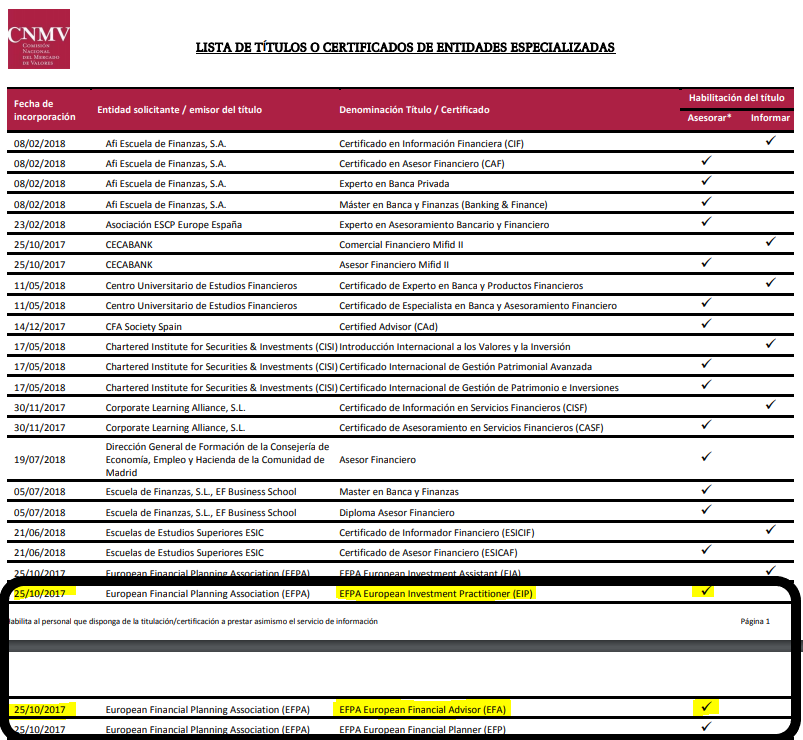
\includegraphics{./images/lista_titulos.png}

muchos de los candidatos/as están optando por certificarse como Asesor
Europeo (EFA) primero a través del examen EIP y, una vez que este se
encuentra aprobado, EFPA te ofrece la posibilidad de acceder al EFA
Completo a través de un examen ``parcial'' que sólo supone el 40\%
restante del contenido EFA Completo. Es como decir, que \textbf{el EFA
Completo se compone de,}

\begin{itemize}
\item
  \textbf{EIP: incluye el 60\% del contenido del EFA Completo}
\item
  \textbf{EFA Nivel II: incluye el 40\% restante del contenido del EFA
  Completo.}
\end{itemize}

\hypertarget{quuxe9-diferencias-hay-entre-eip-y-efa}{%
\section*{\texorpdfstring{\textbf{¿Qué diferencias hay entre EIP y
EFA?}}{¿Qué diferencias hay entre EIP y EFA?}}\label{quuxe9-diferencias-hay-entre-eip-y-efa}}
\addcontentsline{toc}{section}{\textbf{¿Qué diferencias hay entre EIP y
EFA?}}

\markright{\textbf{¿Qué diferencias hay entre EIP y EFA?}}

Como hemos dicho más arriba, una de las acreditaciones más demandadas
actualmente es la nueva certificación EIP, que de una forma resumida,
incluye el siguiente programa de contenidos:

\begin{longtable}[]{@{}clc@{}}
\toprule()
\endhead
Módulo 1 & Instrumentos y mercados financieros & 40,00\% \\
Módulo 2 & Fondos y sociedades de inversión mobiliaria & 10,00\% \\
Módulo 3 & Gestión de carteras & 12,50\% \\
Módulo 4 & Seguros & 7,50\% \\
Módulo 5 & Planes y fondos de pensiones & 5,00\% \\
Módulo 6 & Fiscalidad & 10,00\% \\
Módulo 7 & Cumplimiento normativo y regulador & 7,50\% \\
Módulo 8 & Asesoramiento y planificación financiera & 7,50\% \\
\bottomrule()
\end{longtable}

La siguiente certificación más demanda, y ya consolidada en el mercado,
es la certificación de asesor financiero europeo EFA. Este prestigio
examen incluye el siguiente programa de contenidos:

\begin{longtable}[]{@{}clc@{}}
\toprule()
\endhead
Módulo 1 & Instrumentos y mercados financieros & 25,00\% \\
Módulo 2 & Fondos y sociedades de inversión mobiliaria & 10,00\% \\
Módulo 3 & Gestión de carteras & 17,50\% \\
Módulo 4 & Seguros & 7,50\% \\
Módulo 5 & Pensiones y planificación de jubilación & 5,00\% \\
Módulo 6 & \textbf{Inversión Inmobiliaria} & 5,00\% \\
Módulo 7 & \textbf{Crédito y financiación} & 5,00\% \\
Módulo 8 & Fiscalidad & 10,00\% \\
Módulo 9 & Cumplimiento normativo y regulador & 7,50\% \\
Módulo 10 & Asesoramiento y planificación financiera & 7,50\% \\
\bottomrule()
\end{longtable}

Como se aprecia en los programas EFPA anteriores, el temario del examen
EFA incluye dos módulos más que el temario del examen EIP. Concretamente
los módulos de Inversión Inmobiliaria y, Crédito y financiación.
Asimismo, existen diferencias entre ambos exámenes en los contenidos de
cada uno de los módulos aunque estos tengan el mismo nombre.

Por lo tanto podemos optar por empezar esta formación de forma parcial,
es decir \textbf{podemos acreditarnos como EIP y más tarde como EFA
aprovechando lo común de los contenidos}. De forma que el examen EIP (o
de nivel I):

\begin{longtable}[]{@{}
  >{\centering\arraybackslash}p{(\columnwidth - 6\tabcolsep) * \real{0.2432}}
  >{\raggedright\arraybackslash}p{(\columnwidth - 6\tabcolsep) * \real{0.2703}}
  >{\centering\arraybackslash}p{(\columnwidth - 6\tabcolsep) * \real{0.2432}}
  >{\centering\arraybackslash}p{(\columnwidth - 6\tabcolsep) * \real{0.2432}}@{}}
\toprule()
\begin{minipage}[b]{\linewidth}\centering
\textbf{Módulo}
\end{minipage} & \begin{minipage}[b]{\linewidth}\raggedright
\textbf{Contenidos}
\end{minipage} & \begin{minipage}[b]{\linewidth}\centering
\textbf{Peso}
\end{minipage} & \begin{minipage}[b]{\linewidth}\centering
\textbf{Nº Preguntas}
\end{minipage} \\
\midrule()
\endhead
Módulo 1 & Instrumentos y mercados financieros & 40,00\% & 16 \\
Módulo 2 & Fondos y sociedades de inversión mobiliaria & 10,00\% & 4 \\
Módulo 3 & Gestión de carteras & 12,50\% & 5 \\
Módulo 4 & Seguros & 7,50\% & 3 \\
Módulo 5 & Planes y fondos de pensiones & 5,00\% & 2 \\
Módulo 6 & Fiscalidad & 10,00\% & 4 \\
Módulo 7 & Cumplimiento normativo y regulador & 7,50\% & 3 \\
Módulo 8 & Asesoramiento y planificación financiera & 7,50\% & 3 \\
\textbf{Total}: & & \textbf{100\%} & \textbf{40} \\
\bottomrule()
\end{longtable}

EFPA España ya ha previsto esto y es por ello que ofrece una solución en
la cual el aspirante se acredita primero como EIP y más tarde cabe la
posibilidad de hacer un ``curso puente2 -digamos- que le permitiría al
alumno examinarse de aquellos contenidos que son exclusivos de la
certificación EFPA. Este examen es conocido como examen de''nivel II'' y
es convocado por la Asociación 4 veces al año.

Además, la estructura de cada uno de estos exámenes es diferente como
vemos a continuación:

\hypertarget{estructura-examen-eip}{%
\section*{\texorpdfstring{\textbf{Estructura examen
EIP}}{Estructura examen EIP}}\label{estructura-examen-eip}}
\addcontentsline{toc}{section}{\textbf{Estructura examen EIP}}

\markright{\textbf{Estructura examen EIP}}

El examen EIP consta de 40 preguntas tipo test. Es requisito responder,
al menos, el 70\% de las preguntas del examen correctamente (28
preguntas), para superar satisfactoriamente la prueba. Las respuestas
incorrectas o en blanco no restan puntos. Duración del examen es de 1
hora y 30 minutos.

\hypertarget{estructura-examen-efa-nivel-ii}{%
\section*{\texorpdfstring{\textbf{Estructura examen EFA nivel
II}}{Estructura examen EFA nivel II}}\label{estructura-examen-efa-nivel-ii}}
\addcontentsline{toc}{section}{\textbf{Estructura examen EFA nivel II}}

\markright{\textbf{Estructura examen EFA nivel II}}

\hypertarget{constaruxe1-de-2-partes}{%
\subsection*{Constará de 2 partes:}\label{constaruxe1-de-2-partes}}
\addcontentsline{toc}{subsection}{Constará de 2 partes:}

\begin{enumerate}
\def\labelenumi{\arabic{enumi}.}
\item
  La primera, un examen tipo test de 40 preguntas. Para aprobar, el
  requisito será el haber respondido bien al menos al 70\% del examen
  (28 preguntas). Las respuestas incorrectas o en blanco no restan
  puntos. Duración de la primera prueba: 1 hora y 30 minutos.
\item
  La segunda parte, consistirá en la resolución de ejercicios prácticos
  sobre distintos aspectos contemplados en el temario EFA. Duración de
  la segunda prueba: 1 hora.
\end{enumerate}

Deben aprobarse ambas partes.

\hypertarget{estructura-examen-efa-completo}{%
\section*{\texorpdfstring{\textbf{Estructura examen EFA
completo}}{Estructura examen EFA completo}}\label{estructura-examen-efa-completo}}
\addcontentsline{toc}{section}{\textbf{Estructura examen EFA completo}}

\markright{\textbf{Estructura examen EFA completo}}

\hypertarget{constaruxe1-de-2-partes-1}{%
\subsection*{Constará de 2 partes:}\label{constaruxe1-de-2-partes-1}}
\addcontentsline{toc}{subsection}{Constará de 2 partes:}

\begin{enumerate}
\def\labelenumi{\arabic{enumi}.}
\item
  La primera, un examen tipo test de 50 preguntas. Para aprobar, el
  requisito será el haber respondido bien al menos al 70\% del examen
  (35 preguntas). Las respuestas incorrectas o en blanco no restan
  puntos. Duración de la primera prueba: 1 hora y 30 minutos.
\item
  La segunda parte, consistirá en la resolución de ejercicios prácticos
  sobre distintos aspectos contemplados en el temario EFA. Duración de
  la segunda prueba: 1 hora.
\end{enumerate}

Deben aprobarse ambas partes.

\hypertarget{necesito-alguxfan-requisito-para-acceder-a-las-acreditaciones-profesionales-de-efpa}{%
\section*{\texorpdfstring{\textbf{¿Necesito algún requisito para acceder
a las acreditaciones profesionales de
EFPA}}{¿Necesito algún requisito para acceder a las acreditaciones profesionales de EFPA}}\label{necesito-alguxfan-requisito-para-acceder-a-las-acreditaciones-profesionales-de-efpa}}
\addcontentsline{toc}{section}{\textbf{¿Necesito algún requisito para
acceder a las acreditaciones profesionales de EFPA}}

\markright{\textbf{¿Necesito algún requisito para acceder a las
acreditaciones profesionales de EFPA}}

EFPA exige unos requisitos mínimos y que estos van en función de qué
certificación queramos obtener. A continuación se presenta la
comparativa entre la certificación EIP y EFA:

\hypertarget{requisitos-examen-eip}{%
\subsection*{\texorpdfstring{\textbf{Requisitos examen
EIP}}{Requisitos examen EIP}}\label{requisitos-examen-eip}}
\addcontentsline{toc}{subsection}{\textbf{Requisitos examen EIP}}

Disponer de titulación completa de estudios secundarios.

Carecer de antecedentes penales por delitos dolosos, no haber sido
objeto de expulsión en colegio o asociación profesional y no haberle
impuesto sanción firme por infracción grave en la CNMV.

Acreditar 6 meses de experiencia en el sector financiero.

Realizar la inscripción al examen, a través de la Web de EFPA,
cumplimentando los datos requeridos, adjuntando CV, la última titulación
académica obtenida y realizar la transferencia de los derechos de examen
para finalizar el proceso (181,50 IVA incluido).

\hypertarget{requisitos-examen-efa}{%
\subsection*{\texorpdfstring{\textbf{Requisitos examen
EFA}}{Requisitos examen EFA}}\label{requisitos-examen-efa}}
\addcontentsline{toc}{subsection}{\textbf{Requisitos examen EFA}}

Disponer de titulación completa de estudios secundarios.

Se requiere 1 año de experiencia para poder obtener la certificación EFA
o bien, 6 meses, si el candidato ha realizado un curso de preparación en
un centro Acreditado. Una vez, el candidato ha obtenido el APTO, sino
dispone de la experiencia necesaria se le conserva el resultado durante
3 años, o hasta que demuestre haber obtenido la experiencia requerida y
así poder darse de alta en la asociación.

Carecer de antecedentes penales por delitos dolosos, no haber sido
objeto de expulsión en colegio o asociación profesional y no haberle
impuesto sanción firme por infracción grave en la CNMV.

Realizar la inscripción al examen, a través de la Web, cumplimentando
los datos requeridos, adjuntando CV, la última titulación académica
obtenida y realizar la transferencia de los derechos de examen para
finalizar el proceso (225 euros + 21\% IVA).

\part{EJERCICIOS RESUELTOS}

\hypertarget{muxf3dulo-1}{%
\chapter*{Módulo 1}\label{muxf3dulo-1}}
\addcontentsline{toc}{chapter}{Módulo 1}

\markboth{Módulo 1}{Módulo 1}

\hypertarget{comprender-los-factores-macroeconuxf3micos-que-afectan-a-los-rendimientos-de-la-inversiuxf3n}{%
\section*{Comprender los factores macroeconómicos que afectan a los
rendimientos de la
inversión}\label{comprender-los-factores-macroeconuxf3micos-que-afectan-a-los-rendimientos-de-la-inversiuxf3n}}
\addcontentsline{toc}{section}{Comprender los factores macroeconómicos
que afectan a los rendimientos de la inversión}

\markright{Comprender los factores macroeconómicos que afectan a los
rendimientos de la inversión}

\begin{enumerate}
\def\labelenumi{\arabic{enumi}.}
\tightlist
\item
  Si en un país, los tipos de interés están al 0.5\%, la inflación al
  4\% y el crecimiento del PIB en el -0.5\%. ¿Qué se espera que haga el
  país para aumentar su producción?
\end{enumerate}

\begin{enumerate}
\def\labelenumi{\alph{enumi})}
\item
  Disminuir tipos de interés.
\item
  Reducir la cantidad de dinero en circulación para que los individuos
  consuman más.
\item
  Devaluar la moneda para incrementar las exportaciones.
\item
  Ninguna de las anteriores.
\end{enumerate}

\begin{tcolorbox}[enhanced jigsaw, colback=white, colframe=quarto-callout-tip-color-frame, rightrule=.15mm, opacityback=0, toprule=.15mm, leftrule=.75mm, arc=.35mm, breakable, bottomrule=.15mm, left=2mm]
\begin{minipage}[t]{5.5mm}
\textcolor{quarto-callout-tip-color}{\faLightbulb}
\end{minipage}%
\begin{minipage}[t]{\textwidth - 5.5mm}

La respuesta \textbf{correcta es la c}.

A pesar de que la devaluación de la moneda puede ser generadora de
inflación, se puede interpretar que el problema más importante de la
economía es el crecimiento económico negativo, y por ello debe tomarse
alguna medida encaminada a fomentar el aumento del PIB, por ello una
devaluación, puede generar aspectos competitivos favorables, en la
medida que pueda fomentar el aumento de las exportaciones y la reducción
de las importaciones, lo que llevaría a aumentar el PIB.

El tipo de interés ya está en unos niveles muy bajos y por ello el
margen de actuación de la Política Monetaria es escaso o nulo.

Reducir la cantidad de dinero en circulación para que los individuos
consuman más, parece absurdo ya que la reducción de dinero produciría un
aumento de los tipos de interés, lo que en principio sería un factor
perjudicial para fomentar el crecimiento económico.

\end{minipage}%
\end{tcolorbox}

\begin{center}\rule{0.5\linewidth}{0.5pt}\end{center}

\begin{enumerate}
\def\labelenumi{\arabic{enumi}.}
\setcounter{enumi}{1}
\tightlist
\item
  Si una empresa española produce jamones en España y los exporta a
  Japón, a efectos del PIB que contribución se produce:
\end{enumerate}

\begin{enumerate}
\def\labelenumi{\alph{enumi})}
\item
  El PIB español aumenta
\item
  El PIB español se mantiene
\item
  El PIB japonés disminuye
\item
  a y c son correctas
\end{enumerate}

\begin{tcolorbox}[enhanced jigsaw, colback=white, colframe=quarto-callout-tip-color-frame, rightrule=.15mm, opacityback=0, toprule=.15mm, leftrule=.75mm, arc=.35mm, breakable, bottomrule=.15mm, left=2mm]
\begin{minipage}[t]{5.5mm}
\textcolor{quarto-callout-tip-color}{\faLightbulb}
\end{minipage}%
\begin{minipage}[t]{\textwidth - 5.5mm}

La respuesta \textbf{correcta es la d}.

Aumenta el PIB español porque los jamones se producen en España y se
exportan a otro país, por otra parte el PIB japonés disminuye porque la
empresa española exporta a Japón y para el PIB japonés se considera una
importación.

\end{minipage}%
\end{tcolorbox}

\begin{center}\rule{0.5\linewidth}{0.5pt}\end{center}

\begin{enumerate}
\def\labelenumi{\arabic{enumi}.}
\setcounter{enumi}{2}
\tightlist
\item
  ¿Cuál de las siguientes frases es sinónimo de un futura tendencia
  expansiva?
\end{enumerate}

\begin{enumerate}
\def\labelenumi{\alph{enumi})}
\item
  Paso de 55 a 45 en el ISM.
\item
  Paso de 95 a 90 en el IFO.
\item
  Paso de 45 a 55 en el IFO.
\item
  Paso de 45 a 55 en el ISM.
\end{enumerate}

\begin{tcolorbox}[enhanced jigsaw, colback=white, colframe=quarto-callout-tip-color-frame, rightrule=.15mm, opacityback=0, toprule=.15mm, leftrule=.75mm, arc=.35mm, breakable, bottomrule=.15mm, left=2mm]
\begin{minipage}[t]{5.5mm}
\textcolor{quarto-callout-tip-color}{\faLightbulb}
\end{minipage}%
\begin{minipage}[t]{\textwidth - 5.5mm}

La respuesta \textbf{correcta es la d}.

El Indicador ISM es un indicador avanzado de producción americano. Se
elabora mensualmente una encuesta a los jefes de compra de 250 empresas
en la cual se les pide que respondan si la actividad será igual, mayor o
inferior a la del mes anterior. A partir de los resultados se
interpretará si va a haber una \textbf{tendencia expansiva} (en el caso
de que la actividad sea mayor) o recesiva (en el caso de que la
actividad sea menor) en la economía.

El Indicador IFO es un indicador avanzado de producción alemán. Se
elabora una encuesta a 10.000 empresas alemanas acerca de las
actividades presentes de cada empresa y de las actividades previstas en
los próximos seis meses. Si la tendencia es alcista, tiende a
interpretarse como una \textbf{recuperación de la economía}, y
viceversa. Aunque es un indicador alemán, su interpretación suele
extrapolarse al resto de la economía europea. Este indicador se elabora
de forma mensual.

\end{minipage}%
\end{tcolorbox}

\begin{center}\rule{0.5\linewidth}{0.5pt}\end{center}

\begin{enumerate}
\def\labelenumi{\arabic{enumi}.}
\setcounter{enumi}{3}
\tightlist
\item
  Si el incremento del PIB americano ha pasado de ser el 2\% al 8\%.
  ¿Por qué ha podido pasar?
\end{enumerate}

\begin{enumerate}
\def\labelenumi{\alph{enumi})}
\item
  Porque en Estados Unidos siempre aumenta el PIB, ya que su economía es
  la principal economía mundial y nunca atraviesa fases de recesión.
\item
  Porque han aumentado mucho las importaciones.
\item
  Porque han aumentado mucho las exportaciones.
\item
  Todas las respuestas anteriores son correctas.
\end{enumerate}

\begin{tcolorbox}[enhanced jigsaw, colback=white, colframe=quarto-callout-tip-color-frame, rightrule=.15mm, opacityback=0, toprule=.15mm, leftrule=.75mm, arc=.35mm, breakable, bottomrule=.15mm, left=2mm]
\begin{minipage}[t]{5.5mm}
\textcolor{quarto-callout-tip-color}{\faLightbulb}
\end{minipage}%
\begin{minipage}[t]{\textwidth - 5.5mm}

La respuesta \textbf{correcta es la c}.

Porque han aumentado mucho las exportaciones, ya que las importaciones
restan valor al PIB, por lo que un aumento de éstas hará disminuir el
PIB, en cambio las exportaciones suman al PIB por lo que su aumento hará
incrementar el PIB.

\end{minipage}%
\end{tcolorbox}

\begin{center}\rule{0.5\linewidth}{0.5pt}\end{center}

\begin{enumerate}
\def\labelenumi{\arabic{enumi}.}
\setcounter{enumi}{4}
\tightlist
\item
  ¿Qué soluciones tiene Australia para reducir la tasa de paro?
\end{enumerate}

\begin{enumerate}
\def\labelenumi{\alph{enumi})}
\item
  Que el Banco Central reduzca tipos de interés
\item
  Que se deprecie el dólar australiano
\item
  Aplicar incentivos para la contratación de gente joven y mayor de 55
  años
\item
  Todas las acciones anteriores son correctas
\end{enumerate}

\begin{tcolorbox}[enhanced jigsaw, colback=white, colframe=quarto-callout-tip-color-frame, rightrule=.15mm, opacityback=0, toprule=.15mm, leftrule=.75mm, arc=.35mm, breakable, bottomrule=.15mm, left=2mm]
\begin{minipage}[t]{5.5mm}
\textcolor{quarto-callout-tip-color}{\faLightbulb}
\end{minipage}%
\begin{minipage}[t]{\textwidth - 5.5mm}

La respuesta \textbf{correcta es la d}.

Si el Banco Central disminuye tipos de interés, a las empresas les
costará menos endeudarse, por lo que incrementarán sus inversiones. Este
aumento de las inversiones hará que se necesite a más gente para
llevarlas a cabo.

Si se deprecia el dólar australiano las empresas australianas producirán
más, ya que parte de su producción la venderán en el extranjero, por lo
que necesitarán a más gente para trabajar. Si aplican incentivos para la
contratación de personas, las empresas adaptarán estas ventajas
contratando a gente.

\end{minipage}%
\end{tcolorbox}

\begin{center}\rule{0.5\linewidth}{0.5pt}\end{center}

\begin{enumerate}
\def\labelenumi{\arabic{enumi}.}
\setcounter{enumi}{5}
\tightlist
\item
  Cual de las siguientes respuestas es correcta en el supuesto que el
  déficit público de Rusia aumente.
\end{enumerate}

\begin{enumerate}
\def\labelenumi{\alph{enumi})}
\item
  Aumenta el déficit público debido a que han disminuido los ingresos
  derivados de los impuestos
\item
  Aumenta debido a un incremento del gasto público mayor al esperado
\item
  Se espera que los bonos emitidos por el gobierno tengan un tipo de
  interés mayor
\item
  Todas las respuestas anteriores son correctas
\end{enumerate}

\begin{tcolorbox}[enhanced jigsaw, colback=white, colframe=quarto-callout-tip-color-frame, rightrule=.15mm, opacityback=0, toprule=.15mm, leftrule=.75mm, arc=.35mm, breakable, bottomrule=.15mm, left=2mm]
\begin{minipage}[t]{5.5mm}
\textcolor{quarto-callout-tip-color}{\faLightbulb}
\end{minipage}%
\begin{minipage}[t]{\textwidth - 5.5mm}

La respuesta \textbf{correcta es la d}.

El déficit público se genera cuando los gastos del Estado son mayores a
sus ingresos. Por lo que una disminución de los ingresos, un incremento
del gasto o ambas cosas a la vez harán aumentar el déficit público. Si
aumenta el déficit público, Rusia deberá emitir deuda para obtener
ingresos adicionales, para incentivar a que los inversores compren su
deuda, deberá aumentar el tipo de interés.

\end{minipage}%
\end{tcolorbox}

\begin{center}\rule{0.5\linewidth}{0.5pt}\end{center}

\begin{enumerate}
\def\labelenumi{\arabic{enumi}.}
\setcounter{enumi}{6}
\tightlist
\item
  ¿Cuál de las siguientes fases corresponden a un período de crecimiento
  del PIB?:
\end{enumerate}

\begin{enumerate}
\def\labelenumi{\alph{enumi})}
\item
  Expansión
\item
  Recesión
\item
  Estancamiento
\item
  Contracción
\end{enumerate}

\begin{tcolorbox}[enhanced jigsaw, colback=white, colframe=quarto-callout-tip-color-frame, rightrule=.15mm, opacityback=0, toprule=.15mm, leftrule=.75mm, arc=.35mm, breakable, bottomrule=.15mm, left=2mm]
\begin{minipage}[t]{5.5mm}
\textcolor{quarto-callout-tip-color}{\faLightbulb}
\end{minipage}%
\begin{minipage}[t]{\textwidth - 5.5mm}

La respuesta \textbf{correcta es la a}.

La única fase que corresponde a un período de crecimiento es la
``Expansión''. El resto de fases descritas debieran coincidir con
reducción del crecimiento del PIB o estabilidad del mismo.

\end{minipage}%
\end{tcolorbox}

\begin{center}\rule{0.5\linewidth}{0.5pt}\end{center}

\begin{enumerate}
\def\labelenumi{\arabic{enumi}.}
\setcounter{enumi}{7}
\tightlist
\item
  ¿Cuál es el agregado que se suele utilizar para medir el crecimiento
  de una economía?:
\end{enumerate}

\begin{enumerate}
\def\labelenumi{\alph{enumi})}
\item
  FBCF
\item
  PIB
\item
  IPC
\item
  PER
\end{enumerate}

\begin{tcolorbox}[enhanced jigsaw, colback=white, colframe=quarto-callout-tip-color-frame, rightrule=.15mm, opacityback=0, toprule=.15mm, leftrule=.75mm, arc=.35mm, breakable, bottomrule=.15mm, left=2mm]
\begin{minipage}[t]{5.5mm}
\textcolor{quarto-callout-tip-color}{\faLightbulb}
\end{minipage}%
\begin{minipage}[t]{\textwidth - 5.5mm}

La respuesta \textbf{correcta es la b}.

El agregado universal más utilizado es el PIB o Producto Interior Bruto.
El PIB desde el punto de vista de la demanda queda integrado por la suma
de consumo privado nacional, consumo público, formación bruta del
capital fijo o inversión, variación de las existencias (inventarios) y
exportación de bienes y servicios, restando de dichas cifras las
importaciones.

La Formación Bruta del Capital Fijo es una componente del PIB, mientras
que el IPC o Índice de Precios al Consumo hace referencia a la inflación
o crecimiento general de los precios de la economía, pero se utiliza
como referencia de crecimiento de una economía.

El PER (Price earning ratio) es un ratio bursátil.

\end{minipage}%
\end{tcolorbox}

\begin{center}\rule{0.5\linewidth}{0.5pt}\end{center}

\begin{enumerate}
\def\labelenumi{\arabic{enumi}.}
\setcounter{enumi}{8}
\tightlist
\item
  ¿Qué se suele entender comúnmente por recesión?:
\end{enumerate}

\begin{enumerate}
\def\labelenumi{\alph{enumi})}
\item
  Cualquier reducción que se produzca en el PIB de un período respecto
  al período anterior
\item
  Tres meses consecutivos con tasas de variación del PIB negativas
\item
  Tres trimestres consecutivos con tasas de variación del PIB negativas
\item
  Ninguna de las anteriores
\end{enumerate}

\begin{tcolorbox}[enhanced jigsaw, colback=white, colframe=quarto-callout-tip-color-frame, rightrule=.15mm, opacityback=0, toprule=.15mm, leftrule=.75mm, arc=.35mm, breakable, bottomrule=.15mm, left=2mm]
\begin{minipage}[t]{5.5mm}
\textcolor{quarto-callout-tip-color}{\faLightbulb}
\end{minipage}%
\begin{minipage}[t]{\textwidth - 5.5mm}

La respuesta \textbf{correcta es la d}.

A pesar de que pueden existir algunas opiniones discrepantes, ya que no
se trata de un criterio universal o matemáticamente indiscutible, es
frecuente considerar que recesión son dos trimestres consecutivos con
tasas de variación del PIB negativas.

\end{minipage}%
\end{tcolorbox}

\begin{center}\rule{0.5\linewidth}{0.5pt}\end{center}

\begin{enumerate}
\def\labelenumi{\arabic{enumi}.}
\setcounter{enumi}{9}
\tightlist
\item
  ¿Qué tipo de indicador es el de ventas minoristas?
\end{enumerate}

\begin{enumerate}
\def\labelenumi{\alph{enumi})}
\item
  Indicador de demanda
\item
  Indicador de oferta
\item
  Indicador de producción
\item
  Indicador de precios
\end{enumerate}

\begin{tcolorbox}[enhanced jigsaw, colback=white, colframe=quarto-callout-tip-color-frame, rightrule=.15mm, opacityback=0, toprule=.15mm, leftrule=.75mm, arc=.35mm, breakable, bottomrule=.15mm, left=2mm]
\begin{minipage}[t]{5.5mm}
\textcolor{quarto-callout-tip-color}{\faLightbulb}
\end{minipage}%
\begin{minipage}[t]{\textwidth - 5.5mm}

La respuesta \textbf{correcta es la a}.

Si se tuviera que definir indicador de demanda, se podría decir que es
aquel que refleja diversos aspectos de la evolución del consumo privado
y el comportamiento de los consumidores. Por ello el indicador ``Ventas
al por menor'' se ubica en el grupo de indicadores de demanda.

No es indicador de sentimiento porque no se basa en encuestas periódicas
sobre las expectativas de los agentes económicos, tampoco es indicador
de oferta pues no se basa en datos económicos que reflejen diversos
aspectos de la evolución de la producción, y tampoco es un indicador de
la evolución de los precios.

\end{minipage}%
\end{tcolorbox}

\begin{center}\rule{0.5\linewidth}{0.5pt}\end{center}

\begin{enumerate}
\def\labelenumi{\arabic{enumi}.}
\setcounter{enumi}{10}
\tightlist
\item
  En una fase de ciclo en situación expansiva y con alza importante de
  precios, el director y/o ejecutor de la Política Monetaria podría
  tomar decisiones encaminadas a:
\end{enumerate}

\begin{enumerate}
\def\labelenumi{\alph{enumi})}
\item
  Subir los tipos de interés a corto plazo.
\item
  Bajar los tipos de interés a corto plazo.
\item
  Bajar los tipos de interés a largo plazo.
\item
  Ninguno de los anteriores.
\end{enumerate}

\begin{tcolorbox}[enhanced jigsaw, colback=white, colframe=quarto-callout-tip-color-frame, rightrule=.15mm, opacityback=0, toprule=.15mm, leftrule=.75mm, arc=.35mm, breakable, bottomrule=.15mm, left=2mm]
\begin{minipage}[t]{5.5mm}
\textcolor{quarto-callout-tip-color}{\faLightbulb}
\end{minipage}%
\begin{minipage}[t]{\textwidth - 5.5mm}

La respuesta \textbf{correcta es la a}.

Al producirse una situación que conlleva ``sobrecalentamiento'' de la
economía, una decisión habitual de los Bancos Centrales es la subida de
tipos de interés, para que con ello se fomente el ahorro, la inversión
empresarial y se modere el consumo, lo que podría llevar a una menor
presión sobre el crecimiento de los precios, a pesar de que también
puede frenar el nivel de crecimiento del PIB.

Bajar los tipos de interés por parte del Banco Central, podría ser una
decisión coherente en un contexto de bajo crecimiento positivo,
crecimiento nulo o negativo del PIB, y con ello se propiciaría un
desincentivo para el ahorro, una mayor inversión empresarial y un mayor
consumo y mayor crecimiento del PIB.

En lo que respecta a la influencia de los Bancos Centrales sobre los
tipos de interés a largo plazo, debe decirse que la misma es escasa al
menos de forma directa a través de las intervenciones en los mercados,
si que pueden ser más influyentes las expectativas que puedan generar
los responsables de las políticas monetarias.

\end{minipage}%
\end{tcolorbox}

\begin{center}\rule{0.5\linewidth}{0.5pt}\end{center}

\begin{enumerate}
\def\labelenumi{\arabic{enumi}.}
\setcounter{enumi}{11}
\tightlist
\item
  Un factor de cierta importancia para frenar la inflación es:
\end{enumerate}

\begin{enumerate}
\def\labelenumi{\alph{enumi})}
\item
  Aumento del déficit público
\item
  Reducción del déficit público
\item
  Políticas monetarias claramente expansivas
\item
  Aumento de los impuestos indirectos
\end{enumerate}

\begin{tcolorbox}[enhanced jigsaw, colback=white, colframe=quarto-callout-tip-color-frame, rightrule=.15mm, opacityback=0, toprule=.15mm, leftrule=.75mm, arc=.35mm, breakable, bottomrule=.15mm, left=2mm]
\begin{minipage}[t]{5.5mm}
\textcolor{quarto-callout-tip-color}{\faLightbulb}
\end{minipage}%
\begin{minipage}[t]{\textwidth - 5.5mm}

La respuesta \textbf{correcta es la b}.

De todas las respuestas la única posible es la que hace referencia a la
reducción del déficit público, ya que se interpreta que el mismo puede
venir por la vía de la reducción del gasto público, lo que supone una
menor aportación al crecimiento del PIB, lo que puede generar no sólo
menor consumo público, sino también menor crecimiento económico privado,
menor formación bruta del capital y en definitiva todo ello son factores
atenuantes del crecimiento económico y también en consecuencia de la
presión inflacionista.

El aumento del déficit público y las políticas monetarias expansivas
(reducción de los tipos de interés y aumento de la cantidad de dinero en
circulación) son generadores de posible crecimiento económico, en
ocasiones más a corto que a largo plazo, pero son generadoras de aumento
general de los precios.

Los impuestos indirectos en la medida que se repercuten en el precio
final de los bienes y servicios, conllevan también un aumento de la
inflación.

\end{minipage}%
\end{tcolorbox}

\begin{center}\rule{0.5\linewidth}{0.5pt}\end{center}

\begin{enumerate}
\def\labelenumi{\arabic{enumi}.}
\setcounter{enumi}{12}
\tightlist
\item
  ¿Qué tipo de indicador es el IFO alemán?:
\end{enumerate}

\begin{enumerate}
\def\labelenumi{\alph{enumi})}
\item
  Indicador de demanda
\item
  Indicador de oferta
\item
  Indicador de precios
\item
  Indicador de sentimiento
\end{enumerate}

\begin{tcolorbox}[enhanced jigsaw, colback=white, colframe=quarto-callout-tip-color-frame, rightrule=.15mm, opacityback=0, toprule=.15mm, leftrule=.75mm, arc=.35mm, breakable, bottomrule=.15mm, left=2mm]
\begin{minipage}[t]{5.5mm}
\textcolor{quarto-callout-tip-color}{\faLightbulb}
\end{minipage}%
\begin{minipage}[t]{\textwidth - 5.5mm}

La respuesta \textbf{correcta es la d}.

El IFO es un índice de clima empresarial, que se publica mensualmente
por parte del Instituto de Investigación Económica de Alemania y que
informa sobre el sentimiento de diversos sectores productivos y sus
expectativas. Asimismo, el IFO se puede considerar un índice adelantando
de actividad económica.

\end{minipage}%
\end{tcolorbox}

\begin{center}\rule{0.5\linewidth}{0.5pt}\end{center}

\begin{enumerate}
\def\labelenumi{\arabic{enumi}.}
\setcounter{enumi}{13}
\tightlist
\item
  ¿Qué tipo de indicador es el de ``Utilización de la capacidad
  productiva Capacity utilization?:
\end{enumerate}

\begin{enumerate}
\def\labelenumi{\alph{enumi})}
\item
  Indicador de demanda
\item
  Indicador de oferta
\item
  Indicador de precios
\item
  Indicador de sentimiento
\end{enumerate}

\begin{tcolorbox}[enhanced jigsaw, colback=white, colframe=quarto-callout-tip-color-frame, rightrule=.15mm, opacityback=0, toprule=.15mm, leftrule=.75mm, arc=.35mm, breakable, bottomrule=.15mm, left=2mm]
\begin{minipage}[t]{5.5mm}
\textcolor{quarto-callout-tip-color}{\faLightbulb}
\end{minipage}%
\begin{minipage}[t]{\textwidth - 5.5mm}

La respuesta \textbf{correcta es la b}.

Se trata de un indicador de oferta, pues está vinculado, como su propio
nombre indica, con aspectos vinculados a la evolución de la producción.

No es un índice de precios, no es de sentimiento pues se basa en datos
objetivos y no es indicador de demanda, ya que no da información sobre
el consumo privado o el comportamiento de los consumidores.

\end{minipage}%
\end{tcolorbox}

\begin{center}\rule{0.5\linewidth}{0.5pt}\end{center}

\begin{enumerate}
\def\labelenumi{\arabic{enumi}.}
\setcounter{enumi}{14}
\tightlist
\item
  De las siguientes situaciones, ¿cuál parece más lógica que suceda en
  plena etapa de recesión intensa?:
\end{enumerate}

\begin{enumerate}
\def\labelenumi{\alph{enumi})}
\item
  Paro al alza
\item
  Sentimiento económico al alza
\item
  Tipos de interés al alza
\item
  Bolsa al alza
\end{enumerate}

\begin{tcolorbox}[enhanced jigsaw, colback=white, colframe=quarto-callout-tip-color-frame, rightrule=.15mm, opacityback=0, toprule=.15mm, leftrule=.75mm, arc=.35mm, breakable, bottomrule=.15mm, left=2mm]
\begin{minipage}[t]{5.5mm}
\textcolor{quarto-callout-tip-color}{\faLightbulb}
\end{minipage}%
\begin{minipage}[t]{\textwidth - 5.5mm}

La respuesta \textbf{correcta es la a}.

Lo habitual es que con un PIB en fase de recesión se genere desempleo,
es decir incremento de las tasas de paro.

El resto de cuestiones parecen contradictorias con una fase de recesión
intensa, que normalmente debiera conllevar un sentimiento económico a la
baja o por los menos en niveles muy bajos.

No parece coherente subir los tipos de interés en fases de recesión
intenso, sino todo lo contrario, y lo habitual es que la Bolsa se
encuentre en fase bajista, a pesar de que la evolución de los mercados
bursátiles puede presentar ciertos desfases temporales respecto a la
evolución de la economía, debido a que con frecuencia se indica que los
precios de las acciones suelen descontar expectativas de futuras
situaciones económicas, potencialmente diferentes de la realidad actual.

\end{minipage}%
\end{tcolorbox}

\begin{center}\rule{0.5\linewidth}{0.5pt}\end{center}

\begin{enumerate}
\def\labelenumi{\arabic{enumi}.}
\setcounter{enumi}{15}
\tightlist
\item
  De las siguientes situaciones ¿cuál parece más lógica que suceda en
  plena etapa de expansión intensa?
\end{enumerate}

\begin{enumerate}
\def\labelenumi{\alph{enumi})}
\item
  Demanda a la baja
\item
  Paro a la baja
\item
  PIB a la baja
\item
  Bolsa a la baja
\end{enumerate}

\begin{tcolorbox}[enhanced jigsaw, colback=white, colframe=quarto-callout-tip-color-frame, rightrule=.15mm, opacityback=0, toprule=.15mm, leftrule=.75mm, arc=.35mm, breakable, bottomrule=.15mm, left=2mm]
\begin{minipage}[t]{5.5mm}
\textcolor{quarto-callout-tip-color}{\faLightbulb}
\end{minipage}%
\begin{minipage}[t]{\textwidth - 5.5mm}

La respuesta \textbf{correcta es la b}.

Lo habitual es que con un PIB en fase de expansión intensa, ello genere
reducción del desempleo, es decir caída de las tasas de paro y aumento
de las tasas de empleo.

El resto de cuestiones parece contradictorias con una fase de expansión
intensa, ya que si el crecimiento económico es intenso el PIB estará
aumentando, el nivel de demanda no debiera ir a la baja, sino todo lo
contrario y en lo que respecta a la Bolsa, lo habitual es que se
encuentre en fase alcista, a pesar de que la evolución de los mercados
bursátiles puede presentar ciertos desfases temporales respecto a la
evolución de la economía, debido a que con frecuencia se indica que los
precios de las acciones suelen descontar expectativas de futuras
situaciones económicas, potencialmente diferentes de la realidad actual.

\end{minipage}%
\end{tcolorbox}

\begin{center}\rule{0.5\linewidth}{0.5pt}\end{center}

\begin{enumerate}
\def\labelenumi{\arabic{enumi}.}
\setcounter{enumi}{16}
\tightlist
\item
  Si el euro se deprecia, se espera que:
\end{enumerate}

\begin{enumerate}
\def\labelenumi{\alph{enumi})}
\item
  El PIB europeo aumente
\item
  El PIB europeo disminuya
\item
  Que disminuya el turismo en Europa
\item
  Que el PIB de los países con los que mantiene relaciones comerciales
  aumente
\end{enumerate}

\begin{tcolorbox}[enhanced jigsaw, colback=white, colframe=quarto-callout-tip-color-frame, rightrule=.15mm, opacityback=0, toprule=.15mm, leftrule=.75mm, arc=.35mm, breakable, bottomrule=.15mm, left=2mm]
\begin{minipage}[t]{5.5mm}
\textcolor{quarto-callout-tip-color}{\faLightbulb}
\end{minipage}%
\begin{minipage}[t]{\textwidth - 5.5mm}

La respuesta \textbf{correcta es la a}.

La depreciación del euro, o si fuera la situación más drástica una
devaluación, debiera estar propiciada para aumentar el PIB medio de los
países que integran dicha zona económica y monetaria.

De hecho con la depreciación del euro, se podría estar buscando una
ventaja competitiva que se pondría de manifiesto inicialmente a través
del sector exterior, ya que las exportaciones serían más competitivas y
debieran de aumentar, mientras que las importaciones se encarecerían y
debieran disminuir, por todo ello el PIB debiera aumentar.

Todo ello, en un contexto de explicación simplificada, y sin tener en
cuenta otros muchos posibles efectos colaterales a corto, medio y largo
plazo.

\end{minipage}%
\end{tcolorbox}

\begin{center}\rule{0.5\linewidth}{0.5pt}\end{center}

\begin{enumerate}
\def\labelenumi{\arabic{enumi}.}
\setcounter{enumi}{17}
\tightlist
\item
  Ante una situación de recesión, el BCE puede:
\end{enumerate}

\begin{enumerate}
\def\labelenumi{\alph{enumi})}
\item
  Aumentar los tipos de interés para favorecer la inversión
\item
  Disminuir los tipos de interés para favorecer la inversión
\item
  Esperar a que mejore la economía porque hasta entonces él no puede
  intervenir
\item
  Comprar acciones en Bolsa para subir el valor de éstas
\end{enumerate}

\begin{tcolorbox}[enhanced jigsaw, colback=white, colframe=quarto-callout-tip-color-frame, rightrule=.15mm, opacityback=0, toprule=.15mm, leftrule=.75mm, arc=.35mm, breakable, bottomrule=.15mm, left=2mm]
\begin{minipage}[t]{5.5mm}
\textcolor{quarto-callout-tip-color}{\faLightbulb}
\end{minipage}%
\begin{minipage}[t]{\textwidth - 5.5mm}

La respuesta \textbf{correcta es la b}.

Una actuación académicamente poco cuestionable es que el Banco Central
Europeo acuda a la variable instrumental de los tipos de interés de
corto plazo para fomentar el crecimiento económico, por medio de una
reducción de los citados tipos de interés que debieran desincentivar el
ahorro y fomentar la inversión empresarial y el consumo, lo que podría
coadyuvar, con estas medidas y quizá con otras complementarias, a frenar
la recesión o entrar en un nuevo ciclo económico expansivo.

El Banco Central Europeo puede intervenir en los mercados monetarios y
de cambios cuando lo considere oportuno, y si estima que no es
conveniente intervenir pues no lo hace.

Por lo que respecta a la compra de acciones en Bolsa, se considera que
entre las funciones de un Banco Central no está la intervención en
mercados bursátiles, ya que el precio de las acciones debe fluctuar
según las condiciones de oferta y demanda de dichos mercados sin
injerencias oficiales.

\end{minipage}%
\end{tcolorbox}

\begin{center}\rule{0.5\linewidth}{0.5pt}\end{center}

\begin{enumerate}
\def\labelenumi{\arabic{enumi}.}
\setcounter{enumi}{18}
\tightlist
\item
  Si el nivel de inflación es elevado se espera:
\end{enumerate}

\begin{enumerate}
\def\labelenumi{\alph{enumi})}
\item
  Un aumento del tipo de interés
\item
  Una disminución de la inversión de las empresas
\item
  Una bajada del poder adquisitivo de los consumidores
\item
  Todas las respuestas anteriores son correctas
\end{enumerate}

\begin{tcolorbox}[enhanced jigsaw, colback=white, colframe=quarto-callout-tip-color-frame, rightrule=.15mm, opacityback=0, toprule=.15mm, leftrule=.75mm, arc=.35mm, breakable, bottomrule=.15mm, left=2mm]
\begin{minipage}[t]{5.5mm}
\textcolor{quarto-callout-tip-color}{\faLightbulb}
\end{minipage}%
\begin{minipage}[t]{\textwidth - 5.5mm}

La respuesta \textbf{correcta es la d}.

Debe responderse que todas las respuestas son correctas, ya que tanto el
aumento del tipo de interés, como la disminución empresarial y la bajada
de poder adquisitivo de los inversores son consecuencias lógicas y
coherentes con un nivel de inflación elevado.

\end{minipage}%
\end{tcolorbox}

\begin{center}\rule{0.5\linewidth}{0.5pt}\end{center}

\begin{enumerate}
\def\labelenumi{\arabic{enumi}.}
\setcounter{enumi}{19}
\tightlist
\item
  Si el BCE aumenta el tipo de interés, se espera:
\end{enumerate}

\begin{enumerate}
\def\labelenumi{\alph{enumi})}
\item
  Un aumento del valor de las acciones de las empresas europeas debido a
  la entrada de capitales provenientes de Estados Unidos
\item
  Una disminución del valor de las acciones de empresas europeas que
  cotizan en Estados Unidos.
\item
  Una disminución del valor de las acciones de empresas americanas
  debido al trasvase de fondos desde Europa a Estados Unidos
\item
  Todas las anteriores son correctas
\end{enumerate}

\begin{tcolorbox}[enhanced jigsaw, colback=white, colframe=quarto-callout-tip-color-frame, rightrule=.15mm, opacityback=0, toprule=.15mm, leftrule=.75mm, arc=.35mm, breakable, bottomrule=.15mm, left=2mm]
\begin{minipage}[t]{5.5mm}
\textcolor{quarto-callout-tip-color}{\faLightbulb}
\end{minipage}%
\begin{minipage}[t]{\textwidth - 5.5mm}

La respuesta \textbf{correcta es la b}.

\(\uparrow\) tipos de interés en Europa:

\begin{enumerate}
\def\labelenumi{\alph{enumi})}
\item
  \(\uparrow\) coste de la deuda \(\Rightarrow\) \(\downarrow\)
  inversiones \(\Rightarrow\) \(\downarrow\) beneficios
\item
  Nueva emisión de deuda pública con tipo de interés MAYOR
  \(\Rightarrow\) trasvase de fondos del mercado de renta variable al de
  renta fija \(\Rightarrow\) \(\uparrow\) demanada de valores de deuda
  \(\Rightarrow\) \(\downarrow\) valor de las acciones.
\end{enumerate}

\end{minipage}%
\end{tcolorbox}

\begin{center}\rule{0.5\linewidth}{0.5pt}\end{center}

\begin{enumerate}
\def\labelenumi{\arabic{enumi}.}
\setcounter{enumi}{20}
\tightlist
\item
  La reserva federal de Estados Unidos decide disminuir los tipos de
  interés. ¿Por qué crees que ha podido tomar esta decisión?
\end{enumerate}

\begin{enumerate}
\def\labelenumi{\alph{enumi})}
\item
  Para reducir la tasa de desempleo
\item
  Para incentivar el consumo del país
\item
  Para disminuir el coste de la deuda de las empresas
\item
  Todas las respuestas anteriores son correctas
\end{enumerate}

\begin{tcolorbox}[enhanced jigsaw, colback=white, colframe=quarto-callout-tip-color-frame, rightrule=.15mm, opacityback=0, toprule=.15mm, leftrule=.75mm, arc=.35mm, breakable, bottomrule=.15mm, left=2mm]
\begin{minipage}[t]{5.5mm}
\textcolor{quarto-callout-tip-color}{\faLightbulb}
\end{minipage}%
\begin{minipage}[t]{\textwidth - 5.5mm}

La respuesta \textbf{correcta es la d}.

Las tres respuestas son correctas, y todas ellas con mayor o menor
incidencia son factores que pueden producirse gracias a la reducción de
los tipos de interés de la Reserva Federal, que con su actuación
pretende generar un incremento del PIB, a pesar de que ello pueda ser un
factor que en mayor o menor medida genere inflación.

Los Bancos Centrales según la situación coyuntural, anteponen
crecimiento económico a inflación o viceversa, si bien es cierto que la
actuación de la Reserva Federal se plantea de forma más agresiva que la
del Banco Central Europeo. En la corta experiencia del Banco Central
Europeo, parece haberse dado mayor importancia al control de los
precios, mientras que la Reserva Federal no perdiendo la referencia del
crecimiento de los precios, parece anteponer habitualmente el
crecimiento económico como objetivo prioritario.

\end{minipage}%
\end{tcolorbox}

\begin{center}\rule{0.5\linewidth}{0.5pt}\end{center}

\begin{enumerate}
\def\labelenumi{\arabic{enumi}.}
\setcounter{enumi}{21}
\tightlist
\item
  Si el indicador ISM (NAPM) se sitúa por encima de 50 significa:
\end{enumerate}

\begin{enumerate}
\def\labelenumi{\alph{enumi})}
\item
  Que la confianza de los productores americanos ha aumentado
\item
  Que la confianza de los productores alemanes ha aumentado
\item
  Que la confianza de los productores americanos ha disminuido
\item
  Que la confianza de los consumidores americanos ha disminuido
\end{enumerate}

\begin{tcolorbox}[enhanced jigsaw, colback=white, colframe=quarto-callout-tip-color-frame, rightrule=.15mm, opacityback=0, toprule=.15mm, leftrule=.75mm, arc=.35mm, breakable, bottomrule=.15mm, left=2mm]
\begin{minipage}[t]{5.5mm}
\textcolor{quarto-callout-tip-color}{\faLightbulb}
\end{minipage}%
\begin{minipage}[t]{\textwidth - 5.5mm}

La respuesta \textbf{correcta es la a}.

El ISM (NAPM) es un indicador adelantado de actividad y sentimiento, es
un indicador manufacturero y se elabora por parte de la Nacional
Association of Purchasing Managers sobre las expectativas de la
actividad industrial, incorporando información sobre nuevos pedidos,
empleo, producción, inventarios, plazos de entrega, etc.

Se considera que si el NPAM está por encima de 50 la economía USA está
en expansión y la confianza de los productores americanos ha aumentado.

\end{minipage}%
\end{tcolorbox}

\begin{center}\rule{0.5\linewidth}{0.5pt}\end{center}

\begin{enumerate}
\def\labelenumi{\arabic{enumi}.}
\setcounter{enumi}{22}
\tightlist
\item
  Indicar cuál de las siguientes frases acerca de la inflación es
  correcta:
\end{enumerate}

\begin{enumerate}
\def\labelenumi{\alph{enumi})}
\item
  La inflación es un indicador retardado, aunque ayuda a definir la
  política monetaria de los bancos centrales
\item
  Una inflación positiva y controlada permite que los principales
  índices bursátiles aumenten de valor
\item
  La deflación implica que el consumo se reduzca
\item
  Todas las respuestas anteriores son correctas
\end{enumerate}

\begin{tcolorbox}[enhanced jigsaw, colback=white, colframe=quarto-callout-tip-color-frame, rightrule=.15mm, opacityback=0, toprule=.15mm, leftrule=.75mm, arc=.35mm, breakable, bottomrule=.15mm, left=2mm]
\begin{minipage}[t]{5.5mm}
\textcolor{quarto-callout-tip-color}{\faLightbulb}
\end{minipage}%
\begin{minipage}[t]{\textwidth - 5.5mm}

La respuesta \textbf{correcta es la d}.

Todas las respuestas anteriores son correctas y por debe remarcarse D).
Es cierto que la inflación es un indicador retardado, ya que se conoce
con varias semanas de retraso respecto a que se ha producido la misma, y
por ello retrasa la toma de decisiones por parte de las autoridades
monetarias. Es por ello, que algunas autoridades monetarias tales como
el BCE o la Reserva Federal, prefieren tomar sus decisiones en función
de la evolución de los agregados monetarios, ya que a través de ellos,
se pueden tomar medidas preventivas con antelación a que se llegue a
producir el aumento de los precios, si bien también hay autores que
consideran que los agregados monetarios no siempre son lo
suficientemente fiables a efectos predictivos.

En la medida que la inflación es positiva y controlada, se entiende que
no se va a entrar en una situación de deflación, ya que ello generaría
una reducción del consumo, debido a que si alguien cree que los precios
van a bajar pospone sus decisiones de consumo e inversión para fechas
futuras, lo que provoca una reducción del PIB.

\end{minipage}%
\end{tcolorbox}

\begin{center}\rule{0.5\linewidth}{0.5pt}\end{center}

\begin{enumerate}
\def\labelenumi{\arabic{enumi}.}
\setcounter{enumi}{23}
\tightlist
\item
  Los indicadores adelantados se caracterizan por:
\end{enumerate}

\begin{enumerate}
\def\labelenumi{\alph{enumi})}
\item
  Suelen predecir cambios en la fase del ciclo económico con más de un
  año de antelación
\item
  Se basan en encuestas a productores y/o consumidores acerca de sus
  expectativas
\item
  El índice Tankan Survey no es un indicador adelantado.
\item
  Su publicación coincide temporalmente y numéricamente con la
  publicación del PIB
\end{enumerate}

\begin{tcolorbox}[enhanced jigsaw, colback=white, colframe=quarto-callout-tip-color-frame, rightrule=.15mm, opacityback=0, toprule=.15mm, leftrule=.75mm, arc=.35mm, breakable, bottomrule=.15mm, left=2mm]
\begin{minipage}[t]{5.5mm}
\textcolor{quarto-callout-tip-color}{\faLightbulb}
\end{minipage}%
\begin{minipage}[t]{\textwidth - 5.5mm}

La respuesta \textbf{correcta es la b}.

Los indicadores adelantados o avanzados se basan en encuestas a
productores y/o consumidores sobre determinadas expectativas simples o
compuestas.

No se puede decir que los indicadores adelantados predicen cambios del
ciclo económico con más de un año de antelación, ya que aunque algunos
puedan pronunciarse sobre dichas expectativas, concretar la temporalidad
de las mismas es una cuestión muy discrecional, donde puede haber todo
tipo de previsiones.

El indice Tankan Survey si que es un índice adelantado que efectúa el
Banco de Japón a 10.000 empresas sobre sus expectativas industriales,
financieras y

Los indicadores adelantados no coinciden temporalmente con la
publicación del PIB, ya que entonces no serían adelantados, y tampoco
tienen porque coincidir numéricamente pues ello sería como reconocer que
todas las previsiones efectuadas en base a indicadores de sentimiento se
confirman plenamente.

\end{minipage}%
\end{tcolorbox}

\begin{center}\rule{0.5\linewidth}{0.5pt}\end{center}

\begin{enumerate}
\def\labelenumi{\arabic{enumi}.}
\setcounter{enumi}{24}
\tightlist
\item
  ¿De todos estos Indicadores cuál no es un Indicador de Demanda?
\end{enumerate}

\begin{enumerate}
\def\labelenumi{\alph{enumi})}
\item
  Ventas minoristas
\item
  ISM manufacturero
\item
  Ingresos personales
\item
  Balanza Comercial
\end{enumerate}

\begin{tcolorbox}[enhanced jigsaw, colback=white, colframe=quarto-callout-tip-color-frame, rightrule=.15mm, opacityback=0, toprule=.15mm, leftrule=.75mm, arc=.35mm, breakable, bottomrule=.15mm, left=2mm]
\begin{minipage}[t]{5.5mm}
\textcolor{quarto-callout-tip-color}{\faLightbulb}
\end{minipage}%
\begin{minipage}[t]{\textwidth - 5.5mm}

La respuesta \textbf{correcta es la b}.

Ventas minoriostas, Ingresos Personales y Balanza Comercial son
indicadores de Demanda.

\end{minipage}%
\end{tcolorbox}

\begin{center}\rule{0.5\linewidth}{0.5pt}\end{center}

\begin{enumerate}
\def\labelenumi{\arabic{enumi}.}
\setcounter{enumi}{25}
\tightlist
\item
  ¿Cómo definiríamos el Indicador de ventas de nuevas viviendas?
\end{enumerate}

\begin{enumerate}
\def\labelenumi{\alph{enumi})}
\item
  Indicador de sentimiento
\item
  Indicador de oferta
\item
  Indicador de precios
\item
  Indicador de demanda
\end{enumerate}

\begin{tcolorbox}[enhanced jigsaw, colback=white, colframe=quarto-callout-tip-color-frame, rightrule=.15mm, opacityback=0, toprule=.15mm, leftrule=.75mm, arc=.35mm, breakable, bottomrule=.15mm, left=2mm]
\begin{minipage}[t]{5.5mm}
\textcolor{quarto-callout-tip-color}{\faLightbulb}
\end{minipage}%
\begin{minipage}[t]{\textwidth - 5.5mm}

La respuesta \textbf{correcta es la d}.

Las ventas de nuevas viviendas es un indicador de la fortaleza de la
demanda y no es un indicador ni de oferta ya que se utilizaría el de
permisos de nuevas viviendas, ni de precios, ni de sentimiento ya que es
un indicador con datos reales.

\end{minipage}%
\end{tcolorbox}

\begin{center}\rule{0.5\linewidth}{0.5pt}\end{center}

\begin{enumerate}
\def\labelenumi{\arabic{enumi}.}
\setcounter{enumi}{26}
\tightlist
\item
  ¿Qué tipo de indicador es el indicador de ``ingresos y gastos
  personales''?
\end{enumerate}

\begin{enumerate}
\def\labelenumi{\alph{enumi})}
\item
  Indicador de oferta.
\item
  Indicador de demanda.
\item
  Indicador de precios.
\item
  Indicador de sentimiento.
\end{enumerate}

\begin{tcolorbox}[enhanced jigsaw, colback=white, colframe=quarto-callout-tip-color-frame, rightrule=.15mm, opacityback=0, toprule=.15mm, leftrule=.75mm, arc=.35mm, breakable, bottomrule=.15mm, left=2mm]
\begin{minipage}[t]{5.5mm}
\textcolor{quarto-callout-tip-color}{\faLightbulb}
\end{minipage}%
\begin{minipage}[t]{\textwidth - 5.5mm}

La respuesta \textbf{correcta es la b}.

Se trata de un indicador de demanda, ya que está vinculado tanto a los
ingresos reales como al gasto en bienes y servicios.

\end{minipage}%
\end{tcolorbox}

\begin{center}\rule{0.5\linewidth}{0.5pt}\end{center}

\begin{enumerate}
\def\labelenumi{\arabic{enumi}.}
\setcounter{enumi}{27}
\tightlist
\item
  ¿Cuál de los siguientes indicadores es considerado de demanda?
\end{enumerate}

\begin{enumerate}
\def\labelenumi{\alph{enumi})}
\item
  Consumo Personal.
\item
  ISM manufacturero.
\item
  Permisos de nuevas viviendas.
\item
  PER.
\end{enumerate}

\begin{tcolorbox}[enhanced jigsaw, colback=white, colframe=quarto-callout-tip-color-frame, rightrule=.15mm, opacityback=0, toprule=.15mm, leftrule=.75mm, arc=.35mm, breakable, bottomrule=.15mm, left=2mm]
\begin{minipage}[t]{5.5mm}
\textcolor{quarto-callout-tip-color}{\faLightbulb}
\end{minipage}%
\begin{minipage}[t]{\textwidth - 5.5mm}

La respuesta \textbf{correcta es la a}.

El consumo personal es un indicador de demanda mientras que tanto el ISM
manufacturero como los permisos de nuevas viviendas son indicadores de
oferta y el PER es un ratio de renta variable.

\end{minipage}%
\end{tcolorbox}

\begin{center}\rule{0.5\linewidth}{0.5pt}\end{center}

\begin{enumerate}
\def\labelenumi{\arabic{enumi}.}
\setcounter{enumi}{28}
\tightlist
\item
  ¿De los siguientes indicadores cuál no es un indicador de oferta?
\end{enumerate}

\begin{enumerate}
\def\labelenumi{\alph{enumi})}
\item
  Inventarios
\item
  Ventas minoristas
\item
  ISM manufacturero
\item
  Utilización de la capacidad productiva
\end{enumerate}

\begin{tcolorbox}[enhanced jigsaw, colback=white, colframe=quarto-callout-tip-color-frame, rightrule=.15mm, opacityback=0, toprule=.15mm, leftrule=.75mm, arc=.35mm, breakable, bottomrule=.15mm, left=2mm]
\begin{minipage}[t]{5.5mm}
\textcolor{quarto-callout-tip-color}{\faLightbulb}
\end{minipage}%
\begin{minipage}[t]{\textwidth - 5.5mm}

La respuesta \textbf{correcta es la b}.

Tanto los inventarios como el ISM manufacturero y la utilización de la
capacidad productiva son indicadores de oferta mientras que las ventas
minoristas es un indicador de demanda.

\end{minipage}%
\end{tcolorbox}

\begin{center}\rule{0.5\linewidth}{0.5pt}\end{center}

\begin{enumerate}
\def\labelenumi{\arabic{enumi}.}
\setcounter{enumi}{29}
\tightlist
\item
  Un dato del ISM manufacturero o ISM de servicios superior a 50, el
  mercado lo interpreta como:
\end{enumerate}

\begin{enumerate}
\def\labelenumi{\alph{enumi})}
\item
  Si es menor que 50 se interpretará como expansión.
\item
  Si es mayor que 50 se interpretará como contracción.
\item
  No es importante si es mayor o menor que 50.
\item
  Ninguna de las anteriores.
\end{enumerate}

\begin{tcolorbox}[enhanced jigsaw, colback=white, colframe=quarto-callout-tip-color-frame, rightrule=.15mm, opacityback=0, toprule=.15mm, leftrule=.75mm, arc=.35mm, breakable, bottomrule=.15mm, left=2mm]
\begin{minipage}[t]{5.5mm}
\textcolor{quarto-callout-tip-color}{\faLightbulb}
\end{minipage}%
\begin{minipage}[t]{\textwidth - 5.5mm}

La respuesta \textbf{correcta es la d}.

El Índice ISM se considera un indicador líder de la economía
estadounidense debido a la temporalidad de su publicación (a principios
de cada mes) y a la naturaleza de las encuestas de que se compone. Tanto
para el ISM manufacturero como para el ISM de servicios la referencia en
los mercados es:

\begin{itemize}
\item
  Para valores del Índice ISM superior a 50, señalan expansión.
\item
  Para valores del Índice ISM iguales a 50, será neutral.
\item
  Para valores del Índice ISM por debajo de 50, señalan contracción.
\end{itemize}

\end{minipage}%
\end{tcolorbox}

\begin{center}\rule{0.5\linewidth}{0.5pt}\end{center}

\begin{enumerate}
\def\labelenumi{\arabic{enumi}.}
\setcounter{enumi}{30}
\tightlist
\item
  ¿Que diferencia hay entre el ISM manufacturero y el ISM de Servicios?
\end{enumerate}

\begin{enumerate}
\def\labelenumi{\alph{enumi})}
\item
  Son indicadores de demanda
\item
  ISM manufacturero es una encuesta realizada al sector industrial e ISM
  de servicios es una encuesta realizada al sector servicios
\item
  Son indicadores de precios
\item
  Son similares
\end{enumerate}

\begin{tcolorbox}[enhanced jigsaw, colback=white, colframe=quarto-callout-tip-color-frame, rightrule=.15mm, opacityback=0, toprule=.15mm, leftrule=.75mm, arc=.35mm, breakable, bottomrule=.15mm, left=2mm]
\begin{minipage}[t]{5.5mm}
\textcolor{quarto-callout-tip-color}{\faLightbulb}
\end{minipage}%
\begin{minipage}[t]{\textwidth - 5.5mm}

La respuesta \textbf{correcta es la b}.

Ambos son indicadores de oferta y se diferencian en que son encuestas
realizadas al sector industrial (manufacturero) y al sector servicios
(servicios), no son indicadores de demanda ni son iguales.

\end{minipage}%
\end{tcolorbox}

\begin{center}\rule{0.5\linewidth}{0.5pt}\end{center}

\begin{enumerate}
\def\labelenumi{\arabic{enumi}.}
\setcounter{enumi}{31}
\tightlist
\item
  ¿Qué se entiende por el Indicador PMI de Chicago?
\end{enumerate}

\begin{enumerate}
\def\labelenumi{\alph{enumi})}
\item
  Un indicador de demanda del sector industrial
\item
  Un indicador de oferta del sector industrial
\item
  Un indicador de precios del sector industrial
\item
  Todas las respuestas anteriores son correctas
\end{enumerate}

\begin{tcolorbox}[enhanced jigsaw, colback=white, colframe=quarto-callout-tip-color-frame, rightrule=.15mm, opacityback=0, toprule=.15mm, leftrule=.75mm, arc=.35mm, breakable, bottomrule=.15mm, left=2mm]
\begin{minipage}[t]{5.5mm}
\textcolor{quarto-callout-tip-color}{\faLightbulb}
\end{minipage}%
\begin{minipage}[t]{\textwidth - 5.5mm}

La respuesta \textbf{correcta es la b}.

El PMI Chicago (Purchase Manager Index) es un indicador de oferta del
sector industrial del área de Chicago. Siendo una zona geográfica tan
industrial se utiliza en los mercados como un indicador adelantado del
ISM manufacturero a nivel nacional.

\end{minipage}%
\end{tcolorbox}

\begin{center}\rule{0.5\linewidth}{0.5pt}\end{center}

\begin{enumerate}
\def\labelenumi{\arabic{enumi}.}
\setcounter{enumi}{32}
\tightlist
\item
  ¿Qué se entiende por el Indicador de pedidos de bienes duraderos?
\end{enumerate}

\begin{enumerate}
\def\labelenumi{\alph{enumi})}
\item
  Un indicador de demanda
\item
  Un indicador de precios pagados
\item
  Un indicador de sentimiento
\item
  Indicador de oferta
\end{enumerate}

\begin{tcolorbox}[enhanced jigsaw, colback=white, colframe=quarto-callout-tip-color-frame, rightrule=.15mm, opacityback=0, toprule=.15mm, leftrule=.75mm, arc=.35mm, breakable, bottomrule=.15mm, left=2mm]
\begin{minipage}[t]{5.5mm}
\textcolor{quarto-callout-tip-color}{\faLightbulb}
\end{minipage}%
\begin{minipage}[t]{\textwidth - 5.5mm}

La respuesta \textbf{correcta es la d}.

Es un indicador de oferta que refleja los pedidos realizados por la
industria sobre bienes duraderos (más de 3 años). Para eliminar la
volatilidad del indicador se excluyen los pedidos de aviones comerciales
que por su elevado importe generan mucha volatilidad en el indicador.

\end{minipage}%
\end{tcolorbox}

\begin{center}\rule{0.5\linewidth}{0.5pt}\end{center}

\begin{enumerate}
\def\labelenumi{\arabic{enumi}.}
\setcounter{enumi}{33}
\tightlist
\item
  ¿Qué se entiende por el indicador de Confianza del Consumidor?
\end{enumerate}

\begin{enumerate}
\def\labelenumi{\alph{enumi})}
\item
  Un indicador de demanda
\item
  Un indicador de oferta
\item
  Un indicador de precios
\item
  Un indicador de sentimiento
\end{enumerate}

\begin{tcolorbox}[enhanced jigsaw, colback=white, colframe=quarto-callout-tip-color-frame, rightrule=.15mm, opacityback=0, toprule=.15mm, leftrule=.75mm, arc=.35mm, breakable, bottomrule=.15mm, left=2mm]
\begin{minipage}[t]{5.5mm}
\textcolor{quarto-callout-tip-color}{\faLightbulb}
\end{minipage}%
\begin{minipage}[t]{\textwidth - 5.5mm}

La respuesta \textbf{correcta es la d}.

El consumer confidence o confianza del consumidor es un indicador de
sentimiento en este caso de los consumidores donde por medio de una
encuesta a 5.000 familias se extraen unas conclusiones referentes a
expectativas sobre gastos, ingresos, mercado laboral, etc\ldots{}

Es el indicador de sentimiento más seguido por los mercados y el índice
o dato que se extrae tiene bastante influencia sobre los agentes
económicos.

\end{minipage}%
\end{tcolorbox}

\begin{center}\rule{0.5\linewidth}{0.5pt}\end{center}

\begin{enumerate}
\def\labelenumi{\arabic{enumi}.}
\setcounter{enumi}{34}
\tightlist
\item
  ¿Qué relación existe entre el ISM manufacturero, IFO y TANKAN?
\end{enumerate}

\begin{enumerate}
\def\labelenumi{\alph{enumi})}
\item
  No existe ninguna relación entre ellos
\item
  Los 3 son indicadores de demanda
\item
  Los 3 son indicadores de oferta
\item
  Dos son indicadores de oferta y uno de demanda
\end{enumerate}

\begin{tcolorbox}[enhanced jigsaw, colback=white, colframe=quarto-callout-tip-color-frame, rightrule=.15mm, opacityback=0, toprule=.15mm, leftrule=.75mm, arc=.35mm, breakable, bottomrule=.15mm, left=2mm]
\begin{minipage}[t]{5.5mm}
\textcolor{quarto-callout-tip-color}{\faLightbulb}
\end{minipage}%
\begin{minipage}[t]{\textwidth - 5.5mm}

La respuesta \textbf{correcta es la c}.

El ISM manufacturero, el IFO y el TANKAN son indicadores de oferta
publicados en EEUU, Alemania y Japón respectivamente.

\end{minipage}%
\end{tcolorbox}

\begin{center}\rule{0.5\linewidth}{0.5pt}\end{center}

\begin{enumerate}
\def\labelenumi{\arabic{enumi}.}
\setcounter{enumi}{35}
\tightlist
\item
  Un dato del índice de precios al consumo mayor que el esperado por el
  mercado, tendrá el siguiente efecto en los activos financieros:
\end{enumerate}

\begin{enumerate}
\def\labelenumi{\alph{enumi})}
\item
  Será positivo para la renta variable siempre y cuando esté generado
  por el crecimiento económico
\item
  Será negativo para la renta fija
\item
  Podrá afectar de forma tanto positiva como negativa a la divisa
  dependiendo de por qué se ha generado el aumento
\item
  Todas las respuestas anteriores son correctas
\end{enumerate}

\begin{tcolorbox}[enhanced jigsaw, colback=white, colframe=quarto-callout-tip-color-frame, rightrule=.15mm, opacityback=0, toprule=.15mm, leftrule=.75mm, arc=.35mm, breakable, bottomrule=.15mm, left=2mm]
\begin{minipage}[t]{5.5mm}
\textcolor{quarto-callout-tip-color}{\faLightbulb}
\end{minipage}%
\begin{minipage}[t]{\textwidth - 5.5mm}

La respuesta \textbf{correcta es la d}.

Son todas correctas ya que a la hora de analizar un dato macroeconómico
lo importante no es si el dato es alto o bajo sino en función de las
expectativas de los analistas y el nivel de tipos de interés de la
economía.

\end{minipage}%
\end{tcolorbox}

\begin{center}\rule{0.5\linewidth}{0.5pt}\end{center}

\begin{enumerate}
\def\labelenumi{\arabic{enumi}.}
\setcounter{enumi}{36}
\tightlist
\item
  Un dato del índice ISM manufacturero por encima de 50 y mayor que el
  esperado por el mercado tendrá el siguiente efecto en los activos
  financieros:
\end{enumerate}

\begin{enumerate}
\def\labelenumi{\alph{enumi})}
\item
  Negativo para la renta variable
\item
  Negativo para la renta fija al descontar el mercado mayores
  expectativas de crecimiento
\item
  Negativo para la divisa.
\item
  Todas las respuestas son correctas
\end{enumerate}

\begin{tcolorbox}[enhanced jigsaw, colback=white, colframe=quarto-callout-tip-color-frame, rightrule=.15mm, opacityback=0, toprule=.15mm, leftrule=.75mm, arc=.35mm, breakable, bottomrule=.15mm, left=2mm]
\begin{minipage}[t]{5.5mm}
\textcolor{quarto-callout-tip-color}{\faLightbulb}
\end{minipage}%
\begin{minipage}[t]{\textwidth - 5.5mm}

La respuesta \textbf{correcta es la b}.

Un indicador sobre la opinión del sector manufacturero tanto de
expectativas actuales y futuras donde la opinión del sector es positiva
en cuanto a inversión, creación de empleo, capacidad utilizada, será
positivo para la renta variable, negativo para la renta fija y positivo
para la divisa.

\end{minipage}%
\end{tcolorbox}

\begin{center}\rule{0.5\linewidth}{0.5pt}\end{center}

\begin{enumerate}
\def\labelenumi{\arabic{enumi}.}
\setcounter{enumi}{37}
\tightlist
\item
  Un dato del indicador de creación de empleo no agrícola mayor que el
  esperado por el mercado tendrá el siguiente efecto en los activos
  financieros:
\end{enumerate}

\begin{enumerate}
\def\labelenumi{\alph{enumi})}
\item
  Positivo para la renta variable
\item
  Negativo para la renta fija
\item
  Positivo para la divisa
\item
  Todas las respuestas son correctas
\end{enumerate}

\begin{tcolorbox}[enhanced jigsaw, colback=white, colframe=quarto-callout-tip-color-frame, rightrule=.15mm, opacityback=0, toprule=.15mm, leftrule=.75mm, arc=.35mm, breakable, bottomrule=.15mm, left=2mm]
\begin{minipage}[t]{5.5mm}
\textcolor{quarto-callout-tip-color}{\faLightbulb}
\end{minipage}%
\begin{minipage}[t]{\textwidth - 5.5mm}

La respuesta \textbf{correcta es la d}.

Un dato de creación de empleo no agrícola mayor que el esperado por los
analistas implicará unas expectativas de mayor consumo ( más
consumidores se incorporan al mercado que será positivo para la renta
variable), mayor crecimiento económico e inflación (negativo para la
renta fija) y apreciación de la divisa.

\end{minipage}%
\end{tcolorbox}

\begin{center}\rule{0.5\linewidth}{0.5pt}\end{center}

\begin{enumerate}
\def\labelenumi{\arabic{enumi}.}
\setcounter{enumi}{38}
\tightlist
\item
  Un dato del indicador de ventas minoristas menor que el esperado por
  el mercado tendrá el siguiente efecto en los activos financieros:
\end{enumerate}

\begin{enumerate}
\def\labelenumi{\alph{enumi})}
\item
  Positivo para la renta variable
\item
  Negativo para la renta fija
\item
  Positivo para la divisa
\item
  Ninguna de las anteriores
\end{enumerate}

\begin{tcolorbox}[enhanced jigsaw, colback=white, colframe=quarto-callout-tip-color-frame, rightrule=.15mm, opacityback=0, toprule=.15mm, leftrule=.75mm, arc=.35mm, breakable, bottomrule=.15mm, left=2mm]
\begin{minipage}[t]{5.5mm}
\textcolor{quarto-callout-tip-color}{\faLightbulb}
\end{minipage}%
\begin{minipage}[t]{\textwidth - 5.5mm}

La respuesta \textbf{correcta es la d}.

Como indicador de demanda que es, refleja el gasto en el sector de
distribución de los consumidores y si el dato es menor que el esperado
será negativo para la renta variable, positivo para la renta fija y
negativo para la divisa, ya que reflejará menor
gasto-consumo-crecimiento.

\end{minipage}%
\end{tcolorbox}

\begin{center}\rule{0.5\linewidth}{0.5pt}\end{center}

\begin{enumerate}
\def\labelenumi{\arabic{enumi}.}
\setcounter{enumi}{39}
\tightlist
\item
  Un dato del indicador de producción industrial mayor que el esperado
  por el mercado tendrá el siguiente efecto en los activos financieros:
\end{enumerate}

\begin{enumerate}
\def\labelenumi{\alph{enumi})}
\item
  Negativo para la renta variable
\item
  Negativo para la renta fija
\item
  Negativo para la divisa
\item
  Todos son correctos
\end{enumerate}

\begin{tcolorbox}[enhanced jigsaw, colback=white, colframe=quarto-callout-tip-color-frame, rightrule=.15mm, opacityback=0, toprule=.15mm, leftrule=.75mm, arc=.35mm, breakable, bottomrule=.15mm, left=2mm]
\begin{minipage}[t]{5.5mm}
\textcolor{quarto-callout-tip-color}{\faLightbulb}
\end{minipage}%
\begin{minipage}[t]{\textwidth - 5.5mm}

La respuesta \textbf{correcta es la b}.

Como indicador de oferta, la producción industrial mide la producción en
las fábricas, minas y energía, con lo que un dato mejor que el esperado
por el mercado será positivo para la renta variable, negativo para la
renta fija y positivo para la divisa.

\end{minipage}%
\end{tcolorbox}

\begin{center}\rule{0.5\linewidth}{0.5pt}\end{center}

\begin{enumerate}
\def\labelenumi{\arabic{enumi}.}
\setcounter{enumi}{40}
\tightlist
\item
  ¿Qué nos mide el ratio de capacidad utilizada o instalada?
\end{enumerate}

\begin{enumerate}
\def\labelenumi{\alph{enumi})}
\item
  El gasto del consumidor
\item
  El nivel de precios pagados por el sector industrial
\item
  La existencia o no de exceso de capacidad de la industria
\item
  Ninguna de las anteriores
\end{enumerate}

\begin{tcolorbox}[enhanced jigsaw, colback=white, colframe=quarto-callout-tip-color-frame, rightrule=.15mm, opacityback=0, toprule=.15mm, leftrule=.75mm, arc=.35mm, breakable, bottomrule=.15mm, left=2mm]
\begin{minipage}[t]{5.5mm}
\textcolor{quarto-callout-tip-color}{\faLightbulb}
\end{minipage}%
\begin{minipage}[t]{\textwidth - 5.5mm}

La respuesta \textbf{correcta es la c}.

La capacidad instalada o utilizada es muy seguida por los analistas
porque da una pista sobre que \% de la capacidad de la industria se está
utilizando o si existe exceso de capacidad.

\end{minipage}%
\end{tcolorbox}

\begin{center}\rule{0.5\linewidth}{0.5pt}\end{center}

\begin{enumerate}
\def\labelenumi{\arabic{enumi}.}
\setcounter{enumi}{41}
\tightlist
\item
  ¿Qué nos mide el indicador de inventarios?
\end{enumerate}

\begin{enumerate}
\def\labelenumi{\alph{enumi})}
\item
  Un indicador de demanda
\item
  Un indicador de precios
\item
  Un indicador de sentimiento
\item
  Ninguna de las respuestas anteriores es correcta
\end{enumerate}

\begin{tcolorbox}[enhanced jigsaw, colback=white, colframe=quarto-callout-tip-color-frame, rightrule=.15mm, opacityback=0, toprule=.15mm, leftrule=.75mm, arc=.35mm, breakable, bottomrule=.15mm, left=2mm]
\begin{minipage}[t]{5.5mm}
\textcolor{quarto-callout-tip-color}{\faLightbulb}
\end{minipage}%
\begin{minipage}[t]{\textwidth - 5.5mm}

La respuesta \textbf{correcta es la d}.

El Indicador sobre inventarios es un indicador de oferta y nos mide la
acumulación de existencias o inventarios en las empresas. Una
acumulación puede entenderse como positiva porque se espera un
incremento de la demanda o negativo porque no han podido vender. Se
sigue un ratio que nos mide inventarios sobre ventas para analizar la
rotación de existencias.

\end{minipage}%
\end{tcolorbox}

\begin{center}\rule{0.5\linewidth}{0.5pt}\end{center}

\begin{enumerate}
\def\labelenumi{\arabic{enumi}.}
\setcounter{enumi}{42}
\tightlist
\item
  Un dato del indicador de balanza comercial (reducción del déficit)
  mayor que el esperado por el mercado tendrá el siguiente efecto en los
  activos financieros:
\end{enumerate}

\begin{enumerate}
\def\labelenumi{\alph{enumi})}
\item
  Positivo para la renta variable
\item
  Positivo para la renta fija
\item
  Positivo para la divisa
\item
  Todas las anteriores son correctas
\end{enumerate}

\begin{tcolorbox}[enhanced jigsaw, colback=white, colframe=quarto-callout-tip-color-frame, rightrule=.15mm, opacityback=0, toprule=.15mm, leftrule=.75mm, arc=.35mm, breakable, bottomrule=.15mm, left=2mm]
\begin{minipage}[t]{5.5mm}
\textcolor{quarto-callout-tip-color}{\faLightbulb}
\end{minipage}%
\begin{minipage}[t]{\textwidth - 5.5mm}

La respuesta \textbf{correcta es la d}.

Un menor déficit comercial será positivo para la renta variable, la
renta fija y la divisa.

\end{minipage}%
\end{tcolorbox}

\begin{center}\rule{0.5\linewidth}{0.5pt}\end{center}

\begin{enumerate}
\def\labelenumi{\arabic{enumi}.}
\setcounter{enumi}{43}
\tightlist
\item
  ¿Qué prefieren los inversores de renta variable, un dato alto,
  moderado o bajo de inflación?
\end{enumerate}

\begin{enumerate}
\def\labelenumi{\alph{enumi})}
\item
  Prefieren un dato muy alto de inflación
\item
  Prefieren un dato muy bajo o deflación (inflación negativa)
\item
  Prefieren un dato moderado de inflación
\item
  Ninguna de las anteriores
\end{enumerate}

\begin{tcolorbox}[enhanced jigsaw, colback=white, colframe=quarto-callout-tip-color-frame, rightrule=.15mm, opacityback=0, toprule=.15mm, leftrule=.75mm, arc=.35mm, breakable, bottomrule=.15mm, left=2mm]
\begin{minipage}[t]{5.5mm}
\textcolor{quarto-callout-tip-color}{\faLightbulb}
\end{minipage}%
\begin{minipage}[t]{\textwidth - 5.5mm}

La respuesta \textbf{correcta es la c}.

Los inversores de renta variable prefieren que la economía genere
inflación (capacidad de las empresas de incrementar los precios y
mayores márgenes) pero que no genere incremento de los tipos de interés.

\end{minipage}%
\end{tcolorbox}

\begin{center}\rule{0.5\linewidth}{0.5pt}\end{center}

\begin{enumerate}
\def\labelenumi{\arabic{enumi}.}
\setcounter{enumi}{44}
\tightlist
\item
  Durante las fases de economía en recesión, los tipos de interés
  tienden generalmente a:
\end{enumerate}

\begin{enumerate}
\def\labelenumi{\alph{enumi})}
\item
  Aumentar, porque la producción se contrae.
\item
  Permanece inalterados, porque los tipos de interés se hallan influidos
  por el mercado financiero, pero no por las condiciones de la economía
  real.
\item
  Aumentan, porque el Banco central eleva los tipos en su tentativa de
  relanzar la economía.
\item
  Reducirse, porque la demanda de crédito tiende a reducirse.
\end{enumerate}

\begin{tcolorbox}[enhanced jigsaw, colback=white, colframe=quarto-callout-tip-color-frame, rightrule=.15mm, opacityback=0, toprule=.15mm, leftrule=.75mm, arc=.35mm, breakable, bottomrule=.15mm, left=2mm]
\begin{minipage}[t]{5.5mm}
\textcolor{quarto-callout-tip-color}{\faLightbulb}
\end{minipage}%
\begin{minipage}[t]{\textwidth - 5.5mm}

La respuesta \textbf{correcta es la D}.

En la fase recesiva, la economía se enfría y las peticiones de créditos
bajan, y para activarla los tipos de interés bajan.

\end{minipage}%
\end{tcolorbox}

\begin{center}\rule{0.5\linewidth}{0.5pt}\end{center}

\begin{enumerate}
\def\labelenumi{\arabic{enumi}.}
\setcounter{enumi}{45}
\tightlist
\item
  Con relación a los indicadores económicos, señale la cierta:
\end{enumerate}

\begin{enumerate}
\def\labelenumi{\alph{enumi})}
\item
  Los indicadores de confianza de los consumidores (Eurostat) son
  indicadores de coyuntura acíclicos americanos.
\item
  Las ventas al por menor (INE) es un indicador avanzado de oferta.
\item
  El índice IFO alemán es un indicador avanzado de sentimiento.
\item
  El Índice de Producción Industrial es un indicador compuesto, de
  demanda.
\end{enumerate}

\begin{tcolorbox}[enhanced jigsaw, colback=white, colframe=quarto-callout-tip-color-frame, rightrule=.15mm, opacityback=0, toprule=.15mm, leftrule=.75mm, arc=.35mm, breakable, bottomrule=.15mm, left=2mm]
\begin{minipage}[t]{5.5mm}
\textcolor{quarto-callout-tip-color}{\faLightbulb}
\end{minipage}%
\begin{minipage}[t]{\textwidth - 5.5mm}

La respuesta \textbf{correcta es la C}.

Por definición el IFO es un indicador avanzado de producción alemán. Se
elabora una encuesta a 10.000 empresas alemanas acerca de las
actividades presentes de cada empresa y de las actividades previstas en
los próximos seis meses. Si la tendencia es alcista, tiende a
interpretarse como una recuperación de la economía, y viceversa. Aunque
es un indicador alemán, su interpretación suele extrapolarse al resto de
la economía europea. Este indicador se elabora de forma mensual.

Eurostat es la oficina estadística de la Comisión Europea, que produce
datos sobre la Unión Europea y promueve la armonización de los métodos
estadísticos de los estados miembros. Po lo tanto, sus indicadores de
confianza son de todo tipo menos americanos.

Igual que ocurre con el INE (Instituto Nacional de Estadística ), que es
un organismo español y NO un indicador avanzado de oferta de las ventas
al por menor.

El Índice de Producción Industrial es un indicador de oferta y NO de
demanda.

\end{minipage}%
\end{tcolorbox}

\begin{center}\rule{0.5\linewidth}{0.5pt}\end{center}

\begin{enumerate}
\def\labelenumi{\arabic{enumi}.}
\setcounter{enumi}{45}
\tightlist
\item
  ¿Cuál de los siguientes componentes del PIB influye más en el
  crecimiento de la economía norteamericana?
\end{enumerate}

\begin{enumerate}
\def\labelenumi{\alph{enumi})}
\item
  Consumo.
\item
  Inversión.
\item
  Gasto público.
\item
  Exportaciones netas.
\end{enumerate}

\begin{tcolorbox}[enhanced jigsaw, colback=white, colframe=quarto-callout-tip-color-frame, rightrule=.15mm, opacityback=0, toprule=.15mm, leftrule=.75mm, arc=.35mm, breakable, bottomrule=.15mm, left=2mm]
\begin{minipage}[t]{5.5mm}
\textcolor{quarto-callout-tip-color}{\faLightbulb}
\end{minipage}%
\begin{minipage}[t]{\textwidth - 5.5mm}

La respuesta \textbf{correcta es la a}.

La crisis financiera global de 2009 impactó duramente a los Estados
Unidos, llevando a la economía más poderosa del mundo a su peor recesión
desde los años 1930. De forma lenta pero segura, la economía americana
se ha recuperado gracias a un plan de estímulo presupuestario y
monetario de largo alcance del gobierno. Las bajas tasas de interés,
aumento en el consumo de los hogares y la creación vigorosa de empleos
aminoró el impacto de un invierno severo y huelgas importantes de
trabajadores en muelles, permitiendo que el PIB se mantuviera estable
creciendo 2,6\% en 2015.

Se espera que el país mantenga el mismo nivel de crecimiento en 2016,
impulsado principalmente por el consumo, así como por la inversión en
modernización corporativa. La Reserva Federal de los Estados Unidos
aumentó sus tasas de interés 0,25\% en diciembre de 2015, dando fin a
siete años de política monetaria expansionista.

\end{minipage}%
\end{tcolorbox}

\begin{center}\rule{0.5\linewidth}{0.5pt}\end{center}

\begin{enumerate}
\def\labelenumi{\arabic{enumi}.}
\setcounter{enumi}{47}
\tightlist
\item
  Si el nivel del Índice de Precios de Consumo Armonizado (IPCA) aumenta
  por muy encima del 2\% se espera:
\end{enumerate}

\begin{enumerate}
\def\labelenumi{\alph{enumi})}
\item
  Un aumento de los tipos de interés por parte del BCE.
\item
  Una disminución de la inversión por parte de las empresas.
\item
  Una bajada del poder de compra de los consumidores.
\item
  Todas las anteriores.
\end{enumerate}

\begin{tcolorbox}[enhanced jigsaw, colback=white, colframe=quarto-callout-tip-color-frame, rightrule=.15mm, opacityback=0, toprule=.15mm, leftrule=.75mm, arc=.35mm, breakable, bottomrule=.15mm, left=2mm]
\begin{minipage}[t]{5.5mm}
\textcolor{quarto-callout-tip-color}{\faLightbulb}
\end{minipage}%
\begin{minipage}[t]{\textwidth - 5.5mm}

La respuesta \textbf{correcta es la d}.

Por una parte, sabemos que ante una subida del Índice de Precios de
Consumo la consecuencia más directa es la bajada del poder de compra de
los consumidores.

Por otra parte, «El objetivo principal del Sistema Europeo de Bancos
Centrales {[}\ldots{]} será mantener la estabilidad de precios».
(Artículo 127 del Tratado de Funcionamiento de la Unión Europea).

Este artículo es la disposición clave del capítulo sobre política
monetaria del Tratado de Funcionamiento de la Unión Europea.

El objetivo del Consejo de Gobierno del Banco Central Europeo es
mantener la inflación en un nivel inferior, aunque próximo, al 2\% a
medio plazo. Por tanto, a fin de lograr su objetivo principal, el
Consejo de Gobierno articulará un aumento de los tipos de interés que
tendrá como consecuencia Una disminución de la inversión por parte de
las empresas.

\end{minipage}%
\end{tcolorbox}

\begin{center}\rule{0.5\linewidth}{0.5pt}\end{center}

\begin{enumerate}
\def\labelenumi{\arabic{enumi}.}
\setcounter{enumi}{48}
\tightlist
\item
  Si queremos hacer una estimación para los próximos años, de la
  economía norteamenricana y así poder realizar una previsión del
  comportamiento de la bolsa, debemos dar especial importancia a:
\end{enumerate}

\begin{enumerate}
\def\labelenumi{\alph{enumi}.}
\item
  Los tipos actuales de la Reserva Federal.
\item
  El Leading Indicators.
\item
  Los beneficios empresariales del último ejercicio.
\item
  Los datos de inflación y paro registrados el mes pasado.
\end{enumerate}

\begin{tcolorbox}[enhanced jigsaw, colback=white, colframe=quarto-callout-tip-color-frame, rightrule=.15mm, opacityback=0, toprule=.15mm, leftrule=.75mm, arc=.35mm, breakable, bottomrule=.15mm, left=2mm]
\begin{minipage}[t]{5.5mm}
\textcolor{quarto-callout-tip-color}{\faLightbulb}
\end{minipage}%
\begin{minipage}[t]{\textwidth - 5.5mm}

La respuesta \textbf{correcta es la b}.

Los \textbf{Indicadores Económicos} se clasifican en tres tipos:

\begin{itemize}
\item
  \textbf{adelantados} (Leading Indicators)
\item
  \textbf{coincidentes} (Coincident Indicators)
\item
  \textbf{atrasados} (Lagging Indicators)
\end{itemize}

En este caso, se puede decir que si lo que queremos hacer una
\textbf{estimación para los próximos años de la economía norteamenricana
y así poder realizar una previsión del comportamiento de la bolsa}, lo
más razonable sería tomar información de ciertos \textbf{indicadores
adelantados} de ciclo. Por lo cual, ni los tipos actuales de la Reserva
Federal, ni los beneficios empresariales del último ejercicio y tampoco
los datos de inflación y paro registrados el mes pasado nos servirán ya
que no forman parte del conjunto de indicadores adelantados.

Por ejemplo, \textbf{podemos tomar el Leading Economic Index
desarrollado por The Conference Board que incorpora datos de diez
indicadores adelantados de ciclo que tradicionalmente han cambiado de
tendencia antes que el propio ciclo económico}, es decir, que
\textbf{este índice tiene una gran correlación con los mercados de renta
variable, ya que prevé lo que pasará en la economía real}.

Este indicador nos ayudará a tomar mejores decisiones ya que están
soportadas por mayor información que si utilizamos un sólo indicador
adelantado.

\end{minipage}%
\end{tcolorbox}

\begin{center}\rule{0.5\linewidth}{0.5pt}\end{center}

\begin{enumerate}
\def\labelenumi{\arabic{enumi}.}
\setcounter{enumi}{49}
\tightlist
\item
  ¿Cúal de las características de los indicadores avanzados son
  ciertas?:
\end{enumerate}

\begin{enumerate}
\def\labelenumi{\alph{enumi})}
\item
  Suelen predecir cambios en la fase del ciclo económico con más de un
  año de antelación.
\item
  Se basan en encuestas a productores y consumidores a cerca de sus
  expectativas.
\item
  El índice Tankan ofrece información acerca de las expectativas de los
  consumidores japoneses.
\item
  Todas las anteriores.
\end{enumerate}

\begin{tcolorbox}[enhanced jigsaw, colback=white, colframe=quarto-callout-tip-color-frame, rightrule=.15mm, opacityback=0, toprule=.15mm, leftrule=.75mm, arc=.35mm, breakable, bottomrule=.15mm, left=2mm]
\begin{minipage}[t]{5.5mm}
\textcolor{quarto-callout-tip-color}{\faLightbulb}
\end{minipage}%
\begin{minipage}[t]{\textwidth - 5.5mm}

La respuesta \textbf{correcta es la b}.

Los Indicadores adelantados son indicadores que por lo general cambian
antes de que cambie el ciclo económico. Por lo tanto, son útiles como
predictores a \textbf{corto plazo} de la economía.

Están basados en encuestas a productores y consumidores a cerca de sus
expectativas.

El índice Tankan es un indicador avanzado de producción japonés. Que se
elabora a partir de una encuesta a 10.000 \textbf{empresas japonesas} en
la que se recogen sus expectativas para el futuro. Su periodicidad es
trimestral. Se calcula como el porcentaje de expectativas positivas
menos las expectativas negativas.

\end{minipage}%
\end{tcolorbox}

\begin{center}\rule{0.5\linewidth}{0.5pt}\end{center}

\begin{enumerate}
\def\labelenumi{\arabic{enumi}.}
\setcounter{enumi}{50}
\tightlist
\item
  Si el Estado del país ha aumentado la inversión en trenes de alta
  velocidad, puertos y el gasto en educación es de esperar que:
\end{enumerate}

\begin{enumerate}
\def\labelenumi{\alph{enumi}.}
\item
  Haya aumentado el déficit público.
\item
  El déficit público del país ha disminuido.
\item
  La inflación disminuya.
\item
  Las nuevas emisiones de bonos de ese Estado se harán a un tipo de
  interés menor.
\end{enumerate}

\begin{tcolorbox}[enhanced jigsaw, colback=white, colframe=quarto-callout-tip-color-frame, rightrule=.15mm, opacityback=0, toprule=.15mm, leftrule=.75mm, arc=.35mm, breakable, bottomrule=.15mm, left=2mm]
\begin{minipage}[t]{5.5mm}
\textcolor{quarto-callout-tip-color}{\faLightbulb}
\end{minipage}%
\begin{minipage}[t]{\textwidth - 5.5mm}

La respuesta \textbf{correcta es la a}.

\end{minipage}%
\end{tcolorbox}

\begin{center}\rule{0.5\linewidth}{0.5pt}\end{center}

\begin{enumerate}
\def\labelenumi{\arabic{enumi}.}
\setcounter{enumi}{51}
\tightlist
\item
  En una fase de ciclo en situación expansiva y con alza importante en
  precios, las autoridades monetarias podrían tomar decisiones
  encaminadas a:
\end{enumerate}

\begin{enumerate}
\def\labelenumi{\alph{enumi}.}
\item
  Bajar los tipos de interés a corto plazo.
\item
  Subir los tipos de interés a corto plazo.
\item
  Aumentar la masa monetaria.
\item
  Ninguna de las anteriores.
\end{enumerate}

\begin{tcolorbox}[enhanced jigsaw, colback=white, colframe=quarto-callout-tip-color-frame, rightrule=.15mm, opacityback=0, toprule=.15mm, leftrule=.75mm, arc=.35mm, breakable, bottomrule=.15mm, left=2mm]
\begin{minipage}[t]{5.5mm}
\textcolor{quarto-callout-tip-color}{\faLightbulb}
\end{minipage}%
\begin{minipage}[t]{\textwidth - 5.5mm}

La respuesta \textbf{correcta es la b}.

\end{minipage}%
\end{tcolorbox}

\begin{center}\rule{0.5\linewidth}{0.5pt}\end{center}

\begin{enumerate}
\def\labelenumi{\arabic{enumi}.}
\setcounter{enumi}{52}
\tightlist
\item
  El desempleo que se produce cuando las características de la oferta
  (cualificación, disponibilidad geográfica o funcional) no se ajusta a
  las que demandan las empresas o viceversa, es el denominado:
\end{enumerate}

\begin{enumerate}
\def\labelenumi{\alph{enumi}.}
\item
  Friccional.
\item
  Estacional.
\item
  Cíclico.
\item
  Estructural.
\end{enumerate}

\begin{tcolorbox}[enhanced jigsaw, colback=white, colframe=quarto-callout-tip-color-frame, rightrule=.15mm, opacityback=0, toprule=.15mm, leftrule=.75mm, arc=.35mm, breakable, bottomrule=.15mm, left=2mm]
\begin{minipage}[t]{5.5mm}
\textcolor{quarto-callout-tip-color}{\faLightbulb}
\end{minipage}%
\begin{minipage}[t]{\textwidth - 5.5mm}

La respuesta \textbf{correcta es la d}.

\end{minipage}%
\end{tcolorbox}

\begin{center}\rule{0.5\linewidth}{0.5pt}\end{center}

\begin{enumerate}
\def\labelenumi{\arabic{enumi}.}
\setcounter{enumi}{53}
\tightlist
\item
  ¿Cuál es el agregado que se suele utilizar para medir el crecimiento
  de la inversión de una economía?:
\end{enumerate}

\begin{enumerate}
\def\labelenumi{\alph{enumi}.}
\item
  FBCF
\item
  PIB
\item
  IPC
\item
  PER
\end{enumerate}

\begin{tcolorbox}[enhanced jigsaw, colback=white, colframe=quarto-callout-tip-color-frame, rightrule=.15mm, opacityback=0, toprule=.15mm, leftrule=.75mm, arc=.35mm, breakable, bottomrule=.15mm, left=2mm]
\begin{minipage}[t]{5.5mm}
\textcolor{quarto-callout-tip-color}{\faLightbulb}
\end{minipage}%
\begin{minipage}[t]{\textwidth - 5.5mm}

La respuesta \textbf{correcta es la a}.

\end{minipage}%
\end{tcolorbox}

\begin{center}\rule{0.5\linewidth}{0.5pt}\end{center}

\begin{enumerate}
\def\labelenumi{\arabic{enumi}.}
\setcounter{enumi}{54}
\tightlist
\item
  Si el yuang se aprecia, se espera que:
\end{enumerate}

\begin{enumerate}
\def\labelenumi{\alph{enumi}.}
\item
  El PIB chino aumente.
\item
  El PIB chino disminuya.
\item
  Que aumente el turismo en China.
\item
  La a y la b son correctas.
\end{enumerate}

\begin{tcolorbox}[enhanced jigsaw, colback=white, colframe=quarto-callout-tip-color-frame, rightrule=.15mm, opacityback=0, toprule=.15mm, leftrule=.75mm, arc=.35mm, breakable, bottomrule=.15mm, left=2mm]
\begin{minipage}[t]{5.5mm}
\textcolor{quarto-callout-tip-color}{\faLightbulb}
\end{minipage}%
\begin{minipage}[t]{\textwidth - 5.5mm}

La respuesta \textbf{correcta es la b}.

\end{minipage}%
\end{tcolorbox}

\begin{center}\rule{0.5\linewidth}{0.5pt}\end{center}

\begin{enumerate}
\def\labelenumi{\arabic{enumi}.}
\setcounter{enumi}{55}
\tightlist
\item
  ¿Cuál de los siguientes factores provocan aumentos de la inflación?:
\end{enumerate}

\begin{enumerate}
\def\labelenumi{\alph{enumi}.}
\item
  Aumento de los tipos de interés
\item
  Reducción del déficit público
\item
  Políticas monetarias claramente expansivas
\item
  Reducción de los impuestos indirectos
\end{enumerate}

\begin{tcolorbox}[enhanced jigsaw, colback=white, colframe=quarto-callout-tip-color-frame, rightrule=.15mm, opacityback=0, toprule=.15mm, leftrule=.75mm, arc=.35mm, breakable, bottomrule=.15mm, left=2mm]
\begin{minipage}[t]{5.5mm}
\textcolor{quarto-callout-tip-color}{\faLightbulb}
\end{minipage}%
\begin{minipage}[t]{\textwidth - 5.5mm}

La respuesta \textbf{correcta es la c}.

\end{minipage}%
\end{tcolorbox}

\begin{center}\rule{0.5\linewidth}{0.5pt}\end{center}

\begin{enumerate}
\def\labelenumi{\arabic{enumi}.}
\setcounter{enumi}{56}
\tightlist
\item
  ¿Qué tipo de indicador es el de ``Deflactor del PIB''?:
\end{enumerate}

\begin{enumerate}
\def\labelenumi{\alph{enumi}.}
\item
  Indicador de demanda
\item
  Indicador de oferta
\item
  Indicador de producción
\item
  Indicador de precios
\end{enumerate}

\begin{tcolorbox}[enhanced jigsaw, colback=white, colframe=quarto-callout-tip-color-frame, rightrule=.15mm, opacityback=0, toprule=.15mm, leftrule=.75mm, arc=.35mm, breakable, bottomrule=.15mm, left=2mm]
\begin{minipage}[t]{5.5mm}
\textcolor{quarto-callout-tip-color}{\faLightbulb}
\end{minipage}%
\begin{minipage}[t]{\textwidth - 5.5mm}

La respuesta \textbf{correcta es la d}.

\end{minipage}%
\end{tcolorbox}

\begin{center}\rule{0.5\linewidth}{0.5pt}\end{center}

\begin{enumerate}
\def\labelenumi{\arabic{enumi}.}
\setcounter{enumi}{57}
\tightlist
\item
  De las siguientes situaciones, ¿cuál parece más lógica que suceda en
  plena etapa de recesión intensa?:
\end{enumerate}

\begin{enumerate}
\def\labelenumi{\alph{enumi}.}
\item
  Aumento de la Población Activa
\item
  Inflación al alza
\item
  Tipos de interés al alza
\item
  Tasa de desempleo al alza
\end{enumerate}

\begin{tcolorbox}[enhanced jigsaw, colback=white, colframe=quarto-callout-tip-color-frame, rightrule=.15mm, opacityback=0, toprule=.15mm, leftrule=.75mm, arc=.35mm, breakable, bottomrule=.15mm, left=2mm]
\begin{minipage}[t]{5.5mm}
\textcolor{quarto-callout-tip-color}{\faLightbulb}
\end{minipage}%
\begin{minipage}[t]{\textwidth - 5.5mm}

La respuesta \textbf{correcta es la d}.

\end{minipage}%
\end{tcolorbox}

\begin{center}\rule{0.5\linewidth}{0.5pt}\end{center}

\begin{enumerate}
\def\labelenumi{\arabic{enumi}.}
\setcounter{enumi}{58}
\tightlist
\item
  Ante una situación de recesión, la Fed puede:
\end{enumerate}

\begin{enumerate}
\def\labelenumi{\alph{enumi}.}
\item
  Aumentar los tipos de interés para favorecer el crecimiento
\item
  Disminuir los tipos de interés para favorecer la inversión
\item
  Reducir el déficit público para controlar la inflación
\item
  Comprar acciones en Bolsa para subir el valor de éstas
\end{enumerate}

\begin{tcolorbox}[enhanced jigsaw, colback=white, colframe=quarto-callout-tip-color-frame, rightrule=.15mm, opacityback=0, toprule=.15mm, leftrule=.75mm, arc=.35mm, breakable, bottomrule=.15mm, left=2mm]
\begin{minipage}[t]{5.5mm}
\textcolor{quarto-callout-tip-color}{\faLightbulb}
\end{minipage}%
\begin{minipage}[t]{\textwidth - 5.5mm}

La respuesta \textbf{correcta es la b}.

\end{minipage}%
\end{tcolorbox}

\begin{center}\rule{0.5\linewidth}{0.5pt}\end{center}

\begin{enumerate}
\def\labelenumi{\arabic{enumi}.}
\setcounter{enumi}{59}
\tightlist
\item
  Si el nivel de inflación es elevado se espera:
\end{enumerate}

\begin{enumerate}
\def\labelenumi{\alph{enumi}.}
\item
  Un aumento del tipo de interés
\item
  Una disminución de la inversión de las empresas
\item
  Un mayor poder adquisitivo de los consumidores
\item
  La a y la b son correctas
\end{enumerate}

\begin{tcolorbox}[enhanced jigsaw, colback=white, colframe=quarto-callout-tip-color-frame, rightrule=.15mm, opacityback=0, toprule=.15mm, leftrule=.75mm, arc=.35mm, breakable, bottomrule=.15mm, left=2mm]
\begin{minipage}[t]{5.5mm}
\textcolor{quarto-callout-tip-color}{\faLightbulb}
\end{minipage}%
\begin{minipage}[t]{\textwidth - 5.5mm}

La respuesta \textbf{correcta es la d}.

\end{minipage}%
\end{tcolorbox}

\begin{center}\rule{0.5\linewidth}{0.5pt}\end{center}

\begin{enumerate}
\def\labelenumi{\arabic{enumi}.}
\setcounter{enumi}{60}
\tightlist
\item
  De las siguientes situaciones, ¿cuál parece más lógica que suceda ante
  un aumento de las exportaciones?
\end{enumerate}

\begin{enumerate}
\def\labelenumi{\alph{enumi}.}
\item
  Que aumente el PIB
\item
  Que aumente el saldo exterior del país.
\item
  Que aumenten los beneficios de las compañías exportadoras
\item
  Todas las anteriores son correctas.
\end{enumerate}

\begin{tcolorbox}[enhanced jigsaw, colback=white, colframe=quarto-callout-tip-color-frame, rightrule=.15mm, opacityback=0, toprule=.15mm, leftrule=.75mm, arc=.35mm, breakable, bottomrule=.15mm, left=2mm]
\begin{minipage}[t]{5.5mm}
\textcolor{quarto-callout-tip-color}{\faLightbulb}
\end{minipage}%
\begin{minipage}[t]{\textwidth - 5.5mm}

La respuesta \textbf{correcta es la d}.

\end{minipage}%
\end{tcolorbox}

\begin{center}\rule{0.5\linewidth}{0.5pt}\end{center}

\begin{enumerate}
\def\labelenumi{\arabic{enumi}.}
\setcounter{enumi}{61}
\tightlist
\item
  Indicar cuál de las siguientes frases acerca del desempleo es
  correcta:
\end{enumerate}

\begin{enumerate}
\def\labelenumi{\alph{enumi}.}
\item
  La tasa de desempleo es el porcentaje que representan los desempleados
  sobre el total de la Población Activa.
\item
  La tasa de Actividad se define como el porcentaje que representa la
  población activa sobre el total de la población en edad de trabajar
\item
  La tasa de desempleo es una magnitud que se mueve con retraso. A mayor
  flexibilidad del mercado laboral, menor es ese retraso.
\item
  Todas las respuestas anteriores son correctas.
\end{enumerate}

\begin{tcolorbox}[enhanced jigsaw, colback=white, colframe=quarto-callout-tip-color-frame, rightrule=.15mm, opacityback=0, toprule=.15mm, leftrule=.75mm, arc=.35mm, breakable, bottomrule=.15mm, left=2mm]
\begin{minipage}[t]{5.5mm}
\textcolor{quarto-callout-tip-color}{\faLightbulb}
\end{minipage}%
\begin{minipage}[t]{\textwidth - 5.5mm}

La respuesta \textbf{correcta es la d}.

\end{minipage}%
\end{tcolorbox}

\begin{center}\rule{0.5\linewidth}{0.5pt}\end{center}

\begin{enumerate}
\def\labelenumi{\arabic{enumi}.}
\setcounter{enumi}{62}
\tightlist
\item
  ¿Cuál es el agregado que se suele utilizar para medir el crecimiento
  del consumo privado de una economía?:
\end{enumerate}

\begin{enumerate}
\def\labelenumi{\alph{enumi}.}
\item
  Las ventas al por menor
\item
  El déficit Publico
\item
  Las exportaciones
\item
  FBCF
\end{enumerate}

\begin{tcolorbox}[enhanced jigsaw, colback=white, colframe=quarto-callout-tip-color-frame, rightrule=.15mm, opacityback=0, toprule=.15mm, leftrule=.75mm, arc=.35mm, breakable, bottomrule=.15mm, left=2mm]
\begin{minipage}[t]{5.5mm}
\textcolor{quarto-callout-tip-color}{\faLightbulb}
\end{minipage}%
\begin{minipage}[t]{\textwidth - 5.5mm}

La respuesta \textbf{correcta es la a}.

\end{minipage}%
\end{tcolorbox}

\begin{center}\rule{0.5\linewidth}{0.5pt}\end{center}

\begin{enumerate}
\def\labelenumi{\arabic{enumi}.}
\setcounter{enumi}{63}
\tightlist
\item
  ¿Cuál de las siguientes afirmaciones es correcta durante la fase de
  recuperación del ciclo económico?:
\end{enumerate}

\begin{enumerate}
\def\labelenumi{\alph{enumi}.}
\item
  El crecimiento económico comienza a recuperarse y es aconsejable
  invertir en bolsa
\item
  La inflación está descontrolada y es conveniente invertir en AA.MM. ya
  que las autoridades monetarias subirán los tipos.
\item
  Es aconsejable invertir en renta fija a L/P ante el alto nivel de
  tipos de interés imperantes en la economía durante esa fase del ciclo.
\item
  La a y la c son correctas.
\end{enumerate}

\begin{tcolorbox}[enhanced jigsaw, colback=white, colframe=quarto-callout-tip-color-frame, rightrule=.15mm, opacityback=0, toprule=.15mm, leftrule=.75mm, arc=.35mm, breakable, bottomrule=.15mm, left=2mm]
\begin{minipage}[t]{5.5mm}
\textcolor{quarto-callout-tip-color}{\faLightbulb}
\end{minipage}%
\begin{minipage}[t]{\textwidth - 5.5mm}

La respuesta \textbf{correcta es la a}.

\end{minipage}%
\end{tcolorbox}

\begin{center}\rule{0.5\linewidth}{0.5pt}\end{center}

\begin{enumerate}
\def\labelenumi{\arabic{enumi}.}
\setcounter{enumi}{64}
\tightlist
\item
  ¿Cuál de las siguientes afirmaciones es correcta en referencia al
  PIB?:
\end{enumerate}

\begin{enumerate}
\def\labelenumi{\alph{enumi}.}
\item
  El PIB se puede calcular como la suma de la demanda interna más el
  saldo exterior.
\item
  El PIB se puede calcular como la suma de la demanda interna más las
  importaciones menos las exportaciones.
\item
  El PIB es el PIN más las amortizaciones.
\item
  La a y la c son correctas.
\end{enumerate}

\begin{tcolorbox}[enhanced jigsaw, colback=white, colframe=quarto-callout-tip-color-frame, rightrule=.15mm, opacityback=0, toprule=.15mm, leftrule=.75mm, arc=.35mm, breakable, bottomrule=.15mm, left=2mm]
\begin{minipage}[t]{5.5mm}
\textcolor{quarto-callout-tip-color}{\faLightbulb}
\end{minipage}%
\begin{minipage}[t]{\textwidth - 5.5mm}

La respuesta \textbf{correcta es la d}.

\end{minipage}%
\end{tcolorbox}

\begin{center}\rule{0.5\linewidth}{0.5pt}\end{center}

\hypertarget{fundamentos-de-la-inversiuxf3n}{%
\section*{Fundamentos de la
Inversión}\label{fundamentos-de-la-inversiuxf3n}}
\addcontentsline{toc}{section}{Fundamentos de la Inversión}

\markright{Fundamentos de la Inversión}

\begin{enumerate}
\def\labelenumi{\arabic{enumi}.}
\tightlist
\item
  ¿Cuál será el capital final que obtendremos dentro de cuatro años
  invirtiendo hoy un capital inicial de 2.000 euros? Las condiciones que
  nos ofrecen son: un tipo de interés inicial del 1\% anual simple
  durante el primer año, a partir del cual el tipo aumentará 0,5\% cada
  año.
\end{enumerate}

\begin{enumerate}
\def\labelenumi{\alph{enumi})}
\item
  2.143,59 euros
\item
  2.140 euros
\item
  2.410,74 euros
\item
  Ninguna de las anteriores
\end{enumerate}

\begin{tcolorbox}[enhanced jigsaw, colback=white, colframe=quarto-callout-tip-color-frame, rightrule=.15mm, opacityback=0, toprule=.15mm, leftrule=.75mm, arc=.35mm, breakable, bottomrule=.15mm, left=2mm]
\begin{minipage}[t]{5.5mm}
\textcolor{quarto-callout-tip-color}{\faLightbulb}
\end{minipage}%
\begin{minipage}[t]{\textwidth - 5.5mm}

La respuesta \textbf{correcta es la b}.

Aplicamos la fórmula del valor final en capitalizacición simple,

\[V_f=C_0\cdot(1+i\cdot n)\] donde habrá que tener en cuenta que los
intereses generados en cada uno de los 4 periodos de la operación NO
generarán, a su vez intereses, luego se trata de una capitalización
simple donde los tipos de los cuatro periodos son conocidos de antemano.
Esto es:

\begin{itemize}
\item
  \(i_1=1\%=0,01\)
\item
  \(i_2=i_1+\Delta \%=i_1+0,5\%=1\%+0,05\%=0,015\)
\item
  \(i_3=i_2+\Delta \%=1,5\%+0,05\%=0,02\)
\item
  \(i_4=i_3+\Delta \%=2\%+0,05\%=0,025\)
\end{itemize}

Notesé, que la varable tiempo (\(n\)) se omite, ya que toma el valor 1
(\(n=1\)). De modo que sacando factor común, la fórmula queda como
sigue:

\[V_f=C_0\cdot(1+i_1+i_2+i_3+i_4)\]

donde, al sustituir y calcular tenemos que:

\[V_f=2000\cdot\left(1+0.01+0.015+0.02+0.025\right)=2.140\]

Por tanto, el \textbf{capital final} que obtendremos dentro de cuatro
años bajo el régimen de capitalización simple \textbf{será de 2.140
euros}.

\end{minipage}%
\end{tcolorbox}

\begin{center}\rule{0.5\linewidth}{0.5pt}\end{center}

\begin{enumerate}
\def\labelenumi{\arabic{enumi}.}
\setcounter{enumi}{1}
\tightlist
\item
  Realizamos una imposición (depósito) por importe de 1.250 euros y al
  finalizar el plazo de la imposición obtenemos 1.345,26 euros. ¿Cúantos
  meses han tenido que pasar para que esto ocurra?. Considere un tipo de
  interés anual simple de 8,9\%.
\end{enumerate}

\begin{enumerate}
\def\labelenumi{\alph{enumi})}
\item
  10,27 meses.
\item
  8,562 meses
\item
  10,72 meses.
\item
  Ninguna de las anteriores.
\end{enumerate}

\begin{tcolorbox}[enhanced jigsaw, colback=white, colframe=quarto-callout-tip-color-frame, rightrule=.15mm, opacityback=0, toprule=.15mm, leftrule=.75mm, arc=.35mm, breakable, bottomrule=.15mm, left=2mm]
\begin{minipage}[t]{5.5mm}
\textcolor{quarto-callout-tip-color}{\faLightbulb}
\end{minipage}%
\begin{minipage}[t]{\textwidth - 5.5mm}

La respuesta \textbf{correcta es la a}.

Aplicamos la fórmula del valor final en capitalización simple,

\[V_f=C_0\cdot(1+i\cdot n)\]

Despejamos n,

\[n=\frac{\left[\frac{V_f}{C_i}-1\right]}{i}\]

Calculamos el valor de \(n\) en años,

\[\frac{\left[\frac{1,345.26}{1,250}-1\right]}{0.089}=0.8562\]

Finalmente, lo pasamos a meses,

\[n\left(meses\right)=n\cdot12=10.27\]

\end{minipage}%
\end{tcolorbox}

\begin{center}\rule{0.5\linewidth}{0.5pt}\end{center}

\begin{enumerate}
\def\labelenumi{\arabic{enumi}.}
\setcounter{enumi}{2}
\tightlist
\item
  Cuál será el capital inicial que tenemos que invertir hoy en una
  cuenta para lograr obtener 30.000 euros dentro de 3,5 años. El tipo de
  interés es de un 0,5\% simple trimestral.
\end{enumerate}

\begin{enumerate}
\def\labelenumi{\alph{enumi})}
\item
  28.991,14 euros.
\item
  28.486,12 euros.
\item
  29.348,59 euros.
\item
  28.037,38 euros.
\end{enumerate}

\begin{tcolorbox}[enhanced jigsaw, colback=white, colframe=quarto-callout-tip-color-frame, rightrule=.15mm, opacityback=0, toprule=.15mm, leftrule=.75mm, arc=.35mm, breakable, bottomrule=.15mm, left=2mm]
\begin{minipage}[t]{5.5mm}
\textcolor{quarto-callout-tip-color}{\faLightbulb}
\end{minipage}%
\begin{minipage}[t]{\textwidth - 5.5mm}

La respuesta \textbf{correcta es la d}.

Aplicamos la fórmula del valor final en capitalizacición simple,

\[V_f=C_0\cdot(1+i\cdot n)\]

Despejamos \(C_0\),

\[C_0=\frac{V_f}{\left(1+i+n\right)}\] Ahora obtenemos el tipo simple
anual, a partir del tipo simple trimestral:

\[i_{anual}=i_{trimestral}\cdot m=0.005\cdot4=0.02\]

Y calculamos,

\[C_0=\frac{30000}{\left(1+0.02\cdot3.5\right)}=28037.38\]

Luego, el capital inicial que tenemos que invertir hoy es de 28.037,38
euros.

Nota: el tipo de interés simple trimestral lo multiplicamos por 4 para
obtener el tipo simple anual que aplicamos a la operación.

Alternativamente podemos calcular la operación multiplicando el periodo
de 3.5 años por los 4 trimestres que tiene al año, y obtenemos el mismo
resultado.

\[C_0=\frac{30000}{\left(1+0.005\cdot14\right)}=28037.38\]

\end{minipage}%
\end{tcolorbox}

\begin{center}\rule{0.5\linewidth}{0.5pt}\end{center}

\begin{enumerate}
\def\labelenumi{\arabic{enumi}.}
\setcounter{enumi}{3}
\tightlist
\item
  ¿Cuál será el descuento en unidades monetarias de la siguiente
  operación financiera?:
\end{enumerate}

\begin{longtable}[]{@{}l@{}}
\toprule()
\textbf{Datos:} \\
\midrule()
\endhead
Capital final: 2.500 euros \\
Vencimiento: 8 meses \\
Tipo de descuento comercial anual simple: 7\% \\
Base 30/360 \\
\bottomrule()
\end{longtable}

\begin{enumerate}
\def\labelenumi{\alph{enumi})}
\item
  116,57 euros.
\item
  116,94 euros.
\item
  118,47 euros.
\item
  116,67 euros.
\end{enumerate}

\begin{tcolorbox}[enhanced jigsaw, colback=white, colframe=quarto-callout-tip-color-frame, rightrule=.15mm, opacityback=0, toprule=.15mm, leftrule=.75mm, arc=.35mm, breakable, bottomrule=.15mm, left=2mm]
\begin{minipage}[t]{5.5mm}
\textcolor{quarto-callout-tip-color}{\faLightbulb}
\end{minipage}%
\begin{minipage}[t]{\textwidth - 5.5mm}

La respuesta \textbf{correcta es la d}.

Aplicamos la fórmula del descuento,

\[D_0=V_f\cdot d\cdot n\]

Y calculamos,

\[D_0=2500\cdot0.07\cdot\frac{8}{12}=116.67\] Por tanto, el descuento en
unidades monetarias de esta operación financiera será de 116,67 euros.

\end{minipage}%
\end{tcolorbox}

\begin{center}\rule{0.5\linewidth}{0.5pt}\end{center}

\begin{enumerate}
\def\labelenumi{\arabic{enumi}.}
\setcounter{enumi}{4}
\tightlist
\item
  Una entidad financiera nos presta 1.200 euros el 25/08/2009 que hemos
  de devolver el 14/10/2009. El tipo de interés racional simple aplicado
  es de un 7,5\% anual. Calcular el capital a devolver. Base Act/360.
\end{enumerate}

\begin{enumerate}
\def\labelenumi{\alph{enumi})}
\item
  1.212,75 euros.
\item
  1.212,25 euros.
\item
  1.210,75 euros.
\item
  1.210,50 euros.
\end{enumerate}

\begin{tcolorbox}[enhanced jigsaw, colback=white, colframe=quarto-callout-tip-color-frame, rightrule=.15mm, opacityback=0, toprule=.15mm, leftrule=.75mm, arc=.35mm, breakable, bottomrule=.15mm, left=2mm]
\begin{minipage}[t]{5.5mm}
\textcolor{quarto-callout-tip-color}{\faLightbulb}
\end{minipage}%
\begin{minipage}[t]{\textwidth - 5.5mm}

La respuesta \textbf{correcta es la b}.

Aplicamos la fórmula del descuento racional simple, que es la misma de
capitalizaCIÓN simple,

\[V_f=C_0\cdot(1+i\cdot n)\]

Y calculamos,

\[V_f=1200\cdot\left(1+0.075\cdot\frac{49}{360}\right)=1212.25\] Por lo
que , el capital a devolver será de 1.212,50 euros.

Nota: para el cálculo de los días, el enunciado dice que tenemos que
considerar la base del cálculo de 360 días (esto es lo mismo que
computar cualquiera de los 12 meses con 30 días), luego serán 5 días
correspondientes al mes de agosto, 30 al de septiembre y 14 al de
octubre. Con lo cual, en este caso hemos de computar un total de 49 días
en el cálculo. Igualmente, se puede hallar el número de días entre dos
fechas cualesquiera utilizando la función ``DAYS'' de la
\href{https://www.albertobernat.com/calculadora-cientifica-y-financiera/}{calculadora
financiera Casio FC 200V} como se muestra a continuación:

Con la calculadora financiera Casio FC200V, se calcularía de la
siguiente forma:

\begin{itemize}
\item
  Función: ``DAYS''
\item
  SET:360
\item
  d1 = 25082009
\item
  d2 = 14102009
\item
  \textbf{Days = 49.00}
\end{itemize}

\end{minipage}%
\end{tcolorbox}

\begin{center}\rule{0.5\linewidth}{0.5pt}\end{center}

\begin{enumerate}
\def\labelenumi{\arabic{enumi}.}
\setcounter{enumi}{5}
\tightlist
\item
  Un autónomo tiene 3 deudas que van a vencer dentro de 3, 6 y 9 meses
  de 2.000 euros, 3.000euros y 1.500 euros respectivamente. Los tipos de
  interés simples anuales de las tres deudas son 3\%, 4\% y 5\%
  respectivamente. ¿Cuánto habría de pagar hoy para que la situación
  futura y actual fuesen financieramente equivalentes? Base 30/360.
\end{enumerate}

\begin{enumerate}
\def\labelenumi{\alph{enumi})}
\item
  6.372,07 euros.
\item
  6.345,48 euros.
\item
  6.467,35 euros.
\item
  Ninguna de las anteriores.
\end{enumerate}

\begin{tcolorbox}[enhanced jigsaw, colback=white, colframe=quarto-callout-tip-color-frame, rightrule=.15mm, opacityback=0, toprule=.15mm, leftrule=.75mm, arc=.35mm, breakable, bottomrule=.15mm, left=2mm]
\begin{minipage}[t]{5.5mm}
\textcolor{quarto-callout-tip-color}{\faLightbulb}
\end{minipage}%
\begin{minipage}[t]{\textwidth - 5.5mm}

La respuesta \textbf{correcta es la a}.

Planteamos la siguiente ecuación.

\[C_0=\frac{C_{f3}}{\left(1+1\cdot n\right)}\cdot\frac{C_{f6}}{\left(1+i\cdot n\right)}\cdot\frac{C_{f9}}{\left(1+i\cdot n\right)}\]

Y claculamos,

\[C_0=\frac{2000}{\left(1+0.03\cdot\frac{3}{12}\right)}+\frac{3000}{\left(1+0.04\cdot\frac{6}{12}\right)}+\frac{1500}{\left(1+0.05\cdot\frac{9}{12}\right)}=6372.07\]
Po lo que habría de pagar hoy 6.372,07 euros.

\end{minipage}%
\end{tcolorbox}

\begin{center}\rule{0.5\linewidth}{0.5pt}\end{center}

\begin{enumerate}
\def\labelenumi{\arabic{enumi}.}
\setcounter{enumi}{6}
\tightlist
\item
  Una letra de 2.000 euros de nominal vence en 4 meses, otra letra de la
  que desconocemos su nominal vence en 6 meses. Hemos negociado para
  sustituir estas 2 letras por una de nominal 6.000 euros que vencerá en
  9 meses. El tipo de descuento comercial simple es el mismo para todos
  los plazos, es un 8,5\%. El importe de la letra que vence en 6 meses
  (Base 30/360) es:
\end{enumerate}

\begin{enumerate}
\def\labelenumi{\alph{enumi})}
\item
  3.986,43 euros.
\item
  3.837,25 euros.
\item
  3.125,49 euros.
\item
  Ninguna de las anteriores.
\end{enumerate}

\begin{tcolorbox}[enhanced jigsaw, colback=white, colframe=quarto-callout-tip-color-frame, rightrule=.15mm, opacityback=0, toprule=.15mm, leftrule=.75mm, arc=.35mm, breakable, bottomrule=.15mm, left=2mm]
\begin{minipage}[t]{5.5mm}
\textcolor{quarto-callout-tip-color}{\faLightbulb}
\end{minipage}%
\begin{minipage}[t]{\textwidth - 5.5mm}

La respuesta \textbf{correcta es la b}.

Planteamos la siguiente ecuación,

\[2.000\left(1-0.085\cdot\frac{4}{12}\right)+N _2\cdot\left(1-0.085\cdot\frac{6}{12}\right)=6.000\cdot\left(1-0.085\cdot\frac{9}{12}\right)\]

Y resolvemos por \(N _2\) (letra que vence en 6 meses),

\[N _2=3837.2497\] Luego, el importe de la letra que vence en 6 meses es
de 3.837,25 euros.

\end{minipage}%
\end{tcolorbox}

\begin{center}\rule{0.5\linewidth}{0.5pt}\end{center}

\begin{enumerate}
\def\labelenumi{\arabic{enumi}.}
\setcounter{enumi}{7}
\tightlist
\item
  Para garantizar un 15\% de margen en una operación financiera en la
  cual prestamos 12.000 euros a 7 meses. ¿A cuánto ha de ascender el
  capital que nos tienen que devolver? Aplicar interés simple anual.
  Base 30/360.
\end{enumerate}

\begin{enumerate}
\def\labelenumi{\alph{enumi})}
\item
  12.500 euros.
\item
  13.150 euros.
\item
  13.050 euros.
\item
  12.750 euros.
\end{enumerate}

\begin{tcolorbox}[enhanced jigsaw, colback=white, colframe=quarto-callout-tip-color-frame, rightrule=.15mm, opacityback=0, toprule=.15mm, leftrule=.75mm, arc=.35mm, breakable, bottomrule=.15mm, left=2mm]
\begin{minipage}[t]{5.5mm}
\textcolor{quarto-callout-tip-color}{\faLightbulb}
\end{minipage}%
\begin{minipage}[t]{\textwidth - 5.5mm}

La respuesta \textbf{correcta es la c}.

Planteamos el valor final de un capital con el método de capitalización
simple,

\[V_f=C_0\cdot\left(1+i\cdot n\right)\]

Sustituimos los valores del enunciado y calculamos su resultado,

\[12.000\cdot\left(1+0.15\cdot\frac{7}{12}\right)=13050\] Po tanto, el
capital que nos tienen que devolver debería ser 13.050,00 euros.

\end{minipage}%
\end{tcolorbox}

\begin{center}\rule{0.5\linewidth}{0.5pt}\end{center}

\begin{enumerate}
\def\labelenumi{\arabic{enumi}.}
\setcounter{enumi}{8}
\tightlist
\item
  Nos ofrecen la siguiente oferta para un depósito en un banco:
\end{enumerate}

\begin{longtable}[]{@{}l@{}}
\toprule()
\endhead
Tipo interés compuesto el primer año: 3,5\% \\
Tipo interés compuesto el segundo año: 2,5\% \\
\bottomrule()
\end{longtable}

Nosotros queremos obtener 22.000 euros dentro de 2 años. ¿Cuánto tenemos
que invertir hoy para que esto suceda?

\begin{enumerate}
\def\labelenumi{\alph{enumi})}
\item
  21,567.57 euros
\item
  20,578.92 euros
\item
  21,576.52 euros
\item
  20,737.60 euros
\end{enumerate}

\begin{tcolorbox}[enhanced jigsaw, colback=white, colframe=quarto-callout-tip-color-frame, rightrule=.15mm, opacityback=0, toprule=.15mm, leftrule=.75mm, arc=.35mm, breakable, bottomrule=.15mm, left=2mm]
\begin{minipage}[t]{5.5mm}
\textcolor{quarto-callout-tip-color}{\faLightbulb}
\end{minipage}%
\begin{minipage}[t]{\textwidth - 5.5mm}

La respuesta \textbf{correcta es la d}.

En este caso, planteamos el valor final de un capital con el método de
capitalización compuesta ya que estamos considerrando un periodo de
madurez de la inversión superior al año. Pero, ojo que tenemos tipos
distintos para cada uno de los años,

\[V_f=C_0\cdot\left(1+i_1\right)^n\cdot\left(1+i_2\right)^n\]

Sustituimos los valores,

\[22000=C_0\cdot\left(1+0.035\right)^1\cdot\left(1+0.025\right)^1\]

Finalmente resolvemos la ecuación por \(C_0\) (capital inicial) y
calculamos,

\[C_0=\frac{22000}{\left[\left(1+0.035\right)^1\cdot\left(1+0.025\right)^1\right]}=20737.60\]
Tenemos que invertir hoy 20.737,60 euros.

\end{minipage}%
\end{tcolorbox}

\begin{center}\rule{0.5\linewidth}{0.5pt}\end{center}

\begin{enumerate}
\def\labelenumi{\arabic{enumi}.}
\setcounter{enumi}{9}
\tightlist
\item
  Si hemos conseguido 1.350 euros de capital final en régimen de
  capitalización compuesta, invirtiendo a un plazo de 3,5 años, a un
  tipo de interés compuesto anual del 3,25\%, ¿Cuál es el capital que
  hemos invertido al inicio de la operación?
\end{enumerate}

\begin{enumerate}
\def\labelenumi{\alph{enumi})}
\item
  1.205,85 euros
\item
  1.230,07 euros
\item
  1.207,03 euros
\item
  Ninguna de las anteriores
\end{enumerate}

\begin{tcolorbox}[enhanced jigsaw, colback=white, colframe=quarto-callout-tip-color-frame, rightrule=.15mm, opacityback=0, toprule=.15mm, leftrule=.75mm, arc=.35mm, breakable, bottomrule=.15mm, left=2mm]
\begin{minipage}[t]{5.5mm}
\textcolor{quarto-callout-tip-color}{\faLightbulb}
\end{minipage}%
\begin{minipage}[t]{\textwidth - 5.5mm}

La respuesta \textbf{correcta es la c}.

Planteamos el valor final de un capital con el método de capitalización
compuesta, ya que consideramos un periodo de madurez de la inversión
superior al año. En este caso, tenemos los mismos tipos de interés para
todo el plazo de la inversión,

\[V_f=C_0\cdot\left(1+i\right)^n\]

Sustituimos los valores,

\[1350=C_0\cdot\left(1+0.0325\right)^{(3,5)}\]

Despejamos \(C_0\) (capital inicial) y calculamos su valor,

\[C_0=\frac{1350}{\left(1+0.0325\right)^{3.5}}=1207.03\]

Por lo que, el capital inicial invertido en la operación asciende a
1.207,03 euros.

\end{minipage}%
\end{tcolorbox}

\begin{center}\rule{0.5\linewidth}{0.5pt}\end{center}

\begin{enumerate}
\def\labelenumi{\arabic{enumi}.}
\setcounter{enumi}{10}
\tightlist
\item
  Qué diferencia en euros se obtiene al invertir un capital de 12.000
  euros a tres años con un tipo de interés del 4\% anual con los métodos
  de capitalización simple y capitalización compuesta.
\end{enumerate}

\begin{enumerate}
\def\labelenumi{\alph{enumi})}
\item
  48,56 euros
\item
  59,48 euros
\item
  54,39 euros
\item
  58,37 euros
\end{enumerate}

\begin{tcolorbox}[enhanced jigsaw, colback=white, colframe=quarto-callout-tip-color-frame, rightrule=.15mm, opacityback=0, toprule=.15mm, leftrule=.75mm, arc=.35mm, breakable, bottomrule=.15mm, left=2mm]
\begin{minipage}[t]{5.5mm}
\textcolor{quarto-callout-tip-color}{\faLightbulb}
\end{minipage}%
\begin{minipage}[t]{\textwidth - 5.5mm}

La respuesta \textbf{correcta es la d}.

En primer lugar calculamos el valor final del capital con el método
capitalización simple,

\[V_f=C_0\cdot\left(1+i\cdot n\right)\]

\[C_{f1}=12000\cdot\left(1+0.04 \cdot 3\right)=13440\] En segundo lugar
calculamos el valor final del capital con el método capitalización
compuesta,

\[C_{f}=C_0\cdot\left(1+i\right)^n\]
\[C_{f2}=12000\cdot\left(1+0.04\right)^3=13498.368\] Finalmente,
calculamos la diferencia entre \(C_{f1}\) y \(C_{f2}\),

\[C_{f2}-C_{f1}=13498.368-13440=58.368\]

Alternativamente se puede llegar a la solución de la forma siguiente,

\[12000\cdot\left[\left(1+0.04\right)^3-\left(1+0.04\cdot3\right)\right]=58.368\]
Luego, la diferencia monetaria que se obtendría utilizando los métodos
de capitalización simple y capitalización compuesta sería de 58,368
euros, siendo más rentable la capitalización compuesta frente a la
capitalización simple.

\end{minipage}%
\end{tcolorbox}

\begin{center}\rule{0.5\linewidth}{0.5pt}\end{center}

\begin{enumerate}
\def\labelenumi{\arabic{enumi}.}
\setcounter{enumi}{11}
\tightlist
\item
  Una empresa necesita financiación para la compra de un vehículo
  industrial, dos entidades financieras distintas presentan las dos
  ofertas siguientes:
\end{enumerate}

\begin{longtable}[]{@{}l@{}}
\toprule()
\endhead
Entidad 1: Tipo de interés del 6\% nominal con pagos anuales \\
Entidad 2: Tipo de interés del 6\% nominal con pagos semestrales. \\
\bottomrule()
\end{longtable}

¿Cuál de las dos sería más ventajosa para la empresa?

\begin{enumerate}
\def\labelenumi{\alph{enumi})}
\item
  La oferta de la entidad 1.
\item
  La oferta de la entidad 2.
\item
  La oferta de la entidad 1 y la oferta de la entidad 2 son
  financieramente equivalentes.
\item
  Necesitamos conocer más datos para ver cuál de las dos ofertas resulta
  más ventajosa.
\end{enumerate}

\begin{tcolorbox}[enhanced jigsaw, colback=white, colframe=quarto-callout-tip-color-frame, rightrule=.15mm, opacityback=0, toprule=.15mm, leftrule=.75mm, arc=.35mm, breakable, bottomrule=.15mm, left=2mm]
\begin{minipage}[t]{5.5mm}
\textcolor{quarto-callout-tip-color}{\faLightbulb}
\end{minipage}%
\begin{minipage}[t]{\textwidth - 5.5mm}

La respuesta \textbf{correcta es la a}.

Lógicamente nos interesa la entidad que ofrezca una menor TAE. Por
tanto, sin hacer calculos podemos saber que la entidad 1 ofrece unas
condiciones más ventajosas ya que, a mayor frecuencia de capitalización,
más intereses se generan, lo que resulta más caro para el que recibe la
financiación. Ahora bien, podemos analizar esta cuestión con más detalle
para determinar cuan más interesante es 1 respecto de 2:

Para la entidad 1 nos encontramos que la Tasa Anual Equivalente
\(TAE_1\) es igual a su tipo de interés efectivo anual \(i_1\). Es
decir, al no pagar intereses en el transcurso del año ambos tipos
coincidirán,

\[TAE_1=i_1=6\%\]

Por el contrario, para la entidad 2 comprobamos que la Tasa Anual
Equivalente \(TAE_2\) es distinta de su tipo efectivo \(i_2\). Es decir,
que al pagar intereses semestralmente ambos tipos no coinciden. Por
tanto, debemos calcular su tipo efectivo semestral \(i_{2*}\) a partir
del tipo nominal semestral que nos dan en el enunciado \(j_{2}=0.06\)
con la siguiente fórmula:

\[i_m=\frac{j _{(m)}}{m}\] \[i_{2*}=\frac{0.06}{2}=0.03\]

Conocido el tipo de interés efectivo semestral \(i_{2*}\), aplicamos la
equivalencia de tantos (capitalización compuesta) para obtener el tipo
efectivo anual. Recordemos que la \(TAE\) es un tipo efectivo
anualizado:

\[(1+i)=(1+ i _m)^m\] Despejamos el tipo efectivo anual \(i\) y
resolvemos,

\[i_2=\left(1+{i_{2*}}\right)^2-1=\left(1+0.03\right)^2-1=0.0609\left(6.09\%\right)\]
Como hemos dicho anteriormente, la \(TAE\) es tipo efectivo anualizado,

\[TAE_2=i_2=6.09\%\]

Finalmente comparamos las \(TAE´s\),

\[TAE_2=i_2=6.09\%>6\%=i_1=TAE_1\]

\end{minipage}%
\end{tcolorbox}

\begin{center}\rule{0.5\linewidth}{0.5pt}\end{center}

\begin{enumerate}
\def\labelenumi{\arabic{enumi}.}
\setcounter{enumi}{12}
\tightlist
\item
  ¿Cuántos años serán necesarios para amortizar un préstamo de 16.475
  euros si la cuota de amortización es constante y anual por importe de
  823,75 euros?
\end{enumerate}

\begin{enumerate}
\def\labelenumi{\alph{enumi})}
\item
  Necesitamos conocer el tipo de interés de la operación.
\item
  19 años.
\item
  20 años.
\item
  Ninguna de las anteriores.
\end{enumerate}

\begin{tcolorbox}[enhanced jigsaw, colback=white, colframe=quarto-callout-tip-color-frame, rightrule=.15mm, opacityback=0, toprule=.15mm, leftrule=.75mm, arc=.35mm, breakable, bottomrule=.15mm, left=2mm]
\begin{minipage}[t]{5.5mm}
\textcolor{quarto-callout-tip-color}{\faLightbulb}
\end{minipage}%
\begin{minipage}[t]{\textwidth - 5.5mm}

La respuesta \textbf{correcta es la c}.

Podemos plantear que el número de cuotas multiplicado por el numero de
veces que pagamos esa cuota nos llevará a amortizar el total del capital
del préstamo,

\[Cuota\cdot tiempo=Total\;prestamo\]

Despejamos el tiempo y calculamos,

\[tiempo=\frac {Total\;prestamo} {Cuota}=\frac {16,475} {823.75}=20\]
Luego, serán necesarios un total de \textbf{20 años} para amortizar un
préstamo de 16.475 euros si la cuota de amortización es constante y
anual por un importe de 823,75 euros.

\end{minipage}%
\end{tcolorbox}

\begin{center}\rule{0.5\linewidth}{0.5pt}\end{center}

\begin{enumerate}
\def\labelenumi{\arabic{enumi}.}
\setcounter{enumi}{13}
\tightlist
\item
  Se invierten 1.500 euros en un depósito creciente que nos permite
  invertir a un tipo 4\% durante el primer año, el segundo año a un 3\%,
  y el último año a un tipo de 5\% (suponiendo reinversión de
  intereses), ¿Qué capital recibiremos al cabo de los 3 años?:
\end{enumerate}

\begin{enumerate}
\def\labelenumi{\alph{enumi})}
\item
  1.680 euros.
\item
  1.687,14 euros.
\item
  1.654,67 euros.
\item
  Ninguna de las anteriores.
\end{enumerate}

\begin{tcolorbox}[enhanced jigsaw, colback=white, colframe=quarto-callout-tip-color-frame, rightrule=.15mm, opacityback=0, toprule=.15mm, leftrule=.75mm, arc=.35mm, breakable, bottomrule=.15mm, left=2mm]
\begin{minipage}[t]{5.5mm}
\textcolor{quarto-callout-tip-color}{\faLightbulb}
\end{minipage}%
\begin{minipage}[t]{\textwidth - 5.5mm}

La respuesta \textbf{correcta es la b}.

Para resolver esta cuestión tenemos que partir de un valor final,

\[V_f=C_0\cdot\left(1+i\right)^n\] En este caso los tipos de interés a
los que reinvertimos son diferentes pra cada uno de los tres periodos
anuales. De forma que,

\[C_3=C_0\cdot\left(1+i_1\right)^1\cdot\left(1+i_2\right)^1\cdot\left(1+i_3\right)^1\]
Sustituimos los valores y calculamos el resultado,

\[C_3=1500\cdot\left(1+0.04\right)^1\cdot\left(1+0.03\right)^1\cdot\left(1+0.05\right)^1=1687.14\]
Por lo que, el capital que recibiremos al cabo de los tres años será de
1.687,14 euros.

\end{minipage}%
\end{tcolorbox}

\begin{center}\rule{0.5\linewidth}{0.5pt}\end{center}

\begin{enumerate}
\def\labelenumi{\arabic{enumi}.}
\setcounter{enumi}{14}
\tightlist
\item
  En una inversión en renta variable obtenemos una rentabilidad efectiva
  del 15\% en un periodo de 3 meses. Calcula la rentabilidad anualizada
  de la inversión.
\end{enumerate}

\begin{enumerate}
\def\labelenumi{\alph{enumi})}
\item
  60\%
\item
  160\%
\item
  75\%
\item
  175\%
\end{enumerate}

\begin{tcolorbox}[enhanced jigsaw, colback=white, colframe=quarto-callout-tip-color-frame, rightrule=.15mm, opacityback=0, toprule=.15mm, leftrule=.75mm, arc=.35mm, breakable, bottomrule=.15mm, left=2mm]
\begin{minipage}[t]{5.5mm}
\textcolor{quarto-callout-tip-color}{\faLightbulb}
\end{minipage}%
\begin{minipage}[t]{\textwidth - 5.5mm}

La respuesta \textbf{correcta es la c}.

El 15\% es una rentabilidad efectiva de un periodo trimestral, es decir
\(i_m=i_4=0.15\). Para anualizarla utilizamos la equivalerncia de tantos
siguiente,

\[(1+i)=(1+ i _m)^m\]

Y despejando el tipo efectivo anual \(i\), podemos calcular su valor,

\[i=(1+ i _m)^m-1=(1+0.15)^4-1=0.7490(75.00\%)\]

\end{minipage}%
\end{tcolorbox}

\begin{center}\rule{0.5\linewidth}{0.5pt}\end{center}

\begin{enumerate}
\def\labelenumi{\arabic{enumi}.}
\setcounter{enumi}{15}
\tightlist
\item
  Imponemos un capital 650.000 euros en un depósito que nos da tipo TAE
  de 3,33\%, con intereses devengados trimestralmente (suponemos
  trimestre= 0,25 años), ¿Qué intereses (netos) recibiremos después del
  primer trimestre, si el banco nos retiene automáticamente el 18\% de
  impuestos?
\end{enumerate}

\begin{enumerate}
\def\labelenumi{\alph{enumi})}
\item
  4.382,87 euros
\item
  4.325,30 euros
\item
  4.389,45 euros
\item
  Ninguna de las anteriores
\end{enumerate}

\begin{tcolorbox}[enhanced jigsaw, colback=white, colframe=quarto-callout-tip-color-frame, rightrule=.15mm, opacityback=0, toprule=.15mm, leftrule=.75mm, arc=.35mm, breakable, bottomrule=.15mm, left=2mm]
\begin{minipage}[t]{5.5mm}
\textcolor{quarto-callout-tip-color}{\faLightbulb}
\end{minipage}%
\begin{minipage}[t]{\textwidth - 5.5mm}

La respuesta \textbf{correcta es la a}.

En primer lugar tenemos que redcordar que la \(TAE\) es un tipo efectivo
anualizado en capitalización compuesta, es decir que \(TAE=i\).

En segundo lugar calculamos, con la equivalencia de tantos, el tipo
efectivo trimestral de la opración,

\[(1+i)=(1+ i _m)^m\] Que al despejar el tipo nominal semestral queda
así,

\[i _m=(1+i)^{1/4}-1\] Sustituimos y calculamos,

\[i _4=(1+0.0333)^{1/4}-1=0.008223(0.8223\%)\] Conocido el tipo de
interés nominal trimestral podemos calcular los intereses brutos del
primer trimestre,

\[C_{3,bruto}=C_0\cdot i=650,000\cdot0.008223=5344.96\] Ahora podemos
deducirle la retención que nos ha practicado el banco,

\[C_{3,neto}=C_{3,bruto}\cdot (1-0.18)=4382.87\] Por lo que el montante
de intereses netos que recibiremos, después del primer trimestre, y
habiendo soportado una retención a cuenta del IRPF del 18\%, será de
4.382,87 euros.

\end{minipage}%
\end{tcolorbox}

\begin{center}\rule{0.5\linewidth}{0.5pt}\end{center}

\begin{enumerate}
\def\labelenumi{\arabic{enumi}.}
\setcounter{enumi}{16}
\tightlist
\item
  Calcular el tipo nominal anual correspondiente a una TAE de 14\% si el
  abono de intereses en un depósito es mensual.
\end{enumerate}

\begin{enumerate}
\def\labelenumi{\alph{enumi})}
\item
  14,35\%
\item
  13,23\%
\item
  14,27\%
\item
  13,17\%
\end{enumerate}

\begin{tcolorbox}[enhanced jigsaw, colback=white, colframe=quarto-callout-tip-color-frame, rightrule=.15mm, opacityback=0, toprule=.15mm, leftrule=.75mm, arc=.35mm, breakable, bottomrule=.15mm, left=2mm]
\begin{minipage}[t]{5.5mm}
\textcolor{quarto-callout-tip-color}{\faLightbulb}
\end{minipage}%
\begin{minipage}[t]{\textwidth - 5.5mm}

La respuesta \textbf{correcta es la d}.

Conocemos la TAE y nos piden calcuar el nominal de periodicidad 12
(mensual). Bien, pues recordando una vez más que la \(TAE\) es igual a
un tipo efectivo anual \(i\), planteamos la equivalencia de tantos en
capitalización compusta,

\[(1+i)=(1+ i _m)^m\] Despejando el tipo efectivo mensual \(im\)
tenemos,

\[i_m=(1+i)^{1/m}\] Ahora susutituimos y calculamos,

\[i_{12}=(1+0.14)^{1/12}-1=0.01097(1.09\%)\]

Finalmente, multiplicamos el tipo efectivo mensual por los 12 meses que
tiene el año y así obtenemos el tipo nominal anual de la operación.
Recordemos la relación entre el tipo efectivo y el tipo nominal,

\[i_m= \frac {j(m)}{m}\]

Para nuestro caso \(m=12\),

\[i_{12}= \frac {j(12)}{12}\] Despejamos y calculamos,

\[{j(12)}=0.01097 \cdot {12}=0.1317(13.17\%)\]

\end{minipage}%
\end{tcolorbox}

\begin{center}\rule{0.5\linewidth}{0.5pt}\end{center}

\begin{enumerate}
\def\labelenumi{\arabic{enumi}.}
\setcounter{enumi}{17}
\tightlist
\item
  ¿Cuál es el tipo de interés anual compuesto equivalente a un tipo de
  descuento comercial anual compuesto del 12\%, para una operación a 4
  años?
\end{enumerate}

\begin{enumerate}
\def\labelenumi{\alph{enumi})}
\item
  12,46\%
\item
  13,46\%
\item
  12,64\%
\item
  13,64\%
\end{enumerate}

\begin{tcolorbox}[enhanced jigsaw, colback=white, colframe=quarto-callout-tip-color-frame, rightrule=.15mm, opacityback=0, toprule=.15mm, leftrule=.75mm, arc=.35mm, breakable, bottomrule=.15mm, left=2mm]
\begin{minipage}[t]{5.5mm}
\textcolor{quarto-callout-tip-color}{\faLightbulb}
\end{minipage}%
\begin{minipage}[t]{\textwidth - 5.5mm}

La respuesta \textbf{correcta es la d}.

Aplicamos la siguiente fórmula,

\[i=\frac{d}{1-d}\] Que nos indica cual es el tipo de interés anual
compuesto equivalente a un tipo de descuento comercial anual compuesto.

Al sustituir y calcular obtenemos,

\[i=\frac{0.12}{1-0.12}=0.13636(13.64\%)\]

\end{minipage}%
\end{tcolorbox}

\begin{center}\rule{0.5\linewidth}{0.5pt}\end{center}

\begin{enumerate}
\def\labelenumi{\arabic{enumi}.}
\setcounter{enumi}{18}
\tightlist
\item
  Si invertimos al 10\% durante 18 meses considerando el abono de
  intereses al finalizar los 18 meses, y al 5\% durante 6 meses
  siguientes donde nos abonan los intereses cada 3 meses. ¿Cuál será la
  TAE de la operación?:
\end{enumerate}

\begin{enumerate}
\def\labelenumi{\alph{enumi})}
\item
  8,674\%.
\item
  8,553\%.
\item
  8,525\%.
\item
  8,579\%.
\end{enumerate}

\begin{tcolorbox}[enhanced jigsaw, colback=white, colframe=quarto-callout-tip-color-frame, rightrule=.15mm, opacityback=0, toprule=.15mm, leftrule=.75mm, arc=.35mm, breakable, bottomrule=.15mm, left=2mm]
\begin{minipage}[t]{5.5mm}
\textcolor{quarto-callout-tip-color}{\faLightbulb}
\end{minipage}%
\begin{minipage}[t]{\textwidth - 5.5mm}

La respuesta \textbf{correcta es la d}.

Recordemos que la expresión de la TAE es,

\[(1+TAE)=(1+ i _m)^m\]

Donde, al sustituir los valores tenemos:

\[\left(1+TAE\right)^2=\left(1+0.10\cdot\frac{18}{12}\right)\cdot\left(1+\frac{0.05}{4}\right)^2\]
Ahora despejamos la variable TAE y calculamos,

\[TAE=\left[\left(1+0.10\cdot\frac{18}{12}\right)\cdot\left(1+\frac{0.05}{4}\right)^2\right]^{\frac{1}{2}}-1=0.08578(8.579\%)\]

\end{minipage}%
\end{tcolorbox}

\begin{center}\rule{0.5\linewidth}{0.5pt}\end{center}

\begin{enumerate}
\def\labelenumi{\arabic{enumi}.}
\setcounter{enumi}{19}
\tightlist
\item
  El sr. Bernat debe a uno de sus proveedores 5.000 euros, 6.500 euros y
  2.000 euros que vencerán dentro de 4, 7 y 11 años al 6\% de interés
  compuesto anual. El banco acepta sustituir las tres deudas por una
  sola a pagar dentro de ocho años. Nosotros, asesores financieros de
  don Alberto debemos decirle cuál será el importe a pagar dentro de
  ocho años si logramos encontrarle financiación a este plazo al 5,75\%
  anual compuesto.
\end{enumerate}

\begin{enumerate}
\def\labelenumi{\alph{enumi})}
\item
  14.603,14 euros.
\item
  14.210,35 euros.
\item
  14.645,34 euros.
\item
  Ninguna de las anteriores.
\end{enumerate}

\begin{tcolorbox}[enhanced jigsaw, colback=white, colframe=quarto-callout-tip-color-frame, rightrule=.15mm, opacityback=0, toprule=.15mm, leftrule=.75mm, arc=.35mm, breakable, bottomrule=.15mm, left=2mm]
\begin{minipage}[t]{5.5mm}
\textcolor{quarto-callout-tip-color}{\faLightbulb}
\end{minipage}%
\begin{minipage}[t]{\textwidth - 5.5mm}

La respuesta \textbf{correcta es la a}.

En primer lugar calculamos la deuda a día de hoy, aplicando el valor
actual,

\[V_0=\frac{5000}{\left(1+0.06\right)^4}+\frac{6500}{\left(1+0.06\right)^7}+\frac{2000}{\left(1+0.06\right)^{11}}=9336.91\]
En segundo lugar, capitalizamos la deuda ya actualizada \(V_0\), 8 años
al tipo de interés previsto (5,75\%) para obtener el resultado del
importe a pagar dentro de 8 años,

\[C_8=V_0\cdot\left(1+i\right)^8=9336.91\cdot\left(1+0.0575\right)^8=14603.14\]
Alternativamente, podemos aplicar el planteamiento que usamos para
calcular la \(TIR\) de un proyecto de inversión y resolver por el
capital \(C\). Donde, el valor actual flujos recibidos es igual al valor
actual flujos entregados,

\[\frac{C}{(1+0.0575)^8}=\frac{5000}{\left(1+0.06\right)^4}+\frac{6500}{\left(1+0.06\right)^7}+\frac{2000}{\left(1+0.06\right)^{11}}\]

Y, despejando \(C\) y calculando obtenemos su valor,

\[C=\left[{\frac{5,000}{\left(1+0.06\right)^4}+\frac{6,500}{\left(1+0.06\right)^7}+\frac{2,000}{\left(1+0.06\right)^{11}} }\right]\cdot(1+0.0575)^8=14603.14\]
Luego, si logramos encontrarle la financiación referida el importe que
deberá pagar dentro de ocho años será de 14.603,14 euros.

\end{minipage}%
\end{tcolorbox}

\begin{center}\rule{0.5\linewidth}{0.5pt}\end{center}

\begin{enumerate}
\def\labelenumi{\arabic{enumi}.}
\setcounter{enumi}{20}
\tightlist
\item
  Hemos tomado la decisión de hacer una imposición a 4 años al 5\%
  efectivo anual con abono de intereses a vencimiento. Tres años más
  tarde, el tipo de interés nos lo bajan 50 puntos básicos, ¿Cuál ha
  sido el tipo de interés efectivo a vencimiento? Suponemos que
  realizamos reinversión de los intereses.
\end{enumerate}

\begin{enumerate}
\def\labelenumi{\alph{enumi})}
\item
  20.97\%.
\item
  20.79\%.
\item
  20.87\%.
\item
  Ninguna de las anteriores
\end{enumerate}

\begin{tcolorbox}[enhanced jigsaw, colback=white, colframe=quarto-callout-tip-color-frame, rightrule=.15mm, opacityback=0, toprule=.15mm, leftrule=.75mm, arc=.35mm, breakable, bottomrule=.15mm, left=2mm]
\begin{minipage}[t]{5.5mm}
\textcolor{quarto-callout-tip-color}{\faLightbulb}
\end{minipage}%
\begin{minipage}[t]{\textwidth - 5.5mm}

La respuesta \textbf{correcta es la a}.

\[i=\left[\left(1+0.05\right)^3\cdot\left(1+0.045\right)^1\right]-1=0.2097(20.97\%)\]

\end{minipage}%
\end{tcolorbox}

\begin{center}\rule{0.5\linewidth}{0.5pt}\end{center}

\begin{enumerate}
\def\labelenumi{\arabic{enumi}.}
\setcounter{enumi}{21}
\tightlist
\item
  Si nos ofrecen un tipo efectivo anual del 10\%, ¿Cuál sería el tipo
  efectivo cuatrimestral equivalente?
\end{enumerate}

\begin{enumerate}
\def\labelenumi{\alph{enumi})}
\item
  3,33\%.
\item
  2,5\%.
\item
  3,23\%.
\item
  Ninguna de las anteriores.
\end{enumerate}

\begin{tcolorbox}[enhanced jigsaw, colback=white, colframe=quarto-callout-tip-color-frame, rightrule=.15mm, opacityback=0, toprule=.15mm, leftrule=.75mm, arc=.35mm, breakable, bottomrule=.15mm, left=2mm]
\begin{minipage}[t]{5.5mm}
\textcolor{quarto-callout-tip-color}{\faLightbulb}
\end{minipage}%
\begin{minipage}[t]{\textwidth - 5.5mm}

La respuesta \textbf{correcta es la c}.

Planteamos la equivalencia de tantos,

\[\left(1+i\right)=\left(1+i_m\right)^m\] Despejamos el tipo efectivo
del subperiodo \(m\),

\[i_m=\left(1+i\right)^{1/m}-1\] Finalmente susutituimos y calculamos,

\[i_m=\left(1+0.10\right)^{1/3}-1=0.0322(3.23\%)\]

\end{minipage}%
\end{tcolorbox}

\begin{center}\rule{0.5\linewidth}{0.5pt}\end{center}

\begin{enumerate}
\def\labelenumi{\arabic{enumi}.}
\setcounter{enumi}{22}
\tightlist
\item
  Una prestigiosa entidad financiera oferta un tipo efectivo anual del
  6\%, ¿Cuál será el tipo efectivo trimestral equivalente?:
\end{enumerate}

\begin{enumerate}
\def\labelenumi{\alph{enumi})}
\item
  1,53\%.
\item
  1,47\%.
\item
  1,50\%.
\item
  Ninguna de las anteriores.
\end{enumerate}

\begin{tcolorbox}[enhanced jigsaw, colback=white, colframe=quarto-callout-tip-color-frame, rightrule=.15mm, opacityback=0, toprule=.15mm, leftrule=.75mm, arc=.35mm, breakable, bottomrule=.15mm, left=2mm]
\begin{minipage}[t]{5.5mm}
\textcolor{quarto-callout-tip-color}{\faLightbulb}
\end{minipage}%
\begin{minipage}[t]{\textwidth - 5.5mm}

La respuesta \textbf{correcta es la b}.

Plnteamos la equivalencia de tantos,

\[\left(1+i\right)=\left(1+i_m\right)^m\]

Despejamos el tipo efectivo del subperiodo \(m\),

\[i_m=\left(1+i\right)^{1/m}-1\]

Finalmente susutituimos y calculamos,

\[i_m=\left(1+0.06\right)^{1/4}-1=0.01467(1.47\%)\]

\end{minipage}%
\end{tcolorbox}

\begin{center}\rule{0.5\linewidth}{0.5pt}\end{center}

\begin{enumerate}
\def\labelenumi{\arabic{enumi}.}
\setcounter{enumi}{23}
\tightlist
\item
  Si nos ofrecen un tipo efectivo trianual del 15\%, ¿Cuál es el tipo
  efectivo anual equivalente?
\end{enumerate}

\begin{enumerate}
\def\labelenumi{\alph{enumi})}
\item
  4,80\%
\item
  4,72\%
\item
  5\%
\item
  Ninguna de las anteriores
\end{enumerate}

\begin{tcolorbox}[enhanced jigsaw, colback=white, colframe=quarto-callout-tip-color-frame, rightrule=.15mm, opacityback=0, toprule=.15mm, leftrule=.75mm, arc=.35mm, breakable, bottomrule=.15mm, left=2mm]
\begin{minipage}[t]{5.5mm}
\textcolor{quarto-callout-tip-color}{\faLightbulb}
\end{minipage}%
\begin{minipage}[t]{\textwidth - 5.5mm}

La respuesta \textbf{correcta es la d}.

Plnteamos la siguiente equivalencia de tantos,

\[\left(1+i\right)=\left(1+i_m\right)^{1/m}\] Donde el tipo efectivo es
trianual \(1/m\), es decir que para periodos superiores al año la
frecuencia m se convierte en \(1/m\) en lugar de ``m'' como es más
habitual.

Despejamos el tipo efectivo anual \(i\),

\[i=\left(1+i_m\right)^{1/m}-1\]

Susutituimos y calculamos,

\[i=\left(1+0.15\right)^{1/3}-1=0.0476(4.77\%)\]

\end{minipage}%
\end{tcolorbox}

\begin{center}\rule{0.5\linewidth}{0.5pt}\end{center}

\begin{enumerate}
\def\labelenumi{\arabic{enumi}.}
\setcounter{enumi}{24}
\tightlist
\item
  Un producto financiero ofrece un 4,6\% anual nominal con pago
  semestral de intereses. Sabiendo que un inversor coloca un capital
  inicial de 7.000 euros, a los 2,5 años obtendrá un capital final en
  euros igual a:
\end{enumerate}

\begin{enumerate}
\def\labelenumi{\alph{enumi})}
\item
  7.921,32 euros.
\item
  7.832,98 euros.
\item
  7.842,89 euros.
\item
  7.427,59 euros.
\end{enumerate}

\begin{tcolorbox}[enhanced jigsaw, colback=white, colframe=quarto-callout-tip-color-frame, rightrule=.15mm, opacityback=0, toprule=.15mm, leftrule=.75mm, arc=.35mm, breakable, bottomrule=.15mm, left=2mm]
\begin{minipage}[t]{5.5mm}
\textcolor{quarto-callout-tip-color}{\faLightbulb}
\end{minipage}%
\begin{minipage}[t]{\textwidth - 5.5mm}

La respuesta \textbf{correcta es la C}.

1º Identificamos que se trata de obtener el valor final de un capital
inicial, en capitalización compuesta (periodo \textgreater{} 1 año). Por
lo que tenemos que aplicar la siguiente fórmula:

\[C_{ n }=C_{ 0 }\cdot { (1+i) }^{ n }\]

2º En este caso me dan un tipo de interés nominal capitalizable
semestralmente, es decir \(j(m) = j(2) = 0.046\) que es necesario
dividirlo entre la frecuencia \(m = 2\) para obtener el tipo efectivo
correspondiente, esto es \(i _2\). Como se deduce de la siguiente
expresión:

\[i_m=\frac{j _{(m)}}{m}\] Sustituimos y obtenemos el tipo efectivo
semestral,

\[i_2=\frac{0.046}{2}= 0.023 (2.3\%)\]

Una vez que tenemos este dato ya podemos calcular el valor final,

\[C_{ 2.5}=7000\cdot { (1+0.023) }^{(2.5\cdot 2) = 5} = 7842.89\]

Como habrás podido notar, hemos realizado el cálculo del valor final con
el tipo de interés efectivo semestral, pero podriamos haberlo calculado
también con el tipo de interés efectivo anual. Para hacerlo de esta
manera, una vez calculado el tipo efectivo semestral
\(i_2=0.023 (2.3\%)\), aplicamos la equivalencia de tantos en
capitalización compuesta:

\[(1+i)=(1+ i _m)^m\]

Donde, sustituyendo y despejando tenemos,

\[i=(1+ 0.023)^{2}-1= 0.46529\]

Y aplicando \(i\) en la fórmula obtenemos el mismo valor final,

\[C_{ 2.5}=7000\cdot { (1+0.046529) }^{(2.5)} = 7842.89\] Por lo que, si
el inversor coloca un capital inicial de 7.000 euros, a los dos años y
medio obtendrá un capital final de 7.842,89 euros.

\end{minipage}%
\end{tcolorbox}

\begin{center}\rule{0.5\linewidth}{0.5pt}\end{center}

\begin{enumerate}
\def\labelenumi{\arabic{enumi}.}
\setcounter{enumi}{25}
\tightlist
\item
  Invertimos 27.000 euros, para un plaxo de dos en cuatro depósitos de
  cuatro entidades financieras distintas:
\end{enumerate}

\begin{longtable}[]{@{}l@{}}
\toprule()
\textbf{Condiciones:} \\
\midrule()
\endhead
Entidad 1: 10.000 euros al 1,5\% efectivo trimestral a 2 años. \\
Entidad 2: 5.000 euros al 3\% efectivo semestral a 2 años. \\
Entidad 3: 5.000 euros al 6\% efectivo anual a 2 años. \\
Entidad 4: 7.000 euros al 7\% efectivo anual a 2 años. \\
\bottomrule()
\end{longtable}

¿Cuál sería tipo medio efectivo anual de nuestra inversión de 27.000
euros?:

\begin{enumerate}
\def\labelenumi{\alph{enumi})}
\item
  6.33\%.
\item
  0.0632\%.
\item
  4,65\%.
\item
  Ninguna de las anteriores-
\end{enumerate}

\begin{tcolorbox}[enhanced jigsaw, colback=white, colframe=quarto-callout-tip-color-frame, rightrule=.15mm, opacityback=0, toprule=.15mm, leftrule=.75mm, arc=.35mm, breakable, bottomrule=.15mm, left=2mm]
\begin{minipage}[t]{5.5mm}
\textcolor{quarto-callout-tip-color}{\faLightbulb}
\end{minipage}%
\begin{minipage}[t]{\textwidth - 5.5mm}

La respuesta \textbf{correcta es la a}.

Recordemos que la Tasa de Rentabilidad Efectiva (TRE) se define como
aquella rentabilidad media anual que tiene en cuenta las tasas de
reinversión de los ingresos de una operación, medida mediante
capitalización compuesta.Y su expresión es la siguiente:

\[V_f=V_0\left(1+i_{TRE}\right)^n\] Nota: en este caso caso no hay
reinversión aunque igualmente el resultado que obtenemos es el tipo
medio efectivo anual.

Calculamos primero el valor final de todos los flujos, esto es, de las
cuatro inversiones realizadas:

\[F_1=10000\cdot(1+0.015)^{(4\cdot2)}=11264.92\]
\[F_2=5000\cdot(1+0.03)^{4}=5627.54\]

\[F_3=5000\cdot(1+0.06)^{2}=5618.00\]

\[F_4=7000\cdot(1+0.07)^{2}=8014.30\] Calculamos el valor final de la
inversión como la suma de los flujos obtenidos:

\[V_f=F_1+F_2+F_3+F_4=\\=11264.92+5627.54+5618.00+8014.30=30524.76\] Una
vez que ya conocemos el valor final \(V_f\) y el valor inicial \(V_0\),
planteamos la fórmula de la TRE y resolvemos por el tipo de interés
\(i_{TRE}\):

\[V_f=V_0\left(1+i_{TRE}\right)^n\]

Donde,

\[i_{TRE}=\left(\frac{V_f }{V_0 }\right)^{\frac{1 }{n }}-1\]

Que al sustituir y calcular, obtenemos un resultado de:

\[i_{TRE}=\left(\frac{30524.76}{27000 }\right)^{\frac{1 }{2 }}-1=0.06327(6.33\%)\]

\end{minipage}%
\end{tcolorbox}

\begin{center}\rule{0.5\linewidth}{0.5pt}\end{center}

\begin{enumerate}
\def\labelenumi{\arabic{enumi}.}
\setcounter{enumi}{26}
\tightlist
\item
  LLevamos a cabo la compra de un Fondo de inversión Cotizado (E.T.F.)
  denominado en dólares estadounidenses por un importe total de 30.000
  euros. El tipo de cambio EUR/USD, en el momento de la adquisición, es
  de 1,50 EUR/USD. Al cabo de un año y medio, el fondo ha subido 20
  p.p., al tiempo que la divisa se sitúa en un tipo de cambio de 1,875
  EUR/USD, ¿Cuál será la rentabilidad (en euros) habremos obtenido de
  esta operación?:
\end{enumerate}

\begin{enumerate}
\def\labelenumi{\alph{enumi})}
\item
  40\%.
\item
  4\%.
\item
  -4\%.
\item
  Ninguna de las anteriores.
\end{enumerate}

\begin{tcolorbox}[enhanced jigsaw, colback=white, colframe=quarto-callout-tip-color-frame, rightrule=.15mm, opacityback=0, toprule=.15mm, leftrule=.75mm, arc=.35mm, breakable, bottomrule=.15mm, left=2mm]
\begin{minipage}[t]{5.5mm}
\textcolor{quarto-callout-tip-color}{\faLightbulb}
\end{minipage}%
\begin{minipage}[t]{\textwidth - 5.5mm}

La respuesta \textbf{correcta es la c}.

Calculamos el valor final de la inversión teniendo en cuenta el tipo de
cambio y la revalorización del activo,

\[V_f=\frac{C_0\cdot{EUR}/{USD}_{inicial}\cdot\Delta r}{{EUR}/{USD}_{final}}\]
Donde,

\begin{itemize}
\item
  \(V_f\), es el valor final.
\item
  \({EUR}/{USD}_{inicial}\), es el tipo de cambio inicial.
\item
  \(\Delta r\), es la variación en la cotización (rentabilidad).
\item
  \({EUR}/{USD}_{inicial}\), es el tipo de cambio final.
\end{itemize}

Ahora sustituimos los valores y calculamos su valor final,

\[V_f=\frac{30000\cdot1.5\cdot1.2}{1.875}=28800\] Conocido el valor
final de la inversión y el capital inicial invertido, calculamos la
rentabilidad obtenida como:

\[r=\frac{V_f-C_0}{C_0}=\frac{28800-30000}{30000}=-0.04\left(-4\%\right)\]
Nota: es este ejercicio vemos que mientras que obtenemos una
rentabilidad del 20\% por la revalorización del activo, sufrimos también
una revalorización de la divisa del 25\%, que nos hace incurrir en una
rentabilidad negativa.

\end{minipage}%
\end{tcolorbox}

\begin{center}\rule{0.5\linewidth}{0.5pt}\end{center}

\begin{enumerate}
\def\labelenumi{\arabic{enumi}.}
\setcounter{enumi}{27}
\tightlist
\item
  LLevamos a cabo la compra de un Fondo de inversión Cotizado (E.T.F.)
  denominado en dólares estadounidenses por un importe total de 30.000
  euros. El tipo de cambio EUR/USD, en el momento de la adquisición, es
  de 1,50 EUR/USD. Al cabo de un año y medio, el fondo ha subido 20
  p.p., al tiempo que la divisa se sitúa en un tipo de cambio de 1,25
  EUR/USD, ¿Cuál será la rentabilidad efectiva anual (en euros) habremos
  obtenido de esta operación?:
\end{enumerate}

\begin{enumerate}
\def\labelenumi{\alph{enumi})}
\item
  27,52\%.
\item
  -27,52\%.
\item
  25,57\%.
\item
  Ninguna de las anteriores.
\end{enumerate}

\begin{tcolorbox}[enhanced jigsaw, colback=white, colframe=quarto-callout-tip-color-frame, rightrule=.15mm, opacityback=0, toprule=.15mm, leftrule=.75mm, arc=.35mm, breakable, bottomrule=.15mm, left=2mm]
\begin{minipage}[t]{5.5mm}
\textcolor{quarto-callout-tip-color}{\faLightbulb}
\end{minipage}%
\begin{minipage}[t]{\textwidth - 5.5mm}

La respuesta \textbf{correcta es la a}.

Calculamos el valor final de la inversión teniendo en cuenta el tipo de
cambio y la revalorización del activo,

\[V_f=\frac{C_0\cdot{EUR}/{USD}_{inicial}\cdot\Delta r}{{EUR}/{USD}_{final}}\]
Donde,

\begin{itemize}
\item
  \(V_f\), es el valor final.
\item
  \({EUR}/{USD}_{inicial}\), es el tipo de cambio inicial.
\item
  \(\Delta r\), es la variación en la cotización (rentabilidad).
\item
  \({EUR}/{USD}_{inicial}\), es el tipo de cambio final.
\end{itemize}

Ahora sustituimos los valores y calculamos su valor final,

\[V_f=\frac{30000\cdot1.5\cdot1.2}{1.25}=43200\]

Conocido el valor final de la inversión y el capital inicial invertido,
calculamos la rentabilidad efectiva o Tasa de Rentabilidad Efectiva
(TRE) a partir de su ecuación:

\[{ V }_{ f }={ C }_{ 0 }{ (1+TRE) }^{ n }\]

Luego, despejamos de la ecuación la TRE,

\[{ { { TRE=}\left[ \frac { { V}_{ f } }{ { C }_{ 0 } }  \right]  }^{ \frac { 1 }{ t }  } }-1\]
Y finalmente sustituimos y calculamos,

\[{ { { TRE=}\left[ \frac { 43200 }{ 30000 }  \right]  }^{ \frac { 1 }{ 1.5 }  } }-1=0.27519(27.52\%)\]

\end{minipage}%
\end{tcolorbox}

\begin{center}\rule{0.5\linewidth}{0.5pt}\end{center}

\begin{enumerate}
\def\labelenumi{\arabic{enumi}.}
\setcounter{enumi}{28}
\tightlist
\item
  Un asesor financiero ha obtenido las siguientes rentabilidades por
  subperiodos en la gestión de una cartera:
\end{enumerate}

\begin{longtable}[]{@{}cc@{}}
\toprule()
\textbf{Plazo:} & \textbf{tipos de interés (\%):} \\
\midrule()
\endhead
1 año & 15 \\
2 años & -10 \\
3 años & 16 \\
\bottomrule()
\end{longtable}

¿Cuál será la rentabilidad geométrica obtenida por este asesor entre el
primer y el tercer año?:

\begin{enumerate}
\def\labelenumi{\alph{enumi})}
\item
  6,82\%
\item
  5,86\%
\item
  6,28\%.
\item
  Ninguna de las anteriores
\end{enumerate}

\begin{tcolorbox}[enhanced jigsaw, colback=white, colframe=quarto-callout-tip-color-frame, rightrule=.15mm, opacityback=0, toprule=.15mm, leftrule=.75mm, arc=.35mm, breakable, bottomrule=.15mm, left=2mm]
\begin{minipage}[t]{5.5mm}
\textcolor{quarto-callout-tip-color}{\faLightbulb}
\end{minipage}%
\begin{minipage}[t]{\textwidth - 5.5mm}

La respuesta \textbf{correcta es la c}.

La rentabilidad geométrica entre el momento actual y el momento n se
define a partir de las rentabilidades de cada uno de los subperiodos en
que puede dividirse el periodo global.

\[\left(1+i_{0,1}\right)\cdot\left(1+i_{1,2}\right)\cdot......\cdot\left(1+i_{n-1,n}\right)=\left(1+i_{0,n}^{geometrica}\right)^n\]

Plantamos la ecuación para este caso de la forma siguiente:

\[\left(1+i_{0,3}^{geometrica}\right)^{3}=\left(1+0.15\right)\cdot\left(1+\left(-0.10\right)\right)\cdot\left(1+0.16\right)\]

Despejamos ahora la rentabilidad geométrica \(i_{0,3}^{geometrica}\):

\[i_{0,3}^{geometrica}=\left[\left(1+0.15\right)\cdot\left(1+\left(-0.10\right)\right)\cdot\left(1+0.16\right)\right]^{\frac{1 }{3 }}-1=0.06283(6.28\%)\]

\end{minipage}%
\end{tcolorbox}

\begin{center}\rule{0.5\linewidth}{0.5pt}\end{center}

\begin{enumerate}
\def\labelenumi{\arabic{enumi}.}
\setcounter{enumi}{29}
\tightlist
\item
  Uno de sus clientes le plantea que desearía obtener una renta, al
  final de cada año, de 35.500 euros a perpetuidad. Usted, su asesor,
  debe decirle que aportación única debería hacer él en el momento
  actual para poder cumplir con este deseo. Los tipos de interés en el
  mercado para estas operaciones están en el 5\% efectivo anual.
\end{enumerate}

\begin{enumerate}
\def\labelenumi{\alph{enumi})}
\item
  710.000 euros.
\item
  700.000 euros.
\item
  500.000 euros.
\item
  Ninguna de las anteriores.
\end{enumerate}

\begin{tcolorbox}[enhanced jigsaw, colback=white, colframe=quarto-callout-tip-color-frame, rightrule=.15mm, opacityback=0, toprule=.15mm, leftrule=.75mm, arc=.35mm, breakable, bottomrule=.15mm, left=2mm]
\begin{minipage}[t]{5.5mm}
\textcolor{quarto-callout-tip-color}{\faLightbulb}
\end{minipage}%
\begin{minipage}[t]{\textwidth - 5.5mm}

La respuesta \textbf{correcta es la a}.

Nos piden calcular el valor actual de una renta perpetua, postpagable,
de una cuantía anual de 35.500 euros y a un tipo efectivo anual del 5\%.

Por lo que planteamos su ecuación,

\[V_0=\frac{C}{i}\] Donde,

\begin{itemize}
\item
  \(V_0\), es el valor actual de la renta perpetua.
\item
  \(C\), es la cuantía anual, a percibir en este caso.
\item
  \(i\), es el tipo de interés efectivo expresado siempre en la misma
  frecuencia que la cuantía (en este caso es anual).
\end{itemize}

Finalmente sustituimos y calculamos:

\[V_0=\frac{35500}{0.05}=710000\]

\end{minipage}%
\end{tcolorbox}

\begin{center}\rule{0.5\linewidth}{0.5pt}\end{center}

\begin{enumerate}
\def\labelenumi{\arabic{enumi}.}
\setcounter{enumi}{30}
\tightlist
\item
  ¿Cuál de las siguientes afirmaciones sobre la TAE es/son cierta/s?:
\end{enumerate}

\begin{enumerate}
\def\labelenumi{\alph{enumi})}
\item
  Supone siempre un plazo anual.
\item
  Supone siempre la reinversión de los intereses generados durante el
  periodo de la inversión.
\item
  Nos establecer comparaciones entre inversiones a distintos plazos.
\item
  Todas las anteriores.
\end{enumerate}

\begin{tcolorbox}[enhanced jigsaw, colback=white, colframe=quarto-callout-tip-color-frame, rightrule=.15mm, opacityback=0, toprule=.15mm, leftrule=.75mm, arc=.35mm, breakable, bottomrule=.15mm, left=2mm]
\begin{minipage}[t]{5.5mm}
\textcolor{quarto-callout-tip-color}{\faLightbulb}
\end{minipage}%
\begin{minipage}[t]{\textwidth - 5.5mm}

La respuesta \textbf{correcta es la d}.

\end{minipage}%
\end{tcolorbox}

\begin{center}\rule{0.5\linewidth}{0.5pt}\end{center}

\begin{enumerate}
\def\labelenumi{\arabic{enumi}.}
\setcounter{enumi}{31}
\tightlist
\item
  Uno de sus clientes acude a usted, su asesor financiero, para conocer
  el valor de rescate de su plan de pensiones. En el momento actual, el
  valor de rescate es de 48.000 euros pero él se está planteando
  realizarlo el rescate dentro de cinco años. Le comenta a usted que el
  tipo de interés que le aplican es del 2,40\% efectivo anual bajo el
  regimén de capitalización compuesta. ¿Qué importe dispondrá su cliente
  si demora el rescate 5 años más?:
\end{enumerate}

\begin{enumerate}
\def\labelenumi{\alph{enumi})}
\item
  54.043,19 euros.
\item
  40.547,58 euros.
\item
  42.574,41 euros.
\item
  Ninguna de las anteriores.
\end{enumerate}

\begin{tcolorbox}[enhanced jigsaw, colback=white, colframe=quarto-callout-tip-color-frame, rightrule=.15mm, opacityback=0, toprule=.15mm, leftrule=.75mm, arc=.35mm, breakable, bottomrule=.15mm, left=2mm]
\begin{minipage}[t]{5.5mm}
\textcolor{quarto-callout-tip-color}{\faLightbulb}
\end{minipage}%
\begin{minipage}[t]{\textwidth - 5.5mm}

La respuesta \textbf{correcta es la a}.

Con la información que nos dan sabemos que se trata de capitalizar el
valor actual del plan de pensiones 5 años a un tipo del 2,4\% en
capitalización compuesta. Por tanto nos planteamos un valor final:

\[V_f=C_0\cdot\left(1+i\right)^n\] Ahora sustituimos y calculamos,

\[V_f=48000\cdot\left(1+0.024\right)^5=54043.19\]

\end{minipage}%
\end{tcolorbox}

\begin{center}\rule{0.5\linewidth}{0.5pt}\end{center}

\begin{enumerate}
\def\labelenumi{\arabic{enumi}.}
\setcounter{enumi}{32}
\tightlist
\item
  Un capital ofrecerá el mismo rendimiento bajo el régimen de
  capitalización simple y el de capitalización compuesta siempre que:
\end{enumerate}

\begin{enumerate}
\def\labelenumi{\alph{enumi})}
\item
  El plazo sea inferior a 18 meses.
\item
  El plazo sea superior a 1 año.
\item
  El plazo sea de 12 meses.
\item
  Ninguna de las anteriores.
\end{enumerate}

\begin{tcolorbox}[enhanced jigsaw, colback=white, colframe=quarto-callout-tip-color-frame, rightrule=.15mm, opacityback=0, toprule=.15mm, leftrule=.75mm, arc=.35mm, breakable, bottomrule=.15mm, left=2mm]
\begin{minipage}[t]{5.5mm}
\textcolor{quarto-callout-tip-color}{\faLightbulb}
\end{minipage}%
\begin{minipage}[t]{\textwidth - 5.5mm}

La respuesta \textbf{correcta es la c}.

Un capital financiero ofrecerá el mismo rendimiento bajo el régimen de
capitalización simple y el de capitalización compuesta siempre que el
plazo sea de 12 meses (1 año).

\end{minipage}%
\end{tcolorbox}

\begin{center}\rule{0.5\linewidth}{0.5pt}\end{center}

\begin{enumerate}
\def\labelenumi{\arabic{enumi}.}
\setcounter{enumi}{33}
\tightlist
\item
  Una empresa repartirá dividendos por valor de 1,75 euros el próximo
  año, asegurando que se incrementarán en un 1\% en el futuro. Sus
  acciones cotizan en el mercado a 15 euros. Si la tasa de retorno
  requerida es del 7\% ¿cuál es su precio teórico?:
\end{enumerate}

\begin{enumerate}
\def\labelenumi{\alph{enumi})}
\item
  29.167 euros.
\item
  1.804 euros.
\item
  58,333 euros.
\item
  Ninguna de las anteriores
\end{enumerate}

\begin{tcolorbox}[enhanced jigsaw, colback=white, colframe=quarto-callout-tip-color-frame, rightrule=.15mm, opacityback=0, toprule=.15mm, leftrule=.75mm, arc=.35mm, breakable, bottomrule=.15mm, left=2mm]
\begin{minipage}[t]{5.5mm}
\textcolor{quarto-callout-tip-color}{\faLightbulb}
\end{minipage}%
\begin{minipage}[t]{\textwidth - 5.5mm}

La respuesta \textbf{correcta es la a}.

El precio teórico de una acción que paga dividendos y que éstos crecen
en el futuro, se define como una renta perpetua, creciente y
postpagable:

\[V_0=\frac{c}{1+i-q}\] Donde,

\begin{itemize}
\item
  \(V_0\), es el valor actual.
\item
  \(c\), es el dividendo que repartirá la empresa.
\item
  \(i\), es la tasa de retorno requerida por los inversores (tipo de
  interés).
\item
  \(q\), es 1 más la Tasa de crecimiento de los dividendos.
\end{itemize}

Si sustituimos y calculamos,

\[V_0=\frac{1.75}{1+0.07-(1.01)}=29.167\]

Nota: esta fórmula es analoga a la fórmula utilizada en el modelo
Gordon-Shapiro. Salvo, la notación y y la simplificación de los dos unos
que aparecen en el denominador (que al ser de signos opuestos se
cancelan):

\[P_0=\frac{d_1}{k-g}\] Donde,

\begin{itemize}
\item
  \(P_0\), es el valor teórico de la acción.
\item
  \(d_0\), es el dividendo del periodo actual.
\item
  \(k\), es la tasa de descuento del mercado.
\item
  \(P_0\), es la tasa de crecimiento de los dividendos.
\end{itemize}

\end{minipage}%
\end{tcolorbox}

\begin{center}\rule{0.5\linewidth}{0.5pt}\end{center}

\begin{enumerate}
\def\labelenumi{\arabic{enumi}.}
\setcounter{enumi}{34}
\tightlist
\item
  Una negocio genera al final de cada año natural unos beneficios de
  130.000 euros que se reinvierten en su totalidad. La queremos comprar
  para venderla dentro de 10 años por 2.500.000 euros. ¿Qué rentabilidad
  anual obtendríamos con esta operación?:
\end{enumerate}

\begin{enumerate}
\def\labelenumi{\alph{enumi})}
\item
  12,89\%.
\item
  13,89\%.
\item
  13,98\%.
\item
  Ninguna de las anteriores.
\end{enumerate}

\begin{tcolorbox}[enhanced jigsaw, colback=white, colframe=quarto-callout-tip-color-frame, rightrule=.15mm, opacityback=0, toprule=.15mm, leftrule=.75mm, arc=.35mm, breakable, bottomrule=.15mm, left=2mm]
\begin{minipage}[t]{5.5mm}
\textcolor{quarto-callout-tip-color}{\faLightbulb}
\end{minipage}%
\begin{minipage}[t]{\textwidth - 5.5mm}

La respuesta \textbf{correcta es la b}.

Nos piden calcular el tipo de interés de un a renta constante, de 10
térninos, postpagable y de cuantía 130.000 euros. por tanto, a partir de
la fórmula del valor final en capitalización compuesta,

\[V_0=c\cdot\frac{\left(1+i\right)^n-1}{i}\] Planteamos la siguiente
ecuación, donde tenemos que rersolver por el tipo de interés:

\[2500000=130000\cdot\frac{\left(1+i\right)^{10}-1}{i}=>i=0.13886(13.89\%)\]
Nota: para resolver este ejercicio hemos utilizado la calculadora la
Casio FC200V.

Con la calculadora financiera Casio FC200V, se calcularía de la
siguiente forma:

\begin{itemize}
\item
  Función: ``CMPD''
\item
  n= 10 + EXE
\item
  I\% = 0 + EXE
\item
  PV = 0 + EXE
\item
  PMT = -130000 + EXE
\item
  FV = +2500000 + EXE
\item
  P/Y = 1 + EXE
\item
  C/Y = 1 + EXE
\item
  volvemos arriba de nuevo, situandonos con el cursor sobre la variable
  ``I\%'' y pulsamos la tecla ``solve''.
\end{itemize}

Resultado:

\begin{itemize}
\tightlist
\item
  \textbf{I\% = 13.8865 (que será tipo de interés efectivo anual
  expresado en porcentaje)}
\end{itemize}

\end{minipage}%
\end{tcolorbox}

\begin{center}\rule{0.5\linewidth}{0.5pt}\end{center}

\begin{enumerate}
\def\labelenumi{\arabic{enumi}.}
\setcounter{enumi}{35}
\tightlist
\item
  Ahora pagamos 900 euros al mes por el alquiler de nuestro apartamento,
  y nos estamos planteando comprarnos un piso. Por lo que hemos decidido
  pedir una hipoteca con el sistema de amortización francés a un tipo de
  interés nominal anual del 2,30\% durante 30 años, con cuota a pagar al
  final de cada mes, entonces, ¿Cuánto debería costar como máximo el
  piso para que alquilar y comprar fuesen financieramente equivalentes?:
\end{enumerate}

\begin{enumerate}
\def\labelenumi{\alph{enumi})}
\item
  231.876 euros.
\item
  233.886 euros.
\item
  254.478 euros.
\item
  Ninguna de las anteriores.
\end{enumerate}

\begin{tcolorbox}[enhanced jigsaw, colback=white, colframe=quarto-callout-tip-color-frame, rightrule=.15mm, opacityback=0, toprule=.15mm, leftrule=.75mm, arc=.35mm, breakable, bottomrule=.15mm, left=2mm]
\begin{minipage}[t]{5.5mm}
\textcolor{quarto-callout-tip-color}{\faLightbulb}
\end{minipage}%
\begin{minipage}[t]{\textwidth - 5.5mm}

La respuesta \textbf{correcta es la b}.

Nos piden calcular el valor actual de nuestra vivienda para que ambas la
situación de alquilar y la de compra fuesen financieramente
equivalentes. Para ello vamos a plantear un valor actual de una renta
constante, postpagable, de cuantía mensual 900 euros, 360 términos
(30*12) y con un tipo de interés nominal anual del 2,30\%.

En primer lugar calculamos el tipo efectivo mensual a partir del tipo
nominal anual:

\[i_{12}=\frac{j\left(m\right)}{m}=\frac{j\left(12\right)}{12}=\frac{0.023}{12}=0.00191667\]

Ahora aplicamos su fórmula, ajustando la frecuencia del tipo de interés
a la frecuencia de la cuantía (o cuota):

\[V_0=c\cdot\frac{1-\left(1+i_{12}\right)^{-(n \cdot m)}}{i_{12}}\] Y
sustituimos y calculamos,

\[V_0=900\cdot\frac{1-\left(1+0.00191667\right)^{-(30\cdot 12)}}{0.00191667}=233886.95\]
Nota: para resolver este ejercicio hemos utilizado la calculadora la
Casio FC200V.

Con la calculadora financiera Casio FC200V, se calcularía de la
siguiente forma:

\begin{itemize}
\item
  Función: ``CMPD''
\item
  n= 360 + EXE (30 años x 12 meses)
\item
  I\% = 2.3 + EXE (introducimos el nominal anual y se corrige con
  ``C/Y''; ver más abajo)
\item
  PV = 0 + EXE (introducimos cero para resolver más tarde)
\item
  PMT = -900 + EXE (la cuota siempre en negativo, es un desembolso)
\item
  FV = 0 + EXE (introducimos cero no nos lo piden)
\item
  P/Y = 12 + EXE (es el número de pagos anuales)
\item
  C/Y = 12 + EXE (es el número de compuestos anuales; corrige el nominal
  anual introducido en ``I\%'' pasándolo a tipo efectivo mensual)
\item
  volvemos arriba de nuevo, situandonos con el cursor sobre la variable
  ``PV'' y pulsamos la tecla ``solve''.
\end{itemize}

Resultado:

\begin{itemize}
\tightlist
\item
  \textbf{PV = 233886.95 euros (que será lo que debería costar como
  máximo el piso para que alquilar y comprar fuesen financieramente
  equivalentes)}
\end{itemize}

\end{minipage}%
\end{tcolorbox}

\begin{center}\rule{0.5\linewidth}{0.5pt}\end{center}

\begin{enumerate}
\def\labelenumi{\arabic{enumi}.}
\setcounter{enumi}{36}
\tightlist
\item
  Un inversor coloca 400 euros al final de cada mes durante 3 años. Le
  aseguran una rentabilidad del 4\% anual nominal. ¿Cuánto retirará al
  final de los 3 años?:
\end{enumerate}

\begin{enumerate}
\def\labelenumi{\alph{enumi})}
\item
  15.272,63 euros.
\item
  12.572,43 euros.
\item
  15.722,36 euros.
\item
  Ninguna de las anteriores.
\end{enumerate}

\begin{tcolorbox}[enhanced jigsaw, colback=white, colframe=quarto-callout-tip-color-frame, rightrule=.15mm, opacityback=0, toprule=.15mm, leftrule=.75mm, arc=.35mm, breakable, bottomrule=.15mm, left=2mm]
\begin{minipage}[t]{5.5mm}
\textcolor{quarto-callout-tip-color}{\faLightbulb}
\end{minipage}%
\begin{minipage}[t]{\textwidth - 5.5mm}

La respuesta \textbf{correcta es la a}.

Nos piden calcular el valor final de una renta constante, postpagable,
de cuantía mensual 400 euros, 36 términos (3*12) y con un tipo de
interés nominal anual del 4\%.

En primer lugar calculamos el tipo efectivo mensual a partir del tipo
nominal anual:

\[i_{12}=\frac{j\left(m\right)}{m}=\frac{j\left(12\right)}{12}=\frac{0.04}{12}=0.0033\hat {3  } \]

Ahora aplicamos su fórmula, ajustando la frecuencia del tipo de interés
a la frecuencia de la cuantía (o cuota):

\[V_f=c\cdot\frac{\left(1+i_{12}\right)^{(n \cdot m)}-1}{i_{12}}\]

Y ustituimos y calculamos,

\[V_f=400\cdot\frac{\left(1+0.0033\hat {3  }\right)^{(3\cdot 12)}-1}{0.0033\hat {3  }}=15272.63\]

Nota: para resolver este ejercicio hemos utilizado la calculadora la
Casio FC200V.

Con la calculadora financiera Casio FC200V, se calcularía de la
siguiente forma:

\begin{itemize}
\item
  Función: ``CMPD''
\item
  n= 36 + EXE (3 años x 12 meses)
\item
  I\% = 4 + EXE (introducimos el nominal anual y se corrige con ``C/Y'';
  ver más abajo)
\item
  PV = 0 + EXE (introducimos cero no nos lo piden)
\item
  PMT = -400 + EXE (la cuota siempre en negativo, es un desembolso)
\item
  FV = 0 + EXE (introducimos cero para resolver más tarde)
\item
  P/Y = 12 + EXE (es el número de pagos anuales)
\item
  C/Y = 12 + EXE (es el número de compuestos anuales; corrige el nominal
  anual introducido en ``I\%'' pasándolo a tipo efectivo mensual)
\item
  volvemos arriba de nuevo, situandonos con el cursor sobre la variable
  ``FV'' y pulsamos la tecla ``solve''.
\end{itemize}

Resultado:

\begin{itemize}
\tightlist
\item
  \textbf{FV = 15272.6249 euros (que será la cantidad en euros
  queretirará al final de los 3 años el inversor).}
\end{itemize}

\end{minipage}%
\end{tcolorbox}

\begin{center}\rule{0.5\linewidth}{0.5pt}\end{center}

\begin{enumerate}
\def\labelenumi{\arabic{enumi}.}
\setcounter{enumi}{37}
\tightlist
\item
  Un asesor financiero ha obtenido las siguientes rentabilidades por
  subperiodos en la gestión de una cartera:
\end{enumerate}

\begin{longtable}[]{@{}cc@{}}
\toprule()
\textbf{Plazo:} & \textbf{tipos de interés (\%):} \\
\midrule()
\endhead
1 año & 12 \\
2 años & 10 \\
3 años & -8 \\
4 años & 2 \\
\bottomrule()
\end{longtable}

¿Cuál será la rentabilidad geométrica obtenida por el gestor?

\begin{enumerate}
\def\labelenumi{\alph{enumi})}
\item
  6,39\%.
\item
  3,96\%.
\item
  3,69\%.
\item
  Ninguna de las anteriores.
\end{enumerate}

\begin{tcolorbox}[enhanced jigsaw, colback=white, colframe=quarto-callout-tip-color-frame, rightrule=.15mm, opacityback=0, toprule=.15mm, leftrule=.75mm, arc=.35mm, breakable, bottomrule=.15mm, left=2mm]
\begin{minipage}[t]{5.5mm}
\textcolor{quarto-callout-tip-color}{\faLightbulb}
\end{minipage}%
\begin{minipage}[t]{\textwidth - 5.5mm}

La respuesta \textbf{correcta es la c}.

La rentabilidad geométrica entre el momento actual y el momento n se
define a partir de las rentabilidades de cada uno de los subperiodos en
que puede dividirse el periodo global.

\[\left(1+i_{0,1}\right)\cdot\left(1+i_{1,2}\right)\cdot......\cdot\left(1+i_{n-1,n}\right)=\left(1+i_{0,n}^{geometrica}\right)^n\]
Si adaptamos la expresión general a nuestro caso y sustituimos los
valores tenemos qué:

\[\left(1+i_{0,4}^{geometrica}\right)^4=\left(1+0.12\right)\cdot\left(1+0.10\right)\cdot\left(1+(-0.08)\right)\cdot\left(1+0.02\right)\]
Despejando \(i_{0,4}^{geometrica}\) y calculando obtenemos un resultado
de,

\[i_{0,4}^{geometrica}=\left[\left(1+0.12\right)\cdot\left(1+0.10\right)\cdot\left(1+(-0.08)\right)\cdot\left(1+0.02\right)\right]^{1/4}-1=\\=0.03693(3.69\%)\]

\end{minipage}%
\end{tcolorbox}

\begin{center}\rule{0.5\linewidth}{0.5pt}\end{center}

\begin{enumerate}
\def\labelenumi{\arabic{enumi}.}
\setcounter{enumi}{38}
\tightlist
\item
  Un Fondo Estructurado acumula una rentabilidad positiva durante los
  primeros seis meses del año del 12\% y, durante el segundo semestre
  registra una rentabilidad negativa también del 12\%. ¿Cuál será la
  rentabilidad efectiva acumulada al final del año?:
\end{enumerate}

\begin{enumerate}
\def\labelenumi{\alph{enumi})}
\item
  0\%.
\item
  2\%.
\item
  -1,44\%.
\item
  Ninguna de las anteriores.
\end{enumerate}

\begin{tcolorbox}[enhanced jigsaw, colback=white, colframe=quarto-callout-tip-color-frame, rightrule=.15mm, opacityback=0, toprule=.15mm, leftrule=.75mm, arc=.35mm, breakable, bottomrule=.15mm, left=2mm]
\begin{minipage}[t]{5.5mm}
\textcolor{quarto-callout-tip-color}{\faLightbulb}
\end{minipage}%
\begin{minipage}[t]{\textwidth - 5.5mm}

La respuesta \textbf{correcta es la c}.

La tasa de rentabilidad efectiva anualizada será el resultado de
resolver la siguiente equivalencia de tantos:

\[\left(1+i_{anual}\right)=\left(1+i_{1er.semestre}\right)\cdot\left(1+i_{2do.semestre}\right)\]
De donde, al despejar el tipo anual y calcular tenemos:

\[i_{anual}=\left[\left(1+0.12\right)\cdot\left(1-0.12\right)-1\right]=-0.0144(-1.44\%)\]

\end{minipage}%
\end{tcolorbox}

\begin{center}\rule{0.5\linewidth}{0.5pt}\end{center}

\begin{enumerate}
\def\labelenumi{\arabic{enumi}.}
\setcounter{enumi}{39}
\tightlist
\item
  Si el valor liquidativo de una participación de un Fondo de Inversión
  era de 250 euros y al cabo de tres años y cinco meses es de 271 euros,
  ¿Cuál será la rentabilidad efectiva anual que habrá ofrecido dicho
  Fondo?:
\end{enumerate}

\begin{enumerate}
\def\labelenumi{\alph{enumi})}
\item
  2,893\%.
\item
  2,389\%.
\item
  3,389\%.
\item
  Ninguna de las anteriores.
\end{enumerate}

\begin{tcolorbox}[enhanced jigsaw, colback=white, colframe=quarto-callout-tip-color-frame, rightrule=.15mm, opacityback=0, toprule=.15mm, leftrule=.75mm, arc=.35mm, breakable, bottomrule=.15mm, left=2mm]
\begin{minipage}[t]{5.5mm}
\textcolor{quarto-callout-tip-color}{\faLightbulb}
\end{minipage}%
\begin{minipage}[t]{\textwidth - 5.5mm}

La respuesta \textbf{correcta es la b}.

Conocemos el valor final de la inversión y el capital inicial invertido,
por tanto podemos calcular la rentabilidad efectiva o Tasa de
Rentabilidad Efectiva (TRE) a partir de su ecuación:

\[{ V }_{ f }={ C }_{ 0 }{ (1+TRE) }^{ n }\]

Luego, despejamos de la ecuación la TRE,

\[{ { { TRE=}\left[ \frac { { V}_{ f } }{ { C }_{ 0 } }  \right]  }^{ \frac { 1 }{ t }  } }-1\]

Y finalmente sustituimos y calculamos,

\[{ { { TRE=}\left[ \frac {271}{ 250 }  \right]  }^{ \frac { 12 }{ 41 }  } }-1=0.02389(2.389\%)\]

\end{minipage}%
\end{tcolorbox}

\begin{center}\rule{0.5\linewidth}{0.5pt}\end{center}

\begin{enumerate}
\def\labelenumi{\arabic{enumi}.}
\setcounter{enumi}{40}
\tightlist
\item
  Un bono del Estado a 10 años tiene un cupón anual del 3,5\% y está
  cotizando a la par. Esto significa que su TIR:
\end{enumerate}

\begin{enumerate}
\def\labelenumi{\alph{enumi})}
\item
  Es inferior al 3,5\%.
\item
  Es igual al 3,5\%.
\item
  Es mayor al 3,5\%.
\item
  La información disponible es insuficiente.
\end{enumerate}

\begin{tcolorbox}[enhanced jigsaw, colback=white, colframe=quarto-callout-tip-color-frame, rightrule=.15mm, opacityback=0, toprule=.15mm, leftrule=.75mm, arc=.35mm, breakable, bottomrule=.15mm, left=2mm]
\begin{minipage}[t]{5.5mm}
\textcolor{quarto-callout-tip-color}{\faLightbulb}
\end{minipage}%
\begin{minipage}[t]{\textwidth - 5.5mm}

La respuesta \textbf{correcta es la b}.

Un bono que está cotizando a la par significa que su TIR coincide con el
cupón anual.

\end{minipage}%
\end{tcolorbox}

\begin{center}\rule{0.5\linewidth}{0.5pt}\end{center}

\begin{enumerate}
\def\labelenumi{\arabic{enumi}.}
\setcounter{enumi}{41}
\tightlist
\item
  Un cliente quiere saber la TAE de una operación en la que ha hecho una
  imposición por importe de 20.000, por una año, a un tipo del 3,5\%
  efectivo anual y con abono de intereses a vencimiento. Además le han
  concedido un regalo valorado en 250 euros.
\end{enumerate}

\begin{enumerate}
\def\labelenumi{\alph{enumi})}
\item
  4,8\%.
\item
  4,6\%.
\item
  4,79\%.
\item
  Ninguna de las anteriores.
\end{enumerate}

\begin{tcolorbox}[enhanced jigsaw, colback=white, colframe=quarto-callout-tip-color-frame, rightrule=.15mm, opacityback=0, toprule=.15mm, leftrule=.75mm, arc=.35mm, breakable, bottomrule=.15mm, left=2mm]
\begin{minipage}[t]{5.5mm}
\textcolor{quarto-callout-tip-color}{\faLightbulb}
\end{minipage}%
\begin{minipage}[t]{\textwidth - 5.5mm}

La respuesta \textbf{correcta es la a}.

Nos piden calcular la TAE teniendo en cuenta el regalo que le han
cocedido, para ello planteamos la siguienteequivalencia financiera donde
los flujos entregados se igualan a los flujos recibidos:

\[20000\cdot\left(1+0.035\right)=\left(20000-250\right)\cdot\left(1+TAE\right)=>0.04810(4.8\%)\]

\end{minipage}%
\end{tcolorbox}

\begin{center}\rule{0.5\linewidth}{0.5pt}\end{center}

\begin{enumerate}
\def\labelenumi{\arabic{enumi}.}
\setcounter{enumi}{42}
\tightlist
\item
  Un fondo de inversión denominado en CHF (Francos Suizos) obtiene
  durante un semestre una rentabilidad del 4,52\%, a la vez que el CHF
  (Francos Suizos) se deprecia en ese plazo un 5,20\%, ¿Cuál será la
  rentabilidad anualizada de esta operación?:
\end{enumerate}

\begin{enumerate}
\def\labelenumi{\alph{enumi})}
\item
  -1,82\%.
\item
  -0,68\%.
\item
  -0,92\%.
\item
  -1,36\%.
\end{enumerate}

\begin{tcolorbox}[enhanced jigsaw, colback=white, colframe=quarto-callout-tip-color-frame, rightrule=.15mm, opacityback=0, toprule=.15mm, leftrule=.75mm, arc=.35mm, breakable, bottomrule=.15mm, left=2mm]
\begin{minipage}[t]{5.5mm}
\textcolor{quarto-callout-tip-color}{\faLightbulb}
\end{minipage}%
\begin{minipage}[t]{\textwidth - 5.5mm}

La respuesta \textbf{correcta es la a}.

En primer lugar nos planteamos la equivalencia de tantos, donde un tipo
de interes anual ha de ser igual al tipo efectivo semestral elevado al
número de subperiodos que se mantiene la inversión dentro del año (en
este caso 2 semestres que son un año); tal que,

\[(1+i)=(1+i_2)^2\] Ahora bien, en la parte derecha de la igualdad
tenemos que considerar que la inversión se ha denominado en una divisa y
ésta estará sujeta a la fluctuación de su precio en el mercado. De forma
que, este término estará compuesto por la rentabilidad del activo
multiplicada por la rentabilidad de la divisa para ese mismo periodo;
luego,

\[(1+i_2)^2=[(1+i_2^{activo})\cdot(1+i_2^{divisa})]^2\] Ahora, bastará
con despejar en la equivalencia de tantos \(i\),

\[i=(1+i_2)^2-1\] Sustituir,

\[i=[(1+i_2^{activo})\cdot(1+i_2^{divisa})]^2-1\] Y calcular,

\[i=[(1+0.0452)\cdot(1+(-0.052))]^2-1=-0.01821(-1.82\%)\]

\end{minipage}%
\end{tcolorbox}

\begin{center}\rule{0.5\linewidth}{0.5pt}\end{center}

\begin{enumerate}
\def\labelenumi{\arabic{enumi}.}
\setcounter{enumi}{43}
\tightlist
\item
  Un inversor español tiene en su cartera una acción británica. A lo
  largo del primer año, el título gana el 12\% de su valor, mientras que
  la libra esterlina se aprecia en un 12\% con respecto al euro. ¿Cuál
  es la rentabilidad, en euros, que ha generado este título en la
  cartera del inversor?
\end{enumerate}

\begin{enumerate}
\def\labelenumi{\alph{enumi})}
\item
  25,44\%.
\item
  0\%.
\item
  24,00\%.
\item
  --1,44\%.
\end{enumerate}

\begin{tcolorbox}[enhanced jigsaw, colback=white, colframe=quarto-callout-tip-color-frame, rightrule=.15mm, opacityback=0, toprule=.15mm, leftrule=.75mm, arc=.35mm, breakable, bottomrule=.15mm, left=2mm]
\begin{minipage}[t]{5.5mm}
\textcolor{quarto-callout-tip-color}{\faLightbulb}
\end{minipage}%
\begin{minipage}[t]{\textwidth - 5.5mm}

La respuesta \textbf{correcta es la a}.

Nos piden calcular la TIR de esta operación financiera.

\[\left(1+TIR\right)=\left(1+i_1\right)\cdot\left(1+i_2\right)\] Donde,

\begin{itemize}
\item
  \(TIR\), va ha ser la Tasa de Rentabilidad Interna obteniada ``a lo
  largo del primer año''.
\item
  \(i_1\), será la rentabilidad obtenida por la revalorización del
  activo.
\item
  \(i_2\), será la rentabilidad obtenida por la revalorización de la
  divisa.
\end{itemize}

Ahora despejamos la TIR, sustituimos y calculamos:

\[TIR=\left[((1+0.12)\cdot(1+0.12))-1\right]=0.2544(25.44\%)\]

\end{minipage}%
\end{tcolorbox}

\begin{center}\rule{0.5\linewidth}{0.5pt}\end{center}

\begin{enumerate}
\def\labelenumi{\arabic{enumi}.}
\setcounter{enumi}{44}
\tightlist
\item
  Compramos una letra del Tesoro hoy por un precio hoy de 948,88 euros y
  faltan 320 días para su vencimiento. ¿Cuál será su rentabilidad?:
\end{enumerate}

\begin{enumerate}
\def\labelenumi{\alph{enumi})}
\item
  6,67\%.
\item
  5,40\%.
\item
  6,08\%.
\item
  Ninguna de las anteriores.
\end{enumerate}

\begin{tcolorbox}[enhanced jigsaw, colback=white, colframe=quarto-callout-tip-color-frame, rightrule=.15mm, opacityback=0, toprule=.15mm, leftrule=.75mm, arc=.35mm, breakable, bottomrule=.15mm, left=2mm]
\begin{minipage}[t]{5.5mm}
\textcolor{quarto-callout-tip-color}{\faLightbulb}
\end{minipage}%
\begin{minipage}[t]{\textwidth - 5.5mm}

La respuesta \textbf{correcta es la c}.

El precio de una letra vendrá determinado por la siguiente expresión:

\[P_0=\frac{100}{\left(1+i\cdot\frac{d}{360}\right)}\]

donde,

\begin{itemize}
\item
  \(P_0\), es el precio de la letra, expresado en porcentaje sobre el
  nominal.
\item
  \(i\), es el tipo de interés en tantos por uno.
\item
  \(d\), es el número de días que ha mantenido el inversor la letra en
  su poder.
\end{itemize}

Si ahora despejamos es el tipo de interés (rentabilidad) \(i\), tenemos:

\[i=\left[\frac{100}{p_0}\right]^{(\frac{360 }{320 })}-1\]

Donde al sustiyuir los valores y calcular obtenemos un resultado de:

\[i=\left[\frac{100}{94.888}\right]^{(\frac{360 }{320 })}-1=0.0608(6.08\%)\]

\end{minipage}%
\end{tcolorbox}

\begin{center}\rule{0.5\linewidth}{0.5pt}\end{center}

\begin{enumerate}
\def\labelenumi{\arabic{enumi}.}
\setcounter{enumi}{45}
\tightlist
\item
  La TAE de una operación sin comisiones que rinde un 4\% nominal,
  acumulable trimestralmente es:
\end{enumerate}

\begin{enumerate}
\def\labelenumi{\alph{enumi})}
\item
  4\%.
\item
  1\%.
\item
  4,074\%.
\item
  4,06\%.
\end{enumerate}

\begin{tcolorbox}[enhanced jigsaw, colback=white, colframe=quarto-callout-tip-color-frame, rightrule=.15mm, opacityback=0, toprule=.15mm, leftrule=.75mm, arc=.35mm, breakable, bottomrule=.15mm, left=2mm]
\begin{minipage}[t]{5.5mm}
\textcolor{quarto-callout-tip-color}{\faLightbulb}
\end{minipage}%
\begin{minipage}[t]{\textwidth - 5.5mm}

La respuesta \textbf{correcta es la d}.

Nos dan un tipo nominal trimestal, esto es un \(j(4)\), que tenemos que
convertir en un tipo efectivo trimestral \(i_4\) con la siguiente
fórmula:

\[i_m=\frac{j\left(m\right)}{m}=\frac{j\left(4\right)}{4}=\frac{0.04}{4}=0.1\]
Ahora planteamos una TAE sin comisiones,

\[\left(1+TAE\right)=\left(1+i_m\right)^m\] Que en nuestro caso, una vez
despejada la TAE sería,

\[TAE=\left(1+i_4\right)^4-1\] Sustituimos y calculamos,

\[TAE=\left(1+0.1\right)^4-1=0.0406(4.06\%)\]

\end{minipage}%
\end{tcolorbox}

\begin{center}\rule{0.5\linewidth}{0.5pt}\end{center}

\begin{enumerate}
\def\labelenumi{\arabic{enumi}.}
\setcounter{enumi}{46}
\tightlist
\item
  Contratamos el siguiente préstamo con un sistema de amortización
  francés:
\end{enumerate}

\begin{longtable}[]{@{}l@{}}
\toprule()
\textbf{Datos:} \\
\midrule()
\endhead
Plazo: 25 años \\
Tipo interés nominal anual: 2,40\% \\
Principal a amortizar: 250.000 euros \\
Cuotas mensuales \\
\bottomrule()
\end{longtable}

¿Cuánto pagaríamos de intereses al final del primer mes?:

\begin{enumerate}
\def\labelenumi{\alph{enumi})}
\item
  608,99 euros.
\item
  1108,99 euros.
\item
  500 euros.
\item
  Ninguna de las anteriores.
\end{enumerate}

\begin{tcolorbox}[enhanced jigsaw, colback=white, colframe=quarto-callout-tip-color-frame, rightrule=.15mm, opacityback=0, toprule=.15mm, leftrule=.75mm, arc=.35mm, breakable, bottomrule=.15mm, left=2mm]
\begin{minipage}[t]{5.5mm}
\textcolor{quarto-callout-tip-color}{\faLightbulb}
\end{minipage}%
\begin{minipage}[t]{\textwidth - 5.5mm}

La respuesta \textbf{correcta es la c}.

Calculamos el tipo efectivo mensual, ya que las cuotas van a ser
mensuales:

\[i_m=\frac{j\left(m\right)}{m}=\frac{j\left(4\right)}{4}=\frac{0.024}{12}=0.002\]
Al tratarse de la primera cuota, el capital inicial y el capital
pendiente de amortizar coinciden. Por lo tanto, bastará con multiplicar
el tipo de interés efectivo mensual por el capital inicial:

\[I=C_{pendiente}\cdot i_{12}=250000\cdot0.002=500\]

Con la calculadora financiera Casio FC200V, se calcularía de la
siguiente forma:

\begin{itemize}
\item
  Función: ``AMRT''
\item
  Set:END (son cuotas postpagables)
\item
  PMN1= 1 + EXE (queremos saber sólo el periodo comprendido en el primer
  pago)
\item
  PMN2= 1 + EXE (queremos saber sólo el periodo comprendido en el primer
  pago)
\item
  n = 300 + EXE (25 años x 12 meses, del plazo)
\item
  I\% = 2.4 + EXE (introducimos el nominal anual aquí)
\item
  PV = +250000 + EXE (principal a amortizar)
\item
  PMT = 0 + EXE (no conocemos la cuantía o cuota)
\item
  FV = 0 + EXE (no conocemos el valor futuro)
\item
  P/Y = 12 + EXE (número de pagos anuales)
\item
  C/Y = 12 + EXE (número de compuestos anuales, corrige el nominal y lo
  transforma en efectivo mensual)
\item
  Vamos abajo, situandonos con el cursor sobre la variable ``INT'' y
  pulsamos la tecla ``solve''.
\end{itemize}

Resultado:

\begin{itemize}
\tightlist
\item
  \textbf{INT = 500 (que será tipo de interés efectivo anual expresado
  en porcentaje)}
\end{itemize}

Nota: es importante que una vez que se han introducido todos los datos
para el cálculo del préstamo, vaya sobre la función ``CMPD'' en el menú
de funciones y pulse ``SOLVE'' cuando el cursor esté sobre la variable
``PMT''; de esta manera se calcula la cuota mensual y ya se puede ir de
nuevo a la función ``AMRT''. Esto es debido a que en este caso
particular no conocemos el valor de la mensualidad a pagar y previamente
ha de calcularse de la forma indicada, una vez calculada la información
(valor de la mensualidad) ésta se cruza autamáticamente conla función
``AMRT'' y entoces será posible resolver todas las variables que
aparecen en la función ``AMRT''.

\end{minipage}%
\end{tcolorbox}

\begin{center}\rule{0.5\linewidth}{0.5pt}\end{center}

\begin{enumerate}
\def\labelenumi{\arabic{enumi}.}
\setcounter{enumi}{47}
\tightlist
\item
  Contratamos el siguiente préstamo con un sistema de amortización
  francés:
\end{enumerate}

\begin{longtable}[]{@{}l@{}}
\toprule()
\textbf{Datos:} \\
\midrule()
\endhead
Plazo: 15 años \\
Tipo interés nominal anual: 1,40\% \\
Principal a amortizar: 165.000 euros \\
Cuotas mensuales a mes vencido \\
\bottomrule()
\end{longtable}

¿Cuál será el capital pendiente de amortizar después de transcurrido el
primer mes?

\begin{enumerate}
\def\labelenumi{\alph{enumi})}
\item
  164.175,74 euros.
\item
  179.700,64 euros.
\item
  142.450,48 euros
\item
  Ninguna de las anteriores.
\end{enumerate}

\begin{tcolorbox}[enhanced jigsaw, colback=white, colframe=quarto-callout-tip-color-frame, rightrule=.15mm, opacityback=0, toprule=.15mm, leftrule=.75mm, arc=.35mm, breakable, bottomrule=.15mm, left=2mm]
\begin{minipage}[t]{5.5mm}
\textcolor{quarto-callout-tip-color}{\faLightbulb}
\end{minipage}%
\begin{minipage}[t]{\textwidth - 5.5mm}

La respuesta \textbf{correcta es la a}.

Calculamos el tipo efectivo mensual, ya que las cuotas van a ser
mensuales:

\[i_m=\frac{j\left(m\right)}{m}=\frac{j\left(4\right)}{4}=\frac{0.014}{12}=0.001167\]

Calculamos la mensualidad a pagar, apartir de la fórmula de una renta
constante, inmediata y pospagable de 180 términos(15x12):

\[V_0=c\cdot\frac{1-\left(1+i_m\right)^{-(n\cdot m)}}{i_m}\] De donde
despejamos \(c\),

\[c=\frac{V_0 }{\frac{1-\left(1+i_m\right)^{-(n\cdot m)}}{i_m} }\] Y
sustituimos y calculamos,

\[c=\frac{165000 }{\frac{1-\left(1+0.001167\right)^{-(15\cdot 12)}}{0.001167} }=1016.81\]
Ahora calculamos los intereses del primer mes. Que al tratarse de la
primera cuota, el capital inicial y el capital pendiente de amortizar
coinciden. Por lo tanto, bastará con multiplicar el tipo de interés
efectivo mensual por el capital inicial:

\[I_1=C_{pendiente,0}\cdot i_{12}=165000\cdot0.001167=192.5\] Por tanto,
el principal amortizado será la diferencia entre la mensualidad 1 y los
intereses en 1:

\[P_{amortizado,1}=c_1-I_1=1016.81-192.555=824.255\] Y el caital
pendiente de amortizar en 1, será la diferencia entre el caital
pendiente de amortizar en 0 y el principal amortizado en 1 (en este caso
coincide con el capital inicial):

\[C_{pendiente,1}=C_{pendiente,0}-P_{amortizado}=\\=165000-824.255=164175.74\]

Con la calculadora financiera Casio FC200V, se calcularía de la
siguiente forma:

\begin{itemize}
\item
  Función: ``AMRT''
\item
  Set:END (son cuotas postpagables)
\item
  PMN1= 1 + EXE (queremos saber sólo el periodo comprendido en el primer
  pago)
\item
  PMN2= 1 + EXE (queremos saber sólo el periodo comprendido en el primer
  pago)
\item
  n = 180 + EXE (15 años x 12 meses, del plazo)
\item
  I\% = 1.4 + EXE (introducimos el nominal anual aquí)
\item
  PV = +165000 + EXE (principal a amortizar)
\item
  PMT = 0 + EXE (no conocemos la cuantía o cuota; véase la nota al pie)
\item
  FV = 0 + EXE (no conocemos el valor futuro)
\item
  P/Y = 12 + EXE (número de pagos anuales)
\item
  C/Y = 12 + EXE (número de compuestos anuales, corrige el nominal y lo
  transforma en efectivo mensual)
\item
  Vamos abajo, situandonos con el cursor sobre la variable ``BAL'' y
  pulsamos la tecla ``solve''.
\end{itemize}

Resultado:

\begin{itemize}
\item
  \textbf{BAL = 164175.6844 (que será el caital pendiente de amortizar
  en el momento 1)}
\item
  \textbf{INT = -192.5 (que serán los intereses pagados en el momento
  1)}
\item
  \textbf{PRN = -824.3156 (que será el principal amortizado en el
  momento 1)}
\end{itemize}

Nota: es importante que una vez que se han introducido todos los datos
para el cálculo del préstamo, vaya sobre la función ``CMPD'' en el menú
de funciones y pulse ``SOLVE'' cuando el cursor esté sobre la variable
``PMT''; de esta manera se calcula la cuota mensual y ya se puede ir de
nuevo a la función ``AMRT''. Esto es debido a que en este caso
particular no conocemos el valor de la mensualidad a pagar y previamente
ha de calcularse de la forma indicada, una vez calculada la información
(valor de la mensualidad) ésta se cruza autamáticamente conla función
``AMRT'' y entoces será posible resolver todas las variables que
aparecen en la función ``AMRT''.

\end{minipage}%
\end{tcolorbox}

\begin{center}\rule{0.5\linewidth}{0.5pt}\end{center}

\begin{enumerate}
\def\labelenumi{\arabic{enumi}.}
\setcounter{enumi}{48}
\tightlist
\item
  Qué método es el más adecuado para medir la rentabilidad obtenida por
  un gestor en el pasado.
\end{enumerate}

\begin{enumerate}
\def\labelenumi{\alph{enumi})}
\item
  Media aritmética.
\item
  Media geométrica.
\item
  Rentabilidad simple.
\item
  Ninguna de las anteriores.
\end{enumerate}

\begin{tcolorbox}[enhanced jigsaw, colback=white, colframe=quarto-callout-tip-color-frame, rightrule=.15mm, opacityback=0, toprule=.15mm, leftrule=.75mm, arc=.35mm, breakable, bottomrule=.15mm, left=2mm]
\begin{minipage}[t]{5.5mm}
\textcolor{quarto-callout-tip-color}{\faLightbulb}
\end{minipage}%
\begin{minipage}[t]{\textwidth - 5.5mm}

La respuesta \textbf{correcta es la B}.

La tasa geométrica de rentabilidad es especialmente útil para medir la
rentabilidad media de las operaciones financieras en las que las
revalorizaciones o desvalorizaciones son acumulativas. Por tanto, esta
medida es la adecuada y correcta en lugar de la rentabilidad media
calculada, como es más habitual, mediante la media aritmética. Por su
parte, la rentabilidad simple de una inversión se calcula utilizando,
únicamente, el valor final e inicial de la misma y no tiene en cuenta el
tiempo.

\end{minipage}%
\end{tcolorbox}

\begin{center}\rule{0.5\linewidth}{0.5pt}\end{center}

\begin{enumerate}
\def\labelenumi{\arabic{enumi}.}
\setcounter{enumi}{49}
\tightlist
\item
  Si el valor liquidativo de una participación de un Fondo de Inversión
  era de 62,28 euros y al cabo de 3 años es de 81,30 euros, calcular la
  rentabilidad efectiva anual que habrá ofrecido dicho Fondo:
\end{enumerate}

\begin{enumerate}
\def\labelenumi{\alph{enumi})}
\item
  Un 23,4\%.
\item
  Un 7,80\%.
\item
  Un 9,29\%.
\item
  Un 8,56\%.
\end{enumerate}

\begin{tcolorbox}[enhanced jigsaw, colback=white, colframe=quarto-callout-tip-color-frame, rightrule=.15mm, opacityback=0, toprule=.15mm, leftrule=.75mm, arc=.35mm, breakable, bottomrule=.15mm, left=2mm]
\begin{minipage}[t]{5.5mm}
\textcolor{quarto-callout-tip-color}{\faLightbulb}
\end{minipage}%
\begin{minipage}[t]{\textwidth - 5.5mm}

La respuesta \textbf{correcta es la c}.

Podemos calcular la Tasa de Rentabilidad Efectiva (TRE) a partir de su
ecuación:

\[{ V }_{ f }={ V }_{ 0 }{ (1+TRE) }^{ n }\] Donde,

\begin{itemize}
\item
  \({ V }_{ f }\), es el valor final de la inversión.
\item
  \({ V }_{ 0 }\), es el valor inicial de la inversión.
\item
  \(TRE\), es la Tasa de Rentabilidad Efectiva.
\item
  \(n\), es el número de periodos que se mantiene la inversión.
\end{itemize}

Si despejamos la Tasa de Rentabilidad Efectiva,

\[TRE=\left[\frac{V_f}{V_0}\right]^{\left(\frac{1}{n}\right)}-1\]

Al sustituir los valores y calcular tenemos que,

\[TRE=\left[\frac{81.30}{62.28}\right]^{\left(\frac{1}{3}\right)}-1=0.0929(9.29\%)\]

\end{minipage}%
\end{tcolorbox}

\begin{center}\rule{0.5\linewidth}{0.5pt}\end{center}

\begin{enumerate}
\def\labelenumi{\arabic{enumi}.}
\setcounter{enumi}{50}
\tightlist
\item
  Si una empresa espera repartir un dividendo de 10 euros el próximo año
  y un crecimiento de los dividendos del 10\% anual, en el futuro. ¿Cuál
  sería el precio teórico de la acción si la rentabilidad exigida por el
  mercado es del 12\%?
\end{enumerate}

\begin{enumerate}
\def\labelenumi{\alph{enumi}.}
\item
  100 euros.
\item
  1.000 euros.
\item
  500 euros.
\item
  50 euros.
\end{enumerate}

\begin{tcolorbox}[enhanced jigsaw, colback=white, colframe=quarto-callout-tip-color-frame, rightrule=.15mm, opacityback=0, toprule=.15mm, leftrule=.75mm, arc=.35mm, breakable, bottomrule=.15mm, left=2mm]
\begin{minipage}[t]{5.5mm}
\textcolor{quarto-callout-tip-color}{\faLightbulb}
\end{minipage}%
\begin{minipage}[t]{\textwidth - 5.5mm}

La respuesta \textbf{correcta es la c}.

Utilizamos el modelo de Gordon-Shapiro:

\[P_0=\frac{d_1}{k-g}\]

Donde,

\begin{itemize}
\item
  \(P_0\), es el valor teórico de la acción.
\item
  \(d_0\), es el dividendo del periodo actual.
\item
  \(k\), es la tasa de descuento del mercado.
\item
  \(P_0\), es la tasa de crecimiento de los dividendos.
\end{itemize}

Sustituimos y calculamos,

\[P_0=\frac{10}{0.12-0.10}=500\]

\end{minipage}%
\end{tcolorbox}

\begin{center}\rule{0.5\linewidth}{0.5pt}\end{center}

\begin{enumerate}
\def\labelenumi{\arabic{enumi}.}
\setcounter{enumi}{51}
\tightlist
\item
  Una imposición a plazo fijo a 6 meses ofrece un interés del 4,25\%
  anual con pago mensual de intereses. Si no hay comisiones, la TAE de
  este producto será:
\end{enumerate}

\begin{enumerate}
\def\labelenumi{\alph{enumi})}
\item
  No puede existir la TAE en un producto cuyo vencimiento sea inferior a
  1 año.
\item
  4,295\%.
\item
  4,326\%.
\item
  4,334\%.
\end{enumerate}

\begin{tcolorbox}[enhanced jigsaw, colback=white, colframe=quarto-callout-tip-color-frame, rightrule=.15mm, opacityback=0, toprule=.15mm, leftrule=.75mm, arc=.35mm, breakable, bottomrule=.15mm, left=2mm]
\begin{minipage}[t]{5.5mm}
\textcolor{quarto-callout-tip-color}{\faLightbulb}
\end{minipage}%
\begin{minipage}[t]{\textwidth - 5.5mm}

La respuesta \textbf{correcta es la d}.

En primer lugar tenemos que calcular el tipo efectivo mensual a partir
del tipo nominal anual que nos dan:

\[i_m=\frac{j\left(m\right)}{m}=\frac{j\left(12\right)}{12}=\frac{0.0425}{12}=0.003542\]
En segundo lugar planteamos una TAE (esta será siempre anual):

\[(1+TAE)=(1+i_{12})^{12}\] Despejamos,

\[TAE=\left[(1+i_{12})^{12}\right]-1\] Sustituimos y calculamos,

\[TAE=\left[(1+ 0.003542)^{12}\right]-1=0.04334(4.334\%)\]

\end{minipage}%
\end{tcolorbox}

\begin{center}\rule{0.5\linewidth}{0.5pt}\end{center}

\begin{enumerate}
\def\labelenumi{\arabic{enumi}.}
\setcounter{enumi}{52}
\tightlist
\item
  Un inversor español invierte en un fondo índice de Japón. Si durante
  el primer año el índice Nikkei se revaloriza un 10\% y el yen se
  aprecia respecto al euro en un 10\%, ¿cuál será la rentabilidad
  efectiva de la inversión, si no tenemos en cuenta los gastos?:
\end{enumerate}

\begin{enumerate}
\def\labelenumi{\alph{enumi})}
\item
  0\%.
\item
  20\%.
\item
  21\%.
\item
  10\%.
\end{enumerate}

\begin{tcolorbox}[enhanced jigsaw, colback=white, colframe=quarto-callout-tip-color-frame, rightrule=.15mm, opacityback=0, toprule=.15mm, leftrule=.75mm, arc=.35mm, breakable, bottomrule=.15mm, left=2mm]
\begin{minipage}[t]{5.5mm}
\textcolor{quarto-callout-tip-color}{\faLightbulb}
\end{minipage}%
\begin{minipage}[t]{\textwidth - 5.5mm}

La respuesta \textbf{correcta es la c}.

Nos piden calcular la rentabilidad efectiva de esta operación
financiera. Donde la Tasa de Rentabilidad Efectiva es la rentabilidad
media anual que tiene en cuenta las tasas de reinversión de los ingresos
de una operación, medida mediante capitalización compuesta.

\[V_t=V_0\cdot\left(1+TRE\right)^t\]

Donde,

\begin{itemize}
\item
  \(V_t\), es el valor en el momento t.
\item
  \(V_0\), es el valor en el momento 0.
\item
  \(TRE\), será la la Tasa de Rentabilidad Efectiva.
\item
  \(t\), será el momento del tiempo.
\end{itemize}

Bien, ahora suponemos que el inversor español invierte 100 euros:

\[V_1=\left[100\cdot(1+0.10)\right]\cdot(1+0.10)=121\] Entonces al final
del periodo 1 ha obtenido 121 euros; 10 euros por revalorización del
índice Nikkei (10\%) y; 11 euros, por la apreciación del yen respecto al
euro (10\%).

Ahora que conocemos el valor final de la inversión y el valor inicial
despejamos la TER de la fórmula,

\[TER=\left[\frac{V_t }{V_0 }\right] ^{\frac{1}{t}}-1\] Sustituimos y
calculamos:

\[TER=\left[\frac{121}{100}\right] ^{\frac{1}{1}}-1=0.21(21.00\%)\]
Nota: la apreciación del yen respecto al euro hay que considerarla en el
momento en el que la inversión ya está consolidada. Por tanto, la
apreciación de la divisa afecta a los 110 euros y NO a los 100 euros.

\end{minipage}%
\end{tcolorbox}

\begin{center}\rule{0.5\linewidth}{0.5pt}\end{center}

\begin{enumerate}
\def\labelenumi{\arabic{enumi}.}
\setcounter{enumi}{53}
\tightlist
\item
  Una cartera compuesta por acciones que no pagan dividendos obtuvo una
  rentabilidad media geométrica del 5\% anual durante el período
  comprendido entre Enero de 2008 y Diciembre del 2014. Su media
  aritmética para el mismo periodo fue de 6\%. Si el valor de la cartera
  al inicio de la inversión, el 1 de enero de 2008 era de 100.000 Euros,
  el valor de mercado de la cartera al final del año 2014 era:
\end{enumerate}

\begin{enumerate}
\def\labelenumi{\alph{enumi}.}
\item
  134.009 euros.
\item
  140.710 euros.
\item
  141.852 euros.
\item
  Ninguna de las anteriores.
\end{enumerate}

\begin{tcolorbox}[enhanced jigsaw, colback=white, colframe=quarto-callout-tip-color-frame, rightrule=.15mm, opacityback=0, toprule=.15mm, leftrule=.75mm, arc=.35mm, breakable, bottomrule=.15mm, left=2mm]
\begin{minipage}[t]{5.5mm}
\textcolor{quarto-callout-tip-color}{\faLightbulb}
\end{minipage}%
\begin{minipage}[t]{\textwidth - 5.5mm}

La respuesta \textbf{correcta es la b}.

Nota: sabemos que la rentabilidad media geométrica es más correcta, que
la rentabilidad media aritmética, para medir operaciones financieras en
las que las revalorizaciones o desvalorizaciones son acumulativas. Por
tanto aquí tomaremos la media geométrica para realizar el calculo.

Calculamos la Tasa de Rentabilidad Efectiva de esta operación como la
rentabilidad media anual que tiene en cuenta las tasas de reinversión de
los ingresos de una operación, medida mediante capitalización compuesta.
Esto es,

\[V_f=V_0\left(1+TRE\right)^n\] Que al sustituir y calcular tenemos,

\[V_f=100000\cdot\left(1+0.05\right)^{7}=140710\]

\end{minipage}%
\end{tcolorbox}

\begin{center}\rule{0.5\linewidth}{0.5pt}\end{center}

\begin{enumerate}
\def\labelenumi{\arabic{enumi}.}
\setcounter{enumi}{54}
\tightlist
\item
  Contratamos el siguiente préstamo con un sistema de amortización
  francés:
\end{enumerate}

\begin{longtable}[]{@{}l@{}}
\toprule()
\textbf{Datos:} \\
\midrule()
\endhead
Plazo: 30 años \\
Tipo interés nominal anual: 4,85\% \\
Principal a amortizar: 245.000 euros \\
Cuotas mensuales a mes vencido \\
\bottomrule()
\end{longtable}

¿Cuál será el importe de la cuota a pagar al final de cada mes?:

\begin{enumerate}
\def\labelenumi{\alph{enumi})}
\item
  1.175,74 euros.
\item
  1.229,64 euros.
\item
  1.292,84 euros.
\item
  Ninguna de las anteriores.
\end{enumerate}

\begin{tcolorbox}[enhanced jigsaw, colback=white, colframe=quarto-callout-tip-color-frame, rightrule=.15mm, opacityback=0, toprule=.15mm, leftrule=.75mm, arc=.35mm, breakable, bottomrule=.15mm, left=2mm]
\begin{minipage}[t]{5.5mm}
\textcolor{quarto-callout-tip-color}{\faLightbulb}
\end{minipage}%
\begin{minipage}[t]{\textwidth - 5.5mm}

La respuesta \textbf{correcta es la c}.

Calculamos el tipo efectivo mensual, ya que las cuotas van a ser
mensuales:

\[i_m=\frac{j\left(m\right)}{m}=\frac{j\left(4\right)}{4}=\frac{0.0485}{12}=0.004041667\]

Calculamos la mensualidad a pagar, apartir de la fórmula de una renta
constante, inmediata y pospagable de 360 términos(30x12):

\[V_0=c\cdot\frac{1-\left(1+i_m\right)^{-(n\cdot m)}}{i_m}\]

De donde despejamos \(c\),

\[c=\frac{V_0 }{\frac{1-\left(1+i_m\right)^{-(n\cdot m)}}{i_m} }\]

Y sustituimos y calculamos,

\[c=\frac{245000 }{\frac{1-\left(1+0.004041667\right)^{-(30\cdot 12)}}{0.004041667} }=1292.84\]

\end{minipage}%
\end{tcolorbox}

\begin{center}\rule{0.5\linewidth}{0.5pt}\end{center}

\begin{enumerate}
\def\labelenumi{\arabic{enumi}.}
\setcounter{enumi}{56}
\tightlist
\item
  Si nos ofrecen un tipo efectivo trimestral del 3\%, ¿Cuál sería el
  tipo efectivo anual?:
\end{enumerate}

\begin{enumerate}
\def\labelenumi{\alph{enumi}.}
\item
  12\%.
\item
  12,25\%.
\item
  11,49\%.
\item
  12,55\%.
\end{enumerate}

\begin{tcolorbox}[enhanced jigsaw, colback=white, colframe=quarto-callout-tip-color-frame, rightrule=.15mm, opacityback=0, toprule=.15mm, leftrule=.75mm, arc=.35mm, breakable, bottomrule=.15mm, left=2mm]
\begin{minipage}[t]{5.5mm}
\textcolor{quarto-callout-tip-color}{\faLightbulb}
\end{minipage}%
\begin{minipage}[t]{\textwidth - 5.5mm}

La respuesta \textbf{correcta es la d}.

Nos dan un tipo efectivo trimestral \(i_4\), que tenemos que convertir a
efectivo anual mediante la equivalencia de tantos:

\[\left(1+i\right)=\left(1+i_m\right)^m\] Despejamos \(i\) anual,

\[i=\left(1+i_m\right)^m-1\] Sustituimos y calculamos,

\[i=\left(1+0.03\right)^4-1=0.1255(12.55\%)\]

\end{minipage}%
\end{tcolorbox}

\begin{center}\rule{0.5\linewidth}{0.5pt}\end{center}

\begin{enumerate}
\def\labelenumi{\arabic{enumi}.}
\setcounter{enumi}{56}
\tightlist
\item
  Si nos ofrecen un tipo efectivo anual del 10\%, ¿Cuál sería el tipo
  efectivo cuatrimestral equivalente?:
\end{enumerate}

\begin{enumerate}
\def\labelenumi{\alph{enumi}.}
\item
  3,33\%.
\item
  2,5\%.
\item
  3,23\%.
\item
  Ninguna de las anteriores.
\end{enumerate}

\begin{tcolorbox}[enhanced jigsaw, colback=white, colframe=quarto-callout-tip-color-frame, rightrule=.15mm, opacityback=0, toprule=.15mm, leftrule=.75mm, arc=.35mm, breakable, bottomrule=.15mm, left=2mm]
\begin{minipage}[t]{5.5mm}
\textcolor{quarto-callout-tip-color}{\faLightbulb}
\end{minipage}%
\begin{minipage}[t]{\textwidth - 5.5mm}

La respuesta \textbf{correcta es la c}.

En este caso nos dan un tipo efectivo anueal \(i\), que tenemos que
pasar a nominal cuatrimestral. Esto es, \(i_3\). Para ello aplicamos la
equivalencia de tantos:

\[\left(1+i\right)=\left(1+i_m\right)^m\] Ahora despejamos el tipo
nominal,

\[i_m=\left(1+i\right)^{\frac{1 }{m }}-1\] Sustituimos y calculamos,
\[i_m=\left(1+0.10\right)^{\frac{1 }{3 }}-1=0.03228(3.23\%)\]

\end{minipage}%
\end{tcolorbox}

\begin{center}\rule{0.5\linewidth}{0.5pt}\end{center}

\begin{enumerate}
\def\labelenumi{\arabic{enumi}.}
\setcounter{enumi}{57}
\tightlist
\item
  ¿Cuál será la rentabilidad anualizada de una inversión que genera los
  siguientes flujos de caja anuales?:
\end{enumerate}

\begin{longtable}[]{@{}ccc@{}}
\toprule()
\textbf{Años} & \textbf{Capital inicial(€)} & \textbf{Capital final
(€)} \\
\midrule()
\endhead
1 & 200 & 250 \\
2 & 250 & 350 \\
3 & 350 & 400 \\
\bottomrule()
\end{longtable}

\begin{enumerate}
\def\labelenumi{\alph{enumi})}
\item
  25,43\%.
\item
  32,36\%.
\item
  25,99\%.
\item
  Ninguna de las anteriores.
\end{enumerate}

\begin{tcolorbox}[enhanced jigsaw, colback=white, colframe=quarto-callout-tip-color-frame, rightrule=.15mm, opacityback=0, toprule=.15mm, leftrule=.75mm, arc=.35mm, breakable, bottomrule=.15mm, left=2mm]
\begin{minipage}[t]{5.5mm}
\textcolor{quarto-callout-tip-color}{\faLightbulb}
\end{minipage}%
\begin{minipage}[t]{\textwidth - 5.5mm}

La respuesta \textbf{correcta es la c}.

Calculamos la rentabilidad geométrica, como una tasa de rentabilidad de
Rentabilidad Efectiva:

\[V_f=V_0\left(1+TRE\right)^n\]

Conocemos el valor final de la inversión y el valor inicial, despejamos
la TER de la fórmula,

\[TER=\left[\frac{V_t }{V_0 }\right] ^{\frac{1}{t}}-1\]

Que al sustituir y calcular tenemos,

\[TER=\left[\frac{400 }{200}\right] ^{\frac{1}{3}}-1=0.2599(25,99\%)\]
De forma alternativa, se podía haber calculado la tasa de rentabilidad
geométrica como:

\[r_1=\frac{250-200}{200}=0.25\] \[r_2=\frac{350-250}{250}=0.4\]
\[r_3=\frac{400-350}{350}=0.1429\] Conocidas las rentabilidades de los
subperiodos, y aplicando la siguiente fórmula:

\[\left(1+i_{0,1}\right)\cdot\left(1+i_{1,2}\right)\cdot...\cdot\left(1+i_{n-1,n}\right)=\left(1+i_{0,n}^{geometrica}\right)^n\]
Despejamos \(i_{0,n}^{geometrica}\),

\[i_{0,3}^{geometrica}=\left[\left(1+i_{0,1}\right)\cdot\left(1+i_{1,2}\right)\cdot\left(1+i_{2,3}\right)\right]^{1/3}-1\]
Sustituimos y calculamos,

\[i_{0,3}^{geometrica}=\left[\left(1+0.25\right)\cdot\left(1+0.4\right)\cdot\left(1+0.1429\right)\right]^{1/3}-1=0.2599(25,99\%)\]

\end{minipage}%
\end{tcolorbox}

\begin{center}\rule{0.5\linewidth}{0.5pt}\end{center}

\begin{enumerate}
\def\labelenumi{\arabic{enumi}.}
\setcounter{enumi}{58}
\tightlist
\item
  Un cliente obtiene un préstamo hipotecario (método francés) por
  importe de 300.000 euros al 3\% nominal anual y con amortización
  mediante cuotas mensuales constantes a mes vencido durante los
  próximos 25 años. Señale cúal/es de las siguientes afirmaciones es
  correcta:
\end{enumerate}

\begin{enumerate}
\def\labelenumi{\alph{enumi})}
\item
  El principal amortizado tras pagar la primera cuota asciende a 672,63.
\item
  La cuota mensual a pagar asciende a 1.422,63.
\item
  Los intereses de la primera cuota mensual ascienden a 750.
\item
  Todas las anteriores.
\end{enumerate}

\begin{tcolorbox}[enhanced jigsaw, colback=white, colframe=quarto-callout-tip-color-frame, rightrule=.15mm, opacityback=0, toprule=.15mm, leftrule=.75mm, arc=.35mm, breakable, bottomrule=.15mm, left=2mm]
\begin{minipage}[t]{5.5mm}
\textcolor{quarto-callout-tip-color}{\faLightbulb}
\end{minipage}%
\begin{minipage}[t]{\textwidth - 5.5mm}

La respuesta \textbf{correcta es la d}.

En primer lugar calculamos el tipo efectivo mensual a partir del tipo
nominal anual:

\[i_{12}=\frac{j\left(m\right)}{m}=\frac{j\left(12\right)}{12}=\frac{0.03}{12}=0.0025\]
Nos pieden los intereses de la primera cuota mensual. En este caso
tenemos la ventaja de que el capital inicial y el capital pendiente de
amortizar coinciden. Por lo tanto, bastará con multiplicar el tipo de
interés efectivo mensual por el capital inicial:

\[I=C_{pendiente}\cdot i_{12}=300000\cdot0.0025=750\] Ya sabemos que la
respuesta ``c)'' es cierta.

Ahora nos planteamos una renta constante, inmediadata, postpagable, de
cuantía mensual y con 300 términos:

\[V_0=c\cdot\frac{1-\left(1+i_m\right)^{-\left(n\cdot m\right)}}{i_m}\]
Despejamos la cuota \(c\),

\[c=\frac{ V_0}{ \frac{1-\left(1+i_m\right)^{-\left(n\cdot m\right)}}{i_m}}\]
Sustituimos y calculamos,

\[c=\frac{ 300000}{ \frac{1-\left(1+0.0025\right)^{-\left(30\cdot 12\right)}}{0.0025}}=1422.63\]
Ya sabemos que la respuesta ``b)'' es cierta.

Ahora calculamos el principal amortizado tras pagar la primera cuota.

\[c=P_{amortizado}+I\] Despejamos \(P_{amortizado}\):

\[P_{amortizado}=c-I=1422.63-750=672.63\] Ahora sabemos también que la
respuesta ``a)'' es cierta.

Con la calculadora financiera Casio FC200V, se calcularía de la
siguiente forma:

\begin{itemize}
\item
  Función: ``CMPD''
\item
  Set:END (son cuotas postpagables)
\item
  n = 300 + EXE (25 años x 12 meses, del plazo)
\item
  I\% = 3 + EXE (introducimos el nominal anual aquí)
\item
  PV = +300000 + EXE (principal a amortizar)
\item
  PMT = 0 + EXE (no conocemos la cuantía; es la incógnita)
\item
  FV = 0 + EXE (no conocemos el valor futuro)
\item
  P/Y = 12 + EXE (número de pagos anuales)
\item
  C/Y = 12 + EXE (número de compuestos anuales, corrige el nominal y lo
  transforma en efectivo mensual)
\item
  Vamos arriba con el cursor de nuevo, situando el sombreado sobre la
  variable ``PMT'' y pulsamos la tecla ``solve''.
\end{itemize}

Resultado:

\begin{itemize}
\item
  \textbf{PMT = -1422.63 (que será la cuota mensual a pagar; en negativo
  por que ser un desembolso)}
\item
  Ahora vamos a la Función: ``AMRT'' y nos aseguramos de que las dos
  variables siguientes se encuentran como sigue:
\item
  PMN1= 1 + EXE (queremos saber sólo el periodo comprendido en el primer
  pago)
\item
  PMN2= 1 + EXE (queremos saber sólo el periodo comprendido en el primer
  pago)
\item
  Vamos abajo con el cursor, situando el sombreado sobre la variable
  ``INT'' y pulsamos la tecla ``solve''.
\end{itemize}

Resultado:

\begin{itemize}
\item
  \textbf{INT = -750 (que serán los intereses de la primera cuota
  mensual; en negativo por que ser un desembolso igualmente)}
\item
  Vamos una línea más abajo con el cursor, situando el sombreado sobre
  la variable ``PRN'' y pulsamos la tecla ``solve''.
\end{itemize}

Resultado:

\begin{itemize}
\tightlist
\item
  \textbf{PRN = -672.63 (que será l principal amortizado tras pagar la
  primera cuota; en negativo por que ser un desembolso igualmente)}
\end{itemize}

Nota: en este ejercicio empezamos por la función ``CMPD'' en lugar de
empezar por la función ``AMRT''; esto indiferente ya que ambas funciones
han de utilizarse en la resolución de este tipo de ejercicios en los que
la cuota es una incógnita.

\end{minipage}%
\end{tcolorbox}

\begin{center}\rule{0.5\linewidth}{0.5pt}\end{center}

\begin{enumerate}
\def\labelenumi{\arabic{enumi}.}
\setcounter{enumi}{59}
\tightlist
\item
  Adquirimos unas acciones de una sociedad por un coste total de 15.000
  euros. Estas acciones nos han producido un dividendo de 725 euros, y
  las hemos vendido, seis meses después, por un total de 13.200 euros.
  ¿Cuál ha sido la rentabilidad simple total de esta operación?
\end{enumerate}

\begin{enumerate}
\def\labelenumi{\alph{enumi})}
\item
  -12,00\%.
\item
  -16,83\%.
\item
  -7,17\%.
\item
  -14,33\%.
\end{enumerate}

\begin{tcolorbox}[enhanced jigsaw, colback=white, colframe=quarto-callout-tip-color-frame, rightrule=.15mm, opacityback=0, toprule=.15mm, leftrule=.75mm, arc=.35mm, breakable, bottomrule=.15mm, left=2mm]
\begin{minipage}[t]{5.5mm}
\textcolor{quarto-callout-tip-color}{\faLightbulb}
\end{minipage}%
\begin{minipage}[t]{\textwidth - 5.5mm}

La respuesta \textbf{correcta es la c}.

Tenemos que calcular la rentabilidad simple para un activo que paga
dividendo. Para ello aplicamos la siguiente fórmula:

\[r_t=\frac{\left(P_t+d_t\right)-P_{t-1}}{P_{t-1}}\] Donde,

\begin{itemize}
\item
  \(r_t\), es la rentabilidad simple en el momento t.
\item
  \(P_t\), es el precio en el momento t.
\item
  \(d_t\), es el dividendo en el momento t.
\item
  \(P_{t-1}\), es el precio en el momento t-1.
\end{itemize}

Ahora sustituimos los valores y calculamos el resultado,

\[r_t=\frac{\left(13200+725\right)-15000}{15000}=-0.071\hat{6}\]

\end{minipage}%
\end{tcolorbox}

\begin{center}\rule{0.5\linewidth}{0.5pt}\end{center}

\begin{enumerate}
\def\labelenumi{\arabic{enumi}.}
\setcounter{enumi}{60}
\tightlist
\item
  ¿Cuál es el importe de la cuota mensual a pagar al final de cada mes,
  para un préstamo hipotecario otorgado en las siguientes condiciones?:
\end{enumerate}

\begin{longtable}[]{@{}l@{}}
\toprule()
\textbf{Datos:} \\
\midrule()
\endhead
Importe del préstamo: 220.000,00 euros. \\
Tipo de interés nominal: 4,80\% \\
Plazo de amortización: 25 años \\
Sistema de amortización francés \\
\bottomrule()
\end{longtable}

\begin{enumerate}
\def\labelenumi{\alph{enumi})}
\item
  1.260,6 euros.
\item
  1.877,1 euros.
\item
  1.546,7 euros.
\item
  1.883,1 euros.
\end{enumerate}

\begin{tcolorbox}[enhanced jigsaw, colback=white, colframe=quarto-callout-tip-color-frame, rightrule=.15mm, opacityback=0, toprule=.15mm, leftrule=.75mm, arc=.35mm, breakable, bottomrule=.15mm, left=2mm]
\begin{minipage}[t]{5.5mm}
\textcolor{quarto-callout-tip-color}{\faLightbulb}
\end{minipage}%
\begin{minipage}[t]{\textwidth - 5.5mm}

La respuesta \textbf{correcta es la a}.

Para calcular la cuota mensual que habrá que pagar al final de cada mes
(empleando el sistema de amortización francés) utilizamos la fórmula del
valor actual de una renta constante, temporal y postpagable. Que es la
siguiente:

\[ { V }_{ 0 }= C\cdot \frac { 1-{ (1+i) }^{ - n } }{ i } \]

El tipo de interés que nos dan en el enunciado del problema está
expresado en nominal anual \(j _{(m)}\) y por tanto tendremos que
convertirlo en un tipo efectivo mensual \(i_m\). Para ello utilizamos la
siguiente fórmula:

\[i_m=\frac{j _{(m)}}{m}\]

De donde obtenemos,

\[i_{12}=\frac{0.048}{12}=0.004\]

Ahora transformamos el plazo de amortización en mensual, multiplicando
el numero de años por los meses que tiene el año,

\[n\times m=25\times 12=300\]

Despejamos la cuota \(C\), de la fórmula del valor actual,

\[C=\frac { { V }_{ 0 } }{ \left[ \frac { 1-{ (1+i _{12}) }^{ - n\times m } }{ i _{12} }  \right]  } \]

Finalmente sustituimos los valores y calculamos,

\[C=\frac { 220000 }{ \left[ \frac { 1-{ (1+0.004) }^{ -300 } }{ 0.004 }  \right]  } = 1260.6\]

\end{minipage}%
\end{tcolorbox}

\begin{center}\rule{0.5\linewidth}{0.5pt}\end{center}

\begin{enumerate}
\def\labelenumi{\arabic{enumi}.}
\setcounter{enumi}{61}
\tightlist
\item
  ¿Cuánto tiempo ha de transcurrir para que una inversión de 11.450
  euros crezca hasta alcanzar los 29.545,88 euros, si se espera obtener
  una rentabilidad anual del 10\% anual?:
\end{enumerate}

\begin{enumerate}
\def\labelenumi{\alph{enumi}.}
\item
  Han de transcurrir 9 años.
\item
  Han de transcurrir 9 años y 11 meses.
\item
  Han de transcurrir 9 años, 11 meses y 11 días.
\item
  Ninguna de las anteriores
\end{enumerate}

\begin{tcolorbox}[enhanced jigsaw, colback=white, colframe=quarto-callout-tip-color-frame, rightrule=.15mm, opacityback=0, toprule=.15mm, leftrule=.75mm, arc=.35mm, breakable, bottomrule=.15mm, left=2mm]
\begin{minipage}[t]{5.5mm}
\textcolor{quarto-callout-tip-color}{\faLightbulb}
\end{minipage}%
\begin{minipage}[t]{\textwidth - 5.5mm}

La respuesta \textbf{correcta es la c}.

Nos piden calcular el tiempo transcurrido, lo que supone que nuestra
incógnta será el exponente de la ecuación de equivalencia. Esto supone
que tenemos que tomar logaritmos para resolver la ecuación. En los
exámenes de EFPA no es habitual que aparezcan problemas de este tipo,
aunque sí están comprendidos en el temario y por tanto es conveniente
conocer como se resuleven.

Partimos de un valor final en capitalización compuesta:

\[V_f=V_0\cdot\left(1+i\right)^n\] Donde al sustituir los valores nos
queda,

\[29545.88=11450.00\cdot\left(1+0.10\right)^n\] Ahora tomamos logaritmos
a ambos lados de la igualdad,

\[\ln\left(\frac{29545.88}{11450.00}\right)=n\cdot\ln\left(1.1\right)\]
Calculamos el valor de los logaritmos,

\[n=\frac{0.947954579}{0.095310179}=9.945995\] Por tanto el tiempo que
deberá transcurrir será de 9 años, 11 meses y 11 días. Donde n son los
años,

\[n=9\] Los decimales los meses,

\[0.094559\cdot12=11.3519\] Y los decimales de los meses, los días.

\[0.3519\cdot30=10.55\]

\end{minipage}%
\end{tcolorbox}

\begin{center}\rule{0.5\linewidth}{0.5pt}\end{center}

\begin{enumerate}
\def\labelenumi{\arabic{enumi}.}
\setcounter{enumi}{62}
\tightlist
\item
  ¿Determinar el beneficio que se obtendrá en cuatro años de invertir
  1.000 euros, bajo capitalización compuesta al 5\% efectivo anual?:
\end{enumerate}

\begin{enumerate}
\def\labelenumi{\alph{enumi}.}
\item
  215,51 euros.
\item
  200 euros.
\item
  5\%
\item
  Ninguna de las anteriores.
\end{enumerate}

\begin{tcolorbox}[enhanced jigsaw, colback=white, colframe=quarto-callout-tip-color-frame, rightrule=.15mm, opacityback=0, toprule=.15mm, leftrule=.75mm, arc=.35mm, breakable, bottomrule=.15mm, left=2mm]
\begin{minipage}[t]{5.5mm}
\textcolor{quarto-callout-tip-color}{\faLightbulb}
\end{minipage}%
\begin{minipage}[t]{\textwidth - 5.5mm}

La respuesta \textbf{correcta es la a}.

Nos piden calcular el beneficio de la operación financiera, ojo con esto
que puede inducir a error ya que lo habitual es hablar de rentabilidad y
no del beneficio en unidades monetarias.

Planteamos un valor final:

\[V_f=V_0\cdot\left(1+i\right)^n\] Donde, al sustituir y calcular
tenemos,

\[V_4=1000\cdot\left(1+0.05\right)^4=1215.51\] Y el beneficio/pérdida
será,

\[B/P=V_4-V_0=1215.51-1000=215.51\] El beneficio viene dado por la
diferencia entre el dinero invertido y el acumulado al final de la
inversión, es decir los intereses generados. Y se obtiene en el momento
final de la inversión n = 4.

\end{minipage}%
\end{tcolorbox}

\begin{center}\rule{0.5\linewidth}{0.5pt}\end{center}

\begin{enumerate}
\def\labelenumi{\arabic{enumi}.}
\setcounter{enumi}{63}
\tightlist
\item
  Alicia recibió como regalo de sus abuelos en su quinto cumpleaños una
  cuenta de inversión con 5.000 euros. Alicia podrá disponer de la misma
  cuando alcance los 25 años de edad. ¿Cuánto dinero habrá acumulado en
  dicha cuenta si se garantiza una rentabilidad del 5\% anual?:
\end{enumerate}

\begin{enumerate}
\def\labelenumi{\alph{enumi}.}
\item
  13.626,49 euros.
\item
  12.686,69 euros.
\item
  13.266,49 euros.
\item
  Ninguna de las anteriores
\end{enumerate}

\begin{tcolorbox}[enhanced jigsaw, colback=white, colframe=quarto-callout-tip-color-frame, rightrule=.15mm, opacityback=0, toprule=.15mm, leftrule=.75mm, arc=.35mm, breakable, bottomrule=.15mm, left=2mm]
\begin{minipage}[t]{5.5mm}
\textcolor{quarto-callout-tip-color}{\faLightbulb}
\end{minipage}%
\begin{minipage}[t]{\textwidth - 5.5mm}

La respuesta \textbf{correcta es la c}.

Nos piden calcular el valor final de una inversión de 5000 euros durante
20 años (25-5) con una rentabilidad del 5\% efectivo anual (ya que no
dice en ningún momento que se trate de un nominal). Por tanto, la
equivalencia financiera será la siguiente:

\[V_{20}=C_0\cdot\left(1+i\right)^{20}\] Que al sustituir y calcular
tenemos un resultado de,

\[V_{20}=5000\cdot\left(1+0.05\right)^{20}=13266.49\]

\end{minipage}%
\end{tcolorbox}

\begin{center}\rule{0.5\linewidth}{0.5pt}\end{center}

\begin{enumerate}
\def\labelenumi{\arabic{enumi}.}
\setcounter{enumi}{64}
\tightlist
\item
  Las rentabilidades mensuales (tipo de interés efectivo mensual) de un
  fondo de inversión para los últimos tres meses han sido del 0,42\%,
  del 0,3\% y del 0,35\%. Determinar la rentabilidad media geométrica
  anual del fondo para este periodo.
\end{enumerate}

\begin{enumerate}
\def\labelenumi{\alph{enumi}.}
\item
  6,634\%.
\item
  4,364\%.
\item
  4,624\%.
\item
  Ninguna de las anteriores.
\end{enumerate}

\begin{tcolorbox}[enhanced jigsaw, colback=white, colframe=quarto-callout-tip-color-frame, rightrule=.15mm, opacityback=0, toprule=.15mm, leftrule=.75mm, arc=.35mm, breakable, bottomrule=.15mm, left=2mm]
\begin{minipage}[t]{5.5mm}
\textcolor{quarto-callout-tip-color}{\faLightbulb}
\end{minipage}%
\begin{minipage}[t]{\textwidth - 5.5mm}

La respuesta \textbf{correcta es la b}.

Nos piden calcular la rentabilidad media geométrica anual del fondo para
los últimos tres meses. Nos dan los tipos efectivos mensuales expresados
como puntos básicos; esto es:\(i_{12}^1=0.0042\); \(i_{12}^2=0.003\) y
\(i_{12}^3=0.0035\).

Por lo tanto, la rentabilidad media geométrica será aquel tipo de
interés que verifique la siguiente ecuación:

\[\left(1+i_{12}^{^{geometrica}}\right)^3=\left(1+i_{12}^1\right)\cdot\left(1+i_{12}^2\right)\cdot\left(1+i_{12}^3\right)\]
Que al despejar el tipo de interés tenemos,

\[i_{12}^{geometrica}=\left[\left(1+i_{12}^1\right)\cdot\left(1+i_{12}^2\right)\cdot\left(1+i_{12}^3\right)\right]^{1/3}-1\]
Ahora sustituimos y calculamos el tipo de interes mensual,

\[i_{12}^{geometrica}=\left[\left(1+0.0042\right)\cdot\left(1+0.003\right)\cdot\left(1+0.0035\right)\right]^{1/3}-1=0.0035665(0.35665\%)\]
Ahora anualizamos el tipo mensual mediante la equivalencia de tantos,

\[\left(1+i\right)=\left(1+i_{12}\right)^{12}\] Despejamos el tipo anual
y calculamos,

\[i=\left(1+0.0035665\right)^{12}-1=0.043648(4.3648\%)\]

\end{minipage}%
\end{tcolorbox}

\begin{center}\rule{0.5\linewidth}{0.5pt}\end{center}

\begin{enumerate}
\def\labelenumi{\arabic{enumi}.}
\setcounter{enumi}{65}
\tightlist
\item
  Un cliente solicita un préstamo personal por dos años y se le ofrece
  un interés anual del 7.5\% capitalizable mensualmente. El préstamo se
  cancelará con un solo pago al vencimiento. Si la comisión de apertura
  es del 0.5\%, la TAE de la operación es:
\end{enumerate}

\begin{enumerate}
\def\labelenumi{\alph{enumi})}
\item
  8.03\%.
\item
  8.00\%.
\item
  8.07\%.
\item
  No se puede calcular sin conocer el importe del préstamo.
\end{enumerate}

\begin{tcolorbox}[enhanced jigsaw, colback=white, colframe=quarto-callout-tip-color-frame, rightrule=.15mm, opacityback=0, toprule=.15mm, leftrule=.75mm, arc=.35mm, breakable, bottomrule=.15mm, left=2mm]
\begin{minipage}[t]{5.5mm}
\textcolor{quarto-callout-tip-color}{\faLightbulb}
\end{minipage}%
\begin{minipage}[t]{\textwidth - 5.5mm}

La respuesta \textbf{correcta es la a}.

En primer lugar vamos a calcular el tipo efectivo mensual a partir del
dato que nos dan que es un tipo nominal mensual:

\[i_{12}=\frac{j\left(12\right)}{12}=\frac{0.075}{12}=0.00625\] Ahora lo
convertimos en un tipo efectivo anual, a partir de la siguiente
equivalencia de tantos,

\[\left(1+i\right)=\left(1+i_{12}\right)^{12}\] Despejamos \(i\),

\[i=\left(1+i_{12}\right)^{12}-1\] Sustituimos los valores y calculamos,

\[i=\left(1+0.00625\right)^{12}-1=0.0776326\] Ahora planteamos la
equivalencia financiera donde, una inversión, (por ejemplo) de 1.000
euros, a un tipo efectivo anual equivalente a un tipo nominal anual del
7,5\%, tiene que ser igual a una inversión de 1.000 euros menos la
comisión de apertura de un 0,5\%; esto es:

\[1000\left(1+0.0776326\right)=\left[\left(1000\left(1-0.005\right)\right)\left(1+TAE\right)\right]\]
Despejamos la TAE y calculamos,

\[TAE=\left[\frac{1000\left(1+0.0776326\right) }{ \left(1000\left(1-0.005\right)\right)}\right]-1=0.0083(8.3\%)\]

\end{minipage}%
\end{tcolorbox}

\begin{center}\rule{0.5\linewidth}{0.5pt}\end{center}

\begin{enumerate}
\def\labelenumi{\arabic{enumi}.}
\setcounter{enumi}{66}
\tightlist
\item
  Un fondo de inversión presenta las siguientes rentabilidades
  trimestrales durante los últimos 2 años: 2.5\%, 3.8\%, 5.4\%, -3.1\%,
  0.5\%, 2.8\%, -1.5\% y 4.3\%. La rentabilidad anual de este fondo para
  este período ha sido del:
\end{enumerate}

\begin{enumerate}
\def\labelenumi{\alph{enumi})}
\item
  7.25\%.
\item
  7.30\%.
\item
  7.35\%.
\item
  7.39\%.
\end{enumerate}

\begin{tcolorbox}[enhanced jigsaw, colback=white, colframe=quarto-callout-tip-color-frame, rightrule=.15mm, opacityback=0, toprule=.15mm, leftrule=.75mm, arc=.35mm, breakable, bottomrule=.15mm, left=2mm]
\begin{minipage}[t]{5.5mm}
\textcolor{quarto-callout-tip-color}{\faLightbulb}
\end{minipage}%
\begin{minipage}[t]{\textwidth - 5.5mm}

La respuesta \textbf{correcta es la d}.

Nos piden la rentabilidad anual de este fondo, partiendo de una
rentabilidad trimestral conseguida en los dos últimos años; esto es:

\[\left(1+i\right)^2=\left(1+i_4\right)^4\] Despejamos el tipo de
interés anual,

\[i=\left(1+i_4\right)^{\frac{2 }{4 }}-1\] Donde \(\left(1+i_4\right)\)
es el producto de,

\[\left(1+i_4\right)=\left(1+0.025\right)\cdot\left(1+0.038\right)\cdot\left(1+0.054\right)\cdot\left(1-0.031\right)\cdot\\\cdot\left(1+0.005\right)\cdot\left(1+0.028\right)\cdot\left(1-0.015\right)\cdot\left(1+0.043\right)\]
Que al calcular \(\left(1+i_4\right)\) tenemos,

\[\left(1+i_4\right)=1.15336116\] Ahora podemos sustituir en la segunda
ecuación (la del tipo de interés anual) y calculamos,

\[i=(1.15336116)^{\frac{2 }{4 }}-1=0.07394(7.39\%)\]

\end{minipage}%
\end{tcolorbox}

\begin{center}\rule{0.5\linewidth}{0.5pt}\end{center}

\begin{enumerate}
\def\labelenumi{\arabic{enumi}.}
\setcounter{enumi}{67}
\tightlist
\item
  Disponemos de 20.000 euros con los cuales hacemos 3 depósitos en 3
  entidades financieras distintas, del manera que nuestro capital queda
  distribuido de la siguiente forma:
\end{enumerate}

\begin{longtable}[]{@{}l@{}}
\toprule()
\textbf{Datos:} \\
\midrule()
\endhead
Entidad A: 10.000 € al 1,5\% efectivo trimestral a 2 años. \\
Entidad B: 5.000 € al 3\% efectivo semestral a 2 años. \\
Entidad C: 5.000 € al 6\% efectivo anual a 2 años. \\
\bottomrule()
\end{longtable}

¿Cuál sería la TAE de nuestra inversión?:

\begin{enumerate}
\def\labelenumi{\alph{enumi}.}
\item
  6,55\%.
\item
  6,09\%.
\item
  5,65\%.
\item
  Ninguna de las anteriores
\end{enumerate}

\begin{tcolorbox}[enhanced jigsaw, colback=white, colframe=quarto-callout-tip-color-frame, rightrule=.15mm, opacityback=0, toprule=.15mm, leftrule=.75mm, arc=.35mm, breakable, bottomrule=.15mm, left=2mm]
\begin{minipage}[t]{5.5mm}
\textcolor{quarto-callout-tip-color}{\faLightbulb}
\end{minipage}%
\begin{minipage}[t]{\textwidth - 5.5mm}

La respuesta \textbf{correcta es la b}.

Bien en primer lugar tenemos que calcular cuál será el valor final de
esta inversión. Para ello planteamos la siguiente equivalencia
financiera:

\[V_f=C_A\cdot\left(1+i_m\right)^{n\cdot m}+C_B\left(1+i_m\right)^{n\cdot m}+C_C\left(1+i\right)^{n}\]
Sustituimos y calculamos,

\[V_f=10000\cdot\left(1+0.015\right)^{4\cdot 2}+5000\left(1+0.03\right)^{2\cdot 2}+5000\left(1+0.06\right)^{2}=22510.47\]
Conocemos el valor final de la inversión que asciende a 22.510,47 euros.
También conocemos el valor inicial, que serán los 20.000 euros que hemos
invertido. Por tanto, sólo nos queda calcular su TAE. Para ello
planteamos su ecuación:

\[V_f=V_0\left(1+TAE\right)^n\] Despejamos la TAE,

\[TAE=\left(\frac{V_f}{V_0}\right)^{\left(\frac{1}{n}\right)}-1\]
Sustituimos y calculamos,

\[TAE=\left(\frac{22510.47}{20000}\right)^{\left(\frac{1}{2}\right)}-1=0.0609(6.09\%)\]

\end{minipage}%
\end{tcolorbox}

\begin{center}\rule{0.5\linewidth}{0.5pt}\end{center}

\begin{enumerate}
\def\labelenumi{\arabic{enumi}.}
\setcounter{enumi}{68}
\tightlist
\item
  Compramos participaciones de un E.T.F. (Fondo de inversión Cotizado)
  en USD, siendo el total de la inversión 30.000 euros. En el momento de
  la compra el tipo de cambio €/USD era de 1,50 USD. Pasado un año y
  medio, el fondo ha subido un 20\%, al tiempo que la divisa se sitúa en
  un cambio de 1,25 USD, ¿Cuál habrá sido la rentabilidad obtenida una
  vez cambiado el importe de la inversión a euros?:
\end{enumerate}

\begin{enumerate}
\def\labelenumi{\alph{enumi})}
\item
  26,25\%.
\item
  27,52\%.
\item
  0\%.
\item
  Ninguna de las anteriores.
\end{enumerate}

\begin{tcolorbox}[enhanced jigsaw, colback=white, colframe=quarto-callout-tip-color-frame, rightrule=.15mm, opacityback=0, toprule=.15mm, leftrule=.75mm, arc=.35mm, breakable, bottomrule=.15mm, left=2mm]
\begin{minipage}[t]{5.5mm}
\textcolor{quarto-callout-tip-color}{\faLightbulb}
\end{minipage}%
\begin{minipage}[t]{\textwidth - 5.5mm}

La respuesta \textbf{correcta es la b}.

Calculamos el valor final de la inversión teniendo en cuenta el tipo de
cambio y la revalorización del activo,

\[V_f=\frac{C_0\cdot{EUR}/{USD}_{inicial}\cdot\Delta r}{{EUR}/{USD}_{final}}\]

Donde,

\begin{itemize}
\item
  \(V_f\), es el valor final.
\item
  \({EUR}/{USD}_{inicial}\), es el tipo de cambio inicial.
\item
  \(\Delta r\), es la variación en la cotización (rentabilidad).
\item
  \({EUR}/{USD}_{inicial}\), es el tipo de cambio final.
\end{itemize}

Ahora sustituimos los valores y calculamos su valor final,

\[V_f=\frac{30000\cdot1.5\cdot1.2}{1.25}=43200\]

Conocido el valor final de la inversión y el capital inicial invertido,
calculamos la rentabilidad para un periodo de un año y medio bajo el
régimen de capitalización compuesta:

\[V_f=V_0\cdot\left(1+i\right)^n\] Despejamos el tipo de interés,

\[i=\left(\frac{V_f}{V_0}\right)^{\left(\frac{1}{n}\right)}-1\]
Sustituimos y calculamos,

\[i=\left(\frac{43200}{30000}\right)^{\left(\frac{1}{1.5}\right)}-1=0.27519(27.52\%)\]

\end{minipage}%
\end{tcolorbox}

\begin{center}\rule{0.5\linewidth}{0.5pt}\end{center}

\begin{enumerate}
\def\labelenumi{\arabic{enumi}.}
\setcounter{enumi}{69}
\tightlist
\item
  ¿Cuál será la rentabilidad efectiva de un bono cupón cero comprado por
  1.000 euros si su amortización se produce a los 3 años al 130\%?
\end{enumerate}

\begin{enumerate}
\def\labelenumi{\alph{enumi})}
\item
  9,14\%.
\item
  10,00\%.
\item
  30,00\%.
\item
  9,75\%.
\end{enumerate}

\begin{tcolorbox}[enhanced jigsaw, colback=white, colframe=quarto-callout-tip-color-frame, rightrule=.15mm, opacityback=0, toprule=.15mm, leftrule=.75mm, arc=.35mm, breakable, bottomrule=.15mm, left=2mm]
\begin{minipage}[t]{5.5mm}
\textcolor{quarto-callout-tip-color}{\faLightbulb}
\end{minipage}%
\begin{minipage}[t]{\textwidth - 5.5mm}

La respuesta \textbf{correcta es la a}.

Este tipo de operaciones financieras se pueden plantear como un valor
final bajo capitalización compusta; de forma que:

\[V_f=V_0\left(1+i\right)^n\] Nos diceen que el valor en el momento de
la compra es de 1.000 euros, y al vencimento reembolsan un 130\% de eso
1.000 euros; por tanto reembolsamos 1.300 euros (1000x1.3). La única
incógnita será el tipo de interés, que despejando de la ecuación
anterior resulta:

\[i=\left(\frac{V_f}{V_0}\right)^{\left(\frac{1}{n}\right)}-1\] Ahora
sustituimos y calculamos,

\[i=\left(\frac{1000}{1300}\right)^{\left(\frac{1}{3}\right)}-1=0.9139(9,14\%)\]

\end{minipage}%
\end{tcolorbox}

\begin{center}\rule{0.5\linewidth}{0.5pt}\end{center}

\begin{enumerate}
\def\labelenumi{\arabic{enumi}.}
\setcounter{enumi}{70}
\tightlist
\item
  Si nos ofrecen un tipo nominal del 4,5\% pagadero trimestralmente.
  ¿Cómo será la TAE de esta operación?:
\end{enumerate}

\begin{enumerate}
\def\labelenumi{\alph{enumi})}
\item
  Mayor.
\item
  Menor
\item
  Igual
\item
  No se puede saber falta información.
\end{enumerate}

\begin{tcolorbox}[enhanced jigsaw, colback=white, colframe=quarto-callout-tip-color-frame, rightrule=.15mm, opacityback=0, toprule=.15mm, leftrule=.75mm, arc=.35mm, breakable, bottomrule=.15mm, left=2mm]
\begin{minipage}[t]{5.5mm}
\textcolor{quarto-callout-tip-color}{\faLightbulb}
\end{minipage}%
\begin{minipage}[t]{\textwidth - 5.5mm}

La respuesta \textbf{correcta es la a}.

Nos dan un tipo nominal pagadero trimestralmente, es decir nos dan un
\(j(4)\); recordemos que para pasar de un tipo nominal a un tipo
efectivo empleamos la siguiente fórmula:

\[i_m=\frac{j\left(m\right)}{m}\]
\[i_4=\frac{j\left(4\right)}{4}=\frac{0.045}{4}=0.01125\] Y para
calcular la TAE, empleamos esta otra fórmula:

\[\left(1+TAE\right)=\left(1+i_m\right)^m\] Que al despejr TAE tenemos,

\[TAE=\left(1+i_m\right)^m-1\] Ahora sustituimos y calculamos,
\[TAE=\left(1+0.01125\right)^m-1=0.04576(4.57\%)\] Por tanto la TAE será
mayor que el nominal trimestral, ya que, \[4.57\% >4.5\% \]

\end{minipage}%
\end{tcolorbox}

\begin{center}\rule{0.5\linewidth}{0.5pt}\end{center}

\begin{enumerate}
\def\labelenumi{\arabic{enumi}.}
\setcounter{enumi}{71}
\tightlist
\item
  Magdalena ha solicitado un préstamo en las siguientes condiciones:
\end{enumerate}

\begin{longtable}[]{@{}l@{}}
\toprule()
\textbf{Datos:} \\
\midrule()
\endhead
Sistema de amortización francés \\
Pago anual de la cuota (año vencido) \\
Capital concedido es de 100.000 \\
Duración 10 años \\
Tipo de interés 2\% nominal anual \\
\bottomrule()
\end{longtable}

¿Qué cantidad corresponde a la amortización del principal tras el pago
de su primera cuota?:

\begin{enumerate}
\def\labelenumi{\alph{enumi})}
\item
  10.000 euros.
\item
  9.132,65 euros.
\item
  11.132,65 euros.
\item
  Ninguna de las anteriores.
\end{enumerate}

\begin{tcolorbox}[enhanced jigsaw, colback=white, colframe=quarto-callout-tip-color-frame, rightrule=.15mm, opacityback=0, toprule=.15mm, leftrule=.75mm, arc=.35mm, breakable, bottomrule=.15mm, left=2mm]
\begin{minipage}[t]{5.5mm}
\textcolor{quarto-callout-tip-color}{\faLightbulb}
\end{minipage}%
\begin{minipage}[t]{\textwidth - 5.5mm}

La respuesta \textbf{correcta es la b}.

En primer lugar calculamos la cuota del préstamo como el valor actual de
una renta postpagable, anual, inmediata y constante al 2\%; lo que
expresaremos como:

\[V_0=c\cdot\frac{1-\left(1+i\right)^{-n}}{i}\] Donde \(c\) es la cuota
que tenemos que despejar,

\[c=\frac{V_0 }{ \frac{1-\left(1+i\right)^{-n}}{i}}\] Ahora sustituimos
los valores y calculamos,

\[c=\frac{100000}{ \frac{1-\left(1+0.02\right)^{-10}}{0.02}}11132.65\]
Conocida la cuota podemos calcular los intereses,

\[I=C_0\cdot i=100000\cdot0.02=2000\] Y como sabemos que,

\[Cuota = Amortizacion + Intereses\] Entonces,

\[Amortizacion = Cuota – Intereses\] Donde,

\[Amortizacion = 11132.65 – 2000=9132.65\]

\end{minipage}%
\end{tcolorbox}

\begin{center}\rule{0.5\linewidth}{0.5pt}\end{center}

\begin{enumerate}
\def\labelenumi{\arabic{enumi}.}
\setcounter{enumi}{72}
\tightlist
\item
  Dos años atrás uno de sus clientes realizó una inversión en acciones
  cotizadas por valor de 15.000 euros. El primer año obtuvo 1.200 euros
  en concepto de dividendos, y amplió la inversión por valor de 3.000
  euros. Al finalizar el segundo año, vendió las acciones por 16.200
  euros. ¿Cuál ha sido la TIR anual de la inversión?:
\end{enumerate}

\begin{enumerate}
\def\labelenumi{\alph{enumi})}
\item
  1,90\%.
\item
  -1,90\%.
\item
  -19,049\%.
\item
  Ninguna de las anteriores.
\end{enumerate}

\begin{tcolorbox}[enhanced jigsaw, colback=white, colframe=quarto-callout-tip-color-frame, rightrule=.15mm, opacityback=0, toprule=.15mm, leftrule=.75mm, arc=.35mm, breakable, bottomrule=.15mm, left=2mm]
\begin{minipage}[t]{5.5mm}
\textcolor{quarto-callout-tip-color}{\faLightbulb}
\end{minipage}%
\begin{minipage}[t]{\textwidth - 5.5mm}

La respuesta \textbf{correcta es la b}.

La Tasa Interna de Rentabilidad (TIR) es el tipo de interés que iguala,
en cualquier proyecto de inversión, el flujo de salida o inversión
inicial con el valor actualizado de todos los flujos de entrada y salida
que se van produciendo hasta el final de la vida de la inversión. Hay
que recordar que la TIR supone que los flujos intermedios se reinvierten
a la misma TIR, lo cual representa una limitación.

\[\sum valor\,flujos\,recibidos=\sum valor\,flujos\,entregados\]

Por tanto, para nuestro caso la equivalencia financiera quedaría de la
siguiente manera:

\[15000=\frac{\left(+1200-3000\right)}{\left(1+TIR\right)}+\frac{16200}{\left(1+TIR\right)^2}=>TIR=-0.019(-1.9\%)\]

Nota: para resolver este ejercicio hemos utilizado la calculadora la
Casio FC200V.

Con la calculadora financiera Casio FC200V, se calcularía de la
siguiente forma:

\begin{itemize}
\item
  Función: ``CASH''
\item
  I\% = 0 + EXE
\item
  Csh = ``D.Editor x'' + EXE
\item
  X1= -15000
\item
  X2= +1200-3000
\item
  X3= +16200 +``ESC''
\item
  IRR: ``Solve'' + SOLVE (pulsamos la tecla ``solve'', situandonos con
  el cursor sobre ``IRR'')
\end{itemize}

Resultado:

\begin{itemize}
\tightlist
\item
  \textbf{IRR = -1.903890 (que será la TIR en porcentaje)}
\end{itemize}

\end{minipage}%
\end{tcolorbox}

\begin{center}\rule{0.5\linewidth}{0.5pt}\end{center}

\begin{enumerate}
\def\labelenumi{\arabic{enumi}.}
\setcounter{enumi}{73}
\tightlist
\item
  Cuánto dinero hemos de invertir hoy en un depósito que lo retribuyen
  al 1,25\% anual simple, si queremos tener, dentro de tres años, 25.000
  euros para poder un hacer viaje con toda la família. Sabiendo que los
  intereses serán entregados al vencimiento:
\end{enumerate}

\begin{enumerate}
\def\labelenumi{\alph{enumi})}
\item
  23.217,50 euros.
\item
  24.096,38 euros.
\item
  24.317,50 euros.
\item
  Ninguna de las anteriores.
\end{enumerate}

\begin{tcolorbox}[enhanced jigsaw, colback=white, colframe=quarto-callout-tip-color-frame, rightrule=.15mm, opacityback=0, toprule=.15mm, leftrule=.75mm, arc=.35mm, breakable, bottomrule=.15mm, left=2mm]
\begin{minipage}[t]{5.5mm}
\textcolor{quarto-callout-tip-color}{\faLightbulb}
\end{minipage}%
\begin{minipage}[t]{\textwidth - 5.5mm}

La respuesta \textbf{correcta es la b}.

Partiendo de la fórmula del valor final en capitalización simple,

\[V_f=C_0\cdot\left(1+i\cdot n\right)\]

Despejamos \(c_0\),

\[C_0=\frac{V_f }{ \left(1+i\cdot n\right)}\]

y calculamos,

\[C_0=\frac{25.000}{\left(1+0.0125\cdot3\right)}=24096.38\]

\end{minipage}%
\end{tcolorbox}

\begin{center}\rule{0.5\linewidth}{0.5pt}\end{center}

\begin{enumerate}
\def\labelenumi{\arabic{enumi}.}
\setcounter{enumi}{74}
\tightlist
\item
  Adquirimos unas acciones de una sociedad por un coste total de 15.000
  euros. Estas acciones no han producido ningún dividendo en este
  tiempo, y las hemos vendido, seis meses después, por un total de
  13.200 euros. ¿Cuál ha sido la rentabilidad simple total de esta
  operación?:
\end{enumerate}

\begin{enumerate}
\def\labelenumi{\alph{enumi})}
\item
  -12,00\%.
\item
  -16,83\%.
\item
  -7,17\%.
\item
  -14,33\%.
\end{enumerate}

\begin{tcolorbox}[enhanced jigsaw, colback=white, colframe=quarto-callout-tip-color-frame, rightrule=.15mm, opacityback=0, toprule=.15mm, leftrule=.75mm, arc=.35mm, breakable, bottomrule=.15mm, left=2mm]
\begin{minipage}[t]{5.5mm}
\textcolor{quarto-callout-tip-color}{\faLightbulb}
\end{minipage}%
\begin{minipage}[t]{\textwidth - 5.5mm}

La respuesta \textbf{correcta es la a}.

Tenemos que calcular la rentabilidad simple. Para ello aplicamos la
siguiente fórmula:

\[r_t=\frac{P_t-P_{t-1}}{P_{t-1}}\]

Donde,

\begin{itemize}
\item
  \(r_t\), es la rentabilidad simple en el momento t.
\item
  \(P_t\), es el precio en el momento t.
\item
  \(P_{t-1}\), es el precio en el momento t-1.
\end{itemize}

Ahora sustituimos los valores y calculamos el resultado,

\[r_t=\frac{13200-15000}{15000}=-0.012(12\%)\]

\end{minipage}%
\end{tcolorbox}

\begin{center}\rule{0.5\linewidth}{0.5pt}\end{center}

\begin{enumerate}
\def\labelenumi{\arabic{enumi}.}
\setcounter{enumi}{75}
\tightlist
\item
  Calcular el valor final de una renta a 14 años, prepagables de cuantía
  1.300 euros mensuales con un tipo efectivo anual del 5\%.
\end{enumerate}

\begin{enumerate}
\def\labelenumi{\alph{enumi}.}
\item
  310.957,36 euros.
\item
  314.597,55 euros.
\item
  323.945,32 euros.
\item
  Ninguna de las anteriores.
\end{enumerate}

\begin{tcolorbox}[enhanced jigsaw, colback=white, colframe=quarto-callout-tip-color-frame, rightrule=.15mm, opacityback=0, toprule=.15mm, leftrule=.75mm, arc=.35mm, breakable, bottomrule=.15mm, left=2mm]
\begin{minipage}[t]{5.5mm}
\textcolor{quarto-callout-tip-color}{\faLightbulb}
\end{minipage}%
\begin{minipage}[t]{\textwidth - 5.5mm}

La respuesta \textbf{correcta es la d}.

Nos piden calcular el valor final de una renta constante de 168 términos
(14 años x 12 meses), prepagable, de cuantía 1.300 euros mensuales y con
un tipo efectivo anual del 5\%.

En primer lugar calculamos el tipo efectivo mensual a partir del tipo
efectivo anual; es decir, nos dan un tipo \(i\) y tenemos que calcular
un tipo \(i_{12}\) con la siguiente equivalencia de tantos:

\[\left(1+i\right)=\left(1+i_{12}\right)^{12}\] Despejamos el tipo
efectivo mensual,

\[i_{12}=(1+i)^{\frac{1 }{12 }}-1\] Sustituimos y calculamos,

\[i_{12}=(1+0.05)^{\frac{1 }{12 }}-1=0.0040741(0.407\%)\] Ahora
planteamos el valor final para una cuantía mensual, donde el tipo de
interés y el plazo serán mensual también:

\[V_f=c\cdot\frac{\left(1+i_{12}\right)^{n\cdot m}-1}{i_{12}}\cdot\left(1+i_{12}\right)\]
Sustituimos y calculamos,

\[V_f=1300\cdot\frac{\left(1+0.0040741\right)^{14\cdot 12}-1}{0.0040741}\cdot\left(1+0.0040741\right)\]
Donde,

\[V_f=3313957.36\]

\end{minipage}%
\end{tcolorbox}

\begin{center}\rule{0.5\linewidth}{0.5pt}\end{center}

\begin{enumerate}
\def\labelenumi{\arabic{enumi}.}
\setcounter{enumi}{76}
\tightlist
\item
  Calcular la cuantía que tenemos ingresar por anticipado cada mes en un
  depósito si dentro de tres años queremos disponer de 21.000 euros para
  comprar un coche. Tipo de interés nominal anual del 5 \%.
\end{enumerate}

\begin{enumerate}
\def\labelenumi{\alph{enumi})}
\tightlist
\item
  529,12 euros.
\end{enumerate}

\begin{enumerate}
\def\labelenumi{\alph{enumi}.}
\setcounter{enumi}{1}
\item
  542,78 euros.
\item
  535,56 euros.
\item
  Ninguna de las anteriores.
\end{enumerate}

\begin{tcolorbox}[enhanced jigsaw, colback=white, colframe=quarto-callout-tip-color-frame, rightrule=.15mm, opacityback=0, toprule=.15mm, leftrule=.75mm, arc=.35mm, breakable, bottomrule=.15mm, left=2mm]
\begin{minipage}[t]{5.5mm}
\textcolor{quarto-callout-tip-color}{\faLightbulb}
\end{minipage}%
\begin{minipage}[t]{\textwidth - 5.5mm}

La respuesta \textbf{correcta es la d}.

En primer lugar calculamos el tipo efectivo mensual,

\[i_{12}=\frac{j\left(12\right)}{12}=\frac{0.05}{12}=0.004167\] Ahora
tenemos que calcular el valor final de una renta constante de 36
términios, cuantía desconocida y prepagable:

\[V_f=c\cdot\frac{\left(1+i_m\right)^{n\cdot m}-1}{i_m}\cdot\left(1+i_m\right)\]
Despejamos la cuota (o cuantía),

\[c=\frac{V_f }{\frac{\left(1+i_m\right)^{n\cdot m}-1}{i_m}\cdot\left(1+i_m\right) }\]
Sustituimos y calculamos,

\[c=\frac{21000 }{\frac{\left(1+0.004167\right)^{n\cdot m}-1}{0.004167}\cdot\left(1+0.004167\right) }=539.64\]

\end{minipage}%
\end{tcolorbox}

\begin{center}\rule{0.5\linewidth}{0.5pt}\end{center}

\begin{enumerate}
\def\labelenumi{\arabic{enumi}.}
\setcounter{enumi}{77}
\tightlist
\item
  Un cliente quiere saber la TAE de una operación en la que ha hecho una
  imposición por importe de 15.000, por una año, a un tipo del 2,5\%
  efectivo anual y con abono de intereses a vencimiento. Además le
  cobran una comisión de apertura de 200 euros.
\end{enumerate}

\begin{enumerate}
\def\labelenumi{\alph{enumi}.}
\item
  3,76\%.
\item
  3,88\%.
\item
  2,82\%.
\item
  Ninguna de las anteriores
\end{enumerate}

\begin{tcolorbox}[enhanced jigsaw, colback=white, colframe=quarto-callout-tip-color-frame, rightrule=.15mm, opacityback=0, toprule=.15mm, leftrule=.75mm, arc=.35mm, breakable, bottomrule=.15mm, left=2mm]
\begin{minipage}[t]{5.5mm}
\textcolor{quarto-callout-tip-color}{\faLightbulb}
\end{minipage}%
\begin{minipage}[t]{\textwidth - 5.5mm}

La respuesta \textbf{correcta es la b}.

Nos piden calcular la TAE teniendo en cuenta la comisión de apertura de
200 euros que le cobran; para ello planteamos la siguiente equivalencia
financiera donde los flujos entregados se igualan a los flujos
recibidos:

\[15000\cdot\left(1+0.025\right)=\left(15000-050\right)\cdot\left(1+TAE\right)=>0.03885(3.88\%)\]

\end{minipage}%
\end{tcolorbox}

\begin{center}\rule{0.5\linewidth}{0.5pt}\end{center}

\begin{enumerate}
\def\labelenumi{\arabic{enumi}.}
\setcounter{enumi}{78}
\tightlist
\item
  Si el valor liquidativo de una participación de un Fondo de Inversión
  era de 185 euros y al cabo de tres años y nueve meses es de 218 euros,
  ¿Cuál será la rentabilidad efectiva anual que habrá ofrecido dicho
  Fondo?:
\end{enumerate}

\begin{enumerate}
\def\labelenumi{\alph{enumi}.}
\item
  4,74\%.
\item
  4,47\%.
\item
  7,24\%.
\item
  Ninguna de las anteriores
\end{enumerate}

\begin{tcolorbox}[enhanced jigsaw, colback=white, colframe=quarto-callout-tip-color-frame, rightrule=.15mm, opacityback=0, toprule=.15mm, leftrule=.75mm, arc=.35mm, breakable, bottomrule=.15mm, left=2mm]
\begin{minipage}[t]{5.5mm}
\textcolor{quarto-callout-tip-color}{\faLightbulb}
\end{minipage}%
\begin{minipage}[t]{\textwidth - 5.5mm}

La respuesta \textbf{correcta es la b}.

Conocemos el valor final de la inversión y el capital inicial invertido,
por tanto podemos calcular la rentabilidad efectiva o Tasa de
Rentabilidad Efectiva (TRE) a partir de su ecuación:

\[{ V }_{ f }={ C }_{ 0 }{ (1+TRE) }^{ n }\]

Luego, despejamos de la ecuación la TRE,

\[{ { { TRE=}\left[ \frac { { V}_{ f } }{ { C }_{ 0 } }  \right]  }^{ \frac { 1 }{ t }  } }-1\]

Y finalmente sustituimos y calculamos,

\[{ { { TRE=}\left[ \frac {218}{ 185 }  \right]  }^{ \frac { 12 }{ 45 }  } }-1=0.04474(4.47\%)\]

\end{minipage}%
\end{tcolorbox}

\begin{center}\rule{0.5\linewidth}{0.5pt}\end{center}

\begin{enumerate}
\def\labelenumi{\arabic{enumi}.}
\setcounter{enumi}{79}
\tightlist
\item
  Uno de sus clientes le plantea que desearía obtener una renta, al
  principio de cada año, de 25.500 euros a perpetuidad. Usted, su
  asesor, debe decirle que aportación única debería hacer él en el
  momento actual para poder cumplir con este deseo. Los tipos de interés
  en el mercado para estas operaciones están en el 5\% efectivo anual.
\end{enumerate}

\begin{enumerate}
\def\labelenumi{\alph{enumi})}
\item
  525.515,85 euros.
\item
  520.299,98 euros.
\item
  535.500,00 euros.
\item
  Ninguna de las anteriores.
\end{enumerate}

\begin{tcolorbox}[enhanced jigsaw, colback=white, colframe=quarto-callout-tip-color-frame, rightrule=.15mm, opacityback=0, toprule=.15mm, leftrule=.75mm, arc=.35mm, breakable, bottomrule=.15mm, left=2mm]
\begin{minipage}[t]{5.5mm}
\textcolor{quarto-callout-tip-color}{\faLightbulb}
\end{minipage}%
\begin{minipage}[t]{\textwidth - 5.5mm}

La respuesta \textbf{correcta es la c}.

Nos piden calcular el valor actual de una renta perpetua, prepagable, de
una cuantía anual de 25.500 euros y a un tipo efectivo anual del 5\%.

Por lo que planteamos su ecuación,

\[V_0=\frac{C}{i}\cdot(1+i)\]

Donde,

\begin{itemize}
\item
  \(V_0\), es el valor actual de la renta perpetua.
\item
  \(C\), es la cuantía anual, a percibir en este caso.
\end{itemize}

+\(i\), es el tipo de interés efectivo expresado siempre en la misma
frecuencia que la cuantía (en este caso es anual).

\begin{itemize}
\tightlist
\item
  \((1+i)\), es el factor que transforma la renta postpagable en
  prepagable.
\end{itemize}

Finalmente sustituimos y calculamos:

\[V_0=\frac{25500}{0.05}\cdot(1+0.05)=535500\]

\end{minipage}%
\end{tcolorbox}

\begin{center}\rule{0.5\linewidth}{0.5pt}\end{center}

\begin{enumerate}
\def\labelenumi{\arabic{enumi}.}
\setcounter{enumi}{80}
\tightlist
\item
  Calcular el valor final de una renta de 14 términos anuales,
  postpagables de cuantía 1.000 euros con un tipo efectivo anual del 5\%
  e inmediata.
\end{enumerate}

\begin{enumerate}
\def\labelenumi{\alph{enumi})}
\item
  16.930,03 euros.
\item
  19.598,63 euros.
\item
  18.298,27 euros.
\item
  Ninguna de las anteriores.
\end{enumerate}

\begin{tcolorbox}[enhanced jigsaw, colback=white, colframe=quarto-callout-tip-color-frame, rightrule=.15mm, opacityback=0, toprule=.15mm, leftrule=.75mm, arc=.35mm, breakable, bottomrule=.15mm, left=2mm]
\begin{minipage}[t]{5.5mm}
\textcolor{quarto-callout-tip-color}{\faLightbulb}
\end{minipage}%
\begin{minipage}[t]{\textwidth - 5.5mm}

La respuesta \textbf{correcta es la b}.

Calculamos el valor final de la renta que describe el enunciado con la
siguiente fórmula,

\[V_f=c\cdot\frac{\left(1+i\right)^n-1}{i}\] Sustitumos y calculamos,

\[V_f=1000\cdot\frac{\left(1+0.05\right)^{14}-1}{0.05}=19598.63\]

\end{minipage}%
\end{tcolorbox}

\begin{center}\rule{0.5\linewidth}{0.5pt}\end{center}

\begin{enumerate}
\def\labelenumi{\arabic{enumi}.}
\setcounter{enumi}{81}
\tightlist
\item
  ¿Determinar el beneficio que se obtendrá en seis años de invertir
  10.000 euros en un novedoso instrumento financiera, al 5\% nominal
  anual pagadero mensualmente?:
\end{enumerate}

\begin{enumerate}
\def\labelenumi{\alph{enumi}.}
\item
  3.390,32 euros.
\item
  4.930,71 euros.
\item
  3.490,17 euros.
\item
  Ninguna de las anteriores.
\end{enumerate}

\begin{tcolorbox}[enhanced jigsaw, colback=white, colframe=quarto-callout-tip-color-frame, rightrule=.15mm, opacityback=0, toprule=.15mm, leftrule=.75mm, arc=.35mm, breakable, bottomrule=.15mm, left=2mm]
\begin{minipage}[t]{5.5mm}
\textcolor{quarto-callout-tip-color}{\faLightbulb}
\end{minipage}%
\begin{minipage}[t]{\textwidth - 5.5mm}

La respuesta \textbf{correcta es la c}.

Nos piden calcular el beneficio de la operación financiera, ojo con esto
que puede inducir a error ya que lo habitual es hablar de rentabilidad y
no del beneficio en unidades monetarias.

Planteamos un valor final:

\[V_{f}=V_0\cdot\left(1+i_m\right)^{(n\cdot m)}\]

Donde, al sustituir y calcular tenemos,

\[V_4=10000\cdot\left(1+\frac{ 0.05}{12 }\right)^{(6\cdot12)}=13490.17\]

Y el beneficio será,

\[V_4-V_3=13490.17-10000=3490.17\]

El beneficio viene dado por la diferencia entre el dinero invertido y el
acumulado al final de la inversión, es decir los intereses generados. Y
se obtiene en el momento final de la inversión n = 6.

\end{minipage}%
\end{tcolorbox}

\begin{center}\rule{0.5\linewidth}{0.5pt}\end{center}

\begin{enumerate}
\def\labelenumi{\arabic{enumi}.}
\setcounter{enumi}{82}
\tightlist
\item
  Considere una renta de ocho cuotas anuales, prepagables, por importe
  de 2.300 euros, a un tipo efectivo anual del 5\% y anticipada cinco
  periodos. ¿Cuál será valor actual?:
\end{enumerate}

\begin{enumerate}
\def\labelenumi{\alph{enumi})}
\item
  19.921,04 euros.
\item
  15.608,66 euros.
\item
  12.229,79 euros.
\item
  23.061,10 euros.
\end{enumerate}

\begin{tcolorbox}[enhanced jigsaw, colback=white, colframe=quarto-callout-tip-color-frame, rightrule=.15mm, opacityback=0, toprule=.15mm, leftrule=.75mm, arc=.35mm, breakable, bottomrule=.15mm, left=2mm]
\begin{minipage}[t]{5.5mm}
\textcolor{quarto-callout-tip-color}{\faLightbulb}
\end{minipage}%
\begin{minipage}[t]{\textwidth - 5.5mm}

La respuesta \textbf{correcta es la b}.

En este caso hay que considerar que el diferimiento de una renta no
afecta al valor final, por tanto el cálculo sería como sigue:

\[V_0=c\cdot\frac{1-\left(1+i\right)^{-n}}{i}\cdot(1+i)\] Donde al
sustituir los valores y calcular obtenemos,

\[V_f=2300\cdot\frac{1-\left(1+0.05\right)^8}{0.05}\cdot(1+0.05)=15608.65\]

\end{minipage}%
\end{tcolorbox}

\begin{center}\rule{0.5\linewidth}{0.5pt}\end{center}

\begin{enumerate}
\def\labelenumi{\arabic{enumi}.}
\setcounter{enumi}{83}
\tightlist
\item
  Calcule el valor actual de una renta perpetua prepagable mensual de
  cuantía 3.000 euros. Tipo nominal anual del 7\%.
\end{enumerate}

\begin{enumerate}
\def\labelenumi{\alph{enumi}.}
\item
  517.285,71 euros.
\item
  536.683,56 euros.
\item
  571.825,17 euros.
\item
  Ninguna de las anteriores.
\end{enumerate}

\begin{tcolorbox}[enhanced jigsaw, colback=white, colframe=quarto-callout-tip-color-frame, rightrule=.15mm, opacityback=0, toprule=.15mm, leftrule=.75mm, arc=.35mm, breakable, bottomrule=.15mm, left=2mm]
\begin{minipage}[t]{5.5mm}
\textcolor{quarto-callout-tip-color}{\faLightbulb}
\end{minipage}%
\begin{minipage}[t]{\textwidth - 5.5mm}

La respuesta \textbf{correcta es la a}.

En primer lugar calculamos el tipo efectivo mensual a partir del nominal
anual:

\[i_m=\frac{j\left(m\right)}{m}\]

donde,

\[i_m=\frac{0.07}{12}=0.00583\]

En segundo lugar, planteamos una renta perpetua prepagable,

\[V_0=\frac{C}{i}\cdot\left(1+i\right)\]

Donde

\begin{itemize}
\item
  \(C\), es la renta (o cuota) a percibir (entregar).
\item
  \(i\), el tipo de interés expresado con la misma frecuencia que la
  renta (o cuota).
\item
  \(\left(1+i\right)\), es el factor de conversión de postpagable a
  prepagable.
\end{itemize}

Sustituimos los valores y calculamos,

\[V_0=\frac{C}{i_{12}}\cdot\left(1+i\right)=\frac{3000}{0.00583}\cdot\left(1+0.00583\right)=517285.7143\]

\end{minipage}%
\end{tcolorbox}

\begin{center}\rule{0.5\linewidth}{0.5pt}\end{center}

\begin{enumerate}
\def\labelenumi{\arabic{enumi}.}
\setcounter{enumi}{84}
\tightlist
\item
  Un cliente sabe con seguridad que podrá disponer a final de cada año
  de 1.700 euros durante los próximos 15 años motivo por el cual ha
  decidido ahorrarlos. Si sabemos que el tipo de interés nominal anual
  que hay vigente en el mercado para este tipo de operaciones es del
  5\%, ¿Cuánto habrá ahorrado el cliente al final del referido periodo?:
\end{enumerate}

\begin{enumerate}
\def\labelenumi{\alph{enumi}.}
\item
  36.683,56 euros.
\item
  38.638,55 euros.
\item
  34.873,36 euros.
\item
  Ninguna de las anteriores.
\end{enumerate}

\begin{tcolorbox}[enhanced jigsaw, colback=white, colframe=quarto-callout-tip-color-frame, rightrule=.15mm, opacityback=0, toprule=.15mm, leftrule=.75mm, arc=.35mm, breakable, bottomrule=.15mm, left=2mm]
\begin{minipage}[t]{5.5mm}
\textcolor{quarto-callout-tip-color}{\faLightbulb}
\end{minipage}%
\begin{minipage}[t]{\textwidth - 5.5mm}

La respuesta \textbf{correcta es la a}.

Tenemos que calcular el valor final de una renta de 15 términos anuales,
postpagables de cuantía 1.700 euros con un tipo nominal anual del 5\%.
Para ello planteamos la siguiente expresión:

\[V_f=C\cdot\frac{\left(1+i\right)^n-1}{i}\]

Que al sustituir y calcular, nos da un resultado de:

\[V_f=1700\cdot\frac{\left(1+0.05\right)^{15}-1}{0.05}=36683.56\]

\end{minipage}%
\end{tcolorbox}

\begin{center}\rule{0.5\linewidth}{0.5pt}\end{center}

\begin{enumerate}
\def\labelenumi{\arabic{enumi}.}
\setcounter{enumi}{85}
\tightlist
\item
  Un inversor desea obtener una renta durante los próximos nueve años,
  para poder hacer frente a los gastos de educación de su hija. Calcule
  la cantidad que ha de depositar hoy, sabiendo que necesitará 900 euros
  al principio de cada año y que el tipo nominal anual del 6\%:
\end{enumerate}

\begin{enumerate}
\def\labelenumi{\alph{enumi}.}
\item
  5.798,81 euros.
\item
  6.848,18 euros.
\item
  6.488,81 euros.
\item
  Ninguna de las anteriores
\end{enumerate}

\begin{tcolorbox}[enhanced jigsaw, colback=white, colframe=quarto-callout-tip-color-frame, rightrule=.15mm, opacityback=0, toprule=.15mm, leftrule=.75mm, arc=.35mm, breakable, bottomrule=.15mm, left=2mm]
\begin{minipage}[t]{5.5mm}
\textcolor{quarto-callout-tip-color}{\faLightbulb}
\end{minipage}%
\begin{minipage}[t]{\textwidth - 5.5mm}

La respuesta \textbf{correcta es la c}.

Nos piden calcular una renta de de 9 términos anuales, prepagables de
cuantía 900 euros y con un tipo nominal anual del 6\%:

Planteamos el valor actual de una renta con estas características,

\[V_0=C\cdot\frac{1-\left(1+i\right)^{-n}}{i}\cdot\left(1+i\right)\]
Ahora bastará sustituir y calcular:

\[V_0=900\cdot\frac{1-\left(1+0.06\right)^{-9}}{0.06}\cdot\left(1+0.06\right)=6488.8144\]

\end{minipage}%
\end{tcolorbox}

\begin{center}\rule{0.5\linewidth}{0.5pt}\end{center}

\begin{enumerate}
\def\labelenumi{\arabic{enumi}.}
\setcounter{enumi}{86}
\tightlist
\item
  Un inversor deposita 5.000 euros durante 600 días en un novedoso
  instrumento financiero que ofrece un 3\% anual. La entidad cobran un
  1\% de comisión sobre el valor final en el momento de la cancelación.
  Asimismo aplica una base de 360 días para el cálculo de los intereses.
  ¿Cuál será la TAE de esta operación?:
\end{enumerate}

\begin{enumerate}
\def\labelenumi{\alph{enumi}.}
\item
  2,4142\%.
\item
  2,4241\%.
\item
  4,2142\%.
\item
  Ninguna de las anteriores
\end{enumerate}

\begin{tcolorbox}[enhanced jigsaw, colback=white, colframe=quarto-callout-tip-color-frame, rightrule=.15mm, opacityback=0, toprule=.15mm, leftrule=.75mm, arc=.35mm, breakable, bottomrule=.15mm, left=2mm]
\begin{minipage}[t]{5.5mm}
\textcolor{quarto-callout-tip-color}{\faLightbulb}
\end{minipage}%
\begin{minipage}[t]{\textwidth - 5.5mm}

La respuesta \textbf{correcta es la a}.

En primer lugar calculamos el valor final de la operación:

\[V_f=C_0\cdot\left(1+i\right)^n\]

Que al sustituir y calcular tenemos,

\[V_f=5000\cdot(1+0.03)^{\frac{600}{360}}=5252.4917\]

Ahora calculamos lo que efectivamente será el valor final (lo que
recibirá el inversor), ya que en la fecha de cancelación le van a cobrar
un 1\% sobre el valor final de la comisión de cancelación:

\[V_{F*}=5252.4917\cdot\left(1-0.01\right)=5199.9668\]

Finalmente ya podemos calcular la TAE:

\[5000\left(1+TAE\right)^{\left(\frac{600}{360}\right)}=5199.9668\] De
donde, al despejar la TAE y calcular tenemos:

\[TAE=\frac{5199.9668 }{5000 }^ \frac{600}{365}-1=0.02414(2.4142\%)\]

\end{minipage}%
\end{tcolorbox}

\begin{center}\rule{0.5\linewidth}{0.5pt}\end{center}

\begin{enumerate}
\def\labelenumi{\arabic{enumi}.}
\setcounter{enumi}{87}
\tightlist
\item
  ¿Cuál sería la rentabilidad geométrica anualizada de una inversión que
  genera los siguientes flujos de caja anuales?:
\end{enumerate}

\begin{longtable}[]{@{}ccc@{}}
\toprule()
\textbf{Años} & \textbf{Capital inicial(€)} & \textbf{Capital final
(€)} \\
\midrule()
\endhead
1 & 300 & 355 \\
2 & 355 & 410 \\
3 & 410 & 420 \\
\bottomrule()
\end{longtable}

\begin{enumerate}
\def\labelenumi{\alph{enumi}.}
\item
  18.896\%.
\item
  16.896\%.
\item
  11.896\%.
\item
  Ninguna de las anteriores
\end{enumerate}

\begin{tcolorbox}[enhanced jigsaw, colback=white, colframe=quarto-callout-tip-color-frame, rightrule=.15mm, opacityback=0, toprule=.15mm, leftrule=.75mm, arc=.35mm, breakable, bottomrule=.15mm, left=2mm]
\begin{minipage}[t]{5.5mm}
\textcolor{quarto-callout-tip-color}{\faLightbulb}
\end{minipage}%
\begin{minipage}[t]{\textwidth - 5.5mm}

La respuesta \textbf{correcta es la c}.

La rentabilidad geométrica entre el momento actual y el momento n se
define a partir de las rentabilidades de cada uno de los subperiodos en
que puede dividirse el periodo global.

\[\left(1+i_{0,1}\right)\cdot\left(1+i_{1,2}\right)\cdot......\cdot\left(1+i_{n-1,n}\right)=\left(1+i_{0,n}^{geometrica}\right)^n\]
En este caso particular, nos piden calcularala a partir del rendimiento
de la inversión en unidades monetarias y en lugar de facilitarnos los
tipos de interés. No obstsante, el resultado no difiere.

Plantamos la ecuación de la forma siguiente:

\[300\cdot\left(1+i_{0,3}^{geometrica}\right)^{3}=420\]

Despejamos ahora la rentabilidad geométrica \(i_{0,3}^{geometrica}\):

\[i_{0,3}^{geometrica}=\left(\frac{420}{300}\right)-1=0.11869\left(11.869\%\right)\]

\end{minipage}%
\end{tcolorbox}

\begin{center}\rule{0.5\linewidth}{0.5pt}\end{center}

\begin{enumerate}
\def\labelenumi{\arabic{enumi}.}
\setcounter{enumi}{88}
\tightlist
\item
  Cuál será el valor actual de una renta perpetua, postpagable de 18.000
  euros que va creciendo un 3\% cada año. El tipo deinterés efectivo
  anual es del 5\%.
\end{enumerate}

\begin{enumerate}
\def\labelenumi{\alph{enumi}.}
\item
  890.450 euros.
\item
  900.000 euros.
\item
  850.000 euros.
\item
  Ninguna de las anteriores.
\end{enumerate}

\begin{tcolorbox}[enhanced jigsaw, colback=white, colframe=quarto-callout-tip-color-frame, rightrule=.15mm, opacityback=0, toprule=.15mm, leftrule=.75mm, arc=.35mm, breakable, bottomrule=.15mm, left=2mm]
\begin{minipage}[t]{5.5mm}
\textcolor{quarto-callout-tip-color}{\faLightbulb}
\end{minipage}%
\begin{minipage}[t]{\textwidth - 5.5mm}

La respuesta \textbf{correcta es la b}.

Para resolver esta cuestión planteamos la fórmula de una renta perpetua,
creciente y postpagable:

\[V_0=\frac{C}{1+i-q}\] Donde,

\begin{itemize}
\item
  \(C\), es la renta (o cuota) a percibir (entregar).
\item
  \(i\), el tipo de interés expresado con la misma frecuencia que la
  renta (o cuota).
\item
  \(q\), es uno más la tasa de crecimiento de la renta.
\end{itemize}

Sustituimos los valores y calculamos,

\[V_0=\frac{18000}{1+0.05-1.03}=900000.00\]

\end{minipage}%
\end{tcolorbox}

\begin{center}\rule{0.5\linewidth}{0.5pt}\end{center}

\begin{enumerate}
\def\labelenumi{\arabic{enumi}.}
\setcounter{enumi}{89}
\tightlist
\item
  Un inversor particular quisiera obtener una renta al principio de cada
  año de 35.000 euros de manera indefinida considerando un tipo de
  interes efectivo anual del 6\%. ¿Qué aportación única debería hacer
  hoy para que esto sucediera?:
\end{enumerate}

\begin{enumerate}
\def\labelenumi{\alph{enumi}.}
\item
  681.333,00 euros.
\item
  618.633,00 euros.
\item
  618.333,00 euros.
\item
  Ninguna de las anteriores.
\end{enumerate}

\begin{tcolorbox}[enhanced jigsaw, colback=white, colframe=quarto-callout-tip-color-frame, rightrule=.15mm, opacityback=0, toprule=.15mm, leftrule=.75mm, arc=.35mm, breakable, bottomrule=.15mm, left=2mm]
\begin{minipage}[t]{5.5mm}
\textcolor{quarto-callout-tip-color}{\faLightbulb}
\end{minipage}%
\begin{minipage}[t]{\textwidth - 5.5mm}

La respuesta \textbf{correcta es la c}.

Planteamos una renta perpetua prepagable,

\[V_0=\frac{C}{i}\cdot(1+i)\]

Donde,

\begin{itemize}
\item
  \(C\), es la renta (o cuota) a percibir (entregar).
\item
  \(i\), el tipo de interés expresado con la misma frecuencia que la
  renta (o cuota).
\item
  \((1+i)\), es el factor de conversión de postpagable a prepagable.
\end{itemize}

Sustituimos los valores y calculamos,

\[V_0=\frac{C}{i}\cdot(1+i)=\frac{35000}{0.06}\cdot(1+0.06)=618333.00\]

\end{minipage}%
\end{tcolorbox}

\begin{center}\rule{0.5\linewidth}{0.5pt}\end{center}

\begin{enumerate}
\def\labelenumi{\arabic{enumi}.}
\setcounter{enumi}{90}
\tightlist
\item
  Un inversor particular quisiera obtener una renta al final de cada mes
  de 35.000 euros de manera indefinida considerando un tipo de interes
  efectivo anual del 6\%. ¿Qué aportación única debería hacer hoy para
  que esto sucediera?:
\end{enumerate}

\begin{enumerate}
\def\labelenumi{\alph{enumi}.}
\item
  6.750.000,859 euros.
\item
  7.191.288,268 euros
\item
  6.500.000,859 euros.
\item
  Ninguna de las anteriores.
\end{enumerate}

\begin{tcolorbox}[enhanced jigsaw, colback=white, colframe=quarto-callout-tip-color-frame, rightrule=.15mm, opacityback=0, toprule=.15mm, leftrule=.75mm, arc=.35mm, breakable, bottomrule=.15mm, left=2mm]
\begin{minipage}[t]{5.5mm}
\textcolor{quarto-callout-tip-color}{\faLightbulb}
\end{minipage}%
\begin{minipage}[t]{\textwidth - 5.5mm}

La respuesta \textbf{correcta es la b}.

En primer lugar calculamos el tipo efectivo mensual con la equivalencia
de tantos:

\[(1+i)=(1+ i _m)^m\]

donde,

\[i_{12}=(1+0.06)^{\frac{1}{12}}-1=0.004867\]

En segundo lugar, planteamos una renta perpetua postpagable,

\[V_0=\frac{C}{i}\] Donde

\begin{itemize}
\item
  \(C\), es la renta (o cuota) a percibir (entregar).
\item
  \(i\), el tipo de interés expresado con la misma frecuencia que la
  renta (o cuota).
\end{itemize}

Sustituimos los valores y calculamos,

\[V_0=\frac{C}{i_{12}}=\frac{35000}{0.004867}=7191288.268\]

\end{minipage}%
\end{tcolorbox}

\begin{center}\rule{0.5\linewidth}{0.5pt}\end{center}

\begin{enumerate}
\def\labelenumi{\arabic{enumi}.}
\setcounter{enumi}{91}
\tightlist
\item
  ¿Cuál es el importe de la cuota mensual a pagar al final de cada mes,
  para un préstamo hipotecario otorgado en las siguientes condiciones?:
\end{enumerate}

\begin{longtable}[]{@{}l@{}}
\toprule()
\textbf{Datos:} \\
\midrule()
\endhead
Importe del préstamo: 320.000,00 euros. \\
Tipo de interés nominal: 5,80\% \\
Plazo de amortización: 30 años \\
Sistema de amortización francés \\
\bottomrule()
\end{longtable}

\begin{enumerate}
\def\labelenumi{\alph{enumi})}
\item
  1.868,58 euros.
\item
  1.877,61 euros.
\item
  1.546,67 euros.
\item
  Ninguna de las anteriores.
\end{enumerate}

\begin{tcolorbox}[enhanced jigsaw, colback=white, colframe=quarto-callout-tip-color-frame, rightrule=.15mm, opacityback=0, toprule=.15mm, leftrule=.75mm, arc=.35mm, breakable, bottomrule=.15mm, left=2mm]
\begin{minipage}[t]{5.5mm}
\textcolor{quarto-callout-tip-color}{\faLightbulb}
\end{minipage}%
\begin{minipage}[t]{\textwidth - 5.5mm}

La respuesta \textbf{correcta es la b}.

Para calcular la cuota mensual que habrá que pagar al final de cada mes
(empleando el sistema de amortización francés) utilizamos la fórmula del
valor actual de una renta constante, temporal y postpagable. Que es la
siguiente:

\[ { V }_{ 0 }= C\cdot \frac { 1-{ (1+i) }^{ - n } }{ i } \]

El tipo de interés que nos dan en el enunciado del problema está
expresado en nominal anual \(j _{(m)}\) y por tanto tendremos que
convertirlo en un tipo efectivo mensual \(i_m\). Para ello utilizamos la
siguiente fórmula:

\[i_m=\frac{j _{(m)}}{m}\]

De donde obtenemos,

\[i_{12}=\frac{0.058}{12}=0.0048333\]

Ahora transformamos el plazo de amortización en mensual, multiplicando
el numero de años por los meses que tiene el año,

\[n\times m=30\times 12=360\]

Despejamos la cuota \(C\), de la fórmula del valor actual,

\[C=\frac { { V }_{ 0 } }{ \left[ \frac { 1-{ (1+i _{12}) }^{ - n\times m } }{ i _{12} }  \right]  } \]

Finalmente sustituimos los valores y calculamos,

\[C=\frac { 320000 }{ \left[ \frac { 1-{ (1+0.0048333) }^{ -360 } }{ 0.0048333 }  \right]  } = 1877.61\]

\end{minipage}%
\end{tcolorbox}

\begin{center}\rule{0.5\linewidth}{0.5pt}\end{center}

\begin{enumerate}
\def\labelenumi{\arabic{enumi}.}
\setcounter{enumi}{92}
\tightlist
\item
  Calcule la cuota mensual de un préstamo de 250.000 euros a un tipo de
  interés efectivo anual del 6\%, para un plazo de 35 años utilizando el
  sistema francés de amortización.
\end{enumerate}

\begin{enumerate}
\def\labelenumi{\alph{enumi}.}
\item
  1.298,54 euros.
\item
  1.256,47 euros.
\item
  1.398,89 euros.
\item
  Ninguna de las anteriores.
\end{enumerate}

\begin{tcolorbox}[enhanced jigsaw, colback=white, colframe=quarto-callout-tip-color-frame, rightrule=.15mm, opacityback=0, toprule=.15mm, leftrule=.75mm, arc=.35mm, breakable, bottomrule=.15mm, left=2mm]
\begin{minipage}[t]{5.5mm}
\textcolor{quarto-callout-tip-color}{\faLightbulb}
\end{minipage}%
\begin{minipage}[t]{\textwidth - 5.5mm}

La respuesta \textbf{correcta es la c}.

En primer lugar calculamos el tipo efectivo mensual con la equivalencia
de tantos:

\[(1+i)=(1+ i _m)^m\]

donde,

\[i_{12}=(1+0.06)^{\frac{1}{12}}-1=0.004867\]

Ahora planteamos una renta constante,

\[V_0=C\cdot\frac{1-\left(1+i\right)^{-n}}{i}\]

Despejamos la cuota mensual,
\[C=\cdot\frac{ V_0}{ \frac{1-\left(1+i\right)^{-n}}{i}}\]

y calculamos,

\[C=\frac{ 250000}{ \frac{1-\left(1+0.004867\right)^{(-35\cdot12)}}{0.004867}}=1398.89\]

\end{minipage}%
\end{tcolorbox}

\begin{center}\rule{0.5\linewidth}{0.5pt}\end{center}

\begin{enumerate}
\def\labelenumi{\arabic{enumi}.}
\setcounter{enumi}{93}
\tightlist
\item
  Calcule el capital pendiente de amortizar después del pago de la
  primera mensualidad, para un préstamo de 250.000 € con un tipo de
  interés efectivo del 6\% a un plazo de 35 años. Utilizce el sistema
  francés de amortización.
\end{enumerate}

\begin{enumerate}
\def\labelenumi{\alph{enumi}.}
\item
  249.818 euros.
\item
  235.689 euros.
\item
  237.987 euros.
\item
  Ninguna de las anteriores.
\end{enumerate}

\begin{tcolorbox}[enhanced jigsaw, colback=white, colframe=quarto-callout-tip-color-frame, rightrule=.15mm, opacityback=0, toprule=.15mm, leftrule=.75mm, arc=.35mm, breakable, bottomrule=.15mm, left=2mm]
\begin{minipage}[t]{5.5mm}
\textcolor{quarto-callout-tip-color}{\faLightbulb}
\end{minipage}%
\begin{minipage}[t]{\textwidth - 5.5mm}

La respuesta \textbf{correcta es la a}.

En primer lugar calculamos el tipo efectivo mensual con la equivalencia
de tantos:

\[(1+i)=(1+ i _m)^m\] donde,

\[i_{12}=(1+0.06)^{\frac{1}{12}}-1=0.004867\] Ahora planteamos una renta
constante,

\[V_0=C\cdot\frac{1-\left(1+i\right)^{-n}}{i}\] Despejamos la cuota
mensual, \[C=\cdot\frac{ V_0}{ \frac{1-\left(1+i\right)^{-n}}{i}}\] y
calculamos,

\[C=\frac{ 250000}{ \frac{1-\left(1+0.004867\right)^{(-35\cdot12)}}{0.004867}}=1398.89\]
Conocida la cuota, calculamos el capital pendiente de amortizar después
del pago de la primera mensualidad con la siguiente fórmula:

\[ Cuota=Intereses-Principal\] Que all despejar el principal, tenemos:

\[ Principal=Cuota-Intereses\] Sustituyendo y calculando nos da un
resultado de,

\[ Principal=1398.89-(250000\cdot 0.004867)=182.14\] Ahora solo queda
deducir al principal la cantidad amortizada tras el pago de la primera
cuota,

\[Capital\,pendiente=250000-182.14=249817.86\]

\end{minipage}%
\end{tcolorbox}

\begin{center}\rule{0.5\linewidth}{0.5pt}\end{center}

\begin{enumerate}
\def\labelenumi{\arabic{enumi}.}
\setcounter{enumi}{94}
\tightlist
\item
  Un producto financiero ofrece un 4,6\% anual nominal con pago
  semestral de intereses. Sabiendo que un inversor coloca un capital
  inicial de 7.000 euros, a los 2,5 años obtendrá un capital final en
  euros igual a:
\end{enumerate}

A. 7.921,32 euros.

B. 7.832,98 euros.

C. 7.842,89 euros.

D. 7.427,59 euros.

\begin{tcolorbox}[enhanced jigsaw, colback=white, colframe=quarto-callout-tip-color-frame, rightrule=.15mm, opacityback=0, toprule=.15mm, leftrule=.75mm, arc=.35mm, breakable, bottomrule=.15mm, left=2mm]
\begin{minipage}[t]{5.5mm}
\textcolor{quarto-callout-tip-color}{\faLightbulb}
\end{minipage}%
\begin{minipage}[t]{\textwidth - 5.5mm}

La respuesta \textbf{correcta es la C}.

1º Identificamos que se trata de obtener el valor final de un capital
inicial, en capitalización compuesta (periodo \textgreater{} 1 año). Por
lo que tenemos que aplicar la siguiente fórmula:

\[C_{ n }=C_{ 0 }\cdot { (1+i) }^{ n }\]

2º En este caso me dan un tipo de interés nominal capitalizable
semestralmente, es decir \(j(m) = j(2) = 0.046\) que es necesario
dividirlo entre la frecuencia \(m = 2\) para obtener el tipo efectivo
correspondiente, esto es \(i _2\). Como se deduce de la siguiente
expresión:

\[i_m=\frac{j _{(m)}}{m}\] Sustituimos y obtenemos el tipo efectivo
semestral,

\[i_2=\frac{0.046}{2}= 0.023 (2.3\%)\]

Una vez que tenemos este dato ya podemos calcular el valor final,

\[C_{ 2.5}=7,000\cdot { (1+0.023) }^{(2.5\cdot 2) = 5} = 7,842.89€\]

Como habrás podido notar, hemos realizado el cálculo del valor final con
el tipo de interés efectivo semestral, pero podriamos haberlo calculado
también con el tipo de interés efectivo anual. Para hacerlo de esta
manera, una vez calculado el tipo efectivo semestral
\(i_2=0.023 (2.3\%)\), aplicamos la equivalencia de tantos en
capitalización compuesta:

\[(1+i)=(1+ i _m)^m\] Donde, sustituyendo y despejando tenemos,

\[i=(1+ 0.023)^{2}-1= 0.46529\]

Y aplicando \(i\) en la fórmula obtenemos el mismo valor final,

\[C_{ 2.5}=7000\cdot { (1+0.046529) }^{(2.5)} = 7842.89\]

\end{minipage}%
\end{tcolorbox}

\begin{center}\rule{0.5\linewidth}{0.5pt}\end{center}

\begin{enumerate}
\def\labelenumi{\arabic{enumi}.}
\setcounter{enumi}{95}
\tightlist
\item
  ¿Cuál ha sido la rentabilidad efectiva de la siguiente operación si
  suponemos que el inversor reinvierte los cupones anuales, según las
  condiciones siguientes?:
\end{enumerate}

\begin{longtable}[]{@{}l@{}}
\toprule()
\textbf{Datos:} \\
\midrule()
\endhead
Compra de bono en fecha: 15-5-2019 \\
Vencimiento: 15-5-2023 \\
Cupón anual: 3,75\% \\
Valor nominal: 1.000 euros \\
TIR de adquisición: 4,380\% \\
Precio de compra del bono: 97,733\% \\
\bottomrule()
\end{longtable}

\begin{longtable}[]{@{}l@{}}
\toprule()
\textbf{Tipos de interés a 1 año:} \\
\midrule()
\endhead
15-5-2020: 4,55\% \\
15-5-2021: 4,67\% \\
15-5-2022: 4,75\% \\
\bottomrule()
\end{longtable}

A. 4,425\%.

B. 4,380\%.

C. 4,399\%.

D. 3,750\%.

\begin{tcolorbox}[enhanced jigsaw, colback=white, colframe=quarto-callout-tip-color-frame, rightrule=.15mm, opacityback=0, toprule=.15mm, leftrule=.75mm, arc=.35mm, breakable, bottomrule=.15mm, left=2mm]
\begin{minipage}[t]{5.5mm}
\textcolor{quarto-callout-tip-color}{\faLightbulb}
\end{minipage}%
\begin{minipage}[t]{\textwidth - 5.5mm}

La respuesta \textbf{correcta es la C}.

1º Tenemos que calcular el valor final de los cupones cobrados junto con
el nominal a vencimiento utilizando los tipos de interés dados. Para
ello empleamos la siguiente fórmula:

\[{ P }_{ 3 } = { C }_{ 1 }(1+{ i }_{ 0 })(1+{ i }_{ 1 })(1+{ i }_{ 2 })+\\+{ C }_{ 2 }(1+{ i }_{ 1 })(1+{ i }_{ 2 })+\\+{ C }_{ 3 }(1+{ i }_{ 2 })+\\+(N+{ C }_{ 4 })\]

Donde:

\begin{itemize}
\item
  \({ P }_{ 3 }\) : es el precio del bono en el año 2023
\item
  \({ C }_{ 1,4 }\) : son los cuatro cupones que se devengan durante el
  periodo
\item
  \({ i }_{ 0 }\) : es el tipo de interés a 1 año en 2020
\item
  \({ i }_{ 1 }\) : es el tipo de interés a 1 año en 2021
\item
  \({ i }_{ 2 }\) : es el tipo de interés a 1 año en 2022
\item
  \(N\) : es el nominal reembolsado a vencimiento
\end{itemize}

Susutituyendo los valores del enunciado en la ecuación, tenemos que:

\[{ P }_{ 3 }=37,5(1,0455)(1,0467)(1,0475)+\\+37,5(1,0467)(1,0475)+\\+37,5(1,0475)+(1.037,5)=\\=1160.883\]

2º Ahora ya podemos calcular la Tasa de Rentabilidad Efectiva (TRE) a
partir de su ecuación:

\[{ P }_{ T }={ P }_{ t }{ (1+TRE) }^{ t }\]

Hay que recordar que la \textbf{TRE} es la rentabilidad media anual que
tiene en cuenta las tasas de reinversión de los ingresos de una
operación, medida mediante capitalización compuesta.

Si despejamos de la ecuación la TRE, tenemos que:

\[{ { { TRE=}\left[ \frac { { P }_{ T } }{ { P }_{ t } }  \right]  }^{ \frac { 1 }{ t }  } }-1\]

Donde:

\[{ { { TRE=  } \left[ \frac { 1.160,87 }{ 977,33 }  \right]  }^{ \frac { 1 }{ 4 }  } }-1=0.04396416(4.39\%)\]

\end{minipage}%
\end{tcolorbox}

\begin{center}\rule{0.5\linewidth}{0.5pt}\end{center}

\begin{enumerate}
\def\labelenumi{\arabic{enumi}.}
\setcounter{enumi}{96}
\tightlist
\item
  Dos años atrás uno de sus clientes realizó una inversión en acciones
  cotizadas por valor de 10.000 euros. El primer año obtuvo 954 euros en
  concepto de dividendos, y amplió la inversión por valor de 2.000
  euros. Al finalizar el segundo año, vendió las acciones por 14.200
  euros. ¿Cuál ha sido la TIR anual de la inversión?:
\end{enumerate}

\begin{enumerate}
\def\labelenumi{\alph{enumi})}
\item
  12,058\%.
\item
  24.029\%.
\item
  14,049\%.
\item
  Ninguna de las anteriores.
\end{enumerate}

\begin{tcolorbox}[enhanced jigsaw, colback=white, colframe=quarto-callout-tip-color-frame, rightrule=.15mm, opacityback=0, toprule=.15mm, leftrule=.75mm, arc=.35mm, breakable, bottomrule=.15mm, left=2mm]
\begin{minipage}[t]{5.5mm}
\textcolor{quarto-callout-tip-color}{\faLightbulb}
\end{minipage}%
\begin{minipage}[t]{\textwidth - 5.5mm}

La respuesta \textbf{correcta es la c}.

La Tasa Interna de Rentabilidad (TIR) es el tipo de interés que iguala,
en cualquier proyecto de inversión, el flujo de salida o inversión
inicial con el valor actualizado de todos los flujos de entrada y salida
que se van produciendo hasta el final de la vida de la inversión. La TIR
supone que los flujos intermedios se reinvierten a la misma TIR, lo cual
representa una limitación.

\[\sum valor\,flujos\,recibidos=\sum valor\,flujos\,entregados\] Por
tanto, para nuestro caso la equivalencia financiera quedaría de la
siguiente manera:

\[10000=\frac{\left(+954-2000\right)}{\left(1+TIR\right)}+\frac{14200}{\left(1+TIR\right)^2}=>TIR=0.14049(14.049\%)\]
Nota: para resolver este ejercicio hemos utilizado la calculadora la
Casio FC200V.

Con la calculadora financiera Casio FC200V, se calcularía de la
siguiente forma:

\begin{itemize}
\item
  Función: ``CASH''
\item
  I\% = 0 + EXE
\item
  Csh = ``D.Editor x'' + EXE

  \begin{itemize}
  \item
    X1= -10000
  \item
    X2= +954-2000
  \item
    X3= +14200 +``ESC''
  \end{itemize}
\item
  IRR: ``Solve'' + SOLVE (pulsamos la tecla ``solve'', situandonos con
  el cursor sobre ``IRR'')
\end{itemize}

Resultado:

\begin{itemize}
\tightlist
\item
  \textbf{IRR = 14.04846 (que será la TIR en porcentaje)}
\end{itemize}

\end{minipage}%
\end{tcolorbox}

\begin{center}\rule{0.5\linewidth}{0.5pt}\end{center}

\begin{enumerate}
\def\labelenumi{\arabic{enumi}.}
\setcounter{enumi}{97}
\tightlist
\item
  Un tesorero invierte un excedente de recursos de 4.000 euros en un
  pagaré a tres meses:
\end{enumerate}

\begin{enumerate}
\def\labelenumi{\alph{enumi})}
\item
  4.000 euros es el nominal del pagaré.
\item
  4.000 euros es el valor de reembolso que recibirá al vencimiento.
\item
  4.000 euros es el precio de compra que el tesorero para por adquirir
  el pagaré, el nominal será mayor.
\item
  4.000 euros es el precio de compra que el tesorero paga por adquirir
  el pagaré, el nominal será menor.
\end{enumerate}

\begin{tcolorbox}[enhanced jigsaw, colback=white, colframe=quarto-callout-tip-color-frame, rightrule=.15mm, opacityback=0, toprule=.15mm, leftrule=.75mm, arc=.35mm, breakable, bottomrule=.15mm, left=2mm]
\begin{minipage}[t]{5.5mm}
\textcolor{quarto-callout-tip-color}{\faLightbulb}
\end{minipage}%
\begin{minipage}[t]{\textwidth - 5.5mm}

La respuesta \textbf{correcta es la c}.

Los pagarés de empresa, bamcarios y corporativos son valores de cupón
cero emitidos al descuento a plazos comprendidos, por lo general, entre
los 7 días y los 18 meses.

Su rentabilidad se corresponde con un rendimiento implícito, medido a
través de la diferencia entre el valor nominal o valor de venta y su
valor de adquisición, teniendo en cuenta el tiempo y las convenciones
para su valoración.

Por tanto, si un tesorero invierte un excedente de recursos de 4.000
euros en un pagaré, bien sea de empresa, bamcario y corporativo a tres
meses lo lógico será que el nominal será mayor de los 4.000 euros que ha
pagado por el tesorero para adquirir el pagaré.

\end{minipage}%
\end{tcolorbox}

\begin{center}\rule{0.5\linewidth}{0.5pt}\end{center}

\begin{enumerate}
\def\labelenumi{\arabic{enumi}.}
\setcounter{enumi}{98}
\tightlist
\item
  ¿Cuánto hemos de invertir hoy en un depósito, si queremos comprar un
  ordenador portátil dentro de un año y medio que valdrá 2.500 €, si nos
  lo retribuyen al 5,25\% anual simple? Abono de intereses a
  vencimiento.
\end{enumerate}

\begin{enumerate}
\def\labelenumi{\alph{enumi}.}
\item
  2.217,50 euros.
\item
  2.315,30 euros.
\item
  2.317,50 euros.
\item
  Ninguna de las anteriores.
\end{enumerate}

\begin{tcolorbox}[enhanced jigsaw, colback=white, colframe=quarto-callout-tip-color-frame, rightrule=.15mm, opacityback=0, toprule=.15mm, leftrule=.75mm, arc=.35mm, breakable, bottomrule=.15mm, left=2mm]
\begin{minipage}[t]{5.5mm}
\textcolor{quarto-callout-tip-color}{\faLightbulb}
\end{minipage}%
\begin{minipage}[t]{\textwidth - 5.5mm}

La respuesta \textbf{correcta es la c}.

Partiendo de la fórmula del valor final en capitalización simple,

\[V_f=C_0\cdot\left(1+i\cdot n\right)\]

Despejamos \(c_0\),

\[C_0=\frac{V_f }{ \left(1+i\cdot n\right)}\]

y calculamos,

\[C_0=\frac{2.500}{\left(1+0.0525\cdot1.5\right)}=2317.50\]

\end{minipage}%
\end{tcolorbox}

\begin{center}\rule{0.5\linewidth}{0.5pt}\end{center}

\begin{enumerate}
\def\labelenumi{\arabic{enumi}.}
\setcounter{enumi}{99}
\tightlist
\item
  ¿Cuál será el capital final del que dispondremos dentro de cuatro años
  si realizamos hoy una imposición de 12.000 euros al 4\% durante el
  primer año, al 5\% durante el segundo año, al 6\% durante el tercer
  año y al 7\% durante el cuarto año, empleando el método de
  capitalización simple?:
\end{enumerate}

\begin{enumerate}
\def\labelenumi{\alph{enumi}.}
\item
  14.582,46 euros.
\item
  14.640 euros.
\item
  14.852,56 euros.
\item
  Ninguna de las anteriores.
\end{enumerate}

\begin{tcolorbox}[enhanced jigsaw, colback=white, colframe=quarto-callout-tip-color-frame, rightrule=.15mm, opacityback=0, toprule=.15mm, leftrule=.75mm, arc=.35mm, breakable, bottomrule=.15mm, left=2mm]
\begin{minipage}[t]{5.5mm}
\textcolor{quarto-callout-tip-color}{\faLightbulb}
\end{minipage}%
\begin{minipage}[t]{\textwidth - 5.5mm}

La respuesta \textbf{correcta es la b}.

Partiendo de la fórmula del valor final en capitalización simple,

\[V_f=C_0\cdot\left(1+i\cdot n\right)\]

Y con \(n=1\) para cada uno de los cuatro periodos, calculamos:

\[V_f=12.000\cdot\left(1+0.04+0.05+0.06+0.07\right)=14640\]

\end{minipage}%
\end{tcolorbox}

\begin{center}\rule{0.5\linewidth}{0.5pt}\end{center}

\begin{enumerate}
\def\labelenumi{\arabic{enumi}.}
\setcounter{enumi}{100}
\tightlist
\item
  Para anualizar la volatilidad de un activo calculada a partir de datos
  diarios será necesario:
\end{enumerate}

\begin{enumerate}
\def\labelenumi{\alph{enumi})}
\item
  Multiplicar la Volatilidad hallada por la raíz cuadrada de 250 datos
\item
  Multiplicar la Volatilidad hallada por 250 datos
\item
  Dividir la Volatilidad hallada por la raíz cuadrada de 250 datos
\item
  No es necesario ni multiplicarla ni dividirla 250 datos diarios
  anualizada
\end{enumerate}

\begin{tcolorbox}[enhanced jigsaw, colback=white, colframe=quarto-callout-tip-color-frame, rightrule=.15mm, opacityback=0, toprule=.15mm, leftrule=.75mm, arc=.35mm, breakable, bottomrule=.15mm, left=2mm]
\begin{minipage}[t]{5.5mm}
\textcolor{quarto-callout-tip-color}{\faLightbulb}
\end{minipage}%
\begin{minipage}[t]{\textwidth - 5.5mm}

La respuesta \textbf{correcta es la a}.

Para calcular la volatilidad anual hay que multiplicar la volatilidad
diaria por la raíz cuadrada de 250.

\[\sigma_{diaria}\cdot\sqrt{250}=\sigma_{anual}\]

\end{minipage}%
\end{tcolorbox}

\begin{center}\rule{0.5\linewidth}{0.5pt}\end{center}

\begin{enumerate}
\def\labelenumi{\arabic{enumi}.}
\setcounter{enumi}{101}
\tightlist
\item
  Un inversor español ha invertido en los últimos dos años en una
  cartera formada por un 40\% en activos de Renta variable
  estadounidense en USD y un 60\% en activos de Renta variable europea.
  La rentabilidad ha sido del 15\% y 12\% respectivamente y la
  depreciación del USD ha sido del 5\%. Cuál ha sido la rentabilidad
  anual de la cartera?
\end{enumerate}

\begin{enumerate}
\def\labelenumi{\alph{enumi})}
\item
  7,471\%
\item
  5,309\%
\item
  8,490\%
\item
  Ninguna de las anteriores.
\end{enumerate}

\begin{tcolorbox}[enhanced jigsaw, colback=white, colframe=quarto-callout-tip-color-frame, rightrule=.15mm, opacityback=0, toprule=.15mm, leftrule=.75mm, arc=.35mm, breakable, bottomrule=.15mm, left=2mm]
\begin{minipage}[t]{5.5mm}
\textcolor{quarto-callout-tip-color}{\faLightbulb}
\end{minipage}%
\begin{minipage}[t]{\textwidth - 5.5mm}

La respuesta \textbf{correcta es la b}.

Planteamos la siguiente ecuación,

\[(1+i)^2=0,40\cdot [(1+0,15)\cdot(1-0,05)]+0,60\cdot [(1+0,12)]\]
\[i=0,05309(5,309\%)\]

\end{minipage}%
\end{tcolorbox}

\begin{center}\rule{0.5\linewidth}{0.5pt}\end{center}

\begin{enumerate}
\def\labelenumi{\arabic{enumi}.}
\setcounter{enumi}{102}
\tightlist
\item
  Una persona adquiere unas acciones por 7.450 €. Al cabo de 1 año
  recibe unos dividendos de 175 €, y a los 2 años de 190 €. Si las vende
  a los 3 años por 8.580 € y paga, en ese momento, 40 € en concepto de
  gastos, la rentabilidad simple de la operación es:
\end{enumerate}

\begin{enumerate}
\def\labelenumi{\alph{enumi}.}
\item
  15,17 \%
\item
  9,73 \%
\item
  19,53 \%
\item
  10,81 \%
\end{enumerate}

\begin{tcolorbox}[enhanced jigsaw, colback=white, colframe=quarto-callout-tip-color-frame, rightrule=.15mm, opacityback=0, toprule=.15mm, leftrule=.75mm, arc=.35mm, breakable, bottomrule=.15mm, left=2mm]
\begin{minipage}[t]{5.5mm}
\textcolor{quarto-callout-tip-color}{\faLightbulb}
\end{minipage}%
\begin{minipage}[t]{\textwidth - 5.5mm}

La respuesta \textbf{correcta es la c}.

\[RS_{\text{año 3}}=\frac{\left(8580+190+175\right)-\left(7450+40\right)}{7450}=\frac{291}{1490}\]
\[RS_{\text{año 3}}=0.19530(19.53\%)\]

\end{minipage}%
\end{tcolorbox}

\begin{center}\rule{0.5\linewidth}{0.5pt}\end{center}

\begin{enumerate}
\def\labelenumi{\arabic{enumi}.}
\setcounter{enumi}{103}
\tightlist
\item
  Una persona adquiere unas acciones por 7.450 €. Al cabo de 1 año
  recibe unos dividendos de 175 €, y a los 2 años de 190 €. Si las vende
  a los 3 años por 8.580 € y paga, en ese momento, 40 € en concepto de
  gastos, ¿Cuál será la TIR de la compraventa de estas acciones?
\end{enumerate}

\begin{enumerate}
\def\labelenumi{\alph{enumi}.}
\item
  6,264 \%
\item
  6,51 \%
\item
  5,056 \%
\item
  6,13 \%
\end{enumerate}

\begin{tcolorbox}[enhanced jigsaw, colback=white, colframe=quarto-callout-tip-color-frame, rightrule=.15mm, opacityback=0, toprule=.15mm, leftrule=.75mm, arc=.35mm, breakable, bottomrule=.15mm, left=2mm]
\begin{minipage}[t]{5.5mm}
\textcolor{quarto-callout-tip-color}{\faLightbulb}
\end{minipage}%
\begin{minipage}[t]{\textwidth - 5.5mm}

La respuesta \textbf{correcta es la a}.

\[\left(7450+40\right)=\frac{+175}{\left(1+TIR\right)^1}+\frac{+190}{\left(1+TIR\right)^2}+\frac{8580}{\left(1+TIR\right)^3}\]
\[TIR\approx 0.06231(6.2\%)\]

\end{minipage}%
\end{tcolorbox}

\begin{center}\rule{0.5\linewidth}{0.5pt}\end{center}

\begin{enumerate}
\def\labelenumi{\arabic{enumi}.}
\setcounter{enumi}{104}
\tightlist
\item
  Obtén el capital que habrá acumulado dentro de 25 años un cliente que
  realiza aportaciones anuales, postpagables y crecientes un 4\% anual
  en un plan de ahorro que remunera un 5\% anual, sabiendo que la
  aportación realizada al final del primer año es de 5.000 €:
\end{enumerate}

\begin{enumerate}
\def\labelenumi{\alph{enumi}.}
\item
  238.635,49 €
\item
  208.229,54 €
\item
  367.351,05 €
\item
  360.259,30 €
\end{enumerate}

La respuesta \textbf{correcta es la d}.

Para llegar al resultado correcto lo primero que tenemos que hacer es
identificar que se trata de una renta creciente a una tasa g. Expresión
del \textbf{valor actual} de una renta creciente es la siguiente:

\[V_0=c\cdot \left[\frac{1-\left[\left(1+g\right)^n\cdot \left(1+i\right)^{-n}\right]}{i-g}\right]\]

Nada solo que nos piden es un \textbf{valor final}. De forma que lo que
vamos hacer va a ser capitalizar el valor actual que calculemos los n
periodos:

\[V_f=c\cdot \left[\frac{1-\left[\left(1+g\right)^n\cdot \left(1+i\right)^{-n}\right]}{i-g}\right]\left(1+i\right)^n\]

Finalmente sustituimos los valores y \textbf{calculamos}:

\[V_f=5000\left(\frac{1-\left(\left(1+0.04\right)^{25}\left(1+0.05\right)^{-25}\right)}{0.05-0.04}\right)\left(1+0.05\right)^{25}=360259.3047\]

\hypertarget{sistema-financiero}{%
\section*{Sistema Financiero}\label{sistema-financiero}}
\addcontentsline{toc}{section}{Sistema Financiero}

\markright{Sistema Financiero}

\begin{enumerate}
\def\labelenumi{\arabic{enumi}.}
\tightlist
\item
  ¿Cuándo la curva de tipos de interés interbancarios está invertida
  significa?
\end{enumerate}

\begin{enumerate}
\def\labelenumi{\alph{enumi})}
\item
  Expectativas de subidas de los tipos de interés.
\item
  Que el mercado paga más por el dinero a largo plazo que a corto plazo.
\item
  El mercado está anticipando una bajada en el tipo de intervención del
  Banco Central.
\item
  Ninguna de las anteriores.
\end{enumerate}

\begin{tcolorbox}[enhanced jigsaw, colback=white, colframe=quarto-callout-tip-color-frame, rightrule=.15mm, opacityback=0, toprule=.15mm, leftrule=.75mm, arc=.35mm, breakable, bottomrule=.15mm, left=2mm]
\begin{minipage}[t]{5.5mm}
\textcolor{quarto-callout-tip-color}{\faLightbulb}
\end{minipage}%
\begin{minipage}[t]{\textwidth - 5.5mm}

La respuesta \textbf{correcta es la C}.

La curva de tipos de interés invertida nos indica que, a mayor plazo, el
mercado pagará una menor tasa de interés. Esta situación no es normal,
en principio, pero puede significar expectativas de bajadas de tipos de
interés, siempre y cuando no existan problemas inflacionistas.

\end{minipage}%
\end{tcolorbox}

\begin{center}\rule{0.5\linewidth}{0.5pt}\end{center}

\begin{enumerate}
\def\labelenumi{\arabic{enumi}.}
\setcounter{enumi}{1}
\tightlist
\item
  ¿El tipo marginal de la subasta de Financiación principal del BCE se
  considera?
\end{enumerate}

\begin{enumerate}
\def\labelenumi{\alph{enumi})}
\item
  El tipo oficial del Euro en la zona euro,
\item
  El interés más bajo al que el BCE presta dinero a las entidades.
\item
  El Euribor a dos semanas.
\item
  Ninguna respuesta es correcta.
\end{enumerate}

\begin{tcolorbox}[enhanced jigsaw, colback=white, colframe=quarto-callout-tip-color-frame, rightrule=.15mm, opacityback=0, toprule=.15mm, leftrule=.75mm, arc=.35mm, breakable, bottomrule=.15mm, left=2mm]
\begin{minipage}[t]{5.5mm}
\textcolor{quarto-callout-tip-color}{\faLightbulb}
\end{minipage}%
\begin{minipage}[t]{\textwidth - 5.5mm}

La respuesta \textbf{correcta es la B}.

Los tipos de interés oficiales o tipos de intervención del Banco Central
Europeo (BCE) determinan la orientación de su política monetaria.

Entre las operaciones que utiliza el banco central para intervenir en la
política monetaria se encuentra las operaciones de mercado abierto que
regulan la liquidez de la que disponen las entidades de crédito, dentro
de estas existen las denominadas operaciones principales de
financiación, que mediante subastas a tipo de interés variable se
encargan de inyectar liquidez al sistema bancario. Estas subastas son de
carácter competitivo y tienen un interés mínimo. Este interés mínimo de
salida es el tipo de interés oficial del BCE.

\end{minipage}%
\end{tcolorbox}

\begin{center}\rule{0.5\linewidth}{0.5pt}\end{center}

\begin{enumerate}
\def\labelenumi{\arabic{enumi}.}
\setcounter{enumi}{2}
\tightlist
\item
  El EONIA se considera:
\end{enumerate}

\begin{enumerate}
\def\labelenumi{\alph{enumi})}
\item
  El tipo oficial del euro.
\item
  El tipo a un día del euro.
\item
  El tipo de la subasta de financiación principal del Banco Central
  Europeo.
\item
  El tipo fixing del euro en la Bolsa de Londres.
\end{enumerate}

\begin{tcolorbox}[enhanced jigsaw, colback=white, colframe=quarto-callout-tip-color-frame, rightrule=.15mm, opacityback=0, toprule=.15mm, leftrule=.75mm, arc=.35mm, breakable, bottomrule=.15mm, left=2mm]
\begin{minipage}[t]{5.5mm}
\textcolor{quarto-callout-tip-color}{\faLightbulb}
\end{minipage}%
\begin{minipage}[t]{\textwidth - 5.5mm}

La respuesta \textbf{correcta es la b}.

El Eonia (o Euro OverNight Index Average, por sus sigla en inglés) es el
índice medio del tipo del euro a un día, fruto de las operaciones de
crédito interbancarias.

\end{minipage}%
\end{tcolorbox}

\begin{center}\rule{0.5\linewidth}{0.5pt}\end{center}

\begin{enumerate}
\def\labelenumi{\arabic{enumi}.}
\setcounter{enumi}{3}
\tightlist
\item
  Las Facilidades permanentesde crédito:
\end{enumerate}

\begin{enumerate}
\def\labelenumi{\alph{enumi})}
\item
  Tiene como objetivo inyectar liquidez del sistema a un día,
  controlando los tipos de interés de este periodo, y señalando a los
  agentes económicos la orientación general de la política monetaria.
\item
  Fija el límite máximo para los tipos de interés del mercado
  interbancario a un día.
\item
  Ningún banco se financiará más caro en el interbancario que al tipo de
  interés que puede obtener del BCE (siempre que disponga de colaterales
  suficientes).
\item
  Todas las anteriores son correctas.
\end{enumerate}

\begin{tcolorbox}[enhanced jigsaw, colback=white, colframe=quarto-callout-tip-color-frame, rightrule=.15mm, opacityback=0, toprule=.15mm, leftrule=.75mm, arc=.35mm, breakable, bottomrule=.15mm, left=2mm]
\begin{minipage}[t]{5.5mm}
\textcolor{quarto-callout-tip-color}{\faLightbulb}
\end{minipage}%
\begin{minipage}[t]{\textwidth - 5.5mm}

La respuesta \textbf{correcta es la d}.

Las facilidades permanentes son un instrumento de la política monetaria
del Banco Central Europeo que se ejecuta a través de los bancos
centrales nacionales, por el que ofrecen a las entidades de crédito una
opción para ajustar su liquidez mediante el otorgamiento de créditos o
imposición de depósitos a un plazo muy corto de tiempo. Esta herramienta
se caracteriza porque es ejercitada a iniciativa de las entidades de
crédito, frente a las operaciones de mercado abierto en las que la
iniciativa corresponde al Banco Central.

Existen \textbf{dos tipos de facilidades permanentes}:

\begin{enumerate}
\def\labelenumi{\arabic{enumi}.}
\item
  \textbf{Facilidad marginal de crédito}: consiste en un «préstamo
  lombardo» que permite a las entidades de contrapartida (entidades de
  crédito) obtener crédito de los bancos centrales que deberá ser
  devuelto en un plazo de un día, a un tipo de interés predeterminado
  ligeramente superior al vigente en los mercados monetarios y siempre
  que dispongan de activos de garantía suficientes.
\item
  \textbf{Facilidad de depósito}: permite a las entidades efectuar
  depósitos a un día, que son remunerados a un tipo de interés
  predeterminado, normalmente ligeramente inferior al vigente en los
  mercados monetarios.
\end{enumerate}

Entre ambas operaciones se define un pasillo de tipos de interés a muy
corto plazo, entre un interés mínimo que marca el suelo (facilidad de
depósito) y uno máximo (facilidad marginal de crédito) que tenderá a
convertirse en el techo de los tipos de interés a muy corto plazo en los
mercados monetarios de la Unión. \textbf{Nadie pagará en el mercado
secundario tipos superiores a los ofrecidos por el Eurosistema}. Nadie
cobrará por sus préstamos más de lo que cobra el eurosistema ni nadie
pagará menos por sus depósitos de lo que paga éste, señalando la
orientación de la política monetaria del banco central. Las facilidades
permanentes ofrecen también a las entidades de crédito una opción para
ajustar su liquidez.

Los tipos de interés aplicado a las operaciones permanentes tienen la
consideración de \textbf{tipos de interés oficiales del Eurosistema y se
anuncian cuando se deciden en la primera reunión mensual que mantiene el
Consejo de Gobierno del Banco central europeo}.

\end{minipage}%
\end{tcolorbox}

\begin{center}\rule{0.5\linewidth}{0.5pt}\end{center}

\begin{enumerate}
\def\labelenumi{\arabic{enumi}.}
\setcounter{enumi}{4}
\tightlist
\item
  Señale la respuesta incorrecta, en el mercado interbancario de
  depósitos:
\end{enumerate}

\begin{enumerate}
\def\labelenumi{\alph{enumi})}
\item
  Es un mercado sin sede física.
\item
  Es un mercado minorista.
\item
  Se desarrollan operaciones de depósitos entre las entidades de
  crédito, el banco emisor y, en ocasiones, otras instituciones de
  carácter financiero.
\item
  Se trata de un mercado monetario, en el que se negocian activos a
  corto plazo (plazos inferiores al año).
\end{enumerate}

\begin{tcolorbox}[enhanced jigsaw, colback=white, colframe=quarto-callout-tip-color-frame, rightrule=.15mm, opacityback=0, toprule=.15mm, leftrule=.75mm, arc=.35mm, breakable, bottomrule=.15mm, left=2mm]
\begin{minipage}[t]{5.5mm}
\textcolor{quarto-callout-tip-color}{\faLightbulb}
\end{minipage}%
\begin{minipage}[t]{\textwidth - 5.5mm}

La respuesta \textbf{correcta es la b}.

El mercado interbancario es aquel mercado, sin sede física, en el que se
cruzan operaciones entre entidades de crédito, el banco emisor y, en
ocasiones, otras instituciones de carácter financiero. Siendo, por
tanto, un mercado mayorista y no minorista. Las instituciones
financieras se ceden depósitos a plazos ordinariamente muy cortos, de
elevada liquidez y bajo riesgo, directamente o a través de mediadores
especializados.

\end{minipage}%
\end{tcolorbox}

\begin{center}\rule{0.5\linewidth}{0.5pt}\end{center}

\begin{enumerate}
\def\labelenumi{\arabic{enumi}.}
\setcounter{enumi}{5}
\tightlist
\item
  La actuación de los intermediarios financieros permiten:
\end{enumerate}

\begin{enumerate}
\def\labelenumi{\alph{enumi})}
\item
  Reducir el riesgo de las inversiones al diversificar la cartera.
\item
  Adecuar las necesidades de los prestamistas y los prestatarios.
\item
  Una gestión del mecanismo de pagos dentro de la economía.
\item
  Todas las anteriores.
\end{enumerate}

\begin{tcolorbox}[enhanced jigsaw, colback=white, colframe=quarto-callout-tip-color-frame, rightrule=.15mm, opacityback=0, toprule=.15mm, leftrule=.75mm, arc=.35mm, breakable, bottomrule=.15mm, left=2mm]
\begin{minipage}[t]{5.5mm}
\textcolor{quarto-callout-tip-color}{\faLightbulb}
\end{minipage}%
\begin{minipage}[t]{\textwidth - 5.5mm}

La respuesta \textbf{correcta es la d}.

Los intermediarios financieros prestan varios tipos de servicios, entre
ellos:

\begin{enumerate}
\def\labelenumi{\arabic{enumi}.}
\item
  Permiten reducir el riesgo de los diferentes activos mediante la
  diversificación de la cartera y mueven tantos fondos que pueden
  comprar activos de cualquier valor nominal que los particulares no
  podrían individualmente.
\item
  Casan las necesidades de prestamistas y prestatarios, captando los
  recursos de los ahorradores a corto plazo, y cediéndolos a un plazo
  mayor.
\item
  Proporcionan mecanismos de pago que aseguran la circulación del dinero
  a través de diversos procedimientos, siendo los más habituales los
  sistemas interbancarios de transferencia de fondos.
\end{enumerate}

\end{minipage}%
\end{tcolorbox}

\begin{center}\rule{0.5\linewidth}{0.5pt}\end{center}

\begin{enumerate}
\def\labelenumi{\arabic{enumi}.}
\setcounter{enumi}{6}
\tightlist
\item
  ¿Cuál de las siguientes afirmaciones relacionada con las funciones de
  los mediadores financieros es inccorrecta?
\end{enumerate}

\begin{enumerate}
\def\labelenumi{\alph{enumi})}
\tightlist
\item
  El dealer es un intermediario que puede operar por cuenta propia.
\end{enumerate}

\begin{enumerate}
\def\labelenumi{\alph{enumi}.}
\setcounter{enumi}{1}
\item
  El dealer es un intermediario que puede operar por cuenta ajena.
\item
  El broker es un intermediario que puede operar por cuenta propia.
\item
  El broker es un intermediario que puede operar por cuenta ajena.
\end{enumerate}

\begin{tcolorbox}[enhanced jigsaw, colback=white, colframe=quarto-callout-tip-color-frame, rightrule=.15mm, opacityback=0, toprule=.15mm, leftrule=.75mm, arc=.35mm, breakable, bottomrule=.15mm, left=2mm]
\begin{minipage}[t]{5.5mm}
\textcolor{quarto-callout-tip-color}{\faLightbulb}
\end{minipage}%
\begin{minipage}[t]{\textwidth - 5.5mm}

La respuesta \textbf{correcta es la C}.

Los mediadores financieros pueden actuar:

\begin{enumerate}
\def\labelenumi{\arabic{enumi}.}
\item
  Como Brokers o comisionistas, cobrando una comisión por los servicios
  prestados y sin asumir riesgos ya que actúan por cuenta de terceros.
\item
  Como Dealers, comprando y vendiendo activos por cuenta propia, no
  transformando los activos y asumiendo el riesgo de un movimiento
  adverso en el precio de los activos, ya que actúan en el mercado por
  cuenta propia.
\item
  Como Market Maker. Se trata de Dealers que se especializan en algunos
  títulos en los que actúan. Tienen la misión de asegurar la liquidez
  del mercado, y dan continuamente posiciones de compra (bid) en firme,
  y de venta (ask) en los activos en los que están especializados. Están
  obligados a satisfacer la contrapartida de las ordenes a los precios
  que ellos determinan. El beneficio que obtienen se debe a la
  diferencia de los precios que aceptan (spread) y de la situación del
  mercado.
\end{enumerate}

\end{minipage}%
\end{tcolorbox}

\begin{center}\rule{0.5\linewidth}{0.5pt}\end{center}

\begin{enumerate}
\def\labelenumi{\arabic{enumi}.}
\setcounter{enumi}{7}
\tightlist
\item
  ¿Qué política de precios emplea el sistema TARGET?
\end{enumerate}

\begin{enumerate}
\def\labelenumi{\alph{enumi})}
\item
  De recuperación de costes.
\item
  De ofrecer rapidez a la operativa.
\item
  De ofrecer seguridad a la operativa.
\item
  De altos precios.
\end{enumerate}

\begin{tcolorbox}[enhanced jigsaw, colback=white, colframe=quarto-callout-tip-color-frame, rightrule=.15mm, opacityback=0, toprule=.15mm, leftrule=.75mm, arc=.35mm, breakable, bottomrule=.15mm, left=2mm]
\begin{minipage}[t]{5.5mm}
\textcolor{quarto-callout-tip-color}{\faLightbulb}
\end{minipage}%
\begin{minipage}[t]{\textwidth - 5.5mm}

La respuesta \textbf{correcta es la A}.

La tarifa a cobrar por las operaciones transfronterizas en TARGET
(excluido el IVA) estará basado en el número de operaciones realizadas
por un participante dentro de un sistema pagos con liquidación bruta en
tiempo real, de acuerdo con la siguiente escala decreciente:

\begin{itemize}
\item
  1,75 por cada una de las 100 primeras operaciones mensuales;
\item
  1,00 por cada una de la siguientes 900 operaciones mensuales;
\item
  0,80 por cada una de las operaciones que excedan de 1.000 mensuales.
\end{itemize}

La tarifa será cobrada únicamente por el banco central nacional
presentador y será invariable, cualquiera que sea el destino o la
cuantía del pago. \textbf{Cubrirá los costes de tramitación y de proceso
de la operación}, con excepción del coste de comunicación entre el
participante ordenante y el banco central nacional presentador. Este
último podrá cobrar una tarifa adicional para órdenes de pago que no se
transmitan por medios electrónicos. No se aplicará ninguna tarifa
adicional, ni en concepto de cuota de admisión ni de cuotas periódicas,
a los usuarios del servicio transfronterizo de TARGET.

\href{https://www.ecb.europa.eu/pub/pdf/other/tagies.pdf?3e607901e1b83c5448ae746afb0bd782}{Leer
más}

\end{minipage}%
\end{tcolorbox}

\begin{center}\rule{0.5\linewidth}{0.5pt}\end{center}

\begin{enumerate}
\def\labelenumi{\arabic{enumi}.}
\setcounter{enumi}{8}
\tightlist
\item
  Son operaciones de mercado abierto del BCE:
\end{enumerate}

\begin{enumerate}
\def\labelenumi{\alph{enumi})}
\item
  Las operaciones principales de financiación.
\item
  Las operaciones de ajuste (fine-tuning).
\item
  Las operaciones de financiación a más largo plazo.
\item
  Todas las anteriores.
\end{enumerate}

\begin{tcolorbox}[enhanced jigsaw, colback=white, colframe=quarto-callout-tip-color-frame, rightrule=.15mm, opacityback=0, toprule=.15mm, leftrule=.75mm, arc=.35mm, breakable, bottomrule=.15mm, left=2mm]
\begin{minipage}[t]{5.5mm}
\textcolor{quarto-callout-tip-color}{\faLightbulb}
\end{minipage}%
\begin{minipage}[t]{\textwidth - 5.5mm}

La respuesta \textbf{correcta es la D}.

En relación con su objetivo, regularidad y procedimientos, las
operaciones de mercado abierto del Banco Central Europeo (BCE) pueden
dividirse en cuatro categorías:

\begin{itemize}
\item
  Las operaciones principales de financiación.
\item
  Las operaciones de financiación a más largo plazo.
\item
  Las operaciones de ajuste (o de fine-tuning).
\item
  Las operaciones estructurales.
\end{itemize}

\end{minipage}%
\end{tcolorbox}

\begin{center}\rule{0.5\linewidth}{0.5pt}\end{center}

\begin{enumerate}
\def\labelenumi{\arabic{enumi}.}
\setcounter{enumi}{9}
\tightlist
\item
  Son características del EONIA:
\end{enumerate}

\begin{enumerate}
\def\labelenumi{\alph{enumi})}
\item
  Índice Medio del Tipo del Euro a un Día.
\item
  Los bancos que contribuyen al valor de EONIA, 48, son los mismos que
  los que lo hacen para el cálculo del Euribor.
\item
  Se publica a través de Thomson Reuters todos los días antes de las
  19:00 CET.
\item
  Todas las anteriores son correctas.
\end{enumerate}

\begin{tcolorbox}[enhanced jigsaw, colback=white, colframe=quarto-callout-tip-color-frame, rightrule=.15mm, opacityback=0, toprule=.15mm, leftrule=.75mm, arc=.35mm, breakable, bottomrule=.15mm, left=2mm]
\begin{minipage}[t]{5.5mm}
\textcolor{quarto-callout-tip-color}{\faLightbulb}
\end{minipage}%
\begin{minipage}[t]{\textwidth - 5.5mm}

La respuesta \textbf{correcta es la d}.

\textbf{EONIA} es el acrónimo de 'Euro OverNight Index Average,, es
decir, el \textbf{Índice Medio del Tipo del Euro a un Día}. Es el tipo
de interés medio al que una selección de bancos europeos se prestan
dinero entre sí en euros con vencimiento a un día. Creado en el año
1999, se utiliza como indicador de referencia en las transacciones
realizadas con muchos derivados. Por ejemplo, es la referencia en la
retribución y financiación de los CFDs.

Debido a su vencimiento extremadamente corto, \textbf{el EONIA se
utiliza, especialmente, en los mercados financieros profesionales,
siendo un tipo poco conocido entre los particulares, más familiarizados
estos últimos con el tipo Euribor}.

¿Cómo se calcula?. Lo calcula el Banco Central Europeo a cierre de
sesión, hallando una media ponderada por volumen de las operaciones de
crédito cruzadas en el día por un determinado número de entidades. Los
bancos que contribuyen al valor de EONIA, 48, son los mismos que los que
lo hacen para el cálculo del Euribor. Se publica a través de Thomson
Reuters todos los días antes de las 19:00 CET.

\end{minipage}%
\end{tcolorbox}

\begin{center}\rule{0.5\linewidth}{0.5pt}\end{center}

\begin{enumerate}
\def\labelenumi{\arabic{enumi}.}
\setcounter{enumi}{10}
\tightlist
\item
  Indique, de entre las siguientes respuestas, la que no corresponda a
  un instrumento operativo del Banco Central Europeo y del Eurosistema
  para controlar la estabilidad de precios:
\end{enumerate}

\begin{enumerate}
\def\labelenumi{\alph{enumi})}
\item
  Las facilidades permanentes de crédito y depósito.
\item
  Reducir los depósitos en manos del público.
\item
  El sistema de coeficientes de reservas mínimas.
\item
  Las diversas operaciones de mercado abierto.
\end{enumerate}

\begin{tcolorbox}[enhanced jigsaw, colback=white, colframe=quarto-callout-tip-color-frame, rightrule=.15mm, opacityback=0, toprule=.15mm, leftrule=.75mm, arc=.35mm, breakable, bottomrule=.15mm, left=2mm]
\begin{minipage}[t]{5.5mm}
\textcolor{quarto-callout-tip-color}{\faLightbulb}
\end{minipage}%
\begin{minipage}[t]{\textwidth - 5.5mm}

La respuesta \textbf{correcta es la b}.

Para alcanzar su objetivo principal (que es la estabilidad de precios)
el Banco Central Europeo y el Eurosistema gestionan la política
monetaria de la zona euro a través de una serie de instrumentos y
procedimientos que constituyen su marco operativo. Y, que se ejecuta con
criterios uniformes para sus integrantes a través de \textbf{tres
mecanismos}:

\begin{enumerate}
\def\labelenumi{\arabic{enumi}.}
\item
  Operaciones de mercado abierto
\item
  Facilidades permanentes
\item
  Mantenimiento de unas reservas mínimas
\end{enumerate}

Por lo tanto podemos afirmar que, ``reducir los depósitos en manos del
público'' no forma parte de ningún instrumento operativo del Banco
Central Europeo ni del Eurosistema para controlar la estabilidad de
precios.

\end{minipage}%
\end{tcolorbox}

\begin{center}\rule{0.5\linewidth}{0.5pt}\end{center}

\begin{enumerate}
\def\labelenumi{\arabic{enumi}.}
\setcounter{enumi}{11}
\tightlist
\item
  Indicar cual de las siguientes afirmaciones sobre los activos
  financieros es correcta:
\end{enumerate}

\begin{enumerate}
\def\labelenumi{\alph{enumi})}
\tightlist
\item
  Son un pasivo para su emisor (generación de obligaciones) y un pasivo
  para su tenedor (generación de obligaciones).
\end{enumerate}

\begin{enumerate}
\def\labelenumi{\alph{enumi}.}
\setcounter{enumi}{1}
\tightlist
\item
  Son un activo para su emisor (generación de derechos) y un pasivo para
  su tenedor (generación de obligaciones).
\end{enumerate}

\begin{enumerate}
\def\labelenumi{\alph{enumi})}
\setcounter{enumi}{2}
\item
  Son un activo para su emisor (generación de derechos) y un activo para
  su tenedor (generación de derechos).
\item
  Son un pasivo para su emisor (generación de obligaciones) y un activo
  para su tenedor (generación de derechos).
\end{enumerate}

\begin{tcolorbox}[enhanced jigsaw, colback=white, colframe=quarto-callout-tip-color-frame, rightrule=.15mm, opacityback=0, toprule=.15mm, leftrule=.75mm, arc=.35mm, breakable, bottomrule=.15mm, left=2mm]
\begin{minipage}[t]{5.5mm}
\textcolor{quarto-callout-tip-color}{\faLightbulb}
\end{minipage}%
\begin{minipage}[t]{\textwidth - 5.5mm}

La respuesta \textbf{correcta es la d}.

Ante la emisión de activos financieros, estos se convierten en:

\begin{itemize}
\item
  Un pasivo para su emisor ya que para este nace la obligación de ser
  reembolsado en el futuro, generalmente junto con los interesés,
  dividendos, etc;
\item
  Un activo para su tenedor ya que le generará derechos políticos
  (voto), del cobro del principal, de los interesés, etc.
\end{itemize}

\end{minipage}%
\end{tcolorbox}

\begin{center}\rule{0.5\linewidth}{0.5pt}\end{center}

\begin{enumerate}
\def\labelenumi{\arabic{enumi}.}
\setcounter{enumi}{12}
\tightlist
\item
  ¿Cuál de las siguientes funciones puede realizar la CNMV?
\end{enumerate}

\begin{enumerate}
\def\labelenumi{\alph{enumi})}
\item
  Velar por la transparencia de los mercados, de la correcta formación
  de los precios y de la protección de los inversores difundiendo
  información.
\item
  Asesorar al Gobierno y al Ministerio de Economía y Hacienda.
\item
  Supervisar y controlar a las sociedades que emiten u ofrecen valores
  para ser colocados de forma pública
\item
  Todas las anteriores son correctas.
\end{enumerate}

\begin{tcolorbox}[enhanced jigsaw, colback=white, colframe=quarto-callout-tip-color-frame, rightrule=.15mm, opacityback=0, toprule=.15mm, leftrule=.75mm, arc=.35mm, breakable, bottomrule=.15mm, left=2mm]
\begin{minipage}[t]{5.5mm}
\textcolor{quarto-callout-tip-color}{\faLightbulb}
\end{minipage}%
\begin{minipage}[t]{\textwidth - 5.5mm}

La respuesta \textbf{correcta es la d}.

La CNMV ejercerá las siguientes funciones:

\begin{itemize}
\item
  Velar por la transparencia de los mercados de valores españoles y la
  correcta formación de precios, así como la protección de los
  inversores.
\item
  La Comisión asesorará al Gobierno, al Ministerio de Economía y
  Hacienda y, en su caso, a los órganos equivalentes de las Comunidades
  Autónomas en las materias relacionadas con los Mercados de Valores,
  bien sea a petición de los mismos o por iniciativa propia.
\item
  Control sobre las sociedades que emiten u ofrecen valores para ser
  colocados de forma pública, sobre los mercados secundarios de valores,
  y sobre las empresas que prestan servicios de inversión y las
  instituciones de inversión colectiva.
\item
  Ejercer supervisión prudencial sobre las IIC, que garantize la
  seguridad de sus transacciones y la solvencia del sistema.
\item
  Asimismo, a través de la Agencia Nacional de Codificación de Valores,
  asigna códigos ISIN y CFI, con validez internacional, a todas las
  emisiones de valores que se realizan en España.
\end{itemize}

\href{http://www.cnmv.es/docportal/Legislacion/resoluciones/REGLAMENTO_R_INT_2016.pdf}{leer
más}

\end{minipage}%
\end{tcolorbox}

\begin{center}\rule{0.5\linewidth}{0.5pt}\end{center}

\begin{enumerate}
\def\labelenumi{\arabic{enumi}.}
\setcounter{enumi}{13}
\tightlist
\item
  Índica que clase de mediador está obligado a ``aportar información que
  el Tesoro pueda solicitar sobre el mercado de deuda''.
\end{enumerate}

\begin{enumerate}
\def\labelenumi{\alph{enumi})}
\item
  Broker.
\item
  Todos los Dealers.
\item
  Market Maker.
\item
  Ninguno de los anteriores.
\end{enumerate}

\begin{tcolorbox}[enhanced jigsaw, colback=white, colframe=quarto-callout-tip-color-frame, rightrule=.15mm, opacityback=0, toprule=.15mm, leftrule=.75mm, arc=.35mm, breakable, bottomrule=.15mm, left=2mm]
\begin{minipage}[t]{5.5mm}
\textcolor{quarto-callout-tip-color}{\faLightbulb}
\end{minipage}%
\begin{minipage}[t]{\textwidth - 5.5mm}

La respuesta \textbf{correcta es la c}.

La legislación vigente del mercado español de Deuda Pública regula que
la función de aportar información al Tesoro sobre la evolución del
mercado corresponde a los creadores de mercado o ``market makers''.

Los brokers no tienen obligación formal de cumplir dicha función
informativa, y la categoría de ``dealers'' no está específicamente
contemplada en el mercado de deuda pública, a pesar de que un ``dealer''
es un operador que puede operar por cuenta propia, y en algunos casos
por cuenta ajena, y los market makers lo son, pero además de ellos
también lo son otras entidades gestoras de capacidad plena, las
entidades gestoras de capacidad restringida y los titulares de cuenta,
éstos últimos sólo por cuenta propia.

\href{http://www.tesoro.es/deuda-publica/mercado/participantes/creadores-de-mercado/creadores-de-mercado-de-bonos-y-obligaciones-del-estado/obligaciones-del-creador-de-mercado-de-bonos-y-obligaciones}{Leer
más}

\end{minipage}%
\end{tcolorbox}

\begin{center}\rule{0.5\linewidth}{0.5pt}\end{center}

\begin{enumerate}
\def\labelenumi{\arabic{enumi}.}
\setcounter{enumi}{14}
\tightlist
\item
  Indicar cual de las afirmaciones siguientes es correcta:
\end{enumerate}

\begin{enumerate}
\def\labelenumi{\alph{enumi})}
\item
  Los Brokers o comisionistas operan por cuenta propia.
\item
  Los Dealers a diferencia de los Brokers sólo operan por cuenta ajena.
\item
  Los Dealers operan por cuenta propia o ajena.
\item
  Ninguna de las afirmaciones anteriores es correcta.
\end{enumerate}

\begin{tcolorbox}[enhanced jigsaw, colback=white, colframe=quarto-callout-tip-color-frame, rightrule=.15mm, opacityback=0, toprule=.15mm, leftrule=.75mm, arc=.35mm, breakable, bottomrule=.15mm, left=2mm]
\begin{minipage}[t]{5.5mm}
\textcolor{quarto-callout-tip-color}{\faLightbulb}
\end{minipage}%
\begin{minipage}[t]{\textwidth - 5.5mm}

La respuesta \textbf{correcta es la c}.

Los Dealers pueden operar por cuenta propia o por cuenta ajena, y en el
mercado de Deuda Pública dicha figura la pueden llevar a cabo las
entidades gestoras de capacidad plena, las entidades gestoras de
capacidad restringida, los titulares de cuenta (sólo por cuenta propia)
y por supuesto, los creadores de mercado y negociantes de deuda.

\end{minipage}%
\end{tcolorbox}

\begin{center}\rule{0.5\linewidth}{0.5pt}\end{center}

\begin{enumerate}
\def\labelenumi{\arabic{enumi}.}
\setcounter{enumi}{15}
\tightlist
\item
  Las Cajas de Ahorro son:
\end{enumerate}

\begin{enumerate}
\def\labelenumi{\alph{enumi})}
\item
  Son S.A.
\item
  Son S.L.
\item
  Son fundaciones sin ánimo de lucro.
\item
  Pueden ser S.A o S.L dependiendo del capital aportado.
\end{enumerate}

\begin{tcolorbox}[enhanced jigsaw, colback=white, colframe=quarto-callout-tip-color-frame, rightrule=.15mm, opacityback=0, toprule=.15mm, leftrule=.75mm, arc=.35mm, breakable, bottomrule=.15mm, left=2mm]
\begin{minipage}[t]{5.5mm}
\textcolor{quarto-callout-tip-color}{\faLightbulb}
\end{minipage}%
\begin{minipage}[t]{\textwidth - 5.5mm}

La respuesta \textbf{correcta es la c}.

La legislación española no contempla que las Cajas de Ahorros pueden ser
sociedades anónimas o sociedades limitadas, mientras que si son
fundaciones sin ánimo de lucro.

\end{minipage}%
\end{tcolorbox}

\begin{center}\rule{0.5\linewidth}{0.5pt}\end{center}

\begin{enumerate}
\def\labelenumi{\arabic{enumi}.}
\setcounter{enumi}{16}
\tightlist
\item
  ¿Cuál de los intermediarios financieros especializados en mercados
  financieros podría asegurar una emisión de acciones u obligaciones?
\end{enumerate}

\begin{enumerate}
\def\labelenumi{\alph{enumi})}
\item
  Todos los intermediarios financieros especializados en mercados
  financieros.
\item
  Las Agencias de Valores.
\item
  Ningún intermediario financiero nos puede asegurar la suscripción de
  emisiones.
\item
  Las Sociedades de Valores.
\end{enumerate}

\begin{tcolorbox}[enhanced jigsaw, colback=white, colframe=quarto-callout-tip-color-frame, rightrule=.15mm, opacityback=0, toprule=.15mm, leftrule=.75mm, arc=.35mm, breakable, bottomrule=.15mm, left=2mm]
\begin{minipage}[t]{5.5mm}
\textcolor{quarto-callout-tip-color}{\faLightbulb}
\end{minipage}%
\begin{minipage}[t]{\textwidth - 5.5mm}

La respuesta \textbf{correcta es la d}.

La Ley del Mercado de Valores y otras normas que la desarrollan,
contemplan que una Sociedad de Valores, puede, entre otras muchas
funciones, ejercer el aseguramiento de emisiones.

Por otra parte, las Agencias de Valores, en la medida que actúan como
Brokers, no pueden efectuar actividades de aseguramiento, y en
consecuencia b) es una respuesta incorrecta, al igual que lo son a) y c)
por la peculiaridad absurda de su redacción.

\end{minipage}%
\end{tcolorbox}

\begin{center}\rule{0.5\linewidth}{0.5pt}\end{center}

\begin{enumerate}
\def\labelenumi{\arabic{enumi}.}
\setcounter{enumi}{17}
\tightlist
\item
  ¿Cuál es la diferencia esencial entre activos de renta fija y activos
  de renta variable?
\end{enumerate}

\begin{enumerate}
\def\labelenumi{\alph{enumi})}
\item
  En los activos de renta variable la rentabilidad se obtiene vía
  intereses.
\item
  En los activos de renta fija la rentabilidad se obtiene vía
  dividendos.
\item
  En los activos de renta fija, la rentabilidad se obtiene vía intereses
  y/o por ganancias de capital.
\item
  Ninguna de las anteriores.
\end{enumerate}

\begin{tcolorbox}[enhanced jigsaw, colback=white, colframe=quarto-callout-tip-color-frame, rightrule=.15mm, opacityback=0, toprule=.15mm, leftrule=.75mm, arc=.35mm, breakable, bottomrule=.15mm, left=2mm]
\begin{minipage}[t]{5.5mm}
\textcolor{quarto-callout-tip-color}{\faLightbulb}
\end{minipage}%
\begin{minipage}[t]{\textwidth - 5.5mm}

La respuesta \textbf{correcta es la c}.

Si bien es cierto que la diferencia entre renta fija y renta variable,
no siempre es fácil de determinar, lo cierto es que la asignación
terminológica habitual permite considerar que los activos de renta fija
pueden generar rentabilidad por intereses y/o por ganancias de capital.
En cambio, a) es incorrecta ya que en una acción no se perciben
intereses, pues en todo caso se percibirían cupones por dividendos. La
respuesta b) es incorrecta, ya que con los activos de renta fija no se
obtienen dividendos. a respuesta D), es incorrecta, ya que una de las
anteriores, que es c), si que es correcta.

\end{minipage}%
\end{tcolorbox}

\begin{center}\rule{0.5\linewidth}{0.5pt}\end{center}

\begin{enumerate}
\def\labelenumi{\arabic{enumi}.}
\setcounter{enumi}{18}
\tightlist
\item
  Indicar cual de las siguientes afirmaciones es correcta:
\end{enumerate}

\begin{enumerate}
\def\labelenumi{\alph{enumi})}
\item
  El mercado monetario se caracteriza porque el vencimiento de sus
  activos es habitualmente inferior a 18 meses.
\item
  Los mercados financieros se pueden clasificar según el grado de
  normalización en centralizado y descentralizado.
\item
  El mercado monetario se caracteriza porque el vencimiento de sus
  activos siempre es superior a 18 meses.
\item
  Todas las anteriores.
\end{enumerate}

\begin{tcolorbox}[enhanced jigsaw, colback=white, colframe=quarto-callout-tip-color-frame, rightrule=.15mm, opacityback=0, toprule=.15mm, leftrule=.75mm, arc=.35mm, breakable, bottomrule=.15mm, left=2mm]
\begin{minipage}[t]{5.5mm}
\textcolor{quarto-callout-tip-color}{\faLightbulb}
\end{minipage}%
\begin{minipage}[t]{\textwidth - 5.5mm}

La respuesta \textbf{correcta es la a}.

Dentro de lo que son conceptos ampliamente extendidos en los mercados
financieros, se considera que los activos monetarios son aquéllos
emitidos a un plazo no superior a 12 ó 18 meses, e incluso algunos
activos emitidos a plazos superiores, pero que tengan una vida residual
igual o inferior a 12-18 meses. b) es incorrecta, ya que los mercados
según el grado de normalización se clasifican como regulados y no
regulados. c) es incorrecta, pues entra en clara contradicción con a)
que es la respuesta correcta. La respuesta d), es incorrecta, ya que una
de las anteriores, que es la a), si que es correcta.

\end{minipage}%
\end{tcolorbox}

\begin{center}\rule{0.5\linewidth}{0.5pt}\end{center}

\begin{enumerate}
\def\labelenumi{\arabic{enumi}.}
\setcounter{enumi}{19}
\tightlist
\item
  ¿Qué objetivo principal persigue el BCE?
\end{enumerate}

\begin{enumerate}
\def\labelenumi{\alph{enumi})}
\item
  La regulación de los Bancos Centrales Nacionales
\item
  La canalización del ahorro
\item
  La estabilidad de precios a medio plazo
\item
  Todas las anteriores.
\end{enumerate}

\begin{tcolorbox}[enhanced jigsaw, colback=white, colframe=quarto-callout-tip-color-frame, rightrule=.15mm, opacityback=0, toprule=.15mm, leftrule=.75mm, arc=.35mm, breakable, bottomrule=.15mm, left=2mm]
\begin{minipage}[t]{5.5mm}
\textcolor{quarto-callout-tip-color}{\faLightbulb}
\end{minipage}%
\begin{minipage}[t]{\textwidth - 5.5mm}

La respuesta \textbf{correcta es la c}.

Acudiendo a los Estatutos del BCE, se observa que la función primordial
o más destacable de la Autoridad Monetaria de la zona Euro es el control
de la inflación, o lo que es similar la estabilidad de los precios a
medio plazo.

\begin{enumerate}
\def\labelenumi{\alph{enumi})}
\item
  es incorrecta, ya que la regulación de los Bancos Centrales Nacionales
  no corresponde al Banco Central Europeo, sino a las autoridades de
  cada país, en función de la normativa interna o comunitaria.
\item
  es incorrecta ya que la canalización del ahorro, sin más, es una
  función de todo Sistema Financiero, pero no es un objetivo principal
  perseguido por el BCE.
\item
  es una respuesta incorrecta, ya que indica que todas las anteriores
  osn correctas, pero la única correcta es c.
\end{enumerate}

\end{minipage}%
\end{tcolorbox}

\begin{center}\rule{0.5\linewidth}{0.5pt}\end{center}

\begin{enumerate}
\def\labelenumi{\arabic{enumi}.}
\setcounter{enumi}{20}
\tightlist
\item
  ¿Cómo se ejecuta, en el caso del Banco de España, por delegación del
  Banco Central Europeo, la política monetaria?
\end{enumerate}

\begin{enumerate}
\def\labelenumi{\alph{enumi})}
\item
  Operaciones de mercado abierto.
\item
  Facilidades permanentes.
\item
  Requerimiento a las instituciones crediticias en mantener unos niveles
  mínimos de reserva en sus balances con los bancos centrales
  nacionales.
\item
  Todas las anteriores.
\end{enumerate}

\begin{tcolorbox}[enhanced jigsaw, colback=white, colframe=quarto-callout-tip-color-frame, rightrule=.15mm, opacityback=0, toprule=.15mm, leftrule=.75mm, arc=.35mm, breakable, bottomrule=.15mm, left=2mm]
\begin{minipage}[t]{5.5mm}
\textcolor{quarto-callout-tip-color}{\faLightbulb}
\end{minipage}%
\begin{minipage}[t]{\textwidth - 5.5mm}

La respuesta \textbf{correcta es la d}.

La respuesta d es la correcta, ya que a), b) y c) individualmente son
correctas.

\end{minipage}%
\end{tcolorbox}

\begin{center}\rule{0.5\linewidth}{0.5pt}\end{center}

\begin{enumerate}
\def\labelenumi{\arabic{enumi}.}
\setcounter{enumi}{21}
\tightlist
\item
  Indicar cual de las siguientes afirmaciones es correcta:
\end{enumerate}

\begin{enumerate}
\def\labelenumi{\alph{enumi})}
\item
  Un banco se constituye bajo la personalidad jurídica de S.L.
\item
  Un banco se constituye bajo la personalidad jurídica de S.A
\item
  En un banco su capital mínimo de constitución es de 18 millones de €.
\item
  Ninguna de las anteriores.
\end{enumerate}

\begin{tcolorbox}[enhanced jigsaw, colback=white, colframe=quarto-callout-tip-color-frame, rightrule=.15mm, opacityback=0, toprule=.15mm, leftrule=.75mm, arc=.35mm, breakable, bottomrule=.15mm, left=2mm]
\begin{minipage}[t]{5.5mm}
\textcolor{quarto-callout-tip-color}{\faLightbulb}
\end{minipage}%
\begin{minipage}[t]{\textwidth - 5.5mm}

La respuesta \textbf{correcta es la b}.

Los bancos sólo pueden tener la forma jurídica de Sociedad Anónima.

\begin{enumerate}
\def\labelenumi{\alph{enumi})}
\item
  es incorrecta pues un banco no puede Sociedad Limitada.
\item
  es incorrecta pues el capital mínimo para constituir un banco es el
  equivalente a 1.500 millones de pesetas (9,015 millones de €).
\item
  es incorrecta, ya que una de las anteriores, que es b), si que es
  correcta.
\end{enumerate}

\end{minipage}%
\end{tcolorbox}

\begin{center}\rule{0.5\linewidth}{0.5pt}\end{center}

\begin{enumerate}
\def\labelenumi{\arabic{enumi}.}
\setcounter{enumi}{22}
\tightlist
\item
  ¿Qué componentes comprende el sistema financiero?
\end{enumerate}

\begin{enumerate}
\def\labelenumi{\alph{enumi})}
\item
  Las reservas del BCE y de los Bancos Centrales Nacionales.
\item
  Activos financieros, Mercados financieros e instituciones o agentes.
\item
  El EURIBOR.
\item
  Ninguna de las anteriores.
\end{enumerate}

\begin{tcolorbox}[enhanced jigsaw, colback=white, colframe=quarto-callout-tip-color-frame, rightrule=.15mm, opacityback=0, toprule=.15mm, leftrule=.75mm, arc=.35mm, breakable, bottomrule=.15mm, left=2mm]
\begin{minipage}[t]{5.5mm}
\textcolor{quarto-callout-tip-color}{\faLightbulb}
\end{minipage}%
\begin{minipage}[t]{\textwidth - 5.5mm}

La respuesta \textbf{correcta es la b}.

Acudiendo a cualquier Manual del Sistema Financiero, se definen las
partes que integran un Sistema Financiero, que son las expuestas en la
respuesta B. Las otras respuestas, son incorrectas, sin necesidad de
efectuar comentarios al respecto.

\end{minipage}%
\end{tcolorbox}

\begin{center}\rule{0.5\linewidth}{0.5pt}\end{center}

\begin{enumerate}
\def\labelenumi{\arabic{enumi}.}
\setcounter{enumi}{23}
\tightlist
\item
  El sistema financiero cumple la función fundamental de:
\end{enumerate}

\begin{enumerate}
\def\labelenumi{\alph{enumi})}
\item
  Aumentar los costes de transacción entre las unidades de gasto con
  déficit y las unidades de gasto con superávit.
\item
  Captar el excedente de las unidades de gasto con superávit y
  canalizarlo a las unidades de gasto con déficit.
\item
  Aumentar siempre el tipo de interés para conseguir una economía
  eficiente.
\item
  Ninguna de las anteriores.
\end{enumerate}

\begin{tcolorbox}[enhanced jigsaw, colback=white, colframe=quarto-callout-tip-color-frame, rightrule=.15mm, opacityback=0, toprule=.15mm, leftrule=.75mm, arc=.35mm, breakable, bottomrule=.15mm, left=2mm]
\begin{minipage}[t]{5.5mm}
\textcolor{quarto-callout-tip-color}{\faLightbulb}
\end{minipage}%
\begin{minipage}[t]{\textwidth - 5.5mm}

La respuesta \textbf{correcta es la b}.

En la respuesta b) queda definida la función fundamental de un Sistema
Financiero. a) es incorrecta, pues una función de un Sistema Financiero
es la reducción de costes de transacción, y no el aumento de los mismos.
c) es incorrecta, ya que para conseguir una economía eficiente, se
pueden subir los tipos de interés, pero también se pueden bajar, o
simplemente se pueden dejar estables. D) es incorrecta, ya que una de
las anteriores, que es b), si que es correcta.

\end{minipage}%
\end{tcolorbox}

\begin{center}\rule{0.5\linewidth}{0.5pt}\end{center}

\begin{enumerate}
\def\labelenumi{\arabic{enumi}.}
\setcounter{enumi}{24}
\tightlist
\item
  El Ministerio de Economía y Hacienda ejerce funciones vinculadas con
  el Sistema Financiero a través de:
\end{enumerate}

\begin{enumerate}
\def\labelenumi{\alph{enumi})}
\item
  Banco de España.
\item
  Dirección General de Seguros y Fondos de Pensiones.
\item
  Comisión Nacional del Mercado de Valores.
\item
  Todas las anteriores.
\end{enumerate}

\begin{tcolorbox}[enhanced jigsaw, colback=white, colframe=quarto-callout-tip-color-frame, rightrule=.15mm, opacityback=0, toprule=.15mm, leftrule=.75mm, arc=.35mm, breakable, bottomrule=.15mm, left=2mm]
\begin{minipage}[t]{5.5mm}
\textcolor{quarto-callout-tip-color}{\faLightbulb}
\end{minipage}%
\begin{minipage}[t]{\textwidth - 5.5mm}

La respuesta \textbf{correcta es la d}.

La respuesta d es la correcta, ya que a), b) y c) individualmente son
correctas.

\end{minipage}%
\end{tcolorbox}

\begin{center}\rule{0.5\linewidth}{0.5pt}\end{center}

\begin{enumerate}
\def\labelenumi{\arabic{enumi}.}
\setcounter{enumi}{25}
\tightlist
\item
  El Banco de España se encarga de:
\end{enumerate}

\begin{enumerate}
\def\labelenumi{\alph{enumi})}
\item
  Ejecutar la política monetaria, controlar a las entidades financieras
  con sede en España y supervisar el Mercado de divisas, deuda pública y
  el interbancario.
\item
  Controlar al BCE y a los restantes Bancos Centrales Nacionales.
\item
  Definir el EURIBOR, así como aumentarlo o disminuirlo.
\item
  Ninguna de las anteriores.
\end{enumerate}

\begin{tcolorbox}[enhanced jigsaw, colback=white, colframe=quarto-callout-tip-color-frame, rightrule=.15mm, opacityback=0, toprule=.15mm, leftrule=.75mm, arc=.35mm, breakable, bottomrule=.15mm, left=2mm]
\begin{minipage}[t]{5.5mm}
\textcolor{quarto-callout-tip-color}{\faLightbulb}
\end{minipage}%
\begin{minipage}[t]{\textwidth - 5.5mm}

La respuesta \textbf{correcta es la a}.

Todas las funciones que aparecen en a) corresponden al Banco de España.
El resto de funciones que aparecen en b) y en c) son incorrectas, y d)
también lo es debido a que a) es correcta.

\end{minipage}%
\end{tcolorbox}

\begin{center}\rule{0.5\linewidth}{0.5pt}\end{center}

\begin{enumerate}
\def\labelenumi{\arabic{enumi}.}
\setcounter{enumi}{26}
\tightlist
\item
  ¿Cuál de los intermediarios financieros especializados en mercados
  financieros está autorizado para conceder créditos?
\end{enumerate}

\begin{enumerate}
\def\labelenumi{\alph{enumi})}
\item
  Las Agencias de Valores.
\item
  Las Sociedades Gestoras de Cartera.
\item
  Las Sociedades de Valores.
\item
  Todas las anteriores.
\end{enumerate}

\begin{tcolorbox}[enhanced jigsaw, colback=white, colframe=quarto-callout-tip-color-frame, rightrule=.15mm, opacityback=0, toprule=.15mm, leftrule=.75mm, arc=.35mm, breakable, bottomrule=.15mm, left=2mm]
\begin{minipage}[t]{5.5mm}
\textcolor{quarto-callout-tip-color}{\faLightbulb}
\end{minipage}%
\begin{minipage}[t]{\textwidth - 5.5mm}

La respuesta \textbf{correcta es la c}.

Las Sociedades de Valores están autorizadas a conceder créditos a sus
clientes a través de lo que se conoce como mercado a crédito o crédito
al mercado, bien sea prestando dinero para comprar acciones o prestando
valores para venderlos en el mercado bursátil. a) y b) son respuestas
incorrectas, ya que las Agencias de Valores y las Sociedades de Cartera
no están autorizadas para la concesión de créditos. d) es incorrecta, ya
que una de las anteriores, que es c), si que es correcta.

\end{minipage}%
\end{tcolorbox}

\begin{center}\rule{0.5\linewidth}{0.5pt}\end{center}

\begin{enumerate}
\def\labelenumi{\arabic{enumi}.}
\setcounter{enumi}{27}
\tightlist
\item
  ¿Qué órgano del Sistema Financiero Español puede emitir un Decreto-
  Ley?
\end{enumerate}

\begin{enumerate}
\def\labelenumi{\alph{enumi})}
\item
  El Banco de España.
\item
  Las Cortes Generales.
\item
  La Comisión Nacional del Mercado de Valores.
\item
  El Gobierno.
\end{enumerate}

\begin{tcolorbox}[enhanced jigsaw, colback=white, colframe=quarto-callout-tip-color-frame, rightrule=.15mm, opacityback=0, toprule=.15mm, leftrule=.75mm, arc=.35mm, breakable, bottomrule=.15mm, left=2mm]
\begin{minipage}[t]{5.5mm}
\textcolor{quarto-callout-tip-color}{\faLightbulb}
\end{minipage}%
\begin{minipage}[t]{\textwidth - 5.5mm}

La respuesta \textbf{correcta es la d}.

Sólo el Gobierno puede emitir un Decreto-Ley, ya que las Cortes
Generales, el Banco de España y la Comisión Nacional del Mercado de
Valores, no pueden hacerlo.

\end{minipage}%
\end{tcolorbox}

\begin{center}\rule{0.5\linewidth}{0.5pt}\end{center}

\begin{enumerate}
\def\labelenumi{\arabic{enumi}.}
\setcounter{enumi}{28}
\tightlist
\item
  Uno de los objetivos persigue la regulación del Sistema Financiero es:
\end{enumerate}

\begin{enumerate}
\def\labelenumi{\alph{enumi})}
\item
  La estabilización del BCE y el mercado de divisas.
\item
  Definir la política monetaria y así poder ser ejecutada por el BCE.
\item
  La protección del consumidor y la estabilidad del Sistema Financiero.
\item
  Ninguno de los anteriores.
\end{enumerate}

\begin{tcolorbox}[enhanced jigsaw, colback=white, colframe=quarto-callout-tip-color-frame, rightrule=.15mm, opacityback=0, toprule=.15mm, leftrule=.75mm, arc=.35mm, breakable, bottomrule=.15mm, left=2mm]
\begin{minipage}[t]{5.5mm}
\textcolor{quarto-callout-tip-color}{\faLightbulb}
\end{minipage}%
\begin{minipage}[t]{\textwidth - 5.5mm}

La respuesta \textbf{correcta es la c}.

La protección del consumidor y la estabilidad del Sistema Financiero, ya
que a pesar de una cierta ambigüedad de la redacción, las respuestas a)
y b) no parecen propias de la regulación del Sistema Financiero. d) es
incorrecta, ya que una de las anteriores, que es c), si que es correcta.

\end{minipage}%
\end{tcolorbox}

\begin{center}\rule{0.5\linewidth}{0.5pt}\end{center}

\begin{enumerate}
\def\labelenumi{\arabic{enumi}.}
\setcounter{enumi}{29}
\tightlist
\item
  ¿Cómo se estructuran el SEBC y el BCE?
\end{enumerate}

\begin{enumerate}
\def\labelenumi{\alph{enumi})}
\item
  Las Cortes Generales, el Consejo de Gobierno y el Comité Ejecutivo.
\item
  El Consejo de Gobierno, el Comité Ejecutivo y el Consejo General.
\item
  El Consejo de Gobierno y el Comité Ejecutivo
\item
  Ninguna de las anteriores
\end{enumerate}

\begin{tcolorbox}[enhanced jigsaw, colback=white, colframe=quarto-callout-tip-color-frame, rightrule=.15mm, opacityback=0, toprule=.15mm, leftrule=.75mm, arc=.35mm, breakable, bottomrule=.15mm, left=2mm]
\begin{minipage}[t]{5.5mm}
\textcolor{quarto-callout-tip-color}{\faLightbulb}
\end{minipage}%
\begin{minipage}[t]{\textwidth - 5.5mm}

La respuesta \textbf{correcta es la b}.

La estructura que tiene el SEBC y el BCE tiene los tres organismos
citados. El resto de respuestas son incorrectas o son incompletas.

\end{minipage}%
\end{tcolorbox}

\begin{center}\rule{0.5\linewidth}{0.5pt}\end{center}

\begin{enumerate}
\def\labelenumi{\arabic{enumi}.}
\setcounter{enumi}{30}
\tightlist
\item
  ¿Cuál de los siguientes activos financieros se puede considerar
  operaciones de mercado monetario?
\end{enumerate}

\begin{enumerate}
\def\labelenumi{\alph{enumi})}
\item
  Compra al contado de Bono del Estado a 5 años.
\item
  Participación preferente perpetua de tipo fijo con primera opción de
  vencimiento a los 10 años.
\item
  Pagaré de empresa a 15 meses.
\item
  Strips de deuda pública de principal con vencimiento a 3 años.
\end{enumerate}

\begin{tcolorbox}[enhanced jigsaw, colback=white, colframe=quarto-callout-tip-color-frame, rightrule=.15mm, opacityback=0, toprule=.15mm, leftrule=.75mm, arc=.35mm, breakable, bottomrule=.15mm, left=2mm]
\begin{minipage}[t]{5.5mm}
\textcolor{quarto-callout-tip-color}{\faLightbulb}
\end{minipage}%
\begin{minipage}[t]{\textwidth - 5.5mm}

La respuesta \textbf{correcta es la c}.

El pagaré de empresa es a 15 meses y por tanto es mercado monetario,
mientras que los otros activos superan todos los 18 meses, concretamente
Bono del Estado 5 años, participación preferente perpetua de tipo fijo y
strips de deuda pública de vencimiento a 3 años

\end{minipage}%
\end{tcolorbox}

\begin{center}\rule{0.5\linewidth}{0.5pt}\end{center}

\begin{enumerate}
\def\labelenumi{\arabic{enumi}.}
\setcounter{enumi}{31}
\tightlist
\item
  ¿Cuál de los siguientes activos financieros no se pueden considerar
  operaciones de mercado monetario?
\end{enumerate}

\begin{enumerate}
\def\labelenumi{\alph{enumi})}
\item
  Repo de deuda pública con vencimiento 15 días y con colateral a 30
  días.
\item
  Letras del Tesoro a 3, 6, 12 y 18 meses.
\item
  Depósito interbancario a 3 meses.
\item
  Bono del Estado con vencimiento residual 2 año y 15 días.
\end{enumerate}

\begin{tcolorbox}[enhanced jigsaw, colback=white, colframe=quarto-callout-tip-color-frame, rightrule=.15mm, opacityback=0, toprule=.15mm, leftrule=.75mm, arc=.35mm, breakable, bottomrule=.15mm, left=2mm]
\begin{minipage}[t]{5.5mm}
\textcolor{quarto-callout-tip-color}{\faLightbulb}
\end{minipage}%
\begin{minipage}[t]{\textwidth - 5.5mm}

La respuesta \textbf{correcta es la d}.

El Bono del Estado con vencimiento residual 2 año y 15 días, no es
mercado monetario ya que el plazo es superior a 18 meses, mientras que
las Letras del Tesoro a diferentes plazos, el depósito interbancario y
los repos de deuda pública a 15 días, tienen plazos inferiores a 18
meses y son activos de mercado monetario.

Nota: actualmente el Tesoro no emite letras a 18 meses, máximo a 12
meses. Sin embargo, todavía en muchos aspectos se considera como mercado
monetario aquel que se negocian activos por plazo es inferior a 18
meses.

\end{minipage}%
\end{tcolorbox}

\begin{center}\rule{0.5\linewidth}{0.5pt}\end{center}

\begin{enumerate}
\def\labelenumi{\arabic{enumi}.}
\setcounter{enumi}{32}
\tightlist
\item
  ¿Cuál es la razón de que un FRN con vencimiento a 15 años, con cupones
  trimestrales indexados al EURIBOR a 6 meses sin suelo ni techo, se
  considere activo de mercado monetario?
\end{enumerate}

\begin{enumerate}
\def\labelenumi{\alph{enumi})}
\item
  El enunciado es erróneo, no se puede considerar mercado monetario,
  pues es a más de 18 meses para el vencimiento.
\item
  Es mercado monetario, porque los cupones son variables, son
  trimestrales y lo que determina que sea mercado monetario es la vida
  residual del cupón a cobrar, y no la vida pendiente del producto que
  sea a medio, largo plazo o incluso perpetua es indiferente.
\item
  No es mercado monetario, ya que no coincide el plazo de pago del cupón
  que es trimestral, con el EURIBOR de referencia que es a 6 meses.
\item
  Todos los FRNs son mercado monetario, sea cual sea la frecuencia de
  pago del cupón, aunque tengan suelo y techo.
\end{enumerate}

\begin{tcolorbox}[enhanced jigsaw, colback=white, colframe=quarto-callout-tip-color-frame, rightrule=.15mm, opacityback=0, toprule=.15mm, leftrule=.75mm, arc=.35mm, breakable, bottomrule=.15mm, left=2mm]
\begin{minipage}[t]{5.5mm}
\textcolor{quarto-callout-tip-color}{\faLightbulb}
\end{minipage}%
\begin{minipage}[t]{\textwidth - 5.5mm}

La respuesta \textbf{correcta es la b}.

Es mercado monetario, porque los cupones son variables, son trimestrales
y lo que determina que sea mercado monetario es la vida residual del
cupón a cobrar, y no la vida pendiente del producto que sea a medio,
largo plazo o incluso perpetua es indiferente.

Las respuestas a, c y d son incorrectas, la A debido a que es
contradictoria con b, c es incorrecta debido a que no hace falta que la
frecuencia de pago y el tipo de referencia del EURIBOR sean al mismo
plazo, y por último d es incorrecta ya que un FRNs pagará cupones con
periodicidad superior al año y hubiera suelo y techo su cotización
podría ser bastante variable y no encajaría como activo de mercado
monetario, y podría no ser incorporable a la cartera de un fondo
monetario.

\end{minipage}%
\end{tcolorbox}

\begin{center}\rule{0.5\linewidth}{0.5pt}\end{center}

\begin{enumerate}
\def\labelenumi{\arabic{enumi}.}
\setcounter{enumi}{33}
\tightlist
\item
  ¿Cuál es el tipo de coeficiente máximo que se aplica en la actualidad
  para determinar las reservas mínimas obligatorias sobre pasivos
  computables, fijado para las entidades de crédito del Eurosistema?
\end{enumerate}

\begin{enumerate}
\def\labelenumi{\alph{enumi})}
\item
  2\%
\item
  1\%
\item
  0\%
\item
  3\%
\end{enumerate}

\begin{tcolorbox}[enhanced jigsaw, colback=white, colframe=quarto-callout-tip-color-frame, rightrule=.15mm, opacityback=0, toprule=.15mm, leftrule=.75mm, arc=.35mm, breakable, bottomrule=.15mm, left=2mm]
\begin{minipage}[t]{5.5mm}
\textcolor{quarto-callout-tip-color}{\faLightbulb}
\end{minipage}%
\begin{minipage}[t]{\textwidth - 5.5mm}

La respuesta \textbf{correcta es la b}.

\textbf{Las entidades de crédito de la zona del euro deben mantener
obligatoriamente un determinado nivel de fondos, denominados reservas
mínimas, en cuentas con sus bancos centrales nacionales}. Las exigencias
de reservas mínimas de cada entidad se establecen para períodos de seis
semanas denominados períodos de mantenimiento. El nivel de reservas se
calcula en función del balance de la entidad antes del inicio del
período de mantenimiento.

Las entidades de crédito deben asegurarse de cumplir las exigencias de
reservas mínimas en promedio durante el período de mantenimiento, por lo
que no es necesario que mantengan diariamente su importe total en
cuentas con el banco central. Este sistema funciona como una válvula,
que permite a las entidades responder a los cambios a corto plazo en los
mercados monetarios, donde se prestan entre sí, depositando o retirando
fondos de sus reservas en el banco central. Esto contribuye a
estabilizar el tipo de interés al que las entidades se prestan a corto
plazo.

\textbf{Hasta enero de 2012, las entidades de crédito debían mantener en
sus bancos centrales nacionales un coeficiente mínimo del 2 \% de
determinados pasivos}, principalmente depósitos de clientes. Desde
entonces, \textbf{este coeficiente se ha reducido al 1 \%}. El total de
reservas mínimas exigidas a las entidades de crédito de la zona del euro
se sitúa en torno a 113 mm de euros (a principios de 2016).

\end{minipage}%
\end{tcolorbox}

\begin{center}\rule{0.5\linewidth}{0.5pt}\end{center}

\begin{enumerate}
\def\labelenumi{\arabic{enumi}.}
\setcounter{enumi}{34}
\tightlist
\item
  ¿Cuál ha sido la banda de tipos mínimo y máximo de referencia para las
  subastas de operaciones principales de financiación entre los años
  1999 y agosto de 2005?
\end{enumerate}

\begin{enumerate}
\def\labelenumi{\alph{enumi})}
\item
  2,00\% y 4,00\%
\item
  1,75\% y 4,75\%
\item
  2,00\% y 4,50\%
\item
  2,00\% y 4,75\%
\end{enumerate}

\begin{tcolorbox}[enhanced jigsaw, colback=white, colframe=quarto-callout-tip-color-frame, rightrule=.15mm, opacityback=0, toprule=.15mm, leftrule=.75mm, arc=.35mm, breakable, bottomrule=.15mm, left=2mm]
\begin{minipage}[t]{5.5mm}
\textcolor{quarto-callout-tip-color}{\faLightbulb}
\end{minipage}%
\begin{minipage}[t]{\textwidth - 5.5mm}

La respuesta \textbf{correcta es la d}.

2,00\% y 4,75\%, 2,00\% es la cifra más baja aplicada desde junio de
2003 hasta agosto de 2005 y 4,75\% es la cifra máxima que se aplicó
entre octubre de 2000 y abril de 2001.

\end{minipage}%
\end{tcolorbox}

\begin{center}\rule{0.5\linewidth}{0.5pt}\end{center}

\begin{enumerate}
\def\labelenumi{\arabic{enumi}.}
\setcounter{enumi}{35}
\tightlist
\item
  ¿Cómo se realizan las liquidaciones de dinero en el sistema TARGET?
\end{enumerate}

\begin{enumerate}
\def\labelenumi{\alph{enumi})}
\item
  Base bruta y tiempo real
\item
  Base bruta y tiempo diferido
\item
  Base neta y tiempo real
\item
  Base neta y tiempo diferido
\end{enumerate}

\begin{tcolorbox}[enhanced jigsaw, colback=white, colframe=quarto-callout-tip-color-frame, rightrule=.15mm, opacityback=0, toprule=.15mm, leftrule=.75mm, arc=.35mm, breakable, bottomrule=.15mm, left=2mm]
\begin{minipage}[t]{5.5mm}
\textcolor{quarto-callout-tip-color}{\faLightbulb}
\end{minipage}%
\begin{minipage}[t]{\textwidth - 5.5mm}

La respuesta \textbf{correcta es la a}.

Base bruta y tiempo real, ya que se liquidan las operaciones una por una
(base bruta, a diferencia de lo que podría ser la liquidación de
operaciones bursátiles donde se agrupan todas las operaciones
contratadas en un día y se denomina liquidación en base neta) y se
liquidan de forma inmediata a la negociación de las mismas (tiempo real,
a diferencia de lo que sería la liquidación de operaciones bursátiles,
que se hacen con fecha valor D+3, o lo que es lo mismo, tres días
laborables después de su contratación).

\end{minipage}%
\end{tcolorbox}

\begin{center}\rule{0.5\linewidth}{0.5pt}\end{center}

\begin{enumerate}
\def\labelenumi{\arabic{enumi}.}
\setcounter{enumi}{36}
\tightlist
\item
  ¿Cuántas entidades de crédito españolas contribuyen al cálculo de las
  referencias EURIBOR ``fixing'' de Bruselas?
\end{enumerate}

\begin{enumerate}
\def\labelenumi{\alph{enumi})}
\item
  4
\item
  3
\item
  5
\item
  Ninguna respuesta es correcta.
\end{enumerate}

\begin{tcolorbox}[enhanced jigsaw, colback=white, colframe=quarto-callout-tip-color-frame, rightrule=.15mm, opacityback=0, toprule=.15mm, leftrule=.75mm, arc=.35mm, breakable, bottomrule=.15mm, left=2mm]
\begin{minipage}[t]{5.5mm}
\textcolor{quarto-callout-tip-color}{\faLightbulb}
\end{minipage}%
\begin{minipage}[t]{\textwidth - 5.5mm}

La respuesta \textbf{correcta es la a}.

Son 4, concretamente Banco Santander Central Hispano, BBVA, CECA, y La
Caixa.

\end{minipage}%
\end{tcolorbox}

\begin{center}\rule{0.5\linewidth}{0.5pt}\end{center}

\begin{enumerate}
\def\labelenumi{\arabic{enumi}.}
\setcounter{enumi}{37}
\tightlist
\item
  ¿A qué plazo, con carácter general, se hacen los préstamos de las
  operaciones principales de financiación en el Eurosistema, desde
  febrero de 2004?
\end{enumerate}

\begin{enumerate}
\def\labelenumi{\alph{enumi})}
\item
  7 días
\item
  14 días
\item
  1 día
\item
  1 mes
\end{enumerate}

\begin{tcolorbox}[enhanced jigsaw, colback=white, colframe=quarto-callout-tip-color-frame, rightrule=.15mm, opacityback=0, toprule=.15mm, leftrule=.75mm, arc=.35mm, breakable, bottomrule=.15mm, left=2mm]
\begin{minipage}[t]{5.5mm}
\textcolor{quarto-callout-tip-color}{\faLightbulb}
\end{minipage}%
\begin{minipage}[t]{\textwidth - 5.5mm}

La respuesta \textbf{correcta es la a}.

7 días es el plazo de las OPF que se subastan semanalmente, hasta enero
de 2004 el plazo era de 14 días y la Reserva Federal USA FED realiza
subastas a plazos de 1 día.

\end{minipage}%
\end{tcolorbox}

\begin{center}\rule{0.5\linewidth}{0.5pt}\end{center}

\begin{enumerate}
\def\labelenumi{\arabic{enumi}.}
\setcounter{enumi}{38}
\tightlist
\item
  Las subastas de las operaciones principales de financiación, se hacen
  a:
\end{enumerate}

\begin{enumerate}
\def\labelenumi{\alph{enumi})}
\item
  Tipo fijo único.
\item
  Tipo mínimo de referencia, superable al alza
\item
  Tipo máximo de referencia, superable a la baja
\item
  Tipo variable único en todas las subastas, coincidiendo siempre
  marginal y medio.
\end{enumerate}

\begin{tcolorbox}[enhanced jigsaw, colback=white, colframe=quarto-callout-tip-color-frame, rightrule=.15mm, opacityback=0, toprule=.15mm, leftrule=.75mm, arc=.35mm, breakable, bottomrule=.15mm, left=2mm]
\begin{minipage}[t]{5.5mm}
\textcolor{quarto-callout-tip-color}{\faLightbulb}
\end{minipage}%
\begin{minipage}[t]{\textwidth - 5.5mm}

La respuesta \textbf{correcta es la b}.

Las OPF se hacen a tipo mínimo de referencia, superable al alza, es
decir que si el tipo de referencia de la subasta es el 2,00\%, significa
que ese es el tipo mínimo para acceder a la subasta, pero si se quiere
conseguir dinero con toda seguridad se podrá y quizá se deberá acudir a
la subasta con tipos de interés ligera o sensiblemente superiores al
2,00\%.

Hasta mediados del año 2001 las subastas eran a un tipo fijo único, y la
subasta se adjudicaba por procedimiento de prorrateo.

\end{minipage}%
\end{tcolorbox}

\begin{center}\rule{0.5\linewidth}{0.5pt}\end{center}

\begin{enumerate}
\def\labelenumi{\arabic{enumi}.}
\setcounter{enumi}{39}
\tightlist
\item
  ¿Qué tipo de coeficientes se aplica en aplicación de reservas mínimas
  obligatorias, para un depósito a dos años y tres que ha captado una
  entidad bancaria?
\end{enumerate}

\begin{enumerate}
\def\labelenumi{\alph{enumi})}
\item
  0,00\%
\item
  1,00\%
\item
  2,00\%
\item
  1,50\%
\end{enumerate}

\begin{tcolorbox}[enhanced jigsaw, colback=white, colframe=quarto-callout-tip-color-frame, rightrule=.15mm, opacityback=0, toprule=.15mm, leftrule=.75mm, arc=.35mm, breakable, bottomrule=.15mm, left=2mm]
\begin{minipage}[t]{5.5mm}
\textcolor{quarto-callout-tip-color}{\faLightbulb}
\end{minipage}%
\begin{minipage}[t]{\textwidth - 5.5mm}

La respuesta \textbf{correcta es la a}.

Las \textbf{entidades de crédito de la zona del euro deben mantener
obligatoriamente un determinado nivel de fondos}, denominados reservas
mínimas, en cuentas con sus bancos centrales nacionales. Las exigencias
de reservas mínimas de cada entidad se establecen para períodos de seis
semanas denominados períodos de mantenimiento. El nivel de reservas se
calcula en función del balance de la entidad antes del inicio del
período de mantenimiento.

\textbf{Hasta enero de 2012}, las entidades de crédito debían mantener
en sus bancos centrales nacionales un \textbf{coeficiente mínimo del
2\%} de determinados pasivos, principalmente depósitos de clientes.
Desde entonces, \textbf{este coeficiente se ha reducido al 1\%}.

Concretamente:

\begin{itemize}
\item
  Pasivos incluidos en la base de reservas a los que se aplica un
  coeficiente de reservas del 0\%:

  \begin{itemize}
  \item
    \begin{enumerate}
    \def\labelenumi{\arabic{enumi}.}
    \tightlist
    \item
      Depósitos
    \end{enumerate}

    A plazo superior a dos años

    Disponibles con preaviso superior a dos años

    Cesiones temporales
  \item
    \begin{enumerate}
    \def\labelenumi{\arabic{enumi}.}
    \setcounter{enumi}{1}
    \tightlist
    \item
      Valores de renta fija
    \end{enumerate}

    Con vencimiento superior a dos años
  \end{itemize}
\end{itemize}

\end{minipage}%
\end{tcolorbox}

\begin{center}\rule{0.5\linewidth}{0.5pt}\end{center}

\hypertarget{mercado-de-renta-fija}{%
\section*{Mercado de Renta Fija}\label{mercado-de-renta-fija}}
\addcontentsline{toc}{section}{Mercado de Renta Fija}

\markright{Mercado de Renta Fija}

\begin{enumerate}
\def\labelenumi{\arabic{enumi}.}
\tightlist
\item
  Las letras del Tesoro Público español se emiten:
\end{enumerate}

\begin{enumerate}
\def\labelenumi{\alph{enumi}.}
\item
  Cada 3 meses.
\item
  Al descuento sobre su valor efectivo.
\item
  Al descuento sobre su valor nominal, salvo en el caso de
  rentabilidades negativas.
\item
  Ninguna de las anteriores.
\end{enumerate}

\begin{tcolorbox}[enhanced jigsaw, colback=white, colframe=quarto-callout-tip-color-frame, rightrule=.15mm, opacityback=0, toprule=.15mm, leftrule=.75mm, arc=.35mm, breakable, bottomrule=.15mm, left=2mm]
\begin{minipage}[t]{5.5mm}
\textcolor{quarto-callout-tip-color}{\faLightbulb}
\end{minipage}%
\begin{minipage}[t]{\textwidth - 5.5mm}

La respuesta \textbf{correcta es la c}.

Las Letra del Tesoro son valores de renta fija a corto plazo
(actualmente estos plazos son de 3-6-9 y 12 meses), que se emiten a
través de subastas competitivas, como método de financiación del Estado.

Generalmente, las Letras a 3 y 9 meses se subastan el cuarto martes de
cada mes y las Letras a 6 y 12 meses se subastan generalmente el tercer
martes de cada mes. Por lo que podemos decir que estos activos se emite
con freccuencia mensual.

Se emiten al descuento por lo que el precio de compra será inferior al
valor nominal, salvo en el caso de rentabilidades negativas. Siendo su
valor nominal de 1.000 euros por título. En caso de invertir una
cantidad mayor, siempre ha de ser en múltiplos de 1.000 euros.

El beneficio o pérdida obtenida por las Letras al final del periodo es
la diferencia entre lo que se paga por ellas y lo que nos devuelven a
fecha de vencimiento, que es el nominal solicitado, en este caso los
1.000 euros . Las Letra del Tesoro se representan exclusivamente
mediante anotaciones en cuenta, sin que exista el título físico.

El inversor puede tramitar sus operaciones, tanto en el mercado primario
como en el secundario, a través de cualquier entidad financiera, y
también a través del Banco de España mediante las cuentas directas de
deuda del Estado.

En términos más genéricos podemos decir que se trata de un activo
financiero a c/p, de cupón cero y con un nominal de 1.000 euros.

Nota: La rentabilidad obtenida de las Letras del Tesoro por las personas
físicas residentes en España se consideran rendimientos de capital
mobiliario, por lo tanto, están sujetas al IRPF o al Impuesto sobre
Sociedades (según el caso), aunque no están sujetas a retención a
cuenta. Todo ello sin perjuicio de que haya que incluirlos en la
declaración anual de dichos impuestos.

\end{minipage}%
\end{tcolorbox}

\begin{center}\rule{0.5\linewidth}{0.5pt}\end{center}

\begin{enumerate}
\def\labelenumi{\arabic{enumi}.}
\setcounter{enumi}{1}
\tightlist
\item
  Como se calcula el tipo de interés (descuento) de una letra del Tesoro
  Público español:
\end{enumerate}

\begin{enumerate}
\def\labelenumi{\alph{enumi}.}
\item
  Por la diferencia entre el nominal y lo que nos devuelven a fecha de
  vencimiento.
\item
  Dividiendo el precio de la letra, expresado en porcentaje sobre el
  nominal, entre uno más la rentabilidad de la letra multiplicado por el
  número de días entre 360.
\item
  Multiplicando el precio de compra por uno más la rentabilidad de la
  letra.
\item
  Ninguna de las anteriores.
\end{enumerate}

\begin{tcolorbox}[enhanced jigsaw, colback=white, colframe=quarto-callout-tip-color-frame, rightrule=.15mm, opacityback=0, toprule=.15mm, leftrule=.75mm, arc=.35mm, breakable, bottomrule=.15mm, left=2mm]
\begin{minipage}[t]{5.5mm}
\textcolor{quarto-callout-tip-color}{\faLightbulb}
\end{minipage}%
\begin{minipage}[t]{\textwidth - 5.5mm}

La respuesta \textbf{correcta es la b}.

Partimos de la fórmula del precio de una letra para plazo inferior al
año:

\[P_0=\frac{100}{\left(1+i\cdot\frac{d}{360}\right)}\] donde,

\begin{itemize}
\item
  \(P_0\), es el precio de la letra, expresado en porcentaje sobre el
  nominal.
\item
  \(i\), es el tipo de interés en tantos por uno.
\item
  \(d\), es el número de días que ha mantenido el inversor la letra en
  su poder.
\end{itemize}

Al desejar el tipo de interés, tenemos:

\[i=(\frac{100}{P_0}-1)\cdot(\frac{360}{d})\]

Tomemos el siguiente ejemplo:

Cúal será la rentabilidad de la siguiente letra:

\begin{itemize}
\item
  \(d\)= 90 días (3 meses).
\item
  \(P_0\), el precio de adquisición ha sido 950 euros.
\end{itemize}

El precio al que se ha amortizado ha sido de 1.000 euros.

Sustituimos y calculamos,

\[i=\left(\frac{1000}{950}-1\right)\cdot{\left(\frac{360}{90}\right)}=0.2105(21.05\%)\]

¿Y el beneficio o pérdida obtenida por esta la Letra al final del
periodo?

El beneficio o pérdida obtenido por esta Letra al final del periodo será
la diferencia entre lo que se ha pagado por ella y lo que nos devuelven
a fecha de vencimiento, en este caso los 1.000 euros.

\[B/P= P_v-P_a=1000-950=50\,euros\]

\end{minipage}%
\end{tcolorbox}

\begin{center}\rule{0.5\linewidth}{0.5pt}\end{center}

\begin{enumerate}
\def\labelenumi{\arabic{enumi}.}
\setcounter{enumi}{2}
\tightlist
\item
  ¿Quiénes pueden realizar peticiones en las subastas de letras del
  Tesoro Público español?
\end{enumerate}

\begin{enumerate}
\def\labelenumi{\alph{enumi}.}
\item
  Exclusivamente a través de una entidad financiera.
\item
  Exclusivamente a través de una sociedad de valores.
\item
  Sólo podrán realizar peticiones los titulares de cuentas en la Central
  de Anotaciones.
\item
  Los titulares de cuentas en la Central de Anotaciones y cualquier otra
  persona, física o jurídica, aún no siendo titular de una de éstas
  cuentas.
\end{enumerate}

\begin{tcolorbox}[enhanced jigsaw, colback=white, colframe=quarto-callout-tip-color-frame, rightrule=.15mm, opacityback=0, toprule=.15mm, leftrule=.75mm, arc=.35mm, breakable, bottomrule=.15mm, left=2mm]
\begin{minipage}[t]{5.5mm}
\textcolor{quarto-callout-tip-color}{\faLightbulb}
\end{minipage}%
\begin{minipage}[t]{\textwidth - 5.5mm}

La respuesta \textbf{correcta es la d}.

Podrán realizar peticiones en las subastas de letras del Tesoro Público
español:

Cualquier persona física o jurídica, sea o no residente, a través de
cualquier entidad financiera o de cualquiera de las sucursales del Banco
de España.

En el caso de que los inversores no sean Titulares de Cuenta en la
Central de Anotaciones podrán presentar sus peticiones directamente en
el Banco de España de alguna de las siguientes dos maneras:

\begin{enumerate}
\def\labelenumi{\arabic{enumi}.}
\item
  Entregando el depósito previo establecido por el Banco de España para
  esa subasta, en metálico o mediante cheque.
\item
  Ingresando un depósito previo del 2\% del importe nominal solicitado,
  depósito que tendrá la consideración de garantía. El depósito
  realizado formará parte del pago si la oferta resulta aceptada.
\end{enumerate}

\end{minipage}%
\end{tcolorbox}

\begin{center}\rule{0.5\linewidth}{0.5pt}\end{center}

\begin{enumerate}
\def\labelenumi{\arabic{enumi}.}
\setcounter{enumi}{3}
\tightlist
\item
  Señale la respuesta incorrecta, la letras del Tesoro Público español
  se caracterizan por:
\end{enumerate}

\begin{enumerate}
\def\labelenumi{\alph{enumi}.}
\item
  Tienen un valor nominal de 1.000 euros.
\item
  Se emiten al descuento.
\item
  Podrán ser representadas mediante un título físico o mediante
  anotaciones en cuenta.
\item
  Los plazos vigentes a febrero de 2017 son de: 3-6-9 y 12 meses.
\end{enumerate}

\begin{tcolorbox}[enhanced jigsaw, colback=white, colframe=quarto-callout-tip-color-frame, rightrule=.15mm, opacityback=0, toprule=.15mm, leftrule=.75mm, arc=.35mm, breakable, bottomrule=.15mm, left=2mm]
\begin{minipage}[t]{5.5mm}
\textcolor{quarto-callout-tip-color}{\faLightbulb}
\end{minipage}%
\begin{minipage}[t]{\textwidth - 5.5mm}

La respuesta \textbf{correcta es la c}.

Efectivamente las letras del Tesoro Público español tienen un valor
nominal de 1.000 euros, son emitidas al descuento y los plazos vigentes
a febrero de 2017 son de: 3-6-9 y 12 meses.

Sin embargo, es incorrecto que se representen mediante títulos físicos
ya que se representan \textbf{exclusivamente mediante anotaciones en
cuenta}.

\end{minipage}%
\end{tcolorbox}

\begin{center}\rule{0.5\linewidth}{0.5pt}\end{center}

\begin{enumerate}
\def\labelenumi{\arabic{enumi}.}
\setcounter{enumi}{4}
\tightlist
\item
  En las subastas del Tesero Público español:
\end{enumerate}

\begin{enumerate}
\def\labelenumi{\alph{enumi}.}
\item
  Las peticiones no competitivas se aceptan en su totalidad.
\item
  Las peticiones presentadas se clasifican por orden descendente de
  precios.
\item
  Las peticiones realizadas al precio mínimo se adjudican a este precio
\item
  Todas las anteriores.
\end{enumerate}

\begin{tcolorbox}[enhanced jigsaw, colback=white, colframe=quarto-callout-tip-color-frame, rightrule=.15mm, opacityback=0, toprule=.15mm, leftrule=.75mm, arc=.35mm, breakable, bottomrule=.15mm, left=2mm]
\begin{minipage}[t]{5.5mm}
\textcolor{quarto-callout-tip-color}{\faLightbulb}
\end{minipage}%
\begin{minipage}[t]{\textwidth - 5.5mm}

La respuesta \textbf{correcta es la d}.

Las peticiones presentadas se clasifican por orden descendente de
precios.

Las subastas se resuelven generalmente según el sistema holandés
modificado, combinando elementos de la subasta holandesa (de precio
único) con elementos de la subasta convencional (de precios múltiples).

El Secretario general del Tesoro, a propuesta de una Comisión formada
por dos representantes del Banco de España y dos representantes de la
Secretaría General del Tesoro y Política Financiera, determina el
volumen nominal a emitir y, a partir de la última petición admitida, el
precio mínimo aceptado, a partir del cual se calcula el tipo de interés
marginal.

Se aceptan todas las peticiones al precio mínimo o por encima de éste,
salvo que exista prorrateo (en tal caso, sólo afectará a las peticiones
realizadas al precio marginal); las peticiones no competitivas se
aceptan en su totalidad.

A partir de las peticiones competitivas aceptadas, se calcula el precio
medio ponderado de la subasta, expresado en porcentaje del valor nominal
y redondeado por exceso a tres decimales.

El precio de adjudicación de los valores se determina de la siguiente
forma: las peticiones realizadas al precio mínimo se adjudican a este
precio; las peticiones entre el precio mínimo y el precio medio
ponderado redondeado pagarán el precio pujado; y las peticiones por
encima del precio medio ponderado redondeado y las no competitivas
pagarán el precio medio ponderado redondeado. En todos los casos es
necesario incrementar el precio ex-cupón por el cupón corrido devengado
hasta la fecha.

\end{minipage}%
\end{tcolorbox}

\begin{center}\rule{0.5\linewidth}{0.5pt}\end{center}

\begin{enumerate}
\def\labelenumi{\arabic{enumi}.}
\setcounter{enumi}{5}
\tightlist
\item
  Ante una subasta del Tesoro Público español de letras a 12 meses, nos
  muestran los siguientes peticiones competitivas donde aparecen los
  precios ofertados y los volúmenes solicitados.
\end{enumerate}

\begin{longtable}[]{@{}cc@{}}
\toprule()
Precios Ofertados (\%) & Importe solicitado (millones de euros) \\
\midrule()
\endhead
95,7 & 30 \\
94,5 & 20 \\
94,3 & 40 \\
93,9 & 50 \\
93,5 & 10 \\
\bottomrule()
\end{longtable}

Finalmente, el Secretario general del Tesoro, a propuesta de una
Comisión formada por dos representantes del Banco de España y otros dos
representantes de la Secretaría General del Tesoro y Política
Financiera, determinan que el volumen nominal a emitir será de 145
millones de euros. En base a esta información, marque la respuesta
correcta:

\begin{enumerate}
\def\labelenumi{\alph{enumi}.}
\item
  El precio marginal de la subasta es 94,3\%.
\item
  El precio medio ponderado de la subasta es 95,421\%.
\item
  El tipo marginal de la subasta es del 4.5\%.
\item
  Quien pujó a 94,5\% se la adjudica a 94,451\%.
\end{enumerate}

\begin{tcolorbox}[enhanced jigsaw, colback=white, colframe=quarto-callout-tip-color-frame, rightrule=.15mm, opacityback=0, toprule=.15mm, leftrule=.75mm, arc=.35mm, breakable, bottomrule=.15mm, left=2mm]
\begin{minipage}[t]{5.5mm}
\textcolor{quarto-callout-tip-color}{\faLightbulb}
\end{minipage}%
\begin{minipage}[t]{\textwidth - 5.5mm}

La respuesta \textbf{correcta es la d}.

El precio marginal (o precio mínimo aceptado) se fija pues en 93,5\% al
ser el que corresponde al último nivel al que se aceptan ofertas.

Ahora podemos calcular el tipo marginal:

\[i_{marginal}=\frac{P_{reembolso}-P_{mínimo\ aceptado}}{P_{mínimo\ aceptado}}=\frac{100-93.5}{93.5}=0.0695(6.95\%)\]

y también el precio medio ponderado, que sería:

\[P_{medio\ ponderado}=\sum\left(\frac{petición\ nominal}{importe\ concedido\ competitivas}\cdot precio\ competitivo\right)\]

\[P_{medio\ ponderado}= \left[\frac{30}{145}\cdot95.7+\frac{20}{145}\cdot94.5+\frac{40}{145}\cdot94.3+\frac{50}{145}\cdot93.9 +\frac{5}{145}\cdot93.5\right]=94.451\%\]

Luego, como sabemos que las peticiones entre el precio mínimo y el
precio medio ponderado redondeado pagarán el precio pujado; y las
peticiones por encima del precio medio ponderado redondeado y las no
competitivas pagarán el precio medio ponderado (redondeado al tercer
decimal, por exceso). Quien pujó por encima de 94,45\% se le adjudica a
94,45\%.

\end{minipage}%
\end{tcolorbox}

\begin{center}\rule{0.5\linewidth}{0.5pt}\end{center}

\begin{enumerate}
\def\labelenumi{\arabic{enumi}.}
\setcounter{enumi}{6}
\tightlist
\item
  Una letra del Tesoro Público español que es emitida hoy para el plazo
  de un año (365 días) tiene una rentabilidad del 4,40\%. Su precio es:
\end{enumerate}

\begin{enumerate}
\def\labelenumi{\alph{enumi}.}
\item
  957,29 euros por letra.
\item
  957,85 euros por letra.
\item
  956 euros por letra.
\item
  955,39 euros por letra.
\end{enumerate}

\begin{tcolorbox}[enhanced jigsaw, colback=white, colframe=quarto-callout-tip-color-frame, rightrule=.15mm, opacityback=0, toprule=.15mm, leftrule=.75mm, arc=.35mm, breakable, bottomrule=.15mm, left=2mm]
\begin{minipage}[t]{5.5mm}
\textcolor{quarto-callout-tip-color}{\faLightbulb}
\end{minipage}%
\begin{minipage}[t]{\textwidth - 5.5mm}

La respuesta \textbf{correcta es la a}.

Aplicamos la fórmula para el precio de una letra hasta un año.

\[P_0=\frac{100}{\left(1+d\cdot\frac{n}{360}\right)}\]

Sustituimos los valores y calculamos,

\[P_0=\frac{1000}{\left(1+0.044\cdot\frac{365}{360}\right)}=957.29\,euros\]

\end{minipage}%
\end{tcolorbox}

\begin{center}\rule{0.5\linewidth}{0.5pt}\end{center}

\begin{enumerate}
\def\labelenumi{\arabic{enumi}.}
\setcounter{enumi}{7}
\tightlist
\item
  Una letra del Tesoro Público español tiene un precio hoy 973,87 euros
  por letra y le falta 230 para su vencimiento. Su rentabilidad es:
\end{enumerate}

\begin{enumerate}
\def\labelenumi{\alph{enumi}.}
\item
  4,26\%
\item
  4,09\%
\item
  4,20\%
\item
  Ninguna de las anteriores
\end{enumerate}

\begin{tcolorbox}[enhanced jigsaw, colback=white, colframe=quarto-callout-tip-color-frame, rightrule=.15mm, opacityback=0, toprule=.15mm, leftrule=.75mm, arc=.35mm, breakable, bottomrule=.15mm, left=2mm]
\begin{minipage}[t]{5.5mm}
\textcolor{quarto-callout-tip-color}{\faLightbulb}
\end{minipage}%
\begin{minipage}[t]{\textwidth - 5.5mm}

La respuesta \textbf{correcta es la c}.

Partimos de la fórmula del precio de una letra para plazo inferior al
año:

\[P_0=\frac{100}{\left(1+i\cdot\frac{d}{360}\right)}\]

donde,

\(i\), es el tipo de interés en tantos por uno.

\(d\), es el número de días que ha mantenido el inversor la letra en su
poder.

\(P_o\), es el precio de la letra, expresado en porcentaje sobre el
nominal.

Al desejar el tipo de interés, tenemos:

\[i=\left(\frac{100}{P_0}-1\right)\cdot{\left(\frac{360}{d}\right)}\]
Sustituimos y calculamos,

\[i=\left(\frac{1000}{973.87}-1\right)\cdot{\left(\frac{360}{230}\right)}=0.0419964(4.19\%)\]

\end{minipage}%
\end{tcolorbox}

\begin{center}\rule{0.5\linewidth}{0.5pt}\end{center}

\begin{enumerate}
\def\labelenumi{\arabic{enumi}.}
\setcounter{enumi}{8}
\tightlist
\item
  Una letra del Tesoro Público español que es emitida hoy para el plazo
  de un año y medio (547 días) tiene una rentabilidad del 4,30\%. Su
  precio es:
\end{enumerate}

\begin{enumerate}
\def\labelenumi{\alph{enumi}.}
\item
  935,40 euros por letra
\item
  938,03 euros por letra
\item
  938,86 euros por letra
\item
  936,25 euros por letra
\end{enumerate}

\begin{tcolorbox}[enhanced jigsaw, colback=white, colframe=quarto-callout-tip-color-frame, rightrule=.15mm, opacityback=0, toprule=.15mm, leftrule=.75mm, arc=.35mm, breakable, bottomrule=.15mm, left=2mm]
\begin{minipage}[t]{5.5mm}
\textcolor{quarto-callout-tip-color}{\faLightbulb}
\end{minipage}%
\begin{minipage}[t]{\textwidth - 5.5mm}

La respuesta \textbf{correcta es la b}.

Partimos de la fórmula del precio de una letra para plazo superior al
año:

\[P_0=\frac{100}{(1+i)^{d/360}}\]

donde,

\(i\), es el tipo de interés en tantos por uno.

\(d\), es el número de días que ha mantenido el inversor la letra en su
poder.

\(P_o\), es el precio de la letra, expresado en porcentaje sobre el
nominal.

Sustituimos y calculamos,

\[P_0=\frac{1000}{(1+0.043)^{547/360}}=938.03\,euros\]

\end{minipage}%
\end{tcolorbox}

\begin{center}\rule{0.5\linewidth}{0.5pt}\end{center}

\begin{enumerate}
\def\labelenumi{\arabic{enumi}.}
\setcounter{enumi}{9}
\tightlist
\item
  Una letra del Tesoro Público español tiene un precio hoy 948,88 euros
  por letra y le falta 420 para su vencimiento. Su rentabilidad es:
\end{enumerate}

\begin{enumerate}
\def\labelenumi{\alph{enumi}.}
\item
  4,67\%
\item
  4,40\%
\item
  4,60\%
\item
  4,46\%
\end{enumerate}

\begin{tcolorbox}[enhanced jigsaw, colback=white, colframe=quarto-callout-tip-color-frame, rightrule=.15mm, opacityback=0, toprule=.15mm, leftrule=.75mm, arc=.35mm, breakable, bottomrule=.15mm, left=2mm]
\begin{minipage}[t]{5.5mm}
\textcolor{quarto-callout-tip-color}{\faLightbulb}
\end{minipage}%
\begin{minipage}[t]{\textwidth - 5.5mm}

La respuesta \textbf{correcta es la c}.

Partimos de la fórmula del precio de una letra para plazo superior al
año:

\[P_0=\frac{100}{(1+i)^{d/360}}\]

Al desejar el tipo de interés, tenemos:

\[i=\left(\frac{100}{P_0}\right)^{\left(\frac{360}{d}\right) }-1\]

Sustituimos y calculamos,

\[i=\left(\frac{1000}{948.88}\right)^{\left(\frac{360}{420}\right) }-1=0.046(4.6\%)\]

\end{minipage}%
\end{tcolorbox}

\begin{center}\rule{0.5\linewidth}{0.5pt}\end{center}

\begin{enumerate}
\def\labelenumi{\arabic{enumi}.}
\setcounter{enumi}{10}
\tightlist
\item
  ¿Cuál ha sido la rentabilidad efectiva de la siguiente operación si
  suponemos que el inversor reinvierte los cupones anuales, según las
  condiciones siguientes?:
\end{enumerate}

\begin{longtable}[]{@{}l@{}}
\toprule()
\textbf{Datos:} \\
\midrule()
\endhead
Compra de bono en fecha: 15-5-2010 \\
Vencimiento: 15-5-2014 \\
Cupón anual: 3,75\% \\
Valor nominal: 1.000 euros \\
TIR de adquisición: 4,380\% \\
Precio de compra del bono: 97,733\% \\
\bottomrule()
\end{longtable}

\begin{longtable}[]{@{}l@{}}
\toprule()
Tipos de interés a 1 año: \\
\midrule()
\endhead
15-5-2011: 4,55\% \\
15-5-2012: 4,67\% \\
15-5-2013: 4,75\% \\
\bottomrule()
\end{longtable}

\begin{enumerate}
\def\labelenumi{\alph{enumi})}
\item
  4,399\%.
\item
  4,425\%.
\item
  4,380\%.
\item
  3,750\%.
\end{enumerate}

\begin{tcolorbox}[enhanced jigsaw, colback=white, colframe=quarto-callout-tip-color-frame, rightrule=.15mm, opacityback=0, toprule=.15mm, leftrule=.75mm, arc=.35mm, breakable, bottomrule=.15mm, left=2mm]
\begin{minipage}[t]{5.5mm}
\textcolor{quarto-callout-tip-color}{\faLightbulb}
\end{minipage}%
\begin{minipage}[t]{\textwidth - 5.5mm}

La respuesta \textbf{correcta es la a}.

Recordemos que la Tasa de Rentabilidad Efectiva (TRE) se define como
aquella rentabilidad media anual que tiene en cuenta las tasas de
reinversión de los ingresos de una operación, medida mediante
capitalización compuesta.Y su expresión es la siguiente:

\[V_f=V_0\left(1+i_{TRE}\right)^n\]

Para calcular el valor final, primero tenemos que calcular los ingresos
que fueron reinvertidos cada uno de los años 2011, 2012, 2013:

\[F_1=C_1\cdot\left(1+i_1\right)\cdot\left(1+i_2\right)\cdot\left(1+i_3\right)=37.5\cdot1.0455\cdot1.0467\cdot1.0475=42.9896\]

\[F_2=C_2\cdot\left(1+i_2\right)\cdot\left(1+i_3\right)=37.5\cdot1.0467\cdot1.0475=41.115\]

\[F_3=C_3\cdot\left(1+i_3\right)=37.5\cdot1.0475=39.2812\]

Calculamos también el flujo a vencimiento de 2014, esto es, el cupón
percibido (que no se reinvierte) más el reembolso del nominal:

\[F_4=N_4+C_4=1000+37.5=1037.5\]

Una vez calculados todos los flujos generados durante el periodo de
madurez del bono, los sumamos para conocer el valor final de la
inversión:

\[V_f=F_1+F_2+F_3+F_4=42.9896+41.115+39.2812+1037.5=1160.8826\] Una vez
que conocemos el valor final \(V_f\) y el valor inicial \(V_0\),
planteamos la fórmula de la TRE y resolvemos por el tipo de interés
\(i_{TRE}\):

\[V_f=V_0\left(1+i_{TRE}\right)^n\] Donde,

\[i_{TRE}=\left(\frac{V_f }{V_0 }\right)^{\frac{1 }{n }}-1\] Que al
sustituir y calcular, obtenemos un resultado de:

\[i_{TRE}=\left(\frac{ 1160.8826}{977.33 }\right)^{\frac{1 }{4 }}-1=0.04399(4.399\%)\]

\end{minipage}%
\end{tcolorbox}

\begin{center}\rule{0.5\linewidth}{0.5pt}\end{center}

\begin{enumerate}
\def\labelenumi{\arabic{enumi}.}
\setcounter{enumi}{11}
\tightlist
\item
  Una letra del Tesoro Público español tiene un precio hoy 957,40 euros
  por letra y una rentabilidad de 4,10\%. En su día fue emitida al plazo
  de 18 meses. Cuantos días faltan para su vencimiento:
\end{enumerate}

\begin{enumerate}
\def\labelenumi{\alph{enumi}.}
\item
  390
\item
  395
\item
  396
\item
  Ninguna de las anteriores
\end{enumerate}

\begin{tcolorbox}[enhanced jigsaw, colback=white, colframe=quarto-callout-tip-color-frame, rightrule=.15mm, opacityback=0, toprule=.15mm, leftrule=.75mm, arc=.35mm, breakable, bottomrule=.15mm, left=2mm]
\begin{minipage}[t]{5.5mm}
\textcolor{quarto-callout-tip-color}{\faLightbulb}
\end{minipage}%
\begin{minipage}[t]{\textwidth - 5.5mm}

La respuesta \textbf{correcta es la a}.

Partimos de la fórmula del precio de una letra para plazo superior al
año:

\[P_0=\frac{100}{(1+i)^{d/360}}\]

Al desejar los días tomando logaritmos, tenemos:

\[d=\left(\frac{\ln\,\left(\frac{100}{P}\right)}{\ln\,\left(1+i\right)}\right)\cdot360\]

Sustituimos y calculamos,

\[d=\left(\frac{\ln\,\left(\frac{1000}{957.40}\right)}{\ln\,\left(1+0.041\right)}\right)\cdot360=390.033\,días\]

\end{minipage}%
\end{tcolorbox}

\begin{center}\rule{0.5\linewidth}{0.5pt}\end{center}

\begin{enumerate}
\def\labelenumi{\arabic{enumi}.}
\setcounter{enumi}{12}
\tightlist
\item
  ¿Qué variable determinará la rentabilidad que ofrece un bono con
  cupones emitido por el Tesoro?
\end{enumerate}

\begin{enumerate}
\def\labelenumi{\alph{enumi}.}
\item
  Por el porcentaje que pague de cupón.
\item
  Por su Tasa Interna de Rentabilidad (TIR).
\item
  Por el plazo de emisión y el cupón.
\item
  Dependerá: si ha sido emitido a la par, será su TIR; bajo la par, el
  porcentaje que pague de cupón; Y, si es sobre la par ambas.
\end{enumerate}

\begin{tcolorbox}[enhanced jigsaw, colback=white, colframe=quarto-callout-tip-color-frame, rightrule=.15mm, opacityback=0, toprule=.15mm, leftrule=.75mm, arc=.35mm, breakable, bottomrule=.15mm, left=2mm]
\begin{minipage}[t]{5.5mm}
\textcolor{quarto-callout-tip-color}{\faLightbulb}
\end{minipage}%
\begin{minipage}[t]{\textwidth - 5.5mm}

La respuesta \textbf{correcta es la b}.

La Tasa Interna de Rentabilidad (TIR), es aquel tipo de interés que
iguala el capital invertido con el valor de los flujos actualizados que
percibe el inversor. Siendo por tanto, el parámetro que fija la
rentabilidad cuando compramos un bono. Bien sea emitido por el Tesoro
Público español o por cualquier otro emisor.

\end{minipage}%
\end{tcolorbox}

\begin{center}\rule{0.5\linewidth}{0.5pt}\end{center}

\begin{enumerate}
\def\labelenumi{\arabic{enumi}.}
\setcounter{enumi}{13}
\tightlist
\item
  ¿Cuál el la medida de rentabilidad efectiva si vendemos un bono
  emitido por el Tesoro antes de su vencimiento y ha habido reinversión
  de los ingresos de la operación?:
\end{enumerate}

\begin{enumerate}
\def\labelenumi{\alph{enumi}.}
\item
  La TIR.
\item
  El porcentaje del cupón sobre el nominal.
\item
  La TRE.
\item
  Ninguna de las anteriores.
\end{enumerate}

\begin{tcolorbox}[enhanced jigsaw, colback=white, colframe=quarto-callout-tip-color-frame, rightrule=.15mm, opacityback=0, toprule=.15mm, leftrule=.75mm, arc=.35mm, breakable, bottomrule=.15mm, left=2mm]
\begin{minipage}[t]{5.5mm}
\textcolor{quarto-callout-tip-color}{\faLightbulb}
\end{minipage}%
\begin{minipage}[t]{\textwidth - 5.5mm}

La respuesta \textbf{correcta es la c}.

La Tasa de Rentabilidad Efectiva (TRE) es la rentabilidad media anual
que tiene en cuenta las tasas de reinversión de los ingresos de una
operación, medida mediante capitalización compuesta.

\end{minipage}%
\end{tcolorbox}

\begin{center}\rule{0.5\linewidth}{0.5pt}\end{center}

\begin{enumerate}
\def\labelenumi{\arabic{enumi}.}
\setcounter{enumi}{14}
\tightlist
\item
  Suponga un bono que paga cupones de cuantía constante y que se emite
  bajo la par ¿ Qué indica esta afirmación?:
\end{enumerate}

\begin{enumerate}
\def\labelenumi{\alph{enumi}.}
\item
  Que el precio entero está por debajo de 100.
\item
  Que el precio de cotización está por debajo de 100.
\item
  Que la TIR está por encima de la rentabilidad del cupón.
\item
  Ninguna de las anteriores.
\end{enumerate}

\begin{tcolorbox}[enhanced jigsaw, colback=white, colframe=quarto-callout-tip-color-frame, rightrule=.15mm, opacityback=0, toprule=.15mm, leftrule=.75mm, arc=.35mm, breakable, bottomrule=.15mm, left=2mm]
\begin{minipage}[t]{5.5mm}
\textcolor{quarto-callout-tip-color}{\faLightbulb}
\end{minipage}%
\begin{minipage}[t]{\textwidth - 5.5mm}

La respuesta \textbf{correcta es la c}.

Sólo en el caso de que el nominal sea el 100\% podemos podemos afirmar
que ``que el precio entero está por debajo de 100''. Por lo tanto, la
definición más correcta sería ``que la TIR está por encima de la
rentabilidad del cupón''.

\end{minipage}%
\end{tcolorbox}

\begin{center}\rule{0.5\linewidth}{0.5pt}\end{center}

\begin{enumerate}
\def\labelenumi{\arabic{enumi}.}
\setcounter{enumi}{15}
\tightlist
\item
  El precio entero de un Bono del Estado con cupones será:
\end{enumerate}

\begin{enumerate}
\def\labelenumi{\alph{enumi}.}
\item
  El precio de cotización menos el cupón corrido.
\item
  El precio de cotización más el cupón corrido.
\item
  El precio excupón.
\item
  Ninguna de las anteriores.
\end{enumerate}

\begin{tcolorbox}[enhanced jigsaw, colback=white, colframe=quarto-callout-tip-color-frame, rightrule=.15mm, opacityback=0, toprule=.15mm, leftrule=.75mm, arc=.35mm, breakable, bottomrule=.15mm, left=2mm]
\begin{minipage}[t]{5.5mm}
\textcolor{quarto-callout-tip-color}{\faLightbulb}
\end{minipage}%
\begin{minipage}[t]{\textwidth - 5.5mm}

La respuesta \textbf{correcta es la b}.

La forma habitual de cotizar de los Bonos y Obligaciones del Estado es
al precio excupón, por tanto al precio entero o precio sucio se le
conoce al precio de cotización más el cupón corrido.

Recuerde la siguiente fórmula:

\[Precio\,entero = Precio\,excupón + cupón\,corrido\]

\end{minipage}%
\end{tcolorbox}

\begin{center}\rule{0.5\linewidth}{0.5pt}\end{center}

\begin{enumerate}
\def\labelenumi{\arabic{enumi}.}
\setcounter{enumi}{16}
\tightlist
\item
  La forma habitual de cotizar de los Bonos y Obligaciones del Estado
  es:
\end{enumerate}

\begin{enumerate}
\def\labelenumi{\alph{enumi}.}
\item
  El precio de entero menos el cupón corrido.
\item
  El precio limpio.
\item
  El precio excupón.
\item
  Todas de las anteriores.
\end{enumerate}

\begin{tcolorbox}[enhanced jigsaw, colback=white, colframe=quarto-callout-tip-color-frame, rightrule=.15mm, opacityback=0, toprule=.15mm, leftrule=.75mm, arc=.35mm, breakable, bottomrule=.15mm, left=2mm]
\begin{minipage}[t]{5.5mm}
\textcolor{quarto-callout-tip-color}{\faLightbulb}
\end{minipage}%
\begin{minipage}[t]{\textwidth - 5.5mm}

La respuesta \textbf{correcta es la d}.

El precio limpio es la forma habitual de cotizar de los Bonos y
Obligaciones del Estado, también se le llama precio de cotización o
precio ex-cupón.

\end{minipage}%
\end{tcolorbox}

\begin{center}\rule{0.5\linewidth}{0.5pt}\end{center}

\begin{enumerate}
\def\labelenumi{\arabic{enumi}.}
\setcounter{enumi}{17}
\tightlist
\item
  ¿Qué son los S.T.R.I.P.S. de deuda pública?
\end{enumerate}

\begin{enumerate}
\def\labelenumi{\alph{enumi}.}
\item
  Son bonos con cupones emitidos por el Tesoro Público.
\item
  Son bonos cupón cero emitidos por el Tesoro Público.
\item
  Son operaciones de agregación y desagregación sobre bonos y
  obligaciones del Estado (cupones y principal) que lleva a cabo el
  propio Tesoro Público.
\item
  Son operaciones de agregación y desagregación sobre bonos y
  obligaciones del Estado (cupones y principal) que llevan a cabo los
  ``markets makers''.
\end{enumerate}

\begin{tcolorbox}[enhanced jigsaw, colback=white, colframe=quarto-callout-tip-color-frame, rightrule=.15mm, opacityback=0, toprule=.15mm, leftrule=.75mm, arc=.35mm, breakable, bottomrule=.15mm, left=2mm]
\begin{minipage}[t]{5.5mm}
\textcolor{quarto-callout-tip-color}{\faLightbulb}
\end{minipage}%
\begin{minipage}[t]{\textwidth - 5.5mm}

La respuesta \textbf{correcta es la d}.

Los bonos y Obligaciones del Estado denominados ``segregables'' o
``S.T.R.I.P.S., presentan las siguientes características:

\begin{itemize}
\item
  Posibilidad de ``segregación'': esto es, posibilidad de separar cada
  bono en ``n'' valores (los llamados S.T.R.I.P.S. ), uno por cada pago
  que la posesión del bono dé derecho a recibir. Así, de un bono a 5
  años podrían obtenerse 6 ``strips'': uno por cada pago de cupón anual,
  y un sexto por el principal , al cabo de los 5 años. Cada uno de estos
  strips puede ser posteriormente negociado de forma diferenciada del
  resto de strips procedentes del bono.
\item
  Esta operación de segregación transforma un activo de rendimiento
  explícito (bono u obligación) en una serie de valores de rendimiento
  implícito - bonos cupón cero -, cuya fecha de vencimiento y valor de
  reembolso coinciden con los de los cupones y principal del activo
  originario. Los bonos cupón cero tienen unas características
  financieras peculiares que los hacen especialmente atractivos para
  determinados inversores. Los strips son una forma de cubrir esa
  demanda sin necesidad de aumentar la gama de valores emitidos por el
  Tesoro.
\item
  Además, se permite realizar la operación inversa a la descrita, es
  decir, la reconstitución del activo originario a partir de los bonos
  cupón cero procedentes de su segregación.
\end{itemize}

En España, el Tesoro comenzó a emitir valores segregables en julio de
1997. La segregación propiamente dicha y la negociación de los
``S.T.R.I.P.S.'' resultantes se inició en enero de 1998.

Las entidades que poseen la autorización y potestad para llevar a cabo
la segregación y reconstitución de bonos, son los llamados Creadores de
Mercado o ``markets makers''. Los creadores de mercado, son un conjunto
de entidades y agentes financieros, que ayudan y facilitan a que haya
mucha más liquidez en el mercado tanto primario como secundario de deuda
pública.

\end{minipage}%
\end{tcolorbox}

\begin{center}\rule{0.5\linewidth}{0.5pt}\end{center}

\begin{enumerate}
\def\labelenumi{\arabic{enumi}.}
\setcounter{enumi}{18}
\tightlist
\item
  ¿Cuánto deberíamos pagar por un bono cupón 0 que vence dentro de 2
  años y 18 días si la TIR a la que cotiza es del 3,5\%? Nominal: 1.000
  €
\end{enumerate}

\begin{enumerate}
\def\labelenumi{\alph{enumi}.}
\item
  931,23 €
\item
  931, 93 €
\item
  933,51 €
\item
  1.000,00 €
\end{enumerate}

\begin{tcolorbox}[enhanced jigsaw, colback=white, colframe=quarto-callout-tip-color-frame, rightrule=.15mm, opacityback=0, toprule=.15mm, leftrule=.75mm, arc=.35mm, breakable, bottomrule=.15mm, left=2mm]
\begin{minipage}[t]{5.5mm}
\textcolor{quarto-callout-tip-color}{\faLightbulb}
\end{minipage}%
\begin{minipage}[t]{\textwidth - 5.5mm}

La respuesta \textbf{correcta es la a}.

El precio del bono cupón 0 es:

\[P_0=\frac{1000}{\left(1+0.035\right)^{\left(\frac{18}{365}+2\right)}}\quad :\quad P_0=\frac{1000}{1.035^{\frac{748}{365}}}\]

\[P_0=931.92833\]

Nota: para resolver este ejercicio hemos utilizado la calculadora la
Casio FC200V.

Con la calculadora financiera Casio FC200V, se calcularía de la
siguiente forma:

\begin{itemize}
\item
  Función: ``CMPD''
\item
  n= (18/365)+2 + EXE
\item
  I\% = 3.5 + EXE
\item
  PV = 0 + EXE (Es la variable que nos piden en este ejercicio)
\item
  PMT = 0 + EXE
\item
  FV = 1000 + EXE
\item
  P/Y = 1 + EXE
\item
  C/Y = 1 + EXE
\item
  volvemos arriba de nuevo, situandonos con el cursor sobre la variable
  ``PV'' y pulsamos la tecla ``solve''.
\end{itemize}

Resultado:

\begin{itemize}
\tightlist
\item
  \textbf{PV = 931.9022 (que será tipo de interés efectivo anual
  expresado en porcentaje)}
\end{itemize}

\end{minipage}%
\end{tcolorbox}

\begin{center}\rule{0.5\linewidth}{0.5pt}\end{center}

\begin{enumerate}
\def\labelenumi{\arabic{enumi}.}
\setcounter{enumi}{19}
\tightlist
\item
  Hemos comprado, en el mercado primario, una letra del Tesoro con una
  rentabilidad implícita del 4\% y vencimiento a un año. Trascurridos 15
  días, la rentabilidad de la letra ha subido hasta el 4,25\%.
\end{enumerate}

\begin{enumerate}
\def\labelenumi{\alph{enumi}.}
\item
  No nos conviene vender en este momento la letra.
\item
  Si vendíeramos la letra incurriríamos en pérdidas con respecto a la
  situación de partida.
\item
  Si aguantamos hasta vencimiento tendríamos garantizada una
  rentabilidad del 4,25\%, siempre y cuando el emisor no incumpliera.
\item
  Ninguna de las anteriores.
\end{enumerate}

\begin{tcolorbox}[enhanced jigsaw, colback=white, colframe=quarto-callout-tip-color-frame, rightrule=.15mm, opacityback=0, toprule=.15mm, leftrule=.75mm, arc=.35mm, breakable, bottomrule=.15mm, left=2mm]
\begin{minipage}[t]{5.5mm}
\textcolor{quarto-callout-tip-color}{\faLightbulb}
\end{minipage}%
\begin{minipage}[t]{\textwidth - 5.5mm}

La respuesta \textbf{correcta es la b}.

Precio en el momento 0:

\[P_0=\frac{1000}{\left(1+0.04\cdot\frac{365}{360}\right)}=961.025\]

Precio en el momento 1:

\[P_1=\frac{1000}{\left(1+0.0425\cdot\frac{350}{365}\right)}=960.32\]

Por tanto,

\[P_0>P_1\] Si vendíeramos la letra incurriríamos en pérdidas con
respecto a la situación de partida.

\end{minipage}%
\end{tcolorbox}

\begin{center}\rule{0.5\linewidth}{0.5pt}\end{center}

\begin{enumerate}
\def\labelenumi{\arabic{enumi}.}
\setcounter{enumi}{20}
\tightlist
\item
  Si adquirimos una Letra del Tesoro Público español el martes 19 de
  septiembre de 2017, la operación se hará efectiva :
\end{enumerate}

\begin{enumerate}
\def\labelenumi{\alph{enumi}.}
\item
  El mismo martes 19 de septiembre,
\item
  El el jueves 21 de septiembre.
\item
  El lunes siguiente, 25 de septiembre.
\item
  Ninguna de las anteriores.
\end{enumerate}

\begin{tcolorbox}[enhanced jigsaw, colback=white, colframe=quarto-callout-tip-color-frame, rightrule=.15mm, opacityback=0, toprule=.15mm, leftrule=.75mm, arc=.35mm, breakable, bottomrule=.15mm, left=2mm]
\begin{minipage}[t]{5.5mm}
\textcolor{quarto-callout-tip-color}{\faLightbulb}
\end{minipage}%
\begin{minipage}[t]{\textwidth - 5.5mm}

La respuesta \textbf{correcta es la b}.

La fecha valor estándar para las letras será la fecha de la sesión en
curso más dos días hábiles (D+2). La fecha valor más frecuente en las
operaciones con Bonos y Obligaciones del Estado es D+3, o 3 días hábiles
desde la transacción.

\end{minipage}%
\end{tcolorbox}

\begin{center}\rule{0.5\linewidth}{0.5pt}\end{center}

\begin{enumerate}
\def\labelenumi{\arabic{enumi}.}
\setcounter{enumi}{21}
\tightlist
\item
  Referente a los Bonos del Estado y Obligaciones del Estado del Estado
  emitidos por el Tesoro Público español, ¿Cúal de las siguientes
  afirmacinones es correcta?:
\end{enumerate}

\begin{enumerate}
\def\labelenumi{\alph{enumi}.}
\item
  Los bonos del Estado se emiten a 2, 3 y 5 años y las obligaciones del
  Estado a 10, 15 y 30 años.
\item
  Los Bonos del Estado y Obligaciones del Estado son iguales en todas
  sus características salvo el plazo.
\item
  Las Obligaciones siempre son emitidas para un plazo superior a 5 años.
\item
  Todas las anteriores.
\end{enumerate}

\begin{tcolorbox}[enhanced jigsaw, colback=white, colframe=quarto-callout-tip-color-frame, rightrule=.15mm, opacityback=0, toprule=.15mm, leftrule=.75mm, arc=.35mm, breakable, bottomrule=.15mm, left=2mm]
\begin{minipage}[t]{5.5mm}
\textcolor{quarto-callout-tip-color}{\faLightbulb}
\end{minipage}%
\begin{minipage}[t]{\textwidth - 5.5mm}

La respuesta \textbf{correcta es la d}.

Los Bonos del Estado y Obligaciones del Estado son iguales en todas sus
características salvo el plazo, que en el caso de los Bonos oscila entre
2 y 5 años, mientras que en las Obligaciones es superior a 5 años. En la
actualidad (Febrero, de 2017) el Tesoro emite:

\begin{itemize}
\item
  Bonos a dos, tres y cinco años.
\item
  Obligaciones a diez, quince y treinta años.
\end{itemize}

\end{minipage}%
\end{tcolorbox}

\begin{center}\rule{0.5\linewidth}{0.5pt}\end{center}

\begin{enumerate}
\def\labelenumi{\arabic{enumi}.}
\setcounter{enumi}{22}
\tightlist
\item
  En el momento de emisión de un bono del Estado en el mercado primario
  (donde lo adquirimos directamente de su emisor, el Tesoro). Puede, o
  no, existir una diferencia entre el valor nominal y del precio de
  suscripción:
\end{enumerate}

\begin{enumerate}
\def\labelenumi{\alph{enumi}.}
\item
  Si el valor nominal y el precio de suscripción coinciden: decimos que
  se trata de una emisión a la par.
\item
  El valor nominal está por encima del precio de suscripción: decimos
  que se trata de una emisión bajo la par o con descuento. Esto implica
  que hay una rentabilidad positiva implícita que se pondrá de
  manifiesto a vencimiento.
\item
  El valor nominal se sitúa por debajo del precio de suscripción:
  decimos que se trata de una emisión sobre la par o con prima. Esto
  implica que hay una rentabilidad negativa implícita a vencimiento que
  también debe ser considerada.
\item
  Todas las anteriores.
\end{enumerate}

\begin{tcolorbox}[enhanced jigsaw, colback=white, colframe=quarto-callout-tip-color-frame, rightrule=.15mm, opacityback=0, toprule=.15mm, leftrule=.75mm, arc=.35mm, breakable, bottomrule=.15mm, left=2mm]
\begin{minipage}[t]{5.5mm}
\textcolor{quarto-callout-tip-color}{\faLightbulb}
\end{minipage}%
\begin{minipage}[t]{\textwidth - 5.5mm}

La respuesta \textbf{correcta es la d}.

En el momento de emisión de un bono del Estado en el mercado primario,
pueden darse tres circunstancias:

\begin{itemize}
\item
  El valor nominal y el precio de suscripción coinciden: es una emisión
  a la par.
\item
  El valor nominal está por encima del precio de suscripción: emisión
  bajo la par o con descuento. Esto implica que hay una rentabilidad
  implícita que se pondrá de manifiesto a vencimiento.
\item
  El valor nominal se sitúa por debajo del precio de suscripción:
  emisión sobre la par o con prima. Al revés que en el caso anterior,
  aquí existe una rentabilidad negativa implícita a vencimiento que
  también debe ser considerada.
\end{itemize}

\end{minipage}%
\end{tcolorbox}

\begin{center}\rule{0.5\linewidth}{0.5pt}\end{center}

\begin{enumerate}
\def\labelenumi{\arabic{enumi}.}
\setcounter{enumi}{23}
\tightlist
\item
  Los rendimientos de los bonos y obligaciones del Estado español se
  consideran en el ámbito del IRPF:
\end{enumerate}

\begin{enumerate}
\def\labelenumi{\alph{enumi}.}
\item
  Si proceden de la venta del activo financiero sería ganancia o pérdida
  patrimonial sin estar sujeto a retención alguna.
\item
  Si proceden de la percepción de intereses por el cobro de cupones
  sería rendimiento del capital mobiliario sin estar sujeto a retención
  alguna.
\item
  Si proceden de la percepción de intereses por el cobro de cupones
  sería rendimiento del capital mobiliario estando sujeto a retención.
\item
  Si proceden de la venta del activo financiero sería rendimiento del
  capital mobiliario sujeto a retención.
\end{enumerate}

\begin{tcolorbox}[enhanced jigsaw, colback=white, colframe=quarto-callout-tip-color-frame, rightrule=.15mm, opacityback=0, toprule=.15mm, leftrule=.75mm, arc=.35mm, breakable, bottomrule=.15mm, left=2mm]
\begin{minipage}[t]{5.5mm}
\textcolor{quarto-callout-tip-color}{\faLightbulb}
\end{minipage}%
\begin{minipage}[t]{\textwidth - 5.5mm}

La respuesta \textbf{correcta es la c}.

Tributación de los Bonos y Obligaciones del Estado

CUPÓN

\begin{enumerate}
\def\labelenumi{\arabic{enumi}.}
\tightlist
\item
  Calificación
\end{enumerate}

El importe de los intereses percibidos -cupón- tiene la consideración de
rendimiento de capital mobiliario del ejercicio en que se perciben.

\begin{enumerate}
\def\labelenumi{\arabic{enumi}.}
\setcounter{enumi}{1}
\tightlist
\item
  Tributación
\end{enumerate}

Los intereses -cupón- generados por los Bonos y Obligaciones del Estado
tributan al tipo del 19\% hasta los 6.000 €, el tramo de la base
liquidable entre 6.000 € y los 44.000 € tributa al 21\% y el tramo que
excede de 50.000 € tributa al 23\% en el ejercicio 2016.

\begin{enumerate}
\def\labelenumi{\arabic{enumi}.}
\setcounter{enumi}{2}
\tightlist
\item
  Retención
\end{enumerate}

Sobre este rendimiento se aplica \textbf{retención a cuenta del IRPF
(19\%)}.

TRANSMISIÓN O AMORTIZACIÓN

\begin{enumerate}
\def\labelenumi{\arabic{enumi}.}
\tightlist
\item
  Calificación
\end{enumerate}

Los rendimientos generados en la transmisión o amortización de los Bonos
u Obligaciones del Estado tienen la consideración de \textbf{rendimiento
de capital mobiliario, sujeto al IRPF}.

\begin{enumerate}
\def\labelenumi{\arabic{enumi}.}
\setcounter{enumi}{1}
\tightlist
\item
  Tributación
\end{enumerate}

Dicho rendimiento se computará como la diferencia entre el valor de
transmisión o amortización y el precio de adquisición o suscripción de
los Bonos u Obligaciones que se transmiten o amortizan.

No obstante, el rendimiento así calculado podrá reducirse en los gastos
accesorios de adquisición y enajenación que se justifiquen
adecuadamente.

El rendimiento neto tributará al 19\% hasta los 6.000 €, el tramo de la
base liquidable entre 6.000 € y 44.000 € tributa al 21\% y el tramo que
excede de 50.000 € tributa al 23\% en los ejercicios 2016

\begin{enumerate}
\def\labelenumi{\arabic{enumi}.}
\setcounter{enumi}{2}
\tightlist
\item
  Retención
\end{enumerate}

\textbf{Los rendimientos derivados de la transmisión o amortización de
Bonos y Obligaciones del Estado no están sometidos a retención a cuenta
del IRPF}, salvo el los casos de contratos de cuentas basadas en
operaciones sobre dichos valores (``cuentas financieras'') o cuando
opere la norma ``anti-lavado'' de cupón.

\end{minipage}%
\end{tcolorbox}

\begin{center}\rule{0.5\linewidth}{0.5pt}\end{center}

\begin{enumerate}
\def\labelenumi{\arabic{enumi}.}
\setcounter{enumi}{24}
\tightlist
\item
  Si tengo un bono cupón cero que actualmente está cotizando al 95,425\%
  y su valor nominal es del 100\% y además le quedan 437 días para
  vencimiento y la base es Act/365. ¿Cuál es su rentabilidad efectiva
  anual?:
\end{enumerate}

\begin{enumerate}
\def\labelenumi{\alph{enumi}.}
\item
  3,99\%
\item
  3,87\%
\item
  4,02\%
\item
  Ninguna de las anteriores
\end{enumerate}

\begin{tcolorbox}[enhanced jigsaw, colback=white, colframe=quarto-callout-tip-color-frame, rightrule=.15mm, opacityback=0, toprule=.15mm, leftrule=.75mm, arc=.35mm, breakable, bottomrule=.15mm, left=2mm]
\begin{minipage}[t]{5.5mm}
\textcolor{quarto-callout-tip-color}{\faLightbulb}
\end{minipage}%
\begin{minipage}[t]{\textwidth - 5.5mm}

La respuesta \textbf{correcta es la a}.

Aplicamos el precio de una letra para plazo superior al año
(capitalización compuesta):

\[P_0=\frac{100}{(1+i)^{d/365}}\]

donde,

\begin{itemize}
\item
  \(P_0\), es el precio de la letra, expresado en porcentaje sobre el
  nominal.
\item
  \(i\), es el tipo de interés en tantos por uno.
\item
  \(d\), es el número de días que ha mantenido el inversor la letra en
  su poder.
\end{itemize}

Al desejar el tipo de interés, tenemos:

\[i=\left(\frac{100}{P_0}\right)^{\left(\frac{365}{d}\right) }-1\]

Sustituimos y calculamos,

\[i=\left(\frac{100}{95.425}\right)^{\left(\frac{365}{437}\right) }-1=0.0398(3.99\%)\]

\end{minipage}%
\end{tcolorbox}

\begin{center}\rule{0.5\linewidth}{0.5pt}\end{center}

\begin{enumerate}
\def\labelenumi{\arabic{enumi}.}
\setcounter{enumi}{25}
\tightlist
\item
  El rating que se aplica a un emisor de activos financieros:
\end{enumerate}

\begin{enumerate}
\def\labelenumi{\alph{enumi}.}
\item
  Ayuda a la gestión de riesgo de las carteras
\item
  Otorga una mayor diversificación de las carteras.
\item
  Favorece a la correcta formación de los precios de los activos en el
  mercado.
\item
  Ninguna de las anteriores
\end{enumerate}

\begin{tcolorbox}[enhanced jigsaw, colback=white, colframe=quarto-callout-tip-color-frame, rightrule=.15mm, opacityback=0, toprule=.15mm, leftrule=.75mm, arc=.35mm, breakable, bottomrule=.15mm, left=2mm]
\begin{minipage}[t]{5.5mm}
\textcolor{quarto-callout-tip-color}{\faLightbulb}
\end{minipage}%
\begin{minipage}[t]{\textwidth - 5.5mm}

La respuesta \textbf{correcta es la c}.

En general el rating incrementa la eficiencia del mercado, ayudando a la
correcta formación de los precios de los activos.

\end{minipage}%
\end{tcolorbox}

\begin{center}\rule{0.5\linewidth}{0.5pt}\end{center}

\begin{enumerate}
\def\labelenumi{\arabic{enumi}.}
\setcounter{enumi}{26}
\tightlist
\item
  ¿Qué información refleja la estructura temporal de los tipos de
  interés?:
\end{enumerate}

\begin{enumerate}
\def\labelenumi{\alph{enumi}.}
\item
  La relación que hay entre los tipos de interés y los plazos de los
  activos financieros.
\item
  La relación que hay entre los tipos de interés y riesgo crediticio.
\item
  La relación que hay entre la rentabilidad de los bonos privados y
  públicos.
\item
  La relación que hay entre los tipos de interés y la inflación.
\end{enumerate}

\begin{tcolorbox}[enhanced jigsaw, colback=white, colframe=quarto-callout-tip-color-frame, rightrule=.15mm, opacityback=0, toprule=.15mm, leftrule=.75mm, arc=.35mm, breakable, bottomrule=.15mm, left=2mm]
\begin{minipage}[t]{5.5mm}
\textcolor{quarto-callout-tip-color}{\faLightbulb}
\end{minipage}%
\begin{minipage}[t]{\textwidth - 5.5mm}

La respuesta \textbf{correcta es la a}.

La denominada curva de tipos de interés, también conocida como
estructura temporal de los tipos de interés o curva de rendimientos, es
la representación gráfica que relaciona los tipos de interés (precio del
dinero) o rendimiento a los diferentes plazos que se negocian en el
mercado, y los plazos de los activos financieros.

\end{minipage}%
\end{tcolorbox}

\begin{center}\rule{0.5\linewidth}{0.5pt}\end{center}

\begin{enumerate}
\def\labelenumi{\arabic{enumi}.}
\setcounter{enumi}{27}
\tightlist
\item
  Dentro de la clasificación de los spread de curvas de tipos de
  interés, ¿Cuál de las siguientes afirmaciones es correcta?:
\end{enumerate}

\begin{enumerate}
\def\labelenumi{\alph{enumi}.}
\item
  El spread entre plazos nos indica la diferencia en la calidad
  crediticia.
\item
  El spread entre curvas nos indica las expectativas de mercado en
  cuanto a la evolución del tipo de interés.
\item
  El spread entre plazos nos indica la calidad crediticia de cada emisor
  en cada plazo
\item
  Ninguna de las anteriores
\end{enumerate}

\begin{tcolorbox}[enhanced jigsaw, colback=white, colframe=quarto-callout-tip-color-frame, rightrule=.15mm, opacityback=0, toprule=.15mm, leftrule=.75mm, arc=.35mm, breakable, bottomrule=.15mm, left=2mm]
\begin{minipage}[t]{5.5mm}
\textcolor{quarto-callout-tip-color}{\faLightbulb}
\end{minipage}%
\begin{minipage}[t]{\textwidth - 5.5mm}

La respuesta \textbf{correcta es la d}.

El spread de curvas de tipos de interés se clasifican en:

\begin{itemize}
\item
  Spread entre plazos, que indica las expectativas de mercado en cuanto
  a la evolución del tipo de interés.
\item
  Spread entre curvas, que indica la diferencia en la calidad crediticia
  de cada emisor para cada plazo.
\end{itemize}

\end{minipage}%
\end{tcolorbox}

\begin{center}\rule{0.5\linewidth}{0.5pt}\end{center}

\begin{enumerate}
\def\labelenumi{\arabic{enumi}.}
\setcounter{enumi}{28}
\tightlist
\item
  Cuál/es de las siguiente/s teoría/s explica/n la estructura temporal
  de los tipos de interés (ETTI):
\end{enumerate}

\begin{enumerate}
\def\labelenumi{\alph{enumi}.}
\item
  La Teoría de las Expectativas del Mercado.
\item
  La Teoría de la Preferencia por la Liquidez.
\item
  La Teoría del Hábitat Preferido.
\item
  Todas las anteriores.
\end{enumerate}

\begin{tcolorbox}[enhanced jigsaw, colback=white, colframe=quarto-callout-tip-color-frame, rightrule=.15mm, opacityback=0, toprule=.15mm, leftrule=.75mm, arc=.35mm, breakable, bottomrule=.15mm, left=2mm]
\begin{minipage}[t]{5.5mm}
\textcolor{quarto-callout-tip-color}{\faLightbulb}
\end{minipage}%
\begin{minipage}[t]{\textwidth - 5.5mm}

La respuesta \textbf{correcta es la d}.

Las teorías explicativas de la estructura temporal de los tipos de
interés (ETTI) son:

\begin{itemize}
\item
  De la Teoría de la Preferencia por la liquidez, se infiere que la
  curva de rendimientos de una inversión será siempre creciente en
  función del tiempo, ya que en principio un inversor preferirá invertir
  a corto plazo que a largo plazo, al poder conseguir convertir antes en
  liquidez los activos si así le fuera necesario.
\item
  La Teoría de las Expectativas del Mercado, enuncia que la ETTI se
  forma de manera exclusiva en función de las expectativas que tienen
  los potenciales inversores en relación a cómo van a evolucionar los
  tipos de interés en el futuro. Por tanto, la curva sería creciente
  cuando se espere que los tipos vayan a subir debido a que haya por
  ejemplo una elevada inflación, y sería descendente cuando la
  expectativa fuera de bajada de la inflación.
\item
  La Teoría del Hábitat Preferido, por su parte ha tratado de sintetizar
  estas teorías, estableciendo que el equilibrio de mercado obliga a que
  la oferta y la demanda de activos financieros debe ajustar sus plazos
  en cada momento, según el ``hábitat'' en el que nos encontremos,
  existiendo primas para aquellos vencimientos donde hay una demanda
  insuficiente, de tal manera que dichas primas serían las que
  inducirían a los inversores al abandono de sus hábitats preferidos,
  pasando de largo a corto plazo o viceversa.
\end{itemize}

Nota: encontramos también en algunos textos la llamada Teoría de la
Segmentación de Mercados, según la cual los mercados de renta fija están
segmentados por productos, cuyos precios se establecen mediante las
leyes de la oferta y la demanda de cada mercado. En base a esto, la
forma de la curva podrá variar según los mercados (corto plazo, medio
plazo o largo plazo), y tener cualquier forma. Si se demanda más a corto
que a largo, la curva estaría invertida; si fuera al revés sería
ascendente.

\end{minipage}%
\end{tcolorbox}

\begin{center}\rule{0.5\linewidth}{0.5pt}\end{center}

\begin{enumerate}
\def\labelenumi{\arabic{enumi}.}
\setcounter{enumi}{29}
\tightlist
\item
  Supongamos que queremos comprar el siguiente bono:
\end{enumerate}

\begin{longtable}[]{@{}l@{}}
\toprule()
\textbf{Datos:} \\
\midrule()
\endhead
Fecha de adquisición:18-8-2015 \\
Fecha valor: 21-8-2015 \\
Fecha de vencimiento: 31-8-2018 \\
Cupón anual: 4,65\% \\
TIR: 5\% \\
Nominal: 1.000 euros (100\%) \\
Base Act/365. \\
\bottomrule()
\end{longtable}

El precio entero expresado como porcentaje sobre el nominal será de:

\begin{enumerate}
\def\labelenumi{\alph{enumi}.}
\item
  103,56\%
\item
  103,87\%
\item
  102,45\%
\item
  Ninguna de las anteriores
\end{enumerate}

\begin{tcolorbox}[enhanced jigsaw, colback=white, colframe=quarto-callout-tip-color-frame, rightrule=.15mm, opacityback=0, toprule=.15mm, leftrule=.75mm, arc=.35mm, breakable, bottomrule=.15mm, left=2mm]
\begin{minipage}[t]{5.5mm}
\textcolor{quarto-callout-tip-color}{\faLightbulb}
\end{minipage}%
\begin{minipage}[t]{\textwidth - 5.5mm}

La respuesta \textbf{correcta es la a}.

Aplicamos la fórmula del precio entero de un bono,

\[P_0=\sum_{ t=1}^{ n}\frac{F_t}{(1+r)^{t}}\]

donde,

\begin{itemize}
\item
  \(P_0\), es el precio entero de un bono o valor actual del mismo
  (\(V_0\)).
\item
  \(F_t\), Flujos a percibir por la tenencia de un bono (cupón y
  principal).
\item
  \(r\), es la TIR.
\item
  \(t\), es el tiempo.
\end{itemize}

Sustituimos los valores y calculamos,

\[P_0=\frac{4.65}{\left(1+0.05\right)^{\frac{10}{365}}}+\frac{4.65}{\left(1+0.05\right)^{\frac{10}{365}+1}}+\frac{4.65}{\left(1+0.05\right)^{\frac{10}{365}+2}}+\frac{104.65}{\left(1+0.05\right)^{\frac{10}{365}+3}}=103.5583\]

Con la calculadora financiera Casio FC200V, se calcularía de la
siguiente forma:

\begin{itemize}
\item
  Función: ``BOND''
\item
  SET: ``Annu/Date''
\item
  d1 = 21082015 + EXE
\item
  d2 = 31082018 + EXE
\item
  RDV = 100 + EXE
\item
  CPN = 4.65 + EXE
\item
  PRC = 0 + EXE
\item
  YLD = 5 + EXE
\end{itemize}

Ahora, con el cursor, volvemos sobre ``PRC'' y pulsamos ``SOLVE''.

Resultado:

\begin{itemize}
\item
  PRC = -99.0357 (precio excupón)
\item
  INT = -4.5226 (cupón corrido)
\item
  CTS = -103.5583 (\textbf{precio entero})
\end{itemize}

\end{minipage}%
\end{tcolorbox}

\begin{center}\rule{0.5\linewidth}{0.5pt}\end{center}

\begin{enumerate}
\def\labelenumi{\arabic{enumi}.}
\setcounter{enumi}{30}
\tightlist
\item
  Supongamos que queremos comprar el siguiente bono:
\end{enumerate}

\begin{longtable}[]{@{}l@{}}
\toprule()
\textbf{Datos:} \\
\midrule()
\endhead
Fecha de adquisición:18-8-2015 \\
Fecha valor: 21-8-2015 \\
Fecha de vencimiento: 31-8-2018 \\
Cupón anual: 4,65\% \\
TIR: 5\% \\
Nominal: 1.000 euros \\
Base Act/365. \\
\bottomrule()
\end{longtable}

El cupón corrido será de:

\begin{enumerate}
\def\labelenumi{\alph{enumi}.}
\item
  4,35\%.
\item
  4,52\%.
\item
  4,89\%.
\item
  4,54\%.
\end{enumerate}

\begin{tcolorbox}[enhanced jigsaw, colback=white, colframe=quarto-callout-tip-color-frame, rightrule=.15mm, opacityback=0, toprule=.15mm, leftrule=.75mm, arc=.35mm, breakable, bottomrule=.15mm, left=2mm]
\begin{minipage}[t]{5.5mm}
\textcolor{quarto-callout-tip-color}{\faLightbulb}
\end{minipage}%
\begin{minipage}[t]{\textwidth - 5.5mm}

La respuesta \textbf{correcta es la b}.

Aplicamos la fórmula del cupón corrido,

\[CC=\frac{D_c}{D_t}\cdot C\]

donde,

\begin{itemize}
\item
  \(CC\), es el cupón corrido.
\item
  \(D_{c}\),es el tiempo transcurrido desde el pago del último cupón.
\item
  \(D_{t}\), es el tiempo que transcurre entre el pago de dos cupones
  consecutivos
\item
  \(C\), es el importe del cupón que se paga periódicamente.
\end{itemize}

Sustituimos los valores en la igualdad y calculamos,

\[CC=\frac{355}{365}\cdot 4.65=4.5226\] Con la calculadora financiera
Casio FC200V, se calcularía de la siguiente forma:

\begin{itemize}
\item
  Función: ``DAYS''
\item
  SET: ``365''
\item
  d1 = 31082014 + EXE
\item
  d2 = 21082015 + EXE
\item
  DYS = SOLVE (pulsamos la tecla ``solve'', situandonos con el cursor
  sobre ``DYS'')
\end{itemize}

Resultado:

\begin{itemize}
\tightlist
\item
  DYS = 355 (que será el tiempo transcurrido desde el pago del último
  cupón)
\end{itemize}

Nota: conocido el tiempo transcurrido desde el pago del último cupón
\(D_{c}\), el resto es de información la obtenemos del enunciado:
\(D_{t}=365\) y \(C=4.65\); y calculamos con la fórmula.

Alternativamente podemos calcular también con la calculadora financiera
Casio FC200V, todas las caracteristicas del bono como en el ejercicio
anterior:

\begin{itemize}
\item
  Función: ``BOND''
\item
  SET: ``Annu/Date''
\item
  d1 = 21082015 + EXE
\item
  d2 = 31082018 + EXE
\item
  RDV = 100 + EXE
\item
  CPN = 4.65 + EXE
\item
  PRC = 0 + EXE
\item
  YLD = 5 + EXE
\end{itemize}

Ahora, con el cursor, volvemos sobre ``PRC'' y pulsamos ``SOLVE''.

Resultado:

\begin{itemize}
\item
  PRC = -99.0357 (precio excupón)
\item
  INT = -4.5226 (\textbf{cupón corrido})
\item
  CTS = -103.5583 (precio entero)
\end{itemize}

\end{minipage}%
\end{tcolorbox}

\begin{center}\rule{0.5\linewidth}{0.5pt}\end{center}

\begin{enumerate}
\def\labelenumi{\arabic{enumi}.}
\setcounter{enumi}{31}
\tightlist
\item
  Supongamos que queremos comprar el siguiente bono:
\end{enumerate}

\begin{longtable}[]{@{}l@{}}
\toprule()
\textbf{Datos:} \\
\midrule()
\endhead
Fecha de adquisición:18-8-2015 \\
Fecha valor: 21-8-2015 \\
Fecha de vencimiento: 31-8-2018 \\
Cupón anual: 4,65\% \\
TIR: 5\% \\
Nominal: 1.000 euros \\
Base Act/365. \\
\bottomrule()
\end{longtable}

El precio excupón será de:

\begin{enumerate}
\def\labelenumi{\alph{enumi}.}
\item
  98,34\%.
\item
  98,57\%.
\item
  99,03\%.
\item
  Ninguna de las anteriores.
\end{enumerate}

\begin{tcolorbox}[enhanced jigsaw, colback=white, colframe=quarto-callout-tip-color-frame, rightrule=.15mm, opacityback=0, toprule=.15mm, leftrule=.75mm, arc=.35mm, breakable, bottomrule=.15mm, left=2mm]
\begin{minipage}[t]{5.5mm}
\textcolor{quarto-callout-tip-color}{\faLightbulb}
\end{minipage}%
\begin{minipage}[t]{\textwidth - 5.5mm}

La respuesta \textbf{correcta es la c}.

Recordemos que:

\[Precio\,entero = Precio\,excupón + cupón\,corrido\]

Por tanto,

\[Precio\,excupón = Precio\,entero - cupón\,corrido\]

El precio excupón (también conocido como de cotización o limpio) de un
bono será igual al precio entero menos el cupón corrido. Y como ya
conocemos el precio entero del bono y su cupón corrido, calculamos:

\[Precio\,excupón = 103.5583 - 4.5226 = 99.03\] Alternativamente podemos
calcular también con la calculadora financiera Casio FC200V, todas las
caracteristicas del bono como en los ejercicios anteriores de forma tal
que:

\begin{itemize}
\item
  Función: ``BOND''
\item
  SET: ``Annu/Date''
\item
  d1 = 21082015 + EXE
\item
  d2 = 31082018 + EXE
\item
  RDV = 100 + EXE
\item
  CPN = 4.65 + EXE
\item
  PRC = 0 + EXE
\item
  YLD = 5 + EXE
\end{itemize}

Ahora, con el cursor, volvemos sobre ``PRC'' y pulsamos ``SOLVE''.

Resultado:

\begin{itemize}
\item
  PRC = -99.0357 (\textbf{precio excupón})
\item
  INT = -4.5226 (cupón corrido)
\item
  CTS = -103.5583 (precio entero)
\end{itemize}

\end{minipage}%
\end{tcolorbox}

\begin{center}\rule{0.5\linewidth}{0.5pt}\end{center}

\begin{enumerate}
\def\labelenumi{\arabic{enumi}.}
\setcounter{enumi}{32}
\tightlist
\item
  Tenemos un bono con las siguientes características:
\end{enumerate}

\begin{longtable}[]{@{}l@{}}
\toprule()
\textbf{Datos:} \\
\midrule()
\endhead
Fecha de adquisición: 18-4-2015 \\
Fecha valor: 21-4-2015 \\
Fecha de vencimiento: 31-8-2019 \\
Cupón anual: 4,65\% \\
TIR: 2\% \\
Nominal: 1.000 euros (100\%) \\
Base: Act/365 \\
\bottomrule()
\end{longtable}

¿Cuál será su precio de cotización en el mercado?:

\begin{enumerate}
\def\labelenumi{\alph{enumi}.}
\item
  110,95\%
\item
  109,56\%
\item
  111,98\%
\item
  112,05\%
\end{enumerate}

\begin{tcolorbox}[enhanced jigsaw, colback=white, colframe=quarto-callout-tip-color-frame, rightrule=.15mm, opacityback=0, toprule=.15mm, leftrule=.75mm, arc=.35mm, breakable, bottomrule=.15mm, left=2mm]
\begin{minipage}[t]{5.5mm}
\textcolor{quarto-callout-tip-color}{\faLightbulb}
\end{minipage}%
\begin{minipage}[t]{\textwidth - 5.5mm}

La respuesta \textbf{correcta es la a}.

Aplicamos la fórmula del precio entero de un bono,

\[P_0=\sum_{ t=1}^{ n}\frac{F_t}{(1+r)^{t}}\]

donde,

\begin{itemize}
\item
  \(P_0\), es el precio entero de un bono o valor actual del mismo
  (\(V_0\)).
\item
  \(F_t\), Flujos a percibir por la tenencia de un bono (cupón y
  principal).
\item
  \(r\), es la TIR.
\item
  \(t\), es el tiempo.
\end{itemize}

Sustituimos los valores y calculamos,

\[P_0=\frac{4.65}{\left(1+0.02\right)^{\frac{132}{365}}}+
\frac{4.65}{\left(1+0.02\right)^{\frac{132}{365}+1}}+\\
+\frac{4.65}{\left(1+0.02\right)^{\frac{132}{365}+2}}+\frac{4.65}{\left(1+0.02\right)^{\frac{132}{365}+3}}+\frac{104.65}{\left(1+0.02\right)^{\frac{132}{365}+4}}=113.9217\]

Ahora calculamos el cupón corrido con su fórmula:

\[CC=\frac{D_c}{D_t}\cdot C\]

donde,

\begin{itemize}
\item
  \(CC\), es el cupón corrido.
\item
  \(D_{c}\),es el tiempo transcurrido desde el pago del último cupón.
\item
  \(D_{t}\), es el tiempo que transcurre entre el pago de dos cupones
  consecutivos
\item
  \(C\), es el importe del cupón que se paga periódicamente.
\end{itemize}

Sustituimos los valores en la igualdad y calculamos,

\[CC=\frac{233}{365}\cdot 4.65=2.9683\]

Y finalmente deducimos el cupón corrido del precio entero para obtener
el precio excupón,

\[Precio\,excupón = Precio\,entero - cupón\,corrido\]

\[Precio\,excupón = 113.9217 - 2.9683 = 110.9533\]

Utilizando la calculadora financiera Casio FC200V:

\begin{itemize}
\item
  Función: ``BOND''
\item
  SET: ``Annu/Date''
\item
  d1 = 21042015 + EXE
\item
  d2 = 31082019 + EXE
\item
  RDV = 100 + EXE
\item
  CPN = 4.65 + EXE
\item
  PRC = 0 + EXE
\item
  YLD = 2 + EXE
\end{itemize}

Ahora, con el cursor, volvemos sobre ``PRC'' y pulsamos ``SOLVE''.

Resultado:

\begin{itemize}
\item
  PRC = -110.9533 (\textbf{precio excupón o de cotización})
\item
  INT = -2.9683 (cupón corrido)
\item
  CTS = -113.9217 (precio entero)
\end{itemize}

\end{minipage}%
\end{tcolorbox}

\begin{center}\rule{0.5\linewidth}{0.5pt}\end{center}

\begin{enumerate}
\def\labelenumi{\arabic{enumi}.}
\setcounter{enumi}{33}
\tightlist
\item
  Tenemos un bono con las siguientes características:
\end{enumerate}

\begin{longtable}[]{@{}l@{}}
\toprule()
\textbf{Datos:} \\
\midrule()
\endhead
Fecha de adquisición: 18-4-2015 \\
Fecha valor: 21-4-2015 \\
Fecha de vencimiento: 31-8-2019 \\
Cupón anual: 4,65\% \\
TIR: 2\% \\
Nominal: 1.000 euros (100\%) \\
Base: Act/365 \\
\bottomrule()
\end{longtable}

¿Cuál será su precio entero?:

\begin{enumerate}
\def\labelenumi{\alph{enumi}.}
\item
  113,921\%
\item
  110,993\%
\item
  110,95\%
\item
  Ninguna de las anteriores.
\end{enumerate}

\begin{tcolorbox}[enhanced jigsaw, colback=white, colframe=quarto-callout-tip-color-frame, rightrule=.15mm, opacityback=0, toprule=.15mm, leftrule=.75mm, arc=.35mm, breakable, bottomrule=.15mm, left=2mm]
\begin{minipage}[t]{5.5mm}
\textcolor{quarto-callout-tip-color}{\faLightbulb}
\end{minipage}%
\begin{minipage}[t]{\textwidth - 5.5mm}

La respuesta \textbf{correcta es la a}.

Aplicamos la fórmula del precio entero de un bono,

\[P_0=\sum_{ t=1}^{ n}\frac{F_t}{(1+r)^{t}}\]

donde,

\begin{itemize}
\item
  \(P_0\), es el precio entero de un bono o valor actual del mismo
  (\(V_0\)).
\item
  \(F_t\), Flujos a percibir por la tenencia de un bono (cupón y
  principal).
\item
  \(r\), es la TIR.
\item
  \(t\), es el tiempo.
\end{itemize}

Sustituimos los valores y calculamos,

\[P_0=\frac{4.65}{\left(1+0.02\right)^{\frac{132}{365}}}+\frac{4.65}{\left(1+0.02\right)^{\frac{132}{365}+1}}+\\+\frac{4.65}{\left(1+0.02\right)^{\frac{132}{365}+2}}+\frac{4.65}{\left(1+0.02\right)^{\frac{132}{365}+3}}+\frac{104.65}{\left(1+0.02\right)^{\frac{132}{365}+4}}=113.9217\]

Utilizando la calculadora financiera Casio FC200V:

\begin{itemize}
\item
  Función: ``BOND''
\item
  SET: ``Annu/Date''
\item
  d1 = 21042015 + EXE
\item
  d2 = 31082019 + EXE
\item
  RDV = 100 + EXE
\item
  CPN = 4.65 + EXE
\item
  PRC = 0 + EXE
\item
  YLD = 2 + EXE
\end{itemize}

Ahora, con el cursor, volvemos sobre ``PRC'' y pulsamos ``SOLVE''.

Resultado:

\begin{itemize}
\item
  PRC = -110.9533 (precio excupón o de cotización)
\item
  INT = -2.9683 (cupón corrido)
\item
  CTS = -113.9217 (\textbf{precio entero})
\end{itemize}

\end{minipage}%
\end{tcolorbox}

\begin{center}\rule{0.5\linewidth}{0.5pt}\end{center}

\begin{enumerate}
\def\labelenumi{\arabic{enumi}.}
\setcounter{enumi}{34}
\tightlist
\item
  Tenemos un bono con las siguientes características:
\end{enumerate}

\begin{longtable}[]{@{}l@{}}
\toprule()
\textbf{Datos:} \\
\midrule()
\endhead
Fecha de adquisición: 18-4-2015 \\
Fecha valor: 21-4-2015 \\
Fecha de vencimiento: 31-8-2019 \\
Cupón anual: 4,65\% \\
TIR: 2\% \\
Nominal: 1.000 euros (100\%) \\
Base: Act/365 \\
\bottomrule()
\end{longtable}

¿Cuál será el importe del cupón corrido en porcentaje sobre el nominal?:

\begin{enumerate}
\def\labelenumi{\alph{enumi}.}
\item
  2,83\%
\item
  2.96\%
\item
  2.59\%
\item
  Ninguna de las anteriores
\end{enumerate}

\begin{tcolorbox}[enhanced jigsaw, colback=white, colframe=quarto-callout-tip-color-frame, rightrule=.15mm, opacityback=0, toprule=.15mm, leftrule=.75mm, arc=.35mm, breakable, bottomrule=.15mm, left=2mm]
\begin{minipage}[t]{5.5mm}
\textcolor{quarto-callout-tip-color}{\faLightbulb}
\end{minipage}%
\begin{minipage}[t]{\textwidth - 5.5mm}

La respuesta \textbf{correcta es la b}.

De nuevo, aplicamos la fórmula del precio entero de un bono,

\[P_0=\sum_{ t=1}^{ n}\frac{F_t}{(1+r)^{t}}\]

donde,

\begin{itemize}
\item
  \(P_0\), es el precio entero de un bono o valor actual del mismo
  (\(V_0\)).
\item
  \(F_t\), Flujos a percibir por la tenencia de un bono (cupón y
  principal).
\item
  \(r\), es la TIR.
\item
  \(t\), es el tiempo.
\end{itemize}

Sustituimos los valores y calculamos,

\[P_0=\frac{4.65}{\left(1+0.02\right)^{\frac{132}{365}}}+
\frac{4.65}{\left(1+0.02\right)^{\frac{132}{365}+1}}+\\
+\frac{4.65}{\left(1+0.02\right)^{\frac{132}{365}+2}}+\frac{4.65}{\left(1+0.02\right)^{\frac{132}{365}+3}}+\frac{104.65}{\left(1+0.02\right)^{\frac{132}{365}+4}}=113.9217\]

Ahora calculamos el cupón corrido con su fórmula:

\[CC=\frac{D_c}{D_t}\cdot C\]

donde,

\begin{itemize}
\item
  \(CC\), es el cupón corrido.
\item
  \(D_{c}\),es el tiempo transcurrido desde el pago del último cupón.
\item
  \(D_{t}\), es el tiempo que transcurre entre el pago de dos cupones
  consecutivos
\item
  \(C\), es el importe del cupón que se paga periódicamente.
\end{itemize}

Sustituimos los valores en la igualdad y calculamos,

\[CC=\frac{233}{365}\cdot 4.65=2.9683\]

Y finalmente deducimos el cupón corrido del precio entero para obtener
el precio excupón,

\[cupón\,corrido = Precio\,entero - Precio\,excupón\]

\[cupón\,corrido = 113.9217 - 110.9533 = 2.9683\]

Utilizando la calculadora financiera Casio FC200V:

\begin{itemize}
\item
  Función: ``BOND''
\item
  SET: ``Annu/Date''
\item
  d1 = 21042015 + EXE
\item
  d2 = 31082019 + EXE
\item
  RDV = 100 + EXE
\item
  CPN = 4.65 + EXE
\item
  PRC = 0 + EXE
\item
  YLD = 2 + EXE
\end{itemize}

Ahora, con el cursor, volvemos sobre ``PRC'' y pulsamos ``SOLVE''.

Resultado:

\begin{itemize}
\item
  PRC = -110.9533 (precio excupón o de cotización)
\item
  INT = -2.9683 (\textbf{cupón corrido})
\item
  CTS = -113.9217 (precio entero)
\end{itemize}

\end{minipage}%
\end{tcolorbox}

\begin{center}\rule{0.5\linewidth}{0.5pt}\end{center}

\begin{enumerate}
\def\labelenumi{\arabic{enumi}.}
\setcounter{enumi}{35}
\tightlist
\item
  Suponga que el tipo de interés a 3 meses es del 4,30\% y a 9 meses del
  4,80\%, ¿cuál será el tipo de interés que descuenta actualmente el
  mercado a un plazo de 6 meses dentro de tres meses?:
\end{enumerate}

\begin{enumerate}
\def\labelenumi{\alph{enumi}.}
\item
  5\%
\item
  4,86\%
\item
  5,10\%
\item
  4,68\%.
\end{enumerate}

\begin{tcolorbox}[enhanced jigsaw, colback=white, colframe=quarto-callout-tip-color-frame, rightrule=.15mm, opacityback=0, toprule=.15mm, leftrule=.75mm, arc=.35mm, breakable, bottomrule=.15mm, left=2mm]
\begin{minipage}[t]{5.5mm}
\textcolor{quarto-callout-tip-color}{\faLightbulb}
\end{minipage}%
\begin{minipage}[t]{\textwidth - 5.5mm}

La respuesta \textbf{correcta es la a}.

Para resolver esta pregunta vamos a plantear una ecuación, a partir de
los tipos spot, en la que el tipo forward o implícito a 6 meses, dentro
de tres meses será nuestra incognita.

Nota: recordemos que el tipo forward es aquel que se obtiene a partir de
los tipos spot vigentes hoy y que no permite oportunidades de arbitraje.
Para este caso, al tratarse de periodos inferiores al año, utilizamos el
método de capitalización simple.

\[(1+_{0}S_{9} \cdot {n})=(1+_{0}S_{3} \cdot n)\cdot(1+f_{3,9}\cdot {n})\]

Sustituimos los valores en la ecuación,

\[(1+0.048\cdot \frac{9}{12})=(1+0.043\frac{3}{12})\cdot(1+f_{3,9}\cdot \frac{6}{12})\]

Y despejamos el tipo forward \(f_{3,9}\) para calcular su valor,

\[f_{3,9}=\left[\frac{(1+0.048\cdot \frac{9}{12})}{(1+0.043\cdot \frac{3}{12})}-1\right]\cdot\frac{ 12}{6 }=0.04996(4.996\%)\]

\end{minipage}%
\end{tcolorbox}

\begin{center}\rule{0.5\linewidth}{0.5pt}\end{center}

\begin{enumerate}
\def\labelenumi{\arabic{enumi}.}
\setcounter{enumi}{36}
\tightlist
\item
  Para un tipo de interés a 6 meses es del 5,30\% y a 9 meses es del
  5,20\%, ¿cuál es el tipo de interés que descuenta hoy el mercado a 3
  meses dentro de 6 meses?:
\end{enumerate}

\begin{enumerate}
\def\labelenumi{\alph{enumi}.}
\item
  4,87\%.
\item
  4,78\%.
\item
  3,82\%.
\item
  4,80\%.
\end{enumerate}

\begin{tcolorbox}[enhanced jigsaw, colback=white, colframe=quarto-callout-tip-color-frame, rightrule=.15mm, opacityback=0, toprule=.15mm, leftrule=.75mm, arc=.35mm, breakable, bottomrule=.15mm, left=2mm]
\begin{minipage}[t]{5.5mm}
\textcolor{quarto-callout-tip-color}{\faLightbulb}
\end{minipage}%
\begin{minipage}[t]{\textwidth - 5.5mm}

La respuesta \textbf{correcta es la a}.

Para resolver esta pregunta vamos a plantear una ecuación, a partir de
los tipos spot, en la que el tipo forward o implícito a 6 meses, dentro
de tres meses será nuestra incognita.

Nota: recordemos que el tipo forward es aquel que se obtiene a partir de
los tipos spot vigentes hoy y que no permite oportunidades de arbitraje.
Para este caso, al tratarse de periodos inferiores al año, utilizamos el
método de capitalización simple.

\[(1+_{0}S_{9} \cdot {n})=(1+_{0}S_{6} \cdot n)\cdot(1+f_{6,9}\cdot {n})\]

Sustituimos los valores en la ecuación,

\[(1+0.052\cdot \frac{9}{12})=(1+0.053\frac{6}{12})\cdot(1+f_{6,9}\cdot \frac{3}{12})\]

Y despejamos el tipo forward \(f_{6,9}\) para calcular su valor,

\[f_{6,9}=\left[\frac{(1+0.052\cdot \frac{9}{12})}{(1+0.053\cdot \frac{6}{12})}-1\right]\cdot\frac{ 12}{3}=0.04870(4.870\%)\]

\end{minipage}%
\end{tcolorbox}

\begin{center}\rule{0.5\linewidth}{0.5pt}\end{center}

\begin{enumerate}
\def\labelenumi{\arabic{enumi}.}
\setcounter{enumi}{37}
\tightlist
\item
  Para un tipo de interés a 6 meses que es del 5,50\% y a 12 meses del
  5,50\%, ¿A qué tipo de interés descontará actualmente el mercado a 6
  meses dentro de 6 meses?:
\end{enumerate}

\begin{enumerate}
\def\labelenumi{\alph{enumi}.}
\item
  5,50\%.
\item
  5,60\%.
\item
  5,35\%.
\item
  5,53\%.
\end{enumerate}

\begin{tcolorbox}[enhanced jigsaw, colback=white, colframe=quarto-callout-tip-color-frame, rightrule=.15mm, opacityback=0, toprule=.15mm, leftrule=.75mm, arc=.35mm, breakable, bottomrule=.15mm, left=2mm]
\begin{minipage}[t]{5.5mm}
\textcolor{quarto-callout-tip-color}{\faLightbulb}
\end{minipage}%
\begin{minipage}[t]{\textwidth - 5.5mm}

La respuesta \textbf{correcta es la c}.

De nuevo, para resolver esta pregunta vamos a plantear una ecuación, a
partir de los tipos spot, en la que el tipo forward o implícito a 6
meses, dentro de tres meses será nuestra incognita.

Nota: recordemos que el tipo forward es aquel que se obtiene a partir de
los tipos spot vigentes hoy y que no permite oportunidades de arbitraje.
Para este caso, al tratarse de periodos inferiores al año, utilizamos el
método de capitalización simple.

\[(1+_{0}S_{12} \cdot {n})=(1+_{0}S_{6} \cdot n)\cdot(1+f_{6,12}\cdot {n})\]

Sustituimos los valores en la ecuación,

\[(1+0.055\cdot \frac{12}{12})=(1+0.055\frac{6}{12})\cdot(1+f_{6,12}\cdot \frac{6}{12})\]

Y despejamos el tipo forward \(f_{6,12}\) para calcular su valor,

\[f_{6,12}=\left[\frac{(1+0.055\cdot \frac{12}{12})}{(1+0.055\cdot \frac{6}{12})}-1\right]\cdot\frac{ 12}{6}=0.0535(5.35\%)\]

\end{minipage}%
\end{tcolorbox}

\begin{center}\rule{0.5\linewidth}{0.5pt}\end{center}

\begin{enumerate}
\def\labelenumi{\arabic{enumi}.}
\setcounter{enumi}{38}
\tightlist
\item
  Para un tipo de interés a 1 año es del 5,30\% y a 3 años es del
  5,80\%, ¿A qué tipo de interés descontará actualmente el mercado a 2
  años dentro de un año?:
\end{enumerate}

\begin{enumerate}
\def\labelenumi{\alph{enumi}.}
\item
  6,05\%.
\item
  6,50\%.
\item
  6,10\%.
\item
  5,70\%.
\end{enumerate}

\begin{tcolorbox}[enhanced jigsaw, colback=white, colframe=quarto-callout-tip-color-frame, rightrule=.15mm, opacityback=0, toprule=.15mm, leftrule=.75mm, arc=.35mm, breakable, bottomrule=.15mm, left=2mm]
\begin{minipage}[t]{5.5mm}
\textcolor{quarto-callout-tip-color}{\faLightbulb}
\end{minipage}%
\begin{minipage}[t]{\textwidth - 5.5mm}

La respuesta \textbf{correcta es la a}.

Para resolver esta pregunta vamos a plantear una ecuación, a partir de
los tipos spot, en la que el tipo forward o implícito a 2 años, dentro
de tres años será nuestra incognita.

Nota: recordemos que el tipo forward es aquel que se obtiene a partir de
los tipos spot vigentes hoy y que no permite oportunidades de arbitraje.
En este caso, para plazos superiores al año, utilizaremos el método de
capitalización compuesta.

\[\left(1+_0S_3\right)^3=\left(1+_{0}S_1\right)^1\cdot\left(1+f_{1,3}\right)^2\]

Sustituimos los valores en la ecuación,

\[\left(1+0.058\right)^3=\left(1+0.053\right)^1\cdot\left(1+f_{1,3}\right)^2\]

Y despejamos el tipo forward \(f_{1,3}\) para calcular su valor,

\[f_{1,3}=\left[\frac{\left(1+0.058\right)^3}{ \left(1+0.053\right)^1}\right]^{\frac{1}{2}}-1=0.0605(6.05\%)\]

\end{minipage}%
\end{tcolorbox}

\begin{center}\rule{0.5\linewidth}{0.5pt}\end{center}

\begin{enumerate}
\def\labelenumi{\arabic{enumi}.}
\setcounter{enumi}{39}
\tightlist
\item
  Para un tipo de interés a 18 meses es del 5,40\% y a 2 años es del
  5,10\%, ¿A qué tipo de interés descontará actualmente el mercado a 6
  meses dentro de un año y medio?:
\end{enumerate}

\begin{enumerate}
\def\labelenumi{\alph{enumi}.}
\item
  4,55\%.
\item
  5.20\%.
\item
  4,11\%.
\item
  4,20\%.
\end{enumerate}

\begin{tcolorbox}[enhanced jigsaw, colback=white, colframe=quarto-callout-tip-color-frame, rightrule=.15mm, opacityback=0, toprule=.15mm, leftrule=.75mm, arc=.35mm, breakable, bottomrule=.15mm, left=2mm]
\begin{minipage}[t]{5.5mm}
\textcolor{quarto-callout-tip-color}{\faLightbulb}
\end{minipage}%
\begin{minipage}[t]{\textwidth - 5.5mm}

La respuesta \textbf{correcta es la d}.

Para resolver esta pregunta vamos a plantear una ecuación, a partir de
los tipos spot, en la que el tipo forward o implícito a 6 meses, dentro
de un año y medio será nuestra incognita.

Nota: recordemos que el tipo forward es aquel que se obtiene a partir de
los tipos spot vigentes hoy y que no permite oportunidades de arbitraje.
En este caso, para plazos superiores al año, utilizaremos el método de
capitalización compuesta.

\[\left(1+_0S_2\right)^2=\left(1+_{0}S_{1.5}\right)^{1.5}\cdot\left(1+f_{1.5,2}\right)^{0.5}\]

Sustituimos los valores en la ecuación,

\[\left(1+0.051\right)^2=\left(1+0.054\right)^{1.5}\cdot\left(1+f_{1.5,2}\right)^{0.5}\]

Y despejamos el tipo forward \(f_{1.5,2}\) para calcular su valor,

\[f_{1.5,2}=\left[\frac{\left(1+0.051\right)^ 2}{ \left(1+0.054\right)^{1.5}}\right]^{\frac{1 }{0.5 }}-1=0.04205(4.205\%)\]

\end{minipage}%
\end{tcolorbox}

\begin{center}\rule{0.5\linewidth}{0.5pt}\end{center}

\begin{enumerate}
\def\labelenumi{\arabic{enumi}.}
\setcounter{enumi}{40}
\tightlist
\item
  Para un tipo de interés a 1 año es del 5\% y a 3 años es del 5,45\%,
  ¿A qué tipo de interés descontará actualmente el mercado a 2 años
  dentro de un año?:
\end{enumerate}

\begin{enumerate}
\def\labelenumi{\alph{enumi}.}
\item
  5,67\%.
\item
  5,76\%.
\item
  5,60\%.
\item
  5,37\%.
\end{enumerate}

\begin{tcolorbox}[enhanced jigsaw, colback=white, colframe=quarto-callout-tip-color-frame, rightrule=.15mm, opacityback=0, toprule=.15mm, leftrule=.75mm, arc=.35mm, breakable, bottomrule=.15mm, left=2mm]
\begin{minipage}[t]{5.5mm}
\textcolor{quarto-callout-tip-color}{\faLightbulb}
\end{minipage}%
\begin{minipage}[t]{\textwidth - 5.5mm}

La respuesta \textbf{correcta es la a}.

Para resolver esta pregunta vamos a plantear una ecuación, a partir de
los tipos spot, en la que el tipo forward o implícito a 2 años, dentro
de un año será nuestra incognita.

Nota: recordemos que el tipo forward es aquel que se obtiene a partir de
los tipos spot vigentes hoy y que no permite oportunidades de arbitraje.
En este caso, para plazos superiores al año, utilizaremos el método de
capitalización compuesta.

\[\left(1+_0S_3\right)^3=\left(1+_{0}S_{1}\right)^{1}\cdot\left(1+f_{1,2}\right)^{2}\]

Sustituimos los valores en la ecuación,

\[\left(1+0.0545\right)^3=\left(1+0.050\right)^{1}\cdot\left(1+f_{1,2}\right)^{2}\]

Y despejamos el tipo forward \(f_{1,2}\) para calcular su valor,

\[f_{1,2}=\left[\frac{\left(1+0.0545\right)^3}{ \left(1+0.050\right)^{1}}\right]^{\frac{1 }{2 }}-1=0.05675(5.67\%)\]

\end{minipage}%
\end{tcolorbox}

\begin{center}\rule{0.5\linewidth}{0.5pt}\end{center}

\begin{enumerate}
\def\labelenumi{\arabic{enumi}.}
\setcounter{enumi}{41}
\tightlist
\item
  Cuál es el precio entero (precio efectivo) de un bono del Estado el
  día 18/12/2021, sabiendo que su cotización (precio ex cupón) es
  101,275\%, que paga cupones constantes anuales del 3,20\% y que su
  vencimiento es el 31/1/2025?
\end{enumerate}

\begin{enumerate}
\def\labelenumi{\alph{enumi})}
\item
  101,661\%
\item
  98,461\%
\item
  101,275\%
\item
  104,089\%
\end{enumerate}

\begin{tcolorbox}[enhanced jigsaw, colback=white, colframe=quarto-callout-tip-color-frame, rightrule=.15mm, opacityback=0, toprule=.15mm, leftrule=.75mm, arc=.35mm, breakable, bottomrule=.15mm, left=2mm]
\begin{minipage}[t]{5.5mm}
\textcolor{quarto-callout-tip-color}{\faLightbulb}
\end{minipage}%
\begin{minipage}[t]{\textwidth - 5.5mm}

La respuesta \textbf{correcta es la d}.

Para resolver esta pregunta hemos de calcular el cupón corrido y sumarlo
a su precio de cotización (o precio ex cupón) que es conocido e igual a
101,275\%. Por tanto, planteamos la fórmula del cupón corrido,

\[CC=\frac{D_c}{D_t}\cdot C\]

donde,

\begin{itemize}
\item
  \(CC\), es el cupón corrido.
\item
  \(D_{c}\), es el tiempo transcurrido desde el pago del último cupón.
\item
  \(D_{t}\), es el tiempo que transcurre entre el pago de dos cupones
  consecutivos
\item
  \(C\), es el importe del cupón que se paga periódicamente.
\end{itemize}

Ahora debemos realizar el cálculo para conocer el tiempo (en días) que
ha transcurrido desde el pago del último cupón hasta la fecha presente
(18/12/2021), y para ello sabemos que la próxima fecha del cupón que se
paga periódicamente es el 31/1/2022 (ya que el vencimiento es el
31/1/2025).

Por tanto calculamos su diferencia, sabiendo que desde el 18/12/2021 al
31/1/2022 van 43 días más el día corriente. Es decir 44 días, luego
habrán transcurrido un total de 321 días (365-44) desde que se cobrara
el último cupón. Lo que implica que el cupón devengado y no cobrado es
un rendimiento implícito que acumula este bono a la fecha de su
valoración.

Ahora sustituimos en la fórmula y calculamos,

\[CC=\frac{321}{365}\cdot 0.032=0.02814(2.82\%)\] Luego, el precio
efectivo será la suma del precio ex cupón más el cupón corrido,

\[P_{efectivo}=101.275\%+2.814\%=104.089\%\]

\end{minipage}%
\end{tcolorbox}

\begin{center}\rule{0.5\linewidth}{0.5pt}\end{center}

\begin{enumerate}
\def\labelenumi{\arabic{enumi}.}
\setcounter{enumi}{42}
\tightlist
\item
  Considere la siguiente curva de tipos de interés del Euribor
  ``fixing'' de Bruselas:
\end{enumerate}

\begin{longtable}[]{@{}cc@{}}
\toprule()
\textbf{Plazo:} & \textbf{tipos de interés (\%):} \\
\midrule()
\endhead
1 semana & 4,392 \\
2 semanas & 4,436 \\
1 mes & 4,485 \\
2 meses & 4,759 \\
3 meses & 4,966 \\
6 meses & 5,162 \\
9 meses & 5,221 \\
12 meses & 5,308 \\
\bottomrule()
\end{longtable}

¿Qué tipo de interés se espera hoy a 9 meses dentro de 3 meses?

\begin{enumerate}
\def\labelenumi{\alph{enumi}.}
\item
  5,71\%.
\item
  5,68\%.
\item
  5,35\%.
\item
  5,86\%.
\end{enumerate}

\begin{tcolorbox}[enhanced jigsaw, colback=white, colframe=quarto-callout-tip-color-frame, rightrule=.15mm, opacityback=0, toprule=.15mm, leftrule=.75mm, arc=.35mm, breakable, bottomrule=.15mm, left=2mm]
\begin{minipage}[t]{5.5mm}
\textcolor{quarto-callout-tip-color}{\faLightbulb}
\end{minipage}%
\begin{minipage}[t]{\textwidth - 5.5mm}

La respuesta \textbf{correcta es la c}.

Para resolver esta pregunta vamos a plantear una ecuación, a partir de
los tipos spot (o de contado), en la que el tipo forward o implícito a 9
meses, dentro de 3 meses será nuestra incognita.

Nota: recordemos que el tipo forward es aquel que se obtiene a partir de
los tipos spot vigentes hoy y que no permite oportunidades de arbitraje.
Para este caso, al tratarse de periodos inferiores al año, utilizamos el
método de capitalización simple.

\[(1+_{0}S_{12} \cdot {n})=(1+_{0}S_{3} \cdot n)\cdot(1+f_{3,12}\cdot {n})\]

Sustituimos los valores en la ecuación,

\[(1+0.05308\cdot \frac{12}{12})=(1+0.04966\frac{3}{12})\cdot(1+f_{3,12}\cdot \frac{9}{12})\]

Y despejamos el tipo forward \(f_{3,12}\) para calcular su valor,

\[f_{3,12}=\left[\frac{(1+0.05308\cdot \frac{12}{12})}{(1+0.04966\cdot \frac{3}{12})}-1\right]\cdot\frac{12}{9}=0.05355(5.35\%)\]

\end{minipage}%
\end{tcolorbox}

\begin{center}\rule{0.5\linewidth}{0.5pt}\end{center}

\begin{enumerate}
\def\labelenumi{\arabic{enumi}.}
\setcounter{enumi}{43}
\tightlist
\item
  ¿De los siguientes plazos cuál/es de ellos formará/n parte del Euribor
  ``fixing'' de Bruselas?
\end{enumerate}

\begin{enumerate}
\def\labelenumi{\alph{enumi}.}
\item
  1 semana.
\item
  1 año.
\item
  1 mes.
\item
  Todas las anteriores.
\end{enumerate}

\begin{tcolorbox}[enhanced jigsaw, colback=white, colframe=quarto-callout-tip-color-frame, rightrule=.15mm, opacityback=0, toprule=.15mm, leftrule=.75mm, arc=.35mm, breakable, bottomrule=.15mm, left=2mm]
\begin{minipage}[t]{5.5mm}
\textcolor{quarto-callout-tip-color}{\faLightbulb}
\end{minipage}%
\begin{minipage}[t]{\textwidth - 5.5mm}

La respuesta \textbf{correcta es la d}.

\begin{itemize}
\item
  Existen 16 tipos ``fixing'' de Bruselas. Fixing a un día, conocido
  como EONIA (Euro Overnight Index Average) es el tipo de interés
  oficial del mercado interbancario a 1 día, calculado por parte del
  Banco Central Europeo, recogiendo todas las operaciones realizadas
  ``sin garantía'' en dicho plazo. Se establece un promedio ponderado
  entre precio y tipo de interés y se calcula a partir de las 18:30h,
  publicándose aproximadamente a las 18:45h.
\item
  Sirve para liquidar operaciones al contado y derivados a plazos de un
  día (call money swap) y para determinar el tipo de penalización a las
  entidades que se queden en descubierto en las cuentas de tesorería en
  su Banco Central.
\item
  Los 15 tipos ``fixing'' restantes son al plazo de 1, y 2 semanas, y a
  1, 2, 3, 6, 9 y 12 meses, y se calculan de la misma forma que el
  EONIA.
\end{itemize}

\end{minipage}%
\end{tcolorbox}

\begin{center}\rule{0.5\linewidth}{0.5pt}\end{center}

\begin{enumerate}
\def\labelenumi{\arabic{enumi}.}
\setcounter{enumi}{44}
\tightlist
\item
  ¿Cuál de las siguintes acepciones pertenece al Euribor?:
\end{enumerate}

\begin{enumerate}
\def\labelenumi{\alph{enumi}.}
\item
  El Euribor como indice oficial para liquidar intereses de préstamos
  hipotecarios.
\item
  Euribor como ``fixing'' de Bruselas.
\item
  Euribor como tipo de oferta y de demanda para negociar préstamos de
  dinero en el mercado interbancario.
\item
  Todas las anteriores.
\end{enumerate}

\begin{tcolorbox}[enhanced jigsaw, colback=white, colframe=quarto-callout-tip-color-frame, rightrule=.15mm, opacityback=0, toprule=.15mm, leftrule=.75mm, arc=.35mm, breakable, bottomrule=.15mm, left=2mm]
\begin{minipage}[t]{5.5mm}
\textcolor{quarto-callout-tip-color}{\faLightbulb}
\end{minipage}%
\begin{minipage}[t]{\textwidth - 5.5mm}

La respuesta \textbf{correcta es la d}.

Las tres acepciones del Euribor son:

\begin{itemize}
\item
  Tipo de oferta y de demanda para negociar préstamos de dinero en el
  mercado interbancario (bancos, cajas de ahorros y cooperativas de
  crédito), éste se conoce como Euribor para la zona euro.
\item
  Euribor como ``fixing'' de Bruselas, que es el tipo de interés para
  liquidar operaciones financieras al contado o de derivados que toman
  como referencia dicho índice.
\item
  El Euribor como indice oficial para liquidar intereses de préstamos
  hipotecarios. Dicho Euribor es calculado y difundido por el Banco de
  España con periodicidad mensual y a partir de los datos diarios del
  fixing Euribor a 1 año. Existen 16 fixings del Euribor clasificados
  según distintos plazos.
\end{itemize}

\end{minipage}%
\end{tcolorbox}

\begin{center}\rule{0.5\linewidth}{0.5pt}\end{center}

\begin{enumerate}
\def\labelenumi{\arabic{enumi}.}
\setcounter{enumi}{45}
\tightlist
\item
  La compra de un F.R.A. (\emph{Fordward Rate Agreement}), o acuerdo
  sobre los tipos de interés a plazo, podría estar motivada por:
\end{enumerate}

\begin{enumerate}
\def\labelenumi{\alph{enumi}.}
\item
  Razones de arbitraje.
\item
  Razones de especulación.
\item
  Razones de cobertura, ya que permiten eliminar la incertidumbre en
  cuanto a la evolución de los tipos de interés.
\item
  Todas las anteriores.
\end{enumerate}

\begin{tcolorbox}[enhanced jigsaw, colback=white, colframe=quarto-callout-tip-color-frame, rightrule=.15mm, opacityback=0, toprule=.15mm, leftrule=.75mm, arc=.35mm, breakable, bottomrule=.15mm, left=2mm]
\begin{minipage}[t]{5.5mm}
\textcolor{quarto-callout-tip-color}{\faLightbulb}
\end{minipage}%
\begin{minipage}[t]{\textwidth - 5.5mm}

La respuesta \textbf{correcta es la d}.

Un FRA es un acuerdo entre dos partes, mediante el cual se determina un
tipo de interés para un determinado periodo, con fecha de comienzo
futura y para un importe nominal teórico. De tal modo que en la fecha de
vencimiento se liquida la diferencia entre el mercado de contado y el
tipo de interés acordado en el FRA.

Se trata pues de un contrato de futuros utilizado para conseguir
coberturas de tipo de interés; y por tanto, también pueden dar cabida a
operaciones de arbitraje y especulación.

\end{minipage}%
\end{tcolorbox}

\begin{center}\rule{0.5\linewidth}{0.5pt}\end{center}

\begin{enumerate}
\def\labelenumi{\arabic{enumi}.}
\setcounter{enumi}{46}
\tightlist
\item
  Venderemos un FRA cuando queramos:
\end{enumerate}

\begin{enumerate}
\def\labelenumi{\alph{enumi}.}
\item
  Protegernos ante el riesgo de bajadas de los tipos de interés.
\item
  Fijar una fecha de comienzo futura y para un importe nominal teórico.
\item
  Fijar el tipo de interés con anterioridad a la fecha de contratación.
\item
  Todas las anteriores.
\end{enumerate}

\begin{tcolorbox}[enhanced jigsaw, colback=white, colframe=quarto-callout-tip-color-frame, rightrule=.15mm, opacityback=0, toprule=.15mm, leftrule=.75mm, arc=.35mm, breakable, bottomrule=.15mm, left=2mm]
\begin{minipage}[t]{5.5mm}
\textcolor{quarto-callout-tip-color}{\faLightbulb}
\end{minipage}%
\begin{minipage}[t]{\textwidth - 5.5mm}

La respuesta \textbf{correcta es la d}.

Venderemos un FRA cuando queramos protegernos de posibles bajadas de los
tipos de interés, fijando una fecha de comienzo futura y un importe
nominal teórico con anterioridad a la fecha de contratación del mismo.

\end{minipage}%
\end{tcolorbox}

\begin{center}\rule{0.5\linewidth}{0.5pt}\end{center}

\begin{enumerate}
\def\labelenumi{\arabic{enumi}.}
\setcounter{enumi}{47}
\tightlist
\item
  Para determinar el tipo de interés F.R.A en la fecha de contratación:
\end{enumerate}

\begin{enumerate}
\def\labelenumi{\alph{enumi}.}
\item
  Calcularemos el tipo de interés implícito (o forward) entre la fecha
  de inicio y finalización del contrato.
\item
  Calcularemos el tipo de interés de mercado entre la fecha de
  contratación y finalización del contrato.
\item
  Calcularemos el tipo de interés implícito (o forward) entre la fecha
  de contratación y inicio del contrato.
\item
  Ninguna de las anteriores.
\end{enumerate}

\begin{tcolorbox}[enhanced jigsaw, colback=white, colframe=quarto-callout-tip-color-frame, rightrule=.15mm, opacityback=0, toprule=.15mm, leftrule=.75mm, arc=.35mm, breakable, bottomrule=.15mm, left=2mm]
\begin{minipage}[t]{5.5mm}
\textcolor{quarto-callout-tip-color}{\faLightbulb}
\end{minipage}%
\begin{minipage}[t]{\textwidth - 5.5mm}

La respuesta \textbf{correcta es la a}.

\end{minipage}%
\end{tcolorbox}

\begin{center}\rule{0.5\linewidth}{0.5pt}\end{center}

\begin{enumerate}
\def\labelenumi{\arabic{enumi}.}
\setcounter{enumi}{48}
\tightlist
\item
  Un F.R.A. 9/12 comprado para asegurarse una financiación nos indica
  qué:
\end{enumerate}

\begin{enumerate}
\def\labelenumi{\alph{enumi}.}
\item
  La operación se iniciará dentro de 9 meses, vencerá dentro de 12 meses
  y, en consecuencia, tendremos 3 meses de cobertura.
\item
  La operación se iniciará dentro de 3 meses, vencerá dentro de 12 meses
  y, en consecuencia, tendremos 9 meses de cobertura.
\item
  La operación se iniciará dentro de 6 meses, vencerá dentro de 12 meses
  y, en consecuencia, tendremos 3 meses de cobertura.
\item
  Ninguna de las anteriores.
\end{enumerate}

\begin{tcolorbox}[enhanced jigsaw, colback=white, colframe=quarto-callout-tip-color-frame, rightrule=.15mm, opacityback=0, toprule=.15mm, leftrule=.75mm, arc=.35mm, breakable, bottomrule=.15mm, left=2mm]
\begin{minipage}[t]{5.5mm}
\textcolor{quarto-callout-tip-color}{\faLightbulb}
\end{minipage}%
\begin{minipage}[t]{\textwidth - 5.5mm}

La respuesta \textbf{correcta es la a}.

\end{minipage}%
\end{tcolorbox}

\begin{center}\rule{0.5\linewidth}{0.5pt}\end{center}

\begin{enumerate}
\def\labelenumi{\arabic{enumi}.}
\setcounter{enumi}{49}
\tightlist
\item
  Cómo se denota a un FRA que se inicie dentro de 3 meses y nos cubra
  durante 6 meses.
\end{enumerate}

\begin{enumerate}
\def\labelenumi{\alph{enumi}.}
\item
  FRA 9/3
\item
  FRA 6/3
\item
  FRA 3/9
\item
  Ninguna de las anteriores.
\end{enumerate}

\begin{tcolorbox}[enhanced jigsaw, colback=white, colframe=quarto-callout-tip-color-frame, rightrule=.15mm, opacityback=0, toprule=.15mm, leftrule=.75mm, arc=.35mm, breakable, bottomrule=.15mm, left=2mm]
\begin{minipage}[t]{5.5mm}
\textcolor{quarto-callout-tip-color}{\faLightbulb}
\end{minipage}%
\begin{minipage}[t]{\textwidth - 5.5mm}

La respuesta \textbf{correcta es la c}.

FRA ``3 contra 9'', 3 meses de espera, 9 meses de periódo total y, en
consecuencia, 6 meses de garantía.

\end{minipage}%
\end{tcolorbox}

\begin{center}\rule{0.5\linewidth}{0.5pt}\end{center}

\begin{enumerate}
\def\labelenumi{\arabic{enumi}.}
\setcounter{enumi}{50}
\tightlist
\item
  Calcular la cotización del contrato FRA 3/6 a partir de la siguiente
  información:
\end{enumerate}

\begin{longtable}[]{@{}l@{}}
\toprule()
\textbf{Datos:} \\
\midrule()
\endhead
Euribor a 3 meses en la fecha de contratación: 5,25\% \\
Euribor a 6 meses en la fecha de contratación: 5,65\% \\
\bottomrule()
\end{longtable}

\begin{enumerate}
\def\labelenumi{\alph{enumi}.}
\item
  5,97\%.
\item
  5,77\%.
\item
  5,17\%.
\item
  Ninguna de las anteriores.
\end{enumerate}

\begin{tcolorbox}[enhanced jigsaw, colback=white, colframe=quarto-callout-tip-color-frame, rightrule=.15mm, opacityback=0, toprule=.15mm, leftrule=.75mm, arc=.35mm, breakable, bottomrule=.15mm, left=2mm]
\begin{minipage}[t]{5.5mm}
\textcolor{quarto-callout-tip-color}{\faLightbulb}
\end{minipage}%
\begin{minipage}[t]{\textwidth - 5.5mm}

La respuesta \textbf{correcta es la a}.

En primer lugar calculamos el tipo de interés implícito (o forward)
entre la fecha de inicio y finalización del contrato:

\[(1+_{0}S_{6} \cdot {n})=(1+_{0}S_{3} \cdot n)\cdot(1+f_{3,6}\cdot {n})\]

Sustituimos los valores en la ecuación,

\[(1+0.0565\cdot \frac{6}{12})=(1+0.0525\frac{3}{12})\cdot(1+f_{3,6}\cdot \frac{3}{12})\]

Y despejamos el tipo forward \(f_{3,6}\) para calcular su valor,

\[f_{3,6}=\left[\frac{(1+0.0565\cdot \frac{6}{12})}{(1+0.0525\cdot \frac{3}{12})}-1\right]\cdot\frac{ 12}{3 }=0.0597(5.97\%)\]

Así el tipo FRA 3/6 es del \(5.97\%\)

\end{minipage}%
\end{tcolorbox}

\begin{center}\rule{0.5\linewidth}{0.5pt}\end{center}

\begin{enumerate}
\def\labelenumi{\arabic{enumi}.}
\setcounter{enumi}{51}
\tightlist
\item
  ¿Qué importe deberá liquidarse en el siguiente FRA originalmente
  contratado como 3/12 y en posición vendedora?:
\end{enumerate}

\begin{longtable}[]{@{}l@{}}
\toprule()
\textbf{Datos:} \\
\midrule()
\endhead
Nominal: 5.000.000 euros \\
Tipo FRA o tipo pactado: 2,45\% \\
\bottomrule()
\end{longtable}

En la fecha de inicio del del FRA, ésta es la situación del ``fixing''
Euribor de Bruselas:

\begin{longtable}[]{@{}cc@{}}
\toprule()
\textbf{Plazo:} & \textbf{Tipo:} \\
\midrule()
\endhead
1 semana & 2.325\% \\
2 semanas & 2.353\% \\
3 meses & 2.485\% \\
6 meses & 2.576\% \\
9 meses & 2.674\% \\
12 meses & 3.946\% \\
\bottomrule()
\end{longtable}

\begin{enumerate}
\def\labelenumi{\alph{enumi}.}
\item
  8.234,85 euros favorables para el comprador.
\item
  8.234,85 euros favorables para el vendedor.
\item
  7.863,25 euros favorables para el comprador.
\item
  Ninguna de las anteriores.
\end{enumerate}

\begin{tcolorbox}[enhanced jigsaw, colback=white, colframe=quarto-callout-tip-color-frame, rightrule=.15mm, opacityback=0, toprule=.15mm, leftrule=.75mm, arc=.35mm, breakable, bottomrule=.15mm, left=2mm]
\begin{minipage}[t]{5.5mm}
\textcolor{quarto-callout-tip-color}{\faLightbulb}
\end{minipage}%
\begin{minipage}[t]{\textwidth - 5.5mm}

La respuesta \textbf{correcta es la a}.

Aplicamos la fórmula que nos permite calcular el importe a liquidar de
un FRA:

\[FRA=\frac{N\cdot D\cdot \left(TL-TF\right)}{360+\left(TL\cdot D\right)}\]

donde,

\begin{itemize}
\item
  \(N\) = 5.000.000 euros (del nominal).
\item
  \(D\), 270 (de los días trancurridos durante los 9 meses).
\item
  \(TF\) = 2,45\% (del tipo FRA pactado).
\item
  \(TL\) = 2.674\% (del tipo de liquidación a 9 meses del Euribor).
\end{itemize}

De modo que si sustituimos los valores y calculamos,

\[FRA_{3/12}=\frac{5.000.000\cdot270\left(2,450\%-2.674\%\right)}{360+\left(2.674\%\cdot 270\right)}=-8.234,85\,euros\]

\end{minipage}%
\end{tcolorbox}

\begin{center}\rule{0.5\linewidth}{0.5pt}\end{center}

\begin{enumerate}
\def\labelenumi{\arabic{enumi}.}
\setcounter{enumi}{52}
\tightlist
\item
  ¿Cuál de las siguientes caracteristicas corresponden con los mercados
  monetarios (o de corto plazo)?:
\end{enumerate}

\begin{enumerate}
\def\labelenumi{\alph{enumi}.}
\item
  Elevada liquidez.
\item
  Emisiones al descuento.
\item
  Rentabiliodad prefijada (no necesariamente fija).
\item
  Todas de las anteriores.
\end{enumerate}

\begin{tcolorbox}[enhanced jigsaw, colback=white, colframe=quarto-callout-tip-color-frame, rightrule=.15mm, opacityback=0, toprule=.15mm, leftrule=.75mm, arc=.35mm, breakable, bottomrule=.15mm, left=2mm]
\begin{minipage}[t]{5.5mm}
\textcolor{quarto-callout-tip-color}{\faLightbulb}
\end{minipage}%
\begin{minipage}[t]{\textwidth - 5.5mm}

La respuesta \textbf{correcta es la d}.

En los mercados monetraios se negocian dinero y activos financieros a
corto plazo. Siendo sus características principales las siguientes:

\begin{itemize}
\item
  Corto plazo (entre un día y no más de 12-18 meses).
\item
  Elevada liquidez.
\item
  Reducido riesgo (emisor y precio).
\item
  Emisiones al descuento.
\item
  Rentabiliodad prefijada (no necesariamente fija).
\item
  Mercado mayorista (salvo excepciones).
\end{itemize}

\end{minipage}%
\end{tcolorbox}

\begin{center}\rule{0.5\linewidth}{0.5pt}\end{center}

\begin{enumerate}
\def\labelenumi{\arabic{enumi}.}
\setcounter{enumi}{53}
\tightlist
\item
  ¿Qué títulos de renta fija deberán incorporarse a la cartera de
  inversión de un inversor cuando existen expectativas de alza de tipos
  de interés?:
\end{enumerate}

\begin{enumerate}
\def\labelenumi{\alph{enumi}.}
\item
  Títulos con vida residual larga y cupones elevados.
\item
  Títulos con vida residual larga y cupones pequeños.
\item
  Títulos con vida residual muy corta cuones elevados.
\item
  Títulos con vida residual muy corta y cupones pequeños.
\end{enumerate}

\begin{tcolorbox}[enhanced jigsaw, colback=white, colframe=quarto-callout-tip-color-frame, rightrule=.15mm, opacityback=0, toprule=.15mm, leftrule=.75mm, arc=.35mm, breakable, bottomrule=.15mm, left=2mm]
\begin{minipage}[t]{5.5mm}
\textcolor{quarto-callout-tip-color}{\faLightbulb}
\end{minipage}%
\begin{minipage}[t]{\textwidth - 5.5mm}

La respuesta \textbf{correcta es la c}.

Como las expectativas sobre los tipos de interés son que estos van a
subir, se va a producir una bajada del precio. Por tanto, nuestro
objetivo es minimizar ese cambio en el precio y sabemos que los mayores
cambios en el precio se dan con:

\begin{itemize}
\item
  TIR bajas.
\item
  Cupones bajos.
\item
  Vencimientos largos.
\end{itemize}

\end{minipage}%
\end{tcolorbox}

\begin{center}\rule{0.5\linewidth}{0.5pt}\end{center}

\begin{enumerate}
\def\labelenumi{\arabic{enumi}.}
\setcounter{enumi}{54}
\tightlist
\item
  El vendedor de un swap referenciado a un tipo de interés:
\end{enumerate}

\begin{enumerate}
\def\labelenumi{\alph{enumi}.}
\item
  Paga fijo y recibe variable.
\item
  Paga variable y recibe fijo.
\item
  Se cubre contra subidas de tipos de interés.
\item
  Ninguna de las anteriores.
\end{enumerate}

\begin{tcolorbox}[enhanced jigsaw, colback=white, colframe=quarto-callout-tip-color-frame, rightrule=.15mm, opacityback=0, toprule=.15mm, leftrule=.75mm, arc=.35mm, breakable, bottomrule=.15mm, left=2mm]
\begin{minipage}[t]{5.5mm}
\textcolor{quarto-callout-tip-color}{\faLightbulb}
\end{minipage}%
\begin{minipage}[t]{\textwidth - 5.5mm}

La respuesta \textbf{correcta es la b}.

El swap de tipo de interés se utiliza para transformar flujos de caja a
tasa fija en flujos de caja a tasa fluctuante o viceversa.Donde:

\begin{itemize}
\item
  El comprador, paga un tipo de interés fijo sobre un cierto nominal en
  unas fechas determinadas y recibe intereses a un tipo variable sobre
  ese mismo nominal.
\item
  El vendedor, \textbf{recibe los intereses a un tipo fijo y paga los
  intereses a la tasa variable}, sobre el mismo nominal y en las mismas
  fechas.
\end{itemize}

\end{minipage}%
\end{tcolorbox}

\begin{center}\rule{0.5\linewidth}{0.5pt}\end{center}

\begin{enumerate}
\def\labelenumi{\arabic{enumi}.}
\setcounter{enumi}{55}
\tightlist
\item
  ¿A qué nos referimos cuando hablamos de la Duración (de Macaulay) de
  uno bono con cupones periódicos y reembolso del nominal a
  vencimiento?:
\end{enumerate}

\begin{enumerate}
\def\labelenumi{\alph{enumi}.}
\item
  A una herramienta de gestión del riesgo.
\item
  El tiempo hasta el vencimiento del bono.
\item
  Al valor actual de los cupones del bono.
\item
  Todas las anteriores.
\end{enumerate}

\begin{tcolorbox}[enhanced jigsaw, colback=white, colframe=quarto-callout-tip-color-frame, rightrule=.15mm, opacityback=0, toprule=.15mm, leftrule=.75mm, arc=.35mm, breakable, bottomrule=.15mm, left=2mm]
\begin{minipage}[t]{5.5mm}
\textcolor{quarto-callout-tip-color}{\faLightbulb}
\end{minipage}%
\begin{minipage}[t]{\textwidth - 5.5mm}

La respuesta \textbf{correcta es la a}.

Una de aplicaciones prácticas de la duración (de Macaulay) es como
\textbf{herramienta de gestión del riesgo} para intentar inmunizar el
rendimiento y el patrimonio de una cartera bajo un contexto de horizonte
temporal de inversión determinado.

Otra sería como \textbf{mecanismo de estimación de cambiós absolutos o
relativos en los precios de los bonos ante variaciones de la TIR}.

\textbf{Sólo en el caso de un Bono cupón cero la Duración es igual a su
vida pendiente}, por lo que la respuesta b es falsa considerando que en
el enunciado se especifica lo contarrio (bono con cupones).

Finalmente, la definición de la duración dice lo siguiente:

\begin{itemize}
\tightlist
\item
  Es la vida media ponderada de los \textbf{flujos a percibir por un
  bono} u obligación, estableciendo la ponderación en función de los
  citados flujos a percibir, de su conología, de su tasa de rendimiento
  y del precio del bono.
\end{itemize}

Por lo que tampoco es correcta la respuesta c, \textbf{salvo en el caso
de que fuese una emisión a perpetuidad}, que no es el caso.

\end{minipage}%
\end{tcolorbox}

\begin{center}\rule{0.5\linewidth}{0.5pt}\end{center}

\begin{enumerate}
\def\labelenumi{\arabic{enumi}.}
\setcounter{enumi}{56}
\tightlist
\item
  ¿La duración corregida de un bono la definimos cómo?
\end{enumerate}

\begin{enumerate}
\def\labelenumi{\alph{enumi}.}
\item
  La duración dividida entre la TIR del bono.
\item
  La duración multiplicada por (1 + TIR) del bono.
\item
  La duración dividida entre (1 + TIR) del bono.
\item
  La duración del bono multiplicada por un punto básico.
\end{enumerate}

\begin{tcolorbox}[enhanced jigsaw, colback=white, colframe=quarto-callout-tip-color-frame, rightrule=.15mm, opacityback=0, toprule=.15mm, leftrule=.75mm, arc=.35mm, breakable, bottomrule=.15mm, left=2mm]
\begin{minipage}[t]{5.5mm}
\textcolor{quarto-callout-tip-color}{\faLightbulb}
\end{minipage}%
\begin{minipage}[t]{\textwidth - 5.5mm}

La respuesta \textbf{correcta es la c}.

Por definición la duración corregida es, como podemos ver en su fórmula,
la duración (de Macaulay) dividida entre 1 + la TIR del bono:

\[D_{corregida}=\frac{Duracion\,de\, Macaulay}{\left(1+TIR\right)}=\frac{D}{\left(1+TIR\right)} \]

\end{minipage}%
\end{tcolorbox}

\begin{center}\rule{0.5\linewidth}{0.5pt}\end{center}

\begin{enumerate}
\def\labelenumi{\arabic{enumi}.}
\setcounter{enumi}{57}
\tightlist
\item
  ¿Cómo expresamos matemáticamente la sensibilidad absoluta de un bono?:
\end{enumerate}

\begin{enumerate}
\def\labelenumi{\alph{enumi}.}
\item
  Como la duración corregida multiplicada por el precio entero del bono.
\item
  Como la duración multiplicada por el precio entero del bono.
\item
  Como la duración modificada dividida por 1 más la TIR y multiplicada
  por el precio entero del bono.
\item
  Ninguna de las anteriores.
\end{enumerate}

\begin{tcolorbox}[enhanced jigsaw, colback=white, colframe=quarto-callout-tip-color-frame, rightrule=.15mm, opacityback=0, toprule=.15mm, leftrule=.75mm, arc=.35mm, breakable, bottomrule=.15mm, left=2mm]
\begin{minipage}[t]{5.5mm}
\textcolor{quarto-callout-tip-color}{\faLightbulb}
\end{minipage}%
\begin{minipage}[t]{\textwidth - 5.5mm}

La respuesta \textbf{correcta es la a}.

La Sensibilidad absoluta refleja variaciones absolutas del precio de un
activo de renta fija, ante variaciones absolutas de la TIR; siendo su
expresión matemática la siguiente:

\[S={Duracion\,corregida }\cdot{Precio\,entero}\] Notesé que esta
expresión se utiliza el caso de haber tomado como la duración corregida
la siguiente fórmula:

\[D_{corregida}=\frac{Duracion\,de\, Macaulay}{\left(1+TIR\right)}\cdot\frac{1}{100}\]

En el caso de haber tomado como la duración corregida de la siguiente
fórmula:

\[D_{corregida}=\frac{Duracion\,de\, Macaulay}{\left(1+TIR\right)}=\frac{D}{\left(1+TIR\right)} \]

Entonces la sensibilidad, necesariamente, debería expresarse así:

\[S= Duracion\,corregida \cdot \frac{Precio\,entero}{100}\] Y NO así:

\[S={Duracion\,corregida }\cdot{Precio\,entero}\]

\end{minipage}%
\end{tcolorbox}

\begin{center}\rule{0.5\linewidth}{0.5pt}\end{center}

\begin{enumerate}
\def\labelenumi{\arabic{enumi}.}
\setcounter{enumi}{58}
\tightlist
\item
  Compramos un bono al 102,505\%. Pasado algún tiempo la TIR del bono
  pasa del 5\% al 6\%. Siendo la duración actual del bono de 4,5 años.
  ¿Cuál será el nuevo precio estimado del bono?:
\end{enumerate}

\begin{enumerate}
\def\labelenumi{\alph{enumi}.}
\item
  98,112\%.
\item
  97,624\%.
\item
  95,322\%.
\item
  Ninguna de las anteriores.
\end{enumerate}

\begin{tcolorbox}[enhanced jigsaw, colback=white, colframe=quarto-callout-tip-color-frame, rightrule=.15mm, opacityback=0, toprule=.15mm, leftrule=.75mm, arc=.35mm, breakable, bottomrule=.15mm, left=2mm]
\begin{minipage}[t]{5.5mm}
\textcolor{quarto-callout-tip-color}{\faLightbulb}
\end{minipage}%
\begin{minipage}[t]{\textwidth - 5.5mm}

La respuesta \textbf{correcta es la a}.

En primer lugar, calcularemos la Duración corregida utilizando la
siguiente fórmula:

\[D_{corregida}=\frac{Duracion\,de\, Macaulay}{\left(1+TIR\right)}\]
donde,

\[D_{corregida}=\frac{4.5}{(1+0.05)}=4.2857\]

Ahora aplicamos la siguiente fórmula, la cuál nos permite estimar el
efecto en el precio de un bono ante variaciones en la TIR una vez
conocida la duración corregida, el precio inicial y la variación
experimentada en la TIR:

\[P_1\simeq P_0\cdot\left[1+((-D_{corregida})\cdot\Delta TIR)\right]\]

donde, al sustituir y calcular tenemos un resultado de:

\[P_1\simeq 1.02505\cdot\left[1+((-4.2857)\cdot 0.01)\right]=0.981119(98.112\%)\]

\end{minipage}%
\end{tcolorbox}

\begin{center}\rule{0.5\linewidth}{0.5pt}\end{center}

\begin{enumerate}
\def\labelenumi{\arabic{enumi}.}
\setcounter{enumi}{59}
\tightlist
\item
  Hemos comprado un bono al 98,735\%. Al cabo de un tiempola TIR del
  bono pasa del 5,23\% al 5\%. Siendo laa duración inicial de de 3 años
  y su duración en el momento actual de 2,36 años. ¿Cuál será el nuevo
  precio estimado del bono?:
\end{enumerate}

\begin{enumerate}
\def\labelenumi{\alph{enumi}.}
\item
  99,582\%.
\item
  99,244\%.
\item
  98,806\%.
\item
  99.442\%.
\end{enumerate}

\begin{tcolorbox}[enhanced jigsaw, colback=white, colframe=quarto-callout-tip-color-frame, rightrule=.15mm, opacityback=0, toprule=.15mm, leftrule=.75mm, arc=.35mm, breakable, bottomrule=.15mm, left=2mm]
\begin{minipage}[t]{5.5mm}
\textcolor{quarto-callout-tip-color}{\faLightbulb}
\end{minipage}%
\begin{minipage}[t]{\textwidth - 5.5mm}

La respuesta \textbf{correcta es la b}.

En primer lugar, calcularemos la Duración corregida utilizando la
siguiente fórmula:

\[D_{corregida}=\frac{Duracion\,de\, Macaulay}{\left(1+TIR\right)}\]

donde,

\[D_{corregida}=\frac{2.36}{(1+0.0523)}=2.2427\]

Ahora aplicamos la siguiente fórmula, la cuál nos permite estimar el
efecto en el precio de un bono ante variaciones en la TIR una vez
conocida la duración corregida, el precio inicial y la variación
experimentada en la TIR:

\[P_1\simeq P_0\cdot\left[1+((-D_{corregida})\cdot\Delta TIR)\right]\]

donde, al sustituir y calcular tenemos un resultado de:

\[P_1\simeq 0.98735\cdot\left[1+((-2.2427)\cdot (-0.0023))\right]=0.99244(99.244\%)\]

\end{minipage}%
\end{tcolorbox}

\begin{center}\rule{0.5\linewidth}{0.5pt}\end{center}

\begin{enumerate}
\def\labelenumi{\arabic{enumi}.}
\setcounter{enumi}{60}
\tightlist
\item
  ¿Cuál ha sido la rentabilidad efectiva de la siguiente operación si
  suponemos que el inversor reinvierte los cupones anuales, y amortiza
  el bono a vencimiento?
\end{enumerate}

\begin{longtable}[]{@{}cc@{}}
\toprule()
\textbf{Datos:} & \textbf{Tipos de interés a un año:} \\
\midrule()
\endhead
Compra: 15/05/2011 & 15/05/2011: 3,50\% \\
Vencimiento: 15/05/2005 & 15/05/2022: 3,80\% \\
Cupón anual: 4,5\% & 15/05/2013: 4,70\% \\
Valor nominal: 1.000 euros & 15/05/2014: 5,25\% \\
TIR: 6,25\% & \\
Precio: 93,97\% & \\
\bottomrule()
\end{longtable}

\begin{enumerate}
\def\labelenumi{\alph{enumi})}
\item
  6,16\%.
\item
  6,61\%.
\item
  6,6\%.
\item
  5,95\%.
\end{enumerate}

\begin{tcolorbox}[enhanced jigsaw, colback=white, colframe=quarto-callout-tip-color-frame, rightrule=.15mm, opacityback=0, toprule=.15mm, leftrule=.75mm, arc=.35mm, breakable, bottomrule=.15mm, left=2mm]
\begin{minipage}[t]{5.5mm}
\textcolor{quarto-callout-tip-color}{\faLightbulb}
\end{minipage}%
\begin{minipage}[t]{\textwidth - 5.5mm}

La respuesta \textbf{correcta es la a}.

En este caso TIR Y TRE no coinciden. Por lo tanto, calculamos el valor
futuro de los cupones según la estructura temporal de los tipos de
interés (ETTI) para cada uno de los periodos y así conoceremos el valor
final de la inversión.

NOta: Recordemos que la Tasa de Rentabilidad Efectiva (TRE) se define
como aquella rentabilidad media anual que tiene en cuenta las tasas de
reinversión de los ingresos de una operación, medida mediante
capitalización compuesta.

La TRE, matemáticamente, se definie con la expresión siguiente:

\[V_f=V_0\left(1+i_{TRE}\right)^n\]

Para el calculo del valor final, comenzaremos calculando los ingresos
que fueron reinvertidos cada uno de los años 2011, 2012, 2013:

\[F_1=C_1\cdot\left(1+i_1\right)\cdot\left(1+i_2\right)\cdot\left(1+i_3\right)=4.5\cdot1.038\cdot1.047\cdot1.0525=5.1473\]

\[F_2=C_2\cdot\left(1+i_2\right)\cdot\left(1+i_3\right)=4.5\cdot1.047\cdot1.0525=4.9589\]

\[F_3=C_3\cdot\left(1+i_3\right)=4.5\cdot1.0525=4.7363\]

Calculamos también el flujo a vencimiento de 2014, esto es, el cupón
percibido (que no se reinvierte) más el reembolso del nominal:

\[F_4=N_4+C_4=1000+4.5=104.5\]

Una vez calculados todos los flujos generados durante el periodo de
madurez del bono, los sumamos para conocer el valor final de la
inversión:

\[V_f=F_1+F_2+F_3+F_4=5.1473+4.9589+4.7363+104.5=119.3425\]

Una vez que conocemos el valor final \(V_f\) y el valor inicial \(V_0\),
planteamos la fórmula de la TRE y resolvemos por el tipo de interés
\(i_{TRE}\):

\[V_f=V_0\left(1+i_{TRE}\right)^n\]

Donde,

\[i_{TRE}=\left(\frac{V_f }{V_0 }\right)^{\frac{1 }{n }}-1\]

Que al sustituir y calcular, obtenemos un resultado de:

\[i_{TRE}=\left(\frac{ 119.3425}{93.97 }\right)^{\frac{1 }{4 }}-1=0.06157(6.157\%)\]

\end{minipage}%
\end{tcolorbox}

\begin{center}\rule{0.5\linewidth}{0.5pt}\end{center}

\begin{enumerate}
\def\labelenumi{\arabic{enumi}.}
\setcounter{enumi}{61}
\tightlist
\item
  Un inversor lleva acabo la compra de un bono por importe de 30.000
  euros, durante el periodo de tenencia del bono la TIR cae del 4,15\%
  al 4\%. El precio inicial del bono era 100\% y su duración del 5,45,
  ¿Cuál habrá sido el beneficio o pérdida soportado por el inversor?:
\end{enumerate}

\begin{enumerate}
\def\labelenumi{\alph{enumi})}
\item
  Pérdida de 235,82 euros.
\item
  Beneficio de 235,47 euros.
\item
  Pérdida de 250,67 euros.
\item
  Ninguna de las anteriores.
\end{enumerate}

\begin{tcolorbox}[enhanced jigsaw, colback=white, colframe=quarto-callout-tip-color-frame, rightrule=.15mm, opacityback=0, toprule=.15mm, leftrule=.75mm, arc=.35mm, breakable, bottomrule=.15mm, left=2mm]
\begin{minipage}[t]{5.5mm}
\textcolor{quarto-callout-tip-color}{\faLightbulb}
\end{minipage}%
\begin{minipage}[t]{\textwidth - 5.5mm}

La respuesta \textbf{correcta es la b}.

En primer lugar debemos calcular la Duración corregida a partir de la
Duración, que es el dato que nos dan en el enunciado del ejercicio:

\[D_{corregida}=\frac{Duracion\,de\, Macaulay}{\left(1+TIR\right)}\]

Sustituimos en la fórmula anterior y calculamos,

\[D_{corregida}=\frac{5.45}{(1+0.0415)}=5.2328\]

Ahora aplicamos la siguiente fórmula,

\[P_1\simeq P_0\cdot\left[1+(\left(-D_{corregida}\right)\cdot\Delta TIR)\right]\]

Y calculamos,

\[P_1\simeq 100\cdot\left[1+(\left(-5.2328\right)\cdot0.0015)\right]=100.78492\]
El beneficio por bono será de,

\[P_1-P_0=100.7849-100=0.7849\] Y el beneficio total,

\[B/P = 0.7849\cdot 30,000=235.47\,euros\]

\end{minipage}%
\end{tcolorbox}

\begin{center}\rule{0.5\linewidth}{0.5pt}\end{center}

\begin{enumerate}
\def\labelenumi{\arabic{enumi}.}
\setcounter{enumi}{62}
\tightlist
\item
  El Sr.~Bernat lee en un periódico que los tipos de interés van a
  disminuir y él desea aprovecharse de esta previsión. ¿Cuál de las
  siguientes combinaciones entre vencimientos y tipo de interés del
  cupón le representa mayor atractivo para poder capitalizar la posible
  bajada de tipos de interés, en una inversión de compra venta de
  títulos de renta fija?:
\end{enumerate}

\begin{enumerate}
\def\labelenumi{\alph{enumi})}
\item
  Vencimiento 2015 y cupón 1\%.
\item
  Vencimiento 2015 y cupón 12\%.
\end{enumerate}

\begin{enumerate}
\def\labelenumi{\Alph{enumi})}
\setcounter{enumi}{2}
\item
  Vencimiento 2030 y cupón 1\%.
\item
  Vencimiento 2030 y cupón 10\%.
\end{enumerate}

\begin{tcolorbox}[enhanced jigsaw, colback=white, colframe=quarto-callout-tip-color-frame, rightrule=.15mm, opacityback=0, toprule=.15mm, leftrule=.75mm, arc=.35mm, breakable, bottomrule=.15mm, left=2mm]
\begin{minipage}[t]{5.5mm}
\textcolor{quarto-callout-tip-color}{\faLightbulb}
\end{minipage}%
\begin{minipage}[t]{\textwidth - 5.5mm}

La respuesta \textbf{correcta es la c}.

Nuestro objetivo es maximizar ese cambio en el precio y sabemos que los
mayores cambios en el precio se dan con:

\begin{itemize}
\item
  TIR bajas
\item
  Cupones bajos
\item
  Vencimientos largos
\end{itemize}

De las tres opciones la C es la que presenta el menor cupón y el mayor
vencimiento.

En otras palabras, \textbf{seleccionamos el bono de mayor duración
(riesgo)} de forma que nos \textbf{ofrecerá una mayor rentabilidad}
asociada al mayor nivel de riesgo asumido en la inversión.

\end{minipage}%
\end{tcolorbox}

\begin{center}\rule{0.5\linewidth}{0.5pt}\end{center}

\begin{enumerate}
\def\labelenumi{\arabic{enumi}.}
\setcounter{enumi}{63}
\tightlist
\item
  Las Letras del Tesoro:
\end{enumerate}

\begin{enumerate}
\def\labelenumi{\alph{enumi})}
\item
  Se emiten al descuento, por un nominal de 1000 euros.
\item
  Sus plazos son 6, 12 y 24 meses.
\item
  Tienen existencia física, si bien pueden representarse en anotaciones
  en cuenta.
\item
  Todas son correctas.
\end{enumerate}

\begin{tcolorbox}[enhanced jigsaw, colback=white, colframe=quarto-callout-tip-color-frame, rightrule=.15mm, opacityback=0, toprule=.15mm, leftrule=.75mm, arc=.35mm, breakable, bottomrule=.15mm, left=2mm]
\begin{minipage}[t]{5.5mm}
\textcolor{quarto-callout-tip-color}{\faLightbulb}
\end{minipage}%
\begin{minipage}[t]{\textwidth - 5.5mm}

La respuesta \textbf{correcta es la a}.

Las Letras del Tesoro se emiten al descuento, por un nominal de 1000
euros, siendo sus plazos 6, 9 y 12 meses. No tienen existencia física,
representándose por anotaciones en cuenta.

\end{minipage}%
\end{tcolorbox}

\begin{center}\rule{0.5\linewidth}{0.5pt}\end{center}

\begin{enumerate}
\def\labelenumi{\arabic{enumi}.}
\setcounter{enumi}{64}
\tightlist
\item
  En el Impuesto de la Renta de las Personas Físicas (IRPF), los
  rendimientos de las Letras del Tesoro:
\end{enumerate}

\begin{enumerate}
\def\labelenumi{\alph{enumi})}
\item
  Tienen una retención del 19\%.
\item
  Tienen una retención del 21\%.
\item
  No están sujetas a retención a cuenta en el IRPF.
\item
  Ninguna de las anteriores.
\end{enumerate}

\begin{tcolorbox}[enhanced jigsaw, colback=white, colframe=quarto-callout-tip-color-frame, rightrule=.15mm, opacityback=0, toprule=.15mm, leftrule=.75mm, arc=.35mm, breakable, bottomrule=.15mm, left=2mm]
\begin{minipage}[t]{5.5mm}
\textcolor{quarto-callout-tip-color}{\faLightbulb}
\end{minipage}%
\begin{minipage}[t]{\textwidth - 5.5mm}

La respuesta \textbf{correcta es la C}.

Calificación

\begin{itemize}
\tightlist
\item
  Son activos financieros emitidos al descuento o de rendimiento
  implícito por lo que la diferencia entre el importe obtenido en la
  venta o amortización de la letra y el pagado en su compra tiene la
  consideración de rendimiento de capital mobiliario sujeto, en
  consecuencia, al IRPF.
\end{itemize}

Tributación

\begin{itemize}
\tightlist
\item
  En el ejercicio 2016, el rendimiento generado entre el importe de
  compra y el de venta o amortización de las Letras del Tesoro,
  cualquiera que sea su plazo, se gravará al tipo del 19\% hasta los
  6.000 €, el tramo de la base liquidable entre 6.000 € y los 44.000 €
  tributa al 21\% y el tramo que excede de 50.000 € tributa al 23\%.
\end{itemize}

Retención

\begin{itemize}
\tightlist
\item
  \textbf{No existe retención a cuenta sobre dicho rendimiento,
  cualquiera que sea el perceptor del mismo}.
\end{itemize}

\end{minipage}%
\end{tcolorbox}

\begin{center}\rule{0.5\linewidth}{0.5pt}\end{center}

\begin{enumerate}
\def\labelenumi{\arabic{enumi}.}
\setcounter{enumi}{65}
\tightlist
\item
  El precio de una obligación bien sea emitida por el Tesoro o por
  cualquier otro emisor privado dependerá de:
\end{enumerate}

\begin{enumerate}
\def\labelenumi{\alph{enumi})}
\item
  Únicamente dependerá del plazo a vencimiento y el precio inicial.
\item
  De las expectativas sobre la evolución del precio que tienen los
  inversores.
\item
  De su TIR, del plazo y de los flujos de caja.
\item
  Todas son correctas.
\end{enumerate}

\begin{tcolorbox}[enhanced jigsaw, colback=white, colframe=quarto-callout-tip-color-frame, rightrule=.15mm, opacityback=0, toprule=.15mm, leftrule=.75mm, arc=.35mm, breakable, bottomrule=.15mm, left=2mm]
\begin{minipage}[t]{5.5mm}
\textcolor{quarto-callout-tip-color}{\faLightbulb}
\end{minipage}%
\begin{minipage}[t]{\textwidth - 5.5mm}

La respuesta \textbf{correcta es la C}.

Si nos fijamos en la fórmula del cálculo del precio de una obligación,

\[P_{ 0 }=\sum _{ t=1 }^{ T }{ \frac { C }{ { (1+TIR) }^{ 1 } }  } +.....+\frac { C }{ { (1+TIR) }^{ n } } =\sum _{ t=1 }^{ T }{ \frac { CF }{ { (1+TIR) }^{ t } }  } \]

Observamos que el precio de una obligación sí dependerá de:

\begin{itemize}
\item
  \(CF\), Flujo de caja o Cash--Flows
\item
  \(T\), Tiempo hasta la fecha de vencimiento o plazo
\item
  \(TIR\) Tasa de descuento, TIR o yield to maturity
\end{itemize}

\end{minipage}%
\end{tcolorbox}

\begin{center}\rule{0.5\linewidth}{0.5pt}\end{center}

\begin{enumerate}
\def\labelenumi{\arabic{enumi}.}
\setcounter{enumi}{66}
\tightlist
\item
  Las llamadas operaciones de segregación y reconstitución de títulos
  del Tesoro Público, se deben realizar por importe nominal:
\end{enumerate}

\begin{enumerate}
\def\labelenumi{\alph{enumi})}
\item
  Máximo de 500.000 euros.
\item
  Mínimo de 500.000 euros.
\item
  Mínimo de 500.000 euros, y los importes adicionales deberán ser
  múltiplos de 100.000 euros.
\item
  Ninguna de las anteriores.
\end{enumerate}

\begin{tcolorbox}[enhanced jigsaw, colback=white, colframe=quarto-callout-tip-color-frame, rightrule=.15mm, opacityback=0, toprule=.15mm, leftrule=.75mm, arc=.35mm, breakable, bottomrule=.15mm, left=2mm]
\begin{minipage}[t]{5.5mm}
\textcolor{quarto-callout-tip-color}{\faLightbulb}
\end{minipage}%
\begin{minipage}[t]{\textwidth - 5.5mm}

La respuesta \textbf{correcta es la c}.

Sólo podrán cursar operaciones de segregación y reconstitución los
Creadores de Mercado, que asumen ciertos compromisos cuyo cumplimiento
se revisa anualmente. Las órdenes de segregación y reconstitución
tendrán un importe nominal mínimo de 500.000 euros, y los importes
adicionales deberán ser múltiplos de 100.000 euros.

\end{minipage}%
\end{tcolorbox}

\begin{center}\rule{0.5\linewidth}{0.5pt}\end{center}

\begin{enumerate}
\def\labelenumi{\arabic{enumi}.}
\setcounter{enumi}{67}
\tightlist
\item
  En las emisiones de deuda privada, bien sean letras, bonos o
  obligaciones; el rendimiento de las emisiones realizadas es:
\end{enumerate}

\begin{enumerate}
\def\labelenumi{\alph{enumi})}
\item
  Siempre superior al de la Deuda Pública.
\item
  Siempre inferior al de la Deuda Pública.
\item
  Dependerá del rating crediticio de la empresa y del país que
  comparemos.
\item
  Dependerá de la evolución bursátil de la empresa.
\end{enumerate}

\begin{tcolorbox}[enhanced jigsaw, colback=white, colframe=quarto-callout-tip-color-frame, rightrule=.15mm, opacityback=0, toprule=.15mm, leftrule=.75mm, arc=.35mm, breakable, bottomrule=.15mm, left=2mm]
\begin{minipage}[t]{5.5mm}
\textcolor{quarto-callout-tip-color}{\faLightbulb}
\end{minipage}%
\begin{minipage}[t]{\textwidth - 5.5mm}

La respuesta \textbf{correcta es la c}.

Por lo general el riesgo de impago de las obligaciones de una empresa
privada serán superiores a las de un país soberano (exigiéndose por
tanto un mayor rendimiento a las emisiones realizadas por empresas). Sin
embargo podemos encontrar países con un elevado riesgo de default como
fue el caso de Grecia recientemente.

\end{minipage}%
\end{tcolorbox}

\begin{center}\rule{0.5\linewidth}{0.5pt}\end{center}

\begin{enumerate}
\def\labelenumi{\arabic{enumi}.}
\setcounter{enumi}{68}
\tightlist
\item
  Las obligaciones convertibles:
\end{enumerate}

\begin{enumerate}
\def\labelenumi{\alph{enumi})}
\item
  Dan la posibilidad de transformarse en acciones siempre que así lo
  desee su propietario y que lo realice en un plazo determinado.
\item
  Son activos de renta fija convertibles en otros activos de renta fija.
\item
  Son un instrumento financiero no compuesto, por tanto se trata de un
  único instrumento financiero.
\item
  Todas las anteriores.
\end{enumerate}

\begin{tcolorbox}[enhanced jigsaw, colback=white, colframe=quarto-callout-tip-color-frame, rightrule=.15mm, opacityback=0, toprule=.15mm, leftrule=.75mm, arc=.35mm, breakable, bottomrule=.15mm, left=2mm]
\begin{minipage}[t]{5.5mm}
\textcolor{quarto-callout-tip-color}{\faLightbulb}
\end{minipage}%
\begin{minipage}[t]{\textwidth - 5.5mm}

La respuesta \textbf{correcta es la a}.

Las obligaciones convertibles en acciones son las obligaciones que dan
el derecho a convertirlas en acciones, tanto de la sociedad emisora como
de otra. Las condiciones se fijan en el folleto de emisión. Son un
instrumento de financiación de la empresa con gran versatilidad y que
puede aportar diferentes opciones a la financiación de la empresa a
través de un instrumento financiero compuesto por más de un instrumento
financiero.

\end{minipage}%
\end{tcolorbox}

\begin{center}\rule{0.5\linewidth}{0.5pt}\end{center}

\begin{enumerate}
\def\labelenumi{\arabic{enumi}.}
\setcounter{enumi}{69}
\tightlist
\item
  La agencia S\&P califica como ``especulativo'' a aquellas emisiones
  cuyo rating se sitúa por debajo de:
\end{enumerate}

\begin{enumerate}
\def\labelenumi{\alph{enumi})}
\item
  BBB
\item
  BB
\item
  A
\item
  CCC
\end{enumerate}

\begin{tcolorbox}[enhanced jigsaw, colback=white, colframe=quarto-callout-tip-color-frame, rightrule=.15mm, opacityback=0, toprule=.15mm, leftrule=.75mm, arc=.35mm, breakable, bottomrule=.15mm, left=2mm]
\begin{minipage}[t]{5.5mm}
\textcolor{quarto-callout-tip-color}{\faLightbulb}
\end{minipage}%
\begin{minipage}[t]{\textwidth - 5.5mm}

La respuesta \textbf{correcta es la a}.

Según S\&P, el último grado de calificación ``Investment Grade''
corresponde a ``triple B'' o BBB, siendo la capacidad de afrontar el
pago adecuada, con riesgos en el medio y L/P. Emisiones con grado
inferior a BBB son calificadas como especulativas.

\end{minipage}%
\end{tcolorbox}

\begin{center}\rule{0.5\linewidth}{0.5pt}\end{center}

\begin{enumerate}
\def\labelenumi{\arabic{enumi}.}
\setcounter{enumi}{70}
\tightlist
\item
  Se denomina ``Slipt rating'' a:
\end{enumerate}

\begin{enumerate}
\def\labelenumi{\alph{enumi})}
\item
  El incremento de rating crediticio de un emisor.
\item
  La rebaja en el rating crediticio de un emisor.
\item
  El hecho de que un emisor tenga distintos rating dependiendo de la
  agencia que lo califica.
\item
  Ninguna de las anteriores.
\end{enumerate}

\begin{tcolorbox}[enhanced jigsaw, colback=white, colframe=quarto-callout-tip-color-frame, rightrule=.15mm, opacityback=0, toprule=.15mm, leftrule=.75mm, arc=.35mm, breakable, bottomrule=.15mm, left=2mm]
\begin{minipage}[t]{5.5mm}
\textcolor{quarto-callout-tip-color}{\faLightbulb}
\end{minipage}%
\begin{minipage}[t]{\textwidth - 5.5mm}

La respuesta \textbf{correcta es la c}.

Es muy frecuente que un emisor tenga distintos ratings según la agencia
crediticia que le califica, esto se conoce con el nombre de ``split
rating''. No obstante, hay que tener en cuenta una serie de
matizaciones:

\begin{itemize}
\item
  Las diferencias de escalón suelen ser mínimas, de tal forma que la
  mayoría de estas diferencias no supera un escalón, mientras que la
  máxima diferencia es de cuatro escalones.
\item
  Las diferencias son cada vez menores debido a la convergencia de
  criterios de las distintas agencias de calificación.
\item
  En los bonos de carácter especulativo las diferencias son mayores.
\end{itemize}

\end{minipage}%
\end{tcolorbox}

\begin{center}\rule{0.5\linewidth}{0.5pt}\end{center}

\begin{enumerate}
\def\labelenumi{\arabic{enumi}.}
\setcounter{enumi}{71}
\tightlist
\item
  A través de la curva de tipos de interés de una economía:
\end{enumerate}

\begin{enumerate}
\def\labelenumi{\alph{enumi})}
\item
  Podemos conocer las expectativas del mercado sobre la evolución futura
  de los tipos de interés de referencia.
\item
  No podremos conocer la evolución del tipo oficial de interés, debido a
  la Teoría de la Preferencia por la Liquidez.
\item
  Podemos conocer el riesgo de default de las empresas más
  representativas.
\item
  Ninguna de las anteriores.
\end{enumerate}

\begin{tcolorbox}[enhanced jigsaw, colback=white, colframe=quarto-callout-tip-color-frame, rightrule=.15mm, opacityback=0, toprule=.15mm, leftrule=.75mm, arc=.35mm, breakable, bottomrule=.15mm, left=2mm]
\begin{minipage}[t]{5.5mm}
\textcolor{quarto-callout-tip-color}{\faLightbulb}
\end{minipage}%
\begin{minipage}[t]{\textwidth - 5.5mm}

La respuesta \textbf{correcta es la a}.

El estudio de la pendiente de curva de tipos de interés nos ofrece una
información muy relevante acerca de las expectativas de movimientos en
el tipo oficial de interés de una economía, reflejando expectativas de
subidas de tipos en el futuro pendientes positivas y expectativas de
bajadas de tipos en el futuro con pendientes negativas.

\end{minipage}%
\end{tcolorbox}

\begin{center}\rule{0.5\linewidth}{0.5pt}\end{center}

\begin{enumerate}
\def\labelenumi{\arabic{enumi}.}
\setcounter{enumi}{72}
\tightlist
\item
  Un gestor de fondos de renta fija adquiere un total de 5.000.000 de
  Euros de una letra que vence dentro de 78 días, habiendo realizado la
  compra, según él, en su precio teórico exacto, 98,9283 en base 0, si
  bien, al leer detenidamente la boleta de la operación observa que el
  precio contratado, 98,9283 ha sido contratado en base 5. ¿Qué
  beneficio o pérdida resultará sobre el precio teórico real (base 5) de
  la operación contratada debido a este error?:
\end{enumerate}

\begin{enumerate}
\def\labelenumi{\alph{enumi})}
\item
  824,46 euros de pérdida teórica.
\item
  45,62 euros de beneficio teórico.
\item
  553,12 euros de pérdida teórica.
\item
  732,85 euros de beneficio teórico.
\end{enumerate}

\begin{tcolorbox}[enhanced jigsaw, colback=white, colframe=quarto-callout-tip-color-frame, rightrule=.15mm, opacityback=0, toprule=.15mm, leftrule=.75mm, arc=.35mm, breakable, bottomrule=.15mm, left=2mm]
\begin{minipage}[t]{5.5mm}
\textcolor{quarto-callout-tip-color}{\faLightbulb}
\end{minipage}%
\begin{minipage}[t]{\textwidth - 5.5mm}

La respuesta \textbf{correcta es la d}.

En primer lugar, vamos a calcular la tasa de descuento teórica de la la
letra en base cero. Partimos de la fórmula del precio de una letra:

\[P_0=\frac{CF}{\left(1+i\cdot\frac{n}{360}\right)}\]

Y, despejamos el tipo de interés \(i\),

\[i=\frac{\left[\left(\frac{CF}{P_0}\right)-1\right]}{\frac{n}{360}}\]

Ahora solo queda sustituir los valores y calcular,

\[i=\frac{\left[\left(\frac{100}{98,9283}\right)-1\right]}{\frac{78}{360}}=0,0499(5\%)\]

Conociendo la tasa de descuento teórica de la la letra en base cero, es
prácticamente inmediato alcanzar el precio teórico de la letra en base
cinco:

\[P=\frac{100}{\left(1+0.05\cdot\frac{78}{365}\right)}= 98,9428\]

Una vez conocido los precios, dividimos los 5.000.000 euros invertidos
entre el precio pagado (98,9283) y lo multiplicamos por el precio
teórico en base 5,

\[P_{teórico\;cartera}=\frac{5000000}{98.9293}\cdot98.9428=5000732.85\]

Así obtenemos lo que teóricamente vale nuestra cartera de letras, por lo
que habríamos pagado 732,85 euros de menos sobre el precio teórico de
este instrumento.

Nota: en el mercado el precio de las letras se expresa con 2 decimales,
nosotros hemos utilizado 4 para ajustar más el calculo.

\end{minipage}%
\end{tcolorbox}

\begin{center}\rule{0.5\linewidth}{0.5pt}\end{center}

\begin{enumerate}
\def\labelenumi{\arabic{enumi}.}
\setcounter{enumi}{73}
\tightlist
\item
  Mercado monetario es el constituido por todos aquellos activos de
  renta fija con vencimiento inferior a:
\end{enumerate}

\begin{enumerate}
\def\labelenumi{\alph{enumi})}
\item
  12 meses
\item
  18 meses
\item
  24 meses
\item
  6 meses
\end{enumerate}

\begin{tcolorbox}[enhanced jigsaw, colback=white, colframe=quarto-callout-tip-color-frame, rightrule=.15mm, opacityback=0, toprule=.15mm, leftrule=.75mm, arc=.35mm, breakable, bottomrule=.15mm, left=2mm]
\begin{minipage}[t]{5.5mm}
\textcolor{quarto-callout-tip-color}{\faLightbulb}
\end{minipage}%
\begin{minipage}[t]{\textwidth - 5.5mm}

La respuesta \textbf{correcta es la b}.

El mercado monetario es aquel constituido por todos aquellos activos de
renta fija con un vencimiento inferior a los 18 meses.

\end{minipage}%
\end{tcolorbox}

\begin{center}\rule{0.5\linewidth}{0.5pt}\end{center}

\begin{enumerate}
\def\labelenumi{\arabic{enumi}.}
\setcounter{enumi}{74}
\tightlist
\item
  La base de contratación definida por convenio para el Mercado
  Monetario es:
\end{enumerate}

\begin{enumerate}
\def\labelenumi{\alph{enumi})}
\item
  Base 360
\item
  Base 365
\item
  Depende de cada activo negociado
\item
  Ninguna de las anteriores
\end{enumerate}

\begin{tcolorbox}[enhanced jigsaw, colback=white, colframe=quarto-callout-tip-color-frame, rightrule=.15mm, opacityback=0, toprule=.15mm, leftrule=.75mm, arc=.35mm, breakable, bottomrule=.15mm, left=2mm]
\begin{minipage}[t]{5.5mm}
\textcolor{quarto-callout-tip-color}{\faLightbulb}
\end{minipage}%
\begin{minipage}[t]{\textwidth - 5.5mm}

La respuesta \textbf{correcta es la a}.

Por convenio de mercado, la base de contratación de los activos del
mercado monetario es 360.

\end{minipage}%
\end{tcolorbox}

\begin{center}\rule{0.5\linewidth}{0.5pt}\end{center}

\begin{enumerate}
\def\labelenumi{\arabic{enumi}.}
\setcounter{enumi}{75}
\tightlist
\item
  El cupón de un bono indica:
\end{enumerate}

\begin{enumerate}
\def\labelenumi{\alph{enumi})}
\item
  La rentabilidad que obtendremos si compramos el bono
\item
  El flujo periódico de dinero que percibiremos si compramos el bono.
\item
  Los dos anteriores
\item
  Ninguna de las anteriores
\end{enumerate}

\begin{tcolorbox}[enhanced jigsaw, colback=white, colframe=quarto-callout-tip-color-frame, rightrule=.15mm, opacityback=0, toprule=.15mm, leftrule=.75mm, arc=.35mm, breakable, bottomrule=.15mm, left=2mm]
\begin{minipage}[t]{5.5mm}
\textcolor{quarto-callout-tip-color}{\faLightbulb}
\end{minipage}%
\begin{minipage}[t]{\textwidth - 5.5mm}

La respuesta \textbf{correcta es la b}.

El cupón de un bono indica el flujo de dinero que percibiremos de forma
periódica por la compra de un bono. La rentabilidad que obtendremos por
la compra de este bono viene indicada por su TIR.

\end{minipage}%
\end{tcolorbox}

\begin{center}\rule{0.5\linewidth}{0.5pt}\end{center}

\begin{enumerate}
\def\labelenumi{\arabic{enumi}.}
\setcounter{enumi}{76}
\tightlist
\item
  El precio marginal en una subasta de Deuda del Estado es:
\end{enumerate}

\begin{enumerate}
\def\labelenumi{\alph{enumi})}
\item
  El precio más bajo pagado por el activo de renta fija en la subasta.
\item
  El precio más alto pagado por el activo de renta fija en la subasta.
\item
  El precio medio pagado por el activo de renta fija en la subasta.
\item
  Ninguna de las anteriores.
\end{enumerate}

\begin{tcolorbox}[enhanced jigsaw, colback=white, colframe=quarto-callout-tip-color-frame, rightrule=.15mm, opacityback=0, toprule=.15mm, leftrule=.75mm, arc=.35mm, breakable, bottomrule=.15mm, left=2mm]
\begin{minipage}[t]{5.5mm}
\textcolor{quarto-callout-tip-color}{\faLightbulb}
\end{minipage}%
\begin{minipage}[t]{\textwidth - 5.5mm}

La respuesta \textbf{correcta es la a}.

Al precio más bajo pagado por un activo de renta fija en la subasta de
deuda que se le denomina precio marginal.

\end{minipage}%
\end{tcolorbox}

\begin{center}\rule{0.5\linewidth}{0.5pt}\end{center}

\begin{enumerate}
\def\labelenumi{\arabic{enumi}.}
\setcounter{enumi}{77}
\tightlist
\item
  El rating de una emisión realizada por una entidad de calificación es:
\end{enumerate}

\begin{enumerate}
\def\labelenumi{\alph{enumi})}
\item
  Inamovible
\item
  Una recomendación de compra por parte de una entidad de calificación
\item
  Ninguna de las dos cosas
\item
  Todas las anteriores
\end{enumerate}

\begin{tcolorbox}[enhanced jigsaw, colback=white, colframe=quarto-callout-tip-color-frame, rightrule=.15mm, opacityback=0, toprule=.15mm, leftrule=.75mm, arc=.35mm, breakable, bottomrule=.15mm, left=2mm]
\begin{minipage}[t]{5.5mm}
\textcolor{quarto-callout-tip-color}{\faLightbulb}
\end{minipage}%
\begin{minipage}[t]{\textwidth - 5.5mm}

La respuesta \textbf{correcta es la c}.

Ninguna de las dos cosas. El rating de una emisión realizado por una
entidad de calificación no es inamovible, no ofrece garantía alguna de
pago y no es en ningún caso una recomendación de compra.

\end{minipage}%
\end{tcolorbox}

\begin{center}\rule{0.5\linewidth}{0.5pt}\end{center}

\begin{enumerate}
\def\labelenumi{\arabic{enumi}.}
\setcounter{enumi}{78}
\tightlist
\item
  Ante una percepción de mayor riesgo por parte del mercado respecto a
  una emisión de renta fija privada:
\end{enumerate}

\begin{enumerate}
\def\labelenumi{\alph{enumi})}
\item
  Se ampliará el diferencial de rentabilidad con el que cotiza respecto
  a la deuda pública
\item
  Se reducirá el diferencial de rentabilidad con el que cotiza respecto
  a la deuda pública
\item
  Se mantendrá el diferencial de rentabilidad con el que cotiza respecto
  a la deuda pública
\item
  Ninguna de las anteriores
\end{enumerate}

\begin{tcolorbox}[enhanced jigsaw, colback=white, colframe=quarto-callout-tip-color-frame, rightrule=.15mm, opacityback=0, toprule=.15mm, leftrule=.75mm, arc=.35mm, breakable, bottomrule=.15mm, left=2mm]
\begin{minipage}[t]{5.5mm}
\textcolor{quarto-callout-tip-color}{\faLightbulb}
\end{minipage}%
\begin{minipage}[t]{\textwidth - 5.5mm}

La respuesta \textbf{correcta es la a}.

Se ampliará el diferencial de rentabilidad con el que cotiza respecto a
la deuda pública como consecuencia de una ampliación de la prima de
riesgo descontada por el mercado.

\end{minipage}%
\end{tcolorbox}

\begin{center}\rule{0.5\linewidth}{0.5pt}\end{center}

\begin{enumerate}
\def\labelenumi{\arabic{enumi}.}
\setcounter{enumi}{79}
\tightlist
\item
  Invirtiendo en un activo de renta fija (suponiendo que el activo no
  hace Default):
\end{enumerate}

\begin{enumerate}
\def\labelenumi{\alph{enumi})}
\item
  No se puede perder nunca dinero si se vende antes de su vencimiento
\item
  Se puede perder dinero si se mantiene a vencimiento
\item
  No se puede perder nunca dinero si se mantiene hasta vencimiento
\item
  NInguna de las anteriores
\end{enumerate}

\begin{tcolorbox}[enhanced jigsaw, colback=white, colframe=quarto-callout-tip-color-frame, rightrule=.15mm, opacityback=0, toprule=.15mm, leftrule=.75mm, arc=.35mm, breakable, bottomrule=.15mm, left=2mm]
\begin{minipage}[t]{5.5mm}
\textcolor{quarto-callout-tip-color}{\faLightbulb}
\end{minipage}%
\begin{minipage}[t]{\textwidth - 5.5mm}

La respuesta \textbf{correcta es la c}.

Invirtiendo en un activo de renta fija no se puede perder nunca dinero
si se mantiene la inversión hasta vencimiento, siempre y cuando el
emisor no haga default y cumpla con sus compromisos de pago de cupones y
principal.

\end{minipage}%
\end{tcolorbox}

\begin{center}\rule{0.5\linewidth}{0.5pt}\end{center}

\begin{enumerate}
\def\labelenumi{\arabic{enumi}.}
\setcounter{enumi}{80}
\tightlist
\item
  Cuando nos encontramos con una pendiente positiva en la curva de tipos
  de interés:
\end{enumerate}

\begin{enumerate}
\def\labelenumi{\alph{enumi})}
\item
  El mercado descuenta menores expectativas inflacionistas para el
  futuro
\item
  El mercado descuenta mayores expectativas inflacionistas para el
  futuro
\item
  La pendiente de la curva de tipos no puede ser positiva
\item
  Ninguna de las anteriores
\end{enumerate}

\begin{tcolorbox}[enhanced jigsaw, colback=white, colframe=quarto-callout-tip-color-frame, rightrule=.15mm, opacityback=0, toprule=.15mm, leftrule=.75mm, arc=.35mm, breakable, bottomrule=.15mm, left=2mm]
\begin{minipage}[t]{5.5mm}
\textcolor{quarto-callout-tip-color}{\faLightbulb}
\end{minipage}%
\begin{minipage}[t]{\textwidth - 5.5mm}

La respuesta \textbf{correcta es la b}.

Una pendiente positiva en la curva de tipos de interés indica que el
mercado descuenta mayores expectativas inflacionistas para el futuro y,
como consecuencia, un mayor nivel de tipos de interés nominales es
requerido en este caso por los inversores.

\end{minipage}%
\end{tcolorbox}

\begin{center}\rule{0.5\linewidth}{0.5pt}\end{center}

\begin{enumerate}
\def\labelenumi{\arabic{enumi}.}
\setcounter{enumi}{81}
\tightlist
\item
  ¿Cúal es el precio al cual se realiza una compra/venta efectiva de
  bonos?
\end{enumerate}

\begin{enumerate}
\def\labelenumi{\alph{enumi})}
\item
  El precio excupón.
\item
  El precio excupón más el cupón corrido.
\item
  El precio sin cupón.
\item
  El precio excupón menos el cupón corrido.
\end{enumerate}

\begin{tcolorbox}[enhanced jigsaw, colback=white, colframe=quarto-callout-tip-color-frame, rightrule=.15mm, opacityback=0, toprule=.15mm, leftrule=.75mm, arc=.35mm, breakable, bottomrule=.15mm, left=2mm]
\begin{minipage}[t]{5.5mm}
\textcolor{quarto-callout-tip-color}{\faLightbulb}
\end{minipage}%
\begin{minipage}[t]{\textwidth - 5.5mm}

La respuesta \textbf{correcta es la b}.

El precio al cual cotiza un bono en el mercado financiero es el precio
ex cupón, sin embargo, deberemos calcular y añadirle el cupón corrido
con el fin de calcular el precio total al cual llevaremos a cabo la
compra / venta efectiva del mismo.

\end{minipage}%
\end{tcolorbox}

\begin{center}\rule{0.5\linewidth}{0.5pt}\end{center}

\begin{enumerate}
\def\labelenumi{\arabic{enumi}.}
\setcounter{enumi}{82}
\tightlist
\item
  Las Letras del Tesoro,
\end{enumerate}

\begin{enumerate}
\def\labelenumi{\alph{enumi})}
\item
  Paga cupones de forma periódica
\item
  Se emiten al descuento de modo que ofrecen un único flujo de dinero a
  vencimiento
\item
  Las dos cosas
\item
  Liquidan por diferencias diariamente
\end{enumerate}

\begin{tcolorbox}[enhanced jigsaw, colback=white, colframe=quarto-callout-tip-color-frame, rightrule=.15mm, opacityback=0, toprule=.15mm, leftrule=.75mm, arc=.35mm, breakable, bottomrule=.15mm, left=2mm]
\begin{minipage}[t]{5.5mm}
\textcolor{quarto-callout-tip-color}{\faLightbulb}
\end{minipage}%
\begin{minipage}[t]{\textwidth - 5.5mm}

La respuesta \textbf{correcta es la b}.

Las Letras del Tesoro son títulos de renta fija pública emitidos al
descuento por lo que muestran la característica de ser cupones cero, es
decir, ofrecen un único flujo de dinero a vencimiento y por lo tanto no
pagan cupones de forma periódica.

\end{minipage}%
\end{tcolorbox}

\begin{center}\rule{0.5\linewidth}{0.5pt}\end{center}

\begin{enumerate}
\def\labelenumi{\arabic{enumi}.}
\setcounter{enumi}{83}
\tightlist
\item
  El rating crediticio es:
\end{enumerate}

\begin{enumerate}
\def\labelenumi{\alph{enumi})}
\item
  Opinión independiente de la capacidad de pago de un emisor con
  respecto a una emisión
\item
  Una recomendación de compra
\item
  Una clasificación oficial
\item
  Ninguna de las anteriores
\end{enumerate}

\begin{tcolorbox}[enhanced jigsaw, colback=white, colframe=quarto-callout-tip-color-frame, rightrule=.15mm, opacityback=0, toprule=.15mm, leftrule=.75mm, arc=.35mm, breakable, bottomrule=.15mm, left=2mm]
\begin{minipage}[t]{5.5mm}
\textcolor{quarto-callout-tip-color}{\faLightbulb}
\end{minipage}%
\begin{minipage}[t]{\textwidth - 5.5mm}

La respuesta \textbf{correcta es la a}.

El Rating crediticio se define como una opinión independiente emitida
por una agencia de calificación sobre la capacidad de pago de un emisor
respecto a una emisión. No supone una recomendación de compra, no es
inamovible y no ofrece garantía alguna de pago.

\end{minipage}%
\end{tcolorbox}

\begin{center}\rule{0.5\linewidth}{0.5pt}\end{center}

\begin{enumerate}
\def\labelenumi{\arabic{enumi}.}
\setcounter{enumi}{84}
\tightlist
\item
  La relación entre el precio de una obligación y su TIR es:
\end{enumerate}

\begin{enumerate}
\def\labelenumi{\alph{enumi})}
\item
  Lineal.
\item
  No tiene relación.
\item
  Presenta concavidad.
\item
  Presenta convexidad.
\end{enumerate}

\begin{tcolorbox}[enhanced jigsaw, colback=white, colframe=quarto-callout-tip-color-frame, rightrule=.15mm, opacityback=0, toprule=.15mm, leftrule=.75mm, arc=.35mm, breakable, bottomrule=.15mm, left=2mm]
\begin{minipage}[t]{5.5mm}
\textcolor{quarto-callout-tip-color}{\faLightbulb}
\end{minipage}%
\begin{minipage}[t]{\textwidth - 5.5mm}

La respuesta \textbf{correcta es la d}.

Cuando se produce una caída del mercado, cada sucesivo punto básico de
ascenso de la rentabilidad interna de un bono, genera un descenso cada
vez menor en su precio, como consecuencia de que la relación TIR-precio
es negativa y suavemente convexa. Por el contrario, cuando el mercado
sube, cada descenso adicional de la TIR de un bono, produce un aumento
en su precio cada vez mayor.

\end{minipage}%
\end{tcolorbox}

\begin{center}\rule{0.5\linewidth}{0.5pt}\end{center}

\begin{enumerate}
\def\labelenumi{\arabic{enumi}.}
\setcounter{enumi}{85}
\tightlist
\item
  Señale la afirmación incorrecta:
\end{enumerate}

\begin{enumerate}
\def\labelenumi{\alph{enumi})}
\item
  La duración de un bono cupón cero es igual al tiempo restante hasta su
  vencimiento.
\item
  La duración de un bono con cupones es menor que el tiempo restante
  hasta su vencimiento.
\item
  Si dos bonos tienen el mismo cupón y rentabilidad, entonces el de
  mayor tiempo hasta el vencimiento tiene mayor duración.
\item
  Si dos bonos tienen el mismo vencimiento y rentabilidad, entonces el
  de mayor cupón tendrá mayor duración.
\end{enumerate}

\begin{tcolorbox}[enhanced jigsaw, colback=white, colframe=quarto-callout-tip-color-frame, rightrule=.15mm, opacityback=0, toprule=.15mm, leftrule=.75mm, arc=.35mm, breakable, bottomrule=.15mm, left=2mm]
\begin{minipage}[t]{5.5mm}
\textcolor{quarto-callout-tip-color}{\faLightbulb}
\end{minipage}%
\begin{minipage}[t]{\textwidth - 5.5mm}

La respuesta \textbf{correcta es la d}.

Si dos bonos tienen el mismo vencimiento y rentabilidad, el de menor
cupón, tendrá mayor duración, puesto que tendrá un mayor peso relativo
la devolución del principal sobre la corriente total de cash flows
cuanto menores sean los cupones recibidos, siendo por tanto mayor la
duración.

\end{minipage}%
\end{tcolorbox}

\begin{center}\rule{0.5\linewidth}{0.5pt}\end{center}

\begin{enumerate}
\def\labelenumi{\arabic{enumi}.}
\setcounter{enumi}{86}
\tightlist
\item
  Cuanto mayor sea la duración de un activo de renta fija:
\end{enumerate}

\begin{enumerate}
\def\labelenumi{\alph{enumi})}
\item
  Más subirá su precio si sube su TIR.
\item
  Más caerá su precio si cae su TIR.
\item
  La duración de un bono no afecta a su rentabilidad.
\item
  Ninguna de los anteriores.
\end{enumerate}

\begin{tcolorbox}[enhanced jigsaw, colback=white, colframe=quarto-callout-tip-color-frame, rightrule=.15mm, opacityback=0, toprule=.15mm, leftrule=.75mm, arc=.35mm, breakable, bottomrule=.15mm, left=2mm]
\begin{minipage}[t]{5.5mm}
\textcolor{quarto-callout-tip-color}{\faLightbulb}
\end{minipage}%
\begin{minipage}[t]{\textwidth - 5.5mm}

La respuesta \textbf{correcta es la d}.

Cuanto mayor sea la duración de un activo de renta fija:

\begin{itemize}
\item
  Más caerá su precio ante subidas de su TIR
\item
  Más subirá su precio ante caídas de la TIR
\end{itemize}

\end{minipage}%
\end{tcolorbox}

\begin{center}\rule{0.5\linewidth}{0.5pt}\end{center}

\begin{enumerate}
\def\labelenumi{\arabic{enumi}.}
\setcounter{enumi}{87}
\tightlist
\item
  Supongamos que compramos un bono con cupón anual del 6\% en una fecha
  entre pagos de cupón, a un precio ex-cupón de 101.05\%. Han pasado 183
  días entre la fecha de liquidación y la fecha del anterior pago de
  cupón. La TIR del bono es de un 5\%. Suponemos año no bisiesto. El
  precio total de la operación es de:
\end{enumerate}

\begin{enumerate}
\def\labelenumi{\alph{enumi})}
\item
  104,058\%
\item
  101.05\%
\item
  103,557\%
\item
  98.042\%
\end{enumerate}

\begin{tcolorbox}[enhanced jigsaw, colback=white, colframe=quarto-callout-tip-color-frame, rightrule=.15mm, opacityback=0, toprule=.15mm, leftrule=.75mm, arc=.35mm, breakable, bottomrule=.15mm, left=2mm]
\begin{minipage}[t]{5.5mm}
\textcolor{quarto-callout-tip-color}{\faLightbulb}
\end{minipage}%
\begin{minipage}[t]{\textwidth - 5.5mm}

La respuesta \textbf{correcta es la a}.

Para resolver esta pregunta tenemos que calcular el cupón corrido
(interés devengado y no pagado de un bono). Para ello utilizamos la
siguiente fórmula:

\[CC=\frac{D_c}{D_t}\cdot C\]

Donde,

\begin{itemize}
\item
  \(CC\), es el cupón corrido.
\item
  \(D_{c}\),es el tiempo transcurrido desde el pago del último cupón.
\item
  \(D_{t}\), es el tiempo que transcurre entre el pago de dos cupones
  consecutivos
\item
  \(C\), es el importe del cupón que se paga periódicamente.
\end{itemize}

Por tanto si sustituimos y calculamos,

\[CC=\frac{183}{365}\cdot 0.06=0.03008(3.008\%)\]

Para calcular el precio total de un bono sabemos que sus componentes
son,

\[P_{total}=CC+P_{excupon}=3.008+101.05=104.058\%\]

\end{minipage}%
\end{tcolorbox}

\begin{center}\rule{0.5\linewidth}{0.5pt}\end{center}

\begin{enumerate}
\def\labelenumi{\arabic{enumi}.}
\setcounter{enumi}{88}
\tightlist
\item
  ¿Cuál es el valor presente de un bono a 5 años de 100 euros de
  nominal, con cupón anual del 7\%, asumiendo que el tipo de descuento
  es un 5\%?
\end{enumerate}

\begin{enumerate}
\def\labelenumi{\alph{enumi})}
\item
  107,654 euros
\item
  108,505 euros
\item
  108,659euros
\item
  109,105 euros
\end{enumerate}

\begin{tcolorbox}[enhanced jigsaw, colback=white, colframe=quarto-callout-tip-color-frame, rightrule=.15mm, opacityback=0, toprule=.15mm, leftrule=.75mm, arc=.35mm, breakable, bottomrule=.15mm, left=2mm]
\begin{minipage}[t]{5.5mm}
\textcolor{quarto-callout-tip-color}{\faLightbulb}
\end{minipage}%
\begin{minipage}[t]{\textwidth - 5.5mm}

La respuesta \textbf{correcta es la c}.

Para resolver esta pregunta vamos a plantear dos métodos diferentes que
nos conducen al mismo resultado:

\begin{enumerate}
\def\labelenumi{\arabic{enumi}.}
\tightlist
\item
  Aplicamos la fórmula del valor presente (o valor actual) en
  capitalización compuesta,
\end{enumerate}

\[V_{0}=V_{f}\cdot (1+i)^{-n}\] Y calculamos cada uno de los 5 flujos de
forma independiente,

\[V_{1}=C_{1}\cdot (1+i)^{-1}=7(1+0.05)^{-1}=6.6667\]
\[V_{2}=C_{2}\cdot (1+i)^{-2}=7(1+0.05)^{-2}=6.3492\]
\[V_{3}=C_{3}\cdot (1+i)^{-3}=7(1+0.05)^{-3}=6.0469\]
\[V_{4}=C_{4}\cdot (1+i)^{-4}=7(1+0.05)^{-4}=5.7589\]
\[V_{5}=(N+C_{5})\cdot (1+i)^{-5}=(7+100)(1+0.05)^{-5}=83.8373\]

Ahora sumamos los 5 valores actuales (o flujos de caja) y obtenemos,

\[V_0=V_1+V_2+V_3+V_4+V_5=\\
=6.6667+6.3492+6.0469+5.7589+83.8373= 108.659\,euros \]

\begin{enumerate}
\def\labelenumi{\arabic{enumi}.}
\setcounter{enumi}{1}
\tightlist
\item
  Alternativamente podemos calcular el precio, como el valor presente (o
  valor actual) de una renta constante, no unitaria, postpagable,
  temporal, inmediata, de 5 términos más el nomial. Para ellos empleamos
  la siguiente fórmula:
\end{enumerate}

\[ V_0=C\cdot\frac{1-\left(1+i\right)^{-n}}{i}+N\left(1+i\right)^{-n}\]

Que al susutituir y calcular, nos da como resultado de,

\[ V_0=7\cdot\frac{1-\left(1+0.05\right)^{-5}}{0.05}+100\cdot \left(1+0.05\right)^{-5}=108.659\,euros\]
Notesé que el método 2 es más simple, si bien hay que recordar la
fórmula de la renta constante, no unitaria, postpagable, temporal e
inmediata.

\end{minipage}%
\end{tcolorbox}

\begin{center}\rule{0.5\linewidth}{0.5pt}\end{center}

\begin{enumerate}
\def\labelenumi{\arabic{enumi}.}
\setcounter{enumi}{89}
\tightlist
\item
  Partiendo de los siguientes datos de curva de tipos, calcular el valor
  de tipo forward de un bono a 2 años, dentro de tres años.
\end{enumerate}

\begin{longtable}[]{@{}ccc@{}}
\toprule()
Vencimiento Tipo de Interés & & \\
\midrule()
\endhead
1 & año & 3,00\% \\
2 & años & 4,10\% \\
3 & años & 5,10\% \\
4 & años & 4,40\% \\
5 & años & 4,40\% \\
\bottomrule()
\end{longtable}

\begin{enumerate}
\def\labelenumi{\alph{enumi})}
\item
  3.15\%
\item
  2.26\%
\item
  4.40\%
\item
  3.36\%
\end{enumerate}

\begin{tcolorbox}[enhanced jigsaw, colback=white, colframe=quarto-callout-tip-color-frame, rightrule=.15mm, opacityback=0, toprule=.15mm, leftrule=.75mm, arc=.35mm, breakable, bottomrule=.15mm, left=2mm]
\begin{minipage}[t]{5.5mm}
\textcolor{quarto-callout-tip-color}{\faLightbulb}
\end{minipage}%
\begin{minipage}[t]{\textwidth - 5.5mm}

La respuesta \textbf{correcta es la d}.

Para resolver esta pregunta vamos a plantear una ecuación, a partir de
los tipos spot, en la que el tipo forward o implícito a 2 años, dentro
de tres años será nuestra incognita.

Nota: recordemos que el tipo forward es aquel que se obtiene a partir de
los tipos spot vigentes hoy y que no permite oportunidades de arbitraje.

\[\left(1+_0S_5\right)^5=\left(1+_{0}S_3\right)^3\cdot\left(1+f_{3,5}\right)^2\]

Sustituimos los valores en la ecuación,

\[\left(1+0.044\right)^5=\left(1+0.051\right)^3\cdot\left(1+f_{3,5}\right)^2\]
Y despejamos el tipo forward \(f_{3,5}\) para calcular su valor,

\[f_{3,5}=\left[\frac{\left(1+0.044\right)^ 5}{ \left(1+0.051\right)^3}\right]^{\frac{1 }{2 }}-1=0.03358(3.36\%)\]

\end{minipage}%
\end{tcolorbox}

\begin{center}\rule{0.5\linewidth}{0.5pt}\end{center}

\begin{enumerate}
\def\labelenumi{\arabic{enumi}.}
\setcounter{enumi}{90}
\tightlist
\item
  Si compramos un bono a 5 años, cupón 5\% a una rentabilidad a
  vencimiento del 6\% a un precio de 94.56\%. Un año después la
  rentabilidad a vencimiento es de un 5.50\%. El precio del bono será:
\end{enumerate}

\begin{enumerate}
\def\labelenumi{\alph{enumi})}
\item
  Menor que 94.56\%
\item
  94.56\%
\item
  Más de 94.56\%
\item
  No tenemos información suficiente par contestar.
\end{enumerate}

\begin{tcolorbox}[enhanced jigsaw, colback=white, colframe=quarto-callout-tip-color-frame, rightrule=.15mm, opacityback=0, toprule=.15mm, leftrule=.75mm, arc=.35mm, breakable, bottomrule=.15mm, left=2mm]
\begin{minipage}[t]{5.5mm}
\textcolor{quarto-callout-tip-color}{\faLightbulb}
\end{minipage}%
\begin{minipage}[t]{\textwidth - 5.5mm}

La respuesta \textbf{correcta es la c}.

La rentabilidad pasado un año es inferior pasando de 6\% a 5.50\%, sin
más datos que los que se nos facilitan, al disminuir la TIR el precio ha
aumentado.

\end{minipage}%
\end{tcolorbox}

\begin{center}\rule{0.5\linewidth}{0.5pt}\end{center}

\begin{enumerate}
\def\labelenumi{\arabic{enumi}.}
\setcounter{enumi}{91}
\tightlist
\item
  Una empresa descuenta una letra de cambio de nominal 5.500 euros y
  vencimiento a 65 días a un 8,5\% de descuento comercial. La cuantía
  efectiva que percibirá la empresa en el momento del descuento será:
\end{enumerate}

\begin{enumerate}
\def\labelenumi{\alph{enumi})}
\item
  5.415,59 euros.
\item
  5.432,87 euros.
\item
  5.416,87 euros.
\item
  5.402,35 euros.
\end{enumerate}

\begin{tcolorbox}[enhanced jigsaw, colback=white, colframe=quarto-callout-tip-color-frame, rightrule=.15mm, opacityback=0, toprule=.15mm, leftrule=.75mm, arc=.35mm, breakable, bottomrule=.15mm, left=2mm]
\begin{minipage}[t]{5.5mm}
\textcolor{quarto-callout-tip-color}{\faLightbulb}
\end{minipage}%
\begin{minipage}[t]{\textwidth - 5.5mm}

La respuesta \textbf{correcta es la a}.

Para resolver esta pregunta empleamos la fórmula del descuento simple
comercial,

\[{ C }_{ 0 }=C_{ n }\cdot { (1-d\cdot n) }\]

Sustituimos y calculamos para obtener la cuantía efectiva que percibirá
la empresa en el momento del descuento,

\[{ C }_{ 0 }=5,500\cdot { (1-0.085\cdot \frac { 65 }{ 360 } ) }=5,415.59\]

\end{minipage}%
\end{tcolorbox}

\begin{center}\rule{0.5\linewidth}{0.5pt}\end{center}

\begin{enumerate}
\def\labelenumi{\arabic{enumi}.}
\setcounter{enumi}{92}
\tightlist
\item
  Indique qué calificación fiscal corresponde en el Impuesto sobre la
  Renta de las Personas Físicas a la renta positiva obtenida como
  consecuencia de la transmisión de una obligación cotizada en el
  mercado AIAF de renta fija.
\end{enumerate}

\begin{enumerate}
\def\labelenumi{\alph{enumi})}
\item
  Ganancia patrimonial integrable en la base imponible del ahorro.
\item
  Rendimiento del capital mobiliario derivado de la participación en
  fondos propios de entidades.
\item
  Rendimiento del capital mobiliario derivado de la cesión a terceros de
  capitales propios.
\item
  Ganancia patrimonial exenta.
\end{enumerate}

\begin{tcolorbox}[enhanced jigsaw, colback=white, colframe=quarto-callout-tip-color-frame, rightrule=.15mm, opacityback=0, toprule=.15mm, leftrule=.75mm, arc=.35mm, breakable, bottomrule=.15mm, left=2mm]
\begin{minipage}[t]{5.5mm}
\textcolor{quarto-callout-tip-color}{\faLightbulb}
\end{minipage}%
\begin{minipage}[t]{\textwidth - 5.5mm}

La respuesta \textbf{correcta es la c}.

Los rendimientos obtenidos tanto por el concepto de intereses, como con
motivo de la transmisión, reembolso, amortización, canje o conversión de
los instrumentos de renta fija tienen la consideración de rendimientos
de capital mobiliario obtenidos por la cesión a terceros de capitales
propios.

\end{minipage}%
\end{tcolorbox}

\begin{center}\rule{0.5\linewidth}{0.5pt}\end{center}

\begin{enumerate}
\def\labelenumi{\arabic{enumi}.}
\setcounter{enumi}{93}
\tightlist
\item
  Supongamos varias alternativas de inversión:
\end{enumerate}

\begin{longtable}[]{@{}clll@{}}
\toprule()
Opción & Producto & Rentabilidad & Base \\
\midrule()
\endhead
1 & Letra a un año & 2.22\% & 365 \\
2 & Letra a un año & 2.20\% & 360 \\
3 & Bono a un año & 2.20\% & 365 \\
4 & Bono a un año & 2\% & 360 \\
\bottomrule()
\end{longtable}

\begin{enumerate}
\def\labelenumi{\alph{enumi})}
\item
  La opción 1 es la más rentable.
\item
  La opción 1 es más rentable que la 2.
\item
  La opción 2 es la más rentable.
\item
  La opción 4 es la más rentable.
\end{enumerate}

\begin{tcolorbox}[enhanced jigsaw, colback=white, colframe=quarto-callout-tip-color-frame, rightrule=.15mm, opacityback=0, toprule=.15mm, leftrule=.75mm, arc=.35mm, breakable, bottomrule=.15mm, left=2mm]
\begin{minipage}[t]{5.5mm}
\textcolor{quarto-callout-tip-color}{\faLightbulb}
\end{minipage}%
\begin{minipage}[t]{\textwidth - 5.5mm}

La respuesta \textbf{correcta es la c}.

Pasamos todas las rentabilidades que aparecen en base 365 a 360 con la
siguiente fórmula,

\[i_{360}=\frac{360 }{365 }\cdot i_{365}\] Y, para la opción 1 tenemos
que,

\[i_{360}=\frac{360 }{365 }\cdot 0.0222=0.02189(2.19\%)\] Y, para la
opción 3 tenemos que,

\[i_{360}=\frac{360 }{365 }\cdot 0.0220=0.02169(2.16\%)\] Por tanto,
vemos que los tipos de interés en base 360 serán siempre más rentables
que el mismo tipo en 365.

Nota: en caso contrario, es decir para pasar los tipos de interés en
base 365 a 360, aplicamos la siguiente fórmula:

\[i_{365}=\frac{365 }{360 }\cdot i_{360}\]

\end{minipage}%
\end{tcolorbox}

\begin{center}\rule{0.5\linewidth}{0.5pt}\end{center}

\begin{enumerate}
\def\labelenumi{\arabic{enumi}.}
\setcounter{enumi}{94}
\tightlist
\item
  Calcule el precio de una letra del Tesoro con vencimiento de 288 días
  de vencimiento, que tiene una rentabilidad de 2.06\%.
\end{enumerate}

\begin{enumerate}
\def\labelenumi{\alph{enumi})}
\item
  98.223\%
\item
  98.40\%
\item
  98,378\%
\item
  96.154\%
\end{enumerate}

\begin{tcolorbox}[enhanced jigsaw, colback=white, colframe=quarto-callout-tip-color-frame, rightrule=.15mm, opacityback=0, toprule=.15mm, leftrule=.75mm, arc=.35mm, breakable, bottomrule=.15mm, left=2mm]
\begin{minipage}[t]{5.5mm}
\textcolor{quarto-callout-tip-color}{\faLightbulb}
\end{minipage}%
\begin{minipage}[t]{\textwidth - 5.5mm}

La respuesta \textbf{correcta es la c}.

Para resolver esta pregunta tenemos que recordar que:

``Para el cálculo de la rentabilidad de las Letras con vencimiento igual
o ingerior a 376 días, el Tesoro usa la fórmula del interés simple
basado en el año de 360 días.''

Por tanto empleamos la siguiente fórmula,

\[P_0=\frac{CF}{\left(1+i\cdot\frac{n}{360}\right)}\]

Donde al sustituir y calcular, obtenemos un precio como porcentaje sobre
el total de:

\[P_0=\frac{100}{\left(1+0.0206\cdot\frac{288}{360}\right)}=98.3787\%\]

\end{minipage}%
\end{tcolorbox}

\begin{center}\rule{0.5\linewidth}{0.5pt}\end{center}

\begin{enumerate}
\def\labelenumi{\arabic{enumi}.}
\setcounter{enumi}{95}
\tightlist
\item
  Ante expectativas de subidas en los rendimientoss de la renta fija, un
  gestor nos ofrece diversas alternativas para una misma rentabilidad
  actual, ¿Cuál de ellas deberíamos elegir?.
\end{enumerate}

\begin{enumerate}
\def\labelenumi{\alph{enumi})}
\item
  Bono cupón cero a 12 años.
\item
  Bono con cupones semestrales del 5\% a 10 años.
\item
  Bono con cupones anuales del 5\% a 15 años.
\item
  Bono con cupones anuales del 5\% a 10 años.
\end{enumerate}

\begin{tcolorbox}[enhanced jigsaw, colback=white, colframe=quarto-callout-tip-color-frame, rightrule=.15mm, opacityback=0, toprule=.15mm, leftrule=.75mm, arc=.35mm, breakable, bottomrule=.15mm, left=2mm]
\begin{minipage}[t]{5.5mm}
\textcolor{quarto-callout-tip-color}{\faLightbulb}
\end{minipage}%
\begin{minipage}[t]{\textwidth - 5.5mm}

La respuesta \textbf{correcta es la b}.

Si los tipos suben debemos elegir el bono de menor duración (\textbf{10
años}), en este caso el que paga cupones \textbf{semestrales} y el de
más frecuencia de pago de ese cupón (2 al año).

\end{minipage}%
\end{tcolorbox}

\begin{center}\rule{0.5\linewidth}{0.5pt}\end{center}

\begin{enumerate}
\def\labelenumi{\arabic{enumi}.}
\setcounter{enumi}{96}
\tightlist
\item
  ¿Qué variación porcentual estima que tendrá el precio de un bono,
  suponiendo las siguientes características y que la TIR experimenta una
  subida de 100 p.b.?
\end{enumerate}

\begin{longtable}[]{@{}l@{}}
\toprule()
\textbf{Datos:} \\
\midrule()
\endhead
Precio entero: 104,00 \\
Duración: 14,3 \\
TIR actual: 5,25\% \\
\bottomrule()
\end{longtable}

\begin{enumerate}
\def\labelenumi{\alph{enumi})}
\item
  14,30\%
\item
  13,59\%
\item
  -13,59\%
\item
  -14,30\%
\end{enumerate}

\begin{tcolorbox}[enhanced jigsaw, colback=white, colframe=quarto-callout-tip-color-frame, rightrule=.15mm, opacityback=0, toprule=.15mm, leftrule=.75mm, arc=.35mm, breakable, bottomrule=.15mm, left=2mm]
\begin{minipage}[t]{5.5mm}
\textcolor{quarto-callout-tip-color}{\faLightbulb}
\end{minipage}%
\begin{minipage}[t]{\textwidth - 5.5mm}

La respuesta \textbf{correcta es la c}.

En primer lugar vamos a recordar la fórmula de la duración de Macaulay
(o simplemente la ``duración''):

\[D=1\cdot\frac{F_1\cdot\left(1+TIR\right)^{-1}}{P}+2\cdot\frac{F_2\cdot\left(1+TIR\right)^{-2}}{P}+.....+n\cdot\frac{F_n\cdot\left(1+TIR\right)^n}{P}\]

Que, en este caso, es un dato que nos dan en el enunciado del ejercicio:

\[D=Duración\ de\ Macaulay=14.3\]

En segundo lugar, vamos a calcular la duración corregida \(D.C.\)
(también conocida como duración modificada o de Hicks), a partir de la
duración de Macaulay \(D\).

\[D.C.=\frac{D}{(1+TIR)}=\frac{14.3}{(1+0.0525)}=13.59\%\]

Y, en tercer y último lugar, calculamos la variación en el precio ante
un aumento de la TIR de 100 p.b.(recordad, cada punto porcentual
contiene 100 puntos básicos):

\[\frac{\Delta\ P}{P}=-D_{corregida}\cdot\Delta TIR=(-13.59\%)\cdot 1\%=-13.59\% \]

Notesé que también cabe la posibilidad de realizar los calculos
anteriores en tantos por uno, en lugar de hacerlo en tantos por cien. De
forma análoga, serían:

\[D.C.=\frac{D}{(1+TIR)}\cdot \frac{1}{100}=\frac{14.3}{(1+0.0525)}=0.1359\]
\[\frac{\Delta\ P}{P}=-D_{corregida}\cdot\Delta TIR=(-0.1359)\cdot 1=-0.1359\]

En definitiva, este bono se estima que experimentará una caída del
precio entero en torno al 13,59\%.

\end{minipage}%
\end{tcolorbox}

\begin{center}\rule{0.5\linewidth}{0.5pt}\end{center}

\begin{enumerate}
\def\labelenumi{\arabic{enumi}.}
\setcounter{enumi}{97}
\tightlist
\item
  Invirtiendo en un activo de renta fija y suponiendo que el emisor no
  hace \emph{default}:
\end{enumerate}

\begin{enumerate}
\def\labelenumi{\alph{enumi})}
\item
  Nunca se puede perder dinero si se vende antes de su vencimiento.
\item
  Se puede perder dinero si se mantiene a vencimiento.
\item
  No se puede perder nunca dinero si se mantiene hasta vencimiento.
\item
  Ninguna de las anteriores.
\end{enumerate}

\begin{tcolorbox}[enhanced jigsaw, colback=white, colframe=quarto-callout-tip-color-frame, rightrule=.15mm, opacityback=0, toprule=.15mm, leftrule=.75mm, arc=.35mm, breakable, bottomrule=.15mm, left=2mm]
\begin{minipage}[t]{5.5mm}
\textcolor{quarto-callout-tip-color}{\faLightbulb}
\end{minipage}%
\begin{minipage}[t]{\textwidth - 5.5mm}

La respuesta \textbf{correcta es la C}.

Invirtiendo en un activo de renta fija y suponiendo que el emisor no
hace \emph{default}, nunca se puede perder dinero si se mantiene hasta
su vencimiento. Salvo en el caso atípico en el que la inversión se lleve
a cabo con tipos negativos, lo cuál no es lo habitual.

\end{minipage}%
\end{tcolorbox}

\begin{center}\rule{0.5\linewidth}{0.5pt}\end{center}

\begin{enumerate}
\def\labelenumi{\arabic{enumi}.}
\setcounter{enumi}{98}
\tightlist
\item
  Una calificación crediticia de AA implica:
\end{enumerate}

\begin{enumerate}
\def\labelenumi{\alph{enumi})}
\item
  Capacidad muy fuerte de devolución de intereses y principal.
\item
  Vulnerabilidad identificada al incumplimiento. Continuidad de pagos
  dependiente de que las condiciones financieras, económicas y de los
  negocios sean favorables. En S\&P incumplimiento probable.
\item
  La protección de los pagos del interés y principal puede ser moderada,
  la capacidad de pago se considera adecuada. Las condiciones de negocio
  adversas podrían conducir a una capacidad inadecuada para hacer los
  pagos de interés y principal.
\item
  Altamente especulativos. Según Moodys incumple con frecuencia, para
  S\&P se asignan a deuda subordinada del emisor con calificación de
  deuda superior.
\end{enumerate}

\begin{tcolorbox}[enhanced jigsaw, colback=white, colframe=quarto-callout-tip-color-frame, rightrule=.15mm, opacityback=0, toprule=.15mm, leftrule=.75mm, arc=.35mm, breakable, bottomrule=.15mm, left=2mm]
\begin{minipage}[t]{5.5mm}
\textcolor{quarto-callout-tip-color}{\faLightbulb}
\end{minipage}%
\begin{minipage}[t]{\textwidth - 5.5mm}

La respuesta \textbf{correcta es la a}.

Una calificación crediticia de AA de S\&P o FITCH (Aa, en Moody's),
implica capacidad muy fuerte de devolución de intereses y principal.
Aunque puede que los márgenes no sean tan grandes como los bonos de
mejor calidad.

\end{minipage}%
\end{tcolorbox}

\begin{center}\rule{0.5\linewidth}{0.5pt}\end{center}

\begin{enumerate}
\def\labelenumi{\arabic{enumi}.}
\setcounter{enumi}{99}
\tightlist
\item
  Si la TIR sube un punto porcentual \ldots el precio de un bono cupón
  cero a 2 años, perderá aproximadamente:
\end{enumerate}

\begin{enumerate}
\def\labelenumi{\alph{enumi})}
\item
  un 1\%
\item
  un 2\%
\item
  un 0,1\%
\item
  un 0,2\%
\end{enumerate}

\begin{tcolorbox}[enhanced jigsaw, colback=white, colframe=quarto-callout-tip-color-frame, rightrule=.15mm, opacityback=0, toprule=.15mm, leftrule=.75mm, arc=.35mm, breakable, bottomrule=.15mm, left=2mm]
\begin{minipage}[t]{5.5mm}
\textcolor{quarto-callout-tip-color}{\faLightbulb}
\end{minipage}%
\begin{minipage}[t]{\textwidth - 5.5mm}

La respuesta \textbf{correcta es la b}.

Un bono cupón cero a 2 años, perderá aproximadamente un 2\% si la TIR
sube 1 punto porcentual, ya que:

\[\frac{\Delta\ P}{P}=-D_{corregida}\cdot\Delta TIR=(-2)\cdot 0.01=-0.02(2\%)\]

\end{minipage}%
\end{tcolorbox}

\begin{center}\rule{0.5\linewidth}{0.5pt}\end{center}

\begin{enumerate}
\def\labelenumi{\arabic{enumi}.}
\setcounter{enumi}{100}
\tightlist
\item
  Queremos comprar un bono de nominal 100, con cupones anuales al 9\%, 3
  años hasta su vencimiento y amortización a la par. ¿Cuál debería ser
  su precio de mercado hoy, en porcentaje sobre el nominal, si la TIR de
  los activos de características similares es del 2,5\%?
\end{enumerate}

\begin{enumerate}
\def\labelenumi{\alph{enumi})}
\item
  105,11\%.
\item
  98,15\%.
\item
  118,56\%.
\item
  Ninguna de las anteriores.
\end{enumerate}

\begin{tcolorbox}[enhanced jigsaw, colback=white, colframe=quarto-callout-tip-color-frame, rightrule=.15mm, opacityback=0, toprule=.15mm, leftrule=.75mm, arc=.35mm, breakable, bottomrule=.15mm, left=2mm]
\begin{minipage}[t]{5.5mm}
\textcolor{quarto-callout-tip-color}{\faLightbulb}
\end{minipage}%
\begin{minipage}[t]{\textwidth - 5.5mm}

La respuesta \textbf{correcta es la C}.

Para conocer el precio de mercado de un bono con cupón aplicamos la
siguiente fórmula,

\[P_{ 0 }=\sum _{ t=1 }^{ T }{ \frac { C }{ { (1+TIR) }^{ 1 } }  } +.....+\frac { C }{ { (1+TIR) }^{ n } } =\sum _{ t=1 }^{ T }{ \frac { CF }{ { (1+TIR) }^{ t } }  } \]
Donde,

\begin{itemize}
\item
  \(P_0\)= Precio del bono el momento actual
\item
  \(CF\)= Flujo de tesoreria en el instante \(t\)(pago del cupón y
  devolución del nominal)
\item
  \(n\)= Instante medido en el momento actual
\item
  \(T\)= Tiempo hasta la fecha de vencimiento
\item
  \(TIR\)=Tasa de descuento, TIR o yield to maturity
\end{itemize}

Que al descontar todos los flujos futuros, a un tipo de interés del
2,5\%, obtenemos:

\[P_0= \frac{ 9}{ (1+ 0,025)^{1}}+\frac{ 9}{ (1+ 0,025)^{2}}+\frac{9 }{ (1+ 0,025)^{3}}+\frac{100 }{ (1+ 0,025)^{3}}=118,56\% \]

\end{minipage}%
\end{tcolorbox}

\begin{center}\rule{0.5\linewidth}{0.5pt}\end{center}

\begin{enumerate}
\def\labelenumi{\arabic{enumi}.}
\setcounter{enumi}{101}
\tightlist
\item
  Ante expectativas de subidas en las rentabilidades de la renta fija,
  un gestor nos ofrece diversas alternativas con la misma rentabilidad
  actual, ¿cuál de ellas debe usted elegir?.
\end{enumerate}

\begin{enumerate}
\def\labelenumi{\alph{enumi})}
\item
  Bono cupón cero a 10 años.
\item
  Bono con cupones semestrales del 5\% a 10 años.
\item
  Bono con cupones anuales del 5\% a 10 años.
\item
  Bono cupón cero a 12 años.
\end{enumerate}

\begin{tcolorbox}[enhanced jigsaw, colback=white, colframe=quarto-callout-tip-color-frame, rightrule=.15mm, opacityback=0, toprule=.15mm, leftrule=.75mm, arc=.35mm, breakable, bottomrule=.15mm, left=2mm]
\begin{minipage}[t]{5.5mm}
\textcolor{quarto-callout-tip-color}{\faLightbulb}
\end{minipage}%
\begin{minipage}[t]{\textwidth - 5.5mm}

La respuesta \textbf{correcta es la b}.

Si los tipos suben debemos elegir el bono de menor duración, en este
caso el que paga cupones y el de más frecuencia de pago de ese cupón.

Los fondos garantizados, además de garantizados son fondos de inversión,
y por ello están obligados a valorar diariamente el fondo de inversión y
determinar el valor liquidativo de la participación, por si algún
partícipe desea reembolsar participaciones o si algún inversor desea
suscribir participaciones nuevas. En los otros productos no existe dicha
obligación, ya que algunos de ellos ni siquiera ofrecen la oportunidad
de disponer de liquidez anticipada antes del vencimiento.

\end{minipage}%
\end{tcolorbox}

\begin{center}\rule{0.5\linewidth}{0.5pt}\end{center}

\begin{enumerate}
\def\labelenumi{\arabic{enumi}.}
\setcounter{enumi}{102}
\tightlist
\item
  Señalar la respuesta correcta:
\end{enumerate}

\begin{enumerate}
\def\labelenumi{\alph{enumi})}
\item
  En las subastas con peticiones competitivas no es preciso expresar el
  precio máximo al que se está dispuesto a comprar
\item
  En las subastas con peticiones competitivas es imprescindible expresar
  el precio máximo al que se está dispuesto a comprar
\item
  No hay subastas competitivas para Letras del Tesoro, pero si para
  Bonos y Obligaciones del Estado
\item
  Ninguna de las anteriores es correcta
\end{enumerate}

\begin{tcolorbox}[enhanced jigsaw, colback=white, colframe=quarto-callout-tip-color-frame, rightrule=.15mm, opacityback=0, toprule=.15mm, leftrule=.75mm, arc=.35mm, breakable, bottomrule=.15mm, left=2mm]
\begin{minipage}[t]{5.5mm}
\textcolor{quarto-callout-tip-color}{\faLightbulb}
\end{minipage}%
\begin{minipage}[t]{\textwidth - 5.5mm}

La respuesta \textbf{correcta es la b}.

En las subastas con peticiones competitivas es imprescindible expresar
el precio máximo al que se está dispuesto a comprar. En Letras del
Tesoro hay subastas competitivas, al igual que para Bonos y Obligaciones
del Estado.

Donde no hace falta expresar precio máximo de compra es en las
peticiones no competitivas, ya que éstas se adjudican a precio medio de
la subasta.

\end{minipage}%
\end{tcolorbox}

\begin{center}\rule{0.5\linewidth}{0.5pt}\end{center}

\begin{enumerate}
\def\labelenumi{\arabic{enumi}.}
\setcounter{enumi}{103}
\tightlist
\item
  Hoy, 1 enero del 2011, compramos un bono emitido al 5\% el 31 de
  diciembre de 2009. Vence el 31 de diciembre de 2013. El mercado se
  mueve en rentabilidades del 6\% en activos similares. Su precio, en
  porcentaje sobre el nominal es:
\end{enumerate}

\begin{enumerate}
\def\labelenumi{\alph{enumi})}
\item
  102,72\%
\item
  100\%
\item
  98,75\%
\item
  97,34\%
\end{enumerate}

\begin{tcolorbox}[enhanced jigsaw, colback=white, colframe=quarto-callout-tip-color-frame, rightrule=.15mm, opacityback=0, toprule=.15mm, leftrule=.75mm, arc=.35mm, breakable, bottomrule=.15mm, left=2mm]
\begin{minipage}[t]{5.5mm}
\textcolor{quarto-callout-tip-color}{\faLightbulb}
\end{minipage}%
\begin{minipage}[t]{\textwidth - 5.5mm}

La respuesta \textbf{correcta es la d}.

Para conocer el precio de mercado de un bono con cupón aplicamos la
siguiente fórmula,

\[P_{ 0 }=\sum _{ t=1 }^{ T }{ \frac { C }{ { (1+TIR) }^{ 1 } }  } +.....+\frac { C }{ { (1+TIR) }^{ n } } =\sum _{ t=1 }^{ T }{ \frac { CF }{ { (1+TIR) }^{ t } }  } \]

Donde,

\begin{itemize}
\item
  \(P_0\)= Precio del bono el momento actual
\item
  \(CF\)= Flujo de tesoreria en el instante \(t\)(pago del cupón y
  devolución del nominal)
\item
  \(n\)= Instante medido en el momento actual
\item
  \(T\)= Tiempo hasta la fecha de vencimiento
\item
  \(TIR\)=Tasa de descuento, TIR o yield to maturity
\end{itemize}

Que al descontar todos los flujos futuros, a un tipo de interés del 6\%,
obtenemos:

\[P_0= \frac{ 5}{ (1+ 0,06)^{1}}+\frac{5}{ (1+ 0,06)^{2}}+\frac{105}{ (1+ 0,06)^{3}}=97.3269\% \]

\end{minipage}%
\end{tcolorbox}

\begin{center}\rule{0.5\linewidth}{0.5pt}\end{center}

\begin{enumerate}
\def\labelenumi{\arabic{enumi}.}
\setcounter{enumi}{104}
\tightlist
\item
  El spread de rentabilidades para los mismos plazos, entre dos curvas
  de tipos de interés ``ETTI'' se debe a:
\end{enumerate}

\begin{enumerate}
\def\labelenumi{\alph{enumi})}
\item
  A las expectativas de mercado en cuanto a la evolución del tipo de
  interés.
\item
  A las previsiones macroeconómicas del Banco Central.
\item
  A las diferencias en la calidad crediticia de cada emisor para cada
  plazo.
\item
  Todas las anteriores.
\end{enumerate}

\begin{tcolorbox}[enhanced jigsaw, colback=white, colframe=quarto-callout-tip-color-frame, rightrule=.15mm, opacityback=0, toprule=.15mm, leftrule=.75mm, arc=.35mm, breakable, bottomrule=.15mm, left=2mm]
\begin{minipage}[t]{5.5mm}
\textcolor{quarto-callout-tip-color}{\faLightbulb}
\end{minipage}%
\begin{minipage}[t]{\textwidth - 5.5mm}

La respuesta \textbf{correcta es la c}.

El spread de curvas de tipos de interés se clasifican en:

\begin{itemize}
\item
  Spread entre plazos, que indica las expectativas de mercado en cuanto
  a la evolución del tipo de interés.
\item
  Spread entre curvas, que indica la diferencia en la calidad crediticia
  de cada emisor para cada plazo.
\end{itemize}

\end{minipage}%
\end{tcolorbox}

\begin{center}\rule{0.5\linewidth}{0.5pt}\end{center}

\begin{enumerate}
\def\labelenumi{\arabic{enumi}.}
\setcounter{enumi}{105}
\tightlist
\item
  Hace ahora 9 meses adquirimos un bono del Tesoro con las siguientes
  características:
\end{enumerate}

\begin{longtable}[]{@{}l@{}}
\toprule()
\textbf{Datos:} \\
\midrule()
\endhead
Precio entero = 98,75\% \\
Cupón = 4,5\% \\
Vencimiento = 5 años \\
TIR = 5\% \\
Duración =3,45 \\
\bottomrule()
\end{longtable}

En estos 9 meses, la TIR del bono ha subido hasta niveles de 6,5. ¿Cuál
será el precio entero actual de este bono?:

\begin{enumerate}
\def\labelenumi{\alph{enumi})}
\item
  93,88\%.
\item
  110\%.
\item
  102,55\%.
\item
  96,55\%.
\end{enumerate}

\begin{tcolorbox}[enhanced jigsaw, colback=white, colframe=quarto-callout-tip-color-frame, rightrule=.15mm, opacityback=0, toprule=.15mm, leftrule=.75mm, arc=.35mm, breakable, bottomrule=.15mm, left=2mm]
\begin{minipage}[t]{5.5mm}
\textcolor{quarto-callout-tip-color}{\faLightbulb}
\end{minipage}%
\begin{minipage}[t]{\textwidth - 5.5mm}

La respuesta \textbf{correcta es la a}.

En primer lugar debemos calcular la Duración corregida a partir de la
Duración, que es el dato que nos dan en el enunciado del ejercicio:

\[D_{corregida}=\frac{Duracion\,de\, Macaulay}{\left(1+TIR\right)}\]

Sustituimos en la fórmula anterior y calculamos,

\[D_{corregida}=\frac{3.45}{(1+0.05)}=3.2857\]

Ahora aplicamos la siguiente fórmula,

\[P_1\simeq P_0\cdot\left[1+(\left(-D_{corregida}\right)\cdot\Delta TIR)\right]\]
Y calculamos,

\[P_1\simeq 98.75\cdot\left[1+(\left(-3.2857\right)\cdot0.015)\right]=93.88\%\]

\end{minipage}%
\end{tcolorbox}

\begin{center}\rule{0.5\linewidth}{0.5pt}\end{center}

\begin{enumerate}
\def\labelenumi{\arabic{enumi}.}
\setcounter{enumi}{106}
\tightlist
\item
  Un gestor de carteras tiene una cartera de bonos con una duración
  corregida de 5,4 años, los tipos de interés del mercado disminuyeron
  aproximadamente en 50 puntos básicos la semana pasada, ¿Cuál habrá
  sido la variación experimentada por el valor de mercado de la cartera
  en la semana de dicha caída?
\end{enumerate}

\begin{enumerate}
\def\labelenumi{\alph{enumi})}
\item
  Un aumento del 2,7\%
\item
  Un aumento del 0.027\%
\item
  Una reducción del 0,027\%
\item
  Una reducción del 2,7\%
\end{enumerate}

\begin{tcolorbox}[enhanced jigsaw, colback=white, colframe=quarto-callout-tip-color-frame, rightrule=.15mm, opacityback=0, toprule=.15mm, leftrule=.75mm, arc=.35mm, breakable, bottomrule=.15mm, left=2mm]
\begin{minipage}[t]{5.5mm}
\textcolor{quarto-callout-tip-color}{\faLightbulb}
\end{minipage}%
\begin{minipage}[t]{\textwidth - 5.5mm}

La respuesta \textbf{correcta es la a}.

Nos piden la variación del precio utilizando la Duración corregida, que
se expresa con la suigiente fórmula:

\[\frac{\Delta P}{P}\simeq \left(-D_{corregida}\right)\cdot\Delta TIR\]

donde,

\begin{itemize}
\item
  \(\Delta P\), es la variación estimada del precio del bono ante
  variaciones de la TIR.
\item
  \(D_{corregida}\), es la duración corregida.
\item
  \(\Delta TIR\), es la variación de la TIR
\end{itemize}

Que sustituyendo y calculando tenemos,

\[\frac{\Delta P}{P}\simeq \left(-5.4\right)-0.005\simeq0.027(2.7\%)\]

\end{minipage}%
\end{tcolorbox}

\begin{center}\rule{0.5\linewidth}{0.5pt}\end{center}

\begin{enumerate}
\def\labelenumi{\arabic{enumi}.}
\setcounter{enumi}{107}
\tightlist
\item
  Un inversor desea estimar el riesgo de tipo de interés, para ello ha
  utilizando el concepto de la Duración corregida. Sabiendo que el
  precio actual del bono es 106\%, y que:
\end{enumerate}

\begin{itemize}
\item
  ante una caída de 25 puntos básicos en los tipo de interés, el precio
  del bono sube a 108,25\%.
\item
  ante una subida de 25 puntos básicos en los tipo de interés, el precio
  del bono baja a 103.75\%.
\end{itemize}

¿Cuál será la Duración corregida de este bono?

\begin{enumerate}
\def\labelenumi{\alph{enumi})}
\item
  8,94 años.
\item
  2,25 años.
\item
  8,49 años.
\item
  0,25 años.
\end{enumerate}

\begin{tcolorbox}[enhanced jigsaw, colback=white, colframe=quarto-callout-tip-color-frame, rightrule=.15mm, opacityback=0, toprule=.15mm, leftrule=.75mm, arc=.35mm, breakable, bottomrule=.15mm, left=2mm]
\begin{minipage}[t]{5.5mm}
\textcolor{quarto-callout-tip-color}{\faLightbulb}
\end{minipage}%
\begin{minipage}[t]{\textwidth - 5.5mm}

La respuesta \textbf{correcta es la c}.

Nos piden el valor de la Duración corregida, conocidos los precios y
también las variaciones de la TIR, utilizando la suigiente fórmula:

\[\frac{P_1-P_0}{P_0}\simeq \left(-D_{corregida}\right)\cdot\Delta TIR\]

donde,

\begin{itemize}
\item
  \(P_1\), es el precio estimado del bono ante una variación de la TIR.
\item
  \(P_0\), es el precio actual del bono .
\item
  \(D_{corregida}\), es la duración corregida.
\item
  \(\Delta TIR\), es la variación de la TIR
\end{itemize}

Y despejando \(D_{corregida}\) tenemos,

\[-D_{corregida}\simeq\frac{\left[\frac{P_1-P_0}{P_0} \right] }{ \Delta TIR}\]
Que al sustituir y calcular nos da unos resultados de:

\[-D_{corregida}\simeq\frac{\left[\frac{103.75-106}{106} \right] }{0.0025}=8.4905\]

\[-D_{corregida}\simeq\frac{\left[\frac{108.25-106}{106} \right] }{ -0.0025}=-8.4905\]
Que al tomar su valor absoluto:

\[\left|-D_{corregida}\right|\simeq8.49\]

\end{minipage}%
\end{tcolorbox}

\begin{center}\rule{0.5\linewidth}{0.5pt}\end{center}

\begin{enumerate}
\def\labelenumi{\arabic{enumi}.}
\setcounter{enumi}{108}
\tightlist
\item
  Llevamos a cabo una compra de bonos idénticos por importe de 10
  millones de euros. Sabemos que la duración corregida de estos bonos es
  de 8,49 años. Con esta información queremos estimar el efecto que
  experimentará el precio efectivo de esta inversión si se produce una
  subida de tipos de 50 puntos básicos. Señale la respuesta correcta:
\end{enumerate}

\begin{enumerate}
\def\labelenumi{\alph{enumi})}
\item
  El precio efectivo aumentará en 649.000 euros.
\item
  El precio efectivo disminuirá en 424.500 euros
\item
  El precio efectivo aumentará 649.000 euros.
\item
  El precio efectivo disminuirá en 649.000 euros.
\end{enumerate}

\begin{tcolorbox}[enhanced jigsaw, colback=white, colframe=quarto-callout-tip-color-frame, rightrule=.15mm, opacityback=0, toprule=.15mm, leftrule=.75mm, arc=.35mm, breakable, bottomrule=.15mm, left=2mm]
\begin{minipage}[t]{5.5mm}
\textcolor{quarto-callout-tip-color}{\faLightbulb}
\end{minipage}%
\begin{minipage}[t]{\textwidth - 5.5mm}

La respuesta \textbf{correcta es la b}.

Aplicamos la siguiente fórmula,

\[\frac{\Delta P}{P}\simeq  \frac{P_1-P_0}{P_0}\simeq \left(-D_{corregida}\right)\cdot\Delta TIR\]
Que nos permite estimar el efecto en el precio ante variaciones en la
TIR, a través de la Duración corregida. Donde al susutituir y calcular
tenemos,

\[\frac{\Delta P}{P}\simeq \left(-D_{corregida}\right)\cdot\Delta TIR=(-8.49)\cdot 0.005=-0.04245\]
Por tanto, la variación aproximada del valor efectivo ante una subida de
tipos de 50 puntos básicos será:

\[P_1 = 10,000000\cdot (-0.04245) =-424,500\,euros\]

Ahora podemos comprobar el resultado calculando la variación que ha
experimentado el precio:

\[\frac{P_1-P_0}{P_0}=\frac{9,575500-10,000000}{10,000000}=-0.04245(-4.245\%)\]

\end{minipage}%
\end{tcolorbox}

\begin{center}\rule{0.5\linewidth}{0.5pt}\end{center}

\begin{enumerate}
\def\labelenumi{\arabic{enumi}.}
\setcounter{enumi}{109}
\tightlist
\item
  Tenemos un bono con las siguientes características:
\end{enumerate}

\begin{longtable}[]{@{}l@{}}
\toprule()
\textbf{Datos:} \\
\midrule()
\endhead
Fecha de adquisición: 12-8-2015 \\
Fecha valor: 15-8-2015 \\
Fecha de vencimiento: 15-12-2020 \\
Cupón anual: 5,65\% \\
TIR: 5\% \\
Nominal: 1.000 euros \\
Base Act/365 \\
\bottomrule()
\end{longtable}

Su precio sucio es:

\begin{enumerate}
\def\labelenumi{\alph{enumi}.}
\item
  106,70\%
\item
  102,95\%
\item
  102,56\%
\item
  Ninguna de las anteriores
\end{enumerate}

¿Cuál será su precio entero?:

\begin{tcolorbox}[enhanced jigsaw, colback=white, colframe=quarto-callout-tip-color-frame, rightrule=.15mm, opacityback=0, toprule=.15mm, leftrule=.75mm, arc=.35mm, breakable, bottomrule=.15mm, left=2mm]
\begin{minipage}[t]{5.5mm}
\textcolor{quarto-callout-tip-color}{\faLightbulb}
\end{minipage}%
\begin{minipage}[t]{\textwidth - 5.5mm}

La respuesta \textbf{correcta es la a}.

Utilizando la calculadora financiera Casio FC200V:

\begin{itemize}
\item
  Función: ``BOND''
\item
  SET: ``Annu/Date''
\item
  d1 = 15082015 + EXE
\item
  d2 = 15122020 + EXE
\item
  RDV = 100 + EXE
\item
  CPN = 5.65 + EXE
\item
  PRC = 0 + EXE
\item
  YLD = 5 + EXE
\end{itemize}

Ahora, con el cursor, volvemos sobre ``PRC'' y pulsamos ``SOLVE''.

Resultado:

\begin{itemize}
\item
  PRC = -102.9481 (precio: excupón, o de cotización)
\item
  INT = -3.7615 (cupón corrido)
\item
  CTS = -106.7096 (\textbf{precio entero o sucio})
\end{itemize}

\end{minipage}%
\end{tcolorbox}

\begin{center}\rule{0.5\linewidth}{0.5pt}\end{center}

\begin{enumerate}
\def\labelenumi{\arabic{enumi}.}
\setcounter{enumi}{110}
\tightlist
\item
  ¿El cupón entero de un bono es?
\end{enumerate}

\begin{enumerate}
\def\labelenumi{\alph{enumi}.}
\item
  Los intereses devengados por el bono desde la fecha actual hasta la
  fecha de vencimiento del bono.
\item
  Importe que se cotiza en el mercado y que realmente sirve de
  referencia para negociar una transacción.
\item
  Importe que realmente se desembolsa al comprar una emisión.
\item
  Ninguna de las anteriores
\end{enumerate}

\begin{tcolorbox}[enhanced jigsaw, colback=white, colframe=quarto-callout-tip-color-frame, rightrule=.15mm, opacityback=0, toprule=.15mm, leftrule=.75mm, arc=.35mm, breakable, bottomrule=.15mm, left=2mm]
\begin{minipage}[t]{5.5mm}
\textcolor{quarto-callout-tip-color}{\faLightbulb}
\end{minipage}%
\begin{minipage}[t]{\textwidth - 5.5mm}

La respuesta \textbf{correcta es la c}.

\[Precio\,entero = Precio\,excupón + cupón\,corrido\]

Donde,

\begin{itemize}
\item
  Precio entero = Importe que realmente se desembolsa al comprar una
  emisión.
\item
  Precio excupón = Importe que se cotiza en el mercado y que realmente
  sirve de referencia para negociar una transacción.
\item
  Cupón corrido = Importe que se añade al precio excupón para determinar
  el precio entero. Refleja el montante del cupón devengado y pendiente
  de pago, que está incorporado en el valor del instrumento financiero.
\end{itemize}

\end{minipage}%
\end{tcolorbox}

\begin{center}\rule{0.5\linewidth}{0.5pt}\end{center}

\begin{enumerate}
\def\labelenumi{\arabic{enumi}.}
\setcounter{enumi}{111}
\tightlist
\item
  Si compramos un bono del Estado y lo mantenemos hasta el vencimiento:
\end{enumerate}

\begin{enumerate}
\def\labelenumi{\Roman{enumi}.}
\item
  Cuando los tipos de interés de reinversión son inferiores a la TIR de
  adquisición del bono, dicha TIR será superior a la Tasa de
  rentabilidad efectiva
\item
  Cuando los tipos de interés de reinversión son superiores a la TIR de
  adquisición del bono, la Tasa de rentabilidad efectiva será inferior a
  dicha TIR
\item
  Cuando los tipos de interés de reinversión son iguales a la TIR de
  adquisición del bono, la Tasa de rentabilidad efectiva será igual a
  dicha TIR
\end{enumerate}

\begin{enumerate}
\def\labelenumi{\alph{enumi}.}
\item
  La I
\item
  La II
\item
  La I y III
\item
  La II y III
\end{enumerate}

\begin{tcolorbox}[enhanced jigsaw, colback=white, colframe=quarto-callout-tip-color-frame, rightrule=.15mm, opacityback=0, toprule=.15mm, leftrule=.75mm, arc=.35mm, breakable, bottomrule=.15mm, left=2mm]
\begin{minipage}[t]{5.5mm}
\textcolor{quarto-callout-tip-color}{\faLightbulb}
\end{minipage}%
\begin{minipage}[t]{\textwidth - 5.5mm}

La respuesta \textbf{correcta es la:} c.

\end{minipage}%
\end{tcolorbox}

\begin{center}\rule{0.5\linewidth}{0.5pt}\end{center}

\hypertarget{mercado-de-renta-variable}{%
\section*{Mercado de Renta Variable}\label{mercado-de-renta-variable}}
\addcontentsline{toc}{section}{Mercado de Renta Variable}

\markright{Mercado de Renta Variable}

\begin{enumerate}
\def\labelenumi{\arabic{enumi}.}
\tightlist
\item
  Una empresa no cotizada puede optar por obtener financiación acudiendo
  al mercado de renta variable a través del:
\end{enumerate}

\begin{enumerate}
\def\labelenumi{\alph{enumi})}
\item
  Mercado Secundario.
\item
  Mercado Primario.
\item
  Ambos.
\item
  Ninguna de las anteriores.
\end{enumerate}

\begin{tcolorbox}[enhanced jigsaw, colback=white, colframe=quarto-callout-tip-color-frame, rightrule=.15mm, opacityback=0, toprule=.15mm, leftrule=.75mm, arc=.35mm, breakable, bottomrule=.15mm, left=2mm]
\begin{minipage}[t]{5.5mm}
\textcolor{quarto-callout-tip-color}{\faLightbulb}
\end{minipage}%
\begin{minipage}[t]{\textwidth - 5.5mm}

La respuesta \textbf{correcta es la b}.

Acciones cotizadas y acciones no cotizadas

\begin{itemize}
\item
  Las acciones cotizadas son aquellas que se pueden vender y comprar
  libremente en un mercado secundario oficial (Bolsa de Valores). Las
  empresas que las ponen en circulación deben cumplir ciertos
  requisitos. Esto es muy importante para un inversor, porque le permite
  deshacer la inversión en cualquier momento y recibir a cambio un
  precio de venta establecido objetivamente (el precio de mercado), sin
  tener que buscar por su cuenta un comprador para las acciones.
\item
  Las acciones de las empresas no cotizadas no cuentan con estas
  ventajas.
\end{itemize}

Mercado primario

En el mercado primario, la empresa crea acciones nuevas e invita a los
inversores a comprarlas, convirtiéndoles en socios propietarios
(accionistas) y resolviendo así sus problemas de financiación. Ocurre
siempre que se constituye la sociedad y que se amplía capital, para lo
que se aumenta el número de acciones en circulación.

Mercado secundario

El mercado secundario de la renta variable está constituido por las
bolsas, donde los inversores negocian (compran y venden) acciones
cotizadas ya en circulación con otros inversores que las quieren vender
o comprar. La inmensa mayoría de las transacciones se da en este mercado
secundario.

En España existen cuatro Bolsas de Valores, o mercados secundarios
organizados y oficiales:

\begin{itemize}
\item
  Bolsa de Madrid
\item
  Bolsa de Barcelona
\item
  Bolsa de Valencia
\item
  Bolsa de Bilbao
\end{itemize}

Las cuatro bolsas comparten una plataforma tecnológica de contratación,
llamado el Sistema de Interconexión Bursátil Español (SIBE), base del
mercado continuo en el que se realizan la gran mayoría de transacciones.

Las acciones se pueden representar mediante títulos físicos y
anotaciones en cuenta, pero si cotizan en Bolsa es obligatoria la
anotación en cuenta.

\end{minipage}%
\end{tcolorbox}

\begin{center}\rule{0.5\linewidth}{0.5pt}\end{center}

\begin{enumerate}
\def\labelenumi{\arabic{enumi}.}
\setcounter{enumi}{1}
\tightlist
\item
  La Comisión Nacional del Mercado de Valores (CNMV) es el organismo
  encargado de la supervisión e inspección de los mercados de valores
  españoles, cuyas principales funciones son:
\end{enumerate}

\begin{enumerate}
\def\labelenumi{\alph{enumi})}
\item
  Velar por la transparencia de los mercados y la correcta formación de
  los precios.
\item
  Encargarse, a través de la Agencia Nacional de Codificación de
  Valores, de asignar códigos ISIN y CFI.
\item
  De la protección de los inversores.
\item
  Todas las anteriores.
\end{enumerate}

\begin{tcolorbox}[enhanced jigsaw, colback=white, colframe=quarto-callout-tip-color-frame, rightrule=.15mm, opacityback=0, toprule=.15mm, leftrule=.75mm, arc=.35mm, breakable, bottomrule=.15mm, left=2mm]
\begin{minipage}[t]{5.5mm}
\textcolor{quarto-callout-tip-color}{\faLightbulb}
\end{minipage}%
\begin{minipage}[t]{\textwidth - 5.5mm}

La respuesta \textbf{correcta es la d}.

La Comisión Nacional del Mercado de Valores (CNMV) es el organismo
encargado de la supervisión e inspección de los mercados de valores
españoles y de la actividad de cuantos intervienen en los mismos. Fue
creada por la Ley 24/1988, del Mercado de Valores, que supuso una
profunda reforma de este segmento del sistema financiero español. Las
Leyes 37/1998 y 44/2002 han venido a actualizar la anterior,
estableciendo un marco regulador adaptado a las exigencias de la Unión
Europea, propicio para el desarrollo de los mercados de valores
españoles en el entorno europeo, e incorporando nuevas medidas para la
protección de los inversores.

El objetivo de la CNMV es velar por la transparencia de los mercados de
valores españoles y la correcta formación de precios, así como la
protección de los inversores. La CNMV, en el ejercicio de sus
competencias, recibe un importante volumen de información de y sobre los
intervinientes en los mercados, gran parte de la cual está contenida en
sus Registros Oficiales y tiene carácter público.

La acción de la Comisión se proyecta principalmente sobre las sociedades
que emiten u ofrecen valores para ser colocados de forma pública, sobre
los mercados secundarios de valores, y sobre las empresas que prestan
servicios de inversión y las instituciones de inversión colectiva. Sobre
estas últimas, así como sobre los mercados secundarios de valores, la
CNMV ejerce una supervisión prudencial, que garantiza la seguridad de
sus transacciones y la solvencia del sistema.

La CNMV, a través de la Agencia Nacional de Codificación de Valores,
asigna códigos ISIN y CFI, con validez internacional, a todas las
emisiones de valores que se realizan en España.

\end{minipage}%
\end{tcolorbox}

\begin{center}\rule{0.5\linewidth}{0.5pt}\end{center}

\begin{enumerate}
\def\labelenumi{\arabic{enumi}.}
\setcounter{enumi}{2}
\tightlist
\item
  Las Sociedades Rectoras de las Bolsas tienen las características
  siguientes:
\end{enumerate}

\begin{enumerate}
\def\labelenumi{\alph{enumi})}
\item
  Son Sociedades Anónimas cuyos accionistas son exclusiva y
  obligatoriamente las Sociedades de Valores, las Agencias de Valores y
  las entidades de crédito miembros de las mismas.
\item
  Sus objetivos son organizar el funcionamiento interno del mercado de
  valores.
\item
  Elaboran y difunden la información relativa a la contratación
  bursátil.
\item
  Todas de las anteriores.
\end{enumerate}

\begin{tcolorbox}[enhanced jigsaw, colback=white, colframe=quarto-callout-tip-color-frame, rightrule=.15mm, opacityback=0, toprule=.15mm, leftrule=.75mm, arc=.35mm, breakable, bottomrule=.15mm, left=2mm]
\begin{minipage}[t]{5.5mm}
\textcolor{quarto-callout-tip-color}{\faLightbulb}
\end{minipage}%
\begin{minipage}[t]{\textwidth - 5.5mm}

La respuesta \textbf{correcta es la d}.

Las sociedades rectoras son los organismos de administración y gestión
de cada una de las bolsas que existen en España (Madrid, Barcelona,
Valencia y Bilbao) y se trata de sociedades anónimas cuyos accionistas
son, exclusivamente, las Sociedades de Valores, las Agencias de Valores
y las entidades de crédito miembros de las mismas.

Sus objetivos son organizar el funcionamiento interno del mercado de
valores. Tienen competencia respecto a la admisión de títulos a
cotización oficial -previa verificación de la Comisión Nacional del
Mercado Valores (CNMV)- y respecto a los sistemas de negociación y
contratación. También elaboran y difunden la información relativa a la
contratación bursátil.

\end{minipage}%
\end{tcolorbox}

\begin{center}\rule{0.5\linewidth}{0.5pt}\end{center}

\begin{enumerate}
\def\labelenumi{\arabic{enumi}.}
\setcounter{enumi}{3}
\tightlist
\item
  las Sociedades de Valores y Bolsa (SVB) y las Agencias de Valores y
  Bolsa (AVB) pueden ser:
\end{enumerate}

\begin{enumerate}
\def\labelenumi{\alph{enumi})}
\item
  Sociedades Anónimas con objeto social exclusivo y limitado a las
  actividades que les atribuye la Ley del Mercado de Valores (LMV).
\item
  Bancos y Cajas de Ahorros.
\item
  Depositaria de valores y de Instituciones de Inversión Colectiva.
\item
  Todas las anteriores.
\end{enumerate}

\begin{tcolorbox}[enhanced jigsaw, colback=white, colframe=quarto-callout-tip-color-frame, rightrule=.15mm, opacityback=0, toprule=.15mm, leftrule=.75mm, arc=.35mm, breakable, bottomrule=.15mm, left=2mm]
\begin{minipage}[t]{5.5mm}
\textcolor{quarto-callout-tip-color}{\faLightbulb}
\end{minipage}%
\begin{minipage}[t]{\textwidth - 5.5mm}

La respuesta \textbf{correcta es la d}.

Las Sociedades y Agencias de Valores y Bolsa son Sociedades Anónimas con
objeto social exclusivo y limitado a las actividades que les atribuye la
Ley del Mercado de Valores (LMV). Estas Sociedades pueden recibir y
ejecutar órdenes de inversores, mediar en la colocación de emisiones,
gestionar la suscripción y reembolso de participaciones en los fondos de
inversión, actuar como gestoras en el mercado de deuda pública en
anotaciones en cuenta, llevar el registro contable de los valores
representados por anotaciones en cuenta, gestionar carteras de valores
de terceros, actuar como depositaria de valores y de Instituciones de
Inversión Colectiva y realizar operaciones en moneda extranjera como
entidades delegadas del Banco de España.

Las Sociedades además pueden operar por cuenta propia, asegurar la
suscripción de emisiones y conceder créditos directamente relacionados
con operaciones de compra o venta de valores.

La ley reconoce la capacidad de Bancos y Cajas de Ahorros para
administrar valores, gestionar carteras o tramitar órdenes hacia las
Sociedades y Agencias de Valores y Bolsa, pero tan sólo estas últimas
están autorizadas para operar en el mercado bursátil.

\end{minipage}%
\end{tcolorbox}

\begin{center}\rule{0.5\linewidth}{0.5pt}\end{center}

\begin{enumerate}
\def\labelenumi{\arabic{enumi}.}
\setcounter{enumi}{4}
\tightlist
\item
  Referente al método de contratación de ``Corros'' o de ``viva voz''
  del mercado de valores en España:
\end{enumerate}

\begin{enumerate}
\def\labelenumi{\alph{enumi})}
\item
  Este método de contratación solían tener baja frecuencia y muy poca
  liquidez.
\item
  Actualmente es un sistema que no funciona en los mercados esañoles.
\item
  Ocupaba un lugar físico concreto en cada una de las cuatro bolsas que
  existen en España.
\item
  Todas de las anteriores
\end{enumerate}

\begin{tcolorbox}[enhanced jigsaw, colback=white, colframe=quarto-callout-tip-color-frame, rightrule=.15mm, opacityback=0, toprule=.15mm, leftrule=.75mm, arc=.35mm, breakable, bottomrule=.15mm, left=2mm]
\begin{minipage}[t]{5.5mm}
\textcolor{quarto-callout-tip-color}{\faLightbulb}
\end{minipage}%
\begin{minipage}[t]{\textwidth - 5.5mm}

La respuesta \textbf{correcta es la d}.

El Mercado de Corros es el llamado mercado tradicional en el que se
negocia de ``viva voz'', es decir, con declaración en voz alta por los
miembros del mercado de las ofertas y las demandas de los valores y en
un lugar físico concreto (el ``parquet'') en cada una de las cuatro
bolsas que existen en España (Madrid, Barcelona, Bilbao y Valencia).

El 9 de julio de 2009 dejaron de funcionar estos mercados de corros,
pasando a cotizar las empresas, en ellos negociados, en el nuevo corro
electrónico, que se contrata desde las 8:30 hasta las 16 horas en la
modalidad fixing. Los mercados de corros suponían, en su conjunto, un
volumen negociado inferior al 1\% del total negociado en los mercados de
valores en España y la mayoría de los valores que cotizan en este
mercado solían tener baja frecuencia de contratación y muy poca
liquidez.

\end{minipage}%
\end{tcolorbox}

\begin{center}\rule{0.5\linewidth}{0.5pt}\end{center}

\begin{enumerate}
\def\labelenumi{\arabic{enumi}.}
\setcounter{enumi}{5}
\tightlist
\item
  El método de Contratación General (subasta) se caracteriza por:
\end{enumerate}

\begin{enumerate}
\def\labelenumi{\alph{enumi})}
\item
  Es un sistema en el que se celebra una subasta a la apertura y otra al
  cierre del mercado.
\item
  Es un sistema que solo se emplea en los 5 minutos después del cierre
  de mercado (de 17:30 a 17:35)
\item
  Es un sistema que solo se emplea a la apertura (de 8:30 a 9:00).
\item
  Es un sistema diseñado así para que no se modifiquen los precios de
  las acciones de forma fraudulenta por parte de las sociedades rectoras
  de la bolsa.
\end{enumerate}

\begin{tcolorbox}[enhanced jigsaw, colback=white, colframe=quarto-callout-tip-color-frame, rightrule=.15mm, opacityback=0, toprule=.15mm, leftrule=.75mm, arc=.35mm, breakable, bottomrule=.15mm, left=2mm]
\begin{minipage}[t]{5.5mm}
\textcolor{quarto-callout-tip-color}{\faLightbulb}
\end{minipage}%
\begin{minipage}[t]{\textwidth - 5.5mm}

La respuesta \textbf{correcta es la a}.

La mayoría de los valores que cotizan en el SIBE forman parte de la
Contratación General (subasta), que se basa en una mercado continuo
dirigido por órdenes, lo cual quiere decir que le precio se forma de la
contraposición (el cruce) de las ofertas de compra y de venta.

Al inicio de la sesión hay una subasta (períodos de negociación en
bolsa, en los cuales se pueden introducir, modificar y cancelar órdenes,
pero no se produce la ejecución de las mismas. Sirven para fijar los
precios de apertura o cierre, o para controlar las fluctuaciones
excesivas de precios (subastas de volatilidad) de apertura de media hora
(8.30h a 9.00h) y otra al cierre de 5 minutos (17.30h a 17.35h). Entre
ambas subastas (9.00 a 17.00) está lo que se denomina cómo período de
mercado abierto.

\end{minipage}%
\end{tcolorbox}

\begin{center}\rule{0.5\linewidth}{0.5pt}\end{center}

\begin{enumerate}
\def\labelenumi{\arabic{enumi}.}
\setcounter{enumi}{6}
\tightlist
\item
  Las órdenes limitadas tienen los siguientes inconvenientes:
\end{enumerate}

\begin{enumerate}
\def\labelenumi{\alph{enumi})}
\item
  Son órdenes en los que uno no fija el precio.
\item
  Son órdenes en las que uno no garantiza el precio, se garantiza un
  número de acciones a la compra/venta.
\item
  Son órdenes en las que uno fija el precio, pero corre el riesgo de que
  el mercado no toque ese precio y no se ejecute la operación.
\item
  Ninguna de las anteriores
\end{enumerate}

\begin{tcolorbox}[enhanced jigsaw, colback=white, colframe=quarto-callout-tip-color-frame, rightrule=.15mm, opacityback=0, toprule=.15mm, leftrule=.75mm, arc=.35mm, breakable, bottomrule=.15mm, left=2mm]
\begin{minipage}[t]{5.5mm}
\textcolor{quarto-callout-tip-color}{\faLightbulb}
\end{minipage}%
\begin{minipage}[t]{\textwidth - 5.5mm}

La respuesta \textbf{correcta es la c}.

Los tipos de Ordenes pueden ser:

\begin{itemize}
\item
  Limitadas: Fijan un precio máximo o mínimo.
\item
  ``A la Apertura'': Se acepta que la oferta o demanda sea ``Casada'' al
  precio de apertura del mercado.
\item
  De Mercado: No expresan limites de precio en la compra o venta, y
  pueden ser atendidas de forma parcial.
\item
  On Stop: Condicionan su entrada al mercado a que se ejecute alguna
  operación al precio propuesto por las mismas. Por ejemplo, comprar X
  acciones de una sociedad si previamente se han vendido Y acciones de
  otra.
\item
  De Ejecución Mínima: Especifican una cantidad mínima que deben de ser
  ejecutados como primera negociación.
\item
  Mercado de Términos Especiales: Se negocian las ordenes que deben de
  ejecutarse por un volumen mínimo y a precios que no provoquen
  alteraciones en la negociación.
\end{itemize}

Por tanto, al lanzar una órden limitada se corre el riesgo de que el
mercado no toque ese precio y no se ejecute la operación.

\end{minipage}%
\end{tcolorbox}

\begin{center}\rule{0.5\linewidth}{0.5pt}\end{center}

\begin{enumerate}
\def\labelenumi{\arabic{enumi}.}
\setcounter{enumi}{7}
\tightlist
\item
  Para salvaguardar la transparencia del mercado frente a los
  inversores, es cierto que:
\end{enumerate}

\begin{enumerate}
\def\labelenumi{\alph{enumi})}
\item
  Las agencias de valores no pueden ocultar las ordenes a otros
  operadores del mercado
\item
  Una vez dada una orden, nunca es posible cancelarla.
\item
  La mejor forma de operar en mercado es la de dar las ordenes al broker
  por ``lo mejor del mercado'' como su propio nombre indica.
\item
  La CNMV ejerce entre otras labores, la de inspección y supervisión de
  los mercados financieros.
\end{enumerate}

\begin{tcolorbox}[enhanced jigsaw, colback=white, colframe=quarto-callout-tip-color-frame, rightrule=.15mm, opacityback=0, toprule=.15mm, leftrule=.75mm, arc=.35mm, breakable, bottomrule=.15mm, left=2mm]
\begin{minipage}[t]{5.5mm}
\textcolor{quarto-callout-tip-color}{\faLightbulb}
\end{minipage}%
\begin{minipage}[t]{\textwidth - 5.5mm}

La respuesta \textbf{correcta es la d}.

La CNMV ejerce entre otras labores, la supervisión de los
comportamientos y prácticas en los mercados. Tenienedo por objeto la
vigilancia para una mejora en la eficacia, la solvencia, la
transparencia y la competitividad de los intermediarios financieros.

\end{minipage}%
\end{tcolorbox}

\begin{center}\rule{0.5\linewidth}{0.5pt}\end{center}

\begin{enumerate}
\def\labelenumi{\arabic{enumi}.}
\setcounter{enumi}{8}
\tightlist
\item
  Algunos criterios básicos para construir un índice bursátil, a la hora
  de seleccionar las acciones pueden ser:
\end{enumerate}

\begin{enumerate}
\def\labelenumi{\alph{enumi})}
\item
  La capitalización bursátil o tamaño de la empresa, la
  representatividad en su sector, su volumen de contratación y el free
  float.
\item
  Los beneficios positivos, representatividad de su sector y free float.
\item
  Volumen de contratación, representatividad del sector y free float
  principalmente.
\item
  Ninguna de las anteriores.
\end{enumerate}

\begin{tcolorbox}[enhanced jigsaw, colback=white, colframe=quarto-callout-tip-color-frame, rightrule=.15mm, opacityback=0, toprule=.15mm, leftrule=.75mm, arc=.35mm, breakable, bottomrule=.15mm, left=2mm]
\begin{minipage}[t]{5.5mm}
\textcolor{quarto-callout-tip-color}{\faLightbulb}
\end{minipage}%
\begin{minipage}[t]{\textwidth - 5.5mm}

La respuesta \textbf{correcta es la a}.

Para construir un índice siempre se requiere llevar a cabo dos pasos. El
primero, seleccionar el conjunto de acciones que pertenecen al índice, y
el segundo, determinar la manera en que va a ponderar cada una de estas
acciones.

Primer paso, determinar las acciones mediante las siguientes variables:

\begin{itemize}
\item
  Capitalización Bursátil (tamaño): definida como el valor de las
  empresas a precios de mercado.
\item
  Representatividad en su sector: definida como la importancia que
  tienen las empresas dentro una misma industria.
\item
  Volumen de contratación: definido como una medida de liquidez, es
  decir, como la facilidad de comprar o vender una acción en determinado
  momento.
\item
  free float: este se define como el total de acciones libremente
  disponibles para su negociación (ya que será ell total de acciones
  menos la porción en manos del grupo dominante y de inversores
  estratégicos). El free float puede ser empleada como una medida
  representativa del tamaño en el mercado de esas acciones y de la
  potencial liquidez de las mismas.
\end{itemize}

Segundo paso, el método de ponderación:

Una vez se han seleccionado las acciones, se procede a ponderarlas
dentro del índice. La ponderación establece la importancia de cada
acción. Para tal efecto, se calcula un coeficiente que relacione esta
relevancia asignando a las empresas más activas y representativas, una
mayor importancia relativa dentro del índice.

\end{minipage}%
\end{tcolorbox}

\begin{center}\rule{0.5\linewidth}{0.5pt}\end{center}

\begin{enumerate}
\def\labelenumi{\arabic{enumi}.}
\setcounter{enumi}{9}
\tightlist
\item
  ¿Qué agentes podrán introducir órdenes de compra/venta en el mercado
  continuo español de acciones?:
\end{enumerate}

\begin{enumerate}
\def\labelenumi{\alph{enumi})}
\item
  Entidades Financieras (entidades de crédito habilitadas).
\item
  Sociedades de Valores, Agencias de Valores y Sociedades Gestoras de
  Instituciones de Inversión Colectiva.
\item
  Sociedades de Valores, Agencias de Valores y Entidades Financieras
  (entidades de crédito habilitadas).
\item
  Ninguna de las anteriores.
\end{enumerate}

\begin{tcolorbox}[enhanced jigsaw, colback=white, colframe=quarto-callout-tip-color-frame, rightrule=.15mm, opacityback=0, toprule=.15mm, leftrule=.75mm, arc=.35mm, breakable, bottomrule=.15mm, left=2mm]
\begin{minipage}[t]{5.5mm}
\textcolor{quarto-callout-tip-color}{\faLightbulb}
\end{minipage}%
\begin{minipage}[t]{\textwidth - 5.5mm}

La respuesta \textbf{correcta es la c}.

En el ámbito de los mercados de valores, las órdenes deben entenderse
como todos aquellos mandatos e instrucciones mediante los cuales los
inversores solicitan a las entidades (sociedades y agencias de valores
registradas en la CNMV y entidades de crédito habilitadas) la ejecución
de las operaciones relacionadas con los valores negociables. Las órdenes
se canalizan a través de los diferentes medios habilitados por las
entidades y, al amparo de las relaciones contractuales entre el cliente
y la entidad.

Una entidad habilitada para prestar servicios de inversión deberá estar
registradas en la CNMV y, las entidades de crédito, registradas en el
Banco de España.

\end{minipage}%
\end{tcolorbox}

\begin{center}\rule{0.5\linewidth}{0.5pt}\end{center}

\begin{enumerate}
\def\labelenumi{\arabic{enumi}.}
\setcounter{enumi}{10}
\tightlist
\item
  Indique qué afirmación es cierta sobre la bolsa:
\end{enumerate}

\begin{enumerate}
\def\labelenumi{\alph{enumi})}
\item
  La bolsa permite al inversor refugiarse ante pérdidas eventuales del
  valor de su patrimonio provocadas por una elevada inflación.
\item
  La plataforma electrónica en la que se asienta el mercado continuo
  español (SIBE) está gestionada por la Sociedad de Bolsas.
\item
  Las acciones, como activos financieros que cotizan en bolsa, otorgan
  los derechos de voto, suscripción preferente, derecho al dividendo y
  derecho a la transmisión.
\item
  Todas las anteriores.
\end{enumerate}

\begin{tcolorbox}[enhanced jigsaw, colback=white, colframe=quarto-callout-tip-color-frame, rightrule=.15mm, opacityback=0, toprule=.15mm, leftrule=.75mm, arc=.35mm, breakable, bottomrule=.15mm, left=2mm]
\begin{minipage}[t]{5.5mm}
\textcolor{quarto-callout-tip-color}{\faLightbulb}
\end{minipage}%
\begin{minipage}[t]{\textwidth - 5.5mm}

La respuesta \textbf{correcta es la d}.

\begin{enumerate}
\def\labelenumi{\alph{enumi})}
\item
  La inversión en Bolsa ofrece protección contra la inflación. La
  inflación consiste en la subida del precio de los bienes y los
  servicios. Esos bienes y servicios son vendidos por las empresas, lo
  cual significa que si su precio aumenta también aumentan las ventas de
  las empresas y con ellas los beneficios, los dividendos y el valor de
  las acciones.
\item
  El Sistema de Interconexión Bursátil Español, SIBE, es la plataforma
  electrónica implementada el 2 de noviembre de 1995, para la
  negociación de valores de renta variable de las cuatro bolsas
  españolas. Además de las cuatro bolsas de valores, este sistema
  también se emplea en otros mercados integrados dentro del holding
  Bolsas y Mercados Españoles como Latibex, AIAF y MAB. Está gestionado
  por la Sociedad de Bolsas, una filial de BME.
\item
  El titular de una acción se convierte en propietario, en el porcentaje
  que le corresponda, de la sociedad. Así, cuando un inversor compra
  acciones de una sociedad, se convierte en propietario de una parte
  alícuota de la misma.
\end{enumerate}

Como propietario, el accionista obtendrá los derechos económicos y
políticos que le otorga dicha condición, fundamentalmente los
siguientes:

\begin{itemize}
\item
  El de participar en el reparto de las ganancias sociales y en el
  patrimonio resultante de la liquidación de la empresa.
\item
  El de suscripción preferente en la emisión de nuevas acciones o de
  obligaciones convertibles en acciones.
\item
  El de asistir y votar en las juntas generales y el de impugnar los
  acuerdos sociales. Para el caso de sociedades cotizadas en Bolsa, sus
  estatutos pueden establecer como requisito para ejercer este derecho
  el tener un número mínimo de acciones.
\item
  El de poder transmitir las acciones.
\item
  El de información.
\end{itemize}

\end{minipage}%
\end{tcolorbox}

\begin{center}\rule{0.5\linewidth}{0.5pt}\end{center}

\begin{enumerate}
\def\labelenumi{\arabic{enumi}.}
\setcounter{enumi}{11}
\tightlist
\item
  Indique cúal de las siguientes afirmaciones es falsa sobre las
  funciones esenciales de la Comisión Nacional del Mercado de Valores
  (CNMV):
\end{enumerate}

\begin{enumerate}
\def\labelenumi{\alph{enumi})}
\item
  Supervisar e inspeccionar los Mercados de Valores.
\item
  Velar por la transparencia del mercado y la correcta formación de los
  precios.
\item
  Elaborar y difundir la información relativa a la contratación
  bursátil.
\item
  Dictar, cuando esté habilitada para ello, las disposiciones necesarias
  para el desarrollo y ejecución de las normas dictadas en desarrollo de
  la Ley.
\end{enumerate}

\begin{tcolorbox}[enhanced jigsaw, colback=white, colframe=quarto-callout-tip-color-frame, rightrule=.15mm, opacityback=0, toprule=.15mm, leftrule=.75mm, arc=.35mm, breakable, bottomrule=.15mm, left=2mm]
\begin{minipage}[t]{5.5mm}
\textcolor{quarto-callout-tip-color}{\faLightbulb}
\end{minipage}%
\begin{minipage}[t]{\textwidth - 5.5mm}

La respuesta \textbf{correcta es la c}.

En este caso, la respuesta \textbf{c es incorrecta ya que esta función
es competencia de las sociedades rectoras}, que son los organismos
encargados de la administración y gestión de cada una de las bolsas que
existen en España (Madrid, Barcelona, Valencia y Bilbao) y se trata de
sociedades anónimas cuyos accionistas son, exclusivamente, las
Sociedades de Valores, las Agencias de Valores y las entidades de
crédito miembros de las mismas.

Sus objetivos son organizar el funcionamiento interno del mercado de
valores. Tienen competencia respecto a la admisión de títulos a
cotización oficial -previa verificación de la Comisión Nacional del
Mercado Valores (CNMV)- y respecto a los sistemas de negociación y
contratación. \textbf{También elaboran y difunden la información
relativa a la contratación bursátil}.

Por otra parte, tenemos las \textbf{funciones de la Comisión Nacional
del Mercado de Valores} se pueden agrupar en funciones \textbf{generales
y funciones específicas}:

\begin{enumerate}
\def\labelenumi{\arabic{enumi}.}
\tightlist
\item
  Son funciones \textbf{generales} de la CNMV:
\end{enumerate}

\begin{enumerate}
\def\labelenumi{\alph{enumi})}
\item
  \textbf{Velar por la transparencia de los mercados}.
\item
  Hacer cumplir las normas de conducta establecidas por parte de cuantos
  intervienen en las operaciones.
\item
  \textbf{Dictar las disposiciones necesarias para el desarrollo y la
  ejecución de las normas dictadas en desarrollo de la Ley}.
\item
  \textbf{Vigilar la correcta formación de los precios}.
\item
  Asesorar a los responsables de la administración en materia bursátil.
\item
  Promover una amplia difusión de información bursátil.
\item
  Proteger a los inversores y a los sujetos que participen en las
  operaciones.
\end{enumerate}

\begin{enumerate}
\def\labelenumi{\arabic{enumi}.}
\setcounter{enumi}{1}
\tightlist
\item
  Son funciones \textbf{específicas} de la CNMV:
\end{enumerate}

\begin{enumerate}
\def\labelenumi{\alph{enumi})}
\item
  Verificar el cumplimiento de todos los requisitos exigidos para emitir
  y admitir valores a cotización oficial.
\item
  Determinar la categoría de cada uno de los valores negociables.
\item
  Recibir la información de adquisiciones y transmisiones de
  participaciones en sociedades admitidas a cotización.
\item
  Aprobar los estatutos y nombramientos de consejeros en las sociedades
  rectoras.
\item
  Examinar que se cumplan los requisitos para que una sociedad o agencia
  de valores sea miembro de la Bolsa.
\item
  Decidir las suspensiones y exclusiones de cotización oficial.
\end{enumerate}

\end{minipage}%
\end{tcolorbox}

\begin{center}\rule{0.5\linewidth}{0.5pt}\end{center}

\begin{enumerate}
\def\labelenumi{\arabic{enumi}.}
\setcounter{enumi}{12}
\tightlist
\item
  Indique qué afirmación es verdadera sobre el Depositario Central de
  Valores (IBERCLEAR):
\end{enumerate}

\begin{enumerate}
\def\labelenumi{\alph{enumi})}
\item
  IBERCLEAR utiliza dos plataformas técnicas SCLV y CADE.
\item
  Está integrado en el Holding BME (Bolsas y Mercados Españoles).
\item
  IBERCLEAR es el encargado del registro contable y de la compensación y
  liquidación de los valores admitidos a negociación en las Bolsas de
  Valores españolas, en el Mercado de Deuda Pública en Anotaciones, en
  AIAF Mercado de Renta Fija, así como en Latibex.
\item
  Todas las respuestas son verdaderas.
\end{enumerate}

\begin{tcolorbox}[enhanced jigsaw, colback=white, colframe=quarto-callout-tip-color-frame, rightrule=.15mm, opacityback=0, toprule=.15mm, leftrule=.75mm, arc=.35mm, breakable, bottomrule=.15mm, left=2mm]
\begin{minipage}[t]{5.5mm}
\textcolor{quarto-callout-tip-color}{\faLightbulb}
\end{minipage}%
\begin{minipage}[t]{\textwidth - 5.5mm}

La respuesta \textbf{correcta es la d}.

IBERCLEAR es el Depositario Central de Valores español encargado del
registro contable y de la compensación y liquidación de los valores
admitidos a negociación en las Bolsas de Valores españolas, en el
Mercado de Deuda Pública en Anotaciones, en AIAF Mercado de Renta Fija,
así como en Latibex, el Mercado de Valores Latinoamericanos en Euros.
Para ello, utiliza dos plataformas técnicas SCLV y CADE, que se
caracterizan por un elevado nivel de automatismo en sus procedimientos y
un alto grado de interconexión con las entidades. IBERCLEAR esta
integrado en el Holding BME (Bolsas y Mercados Españoles).

\end{minipage}%
\end{tcolorbox}

\begin{center}\rule{0.5\linewidth}{0.5pt}\end{center}

\begin{enumerate}
\def\labelenumi{\arabic{enumi}.}
\setcounter{enumi}{13}
\tightlist
\item
  Indique qué afirmación es correcta sobre el mercado continuo español
  de acciones:
\end{enumerate}

\begin{enumerate}
\def\labelenumi{\alph{enumi})}
\item
  La sesión ordinaria comienza con una subasta de apertura, finaliza con
  una subasta de cierre y entre ambas subasta siempre se está está lo
  que se denomina cómo período de mercado abierto.
\item
  En el Latibex la duración de la subasta de apertura es de 3 horas
  (8.30 a 11.30) y el mercado de warrants sólo admite las órdenes
  limitadas.
\item
  La contratación de valores con fijación de precios únicos (fixing) se
  produce para aquellos valores de menor liquidez.
\item
  Todas las anteriores.
\end{enumerate}

\begin{tcolorbox}[enhanced jigsaw, colback=white, colframe=quarto-callout-tip-color-frame, rightrule=.15mm, opacityback=0, toprule=.15mm, leftrule=.75mm, arc=.35mm, breakable, bottomrule=.15mm, left=2mm]
\begin{minipage}[t]{5.5mm}
\textcolor{quarto-callout-tip-color}{\faLightbulb}
\end{minipage}%
\begin{minipage}[t]{\textwidth - 5.5mm}

La respuesta \textbf{correcta es la d}.

En la Contratación General (subasta), entre ambas subastas (9.00 a
17.00) está lo que se denomina cómo período de mercado abierto.

Además del segmento de Contratación General de acciones (el más conocido
y utilizado por el inversor minorista en España), este sistema
electrónico incluye otros segmentos (por ejemplo, el segmento de fondos
cotizados o el Latibex) con mecanismos de contratación específicos
adaptados a las peculiaridades de los valores que en ellos se contratan
(por ejemplo en cuanto al tipo de órdenes o a la duración de la
subasta). En el Latibex la duración de la subasta de apertura es de 3
horas (8.30 a 11.30). Por ejemplo el mercado de warrants sólo admite las
órdenes limitadas).

La contratación específica (fixing) está reservada para valores que
tienen una menor liquidez. El sistema de contratación de fixing se basa
en subastas. En concreto se realizan dos: una desde las 8.30 a las 12.00
y una segunda desde el final de la primera hasta las 16.00. Al cierre de
cada subasta se cruzan las operaciones acumuladas y se fija el nuevo
precio.

\end{minipage}%
\end{tcolorbox}

\begin{center}\rule{0.5\linewidth}{0.5pt}\end{center}

\begin{enumerate}
\def\labelenumi{\arabic{enumi}.}
\setcounter{enumi}{14}
\tightlist
\item
  Indique qué afirmación es cierta sobre el método de Contratación
  General (subasta) en el mercado continuo español de acciones:
\end{enumerate}

\begin{enumerate}
\def\labelenumi{\alph{enumi})}
\item
  Es un sistema que se celebra exclusivamente a la apertura y cierre del
  mercado.
\item
  En las subastas se introducen, cancelan y negocian órdenes pero nunca
  pueden modificarse.
\item
  Todas las subastas (de apertura, de cierre o de volatilidad) acaban
  con un cierre aleatorio (random end) de 30 segundos.
\item
  Ninguna de las anteriores.
\end{enumerate}

\begin{tcolorbox}[enhanced jigsaw, colback=white, colframe=quarto-callout-tip-color-frame, rightrule=.15mm, opacityback=0, toprule=.15mm, leftrule=.75mm, arc=.35mm, breakable, bottomrule=.15mm, left=2mm]
\begin{minipage}[t]{5.5mm}
\textcolor{quarto-callout-tip-color}{\faLightbulb}
\end{minipage}%
\begin{minipage}[t]{\textwidth - 5.5mm}

La respuesta \textbf{correcta es la c}.

\textbf{Inicio de la sesión (Subasta de Apertura)}:

\begin{itemize}
\item
  El inicio de la sesión comienza con la Subasta de Apertura, que es una
  fase en la que el libro de órdenes es parcialmente visible. Durante
  este periodo los participantes pueden introducir, \textbf{modificar} o
  cancelar órdenes pero, en ningún caso, se ejecutan negociaciones.
  Todas las órdenes de días anteriores que permanecen en el libro y las
  introducidas durante la subasta de apertura participan en ésta.
\item
  Este periodo tiene una duración (para el segmento de Contratación
  General) de 30 minutos con un \textbf{cierre aleatorio (random end) de
  30 segundos}, el cual sirve para evitar manipulaciones de precios.
  Tras este cierre aleatorio se produce la asignación de títulos en la
  cual se negocian los títulos susceptibles de ser ejecutados al precio
  de equilibrio fijado en la subasta. Mientras este proceso de
  asignación se produce, no se pueden introducir, modificar, ni cancelar
  órdenes. Excepcionalmente, puede producirse una extensión de la
  subasta de apertura.
\item
  Una vez finalizada la asignación de títulos, los miembros reciben
  información de la ejecución total o parcial de sus órdenes. Todas las
  órdenes no ejecutadas en la asignación de títulos, permanecerán en el
  libro de órdenes. El mercado es informado del precio de apertura,
  volumen negociado, hora de cada negociación, y de la identidad de los
  miembros contratantes. A partir de ese momento, comienza la situación
  de mercado abierto.
\end{itemize}

\textbf{Mercado Abierto}:

\begin{itemize}
\item
  En este periodo, las órdenes podrán ser introducidas, modificadas o
  canceladas realizándose, en su caso, negociaciones al precio que, en
  cada caso, se fije según las reglas de casación del mercado abierto
  que, en general, siguen el criterio de prioridad de precio y prioridad
  temporal de las órdenes. El horario del mercado abierto para la
  Contratación General es de 9.00 a 17.30 horas.
\item
  El libro de órdenes es abierto y conocido para los miembros del
  mercado (está identificado el código del miembro comprador y del
  miembro vendedor).
\item
  Durante el periodo de mercado abierto, se van produciendo
  negociaciones. No obstante, este periodo puede interrumpirse
  temporalmente debido a que se produzca una Subasta por Volatilidad.
\end{itemize}

\textbf{Fin de la sesión (Subasta de cierre)}:

\begin{itemize}
\item
  En la Contratación General, la sesión finaliza con una subasta de 5
  minutos, con las mismas características que la subasta de apertura,
  entre las 17.30 y las 17.35 horas con un \textbf{cierre aleatorio de
  30 segundos}. El precio resultante de esta subasta es el precio de
  cierre de la sesión. En caso de que no exista precio de subasta, o
  bien que se negocien en ésta menos de 500 títulos el precio de cierre
  será, entre los precios correspondientes a las 500 últimas unidades de
  contratación negociadas, el que resulte más cercano a su precio medio
  ponderado y, en caso de que los dos precios guarden la misma
  diferencia respecto a ese precio medio ponderado, el último de ellos
  negociado. En el caso de no haberse negociado durante la sesión 500
  unidades de contratación, el precio de cierre será el de referencia de
  la sesión.
\item
  No obstante, puede producirse excepcionalmente una extensión de la
  subasta de cierre.
\item
  La subasta de cierre se introdujo el 1 de junio de 2000 con el fin de
  establecer un sistema más eficiente en la fijación de precios de
  cierre.
\end{itemize}

\end{minipage}%
\end{tcolorbox}

\begin{center}\rule{0.5\linewidth}{0.5pt}\end{center}

\begin{enumerate}
\def\labelenumi{\arabic{enumi}.}
\setcounter{enumi}{15}
\tightlist
\item
  Indique qué afirmación es cierta sobre los tipos de órdenes en el
  SIBE:
\end{enumerate}

\begin{enumerate}
\def\labelenumi{\alph{enumi})}
\item
  Las órdenes limitadas, de mercado y por lo mejor pueden ser de volumen
  oculto.
\item
  Las órdenes con condiciones de ejecución solo se pueden introducir en
  periodos de mercado abierto.
\item
  Una orden de Volumen mínimo puede ser también de Volumen oculto.
\item
  Todas las anteriores.
\end{enumerate}

\begin{tcolorbox}[enhanced jigsaw, colback=white, colframe=quarto-callout-tip-color-frame, rightrule=.15mm, opacityback=0, toprule=.15mm, leftrule=.75mm, arc=.35mm, breakable, bottomrule=.15mm, left=2mm]
\begin{minipage}[t]{5.5mm}
\textcolor{quarto-callout-tip-color}{\faLightbulb}
\end{minipage}%
\begin{minipage}[t]{\textwidth - 5.5mm}

La respuesta \textbf{correcta es la d}.

Condiciones de ejecución de las órdenes

Los tres tipos de órdenes (limitadas, de mercado y por lo mejor), pueden
estar sujetas a las siguientes condiciones de ejecución, aunque están
pensadas más para los inversores profesionales que para los minoristas:

\begin{itemize}
\item
  Volumen mínimo: en el momento de entrar al mercado se debe ejecutar
  una cantidad mínima especificada. Si no se ejecuta esa cantidad, el
  sistema la rechaza.
\item
  Todo o nada: Se ejecutan en su totalidad o se rechazan. Es un tipo
  especial de orden con volumen mínimo, donde el mínimo es la totalidad
  de las acciones.
\item
  Ejecutar o anular: Se ejecutan automáticamente para la que exista
  contrapartida en el momento de la introducción, y la parte no
  ejecutada se elimina del sistema.
\end{itemize}

Estas condiciones son de ejecución instantánea, por lo que no se pueden
introducir en las subastas, sino \textbf{sólo en mercado abierto}.

\begin{itemize}
\tightlist
\item
  Volumen oculto: \textbf{En las ordenes limitadas, de mercado y por lo
  mejor (tengan o no alguna de las condiciones de ejecución volumen
  mínimo, todo o nada, ejecutar o anular) puede añadirse esta
  condición}. Se introducen mostrando al sistema sólo una parte del
  volumen a negociar. Una vez ejecutada esta parte, el resto va saliendo
  al mercado en paquetes de igual volumen que el primero. Esta
  posibilidad es especialmente interesante para las órdenes de gran
  tamaño, porque así no se aprecia el interés en comprar o vender una
  gran cantidad y se evitan movimientos adversos contra el valor
\end{itemize}

\end{minipage}%
\end{tcolorbox}

\begin{center}\rule{0.5\linewidth}{0.5pt}\end{center}

\begin{enumerate}
\def\labelenumi{\arabic{enumi}.}
\setcounter{enumi}{16}
\tightlist
\item
  Cuál de las siguientes afirmaciones es verdadera referente a los
  rangos estáticos y dinámicos, y las subastas de volatilidad:
\end{enumerate}

\begin{enumerate}
\def\labelenumi{\alph{enumi})}
\item
  En la subasta de apertura, donde se cruzan órdenes pero no se
  negocian, se fija un precio denominado precio estático alrededor del
  cual se define el llamado rango estático de precios.
\item
  El precio dinámico es el último precio negociado de un valor después
  de la ejecución de cada orden.
\item
  Cuando el precio al que se va a negociar un valor está en el límite de
  alguno de los dos rangos, el valor automáticamente pasa a situación de
  subasta de volatilidad.
\item
  Tolas de las anteriores.
\end{enumerate}

\begin{tcolorbox}[enhanced jigsaw, colback=white, colframe=quarto-callout-tip-color-frame, rightrule=.15mm, opacityback=0, toprule=.15mm, leftrule=.75mm, arc=.35mm, breakable, bottomrule=.15mm, left=2mm]
\begin{minipage}[t]{5.5mm}
\textcolor{quarto-callout-tip-color}{\faLightbulb}
\end{minipage}%
\begin{minipage}[t]{\textwidth - 5.5mm}

La respuesta \textbf{correcta es la d}.

En la subasta de apertura, donde se cruzan órdenes pero no se negocian,
se fija un precio denominado precio estático alrededor del cual se
define el llamado rango estático de precios. Este rango mide la
variación máxima permitida respecto al precio estático y es distinto
para cada valor. Los rangos estáticos van desde el 4\% hasta el 8\% para
todos los valores en general, estableciéndose un rango particular del
10\% para los del Nuevo Mercado y otro del 8\% para los del Latíbex.

El precio dinámico es el último precio negociado de un valor después de
la ejecución de cada orden. Este precio, pues, va actualizándose con
cada negociación durante la sesión. Alrededor del precio dinámico se
define, a su vez, el rango dinámico, que se calcula también para cada
valor en función de su volatilidad durante la sesión y que determina la
máxima variación en porcentaje respecto del precio dinámico. Los rangos
dinámicos van desde el 1\% al 8\% y, por definición, serán menores que
los estáticos. Como vemos, los precios y rangos dinámicos sirven para
detectar fuertes variaciones de precios entre dos negociaciones
consecutivas.

Cuando el precio al que se va a negociar un valor está en el límite de
alguno de los dos rangos, el valor automáticamente pasa a situación de
subasta de volatilidad. Dicha subasta tiene una duración de 5 minutos y
termina con un final aleatorio de 30 segundos. El precio que resulte de
esta subasta pasará a ser el nuevo precio estático y el valor comenzará
de nuevo a negociarse con normalidad.

\end{minipage}%
\end{tcolorbox}

\begin{center}\rule{0.5\linewidth}{0.5pt}\end{center}

\begin{enumerate}
\def\labelenumi{\arabic{enumi}.}
\setcounter{enumi}{17}
\tightlist
\item
  Indique qué afirmación es falsa sobre el índice Ibex 35:
\end{enumerate}

\begin{enumerate}
\def\labelenumi{\alph{enumi})}
\item
  El Ibex 35 es un índice ponderado por capitalización.
\item
  En el diseño del ibex 35 se tiene en cuenta el capital flotante (free
  float) de cada compañía cotizada.
\item
  El Ibex 35 contiene los 35 valores de mayor capitalización del mercado
  continuo.
\item
  Hay toda una familia de índices Ibex además del propio Ibex 35.
\end{enumerate}

\begin{tcolorbox}[enhanced jigsaw, colback=white, colframe=quarto-callout-tip-color-frame, rightrule=.15mm, opacityback=0, toprule=.15mm, leftrule=.75mm, arc=.35mm, breakable, bottomrule=.15mm, left=2mm]
\begin{minipage}[t]{5.5mm}
\textcolor{quarto-callout-tip-color}{\faLightbulb}
\end{minipage}%
\begin{minipage}[t]{\textwidth - 5.5mm}

La respuesta \textbf{correcta es la c}.

El índice IBEX 35 es el índice compuesto por los 35 valores más líquidos
cotizados en el Sistema de Interconexión Bursátil de las cuatro Bolsas
Españolas, usado como referente nacional e internacional y subyacente en
la contratación de productos derivados. Técnicamente es un índice de
precios, \textbf{ponderado por capitalización} y \textbf{ajustado por el
capital flotante} de cada compañía integrante del índice.

Las acciones que integran el índice IBEX 35, ¿Son las de las 35 empresas
de mayor dimensión?:

No necesariamente. La selección de un valor \textbf{para formar parte
del índice IBEX 35 no depende directamente de la dimensión de las
empresas}, aun cuando se requiere un mínimo de capitalización para ser
elegible como componente del índice IBEX 35. Es probable que muchas
grandes empresas que cotizan en bolsa con asiduidad y de la que se
negocian diariamente volúmenes importantes de sus acciones, pertenezcan
al índice IBEX 35 pero, no por su tamaño, sino por la liquidez de sus
títulos.

¿Qué son los índices \textbf{IBEX MEDIUM CAP e IBEX SMALL CAP}?

Son los índices de los valores de mediana y pequeña capitalización
bursátil cotizados en el Sistema de Interconexión Bursátil de las cuatro
Bolsas Españolas. Nacen con la vocación de mejorar la visibilidad y
seguimiento de estos valores, convertirse en referente nacional e
internacional de la evolución bursátil de las compañías españolas de
mediana y pequeña capitalización y ser referencia para productos de
inversión y ahorro. Técnicamente son índices de precios, ponderados por
capitalización y ajustados por el capital flotante de cada compañía
integrante del índice.También se calculan los índices IBEX MEDIUM CAP
CON DIVIDENDOS, IBEX MEDIUM CAP CON DIVIDENDOS NETOS, IBEX SMALL CAP CON
DIVIDENDOS e IBEX SMALL CAP CON DIVIDENDOS NETOS.

\end{minipage}%
\end{tcolorbox}

\begin{center}\rule{0.5\linewidth}{0.5pt}\end{center}

\begin{enumerate}
\def\labelenumi{\arabic{enumi}.}
\setcounter{enumi}{18}
\tightlist
\item
  Las principales razones de salida a Bolsa para una empresa son:
\end{enumerate}

\begin{enumerate}
\def\labelenumi{\alph{enumi})}
\item
  Una decisión estratégica para las compañía.
\item
  El disponer de una valoración objetiva de la empresa.
\item
  La admisión e incorporación del valor al sistema de negociación
  bursátil por parte de la Bolsa española (BME).
\item
  Todas las anteriores.
\end{enumerate}

\begin{tcolorbox}[enhanced jigsaw, colback=white, colframe=quarto-callout-tip-color-frame, rightrule=.15mm, opacityback=0, toprule=.15mm, leftrule=.75mm, arc=.35mm, breakable, bottomrule=.15mm, left=2mm]
\begin{minipage}[t]{5.5mm}
\textcolor{quarto-callout-tip-color}{\faLightbulb}
\end{minipage}%
\begin{minipage}[t]{\textwidth - 5.5mm}

La respuesta \textbf{correcta es la d}.

Cotizar en bolsa es una decisión estratégica para las compañías. Obtener
financiación, aumentar la visibilidad, proporcionar liquidez a los
accionistas o disponer de una valoración objetiva de la empresa suelen
ser las principales razones para acudir al mercado.

\end{minipage}%
\end{tcolorbox}

\begin{center}\rule{0.5\linewidth}{0.5pt}\end{center}

\begin{enumerate}
\def\labelenumi{\arabic{enumi}.}
\setcounter{enumi}{19}
\tightlist
\item
  ¿Cuáles son las principales ventajas de cotizar en Bolsa para una
  empresa?:
\end{enumerate}

\begin{enumerate}
\def\labelenumi{\alph{enumi})}
\item
  Contribuye a aumentar el grado de difusión de la marca.
\item
  Prestigio frente a los clientes y presencia en los medios de
  comunicación.
\item
  Solvencia de la compañía frente a sus proveedores e interlocutores
  financieros.
\item
  Todas de las anteriores.
\end{enumerate}

\begin{tcolorbox}[enhanced jigsaw, colback=white, colframe=quarto-callout-tip-color-frame, rightrule=.15mm, opacityback=0, toprule=.15mm, leftrule=.75mm, arc=.35mm, breakable, bottomrule=.15mm, left=2mm]
\begin{minipage}[t]{5.5mm}
\textcolor{quarto-callout-tip-color}{\faLightbulb}
\end{minipage}%
\begin{minipage}[t]{\textwidth - 5.5mm}

La respuesta \textbf{correcta es la d}.

La propia admisión a Bolsa supone un reconocimiento a la
\textbf{solvencia de la empresa}, ya que ésta debe demostrar su
capacidad de generación de beneficios en los últimos períodos. Los
inversores dispuestos a aportar fondos valorarán esta solvencia de la
compañía \textbf{frente a sus proveedores e interlocutores financieros}.

El interés de los analistas profesionales e inversores en la información
sobre las empresas cotizadas conlleva una \textbf{presencia en los
medios superior al resto de empresas}, sobre todo en prensa financiera,
tanto nacional como internacional. Asimismo, este \textbf{prestigio es
reconocido por los propios clientes}.

Especialmente en el caso de las empresas que producen bienes de consumo
o servicios de uso generalizado, la Bolsa \textbf{contribuye a aumentar
el grado de difusión de la marca}.

\end{minipage}%
\end{tcolorbox}

\begin{center}\rule{0.5\linewidth}{0.5pt}\end{center}

\begin{enumerate}
\def\labelenumi{\arabic{enumi}.}
\setcounter{enumi}{20}
\tightlist
\item
  ¿De dónde puede obtener un inversor rentabilidad en la inversión en
  renta variable?:
\end{enumerate}

\begin{enumerate}
\def\labelenumi{\alph{enumi})}
\item
  Vía apreciación del activo de renta variable, vía dividendos y
  mediante la venta de derechos de suscripción preferente
\item
  Mediante la apreciación del activo de renta variable exclusivamente
\item
  Mediante el reparto de dividendo exclusivamente
\item
  Ninguna de las anteriores
\end{enumerate}

\begin{tcolorbox}[enhanced jigsaw, colback=white, colframe=quarto-callout-tip-color-frame, rightrule=.15mm, opacityback=0, toprule=.15mm, leftrule=.75mm, arc=.35mm, breakable, bottomrule=.15mm, left=2mm]
\begin{minipage}[t]{5.5mm}
\textcolor{quarto-callout-tip-color}{\faLightbulb}
\end{minipage}%
\begin{minipage}[t]{\textwidth - 5.5mm}

La respuesta \textbf{correcta es la a}.

Las tres posibilidades de obtener rentabilidad en una inversión en renta
variable es mediante la apreciación del activo, el reparto de un
dividendo y la obtención de derechos en las ampliaciones de capital.

\end{minipage}%
\end{tcolorbox}

\begin{center}\rule{0.5\linewidth}{0.5pt}\end{center}

\begin{enumerate}
\def\labelenumi{\arabic{enumi}.}
\setcounter{enumi}{21}
\tightlist
\item
  La bolsa le permite al inversor:
\end{enumerate}

\begin{enumerate}
\def\labelenumi{\alph{enumi})}
\item
  Protegerse en los períodos inflacionistas.
\item
  Una seguridad jurídica y económica, basada en las regulaciones del
  mercado.
\item
  Canalizar sus ahorros hacia actividades productivas.
\item
  Todas las anteriores.
\end{enumerate}

\begin{tcolorbox}[enhanced jigsaw, colback=white, colframe=quarto-callout-tip-color-frame, rightrule=.15mm, opacityback=0, toprule=.15mm, leftrule=.75mm, arc=.35mm, breakable, bottomrule=.15mm, left=2mm]
\begin{minipage}[t]{5.5mm}
\textcolor{quarto-callout-tip-color}{\faLightbulb}
\end{minipage}%
\begin{minipage}[t]{\textwidth - 5.5mm}

La respuesta \textbf{correcta es la d}.

La bolsa permite al inversor encontrar un refugio parcial contra la
inflación, así como seguridad jurídica. También es una forma de invertir
en actividades productivas en las que de forma individual sería
imposible o poco viable. Por ejemplo, un inversor que le gusta el sector
de la moda podrá participar en él, de forma indirecta, adquiriendo
acciones de una empresa como ZARA, por ejemplo.

\end{minipage}%
\end{tcolorbox}

\begin{center}\rule{0.5\linewidth}{0.5pt}\end{center}

\begin{enumerate}
\def\labelenumi{\arabic{enumi}.}
\setcounter{enumi}{22}
\tightlist
\item
  ¿En qué consiste un Split?:
\end{enumerate}

\begin{enumerate}
\def\labelenumi{\alph{enumi})}
\item
  Una operación de bolsa para mercados alcistas.
\item
  Una operación de bolsa en mercados bajistas.
\item
  Un producto del mercado de derivados.
\item
  Ninguna de las respuestas anteriores son correctas.
\end{enumerate}

\begin{tcolorbox}[enhanced jigsaw, colback=white, colframe=quarto-callout-tip-color-frame, rightrule=.15mm, opacityback=0, toprule=.15mm, leftrule=.75mm, arc=.35mm, breakable, bottomrule=.15mm, left=2mm]
\begin{minipage}[t]{5.5mm}
\textcolor{quarto-callout-tip-color}{\faLightbulb}
\end{minipage}%
\begin{minipage}[t]{\textwidth - 5.5mm}

La respuesta \textbf{correcta es la a}.

El desdoblamiento o split de acciones consiste en dividir el valor
nominal de las acciones de una sociedad en una proporción determinada y,
consecuentemente, multiplicar y dividir respectivamente y, en esa misma
proporción, el número de acciones y el precio de mercado de las
acciones.

La finalidad de esta operación es proporcionar mayor liquidez a los
títulos de la sociedad, mejorar sus volúmenes de contratación y reducir
el valor de las acciones en el mercado; es decir, se produce un aumento
de la fraccionabilidad de la inversión del accionista. De este modo, el
accionista poseerá mayor número de títulos pero con un precio
proporcionalmente menor.

Esta operación no supone ningún desembolso para el accionista; es decir,
se trata de una operación sin efecto económico-financiero pero con un
claro efecto psicológico, al reducir el precio de las acciones en la
proporción establecida.

\end{minipage}%
\end{tcolorbox}

\begin{center}\rule{0.5\linewidth}{0.5pt}\end{center}

\begin{enumerate}
\def\labelenumi{\arabic{enumi}.}
\setcounter{enumi}{23}
\tightlist
\item
  Las sociedades de valores y bolsa requieren de capital mínimo para
  constituirse de:
\end{enumerate}

\begin{enumerate}
\def\labelenumi{\alph{enumi})}
\item
  2 mill de euros y podrán actuar tanto por cuenta propia como por
  cuenta ajena.
\item
  2 mill de euros y sólo podrán actuar por cuenta ajena.
\item
  Pueden comprar y vender valores en nombre de clientes terceros.
\item
  Ninguna de las anteriores.
\end{enumerate}

\begin{tcolorbox}[enhanced jigsaw, colback=white, colframe=quarto-callout-tip-color-frame, rightrule=.15mm, opacityback=0, toprule=.15mm, leftrule=.75mm, arc=.35mm, breakable, bottomrule=.15mm, left=2mm]
\begin{minipage}[t]{5.5mm}
\textcolor{quarto-callout-tip-color}{\faLightbulb}
\end{minipage}%
\begin{minipage}[t]{\textwidth - 5.5mm}

La respuesta \textbf{correcta es la a}.

Las Sociedades de Valores y Bolsa como sociedades de inversión tienen,
entre otros, un requisito de capital mínimo para constituirse de dos
mill de euros.

\end{minipage}%
\end{tcolorbox}

\begin{center}\rule{0.5\linewidth}{0.5pt}\end{center}

\begin{enumerate}
\def\labelenumi{\arabic{enumi}.}
\setcounter{enumi}{24}
\tightlist
\item
  ¿Cuál es la diferencia entre una sociedad y una agencia de valores?:
\end{enumerate}

\begin{enumerate}
\def\labelenumi{\alph{enumi})}
\item
  Las sociedades pueden actuar tanto en cuenta propia como ajena, las
  agencias sólo por cuenta ajena.
\item
  Las agencias pueden actuar tanto en cuenta propia como ajena, las
  sociedades sólo por cuenta ajena.
\item
  Son las 2 iguales.
\item
  Ninguna de las anteriores es correcta.
\end{enumerate}

\begin{tcolorbox}[enhanced jigsaw, colback=white, colframe=quarto-callout-tip-color-frame, rightrule=.15mm, opacityback=0, toprule=.15mm, leftrule=.75mm, arc=.35mm, breakable, bottomrule=.15mm, left=2mm]
\begin{minipage}[t]{5.5mm}
\textcolor{quarto-callout-tip-color}{\faLightbulb}
\end{minipage}%
\begin{minipage}[t]{\textwidth - 5.5mm}

La respuesta \textbf{correcta es la a}.

La sociedades de valores pueden actuar tanto en cuenta propia como ajena
mientras que las agencias actúan exclusivamente por cuenta ajena.

\end{minipage}%
\end{tcolorbox}

\begin{center}\rule{0.5\linewidth}{0.5pt}\end{center}

\begin{enumerate}
\def\labelenumi{\arabic{enumi}.}
\setcounter{enumi}{25}
\tightlist
\item
  ¿Existe el riesgo de no realizar una operación de mercado si enviamos
  una orden de bolsa limitada?:
\end{enumerate}

\begin{enumerate}
\def\labelenumi{\alph{enumi})}
\item
  Siempre se realiza.
\item
  Puede que se realice en parte, la totalidad o nada.
\item
  Se realiza la totalidad o nada.
\item
  Ninguna de las anteriores.
\end{enumerate}

\begin{tcolorbox}[enhanced jigsaw, colback=white, colframe=quarto-callout-tip-color-frame, rightrule=.15mm, opacityback=0, toprule=.15mm, leftrule=.75mm, arc=.35mm, breakable, bottomrule=.15mm, left=2mm]
\begin{minipage}[t]{5.5mm}
\textcolor{quarto-callout-tip-color}{\faLightbulb}
\end{minipage}%
\begin{minipage}[t]{\textwidth - 5.5mm}

La respuesta \textbf{correcta es la b}.

Al limitar una orden se está estableciendo un límite máximo para comprar
o mínimo para vender de tal manera que puede que entre parte, la
totalidad o nada.

\end{minipage}%
\end{tcolorbox}

\begin{center}\rule{0.5\linewidth}{0.5pt}\end{center}

\begin{enumerate}
\def\labelenumi{\arabic{enumi}.}
\setcounter{enumi}{26}
\tightlist
\item
  Qué función desempeña un índice bursátil:
\end{enumerate}

\begin{enumerate}
\def\labelenumi{\alph{enumi})}
\item
  Son indicadores de la actividad bursátil tanto de toda la economía
  como de un grupo de sectores o incluso de un sector específico.
\item
  Como referencia para la liquidación de otros activos (subyacente).
\item
  Como referencia para carteras de activos (benchmark).
\item
  Todas las anteriores.
\end{enumerate}

\begin{tcolorbox}[enhanced jigsaw, colback=white, colframe=quarto-callout-tip-color-frame, rightrule=.15mm, opacityback=0, toprule=.15mm, leftrule=.75mm, arc=.35mm, breakable, bottomrule=.15mm, left=2mm]
\begin{minipage}[t]{5.5mm}
\textcolor{quarto-callout-tip-color}{\faLightbulb}
\end{minipage}%
\begin{minipage}[t]{\textwidth - 5.5mm}

La respuesta \textbf{correcta es la d}.

Los índices bursátiles se pueden utilizar para una gran cantidad de
funciones. Sus principales usos son:

\begin{itemize}
\item
  Reflejan el sentimiento de mercado.
\item
  Sirven como benchmark o punto de referencia para medir el rendimiento
  de un gestor de activos.
\item
  Medir la rentabilidad y el riesgo de un mercado.
\item
  Medir la beta de un activo financiero.
\item
  Crear carteras que imiten el comportamieto del índice.
\item
  Son la base de algunos vehículos de inversión (como los ETFs).
\item
  Como referencia para la liquidación de otros activos (subyacente).
\end{itemize}

\end{minipage}%
\end{tcolorbox}

\begin{center}\rule{0.5\linewidth}{0.5pt}\end{center}

\begin{enumerate}
\def\labelenumi{\arabic{enumi}.}
\setcounter{enumi}{27}
\tightlist
\item
  Una operación por la cual una compañía divide el valor nominal de su
  acción en una proporción de 4x1 (el número de acciones y el precio de
  las mismas en la misma proporción) se denomina:
\end{enumerate}

\begin{enumerate}
\def\labelenumi{\alph{enumi})}
\item
  Split.
\item
  OPS.
\item
  Strip.
\item
  OPV.
\end{enumerate}

\begin{tcolorbox}[enhanced jigsaw, colback=white, colframe=quarto-callout-tip-color-frame, rightrule=.15mm, opacityback=0, toprule=.15mm, leftrule=.75mm, arc=.35mm, breakable, bottomrule=.15mm, left=2mm]
\begin{minipage}[t]{5.5mm}
\textcolor{quarto-callout-tip-color}{\faLightbulb}
\end{minipage}%
\begin{minipage}[t]{\textwidth - 5.5mm}

La respuesta \textbf{correcta es la a}.

Un split (o desdoblamiento de acciones) es un ajuste matemático que se
realiza al valor de las acciones de una compañía, sin cambiar la
composición del accionariado. Consiste en disminuir el valor de cada
acción y aumentar su número, respetando la proporción monetaria de los
inversores.

Un contra split (o agrupación de acciones) es un ajuste a la inversa.
Consiste en multiplicar el valor nominal de la acción.

\end{minipage}%
\end{tcolorbox}

\begin{center}\rule{0.5\linewidth}{0.5pt}\end{center}

\begin{enumerate}
\def\labelenumi{\arabic{enumi}.}
\setcounter{enumi}{28}
\tightlist
\item
  Un cliente da una orden de compra de mercado de 150 acciones de la
  empresa ABC En el sistema, se encuentran únicamente dos ordenes de
  venta, una de 350 acciones a 14,45euros/acción y otra por 100 acciones
  a 14,40euros/acción ¿Cuántas acciones y a que precio se le
  ejecutaran?:
\end{enumerate}

\begin{enumerate}
\def\labelenumi{\alph{enumi})}
\item
  100 acciones a 14,40euros el resto se quedará en el sistema pendiente
  de ejecutarse.
\item
  150 acciones a 14,45euros
\item
  150 acciones a 14,40euros
\item
  100 acciones a 14,40 euros y 50 acciones a 14,45euros
\end{enumerate}

\begin{tcolorbox}[enhanced jigsaw, colback=white, colframe=quarto-callout-tip-color-frame, rightrule=.15mm, opacityback=0, toprule=.15mm, leftrule=.75mm, arc=.35mm, breakable, bottomrule=.15mm, left=2mm]
\begin{minipage}[t]{5.5mm}
\textcolor{quarto-callout-tip-color}{\faLightbulb}
\end{minipage}%
\begin{minipage}[t]{\textwidth - 5.5mm}

La respuesta \textbf{correcta es la d}.

Una orden a mercado es una instrucción de un inversor para ejecutar una
operación de forma inmediata al \textbf{mejor precio disponible del
mercado}. Por tanto, primero agotará las acciones más baratas (100
acciones a 14,40euros/acción) y, las restantes al precio inmediato
superior (50 a 14,45euros/acción).

\end{minipage}%
\end{tcolorbox}

\begin{center}\rule{0.5\linewidth}{0.5pt}\end{center}

\begin{enumerate}
\def\labelenumi{\arabic{enumi}.}
\setcounter{enumi}{29}
\tightlist
\item
  La volatilidad de una acción es:
\end{enumerate}

\begin{enumerate}
\def\labelenumi{\alph{enumi})}
\item
  La varianza de sus cotizaciones.
\item
  La desviación típica de sus rendimientos.
\item
  La varianza de sus rentabilidades.
\item
  La desviación típica de sus cotizaciones.
\end{enumerate}

\begin{tcolorbox}[enhanced jigsaw, colback=white, colframe=quarto-callout-tip-color-frame, rightrule=.15mm, opacityback=0, toprule=.15mm, leftrule=.75mm, arc=.35mm, breakable, bottomrule=.15mm, left=2mm]
\begin{minipage}[t]{5.5mm}
\textcolor{quarto-callout-tip-color}{\faLightbulb}
\end{minipage}%
\begin{minipage}[t]{\textwidth - 5.5mm}

La respuesta \textbf{correcta es la b}.

La volatilidad de una acción es la desviación típica de sus
rendimientos.

\end{minipage}%
\end{tcolorbox}

\begin{center}\rule{0.5\linewidth}{0.5pt}\end{center}

\begin{enumerate}
\def\labelenumi{\arabic{enumi}.}
\setcounter{enumi}{30}
\tightlist
\item
  El índice Ibex-35 es un índice ponderado por capitalización y excluye
  los dividendos:
\end{enumerate}

\begin{enumerate}
\def\labelenumi{\alph{enumi})}
\item
  Cierto, excluye los dividendos
\item
  No es un índice de precios
\item
  Las 35 compañías que lo integran tienen la misma ponderación.
\item
  Ninguna de las anteriores.
\end{enumerate}

\begin{tcolorbox}[enhanced jigsaw, colback=white, colframe=quarto-callout-tip-color-frame, rightrule=.15mm, opacityback=0, toprule=.15mm, leftrule=.75mm, arc=.35mm, breakable, bottomrule=.15mm, left=2mm]
\begin{minipage}[t]{5.5mm}
\textcolor{quarto-callout-tip-color}{\faLightbulb}
\end{minipage}%
\begin{minipage}[t]{\textwidth - 5.5mm}

La respuesta \textbf{correcta es la a}.

El índice Ibex-35 es, técnicamente un índice de precios,
\textbf{ponderado por capitalización}, y \textbf{ajustado por el capital
flotante} de cada compañía integrante del índice.

Una de las principales críticas que recibe el Ibex-35 es que no recoge
fielmente el impacto que tienen sobre las acciones el reparto de
dividendos. Esto es, que \textbf{excluye los dividendos}.

\end{minipage}%
\end{tcolorbox}

\begin{center}\rule{0.5\linewidth}{0.5pt}\end{center}

\begin{enumerate}
\def\labelenumi{\arabic{enumi}.}
\setcounter{enumi}{31}
\tightlist
\item
  El Free-float (capital flotante) de un valor hace referencia a lo
  siguiente:
\end{enumerate}

\begin{enumerate}
\def\labelenumi{\alph{enumi})}
\item
  Porcentaje del capital social que se encuentra en manos de accionistas
  de referencia.
\item
  Porcentaje de los accionistas con derechos politicos de voto en la
  compañía, de forma que da una idea de cuantos accionistas deben tomar
  de forma conjunta las decisiones de la empresa.
\item
  Porcentaje del total de acciones de una sociedad que es susceptible de
  ser negociado habitualmente en bolsa y que no está controlado por
  accionistas de forma estable.
\item
  Ninguna de las anteriores.
\end{enumerate}

\begin{tcolorbox}[enhanced jigsaw, colback=white, colframe=quarto-callout-tip-color-frame, rightrule=.15mm, opacityback=0, toprule=.15mm, leftrule=.75mm, arc=.35mm, breakable, bottomrule=.15mm, left=2mm]
\begin{minipage}[t]{5.5mm}
\textcolor{quarto-callout-tip-color}{\faLightbulb}
\end{minipage}%
\begin{minipage}[t]{\textwidth - 5.5mm}

La respuesta \textbf{correcta es la c}.

El capital flotante, también conocido por la locución inglesa free
float, se refiere al porcentaje del total de acciones de una sociedad
que es susceptible de ser negociado habitualmente en bolsa y que no está
controlado por accionistas de forma estable.

\end{minipage}%
\end{tcolorbox}

\begin{center}\rule{0.5\linewidth}{0.5pt}\end{center}

\begin{enumerate}
\def\labelenumi{\arabic{enumi}.}
\setcounter{enumi}{32}
\tightlist
\item
  ¿Qué es el mercado de bloques?:
\end{enumerate}

\begin{enumerate}
\def\labelenumi{\alph{enumi})}
\item
  Un mercado para valores grandes.
\item
  Un mercado para operaciones de gran volumen.
\item
  Un mercado para valores extranjeros.
\item
  Todas las respuestas anteriores son correctas.
\end{enumerate}

\begin{tcolorbox}[enhanced jigsaw, colback=white, colframe=quarto-callout-tip-color-frame, rightrule=.15mm, opacityback=0, toprule=.15mm, leftrule=.75mm, arc=.35mm, breakable, bottomrule=.15mm, left=2mm]
\begin{minipage}[t]{5.5mm}
\textcolor{quarto-callout-tip-color}{\faLightbulb}
\end{minipage}%
\begin{minipage}[t]{\textwidth - 5.5mm}

La respuesta \textbf{correcta es la b} .

Mercado de bloques: mercado que permite comunicar operaciones de
\textbf{gran volumen} durante la sesión.

En este mercado estarán incluidos todos los valores que coticen en el
Sistema de Interconexión.

Este tipo de mercado se puede separar en 2 tipos:

\begin{itemize}
\item
  Bloques convenidos: se podrán aplicar operaciones hasta con una
  variación de +/-1\% sobre el punto medio de la horquilla de la mejor
  posición de compra y de venta de la contratación general y del Nuevo
  Mercado. El importe mínimo deberá ser de 600.000€ y deberá representar
  al menos un 2.5\% del volumen medio de contratación diaria durante el
  último trimestre cerrado del valor del que se trate.
\item
  Bloques parametrizados: se podrán aplicar operaciones hasta con una
  variación del 15\% respecto del precio estático( para los valores del
  Nuevo Mercado la variación será hasta del 25\%). El importe mínimo
  deberá ser de 1.200.000€ y debe representar al menos un 5\% del
  volumen medio de contratación diaria durante el último trimestre
  cerrado.
\end{itemize}

\end{minipage}%
\end{tcolorbox}

\begin{center}\rule{0.5\linewidth}{0.5pt}\end{center}

\begin{enumerate}
\def\labelenumi{\arabic{enumi}.}
\setcounter{enumi}{33}
\tightlist
\item
  ¿Quíen es el operador de todos los mercados de valores y sistemas
  financieros de nuestro país?:
\end{enumerate}

\begin{enumerate}
\def\labelenumi{\alph{enumi})}
\item
  La CNMV.
\item
  El Grupo Bolsas Mercados Españoles (BME).
\item
  El Estado Español.
\item
  Ninguna de las anteriores.
\end{enumerate}

\begin{tcolorbox}[enhanced jigsaw, colback=white, colframe=quarto-callout-tip-color-frame, rightrule=.15mm, opacityback=0, toprule=.15mm, leftrule=.75mm, arc=.35mm, breakable, bottomrule=.15mm, left=2mm]
\begin{minipage}[t]{5.5mm}
\textcolor{quarto-callout-tip-color}{\faLightbulb}
\end{minipage}%
\begin{minipage}[t]{\textwidth - 5.5mm}

La respuesta \textbf{correcta es la b}.

El Grupo Bolsas Mercados Españoles (BME) es el operador de todos los
mercados de valores y sistemas financieros de nuestro país, cotiza en
Bolsa desde 2006.

El Grupo BME está integrado por las siguientes sociedades y
participadas:

\begin{itemize}
\item
  Bolsa de Madrid
\item
  Bolsa de Barcelona
\item
  Bolsa de Bilbao
\item
  Bolsa de Valencia
\item
  Sociedad de Bolsas (SIBE)
\item
  MAB Mercado Alternativo Bursátil
\item
  Latibex
\item
  MEFF
\item
  AIAF
\item
  BME Clearing
\item
  Iberclear
\item
  Regis-TR
\item
  Marketdata
\item
  BME Innova
\item
  Visual Trader
\item
  Infobolsa
\item
  Instituto BMEI
\item
  Openfinance
\end{itemize}

\end{minipage}%
\end{tcolorbox}

\begin{center}\rule{0.5\linewidth}{0.5pt}\end{center}

\begin{enumerate}
\def\labelenumi{\arabic{enumi}.}
\setcounter{enumi}{34}
\tightlist
\item
  ¿Qué es el SIBE?
\end{enumerate}

\begin{enumerate}
\def\labelenumi{\alph{enumi})}
\item
  El sistema de mercados de corros en España.
\item
  Un sistema de liquidación de las operaciones bursátiles.
\item
  Un sistema de interconexion entre las bolsas europeas.
\item
  Ninguna de las anteriores.
\end{enumerate}

\begin{tcolorbox}[enhanced jigsaw, colback=white, colframe=quarto-callout-tip-color-frame, rightrule=.15mm, opacityback=0, toprule=.15mm, leftrule=.75mm, arc=.35mm, breakable, bottomrule=.15mm, left=2mm]
\begin{minipage}[t]{5.5mm}
\textcolor{quarto-callout-tip-color}{\faLightbulb}
\end{minipage}%
\begin{minipage}[t]{\textwidth - 5.5mm}

La respuesta \textbf{correcta es la d}.

El Sistema de Interconexión Bursátil Español, SIBE, es la plataforma
electrónica implementada el 2 de noviembre de 1995, para la negociación
de valores de renta variable de las cuatro bolsas españolas. Además de
las cuatro bolsas de valores, este sistema también se emplea en otros
mercados integrados dentro del holding Bolsas y Mercados Españoles como
Latibex, AIAF y MAB. Está gestionado por la Sociedad de Bolsas, una
filial de BME.

\end{minipage}%
\end{tcolorbox}

\begin{center}\rule{0.5\linewidth}{0.5pt}\end{center}

\begin{enumerate}
\def\labelenumi{\arabic{enumi}.}
\setcounter{enumi}{35}
\tightlist
\item
  Las tres principales características de un activo de renta variable
  las podríamos definir como:
\end{enumerate}

\begin{enumerate}
\def\labelenumi{\alph{enumi})}
\item
  El precio de cotización.
\item
  Los mercados en los que cotice.
\item
  Rentabilidad, riesgo y liquidez.
\item
  Ninguna de las anteriores.
\end{enumerate}

\begin{tcolorbox}[enhanced jigsaw, colback=white, colframe=quarto-callout-tip-color-frame, rightrule=.15mm, opacityback=0, toprule=.15mm, leftrule=.75mm, arc=.35mm, breakable, bottomrule=.15mm, left=2mm]
\begin{minipage}[t]{5.5mm}
\textcolor{quarto-callout-tip-color}{\faLightbulb}
\end{minipage}%
\begin{minipage}[t]{\textwidth - 5.5mm}

La respuesta \textbf{correcta es la c}.

Las tres principales características de un activo de renta variable son
la rentabilidad en la inversión, el riesgo que se asume para esta
rentabilidad y la liquidez del activo.

\end{minipage}%
\end{tcolorbox}

\begin{center}\rule{0.5\linewidth}{0.5pt}\end{center}

\begin{enumerate}
\def\labelenumi{\arabic{enumi}.}
\setcounter{enumi}{36}
\tightlist
\item
  ¿Qué funciones tiene la CNMV en relación con las Sociedades Rectoras
  de las Bolsas?:
\end{enumerate}

\begin{enumerate}
\def\labelenumi{\alph{enumi})}
\item
  Controlar las OPAS y su procedimiento.
\item
  Determinar las categorías de valores que vayan a ser objeto de
  negociación, así como los que se integren en el Sistema de
  Interconexión Bursátil.
\item
  Recibir la información sobre las adquisiciones y transmisiones de
  participaciones significativas en Sociedades Admitidas a Cotización.
\item
  Todas las anteriores.
\end{enumerate}

\begin{tcolorbox}[enhanced jigsaw, colback=white, colframe=quarto-callout-tip-color-frame, rightrule=.15mm, opacityback=0, toprule=.15mm, leftrule=.75mm, arc=.35mm, breakable, bottomrule=.15mm, left=2mm]
\begin{minipage}[t]{5.5mm}
\textcolor{quarto-callout-tip-color}{\faLightbulb}
\end{minipage}%
\begin{minipage}[t]{\textwidth - 5.5mm}

La respuesta \textbf{correcta es la d}.

La CNMV además de la función de supervisión de los mercados y velar por
la correcta formación de precios realiza la labor de supervisión y
control de la Sociedad de Bolsas.

\end{minipage}%
\end{tcolorbox}

\begin{center}\rule{0.5\linewidth}{0.5pt}\end{center}

\begin{enumerate}
\def\labelenumi{\arabic{enumi}.}
\setcounter{enumi}{37}
\tightlist
\item
  ¿Cuál de los siguientes índices bursátiles no es europeo?:
\end{enumerate}

\begin{enumerate}
\def\labelenumi{\alph{enumi})}
\item
  CAC-40.
\item
  Eurostoxx 50.
\item
  Nikkei.
\item
  Dax30.
\end{enumerate}

\begin{tcolorbox}[enhanced jigsaw, colback=white, colframe=quarto-callout-tip-color-frame, rightrule=.15mm, opacityback=0, toprule=.15mm, leftrule=.75mm, arc=.35mm, breakable, bottomrule=.15mm, left=2mm]
\begin{minipage}[t]{5.5mm}
\textcolor{quarto-callout-tip-color}{\faLightbulb}
\end{minipage}%
\begin{minipage}[t]{\textwidth - 5.5mm}

La respuesta \textbf{correcta es la c}.

El CAC 40 (Cotation Assistée en Continu), que toma su nombre del primer
sistema de automatización de la Bolsa de París, es un índice bursátil
\textbf{francés}, una referencia para el Euronext Paris

El EuroStoxx 50 es un índice de referencia en la \textbf{Eurozona} y que
incluye a las 50 compañías más importantes por capitalización bursátil,
incluyendo actualmente empresas de España, Francia, Alemania, Bélgica,
Irlanda, Italia y Holanda.

Nikkei, es el índice bursátil más popular del \textbf{mercado japonés},
lo componen los 225 valores más líquidos que cotizan en la Bolsa de
Tokio.

El Dax30 es el índice bursátil \textbf{alemán} de la bolsa de Fráncfort
dónde cotizan las 30 empresas de mayor capitalización en Alemania. El
Dax 30 proviene de las siglas Deutscher Aktionindex y se creó en 1988,
como año base, con un valor de 1000 puntos.13 oct. 2016

\end{minipage}%
\end{tcolorbox}

\begin{center}\rule{0.5\linewidth}{0.5pt}\end{center}

\begin{enumerate}
\def\labelenumi{\arabic{enumi}.}
\setcounter{enumi}{38}
\tightlist
\item
  Los dividendos pasivos son:
\end{enumerate}

\begin{enumerate}
\def\labelenumi{\alph{enumi})}
\item
  La parte del valor nominal de una acción no desembolsado totalmente.
\item
  Se acuerda cuando se constituye una sociedad o se amplía su capital.
\item
  Es la parte del capital no desembolsado cuando se constituye una
  sociedad o se amplía su capital.
\item
  Todas las anteriores.
\end{enumerate}

\begin{tcolorbox}[enhanced jigsaw, colback=white, colframe=quarto-callout-tip-color-frame, rightrule=.15mm, opacityback=0, toprule=.15mm, leftrule=.75mm, arc=.35mm, breakable, bottomrule=.15mm, left=2mm]
\begin{minipage}[t]{5.5mm}
\textcolor{quarto-callout-tip-color}{\faLightbulb}
\end{minipage}%
\begin{minipage}[t]{\textwidth - 5.5mm}

La respuesta \textbf{correcta es la d}.

Dividendo pasivo son la parte del valor nominal de una acción no
desembolsado totalmente.

Cuando se constituye una sociedad o se amplía su capital el nuevo
capital es suscrito por sus accionistas, que pueden llegar a un acuerdo
para que su desembolso no se realice inmediatamente, quedando entonces
una parte del capital no desembolsado que constituye el dividendo
pasivo. La sociedad puede establecer un calendario para el pago de los
dividendos pasivos de los accionistas.

\end{minipage}%
\end{tcolorbox}

\begin{center}\rule{0.5\linewidth}{0.5pt}\end{center}

\begin{enumerate}
\def\labelenumi{\arabic{enumi}.}
\setcounter{enumi}{39}
\tightlist
\item
  Una operación acordeón implica:
\end{enumerate}

\begin{enumerate}
\def\labelenumi{\alph{enumi})}
\item
  Una reducción del capital social.
\item
  Una ampliación de capital.
\item
  Es una operación financiera para sanear económicamente la sociedad.
\item
  Todas las respuestas son correctas.
\end{enumerate}

\begin{tcolorbox}[enhanced jigsaw, colback=white, colframe=quarto-callout-tip-color-frame, rightrule=.15mm, opacityback=0, toprule=.15mm, leftrule=.75mm, arc=.35mm, breakable, bottomrule=.15mm, left=2mm]
\begin{minipage}[t]{5.5mm}
\textcolor{quarto-callout-tip-color}{\faLightbulb}
\end{minipage}%
\begin{minipage}[t]{\textwidth - 5.5mm}

La respuesta \textbf{correcta es la d}.

Una operación acordeón implica que la empresa \textbf{reduce su capital
social para compensar su endeudamiento y sanear su balance e
inmediatamente lleva a cabo una ampliación de capital} para captar
nuevos recursos y continuar con su actividad.

\end{minipage}%
\end{tcolorbox}

\begin{center}\rule{0.5\linewidth}{0.5pt}\end{center}

\begin{enumerate}
\def\labelenumi{\arabic{enumi}.}
\setcounter{enumi}{40}
\tightlist
\item
  En el caso de una OPA hostil.
\end{enumerate}

\begin{enumerate}
\def\labelenumi{\alph{enumi})}
\item
  Existe un conflicto de intereses entre la sociedad oferente y los
  gestores de la sociedad afectada.
\item
  Los directivos de la sociedad oferente se dirigen directamente a los
  directivos de la sociedad afectada.
\item
  Generalmente, la empresa cotiza por encima de su verdadero valor.
\item
  Ninguna de las anteriores.
\end{enumerate}

\begin{tcolorbox}[enhanced jigsaw, colback=white, colframe=quarto-callout-tip-color-frame, rightrule=.15mm, opacityback=0, toprule=.15mm, leftrule=.75mm, arc=.35mm, breakable, bottomrule=.15mm, left=2mm]
\begin{minipage}[t]{5.5mm}
\textcolor{quarto-callout-tip-color}{\faLightbulb}
\end{minipage}%
\begin{minipage}[t]{\textwidth - 5.5mm}

La respuesta \textbf{correcta es la a}.

Una OPA hostil se define como un intento de compra de otra empresa sin
haber recibido el visto bueno y el acuerdo de la alta dirección de la
empresa que se quiere comprar.

El objetivo es lograr una participación significativa en el capital
social que nos permita tomar el control de la empresa. Siempre que una
empresa cotice por debajo de su verdadero valor, puede ser objeto de un
ataque por parte de otra empresa que vea la posibilidad de ganar dinero
comprando la empresa, organizándola y vendiéndola después.

\end{minipage}%
\end{tcolorbox}

\begin{center}\rule{0.5\linewidth}{0.5pt}\end{center}

\begin{enumerate}
\def\labelenumi{\arabic{enumi}.}
\setcounter{enumi}{41}
\tightlist
\item
  La OPS.
\end{enumerate}

\begin{enumerate}
\def\labelenumi{\alph{enumi})}
\item
  Es una oferta pública de suscripción de valores realizada a través de
  una ampliación de capital.
\item
  Puede tener carácter privado.
\item
  Los directivos de la sociedad oferente se dirigen directamente a los
  accionistas de la sociedad afectada
\item
  Son ciertas todas las anteriores
\end{enumerate}

\begin{tcolorbox}[enhanced jigsaw, colback=white, colframe=quarto-callout-tip-color-frame, rightrule=.15mm, opacityback=0, toprule=.15mm, leftrule=.75mm, arc=.35mm, breakable, bottomrule=.15mm, left=2mm]
\begin{minipage}[t]{5.5mm}
\textcolor{quarto-callout-tip-color}{\faLightbulb}
\end{minipage}%
\begin{minipage}[t]{\textwidth - 5.5mm}

La respuesta \textbf{correcta es la d}.

\end{minipage}%
\end{tcolorbox}

\begin{center}\rule{0.5\linewidth}{0.5pt}\end{center}

\begin{enumerate}
\def\labelenumi{\arabic{enumi}.}
\setcounter{enumi}{42}
\tightlist
\item
  Los índices largos totales
\end{enumerate}

\begin{enumerate}
\def\labelenumi{\alph{enumi})}
\item
  Son índices de niveles de cotización y de rendimientos.
\item
  Son índices de niveles de cotización y de rendimientos cuya función es
  corregir los efectos del cobro de dividendos y de las ampliaciones de
  capital.
\item
  Es un índice construido de forma discontinua en el tiempo
\item
  Son ciertas todas las anteriores
\end{enumerate}

\begin{tcolorbox}[enhanced jigsaw, colback=white, colframe=quarto-callout-tip-color-frame, rightrule=.15mm, opacityback=0, toprule=.15mm, leftrule=.75mm, arc=.35mm, breakable, bottomrule=.15mm, left=2mm]
\begin{minipage}[t]{5.5mm}
\textcolor{quarto-callout-tip-color}{\faLightbulb}
\end{minipage}%
\begin{minipage}[t]{\textwidth - 5.5mm}

La respuesta \textbf{correcta es la b}.

La b por ser la más correcta, la a también es correcta pero no está
completa.

\end{minipage}%
\end{tcolorbox}

\begin{center}\rule{0.5\linewidth}{0.5pt}\end{center}

\begin{enumerate}
\def\labelenumi{\arabic{enumi}.}
\setcounter{enumi}{43}
\tightlist
\item
  ¿Cuál es el importe máximo que se puede comprar de una sociedad
  cotizada sin la necesidad de lanzar una OPA?:
\end{enumerate}

\begin{enumerate}
\def\labelenumi{\alph{enumi})}
\item
  Hasta el 30\%.
\item
  No se puede superar el 25\%.
\item
  No existe límite.
\item
  Todas las anteriores.
\end{enumerate}

\begin{tcolorbox}[enhanced jigsaw, colback=white, colframe=quarto-callout-tip-color-frame, rightrule=.15mm, opacityback=0, toprule=.15mm, leftrule=.75mm, arc=.35mm, breakable, bottomrule=.15mm, left=2mm]
\begin{minipage}[t]{5.5mm}
\textcolor{quarto-callout-tip-color}{\faLightbulb}
\end{minipage}%
\begin{minipage}[t]{\textwidth - 5.5mm}

La respuesta \textbf{correcta es la a}.

El adquirente de una sociedad cotizada estará obligado a lanzar una OPA
cuando la adquisición de la sociedad represente el 30\% de los derechos
de voto.

\end{minipage}%
\end{tcolorbox}

\begin{center}\rule{0.5\linewidth}{0.5pt}\end{center}

\begin{enumerate}
\def\labelenumi{\arabic{enumi}.}
\setcounter{enumi}{44}
\tightlist
\item
  El dividendo,
\end{enumerate}

\begin{enumerate}
\def\labelenumi{\alph{enumi})}
\item
  Tiene limitaciones para hallar su cálculo.
\item
  No es calculable por unidad de negocio.
\item
  No tiene porqué estar relacionado con la liquidez generada
\item
  Todas las anteriores son verdaderas
\end{enumerate}

\begin{tcolorbox}[enhanced jigsaw, colback=white, colframe=quarto-callout-tip-color-frame, rightrule=.15mm, opacityback=0, toprule=.15mm, leftrule=.75mm, arc=.35mm, breakable, bottomrule=.15mm, left=2mm]
\begin{minipage}[t]{5.5mm}
\textcolor{quarto-callout-tip-color}{\faLightbulb}
\end{minipage}%
\begin{minipage}[t]{\textwidth - 5.5mm}

La respuesta \textbf{correcta es la d}.

Si que tiene limitaciones ya que depende totalmente del criterio
decidido por la dirección de la empresa. No es calculable por unidad de
negocio. No tiene porqué estar relacionado con la liquidez generada.

\end{minipage}%
\end{tcolorbox}

\begin{center}\rule{0.5\linewidth}{0.5pt}\end{center}

\begin{enumerate}
\def\labelenumi{\arabic{enumi}.}
\setcounter{enumi}{45}
\tightlist
\item
  De los siguientes índices bursátiles, ¿cuales ponderan por precios de
  las acciones?:
\end{enumerate}

\begin{enumerate}
\def\labelenumi{\alph{enumi})}
\item
  Nikkei y Dow jones
\item
  Nikkei y Dax
\item
  Dow Jones y Nasdaq
\item
  Ninguna de los anteriores
\end{enumerate}

\begin{tcolorbox}[enhanced jigsaw, colback=white, colframe=quarto-callout-tip-color-frame, rightrule=.15mm, opacityback=0, toprule=.15mm, leftrule=.75mm, arc=.35mm, breakable, bottomrule=.15mm, left=2mm]
\begin{minipage}[t]{5.5mm}
\textcolor{quarto-callout-tip-color}{\faLightbulb}
\end{minipage}%
\begin{minipage}[t]{\textwidth - 5.5mm}

La respuesta \textbf{correcta es la a}.

El Nikkei japones y el Dow Jones americano son de precios y no de
capitalización.

\end{minipage}%
\end{tcolorbox}

\begin{center}\rule{0.5\linewidth}{0.5pt}\end{center}

\begin{enumerate}
\def\labelenumi{\arabic{enumi}.}
\setcounter{enumi}{46}
\tightlist
\item
  ¿Con qué frecuencia se realizan las revisiones en el Índice Ibex-35?
\end{enumerate}

\begin{enumerate}
\def\labelenumi{\alph{enumi})}
\item
  Mensualmente.
\item
  Cada tres meses.
\item
  Una vez al año.
\item
  Dos veces al año.
\end{enumerate}

\begin{tcolorbox}[enhanced jigsaw, colback=white, colframe=quarto-callout-tip-color-frame, rightrule=.15mm, opacityback=0, toprule=.15mm, leftrule=.75mm, arc=.35mm, breakable, bottomrule=.15mm, left=2mm]
\begin{minipage}[t]{5.5mm}
\textcolor{quarto-callout-tip-color}{\faLightbulb}
\end{minipage}%
\begin{minipage}[t]{\textwidth - 5.5mm}

La respuesta \textbf{correcta es la d}.

La revisión sobre los valores del Ibex-35 se realiza de forma semestral
al cierre de Junio y al cierre de Diciembre con la posibilidad de
incorporar 2 valores nuevos sustituyendo a dos valores que salen.

\end{minipage}%
\end{tcolorbox}

\begin{center}\rule{0.5\linewidth}{0.5pt}\end{center}

\begin{enumerate}
\def\labelenumi{\arabic{enumi}.}
\setcounter{enumi}{47}
\tightlist
\item
  En una ampliación de capital de una empresa cotizada, la emisión de
  nuevos títulos podrá ser:
\end{enumerate}

\begin{enumerate}
\def\labelenumi{\alph{enumi})}
\item
  Con prima.
\item
  liberada.
\item
  A la par.
\item
  Todas las anteriores
\end{enumerate}

\begin{tcolorbox}[enhanced jigsaw, colback=white, colframe=quarto-callout-tip-color-frame, rightrule=.15mm, opacityback=0, toprule=.15mm, leftrule=.75mm, arc=.35mm, breakable, bottomrule=.15mm, left=2mm]
\begin{minipage}[t]{5.5mm}
\textcolor{quarto-callout-tip-color}{\faLightbulb}
\end{minipage}%
\begin{minipage}[t]{\textwidth - 5.5mm}

La respuesta \textbf{correcta es la d}.

En la emisión de acciones por parte de una empresa cotizada en una
ampliación de capital podemos encontrar:

Acciones emitidas \textbf{con prima}: esta circunstancia se produce
cuando el valor de emisión es más alto que el valor nominal, también
denominadas emisiones sobre la par.

Acciones amitidas \textbf{a la par}: son aquellas en las que el precio
fijado es igual al nominal de las acciones que ya cotizan en el mercado.

Acciones \textbf{liberadas}: es una emisión a la par (nominal=precio
emisión), pero la sociedad utiliza parte de sus reservas que las
capitaliza. Es decir, es una operación que se hace con el fin de
transformar las reservas o beneficios del patrimonio de la sociedad en
capital social.

Estas acciones podrán ser:

\begin{itemize}
\item
  Parcialmente liberadas: se exige el desembolso de un porcentaje.
\item
  Totalmente liberadas: ya desembolsada al 100\%.
\end{itemize}

\end{minipage}%
\end{tcolorbox}

\begin{center}\rule{0.5\linewidth}{0.5pt}\end{center}

\begin{enumerate}
\def\labelenumi{\arabic{enumi}.}
\setcounter{enumi}{48}
\tightlist
\item
  Una operación de compra-venta simple al contado en la bolsa española:
\end{enumerate}

\begin{enumerate}
\def\labelenumi{\alph{enumi})}
\item
  La liquidación y compensación se efectúa con fecha D+3.
\item
  La liquidación y compensación se efectúa con fecha D+2.
\item
  Todas las operaciones de compra-venta en la bolsa española se realizan
  a plazo.
\item
  Ninguna de las anteriores.
\end{enumerate}

\begin{tcolorbox}[enhanced jigsaw, colback=white, colframe=quarto-callout-tip-color-frame, rightrule=.15mm, opacityback=0, toprule=.15mm, leftrule=.75mm, arc=.35mm, breakable, bottomrule=.15mm, left=2mm]
\begin{minipage}[t]{5.5mm}
\textcolor{quarto-callout-tip-color}{\faLightbulb}
\end{minipage}%
\begin{minipage}[t]{\textwidth - 5.5mm}

La respuesta \textbf{correcta es la b}.

Las operaciones de compra-venta simple al contado en la bolsa española
se liquidan y compensan con fecha D+2. La operaciones a plazo, aunque no
estan prohibidas, no están reguladas y no se realizan.

Nota: Iberclear culminó con éxito su migración a T2S (septiembre de
2017), la Reforma del sistema español de Compensación, Liquidación y
Registro, aborda entre otros aspectos el cambio de modelo de la Renta
Fija, que pasa a liquidarse, junto a los valores de Renta Variable, a
través de un único sistema, ARCO.

En la primera fase, culminada en abril de 2016, se abordó el cambio de
la post-contratación de la Renta Variable: se introdujo la Entidad de
Contrapartida Central, BME Clearing, se eliminaron las Referencias de
Registro para introducir un sistema basado en saldos y se estableció la
firmeza de las operaciones en el entorno de la liquidación, en lugar de
en la contratación. \textbf{Durante esta fase se redujo así mismo el
plazo de liquidación, de D+3 a D+2}.

\href{https://www.bolsasymercados.es/esp/Sala-Comunicacion/Nota-Prensa/20170918/nota_20170918_1/Iberclear_culmina_con_\%C3\%A9xito_su_migraci\%C3\%B3n_a_T2S}{Ver
más}

\end{minipage}%
\end{tcolorbox}

\begin{center}\rule{0.5\linewidth}{0.5pt}\end{center}

\begin{enumerate}
\def\labelenumi{\arabic{enumi}.}
\setcounter{enumi}{49}
\tightlist
\item
  Los índices bursátiles pretenden reflejar:
\end{enumerate}

\begin{enumerate}
\def\labelenumi{\alph{enumi})}
\item
  La evolución de las acciones que cotizan en un mercado.
\item
  Si las acciones se encuentran sobrecompradas o sobrevendidas.
\item
  Que la acción en zona neutral.
\item
  Que la acción se encuentra plana.
\end{enumerate}

\begin{tcolorbox}[enhanced jigsaw, colback=white, colframe=quarto-callout-tip-color-frame, rightrule=.15mm, opacityback=0, toprule=.15mm, leftrule=.75mm, arc=.35mm, breakable, bottomrule=.15mm, left=2mm]
\begin{minipage}[t]{5.5mm}
\textcolor{quarto-callout-tip-color}{\faLightbulb}
\end{minipage}%
\begin{minipage}[t]{\textwidth - 5.5mm}

La respuesta \textbf{correcta es la a}.

Un índice bursátil es un registro estadístico compuesto, que trata de
reflejar las evolución de las acciones que cotizan en un mercado.

\end{minipage}%
\end{tcolorbox}

\begin{center}\rule{0.5\linewidth}{0.5pt}\end{center}

\begin{enumerate}
\def\labelenumi{\arabic{enumi}.}
\setcounter{enumi}{50}
\tightlist
\item
  ¿Qué significado tiene la beta de un a acción?:
\end{enumerate}

\begin{enumerate}
\def\labelenumi{\alph{enumi})}
\item
  La liquidez del valor.
\item
  La capacidad de generar beneficios a corto plazo.
\item
  El riesgo de una acción medido como la sensibilidad ante las
  fluctuaciones del mercado.
\item
  Ninguna de las anteriores.
\end{enumerate}

\begin{tcolorbox}[enhanced jigsaw, colback=white, colframe=quarto-callout-tip-color-frame, rightrule=.15mm, opacityback=0, toprule=.15mm, leftrule=.75mm, arc=.35mm, breakable, bottomrule=.15mm, left=2mm]
\begin{minipage}[t]{5.5mm}
\textcolor{quarto-callout-tip-color}{\faLightbulb}
\end{minipage}%
\begin{minipage}[t]{\textwidth - 5.5mm}

La respuesta \textbf{correcta es la c}.

La Beta es un indicador de riesgo que refleja la sensibilidad de una
acción a las fluctuaciones del mercado. Con una beta superior a uno, la
acción tenderá a magnificar (al alza o a la baja) el movimiento del
mercado (se suele hablar entonces de ``valor agresivo''). Con una beta
inferior a uno, la acción tenderá a recoger sólo parcialmente los
movimientos del mercado y se habla entonces de ``valor defensivo''.

\end{minipage}%
\end{tcolorbox}

\begin{center}\rule{0.5\linewidth}{0.5pt}\end{center}

\begin{enumerate}
\def\labelenumi{\arabic{enumi}.}
\setcounter{enumi}{51}
\tightlist
\item
  En los Mercados de Valores se pueden negociar:
\end{enumerate}

\begin{longtable}[]{@{}l@{}}
\toprule()
\endhead
I. Derechos de suscripción preferentes. \\
II. Activos de renta fija. \\
III. ETF´s. \\
\bottomrule()
\end{longtable}

\begin{enumerate}
\def\labelenumi{\alph{enumi})}
\item
  Solamente I.
\item
  I y III.
\item
  I y II.
\item
  I, II y III.
\end{enumerate}

\begin{tcolorbox}[enhanced jigsaw, colback=white, colframe=quarto-callout-tip-color-frame, rightrule=.15mm, opacityback=0, toprule=.15mm, leftrule=.75mm, arc=.35mm, breakable, bottomrule=.15mm, left=2mm]
\begin{minipage}[t]{5.5mm}
\textcolor{quarto-callout-tip-color}{\faLightbulb}
\end{minipage}%
\begin{minipage}[t]{\textwidth - 5.5mm}

La respuesta \textbf{correcta es la d}.

El mercado de valores es un tipo de mercado de capitales de los que
operan alrededor del mundo en el que se negocia la renta variable y la
renta fija de una forma estructurada, a través de la compraventa de
valores negociables. Permite la canalización de capital a medio y largo
plazo de los inversores a los usuarios

De acuerdo con los artículos 2º y 3° de la Ley del Mercado de Valores,
ésta afecta a los valores negociables emitidos por personas o entidades,
públicas o privadas, y agrupados en emisiones, cuya emisión, negociación
o comercialización tenga lugar en el territorio nacional (español). Se
consideran valores negociables, en todo caso (art 2.1 TRLMV):

\begin{itemize}
\item
  Las acciones de sociedades y los valores negociables equivalentes a
  las acciones, así como cualquier otro tipo de \textbf{valores
  negociables que den derecho a adquirir acciones o valores equivalentes
  a las acciones, por su conversión o por el ejercicio de los derechos
  que confieren}.
\item
  Las cuotas participativas de las cajas de ahorros y las cuotas
  participativas de asociación de la Confederación Española de Cajas de
  Ahorros.
\item
  \textbf{Los bonos, obligaciones y otros valores análogos,
  representativos de parte de un empréstito, incluidos los convertibles
  o canjeables (Renta Fija)} .
\item
  Las cédulas, los bonos y participaciones hipotecarias.
\item
  Los bonos de titulización.
\item
  \textbf{Las participaciones y acciones de instituciones de inversión
  colectiva (ETF´s)}.
\item
  Los instrumentos del mercado monetario entendiendo por tales las
  categorías de instrumentos que se negocian habitualmente en el mercado
  monetario tales como las letras del Tesoro, certificados de depósito y
  pagarés, salvo que sean librados singularmente, excluyéndose los
  instrumentos de pago que deriven de operaciones comerciales
  antecedentes que no impliquen captación de fondos reembolsables.
\item
  Las participaciones preferentes.
\item
  Las cédulas territoriales.
\item
  Los ``warrants'' y demás valores negociables derivados que confieran
  el derecho a adquirir o vender cualquier otro valor negociable, o que
  den derecho a una liquidación en efectivo determinada por referencia,
  entre otros, a valores negociables, divisas, tipos de interés o
  rendimientos, materias primas, riesgo de crédito u otros índices o
  medidas.
\item
  Los demás a los que las disposiciones legales o reglamentarias
  atribuyan la condición de valor negociable.
\end{itemize}

\end{minipage}%
\end{tcolorbox}

\begin{center}\rule{0.5\linewidth}{0.5pt}\end{center}

\begin{enumerate}
\def\labelenumi{\arabic{enumi}.}
\setcounter{enumi}{52}
\tightlist
\item
  ¿Cómo se determina la mejor ejecución de las órdenes de clientes?:
\end{enumerate}

\begin{enumerate}
\def\labelenumi{\alph{enumi})}
\item
  En términos de contraprestación total, compuesta por el precio del
  instrumento financiero, los costes inherentes de la operación y la
  velocidad de ejecución y liquidación.
\item
  Valorando si las órdenes se han ejecutado lo más rápidamente posible.
\item
  Considerando el número de quejas y reclamaciones presentadas por los
  clientes en relación con la ejecución de sus órdenes.
\item
  Ninguna de las anteriores.
\end{enumerate}

\begin{tcolorbox}[enhanced jigsaw, colback=white, colframe=quarto-callout-tip-color-frame, rightrule=.15mm, opacityback=0, toprule=.15mm, leftrule=.75mm, arc=.35mm, breakable, bottomrule=.15mm, left=2mm]
\begin{minipage}[t]{5.5mm}
\textcolor{quarto-callout-tip-color}{\faLightbulb}
\end{minipage}%
\begin{minipage}[t]{\textwidth - 5.5mm}

La respuesta \textbf{correcta es la a}.

La mejor ejecución de las órdenes del clientes no es el mejor resultado
posible limitado al precio de ejecución, sino que será considerado en
términos de contraprestación total incluyendo:

\begin{itemize}
\item
  Precio. Expresión monetaria del valor que se podría obtener por la
  negociación del instrumento financiero en los posibles centros de
  ejecución incluidos en la presente política.
\item
  Costes inherentes de la operación (incluidos los derechos de mercado,
  comisiones, costes de liquidación y cualesquiera otros costes
  incorporables al precio).
\item
  Velocidad de ejecución y liquidación.
\end{itemize}

\end{minipage}%
\end{tcolorbox}

\begin{center}\rule{0.5\linewidth}{0.5pt}\end{center}

\begin{enumerate}
\def\labelenumi{\arabic{enumi}.}
\setcounter{enumi}{53}
\tightlist
\item
  Una característica que define a las órdenes de mercado es:
\end{enumerate}

\begin{enumerate}
\def\labelenumi{\alph{enumi})}
\item
  Solo pueden realizarse en los mercados de corros.
\item
  No tienen límite de precio y barren todas las posiciones hasta agotar
  el volumen solicitado en la operación.
\item
  Tiene limitado el precio de negociación sólo en las operaciones de
  compra.
\item
  Pueden tener limitado el precio de negociación tanto en las
  operaciones de compra como en operaciones de venta.
\end{enumerate}

\begin{tcolorbox}[enhanced jigsaw, colback=white, colframe=quarto-callout-tip-color-frame, rightrule=.15mm, opacityback=0, toprule=.15mm, leftrule=.75mm, arc=.35mm, breakable, bottomrule=.15mm, left=2mm]
\begin{minipage}[t]{5.5mm}
\textcolor{quarto-callout-tip-color}{\faLightbulb}
\end{minipage}%
\begin{minipage}[t]{\textwidth - 5.5mm}

La respuesta \textbf{correcta es la b}.

Una orden de mercado es aquella orden que se envía sin precio de compra
o venta. \textbf{No existe límite de precio}, y se ejecutará al mejor
precio de contrapartida existente, acudiendo al siguiente mejor precio
de contrapartida si no hubiera títulos suficientes para cubrir el
volumen de la orden; es decir, \textbf{es una orden que barre
posiciones}. Por tanto, es probable que la orden se ejecute a diferentes
precios, sobre todo si el volumen de títulos que queremos negociar es
muy elevado, o en valores poco líquidos. Es una orden adecuada en
situaciones donde queremos comprar o vender el valor inmediatamente a
cualquier precio, y se trate de un valor suficientemente líquido.

\end{minipage}%
\end{tcolorbox}

\begin{center}\rule{0.5\linewidth}{0.5pt}\end{center}

55.Señale la respuesta falsa, ¿Qué diferencia existe entre una OPS con
una OPV?:

\begin{enumerate}
\def\labelenumi{\alph{enumi})}
\item
  No existe ninguna diferencia entre ambos tipos de operaciones.
\item
  En una OPS un accionista vende sus acciones y se embolsa el dinero.
\item
  En una OPV un accionista vende sus acciones y el dinero va
  directamente a la compañía, lo que hace que aumente el volumen de
  fondos propios.
\item
  Todas las anteriores.
\end{enumerate}

\begin{tcolorbox}[enhanced jigsaw, colback=white, colframe=quarto-callout-tip-color-frame, rightrule=.15mm, opacityback=0, toprule=.15mm, leftrule=.75mm, arc=.35mm, breakable, bottomrule=.15mm, left=2mm]
\begin{minipage}[t]{5.5mm}
\textcolor{quarto-callout-tip-color}{\faLightbulb}
\end{minipage}%
\begin{minipage}[t]{\textwidth - 5.5mm}

La respuesta \textbf{correcta es la d}.

Por supuesto existen diferencias entre ambos tipos de operaciones.

En en caso de una \textbf{OPV, hay un accionista que vende sus acciones
y el dinero va a parar a su bolsillo}, mientras en las \textbf{OPS el
dinero va directamente a la compañía, lo que hace que aumente el volumen
de fondos propios}. En estos últimos años de crisis financiera, se han
producido muchas más OPS, sobre todo de entidades financieras, que
buscaban emitir acciones para reforzar fondos y cumplir los
requerimiento de core capital y ratios de solvencia.

\end{minipage}%
\end{tcolorbox}

\begin{center}\rule{0.5\linewidth}{0.5pt}\end{center}

\begin{enumerate}
\def\labelenumi{\arabic{enumi}.}
\setcounter{enumi}{55}
\tightlist
\item
  El SIBE (mercado electrónico) es un sistema de interconexión
  electrónica que ofrece una plataforma única de negociación entre las
  bolsas de valores españolas.
\end{enumerate}

\begin{enumerate}
\def\labelenumi{\alph{enumi})}
\item
  Permite tener un precio único para las acciones del mercado
  electrónico.
\item
  Permite solamente liquidar entre las diferentes bolsas.
\item
  Permite sólo la transmisión de información pero no la negociación.
\item
  Es la plataforma donde se negocian las acciones Latinoamericanas.
\end{enumerate}

\begin{tcolorbox}[enhanced jigsaw, colback=white, colframe=quarto-callout-tip-color-frame, rightrule=.15mm, opacityback=0, toprule=.15mm, leftrule=.75mm, arc=.35mm, breakable, bottomrule=.15mm, left=2mm]
\begin{minipage}[t]{5.5mm}
\textcolor{quarto-callout-tip-color}{\faLightbulb}
\end{minipage}%
\begin{minipage}[t]{\textwidth - 5.5mm}

La respuesta \textbf{correcta es la a}.

El SIBE (mercado electrónico) es un sistema de interconexión electrónica
que ofrece una plataforma única de negociación entre las bolsas de
valores españolas \textbf{asegurando un único precio para las acciones}
y que permite realizar operaciones de compra y de venta en un amplio
período de tiempo, haciendo posible que los intermediarios financieros
puedan ejecutar las órdenes de sus clientes desde cualquier lugar.

\end{minipage}%
\end{tcolorbox}

\begin{center}\rule{0.5\linewidth}{0.5pt}\end{center}

57.El número de períodos que tardará un inversor en recuperar la
inversión al cobrar una acción en base al beneficio se denomina:

\begin{enumerate}
\def\labelenumi{\alph{enumi})}
\item
  Pay-out.
\item
  Per Cash Flow.
\item
  Tasa de capitalización del dividendo.
\item
  PER.
\end{enumerate}

\begin{tcolorbox}[enhanced jigsaw, colback=white, colframe=quarto-callout-tip-color-frame, rightrule=.15mm, opacityback=0, toprule=.15mm, leftrule=.75mm, arc=.35mm, breakable, bottomrule=.15mm, left=2mm]
\begin{minipage}[t]{5.5mm}
\textcolor{quarto-callout-tip-color}{\faLightbulb}
\end{minipage}%
\begin{minipage}[t]{\textwidth - 5.5mm}

La respuesta \textbf{correcta es la d}.

El PER muestra el número de años de beneficios que necesita una empresa
para recuperar el dinero invertido en la compra de sus acciones.

\end{minipage}%
\end{tcolorbox}

\begin{center}\rule{0.5\linewidth}{0.5pt}\end{center}

\begin{enumerate}
\def\labelenumi{\arabic{enumi}.}
\setcounter{enumi}{57}
\tightlist
\item
  Una Sociedad se constituyó con un capital social de 50.000 dividido en
  5.000 acciones y en los años que lleva de actividad ha generado unas
  reservas. La Sociedad ha decidido realizar una ampliación de capital
  de 1.000 acciones y ha decidido establecer una prima de emisión de 5.
  ¿Qué desembolso mínimo deberán realizar los compradores?
\end{enumerate}

\begin{enumerate}
\def\labelenumi{\alph{enumi}.}
\item
  15.000 €
\item
  7.500 €
\item
  10.000 €
\item
  3.750 €
\end{enumerate}

\begin{tcolorbox}[enhanced jigsaw, colback=white, colframe=quarto-callout-tip-color-frame, rightrule=.15mm, opacityback=0, toprule=.15mm, leftrule=.75mm, arc=.35mm, breakable, bottomrule=.15mm, left=2mm]
\begin{minipage}[t]{5.5mm}
\textcolor{quarto-callout-tip-color}{\faLightbulb}
\end{minipage}%
\begin{minipage}[t]{\textwidth - 5.5mm}

La respuesta \textbf{correcta es la b}.

La suscripción conlleva necesariamente un desembolso de, \textbf{al
menos, un 25\% del valor nominal de la acción}. En caso de que exista
prima de emisión, ésta deberá desembolsarse completamente para poder
suscribir las acciones.

La \textbf{prima de emisión} se debe desembolsar siempre al 100\% y, por
tanto, ascenderá a:

\[PE=1.000\cdot 5 = 5.000\]

La \textbf{parte correspondiente al capital} debe desembolsarse como
mínimo al 25\%. Por tanto ascenderá a:

\[C_{nuevo}=25\% ^s /[ 1.000 \ acciones \cdot 10€/acción] =2.500\]

Notesé que el valor nominal de las acciones es el resultado de dividir
el capital social (50.000€) entre el número de acciones en circulación
(5.000 acciones).

\[VN=50.000/5.000=10\]

Por tanto, \textbf{el desembolso mínimo será:}

\[D_{mín}=5.000 + 2.500 = 7.500\]

\end{minipage}%
\end{tcolorbox}

\begin{center}\rule{0.5\linewidth}{0.5pt}\end{center}

\begin{enumerate}
\def\labelenumi{\arabic{enumi}.}
\setcounter{enumi}{58}
\tightlist
\item
  Suponga una empresa cuyas acciones tienen un precio de 52,35 € cada
  una y para la que se espera una tasa de crecimiento de los dividendos
  constante e igual a 8,25\% hasta el infinito. Si la rentabilidad
  ofrecida por empresas similares en el sector es de 19,12\%, ¿a cuánto
  asciende el dividendo que será pagado justo en t=1? Asumiendo que ese
  será el primer dividendo que pagarán las acciones si son compradas hoy
  (t0):
\end{enumerate}

\begin{enumerate}
\def\labelenumi{\alph{enumi}.}
\item
  Entre 5,66 y 5,74
\item
  Entre 4,30 y 5,32
\item
  Entre 10,00 y 10,02
\item
  Ninguna de las anteriores.
\end{enumerate}

\begin{tcolorbox}[enhanced jigsaw, colback=white, colframe=quarto-callout-tip-color-frame, rightrule=.15mm, opacityback=0, toprule=.15mm, leftrule=.75mm, arc=.35mm, breakable, bottomrule=.15mm, left=2mm]
\begin{minipage}[t]{5.5mm}
\textcolor{quarto-callout-tip-color}{\faLightbulb}
\end{minipage}%
\begin{minipage}[t]{\textwidth - 5.5mm}

La \textbf{respuesta correcta es la a}.

En este caso nos están pidiendo calcular el dividendo en t=1, es decir
que si tomamos la fórmula del descuento de dividendos crecientes a una
tasa \(g\) (modelo de Gordon), ¿cuál será el valor de la variable
\(D_1\)?. Bien, para ello tenemos que plantear la referida fórmula,

\[P_O=\frac{D_1}{k-g}\]

donde,

\begin{itemize}
\item
  \(P_0\), es el precio teórico de la acción en el momento 0 (o valor
  actual).
\item
  \(D_1\), es el el dividendo que paga el título en el momento 1 (final
  del primer periodo).
\item
  \(k\), es la tasa de descuento o la rentabilidad mínima exigida por
  los accionistas a la empresa.
\item
  \(g\), es la tasa constante a la que crecerá el diviendo en cada
  periodo.
\end{itemize}

Si despejamos el primer dividendo que pagarán las acciones compradas hoy
(t=0),

\[D_1={P_O}\cdot ({k-g})\] Y, una vez despejado el dividendo,
sustituimos los valores y realizamos el cálculo:

\[D_1={52,35}\cdot({0,1912-0,0825})=\textbf{5,69 euros}\]

\end{minipage}%
\end{tcolorbox}

\begin{center}\rule{0.5\linewidth}{0.5pt}\end{center}

\begin{enumerate}
\def\labelenumi{\arabic{enumi}.}
\setcounter{enumi}{59}
\tightlist
\item
  Se producirá una OPA obligatoria cuando:
\end{enumerate}

\begin{enumerate}
\def\labelenumi{\alph{enumi}.}
\item
  Se excluyan los valores de cotización en bolsa.
\item
  Se superen el 25\% de los derechos de voto.
\item
  Se pueda nombrar al 30\% de los consejeros.
\item
  Todas las anteriores.
\end{enumerate}

\begin{tcolorbox}[enhanced jigsaw, colback=white, colframe=quarto-callout-tip-color-frame, rightrule=.15mm, opacityback=0, toprule=.15mm, leftrule=.75mm, arc=.35mm, breakable, bottomrule=.15mm, left=2mm]
\begin{minipage}[t]{5.5mm}
\textcolor{quarto-callout-tip-color}{\faLightbulb}
\end{minipage}%
\begin{minipage}[t]{\textwidth - 5.5mm}

La \textbf{respuesta correcta es la a}.

Será obligatorio lanzar una oferta por el 100\% de una sociedad cuando
se haya adquirido una posición de control en la misma, es decir:

\begin{itemize}
\item
  Cuando el porcentaje de derechos de votos sea ≥ 30\%.
\item
  ó se designe un número de consejeros que representen \textgreater{}
  50\% de los miembros del órgano de administración.
\end{itemize}

También estarán obligados a presentar OPAs totales los accionistas que
tengan entre el 30 y el 50\% del capital si:

\begin{itemize}
\item
  Adquieren en 12 meses una participación \textgreater5\%.
\item
  ó alcanzan \textgreater{} 50\% derechos de voto.
\item
  ó adquieren una participación adicional y nombran en 24 meses un
  número de consejeros que representen \textgreater{} 50\% de los
  miembros del órgano de administración Un tercer supuesto que obliga a
  lanzar una OPA se da cuando la sociedad acuerde la exclusión de
  negociación de sus acciones en los mercados secundarios oficiales.
\end{itemize}

\end{minipage}%
\end{tcolorbox}

\begin{center}\rule{0.5\linewidth}{0.5pt}\end{center}

\begin{enumerate}
\def\labelenumi{\arabic{enumi}.}
\setcounter{enumi}{60}
\tightlist
\item
  Una subasta de volatilidad:
\end{enumerate}

\begin{enumerate}
\def\labelenumi{\alph{enumi}.}
\item
  Determina el precio de apertura del mercado.
\item
  Determina el precio de cierre del mercado.
\item
  Determina el precio al que se inicia la negociación tras alcanzar un
  valor el rango de fluctuación de precios.
\item
  Determina el precio de la OPV.
\end{enumerate}

\begin{tcolorbox}[enhanced jigsaw, colback=white, colframe=quarto-callout-tip-color-frame, rightrule=.15mm, opacityback=0, toprule=.15mm, leftrule=.75mm, arc=.35mm, breakable, bottomrule=.15mm, left=2mm]
\begin{minipage}[t]{5.5mm}
\textcolor{quarto-callout-tip-color}{\faLightbulb}
\end{minipage}%
\begin{minipage}[t]{\textwidth - 5.5mm}

La \textbf{respuesta correcta es la c}.

El periodo de mercado abierto puede interrumpirse temporalmente debido a
una subasta de volatilidad. Esta subasta se produce cuando la cotización
de un valor excede de su rango de precios estático o dinámico (rangos
estandarizados por categorías) y determina el precio al que se reinicia
la negociación.

\end{minipage}%
\end{tcolorbox}

\begin{center}\rule{0.5\linewidth}{0.5pt}\end{center}

\begin{enumerate}
\def\labelenumi{\arabic{enumi}.}
\setcounter{enumi}{61}
\tightlist
\item
  Seleccione la respuesta correcta, atendiendo al modelo de Gordon:
\end{enumerate}

\begin{enumerate}
\def\labelenumi{\alph{enumi}.}
\item
  El precio o valor de una acción se debe calcular como el valor actual
  de todos los beneficios de la empresa.
\item
  El precio o valor de una acción se debe calcular como el valor actual
  de todos los dividendos esperados para los siguientes periodos hasta
  el infinito y suponiendo que no hay ganancias de capital por la venta
  de las acciones.
\item
  Si dos empresas se espera que repartan los mismos dividendos en el
  futuro, la empresa con mayor tasa de descuento tendrá un valor mayor.
\item
  El modelo de Gordon establece que solo proyectos con una TIR positiva
  deben ser aceptados.
\end{enumerate}

\begin{tcolorbox}[enhanced jigsaw, colback=white, colframe=quarto-callout-tip-color-frame, rightrule=.15mm, opacityback=0, toprule=.15mm, leftrule=.75mm, arc=.35mm, breakable, bottomrule=.15mm, left=2mm]
\begin{minipage}[t]{5.5mm}
\textcolor{quarto-callout-tip-color}{\faLightbulb}
\end{minipage}%
\begin{minipage}[t]{\textwidth - 5.5mm}

La \textbf{respuesta correcta es la b}.

Si atendemos al modelo de Gordon, \textbf{el precio o valor de una
acción se debe calcular como el valor actual de todos los dividendos
esperados para los siguientes periodos hasta el infinito}.

La \textbf{fórmula general para la valoración de acciones} puede
expresarse como:

\[P_O=\frac{D_1}{k-g}\] En este caso, se supone que \textbf{las acciones
no se venden (no hay ganancias de capital) y que la empresa pagará
dividendos hasta el infinito}.

Esta fórmula tiene sentido porque \textbf{las acciones de una empresa no
mueren, a diferencia de los bonos u obligaciones}, excepto en los casos
en los que la empresa quiebre o sea adquirida por otra. Además, podemos
expresarlo así, ya que en la fórmula anterior el precio de las acciones
en el año N dependía del descuento de los dividendos futuros esperados a
partir del año N+1.

\end{minipage}%
\end{tcolorbox}

\begin{center}\rule{0.5\linewidth}{0.5pt}\end{center}

\begin{enumerate}
\def\labelenumi{\arabic{enumi}.}
\setcounter{enumi}{62}
\tightlist
\item
  Suponga que un inversor desea invertir en uno de los siguientes
  activos con el objetivo de maximizar su riesgo sistemático. Determine
  en qué activo debería invertir:
\end{enumerate}

\begin{longtable}[]{@{}
  >{\raggedright\arraybackslash}p{(\columnwidth - 2\tabcolsep) * \real{0.3750}}
  >{\centering\arraybackslash}p{(\columnwidth - 2\tabcolsep) * \real{0.6250}}@{}}
\toprule()
\begin{minipage}[b]{\linewidth}\raggedright
Activo
\end{minipage} & \begin{minipage}[b]{\linewidth}\centering
Covarianza del activo con el índice de mercado
\end{minipage} \\
\midrule()
\endhead
Acciones de Googla & 0.01 \\
Bonos de Madritela & 0.005 \\
Acciones de GeneralTelefon & 0.25 \\
Acciones de Boeinga & 0.015 \\
\bottomrule()
\end{longtable}

\begin{enumerate}
\def\labelenumi{\alph{enumi}.}
\item
  Acciones de Googla.
\item
  Acciones de Madritela.
\item
  Acciones de GeneralTelefon.
\item
  Acciones de Boeinga.
\end{enumerate}

\begin{tcolorbox}[enhanced jigsaw, colback=white, colframe=quarto-callout-tip-color-frame, rightrule=.15mm, opacityback=0, toprule=.15mm, leftrule=.75mm, arc=.35mm, breakable, bottomrule=.15mm, left=2mm]
\begin{minipage}[t]{5.5mm}
\textcolor{quarto-callout-tip-color}{\faLightbulb}
\end{minipage}%
\begin{minipage}[t]{\textwidth - 5.5mm}

La respuesta \textbf{correcta es la c}.

Hay que recordar que la \textbf{beta} (\(\beta_i\)) \textbf{mide el
riesgo sistémático} o `de mercado'. Y, se define de la siguiente manera:

\[  \beta_i=\frac{ Cov(R_i,\ R_M)}{\sigma^2_m}\]

Por lo que si un inversor desea maximizar su riesgo sistemático respecto
al índice del mercado, debería escoger aquel activo con mayor covarianza
con el índice de mercado. De forma que la beta resultante sea la mayor
posible ya que la varianza del mercado \(\sigma^2_m\) será igual para el
resto de activos (pues todo el mercado en su conjunto tendrá la misma
varianza).

\[\uparrow  \beta_i=\frac{\uparrow Cov(R_i,\ R_M)}{\sigma^2_m\textbf{ (constante)}}\]

\end{minipage}%
\end{tcolorbox}

\begin{center}\rule{0.5\linewidth}{0.5pt}\end{center}

\begin{enumerate}
\def\labelenumi{\arabic{enumi}.}
\setcounter{enumi}{63}
\tightlist
\item
  ¿En cuál de las siguientes situaciones se da el efecto dilución?
\end{enumerate}

\begin{enumerate}
\def\labelenumi{\alph{enumi}.}
\item
  Al ampliar el capital social.
\item
  Al llevar a cabo un split.
\item
  Al repartir dividendos.
\item
  Cuando el pay-out es del 100 \%.
\end{enumerate}

\begin{tcolorbox}[enhanced jigsaw, colback=white, colframe=quarto-callout-tip-color-frame, rightrule=.15mm, opacityback=0, toprule=.15mm, leftrule=.75mm, arc=.35mm, breakable, bottomrule=.15mm, left=2mm]
\begin{minipage}[t]{5.5mm}
\textcolor{quarto-callout-tip-color}{\faLightbulb}
\end{minipage}%
\begin{minipage}[t]{\textwidth - 5.5mm}

La respuesta \textbf{correcta es la a}.

El efecto dilución se da al ampliar el capital social de una empresa.

\end{minipage}%
\end{tcolorbox}

\begin{center}\rule{0.5\linewidth}{0.5pt}\end{center}

\begin{enumerate}
\def\labelenumi{\arabic{enumi}.}
\setcounter{enumi}{64}
\tightlist
\item
  Determinar el valor de las acciones de una empresa que se espera que
  pague un dividendo constante de 100€ a partir del tercer año (t=3) y
  durante los 5 siguientes. Suponga una tasa de descuento del 10\%:
\end{enumerate}

\begin{enumerate}
\def\labelenumi{\alph{enumi}.}
\item
  313,29€
\item
  379,08€
\item
  287,90€
\item
  Ninguna de las respuestas es correctas.
\end{enumerate}

\begin{tcolorbox}[enhanced jigsaw, colback=white, colframe=quarto-callout-tip-color-frame, rightrule=.15mm, opacityback=0, toprule=.15mm, leftrule=.75mm, arc=.35mm, breakable, bottomrule=.15mm, left=2mm]
\begin{minipage}[t]{5.5mm}
\textcolor{quarto-callout-tip-color}{\faLightbulb}
\end{minipage}%
\begin{minipage}[t]{\textwidth - 5.5mm}

La \textbf{respuesta correcta es la a}.

Si utilizamos la fórmula del valor presente de una anualidad constante
de 5 periodos:

\[V_0=100 \cdot\frac{1-(1+0,10)^{-5}}{0,10}=379,08\] Ese es el valor de
dichos flujos monetarios (100€ durante 5 años) en el momento anterior al
primer pago, es decir, en t=2. Esto es así porque las fórmulas devuelven
el valor en el momento anterior al primer pago, y no en t=0.
Consecuentemente, ahora habrá que llevar todos los flujos al momento
actual. Esto es, descontar 379,08€ dos periodos.

\[V_0=\frac{379,08}{(1+0,10)^2}=313,29\]

\end{minipage}%
\end{tcolorbox}

\begin{center}\rule{0.5\linewidth}{0.5pt}\end{center}

\begin{enumerate}
\def\labelenumi{\arabic{enumi}.}
\setcounter{enumi}{65}
\tightlist
\item
  En una ampliación de capital con prima positiva del 80\%, siendo el
  nominal de la acción 3 euros, el precio de emisión es:
\end{enumerate}

\begin{enumerate}
\def\labelenumi{\alph{enumi}.}
\item
  2,4 euros.
\item
  Sigue siendo 3 euros, pues ese es su nominal.
\item
  5,4 euros.
\item
  Ninguna de las respuestas es correcta.
\end{enumerate}

\begin{tcolorbox}[enhanced jigsaw, colback=white, colframe=quarto-callout-tip-color-frame, rightrule=.15mm, opacityback=0, toprule=.15mm, leftrule=.75mm, arc=.35mm, breakable, bottomrule=.15mm, left=2mm]
\begin{minipage}[t]{5.5mm}
\textcolor{quarto-callout-tip-color}{\faLightbulb}
\end{minipage}%
\begin{minipage}[t]{\textwidth - 5.5mm}

El precio de emisión (E) es el Valor Nominal (VN) más la prima de
emisión (Pe):

\[E = VN + Pe = 3 + 0,8\cdot 3 = 5,4\]

\end{minipage}%
\end{tcolorbox}

\begin{center}\rule{0.5\linewidth}{0.5pt}\end{center}

\begin{enumerate}
\def\labelenumi{\arabic{enumi}.}
\setcounter{enumi}{66}
\tightlist
\item
  Calcule el Valor Teórico del Derecho de Suscripción Preferente de las
  acciones de STEMAN S.A., cuyo valor nominal es de 5 euros y su precio
  de mercado actual de 10 euros, si la empresa se plantea ampliar su
  capital, en una proporción 1:2 y liberada en un 80\%.
\end{enumerate}

\begin{enumerate}
\def\labelenumi{\alph{enumi}.}
\item
  2€
\item
  3€
\item
  7€
\item
  Ninguna de las anteriores.
\end{enumerate}

\begin{tcolorbox}[enhanced jigsaw, colback=white, colframe=quarto-callout-tip-color-frame, rightrule=.15mm, opacityback=0, toprule=.15mm, leftrule=.75mm, arc=.35mm, breakable, bottomrule=.15mm, left=2mm]
\begin{minipage}[t]{5.5mm}
\textcolor{quarto-callout-tip-color}{\faLightbulb}
\end{minipage}%
\begin{minipage}[t]{\textwidth - 5.5mm}

La \textbf{respuesta correcta es la b}.

La ampliación de capital se plantea en una proporción de 1 acción nueva
por cada 2 antiguas.

Además, los inversores deberán desembolsar el 20\% de los 5€ de su valor
(liberalizada en un 80\%), es decir, 1€ por acción.

Por tanto:

\(N_0= 2,\ N_t=1,\ P_0=10,\ E=0,2\cdot VN=0,2\cdot 5=1\)

Donde la fórmula para el cálculo será:

\[P_1=\frac{\left(N_0\cdot P_0\right)+\left(N_1\cdot E\right)}{N_0+N_1}\]

Donde, al sustituir y calcular, nos da el nuevo precio si la ampliación
finalmente es llevada a cabo,

\[P_1=\frac{2\cdot10+1\cdot1}{2+1}=7\] Y el derecho será,

\[DSP=P_0-P_1=10-7=3\]

Por tanto, \textbf{el derecho de suscripción preferente se puede valorar
en 3€ por cada acción}.

\end{minipage}%
\end{tcolorbox}

\begin{center}\rule{0.5\linewidth}{0.5pt}\end{center}

\begin{enumerate}
\def\labelenumi{\arabic{enumi}.}
\setcounter{enumi}{67}
\tightlist
\item
  La Sociedad de Bolsas:
\end{enumerate}

\begin{enumerate}
\def\labelenumi{\alph{enumi}.}
\item
  Es una sociedad anónima constituida por las sociedades rectoras de las
  bolsas de valores, encargada de la gestión del sistema de
  interconexión bursátil.
\item
  Es la sociedad anónima encargada de la compensación de valores
  negociables en el mercado continuo.
\item
  Es la Sociedad rectora de las bolsas de valores.
\item
  Es el nombre con el que se denomina a cada una de las sociedades
  rectoras de las cuatro bolsas.
\end{enumerate}

\begin{tcolorbox}[enhanced jigsaw, colback=white, colframe=quarto-callout-tip-color-frame, rightrule=.15mm, opacityback=0, toprule=.15mm, leftrule=.75mm, arc=.35mm, breakable, bottomrule=.15mm, left=2mm]
\begin{minipage}[t]{5.5mm}
\textcolor{quarto-callout-tip-color}{\faLightbulb}
\end{minipage}%
\begin{minipage}[t]{\textwidth - 5.5mm}

La \textbf{respuesta correcta es la a}.

La Sociedad de Bolsas es una \textbf{sociedad anónima constituida por
las sociedades rectoras} de las bolsas de valores, \textbf{encargada de
la gestión del sistema de interconexión bursátil} (SIBE).

\end{minipage}%
\end{tcolorbox}

\begin{center}\rule{0.5\linewidth}{0.5pt}\end{center}

\begin{enumerate}
\def\labelenumi{\arabic{enumi}.}
\setcounter{enumi}{68}
\tightlist
\item
  ¿Qué funciones puede llevar a cabo una Sociedad de Valores?
\end{enumerate}

\begin{enumerate}
\def\labelenumi{\alph{enumi}.}
\item
  Asesoramiento en materia de inversión.
\item
  Conceder créditos o préstamos a inversores para realizar operaciones
  sobre instrumentos financieros.
\item
  Operar por cuenta de terceros.
\item
  Todas las anteriores.
\end{enumerate}

\begin{tcolorbox}[enhanced jigsaw, colback=white, colframe=quarto-callout-tip-color-frame, rightrule=.15mm, opacityback=0, toprule=.15mm, leftrule=.75mm, arc=.35mm, breakable, bottomrule=.15mm, left=2mm]
\begin{minipage}[t]{5.5mm}
\textcolor{quarto-callout-tip-color}{\faLightbulb}
\end{minipage}%
\begin{minipage}[t]{\textwidth - 5.5mm}

La \textbf{respuesta correcta es la d}.

Sociedad de valores es un término del derecho español que designa un
tipo de empresa de servicios de inversión (intermediario financiero)
autorizada por el Ministerio de Economía, cuyas principales funciones
son:

\begin{itemize}
\item
  Intermediación de productos financieros.
\item
  Gestión de carteras de activos financieros.
\item
  Asesoramiento financiero.
\end{itemize}

Estas sociedades pueden operar en Bolsa tanto por cuenta propia como por
cuenta ajena.

Las Sociedades de Valores deben estar inscritas en los correspondientes
registros de la Comisión Nacional del Mercado de Valores, tras su
constitución e inscripción en el Registro Mercantil y deberá comunicarle
a ésta, cada suscripción y transmisión de las acciones integrantes de su
capital de que tenga conocimiento.

Las Sociedades de Valores podrán ser miembros de una o varias de las
Bolsas de Valores y deberán incluir en su denominación social Sociedad
de Valores y Bolsa. Deben ser sociedades anónimas y las acciones
integrantes de su capital social deben tener carácter nominativo.

\end{minipage}%
\end{tcolorbox}

\begin{center}\rule{0.5\linewidth}{0.5pt}\end{center}

\begin{enumerate}
\def\labelenumi{\arabic{enumi}.}
\setcounter{enumi}{69}
\tightlist
\item
  Una acción se compra a primeros de año por 85€, al final de ese primer
  año la acción vale 94€ y cobramos un dividendo de 5€. Al final del
  segundo año vendemos la acción en 102€. La rentabilidad simple de esta
  inversión en el período ha sido:
\end{enumerate}

\begin{enumerate}
\def\labelenumi{\alph{enumi}.}
\item
  12,42\%.
\item
  25,88\%.
\item
  12,20\%.
\item
  12,52\%.
\end{enumerate}

\begin{tcolorbox}[enhanced jigsaw, colback=white, colframe=quarto-callout-tip-color-frame, rightrule=.15mm, opacityback=0, toprule=.15mm, leftrule=.75mm, arc=.35mm, breakable, bottomrule=.15mm, left=2mm]
\begin{minipage}[t]{5.5mm}
\textcolor{quarto-callout-tip-color}{\faLightbulb}
\end{minipage}%
\begin{minipage}[t]{\textwidth - 5.5mm}

La respuesta \textbf{correcta es la b}.

Tenmos que aplicar la fórmula de la rentabilidad esperada de un activo
(A) entre dos periodos (0,1), teneiendo en cuenta el dividendo cobrado
(FC) durante el periodo de tenencia del activo:

\[E{(R_A)}=\frac{E{(FC_{A,1})}+E(P_1)-P_0}{P_{0}}\]

Donde,

\begin{itemize}
\item
  \(E{(R_A)}\), es la rentabilidad esperada del periodo \(0, 1\).
\item
  \(FC_{A,1}\), es el dividendo bruto en el momento 1 (se presume
  realizado a la fecha final sin necesidad de capitalizarlo, dado que su
  precio suele ser muy pequeño en relación con el precio del activo).
\item
  \(E(P_1)\), es el precio final.
\item
  \(P_{0}\), es el precio inicial.
\end{itemize}

\[R_s=\frac{(5+102)-85}{85}=0,2588(25,88\%)\]

\end{minipage}%
\end{tcolorbox}

\begin{center}\rule{0.5\linewidth}{0.5pt}\end{center}

\begin{enumerate}
\def\labelenumi{\arabic{enumi}.}
\setcounter{enumi}{70}
\tightlist
\item
  Considerar la siguiente información sobre las acciones de una
  determinada empresa:
\end{enumerate}

\begin{longtable}[]{@{}l@{}}
\toprule()
\endhead
Valor Nominal = 0,50 euros \\
Cotización = 12 euros \\
Número de acciones = 20 millones \\
Beneficio Neto = 150 millones de euros \\
\bottomrule()
\end{longtable}

Determinar el PER:

\begin{enumerate}
\def\labelenumi{\alph{enumi}.}
\item
  7,5 veces
\item
  16 veces
\item
  12,5 veces
\item
  1,6 veces
\end{enumerate}

\begin{tcolorbox}[enhanced jigsaw, colback=white, colframe=quarto-callout-tip-color-frame, rightrule=.15mm, opacityback=0, toprule=.15mm, leftrule=.75mm, arc=.35mm, breakable, bottomrule=.15mm, left=2mm]
\begin{minipage}[t]{5.5mm}
\textcolor{quarto-callout-tip-color}{\faLightbulb}
\end{minipage}%
\begin{minipage}[t]{\textwidth - 5.5mm}

La \textbf{respuesta correcta es la d}.

En primer lugar tenemos que saber que el ratio PER se el cociente entre
el precio de cotización (\(P_0\)) y el beneficio por acción (\(BPA\)):

\[PER=\frac{P_0}{BPA}\]

por tanto, en segundo lugar tenemos que hallar el valor del DPA ya que
no es conocido a priori. Lo hacemos dividendo el beneficio neto entre el
número total de acciones existentes,

\[DPA=\frac{B^o\ neto}{n^o\ de\ acciones}=\frac{150}{20}=7,5\]

luego, si sustituimos los valores del precio y del DPA en la fórmula del
PER tenemos que,

\[PER=\frac{12}{7,5}=1,6\]

esta empresa presenta un \textbf{PER de 1,6 veces}.

\end{minipage}%
\end{tcolorbox}

\begin{center}\rule{0.5\linewidth}{0.5pt}\end{center}

\begin{enumerate}
\def\labelenumi{\arabic{enumi}.}
\setcounter{enumi}{71}
\tightlist
\item
  ¿Quién gestiona y administra el Sistema de Interconexión Bursátil
  Español (SIBE)?
\end{enumerate}

\begin{enumerate}
\def\labelenumi{\alph{enumi}.}
\item
  Bolsas y Mercados Españoles S.A.
\item
  IBERCLEAR.
\item
  La Comisión Nacional del Mercado de Valores.
\item
  La Sociedad de Bolsas.
\end{enumerate}

\begin{tcolorbox}[enhanced jigsaw, colback=white, colframe=quarto-callout-tip-color-frame, rightrule=.15mm, opacityback=0, toprule=.15mm, leftrule=.75mm, arc=.35mm, breakable, bottomrule=.15mm, left=2mm]
\begin{minipage}[t]{5.5mm}
\textcolor{quarto-callout-tip-color}{\faLightbulb}
\end{minipage}%
\begin{minipage}[t]{\textwidth - 5.5mm}

La \textbf{respuesta correcta es la d}.

La función principal de la Sociedad de Bolsas es la dirección y
administración del SIBE.

\end{minipage}%
\end{tcolorbox}

\begin{center}\rule{0.5\linewidth}{0.5pt}\end{center}

\begin{enumerate}
\def\labelenumi{\arabic{enumi}.}
\setcounter{enumi}{72}
\tightlist
\item
  Cuáles de las siguientes funciones corresponden a la CNMV:
\end{enumerate}

\begin{enumerate}
\def\labelenumi{\alph{enumi}.}
\item
  Controlar la admisión, supervisión y exclusión de valores.
\item
  Dirigir y administrar el Sistema de Interconexión Bursátil Español
  (SIBE).
\item
  Se encarga de la llevanza del libro registro de anotaciones en cuenta
  para los valores negociados en las Bolsas de Valores.
\item
  Todas las anteriores.
\end{enumerate}

\begin{tcolorbox}[enhanced jigsaw, colback=white, colframe=quarto-callout-tip-color-frame, rightrule=.15mm, opacityback=0, toprule=.15mm, leftrule=.75mm, arc=.35mm, breakable, bottomrule=.15mm, left=2mm]
\begin{minipage}[t]{5.5mm}
\textcolor{quarto-callout-tip-color}{\faLightbulb}
\end{minipage}%
\begin{minipage}[t]{\textwidth - 5.5mm}

La respuesta \textbf{correcta es la a}.

Entre otras funciones corresponden a la CNMV controlar la admisión,
supervisión y exclusión de valores cotizados.

\end{minipage}%
\end{tcolorbox}

\begin{center}\rule{0.5\linewidth}{0.5pt}\end{center}

\begin{enumerate}
\def\labelenumi{\arabic{enumi}.}
\setcounter{enumi}{73}
\tightlist
\item
  Considerar la siguiente información sobre las acciones de una
  determinada empresa:
\end{enumerate}

\begin{itemize}
\item
  Valor Nominal = 10€
\item
  Cotización = 22€
\item
  Número de acciones = 4.500
\item
  Dividendos = 3.600€
\end{itemize}

Determinar la rentabilidad por dividendo (dividend yield):

\begin{enumerate}
\def\labelenumi{\alph{enumi}.}
\item
  8\%
\item
  5,6\%
\item
  2,7\%
\item
  3,6\%
\end{enumerate}

\begin{tcolorbox}[enhanced jigsaw, colback=white, colframe=quarto-callout-tip-color-frame, rightrule=.15mm, opacityback=0, toprule=.15mm, leftrule=.75mm, arc=.35mm, breakable, bottomrule=.15mm, left=2mm]
\begin{minipage}[t]{5.5mm}
\textcolor{quarto-callout-tip-color}{\faLightbulb}
\end{minipage}%
\begin{minipage}[t]{\textwidth - 5.5mm}

La \textbf{respuesta correcta es la d}.

La la rentabilidad por dividendo vendrá dado por el cociente entre
dividendo por acción y el precio de cotización de la acción,

\[Dividend\ Yield=\frac{DPA}{P_0}\]

Donde \(DPA\),

\[DPA=\frac{3.600}{4.500}=0,80\]

y al susutituir y calcular,

\[Dividend\ Yield=\frac{0,80}{22}=0,03612(3,6\%)\]

nos da un \emph{dividend yield} del \(3,6\%\).

\end{minipage}%
\end{tcolorbox}

\begin{center}\rule{0.5\linewidth}{0.5pt}\end{center}

\begin{enumerate}
\def\labelenumi{\arabic{enumi}.}
\setcounter{enumi}{74}
\tightlist
\item
  Un cliente da una orden de compra de mercado de 150 acciones de la
  empresa ABC En el sistema, se encuentran únicamente dos órdenes de
  venta, una de 350 acciones a 14,45 euros/acción y otra por 100
  acciones a 14,40 euros/acción ¿Cuántas acciones y a qué precio se le
  ejecutaran?
\end{enumerate}

\begin{enumerate}
\def\labelenumi{\alph{enumi}.}
\item
  100 acciones a 14,40 euros el resto se quedará en el sistema pendiente
  de ejecutarse.
\item
  150 acciones a 14,45 euros
\item
  150 acciones a 14,40 euros
\item
  100 acciones a 14,40 euros y 50 acciones a 14,45 euros
\end{enumerate}

\begin{tcolorbox}[enhanced jigsaw, colback=white, colframe=quarto-callout-tip-color-frame, rightrule=.15mm, opacityback=0, toprule=.15mm, leftrule=.75mm, arc=.35mm, breakable, bottomrule=.15mm, left=2mm]
\begin{minipage}[t]{5.5mm}
\textcolor{quarto-callout-tip-color}{\faLightbulb}
\end{minipage}%
\begin{minipage}[t]{\textwidth - 5.5mm}

La \textbf{respuesta correcta es la d}.

\end{minipage}%
\end{tcolorbox}

\begin{center}\rule{0.5\linewidth}{0.5pt}\end{center}

\begin{enumerate}
\def\labelenumi{\arabic{enumi}.}
\setcounter{enumi}{75}
\tightlist
\item
  La rentabilidad para un accionista puede provenir de:
\end{enumerate}

\begin{enumerate}
\def\labelenumi{\alph{enumi}.}
\item
  Una subida de tipos de interés.
\item
  Una mejora de los beneficios de la empresa.
\item
  Venta de los derechos de suscripción preferente.
\item
  Todas las anteriores.
\end{enumerate}

\begin{tcolorbox}[enhanced jigsaw, colback=white, colframe=quarto-callout-tip-color-frame, rightrule=.15mm, opacityback=0, toprule=.15mm, leftrule=.75mm, arc=.35mm, breakable, bottomrule=.15mm, left=2mm]
\begin{minipage}[t]{5.5mm}
\textcolor{quarto-callout-tip-color}{\faLightbulb}
\end{minipage}%
\begin{minipage}[t]{\textwidth - 5.5mm}

La \textbf{respuesta correcta es la c}.

La rentabilidad para un accionista puede provenir de la venta de los
derechos de suscripción preferente.

\end{minipage}%
\end{tcolorbox}

\begin{center}\rule{0.5\linewidth}{0.5pt}\end{center}

\begin{enumerate}
\def\labelenumi{\arabic{enumi}.}
\setcounter{enumi}{76}
\tightlist
\item
  Una empresa realiza una ampliación de capital 1 x 3. Si un inversor
  desea adquirir 50 nuevas acciones deberá:
\end{enumerate}

\begin{enumerate}
\def\labelenumi{\alph{enumi}.}
\item
  Adquirir 150 derechos preferentes de las antiguas acciones.
\item
  Adquirir 50 derechos preferentes de las antiguas acciones.
\item
  Adquirir 17 derechos preferentes de las antiguas acciones.
\item
  Ninguna de las anteriores.
\end{enumerate}

\begin{tcolorbox}[enhanced jigsaw, colback=white, colframe=quarto-callout-tip-color-frame, rightrule=.15mm, opacityback=0, toprule=.15mm, leftrule=.75mm, arc=.35mm, breakable, bottomrule=.15mm, left=2mm]
\begin{minipage}[t]{5.5mm}
\textcolor{quarto-callout-tip-color}{\faLightbulb}
\end{minipage}%
\begin{minipage}[t]{\textwidth - 5.5mm}

La \textbf{respuesta correcta es la a}.

La ampliación es 1x3, es decir, 1 nueva por cada 3 antiguas. Si un
inversor (no accionista) desea adquirir 50 nuevas acciones deberá
comprar 3x50 = 150 derechos de suscripción preferente.

\end{minipage}%
\end{tcolorbox}

\begin{center}\rule{0.5\linewidth}{0.5pt}\end{center}

\begin{enumerate}
\def\labelenumi{\arabic{enumi}.}
\setcounter{enumi}{77}
\tightlist
\item
  Un inversor español tiene en su cartera una acción británica. A lo
  largo del primer año, el título pierde el 10 \% de su valor mientras
  que la libra esterlina se aprecia en un 10 \% con respecto al euro.
  ¿Cuál es la rentabilidad, en euros, conseguida por el inversor?
\end{enumerate}

\begin{enumerate}
\def\labelenumi{\alph{enumi}.}
\item
  10\%.
\item
  0\%.
\item
  1\%.
\item
  1\%.
\end{enumerate}

\begin{tcolorbox}[enhanced jigsaw, colback=white, colframe=quarto-callout-tip-color-frame, rightrule=.15mm, opacityback=0, toprule=.15mm, leftrule=.75mm, arc=.35mm, breakable, bottomrule=.15mm, left=2mm]
\begin{minipage}[t]{5.5mm}
\textcolor{quarto-callout-tip-color}{\faLightbulb}
\end{minipage}%
\begin{minipage}[t]{\textwidth - 5.5mm}

La \textbf{respuesta correcta es la d}.

La acción británica pierde un 10 \% por lo que pasa a tener un valor del
90 \%. Al apreciarse la libra esterlina un 10 \%, ese 90 \% pasa a
Incrementarse un 10 \%, es decir un 9 \%, por lo que la acción pasa a
valer en euros un 99 \% de su valor inicial. El inversor ha perdido un 1
\%.

\end{minipage}%
\end{tcolorbox}

\begin{center}\rule{0.5\linewidth}{0.5pt}\end{center}

\begin{enumerate}
\def\labelenumi{\arabic{enumi}.}
\setcounter{enumi}{78}
\tightlist
\item
  Considera los siguientes información de la empresa A:
\end{enumerate}

\begin{longtable}[]{@{}l@{}}
\toprule()
\endhead
Dividendo por acción del próximo ejercicio = 1 euro \\
Coste de Capital = 8\% \\
Tasa de crecimiento de los dividendos = 5\% \\
Rentabilidad activo sin riesgo = 4\% \\
Precio de cotización de la empresa = 50 euros \\
\bottomrule()
\end{longtable}

\begin{enumerate}
\def\labelenumi{\alph{enumi}.}
\item
  Compraremos porque está infravalorada.
\item
  No compraremos porque está sobrevalorada.
\item
  Nos es indiferente comprar o no.
\item
  No tenemos datos para valorar si compramos o no.
\end{enumerate}

\begin{tcolorbox}[enhanced jigsaw, colback=white, colframe=quarto-callout-tip-color-frame, rightrule=.15mm, opacityback=0, toprule=.15mm, leftrule=.75mm, arc=.35mm, breakable, bottomrule=.15mm, left=2mm]
\begin{minipage}[t]{5.5mm}
\textcolor{quarto-callout-tip-color}{\faLightbulb}
\end{minipage}%
\begin{minipage}[t]{\textwidth - 5.5mm}

La respuesta \textbf{correcta es la b}.

Si \textbf{aplicamos el modelo de Gordon-Shapiro} para calcular el valor
teórico de las acciones de la empresa A, tenemos que:

\[P_0=\frac{d_1}{k-g}\]

Donde,

\begin{itemize}
\item
  \(P_0\), es el valor teórico de la acción.
\item
  \(d_0\), es el dividendo del periodo actual.
\item
  \(k\), es la tasa de descuento del mercado.
\item
  \(g\), es la tasa de crecimiento de los dividendos.
\end{itemize}

Sustituimos y \textbf{calculamos},

\[P_0=\frac{1}{0,08-0,05}=33,33\] La empresa está sobrevalorada
basándonos,

\[P_{teorico}<P_{cotizacion}\]

\textbf{El valor teórico de la acción (según el modelo de
Gordon-Shapiro) es tan solo de 33,33€/acción, lo que es muy inferior al
precio que tiene hoy en el mercado (precio de cotización = 50€/acción)}.

\end{minipage}%
\end{tcolorbox}

\begin{center}\rule{0.5\linewidth}{0.5pt}\end{center}

\begin{enumerate}
\def\labelenumi{\arabic{enumi}.}
\setcounter{enumi}{79}
\tightlist
\item
  La empresa ESTEMAN S.A. repartirá el próximo año 1,34€ por acción.
  Espera repartir un dividendo creciente al 4\% los siguientes dos años
  y seguidamente mantener una tasa de crecimiento del 2\%. La tasa de
  retorno requerida en este caso es del 15\%. Calcular el precio teórico
  dentro de tres años:
\end{enumerate}

\begin{enumerate}
\def\labelenumi{\alph{enumi}.}
\item
  10,38 €
\item
  13,38 €
\item
  11,38 €
\item
  12,38 €
\end{enumerate}

\begin{tcolorbox}[enhanced jigsaw, colback=white, colframe=quarto-callout-tip-color-frame, rightrule=.15mm, opacityback=0, toprule=.15mm, leftrule=.75mm, arc=.35mm, breakable, bottomrule=.15mm, left=2mm]
\begin{minipage}[t]{5.5mm}
\textcolor{quarto-callout-tip-color}{\faLightbulb}
\end{minipage}%
\begin{minipage}[t]{\textwidth - 5.5mm}

La respuesta \textbf{correcta es la c}.

Para este tipo de cuestiones conviene hacer un dibujo situando en él los
flujos de capital (que en este caso son los dividendos):

\begin{itemize}
\item
  en \(t=1,\ D_1 =1,34\); en \(t=2,\ D_2 =1,34\cdot 1,04 =1,39\); en
  \(t=3,\ D_3 =1,39 \cdot 1,04=1,45\);
\item
  en \(t=4,\ D_4 =1,45 \cdot 1,02=1,48\); y a partir de éste crecientes
  a tasa del 2\% hasta el infinito.
\end{itemize}

Como nos piden el precio teórico dentro de tres años (en t=3)
actualizamos los flujos futuros (D 4 , D 5 , D 6 ,\ldots.) valorándolos
en t=3. Utilizamos, para ello, la fórmula del valor actual de una renta
perpetua creciente a tasa g:

\[P_3 = \frac{D_4}{(k-g)} \]

donde,

\[P_3 = \frac{1,48}{(0,15-0,02)} = 11,38\]

\end{minipage}%
\end{tcolorbox}

\begin{center}\rule{0.5\linewidth}{0.5pt}\end{center}

\begin{enumerate}
\def\labelenumi{\arabic{enumi}.}
\setcounter{enumi}{80}
\tightlist
\item
  Indica la afirmación incorrecta:
\end{enumerate}

\begin{enumerate}
\def\labelenumi{\alph{enumi}.}
\item
  Los modelos de valoración de acciones son el complemento necesario a
  los ratios bursátiles.
\item
  Los modelos de valoración de acciones nos permitirán estimar el valor
  teórico de una acción y compararlo respecto a la cotización en mercado
  de la misma.
\item
  Si el valor teórico es inferior al valor de mercado, la acción tendrá
  recorrido bajista potencial.
\item
  Si el valor de mercado es inferior al valor teórico, la acción tendrá
  recorrido bajista potencial.
\end{enumerate}

\begin{tcolorbox}[enhanced jigsaw, colback=white, colframe=quarto-callout-tip-color-frame, rightrule=.15mm, opacityback=0, toprule=.15mm, leftrule=.75mm, arc=.35mm, breakable, bottomrule=.15mm, left=2mm]
\begin{minipage}[t]{5.5mm}
\textcolor{quarto-callout-tip-color}{\faLightbulb}
\end{minipage}%
\begin{minipage}[t]{\textwidth - 5.5mm}

La respuesta \textbf{correcta es la d}.

Las afirmaciones a, b y c son correctas. La incorrecta es la d.

\end{minipage}%
\end{tcolorbox}

\begin{center}\rule{0.5\linewidth}{0.5pt}\end{center}

\begin{enumerate}
\def\labelenumi{\arabic{enumi}.}
\setcounter{enumi}{81}
\tightlist
\item
  ¿Qué es el beneficio por acción (BPA)?
\end{enumerate}

\begin{enumerate}
\def\labelenumi{\alph{enumi}.}
\item
  Es la cantidad de veces que pagamos por el beneficio.
\item
  Es el margen bruto de explotación.
\item
  Es el beneficio neto después de impuestos, dividido por el número de
  acciones.
\item
  Es el dividendo repartido por acción.
\end{enumerate}

\begin{tcolorbox}[enhanced jigsaw, colback=white, colframe=quarto-callout-tip-color-frame, rightrule=.15mm, opacityback=0, toprule=.15mm, leftrule=.75mm, arc=.35mm, breakable, bottomrule=.15mm, left=2mm]
\begin{minipage}[t]{5.5mm}
\textcolor{quarto-callout-tip-color}{\faLightbulb}
\end{minipage}%
\begin{minipage}[t]{\textwidth - 5.5mm}

La respuesta \textbf{correcta es la c}.

El BPA es el beneficio neto después de impuestos, dividido por el número
de acciones.

\end{minipage}%
\end{tcolorbox}

\begin{center}\rule{0.5\linewidth}{0.5pt}\end{center}

\begin{enumerate}
\def\labelenumi{\arabic{enumi}.}
\setcounter{enumi}{82}
\tightlist
\item
  Si tenemos la expectativa de que un valor sufrirá un descenso en su
  cotización ¿qué podíamos hacer para beneficiarnos de dicha situación?
\end{enumerate}

\begin{enumerate}
\def\labelenumi{\alph{enumi}.}
\item
  Una venta a crédito de dicho valor.
\item
  Una compra a crédito de dicho valor.
\item
  Una compra al contado de dicho valor.
\item
  Ninguna de las respuestas anteriores es correcta.
\end{enumerate}

\begin{tcolorbox}[enhanced jigsaw, colback=white, colframe=quarto-callout-tip-color-frame, rightrule=.15mm, opacityback=0, toprule=.15mm, leftrule=.75mm, arc=.35mm, breakable, bottomrule=.15mm, left=2mm]
\begin{minipage}[t]{5.5mm}
\textcolor{quarto-callout-tip-color}{\faLightbulb}
\end{minipage}%
\begin{minipage}[t]{\textwidth - 5.5mm}

La respuesta \textbf{correcta es la a}.

Compra a crédito de acciones. El adquirente solicitará al intermediario
financiero autorizado un crédito por la totalidad pero únicamente
depositará un porcentaje del importe total de compra (mínimo 25\%) y
dejará las acciones como garantía del crédito. Las expectativas de un
comprador a crédito son, por tanto, alcistas y tratan de aprovechar el
apalancamiento financiero del crédito.

Venta a crédito de las acciones. El vendedor obtiene un préstamo por la
totalidad de los valores y aporta como garantía un porcentaje del valor
de venta (mínimo 25\%) así como el dinero obtenido de la venta.

Las expectativas en este caso son bajistas y en caso de que se produzcan
incrementos en el precio se podrán solicitar garantías adicionales.

\end{minipage}%
\end{tcolorbox}

\begin{center}\rule{0.5\linewidth}{0.5pt}\end{center}

\begin{enumerate}
\def\labelenumi{\arabic{enumi}.}
\setcounter{enumi}{83}
\tightlist
\item
  De los siguientes derechos señala aquel que las acciones no confieren
  a los accionistas:
\end{enumerate}

\begin{enumerate}
\def\labelenumi{\alph{enumi}.}
\item
  Participar proporcionalmente en los beneficios de la sociedad.
\item
  Obtener información sobre la situación económica y financiera de la
  sociedad.
\item
  Participar directamente en la gestión ordinaria de la sociedad.
\item
  Tener preferencia en la suscripción de acciones y de obligaciones
  convertibles.
\end{enumerate}

\begin{tcolorbox}[enhanced jigsaw, colback=white, colframe=quarto-callout-tip-color-frame, rightrule=.15mm, opacityback=0, toprule=.15mm, leftrule=.75mm, arc=.35mm, breakable, bottomrule=.15mm, left=2mm]
\begin{minipage}[t]{5.5mm}
\textcolor{quarto-callout-tip-color}{\faLightbulb}
\end{minipage}%
\begin{minipage}[t]{\textwidth - 5.5mm}

La respuesta \textbf{correcta es la c}.

Unas acciones no confieren a los accionistas participar directamente en
la gestión ordinaria de la sociedad.

\end{minipage}%
\end{tcolorbox}

\begin{center}\rule{0.5\linewidth}{0.5pt}\end{center}

\begin{enumerate}
\def\labelenumi{\arabic{enumi}.}
\setcounter{enumi}{84}
\tightlist
\item
  Adquirimos unas acciones de una sociedad por un coste total de 15.000
  euros. Estas acciones nos han producido un dividendo de 725 euros, y
  las hemos vendido, seis meses después, por un total de 13.200 euros.
  ¿Cuál ha sido la rentabilidad simple total de esta operación?
\end{enumerate}

\begin{enumerate}
\def\labelenumi{\alph{enumi})}
\item
  -12,00\%.
\item
  -16,83\%.
\item
  -7,17\%.
\item
  -14,33\%.
\end{enumerate}

\begin{tcolorbox}[enhanced jigsaw, colback=white, colframe=quarto-callout-tip-color-frame, rightrule=.15mm, opacityback=0, toprule=.15mm, leftrule=.75mm, arc=.35mm, breakable, bottomrule=.15mm, left=2mm]
\begin{minipage}[t]{5.5mm}
\textcolor{quarto-callout-tip-color}{\faLightbulb}
\end{minipage}%
\begin{minipage}[t]{\textwidth - 5.5mm}

La respuesta \textbf{correcta es la c}.

Para resolver esta pregunta tenemos que aplicar la fórmula de la
rentabilidad simple cuando el título paga dividendos, que es la
siguiente:

\[R_t=\dfrac{(p _{t}-p _{t-1})+D_t}{p_{t-1}}\] Ahora bastará con
susutituir los valores del enunciado y calcular,

\[R_t=\dfrac{(13,200-15,000)+725}{15,000}= -0.07167\] Finalmente
transformamos el resultado obtenido en porcentaje multiplicando por 100,

\[R_t= -0.07167(-7.17\%)\]

\end{minipage}%
\end{tcolorbox}

\begin{center}\rule{0.5\linewidth}{0.5pt}\end{center}

\begin{enumerate}
\def\labelenumi{\arabic{enumi}.}
\setcounter{enumi}{85}
\tightlist
\item
  ¿Cuál es el Earnings Yield Gap de un mercado que cotiza con un PER
  medio de 10, si las letras del tesoro tienen una rentabilidad del
  2,5\%, y el bono a diez años cotiza con una TIR del 3,5\%?:
\end{enumerate}

\begin{enumerate}
\def\labelenumi{\alph{enumi})}
\item
  7,50\%.
\item
  6,50\%.
\item
  -3,4\%.
\item
  2,85\%.
\end{enumerate}

\begin{tcolorbox}[enhanced jigsaw, colback=white, colframe=quarto-callout-tip-color-frame, rightrule=.15mm, opacityback=0, toprule=.15mm, leftrule=.75mm, arc=.35mm, breakable, bottomrule=.15mm, left=2mm]
\begin{minipage}[t]{5.5mm}
\textcolor{quarto-callout-tip-color}{\faLightbulb}
\end{minipage}%
\begin{minipage}[t]{\textwidth - 5.5mm}

La respuesta \textbf{correcta es la b}.

Para resolver esta pregunta partiremos del PER (o ratio
precio/beneficio),

\[PER =\frac { Precio\, \, cotizacion}{ Beneficio\, \, por\, \, acción  }= 10\]

Ya conocemos el PER, ahora si le damos la vuelta obtenemos el Earning
Yield Ratio (EYR):

\[\frac { 1 }{ PER } =\frac { Beneficio\, \, por\, \, accion }{ Precio\, \, cotizacion }=EYR=\frac { 1}{ 10}=0.1\]

Finalmente tenemos que comparar el ratio (EYR), con la rentabilidad de
la renta fija a la que debe batir (bono a diez años). Asi obtenemos el
Earning Yield Gap (EYG):

\[EYG = EYR - R _f=0.1-0.035=0.065(6.50\%)\]

\end{minipage}%
\end{tcolorbox}

\begin{center}\rule{0.5\linewidth}{0.5pt}\end{center}

\begin{enumerate}
\def\labelenumi{\arabic{enumi}.}
\setcounter{enumi}{86}
\tightlist
\item
  ¿Cuál es el dividendo por acción de una determinada empresa, cuya
  acciones cotizan a 60 €, tiene un PER de 15 y su ratio de pay-out es
  del 50\%?:
\end{enumerate}

\begin{enumerate}
\def\labelenumi{\alph{enumi})}
\item
  2 euros.
\item
  4 euros.
\item
  8 euros.
\item
  3,5 euros.
\end{enumerate}

\begin{tcolorbox}[enhanced jigsaw, colback=white, colframe=quarto-callout-tip-color-frame, rightrule=.15mm, opacityback=0, toprule=.15mm, leftrule=.75mm, arc=.35mm, breakable, bottomrule=.15mm, left=2mm]
\begin{minipage}[t]{5.5mm}
\textcolor{quarto-callout-tip-color}{\faLightbulb}
\end{minipage}%
\begin{minipage}[t]{\textwidth - 5.5mm}

La respuesta \textbf{correcta es la a}.

Mediante el PER obtenemos el b.p.a.

\[PER=\frac{P_{aacion}}{BPA}\] Luego,

\[ BPA=\frac{P_{aacion}}{PER}=\frac{60}{15}=4\] Ahora ya con la fórmula
del pay-out despejamos el dpa:

\[pay\,out=\frac{DPA}{BPA}\] Donde,

\[DPA=pay\,out\cdot BPA=0.5\cdot4=2\]

\end{minipage}%
\end{tcolorbox}

\begin{center}\rule{0.5\linewidth}{0.5pt}\end{center}

\begin{enumerate}
\def\labelenumi{\arabic{enumi}.}
\setcounter{enumi}{87}
\tightlist
\item
  De acuerdo a los siguientes datos de una empresa, ¿Cuál será su WACC?
  :
\end{enumerate}

\begin{itemize}
\item
  Tasa de crecimiento estable = 0,05
\item
  Tasa libre de riesgo = 0,065
\item
  Rendimiento del mercado = 0,14
\item
  Coste de la deuda = 0,08
\item
  Activos Totales = 250.000.000
\item
  Recursos Propios = 50.000.000
\item
  Beta de la empresa = 2
\item
  Tipo impositivo = 30\%
\end{itemize}

\begin{enumerate}
\def\labelenumi{\alph{enumi})}
\item
  5,9\%
\item
  9,1\%
\item
  10,7\%
\item
  8,8\%
\end{enumerate}

\begin{tcolorbox}[enhanced jigsaw, colback=white, colframe=quarto-callout-tip-color-frame, rightrule=.15mm, opacityback=0, toprule=.15mm, leftrule=.75mm, arc=.35mm, breakable, bottomrule=.15mm, left=2mm]
\begin{minipage}[t]{5.5mm}
\textcolor{quarto-callout-tip-color}{\faLightbulb}
\end{minipage}%
\begin{minipage}[t]{\textwidth - 5.5mm}

La respuesta \textbf{correcta es la d}.

El WACC, de las siglas en inglés Weighted Average Cost of Capital,
también denominado coste promedio ponderado del capital (CPPC), es la
tasa de descuento que se utiliza para descontar los flujos de caja
futuros a la hora de valorar un proyecto de inversión.

\[WACC = Ke \cdot \left(\frac{E}{(E+D)}\right) + K_d \cdot (1-T) \cdot \left(\frac{D}{(E+D)}\right)\]

donde:

\(K_e\): Coste de los fondos propios.

\(E\): Fondos propios.

\(D\): Endeudamiento.

\(K_d\): Coste financiero.

\(T\): Tasa impositiva.

Para su cálculo todas las variables son conocidas de antemano excepto el
coste de los fondos propios (Ke) que será necesario obtenerlo a parte.
Para su obtención se utiliza el método CAPM (Capital Asset Pricing
Model) como norma general.

Así pues, la fórmula para obtener el coste del capital es la siguiente:

\[K_e = R_f + (E_m - R_f)\cdot \beta\]

donde:

\(R_f\): Rentabilidad del activo sin riesgo.

\(E_m\): Rentabilidad media del mercado.

\(\beta\): Riesgo de mercado de un activo.

Así, calcularemos en primer lugar el coste del capital:

\[K_e=0.065+2\cdot (0.14-0.065)\cdot (0.055)=0.215(21.5\%)\]

para poder calcular, en segundo lugar, el \(WACC\):

\[WACC=0.215\cdot\frac{50}{250}+0.08\cdot\left(1-0.3\right)\cdot\frac{200}{250}=8.78\%\]

Competencias del nivel EFA: \textbf{5. Mercado de Renta Variable};
\textbf{F. Valoración de empresas.}

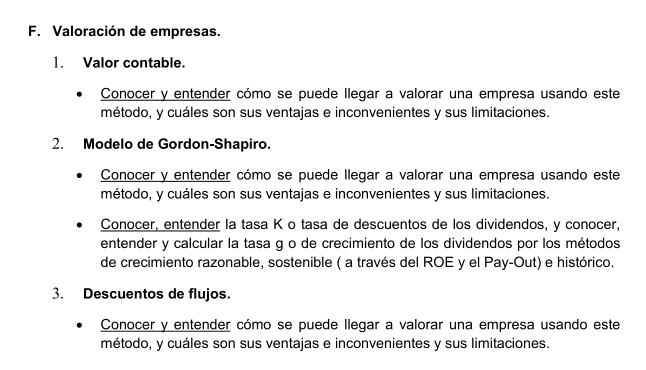
\includegraphics{./images/wacc.png}

Más información sobre el WACC en:
https://www.financlick.es/que-es-el-wacc-como-interpretarlo-n-81-es

\end{minipage}%
\end{tcolorbox}

\begin{center}\rule{0.5\linewidth}{0.5pt}\end{center}

\begin{enumerate}
\def\labelenumi{\arabic{enumi}.}
\setcounter{enumi}{88}
\tightlist
\item
  Si los dividendos anuales proyectados son 2,65 euros (2017), 3,08
  euros (2018) y 3,48 (2019). La tasa de rentabilidad requerida es de un
  14\% y la tasa de crecimiento anual de los dividendos esperada a
  partir de 2019 es un 8\%. El valor intrínseco por acción sería:
\end{enumerate}

\begin{enumerate}
\def\labelenumi{\alph{enumi})}
\item
  7 euros
\item
  69,5 euros
\item
  49,4 euros
\end{enumerate}

\begin{tcolorbox}[enhanced jigsaw, colback=white, colframe=quarto-callout-tip-color-frame, rightrule=.15mm, opacityback=0, toprule=.15mm, leftrule=.75mm, arc=.35mm, breakable, bottomrule=.15mm, left=2mm]
\begin{minipage}[t]{5.5mm}
\textcolor{quarto-callout-tip-color}{\faLightbulb}
\end{minipage}%
\begin{minipage}[t]{\textwidth - 5.5mm}

La respuesta \textbf{correcta es la c}.

El \textbf{valor intrínseco, precio teórico o valor fundamental de un
activo}, es el valor que se obtiene teniendo en cuenta todos los
componentes que rodean a un activo, incluyendo elementos tangibles e
intangibles. En ocasiones \textbf{también se conoce como valor real}.

Existen \textbf{múltiples métodos} de valoración de empresas, sin
embargo, \textbf{en el contexto del examen EFA de EFPA empleamos el
Modelo de Gordon}. Que valora el precio de la acción de una compañía en
función de los dividendos que va a repartir dicha compañía en el futuro.

Bien, para ello tenemos que plantear la referida fórmula,

\[P_O=\frac{D_1}{k-g}\]

donde,

\begin{itemize}
\item
  \(P_0\), es el precio teórico de la acción en el momento 0 (o valor
  actual).
\item
  \(D_1\), es el el dividendo que paga el título en el momento 1 (final
  del primer periodo).
\item
  \(k\), es la tasa de descuento o la rentabilidad mínima exigida por
  los accionistas a la empresa.
\item
  \(g\), es la tasa constante a la que crecerá el diviendo en cada
  periodo.
\end{itemize}

Notesé que en aquellos casos en los que desconocemos el valor de
\(D_1\), podemos hallar este a partir de \(D_0\) y la tasa a la que este
crece de forma anual a partir de ese momento cero:

\[D_1={D_O}\cdot ({1+g})\] De forma que, la fórmula anterior la podemos
expresar también como:

\[P_O=\frac{{D_O}\cdot ({1+g})}{k-g}\]

\[V_{int}=\frac{2.65}{1.14}+\frac{3.8}{1.14^2}+\frac{3.48}{1.14^3}+\frac{3.48\cdot1.08}{0.14-0.08}\cdot\frac{1}{1.14^3}=49.4\]

\end{minipage}%
\end{tcolorbox}

\begin{center}\rule{0.5\linewidth}{0.5pt}\end{center}

\begin{enumerate}
\def\labelenumi{\arabic{enumi}.}
\setcounter{enumi}{89}
\tightlist
\item
  El EVA:
\end{enumerate}

\begin{enumerate}
\def\labelenumi{\alph{enumi})}
\item
  Tiene en cuenta la tasa de crecimiento del Beneficio Neto
\item
  Tiene en cuenta la tasa de crecimiento del EBITDA
\item
  Tiene en cuenta la tasa de crecimiento de los dividendos
\item
  Tiene en cuenta la variación de los ingresos en el período de
  referencia
\end{enumerate}

\begin{tcolorbox}[enhanced jigsaw, colback=white, colframe=quarto-callout-tip-color-frame, rightrule=.15mm, opacityback=0, toprule=.15mm, leftrule=.75mm, arc=.35mm, breakable, bottomrule=.15mm, left=2mm]
\begin{minipage}[t]{5.5mm}
\textcolor{quarto-callout-tip-color}{\faLightbulb}
\end{minipage}%
\begin{minipage}[t]{\textwidth - 5.5mm}

La respuesta \textbf{correcta es la b}.

El Valor Económico Añadido (EVA) representa la productividad de todos
los factores empleados en la actividad empresarial. Es el remanente de
los ingresos una vez deducidos la totalidad de los gastos, incluidos el
coste de oportunidad del capital y los impuestos.

CÁLCULO:

\begin{itemize}
\item
  Resultado de actividades ordinarias antes de intereses y después de
  impuestos
\item
  Valor contable del activo × Coste promedio de financiación
\end{itemize}

\end{minipage}%
\end{tcolorbox}

\begin{center}\rule{0.5\linewidth}{0.5pt}\end{center}

\begin{enumerate}
\def\labelenumi{\arabic{enumi}.}
\setcounter{enumi}{90}
\tightlist
\item
  Utilizando el modelo de Gordon, se ha estimado que el valor teórico de
  una acción es 36,79. Dado que el dividendo es de 2,5 euros y que la
  tasa de rendimiento requerida por los accionistas es del 10\%, es
  posible afirmar que la tasa de crecimiento de los dividendos
  utilizados en el modelo es:
\end{enumerate}

\begin{enumerate}
\def\labelenumi{\alph{enumi}.}
\tightlist
\item
  4,10\%
\item
  3,20\%
\item
  2,05\%
\item
  5,00\%
\end{enumerate}

\begin{tcolorbox}[enhanced jigsaw, colback=white, colframe=quarto-callout-tip-color-frame, rightrule=.15mm, opacityback=0, toprule=.15mm, leftrule=.75mm, arc=.35mm, breakable, bottomrule=.15mm, left=2mm]
\begin{minipage}[t]{5.5mm}
\textcolor{quarto-callout-tip-color}{\faLightbulb}
\end{minipage}%
\begin{minipage}[t]{\textwidth - 5.5mm}

La respuesta \textbf{correcta es la b}.

Empleamos el descuento de dividendos crecientes a una tasa g (modelo de
Gordon)

\[P_O=\frac{D_1}{k-g}\] Sustituimos los valores del enunciado,

\[36.79=\frac{2.5}{0.10-g}\] y despejamos g,

\[g=0.03204\]

\end{minipage}%
\end{tcolorbox}

\begin{center}\rule{0.5\linewidth}{0.5pt}\end{center}

\hypertarget{mercado-de-divisas}{%
\section*{Mercado de Divisas}\label{mercado-de-divisas}}
\addcontentsline{toc}{section}{Mercado de Divisas}

\markright{Mercado de Divisas}

\begin{enumerate}
\def\labelenumi{\arabic{enumi}.}
\tightlist
\item
  La demanda de activos financieros denominados en euros por parte de
  los inversores extranjeros provocará:
\end{enumerate}

\begin{enumerate}
\def\labelenumi{\alph{enumi})}
\item
  Una apreciación del euro.
\item
  Una depreciación del euro.
\item
  La intervención del Banco Central Europeo.
\item
  No tiene ningún impacto.
\end{enumerate}

\begin{tcolorbox}[enhanced jigsaw, colback=white, colframe=quarto-callout-tip-color-frame, rightrule=.15mm, opacityback=0, toprule=.15mm, leftrule=.75mm, arc=.35mm, breakable, bottomrule=.15mm, left=2mm]
\begin{minipage}[t]{5.5mm}
\textcolor{quarto-callout-tip-color}{\faLightbulb}
\end{minipage}%
\begin{minipage}[t]{\textwidth - 5.5mm}

La respuesta \textbf{correcta es la a}.

El tipo de cambio de mercado de una divisa frente a otra varía en
función de la ley de la oferta y la demanda.Por tanto, la demanda de
activos financieros denominados en euros por parte de los inversores
extranjeros provocará una apreciación del euro. Cuando una divisa (al
igual que una mercancía) es escasa sube de precio (se aprecia), bien
porque es muy demandada o porque hay poca comparada con otras divisas.

\end{minipage}%
\end{tcolorbox}

\begin{center}\rule{0.5\linewidth}{0.5pt}\end{center}

\begin{enumerate}
\def\labelenumi{\arabic{enumi}.}
\setcounter{enumi}{1}
\tightlist
\item
  Un sistema cambiario flotante se caracteriza por:
\end{enumerate}

\begin{enumerate}
\def\labelenumi{\alph{enumi})}
\item
  El tipo de cambio lo fija la autoridad monetaria en función de la
  oferta y la demanda.
\item
  La existencia de bandas de flotación que acotan el rango d
  fluctuación.
\item
  La existencia del compromiso de intervención de la autoridad monetaria
  para defender la cotización
\item
  Ninguna de las anteriores
\end{enumerate}

\begin{tcolorbox}[enhanced jigsaw, colback=white, colframe=quarto-callout-tip-color-frame, rightrule=.15mm, opacityback=0, toprule=.15mm, leftrule=.75mm, arc=.35mm, breakable, bottomrule=.15mm, left=2mm]
\begin{minipage}[t]{5.5mm}
\textcolor{quarto-callout-tip-color}{\faLightbulb}
\end{minipage}%
\begin{minipage}[t]{\textwidth - 5.5mm}

La respuesta \textbf{correcta es la d}.

Un sistema de tipos de cambio flexible o flotante, es aquel en que los
que el tipo de cambio lo determina principalmente el mercado.

En algunos países con este sistema, el banco central interviene en el
mercado de cambios para para dar una cierta estabilidad a la divisa.
Esto es conocido como flotación sucia. Sin embargo, en otros, el banco
central casi nunca interviene.

La flotación ofrece al país la ventaja de mantener una política
monetaria independiente. En un país que establece un sistema de tipos de
cambio flotantes, el mercado de divisas y otros mercados financieros
deben estar suficientemente desarrollados para absorber los shocks sin
sufrir fluctuaciones importantes del tipo de cambio. También se
necesitan instrumentos financieros para cubrir los riesgos creados por
las fluctuaciones cambiarias.

\end{minipage}%
\end{tcolorbox}

\begin{center}\rule{0.5\linewidth}{0.5pt}\end{center}

\begin{enumerate}
\def\labelenumi{\arabic{enumi}.}
\setcounter{enumi}{2}
\tightlist
\item
  ¿Cuál de los siguientes medios de pago en moneda extranjera pueden
  considerarse divisas?:
\end{enumerate}

\begin{enumerate}
\def\labelenumi{\alph{enumi})}
\item
  Billetes de banco.
\item
  Saldos bancarios.
\item
  Instrumentos de movilización de los saldos bancarios: cheques y
  transferencias.
\item
  Todas las anteriores.
\end{enumerate}

\begin{tcolorbox}[enhanced jigsaw, colback=white, colframe=quarto-callout-tip-color-frame, rightrule=.15mm, opacityback=0, toprule=.15mm, leftrule=.75mm, arc=.35mm, breakable, bottomrule=.15mm, left=2mm]
\begin{minipage}[t]{5.5mm}
\textcolor{quarto-callout-tip-color}{\faLightbulb}
\end{minipage}%
\begin{minipage}[t]{\textwidth - 5.5mm}

La respuesta \textbf{correcta es la d}.

Pueden clasificarse como divisas los siguientes medios de pago en moneda
extranjera:

\begin{itemize}
\item
  Billetes de banco.
\item
  Cheques de viajero.
\item
  Saldos bancarios.
\item
  Instrumentos de movilización de los saldos bancarios: cheques y
  transferencias.
\end{itemize}

\end{minipage}%
\end{tcolorbox}

\begin{center}\rule{0.5\linewidth}{0.5pt}\end{center}

\begin{enumerate}
\def\labelenumi{\arabic{enumi}.}
\setcounter{enumi}{3}
\tightlist
\item
  Las principales funciones del mercado de divisas son:
\end{enumerate}

\begin{enumerate}
\def\labelenumi{\alph{enumi})}
\item
  Transferir poder adquisitivo de un país a otro.
\item
  Financiar el comercio internacional.
\item
  Propiciar cobertura frente al riesgo de cambio.
\item
  Todas las anteriores.
\end{enumerate}

\begin{tcolorbox}[enhanced jigsaw, colback=white, colframe=quarto-callout-tip-color-frame, rightrule=.15mm, opacityback=0, toprule=.15mm, leftrule=.75mm, arc=.35mm, breakable, bottomrule=.15mm, left=2mm]
\begin{minipage}[t]{5.5mm}
\textcolor{quarto-callout-tip-color}{\faLightbulb}
\end{minipage}%
\begin{minipage}[t]{\textwidth - 5.5mm}

La respuesta \textbf{correcta es la d}.

Las principales funciones del mercado de divisas son:

\begin{itemize}
\item
  Transferir poder adquisitivo de un país a otro.
\item
  Financiar el comercio internacional.
\item
  Propiciar cobertura frente al riesgo de cambio.
\end{itemize}

\end{minipage}%
\end{tcolorbox}

\begin{center}\rule{0.5\linewidth}{0.5pt}\end{center}

\begin{enumerate}
\def\labelenumi{\arabic{enumi}.}
\setcounter{enumi}{4}
\tightlist
\item
  Una operación de arbitraje se caracteriza por:
\end{enumerate}

\begin{enumerate}
\def\labelenumi{\alph{enumi})}
\item
  La toma de una posición direccional en el mercado.
\item
  La toma de una posición con el fin de eliminar el riesgo de cambio de
  una operación comercial.
\item
  La existencia de una ineficiencia en los precios que permite obtener
  un beneficio libre de riesgo.
\item
  Ninguna de las anteriores.
\end{enumerate}

\begin{tcolorbox}[enhanced jigsaw, colback=white, colframe=quarto-callout-tip-color-frame, rightrule=.15mm, opacityback=0, toprule=.15mm, leftrule=.75mm, arc=.35mm, breakable, bottomrule=.15mm, left=2mm]
\begin{minipage}[t]{5.5mm}
\textcolor{quarto-callout-tip-color}{\faLightbulb}
\end{minipage}%
\begin{minipage}[t]{\textwidth - 5.5mm}

La respuesta \textbf{correcta es la c}.

Como operativa en los mercados financieros, el arbitraje consiste en
realizar operaciones de compraventa en diferentes mercados y en un mismo
instante, con lo que se obtienen beneficios con operaciones exentas de
riesgo, pues estas operaciones se aprovechan de las distorsiones
temporales derivadas de las imperfecciones en los mecanismos de fijación
de precios. Su resultado es el equilibrio de los mercados.

\end{minipage}%
\end{tcolorbox}

\begin{center}\rule{0.5\linewidth}{0.5pt}\end{center}

\begin{enumerate}
\def\labelenumi{\arabic{enumi}.}
\setcounter{enumi}{5}
\tightlist
\item
  En una operación de compraventa de divisa a plazo:
\end{enumerate}

\begin{enumerate}
\def\labelenumi{\alph{enumi})}
\item
  Las dos partes adquieren la obligación de cumplir el compromiso
  pactado.
\item
  El tipo de cambio al que se realizará el intercambio de divisa se fija
  en el momento de la negociación.
\item
  La fecha de liquidación será posterior a la fecha spot.
\item
  Todas las anteriores.
\end{enumerate}

\begin{tcolorbox}[enhanced jigsaw, colback=white, colframe=quarto-callout-tip-color-frame, rightrule=.15mm, opacityback=0, toprule=.15mm, leftrule=.75mm, arc=.35mm, breakable, bottomrule=.15mm, left=2mm]
\begin{minipage}[t]{5.5mm}
\textcolor{quarto-callout-tip-color}{\faLightbulb}
\end{minipage}%
\begin{minipage}[t]{\textwidth - 5.5mm}

La respuesta \textbf{correcta es la d}.

El contrato a plazo de compraventa de divisas (contrato forward o seguro
de cambio) es un acuerdo en firme, no es opcional, sino de cumplimiento
obligatorio, por el que dos partes acuerdan intercambiar cierta cantidad
de divisas a un precio determinado y en una fecha futura.

La característica principal de este tipo de contrato es su flexibilidad:
las partes son las que negocian todos los términos del contrato. De esta
forma, las operaciones que se realizan bajo estas características son
operaciones ``a medida'' de las partes. Los vencimientos típicos son
múltiplos de un mes, dependiendo de las divisas el plazo máximo de
negociación. Se utilizan con tres fines: cobertura, especulación y
arbitraje.

\end{minipage}%
\end{tcolorbox}

\begin{center}\rule{0.5\linewidth}{0.5pt}\end{center}

\begin{enumerate}
\def\labelenumi{\arabic{enumi}.}
\setcounter{enumi}{6}
\tightlist
\item
  El mercado de divisas es del tipo:
\end{enumerate}

\begin{enumerate}
\def\labelenumi{\alph{enumi})}
\item
  Organizado y centralizado.
\item
  No organizado e interbancario.
\item
  Organizado siguiendo el modelo de las Bolsas de Valores.
\item
  Todas las anteriores.
\end{enumerate}

\begin{tcolorbox}[enhanced jigsaw, colback=white, colframe=quarto-callout-tip-color-frame, rightrule=.15mm, opacityback=0, toprule=.15mm, leftrule=.75mm, arc=.35mm, breakable, bottomrule=.15mm, left=2mm]
\begin{minipage}[t]{5.5mm}
\textcolor{quarto-callout-tip-color}{\faLightbulb}
\end{minipage}%
\begin{minipage}[t]{\textwidth - 5.5mm}

La respuesta \textbf{correcta es la b}.

El mercado de divisas es del tipo es un mercado no organizado e
interbancario.

\end{minipage}%
\end{tcolorbox}

\begin{center}\rule{0.5\linewidth}{0.5pt}\end{center}

\begin{enumerate}
\def\labelenumi{\arabic{enumi}.}
\setcounter{enumi}{7}
\tightlist
\item
  El mercado de eurodivisas lo podemos relacionar con:
\end{enumerate}

\begin{enumerate}
\def\labelenumi{\alph{enumi})}
\item
  Depósitos bancarios denominados en divisa.
\item
  Intrumentos financieros que pertenece al mercado monetario y de
  divisas.
\item
  Se negocian eurodepósitos y eurocréditos entre bancos y no bancos.
\item
  Todas las anteriores.
\end{enumerate}

\begin{tcolorbox}[enhanced jigsaw, colback=white, colframe=quarto-callout-tip-color-frame, rightrule=.15mm, opacityback=0, toprule=.15mm, leftrule=.75mm, arc=.35mm, breakable, bottomrule=.15mm, left=2mm]
\begin{minipage}[t]{5.5mm}
\textcolor{quarto-callout-tip-color}{\faLightbulb}
\end{minipage}%
\begin{minipage}[t]{\textwidth - 5.5mm}

La respuesta \textbf{correcta es la d}.

El mercado de eurodivisas o euromercado de dinero es el euromercado de
operaciones a corto plazo, es decir desde un día hasta un año.
Recientemente algunas de las operaciones se han alargado hasta año y
medio. El euromercado de divisas incluye el euromercado interbancario y
el euromercado de dinero no bancario. Y, en ellos, se intercambian
fondos, siempre en un país distinto de aquel en cuya divisa dichos
fondos están nominados.

\begin{itemize}
\item
  El euromercado interbancario, se refiere al mercado en que se
  gestionan los eurodepósitos y eurocréditos entre bancos a diferentes
  plazos entre un día y un año, pero predominantemente a un día. Al
  menos dos tercios de las operaciones del euromercado de dinero son
  operaciones interbancarias.
\item
  Los eurodepósitos y los eurocréditos pueden pertenecer al sector no
  bancario, es decir, a gobiernos, empresas y otras instituciones. En
  este caso se está hablando del euromercado de dinero no bancario.
\end{itemize}

\end{minipage}%
\end{tcolorbox}

\begin{center}\rule{0.5\linewidth}{0.5pt}\end{center}

\begin{enumerate}
\def\labelenumi{\arabic{enumi}.}
\setcounter{enumi}{8}
\tightlist
\item
  Un especulador en divisas tiene una expectativa de subida del dólar en
  los próximos 30 días:
\end{enumerate}

\begin{enumerate}
\def\labelenumi{\alph{enumi})}
\item
  Comprará dólares a futuro.
\item
  Comprará una opción de compra de dólares.
\item
  Venderá una opción de venta de dólares.
\item
  Todas son correctas
\end{enumerate}

\begin{tcolorbox}[enhanced jigsaw, colback=white, colframe=quarto-callout-tip-color-frame, rightrule=.15mm, opacityback=0, toprule=.15mm, leftrule=.75mm, arc=.35mm, breakable, bottomrule=.15mm, left=2mm]
\begin{minipage}[t]{5.5mm}
\textcolor{quarto-callout-tip-color}{\faLightbulb}
\end{minipage}%
\begin{minipage}[t]{\textwidth - 5.5mm}

La respuesta \textbf{correcta es la d}.

El especulador tiene una expectativa de subida del dólar en el futuro,
por tanto comprará dólares a futuro y/o una opción de compra de dólares
y venderá una opción de venta de dólares. Ya que todas estas estrategias
le permiten obtener un beneficio de cumplirse sus expectativas alcistas
sobre la divisa.

\end{minipage}%
\end{tcolorbox}

\begin{center}\rule{0.5\linewidth}{0.5pt}\end{center}

\begin{enumerate}
\def\labelenumi{\arabic{enumi}.}
\setcounter{enumi}{9}
\tightlist
\item
  Calcular el beneficio o pérdida obtenido por un especulador en el
  mercado cambiario si ha vendido dólares a futuro a un tipo de cambio
  de 1.31 y al vencimiento el tipo de cambio se sitúa en 1.33 dólares
  por euro. El nominal de la operación son 10.000 dólares:
\end{enumerate}

\begin{enumerate}
\def\labelenumi{\alph{enumi})}
\item
  114.8 euros
\item
  -114.8 euros
\item
  114.8 dólares
\item
  -114.8 dólares
\end{enumerate}

\begin{tcolorbox}[enhanced jigsaw, colback=white, colframe=quarto-callout-tip-color-frame, rightrule=.15mm, opacityback=0, toprule=.15mm, leftrule=.75mm, arc=.35mm, breakable, bottomrule=.15mm, left=2mm]
\begin{minipage}[t]{5.5mm}
\textcolor{quarto-callout-tip-color}{\faLightbulb}
\end{minipage}%
\begin{minipage}[t]{\textwidth - 5.5mm}

La respuesta \textbf{correcta es la a}.

\[B/P=N\cdot (P_{venta}-P_{compra})\] Donde,

\begin{itemize}
\item
  \(B/P\), es el beneficio o pérdida obtenido por un especulador.
\item
  \(N\), es el nominal de la operación.
\item
  \(P_{venta}\), es el precio de venta a futuro.
\item
  \(P_{compra}\), es el precio de compra de contado en el momento
  futuro.
\end{itemize}

\[B/P=10000\cdot\left(\frac{1}{1.31}-\frac{1}{1.33}\right)=114.7907\]

\end{minipage}%
\end{tcolorbox}

\begin{center}\rule{0.5\linewidth}{0.5pt}\end{center}

\begin{enumerate}
\def\labelenumi{\arabic{enumi}.}
\setcounter{enumi}{10}
\tightlist
\item
  El incremento de las exportaciones de un país con un sistema cambiario
  libre introduce presión en el tipo de cambio:
\end{enumerate}

\begin{enumerate}
\def\labelenumi{\alph{enumi})}
\item
  Apreciando su moneda
\item
  Depreciando su moneda
\item
  No tiene ningún impacto
\end{enumerate}

\begin{enumerate}
\def\labelenumi{\Alph{enumi})}
\setcounter{enumi}{3}
\tightlist
\item
  Dependerá de los tipos de interés del país receptor de las
  importacones
\end{enumerate}

\begin{tcolorbox}[enhanced jigsaw, colback=white, colframe=quarto-callout-tip-color-frame, rightrule=.15mm, opacityback=0, toprule=.15mm, leftrule=.75mm, arc=.35mm, breakable, bottomrule=.15mm, left=2mm]
\begin{minipage}[t]{5.5mm}
\textcolor{quarto-callout-tip-color}{\faLightbulb}
\end{minipage}%
\begin{minipage}[t]{\textwidth - 5.5mm}

La respuesta \textbf{correcta es la a}.

De acuerdo con la teoría económica, las exportaciones tienen una
relación directa con el tipo de cambio. Es decir, si las exportaciones
de un país aumentan la moneda se aprecia, y viceversa. Esto se debe a
que la demanda de moneda local para llevar a cabo las compras de los
bienes y servicios demandados generarán una presión al alza en la
cotización de esa moneda en el mercado de divisas.

\end{minipage}%
\end{tcolorbox}

\begin{center}\rule{0.5\linewidth}{0.5pt}\end{center}

\begin{enumerate}
\def\labelenumi{\arabic{enumi}.}
\setcounter{enumi}{11}
\tightlist
\item
  Una operación de arbitraje se caracteriza por:
\end{enumerate}

\begin{enumerate}
\def\labelenumi{\alph{enumi})}
\item
  El mismo activo no se transmite al mismo precio en distintos mercados.
\item
  Un activo con un precio conocido en el futuro no se vende hoy a su
  precio futuro descontado a la tasa de interés libre de riesgo.
\item
  La existencia de ineficiencia en los precios de los activos que
  permite obtener un beneficio libre de riesgo.
\item
  Todas las anteriores.
\end{enumerate}

\begin{tcolorbox}[enhanced jigsaw, colback=white, colframe=quarto-callout-tip-color-frame, rightrule=.15mm, opacityback=0, toprule=.15mm, leftrule=.75mm, arc=.35mm, breakable, bottomrule=.15mm, left=2mm]
\begin{minipage}[t]{5.5mm}
\textcolor{quarto-callout-tip-color}{\faLightbulb}
\end{minipage}%
\begin{minipage}[t]{\textwidth - 5.5mm}

La respuesta \textbf{correcta es la d}.

El arbitraje es la existencia de ineficiencia en los precios de los
activos que permiten obtener un beneficio libre de riesgo. Este será
posible cuando al menos una de las siguientes condiciones se cumple:

\begin{itemize}
\item
  El mismo activo no se transmite al mismo precio en distintos mercados.
\item
  Dos activos que producen el mismo flujo de efectivo no se transmiten
  al mismo precio.
\item
  Un activo con un precio conocido en el futuro no se vende hoy a su
  precio futuro descontado a la tasa de interés libre de riesgo.
\end{itemize}

\end{minipage}%
\end{tcolorbox}

\begin{center}\rule{0.5\linewidth}{0.5pt}\end{center}

\begin{enumerate}
\def\labelenumi{\arabic{enumi}.}
\setcounter{enumi}{12}
\tightlist
\item
  Si el tipo de cambio €/\$ pasa de 0.95 dólares por euro a 0.90 dólares
  por euros:
\end{enumerate}

\begin{enumerate}
\def\labelenumi{\alph{enumi})}
\item
  Se estará produciendo una apreciación del dólar
\item
  Se estará produciendo una depreciación del dólar
\item
  Se está produciendo una apreciación del euro
\item
  Son correctas la b y c
\end{enumerate}

\begin{tcolorbox}[enhanced jigsaw, colback=white, colframe=quarto-callout-tip-color-frame, rightrule=.15mm, opacityback=0, toprule=.15mm, leftrule=.75mm, arc=.35mm, breakable, bottomrule=.15mm, left=2mm]
\begin{minipage}[t]{5.5mm}
\textcolor{quarto-callout-tip-color}{\faLightbulb}
\end{minipage}%
\begin{minipage}[t]{\textwidth - 5.5mm}

La respuesta \textbf{correcta es la a}.

Se estará produciendo una apreciación del dólar, ya que ahora
recibiremos menos dólares por un euro.

\end{minipage}%
\end{tcolorbox}

\begin{center}\rule{0.5\linewidth}{0.5pt}\end{center}

\begin{enumerate}
\def\labelenumi{\arabic{enumi}.}
\setcounter{enumi}{13}
\tightlist
\item
  Si la cotización del €/Yen nos presenta los siguientes precios de
  compra/venta:
\end{enumerate}

\begin{longtable}[]{@{}cc@{}}
\toprule()
BID & OFFER \\
\midrule()
\endhead
162.60 & 162.71 \\
\bottomrule()
\end{longtable}

\begin{enumerate}
\def\labelenumi{\alph{enumi})}
\item
  Podremos comprar dólares a 180 yenes.
\item
  Podremos comprar yenes a 162.71.
\item
  Podremos comprar euros a 162.71.
\item
  Ninguna de las anteriores.
\end{enumerate}

\begin{tcolorbox}[enhanced jigsaw, colback=white, colframe=quarto-callout-tip-color-frame, rightrule=.15mm, opacityback=0, toprule=.15mm, leftrule=.75mm, arc=.35mm, breakable, bottomrule=.15mm, left=2mm]
\begin{minipage}[t]{5.5mm}
\textcolor{quarto-callout-tip-color}{\faLightbulb}
\end{minipage}%
\begin{minipage}[t]{\textwidth - 5.5mm}

La respuesta \textbf{correcta es la c}.

El término ``bid'' hace referencia al precio de compra, mientras que
``offer'' harían referencia al precio de venta. Pero claro, en este caso
el precio de venta es nuestro precio de compra. Es decir, cuando vas a
comprar y te dan la diferencia existente entre ambos precios (spread),
cojeremos siempre el más caro ya que es en esa diferencia donde se
encuentra el beneficio del operador que vende.

\end{minipage}%
\end{tcolorbox}

\begin{center}\rule{0.5\linewidth}{0.5pt}\end{center}

\begin{enumerate}
\def\labelenumi{\arabic{enumi}.}
\setcounter{enumi}{14}
\tightlist
\item
  El mayor volumen de operaciones en el mercado de divisas es el
  realizado por:
\end{enumerate}

\begin{enumerate}
\def\labelenumi{\alph{enumi})}
\item
  Las operaciones de comercio internacional.
\item
  Las operaciones de cambio de los turistas y viajeros.
\item
  Las operaciones de especulación de los bancos comerciales y de
  deinversión.
\item
  Las operaciones de cobertura a plazo.
\end{enumerate}

\begin{tcolorbox}[enhanced jigsaw, colback=white, colframe=quarto-callout-tip-color-frame, rightrule=.15mm, opacityback=0, toprule=.15mm, leftrule=.75mm, arc=.35mm, breakable, bottomrule=.15mm, left=2mm]
\begin{minipage}[t]{5.5mm}
\textcolor{quarto-callout-tip-color}{\faLightbulb}
\end{minipage}%
\begin{minipage}[t]{\textwidth - 5.5mm}

La respuesta \textbf{correcta es la c}.

El mercado de divisas, FX o mercado Forex es el mercado en el que se
negocian las monedas de los distintos países. El volumen de divisas
negociado diariamente supera los 5 billones de dólares, lo que le
convierte en el mercado financiero de mayor volumen y más líquido a
nivel mundial. Los principales operadores en el mercado de divisas son
los bancos comerciales y de de inversión.

\end{minipage}%
\end{tcolorbox}

\begin{center}\rule{0.5\linewidth}{0.5pt}\end{center}

\begin{enumerate}
\def\labelenumi{\arabic{enumi}.}
\setcounter{enumi}{15}
\tightlist
\item
  Un importador español de químicos procedentes de EE.UU podrá cubrir el
  riesgo cambiario de su operativa:
\end{enumerate}

\begin{enumerate}
\def\labelenumi{\alph{enumi})}
\item
  Comprando euros y cambiarlos a dólares amareicanos.
\item
  Comprando dólares australianos a futuro.
\item
  Comprandon un seguro de cambio mediante el cual intercambiar una
  cantidad de divisa a un precio fijado en una fecha futura.
\item
  Ninguna de las anteriores.
\end{enumerate}

\begin{tcolorbox}[enhanced jigsaw, colback=white, colframe=quarto-callout-tip-color-frame, rightrule=.15mm, opacityback=0, toprule=.15mm, leftrule=.75mm, arc=.35mm, breakable, bottomrule=.15mm, left=2mm]
\begin{minipage}[t]{5.5mm}
\textcolor{quarto-callout-tip-color}{\faLightbulb}
\end{minipage}%
\begin{minipage}[t]{\textwidth - 5.5mm}

La respuesta \textbf{correcta es la c}.

Un seguro de cambio le garantizará un precio fijo de compra,
independientemente de la evolución de la cotización del EUR/USD. El
cambio fijado puede ser superior (divisa con premio) o bien inferior
(divisa con descuento) al del día de su contratación.

Con el seguro de cambio, al vencimiento, comprará el nominal establecido
al tipo fijado. El seguro de cambio no le permite beneficiarse de las
posibles fluctuaciones favorables de la divisa.

\end{minipage}%
\end{tcolorbox}

\begin{center}\rule{0.5\linewidth}{0.5pt}\end{center}

\begin{enumerate}
\def\labelenumi{\arabic{enumi}.}
\setcounter{enumi}{16}
\tightlist
\item
  La Paridad Cubierta de Intereses:
\end{enumerate}

\begin{enumerate}
\def\labelenumi{\alph{enumi})}
\item
  Es función de las expectativas sobre la evolución del tipo de cambio.
\item
  Es función de las expectativas sobre la evolución de los tipos de
  interés.
\item
  Determina el tipo de cambio a plazo.
\item
  Ninguna es correcta.
\end{enumerate}

\begin{tcolorbox}[enhanced jigsaw, colback=white, colframe=quarto-callout-tip-color-frame, rightrule=.15mm, opacityback=0, toprule=.15mm, leftrule=.75mm, arc=.35mm, breakable, bottomrule=.15mm, left=2mm]
\begin{minipage}[t]{5.5mm}
\textcolor{quarto-callout-tip-color}{\faLightbulb}
\end{minipage}%
\begin{minipage}[t]{\textwidth - 5.5mm}

La respuesta \textbf{correcta es la c}.

La paridad de tasas de interés es una condición que representa un estado
de equilibrio en el que los inversores son indiferentes a las tasas de
interés disponibles en depósitos bancarios en dos países diferentes, sin
arbitraje.

El hecho de que esta condición no siempre se cumpla permite
oportunidades potenciales de obtener ganancias sin riesgo con
operaciones de arbitraje de tasas de interés.

La paridad de tasas de interés se base en dos supuestos centrales, la
movilidad del capital y la sustitución perfecta de los activos
nacionales y extranjeros. Teniendo en cuenta el equilibrio del mercado
de divisas, la condición de paridad de tipos de interés implica que el
rendimiento esperado de los activos domésticos será igual al rendimiento
esperado de los activos en moneda extranjera ajustado por el tipo de
cambio. Los inversores a continuación, no pueden obtener beneficios de
arbitraje por los préstamos en un país con una tasa de interés más baja,
el intercambio de moneda extranjera, y la inversión en un país
extranjero con una tasa de interés más alta, debido a las ganancias o
pérdidas de intercambio de vuelta a su moneda nacional en el
vencimiento. La paridad de tasas de interés adquiere dos formas
diferentes:

\begin{itemize}
\item
  la paridad de tasas de interés sin cobertura se refiere a la condición
  de paridad en los que la exposición al riesgo de cambio (cambios no
  anticipados en los tipos de cambio) es desinhibida,
\item
  \textbf{la paridad de la tasa de interés cubierta se refiere a la
  condición en la que se ha utilizado un contrato forward para cubrir
  (eliminar la exposición) el riesgo de tipo de cambio}.
\end{itemize}

\end{minipage}%
\end{tcolorbox}

\begin{center}\rule{0.5\linewidth}{0.5pt}\end{center}

\begin{enumerate}
\def\labelenumi{\arabic{enumi}.}
\setcounter{enumi}{17}
\tightlist
\item
  En una situación de Paridad Cubierta de Intereses:
\end{enumerate}

\begin{enumerate}
\def\labelenumi{\alph{enumi})}
\item
  No es posible obtener un beneficio libre de riesgo.
\item
  El tipo de cambio a plazo es igual al tipo de cambio a contado.
\item
  Es indiferente realizar una inversión descubierta en dólares o una
  inversión en euros.
\item
  Ninguna es correcta.
\end{enumerate}

\begin{tcolorbox}[enhanced jigsaw, colback=white, colframe=quarto-callout-tip-color-frame, rightrule=.15mm, opacityback=0, toprule=.15mm, leftrule=.75mm, arc=.35mm, breakable, bottomrule=.15mm, left=2mm]
\begin{minipage}[t]{5.5mm}
\textcolor{quarto-callout-tip-color}{\faLightbulb}
\end{minipage}%
\begin{minipage}[t]{\textwidth - 5.5mm}

La respuesta \textbf{correcta es la a}.

La paridad de tasas de interés es una condición que representa un estado
de equilibrio en el que los inversores son indiferentes a las tasas de
interés disponibles en depósitos bancarios en dos países diferentes,
\textbf{sin arbitraje}.

El hecho de que esta condición no siempre se cumpla permite
oportunidades potenciales de obtener ganancias sin riesgo con
operaciones de arbitraje de tasas de interés.

La paridad de tasas de interés se base en dos supuestos centrales, la
movilidad del capital y la sustitución perfecta de los activos
nacionales y extranjeros. Teniendo en cuenta el equilibrio del mercado
de divisas, la condición de paridad de tipos de interés implica que el
rendimiento esperado de los activos domésticos será igual al rendimiento
esperado de los activos en moneda extranjera ajustado por el tipo de
cambio. Los inversores a continuación, no pueden obtener beneficios de
arbitraje por los préstamos en un país con una tasa de interés más baja,
el intercambio de moneda extranjera, y la inversión en un país
extranjero con una tasa de interés más alta, debido a las ganancias o
pérdidas de intercambio de vuelta a su moneda nacional en el
vencimiento. La paridad de tasas de interés adquiere dos formas
diferentes:

\begin{itemize}
\item
  la paridad de tasas de interés sin cobertura se refiere a la condición
  de paridad en los que la exposición al riesgo de cambio (cambios no
  anticipados en los tipos de cambio) es desinhibida,
\item
  la paridad de la tasa de interés cubierta se refiere a la condición en
  la que se ha utilizado un contrato forward para cubrir (eliminar la
  exposición) el riesgo de tipo de cambio.
\end{itemize}

\end{minipage}%
\end{tcolorbox}

\begin{center}\rule{0.5\linewidth}{0.5pt}\end{center}

\begin{enumerate}
\def\labelenumi{\arabic{enumi}.}
\setcounter{enumi}{18}
\tightlist
\item
  El mercado de divisas puede considerarse, en términos generales,:
\end{enumerate}

\begin{enumerate}
\def\labelenumi{\alph{enumi})}
\item
  Un mercado organizado.
\item
  Un mercado OTC.
\item
  Un mercado donde los productos y plazos están estandarizados.
\item
  Un mercado primario por su importancia.
\end{enumerate}

\begin{tcolorbox}[enhanced jigsaw, colback=white, colframe=quarto-callout-tip-color-frame, rightrule=.15mm, opacityback=0, toprule=.15mm, leftrule=.75mm, arc=.35mm, breakable, bottomrule=.15mm, left=2mm]
\begin{minipage}[t]{5.5mm}
\textcolor{quarto-callout-tip-color}{\faLightbulb}
\end{minipage}%
\begin{minipage}[t]{\textwidth - 5.5mm}

La respuesta \textbf{correcta es la b}.

A diferencia de otros mercados financieros como el mercado de acciones,
el mercado de divisas no cuenta con una ubicación fija como las mayores
bolsas del mundo. A este tipo de mercados se les conoce como OTC (Over
The Counter). Las transacciones se realizan de forma independiente
alrededor de todo el mundo, principalmente a través de Internet.

\end{minipage}%
\end{tcolorbox}

\begin{center}\rule{0.5\linewidth}{0.5pt}\end{center}

\begin{enumerate}
\def\labelenumi{\arabic{enumi}.}
\setcounter{enumi}{19}
\tightlist
\item
  El tipo de cambio al contado evoluciona desde los GBP/USD 1,7800 hasta
  los GBP/USD 1,8100. En este caso, podemos decir que:
\end{enumerate}

\begin{enumerate}
\def\labelenumi{\alph{enumi})}
\item
  El dólar se ha apreciado frente a la libra.
\item
  El dólar se ha depreciado frente a la libra.
\item
  El tipo de interés en libras es mayor que el tipo de interés en
  dólares.
\item
  La b) y la c) son correctas.
\end{enumerate}

\begin{tcolorbox}[enhanced jigsaw, colback=white, colframe=quarto-callout-tip-color-frame, rightrule=.15mm, opacityback=0, toprule=.15mm, leftrule=.75mm, arc=.35mm, breakable, bottomrule=.15mm, left=2mm]
\begin{minipage}[t]{5.5mm}
\textcolor{quarto-callout-tip-color}{\faLightbulb}
\end{minipage}%
\begin{minipage}[t]{\textwidth - 5.5mm}

La respuesta \textbf{correcta es la d}.

Según los datos que nos dan, y la teoría de de la paridad de los tipos
de interés (TPTI), podemos afirmar que el tipo de interés en libras es
mayor que el tipo de interés en dólares. Ya que la depreciación del tipo
de cambio en una moneda a plazo (dólar), con respecto a otra que sirve
de referencia (libra), se explica por las diferencias en los tipos de
interés entre dichas monedas.

\end{minipage}%
\end{tcolorbox}

\begin{center}\rule{0.5\linewidth}{0.5pt}\end{center}

\begin{enumerate}
\def\labelenumi{\arabic{enumi}.}
\setcounter{enumi}{21}
\tightlist
\item
  Si la tasa de interés interbancario a 3 meses del euro y del dólar son
  2,25\% y 1,25\% respectivamente y el tipo de cambio spot €/\$ es de
  1,15. El tipo de cambio a plazo a tres meses será:
\end{enumerate}

\begin{enumerate}
\def\labelenumi{\alph{enumi})}
\item
  €/\$ 1,147.
\item
  €/\$ 1,578.
\item
  €/\$ 0,935.
\item
  Ninguna de las anteriores.
\end{enumerate}

\begin{tcolorbox}[enhanced jigsaw, colback=white, colframe=quarto-callout-tip-color-frame, rightrule=.15mm, opacityback=0, toprule=.15mm, leftrule=.75mm, arc=.35mm, breakable, bottomrule=.15mm, left=2mm]
\begin{minipage}[t]{5.5mm}
\textcolor{quarto-callout-tip-color}{\faLightbulb}
\end{minipage}%
\begin{minipage}[t]{\textwidth - 5.5mm}

La respuesta \textbf{correcta es la a}.

El tipo forward será:

\[F_{local/divisa}=S_{local/divisa}\cdot{}\frac{1+i_{divisa}\cdot \frac{n}{base}}{1+i_{local}\cdot \frac{n}{base}}\]
Que al sustituir y calcular,

\[F_{euro/dolar}=1.15\cdot\frac{\left(1+0.0125\cdot\frac{1}{4}\right)}{\left(1+0.025\cdot\frac{1}{4}\right)}=1.147\]

\end{minipage}%
\end{tcolorbox}

\begin{center}\rule{0.5\linewidth}{0.5pt}\end{center}

\begin{enumerate}
\def\labelenumi{\arabic{enumi}.}
\setcounter{enumi}{22}
\tightlist
\item
  Un inversor español tiene en su cartera una acción británica. A lo
  largo del primer año, el título pierde el 10\% de su valor mientras
  que la libra esterlina : se aprecia en un 10 \% con respecto al euro.
  ¿Cuál es la rentabilidad, en euros, conseguida por el inversor?:
\end{enumerate}

\begin{enumerate}
\def\labelenumi{\alph{enumi})}
\item
  -10\%.
\item
  0\%.
\item
  +1\%.
\item
  -1\%.
\end{enumerate}

\begin{tcolorbox}[enhanced jigsaw, colback=white, colframe=quarto-callout-tip-color-frame, rightrule=.15mm, opacityback=0, toprule=.15mm, leftrule=.75mm, arc=.35mm, breakable, bottomrule=.15mm, left=2mm]
\begin{minipage}[t]{5.5mm}
\textcolor{quarto-callout-tip-color}{\faLightbulb}
\end{minipage}%
\begin{minipage}[t]{\textwidth - 5.5mm}

La respuesta \textbf{correcta es la d}.

Nos piden calcular la TIR de esta operación financiera.

\[\left(1+TIR\right)=\left(1+i_1\right)\cdot\left(1+i_2\right)\]

Donde,

\begin{itemize}
\item
  \(TIR\), va ha ser la Tasa de Rentabilidad Interna obteniada ``a lo
  largo del primer año''.
\item
  \(i_1\), será la rentabilidad obtenida por la revalorización del
  activo.
\item
  \(i_2\), será la rentabilidad obtenida por la revalorización de la
  divisa.
\end{itemize}

Ahora despejamos la TIR, sustituimos y calculamos:

\[TIR=\left[((1-0.10)\cdot(1+0.10))-1\right]=-0.01(-1\%)\]

\end{minipage}%
\end{tcolorbox}

\begin{center}\rule{0.5\linewidth}{0.5pt}\end{center}

\begin{enumerate}
\def\labelenumi{\arabic{enumi}.}
\setcounter{enumi}{23}
\tightlist
\item
  Sean dos activos A y B, el primero con un rendimiento del 8\% a 1 año
  y el B con un rendimiento del 10\% a dos años. ¿Cuál será el tipo
  forward o implícito para una inversión a un año, dentro de un año?:
\end{enumerate}

\begin{enumerate}
\def\labelenumi{\alph{enumi})}
\item
  10\%.
\item
  12\%.
\item
  11,5\%.
\item
  Ninguna de los anteriores.
\end{enumerate}

\begin{tcolorbox}[enhanced jigsaw, colback=white, colframe=quarto-callout-tip-color-frame, rightrule=.15mm, opacityback=0, toprule=.15mm, leftrule=.75mm, arc=.35mm, breakable, bottomrule=.15mm, left=2mm]
\begin{minipage}[t]{5.5mm}
\textcolor{quarto-callout-tip-color}{\faLightbulb}
\end{minipage}%
\begin{minipage}[t]{\textwidth - 5.5mm}

La respuesta \textbf{correcta es la b}.

Simplemente aplicando el tipo de interés implícito de un años dentro de
un año.

\[(1+_{0}S_{1})\cdot(1+f_{1,2})=(1+_{0}S_{2})^{2}\] Despejamos el tipo
de interés implícito o \emph{forward} \(f_{1,2}\),

\[f_{1,2}=\frac{(1+0.10)^{2} }{(1+0.08) }-1=12.03(12\%)\] Sustituimos y
calculamos,

\[f_{1,2}=\frac{(1+_{0}S_{1}) }{ (1+_{0}S_{2})^{2}}-1\]

\end{minipage}%
\end{tcolorbox}

\begin{center}\rule{0.5\linewidth}{0.5pt}\end{center}

\begin{enumerate}
\def\labelenumi{\arabic{enumi}.}
\setcounter{enumi}{24}
\tightlist
\item
  Si la tasa de interés interbancario a 6 meses del euro y del dólar son
  3,5\% y 5,0\% respectivamente, y el tipo de cambio spot EUR/USD es de
  1,2534 dólares por euro. El tipo de cambio a plazo a seis meses será:
\end{enumerate}

\begin{enumerate}
\def\labelenumi{\alph{enumi})}
\item
  EUR/USD 1,2626.
\item
  EUR/USD 1,2442.
\item
  EUR/USD 1,2587.
\item
  La información de que dispongo es insuficiente para responder a la
  pregunta.
\end{enumerate}

\begin{tcolorbox}[enhanced jigsaw, colback=white, colframe=quarto-callout-tip-color-frame, rightrule=.15mm, opacityback=0, toprule=.15mm, leftrule=.75mm, arc=.35mm, breakable, bottomrule=.15mm, left=2mm]
\begin{minipage}[t]{5.5mm}
\textcolor{quarto-callout-tip-color}{\faLightbulb}
\end{minipage}%
\begin{minipage}[t]{\textwidth - 5.5mm}

La respuesta \textbf{correcta es la a}.

1º Para resolver esta pregunta tenemos que aplicar la siguiente fórmula,
que muestra la relación existente entre los tipos de cambio a plazo y
los tipos de cambio al contado. Que de una forma genérica queda como
sigue:

\[{ F }_{ Base/Referencia }={ S }_{ Base/Referencia }\cdot \frac { 1+{ i }_{ Referencia }\cdot \frac { n }{ Base }  }{ 1+{ i }_{ Base }\cdot \frac { n }{ Base }  } \]

Y, para nuestro caso sería:

\[{ F }_{ EUR/USD }={ S }_{ EUR/USD }\cdot \frac { 1+{ i }_{ USD }\cdot\frac { n }{ Base }  }{ 1+{ i }_{ EUR }\cdot \frac { n }{ Base }  } \]

Donde:

\begin{itemize}
\tightlist
\item
  \({ F }_{ EUR/USD }\) : tipo de cambio a plazo o \emph{forward} de n
  días (meses, años, etc.) expresado de forma indirecta
\item
  \({ S }_{ EUR/USD }\) : tipo de cambio a contado o \emph{spot}
  expresado de forma indirecta
\item
  \({ i }_{USD}\) : tipo de interés sobre la divisa (dólar)
\item
  \({ i }_{EUR}\) : tipo de interés sobre la moneda local (euro)
\item
  \(n\) : número de días que trancurren del contrato a plazo
\end{itemize}

2º Sustituimos los datos en la ecuación anterior,

\[ { F }_{ USD/EUR }=1,2534\cdot \frac { 1+0,05\frac { 6 }{ 12 }  }{ 1+0.035\frac { 6 }{ 12 }  }=1.262639 \]

\end{minipage}%
\end{tcolorbox}

\begin{center}\rule{0.5\linewidth}{0.5pt}\end{center}

\begin{enumerate}
\def\labelenumi{\arabic{enumi}.}
\setcounter{enumi}{25}
\tightlist
\item
  Una operación de contado en divisas (suponiendo todos los días
  hábiles) es aquella que:
\end{enumerate}

\begin{enumerate}
\def\labelenumi{\alph{enumi}.}
\item
  Siempre se liquida dos días hábiles posteriores a la fecha de
  contratación.
\item
  Si se contrata el miércoles se podrá liquidar el viernes.
\item
  Si se contrata un jueves se liquidará el mismo día de la semana
  siguiente.
\item
  Ninguna de las anteriores.
\end{enumerate}

\begin{tcolorbox}[enhanced jigsaw, colback=white, colframe=quarto-callout-tip-color-frame, rightrule=.15mm, opacityback=0, toprule=.15mm, leftrule=.75mm, arc=.35mm, breakable, bottomrule=.15mm, left=2mm]
\begin{minipage}[t]{5.5mm}
\textcolor{quarto-callout-tip-color}{\faLightbulb}
\end{minipage}%
\begin{minipage}[t]{\textwidth - 5.5mm}

La respuesta \textbf{correcta es la b}.

Operaciones de \textbf{contado (spot)} son aquellas operaciones de
compra y venta de divisas, tanto contra euros como contra otras divisas,
cuando \textbf{entre la fecha de contratación y la de valor no han
transcurrido más de dos días hábiles}.

Cualquier transacción en el mercado de divisas que suponga una
liquidación en un plazo \textbf{superior a dos días hábiles después de
haberse contratado} la operación es denominada \textbf{operación a plazo
(forward)}.

\end{minipage}%
\end{tcolorbox}

\begin{center}\rule{0.5\linewidth}{0.5pt}\end{center}

\begin{enumerate}
\def\labelenumi{\arabic{enumi}.}
\setcounter{enumi}{26}
\tightlist
\item
  Los puntos swap son:
\end{enumerate}

\begin{enumerate}
\def\labelenumi{\alph{enumi}.}
\item
  El diferencial sobre el LIBOR del tipo de interés de una moneda.
\item
  La diferencia entre los tipos de interés de las dos monedas.
\item
  La diferencia entre el tipo de cambio a plazo y el tipo de cambio al
  contado.
\item
  Son ciertas b y c.
\end{enumerate}

\begin{tcolorbox}[enhanced jigsaw, colback=white, colframe=quarto-callout-tip-color-frame, rightrule=.15mm, opacityback=0, toprule=.15mm, leftrule=.75mm, arc=.35mm, breakable, bottomrule=.15mm, left=2mm]
\begin{minipage}[t]{5.5mm}
\textcolor{quarto-callout-tip-color}{\faLightbulb}
\end{minipage}%
\begin{minipage}[t]{\textwidth - 5.5mm}

La respuesta \textbf{correcta es la c}.

Los puntos swap (o también llamados puntos forward. son la diferencia
entre el tipo de cambio a plazo (forward. y el tipo de cambio al contado
(spot).

\end{minipage}%
\end{tcolorbox}

\begin{center}\rule{0.5\linewidth}{0.5pt}\end{center}

\begin{enumerate}
\def\labelenumi{\arabic{enumi}.}
\setcounter{enumi}{27}
\tightlist
\item
  El tipo al contado EUR/USD es 1,30 usd por 1 euro y los tipos de
  interés a vencimiento del forward del USD y del EUR son
  respectivamente el 3\% y el 2\%. Indique cuál de las siguientes
  respuestas NO corresponde con seguridad con la cotización del tipo de
  cambio forward:
\end{enumerate}

\begin{enumerate}
\def\labelenumi{\alph{enumi}.}
\item
  1,2936
\item
  1,3064
\item
  1,3085
\item
  1,3110
\end{enumerate}

\begin{tcolorbox}[enhanced jigsaw, colback=white, colframe=quarto-callout-tip-color-frame, rightrule=.15mm, opacityback=0, toprule=.15mm, leftrule=.75mm, arc=.35mm, breakable, bottomrule=.15mm, left=2mm]
\begin{minipage}[t]{5.5mm}
\textcolor{quarto-callout-tip-color}{\faLightbulb}
\end{minipage}%
\begin{minipage}[t]{\textwidth - 5.5mm}

La respuesta \textbf{correcta es la a}.

Para calcular el tipo de cambio forward planteamos:

\[F_{EUR/USD}=S_{EUR/USD}\frac{1+i_{USD}\cdot n}{1+i_{EUR}\cdot n}\]
Como el tipo de interés del USD (3\%) es mayor que el tipo de interés
del EUR (2\%) el forward será mayor que el spot. Si el spot EURUSD es
1,3000 el forward NO puede ser 1,2936 (a).

\end{minipage}%
\end{tcolorbox}

\begin{center}\rule{0.5\linewidth}{0.5pt}\end{center}

\begin{enumerate}
\def\labelenumi{\arabic{enumi}.}
\setcounter{enumi}{28}
\tightlist
\item
  Un seguro de cambio:
\end{enumerate}

\begin{enumerate}
\def\labelenumi{\alph{enumi}.}
\item
  Vincula a ambas partes contratantes.
\item
  La cámara de compensación que regula en España este tipo de contratos
  es MEFF
\item
  Es una operación de compra o venta de divisas al contado.
\item
  Reduce pero no elimina el riesgo de tipo de cambio.
\end{enumerate}

\begin{tcolorbox}[enhanced jigsaw, colback=white, colframe=quarto-callout-tip-color-frame, rightrule=.15mm, opacityback=0, toprule=.15mm, leftrule=.75mm, arc=.35mm, breakable, bottomrule=.15mm, left=2mm]
\begin{minipage}[t]{5.5mm}
\textcolor{quarto-callout-tip-color}{\faLightbulb}
\end{minipage}%
\begin{minipage}[t]{\textwidth - 5.5mm}

La respuesta \textbf{correcta es la a}.

Un seguro de cambio es un compromiso mediante el cual el cliente y el
banco se obligan mutuamente a intercambiar una cantidad de divisa a un
precio fijado en una fecha futura.

\end{minipage}%
\end{tcolorbox}

\begin{center}\rule{0.5\linewidth}{0.5pt}\end{center}

\begin{enumerate}
\def\labelenumi{\arabic{enumi}.}
\setcounter{enumi}{29}
\tightlist
\item
  En un diario de prensa económica internacional, hemos leído que el
  Euro actualmente, cotiza a plazo con descuento respecto al dólar.
  Inmediatamente, tras leer esta información, podríamos atrevernos a
  decir con total seguridad que:
\end{enumerate}

\begin{enumerate}
\def\labelenumi{\alph{enumi}.}
\item
  El tipo de interés del dólar es inferior al del Euro.
\item
  El tipo de interés del Euro es inferior al tipo del dólar.
\item
  El tipo de cambio forward del EUR/USD es superior a su spot.
\item
  Las opciones b y c son correctas.
\end{enumerate}

\begin{tcolorbox}[enhanced jigsaw, colback=white, colframe=quarto-callout-tip-color-frame, rightrule=.15mm, opacityback=0, toprule=.15mm, leftrule=.75mm, arc=.35mm, breakable, bottomrule=.15mm, left=2mm]
\begin{minipage}[t]{5.5mm}
\textcolor{quarto-callout-tip-color}{\faLightbulb}
\end{minipage}%
\begin{minipage}[t]{\textwidth - 5.5mm}

La respuesta \textbf{correcta es la a}.

Si la divisa base (EUR) tiene un tipo de interés superior al de la
divisa cotizada (USD), el tipo de cambio forward outright es inferior al
tipo spot. En este caso, se dice que la divisa base (EUR) cotiza con
descuento respecto de la divisa cotizada (USD).

\end{minipage}%
\end{tcolorbox}

\begin{center}\rule{0.5\linewidth}{0.5pt}\end{center}

\begin{enumerate}
\def\labelenumi{\arabic{enumi}.}
\setcounter{enumi}{30}
\tightlist
\item
  La cotización directa de una divisa consiste en:
\end{enumerate}

\begin{enumerate}
\def\labelenumi{\alph{enumi}.}
\item
  Se cotiza una unidad de otra divisa contra una cantidad variable de
  nuestra divisa.
\item
  Se cotiza una unidad de nuestra divisa contra una cantidad variable de
  la otra divisa.
\item
  Se cotiza una unidad de nuestra divisa a tipo fijo contra una cantidad
  variable de la otra divisa a tipo variable.
\item
  Ninguna es correcta.
\end{enumerate}

\begin{tcolorbox}[enhanced jigsaw, colback=white, colframe=quarto-callout-tip-color-frame, rightrule=.15mm, opacityback=0, toprule=.15mm, leftrule=.75mm, arc=.35mm, breakable, bottomrule=.15mm, left=2mm]
\begin{minipage}[t]{5.5mm}
\textcolor{quarto-callout-tip-color}{\faLightbulb}
\end{minipage}%
\begin{minipage}[t]{\textwidth - 5.5mm}

La respuesta \textbf{correcta es la a}.

\textbf{Cotización en modo directo}: el tipo de cambio se refiere al
valor de la moneda extranjera en moneda local, esto es, al número de
unidades de ésta que equivalen a una unidad de una moneda extranjera

\end{minipage}%
\end{tcolorbox}

\begin{center}\rule{0.5\linewidth}{0.5pt}\end{center}

\begin{enumerate}
\def\labelenumi{\arabic{enumi}.}
\setcounter{enumi}{31}
\tightlist
\item
  ¿Qué cree que es más probable en una zona monetaria en la que hay
  diversos países, como la zona euro?
\end{enumerate}

\begin{enumerate}
\def\labelenumi{\alph{enumi}.}
\item
  Que en uno de los países pueda haber tasas de interés reales negativas
  durante un período de tiempo concreto.
\item
  Que el tipo de cambio de la divisa se ajuste de forma automática para
  convenir a todos los países de la zona y fomentar sus exportaciones.
\item
  Que la relación entre exportaciones e importaciones dentro de la zona
  monetaria afecte al tipo de cambio de la moneda.
\item
  Que las diferencias de tipos de interés entre los países de la zona
  monetaria se agranden en función de sus diferentes ritmos de
  crecimiento económico.
\end{enumerate}

\begin{tcolorbox}[enhanced jigsaw, colback=white, colframe=quarto-callout-tip-color-frame, rightrule=.15mm, opacityback=0, toprule=.15mm, leftrule=.75mm, arc=.35mm, breakable, bottomrule=.15mm, left=2mm]
\begin{minipage}[t]{5.5mm}
\textcolor{quarto-callout-tip-color}{\faLightbulb}
\end{minipage}%
\begin{minipage}[t]{\textwidth - 5.5mm}

La respuesta \textbf{correcta es la a}.

El tipo de interés oficial (del BCE) para los países de la zona euro es
el mismo (la afirmación D es falsa), sin embargo, en los distintos
países de la zona euro las tasas de inflación son (pueden ser) distintas
por lo que el tipo de interés real podría ser negativo, en algún país de
esta zona.

Todos los países de la zona euro tienen la misma divisa (EUR) por lo que
la exportaciones e importaciones dentro de la zona euro no afecta al
tipo de cambio (la afirmación C es falsa).

El tipo de cambio no se ajusta de forma automática por conveniencia de
los países de la zona euro, sino que su valor atiende a factores que
inciden en la oferta y demanda como son los tipos de interés, las tasas
de inflación, oferta de activos financieros, cambio en los recursos,
resultado de la balanza comercial, expectativas, incertidumbre,\ldots{}
(la afirmación B es falsa).

\end{minipage}%
\end{tcolorbox}

\begin{center}\rule{0.5\linewidth}{0.5pt}\end{center}

\begin{enumerate}
\def\labelenumi{\arabic{enumi}.}
\setcounter{enumi}{32}
\tightlist
\item
  Indica la afirmación correcta:
\end{enumerate}

\begin{enumerate}
\def\labelenumi{\alph{enumi}.}
\item
  Cualquier transacción en el mercado de divisas que suponga una
  liquidación en un plazo superior a dos días hábiles después de haberse
  contratado la operación es denominada operación a plazo o forward.
\item
  Para la mayoría de las transferencias de divisas se utiliza el sistema
  SWIFT (Society for Worlwide Interbank Financial Telecommunications).
\item
  El conjunto de las restricciones a la libre convertibilidad de las
  divisas establecido por las autoridades del país se denomina control
  de cambios.
\item
  Todas las afirmaciones son correctas.
\end{enumerate}

\begin{tcolorbox}[enhanced jigsaw, colback=white, colframe=quarto-callout-tip-color-frame, rightrule=.15mm, opacityback=0, toprule=.15mm, leftrule=.75mm, arc=.35mm, breakable, bottomrule=.15mm, left=2mm]
\begin{minipage}[t]{5.5mm}
\textcolor{quarto-callout-tip-color}{\faLightbulb}
\end{minipage}%
\begin{minipage}[t]{\textwidth - 5.5mm}

La respuesta \textbf{correcta es la d}.

\end{minipage}%
\end{tcolorbox}

\begin{center}\rule{0.5\linewidth}{0.5pt}\end{center}

\begin{enumerate}
\def\labelenumi{\arabic{enumi}.}
\setcounter{enumi}{33}
\tightlist
\item
  Un operador de divisas ofrece la siguiente cotización: EUR/USD
  1,3682/85. ¿Cómo se interpreta este precio?
\end{enumerate}

\begin{enumerate}
\def\labelenumi{\alph{enumi}.}
\item
  El cliente puede comprar un euro por 1,3685 dólares.
\item
  El cliente puede vender un euro por 1,3685 dólares.
\item
  El cliente puede comprar un dólar por 0,7307 euros.
\item
  El cliente puede vender un dólar por 0,7309 euros.
\end{enumerate}

\begin{tcolorbox}[enhanced jigsaw, colback=white, colframe=quarto-callout-tip-color-frame, rightrule=.15mm, opacityback=0, toprule=.15mm, leftrule=.75mm, arc=.35mm, breakable, bottomrule=.15mm, left=2mm]
\begin{minipage}[t]{5.5mm}
\textcolor{quarto-callout-tip-color}{\faLightbulb}
\end{minipage}%
\begin{minipage}[t]{\textwidth - 5.5mm}

La respuesta \textbf{correcta es la a}.

\textbf{Precio del operador: t/c comprador EUR/USD = 1,3682}

El operador compra EUR a este precio, por tanto, el cliente tiene que
VENDER a este precio, es decir, el cliente puede VENDER EUR a 1,3682
USD.

En consecuencia, el cliente puede COMPRAR USD a 1/1,3682 =0,7309 EUR

\textbf{Precio del operador: t/c vendedor EUR/USD = 1,3685}

El operador vende EUR a este precio, por tanto, el cliente tiene que
COMPRAR a este precio, es decir, el cliente puede COMPRAR EUR a 1,3685
USD.

En consecuencia, el cliente puede VENDER USD a 1/1,3685 =0,7307 EUR

\end{minipage}%
\end{tcolorbox}

\begin{center}\rule{0.5\linewidth}{0.5pt}\end{center}

\begin{enumerate}
\def\labelenumi{\arabic{enumi}.}
\setcounter{enumi}{34}
\tightlist
\item
  Respecto al riesgo de tipo de cambio:
\end{enumerate}

\begin{enumerate}
\def\labelenumi{\alph{enumi}.}
\item
  Inversores y Multinacionales que exporten e importen podrán estar
  sometidas a riesgo de cambio.
\item
  Las empresas pueden cubrirse del riesgo de tipo de cambio utilizando
  contratos forward.
\item
  Las empresas pueden utilizar para gestionar el riesgo de cambio el
  seguro de cambio.
\item
  Todas las anteriores son correctas.
\end{enumerate}

\begin{tcolorbox}[enhanced jigsaw, colback=white, colframe=quarto-callout-tip-color-frame, rightrule=.15mm, opacityback=0, toprule=.15mm, leftrule=.75mm, arc=.35mm, breakable, bottomrule=.15mm, left=2mm]
\begin{minipage}[t]{5.5mm}
\textcolor{quarto-callout-tip-color}{\faLightbulb}
\end{minipage}%
\begin{minipage}[t]{\textwidth - 5.5mm}

La \textbf{respuesta correcta es la d}.

\textbf{El riesgo de tipo de cambio, mide las pérdidas, o menores
beneficios, que pueden originar variaciones en el tipo de cambio de la
moneda nacional} frente a la moneda en la que están denominados los
distintos activos y pasivos.

\textbf{Por lo tanto, inversores y multinacionales que exporten e
importen podrán estar sometidas a riesgo de cambio y ser suceptibles de
reducir o eliminar dicho riesgo}.

Por su parte, el \textbf{Seguro de Cambio} es una operación de compra o
venta de divisas a plazo que \textbf{se utiliza como instrumento de
cobertura del ``riesgo de cambio''}.

Y, los \textbf{contratos Forward, al igual que otros valores derivados,
se pueden utilizar para cubrir el riesgo cambiario}, como un medio de
especulación, o para tomar ventaja de un activo sensible al tiempo.

\end{minipage}%
\end{tcolorbox}

\begin{center}\rule{0.5\linewidth}{0.5pt}\end{center}

\begin{enumerate}
\def\labelenumi{\arabic{enumi}.}
\setcounter{enumi}{35}
\tightlist
\item
  El Mercado de Divisas:
\end{enumerate}

\begin{enumerate}
\def\labelenumi{\alph{enumi}.}
\item
  Es un Mercado Global, dura 24 horas.
\item
  Solamente está operativo durante el horario de cotización marcado por
  las Bolsas locales.
\item
  Es un mercado global, se puede estar actuando en él simultáneamente en
  Frankfurt y en Londres.
\item
  Las respuestas a y c son correctas.
\end{enumerate}

\begin{tcolorbox}[enhanced jigsaw, colback=white, colframe=quarto-callout-tip-color-frame, rightrule=.15mm, opacityback=0, toprule=.15mm, leftrule=.75mm, arc=.35mm, breakable, bottomrule=.15mm, left=2mm]
\begin{minipage}[t]{5.5mm}
\textcolor{quarto-callout-tip-color}{\faLightbulb}
\end{minipage}%
\begin{minipage}[t]{\textwidth - 5.5mm}

La respuesta \textbf{correcta es la d}.

El mercado de divisas es un \textbf{mercado ininterrumpido} que cuenta
con acceso las \textbf{24 horas del día}, pues continuamente se
encuentran en funcionamiento uno o varios grandes centros financieros
internacionales, que cubren diversas franjas horarias. Abre los domingos
a las 22:00h. en Sidney (GMT, 1 hora más en España. y cierra los viernes
a las 22:00h. en Nueva York (GMT).

Esta característica hace que los operadores e inversores puedan
reaccionar inmediatamente a las noticias del mercado y determinar sus
propios horarios de operación. A la hora en que coinciden varios
mercados abiertos es cuando se produce mayor volumen de transacciones.
Durante el receso del fin de semana los distintos operadores pueden
colocar posiciones de compra o de venta que se verán dinamizadas una vez
el mercado empiece a fluctuar.

\end{minipage}%
\end{tcolorbox}

\begin{center}\rule{0.5\linewidth}{0.5pt}\end{center}

\begin{enumerate}
\def\labelenumi{\arabic{enumi}.}
\setcounter{enumi}{36}
\tightlist
\item
  ¿Cual de los siguientes no son participantes directos del Mercado de
  Divisas?
\end{enumerate}

\begin{enumerate}
\def\labelenumi{\alph{enumi}.}
\item
  Las empresas de importación-exportación.
\item
  Los brokers con mesa de operaciones.
\item
  El Banco Central Europeo.
\item
  Todos son participantes directos.
\end{enumerate}

\begin{tcolorbox}[enhanced jigsaw, colback=white, colframe=quarto-callout-tip-color-frame, rightrule=.15mm, opacityback=0, toprule=.15mm, leftrule=.75mm, arc=.35mm, breakable, bottomrule=.15mm, left=2mm]
\begin{minipage}[t]{5.5mm}
\textcolor{quarto-callout-tip-color}{\faLightbulb}
\end{minipage}%
\begin{minipage}[t]{\textwidth - 5.5mm}

La respuesta \textbf{correcta es la a}.

Las empresas de importación -- exportación NO son participantes directos
del Mercado de Divisas.

\end{minipage}%
\end{tcolorbox}

\begin{center}\rule{0.5\linewidth}{0.5pt}\end{center}

\begin{enumerate}
\def\labelenumi{\arabic{enumi}.}
\setcounter{enumi}{37}
\tightlist
\item
  ¿Cual de los siguientes factores incide negativamente en la
  competitividad de una economía?
\end{enumerate}

\begin{enumerate}
\def\labelenumi{\alph{enumi}.}
\item
  Depreciación del tipo de cambio.
\item
  Menor tasa de inflación.
\item
  Mejora de la productividad.
\item
  Ninguna es correcta.
\end{enumerate}

\begin{tcolorbox}[enhanced jigsaw, colback=white, colframe=quarto-callout-tip-color-frame, rightrule=.15mm, opacityback=0, toprule=.15mm, leftrule=.75mm, arc=.35mm, breakable, bottomrule=.15mm, left=2mm]
\begin{minipage}[t]{5.5mm}
\textcolor{quarto-callout-tip-color}{\faLightbulb}
\end{minipage}%
\begin{minipage}[t]{\textwidth - 5.5mm}

La respuesta \textbf{correcta es la d}.

La depreciación de la divisa, una menor tasa de inflación y una mejora
de la productividad favorecen la competitividad y el incremento de las
exportaciones.

\end{minipage}%
\end{tcolorbox}

\begin{center}\rule{0.5\linewidth}{0.5pt}\end{center}

\begin{enumerate}
\def\labelenumi{\arabic{enumi}.}
\setcounter{enumi}{38}
\tightlist
\item
  Una característica del mercado de divisas:
\end{enumerate}

\begin{enumerate}
\def\labelenumi{\alph{enumi}.}
\item
  Es un mercado regulado, con sede física y que opera por las mañanas.
\item
  Es un mercado únicamente reservado para los bancos.
\item
  Las fechas e importes de las operaciones están estandarizados.
\item
  Es un mercado sin sedes físicas y funciona 24 horas al día.
\end{enumerate}

\begin{tcolorbox}[enhanced jigsaw, colback=white, colframe=quarto-callout-tip-color-frame, rightrule=.15mm, opacityback=0, toprule=.15mm, leftrule=.75mm, arc=.35mm, breakable, bottomrule=.15mm, left=2mm]
\begin{minipage}[t]{5.5mm}
\textcolor{quarto-callout-tip-color}{\faLightbulb}
\end{minipage}%
\begin{minipage}[t]{\textwidth - 5.5mm}

La respuesta \textbf{correcta es la d}.

Una característica del Mercado de Divisas es que es un mercado sin sedes
físicas y funciona 24 horas al día.

\end{minipage}%
\end{tcolorbox}

\begin{center}\rule{0.5\linewidth}{0.5pt}\end{center}

\begin{enumerate}
\def\labelenumi{\arabic{enumi}.}
\setcounter{enumi}{39}
\tightlist
\item
  Los dealers en el mercado de divisas:
\end{enumerate}

\begin{enumerate}
\def\labelenumi{\alph{enumi}.}
\item
  Realizan operaciones por cuenta propia comprando y vendiendo divisas.
\item
  No toman posiciones por cuenta propia.
\item
  Toman posiciones únicamente en el mercado de derivados.
\item
  Ninguna de las anteriores.
\end{enumerate}

\begin{tcolorbox}[enhanced jigsaw, colback=white, colframe=quarto-callout-tip-color-frame, rightrule=.15mm, opacityback=0, toprule=.15mm, leftrule=.75mm, arc=.35mm, breakable, bottomrule=.15mm, left=2mm]
\begin{minipage}[t]{5.5mm}
\textcolor{quarto-callout-tip-color}{\faLightbulb}
\end{minipage}%
\begin{minipage}[t]{\textwidth - 5.5mm}

La respuesta \textbf{correcta es la a}.

Los dealers son brokers con mesa de operaciones. Pueden actuar por
cuenta propia (gestionando sus propias posiciones en divisas) o por
cuenta ajena (posiciones de los clientes)

\end{minipage}%
\end{tcolorbox}

\begin{center}\rule{0.5\linewidth}{0.5pt}\end{center}

\begin{enumerate}
\def\labelenumi{\arabic{enumi}.}
\setcounter{enumi}{40}
\tightlist
\item
  Según la teoría de la paridad de poder adquisitivo (PPA):
\end{enumerate}

\begin{enumerate}
\def\labelenumi{\alph{enumi}.}
\item
  El tipo de cambio de una divisa se forma según las expectativas
  económicas y la intervención del Banco Central.
\item
  El tipo de cambio a corto plazo de una divisa es función de la balanza
  de pagos.
\item
  El tipo de cambio a largo plazo de una divisa estará determinado por
  los respectivos niveles de precios de cada uno de los países.
\item
  Ninguna de las anteriores.
\end{enumerate}

\begin{tcolorbox}[enhanced jigsaw, colback=white, colframe=quarto-callout-tip-color-frame, rightrule=.15mm, opacityback=0, toprule=.15mm, leftrule=.75mm, arc=.35mm, breakable, bottomrule=.15mm, left=2mm]
\begin{minipage}[t]{5.5mm}
\textcolor{quarto-callout-tip-color}{\faLightbulb}
\end{minipage}%
\begin{minipage}[t]{\textwidth - 5.5mm}

La respuesta \textbf{correcta es la c}.

Según la teoría de la paridad de poder adquisitivo (PPA) el tipo de
cambio a largo plazo de una divisa estará determinado por los
respectivos niveles de precios de cada uno de los países.

\end{minipage}%
\end{tcolorbox}

\begin{center}\rule{0.5\linewidth}{0.5pt}\end{center}

\begin{enumerate}
\def\labelenumi{\arabic{enumi}.}
\setcounter{enumi}{41}
\tightlist
\item
  El tipo de cambio de la moneda local en relación a una divisa se
  define:
\end{enumerate}

\begin{enumerate}
\def\labelenumi{\alph{enumi}.}
\item
  Tomando siempre como base la moneda local.
\item
  Tomando siempre como base la divisa.
\item
  En función del convenio que se determine en el mercado.
\item
  El US dólar es siempre la moneda base.
\end{enumerate}

\begin{tcolorbox}[enhanced jigsaw, colback=white, colframe=quarto-callout-tip-color-frame, rightrule=.15mm, opacityback=0, toprule=.15mm, leftrule=.75mm, arc=.35mm, breakable, bottomrule=.15mm, left=2mm]
\begin{minipage}[t]{5.5mm}
\textcolor{quarto-callout-tip-color}{\faLightbulb}
\end{minipage}%
\begin{minipage}[t]{\textwidth - 5.5mm}

La respuesta \textbf{correcta es la c}.

Cada par de divisas cotiza en modo directo o indirecto en función de la
convención determinada por el mercado de divisas.

\end{minipage}%
\end{tcolorbox}

\begin{center}\rule{0.5\linewidth}{0.5pt}\end{center}

\begin{enumerate}
\def\labelenumi{\arabic{enumi}.}
\setcounter{enumi}{42}
\tightlist
\item
  Si la cotización EUR/USD 1,4815 pasa a EUR/USD 1,4745 diremos que:
\end{enumerate}

\begin{enumerate}
\def\labelenumi{\alph{enumi}.}
\item
  El euro se ha devaluado.
\item
  El dólar se ha devaluado.
\item
  El euro se ha apreciado.
\item
  Ninguna de las anteriores.
\end{enumerate}

\begin{tcolorbox}[enhanced jigsaw, colback=white, colframe=quarto-callout-tip-color-frame, rightrule=.15mm, opacityback=0, toprule=.15mm, leftrule=.75mm, arc=.35mm, breakable, bottomrule=.15mm, left=2mm]
\begin{minipage}[t]{5.5mm}
\textcolor{quarto-callout-tip-color}{\faLightbulb}
\end{minipage}%
\begin{minipage}[t]{\textwidth - 5.5mm}

La respuesta \textbf{correcta es la d}.

\textbf{El euro se ha depreciado}.

Usamos ``devaluación'' en sistemas de cambio FIJO y ``depreciación'' en
sistemas de cambio flotante (libre).

Cuando el valor de una divisa aumenta, se dice que esa divisa se está
apreciando; si su valor disminuye, se dice que la divisa se deprecia.
Estos fenómenos resultan especialmente significativos en caso de
flotación.

\textbf{Si los cambios son fijos}, el aumento o la disminución de valor
no se manifestarán directamente, debido al control de la autoridad
monetaria, pero probablemente surgirán otros fenómenos que afecten a la
balanza de pagos del país, originando aumentos o disminuciones excesivos
en las reservas de divisas, de forma que las autoridades pueden verse
obligadas a modificar la paridad, aumentándola (revaluación) o
reduciéndola (devaluación).

\end{minipage}%
\end{tcolorbox}

\begin{center}\rule{0.5\linewidth}{0.5pt}\end{center}

\begin{enumerate}
\def\labelenumi{\arabic{enumi}.}
\setcounter{enumi}{43}
\tightlist
\item
  El tipo de cambio cruzado:
\end{enumerate}

\begin{enumerate}
\def\labelenumi{\alph{enumi}.}
\item
  Asumiendo que el mercado es eficiente, es el tipo de cambio entre dos
  divisas que está vinculado con el tipo de cambio entre ellas y con una
  tercera divisa.
\item
  La divisa de referencia para establecer los tipos cruzados suelen ser
  el Euro y el Dólar.
\item
  Solo puede darse bajo criterios de ineficiencia de mercado, es decir,
  es necesario que exista posibilidad de arbitraje.
\item
  Las respuestas a y b son correctas.
\end{enumerate}

\begin{tcolorbox}[enhanced jigsaw, colback=white, colframe=quarto-callout-tip-color-frame, rightrule=.15mm, opacityback=0, toprule=.15mm, leftrule=.75mm, arc=.35mm, breakable, bottomrule=.15mm, left=2mm]
\begin{minipage}[t]{5.5mm}
\textcolor{quarto-callout-tip-color}{\faLightbulb}
\end{minipage}%
\begin{minipage}[t]{\textwidth - 5.5mm}

La respuesta \textbf{correcta es la d}.

Por definición.

\end{minipage}%
\end{tcolorbox}

\begin{center}\rule{0.5\linewidth}{0.5pt}\end{center}

\begin{enumerate}
\def\labelenumi{\arabic{enumi}.}
\setcounter{enumi}{44}
\tightlist
\item
  Si los precios de compra y venta para una operación spot son 1,3510 y
  1,3522 dólares por euro, ¿cuántos dólares recibirá un empresario que
  tiene 200.000 euros y los quiere convertir en USD?
\end{enumerate}

\begin{enumerate}
\def\labelenumi{\alph{enumi}.}
\item
  270.200 USD
\item
  270.440 USD
\item
  148.038,49 USD
\item
  147.907,11 USD
\end{enumerate}

\begin{tcolorbox}[enhanced jigsaw, colback=white, colframe=quarto-callout-tip-color-frame, rightrule=.15mm, opacityback=0, toprule=.15mm, leftrule=.75mm, arc=.35mm, breakable, bottomrule=.15mm, left=2mm]
\begin{minipage}[t]{5.5mm}
\textcolor{quarto-callout-tip-color}{\faLightbulb}
\end{minipage}%
\begin{minipage}[t]{\textwidth - 5.5mm}

La respuesta \textbf{correcta es la a}.

Cotización (bid/ask) del EURUSD 1,3510 / 1,3522

La entidad (el operador) compra EUR a 1,3510 USD y vende EUR a 1,3522
USD.

Un empresario que tiene 200.000 euros podrá venderlos a 1,3510 (que es
el precio de compra del operador). Por tanto, los \textbf{convertirá en
200.000 x 1,3510 = 270.200 USD}

\end{minipage}%
\end{tcolorbox}

\begin{center}\rule{0.5\linewidth}{0.5pt}\end{center}

\begin{enumerate}
\def\labelenumi{\arabic{enumi}.}
\setcounter{enumi}{45}
\tightlist
\item
  ¿Cuál de las siguientes afirmaciones es incorrecta?
\end{enumerate}

\begin{enumerate}
\def\labelenumi{\alph{enumi}.}
\item
  El tipo de cambio oficial que establece el BCE para el Euro se expresa
  de forma indirecta.
\item
  Los tipos de interés son básicos para conocer la evolución y
  comportamiento de las divisas.
\item
  Las expectativas de los operadores del mercado de divisas inciden en
  el comportamiento del mismo.
\item
  Sólo las respuestas a y b son correctas.
\end{enumerate}

\begin{tcolorbox}[enhanced jigsaw, colback=white, colframe=quarto-callout-tip-color-frame, rightrule=.15mm, opacityback=0, toprule=.15mm, leftrule=.75mm, arc=.35mm, breakable, bottomrule=.15mm, left=2mm]
\begin{minipage}[t]{5.5mm}
\textcolor{quarto-callout-tip-color}{\faLightbulb}
\end{minipage}%
\begin{minipage}[t]{\textwidth - 5.5mm}

La respuesta \textbf{correcta es la d}.

La forma de cotizar los tipos de cambio oficiales es la misma que los
tipos de cambio de mercado, que para el EURO es de forma indirecta. Los
tipos de interés son uno de los factores determinantes clave del valor
de las divisas y las expectativas de los operadores también influyen en
el comportamiento de este mercado. Luego las afirmaciones a. b. y c.~son
correctas. La incorrecta es la D).

Los tipos de referencia se basan en el procedimiento diario de
concertación entre bancos centrales pertenecientes al Sistema Europeo de
Bancos Centrales y otros que no pertenecen a dicho Sistema, que
normalmente tiene lugar a las 14.15 horas, hora central europea. Dichos
tipos son publicados por los suministradores de información electrónica
de los mercados y pueden consultarse también en la dirección del BCE en
Internet poco después de concluido el procedimiento de concertación.

Para cada moneda se publica solamente un tipo de cambio de referencia,
utilizando el método de cotización «cierto» o también llamado indirecto
(es decir, 1 euro = x unidades de moneda extranjera).

El número de dígitos significativos utilizados puede variar según la
moneda de que se trate, a fin de reflejar las convenciones del mercado.
No obstante, en la mayoría de los casos se utilizan cinco dígitos
significativos.

Los bancos centrales nacionales de la zona del euro pueden publicar
listas de tipos de cambio de referencia más amplias que la que publica
el BCE. El BCE vela por que los tipos de cambio publicados reflejen la
situación de los mercados en el momento en que se realiza el
procedimiento diario de concertación. Dado que los tipos de cambio de
las monedas mencionadas frente al euro son medias de los tipos
compradores y vendedores cotizados, no necesariamente coinciden con los
tipos a los que, efectivamente, se han realizado las transacciones en el
mercado. Los tipos de cambio frente al euro que publica el BCE tienen el
único objetivo de servir de referencia.

\end{minipage}%
\end{tcolorbox}

\begin{center}\rule{0.5\linewidth}{0.5pt}\end{center}

\begin{enumerate}
\def\labelenumi{\arabic{enumi}.}
\setcounter{enumi}{46}
\tightlist
\item
  Conocidos los siguientes datos, obtenidos en el mercado: 1 USD =
  1,3300 CAD ; 1USD = 7,5800 SEK, ¿Cuál es el tipo de cambio CAD/SEK?
\end{enumerate}

\begin{enumerate}
\def\labelenumi{\alph{enumi}.}
\item
  5,5564
\item
  6,2535
\item
  5,6992
\item
  Ninguna es correcta.
\end{enumerate}

\begin{tcolorbox}[enhanced jigsaw, colback=white, colframe=quarto-callout-tip-color-frame, rightrule=.15mm, opacityback=0, toprule=.15mm, leftrule=.75mm, arc=.35mm, breakable, bottomrule=.15mm, left=2mm]
\begin{minipage}[t]{5.5mm}
\textcolor{quarto-callout-tip-color}{\faLightbulb}
\end{minipage}%
\begin{minipage}[t]{\textwidth - 5.5mm}

La respuesta \textbf{correcta es la c}.

Sabemos que,

\begin{itemize}
\item
  \(USD/CAD\ 1,3300 => 1\ USD = 1,3300\ CAD\)
\item
  \(USD/SEK\ 7,5800 => 1\ USD = 7,5800\ SEK\)
\end{itemize}

Si igualamos las dos expresiones anteriores tenemos,

\[1,3300\ CAD = 7,5800\ SEK\]

y si despejamos,

\[1\ CAD = \frac{7,5800}{1,3300}\ SEK => 1\ CAD = 5,6992\ SEK\]

Así pues, el \textbf{tipo de cambio CAD/ SEK es 5,6992}.

\end{minipage}%
\end{tcolorbox}

\begin{center}\rule{0.5\linewidth}{0.5pt}\end{center}

\begin{enumerate}
\def\labelenumi{\arabic{enumi}.}
\setcounter{enumi}{47}
\tightlist
\item
  Un inversor español invierte 1.000 euros en un fondo denominado en
  libras esterlinas, que tiene una rentabilidad negativa del 30\% en el
  primer año. Si durante ese periodo la divisa británica se aprecia
  respecto al euro en un 25\% ¿cuántos euros tendrá al final del año?
\end{enumerate}

\begin{enumerate}
\def\labelenumi{\alph{enumi}.}
\item
  875 euros.
\item
  525 euros.
\item
  975 euros.
\item
  1.625 euros.
\end{enumerate}

\begin{tcolorbox}[enhanced jigsaw, colback=white, colframe=quarto-callout-tip-color-frame, rightrule=.15mm, opacityback=0, toprule=.15mm, leftrule=.75mm, arc=.35mm, breakable, bottomrule=.15mm, left=2mm]
\begin{minipage}[t]{5.5mm}
\textcolor{quarto-callout-tip-color}{\faLightbulb}
\end{minipage}%
\begin{minipage}[t]{\textwidth - 5.5mm}

La respuesta \textbf{correcta es la a}.

\[C_1=C_0\cdot (1+r_a)\cdot (1+r_d)\]
\[C_1=1.000\cdot (1+(-0,30))\cdot (1+0,25)=875\]

\end{minipage}%
\end{tcolorbox}

\begin{center}\rule{0.5\linewidth}{0.5pt}\end{center}

\begin{enumerate}
\def\labelenumi{\arabic{enumi}.}
\setcounter{enumi}{48}
\tightlist
\item
  Un cliente que va a viajar a Estados Unidos se presenta a su oficina
  interesado en saber cuántos USD recibirá por 3.500 euros. En ese
  momento las condiciones del mercado son:
\end{enumerate}

\begin{longtable}[]{@{}lll@{}}
\toprule()
\endhead
EUR/USD & 1,1252 & 1,1259 \\
\bottomrule()
\end{longtable}

\begin{enumerate}
\def\labelenumi{\alph{enumi}.}
\item
  Recibirá 3.940,65 USD.
\item
  Recibirá 3.110,56 USD.
\item
  Recibirá 3.938,20 USD.
\item
  Recibirá 3.108,62 USD.
\end{enumerate}

\begin{tcolorbox}[enhanced jigsaw, colback=white, colframe=quarto-callout-tip-color-frame, rightrule=.15mm, opacityback=0, toprule=.15mm, leftrule=.75mm, arc=.35mm, breakable, bottomrule=.15mm, left=2mm]
\begin{minipage}[t]{5.5mm}
\textcolor{quarto-callout-tip-color}{\faLightbulb}
\end{minipage}%
\begin{minipage}[t]{\textwidth - 5.5mm}

La respuesta \textbf{correcta es la c}.

Cotización (bid/ask) del EURUSD 1,1252 / 1,1259

La entidad (el operador) compra EUR a 1,1252 USD y vende EUR a 1,1259
USD.

Si su cliente tiene 3.500 euros podrá venderlos a 1,1252 (que es el
precio de compra del operador). Por tanto, los convertirá en:

\[Resultado=3.500 \cdot 1,1252=3.938,20\ USD\]

\end{minipage}%
\end{tcolorbox}

\begin{center}\rule{0.5\linewidth}{0.5pt}\end{center}

\begin{enumerate}
\def\labelenumi{\arabic{enumi}.}
\setcounter{enumi}{49}
\tightlist
\item
  Un operador de divisas ofrece la siguiente cotización: EUR/USD
  1,3682/85. ¿Cómo se interpreta este precio?
\end{enumerate}

\begin{enumerate}
\def\labelenumi{\alph{enumi}.}
\item
  El cliente puede comprar un euro por 1,3685 dólares.
\item
  El cliente puede vender un euro por 1,3685 dólares.
\item
  El cliente puede comprar un dólar por 0,7307 euros.
\item
  El cliente puede vender un dólar por 0,7309 euros.
\end{enumerate}

\begin{tcolorbox}[enhanced jigsaw, colback=white, colframe=quarto-callout-tip-color-frame, rightrule=.15mm, opacityback=0, toprule=.15mm, leftrule=.75mm, arc=.35mm, breakable, bottomrule=.15mm, left=2mm]
\begin{minipage}[t]{5.5mm}
\textcolor{quarto-callout-tip-color}{\faLightbulb}
\end{minipage}%
\begin{minipage}[t]{\textwidth - 5.5mm}

La respuesta \textbf{correcta es la a}.

\textbf{Precio del operador}: t/c comprador EUR/USD = 1,3682

El operador compra EUR a este precio, por tanto, el cliente tiene que
VENDER a este precio, es decir, el cliente puede VENDER EUR a 1,3682
USD. En consecuencia, el cliente puede COMPRAR USD a 1/1,3682 =0,7309
EUR

\textbf{Precio del operador}: t/c vendedor EUR/USD = 1,3685

El operador vende EUR a este precio, por tanto, el cliente tiene que
COMPRAR a este precio, es decir, el cliente puede COMPRAR EUR a 1,3685
USD. En consecuencia, el cliente puede VENDER USD a 1/1,3685 =0,7307 EUR

\end{minipage}%
\end{tcolorbox}

\begin{center}\rule{0.5\linewidth}{0.5pt}\end{center}

\begin{enumerate}
\def\labelenumi{\arabic{enumi}.}
\setcounter{enumi}{50}
\tightlist
\item
  Un cliente dispone de una cartera de acciones, siendo su divisa base
  el euro. Al final del año tenemos la siguiente información sobre la
  cartera del cliente:
\end{enumerate}

\begin{longtable}[]{@{}lcc@{}}
\toprule()
& USA & EUROPA \\
\midrule()
\endhead
Asignación & 40\% & 60\% \\
Rentabilidad del mercado & 10\% & 6,25\% \\
Rentabilidad de la divisa & 3,5\% & \\
\bottomrule()
\end{longtable}

¿Cuál habrá sido la rentabilidad anual de la cartera?

\begin{enumerate}
\def\labelenumi{\alph{enumi}.}
\item
  6,35\%
\item
  9,15\%
\item
  10,23\%
\item
  11,25\%
\end{enumerate}

\begin{tcolorbox}[enhanced jigsaw, colback=white, colframe=quarto-callout-tip-color-frame, rightrule=.15mm, opacityback=0, toprule=.15mm, leftrule=.75mm, arc=.35mm, breakable, bottomrule=.15mm, left=2mm]
\begin{minipage}[t]{5.5mm}
\textcolor{quarto-callout-tip-color}{\faLightbulb}
\end{minipage}%
\begin{minipage}[t]{\textwidth - 5.5mm}

La respuesta \textbf{correcta es la b}.

La rentabilidad de la carterara vendrá dada por, la suma ponderada de
las rentabilidades de los activos y, también por la revalorización
(depreciación) de la divisa. En este caso nos indican que la divisa ha
experimentado una rentabilidad positiva, de forma que:

\[R_c=W_{USA}\cdot (R_{USA}+R_{Divisa})+W_{EUR}\cdot (R_{EUR})\] luego
si sutituimos y calculamos,

\[R_c=0,40\cdot (0,10+0,035)+0,60\cdot (0,0625)=0,0915(9,15\%)\]

\end{minipage}%
\end{tcolorbox}

\begin{center}\rule{0.5\linewidth}{0.5pt}\end{center}

\begin{enumerate}
\def\labelenumi{\arabic{enumi}.}
\setcounter{enumi}{51}
\tightlist
\item
  El tipo de interés de un depósito en euros, en el mercado
  interbancario, para un plazo de 6 meses (182 días), es del 3,74\%; y
  el de un depósito en libras esterlinas para el mismo plazo es del
  3,49\%. Si el tipo de cambio spot entre ambas divisas es EUR/GBP
  0,8656, ¿cuál será la cotización del tipo de cambio forward EUR/GBP
  expresada en puntos swap?
\end{enumerate}

\begin{enumerate}
\def\labelenumi{\alph{enumi})}
\item
  +21
\item
  +11
\item
  -21
\item
  -11
\end{enumerate}

\begin{tcolorbox}[enhanced jigsaw, colback=white, colframe=quarto-callout-tip-color-frame, rightrule=.15mm, opacityback=0, toprule=.15mm, leftrule=.75mm, arc=.35mm, breakable, bottomrule=.15mm, left=2mm]
\begin{minipage}[t]{5.5mm}
\textcolor{quarto-callout-tip-color}{\faLightbulb}
\end{minipage}%
\begin{minipage}[t]{\textwidth - 5.5mm}

La respuesta \textbf{correcta es la d}.

En primer lugar hallamos el tipo de cambio forward, partiendo de la
siguiente expresión:

\[F_{local/divisa}=S_{local/divisa}\cdot{}\frac{1+i_{divisa}\cdot \frac{n}{base}}{1+i_{local}\cdot \frac{n}{base}}\]

donde al sustituir y calcular tenemos que,

\[EUR/GBP = 0,8656\cdot \frac{( 1 + 0,0349 \cdot (182 / 360)}{  ( 1 + 0,0374\cdot  182/ 360 )} ) = 0,8645\]

Para expresar en puntos swap la cotización del tipo de cambio forward
EUR/GBP, calculamos la diferencia existente entre el precio de contado
(spot) y el precio de futuro (forward) luego:

\[P_{swap} = Forward-Spot\]

\[P_{swap} = 0,8645-0,8656 = -0,0011\]

donde, finalmente \textbf{obtenemos un total de -11 puntos swap}.

\end{minipage}%
\end{tcolorbox}

\begin{center}\rule{0.5\linewidth}{0.5pt}\end{center}

\begin{enumerate}
\def\labelenumi{\arabic{enumi}.}
\setcounter{enumi}{52}
\tightlist
\item
  Si los tipos de cambio directos del yen y del franco suizo son USD/JPY
  (92,79/92,81) y USD/CHF (1,2127/1,2129) respectivamente, ¿cuál será la
  cotización del tipo de cambio cruzado JPY/CHF?
\end{enumerate}

\begin{enumerate}
\def\labelenumi{\alph{enumi})}
\item
  0,013069 / 0,013073
\item
  76,515214 / 76,519086
\item
  0,013066 / 0,013071
\item
  76,502597 / 76,531706
\end{enumerate}

\begin{tcolorbox}[enhanced jigsaw, colback=white, colframe=quarto-callout-tip-color-frame, rightrule=.15mm, opacityback=0, toprule=.15mm, leftrule=.75mm, arc=.35mm, breakable, bottomrule=.15mm, left=2mm]
\begin{minipage}[t]{5.5mm}
\textcolor{quarto-callout-tip-color}{\faLightbulb}
\end{minipage}%
\begin{minipage}[t]{\textwidth - 5.5mm}

La respuesta \textbf{correcta es la c}.

Lo primero que haremos en este ejercicio es determinar cuál el tipo de
cambio cruzado JPY/CHF:

Los datos que tenemos son:

\begin{itemize}
\item
  USD/JPY (92,79/92,81)
\item
  USD/CHF (1,2127/1,2129)
\end{itemize}

y sabemos que, a partir de esos tipos directos que nos dan en el
enunciado, podremos obtener cuál sera el tipo de cambio cruzado JPY/CHF
dividiendo ambos de la siguiente forma:

\[\frac{\frac{USD}{JPY}}{\frac{USD}{CHF}}=\frac{JPY}{CHF}\] Sin embargo,
en este caso, como nos piden la cotización del tipo de cambio expresada
como un BID/ASK. De forma que vamos seguir el siguiente esquema, donde
llamaremos C a los tipos comprador (BID) y V al tipo vendedor (ASK)
respectivamente:

\begin{itemize}
\item
  USD/JPY (C 1 / V 1) = (92,79/92,81)
\item
  USD/CHF (C 2 / V 2) = (1,2127/1,2129)
\end{itemize}

De forma que tendremos que realizar la siguiente operación:

\[\frac{JPY}{CHF}=\frac{\frac{C 1}{V 1}}{\frac{C 2}{V 2}}=\frac{C 2 / V 1}{V 2 / C 1}\]
y mostrar el resultado en forma de fracción:

\[\frac{JPY}{CHF}=\frac{1.2127 / 92.81}{1.2129 / 92.79}=\frac{1.2127 / 92.81}{1.2129 / 92.79}=\frac{0.013066}{0.013071}\]
Donde se puede establecer que el tipo de cambio cruzado JPY/CHF BID/ASK
es de: \[JPY / CHF = 0.013066 / 0.013071 \]

\end{minipage}%
\end{tcolorbox}

\begin{center}\rule{0.5\linewidth}{0.5pt}\end{center}

\hypertarget{mercado-de-productos-derivados}{%
\section*{Mercado de Productos
Derivados}\label{mercado-de-productos-derivados}}
\addcontentsline{toc}{section}{Mercado de Productos Derivados}

\markright{Mercado de Productos Derivados}

\begin{enumerate}
\def\labelenumi{\arabic{enumi}.}
\tightlist
\item
  ¿Quién asume el riesgo de contraparte en un contrato de Futuros?:
\end{enumerate}

\begin{enumerate}
\def\labelenumi{\alph{enumi})}
\item
  El vendedor del Futuro.
\item
  El comprador del Futuro.
\item
  El intermediario.
\item
  La cámara de compensación.
\end{enumerate}

\begin{tcolorbox}[enhanced jigsaw, colback=white, colframe=quarto-callout-tip-color-frame, rightrule=.15mm, opacityback=0, toprule=.15mm, leftrule=.75mm, arc=.35mm, breakable, bottomrule=.15mm, left=2mm]
\begin{minipage}[t]{5.5mm}
\textcolor{quarto-callout-tip-color}{\faLightbulb}
\end{minipage}%
\begin{minipage}[t]{\textwidth - 5.5mm}

La respuesta \textbf{correcta es la d}.

El mercado de futuros es un mercado organizado, existiendo una cámara de
compensación que liquida las operaciones y asume el riesgo de
contrapartida.

\end{minipage}%
\end{tcolorbox}

\begin{center}\rule{0.5\linewidth}{0.5pt}\end{center}

\begin{enumerate}
\def\labelenumi{\arabic{enumi}.}
\setcounter{enumi}{1}
\tightlist
\item
  En ausencia de costes de transacción, el coste de un contrato de
  futuros es:
\end{enumerate}

\begin{enumerate}
\def\labelenumi{\alph{enumi})}
\item
  Superior al contrato de Forward.
\item
  Inferior al contrato de Forward.
\item
  Igual al contrato de Forward.
\item
  No son comparables.
\end{enumerate}

\begin{tcolorbox}[enhanced jigsaw, colback=white, colframe=quarto-callout-tip-color-frame, rightrule=.15mm, opacityback=0, toprule=.15mm, leftrule=.75mm, arc=.35mm, breakable, bottomrule=.15mm, left=2mm]
\begin{minipage}[t]{5.5mm}
\textcolor{quarto-callout-tip-color}{\faLightbulb}
\end{minipage}%
\begin{minipage}[t]{\textwidth - 5.5mm}

La respuesta \textbf{correcta es la c}.

A efectos teóricos, y siempre en ausencia de costes de transacción, no
debe existir diferencia entre el precio de un contrato Forward y un
contrato de Futuros.

\end{minipage}%
\end{tcolorbox}

\begin{center}\rule{0.5\linewidth}{0.5pt}\end{center}

\begin{enumerate}
\def\labelenumi{\arabic{enumi}.}
\setcounter{enumi}{2}
\tightlist
\item
  En un contrato de futuro sobre bono Nocional, la garantía:
\end{enumerate}

\begin{enumerate}
\def\labelenumi{\alph{enumi})}
\item
  Es posible depositar deuda pública como garantía de la posición.
\item
  Únicamente se puede depositar como garantía dinero en efectivo.
\item
  No es necesario depositar garantías al ser el subyacente un activo de
  Renta Fija.
\item
  Ninguna de las anteriores es correcta.
\end{enumerate}

\begin{tcolorbox}[enhanced jigsaw, colback=white, colframe=quarto-callout-tip-color-frame, rightrule=.15mm, opacityback=0, toprule=.15mm, leftrule=.75mm, arc=.35mm, breakable, bottomrule=.15mm, left=2mm]
\begin{minipage}[t]{5.5mm}
\textcolor{quarto-callout-tip-color}{\faLightbulb}
\end{minipage}%
\begin{minipage}[t]{\textwidth - 5.5mm}

La respuesta \textbf{correcta es la a}.

Cabe la posibilidad en algunos mercados de depositar el propio activo
subyacente como garantía en vez de depositar una cantidad en efectivo.
En lo que respecta a futuros sobre el Bono Nocional, sí es posible
depositar deuda pública como garantía de la posición en futuros.

\end{minipage}%
\end{tcolorbox}

\begin{center}\rule{0.5\linewidth}{0.5pt}\end{center}

\begin{enumerate}
\def\labelenumi{\arabic{enumi}.}
\setcounter{enumi}{3}
\tightlist
\item
  Un gestor de carteras decide proteger su cartera de renta variable
  (posición larga o comprada) contra posibles caídas de las
  cotizaciones, sin renunciar a generar beneficios potencialmente
  ilimitados si las cotizaciones suben. ¿Qué estrategia utilizara, de
  las seguidamente enunciadas?:
\end{enumerate}

\begin{enumerate}
\def\labelenumi{\alph{enumi})}
\item
  Compra de Call
\item
  Compra de futuros.
\item
  Venta de futuros.
\item
  Compra de Put.
\end{enumerate}

\begin{tcolorbox}[enhanced jigsaw, colback=white, colframe=quarto-callout-tip-color-frame, rightrule=.15mm, opacityback=0, toprule=.15mm, leftrule=.75mm, arc=.35mm, breakable, bottomrule=.15mm, left=2mm]
\begin{minipage}[t]{5.5mm}
\textcolor{quarto-callout-tip-color}{\faLightbulb}
\end{minipage}%
\begin{minipage}[t]{\textwidth - 5.5mm}

La respuesta \textbf{correcta es la d}.

Si las expectativas del gestor sobre el mercado son bajistas, una de las
posibles estrategias a seguir es comprar \textbf{opciones Put}. Ninguna
otra posición le ofrece la posibilidad de ganar dinero con acciones
bajando de precio, con el riesgo limitado si sus previsiones sobre la
dirección del mercado no son acertadas y se produce un cambio brusco de
tendencia.

Las pérdidas quedan limitadas al pago de la prima (precio que ha pagado
por la compra de la Put).

Las ganancias se incrementan a medida que el precio de la acción baje en
el mercado. Por cada euro por debajo del punto de equilibrio, los
beneficios se incrementarán en un euro.

\end{minipage}%
\end{tcolorbox}

\begin{center}\rule{0.5\linewidth}{0.5pt}\end{center}

\begin{enumerate}
\def\labelenumi{\arabic{enumi}.}
\setcounter{enumi}{4}
\tightlist
\item
  ¿Puede ser el valor de un futuro inferior al precio del subyacente en
  alguna ocasión?:
\end{enumerate}

\begin{enumerate}
\def\labelenumi{\alph{enumi})}
\item
  No, nunca.
\item
  Únicamente si el subyacente paga rendimientos (dividendos), y éstos
  son superiores a la rentabilidad libre de riesgos.
\item
  Puede ser inferior si las expectativas bajistas sobre el subyacente
  son muy elevadas.
\item
  Son correctas b y c.
\end{enumerate}

\begin{tcolorbox}[enhanced jigsaw, colback=white, colframe=quarto-callout-tip-color-frame, rightrule=.15mm, opacityback=0, toprule=.15mm, leftrule=.75mm, arc=.35mm, breakable, bottomrule=.15mm, left=2mm]
\begin{minipage}[t]{5.5mm}
\textcolor{quarto-callout-tip-color}{\faLightbulb}
\end{minipage}%
\begin{minipage}[t]{\textwidth - 5.5mm}

La respuesta \textbf{correcta es la b}.

Sea la fórmula para un activo que genera dividendos conocidos
implícitos:

\[F=S\cdot\left[1+(i-d)\cdot\frac{T}{Base}\right]\]

Siendo ``i'' la rentabilidad libre de riesgo del mercado e ``d'' la
rentabilidad por dividendos, siempre que ``d'' sea mayor que ``i'', el
valor del Futuro o Forward será teóricamente menor al valor del
subyacente.

\end{minipage}%
\end{tcolorbox}

\begin{center}\rule{0.5\linewidth}{0.5pt}\end{center}

\begin{enumerate}
\def\labelenumi{\arabic{enumi}.}
\setcounter{enumi}{5}
\tightlist
\item
  El precio teórico de un contrato forward a 6 meses sobre una acción
  que tiene una rentabilidad por dividendos del 2,00\%, siendo la
  rentabilidad libre de riesgo del mercado del 3,00\% y el precio de la
  acción 10,00 euros es
\end{enumerate}

\begin{enumerate}
\def\labelenumi{\alph{enumi})}
\item
  10,05 euros.
\item
  10,15 euros.
\item
  9,95 euros.
\item
  10,00 euros.
\end{enumerate}

\begin{tcolorbox}[enhanced jigsaw, colback=white, colframe=quarto-callout-tip-color-frame, rightrule=.15mm, opacityback=0, toprule=.15mm, leftrule=.75mm, arc=.35mm, breakable, bottomrule=.15mm, left=2mm]
\begin{minipage}[t]{5.5mm}
\textcolor{quarto-callout-tip-color}{\faLightbulb}
\end{minipage}%
\begin{minipage}[t]{\textwidth - 5.5mm}

La respuesta \textbf{correcta es la a}.

Aplicamos ala fórmula de un futuro,

\[F=S\cdot\left[1+(i-d)\cdot\frac{T}{Base}\right]\] Sustituimos y
calculamos,

\[F=10\cdot\left[1+(0.03-0.02)\cdot\frac{6}{12}\right]=10.05\]

\end{minipage}%
\end{tcolorbox}

\begin{center}\rule{0.5\linewidth}{0.5pt}\end{center}

\begin{enumerate}
\def\labelenumi{\arabic{enumi}.}
\setcounter{enumi}{6}
\tightlist
\item
  A la diferencia entre la cotización del futuro y del Spot se le
  denomina:
\end{enumerate}

\begin{enumerate}
\def\labelenumi{\alph{enumi})}
\item
  Spot less.
\item
  Base.
\item
  Prima de riesgo.
\item
  Ninguna de las anteriores.
\end{enumerate}

\begin{tcolorbox}[enhanced jigsaw, colback=white, colframe=quarto-callout-tip-color-frame, rightrule=.15mm, opacityback=0, toprule=.15mm, leftrule=.75mm, arc=.35mm, breakable, bottomrule=.15mm, left=2mm]
\begin{minipage}[t]{5.5mm}
\textcolor{quarto-callout-tip-color}{\faLightbulb}
\end{minipage}%
\begin{minipage}[t]{\textwidth - 5.5mm}

La respuesta \textbf{correcta es la b}.

A la diferencia entre la cotización del futuro y el spot se le denomina
base.

\[Base\, Cotizacion= Futuro\,Cotizacion - Contado\]

\end{minipage}%
\end{tcolorbox}

\begin{center}\rule{0.5\linewidth}{0.5pt}\end{center}

\begin{enumerate}
\def\labelenumi{\arabic{enumi}.}
\setcounter{enumi}{7}
\tightlist
\item
  El vendedor de una opción Put tiene:
\end{enumerate}

\begin{enumerate}
\def\labelenumi{\alph{enumi})}
\item
  Un riesgo ilimitado de pérdida por un posible beneficio limitado a la
  prima pagada por la opción.
\item
  Un riesgo limitado por un posible beneficio limitado a la prima pagada
  por la opción.
\item
  Un riesgo limitado de pérdida si el subyacente se aprecia
  sensiblemente.
\item
  Un riesgo limitado por la prima de pérdida si el subyacente se aprecia
  sensiblemente.
\end{enumerate}

\begin{tcolorbox}[enhanced jigsaw, colback=white, colframe=quarto-callout-tip-color-frame, rightrule=.15mm, opacityback=0, toprule=.15mm, leftrule=.75mm, arc=.35mm, breakable, bottomrule=.15mm, left=2mm]
\begin{minipage}[t]{5.5mm}
\textcolor{quarto-callout-tip-color}{\faLightbulb}
\end{minipage}%
\begin{minipage}[t]{\textwidth - 5.5mm}

La respuesta \textbf{correcta es la b}.

El vendedor de opciones de venta asume un \textbf{riesgo limitado de
pérdida} (diferencia entre el precio de ejercicio y cero), a cambio de
la posibilidad de obtener un \textbf{beneficio limitado} (a la prima
pagada por el comprador de la opción).

Este \textbf{riesgo del vendedor de una opción put puede limitarse
vendiendo acciones, comprando otras opciones y/o vendiendo futuros.}

\end{minipage}%
\end{tcolorbox}

\begin{center}\rule{0.5\linewidth}{0.5pt}\end{center}

\begin{enumerate}
\def\labelenumi{\arabic{enumi}.}
\setcounter{enumi}{8}
\tightlist
\item
  Una opción Put Strike 10,00 euros que vence dentro de 2 meses y que
  actualmente cotiza a 9,80 euros se encuentra:
\end{enumerate}

\begin{enumerate}
\def\labelenumi{\alph{enumi})}
\item
  At the money.
\item
  Out of the money.
\item
  In the money.
\item
  Depende de la volatilidad del subyacente y del tipo de interés.
\end{enumerate}

\begin{tcolorbox}[enhanced jigsaw, colback=white, colframe=quarto-callout-tip-color-frame, rightrule=.15mm, opacityback=0, toprule=.15mm, leftrule=.75mm, arc=.35mm, breakable, bottomrule=.15mm, left=2mm]
\begin{minipage}[t]{5.5mm}
\textcolor{quarto-callout-tip-color}{\faLightbulb}
\end{minipage}%
\begin{minipage}[t]{\textwidth - 5.5mm}

La respuesta \textbf{correcta es la c}.

Una Opción Put cuyo Strike sea 10,00 euros, cuyo subyacente cotice por
debajo de 10,00 euros se encontrará dentro de dinero o ``In the money'',
puesto que de su ejercicio obtendremos un beneficio. La opción se
encontraría at the money si cotizara en 10,00 euros, mientras que una
cotización superior a 10,00 euros en este caso situaría a la opción
fuera de dinero o ``Out of the money''.

\end{minipage}%
\end{tcolorbox}

\begin{center}\rule{0.5\linewidth}{0.5pt}\end{center}

\begin{enumerate}
\def\labelenumi{\arabic{enumi}.}
\setcounter{enumi}{9}
\tightlist
\item
  Si compramos una opción Put, independientemente de la dirección en que
  se mueva el precio del subyacente:
\end{enumerate}

\begin{enumerate}
\def\labelenumi{\alph{enumi})}
\item
  Desearemos que suba la volatilidad del subyacente.
\item
  Desearemos que pase el tiempo rápidamente.
\item
  Esperaremos a vencimiento, porque en este momento alcanzará su valor
  máximo.
\item
  Desearemos que se incrementen los tipos de interés.
\end{enumerate}

\begin{tcolorbox}[enhanced jigsaw, colback=white, colframe=quarto-callout-tip-color-frame, rightrule=.15mm, opacityback=0, toprule=.15mm, leftrule=.75mm, arc=.35mm, breakable, bottomrule=.15mm, left=2mm]
\begin{minipage}[t]{5.5mm}
\textcolor{quarto-callout-tip-color}{\faLightbulb}
\end{minipage}%
\begin{minipage}[t]{\textwidth - 5.5mm}

La respuesta \textbf{correcta es la a}.

La posición de un comprador de una put es ``vega positiva'', es decir,
si se incrementa la volatilidad implícita el precio de la opción se
incrementará, por lo que será favorable para el comprador de la opción
un incremento de la volatilidad.

En una posición compradora de opciones, siempre estaremos ``Theta
negativos'', el paso del tiempo siempre juega en nuestra contra, por lo
que no desearemos que pase el tiempo. La respuesta ``c'' es falsa, el
valor de una opción no depende únicamente de su cercanía a vencimiento
(cuanto más cercano está el vencimiento, ceteris paribus, menor es el
valor teórico de la opción).

Por último, un incremento en los tipos de interés genera un incremento
en el precio de las opciones Call y una rebaja en el precio de las
opciones Put: Un comprador de Put (bajista) tiene su contrapartida en un
vendedor de Put (estabilidad -- alcista).

Si analizamos como afecta el tipo de interés a la Put diremos que: El
vendedor de Put (estabilidad -- alcista) tiene que cubrir su posición
vendiendo activo subyacente por lo que incurrirá en un coste de
oportunidad, es por tanto que la prima pagada por el comprador será mas
baja al aumentar los tipos de interés.

\end{minipage}%
\end{tcolorbox}

\begin{center}\rule{0.5\linewidth}{0.5pt}\end{center}

\begin{enumerate}
\def\labelenumi{\arabic{enumi}.}
\setcounter{enumi}{10}
\tightlist
\item
  ¿Tiene sentido ejecutar una opción Call que se encuentre At The
  Money?:
\end{enumerate}

\begin{enumerate}
\def\labelenumi{\alph{enumi})}
\item
  Sí, siempre que pensemos que el subyacente se va a depreciar.
\item
  Sí, siempre que pensemos que el subyacente se va a apreciar.
\item
  La opción más favorable sería venderla.
\item
  Siempre que tengamos cubierta la posición con futuros con un
  vencimiento superior.
\end{enumerate}

\begin{tcolorbox}[enhanced jigsaw, colback=white, colframe=quarto-callout-tip-color-frame, rightrule=.15mm, opacityback=0, toprule=.15mm, leftrule=.75mm, arc=.35mm, breakable, bottomrule=.15mm, left=2mm]
\begin{minipage}[t]{5.5mm}
\textcolor{quarto-callout-tip-color}{\faLightbulb}
\end{minipage}%
\begin{minipage}[t]{\textwidth - 5.5mm}

La respuesta \textbf{correcta es la c}.

El valor de una opción no se compone únicamente por su valor de
ejecución, siendo parte de su valor el ``valor temporal''. Este valor
temporal (derivada de aplicar el tiempo hasta vencimiento y la
volatilidad del subyacente) será un valor que perderíamos en el caso de
ejecutar la opción antes de su vencimiento, por lo que, pensemos lo que
pensemos sobre la evolución del subyacente, la opción que nos reportará
un mayor beneficio será venderla en el mercado.

\end{minipage}%
\end{tcolorbox}

\begin{center}\rule{0.5\linewidth}{0.5pt}\end{center}

\begin{enumerate}
\def\labelenumi{\arabic{enumi}.}
\setcounter{enumi}{11}
\tightlist
\item
  Una de las diferencias entre un mercado organizado y un mercado OTC,
  es:
\end{enumerate}

\begin{enumerate}
\def\labelenumi{\alph{enumi})}
\item
  En un mercado organizado no existe cámara de compensación
\item
  En un mercado organizado no existe un tipo de contrato estandarizado
\item
  En un mercado OTC no existen garantías de ningún tipo, ni las
  establecidas por la cámara ni las colaterales entre clientes.
\item
  Ninguna de las anteriores
\end{enumerate}

\begin{tcolorbox}[enhanced jigsaw, colback=white, colframe=quarto-callout-tip-color-frame, rightrule=.15mm, opacityback=0, toprule=.15mm, leftrule=.75mm, arc=.35mm, breakable, bottomrule=.15mm, left=2mm]
\begin{minipage}[t]{5.5mm}
\textcolor{quarto-callout-tip-color}{\faLightbulb}
\end{minipage}%
\begin{minipage}[t]{\textwidth - 5.5mm}

La respuesta \textbf{correcta es la d}.

En un mercado si que existe Cámara de Compensación y existe un contrato
estandarizado. En un mercado OTC no existen garantías establecidas por
la cámara pero si que existen las garantías colaterales entre clientes.

\end{minipage}%
\end{tcolorbox}

\begin{center}\rule{0.5\linewidth}{0.5pt}\end{center}

\begin{enumerate}
\def\labelenumi{\arabic{enumi}.}
\setcounter{enumi}{12}
\tightlist
\item
  Calcule el beneficio/pérdida el día 19/05/2017 de la siguiente
  operación sobre la Compra de 100 opciones Call Mini Ibex. El
  multiplicador de las opciones sobre Mini Ibex es de 1 euro.
\end{enumerate}

\begin{longtable}[]{@{}ccc@{}}
\toprule()
& Hoy: 19/10/2016 & 19/05/2017 \\
\midrule()
\endhead
Valor Prima & 10 & 5 \\
\bottomrule()
\end{longtable}

\begin{enumerate}
\def\labelenumi{\alph{enumi})}
\item
  Ganancia de 500 euros.
\item
  Pérdida de 5.000 euros.
\item
  Ganancia de 5.000 euros.
\item
  Pérdida de 500 euros.
\end{enumerate}

\begin{tcolorbox}[enhanced jigsaw, colback=white, colframe=quarto-callout-tip-color-frame, rightrule=.15mm, opacityback=0, toprule=.15mm, leftrule=.75mm, arc=.35mm, breakable, bottomrule=.15mm, left=2mm]
\begin{minipage}[t]{5.5mm}
\textcolor{quarto-callout-tip-color}{\faLightbulb}
\end{minipage}%
\begin{minipage}[t]{\textwidth - 5.5mm}

La respuesta \textbf{correcta es la d}.

Aplicamos la siguiente fórmula,

\[B/P=(V_f-V_0)\cdot nº\ contratos\cdot multiplicador\]

Sustituimos y calculamos,

\[B/P=(5-10)\cdot100\cdot 1=-500\]

Al ser opciones tipo Call y la prima disminuir entonces tendremos una
pérdida.

\end{minipage}%
\end{tcolorbox}

\begin{center}\rule{0.5\linewidth}{0.5pt}\end{center}

\begin{enumerate}
\def\labelenumi{\arabic{enumi}.}
\setcounter{enumi}{13}
\tightlist
\item
  Asumiendo constantes el resto de los factores, ¿Cómo varía la prima de
  una opción Put si el dividendo pagado por el subyacente disminuye?:
\end{enumerate}

\begin{enumerate}
\def\labelenumi{\alph{enumi})}
\item
  La prima de la Put disminuye
\item
  La prima de la Put incrementa
\item
  La prima de la Put no varía
\item
  Ninguna de las anteriores
\end{enumerate}

\begin{tcolorbox}[enhanced jigsaw, colback=white, colframe=quarto-callout-tip-color-frame, rightrule=.15mm, opacityback=0, toprule=.15mm, leftrule=.75mm, arc=.35mm, breakable, bottomrule=.15mm, left=2mm]
\begin{minipage}[t]{5.5mm}
\textcolor{quarto-callout-tip-color}{\faLightbulb}
\end{minipage}%
\begin{minipage}[t]{\textwidth - 5.5mm}

La respuesta \textbf{correcta es la a}.

Si disminuye el dividendo que ofrece un activo, el precio forward de
este activo se incrementará, por lo que la prima de la Put disminuirá.

\end{minipage}%
\end{tcolorbox}

\begin{center}\rule{0.5\linewidth}{0.5pt}\end{center}

\begin{enumerate}
\def\labelenumi{\arabic{enumi}.}
\setcounter{enumi}{14}
\tightlist
\item
  Un inversor quiere aprovecharse de una subida de la bolsa europea en
  los siguientes 15 días, vende tres futuros sobre Eurostoxx50 a 2.850
  puntos. A los 15 días el futuro sobre Eurostoxx50 está cotizando a
  3.050. Valor del punto 10 euros (multiplicador).
\end{enumerate}

\begin{enumerate}
\def\labelenumi{\alph{enumi})}
\item
  El inversor erró en la estrategia y perdió 3.000 euros.
\item
  El inversor acertó en la estrategia y ganó 6.000 euros.
\item
  No se puede contabilizar la ganancia o la pérdida.
\item
  El inversor acertó en la dirección del mercado pero perdió 6.000 euros
  por haberse equivocado al vender cuando debería haber comprado
  futuros.
\end{enumerate}

\begin{tcolorbox}[enhanced jigsaw, colback=white, colframe=quarto-callout-tip-color-frame, rightrule=.15mm, opacityback=0, toprule=.15mm, leftrule=.75mm, arc=.35mm, breakable, bottomrule=.15mm, left=2mm]
\begin{minipage}[t]{5.5mm}
\textcolor{quarto-callout-tip-color}{\faLightbulb}
\end{minipage}%
\begin{minipage}[t]{\textwidth - 5.5mm}

La respuesta \textbf{correcta es la d}.

Si el inversor es alcista no puede vender contratos de futuros sino
\textbf{comprar} dichos contratos.

\[B/P=(3050-2850)\cdot 3\cdot(-10)=-6000\]

\end{minipage}%
\end{tcolorbox}

\begin{center}\rule{0.5\linewidth}{0.5pt}\end{center}

\begin{enumerate}
\def\labelenumi{\arabic{enumi}.}
\setcounter{enumi}{15}
\tightlist
\item
  Se nos presenta la siguiente situación: Tenemos que valorar un futuro
  sobre el Ibex 35 con vencimiento dentro de 3 meses, situándose
  actualmente el contado en 7.000 puntos. El tipo de interés a este
  plazo se sitúa en el 2,0\%, mientras que la volatilidad implícita es
  del 30\%. Si no se espera el pago de dividendos hasta el vencimiento
  del contrato, ¿cuál será el valor teórico de este contrato?
\end{enumerate}

\begin{enumerate}
\def\labelenumi{\alph{enumi})}
\item
  6.965,50
\item
  7.000,35
\item
  7.035,00
\item
  7.012,82
\end{enumerate}

\begin{tcolorbox}[enhanced jigsaw, colback=white, colframe=quarto-callout-tip-color-frame, rightrule=.15mm, opacityback=0, toprule=.15mm, leftrule=.75mm, arc=.35mm, breakable, bottomrule=.15mm, left=2mm]
\begin{minipage}[t]{5.5mm}
\textcolor{quarto-callout-tip-color}{\faLightbulb}
\end{minipage}%
\begin{minipage}[t]{\textwidth - 5.5mm}

La respuesta \textbf{correcta es la c}.

Aplicamos ala fórmula de un futuro,

\[F=S\cdot\left[1+(i\cdot\frac{T}{Base})\right]\]

Sustituimos y calculamos,

\[F=7000\cdot\left[1+(0.02\cdot\frac{3}{12})\right]=7035.00\]

\end{minipage}%
\end{tcolorbox}

\begin{center}\rule{0.5\linewidth}{0.5pt}\end{center}

\begin{enumerate}
\def\labelenumi{\arabic{enumi}.}
\setcounter{enumi}{16}
\tightlist
\item
  ¿Como afecta al valor de un contrato de futuro? Si la volatilidad pasa
  del 30\% actual al 35\%.
\end{enumerate}

\begin{enumerate}
\def\labelenumi{\alph{enumi})}
\item
  Mantendría el mismo valor, la volatilidad no afecta al precio de un
  futuro.
\item
  Se incrementaría el valor, ya que existe una mayor probabilidad
  teórica de superar el Ibex 35 el valor del futuro a vencimiento.
\item
  Se reduciría el valor del futuro, ya que los inversores optarán por la
  compra de opciones call en lugar de compra directa de futuros.
\item
  Ninguna de las anteriores.
\end{enumerate}

\begin{tcolorbox}[enhanced jigsaw, colback=white, colframe=quarto-callout-tip-color-frame, rightrule=.15mm, opacityback=0, toprule=.15mm, leftrule=.75mm, arc=.35mm, breakable, bottomrule=.15mm, left=2mm]
\begin{minipage}[t]{5.5mm}
\textcolor{quarto-callout-tip-color}{\faLightbulb}
\end{minipage}%
\begin{minipage}[t]{\textwidth - 5.5mm}

La respuesta \textbf{correcta es la a}.

La volatilidad del activo subyacente no afecta a la valoración teórica
de un contrato de futuros.

\end{minipage}%
\end{tcolorbox}

\begin{center}\rule{0.5\linewidth}{0.5pt}\end{center}

\begin{enumerate}
\def\labelenumi{\arabic{enumi}.}
\setcounter{enumi}{17}
\tightlist
\item
  Se nos da a conocer una inesperada decisión del BCE de incrementar el
  tipo de intervención en 200 puntos básicos, lo cual hace desplazarse
  la curva de tipos paralelamente y situarse el tipo a 3 meses en el
  4\%, ¿cómo afectará este hecho a la valoración de un contrato de
  futuro?, si antes del incremento de tipos teníamos el valor del
  contado en 7.000 puntos y del futuro en 7.035.
\end{enumerate}

\begin{enumerate}
\def\labelenumi{\alph{enumi})}
\item
  No provocará ningún cambio.
\item
  El valor teórico se incrementará en un 1\% (es decir, en 70 puntos).
\item
  El valor teórico se reducirá en 35 puntos.
\item
  El valor teórico se incrementará en 35 puntos.
\end{enumerate}

\begin{tcolorbox}[enhanced jigsaw, colback=white, colframe=quarto-callout-tip-color-frame, rightrule=.15mm, opacityback=0, toprule=.15mm, leftrule=.75mm, arc=.35mm, breakable, bottomrule=.15mm, left=2mm]
\begin{minipage}[t]{5.5mm}
\textcolor{quarto-callout-tip-color}{\faLightbulb}
\end{minipage}%
\begin{minipage}[t]{\textwidth - 5.5mm}

La respuesta \textbf{correcta es la d}.

Aplicamos ala fórmula de un futuro,

\[F=S\cdot\left[1+(i\cdot\frac{T}{Base})\right]\]

Sustituimos y calculamos,

\[F=7000\cdot\left[1+(0.04\cdot\frac{3}{12})\right]=7070.00\]
\[V_{0}=V_{contado}-V_{futuro}=7.070 – 7.035 = 35 \,puntos\]

\end{minipage}%
\end{tcolorbox}

\begin{center}\rule{0.5\linewidth}{0.5pt}\end{center}

\begin{enumerate}
\def\labelenumi{\arabic{enumi}.}
\setcounter{enumi}{18}
\tightlist
\item
  ¿Cuál será el valor de un contrato de futuros a tres meses?, si el
  contado cotiza a 7.000, los tipos de interés son del 4\% y la
  rentabilidad por dividendo es del 5\%.
\end{enumerate}

\begin{enumerate}
\def\labelenumi{\alph{enumi})}
\item
  7.088,05
\item
  7.017,50
\item
  7.070,35
\item
  6.982,50
\end{enumerate}

\begin{tcolorbox}[enhanced jigsaw, colback=white, colframe=quarto-callout-tip-color-frame, rightrule=.15mm, opacityback=0, toprule=.15mm, leftrule=.75mm, arc=.35mm, breakable, bottomrule=.15mm, left=2mm]
\begin{minipage}[t]{5.5mm}
\textcolor{quarto-callout-tip-color}{\faLightbulb}
\end{minipage}%
\begin{minipage}[t]{\textwidth - 5.5mm}

La respuesta \textbf{correcta es la d}.

Aplicamos ala fórmula de un futuro,

\[F=S\cdot\left[1+(i-y)\cdot\frac{T}{Base}\right]\]

Sustituimos y calculamos,

\[F=7000\cdot\left[1+(0.04-0.05)\cdot\frac{3}{12}\right]=6982.50\]

\end{minipage}%
\end{tcolorbox}

\begin{center}\rule{0.5\linewidth}{0.5pt}\end{center}

\begin{enumerate}
\def\labelenumi{\arabic{enumi}.}
\setcounter{enumi}{19}
\tightlist
\item
  Uno de nuestros clientes más importantes nos plantea la siguiente
  situación:
\end{enumerate}

Es uno de los accionistas mayoritarios de Telefónica, con fuerte poder
de decisión en la Junta General de Accionistas, cotizando sus acciones
actualmente a 10,50 Euros por acción. Un conocido suyo le ha filtrado un
informe de una importante firma de asesoramiento que recomienda fuerte
venta sobre el valor, ya que según este informe el precio teórico de
estas acciones es de 8,0 euros por acción. El cliente nos comunica
además, que debido a sus recientes adquisiciones inmobiliarias dispone
de una liquidez muy limitada, queriendo además recibir un pequeño flujo
económico para afrontar unas merecidas vacaciones. ¿Cuál sería la mejor
opción de las planteadas para poder satisfacer las necesidades de
nuestro cliente?

\begin{enumerate}
\def\labelenumi{\alph{enumi})}
\item
  Venta de parte de las acciones de Telefónica a 10,50 euros.
\item
  Compra de Puts de Telefónica, Strike 10,50.
\item
  Venta de Calls de Telefónica, Strike 10,50.
\item
  Venta de Puts de Telefónica, Strike 10,50.
\end{enumerate}

\begin{tcolorbox}[enhanced jigsaw, colback=white, colframe=quarto-callout-tip-color-frame, rightrule=.15mm, opacityback=0, toprule=.15mm, leftrule=.75mm, arc=.35mm, breakable, bottomrule=.15mm, left=2mm]
\begin{minipage}[t]{5.5mm}
\textcolor{quarto-callout-tip-color}{\faLightbulb}
\end{minipage}%
\begin{minipage}[t]{\textwidth - 5.5mm}

La respuesta \textbf{correcta es la c}.

Si nuestro cliente quiere conservar su poder de decisión en la Junta
General de Accionistas, no podrá vender las acciones, sino que deberá
utilizar un contrato de derivados para realizarlo. Al mantener nuestro
cliente una expectativa bajista de sus acciones, tendrá una expectativa
de un encarecimiento de las Puts y un abaratamiento de las Calls, por lo
que o bien podría optar por comprar Puts o bien vender Calls.

La nueva restricción que se nos sugiere de obtener liquidez de la
operación nos hace decantarnos por la venta de Calls de Telefónica a
10,50 euros, que si bien implica la asunción de un importante riesgo,
este riesgo se ve compensado por la cartera de acciones que mantiene
nuestro cliente, por lo que si la acción experimenta incrementos de
precio, la pérdida generada por la parte de los derivados se ve
compensada por los beneficios derivados del mantenimiento de las
acciones.

\end{minipage}%
\end{tcolorbox}

\begin{center}\rule{0.5\linewidth}{0.5pt}\end{center}

\begin{enumerate}
\def\labelenumi{\arabic{enumi}.}
\setcounter{enumi}{20}
\tightlist
\item
  La Venta de una Opción Call de Tipo Americano implica qué:
\end{enumerate}

\begin{enumerate}
\def\labelenumi{\alph{enumi})}
\item
  El vendedor tiene el derecho de comprar el activo subyacente a un
  precio pactado desde el momento de la venta y hasta el vencimiento
  inclusive si el comprador así se lo demanda
\item
  El vendedor tiene la obligación de vender el activo subyacente a un
  precio pactado desde el momento de la venta y hasta el vencimiento
  inclusive si el comprador así se lo demanda
\item
  El vendedor tiene la obligación de comprar el activo subyacente a un
  precio pactado desde el momento de la venta y hasta el vencimiento
  inclusive si el comprador así se lo demanda
\item
  Ninguna de las Anteriores
\end{enumerate}

\begin{tcolorbox}[enhanced jigsaw, colback=white, colframe=quarto-callout-tip-color-frame, rightrule=.15mm, opacityback=0, toprule=.15mm, leftrule=.75mm, arc=.35mm, breakable, bottomrule=.15mm, left=2mm]
\begin{minipage}[t]{5.5mm}
\textcolor{quarto-callout-tip-color}{\faLightbulb}
\end{minipage}%
\begin{minipage}[t]{\textwidth - 5.5mm}

La respuesta \textbf{correcta es la b}.

\end{minipage}%
\end{tcolorbox}

\begin{center}\rule{0.5\linewidth}{0.5pt}\end{center}

\begin{enumerate}
\def\labelenumi{\arabic{enumi}.}
\setcounter{enumi}{21}
\tightlist
\item
  En una opción \emph{call} con precio de ejercicio de 15 euros, cuando
  el subyacente cotiza a 14,50 euros tiene un precio de 0,30 euros,
  ¿cuál es el valor temporal de esta opción?
\end{enumerate}

\begin{enumerate}
\def\labelenumi{\alph{enumi}.}
\item
  0,30 euros.
\item
  0,20 euros.
\item
  -0,20 euros.
\item
  0,50 euros.
\end{enumerate}

\begin{tcolorbox}[enhanced jigsaw, colback=white, colframe=quarto-callout-tip-color-frame, rightrule=.15mm, opacityback=0, toprule=.15mm, leftrule=.75mm, arc=.35mm, breakable, bottomrule=.15mm, left=2mm]
\begin{minipage}[t]{5.5mm}
\textcolor{quarto-callout-tip-color}{\faLightbulb}
\end{minipage}%
\begin{minipage}[t]{\textwidth - 5.5mm}

La respuesta \textbf{correcta es la a}.

Opción CALL:

Como el PS = 14,50 \textless{} PE =1 5 la opción CALL está OTM y por
tanto no tendrá Valor Intrínseco.

\begin{itemize}
\tightlist
\item
  VI = 14,50 -- 15= 0
\end{itemize}

La PRIMA de la opción = VI + VT

Por tanto, el Valor Temporal será:

\begin{itemize}
\tightlist
\item
  VT = PRIMA -- VI = 0,30 -- 0 = 0,30€
\end{itemize}

\end{minipage}%
\end{tcolorbox}

\begin{center}\rule{0.5\linewidth}{0.5pt}\end{center}

\begin{enumerate}
\def\labelenumi{\arabic{enumi}.}
\setcounter{enumi}{22}
\tightlist
\item
  Un incremento del Precio de Ejercicio afectará a las Opciones Call y
  Put de la siguiente manera:
\end{enumerate}

\begin{enumerate}
\def\labelenumi{\alph{enumi})}
\item
  Aumentará el valor de la Call y reducirá el de la Put
\item
  Aumentará el valor de la Put y reducirá el de la Call
\item
  Aumentará ambos Valores
\item
  Reducirá ambos Valores
\end{enumerate}

\begin{tcolorbox}[enhanced jigsaw, colback=white, colframe=quarto-callout-tip-color-frame, rightrule=.15mm, opacityback=0, toprule=.15mm, leftrule=.75mm, arc=.35mm, breakable, bottomrule=.15mm, left=2mm]
\begin{minipage}[t]{5.5mm}
\textcolor{quarto-callout-tip-color}{\faLightbulb}
\end{minipage}%
\begin{minipage}[t]{\textwidth - 5.5mm}

La respuesta \textbf{correcta es la b}.

Es constante a lo largo de toda la vida del contrato. Un aumento en el
precio de ejercicio (K) disminuye el valor de una Call y aumenta el
valor de una Put.

\end{minipage}%
\end{tcolorbox}

\begin{center}\rule{0.5\linewidth}{0.5pt}\end{center}

\begin{enumerate}
\def\labelenumi{\arabic{enumi}.}
\setcounter{enumi}{23}
\tightlist
\item
  Indique cual es la definición correcta de Delta:
\end{enumerate}

\begin{enumerate}
\def\labelenumi{\alph{enumi})}
\item
  Indica el cambio que experimentará el valor de la opción si el precio
  del activo subyacente varía en una unidad
\item
  Indica el cambio que experimentará el valor de la opción si el precio
  del activo subyacente varía en 1\%
\item
  Indica que si el precio del activo subyacente se incrementa en 1\% el
  valor de la opción también se incrementará en dicho 1\%
\item
  Ninguna de las anteriores
\end{enumerate}

\begin{tcolorbox}[enhanced jigsaw, colback=white, colframe=quarto-callout-tip-color-frame, rightrule=.15mm, opacityback=0, toprule=.15mm, leftrule=.75mm, arc=.35mm, breakable, bottomrule=.15mm, left=2mm]
\begin{minipage}[t]{5.5mm}
\textcolor{quarto-callout-tip-color}{\faLightbulb}
\end{minipage}%
\begin{minipage}[t]{\textwidth - 5.5mm}

La respuesta \textbf{correcta es la a}.

El factor Delta mide como reacciona la prima ante la variación del
precio del activo subyacente.

Esta cuantía será como máximo esa unidad que cambió el activo y como
mínimo cero, por tanto la delta de la opción variará entre 0 y 1 para
las Call y menos 1 y 0 para las Put.

La opción call comprada y la opción put vendida tienen delta positiva,
sería como tener acciones compradas y por tanto adoptar una posición
alcista.

La opción call vendida y la acción put comprada tienen delta negativa,
como si tuviéramos acciones vendidas: posición bajista que se beneficia
de disminuciones del activo subyacente.

Cuando la call está muy fuera del dinero la delta está próxima a cero,
si esta al dinero, la delta se aproxima a 0,5 y si está dentro del
dinero, la delta se va acercando a 1, todo ello, según va aumentando el
valor intrínseco de la opción.

Si la opción Put está muy dentro del dinero su delta tendrá un valor
próximo a --1, si está al dinero rondará --0,5 y si esta muy fuera del
dinero, se aproximará a cero. El valor es negativo por que si el precio
del subyacente sube provoca un descenso en el precio de las put al caer
su valor intrínseco.

\end{minipage}%
\end{tcolorbox}

\begin{center}\rule{0.5\linewidth}{0.5pt}\end{center}

\begin{enumerate}
\def\labelenumi{\arabic{enumi}.}
\setcounter{enumi}{24}
\tightlist
\item
  La venta de un futuro implica qué:
\end{enumerate}

\begin{enumerate}
\def\labelenumi{\alph{enumi})}
\item
  El comprador tiene la obligación a adquirir el activo subyacente a un
  precio pactado y en una fecha futura, o el derecho de cerrar su
  posición en el mercado antes del vencimiento realizando la operación
  contraria, es decir, vendiendo futuros.
\item
  El comprador tiene la obligación de adquirir el activo subyacente a un
  precio pactado y en una fecha futura.
\item
  El vendedor de futuros, se compromete a entregar el subyacente al
  vencimiento (si se liquidara por entrega física), a cambio del precio
  establecido en el contrato.
\item
  Todas de las anteriores.
\end{enumerate}

\begin{tcolorbox}[enhanced jigsaw, colback=white, colframe=quarto-callout-tip-color-frame, rightrule=.15mm, opacityback=0, toprule=.15mm, leftrule=.75mm, arc=.35mm, breakable, bottomrule=.15mm, left=2mm]
\begin{minipage}[t]{5.5mm}
\textcolor{quarto-callout-tip-color}{\faLightbulb}
\end{minipage}%
\begin{minipage}[t]{\textwidth - 5.5mm}

La respuesta \textbf{correcta es la d}.

Un futuro es un contrato por el que se acuerda el intercambio de una
cantidad concreta de activo subyacente (valores, índices, productos
agrícolas, materias primas\ldots) en una fecha futura predeterminada, a
un precio convenido de antemano.

Se denomina ``posición larga'' a la que adopta el comprador de futuros:
al vencimiento del contrato (fecha futura) tendría derecho a percibir el
activo subyacente (si se liquidara por entrega física). Sin embargo,
puede que el comprador prefiera cerrar su posición en el mercado antes
del vencimiento realizando la operación contraria, es decir, vendiendo
futuros.

La ``posición corta'' es la del vendedor de futuros, que se compromete a
entregar el subyacente al vencimiento (si se liquidara por entrega
física), a cambio del precio establecido en el contrato. Igualmente
puede deshacerse tal posición comprando antes del vencimiento.

\end{minipage}%
\end{tcolorbox}

\begin{center}\rule{0.5\linewidth}{0.5pt}\end{center}

\begin{enumerate}
\def\labelenumi{\arabic{enumi}.}
\setcounter{enumi}{25}
\tightlist
\item
  Con un grado de apalancamiento (\emph{levarage}) de 16 veces, que
  variación debe experimentar el precio del contrato de futuros que
  tenemos comprado para conseguir un 150\% de rentabilidad absoluta
  sobre el deposito aportado.
\end{enumerate}

\begin{enumerate}
\def\labelenumi{\alph{enumi})}
\item
  +24\%
\item
  -24\%
\item
  -9,375\%
\item
  +9,375
\end{enumerate}

\begin{tcolorbox}[enhanced jigsaw, colback=white, colframe=quarto-callout-tip-color-frame, rightrule=.15mm, opacityback=0, toprule=.15mm, leftrule=.75mm, arc=.35mm, breakable, bottomrule=.15mm, left=2mm]
\begin{minipage}[t]{5.5mm}
\textcolor{quarto-callout-tip-color}{\faLightbulb}
\end{minipage}%
\begin{minipage}[t]{\textwidth - 5.5mm}

La respuesta \textbf{correcta es la d}.

El efecto apalancamiento es la relación que existe entre el resultado de
la inversión y el capital invertido.

\[Apalancamiento= \frac {Resultado\,inversion } {Capital\,invertido}\]
Luego,

\[16=\frac{150}{Capital\,invertido} \Rightarrow Capital\,invertido=\frac{150}{16} =9.375\]

\end{minipage}%
\end{tcolorbox}

\begin{center}\rule{0.5\linewidth}{0.5pt}\end{center}

\begin{enumerate}
\def\labelenumi{\arabic{enumi}.}
\setcounter{enumi}{26}
\tightlist
\item
  ¿Qué tipo de opción put ofrece a su comprador prestaciones sobre la
  depreciación media del activo subyacente?:
\end{enumerate}

\begin{enumerate}
\def\labelenumi{\alph{enumi})}
\item
  Lookback.
\item
  Europea estándar.
\item
  Barrera
\item
  Asiática.
\end{enumerate}

\begin{tcolorbox}[enhanced jigsaw, colback=white, colframe=quarto-callout-tip-color-frame, rightrule=.15mm, opacityback=0, toprule=.15mm, leftrule=.75mm, arc=.35mm, breakable, bottomrule=.15mm, left=2mm]
\begin{minipage}[t]{5.5mm}
\textcolor{quarto-callout-tip-color}{\faLightbulb}
\end{minipage}%
\begin{minipage}[t]{\textwidth - 5.5mm}

La respuesta \textbf{correcta es la D}.

La opción asiática es la que recoge la variación media del activo
subyacente.

Se denominan opciones asiáticas a aquéllas cuyo valor depende del
promedio de los valores que ha tenido el subyacente durante la vida (o
parte de ella) de la opción.

\begin{itemize}
\item
  Call asiática. Valor en la fecha de ejercicio:
  \(Max (0; S_{promedio}- K)\)
\item
  Put asiática. Valor en la fecha de ejercicio:
  \(Max (0; K - S_ {promedio} )\)
\end{itemize}

Donde:

\(S_{promedio}\), es el valor de la acción.

\(K\), k es el precio de ejercicio.

\end{minipage}%
\end{tcolorbox}

\begin{center}\rule{0.5\linewidth}{0.5pt}\end{center}

\begin{enumerate}
\def\labelenumi{\arabic{enumi}.}
\setcounter{enumi}{27}
\tightlist
\item
  Un gestor de carteras que administra un FI de renta variable altamente
  diversificado, cuyo patrimonio está situado hoy en 20 millones de
  euros, decide cubrirlo con venta de futuros sobre IBEX-35 ¿Determinar
  el número de contratos según los datos siguientes?, eligiendo la única
  respuesta correcta y redondeando. El gestor no llevará la cobertura a
  vencimiento.
\end{enumerate}

\begin{longtable}[]{@{}l@{}}
\toprule()
\endhead
Patrimonio: 20.000.000 euros. \\
Valor efectivo de la cartera de renta variable: 8.000.000 euros. \\
IBEX-35 contado: 13.970 ptos \\
Futuro IBEX-35 vto. Próximo: 14.090 ptos \\
Beta global de la cartera de renta variable: 2,20 \\
Multiplicador de futuros 10 euros \\
\bottomrule()
\end{longtable}

\begin{enumerate}
\def\labelenumi{\alph{enumi})}
\item
  Compra 125 contratos
\item
  Compra 125 contratos y vende 125 Call ATM
\item
  Vende 124 contratos de futuros
\item
  Vende 125 contratos de futuros
\end{enumerate}

\begin{tcolorbox}[enhanced jigsaw, colback=white, colframe=quarto-callout-tip-color-frame, rightrule=.15mm, opacityback=0, toprule=.15mm, leftrule=.75mm, arc=.35mm, breakable, bottomrule=.15mm, left=2mm]
\begin{minipage}[t]{5.5mm}
\textcolor{quarto-callout-tip-color}{\faLightbulb}
\end{minipage}%
\begin{minipage}[t]{\textwidth - 5.5mm}

La respuesta \textbf{correcta es la C}.

\[RC=\frac{\left(8000000\cdot2.2\right)}{\left(14090\cdot10\cdot\left(-1\right)\right)}=-124.91\]

\end{minipage}%
\end{tcolorbox}

\begin{center}\rule{0.5\linewidth}{0.5pt}\end{center}

\begin{enumerate}
\def\labelenumi{\arabic{enumi}.}
\setcounter{enumi}{28}
\tightlist
\item
  El precio de una opción call tiene una prima de 0,20 euros, faltan
  tres semanas para su vencimiento, tiene un precio de ejercicio 18
  euros y el subyacente cotiza a 17,90 euros. Se puede afirmar que:
\end{enumerate}

\begin{enumerate}
\def\labelenumi{\alph{enumi})}
\item
  Tiene un valor temporal de 0,20 euros.
\item
  Tiene un valor intrínseco de 0,10 euros.
\item
  Tiene un valor temporal de 0,10 euros.
\item
  No tiene sentido económico pagar 0,20 euros por tener el derecho a
  comprar a 18 euros si el activo subyacente cotiza a 17,90 euros.
\end{enumerate}

\begin{tcolorbox}[enhanced jigsaw, colback=white, colframe=quarto-callout-tip-color-frame, rightrule=.15mm, opacityback=0, toprule=.15mm, leftrule=.75mm, arc=.35mm, breakable, bottomrule=.15mm, left=2mm]
\begin{minipage}[t]{5.5mm}
\textcolor{quarto-callout-tip-color}{\faLightbulb}
\end{minipage}%
\begin{minipage}[t]{\textwidth - 5.5mm}

La respuesta \textbf{correcta es la a}.

\textbf{El valor intrínseco} de una opción es la diferencia que existe
entre el precio de mercado del activo subyacente y el precio de
ejercicio de la opción:

\[V_i=17,90-18=0\] Por lo tanto, esta opción call no tiene valor
intrínseco. Es decir, que está ``out of the money'' o ``fuera del
dinero'' ya que su valor intrínseco es 0.

\textbf{El valor temporal} de una opción es igual a la prima menos el
valor intrínseco:

\[V_t=0,20-0=0,20\]

\end{minipage}%
\end{tcolorbox}

\begin{center}\rule{0.5\linewidth}{0.5pt}\end{center}

\begin{enumerate}
\def\labelenumi{\arabic{enumi}.}
\setcounter{enumi}{29}
\tightlist
\item
  El precio al contado de Endesa es 27,50 euros y el de un contrato de
  futuro vencimiento marzo/2006 es 28,00. Un inversor decide comprar 5
  contratos de futuros sobre Endesa vencimiento marzo/2006. Podemos
  concluir que:
\end{enumerate}

\begin{enumerate}
\def\labelenumi{\alph{enumi})}
\item
  Tiene expectativas alcistas sobre el precio del contrato de futuro de
  Endesa, pero bajistas sobre la acción al contado, y por eso invierte
  en futuros.
\item
  Tiene expectativas alcistas en el mercado al contado, pero bajistas en
  el mercado de futuros de Endesa y para apalancarse invierte en
  futuros.
\item
  Tiene expectativas alcistas sobre la acción de Endesa tanto en el
  mercado al contado como en el de futuros.
\item
  Tienen expectativas bajistas en ambos mercados.
\end{enumerate}

\begin{tcolorbox}[enhanced jigsaw, colback=white, colframe=quarto-callout-tip-color-frame, rightrule=.15mm, opacityback=0, toprule=.15mm, leftrule=.75mm, arc=.35mm, breakable, bottomrule=.15mm, left=2mm]
\begin{minipage}[t]{5.5mm}
\textcolor{quarto-callout-tip-color}{\faLightbulb}
\end{minipage}%
\begin{minipage}[t]{\textwidth - 5.5mm}

La respuesta \textbf{correcta es la c}.

Al comprar, las expectativas son de subida del precio de la acción y por
tanto del futuro.

\end{minipage}%
\end{tcolorbox}

\begin{center}\rule{0.5\linewidth}{0.5pt}\end{center}

\begin{enumerate}
\def\labelenumi{\arabic{enumi}.}
\setcounter{enumi}{30}
\tightlist
\item
  La subida en los tipos de interés, así como el decremento de la
  volatilidad de los activos ha afectado decisivamente a la familia de
  productos estructurados:
\end{enumerate}

\begin{enumerate}
\def\labelenumi{\alph{enumi})}
\item
  Reduciendo el precio de las primas a pagar, posibilitando un mayor
  apalancamiento.
\item
  Disminución de los factores de descuento, posibilitando un mayor
  apalancamiento.
\item
  Incrementando el precio de las primas a pagar y reduciendo la
  rentabilidad ofrecida por los bonos, reduciendo el apalancamiento.
\item
  Son correctas la a y b.
\end{enumerate}

\begin{tcolorbox}[enhanced jigsaw, colback=white, colframe=quarto-callout-tip-color-frame, rightrule=.15mm, opacityback=0, toprule=.15mm, leftrule=.75mm, arc=.35mm, breakable, bottomrule=.15mm, left=2mm]
\begin{minipage}[t]{5.5mm}
\textcolor{quarto-callout-tip-color}{\faLightbulb}
\end{minipage}%
\begin{minipage}[t]{\textwidth - 5.5mm}

La respuesta \textbf{correcta es la d}.

La subida en los tipos de interés provoca disminución en los factores de
descuento, con lo cual obtenemos una mayor cuantía económica que podamos
dedicar a la adquisición de opciones. Por otro lado, estas opciones nos
resultan más baratas al haber bajado la volatilidad implícita de las
opciones, siendo aspectos muy positivos a la hora de alcanzar un grado
de apalancamiento atractivo en la creación de productos estructurados.

\end{minipage}%
\end{tcolorbox}

\begin{center}\rule{0.5\linewidth}{0.5pt}\end{center}

\begin{enumerate}
\def\labelenumi{\arabic{enumi}.}
\setcounter{enumi}{31}
\tightlist
\item
  En el mercado de derivados, la cámara de compensación le exige la
  aportación de un depósito en garantía a un:
\end{enumerate}

\begin{enumerate}
\def\labelenumi{\alph{enumi})}
\item
  Comprador de opciones.
\item
  Vendedor de futuros.
\item
  Vendedor de opciones.
\item
  Las respuestas b y c son correctas.
\end{enumerate}

\begin{tcolorbox}[enhanced jigsaw, colback=white, colframe=quarto-callout-tip-color-frame, rightrule=.15mm, opacityback=0, toprule=.15mm, leftrule=.75mm, arc=.35mm, breakable, bottomrule=.15mm, left=2mm]
\begin{minipage}[t]{5.5mm}
\textcolor{quarto-callout-tip-color}{\faLightbulb}
\end{minipage}%
\begin{minipage}[t]{\textwidth - 5.5mm}

La respuesta \textbf{correcta es la d}.

La garantía es el depósito que la Cámara de Compensación calcula y exige
en función de las obligaciones potenciales que se desprenden de
\textbf{operaciones de venta de opciones, nunca de compra}. La razón de
la garantía es evitar riesgos en caso de incumplimiento por quienes
tienen obligaciones, es decir, por aquéllos que mantienen posiciones
vendidas.

\textbf{Para el caso de los futuros, la Cámara exige garantías siempre,
tanto a compradores como a vendedores}.

\end{minipage}%
\end{tcolorbox}

\begin{center}\rule{0.5\linewidth}{0.5pt}\end{center}

\begin{enumerate}
\def\labelenumi{\arabic{enumi}.}
\setcounter{enumi}{32}
\tightlist
\item
  Un warrant sobre acciones de Repsol es:
\end{enumerate}

\begin{enumerate}
\def\labelenumi{\alph{enumi})}
\item
  Una opción de compra (call).
\item
  Una opción de venta (put).
\item
  Puede ser una opción de compra o de venta.
\item
  Ninguna de las anteriores.
\end{enumerate}

\begin{tcolorbox}[enhanced jigsaw, colback=white, colframe=quarto-callout-tip-color-frame, rightrule=.15mm, opacityback=0, toprule=.15mm, leftrule=.75mm, arc=.35mm, breakable, bottomrule=.15mm, left=2mm]
\begin{minipage}[t]{5.5mm}
\textcolor{quarto-callout-tip-color}{\faLightbulb}
\end{minipage}%
\begin{minipage}[t]{\textwidth - 5.5mm}

La respuesta \textbf{correcta es la c}.

Un warrant otorga a su poseedor el derecho, pero no la obligación, a
cambio de una prima o precio del warrant, a comprar (warrant call), o a
vender (warrant put) un número determinado de títulos sobre un activo,
denominado activo subyacente, a un precio de ejercicio determinado,
llamado strike, en una fecha fijada de antemano (la fecha de vencimiento
o ejercicio).

\end{minipage}%
\end{tcolorbox}

\begin{center}\rule{0.5\linewidth}{0.5pt}\end{center}

\begin{enumerate}
\def\labelenumi{\arabic{enumi}.}
\setcounter{enumi}{33}
\tightlist
\item
  Si un inversor desea incrementar la Beta de su cartera, debe:
\end{enumerate}

\begin{enumerate}
\def\labelenumi{\alph{enumi})}
\item
  Vender futuros sobre un índice bursátil y simultáneamente comprar
  acciones en el mercado al contado.
\item
  Adquirir un activo libre de riesgo.
\item
  Aumentar el riesgo sistemático vendiendo futuros sobre un índice
  bursátil.
\item
  Comprar futuros sobre índice bursátil.
\end{enumerate}

\begin{tcolorbox}[enhanced jigsaw, colback=white, colframe=quarto-callout-tip-color-frame, rightrule=.15mm, opacityback=0, toprule=.15mm, leftrule=.75mm, arc=.35mm, breakable, bottomrule=.15mm, left=2mm]
\begin{minipage}[t]{5.5mm}
\textcolor{quarto-callout-tip-color}{\faLightbulb}
\end{minipage}%
\begin{minipage}[t]{\textwidth - 5.5mm}

La respuesta \textbf{correcta es la d}.

Un gestor de activos puede disminuir la beta de la cartera anticipando
un mercado bajista (vendiendo futuros sobre índice bursátil) o aumentar
la beta de la cartera anticipando un mercado alcista (comprando futuros
sobre índice bursátil).

\end{minipage}%
\end{tcolorbox}

\begin{center}\rule{0.5\linewidth}{0.5pt}\end{center}

\begin{enumerate}
\def\labelenumi{\arabic{enumi}.}
\setcounter{enumi}{34}
\tightlist
\item
  En los mercados a plazo o forward, los términos de los contratos:
\end{enumerate}

\begin{enumerate}
\def\labelenumi{\alph{enumi})}
\item
  Están estandarizados.
\item
  Suelen ser variables.
\item
  Depende de la Cámara de Compensación.
\item
  Ninguna de las anteriores.
\end{enumerate}

\begin{tcolorbox}[enhanced jigsaw, colback=white, colframe=quarto-callout-tip-color-frame, rightrule=.15mm, opacityback=0, toprule=.15mm, leftrule=.75mm, arc=.35mm, breakable, bottomrule=.15mm, left=2mm]
\begin{minipage}[t]{5.5mm}
\textcolor{quarto-callout-tip-color}{\faLightbulb}
\end{minipage}%
\begin{minipage}[t]{\textwidth - 5.5mm}

La respuesta \textbf{correcta es la b}.

Un forward (o contrato a plazo) es un contrato bilateral en el que
\textbf{los términos de los contratos suelen ser variables} y que obliga
a una de las partes a comprar y a la otra parte a vender una cantidad
específica de un activo, a un precio determinado, en una fecha
específica en el futuro. \textbf{Los forward se contratan en operaciones
over the counter, es decir, en mercados no organizados}.

Un contrato de futuros \textbf{es un contrato a plazo que está
estandarizado} y las transacciones y negociaciones de los
\textbf{futuros se realizan en un mercado secundario, están regulados,
respaldados por la cámara de compensación, y requieren liquidación
diaria de pérdidas y ganancias (mark-to-market)}. Todas las
transacciones de futuros están reguladas por la Commodity Futures
Trading Commission (CFTC).

\end{minipage}%
\end{tcolorbox}

\begin{center}\rule{0.5\linewidth}{0.5pt}\end{center}

\begin{enumerate}
\def\labelenumi{\arabic{enumi}.}
\setcounter{enumi}{35}
\tightlist
\item
  La ``Delta'' de una opción Put vendida, antes de su vencimiento.
\end{enumerate}

\begin{enumerate}
\def\labelenumi{\alph{enumi})}
\item
  Es siempre positiva
\item
  Varía entre (--1 y 1)
\item
  En la zona ATM tiene un valor próximo a (0,5)
\item
  Son correctas a y c
\end{enumerate}

\begin{tcolorbox}[enhanced jigsaw, colback=white, colframe=quarto-callout-tip-color-frame, rightrule=.15mm, opacityback=0, toprule=.15mm, leftrule=.75mm, arc=.35mm, breakable, bottomrule=.15mm, left=2mm]
\begin{minipage}[t]{5.5mm}
\textcolor{quarto-callout-tip-color}{\faLightbulb}
\end{minipage}%
\begin{minipage}[t]{\textwidth - 5.5mm}

La respuesta \textbf{correcta es la d}.

\end{minipage}%
\end{tcolorbox}

\begin{center}\rule{0.5\linewidth}{0.5pt}\end{center}

\begin{enumerate}
\def\labelenumi{\arabic{enumi}.}
\setcounter{enumi}{36}
\tightlist
\item
  La ``griega'' que nos dice cuánto cambiará el valor de una opción ante
  variaciones porcentuales en la volatilidad del activo subyacente se
  denomina:
\end{enumerate}

\begin{enumerate}
\def\labelenumi{\alph{enumi})}
\item
  Delta.
\item
  Gamma.
\item
  Theta.
\item
  Vega.
\end{enumerate}

\begin{tcolorbox}[enhanced jigsaw, colback=white, colframe=quarto-callout-tip-color-frame, rightrule=.15mm, opacityback=0, toprule=.15mm, leftrule=.75mm, arc=.35mm, breakable, bottomrule=.15mm, left=2mm]
\begin{minipage}[t]{5.5mm}
\textcolor{quarto-callout-tip-color}{\faLightbulb}
\end{minipage}%
\begin{minipage}[t]{\textwidth - 5.5mm}

La respuesta \textbf{correcta es la d}.

\end{minipage}%
\end{tcolorbox}

\begin{center}\rule{0.5\linewidth}{0.5pt}\end{center}

\begin{enumerate}
\def\labelenumi{\arabic{enumi}.}
\setcounter{enumi}{37}
\tightlist
\item
  A igualdad de condiciones, ¿qué opción ofrecerá un estructurador a su
  cliente si lo que desea es mejorar la participación ante una posible
  alza en un índice?
\end{enumerate}

\begin{enumerate}
\def\labelenumi{\alph{enumi})}
\item
  La que nos ofrezca la rentabilidad media mensual de un índice.
\item
  La que nos ofrezca la rentabilidad media trimestral de un índice.
\item
  Son indiferentes.
\item
  Depende únicamente de la evolución del mercado.
\end{enumerate}

\begin{tcolorbox}[enhanced jigsaw, colback=white, colframe=quarto-callout-tip-color-frame, rightrule=.15mm, opacityback=0, toprule=.15mm, leftrule=.75mm, arc=.35mm, breakable, bottomrule=.15mm, left=2mm]
\begin{minipage}[t]{5.5mm}
\textcolor{quarto-callout-tip-color}{\faLightbulb}
\end{minipage}%
\begin{minipage}[t]{\textwidth - 5.5mm}

La respuesta \textbf{correcta es la a}.

Teniendo en cuenta que tomamos más datos para el cálculo de la media,
entonces el precio de opciones sobre medias mensuales será menor al
precio de opciones sobre medias trimestrales, pudiendo ofrecer, por lo
tanto, una mayor rentabilidad la opción que nos ofrezca la rentabilidad
media mensual. Se diluye el efecto de la volatilidad en un mayor número
de datos, esto hace que nuestra opción asiática de frecuencia mensual
sea más barata para el emisor. Al ser más barata se podrá ofrecer una
mayor rentabilidad en la revalorización del activo.

\end{minipage}%
\end{tcolorbox}

\begin{center}\rule{0.5\linewidth}{0.5pt}\end{center}

\begin{enumerate}
\def\labelenumi{\arabic{enumi}.}
\setcounter{enumi}{38}
\tightlist
\item
  Asumiendo constantes el resto de los factores, ¿Cómo varía la prima de
  una opción call y la de una opción put frente a un incremento de los
  tipos de interés?
\end{enumerate}

\begin{enumerate}
\def\labelenumi{\alph{enumi})}
\item
  La prima de la Call incrementa y la de la Put disminuye
\item
  La prima de la Call incrementa y la de la Put incrementa
\item
  La prima de la Call disminuye y la de la Put incrementa
\item
  La prima de la Call disminuye y la de la Put disminuye
\end{enumerate}

\begin{tcolorbox}[enhanced jigsaw, colback=white, colframe=quarto-callout-tip-color-frame, rightrule=.15mm, opacityback=0, toprule=.15mm, leftrule=.75mm, arc=.35mm, breakable, bottomrule=.15mm, left=2mm]
\begin{minipage}[t]{5.5mm}
\textcolor{quarto-callout-tip-color}{\faLightbulb}
\end{minipage}%
\begin{minipage}[t]{\textwidth - 5.5mm}

La respuesta \textbf{correcta es la a}.

Un incremento en los tipos de interés provoca que, si lo miramos desde
el punto de vista del vendedor, la cobertura de una venta de Call
(cubriéndonos comprando contado financiándonos al tipo de interés
vigente) resulte más costosa, por lo que el precio de la Call aumentará,
mientras que la venta de una Put es cubierta con la venta del
subyacente, invirtiéndose la liquidez al tipo de interés vigente,
obteniendo mayor remuneración si se incrementan los tipos, por lo que la
prima a pagar de una Put disminuye.

\end{minipage}%
\end{tcolorbox}

\begin{center}\rule{0.5\linewidth}{0.5pt}\end{center}

\begin{enumerate}
\def\labelenumi{\arabic{enumi}.}
\setcounter{enumi}{39}
\tightlist
\item
  Si el inversor está largo de un bono capital garantizado a 3 años que
  ofrece el 50\% del la revalorización asiática del Dow Jones EURO STOXX
  50 y la volatilidad del subyacente sube drásticamente asumiendo
  constantes el resto de los factores:
\end{enumerate}

\begin{enumerate}
\def\labelenumi{\alph{enumi})}
\item
  El precio del bono incrementa
\item
  El precio del bono disminuye
\item
  El precio del bono no se ve afectado porque es capital garantizado
\item
  Ninguna de las anteriores
\end{enumerate}

\begin{tcolorbox}[enhanced jigsaw, colback=white, colframe=quarto-callout-tip-color-frame, rightrule=.15mm, opacityback=0, toprule=.15mm, leftrule=.75mm, arc=.35mm, breakable, bottomrule=.15mm, left=2mm]
\begin{minipage}[t]{5.5mm}
\textcolor{quarto-callout-tip-color}{\faLightbulb}
\end{minipage}%
\begin{minipage}[t]{\textwidth - 5.5mm}

La respuesta \textbf{correcta es la a}.

El bono incluye una opción Call Asiática, por lo que si se incrementa la
volatilidad, se incrementa el valor de la prima, incrementándose por lo
tanto el precio del bono.

\end{minipage}%
\end{tcolorbox}

\begin{center}\rule{0.5\linewidth}{0.5pt}\end{center}

\begin{enumerate}
\def\labelenumi{\arabic{enumi}.}
\setcounter{enumi}{40}
\tightlist
\item
  La venta de un futuro implica qué:
\end{enumerate}

\begin{enumerate}
\def\labelenumi{\alph{enumi})}
\item
  El comprador tiene el derecho a adquirir el activo subyacente a un
  precio pactado y en una fecha futura.
\item
  El comprador tiene la obligación de adquirir el activo subyacente a un
  precio pactado y en una fecha futura.
\item
  El comprador no está obligado a adquirir el activo subyacente a un
  precio pactado ni en una fecha futura.
\item
  Ninguna de las Anteriores
\end{enumerate}

\begin{tcolorbox}[enhanced jigsaw, colback=white, colframe=quarto-callout-tip-color-frame, rightrule=.15mm, opacityback=0, toprule=.15mm, leftrule=.75mm, arc=.35mm, breakable, bottomrule=.15mm, left=2mm]
\begin{minipage}[t]{5.5mm}
\textcolor{quarto-callout-tip-color}{\faLightbulb}
\end{minipage}%
\begin{minipage}[t]{\textwidth - 5.5mm}

La respuesta \textbf{correcta es la b}.

La venta de un futuro implica que el comprador tiene la obligación de
adquirir el activo subyacente a un precio pactado y en una fecha futura.

\end{minipage}%
\end{tcolorbox}

\begin{center}\rule{0.5\linewidth}{0.5pt}\end{center}

\begin{enumerate}
\def\labelenumi{\arabic{enumi}.}
\setcounter{enumi}{41}
\tightlist
\item
  Un incremento de la volatilidad afectará a las opciones Call y Put de
  la siguiente manera:
\end{enumerate}

\begin{enumerate}
\def\labelenumi{\alph{enumi})}
\item
  Aumentará el valor de la Call y reducirá el de la Put
\item
  Aumentará el valor de la Put y reducirá el de la Call
\item
  Aumentará ambos Valores
\item
  Reducirá ambos Valores
\end{enumerate}

\begin{tcolorbox}[enhanced jigsaw, colback=white, colframe=quarto-callout-tip-color-frame, rightrule=.15mm, opacityback=0, toprule=.15mm, leftrule=.75mm, arc=.35mm, breakable, bottomrule=.15mm, left=2mm]
\begin{minipage}[t]{5.5mm}
\textcolor{quarto-callout-tip-color}{\faLightbulb}
\end{minipage}%
\begin{minipage}[t]{\textwidth - 5.5mm}

La respuesta \textbf{correcta es la c}.

Un incremento de la volatilidad aumentará el valor de la Put y de la
Call.

\end{minipage}%
\end{tcolorbox}

\begin{center}\rule{0.5\linewidth}{0.5pt}\end{center}

\begin{enumerate}
\def\labelenumi{\arabic{enumi}.}
\setcounter{enumi}{42}
\tightlist
\item
  El transcurso del tiempo afectará a las opciones Call y Put de la
  siguiente manera:
\end{enumerate}

\begin{enumerate}
\def\labelenumi{\alph{enumi})}
\item
  Aumentará el valor de la Call y reducirá el de la Put
\item
  Aumentará el valor de la Put y reducirá el de la Call
\item
  Aumentará ambos valores
\item
  Reducirá ambos valores
\end{enumerate}

\begin{tcolorbox}[enhanced jigsaw, colback=white, colframe=quarto-callout-tip-color-frame, rightrule=.15mm, opacityback=0, toprule=.15mm, leftrule=.75mm, arc=.35mm, breakable, bottomrule=.15mm, left=2mm]
\begin{minipage}[t]{5.5mm}
\textcolor{quarto-callout-tip-color}{\faLightbulb}
\end{minipage}%
\begin{minipage}[t]{\textwidth - 5.5mm}

La respuesta \textbf{correcta es la d}.

El transcurso del tiempo reducirá el valor de la Put y el de la Call.

\end{minipage}%
\end{tcolorbox}

\begin{center}\rule{0.5\linewidth}{0.5pt}\end{center}

\begin{enumerate}
\def\labelenumi{\arabic{enumi}.}
\setcounter{enumi}{43}
\tightlist
\item
  Un incremento de los tipos de interés afectará a las opciones Call y
  Put de la siguiente manera:
\end{enumerate}

\begin{enumerate}
\def\labelenumi{\alph{enumi})}
\item
  Aumentará el valor de la Call y reducirá el de la Put
\item
  Aumentará el valor de la Put y reducirá el de la Call
\item
  Aumentará ambos Valores
\item
  Reducirá ambos Valores
\end{enumerate}

\begin{tcolorbox}[enhanced jigsaw, colback=white, colframe=quarto-callout-tip-color-frame, rightrule=.15mm, opacityback=0, toprule=.15mm, leftrule=.75mm, arc=.35mm, breakable, bottomrule=.15mm, left=2mm]
\begin{minipage}[t]{5.5mm}
\textcolor{quarto-callout-tip-color}{\faLightbulb}
\end{minipage}%
\begin{minipage}[t]{\textwidth - 5.5mm}

La respuesta \textbf{correcta es la a}.

Un incremento de los tipos de interés aumentará el valor de la Call y
reducirá el de la Put.

\end{minipage}%
\end{tcolorbox}

\begin{center}\rule{0.5\linewidth}{0.5pt}\end{center}

\begin{enumerate}
\def\labelenumi{\arabic{enumi}.}
\setcounter{enumi}{44}
\tightlist
\item
  Indique cual es la definición correcta de Vega:
\end{enumerate}

\begin{enumerate}
\def\labelenumi{\alph{enumi})}
\item
  Indica el cambio que experimentará el valor de la opción por cada día
  que transcurra hacia el vencimiento
\item
  Indica el cambio que experimentará el valor de delta si el nivel de la
  volatilidad varía en 1\%
\item
  Indica el cambio que experimentará el valor de la opción si el nivel
  de la volatilidad varía en 1\%
\item
  Ninguna de las anteriores
\end{enumerate}

\begin{tcolorbox}[enhanced jigsaw, colback=white, colframe=quarto-callout-tip-color-frame, rightrule=.15mm, opacityback=0, toprule=.15mm, leftrule=.75mm, arc=.35mm, breakable, bottomrule=.15mm, left=2mm]
\begin{minipage}[t]{5.5mm}
\textcolor{quarto-callout-tip-color}{\faLightbulb}
\end{minipage}%
\begin{minipage}[t]{\textwidth - 5.5mm}

La respuesta \textbf{correcta es la c}.

la definición de Vega indica el cambio que experimentará el valor de la
opción si el nivel de la volatilidad varía en 1\%.

\end{minipage}%
\end{tcolorbox}

\begin{center}\rule{0.5\linewidth}{0.5pt}\end{center}

\begin{enumerate}
\def\labelenumi{\arabic{enumi}.}
\setcounter{enumi}{45}
\tightlist
\item
  La compra de una opción Put:
\end{enumerate}

\begin{enumerate}
\def\labelenumi{\alph{enumi})}
\item
  Implica un beneficio ilimitado para el comprador.
\item
  Implica una pérdida limitada a la prima.
\item
  En ATM la delta es próxima a (-0,5).
\item
  Todas las anteriores
\end{enumerate}

\begin{tcolorbox}[enhanced jigsaw, colback=white, colframe=quarto-callout-tip-color-frame, rightrule=.15mm, opacityback=0, toprule=.15mm, leftrule=.75mm, arc=.35mm, breakable, bottomrule=.15mm, left=2mm]
\begin{minipage}[t]{5.5mm}
\textcolor{quarto-callout-tip-color}{\faLightbulb}
\end{minipage}%
\begin{minipage}[t]{\textwidth - 5.5mm}

La respuesta \textbf{correcta es la d}.

La compra de una opción Put implica un beneficio limitado para el
comprador, una pérdida limitada a la prima y su delta es próxima a
(-0,5) cuando esta se encuentra ATM.

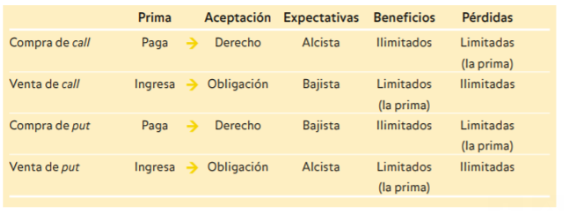
\includegraphics{./images/resumen-opciones.png}

\end{minipage}%
\end{tcolorbox}

\begin{center}\rule{0.5\linewidth}{0.5pt}\end{center}

\begin{enumerate}
\def\labelenumi{\arabic{enumi}.}
\setcounter{enumi}{46}
\tightlist
\item
  Dada la siguiente información, relativa a un contrato de futuros
  IBEX-35
\end{enumerate}

\begin{longtable}[]{@{}l@{}}
\toprule()
\textbf{Datos:} \\
\midrule()
\endhead
Valor Nominal: 150.000 euros \\
Valor Efectivo: 160.000 euros \\
Depósito de garantía: 7.000 euros \\
\bottomrule()
\end{longtable}

¿Qué variación porcentual al alza o a la baja debiera producirse para
``doblar'' o ``perder'' el importe total desembolsado en concepto de
depósito de garantía?:

\begin{enumerate}
\def\labelenumi{\alph{enumi})}
\item
  13,00\%
\item
  4,37\%
\item
  9,00\%
\item
  9,10\%
\end{enumerate}

\begin{tcolorbox}[enhanced jigsaw, colback=white, colframe=quarto-callout-tip-color-frame, rightrule=.15mm, opacityback=0, toprule=.15mm, leftrule=.75mm, arc=.35mm, breakable, bottomrule=.15mm, left=2mm]
\begin{minipage}[t]{5.5mm}
\textcolor{quarto-callout-tip-color}{\faLightbulb}
\end{minipage}%
\begin{minipage}[t]{\textwidth - 5.5mm}

La respuesta \textbf{correcta es la b}.

Para determinar la cifra necesaria para doblar o perder la totalidad del
importe aportado como depósito de garantía, se trata de calcular la
inversa del apalancamiento. Donde el apalncamiento vendrá dado por el
siguuiente cociente:

\[A_{palancamiento}=\frac{Valor\ Efectivo}{Deposito\ Garantia}\]

Y por tanto, la inversa de este, será:

\[\frac {1}{A_{palancamiento}}=\frac {1}{\frac{Valor\ Efectivo}{Deposito\ Garantia}}\]

Ahora bastará con sustituir y calcular en la expresión anterior:

\[\frac {1}{A_{palancamiento}}=\frac {1}{\frac{160.000}{7.000}}=\frac{1}{22,857}=0,04375(4,37\%)\]

Luego la variación porcentual al alza o a la baja debiera producirse
para ``doblar'' o ``perder'' el importe total desembolsado en concepto
de depósito de garantía

\[I_{nversa}=\frac{1}{21.42}=0.0466\]

Si se efectúa la comprobación, \textbf{el lector podrá comprobar que el}
\(4,37\%\) de 160.000 euros son los 7.000 euros del depósito de
garantía.

\end{minipage}%
\end{tcolorbox}

\begin{center}\rule{0.5\linewidth}{0.5pt}\end{center}

\begin{enumerate}
\def\labelenumi{\arabic{enumi}.}
\setcounter{enumi}{47}
\tightlist
\item
  ¿Qué rentabilidad nominal se ha alcanzado en la siguiente operación de
  compra- venta de una opción put llevada hasta la fecha de vencimiento
  y liquidada por diferencias, sin considerar comisiones, ni costes de
  financiación por la prima pagada?:
\end{enumerate}

\begin{longtable}[]{@{}
  >{\raggedright\arraybackslash}p{(\columnwidth - 0\tabcolsep) * \real{1.0000}}@{}}
\toprule()
\begin{minipage}[b]{\linewidth}\raggedright
\textbf{Datos:}
\end{minipage} \\
\midrule()
\endhead
Compra de put ``ATM'' a 20. \\
Precio de ejercicio 200. \\
Revalorización del subyacente (entre compra y liquidación final de la
opción) 30\% \\
\bottomrule()
\end{longtable}

\begin{enumerate}
\def\labelenumi{\alph{enumi})}
\item
  -100\%
\item
  400\%
\item
  200\%
\item
  300\%
\end{enumerate}

\begin{tcolorbox}[enhanced jigsaw, colback=white, colframe=quarto-callout-tip-color-frame, rightrule=.15mm, opacityback=0, toprule=.15mm, leftrule=.75mm, arc=.35mm, breakable, bottomrule=.15mm, left=2mm]
\begin{minipage}[t]{5.5mm}
\textcolor{quarto-callout-tip-color}{\faLightbulb}
\end{minipage}%
\begin{minipage}[t]{\textwidth - 5.5mm}

La respuesta \textbf{correcta es la a}.

Como el subyacente se ha revalorizado un 30\%, significa que en el
vencimiento no debe valer nada. En el inicio de la operación la opción
put estaba ``ATM'', es decir con cotización de subyacente en 200 que
coincidía con el precio de ejercicio, pero si se ha revalorizado el
subyacente y la opción es put, llega a vencimiento ``OTM'', y se ha
perdido la totalidad de la prima pagada, lo que significa una
rentabilidad del 100\% negativo.

\end{minipage}%
\end{tcolorbox}

\begin{center}\rule{0.5\linewidth}{0.5pt}\end{center}

\begin{enumerate}
\def\labelenumi{\arabic{enumi}.}
\setcounter{enumi}{48}
\tightlist
\item
  ¿Qué cifra de beneficio potencial máximo se puede alcanzar con la
  compra de un contrato de futuros sobre índice bursátil?:
\end{enumerate}

\begin{enumerate}
\def\labelenumi{\alph{enumi})}
\item
  El depósito de garantía aportado
\item
  Ilimitado
\item
  El valor nominal del contrato
\item
  Todas las anteriores
\end{enumerate}

\begin{tcolorbox}[enhanced jigsaw, colback=white, colframe=quarto-callout-tip-color-frame, rightrule=.15mm, opacityback=0, toprule=.15mm, leftrule=.75mm, arc=.35mm, breakable, bottomrule=.15mm, left=2mm]
\begin{minipage}[t]{5.5mm}
\textcolor{quarto-callout-tip-color}{\faLightbulb}
\end{minipage}%
\begin{minipage}[t]{\textwidth - 5.5mm}

La respuesta \textbf{correcta es la b}.

El beneficio en un futuro sobre índice bursátil comprado es
potencialmente ilimitado, ya que el precio del subyacente puede subir de
forma ilimitada, o como mínimo no sabemos cual es su límite.

\end{minipage}%
\end{tcolorbox}

\begin{center}\rule{0.5\linewidth}{0.5pt}\end{center}

\begin{enumerate}
\def\labelenumi{\arabic{enumi}.}
\setcounter{enumi}{49}
\tightlist
\item
  En la fecha de vencimiento de una opción call, su valor temporal es:
\end{enumerate}

\begin{enumerate}
\def\labelenumi{\alph{enumi})}
\item
  Positivo.
\item
  Nulo.
\item
  Negativo.
\item
  Ninguno de los anteriores.
\end{enumerate}

\begin{tcolorbox}[enhanced jigsaw, colback=white, colframe=quarto-callout-tip-color-frame, rightrule=.15mm, opacityback=0, toprule=.15mm, leftrule=.75mm, arc=.35mm, breakable, bottomrule=.15mm, left=2mm]
\begin{minipage}[t]{5.5mm}
\textcolor{quarto-callout-tip-color}{\faLightbulb}
\end{minipage}%
\begin{minipage}[t]{\textwidth - 5.5mm}

La respuesta \textbf{correcta es la b}.

Las opciones tienen valor temporal y valor intrínseco, y la suma de
ambas es la prima, pero al llegar al vencimiento el valor de una opción
debe ser igual a su valor intrínseco si está ``ITM'' y cero si está
``ATM'' o ``OTM''. Es decir, en el vencimiento, una opción siempre tiene
valor temporal igual a cero, tanto para Call como para Put.

\end{minipage}%
\end{tcolorbox}

\begin{center}\rule{0.5\linewidth}{0.5pt}\end{center}

\begin{enumerate}
\def\labelenumi{\arabic{enumi}.}
\setcounter{enumi}{50}
\tightlist
\item
  Una opción call strike 10 euros y prima 0,5 euros, si el activo
  subyacente cotiza a 10,3 euros, ¿qué valor temporal tiene?
\end{enumerate}

\begin{enumerate}
\def\labelenumi{\alph{enumi})}
\item
  0,2
\item
  No tiene valor temporal
\item
  0,6
\item
  0,15
\end{enumerate}

\begin{tcolorbox}[enhanced jigsaw, colback=white, colframe=quarto-callout-tip-color-frame, rightrule=.15mm, opacityback=0, toprule=.15mm, leftrule=.75mm, arc=.35mm, breakable, bottomrule=.15mm, left=2mm]
\begin{minipage}[t]{5.5mm}
\textcolor{quarto-callout-tip-color}{\faLightbulb}
\end{minipage}%
\begin{minipage}[t]{\textwidth - 5.5mm}

La respuesta \textbf{correcta es la a}.

El valor de una opción call, su prima, se descompone en valor intrínseco
y valor temporal. El valor intrínseco varía entre 0 y P. Cot-PE. En este
caso, el valor intrínseco es:

\[VI=10.3-10=0.3\] El valor temporal es, por tanto:

\[Prima = VI + VT\] Donde,

\[0.5 = 0.3 + VT\] \[VT= 0.2\]

\end{minipage}%
\end{tcolorbox}

\begin{center}\rule{0.5\linewidth}{0.5pt}\end{center}

52.Un gestor de carteras que administra un fondo de inversión de renta
variable altamente diversificado, cuyo patrimonio está situado hoy en 20
millones de Euros, decide cubrirlo con futuros sobre el IBEX-35.
Determinar el número de contratos según los datos siguientes:

\begin{longtable}[]{@{}l@{}}
\toprule()
\textbf{Datos:} \\
\midrule()
\endhead
Valor nominal de la cartera de renta variable 12.500.000 euros \\
Valor efectivo de la cartera de renta variable 18.000.000 euros \\
IBEX-35 contado 6.408,5 \\
Futuro IBEX-35 vencimiento próximo 6.440,0 \\
Beta global de la cartera (altamente fiable) 1,10 \\
\bottomrule()
\end{longtable}

\begin{enumerate}
\def\labelenumi{\alph{enumi})}
\item
  307
\item
  195
\item
  281
\item
  309
\end{enumerate}

\begin{tcolorbox}[enhanced jigsaw, colback=white, colframe=quarto-callout-tip-color-frame, rightrule=.15mm, opacityback=0, toprule=.15mm, leftrule=.75mm, arc=.35mm, breakable, bottomrule=.15mm, left=2mm]
\begin{minipage}[t]{5.5mm}
\textcolor{quarto-callout-tip-color}{\faLightbulb}
\end{minipage}%
\begin{minipage}[t]{\textwidth - 5.5mm}

La respuesta \textbf{correcta es la d}.

Tenemos que calcular el Ratio de Cobertura (RC) con la siguiente
fórmula:

\[RC=\frac{18000000\cdot1.10}{6408.5\cdot10\cdot(-1)}=-309\]

Al emplear la fórmula el que salga con signo negativo indica que estamos
vendiendo futuros.

\end{minipage}%
\end{tcolorbox}

\begin{center}\rule{0.5\linewidth}{0.5pt}\end{center}

\begin{enumerate}
\def\labelenumi{\arabic{enumi}.}
\setcounter{enumi}{52}
\tightlist
\item
  Un gestor de carteras que administra un fondo de inversión de renta
  variable altamente diversificado, cuyo patrimonio está situado hoy en
  190 millones de Euros, decide cubrirlo con futuros sobre el Ibex-35.
  Determinar el número de contratos según los datos siguientes:
\end{enumerate}

\begin{longtable}[]{@{}l@{}}
\toprule()
\textbf{Datos:} \\
\midrule()
\endhead
Valor nominal de la cartera de renta variable 125.000.000 euros. \\
Valor efectivo de la cartera de renta variable 175.500.000 euros. \\
Ibex-35 contado 8.210,5 \\
Futuro Ibex-35 vencimiento próximo 8.230 \\
Beta global de la cartera (altamente fiable) 1,05 \\
\bottomrule()
\end{longtable}

\begin{enumerate}
\def\labelenumi{\alph{enumi})}
\item
  1599
\item
  2239
\item
  1519
\item
  2244
\end{enumerate}

\begin{tcolorbox}[enhanced jigsaw, colback=white, colframe=quarto-callout-tip-color-frame, rightrule=.15mm, opacityback=0, toprule=.15mm, leftrule=.75mm, arc=.35mm, breakable, bottomrule=.15mm, left=2mm]
\begin{minipage}[t]{5.5mm}
\textcolor{quarto-callout-tip-color}{\faLightbulb}
\end{minipage}%
\begin{minipage}[t]{\textwidth - 5.5mm}

La respuesta \textbf{correcta es la d}.

Tenemos que calcular el Ratio de Cobertura (RC) con la siguiente
fórmula:

\[RC=\frac{175500000\cdot1.05}{8210.5\cdot10\cdot(-1)}=-2224\] Al
emplear la fórmula el que salga con signo negativo indica que estamos
vendiendo futuros.

\end{minipage}%
\end{tcolorbox}

\begin{center}\rule{0.5\linewidth}{0.5pt}\end{center}

\begin{enumerate}
\def\labelenumi{\arabic{enumi}.}
\setcounter{enumi}{53}
\tightlist
\item
  Un inversor tiene perspectivas alcistas y decide operar en el mercado
  de futuros sobre el Ibex 35 comprando el 23/08/2016, 10 contratos de
  futuros con vencimiento diciembre de 2016. El precio de venta es 7.163
  puntos; La cotización actual del índice es 7.358 puntos y el futuro de
  diciembre cotiza a 7.363 puntos (06/09/2016). ¿Cuál habrá sido el
  resultado (pérdida/ganancia) de esta operación?
\end{enumerate}

\begin{enumerate}
\def\labelenumi{\alph{enumi})}
\item
  Ganancia de 20.000 euros.
\item
  Pérdida de 20.000 euros.
\item
  Ganancia de 2.000 euros.
\item
  Ninguna de las anteriores.
\end{enumerate}

\begin{tcolorbox}[enhanced jigsaw, colback=white, colframe=quarto-callout-tip-color-frame, rightrule=.15mm, opacityback=0, toprule=.15mm, leftrule=.75mm, arc=.35mm, breakable, bottomrule=.15mm, left=2mm]
\begin{minipage}[t]{5.5mm}
\textcolor{quarto-callout-tip-color}{\faLightbulb}
\end{minipage}%
\begin{minipage}[t]{\textwidth - 5.5mm}

La respuesta \textbf{correcta es la b}.

Aplicamos la fórmula del beneficio/pérdida para una posición en futuros,

\[B/P=(P_f-P_i)\cdot n^o contratos\cdot multiplicador\] Donde al
sustituir y calcular,

\[B/P=(7163-7363)\cdot 10\cdot 10=-20000\] Es decir, -20.000 euros de
pérdida.

\end{minipage}%
\end{tcolorbox}

\begin{center}\rule{0.5\linewidth}{0.5pt}\end{center}

\begin{enumerate}
\def\labelenumi{\arabic{enumi}.}
\setcounter{enumi}{54}
\tightlist
\item
  ¿Cuál es el grado de apalancamiento de un contrato de futuros cuyo
  valor efectivo es 70.000 euros (nominal 69.800 euros) y por el que nos
  piden un depósito de garantía de 10.000 euros?
\end{enumerate}

\begin{enumerate}
\def\labelenumi{\alph{enumi})}
\item
  7
\item
  70
\item
  10
\item
  6,98
\end{enumerate}

\begin{tcolorbox}[enhanced jigsaw, colback=white, colframe=quarto-callout-tip-color-frame, rightrule=.15mm, opacityback=0, toprule=.15mm, leftrule=.75mm, arc=.35mm, breakable, bottomrule=.15mm, left=2mm]
\begin{minipage}[t]{5.5mm}
\textcolor{quarto-callout-tip-color}{\faLightbulb}
\end{minipage}%
\begin{minipage}[t]{\textwidth - 5.5mm}

La respuesta \textbf{correcta es la a}.

\[A_{palancamiento}=\frac{Efectivo}{Deposito\,garantia}=\frac{70000}{10000}=7\,veces\]

\end{minipage}%
\end{tcolorbox}

\begin{center}\rule{0.5\linewidth}{0.5pt}\end{center}

\begin{enumerate}
\def\labelenumi{\arabic{enumi}.}
\setcounter{enumi}{55}
\tightlist
\item
  ¿Qué rentabilidad nominal se ha alcanzado en la siguiente operación de
  compra de call llevada hasta vencimiento y liquidada por diferencias?:
\end{enumerate}

\begin{longtable}[]{@{}l@{}}
\toprule()
\textbf{Datos:} \\
\midrule()
\endhead
Compra call ATM a 7,5 euros \\
Strike: 150 euros \\
Revalorización del subyacente: + 20\% \\
\bottomrule()
\end{longtable}

\begin{enumerate}
\def\labelenumi{\alph{enumi})}
\item
  -100\%
\item
  -200\%
\item
  -300\%
\item
  -400\%
\end{enumerate}

\begin{tcolorbox}[enhanced jigsaw, colback=white, colframe=quarto-callout-tip-color-frame, rightrule=.15mm, opacityback=0, toprule=.15mm, leftrule=.75mm, arc=.35mm, breakable, bottomrule=.15mm, left=2mm]
\begin{minipage}[t]{5.5mm}
\textcolor{quarto-callout-tip-color}{\faLightbulb}
\end{minipage}%
\begin{minipage}[t]{\textwidth - 5.5mm}

La respuesta \textbf{correcta es la c}.

Subyacente a vencimiento = 150 x (1+0,2) = 180

Diferencias = 180 -- 150 = 30 euros

Rentabilidad = 30 -- 7,5 / 7,5 x 100 = 300\%

En contado la rentabilidad habría sido del 20\%. Aquí podemos ver el
efecto apalancamiento de las opciones. Apalancamiento = 300 / 20 = 15x

Nota: la rentabilidad se calcula como cualquier otra rentabilidad
simple:

\[RS=\frac{Valor\ Final-Valor\ Inicial}{Valor\ Inicial}\cdot100\]

\end{minipage}%
\end{tcolorbox}

\begin{center}\rule{0.5\linewidth}{0.5pt}\end{center}

\begin{enumerate}
\def\labelenumi{\arabic{enumi}.}
\setcounter{enumi}{56}
\tightlist
\item
  ¿Qué porcentaje de participación puede ofrecer el siguiente
  garantizado? Patrimonio inicial del fondo: 130 millones euros.
\end{enumerate}

\begin{itemize}
\item
  Importe destinado a la compra del cupón cero y liquidez: 121 millones
  euros.
\item
  Retribución gestora, depositario y otros gastos: 3 millones.
\item
  Las opciones se compran a 7 euros de prima para un nominal de 91
  euros.
\end{itemize}

\begin{enumerate}
\def\labelenumi{\alph{enumi})}
\item
  -54\%
\item
  -60\%
\item
  -80\%
\item
  -40\%
\end{enumerate}

\begin{tcolorbox}[enhanced jigsaw, colback=white, colframe=quarto-callout-tip-color-frame, rightrule=.15mm, opacityback=0, toprule=.15mm, leftrule=.75mm, arc=.35mm, breakable, bottomrule=.15mm, left=2mm]
\begin{minipage}[t]{5.5mm}
\textcolor{quarto-callout-tip-color}{\faLightbulb}
\end{minipage}%
\begin{minipage}[t]{\textwidth - 5.5mm}

La respuesta \textbf{correcta es la b}.

En los ejercicios pueden darnos directamente la cotización de la opción
o bien darnos la prima y el nominal. En este caso, estamos en la segunda
situación y calculamos la cotización así:

\[C=\frac{P}{N}\] Donde,

\begin{itemize}
\item
  \(C\), es la cotización de la opción. Unidades monetarias que cuesta
  tener una exposición completa a la subida del índice.
\item
  \(P\), es la prima de la opción.
\item
  \(N\), es el nominal del título.
\end{itemize}

Que al calcular nos da un resultado de,

\[C=\frac{7}{91}=0.07692(7.692\%)\]

Ahora calcularemos el porcentaje del efectivo \(\%DO\) captado que
dedicaré a opciones una vez deducida la compra del bono y los gastos del
producto.

\[\%DO=\frac{(130-121-3)}{130}=0.046150(4.615\%)\] Y, finalmente
calculamos \(\%G\) como el porcentaje de la subida que podemos ofrecer:

\[\%G=\frac{\%DO}{\%C}=\frac{0.04615}{0.07692}=0.6(60\%)\]

\end{minipage}%
\end{tcolorbox}

\begin{center}\rule{0.5\linewidth}{0.5pt}\end{center}

\begin{enumerate}
\def\labelenumi{\arabic{enumi}.}
\setcounter{enumi}{57}
\tightlist
\item
  Calcular el precio de un futuro de las acciones de TEF teniendo en
  cuenta los siguientes datos:
\end{enumerate}

\begin{longtable}[]{@{}
  >{\raggedright\arraybackslash}p{(\columnwidth - 0\tabcolsep) * \real{1.0000}}@{}}
\toprule()
\begin{minipage}[b]{\linewidth}\raggedright
\textbf{Datos:}
\end{minipage} \\
\midrule()
\endhead
Vencimiento dentro de 10 meses. \\
Precio del contado: 10 \\
Tipo de interés libre de riesgo: 2,5\% \\
Dividendo: 0,75 euros 2 veces al año (cada 6 meses, el próximo dentro de
3 meses) \\
\bottomrule()
\end{longtable}

\begin{enumerate}
\def\labelenumi{\alph{enumi})}
\item
  9
\item
  9,7
\item
  8,7
\item
  Ninguna de las anteriores.
\end{enumerate}

\begin{tcolorbox}[enhanced jigsaw, colback=white, colframe=quarto-callout-tip-color-frame, rightrule=.15mm, opacityback=0, toprule=.15mm, leftrule=.75mm, arc=.35mm, breakable, bottomrule=.15mm, left=2mm]
\begin{minipage}[t]{5.5mm}
\textcolor{quarto-callout-tip-color}{\faLightbulb}
\end{minipage}%
\begin{minipage}[t]{\textwidth - 5.5mm}

La respuesta \textbf{correcta es la c}.

El precio teórico del futuro es el precio del contado capitalizado a
vencimiento menos los dividendos (también capitalizados a esa fecha) y
se calcula con la siguiente fórmula:

\[F=S\cdot\left((1+i)\cdot\frac{T}{Base}\right)-d\cdot\left((1+i)\cdot\frac{T}{Base}\right)\]
Donde:

\begin{itemize}
\item
  \(F\), es el precio de futuro.
\item
  \(S\), es el precio del contado.
\item
  \(i\), es el tipo de interés libre de riesgo de aquí a vencimiento.
\item
  \(d\), es el dividendo bruto.
\item
  \(T\), es el tiempo hasta vencimiento.
\end{itemize}

Que al sustituir y calcular tenemos,

\[F=10\cdot\left((1+0.025)\cdot\frac{10}{12}\right)-0.75\cdot\left((1+0.025)\cdot\frac{7}{12}\right)-0.75\cdot\left((1+0.025)\cdot\frac{1}{12}\right)=8.7\]

\end{minipage}%
\end{tcolorbox}

\begin{center}\rule{0.5\linewidth}{0.5pt}\end{center}

\begin{enumerate}
\def\labelenumi{\arabic{enumi}.}
\setcounter{enumi}{58}
\tightlist
\item
  Una opción de compra americana sobre un subyacente que no paga
  dividendos:
\end{enumerate}

\begin{enumerate}
\def\labelenumi{\alph{enumi})}
\item
  Siempre cuesta más que una opción de compra europea ya que se puede
  ejercer en cualquier momento hasta vencimiento.
\item
  Cuesta lo mismo que una opción de compra europea ya que no se
  ejercitará antes de vencimiento.
\item
  Cuesta menos que una opción de compra europea.
\item
  Puede costar más o menos que una opción de compra europea según esté
  ``in'' o ``out of the money''.
\end{enumerate}

\begin{tcolorbox}[enhanced jigsaw, colback=white, colframe=quarto-callout-tip-color-frame, rightrule=.15mm, opacityback=0, toprule=.15mm, leftrule=.75mm, arc=.35mm, breakable, bottomrule=.15mm, left=2mm]
\begin{minipage}[t]{5.5mm}
\textcolor{quarto-callout-tip-color}{\faLightbulb}
\end{minipage}%
\begin{minipage}[t]{\textwidth - 5.5mm}

La respuesta \textbf{correcta es la b}.

El reparto de dividendos es uno de los factores que influyen en el
precio de una opción, y que su existencia determina la ambigüedad del
efecto que sobre la prima tiene el plazo a vencimiento, en el caso de
una opción europea.

En ausencia de dividendos las opciones europea y americana tienen el
mismo valor, sin embargo, al tratarse de una opción de compra
\textbf{americana} sobre un \textbf{subyacente que no paga dividendos}
(la opción vale más viva que muerta) \textbf{no se ejercerá}.

\href{https://ddd.uab.cat/pub/ree/02101025v15n2/02101025v15n2p199.pdf}{Más
información pinchando aquí (1)}

\href{https://www.enciclopediafinanciera.com/manual/opciones-americanas.html}{Más
información pinchando aquí (2)}

\href{https://m.riunet.upv.es/bitstream/handle/10251/107084/Cort\%C3\%A9s\%3BBurgos\%3BNavarro\%20-\%20Relaci\%C3\%B3n\%20entre\%20los\%20precios\%20de\%20Opciones\%20Europeas\%20y\%20de\%20Opciones\%20Americanas\%20....pdf?sequence=1\&isAllowed=y}{Más
información pinchando aquí (3)}

\end{minipage}%
\end{tcolorbox}

\begin{center}\rule{0.5\linewidth}{0.5pt}\end{center}

\begin{enumerate}
\def\labelenumi{\arabic{enumi}.}
\setcounter{enumi}{59}
\tightlist
\item
  El vendedor de una opción de venta americana:
\end{enumerate}

\begin{enumerate}
\def\labelenumi{\alph{enumi})}
\item
  Está obligado a vender al precio de ejercicio fijado en cualquier
  fecha hasta el vencimiento.
\item
  Está obligado a vender al precio de ejercicio en la fecha de
  vencimiento.
\item
  Está obligado a comprar al precio de ejercicio en cualquier fecha
  hasta el vencimiento.
\item
  Está obligado a comprar al precio de ejercicio en la fecha de
  vencimiento.
\end{enumerate}

\begin{tcolorbox}[enhanced jigsaw, colback=white, colframe=quarto-callout-tip-color-frame, rightrule=.15mm, opacityback=0, toprule=.15mm, leftrule=.75mm, arc=.35mm, breakable, bottomrule=.15mm, left=2mm]
\begin{minipage}[t]{5.5mm}
\textcolor{quarto-callout-tip-color}{\faLightbulb}
\end{minipage}%
\begin{minipage}[t]{\textwidth - 5.5mm}

La respuesta \textbf{correcta es la c}.

\end{minipage}%
\end{tcolorbox}

\begin{center}\rule{0.5\linewidth}{0.5pt}\end{center}

\begin{enumerate}
\def\labelenumi{\arabic{enumi}.}
\setcounter{enumi}{60}
\tightlist
\item
  Un inversor-especulador decididamente bajista, ¿qué estrategia
  utilizará?:
\end{enumerate}

\begin{enumerate}
\def\labelenumi{\alph{enumi})}
\item
  Venta de futuros
\item
  Compra de futuros
\item
  Compra de Call
\item
  Venta de Put
\end{enumerate}

\begin{tcolorbox}[enhanced jigsaw, colback=white, colframe=quarto-callout-tip-color-frame, rightrule=.15mm, opacityback=0, toprule=.15mm, leftrule=.75mm, arc=.35mm, breakable, bottomrule=.15mm, left=2mm]
\begin{minipage}[t]{5.5mm}
\textcolor{quarto-callout-tip-color}{\faLightbulb}
\end{minipage}%
\begin{minipage}[t]{\textwidth - 5.5mm}

La respuesta \textbf{correcta es la a}.

La compra de futuros y la compra de Call serían estrategias alcistas, y
serían respuestas incorrectas.

La venta de Put supondría un ingreso por cobro de primas con riesgo de
mercado bajista, y por tanto, como el invasor-especulador es
decididamente bajista, sólo sería correcta la venta de futuros.

\end{minipage}%
\end{tcolorbox}

\begin{center}\rule{0.5\linewidth}{0.5pt}\end{center}

\begin{enumerate}
\def\labelenumi{\arabic{enumi}.}
\setcounter{enumi}{61}
\tightlist
\item
  ¿Qué máxima pérdida potencial puede generarse en la venta de
  opciones?:
\end{enumerate}

\begin{enumerate}
\def\labelenumi{\alph{enumi})}
\item
  Ilimitada en Call y Put
\item
  Ilimitada en Call y muy elevada, pero no ilimitada, en Put.
\item
  Ilimitada en Put y muy elevada, pero no ilimitada, en Call.
\item
  Limitada en Call y Put.
\end{enumerate}

\begin{tcolorbox}[enhanced jigsaw, colback=white, colframe=quarto-callout-tip-color-frame, rightrule=.15mm, opacityback=0, toprule=.15mm, leftrule=.75mm, arc=.35mm, breakable, bottomrule=.15mm, left=2mm]
\begin{minipage}[t]{5.5mm}
\textcolor{quarto-callout-tip-color}{\faLightbulb}
\end{minipage}%
\begin{minipage}[t]{\textwidth - 5.5mm}

La respuesta \textbf{correcta es la b}.

La venta de opciones put puede generar pérdidas muy importantes, pero
existe límite, ya que el precio del subyacente como máximo puede ser
igual a cero, y en consecuencia lo máximo que se puede perder es la
diferencia entre el precio de ejercicio más la prima cobrada menos el
precio del subyacente. En las opciones call, la pérdida potencial es
ilimitada, ya que si el subyacente sube indefinidamente, la diferencia
entre cotización de subyacente y precio de ejercicio puede ser
ilimitada.

\end{minipage}%
\end{tcolorbox}

\begin{center}\rule{0.5\linewidth}{0.5pt}\end{center}

\begin{enumerate}
\def\labelenumi{\arabic{enumi}.}
\setcounter{enumi}{62}
\tightlist
\item
  Si el contrato de futuros sobre IBEX-35 cotiza a 14.130 puntos, y se
  exige un depósito en garantía de 9.000 euros: ¿cúal es el factor de
  apalancamiento si se decide operar comprando 2 contratos de futuros
  sobre el IBEX-35). Multiplicador del contrato: 10 euros por punto.
\end{enumerate}

\begin{enumerate}
\def\labelenumi{\alph{enumi})}
\item
  157\%
\item
  1,57 veces.
\item
  31,4 veces.
\item
  15,7 veces.
\end{enumerate}

\begin{tcolorbox}[enhanced jigsaw, colback=white, colframe=quarto-callout-tip-color-frame, rightrule=.15mm, opacityback=0, toprule=.15mm, leftrule=.75mm, arc=.35mm, breakable, bottomrule=.15mm, left=2mm]
\begin{minipage}[t]{5.5mm}
\textcolor{quarto-callout-tip-color}{\faLightbulb}
\end{minipage}%
\begin{minipage}[t]{\textwidth - 5.5mm}

La respuesta \textbf{correcta es la d}.

calcularemos el apalancamiento con la siguiente fórmula,

\[A_{palancamiento}=\frac{Valor\,efectio\cdot multiplicador}{garantia}\]
Donde al sustituir los valores y calcular obtenemos un resultado de,

\[A_{palancamiento}=\frac{14130\cdot10\cdot 2}{9000\cdot2}=15,7\,veces\]

Nota: en el cálculo hemos considerado dos contratos (x2) tanto en el
numerador como en el denominador, no obstante matemáticamente es
indiferente ya que:

\[A_{palancamiento}=\frac{14130\cdot10\cdot 2}{9000\cdot2}=15,7\,veces\]

y,

\[A_{palancamiento}=\frac{14130\cdot10}{9000}=15,7\,veces\]

\end{minipage}%
\end{tcolorbox}

\begin{center}\rule{0.5\linewidth}{0.5pt}\end{center}

\begin{enumerate}
\def\labelenumi{\arabic{enumi}.}
\setcounter{enumi}{63}
\tightlist
\item
  ¿Que porcentaje de participation sobre la revalorizacion total podria
  ofrecer este fondo garantizado?
\end{enumerate}

\begin{itemize}
\item
  Patrimonio inicial del Fondo: 150 millones de euros.
\item
  Importe destinado a la compra de bonos de cupon cero y liquidez para
  garantizar el 100\% del patrimonio initial: 135 millones de euros.
\item
  Importe destinado a retribuir a gestora, depositario, auditoria y
  otros costes e impuestos: 3 millones de euros.
\item
  Las opciones estandar que se compran valen 4 euros de prima por un
  nominal de 40,50 euros.
\end{itemize}

\begin{enumerate}
\def\labelenumi{\alph{enumi})}
\item
  81,00\%
\item
  22,215\%
\item
  60,75\%
\item
  Ninguna de las anteriores
\end{enumerate}

\begin{tcolorbox}[enhanced jigsaw, colback=white, colframe=quarto-callout-tip-color-frame, rightrule=.15mm, opacityback=0, toprule=.15mm, leftrule=.75mm, arc=.35mm, breakable, bottomrule=.15mm, left=2mm]
\begin{minipage}[t]{5.5mm}
\textcolor{quarto-callout-tip-color}{\faLightbulb}
\end{minipage}%
\begin{minipage}[t]{\textwidth - 5.5mm}

\textbf{La respuesta correcta as la a}.

El importer necesario para garantizar el 100\% del patrimonio inicial
(150 millones de euros) es de 138 millones de euros: 135 millones de
euros en concepto de bonos cupon 0 y liquidez, y 3 millones de euros en
concepto de retribution, impuestos, etc.

El imponte necesario para garantizar el 100\% del patrimonio inicial
(150 millones de euros) es de 138 millones de euros: 135 millones de
euros en concepto de bonos cupón O y liquidez, y 3 millones de euros en
concepto de retribución, impuestos, etc.

Por lo tanto, el resto, es decir los 12 millones captados que el fondo
destinará a la búsqueda de rentabilidad, se emplearán para el pago de la
prima de la opción estándar.

Como la prima de dicha opción estándar es de 4 euros para un nominal de
40,50€, el nominal sobre el que el fondo podrá especular con 12 millones
de euros será de:

\[\left(\frac{12\cdot40,50}{4}\right)\cdot100=121,50\]

Un nominal de 121,5 millones de euros, representa sobre el total captado
(150 millones de euros) un porcentaje del:

\[\left(\frac{121,5}{150}\right)\cdot100=81\%\]

Por lo tanto, \textbf{el fondo podrá ofrecer un 81\% de la
revalorización total del subyacente}.

\end{minipage}%
\end{tcolorbox}

\begin{center}\rule{0.5\linewidth}{0.5pt}\end{center}

\begin{enumerate}
\def\labelenumi{\arabic{enumi}.}
\setcounter{enumi}{64}
\tightlist
\item
  El sistema de liquidación de los contratos de futuros se caracteriza
  por:
\end{enumerate}

\begin{enumerate}
\def\labelenumi{\alph{enumi}.}
\item
  Se realiza un pago inmediato en el momento de la compra y de los
  resultados cuando se liquida la operación.
\item
  Se realiza un pago diferido de la compra y también de los resultados
  al vencimiento de la operación.
\item
  No se realiza ningún pago inical y los resultados se liquidan
  diariamente.
\item
  Se realiza un pago inical y los resultados se liquidan diariamente.
\end{enumerate}

\begin{tcolorbox}[enhanced jigsaw, colback=white, colframe=quarto-callout-tip-color-frame, rightrule=.15mm, opacityback=0, toprule=.15mm, leftrule=.75mm, arc=.35mm, breakable, bottomrule=.15mm, left=2mm]
\begin{minipage}[t]{5.5mm}
\textcolor{quarto-callout-tip-color}{\faLightbulb}
\end{minipage}%
\begin{minipage}[t]{\textwidth - 5.5mm}

La respuesta \textbf{correcta es la c}.

\end{minipage}%
\end{tcolorbox}

\begin{center}\rule{0.5\linewidth}{0.5pt}\end{center}

\begin{enumerate}
\def\labelenumi{\arabic{enumi}.}
\setcounter{enumi}{65}
\tightlist
\item
  ¿Cuál de las siguientes afirmaciones sobre el mercado de opciones es
  correcta?
\end{enumerate}

\begin{enumerate}
\def\labelenumi{\alph{enumi}.}
\item
  Si el precio de ejercicio de una CALL es de 10 euros y a vencimiento
  el precio del subyacente es de 10,5 euros, el comprador ejercerá la
  CALL.
\item
  Si el precio de ejercicio de la CALL es 10 euros y la prima de 1 euro,
  el punto muerto de la opción para el comprador es 9 euros.
\item
  Si el precio de ejercicio de la CALL es de 10 euros, la prima pagada
  es de 1 euro y a vencimiento el precio del subyacente es de 10,5
  euros, el comprador de la CALL no la ejercerá.
\item
  El comprador de una CALL de estilo europeo puede ejercer la opción en
  cualquier momento.
\end{enumerate}

\begin{tcolorbox}[enhanced jigsaw, colback=white, colframe=quarto-callout-tip-color-frame, rightrule=.15mm, opacityback=0, toprule=.15mm, leftrule=.75mm, arc=.35mm, breakable, bottomrule=.15mm, left=2mm]
\begin{minipage}[t]{5.5mm}
\textcolor{quarto-callout-tip-color}{\faLightbulb}
\end{minipage}%
\begin{minipage}[t]{\textwidth - 5.5mm}

La respuesta \textbf{correcta es la a}.

Solo con un pequeño matiz, más lingüístico que otra cosa: en realidad el
comprador no necesita ejercer nada, ya que en esta situación a
vencimiento (ITM), el mercado la ejercería automáticamente.

La B no es correcta porque el umbral de rentabilidad o punto muerto para
el comprador de una CALL 10 que ha pagado 1 euros, será 11.

La respuesta C, no es correcta porque el ejercicio o no de la CALL, no
depende de su umbral de rentabilidad, sino de que esté ITM a
vencimiento\ldots y ésta lo está.

La D no es correcta porque las opciones europeas, solo se pueden ejercer
a vencimiento.

Recordemos a las definiciones siguientes:

\begin{itemize}
\item
  \textbf{Opciones Europeas}: Únicamente se pueden ejercer en una fecha
  determinada (fecha de ejercicio). Por ello, tanto el comprador como el
  vendedor deberán esperar a la fecha de vencimiento para determinar si
  la opción se encuentra en dinero o no.
\item
  \textbf{Opciones Americanas}: Pueden ser ejercidas a lo largo de su
  vida en cualquier momento hasta la fecha de ejercicio por aquel que
  tiene el derecho, es decir, el que está comprado.
\end{itemize}

Comprobamos que \textbf{el comprador de una CALL de estilo europeo NO
puede ejercer la opción en cualquier momento}.

\end{minipage}%
\end{tcolorbox}

\begin{center}\rule{0.5\linewidth}{0.5pt}\end{center}

\begin{enumerate}
\def\labelenumi{\arabic{enumi}.}
\setcounter{enumi}{66}
\tightlist
\item
  Si la fluctuación mínima del futuro sobre el Euribor a 3 meses
  negociado en LIFFE (The London International Financial Futures and
  Options Exchange) es de 0,005\% ¿Cuántos ticks de beneficio habrá
  obtenido el comprador de un futuro al 96,000\%, si previamente lo
  había vendido al 97,000\%?
\end{enumerate}

\begin{enumerate}
\def\labelenumi{\alph{enumi})}
\item
  1 tick
\item
  100 ticks
\item
  200 ticks
\item
  1000 ticks
\end{enumerate}

\begin{tcolorbox}[enhanced jigsaw, colback=white, colframe=quarto-callout-tip-color-frame, rightrule=.15mm, opacityback=0, toprule=.15mm, leftrule=.75mm, arc=.35mm, breakable, bottomrule=.15mm, left=2mm]
\begin{minipage}[t]{5.5mm}
\textcolor{quarto-callout-tip-color}{\faLightbulb}
\end{minipage}%
\begin{minipage}[t]{\textwidth - 5.5mm}

La respuesta \textbf{correcta es la c}.

Podemos calcular el beneficio en ticks como:

\[Bº =( 97,000\% - 96,000\% ) \cdot \left(\frac{ 1\ tick}{0,005\%} \right) = 200\]

donde el \textbf{resultado} de la operación será de \textbf{200 ticks}.

\end{minipage}%
\end{tcolorbox}

\begin{center}\rule{0.5\linewidth}{0.5pt}\end{center}

\begin{enumerate}
\def\labelenumi{\arabic{enumi}.}
\setcounter{enumi}{67}
\tightlist
\item
  Con un grado de apalancamiento de 16 veces. ¿Qué variación debe
  experimentar el precio del contrato de futuros que tenemos comprado
  para conseguir un 150\% de rentabilidad absoluta sobre el depósito de
  garantía aportado?
\end{enumerate}

\begin{enumerate}
\def\labelenumi{\alph{enumi})}
\item
  +24\%
\item
  -24\%
\item
  9,375\%
\item
  -9,375\%
\end{enumerate}

\begin{tcolorbox}[enhanced jigsaw, colback=white, colframe=quarto-callout-tip-color-frame, rightrule=.15mm, opacityback=0, toprule=.15mm, leftrule=.75mm, arc=.35mm, breakable, bottomrule=.15mm, left=2mm]
\begin{minipage}[t]{5.5mm}
\textcolor{quarto-callout-tip-color}{\faLightbulb}
\end{minipage}%
\begin{minipage}[t]{\textwidth - 5.5mm}

La respuesta \textbf{correcta es la c}.

La rentabilidad es el resultado de multiplicar el factor de
apalancamiento por la variación del precio,

\[r=A_p\cdot \Delta P\] donde, al \textbf{despejar la variación del
precio} \(\Delta P\) tenemos:

\[\Delta P=\frac{r}{A_p}\] que al sustituir y calcular,

\[\Delta P=\frac {150\% }{16}  = 9,375\%\] tenemos un resutado de
9,375\%. En otras palabras, el precio del contrato de futuros que
tenemos comprado \textbf{deberá experimentar un aumento de precio del
9,375\% para conseguir así un 150\% de rentabilidad absoluta sobre el
depósito de garantía aportado}.

\end{minipage}%
\end{tcolorbox}

\begin{center}\rule{0.5\linewidth}{0.5pt}\end{center}

\begin{enumerate}
\def\labelenumi{\arabic{enumi}.}
\setcounter{enumi}{68}
\tightlist
\item
  Dada la siguiente información, relativa a un contrato de futuros Ibex
  35:
\end{enumerate}

\begin{itemize}
\item
  Valor nominal 87.581 euros
\item
  Valor efectivo 86.830 euros
\item
  Depósito de garantía 12.000 euros
\end{itemize}

¿Qué variación porcentual al alza o a la baja debiera producirse para
doblar o perder el importe total desembolsado en concepto de depósito de
garantía?

\begin{enumerate}
\def\labelenumi{\alph{enumi})}
\item
  14,00\%
\item
  13,82\%
\item
  7,24\%
\item
  14,10\%
\end{enumerate}

\begin{tcolorbox}[enhanced jigsaw, colback=white, colframe=quarto-callout-tip-color-frame, rightrule=.15mm, opacityback=0, toprule=.15mm, leftrule=.75mm, arc=.35mm, breakable, bottomrule=.15mm, left=2mm]
\begin{minipage}[t]{5.5mm}
\textcolor{quarto-callout-tip-color}{\faLightbulb}
\end{minipage}%
\begin{minipage}[t]{\textwidth - 5.5mm}

La respuesta \textbf{correcta es la b}.

Como el factor de apalancamiento es \(7,24\ (86.830 / 12.000)\) y la
variación del precio del futuro que implica doblar o perder el importe
total desembolsado es \(+/-100\%\), tenemos que:

\[\Delta_P =\frac {(+/-\  100\% )}  {7,24 }= 13,82\%\]

\end{minipage}%
\end{tcolorbox}

\begin{center}\rule{0.5\linewidth}{0.5pt}\end{center}

\begin{enumerate}
\def\labelenumi{\arabic{enumi}.}
\setcounter{enumi}{69}
\tightlist
\item
  ¿Qué rentabilidad nominal se ha alcanzado en la siguiente operación de
  compra-venta de una opción call llevada hasta la fecha de vencimiento
  y liquidada por diferencias?
\end{enumerate}

\begin{itemize}
\item
  Compra de call ATM a 15
\item
  Precio de ejercicio 200
\item
  Revalorización del subyacente (entre compra y liquidación final de la
  opción) 30\%
\end{itemize}

\begin{enumerate}
\def\labelenumi{\alph{enumi})}
\item
  100\%
\item
  200\%
\item
  300\%
\item
  400\%
\end{enumerate}

\begin{tcolorbox}[enhanced jigsaw, colback=white, colframe=quarto-callout-tip-color-frame, rightrule=.15mm, opacityback=0, toprule=.15mm, leftrule=.75mm, arc=.35mm, breakable, bottomrule=.15mm, left=2mm]
\begin{minipage}[t]{5.5mm}
\textcolor{quarto-callout-tip-color}{\faLightbulb}
\end{minipage}%
\begin{minipage}[t]{\textwidth - 5.5mm}

La respuesta \textbf{correcta es la c}.

Cuando una opción se encuentra ATM implica que el precio del subyacente
es igual al strike. Por lo tanto:

Precio del subyacente en el momento de la compra, \(P_0= 200\)

Revalorización del subyacente, \(\Delta_P = 30\%\)

Precio del subyacente a vencimiento , \(P_n= 200\cdot (1 + 0,3) = 260\)

Precio de la opción al inicio de la operación \(C_{0}=prima=15\)

Precio de la opción a vencimiento (no hay valor temporal, por lo tanto
la prima será el valor intrínseco de la opción):

\[C_f=200\cdot 30\%=60\]

\[C_0\cdot(1+r)=C_f\]

donde la rentabilidad será,

\[r=\frac{C_f}{C_0}-1\] \[r=\frac{60}{15}-1=3(300\%)\]

\end{minipage}%
\end{tcolorbox}

\begin{center}\rule{0.5\linewidth}{0.5pt}\end{center}

71.Si el contrato de futuros sobre IBEX-35 cotiza a 14.130 puntos, y se
exige un depósito en garantía de 9.000 euros: ¿cúal es el factor de
apalancamiento si se decide operar comprando un contrato de futuros
sobre el IBEX-35). Multiplicador del contrato: 10 euros por punto.

\begin{enumerate}
\def\labelenumi{\alph{enumi})}
\item
  157\%
\item
  1.57 veces.
\item
  31.4 veces.
\item
  15.7 veces.
\end{enumerate}

\begin{tcolorbox}[enhanced jigsaw, colback=white, colframe=quarto-callout-tip-color-frame, rightrule=.15mm, opacityback=0, toprule=.15mm, leftrule=.75mm, arc=.35mm, breakable, bottomrule=.15mm, left=2mm]
\begin{minipage}[t]{5.5mm}
\textcolor{quarto-callout-tip-color}{\faLightbulb}
\end{minipage}%
\begin{minipage}[t]{\textwidth - 5.5mm}

La respuesta \textbf{correcta es la d}.

calcularemos el apalancamiento con la siguiente fórmula,

\[A_{palancamiento}=\frac{Valor\,efectio\cdot multiplicador}{garantia}\]
Donde al sustituir los valores y calcular obtenemos un resultado de,

\[A_{palancamiento}=\frac{14130\cdot10 \cdot 1}{9000}=15.7\,veces\]

\end{minipage}%
\end{tcolorbox}

\begin{center}\rule{0.5\linewidth}{0.5pt}\end{center}

\begin{enumerate}
\def\labelenumi{\arabic{enumi}.}
\setcounter{enumi}{71}
\tightlist
\item
  Dada la siguiente información, relativa a un contrato de futuros
  Ibex-35. ¿Qué variación porcentual al alza o a la baja debiera
  producirse para doblar o perder el importe total desembolsado en
  concepto de depósito de garantía?
\end{enumerate}

\begin{longtable}[]{@{}ll@{}}
\toprule()
Información & \\
\midrule()
\endhead
Valor nominal & 87.581€ \\
Valor efectivo & 86.830€ \\
Depósito garantía & 12.000€ \\
\bottomrule()
\end{longtable}

\begin{enumerate}
\def\labelenumi{\alph{enumi}.}
\item
  Sube, si se trata de una opción call.
\item
  Baja, si se trata de una opción put.
\item
  Sube, si se trata de una opción put.
\item
  Las respuestas a y c son correctas.
\end{enumerate}

\begin{tcolorbox}[enhanced jigsaw, colback=white, colframe=quarto-callout-tip-color-frame, rightrule=.15mm, opacityback=0, toprule=.15mm, leftrule=.75mm, arc=.35mm, breakable, bottomrule=.15mm, left=2mm]
\begin{minipage}[t]{5.5mm}
\textcolor{quarto-callout-tip-color}{\faLightbulb}
\end{minipage}%
\begin{minipage}[t]{\textwidth - 5.5mm}

La respuesta \textbf{correcta es la c}.

\end{minipage}%
\end{tcolorbox}

\begin{center}\rule{0.5\linewidth}{0.5pt}\end{center}

\begin{enumerate}
\def\labelenumi{\arabic{enumi}.}
\setcounter{enumi}{72}
\tightlist
\item
  ¿Qué rentabilidad nominal se ha alcanzado en la siguiente operación de
  compraventa de una opción call llevada hasta la fecha de vencimiento y
  liquidada por diferencias?
\end{enumerate}

\begin{longtable}[]{@{}
  >{\raggedright\arraybackslash}p{(\columnwidth - 0\tabcolsep) * \real{1.0000}}@{}}
\toprule()
\begin{minipage}[b]{\linewidth}\raggedright
Información
\end{minipage} \\
\midrule()
\endhead
Operación CALL ATM a 15 \\
Precio ejercicio 200. \\
Revalorización del subyacente (entre compra y liquidación final de la
opción) 30\%. \\
\bottomrule()
\end{longtable}

\begin{enumerate}
\def\labelenumi{\alph{enumi}.}
\item
  100\%.
\item
  200\%.
\item
  300\%.
\item
  400\%.
\end{enumerate}

\begin{tcolorbox}[enhanced jigsaw, colback=white, colframe=quarto-callout-tip-color-frame, rightrule=.15mm, opacityback=0, toprule=.15mm, leftrule=.75mm, arc=.35mm, breakable, bottomrule=.15mm, left=2mm]
\begin{minipage}[t]{5.5mm}
\textcolor{quarto-callout-tip-color}{\faLightbulb}
\end{minipage}%
\begin{minipage}[t]{\textwidth - 5.5mm}

La respuesta \textbf{correcta es la c}.

\end{minipage}%
\end{tcolorbox}

\begin{center}\rule{0.5\linewidth}{0.5pt}\end{center}

\begin{enumerate}
\def\labelenumi{\arabic{enumi}.}
\setcounter{enumi}{73}
\tightlist
\item
  Una semana antes del vencimiento, un inversor compra por 3 euros una
  opción put con precio de ejercicio de 80 euros, siendo en ese momento
  el valor del subyacente 78 euros. ,Cuál de las siguientes afirmaciones
  es correcta,
\end{enumerate}

\begin{enumerate}
\def\labelenumi{\alph{enumi}.}
\item
  El valor intrínseco de la put es 2 euros
\item
  El valor intrínseco de la put es 1 euro
\item
  El valor intrínseco de la put es 5 euros
\item
  El valor temporal de put es 2 euros
\end{enumerate}

\begin{tcolorbox}[enhanced jigsaw, colback=white, colframe=quarto-callout-tip-color-frame, rightrule=.15mm, opacityback=0, toprule=.15mm, leftrule=.75mm, arc=.35mm, breakable, bottomrule=.15mm, left=2mm]
\begin{minipage}[t]{5.5mm}
\textcolor{quarto-callout-tip-color}{\faLightbulb}
\end{minipage}%
\begin{minipage}[t]{\textwidth - 5.5mm}

La respuesta \textbf{correcta es la:} a.

VI = 80 - 78 = 2 euros

VT = 3 - 2 = 1 euros

\end{minipage}%
\end{tcolorbox}

\begin{center}\rule{0.5\linewidth}{0.5pt}\end{center}

\hypertarget{muxf3dulo-2}{%
\chapter*{Módulo 2}\label{muxf3dulo-2}}
\addcontentsline{toc}{chapter}{Módulo 2}

\markboth{Módulo 2}{Módulo 2}

\hypertarget{fondos-y-sociedades-de-inversiuxf3n-mobiliaria}{%
\section*{Fondos y Sociedades de Inversión
Mobiliaria}\label{fondos-y-sociedades-de-inversiuxf3n-mobiliaria}}
\addcontentsline{toc}{section}{Fondos y Sociedades de Inversión
Mobiliaria}

\markright{Fondos y Sociedades de Inversión Mobiliaria}

\begin{enumerate}
\def\labelenumi{\arabic{enumi}.}
\tightlist
\item
  Señalar alguna de las ventajas de los Fondos de Inversión
\end{enumerate}

\begin{enumerate}
\def\labelenumi{\alph{enumi})}
\item
  Una gestión profesional
\item
  Posibilidad de inversión en prácticamente cualquier mercado
\item
  Supervisión de las inversiones
\item
  Todas las anteriores son correctas
\end{enumerate}

\begin{tcolorbox}[enhanced jigsaw, colback=white, colframe=quarto-callout-tip-color-frame, rightrule=.15mm, opacityback=0, toprule=.15mm, leftrule=.75mm, arc=.35mm, breakable, bottomrule=.15mm, left=2mm]
\begin{minipage}[t]{5.5mm}
\textcolor{quarto-callout-tip-color}{\faLightbulb}
\end{minipage}%
\begin{minipage}[t]{\textwidth - 5.5mm}

La respuesta \textbf{correcta es la d}.

Las tres son ventajas de la inversión en Fondos.

\end{minipage}%
\end{tcolorbox}

\begin{center}\rule{0.5\linewidth}{0.5pt}\end{center}

\begin{enumerate}
\def\labelenumi{\arabic{enumi}.}
\setcounter{enumi}{1}
\tightlist
\item
  A la hora de selecciona entre un universo de inversión es necesario
  tener presente:
\end{enumerate}

\begin{enumerate}
\def\labelenumi{\alph{enumi})}
\item
  El elegido será el de mayor rentabilidad.
\item
  El elegido será el de menor riesgo.
\item
  Lo básico es el prestigio de la Gestora.
\item
  Es necesario homogenizar los Fondos comparados, para posteriormente
  calcular ratios que nos permitan delimitar cual ofrece mejor perfil
  rentabilidad --riesgo.
\end{enumerate}

\begin{tcolorbox}[enhanced jigsaw, colback=white, colframe=quarto-callout-tip-color-frame, rightrule=.15mm, opacityback=0, toprule=.15mm, leftrule=.75mm, arc=.35mm, breakable, bottomrule=.15mm, left=2mm]
\begin{minipage}[t]{5.5mm}
\textcolor{quarto-callout-tip-color}{\faLightbulb}
\end{minipage}%
\begin{minipage}[t]{\textwidth - 5.5mm}

La respuesta \textbf{correcta es la d}.

La comparativa debe hacerse con Fondos homogéneos y con ratios que
combinen la rentabilidad y el riesgo.

\end{minipage}%
\end{tcolorbox}

\begin{center}\rule{0.5\linewidth}{0.5pt}\end{center}

\begin{enumerate}
\def\labelenumi{\arabic{enumi}.}
\setcounter{enumi}{2}
\tightlist
\item
  Atendiendo a las inversiones de las IIC´s, esta pueden ser:
\end{enumerate}

\begin{enumerate}
\def\labelenumi{\alph{enumi})}
\item
  De activos mobiliarios y activos monetarios.
\item
  De activos mobiliarios, activos monetarios Inmobiliarios.
\item
  De carácter financiero y no financiero.
\item
  Ninguna de las anteriores.
\end{enumerate}

\begin{tcolorbox}[enhanced jigsaw, colback=white, colframe=quarto-callout-tip-color-frame, rightrule=.15mm, opacityback=0, toprule=.15mm, leftrule=.75mm, arc=.35mm, breakable, bottomrule=.15mm, left=2mm]
\begin{minipage}[t]{5.5mm}
\textcolor{quarto-callout-tip-color}{\faLightbulb}
\end{minipage}%
\begin{minipage}[t]{\textwidth - 5.5mm}

La respuesta \textbf{correcta es la c}.

En la actualidad las IIC´s se dividen en financieras y no financieras.

\end{minipage}%
\end{tcolorbox}

\begin{center}\rule{0.5\linewidth}{0.5pt}\end{center}

\begin{enumerate}
\def\labelenumi{\arabic{enumi}.}
\setcounter{enumi}{3}
\tightlist
\item
  Los partícipes son:
\end{enumerate}

\begin{enumerate}
\def\labelenumi{\alph{enumi})}
\item
  Personas jurídicas o físicas a las que pertenece la IIC en todas las
  situaciones.
\item
  Persona jurídica o física a la que pertenece la IIC que reviste la
  forma de Fondos de Inversión.
\item
  Persona jurídica o física a la que pertenece la IIC que reviste la
  forma de Sociedad de Inversión.
\item
  Ninguna de las anteriores.
\end{enumerate}

\begin{tcolorbox}[enhanced jigsaw, colback=white, colframe=quarto-callout-tip-color-frame, rightrule=.15mm, opacityback=0, toprule=.15mm, leftrule=.75mm, arc=.35mm, breakable, bottomrule=.15mm, left=2mm]
\begin{minipage}[t]{5.5mm}
\textcolor{quarto-callout-tip-color}{\faLightbulb}
\end{minipage}%
\begin{minipage}[t]{\textwidth - 5.5mm}

La respuesta \textbf{correcta es la b}.

La figura del partícipe se ajusta a la definición de esta respuesta,
puesto que en el caso de la Sociedad de Inversión se trata de
accionistas

\end{minipage}%
\end{tcolorbox}

\begin{center}\rule{0.5\linewidth}{0.5pt}\end{center}

\begin{enumerate}
\def\labelenumi{\arabic{enumi}.}
\setcounter{enumi}{4}
\tightlist
\item
  La aportación de cada inversor a un Fondo de Inversión se documenta a
  través de:
\end{enumerate}

\begin{enumerate}
\def\labelenumi{\alph{enumi})}
\item
  Derechos de propiedad
\item
  Acciones
\item
  Certificados de propiedad
\item
  Ninguna de las anteriores
\end{enumerate}

\begin{tcolorbox}[enhanced jigsaw, colback=white, colframe=quarto-callout-tip-color-frame, rightrule=.15mm, opacityback=0, toprule=.15mm, leftrule=.75mm, arc=.35mm, breakable, bottomrule=.15mm, left=2mm]
\begin{minipage}[t]{5.5mm}
\textcolor{quarto-callout-tip-color}{\faLightbulb}
\end{minipage}%
\begin{minipage}[t]{\textwidth - 5.5mm}

La respuesta \textbf{correcta es la d}.

Puesto que los derechos de propiedad se les denomina participaciones.

\end{minipage}%
\end{tcolorbox}

\begin{center}\rule{0.5\linewidth}{0.5pt}\end{center}

\begin{enumerate}
\def\labelenumi{\arabic{enumi}.}
\setcounter{enumi}{5}
\tightlist
\item
  La principal diferencia entre los Fondos de Inversión y las SICAV es:
\end{enumerate}

\begin{enumerate}
\def\labelenumi{\alph{enumi})}
\item
  El destino de la inversión.
\item
  El órgano de supervisión.
\item
  La Sociedad Gestora y la Depositaria.
\item
  La personalidad jurídica.
\end{enumerate}

\begin{tcolorbox}[enhanced jigsaw, colback=white, colframe=quarto-callout-tip-color-frame, rightrule=.15mm, opacityback=0, toprule=.15mm, leftrule=.75mm, arc=.35mm, breakable, bottomrule=.15mm, left=2mm]
\begin{minipage}[t]{5.5mm}
\textcolor{quarto-callout-tip-color}{\faLightbulb}
\end{minipage}%
\begin{minipage}[t]{\textwidth - 5.5mm}

La respuesta \textbf{correcta es la d}.

La personalidad jurídica de la cual carecen los Fondos de Inversión y no
las SICAV.

\end{minipage}%
\end{tcolorbox}

\begin{center}\rule{0.5\linewidth}{0.5pt}\end{center}

\begin{enumerate}
\def\labelenumi{\arabic{enumi}.}
\setcounter{enumi}{6}
\tightlist
\item
  Los Fondos de Inversión:
\end{enumerate}

\begin{enumerate}
\def\labelenumi{\alph{enumi})}
\item
  Capitalizan los beneficios.
\item
  Reparten los beneficios.
\item
  a y b correctas.
\item
  Ninguna de las anteriores.
\end{enumerate}

\begin{tcolorbox}[enhanced jigsaw, colback=white, colframe=quarto-callout-tip-color-frame, rightrule=.15mm, opacityback=0, toprule=.15mm, leftrule=.75mm, arc=.35mm, breakable, bottomrule=.15mm, left=2mm]
\begin{minipage}[t]{5.5mm}
\textcolor{quarto-callout-tip-color}{\faLightbulb}
\end{minipage}%
\begin{minipage}[t]{\textwidth - 5.5mm}

La respuesta \textbf{correcta es la c}.

Los Fondos se dividen en: de capitalización y de reparto.

\end{minipage}%
\end{tcolorbox}

\begin{center}\rule{0.5\linewidth}{0.5pt}\end{center}

\begin{enumerate}
\def\labelenumi{\arabic{enumi}.}
\setcounter{enumi}{7}
\tightlist
\item
  Los fondos de inversión en la actualidad deben tener al menos:
\end{enumerate}

\begin{enumerate}
\def\labelenumi{\alph{enumi})}
\item
  Siempre 100 partícipes en los FI y 150 en F Monetarios.
\item
  Sea cual sea el fondo 100 partícipes.
\item
  Si es FI 100 y como máximo 20 por compartimento.
\item
  Ninguna de las anteriores.
\end{enumerate}

\begin{tcolorbox}[enhanced jigsaw, colback=white, colframe=quarto-callout-tip-color-frame, rightrule=.15mm, opacityback=0, toprule=.15mm, leftrule=.75mm, arc=.35mm, breakable, bottomrule=.15mm, left=2mm]
\begin{minipage}[t]{5.5mm}
\textcolor{quarto-callout-tip-color}{\faLightbulb}
\end{minipage}%
\begin{minipage}[t]{\textwidth - 5.5mm}

La respuesta \textbf{correcta es la d}.

Ninguna es correcta pues en la actualidad para los Fondos Generales el
número mínimo es de 100, no así para los especiales.

Los Fondos especiales son las Instituciones de Inversión Colectiva libre
Estas instituciones no tienen la obligación de tener 100 pudiendo tener
menor número de partícipes (25). Siendo el número mínimo, que no máximo,
por compartimento de 20.

\end{minipage}%
\end{tcolorbox}

\begin{center}\rule{0.5\linewidth}{0.5pt}\end{center}

\begin{enumerate}
\def\labelenumi{\arabic{enumi}.}
\setcounter{enumi}{8}
\tightlist
\item
  Una Institución de Inversión Colectiva Libre:
\end{enumerate}

\begin{enumerate}
\def\labelenumi{\alph{enumi})}
\item
  Necesita tener como máximo 25 partícipes.
\item
  Necesita tener como mínimo 100 partícipes.
\item
  Necesita como mínimo 25 partícipes.
\item
  Como es libre vale cualquier número de partícipes.
\end{enumerate}

\begin{tcolorbox}[enhanced jigsaw, colback=white, colframe=quarto-callout-tip-color-frame, rightrule=.15mm, opacityback=0, toprule=.15mm, leftrule=.75mm, arc=.35mm, breakable, bottomrule=.15mm, left=2mm]
\begin{minipage}[t]{5.5mm}
\textcolor{quarto-callout-tip-color}{\faLightbulb}
\end{minipage}%
\begin{minipage}[t]{\textwidth - 5.5mm}

La respuesta \textbf{correcta es la c}.

Una Institución de Inversión Colectiva Libre necesita como mínimo 25
partícipes.

\end{minipage}%
\end{tcolorbox}

\begin{center}\rule{0.5\linewidth}{0.5pt}\end{center}

\begin{enumerate}
\def\labelenumi{\arabic{enumi}.}
\setcounter{enumi}{9}
\tightlist
\item
  Definimos a los partícipes de un Fondo de Inversión como:
\end{enumerate}

\begin{enumerate}
\def\labelenumi{\alph{enumi})}
\item
  Los propietarios del Fondo
\item
  La persona física o jurídica que aporta al Fondo
\item
  Persona que ostenta los derechos económicos frente al Fondo
\item
  Todas son correctas
\end{enumerate}

\begin{tcolorbox}[enhanced jigsaw, colback=white, colframe=quarto-callout-tip-color-frame, rightrule=.15mm, opacityback=0, toprule=.15mm, leftrule=.75mm, arc=.35mm, breakable, bottomrule=.15mm, left=2mm]
\begin{minipage}[t]{5.5mm}
\textcolor{quarto-callout-tip-color}{\faLightbulb}
\end{minipage}%
\begin{minipage}[t]{\textwidth - 5.5mm}

La respuesta \textbf{correcta es la d}.

La definición y características de un partícipe coincide con las
respuestas a, b, y c.

\end{minipage}%
\end{tcolorbox}

\begin{center}\rule{0.5\linewidth}{0.5pt}\end{center}

\begin{enumerate}
\def\labelenumi{\arabic{enumi}.}
\setcounter{enumi}{10}
\tightlist
\item
  Dentro de los derechos de los partícipes podríamos señalar:
\end{enumerate}

\begin{enumerate}
\def\labelenumi{\alph{enumi})}
\item
  Participar en la gestión financiera
\item
  Acudir a la Junta General de Partícipes
\item
  Solicitar el traspaso de sus participaciones
\item
  Con la actual legislación la B y la C son correctas
\end{enumerate}

\begin{tcolorbox}[enhanced jigsaw, colback=white, colframe=quarto-callout-tip-color-frame, rightrule=.15mm, opacityback=0, toprule=.15mm, leftrule=.75mm, arc=.35mm, breakable, bottomrule=.15mm, left=2mm]
\begin{minipage}[t]{5.5mm}
\textcolor{quarto-callout-tip-color}{\faLightbulb}
\end{minipage}%
\begin{minipage}[t]{\textwidth - 5.5mm}

La respuesta \textbf{correcta es la c}.

La legislación actual no reconoce la figura de Junta General de
participes ni permite que participen en la gestión financiera.

No existe la figura para los Fondos de Inversión (producto donde el
propietario es el partícipe).

En las IIC´s sólo se reconoce junta general en aquellas que tengan
personalidad jurídica, es decir las SICAV. En concreto junta general de
accionistas (los títulos de propiedad no son participaciones y sus
poseedores partícipes, sino acciones y accionistas respectivamente).

El posible malentendido puede pasar por las IIC´s extranjeras que se
comercializan en España. Las mismas las llamamos Fondos pero realmente
son SICAV y como tales si tienen Junta General de Accionistas.

\end{minipage}%
\end{tcolorbox}

\begin{center}\rule{0.5\linewidth}{0.5pt}\end{center}

\begin{enumerate}
\def\labelenumi{\arabic{enumi}.}
\setcounter{enumi}{11}
\tightlist
\item
  La Sociedad Gestora presenta las siguientes características:
\end{enumerate}

\begin{enumerate}
\def\labelenumi{\alph{enumi})}
\item
  Sociedad Anónima
\item
  Gestiona y administra el Fondo exclusivamente
\item
  Custodia los valores
\item
  Ninguna de las anteriores es correcta
\end{enumerate}

\begin{tcolorbox}[enhanced jigsaw, colback=white, colframe=quarto-callout-tip-color-frame, rightrule=.15mm, opacityback=0, toprule=.15mm, leftrule=.75mm, arc=.35mm, breakable, bottomrule=.15mm, left=2mm]
\begin{minipage}[t]{5.5mm}
\textcolor{quarto-callout-tip-color}{\faLightbulb}
\end{minipage}%
\begin{minipage}[t]{\textwidth - 5.5mm}

La respuesta \textbf{correcta es la a}.

Pues la B no es cierta al gestionar también los traspasos y las
suscripciones de participaciones y claramente la C es tarea de la
entidad custodia.

\end{minipage}%
\end{tcolorbox}

\begin{center}\rule{0.5\linewidth}{0.5pt}\end{center}

\begin{enumerate}
\def\labelenumi{\arabic{enumi}.}
\setcounter{enumi}{12}
\tightlist
\item
  Una sociedad gestora puede:
\end{enumerate}

\begin{enumerate}
\def\labelenumi{\alph{enumi})}
\item
  Gestionar cualquier cartera de inversiones incluida las pertenecientes
  a fondos de pensiones.
\item
  Asesorar en inversiones.
\item
  Gestionar inversiones de capital -- riesgo.
\item
  Todas las anteriores.
\end{enumerate}

\begin{tcolorbox}[enhanced jigsaw, colback=white, colframe=quarto-callout-tip-color-frame, rightrule=.15mm, opacityback=0, toprule=.15mm, leftrule=.75mm, arc=.35mm, breakable, bottomrule=.15mm, left=2mm]
\begin{minipage}[t]{5.5mm}
\textcolor{quarto-callout-tip-color}{\faLightbulb}
\end{minipage}%
\begin{minipage}[t]{\textwidth - 5.5mm}

La respuesta \textbf{correcta es la d}.

Pues puede realizar las labores expuesta en a, b y c.

\end{minipage}%
\end{tcolorbox}

\begin{center}\rule{0.5\linewidth}{0.5pt}\end{center}

\begin{enumerate}
\def\labelenumi{\arabic{enumi}.}
\setcounter{enumi}{13}
\tightlist
\item
  Señalar cual de las siguientes funciones no es necesaria realizarla
  por una Sociedad Gestora:
\end{enumerate}

\begin{enumerate}
\def\labelenumi{\alph{enumi})}
\item
  Calcular el valor de las participaciones.
\item
  Elaborar la información necesaria para distribuir a los partícipes.
\item
  Emitir los certificados de participación.
\item
  Supervisar y controlar a la entidad depositaria.
\end{enumerate}

\begin{tcolorbox}[enhanced jigsaw, colback=white, colframe=quarto-callout-tip-color-frame, rightrule=.15mm, opacityback=0, toprule=.15mm, leftrule=.75mm, arc=.35mm, breakable, bottomrule=.15mm, left=2mm]
\begin{minipage}[t]{5.5mm}
\textcolor{quarto-callout-tip-color}{\faLightbulb}
\end{minipage}%
\begin{minipage}[t]{\textwidth - 5.5mm}

La respuesta \textbf{correcta es la d}.

Dado que al ser entidad de crédito le corresponde al Banco de España o
CNMV dependiendo de los casos.

\end{minipage}%
\end{tcolorbox}

\begin{center}\rule{0.5\linewidth}{0.5pt}\end{center}

\begin{enumerate}
\def\labelenumi{\arabic{enumi}.}
\setcounter{enumi}{14}
\tightlist
\item
  Señalar cual de las siguiente funciones no le corresponde a la Entidad
  Depositaria:
\end{enumerate}

\begin{enumerate}
\def\labelenumi{\alph{enumi})}
\item
  Redactar el reglamento
\item
  Vigilar y supervisar la gestión
\item
  Recibir y custodiar los activos del Fondo
\item
  Elaborar la información necesaria para los partícipes
\end{enumerate}

\begin{tcolorbox}[enhanced jigsaw, colback=white, colframe=quarto-callout-tip-color-frame, rightrule=.15mm, opacityback=0, toprule=.15mm, leftrule=.75mm, arc=.35mm, breakable, bottomrule=.15mm, left=2mm]
\begin{minipage}[t]{5.5mm}
\textcolor{quarto-callout-tip-color}{\faLightbulb}
\end{minipage}%
\begin{minipage}[t]{\textwidth - 5.5mm}

La respuesta \textbf{correcta es la d}.

Dado que el resto son funciones de la entidad depositaria.

\end{minipage}%
\end{tcolorbox}

\begin{center}\rule{0.5\linewidth}{0.5pt}\end{center}

\begin{enumerate}
\def\labelenumi{\arabic{enumi}.}
\setcounter{enumi}{15}
\tightlist
\item
  De acuerdo con la Ley y sobre la pertenencia de Gestora y Depositaria
  al mismo grupo, la Ley marca que:
\end{enumerate}

\begin{enumerate}
\def\labelenumi{\alph{enumi})}
\item
  Pueden pertenecer y de hecho lo son
\item
  No pueden pertenecer
\item
  No tienen que pertenecer y si fuera así sería con procedimiento
  especial
\item
  Ninguna es correcta
\end{enumerate}

\begin{tcolorbox}[enhanced jigsaw, colback=white, colframe=quarto-callout-tip-color-frame, rightrule=.15mm, opacityback=0, toprule=.15mm, leftrule=.75mm, arc=.35mm, breakable, bottomrule=.15mm, left=2mm]
\begin{minipage}[t]{5.5mm}
\textcolor{quarto-callout-tip-color}{\faLightbulb}
\end{minipage}%
\begin{minipage}[t]{\textwidth - 5.5mm}

La respuesta \textbf{correcta es la c}.

Tal y como lo recoge la Ley, la pertenencia de Gestora y Depositaria al
mismo grupo, no está permitida salvo casos con un procedimiento
especial. Esto es así para establecer la denominada ``muralla china''
entre ambas.

\end{minipage}%
\end{tcolorbox}

\begin{center}\rule{0.5\linewidth}{0.5pt}\end{center}

\begin{enumerate}
\def\labelenumi{\arabic{enumi}.}
\setcounter{enumi}{16}
\tightlist
\item
  En caso de Deudas de la Entidad Gestora o Depositaria los Fondos bajo
  su dominio:
\end{enumerate}

\begin{enumerate}
\def\labelenumi{\alph{enumi})}
\item
  Responden con su patrimonio de estas deudas
\item
  No responden nunca con su patrimonio
\item
  Responden en los casos señalados por la Ley
\item
  Solo en casos de blanqueo de dinero de los partícipes
\end{enumerate}

\begin{tcolorbox}[enhanced jigsaw, colback=white, colframe=quarto-callout-tip-color-frame, rightrule=.15mm, opacityback=0, toprule=.15mm, leftrule=.75mm, arc=.35mm, breakable, bottomrule=.15mm, left=2mm]
\begin{minipage}[t]{5.5mm}
\textcolor{quarto-callout-tip-color}{\faLightbulb}
\end{minipage}%
\begin{minipage}[t]{\textwidth - 5.5mm}

La respuesta \textbf{correcta es la b}.

Nunca responden con su patrimonio de las deudas de la entidad Gestora o
Depositaria.

\end{minipage}%
\end{tcolorbox}

\begin{center}\rule{0.5\linewidth}{0.5pt}\end{center}

\begin{enumerate}
\def\labelenumi{\arabic{enumi}.}
\setcounter{enumi}{17}
\tightlist
\item
  En el caso de impago, quiebra, fallo, etc\ldots{} de un activo
  incorporado a la cartera del Fondo:
\end{enumerate}

\begin{enumerate}
\def\labelenumi{\alph{enumi})}
\item
  Responde la Entidad Gestora que es la encargada de la Gestión.
\item
  Responde la Entidad Depositaria que es la encargada de la Custodia.
\item
  Ninguna responde siendo un quebranto para los partícipes.
\item
  Todas las anteriores.
\end{enumerate}

\begin{tcolorbox}[enhanced jigsaw, colback=white, colframe=quarto-callout-tip-color-frame, rightrule=.15mm, opacityback=0, toprule=.15mm, leftrule=.75mm, arc=.35mm, breakable, bottomrule=.15mm, left=2mm]
\begin{minipage}[t]{5.5mm}
\textcolor{quarto-callout-tip-color}{\faLightbulb}
\end{minipage}%
\begin{minipage}[t]{\textwidth - 5.5mm}

La respuesta \textbf{correcta es la c}.

El impago, quiebra, fallo, etc\ldots{} de una inversión en cartera
representa un impacto en la posición de los partícipes.

\end{minipage}%
\end{tcolorbox}

\begin{center}\rule{0.5\linewidth}{0.5pt}\end{center}

\begin{enumerate}
\def\labelenumi{\arabic{enumi}.}
\setcounter{enumi}{18}
\tightlist
\item
  Una participación es:
\end{enumerate}

\begin{enumerate}
\def\labelenumi{\alph{enumi})}
\item
  Parte alícuota en la que se divide el capital de la Gestora.
\item
  El título de propiedad del Fondo.
\item
  Única para cada Fondo.
\item
  Son correctas b y c.
\end{enumerate}

\begin{tcolorbox}[enhanced jigsaw, colback=white, colframe=quarto-callout-tip-color-frame, rightrule=.15mm, opacityback=0, toprule=.15mm, leftrule=.75mm, arc=.35mm, breakable, bottomrule=.15mm, left=2mm]
\begin{minipage}[t]{5.5mm}
\textcolor{quarto-callout-tip-color}{\faLightbulb}
\end{minipage}%
\begin{minipage}[t]{\textwidth - 5.5mm}

La respuesta \textbf{correcta es la b}.

Dado que la actual legislación reconoce la posibilidad de diferentes
tipos de participaciones atendiendo a las comisiones aplicables.

\end{minipage}%
\end{tcolorbox}

\begin{center}\rule{0.5\linewidth}{0.5pt}\end{center}

\begin{enumerate}
\def\labelenumi{\arabic{enumi}.}
\setcounter{enumi}{19}
\tightlist
\item
  La valoración de una participación:
\end{enumerate}

\begin{enumerate}
\def\labelenumi{\alph{enumi})}
\item
  No puede ser diferente para un partícipe de un mismo Fondo
\item
  Es el valor liquidativo
\item
  Se realiza a precios de mercado
\item
  Son correctas la b y la c
\end{enumerate}

\begin{tcolorbox}[enhanced jigsaw, colback=white, colframe=quarto-callout-tip-color-frame, rightrule=.15mm, opacityback=0, toprule=.15mm, leftrule=.75mm, arc=.35mm, breakable, bottomrule=.15mm, left=2mm]
\begin{minipage}[t]{5.5mm}
\textcolor{quarto-callout-tip-color}{\faLightbulb}
\end{minipage}%
\begin{minipage}[t]{\textwidth - 5.5mm}

La respuesta \textbf{correcta es la d}.

Dado que al existir compartimentos dependerá de en que compartimiento
esté el partícipe dentro del Fondo.

\end{minipage}%
\end{tcolorbox}

\begin{center}\rule{0.5\linewidth}{0.5pt}\end{center}

\begin{enumerate}
\def\labelenumi{\arabic{enumi}.}
\setcounter{enumi}{20}
\tightlist
\item
  Referido a la comisión de gestión señalar que aspecto no es cierto:
\end{enumerate}

\begin{enumerate}
\def\labelenumi{\alph{enumi})}
\item
  Es percibido por la Gestora
\item
  Puede ser fija o variable
\item
  Está incluida en el cálculo del valor liquidativo
\item
  Todas son ciertas
\end{enumerate}

\begin{tcolorbox}[enhanced jigsaw, colback=white, colframe=quarto-callout-tip-color-frame, rightrule=.15mm, opacityback=0, toprule=.15mm, leftrule=.75mm, arc=.35mm, breakable, bottomrule=.15mm, left=2mm]
\begin{minipage}[t]{5.5mm}
\textcolor{quarto-callout-tip-color}{\faLightbulb}
\end{minipage}%
\begin{minipage}[t]{\textwidth - 5.5mm}

La respuesta \textbf{correcta es la b}.

Pueden ser fijas, variable y combinadas ambas.

\end{minipage}%
\end{tcolorbox}

\begin{center}\rule{0.5\linewidth}{0.5pt}\end{center}

\begin{enumerate}
\def\labelenumi{\arabic{enumi}.}
\setcounter{enumi}{21}
\tightlist
\item
  Los límites de la comisión de gestión en los FI según el nuevo
  reglamento son:
\end{enumerate}

\begin{enumerate}
\def\labelenumi{\alph{enumi})}
\item
  Un 18\% como mínimo si son sobre resultados
\item
  Un 15\% como máximo si son sobre resultados
\item
  Un 10\% fijo si son sobre resultados
\item
  Ninguna de las anteriores
\end{enumerate}

\begin{tcolorbox}[enhanced jigsaw, colback=white, colframe=quarto-callout-tip-color-frame, rightrule=.15mm, opacityback=0, toprule=.15mm, leftrule=.75mm, arc=.35mm, breakable, bottomrule=.15mm, left=2mm]
\begin{minipage}[t]{5.5mm}
\textcolor{quarto-callout-tip-color}{\faLightbulb}
\end{minipage}%
\begin{minipage}[t]{\textwidth - 5.5mm}

La respuesta \textbf{correcta es la d}.

\end{minipage}%
\end{tcolorbox}

\begin{center}\rule{0.5\linewidth}{0.5pt}\end{center}

\begin{enumerate}
\def\labelenumi{\arabic{enumi}.}
\setcounter{enumi}{22}
\tightlist
\item
  Los límites de la comisión de gestión en los FI según el nuevo
  reglamento son:
\end{enumerate}

\begin{enumerate}
\def\labelenumi{\alph{enumi})}
\item
  Un 2.50\% como mínimo
\item
  Un 2.25\% como máximo
\item
  Un 2.50\% como máximo
\item
  Ninguna de las anteriores
\end{enumerate}

\begin{tcolorbox}[enhanced jigsaw, colback=white, colframe=quarto-callout-tip-color-frame, rightrule=.15mm, opacityback=0, toprule=.15mm, leftrule=.75mm, arc=.35mm, breakable, bottomrule=.15mm, left=2mm]
\begin{minipage}[t]{5.5mm}
\textcolor{quarto-callout-tip-color}{\faLightbulb}
\end{minipage}%
\begin{minipage}[t]{\textwidth - 5.5mm}

La respuesta \textbf{correcta es la b}.

El límite es de 2.25\% como máximo si es sobre patrimonio.

\end{minipage}%
\end{tcolorbox}

\begin{center}\rule{0.5\linewidth}{0.5pt}\end{center}

\begin{enumerate}
\def\labelenumi{\arabic{enumi}.}
\setcounter{enumi}{23}
\tightlist
\item
  Los límites de la comisión mixta de gestión en los FI según el nuevo
  reglamento son:
\end{enumerate}

\begin{enumerate}
\def\labelenumi{\alph{enumi})}
\item
  Un 2.50\% sobre patrimonio y un 18\% sobre resultados
\item
  Un 2.25\% sobre patrimonio y un 18\% sobre resultados
\item
  Un 2.50\% como máximo tanto de patrimonio como resultado
\item
  Un 1.35\% sobre patrimonio y un 9\% sobre resultados
\end{enumerate}

\begin{tcolorbox}[enhanced jigsaw, colback=white, colframe=quarto-callout-tip-color-frame, rightrule=.15mm, opacityback=0, toprule=.15mm, leftrule=.75mm, arc=.35mm, breakable, bottomrule=.15mm, left=2mm]
\begin{minipage}[t]{5.5mm}
\textcolor{quarto-callout-tip-color}{\faLightbulb}
\end{minipage}%
\begin{minipage}[t]{\textwidth - 5.5mm}

La respuesta \textbf{correcta es la d}.

Los límites de la comisión mixta de gestión en los FI según el nuevo
reglamento son un 1.35\% sobre patrimonio y un 9\% sobre resultados.

\end{minipage}%
\end{tcolorbox}

\begin{center}\rule{0.5\linewidth}{0.5pt}\end{center}

\begin{enumerate}
\def\labelenumi{\arabic{enumi}.}
\setcounter{enumi}{24}
\tightlist
\item
  En el caso de las comisiones de gestión de un fondo:
\end{enumerate}

\begin{enumerate}
\def\labelenumi{\alph{enumi})}
\item
  Están incluidas en el cálculo del valor liquidativo
\item
  Son soportadas individualmente por cada partícipes
\item
  Son cobradas por la Gestora
\item
  Todas las anteriores.
\end{enumerate}

\begin{tcolorbox}[enhanced jigsaw, colback=white, colframe=quarto-callout-tip-color-frame, rightrule=.15mm, opacityback=0, toprule=.15mm, leftrule=.75mm, arc=.35mm, breakable, bottomrule=.15mm, left=2mm]
\begin{minipage}[t]{5.5mm}
\textcolor{quarto-callout-tip-color}{\faLightbulb}
\end{minipage}%
\begin{minipage}[t]{\textwidth - 5.5mm}

La respuesta \textbf{correcta es la d}.

Todas son ciertas.

\end{minipage}%
\end{tcolorbox}

\begin{center}\rule{0.5\linewidth}{0.5pt}\end{center}

\begin{enumerate}
\def\labelenumi{\arabic{enumi}.}
\setcounter{enumi}{25}
\tightlist
\item
  La rentabilidad obtenida por un Fondo y que se traslada a un partícipe
  depende de:
\end{enumerate}

\begin{enumerate}
\def\labelenumi{\alph{enumi})}
\item
  La cartera del Fondo.
\item
  La calidad de la Gestión.
\item
  La comisión aplicada a cada Fondo.
\item
  Todas las anteriores.
\end{enumerate}

\begin{tcolorbox}[enhanced jigsaw, colback=white, colframe=quarto-callout-tip-color-frame, rightrule=.15mm, opacityback=0, toprule=.15mm, leftrule=.75mm, arc=.35mm, breakable, bottomrule=.15mm, left=2mm]
\begin{minipage}[t]{5.5mm}
\textcolor{quarto-callout-tip-color}{\faLightbulb}
\end{minipage}%
\begin{minipage}[t]{\textwidth - 5.5mm}

La respuesta \textbf{correcta es la d}.

\end{minipage}%
\end{tcolorbox}

\begin{center}\rule{0.5\linewidth}{0.5pt}\end{center}

\begin{enumerate}
\def\labelenumi{\arabic{enumi}.}
\setcounter{enumi}{26}
\tightlist
\item
  De los siguientes activos señalar en cual no pueden invertir los FI:
\end{enumerate}

\begin{enumerate}
\def\labelenumi{\alph{enumi})}
\item
  Depósitos bancarios
\item
  Títulos que se vayan a admitir a cotización
\item
  Derivados de crédito
\item
  Participaciones de otras IIC
\end{enumerate}

\begin{tcolorbox}[enhanced jigsaw, colback=white, colframe=quarto-callout-tip-color-frame, rightrule=.15mm, opacityback=0, toprule=.15mm, leftrule=.75mm, arc=.35mm, breakable, bottomrule=.15mm, left=2mm]
\begin{minipage}[t]{5.5mm}
\textcolor{quarto-callout-tip-color}{\faLightbulb}
\end{minipage}%
\begin{minipage}[t]{\textwidth - 5.5mm}

La respuesta \textbf{correcta es la c}.

Derivados de crédito ya que el crédito no es un activo financiero.

\end{minipage}%
\end{tcolorbox}

\begin{center}\rule{0.5\linewidth}{0.5pt}\end{center}

\begin{enumerate}
\def\labelenumi{\arabic{enumi}.}
\setcounter{enumi}{27}
\tightlist
\item
  Las participaciones en IIC´s serán activos aptos siempre que:
\end{enumerate}

\begin{enumerate}
\def\labelenumi{\alph{enumi})}
\item
  En todos los casos
\item
  En cualquiera que tenga pasaporte comunitario
\item
  No tengan pasaporte comunitario
\item
  Ninguna de las tres
\end{enumerate}

\begin{tcolorbox}[enhanced jigsaw, colback=white, colframe=quarto-callout-tip-color-frame, rightrule=.15mm, opacityback=0, toprule=.15mm, leftrule=.75mm, arc=.35mm, breakable, bottomrule=.15mm, left=2mm]
\begin{minipage}[t]{5.5mm}
\textcolor{quarto-callout-tip-color}{\faLightbulb}
\end{minipage}%
\begin{minipage}[t]{\textwidth - 5.5mm}

La respuesta \textbf{correcta es la d}.

Puesto que la respuesta B se ve matizada por la necesidad de que esta
instituciones no puedan invertir más de un 10 \% en participaciones de
una única IIC.

\end{minipage}%
\end{tcolorbox}

\begin{center}\rule{0.5\linewidth}{0.5pt}\end{center}

\begin{enumerate}
\def\labelenumi{\arabic{enumi}.}
\setcounter{enumi}{28}
\tightlist
\item
  El límite de diversificación es:
\end{enumerate}

\begin{enumerate}
\def\labelenumi{\alph{enumi})}
\item
  Fijo para todas las IIC´s.
\item
  Una medida de seguridad para los partícipes.
\item
  Es siempre del 10\%.
\item
  Todas son correctas.
\end{enumerate}

\begin{tcolorbox}[enhanced jigsaw, colback=white, colframe=quarto-callout-tip-color-frame, rightrule=.15mm, opacityback=0, toprule=.15mm, leftrule=.75mm, arc=.35mm, breakable, bottomrule=.15mm, left=2mm]
\begin{minipage}[t]{5.5mm}
\textcolor{quarto-callout-tip-color}{\faLightbulb}
\end{minipage}%
\begin{minipage}[t]{\textwidth - 5.5mm}

La respuesta \textbf{correcta es la b}.

Pues el límite es del 5 \% si bien es ampliable al 10 \% cuando la suma
de las posiciones que rebasen el 5 \% no sumen más del 40 \% y en el
caso de los Fondos Índices estos límites pueden verse superados

\end{minipage}%
\end{tcolorbox}

\begin{center}\rule{0.5\linewidth}{0.5pt}\end{center}

\begin{enumerate}
\def\labelenumi{\arabic{enumi}.}
\setcounter{enumi}{29}
\tightlist
\item
  Señalar la incorrecta. El concepto de fondo índice no se ajusta a:
\end{enumerate}

\begin{enumerate}
\def\labelenumi{\alph{enumi})}
\item
  Intentar replicar los resultados de un índice financiero
\item
  Sus límites de diversificación son más amplio que los Fondos normales
\item
  Es una categoría especial de Fondos
\item
  Es un fondo de gestión alternativa
\end{enumerate}

\begin{tcolorbox}[enhanced jigsaw, colback=white, colframe=quarto-callout-tip-color-frame, rightrule=.15mm, opacityback=0, toprule=.15mm, leftrule=.75mm, arc=.35mm, breakable, bottomrule=.15mm, left=2mm]
\begin{minipage}[t]{5.5mm}
\textcolor{quarto-callout-tip-color}{\faLightbulb}
\end{minipage}%
\begin{minipage}[t]{\textwidth - 5.5mm}

La respuesta \textbf{correcta es la d}.

Los fondos índices no son fondos de gestión alternativa.

\end{minipage}%
\end{tcolorbox}

\begin{center}\rule{0.5\linewidth}{0.5pt}\end{center}

\begin{enumerate}
\def\labelenumi{\arabic{enumi}.}
\setcounter{enumi}{30}
\tightlist
\item
  Cuando una persona ha adquirido participaciones y decide reembolsar
  parte de ellas, fiscalmente se identifican las participaciones que
  salen atendiendo al método:
\end{enumerate}

\begin{enumerate}
\def\labelenumi{\alph{enumi})}
\item
  Más beneficios para el partícipe
\item
  Menos beneficioso para el partícipe
\item
  Método FIFO, primera entrada primera salida
\item
  Método LIFO, última entrada primera salida
\end{enumerate}

\begin{tcolorbox}[enhanced jigsaw, colback=white, colframe=quarto-callout-tip-color-frame, rightrule=.15mm, opacityback=0, toprule=.15mm, leftrule=.75mm, arc=.35mm, breakable, bottomrule=.15mm, left=2mm]
\begin{minipage}[t]{5.5mm}
\textcolor{quarto-callout-tip-color}{\faLightbulb}
\end{minipage}%
\begin{minipage}[t]{\textwidth - 5.5mm}

La respuesta \textbf{correcta es la c}.

La ley obliga a la aplicación del FIFO.

\end{minipage}%
\end{tcolorbox}

\begin{center}\rule{0.5\linewidth}{0.5pt}\end{center}

\begin{enumerate}
\def\labelenumi{\arabic{enumi}.}
\setcounter{enumi}{31}
\tightlist
\item
  El traspaso de participaciones está permitido entre:
\end{enumerate}

\begin{enumerate}
\def\labelenumi{\alph{enumi})}
\item
  Fondos de Inversión y SICAV.
\item
  Fondos con Fondos y SICAV con SICAV.
\item
  No está permitido entre compartimentos del mismo Fondo.
\item
  Está permitido solo entre sicavs.
\end{enumerate}

\begin{tcolorbox}[enhanced jigsaw, colback=white, colframe=quarto-callout-tip-color-frame, rightrule=.15mm, opacityback=0, toprule=.15mm, leftrule=.75mm, arc=.35mm, breakable, bottomrule=.15mm, left=2mm]
\begin{minipage}[t]{5.5mm}
\textcolor{quarto-callout-tip-color}{\faLightbulb}
\end{minipage}%
\begin{minipage}[t]{\textwidth - 5.5mm}

La respuesta \textbf{correcta es la a}.

El traspaso de participaciones está permitido entre Fondos de Inversión
y SICAV.

\end{minipage}%
\end{tcolorbox}

\begin{center}\rule{0.5\linewidth}{0.5pt}\end{center}

\begin{enumerate}
\def\labelenumi{\arabic{enumi}.}
\setcounter{enumi}{32}
\tightlist
\item
  La delegación total de la gestión en terceras entidades es una
  característica:
\end{enumerate}

\begin{enumerate}
\def\labelenumi{\alph{enumi})}
\item
  Que no es legal.
\item
  Que pertenece al ordenamiento anterior.
\item
  Que está vigente en el ordenamiento actual.
\item
  No es posible.
\end{enumerate}

\begin{tcolorbox}[enhanced jigsaw, colback=white, colframe=quarto-callout-tip-color-frame, rightrule=.15mm, opacityback=0, toprule=.15mm, leftrule=.75mm, arc=.35mm, breakable, bottomrule=.15mm, left=2mm]
\begin{minipage}[t]{5.5mm}
\textcolor{quarto-callout-tip-color}{\faLightbulb}
\end{minipage}%
\begin{minipage}[t]{\textwidth - 5.5mm}

La respuesta \textbf{correcta es la c}.

Que se contempla en la actualidad dado que anteriormente no se podía
realizar de forma genérica y total.

\end{minipage}%
\end{tcolorbox}

\begin{center}\rule{0.5\linewidth}{0.5pt}\end{center}

\begin{enumerate}
\def\labelenumi{\arabic{enumi}.}
\setcounter{enumi}{33}
\tightlist
\item
  El coeficiente de liquidez:
\end{enumerate}

\begin{enumerate}
\def\labelenumi{\alph{enumi})}
\item
  Garantiza la liquidación de ordenes de compra y venta de activos
\item
  Garantiza la liquidación normal de ordenes de traspasos reembolsos
\item
  Es una medida de política monetaria
\item
  Ninguna de las anteriores es correcta
\end{enumerate}

\begin{tcolorbox}[enhanced jigsaw, colback=white, colframe=quarto-callout-tip-color-frame, rightrule=.15mm, opacityback=0, toprule=.15mm, leftrule=.75mm, arc=.35mm, breakable, bottomrule=.15mm, left=2mm]
\begin{minipage}[t]{5.5mm}
\textcolor{quarto-callout-tip-color}{\faLightbulb}
\end{minipage}%
\begin{minipage}[t]{\textwidth - 5.5mm}

La respuesta \textbf{correcta es la b}.

Se establece para asegurar la liquidación normal de los traspasos y
reembolsos.

\end{minipage}%
\end{tcolorbox}

\begin{center}\rule{0.5\linewidth}{0.5pt}\end{center}

\begin{enumerate}
\def\labelenumi{\arabic{enumi}.}
\setcounter{enumi}{34}
\tightlist
\item
  En los traspasos, el partícipe se dirige a qué entidad, para que
  inicie ésta los procesos necesarios:
\end{enumerate}

\begin{enumerate}
\def\labelenumi{\alph{enumi})}
\item
  A la gestora origen.
\item
  A la gestora destino.
\item
  A la depositaria origen.
\item
  A la depositaria destino.
\end{enumerate}

\begin{tcolorbox}[enhanced jigsaw, colback=white, colframe=quarto-callout-tip-color-frame, rightrule=.15mm, opacityback=0, toprule=.15mm, leftrule=.75mm, arc=.35mm, breakable, bottomrule=.15mm, left=2mm]
\begin{minipage}[t]{5.5mm}
\textcolor{quarto-callout-tip-color}{\faLightbulb}
\end{minipage}%
\begin{minipage}[t]{\textwidth - 5.5mm}

La respuesta \textbf{correcta es la b}.

La encargada de activas los procedimientos para que se cumpla el
traslado es la entidad destino.

\end{minipage}%
\end{tcolorbox}

\begin{center}\rule{0.5\linewidth}{0.5pt}\end{center}

\begin{enumerate}
\def\labelenumi{\arabic{enumi}.}
\setcounter{enumi}{35}
\tightlist
\item
  ¿Cuál de las siguientes afirmaciones es verdadera sobre el partícipe?
\end{enumerate}

\begin{enumerate}
\def\labelenumi{\alph{enumi})}
\item
  Es accionista del Fondo
\item
  Tiene un derecho de propiedad sobre una parte del Fondo.
\item
  Sólo puede obtener el reembolso de sus participaciones con un preaviso
  de 5 días
\item
  Ninguna de las anteriores
\end{enumerate}

\begin{tcolorbox}[enhanced jigsaw, colback=white, colframe=quarto-callout-tip-color-frame, rightrule=.15mm, opacityback=0, toprule=.15mm, leftrule=.75mm, arc=.35mm, breakable, bottomrule=.15mm, left=2mm]
\begin{minipage}[t]{5.5mm}
\textcolor{quarto-callout-tip-color}{\faLightbulb}
\end{minipage}%
\begin{minipage}[t]{\textwidth - 5.5mm}

La respuesta \textbf{correcta es la b}.

El derecho de propiedad del partícipe se documenta a través de las
participaciones, que representan su derecho sobre una parte del Fondo y
sobre las que puede obtener el reembolso en el momento que lo solicite
(salvo que en el folleto se pida un plazo de preaviso por ser un importe
elevado).

\end{minipage}%
\end{tcolorbox}

\begin{center}\rule{0.5\linewidth}{0.5pt}\end{center}

\begin{enumerate}
\def\labelenumi{\arabic{enumi}.}
\setcounter{enumi}{36}
\tightlist
\item
  La Sociedad Gestora
\end{enumerate}

\begin{enumerate}
\def\labelenumi{\alph{enumi})}
\item
  Gestiona siempre la totalidad del Fondo.
\item
  No está obligada a ejercer los derechos económicos del Fondo.
\item
  Es la encargada del cálculo del valor liquidativo.
\item
  No puede gestionar planes de pensiones.
\end{enumerate}

\begin{tcolorbox}[enhanced jigsaw, colback=white, colframe=quarto-callout-tip-color-frame, rightrule=.15mm, opacityback=0, toprule=.15mm, leftrule=.75mm, arc=.35mm, breakable, bottomrule=.15mm, left=2mm]
\begin{minipage}[t]{5.5mm}
\textcolor{quarto-callout-tip-color}{\faLightbulb}
\end{minipage}%
\begin{minipage}[t]{\textwidth - 5.5mm}

La respuesta \textbf{correcta es la c}.

Una de las funciones de la Sociedad Gestora es el cálculo del valor
liquidativo, mientras que puede delegar la gestión de parte o la
totalidad de los activos del Fondo, puede gestionar planes de pensiones
si así lo recoge su objeto social y está obligada a velar por los
derechos del partícipe, de modo que está obligada a ejercer los derechos
económicos del Fondo a favor del partícipe.

\end{minipage}%
\end{tcolorbox}

\begin{center}\rule{0.5\linewidth}{0.5pt}\end{center}

\begin{enumerate}
\def\labelenumi{\arabic{enumi}.}
\setcounter{enumi}{37}
\tightlist
\item
  La Entidad Depositaria:
\end{enumerate}

\begin{enumerate}
\def\labelenumi{\alph{enumi})}
\item
  Deposita y custodia los valores y activos líquidos del Fondo
\item
  Liquida las ordenes de compra y venta de valores que ha ordenado la
  Gestora
\item
  Supervisa la gestión y administración realizada por la Gestora
\item
  Todas las anteriores
\end{enumerate}

\begin{tcolorbox}[enhanced jigsaw, colback=white, colframe=quarto-callout-tip-color-frame, rightrule=.15mm, opacityback=0, toprule=.15mm, leftrule=.75mm, arc=.35mm, breakable, bottomrule=.15mm, left=2mm]
\begin{minipage}[t]{5.5mm}
\textcolor{quarto-callout-tip-color}{\faLightbulb}
\end{minipage}%
\begin{minipage}[t]{\textwidth - 5.5mm}

La respuesta \textbf{correcta es la d}.

Todas ellas son funciones de la Entidad Depositaria.

\end{minipage}%
\end{tcolorbox}

\begin{center}\rule{0.5\linewidth}{0.5pt}\end{center}

\begin{enumerate}
\def\labelenumi{\arabic{enumi}.}
\setcounter{enumi}{38}
\tightlist
\item
  La gestión alternativa se basa en:
\end{enumerate}

\begin{enumerate}
\def\labelenumi{\alph{enumi})}
\item
  Una no correlación de los resultados obtenidos frente al resultados de
  los mercados de inversión
\item
  La obtención, al menos de una rentabilidad objetivo, dentro de unos
  parámetros de volatilidad
\item
  La obtención de una alfa, con una desviación típica determinada
\item
  Todas las anteriores son correctas
\end{enumerate}

\begin{tcolorbox}[enhanced jigsaw, colback=white, colframe=quarto-callout-tip-color-frame, rightrule=.15mm, opacityback=0, toprule=.15mm, leftrule=.75mm, arc=.35mm, breakable, bottomrule=.15mm, left=2mm]
\begin{minipage}[t]{5.5mm}
\textcolor{quarto-callout-tip-color}{\faLightbulb}
\end{minipage}%
\begin{minipage}[t]{\textwidth - 5.5mm}

La respuesta \textbf{correcta es la d}.

Tanto la A, la B y la C son características o definición de gestión
alternativa.

\end{minipage}%
\end{tcolorbox}

\begin{center}\rule{0.5\linewidth}{0.5pt}\end{center}

\begin{enumerate}
\def\labelenumi{\arabic{enumi}.}
\setcounter{enumi}{39}
\tightlist
\item
  La gestión alternativa está justificada por:
\end{enumerate}

\begin{enumerate}
\def\labelenumi{\alph{enumi})}
\item
  Una obtención de resultados siempre positivos
\item
  Un factor de incorrelación de las carteras frente al mercado
\item
  Por ser los tipos de interés muy bajos
\item
  Su alto riesgo sistémico permite aumentar el potencial de rentabilidad
\end{enumerate}

\begin{tcolorbox}[enhanced jigsaw, colback=white, colframe=quarto-callout-tip-color-frame, rightrule=.15mm, opacityback=0, toprule=.15mm, leftrule=.75mm, arc=.35mm, breakable, bottomrule=.15mm, left=2mm]
\begin{minipage}[t]{5.5mm}
\textcolor{quarto-callout-tip-color}{\faLightbulb}
\end{minipage}%
\begin{minipage}[t]{\textwidth - 5.5mm}

La respuesta \textbf{correcta es la b}.

Puesto que el objetivo es la obtención de resultados pero existe riesgo
de pérdida y precisamente el riesgo sistémico no es una característica
de la gestión alternativa.

\end{minipage}%
\end{tcolorbox}

\begin{center}\rule{0.5\linewidth}{0.5pt}\end{center}

\begin{enumerate}
\def\labelenumi{\arabic{enumi}.}
\setcounter{enumi}{40}
\tightlist
\item
  En la gestión alternativa:
\end{enumerate}

\begin{enumerate}
\def\labelenumi{\alph{enumi})}
\item
  El riesgo viene marcado por los activos en los que invierte
\item
  Se sustituye el riesgo de mercado, sistémico, por el de gestión
\item
  Se busca exclusivamente tasas de rentabilidad absolutas lo más latas
  posibles
\item
  No existe definición de riesgo
\end{enumerate}

\begin{tcolorbox}[enhanced jigsaw, colback=white, colframe=quarto-callout-tip-color-frame, rightrule=.15mm, opacityback=0, toprule=.15mm, leftrule=.75mm, arc=.35mm, breakable, bottomrule=.15mm, left=2mm]
\begin{minipage}[t]{5.5mm}
\textcolor{quarto-callout-tip-color}{\faLightbulb}
\end{minipage}%
\begin{minipage}[t]{\textwidth - 5.5mm}

La respuesta \textbf{correcta es la b}.

En la gestión alternativa el gestor tiene libertad de inversión, la
disciplina viene marcada por existir un riesgo determinado (volatilidad)
y a diferencia de los hedged fund no busca maximizar la rentabilidad.

\end{minipage}%
\end{tcolorbox}

\begin{center}\rule{0.5\linewidth}{0.5pt}\end{center}

\begin{enumerate}
\def\labelenumi{\arabic{enumi}.}
\setcounter{enumi}{41}
\tightlist
\item
  Los Hedge Fund o Institución de Inversión Colectiva libre:
\end{enumerate}

\begin{enumerate}
\def\labelenumi{\alph{enumi})}
\item
  Buscan maximizar la rentabilidad por encima de cualquier concepto
\item
  No tiene definido grado de riesgo
\item
  Gestionan, para obtener beneficio, tanto al alza como a la baja en los
  mercados financieros
\item
  Todas las anteriores
\end{enumerate}

\begin{tcolorbox}[enhanced jigsaw, colback=white, colframe=quarto-callout-tip-color-frame, rightrule=.15mm, opacityback=0, toprule=.15mm, leftrule=.75mm, arc=.35mm, breakable, bottomrule=.15mm, left=2mm]
\begin{minipage}[t]{5.5mm}
\textcolor{quarto-callout-tip-color}{\faLightbulb}
\end{minipage}%
\begin{minipage}[t]{\textwidth - 5.5mm}

La respuesta \textbf{correcta es la d}.

Ya que a, b y c son características de la gestión de hedge fund.

\end{minipage}%
\end{tcolorbox}

\begin{center}\rule{0.5\linewidth}{0.5pt}\end{center}

\begin{enumerate}
\def\labelenumi{\arabic{enumi}.}
\setcounter{enumi}{42}
\tightlist
\item
  Cual de las siguientes afirmaciones no es cierta:
\end{enumerate}

\begin{enumerate}
\def\labelenumi{\alph{enumi})}
\item
  Los niveles de apalancamiento de los Hedge Fund suelen ser muy
  considerables.
\item
  En la gestión tradicional el riesgo fundamental del partícipe es el
  sistémico.
\item
  La gestión alternativa busca principalmente la creación del valor
  (alfa).
\item
  Ninguna de las tres.
\end{enumerate}

\begin{tcolorbox}[enhanced jigsaw, colback=white, colframe=quarto-callout-tip-color-frame, rightrule=.15mm, opacityback=0, toprule=.15mm, leftrule=.75mm, arc=.35mm, breakable, bottomrule=.15mm, left=2mm]
\begin{minipage}[t]{5.5mm}
\textcolor{quarto-callout-tip-color}{\faLightbulb}
\end{minipage}%
\begin{minipage}[t]{\textwidth - 5.5mm}

La respuesta \textbf{correcta es la c}.

Puesto que busca la maximización del binomio rentabilidad riesgo.

\end{minipage}%
\end{tcolorbox}

\begin{center}\rule{0.5\linewidth}{0.5pt}\end{center}

\begin{enumerate}
\def\labelenumi{\arabic{enumi}.}
\setcounter{enumi}{43}
\tightlist
\item
  La característica fundamental de los Fondos denominados Neutral Market
  Fund es:
\end{enumerate}

\begin{enumerate}
\def\labelenumi{\alph{enumi})}
\item
  Buscar movimientos direccionales.
\item
  No exponerse a los posibles movimientos de mercado.
\item
  Toman sus decisiones basándose en decisiones sistemáticas.
\item
  Son correctas la a y la b.
\end{enumerate}

\begin{tcolorbox}[enhanced jigsaw, colback=white, colframe=quarto-callout-tip-color-frame, rightrule=.15mm, opacityback=0, toprule=.15mm, leftrule=.75mm, arc=.35mm, breakable, bottomrule=.15mm, left=2mm]
\begin{minipage}[t]{5.5mm}
\textcolor{quarto-callout-tip-color}{\faLightbulb}
\end{minipage}%
\begin{minipage}[t]{\textwidth - 5.5mm}

La respuesta \textbf{correcta es la b}.

Intentan no exponerse al mercado si bien pueden tomar decisiones
sistemáticas o discrecionales.

\end{minipage}%
\end{tcolorbox}

\begin{center}\rule{0.5\linewidth}{0.5pt}\end{center}

\begin{enumerate}
\def\labelenumi{\arabic{enumi}.}
\setcounter{enumi}{44}
\tightlist
\item
  Un fondo de situaciones especiales es:
\end{enumerate}

\begin{enumerate}
\def\labelenumi{\alph{enumi})}
\item
  Búsqueda de valores afectados por alguna característica que influye en
  la formación del precio.
\item
  Buscan situaciones especiales que permitan el arbitraje.
\item
  Invierten en convertible.
\item
  Ninguna de las anteriores.
\end{enumerate}

\begin{tcolorbox}[enhanced jigsaw, colback=white, colframe=quarto-callout-tip-color-frame, rightrule=.15mm, opacityback=0, toprule=.15mm, leftrule=.75mm, arc=.35mm, breakable, bottomrule=.15mm, left=2mm]
\begin{minipage}[t]{5.5mm}
\textcolor{quarto-callout-tip-color}{\faLightbulb}
\end{minipage}%
\begin{minipage}[t]{\textwidth - 5.5mm}

La respuesta \textbf{correcta es la a}.

Invierte en valores que ven su precio presionado por alguna
característica: privatizaciones, ampliaciones, convergencias,
colocaciones, etc.

\end{minipage}%
\end{tcolorbox}

\begin{center}\rule{0.5\linewidth}{0.5pt}\end{center}

\begin{enumerate}
\def\labelenumi{\arabic{enumi}.}
\setcounter{enumi}{45}
\tightlist
\item
  Un fondo Long -- short:
\end{enumerate}

\begin{enumerate}
\def\labelenumi{\alph{enumi})}
\item
  Toma posiciones largas cuando el mercado va a subir y viceversa
\item
  Suele buscar una horquilla de valores e invierte largo o corto en
  ambos en función de las expectativas
\item
  Invierte en una horquilla de valores los cuales deberán tender a
  converger, en el barato compran y en el caro venden
\item
  Realizan arbitrajes de divisas
\end{enumerate}

\begin{tcolorbox}[enhanced jigsaw, colback=white, colframe=quarto-callout-tip-color-frame, rightrule=.15mm, opacityback=0, toprule=.15mm, leftrule=.75mm, arc=.35mm, breakable, bottomrule=.15mm, left=2mm]
\begin{minipage}[t]{5.5mm}
\textcolor{quarto-callout-tip-color}{\faLightbulb}
\end{minipage}%
\begin{minipage}[t]{\textwidth - 5.5mm}

La respuesta \textbf{correcta es la c}.

Es la característica de inversión de estos fondos.

\end{minipage}%
\end{tcolorbox}

\begin{center}\rule{0.5\linewidth}{0.5pt}\end{center}

\begin{enumerate}
\def\labelenumi{\arabic{enumi}.}
\setcounter{enumi}{46}
\tightlist
\item
  Un fondo de arbitraje es:
\end{enumerate}

\begin{enumerate}
\def\labelenumi{\alph{enumi})}
\item
  Toma posiciones en activos cuyo precio no está bien formado y
  necesariamente el mercado corregirá esta situación
\item
  Generalmente se realiza a través de inversiones en divisa y tipos de
  interés
\item
  Puede invertir en convertibles
\item
  Todas las anteriores
\end{enumerate}

\begin{tcolorbox}[enhanced jigsaw, colback=white, colframe=quarto-callout-tip-color-frame, rightrule=.15mm, opacityback=0, toprule=.15mm, leftrule=.75mm, arc=.35mm, breakable, bottomrule=.15mm, left=2mm]
\begin{minipage}[t]{5.5mm}
\textcolor{quarto-callout-tip-color}{\faLightbulb}
\end{minipage}%
\begin{minipage}[t]{\textwidth - 5.5mm}

La respuesta \textbf{correcta es la d}.

Ya que en a, b y c se define lo que es un fondo de arbitraje.

\end{minipage}%
\end{tcolorbox}

\begin{center}\rule{0.5\linewidth}{0.5pt}\end{center}

\begin{enumerate}
\def\labelenumi{\arabic{enumi}.}
\setcounter{enumi}{47}
\tightlist
\item
  La gestión alternativa es una forma:
\end{enumerate}

\begin{enumerate}
\def\labelenumi{\alph{enumi})}
\item
  De diversificación.
\item
  De tener siempre rendimientos positivos.
\item
  De tener herramienta básica a la hora de constituir un patrimonio.
\item
  De pagar muchas comisiones.
\end{enumerate}

\begin{tcolorbox}[enhanced jigsaw, colback=white, colframe=quarto-callout-tip-color-frame, rightrule=.15mm, opacityback=0, toprule=.15mm, leftrule=.75mm, arc=.35mm, breakable, bottomrule=.15mm, left=2mm]
\begin{minipage}[t]{5.5mm}
\textcolor{quarto-callout-tip-color}{\faLightbulb}
\end{minipage}%
\begin{minipage}[t]{\textwidth - 5.5mm}

La respuesta \textbf{correcta es la a}.

La gestión alternativa se debe considerar como diversificadora.

\end{minipage}%
\end{tcolorbox}

\begin{center}\rule{0.5\linewidth}{0.5pt}\end{center}

\begin{enumerate}
\def\labelenumi{\arabic{enumi}.}
\setcounter{enumi}{48}
\tightlist
\item
  Hedge - Fund son:
\end{enumerate}

\begin{enumerate}
\def\labelenumi{\alph{enumi})}
\item
  Fondos de muy bajo riesgo al no presentar correlación con los
  mercados.
\item
  Fondos con betas cercanas a 1.
\item
  Fondos para cubrir (hedged) otros riesgos.
\item
  Ninguna de las anteriores.
\end{enumerate}

\begin{tcolorbox}[enhanced jigsaw, colback=white, colframe=quarto-callout-tip-color-frame, rightrule=.15mm, opacityback=0, toprule=.15mm, leftrule=.75mm, arc=.35mm, breakable, bottomrule=.15mm, left=2mm]
\begin{minipage}[t]{5.5mm}
\textcolor{quarto-callout-tip-color}{\faLightbulb}
\end{minipage}%
\begin{minipage}[t]{\textwidth - 5.5mm}

La respuesta \textbf{correcta es la d}.

Dado que la gestión de un Hedge - Fund no se caracteriza por ninguna de
las tres respuestas (a,b y c).

\end{minipage}%
\end{tcolorbox}

\begin{center}\rule{0.5\linewidth}{0.5pt}\end{center}

\begin{enumerate}
\def\labelenumi{\arabic{enumi}.}
\setcounter{enumi}{49}
\tightlist
\item
  La gestión Alternativa busca:
\end{enumerate}

\begin{enumerate}
\def\labelenumi{\alph{enumi})}
\item
  Maximizar la Beta
\item
  Apalancarse en el mercado
\item
  Reducir la volatilidad de los retornos y maximizar el Alpha
\item
  Asumir más riesgo para obtener una mayor rentabilidad
\end{enumerate}

\begin{tcolorbox}[enhanced jigsaw, colback=white, colframe=quarto-callout-tip-color-frame, rightrule=.15mm, opacityback=0, toprule=.15mm, leftrule=.75mm, arc=.35mm, breakable, bottomrule=.15mm, left=2mm]
\begin{minipage}[t]{5.5mm}
\textcolor{quarto-callout-tip-color}{\faLightbulb}
\end{minipage}%
\begin{minipage}[t]{\textwidth - 5.5mm}

La respuesta \textbf{correcta es la c}.

Ya que el objetivo que busca la gestión Alternativa es maximizar la
rentabilidad minimizando el riesgo.

\end{minipage}%
\end{tcolorbox}

\begin{center}\rule{0.5\linewidth}{0.5pt}\end{center}

\begin{enumerate}
\def\labelenumi{\arabic{enumi}.}
\setcounter{enumi}{50}
\tightlist
\item
  Las estrategias de ``Market Neutral''
\end{enumerate}

\begin{enumerate}
\def\labelenumi{\alph{enumi})}
\item
  No están invertidas en mercado porque son neutrales
\item
  Buscan tener una Beta = 0
\item
  Ganan cuando el mercado sube
\item
  Son muy volátiles
\end{enumerate}

\begin{tcolorbox}[enhanced jigsaw, colback=white, colframe=quarto-callout-tip-color-frame, rightrule=.15mm, opacityback=0, toprule=.15mm, leftrule=.75mm, arc=.35mm, breakable, bottomrule=.15mm, left=2mm]
\begin{minipage}[t]{5.5mm}
\textcolor{quarto-callout-tip-color}{\faLightbulb}
\end{minipage}%
\begin{minipage}[t]{\textwidth - 5.5mm}

La respuesta \textbf{correcta es la b}.

Al renunciar al riesgo sistémico la beta de la cartera es 0.

\end{minipage}%
\end{tcolorbox}

\begin{center}\rule{0.5\linewidth}{0.5pt}\end{center}

\begin{enumerate}
\def\labelenumi{\arabic{enumi}.}
\setcounter{enumi}{51}
\tightlist
\item
  La correlación de la gestión alternativa con las inversiones
  tradicionales:
\end{enumerate}

\begin{enumerate}
\def\labelenumi{\alph{enumi})}
\item
  Sube cuando el mercado cae.
\item
  Cae cuando el mercado sube.
\item
  Busca ser mínima en todas las situaciones de mercado.
\item
  Es enorme, ya que la gestión alternativa utiliza instrumentos de los
  mercados tradicionales.
\end{enumerate}

\begin{tcolorbox}[enhanced jigsaw, colback=white, colframe=quarto-callout-tip-color-frame, rightrule=.15mm, opacityback=0, toprule=.15mm, leftrule=.75mm, arc=.35mm, breakable, bottomrule=.15mm, left=2mm]
\begin{minipage}[t]{5.5mm}
\textcolor{quarto-callout-tip-color}{\faLightbulb}
\end{minipage}%
\begin{minipage}[t]{\textwidth - 5.5mm}

La respuesta \textbf{correcta es la c}.

Busca precisamente la descorrelación con la evolución de los mercados.

\end{minipage}%
\end{tcolorbox}

\begin{center}\rule{0.5\linewidth}{0.5pt}\end{center}

\begin{enumerate}
\def\labelenumi{\arabic{enumi}.}
\setcounter{enumi}{52}
\tightlist
\item
  La fondos de gestión alternativa los podemos dividir en:
\end{enumerate}

\begin{enumerate}
\def\labelenumi{\alph{enumi})}
\item
  Renta fija, renta variable.
\item
  De alta o baja volatilidad.
\item
  Direccionales o no direccionales.
\item
  FI y FIM.
\end{enumerate}

\begin{tcolorbox}[enhanced jigsaw, colback=white, colframe=quarto-callout-tip-color-frame, rightrule=.15mm, opacityback=0, toprule=.15mm, leftrule=.75mm, arc=.35mm, breakable, bottomrule=.15mm, left=2mm]
\begin{minipage}[t]{5.5mm}
\textcolor{quarto-callout-tip-color}{\faLightbulb}
\end{minipage}%
\begin{minipage}[t]{\textwidth - 5.5mm}

La respuesta \textbf{correcta es la c}.

Que da la característica de inversión en las diferentes estrategias.

\end{minipage}%
\end{tcolorbox}

\begin{center}\rule{0.5\linewidth}{0.5pt}\end{center}

\begin{enumerate}
\def\labelenumi{\arabic{enumi}.}
\setcounter{enumi}{53}
\tightlist
\item
  El comportamiento de los fondos de Gestión alternativa se mide por:
\end{enumerate}

\begin{enumerate}
\def\labelenumi{\alph{enumi})}
\item
  Ratio Sharpe.
\item
  Comparación con respecto a su Benchmark.
\item
  No se miden porque no hay datos.
\item
  Duración.
\end{enumerate}

\begin{tcolorbox}[enhanced jigsaw, colback=white, colframe=quarto-callout-tip-color-frame, rightrule=.15mm, opacityback=0, toprule=.15mm, leftrule=.75mm, arc=.35mm, breakable, bottomrule=.15mm, left=2mm]
\begin{minipage}[t]{5.5mm}
\textcolor{quarto-callout-tip-color}{\faLightbulb}
\end{minipage}%
\begin{minipage}[t]{\textwidth - 5.5mm}

La respuesta \textbf{correcta es la a}.

\end{minipage}%
\end{tcolorbox}

\begin{center}\rule{0.5\linewidth}{0.5pt}\end{center}

\begin{enumerate}
\def\labelenumi{\arabic{enumi}.}
\setcounter{enumi}{54}
\tightlist
\item
  Los fondos de Gestión Alternativa domiciliados en España:
\end{enumerate}

\begin{enumerate}
\def\labelenumi{\alph{enumi})}
\item
  Tienen que estar registrados en la CNMV.
\item
  Venden en corto para ganar cuando el mercado baja.
\item
  Son fondos garantizados.
\item
  No existen fondos de gestión alternativa en España.
\end{enumerate}

\begin{tcolorbox}[enhanced jigsaw, colback=white, colframe=quarto-callout-tip-color-frame, rightrule=.15mm, opacityback=0, toprule=.15mm, leftrule=.75mm, arc=.35mm, breakable, bottomrule=.15mm, left=2mm]
\begin{minipage}[t]{5.5mm}
\textcolor{quarto-callout-tip-color}{\faLightbulb}
\end{minipage}%
\begin{minipage}[t]{\textwidth - 5.5mm}

La respuesta \textbf{correcta es la a}.

\end{minipage}%
\end{tcolorbox}

\begin{center}\rule{0.5\linewidth}{0.5pt}\end{center}

\begin{enumerate}
\def\labelenumi{\arabic{enumi}.}
\setcounter{enumi}{55}
\tightlist
\item
  La diferencia principal entre un FI de Renta Fija y un Fondo Monetario
  consiste en:
\end{enumerate}

\begin{enumerate}
\def\labelenumi{\alph{enumi}.}
\item
  La liquidez mínima exigida.
\item
  Las limitaciones en las Inversiones.
\item
  El tipo de Gestora que requieren
\item
  El número de participaciones puestas inicialmente en circulación.
\end{enumerate}

\begin{tcolorbox}[enhanced jigsaw, colback=white, colframe=quarto-callout-tip-color-frame, rightrule=.15mm, opacityback=0, toprule=.15mm, leftrule=.75mm, arc=.35mm, breakable, bottomrule=.15mm, left=2mm]
\begin{minipage}[t]{5.5mm}
\textcolor{quarto-callout-tip-color}{\faLightbulb}
\end{minipage}%
\begin{minipage}[t]{\textwidth - 5.5mm}

La \textbf{respuesta correcta es la b}.

\end{minipage}%
\end{tcolorbox}

\begin{center}\rule{0.5\linewidth}{0.5pt}\end{center}

\begin{enumerate}
\def\labelenumi{\arabic{enumi}.}
\setcounter{enumi}{56}
\tightlist
\item
  ¿Qué le ocurrirá a un FI de renta fija a largo plazo si suben los
  tipos de interés a largo plazo?
\end{enumerate}

\begin{enumerate}
\def\labelenumi{\alph{enumi}.}
\item
  Nada, pues no van a comprar activos hasta que vuelvan a bajar los
  tipos de interés.
\item
  Subirá el valor de las Participaciones.
\item
  Bajará el valor de las Participaciones.
\item
  Dependerá de cómo pueda renovar a vencimiento los activos.
\end{enumerate}

\begin{tcolorbox}[enhanced jigsaw, colback=white, colframe=quarto-callout-tip-color-frame, rightrule=.15mm, opacityback=0, toprule=.15mm, leftrule=.75mm, arc=.35mm, breakable, bottomrule=.15mm, left=2mm]
\begin{minipage}[t]{5.5mm}
\textcolor{quarto-callout-tip-color}{\faLightbulb}
\end{minipage}%
\begin{minipage}[t]{\textwidth - 5.5mm}

La \textbf{respuesta correcta es la c}.

\end{minipage}%
\end{tcolorbox}

\begin{center}\rule{0.5\linewidth}{0.5pt}\end{center}

\begin{enumerate}
\def\labelenumi{\arabic{enumi}.}
\setcounter{enumi}{57}
\tightlist
\item
  ¿Cuál es el plazo máximo de reembolso de un FI?
\end{enumerate}

\begin{enumerate}
\def\labelenumi{\alph{enumi}.}
\item
  1 mes.
\item
  10 días hábiles.
\item
  3 días.
\item
  24 horas, salvo situaciones previstas reglamentariamente.
\end{enumerate}

\begin{tcolorbox}[enhanced jigsaw, colback=white, colframe=quarto-callout-tip-color-frame, rightrule=.15mm, opacityback=0, toprule=.15mm, leftrule=.75mm, arc=.35mm, breakable, bottomrule=.15mm, left=2mm]
\begin{minipage}[t]{5.5mm}
\textcolor{quarto-callout-tip-color}{\faLightbulb}
\end{minipage}%
\begin{minipage}[t]{\textwidth - 5.5mm}

La \textbf{respuesta correcta es la c}.

\end{minipage}%
\end{tcolorbox}

\begin{center}\rule{0.5\linewidth}{0.5pt}\end{center}

\begin{enumerate}
\def\labelenumi{\arabic{enumi}.}
\setcounter{enumi}{58}
\tightlist
\item
  Un fondo de inversión que tiene la siguiente estructura de cartera:
\end{enumerate}

\begin{itemize}
\item
  Acciones europeas (euros) 2 \%
\item
  Acciones nacionales (euros) 88 \%
\item
  Acciones europeas no euro (libras) 5 \%
\item
  Activos monetarios (euros) 5 \%
\end{itemize}

¿Qué tipo de fondo de inversión es?

\begin{enumerate}
\def\labelenumi{\alph{enumi}.}
\item
  Un FI de Renta Variable Mixta Euro.
\item
  Un FI de Renta Fija Mixta.
\item
  Un FI de Renta Variable Nacional Euro.
\item
  Un FI de Renta Variable Internacional Europa.
\end{enumerate}

\begin{tcolorbox}[enhanced jigsaw, colback=white, colframe=quarto-callout-tip-color-frame, rightrule=.15mm, opacityback=0, toprule=.15mm, leftrule=.75mm, arc=.35mm, breakable, bottomrule=.15mm, left=2mm]
\begin{minipage}[t]{5.5mm}
\textcolor{quarto-callout-tip-color}{\faLightbulb}
\end{minipage}%
\begin{minipage}[t]{\textwidth - 5.5mm}

La \textbf{respuesta correcta es la c}.

\end{minipage}%
\end{tcolorbox}

\begin{center}\rule{0.5\linewidth}{0.5pt}\end{center}

\begin{enumerate}
\def\labelenumi{\arabic{enumi}.}
\setcounter{enumi}{59}
\tightlist
\item
  Un fondo de inversión que tiene la siguiente estructura de cartera:
\end{enumerate}

\begin{itemize}
\item
  Activos monetarios en euros 20 \%
\item
  Activos monetarios no euro 5 \%
\item
  Bonos Deuda Pública en euros 68 \%
\item
  Obligaciones R.F. Privada no euro 7 \%
\end{itemize}

¿Qué tipo de fondo de inversión es?

\begin{enumerate}
\def\labelenumi{\alph{enumi}.}
\item
  Un FI de Renta Fija Internacional.
\item
  Un FI de Renta Variable Internacional.
\item
  Un FI de Renta Fija Euro Corto Plazo.
\item
  Un FI Monetario.
\end{enumerate}

\begin{tcolorbox}[enhanced jigsaw, colback=white, colframe=quarto-callout-tip-color-frame, rightrule=.15mm, opacityback=0, toprule=.15mm, leftrule=.75mm, arc=.35mm, breakable, bottomrule=.15mm, left=2mm]
\begin{minipage}[t]{5.5mm}
\textcolor{quarto-callout-tip-color}{\faLightbulb}
\end{minipage}%
\begin{minipage}[t]{\textwidth - 5.5mm}

La \textbf{respuesta correcta es la a}.

\end{minipage}%
\end{tcolorbox}

\begin{center}\rule{0.5\linewidth}{0.5pt}\end{center}

\begin{enumerate}
\def\labelenumi{\arabic{enumi}.}
\setcounter{enumi}{60}
\tightlist
\item
  Un fondo de inversión que tiene la siguiente estructura de cartera:
\end{enumerate}

\begin{itemize}
\item
  Activos monetarios en euros 60 \%
\item
  Activos monetarios en dólares 20 \%
\item
  Bonos Deuda Estado (vida res. \textless{} 12 meses) 10 \%
\item
  Pagarés empresa (vida residual \textless{} 6 meses) 10 \%
\end{itemize}

¿Qué tipo de fondo de inversión es?

\begin{enumerate}
\def\labelenumi{\alph{enumi}.}
\item
  Un FI Monetario.
\item
  Un FI de Renta Fija a corto plazo.
\item
  Un FI de Renta Fija Internacional.
\item
  Un FI de Renta Fija a largo plazo.
\end{enumerate}

\begin{tcolorbox}[enhanced jigsaw, colback=white, colframe=quarto-callout-tip-color-frame, rightrule=.15mm, opacityback=0, toprule=.15mm, leftrule=.75mm, arc=.35mm, breakable, bottomrule=.15mm, left=2mm]
\begin{minipage}[t]{5.5mm}
\textcolor{quarto-callout-tip-color}{\faLightbulb}
\end{minipage}%
\begin{minipage}[t]{\textwidth - 5.5mm}

La \textbf{respuesta correcta es la c}.

\end{minipage}%
\end{tcolorbox}

\begin{center}\rule{0.5\linewidth}{0.5pt}\end{center}

\begin{enumerate}
\def\labelenumi{\arabic{enumi}.}
\setcounter{enumi}{61}
\tightlist
\item
  Un fondo de inversión que tiene la siguiente estructura de cartera:
\end{enumerate}

\begin{itemize}
\item
  Activos monetarios en euros 9 \%
\item
  Acciones nacionales (euros) 6 \%
\item
  Acciones norteamericanas (dólar) 5 \%
\item
  Acciones japonesas (yen) 80 \%
\end{itemize}

¿Qué tipo de fondo de inversión es?

\begin{enumerate}
\def\labelenumi{\alph{enumi}.}
\item
  Un FI de Renta Variable Nacional.
\item
  Un FI de Renta Variable Mixta Internacional.
\item
  Un FI de Renta Variable Estados Unidos.
\item
  Un FI de Renta Variable Japón.
\end{enumerate}

\begin{tcolorbox}[enhanced jigsaw, colback=white, colframe=quarto-callout-tip-color-frame, rightrule=.15mm, opacityback=0, toprule=.15mm, leftrule=.75mm, arc=.35mm, breakable, bottomrule=.15mm, left=2mm]
\begin{minipage}[t]{5.5mm}
\textcolor{quarto-callout-tip-color}{\faLightbulb}
\end{minipage}%
\begin{minipage}[t]{\textwidth - 5.5mm}

La \textbf{respuesta correcta es la d}.

\end{minipage}%
\end{tcolorbox}

\begin{center}\rule{0.5\linewidth}{0.5pt}\end{center}

\begin{enumerate}
\def\labelenumi{\arabic{enumi}.}
\setcounter{enumi}{62}
\tightlist
\item
  En un fondo garantizado, la rentabilidad:
\end{enumerate}

\begin{enumerate}
\def\labelenumi{\alph{enumi}.}
\item
  Es totalmente desconocida, ya sea de renta fija o de renta variable.
\item
  Puede alcanzar cualquier cifra, la garantía no ejerce ninguna
  influencia en el nivel máximo de rendimiento esperado.
\item
  Está muy relacionada con la garantía, ya que la estructura con la que
  se articula tiene por objetivo llegar al importe garantizado.
\item
  Ninguna de las anteriores.
\end{enumerate}

\begin{tcolorbox}[enhanced jigsaw, colback=white, colframe=quarto-callout-tip-color-frame, rightrule=.15mm, opacityback=0, toprule=.15mm, leftrule=.75mm, arc=.35mm, breakable, bottomrule=.15mm, left=2mm]
\begin{minipage}[t]{5.5mm}
\textcolor{quarto-callout-tip-color}{\faLightbulb}
\end{minipage}%
\begin{minipage}[t]{\textwidth - 5.5mm}

La \textbf{respuesta correcta es la c}.

\end{minipage}%
\end{tcolorbox}

\begin{center}\rule{0.5\linewidth}{0.5pt}\end{center}

\begin{enumerate}
\def\labelenumi{\arabic{enumi}.}
\setcounter{enumi}{63}
\tightlist
\item
  Los fondos globales\ldots{}
\end{enumerate}

\begin{enumerate}
\def\labelenumi{\alph{enumi}.}
\item
  Son una categoría muy heterogénea.
\item
  Se subdividen en globales nacionales y globales internacionales.
\item
  No pueden tener más de un 75\% en activos de renta variable.
\item
  a y b son correctas.
\end{enumerate}

\begin{tcolorbox}[enhanced jigsaw, colback=white, colframe=quarto-callout-tip-color-frame, rightrule=.15mm, opacityback=0, toprule=.15mm, leftrule=.75mm, arc=.35mm, breakable, bottomrule=.15mm, left=2mm]
\begin{minipage}[t]{5.5mm}
\textcolor{quarto-callout-tip-color}{\faLightbulb}
\end{minipage}%
\begin{minipage}[t]{\textwidth - 5.5mm}

La \textbf{respuesta correcta es la a}

Los fondos globales, al no tener una política de inversión predefinida,
constituyen una categoría muy heterogénea.

Son los que no tienen definida con precisión su política de inversión:
no encajan en ninguna de las categorías típicas establecidas por la
CNMV. Son fondos que tienen libertad para no fijar de antemano los
porcentajes que van a invertir en renta fija o variable, la moneda en
que estarán denominados los activos en los que invierta o la
distribución geográfica de la inversión.

En esta categoría es posible encontrar fondos con elevados niveles de
riesgo.

\end{minipage}%
\end{tcolorbox}

\begin{center}\rule{0.5\linewidth}{0.5pt}\end{center}

\begin{enumerate}
\def\labelenumi{\arabic{enumi}.}
\setcounter{enumi}{64}
\tightlist
\item
  En el entorno de los fondos de inversión, el concepto ``marca de
  agua'' se refiere a:
\end{enumerate}

\begin{enumerate}
\def\labelenumi{\alph{enumi}.}
\item
  La forma como se liquida la comisión de gestión en el caso que sea una
  comisión por resultados.
\item
  Al valor liquidativo máximo que ha alcanzado el fondo en los últimos
  tres años.
\item
  Al valor liquidativo mínimo que ha alcanzado el fondo en los últimos
  tres años.
\item
  Que la auditoría del fondo no tiene ninguna salvedad.
\end{enumerate}

\begin{tcolorbox}[enhanced jigsaw, colback=white, colframe=quarto-callout-tip-color-frame, rightrule=.15mm, opacityback=0, toprule=.15mm, leftrule=.75mm, arc=.35mm, breakable, bottomrule=.15mm, left=2mm]
\begin{minipage}[t]{5.5mm}
\textcolor{quarto-callout-tip-color}{\faLightbulb}
\end{minipage}%
\begin{minipage}[t]{\textwidth - 5.5mm}

La respuesta \textbf{correcta es la a}.

La normativa española permite \textbf{diferentes formas en el cobro de
comisiones} recurrentes a los fondos de inversión. Un porcentaje
\textbf{fijo} (comisión de gestión), en función de los
\textbf{resultados} (comisión sobre resultados o performance fee) o un
sistema \textbf{mixto}. Los \textbf{límites} máximos están claramente
fijados y son los siguientes:

!{[}{]}(images/watermark.png)

\begin{verbatim}
\end{verbatim}

Asimismo, \textbf{cuando se aplica la comisión sobre resultados, la
normativa establece lo que conocemos como Marca de Agua, o
High-Watermark en su término anglosajón. El concepto de Marca de Agua
sirve para impedir que un inversor pague dos veces por la misma
rentabilidad obtenida}, y por tanto establece que la comisión sobre
rentabilidad solo puede aplicarse cuando el fondo está por encima de un
nivel previamente alcanzado. Así, según el Real Decreto 1082/2012, de 13
de julio, por el que se aprueba el Reglamento de desarrollo de la Ley
35/2003, de 4 de noviembre, de instituciones de inversión colectiva:

``La sociedad gestora deberá articular un sistema de imputación de
comisiones sobre resultados que evite que un partícipe soporte
comisiones cuando el valor liquidativo de sus participaciones sea
inferior a un valor previamente alcanzado por el fondo y por el que haya
soportado comisiones sobre resultados.''

Fuente:
\href{http://www.morningstar.es/es/news/113975/\%C2\%BFqu\%C3\%A9-es-la-marca-de-agua-y-qu\%C3\%A9-significa-su-reseteo.aspx}{www.morningstar.es}

\end{minipage}%
\end{tcolorbox}

\begin{center}\rule{0.5\linewidth}{0.5pt}\end{center}

\begin{enumerate}
\def\labelenumi{\arabic{enumi}.}
\setcounter{enumi}{65}
\tightlist
\item
  Los \emph{Exchanged Traded Funds} (ETF) se caracterizan por:
\end{enumerate}

\begin{enumerate}
\def\labelenumi{\alph{enumi}.}
\item
  A diferencia de los fondos tradicionales, pueden ser objeto de
  compra-venta intradía.
\item
  Los ETF son gestionados activamente.
\item
  Ser un tipo de Fondo \emph{hedge}.
\item
  Tener las mismas ventajas fiscales que los fondos se inversión
  tradicionales.
\end{enumerate}

\begin{tcolorbox}[enhanced jigsaw, colback=white, colframe=quarto-callout-tip-color-frame, rightrule=.15mm, opacityback=0, toprule=.15mm, leftrule=.75mm, arc=.35mm, breakable, bottomrule=.15mm, left=2mm]
\begin{minipage}[t]{5.5mm}
\textcolor{quarto-callout-tip-color}{\faLightbulb}
\end{minipage}%
\begin{minipage}[t]{\textwidth - 5.5mm}

La respuesta \textbf{correcta es la a}.

Los \textbf{ETF (\emph{ExchangedTraded Funds})} se carecterizan, a
diferencia de los fondos tradicionales, en que \textbf{pueden ser objeto
de compra-venta intradía}. Los ETFs \textbf{se negocian y liquidan
exactamente igual que las acciones}, por lo que en todo momento
\textbf{conoceremos su precio}. Además, de \textbf{las comisiones de
compra y venta}, que son similares a las de la operativa en el mercado
de acciones.

\end{minipage}%
\end{tcolorbox}

\begin{center}\rule{0.5\linewidth}{0.5pt}\end{center}

\begin{enumerate}
\def\labelenumi{\arabic{enumi}.}
\setcounter{enumi}{66}
\tightlist
\item
  La gestión consistente en ajustar en cada momento la composición de la
  cartera a las expectativas que tenga el gestor sobre la evolución del
  mercado en su conjunto y de valores determinados es conocida
  como\ldots{}
\end{enumerate}

\begin{enumerate}
\def\labelenumi{\alph{enumi})}
\item
  Gestión activa
\item
  Gestión pasiva
\item
  Gestión valor
\item
  Gestión crecimiento
\end{enumerate}

\begin{tcolorbox}[enhanced jigsaw, colback=white, colframe=quarto-callout-tip-color-frame, rightrule=.15mm, opacityback=0, toprule=.15mm, leftrule=.75mm, arc=.35mm, breakable, bottomrule=.15mm, left=2mm]
\begin{minipage}[t]{5.5mm}
\textcolor{quarto-callout-tip-color}{\faLightbulb}
\end{minipage}%
\begin{minipage}[t]{\textwidth - 5.5mm}

La respuesta \textbf{correcta es la a}.

\end{minipage}%
\end{tcolorbox}

\begin{center}\rule{0.5\linewidth}{0.5pt}\end{center}

\begin{enumerate}
\def\labelenumi{\arabic{enumi}.}
\setcounter{enumi}{67}
\tightlist
\item
  La gestión consistente, básicamente, en comprar activos que se
  consideran baratos es conocida como\ldots.
\end{enumerate}

\begin{enumerate}
\def\labelenumi{\alph{enumi})}
\item
  Gestión activa
\item
  Gestión pasiva
\item
  Gestión valor
\item
  Gestión crecimiento
\end{enumerate}

\begin{tcolorbox}[enhanced jigsaw, colback=white, colframe=quarto-callout-tip-color-frame, rightrule=.15mm, opacityback=0, toprule=.15mm, leftrule=.75mm, arc=.35mm, breakable, bottomrule=.15mm, left=2mm]
\begin{minipage}[t]{5.5mm}
\textcolor{quarto-callout-tip-color}{\faLightbulb}
\end{minipage}%
\begin{minipage}[t]{\textwidth - 5.5mm}

La respuesta \textbf{correcta es la c}.

\end{minipage}%
\end{tcolorbox}

\begin{center}\rule{0.5\linewidth}{0.5pt}\end{center}

\begin{enumerate}
\def\labelenumi{\arabic{enumi}.}
\setcounter{enumi}{68}
\tightlist
\item
  ¿Cuál de las siguientes afirmaciones es errónea?
\end{enumerate}

\begin{enumerate}
\def\labelenumi{\alph{enumi})}
\item
  Los fondos de gestión pasiva suelen estar totalmente invertidos en el
  mercado sin posiciones de liquidez significativas
\item
  Los costes asociados a fondos de gestión activa son superiores a los
  de gestión pasiva
\item
  Los fondos de gestión activa utilizan técnicas de análisis
  ``top‐down'' y ``bottom‐up''.
\item
  Todas son correctas
\end{enumerate}

\begin{tcolorbox}[enhanced jigsaw, colback=white, colframe=quarto-callout-tip-color-frame, rightrule=.15mm, opacityback=0, toprule=.15mm, leftrule=.75mm, arc=.35mm, breakable, bottomrule=.15mm, left=2mm]
\begin{minipage}[t]{5.5mm}
\textcolor{quarto-callout-tip-color}{\faLightbulb}
\end{minipage}%
\begin{minipage}[t]{\textwidth - 5.5mm}

La respuesta \textbf{correcta es la d}.

\end{minipage}%
\end{tcolorbox}

\begin{center}\rule{0.5\linewidth}{0.5pt}\end{center}

\begin{enumerate}
\def\labelenumi{\arabic{enumi}.}
\setcounter{enumi}{69}
\tightlist
\item
  La gestión consistente en determinar la composición de una cartera en
  el momento de constituirla, sin posteriormente tomar apenas decisiones
  para alterar esta composición inicial se denomina\ldots{}
\end{enumerate}

\begin{enumerate}
\def\labelenumi{\alph{enumi})}
\item
  Gestión activa
\item
  Gestión pasiva
\item
  Gestión valor
\item
  Gestión crecimiento
\end{enumerate}

\begin{tcolorbox}[enhanced jigsaw, colback=white, colframe=quarto-callout-tip-color-frame, rightrule=.15mm, opacityback=0, toprule=.15mm, leftrule=.75mm, arc=.35mm, breakable, bottomrule=.15mm, left=2mm]
\begin{minipage}[t]{5.5mm}
\textcolor{quarto-callout-tip-color}{\faLightbulb}
\end{minipage}%
\begin{minipage}[t]{\textwidth - 5.5mm}

La respuesta \textbf{correcta es la b}.

\end{minipage}%
\end{tcolorbox}

\begin{center}\rule{0.5\linewidth}{0.5pt}\end{center}

\begin{enumerate}
\def\labelenumi{\arabic{enumi}.}
\setcounter{enumi}{70}
\tightlist
\item
  Se denomina stockpickers a\ldots{}
\end{enumerate}

\begin{enumerate}
\def\labelenumi{\alph{enumi})}
\item
  Los gestores bottom‐up
\item
  Los gestores top‐down
\item
  Los gestores pasivos
\item
  Ninguna de las anteriores es correcta
\end{enumerate}

\begin{tcolorbox}[enhanced jigsaw, colback=white, colframe=quarto-callout-tip-color-frame, rightrule=.15mm, opacityback=0, toprule=.15mm, leftrule=.75mm, arc=.35mm, breakable, bottomrule=.15mm, left=2mm]
\begin{minipage}[t]{5.5mm}
\textcolor{quarto-callout-tip-color}{\faLightbulb}
\end{minipage}%
\begin{minipage}[t]{\textwidth - 5.5mm}

La respuesta \textbf{correcta es la a}.

\end{minipage}%
\end{tcolorbox}

\begin{center}\rule{0.5\linewidth}{0.5pt}\end{center}

\begin{enumerate}
\def\labelenumi{\arabic{enumi}.}
\setcounter{enumi}{71}
\tightlist
\item
  ¿Cuál de las siguientes características es común en la gestión
  activa?:
\end{enumerate}

\begin{enumerate}
\def\labelenumi{\Alph{enumi})}
\item
  El gestor piensa que los precios de algunas acciones no reflejan toda
  la información existente en el mercado.
\item
  El gestor podrá utilizar la estrategia de asset allocation.
\item
  Puede intentar lograr una rentabilidad mayor a la de un determinado
  índice.
\item
  Todas las respuestas anteriores son correctas.
\end{enumerate}

\begin{tcolorbox}[enhanced jigsaw, colback=white, colframe=quarto-callout-tip-color-frame, rightrule=.15mm, opacityback=0, toprule=.15mm, leftrule=.75mm, arc=.35mm, breakable, bottomrule=.15mm, left=2mm]
\begin{minipage}[t]{5.5mm}
\textcolor{quarto-callout-tip-color}{\faLightbulb}
\end{minipage}%
\begin{minipage}[t]{\textwidth - 5.5mm}

La respuesta \textbf{correcta es la D}.

\end{minipage}%
\end{tcolorbox}

\begin{center}\rule{0.5\linewidth}{0.5pt}\end{center}

\begin{enumerate}
\def\labelenumi{\arabic{enumi}.}
\setcounter{enumi}{72}
\tightlist
\item
  Un Fondo con una beta igual a 1 y con alfa igual a cero, supone que:
\end{enumerate}

\begin{enumerate}
\def\labelenumi{\alph{enumi}.}
\item
  El fondo replica al índice perfectamente.
\item
  El fondo tiene una volatilidad superior al índice.
\item
  El fondo tiene una volatilidad inferior al índice.
\item
  El fondo no tiene volatilidad.
\end{enumerate}

\begin{tcolorbox}[enhanced jigsaw, colback=white, colframe=quarto-callout-tip-color-frame, rightrule=.15mm, opacityback=0, toprule=.15mm, leftrule=.75mm, arc=.35mm, breakable, bottomrule=.15mm, left=2mm]
\begin{minipage}[t]{5.5mm}
\textcolor{quarto-callout-tip-color}{\faLightbulb}
\end{minipage}%
\begin{minipage}[t]{\textwidth - 5.5mm}

La respuesta \textbf{correcta es la a}.

En este caso tenemos que la beta igual a la unidad
(\(\beta_{fondo}=1\)), de modo que el fondo asume el mismo riesgo que el
mercado. Asimismo el hecho de que su alfa (medida de rentabilidad
absoluta) sea igual a cero (\(\alpha=0\)) nos indica que el fondo
obtiene la misma rentabilidad que el mercado. De manera que podemos
afirmar, en cuanto a rentabilidad y riesgo, que el fondo replica
perfectamente al índice del mercado (o \emph{benchmark}).

\end{minipage}%
\end{tcolorbox}

\begin{center}\rule{0.5\linewidth}{0.5pt}\end{center}

\begin{enumerate}
\def\labelenumi{\arabic{enumi}.}
\setcounter{enumi}{73}
\tightlist
\item
  Dados dos fondos: A, con una rentabilidad media del 7\% y una
  desviación tipica del 10\%, y B, con una rentabilidad media del 5\% y
  una desviacion tipica del 4,5\% ¿Que gestor ha sido mas eficiente si
  la tasa libre de riesgo es del 2,5\%?
\end{enumerate}

\begin{enumerate}
\def\labelenumi{\alph{enumi}.}
\item
  El del fondo A.
\item
  El del fondo B.
\item
  Los dos han gestionado exactarnente igual el riesgo.
\item
  No se puede calcular.
\end{enumerate}

\begin{tcolorbox}[enhanced jigsaw, colback=white, colframe=quarto-callout-tip-color-frame, rightrule=.15mm, opacityback=0, toprule=.15mm, leftrule=.75mm, arc=.35mm, breakable, bottomrule=.15mm, left=2mm]
\begin{minipage}[t]{5.5mm}
\textcolor{quarto-callout-tip-color}{\faLightbulb}
\end{minipage}%
\begin{minipage}[t]{\textwidth - 5.5mm}

La respuesta \textbf{correcta es la b}.

Calculamos los ratios de Sharpe para ambos fondos,

\[S_p=\frac{E_p-R_f}{\ \sigma_p}\]

Donde,

\begin{itemize}
\item
  \(S_p\), es ratio de Sharpe.
\item
  \(E_p\), es la rentabilidad esperada de la cartera \(p\).
\item
  \(R_f\), es la rentabilidad del activo sin riego.
\item
  \(\sigma_p\), es la volatilidad (riesgo) de la cartera \(p\).
\end{itemize}

Fondo 1:

\[S_{p, \ 1}=\frac{-33.25\%-2.7\%}{48.24\%}=-0.74523\%\]

Fondo 2:

\[S_{p,\ 2}=\frac{-36.26\%-2.7\%}{55.74\%}=-0.69895\%\]

Así,

\[S_{p,\ 2}>S_{p,\ 1}\]

Del valor numérico del ratio de Sharpe podemos extraer algunas
conclusiones. En términos de rentabilidad, mientras mayor sea el índice
de Sharpe, mejor es la rentabilidad del fondo comparado directamente a
la cantidad de riesgo que se ha asumido en la inversión. Si el índice o
ratio de Sharpe es negativo, indica un rendimiento inferior a la
rentabilidad sin riesgo. Todo ratio de Sharpe inferior a uno significa
que el rendimiento del activo es inferior al riesgo que estamos
asumiendo al invertir en un activo determinado. Cuando la volatilidad
del fondo de inversión es grande, asumimos más riesgo y por ende el
ratio de Sharpe será menor, a no ser que el rendimiento del fondo en
concreto compense esa mayor rentabilidad.

\end{minipage}%
\end{tcolorbox}

\begin{center}\rule{0.5\linewidth}{0.5pt}\end{center}

\begin{enumerate}
\def\labelenumi{\arabic{enumi}.}
\setcounter{enumi}{74}
\tightlist
\item
  Sobre las instituciones de inversión colectiva inmobiliaria podemos
  afirmar que:
\end{enumerate}

\begin{enumerate}
\def\labelenumi{\alph{enumi}.}
\item
  Los FII deben ofrecer liquidez, al menos, cada mes.
\item
  La fiscalidad de los fondos inmobiliarios es mejor que la de los
  fondos de inversión ordinarios.
\item
  El coeficiente de liquidez de los FII es mayor que el de los fondos de
  inversión de carácter financiero.
\item
  Requieren una aportación o un capital mínimo de tres millones de
  euros.
\end{enumerate}

\begin{tcolorbox}[enhanced jigsaw, colback=white, colframe=quarto-callout-tip-color-frame, rightrule=.15mm, opacityback=0, toprule=.15mm, leftrule=.75mm, arc=.35mm, breakable, bottomrule=.15mm, left=2mm]
\begin{minipage}[t]{5.5mm}
\textcolor{quarto-callout-tip-color}{\faLightbulb}
\end{minipage}%
\begin{minipage}[t]{\textwidth - 5.5mm}

La respuesta \textbf{correcta es la c}.

La respuesta A) es incorrecta porque la sociedad gestora de un FII tiene
que garantizar la posibilidad de retirada de un participe, al menos, una
vez al año. La respuesta B) es incorrecta porque la fiscalidad de los
FII es la misma que la de los FI. La respuesta C) es correcta, pues
tienen un coeficiente de liquidez del 10\% mientras que el de los fondos
de inversión de caracter financiero es del 3\%. La respuesta D) es
falsa, pues el patrimonio mínimo es de nueve millones de Euros.

\end{minipage}%
\end{tcolorbox}

\begin{center}\rule{0.5\linewidth}{0.5pt}\end{center}

\begin{enumerate}
\def\labelenumi{\arabic{enumi}.}
\setcounter{enumi}{75}
\tightlist
\item
  En el seguimiento pasivo de una cartera\ldots{}
\end{enumerate}

\begin{enumerate}
\def\labelenumi{\alph{enumi}.}
\item
  La evolución de la ponderación de las diferentes categorías de activos
  está directamente determinada por el asset allocation inicial y el
  comportamiento del precio de los activos.
\item
  El asset allocation inicial se toma como benchmark en el proceso de
  reequilibrio.
\item
  El market timing es fundamental en el proceso de reequilibrio para
  tratar de anticipar el comportamiento del mercado.
\item
  Ninguna de las anteriores afirmaciones es correcta.
\end{enumerate}

\begin{tcolorbox}[enhanced jigsaw, colback=white, colframe=quarto-callout-tip-color-frame, rightrule=.15mm, opacityback=0, toprule=.15mm, leftrule=.75mm, arc=.35mm, breakable, bottomrule=.15mm, left=2mm]
\begin{minipage}[t]{5.5mm}
\textcolor{quarto-callout-tip-color}{\faLightbulb}
\end{minipage}%
\begin{minipage}[t]{\textwidth - 5.5mm}

La respuesta \textbf{correcta es la b}.

En el seguimiento pasivo de una cartera, se reequilibra dicha cartera
para mantener bajo control las proporciones iniciales. Por lo tanto la
respuesta correcta es la b).

\end{minipage}%
\end{tcolorbox}

\begin{center}\rule{0.5\linewidth}{0.5pt}\end{center}

\hypertarget{muxf3dulo-3}{%
\chapter*{Módulo 3}\label{muxf3dulo-3}}
\addcontentsline{toc}{chapter}{Módulo 3}

\markboth{Módulo 3}{Módulo 3}

\hypertarget{gestiuxf3n-de-carteras}{%
\chapter*{Gestión de Carteras}\label{gestiuxf3n-de-carteras}}
\addcontentsline{toc}{chapter}{Gestión de Carteras}

\markboth{Gestión de Carteras}{Gestión de Carteras}

\begin{enumerate}
\def\labelenumi{\arabic{enumi}.}
\tightlist
\item
  Las hipótesis en las que se basa el modelo HEM (Hipótesis de
  Eficiencia en los Mercados) son:
\end{enumerate}

\begin{enumerate}
\def\labelenumi{\alph{enumi})}
\item
  Los costes de transacción son conocidos.
\item
  La información es perfecta.
\item
  Los integrantes del mercado son individuos racionales.
\item
  b y c son correctas.
\end{enumerate}

\begin{tcolorbox}[enhanced jigsaw, colback=white, colframe=quarto-callout-tip-color-frame, rightrule=.15mm, opacityback=0, toprule=.15mm, leftrule=.75mm, arc=.35mm, breakable, bottomrule=.15mm, left=2mm]
\begin{minipage}[t]{5.5mm}
\textcolor{quarto-callout-tip-color}{\faLightbulb}
\end{minipage}%
\begin{minipage}[t]{\textwidth - 5.5mm}

La respuesta \textbf{correcta es la d}.

Bajo la hipótesis de eficiencia en los mercados, no existen costes de
transacción. La información es perfecta, siendo los integrantes del
mercado individuos racionales que buscan maximizar su beneficio
personal.

\end{minipage}%
\end{tcolorbox}

\begin{center}\rule{0.5\linewidth}{0.5pt}\end{center}

\begin{enumerate}
\def\labelenumi{\arabic{enumi}.}
\setcounter{enumi}{1}
\tightlist
\item
  Según el modelo HEM:
\end{enumerate}

\begin{enumerate}
\def\labelenumi{\alph{enumi})}
\item
  La evolución futura de los precios se puede predecir.
\item
  Puede existir información privilegiada.
\item
  Los precios de los activos se encontrarán siempre en el óptimo
  paretiano.
\item
  Ninguna es respuesta es correcta.
\end{enumerate}

\begin{tcolorbox}[enhanced jigsaw, colback=white, colframe=quarto-callout-tip-color-frame, rightrule=.15mm, opacityback=0, toprule=.15mm, leftrule=.75mm, arc=.35mm, breakable, bottomrule=.15mm, left=2mm]
\begin{minipage}[t]{5.5mm}
\textcolor{quarto-callout-tip-color}{\faLightbulb}
\end{minipage}%
\begin{minipage}[t]{\textwidth - 5.5mm}

La respuesta \textbf{correcta es la d}.

Según el modelo HEM, la evolución futura de los precios no se puede
predecir, ya que si esto ocurriera sería debido a la existencia de
información privilegiada (hecho que no ocurre bajo HEM), o el precio no
se encuentra en su óptimo paretiano. El modelo HEM postula que los
precios tenderán a este óptimo paretiano, si bien no se encontrarán
SIEMPRE en él, existiendo periodos de ajuste.

\end{minipage}%
\end{tcolorbox}

\begin{center}\rule{0.5\linewidth}{0.5pt}\end{center}

\begin{enumerate}
\def\labelenumi{\arabic{enumi}.}
\setcounter{enumi}{2}
\tightlist
\item
  Señalar la respuesta incorrecta:
\end{enumerate}

\begin{enumerate}
\def\labelenumi{\alph{enumi})}
\item
  El Análisis Técnico es inútil, si el mercado es eficiente al menos en
  su forma débil.
\item
  El Análisis Fundamental es inútil, si el mercado es eficiente en su
  forma semi -- fuerte.
\item
  El uso de cualquier información, incluso la privilegiada (insider
  trading), es inútil si el mercado es eficiente en su forma fuerte.
\item
  Las técnicas de gestión de carteras nos permiten en HEM batir al
  mercado de forma sistemática.
\end{enumerate}

\begin{tcolorbox}[enhanced jigsaw, colback=white, colframe=quarto-callout-tip-color-frame, rightrule=.15mm, opacityback=0, toprule=.15mm, leftrule=.75mm, arc=.35mm, breakable, bottomrule=.15mm, left=2mm]
\begin{minipage}[t]{5.5mm}
\textcolor{quarto-callout-tip-color}{\faLightbulb}
\end{minipage}%
\begin{minipage}[t]{\textwidth - 5.5mm}

La respuesta \textbf{correcta es la d}.

Todas las respuestas son correctas excepto la ``d'', bajo la hipótesis
de HEM no se puede construir una estrategia de gestión de carteras que
bata al mercado de forma continuada, o lo que es lo mismo, la estrategia
de comprar y mantener (buy and hold) arrojará siempre a largo plazo
mejores resultados en promedio que una gestión activa de carteras.

\end{minipage}%
\end{tcolorbox}

\begin{center}\rule{0.5\linewidth}{0.5pt}\end{center}

\begin{enumerate}
\def\labelenumi{\arabic{enumi}.}
\setcounter{enumi}{3}
\tightlist
\item
  El riesgo sistemático:
\end{enumerate}

\begin{enumerate}
\def\labelenumi{\alph{enumi})}
\item
  Es aquel que podemos reducirlo al diversificar.
\item
  Es aquel riesgo no diversificable.
\item
  Afecta únicamente a un grupo reducido de activos.
\item
  Son correctas a y c.
\end{enumerate}

\begin{tcolorbox}[enhanced jigsaw, colback=white, colframe=quarto-callout-tip-color-frame, rightrule=.15mm, opacityback=0, toprule=.15mm, leftrule=.75mm, arc=.35mm, breakable, bottomrule=.15mm, left=2mm]
\begin{minipage}[t]{5.5mm}
\textcolor{quarto-callout-tip-color}{\faLightbulb}
\end{minipage}%
\begin{minipage}[t]{\textwidth - 5.5mm}

La respuesta \textbf{correcta es la b}.

El riesgo no diversificable, sistemático o de mercado, es el riesgo que
puede afectar de forma homogénea a una pluralidad de activos. Es el
identificado por Beta.

\end{minipage}%
\end{tcolorbox}

\begin{center}\rule{0.5\linewidth}{0.5pt}\end{center}

\begin{enumerate}
\def\labelenumi{\arabic{enumi}.}
\setcounter{enumi}{4}
\tightlist
\item
  El activo seguro presenta las siguientes características:
\end{enumerate}

\begin{enumerate}
\def\labelenumi{\alph{enumi})}
\item
  Su rentabilidad es cero.
\item
  Su riesgo es cero.
\item
  Su correlación con el resto de activos es uno.
\item
  a y b son correctas.
\end{enumerate}

\begin{tcolorbox}[enhanced jigsaw, colback=white, colframe=quarto-callout-tip-color-frame, rightrule=.15mm, opacityback=0, toprule=.15mm, leftrule=.75mm, arc=.35mm, breakable, bottomrule=.15mm, left=2mm]
\begin{minipage}[t]{5.5mm}
\textcolor{quarto-callout-tip-color}{\faLightbulb}
\end{minipage}%
\begin{minipage}[t]{\textwidth - 5.5mm}

La respuesta \textbf{correcta es la b}.

La rentabilidad del activo seguro es conocida, lo cual no implica que
sea cero, siendo su riesgo nulo y correlación con el resto de activos
igual a cero.

\end{minipage}%
\end{tcolorbox}

\begin{center}\rule{0.5\linewidth}{0.5pt}\end{center}

\begin{enumerate}
\def\labelenumi{\arabic{enumi}.}
\setcounter{enumi}{5}
\tightlist
\item
  Tenemos los activos 1 y 2 en nuestra cartera, pesando el primero de
  ellos un 40\% y el segundo un 60\%. El riesgo anual del activo 1 es
  del 20\%, siendo la desviación típica anualizada del activo 2 un 30\%.
  Si la correlación entre ambos es 0,5, ¿cuál será el riesgo anualizado
  de la cartera?.
\end{enumerate}

\begin{enumerate}
\def\labelenumi{\alph{enumi})}
\item
  20\%
\item
  15,54\%
\item
  27,50\%
\item
  23,06\%
\end{enumerate}

\begin{tcolorbox}[enhanced jigsaw, colback=white, colframe=quarto-callout-tip-color-frame, rightrule=.15mm, opacityback=0, toprule=.15mm, leftrule=.75mm, arc=.35mm, breakable, bottomrule=.15mm, left=2mm]
\begin{minipage}[t]{5.5mm}
\textcolor{quarto-callout-tip-color}{\faLightbulb}
\end{minipage}%
\begin{minipage}[t]{\textwidth - 5.5mm}

La respuesta \textbf{correcta es la d}.

La varianza de la cartera sería,

\[\sigma^2_p=w_1^2\cdot\sigma_1^2+w_2^2\cdot\sigma_2^2+2\cdot w_1\cdot w_2\cdot\rho_{1,2}\cdot\sigma_1\cdot\sigma_2\]

Su volatilidad,

\[\sigma_p=\sqrt{w_1^2\cdot\sigma_1^2+w_2^2\cdot\sigma_2^2+2\cdot w_1\cdot w_2\cdot\rho_{1,2}\cdot\sigma_1\cdot\sigma_2 }\]

Donde,

\begin{itemize}
\item
  \(w_1\), es la ponderación del activo 1 (40\%).
\item
  \(w_2\), es la ponderación del activo 2 (60\%).
\item
  \(\sigma_1\), es la volatilidad anualizada del activo 1 (20\%).
\item
  \(\sigma_2\), es la volatilidad anualizada del activo 2 (30\%).
\item
  \(\rho_{1,2}\), es la correlación entre los activos 1 y 2 (0.5).
\end{itemize}

Ahora sustituimos los valores y calculamos,

\[\sigma=\sqrt{0.4^2\cdot0.2^2+0.6^2\cdot0.3^2+2\cdot0.4\cdot0.6\cdot0.2\cdot0.3\cdot0.5}=0.2306\left(23.06\%\right)\]

\end{minipage}%
\end{tcolorbox}

\begin{center}\rule{0.5\linewidth}{0.5pt}\end{center}

\begin{enumerate}
\def\labelenumi{\arabic{enumi}.}
\setcounter{enumi}{6}
\tightlist
\item
  Tenemos los activos 1 y 2 en nuestra cartera, pesando el primero de
  ellos un 40\% y el segundo un 60\%. La rentabilidad esperada del
  activo 1 para este año es del 12\%, mientras que la rentabilidad
  esperada del activo 2 es del 15\%. ¿Cuál será la rentabilidad esperada
  de nuestra cartera?:
\end{enumerate}

\begin{enumerate}
\def\labelenumi{\alph{enumi})}
\item
  10\%.
\item
  12,75\%.
\item
  13,80\%.
\item
  14,50\%.
\end{enumerate}

\begin{tcolorbox}[enhanced jigsaw, colback=white, colframe=quarto-callout-tip-color-frame, rightrule=.15mm, opacityback=0, toprule=.15mm, leftrule=.75mm, arc=.35mm, breakable, bottomrule=.15mm, left=2mm]
\begin{minipage}[t]{5.5mm}
\textcolor{quarto-callout-tip-color}{\faLightbulb}
\end{minipage}%
\begin{minipage}[t]{\textwidth - 5.5mm}

La respuesta \textbf{correcta es la c}.

Calculamos la rentabilidad de dicha cartera con la siguiente fórmula:

\[{ E }_{ p }={ w }_{ 1 }\cdot { R }_{ 1 }+{ w }_{ 2 }\cdot { R }_{ 2 }\]
Donde,

\begin{itemize}
\item
  \(w_1\), es la ponderación del activo 1 (40\%).
\item
  \(w_2\), es la ponderación del activo 2 (60\%).
\item
  \(R_1\), es la rentabilidad del activo 1 (12\%).
\item
  \(R_2\), es la rentabilad del activo 2 (15\%).
\end{itemize}

\[E_p=0.4\cdot0.12+0.6\cdot0.015=0.138(13.8\%)\]

\end{minipage}%
\end{tcolorbox}

\begin{center}\rule{0.5\linewidth}{0.5pt}\end{center}

\begin{enumerate}
\def\labelenumi{\arabic{enumi}.}
\setcounter{enumi}{7}
\tightlist
\item
  Con la siguiente información:
\end{enumerate}

\begin{longtable}[]{@{}l@{}}
\toprule()
\endhead
Rentabilidad mensual del activo A:1\% \\
Rentabilidad anual del activo B:15\% \\
volatilidad diaria del activo A:1,265\% \\
volatilidad trimestral del activo B:3,795\% \\
Téngase en cuenta que son 250 días \\
Rentabilidad libre de riesgo anual 2,00\% \\
\bottomrule()
\end{longtable}

¿Cuál sería el ratio de Sharpe de los dos activos?:

\begin{enumerate}
\def\labelenumi{\alph{enumi})}
\item
  El activo A tiene un ratio de Sharpe de 1 y el activo B de 1,2, por lo
  que el activo B debería tener más peso en nuestra cartera que el
  activo A.
\item
  El activo A tiene un ratio de Sharpe de 0,5 y el activo B de 1,71; por
  lo que el activo B debería tener más peso en nuestra cartera que el
  activo A.
\item
  El activo A tiene un ratio de Sharpe de 0,6 y el activo B de 0,5, por
  lo que el activo A debería pesar más en nuestra cartera que el activo
  B.
\item
  No podemos calcular el ratio de Sharpe con estos datos.
\end{enumerate}

\begin{tcolorbox}[enhanced jigsaw, colback=white, colframe=quarto-callout-tip-color-frame, rightrule=.15mm, opacityback=0, toprule=.15mm, leftrule=.75mm, arc=.35mm, breakable, bottomrule=.15mm, left=2mm]
\begin{minipage}[t]{5.5mm}
\textcolor{quarto-callout-tip-color}{\faLightbulb}
\end{minipage}%
\begin{minipage}[t]{\textwidth - 5.5mm}

La respuesta \textbf{correcta es la b}.

\[S=\frac{R_i-R_f}{\sigma_i}\]

Las rentabilidades en forma anual.

\begin{itemize}
\tightlist
\item
  Rentabilidad del activo A: 1\% x 12: 12\% anual
\end{itemize}

Las volatilidades en forma anual.

\begin{itemize}
\item
  Volatilidad del activo A: 1,265\% x Raíz (250): 20\%.
\item
  Volatilidad del activo B: 3,795\% x Raíz (4): 7,59\%.
\end{itemize}

La rentabilidad que nos ofrecen los activos A y B por encima de la
rentabilidad libre de riesgo es respectivamente 10\% y 13\%. Si este
dato lo dividimos por la volatilidad del activo (desviación típica de A
es 20\% y de B 7,59\%), obtenemos que el ratio de Sharpe del activo A es
0,5; mientras que el ratio para el activo B es 1,7127.

Desearemos tener en nuestra cartera valores con el mayor ratio de Sharpe
posible, por lo que el activo B debería tener más peso en nuestra
cartera que el activo A.

\end{minipage}%
\end{tcolorbox}

\begin{center}\rule{0.5\linewidth}{0.5pt}\end{center}

\begin{enumerate}
\def\labelenumi{\arabic{enumi}.}
\setcounter{enumi}{8}
\tightlist
\item
  ¿Cúal de las siguientes afirmaciones es incorrecta?
\end{enumerate}

\begin{enumerate}
\def\labelenumi{\alph{enumi})}
\item
  La covarianza es igual al coeficiente de correlación por el producto
  de las desviaciones estándar de las dos acciones
\item
  Una covarianza igual a cero significa que no hay relación entre las
  dos variables
\item
  Un valor positivo significa que las acciones normalmente se mueven en
  el mismo sentido.
\item
  Si dos activos tienen correlación negativa perfecta, es imposible
  reducir la varianza de la cartera.
\end{enumerate}

\begin{tcolorbox}[enhanced jigsaw, colback=white, colframe=quarto-callout-tip-color-frame, rightrule=.15mm, opacityback=0, toprule=.15mm, leftrule=.75mm, arc=.35mm, breakable, bottomrule=.15mm, left=2mm]
\begin{minipage}[t]{5.5mm}
\textcolor{quarto-callout-tip-color}{\faLightbulb}
\end{minipage}%
\begin{minipage}[t]{\textwidth - 5.5mm}

La respuesta \textbf{correcta es la d}.

Las respuestas a, b y c son correctas. En el caso ``d'', si dos activos
mantienen una correlación negativa perfecta, basta con tener los dos
activos en cartera para reducir la varianza de la misma.

\end{minipage}%
\end{tcolorbox}

\begin{center}\rule{0.5\linewidth}{0.5pt}\end{center}

\begin{enumerate}
\def\labelenumi{\arabic{enumi}.}
\setcounter{enumi}{9}
\tightlist
\item
  Una compañía anuncia un dividendo extraordinario, ¿Qué movimiento en
  precios predeciría la hipótesis del mercado eficiente?
\end{enumerate}

\begin{enumerate}
\def\labelenumi{\alph{enumi})}
\item
  Un cambio anormal ocurriría antes del anuncio
\item
  Un cambio anormal ocurriría en el momento del anuncio
\item
  El cambio se produciría gradualmente en algunas semanas
\item
  El precio no cambiaría
\end{enumerate}

\begin{tcolorbox}[enhanced jigsaw, colback=white, colframe=quarto-callout-tip-color-frame, rightrule=.15mm, opacityback=0, toprule=.15mm, leftrule=.75mm, arc=.35mm, breakable, bottomrule=.15mm, left=2mm]
\begin{minipage}[t]{5.5mm}
\textcolor{quarto-callout-tip-color}{\faLightbulb}
\end{minipage}%
\begin{minipage}[t]{\textwidth - 5.5mm}

La respuesta \textbf{correcta es la b}.

Al encontrarnos bajo la hipótesis de HEM, el efecto sobre el precio de
la acción debida a la comunicación de un hecho que no conocía el mercado
(dividendo extraordinario) será inmediato, por lo que el cambio en el
precio se producirá en el momento del anuncio del dividendo.

\end{minipage}%
\end{tcolorbox}

\begin{center}\rule{0.5\linewidth}{0.5pt}\end{center}

\begin{enumerate}
\def\labelenumi{\arabic{enumi}.}
\setcounter{enumi}{10}
\tightlist
\item
  Si la hipótesis de mercado eficiente es cierta, los gestores deberían
  hacer todo lo siguiente excepto:
\end{enumerate}

\begin{enumerate}
\def\labelenumi{\alph{enumi})}
\item
  Diversificar las carteras
\item
  Calibrar el retorno-riesgo de las carteras
\item
  Minimizar los costes de transacción
\item
  Enfocarse en seleccionar acciones
\end{enumerate}

\begin{tcolorbox}[enhanced jigsaw, colback=white, colframe=quarto-callout-tip-color-frame, rightrule=.15mm, opacityback=0, toprule=.15mm, leftrule=.75mm, arc=.35mm, breakable, bottomrule=.15mm, left=2mm]
\begin{minipage}[t]{5.5mm}
\textcolor{quarto-callout-tip-color}{\faLightbulb}
\end{minipage}%
\begin{minipage}[t]{\textwidth - 5.5mm}

La respuesta \textbf{correcta es la d}.

Ya que es imposible anticipar los movimientos en los precios de los
activos, los gestores deberían centrarse en minimizar los costes de
transacción, diversificar las carteras con la finalidad de reducir el
riesgo, así como calibrar el retorno- riesgo de las carteras. La
selección de acciones carece de sentido en mercado eficiente debido a la
imposibilidad de predecir la evolución de los precios de las mismas.

\end{minipage}%
\end{tcolorbox}

\begin{center}\rule{0.5\linewidth}{0.5pt}\end{center}

\begin{enumerate}
\def\labelenumi{\arabic{enumi}.}
\setcounter{enumi}{11}
\tightlist
\item
  La conclusión de que ``el análisis técnico'' no añade valor a las
  carteras
\end{enumerate}

\begin{enumerate}
\def\labelenumi{\alph{enumi})}
\item
  A largo plazo genera costes innecesarios a las carteras
\item
  Apoya la hipótesis débil del mercado eficiente
\item
  Contradice la hipótesis débil del mercado eficiente
\item
  Ninguna de las anteriores
\end{enumerate}

\begin{tcolorbox}[enhanced jigsaw, colback=white, colframe=quarto-callout-tip-color-frame, rightrule=.15mm, opacityback=0, toprule=.15mm, leftrule=.75mm, arc=.35mm, breakable, bottomrule=.15mm, left=2mm]
\begin{minipage}[t]{5.5mm}
\textcolor{quarto-callout-tip-color}{\faLightbulb}
\end{minipage}%
\begin{minipage}[t]{\textwidth - 5.5mm}

La respuesta \textbf{correcta es la b}.

La hipótesis débil de mercado eficiente queda formulada perfectamente a
través del modelo Random Walk (camino o proceso aleatorio), poniendo así
en tela de juicio las bases del análisis técnico y chartista.

\end{minipage}%
\end{tcolorbox}

\begin{center}\rule{0.5\linewidth}{0.5pt}\end{center}

\begin{enumerate}
\def\labelenumi{\arabic{enumi}.}
\setcounter{enumi}{12}
\tightlist
\item
  La premisa básica del binomio rentabilidad-riesgo sugiere que los
  inversores adversos al riesgo deberían obtener
\end{enumerate}

\begin{enumerate}
\def\labelenumi{\alph{enumi})}
\item
  el tipo de interés libre de riesgo
\item
  retornos similares al mercado de acciones
\item
  retornos similares al mercado de bonos
\item
  retornos reales positivos
\end{enumerate}

\begin{tcolorbox}[enhanced jigsaw, colback=white, colframe=quarto-callout-tip-color-frame, rightrule=.15mm, opacityback=0, toprule=.15mm, leftrule=.75mm, arc=.35mm, breakable, bottomrule=.15mm, left=2mm]
\begin{minipage}[t]{5.5mm}
\textcolor{quarto-callout-tip-color}{\faLightbulb}
\end{minipage}%
\begin{minipage}[t]{\textwidth - 5.5mm}

La respuesta \textbf{correcta es la a}.

Los inversores totalmente adversos al riesgo tendrán como preferencia
aquellas inversiones con un riesgo nulo, o lo que es lo mismo, deberían
obtener el tipo de interés libre de riesgo del mercado.

\end{minipage}%
\end{tcolorbox}

\begin{center}\rule{0.5\linewidth}{0.5pt}\end{center}

\begin{enumerate}
\def\labelenumi{\arabic{enumi}.}
\setcounter{enumi}{13}
\tightlist
\item
  ¿Cuál de los siguientes constituyen los pasos típicos en el proceso de
  asignación de activos
\end{enumerate}

\begin{enumerate}
\def\labelenumi{\alph{enumi})}
\item
  Los rangos de inversión para cada clase de activos
\item
  La asignación normal o media para cada clase de activos
\item
  Las clases de activos que pueden incluirse
\item
  Todas las anteriores.
\end{enumerate}

\begin{tcolorbox}[enhanced jigsaw, colback=white, colframe=quarto-callout-tip-color-frame, rightrule=.15mm, opacityback=0, toprule=.15mm, leftrule=.75mm, arc=.35mm, breakable, bottomrule=.15mm, left=2mm]
\begin{minipage}[t]{5.5mm}
\textcolor{quarto-callout-tip-color}{\faLightbulb}
\end{minipage}%
\begin{minipage}[t]{\textwidth - 5.5mm}

La respuesta \textbf{correcta es la d}.

Todas las respuestas son correctas.

\end{minipage}%
\end{tcolorbox}

\begin{center}\rule{0.5\linewidth}{0.5pt}\end{center}

\begin{enumerate}
\def\labelenumi{\arabic{enumi}.}
\setcounter{enumi}{14}
\tightlist
\item
  Conocemos que la rentabilidad media diaria del Ibex 35 en los últimos
  12 años ha sido del 0,0444\%, mientras que su volatilidad diaria ha
  sido del 1,39\%. ¿Cuál ha sido (si tomamos la rentabilidad libre de
  riesgo anual como 2\%, y número de sesiones por año 250) su Ratio de
  Sharpe en datos anuales?:
\end{enumerate}

\begin{enumerate}
\def\labelenumi{\alph{enumi})}
\item
  3,19.
\item
  0,50.
\item
  0,09.
\item
  0,41.
\end{enumerate}

\begin{tcolorbox}[enhanced jigsaw, colback=white, colframe=quarto-callout-tip-color-frame, rightrule=.15mm, opacityback=0, toprule=.15mm, leftrule=.75mm, arc=.35mm, breakable, bottomrule=.15mm, left=2mm]
\begin{minipage}[t]{5.5mm}
\textcolor{quarto-callout-tip-color}{\faLightbulb}
\end{minipage}%
\begin{minipage}[t]{\textwidth - 5.5mm}

La respuesta \textbf{correcta es la d}.

Lo primero que debemos hacer es transformar los datos diarios tanto de
rentabilidad como de volatilidad a datos anualizados. Para ello debemos
multiplicar la rentabilidad diaria por el número de sesiones que
componen un año (para nosotros 250), por lo que si multiplicamos
0,0444\% x 250 obtenemos una rentabilidad media anualizada del 11,10\%.

Por otro lado debemos pasar de la volatilidad diaria a la volatilidad
anualizada, debiendo multiplicar en este caso la volatilidad diaria por
la raíz cuadrada del número de sesiones que componen un año, esto es,
1,39\% x raíz(250) = 21,98\%. Para calcular el Ratio de Sharpe, debemos
sustraer a la rentabilidad media anualizada la rentabilidad libre de
riesgo, por lo que tendremos que la prima de riesgo pagada por el Ibex
35 es del 9,10\%, prima que si la dividimos por la volatilidad
anualizada del índice, obtenemos un Ratio de Sharpe de 0,41.

\end{minipage}%
\end{tcolorbox}

\begin{center}\rule{0.5\linewidth}{0.5pt}\end{center}

\begin{enumerate}
\def\labelenumi{\arabic{enumi}.}
\setcounter{enumi}{15}
\tightlist
\item
  Un inversor pone el 60\% de sus activos en la cartera del mercado que
  ofrece una rentabilidad del 10\% y una varianza del 0,04, el resto lo
  invierte en el activo libre de riesgo que le da una rentabilidad del
  5\%. El retorno y la STD de la cartera es aproximadamente del :
\end{enumerate}

\begin{enumerate}
\def\labelenumi{\alph{enumi})}
\item
  8\%, 2.4\%
\item
  6\%, 2.4\%
\item
  8\%, 12\%
\item
  6\%, 12\%
\end{enumerate}

\begin{tcolorbox}[enhanced jigsaw, colback=white, colframe=quarto-callout-tip-color-frame, rightrule=.15mm, opacityback=0, toprule=.15mm, leftrule=.75mm, arc=.35mm, breakable, bottomrule=.15mm, left=2mm]
\begin{minipage}[t]{5.5mm}
\textcolor{quarto-callout-tip-color}{\faLightbulb}
\end{minipage}%
\begin{minipage}[t]{\textwidth - 5.5mm}

La respuesta \textbf{correcta es la c}.

\[E_i = (0.6 \cdot 10 + 0.4 \cdot 5) = 8\%\]
\[ \sigma=  0.6 \cdot \sqrt{0.04} =12\% \] Nota: hay que recordar que la
varianza del activo sin riesgo es cero y que piden la desv. estándar de
la cartera no varianza. Tampoco tenemos en cuenta la correlación por ser
esta nula.

\end{minipage}%
\end{tcolorbox}

\begin{center}\rule{0.5\linewidth}{0.5pt}\end{center}

\begin{enumerate}
\def\labelenumi{\arabic{enumi}.}
\setcounter{enumi}{16}
\tightlist
\item
  Cual de las siguientes no es una suposición de la CML:
\end{enumerate}

\begin{enumerate}
\def\labelenumi{\alph{enumi})}
\item
  Los inversores tienen las mismas expectativas sobre los activos en
  cuanto a retorno-rentabilidad.
\item
  Todas las inversiones son infinitamente divisibles
\item
  Todos los inversores tienen la misma aversión al riesgo
\item
  El modelo se basa en un horizonte de un periodo.
\end{enumerate}

\begin{tcolorbox}[enhanced jigsaw, colback=white, colframe=quarto-callout-tip-color-frame, rightrule=.15mm, opacityback=0, toprule=.15mm, leftrule=.75mm, arc=.35mm, breakable, bottomrule=.15mm, left=2mm]
\begin{minipage}[t]{5.5mm}
\textcolor{quarto-callout-tip-color}{\faLightbulb}
\end{minipage}%
\begin{minipage}[t]{\textwidth - 5.5mm}

La respuesta \textbf{correcta es la c}.

La respuesta ``c'', es falsa ya que la hipotesis dice que los inversores
tienen distintos grados de aversión al riesgo.

\end{minipage}%
\end{tcolorbox}

\begin{center}\rule{0.5\linewidth}{0.5pt}\end{center}

18.¿Cual es la correlación entre el activo sin riesgo y la cartera del
mercado?

\begin{enumerate}
\def\labelenumi{\alph{enumi})}
\item
  0.00
\item
  -1.00
\item
  +1.00
\item
  0.50
\end{enumerate}

\begin{tcolorbox}[enhanced jigsaw, colback=white, colframe=quarto-callout-tip-color-frame, rightrule=.15mm, opacityback=0, toprule=.15mm, leftrule=.75mm, arc=.35mm, breakable, bottomrule=.15mm, left=2mm]
\begin{minipage}[t]{5.5mm}
\textcolor{quarto-callout-tip-color}{\faLightbulb}
\end{minipage}%
\begin{minipage}[t]{\textwidth - 5.5mm}

La respuesta \textbf{correcta es la a}.

El activo sin riesgo por definición no tiene varianza por lo que su
correlación debe de ser CERO necesariamente.

\end{minipage}%
\end{tcolorbox}

\begin{center}\rule{0.5\linewidth}{0.5pt}\end{center}

\begin{enumerate}
\def\labelenumi{\arabic{enumi}.}
\setcounter{enumi}{18}
\tightlist
\item
  Una cartera a la derecha de la cartera del mercado en la CML se crea:
\end{enumerate}

\begin{enumerate}
\def\labelenumi{\alph{enumi})}
\item
  Invirtiendo en el activo sin riesgo y la cartera de mercado.
\item
  Comprado el activo sin riesgo.
\item
  Invirtiendo más del 100\% en la cartera del mercado y endeudándose.
\item
  Diversificando
\end{enumerate}

\begin{tcolorbox}[enhanced jigsaw, colback=white, colframe=quarto-callout-tip-color-frame, rightrule=.15mm, opacityback=0, toprule=.15mm, leftrule=.75mm, arc=.35mm, breakable, bottomrule=.15mm, left=2mm]
\begin{minipage}[t]{5.5mm}
\textcolor{quarto-callout-tip-color}{\faLightbulb}
\end{minipage}%
\begin{minipage}[t]{\textwidth - 5.5mm}

La respuesta \textbf{correcta es la c}.

Las carteras que están a la derecha de la cartera del mercado tienen un
nivel de riesgo y rentabilidad mayor y así deben formarse endeudándose e
invirtiendo más del 100\% en la cartera del mercado.

\end{minipage}%
\end{tcolorbox}

\begin{center}\rule{0.5\linewidth}{0.5pt}\end{center}

\begin{enumerate}
\def\labelenumi{\arabic{enumi}.}
\setcounter{enumi}{19}
\tightlist
\item
  Todas las carteras que están en la CML son:
\end{enumerate}

\begin{enumerate}
\def\labelenumi{\alph{enumi})}
\item
  Con correlación negativa perfecta.
\item
  No tienen relación entre ellas.
\item
  Con correlación positiva perfecta.
\item
  Distintos unos de otros.
\end{enumerate}

\begin{tcolorbox}[enhanced jigsaw, colback=white, colframe=quarto-callout-tip-color-frame, rightrule=.15mm, opacityback=0, toprule=.15mm, leftrule=.75mm, arc=.35mm, breakable, bottomrule=.15mm, left=2mm]
\begin{minipage}[t]{5.5mm}
\textcolor{quarto-callout-tip-color}{\faLightbulb}
\end{minipage}%
\begin{minipage}[t]{\textwidth - 5.5mm}

La respuesta \textbf{correcta es la c}.

Al ser la CML una línea recta y todas las carteras eficientes están
encima de ella, implica que si dos puntos están encima de la recta
tienen correlación positiva perfecta. Es decir la ``rho'' es igual a 1.

\end{minipage}%
\end{tcolorbox}

\begin{center}\rule{0.5\linewidth}{0.5pt}\end{center}

\begin{enumerate}
\def\labelenumi{\arabic{enumi}.}
\setcounter{enumi}{20}
\tightlist
\item
  La cartera del mercado que tipos de activos contiene:
\end{enumerate}

\begin{enumerate}
\def\labelenumi{\alph{enumi})}
\item
  Todos las acciones y bonos
\item
  Todas las acciones
\item
  Todos los activos sin riesgo, las acciones y los bonos
\item
  Todos los activos con riesgo existentes.
\end{enumerate}

\begin{tcolorbox}[enhanced jigsaw, colback=white, colframe=quarto-callout-tip-color-frame, rightrule=.15mm, opacityback=0, toprule=.15mm, leftrule=.75mm, arc=.35mm, breakable, bottomrule=.15mm, left=2mm]
\begin{minipage}[t]{5.5mm}
\textcolor{quarto-callout-tip-color}{\faLightbulb}
\end{minipage}%
\begin{minipage}[t]{\textwidth - 5.5mm}

La respuesta \textbf{correcta es la d}.

La cartera del mercado contiene solamente activos con riesgo y en su
totalidad.

\end{minipage}%
\end{tcolorbox}

\begin{center}\rule{0.5\linewidth}{0.5pt}\end{center}

\begin{enumerate}
\def\labelenumi{\arabic{enumi}.}
\setcounter{enumi}{21}
\tightlist
\item
  Que riesgo puede hacerse desaparecer al construir una cartera?
\end{enumerate}

\begin{enumerate}
\def\labelenumi{\alph{enumi})}
\item
  Riesgo total
\item
  Riesgo sistemático
\item
  Riesgo específico
\item
  Riesgo de tipo de interés
\end{enumerate}

\begin{tcolorbox}[enhanced jigsaw, colback=white, colframe=quarto-callout-tip-color-frame, rightrule=.15mm, opacityback=0, toprule=.15mm, leftrule=.75mm, arc=.35mm, breakable, bottomrule=.15mm, left=2mm]
\begin{minipage}[t]{5.5mm}
\textcolor{quarto-callout-tip-color}{\faLightbulb}
\end{minipage}%
\begin{minipage}[t]{\textwidth - 5.5mm}

La respuesta \textbf{correcta es la c}.

Mediante la diversificación solo se puede reducir el riesgo
diversificable o llamado específico o no sistemático, medido por la
volatilidad.

\end{minipage}%
\end{tcolorbox}

\begin{center}\rule{0.5\linewidth}{0.5pt}\end{center}

\begin{enumerate}
\def\labelenumi{\arabic{enumi}.}
\setcounter{enumi}{22}
\tightlist
\item
  La volatilidad del índice de mercado se ha estimado en un 20\%. A
  partir de la tabla de volatilidades y correlaciones con el mercado de
  los activos A y B siguiente,
\end{enumerate}

\begin{enumerate}
\def\labelenumi{\alph{enumi})}
\item
  B tiene mayor riesgo sistemático.
\item
  Es debido a que el riesgo sistemático de A es diversificable.
\item
  A tiene mayor riesgo específico que B.
\item
  B tiene mayor riesgo específico que A.
\end{enumerate}

\begin{longtable}[]{@{}lcc@{}}
\toprule()
& Activo A & Activo B \\
\midrule()
\endhead
\(\sigma_i\) & \(25\%\) & \(50\%\) \\
\(\rho_{i,m}\) & \(0.60\) & \(0.20\) \\
\bottomrule()
\end{longtable}

\begin{tcolorbox}[enhanced jigsaw, colback=white, colframe=quarto-callout-tip-color-frame, rightrule=.15mm, opacityback=0, toprule=.15mm, leftrule=.75mm, arc=.35mm, breakable, bottomrule=.15mm, left=2mm]
\begin{minipage}[t]{5.5mm}
\textcolor{quarto-callout-tip-color}{\faLightbulb}
\end{minipage}%
\begin{minipage}[t]{\textwidth - 5.5mm}

La respuesta \textbf{correcta es la d}.

\textbf{La volatilidad, y por lo tanto el riesgo específico del activo B
es mayor que el de A}. Como se deduce de la tabla de volatilidades y
correlaciones con el mercado de los activos A y B. Pero, para
asegurarnos de qué respuesta es la correcta tendremos que calcular el
valor de ambas betas (\(\beta_A; \beta_b\)). Para ello, empleamos la
fórmula más a la derecha de la igualdad ya que es la única que se adapta
a los datos que nos dan en el enunciado,

\[\beta_{A}=\frac{Cov(R_A,R_B)}{\sigma^2_m}=\frac{\sigma_A}{\sigma_m}\cdot\rho_{A,m}\]
donde,

\[\beta_{A}=\frac{\sigma_A}{\sigma_m}\cdot\rho_{A,m}=\frac{25\%}{20\%}\cdot0.6=0.75\]

\[\beta_{B}=\frac{\sigma_B}{\sigma_m}\cdot\rho_{B,m}=\frac{50\%}{20\%}\cdot0.2=0.5\]

las betas de A y B resultan 0.75 y 0.5 respectivamente. Por lo tanto,
\textbf{el riesgo sistemático es menor en el activo B} al ser su beta
menor.

\[\beta_A>\beta_B\]

A pesar de que \textbf{el riesgo específico (volatilidad) del activo B
es mayor}.

\[\sigma_A<\sigma_B\]

Nota: el riesgo sistemático (no diversificable o de mercado) es medido
por la \(\beta_i\), mientras que el riesgo no sistemático
(diversificable o específico) es medido por \(\sigma_i\) (volatilidad).

\end{minipage}%
\end{tcolorbox}

\begin{center}\rule{0.5\linewidth}{0.5pt}\end{center}

\begin{enumerate}
\def\labelenumi{\arabic{enumi}.}
\setcounter{enumi}{23}
\tightlist
\item
  Dos activos tienen desviaciones estándar del 10\% y 30\%
  respectivamente. Una cartera equiponderada con estos activos tiene una
  volatilidad del 16\%. ¿Cuál es la correlación entre las rentabilidades
  de los activos?
\end{enumerate}

\begin{enumerate}
\def\labelenumi{\alph{enumi})}
\item
  0.8
\item
  0
\item
  0.04
\item
  -0.6
\end{enumerate}

\begin{tcolorbox}[enhanced jigsaw, colback=white, colframe=quarto-callout-tip-color-frame, rightrule=.15mm, opacityback=0, toprule=.15mm, leftrule=.75mm, arc=.35mm, breakable, bottomrule=.15mm, left=2mm]
\begin{minipage}[t]{5.5mm}
\textcolor{quarto-callout-tip-color}{\faLightbulb}
\end{minipage}%
\begin{minipage}[t]{\textwidth - 5.5mm}

La respuesta \textbf{correcta es la c}.

La correlación que obtenemos resolviendo la siguiente ecuación:

\[\sigma^2_p=w_1^2\cdot\sigma_1^2+w_2^2\cdot\sigma_2^2+2\cdot w_1\cdot w_2\cdot\rho_{1,2}\cdot\sigma_1\cdot\sigma_2\]

\[(0.16)^2=(0.5)^2\cdot(0.1)^2+(0.5)^2\cdot(0.3)^2+2\cdot 0.5\cdot0.5\cdot0.1\cdot0.3\cdot\rho_{1,2}\]

\end{minipage}%
\end{tcolorbox}

\begin{center}\rule{0.5\linewidth}{0.5pt}\end{center}

\begin{enumerate}
\def\labelenumi{\arabic{enumi}.}
\setcounter{enumi}{24}
\tightlist
\item
  Disponemos de la siguiente información de mercado:
\end{enumerate}

\begin{longtable}[]{@{}lccc@{}}
\toprule()
& \(E_i\) & \(\rho_{i,m}\) & \(\sigma_i\) \\
\midrule()
\endhead
\(R_f\) & \(4\%\) & \(0\) & \(0\%\) \\
\(E_m\) & \(11\%\) & \(1\) & \(15\%\) \\
Acción A & \(14\%\) & \(0.70\) & \(25\%\) \\
Acción B & \(9\%\) & \(0.40\) & \(20\%\) \\
\bottomrule()
\end{longtable}

¿Cuál es la ecuación de la SML?

\begin{enumerate}
\def\labelenumi{\alph{enumi})}
\item
  \(E_i=4\%+11\%\cdot\beta\)
\item
  \(E_i=4\%+\left(\frac{\sigma_{i,m}}{\sigma_i^2}\right)\cdot\left(11\%-4\%\right)\)
\item
  \(E_i=4\ \%+7\%\cdot\beta\)
\item
  Ninguna de las anteriores
\end{enumerate}

\begin{tcolorbox}[enhanced jigsaw, colback=white, colframe=quarto-callout-tip-color-frame, rightrule=.15mm, opacityback=0, toprule=.15mm, leftrule=.75mm, arc=.35mm, breakable, bottomrule=.15mm, left=2mm]
\begin{minipage}[t]{5.5mm}
\textcolor{quarto-callout-tip-color}{\faLightbulb}
\end{minipage}%
\begin{minipage}[t]{\textwidth - 5.5mm}

La respuesta \textbf{correcta es la c}.

\[E_i=4\ \%+\left(11\%-4\%\right)\cdot\beta=4\%+7\%\cdot\beta\]

\end{minipage}%
\end{tcolorbox}

\begin{center}\rule{0.5\linewidth}{0.5pt}\end{center}

\begin{enumerate}
\def\labelenumi{\arabic{enumi}.}
\setcounter{enumi}{25}
\tightlist
\item
  Disponemos de la siguiente información de mercado:
\end{enumerate}

\begin{longtable}[]{@{}lccc@{}}
\toprule()
& \(E_i\) & \(\rho_{i,m}\) & \(\sigma_i\) \\
\midrule()
\endhead
\(R_f\) & \(4\%\) & \(0\) & \(0\%\) \\
\(E_m\) & \(11\%\) & \(1\) & \(15\%\) \\
Acción A & \(14\%\) & \(0.70\) & \(25\%\) \\
Acción B & \(9\%\) & \(0.40\) & \(20\%\) \\
\bottomrule()
\end{longtable}

Calcular las betas de los activos A y B.

\begin{enumerate}
\def\labelenumi{\alph{enumi})}
\item
  1.166 y 0.533
\item
  1.06 y 0.610
\item
  0.25 y 0.20
\item
  0.7 y 0.4
\end{enumerate}

\begin{tcolorbox}[enhanced jigsaw, colback=white, colframe=quarto-callout-tip-color-frame, rightrule=.15mm, opacityback=0, toprule=.15mm, leftrule=.75mm, arc=.35mm, breakable, bottomrule=.15mm, left=2mm]
\begin{minipage}[t]{5.5mm}
\textcolor{quarto-callout-tip-color}{\faLightbulb}
\end{minipage}%
\begin{minipage}[t]{\textwidth - 5.5mm}

La respuesta \textbf{correcta es la a}.

\[\beta_{i,m}=\frac{\sigma_{i,m}}{\sigma_m^2}=\frac{\sigma_i}{\sigma_m}\cdot\rho_{i,m}\]
\[\beta_{A,m}=\frac{\sigma_A}{\sigma_m}\cdot\rho_{A,m}=\frac{0.25}{0.15}\cdot0.7=1.166\]

\[\beta_{B,m}=\frac{\sigma_B}{\sigma_m}\cdot\rho_{B,m}=\frac{0.20}{0.15}\cdot0.4=0.533\]

\end{minipage}%
\end{tcolorbox}

\begin{center}\rule{0.5\linewidth}{0.5pt}\end{center}

\begin{enumerate}
\def\labelenumi{\arabic{enumi}.}
\setcounter{enumi}{26}
\tightlist
\item
  Disponemos de la siguiente información de mercado:
\end{enumerate}

\begin{longtable}[]{@{}lccc@{}}
\toprule()
& \(E_i\) & \(\rho_{i,m}\) & \(\sigma_i\) \\
\midrule()
\endhead
\(R_f\) & \(4\%\) & \(0\) & \(0\%\) \\
\(E_m\) & \(11\%\) & \(1\) & \(15\%\) \\
Acción A & \(14\%\) & \(0.70\) & \(25\%\) \\
Acción B & \(9\%\) & \(0.40\) & \(20\%\) \\
\bottomrule()
\end{longtable}

\begin{enumerate}
\def\labelenumi{\alph{enumi})}
\item
  A y B están infravalorados
\item
  A y B están sobrevalorados
\item
  A está sobrevalorado y B infravalorado
\item
  A está infravalorado y B sobrevalorado.
\end{enumerate}

\begin{tcolorbox}[enhanced jigsaw, colback=white, colframe=quarto-callout-tip-color-frame, rightrule=.15mm, opacityback=0, toprule=.15mm, leftrule=.75mm, arc=.35mm, breakable, bottomrule=.15mm, left=2mm]
\begin{minipage}[t]{5.5mm}
\textcolor{quarto-callout-tip-color}{\faLightbulb}
\end{minipage}%
\begin{minipage}[t]{\textwidth - 5.5mm}

La respuesta \textbf{correcta es la a}.

Según el modelo de CAPM, la rentabilidad de equilibrio para los activos
A y B es,

\[E_i=R_f+\left(E_m-E_f\right)\cdot\beta_{i,m}\]

\[E_A=R_f+\left(E_m-E_f\right)\cdot\beta_{A,m}=0.04+\left(0.11-0.04\right)\cdot1.166=0.1219\left(12.19\%\right)\]
\[E_B=R_f+\left(E_m-E_f\right)\cdot\beta_{B,m}=0.04+\left(0.11-0.04\right)\cdot0.533=0.0773\left(7.73\%\right)\]

Por lo tanto, los activos A y B están infravalorados los dos, ya que su
rentabilidad esperada está por encima de la rentabilidad justa o de
equilibrio. Recomendaríamos comprar.

\end{minipage}%
\end{tcolorbox}

\begin{center}\rule{0.5\linewidth}{0.5pt}\end{center}

\begin{enumerate}
\def\labelenumi{\arabic{enumi}.}
\setcounter{enumi}{27}
\tightlist
\item
  Disponemos de las siguientes carteras donde invertir. Sabemos que
  cinco de éstas están en la frontera eficiente,
\end{enumerate}

\begin{longtable}[]{@{}lcccrrrrr@{}}
\toprule()
Cartera & A & B & C & D & E & F & G & H \\
\midrule()
\endhead
\(E_i\) & 10 & 12.5 & 15 & 16 & 17 & 18 & 18 & 20 \\
\(\sigma_i\) & 23 & 21 & 25 & 29 & 29 & 32 & 35 & 45 \\
\bottomrule()
\end{longtable}

¿Cuáles son las ineficientes?

\begin{enumerate}
\def\labelenumi{\alph{enumi})}
\item
  A, D y F son ineficientes
\item
  B, C y H son carteras ineficientes
\item
  A, D y G son carteras ineficientes
\item
  Ninguna de las carteras es ineficiente, dependerá de la aversión al
  riesgo del inversor.
\end{enumerate}

\begin{tcolorbox}[enhanced jigsaw, colback=white, colframe=quarto-callout-tip-color-frame, rightrule=.15mm, opacityback=0, toprule=.15mm, leftrule=.75mm, arc=.35mm, breakable, bottomrule=.15mm, left=2mm]
\begin{minipage}[t]{5.5mm}
\textcolor{quarto-callout-tip-color}{\faLightbulb}
\end{minipage}%
\begin{minipage}[t]{\textwidth - 5.5mm}

La respuesta \textbf{correcta es la c}.

Según el criterio de media- varianza de Markovitz: A; D y G serían
carteras ineficientes.

\end{minipage}%
\end{tcolorbox}

\begin{center}\rule{0.5\linewidth}{0.5pt}\end{center}

\begin{enumerate}
\def\labelenumi{\arabic{enumi}.}
\setcounter{enumi}{28}
\tightlist
\item
  Supongamos que podemos pedir prestado al 12\%. ¿Cuál de las anteriores
  carteras es mejor según el criterio de Sharpe?
\end{enumerate}

\begin{enumerate}
\def\labelenumi{\alph{enumi})}
\item
  A, ya que tiene el ratio de Sharpe mínimo
\item
  H, ya que tiene el ratio de Sharpe máximo
\item
  F, ya que tiene el ratio de Sharpe máximo
\item
  G, ya que tiene el ratio de Sharpe máximo
\end{enumerate}

\begin{tcolorbox}[enhanced jigsaw, colback=white, colframe=quarto-callout-tip-color-frame, rightrule=.15mm, opacityback=0, toprule=.15mm, leftrule=.75mm, arc=.35mm, breakable, bottomrule=.15mm, left=2mm]
\begin{minipage}[t]{5.5mm}
\textcolor{quarto-callout-tip-color}{\faLightbulb}
\end{minipage}%
\begin{minipage}[t]{\textwidth - 5.5mm}

La respuesta \textbf{correcta es la c}.

La cartera F es la mejor según el criterio de Sharpe, ya que presenta el
mayor ratio de Sharpe. Esto es, la mayor rentabilidad esperada por
unidad de riesgo.

\end{minipage}%
\end{tcolorbox}

\begin{center}\rule{0.5\linewidth}{0.5pt}\end{center}

\begin{enumerate}
\def\labelenumi{\arabic{enumi}.}
\setcounter{enumi}{29}
\tightlist
\item
  Supongamos que estamos dispuestos a soportar una volatilidad del 25\%.
  ¿Cuál es la máxima rentabilidad esperada que podemos obtener sin
  prestar ni pedir prestado? ¿Y si podemos prestar o pedir prestado al
  12\%, asumiendo que la cartera de mercado es la del ejercicio anterior
  e invertimos un 21,875\% en el activo libre de riesgo?
\end{enumerate}

\begin{enumerate}
\def\labelenumi{\alph{enumi})}
\item
  15\% y 16.6875\%
\item
  16\% y 15\%
\item
  15\% y 20.2\%
\item
  15\% y 18\%.
\end{enumerate}

\begin{tcolorbox}[enhanced jigsaw, colback=white, colframe=quarto-callout-tip-color-frame, rightrule=.15mm, opacityback=0, toprule=.15mm, leftrule=.75mm, arc=.35mm, breakable, bottomrule=.15mm, left=2mm]
\begin{minipage}[t]{5.5mm}
\textcolor{quarto-callout-tip-color}{\faLightbulb}
\end{minipage}%
\begin{minipage}[t]{\textwidth - 5.5mm}

La respuesta \textbf{correcta es la a}.

Respuesta a: Si no podemos invertir ni pedir prestado al libre de
riesgo, la cartera eficiente con volatilidad del 25\% es la C, que tiene
rentabilidad esperada del 15\%.

Si podemos invertir o pedir prestado al 12\%, la cartera eficiente en el
modelo de Tobin se obtiene invirtiendo un 21,875\% en el activo libre de
riesgo y el resto (1-x)*(100\% 21,875\%)= 78,125\% en la cartera de
mercado F.

Sabemos que,

\[R_c=\left(x\cdot12\%\right)+\left(1-x\right)\cdot R_f\]
\[R_c=\left(x\cdot12\%\right)+\left(1-x\right)\cdot 18\%\]
\[R_c=16.6875\%\]

\end{minipage}%
\end{tcolorbox}

\begin{center}\rule{0.5\linewidth}{0.5pt}\end{center}

\begin{enumerate}
\def\labelenumi{\arabic{enumi}.}
\setcounter{enumi}{30}
\tightlist
\item
  El alfa de Jensen de una cartera:
\end{enumerate}

\begin{enumerate}
\def\labelenumi{\alph{enumi})}
\item
  Es la diferencia entre la rentabilidad del Fondo y la rentabilidad del
  Índice si tienen la misma Beta
\item
  Es positivo siempre
\item
  Indica si un inversor debe vender o comprar
\item
  Todas son correctas
\end{enumerate}

\begin{tcolorbox}[enhanced jigsaw, colback=white, colframe=quarto-callout-tip-color-frame, rightrule=.15mm, opacityback=0, toprule=.15mm, leftrule=.75mm, arc=.35mm, breakable, bottomrule=.15mm, left=2mm]
\begin{minipage}[t]{5.5mm}
\textcolor{quarto-callout-tip-color}{\faLightbulb}
\end{minipage}%
\begin{minipage}[t]{\textwidth - 5.5mm}

La respuesta \textbf{correcta es la a}.

Se corresponde con la definición y concepto del alfa de Jensen

\end{minipage}%
\end{tcolorbox}

\begin{center}\rule{0.5\linewidth}{0.5pt}\end{center}

\begin{enumerate}
\def\labelenumi{\arabic{enumi}.}
\setcounter{enumi}{31}
\tightlist
\item
  El ratio de información:
\end{enumerate}

\begin{enumerate}
\def\labelenumi{\alph{enumi})}
\item
  Nos indica como está compuesta la cartera del Fondo.
\item
  Es aproximadamente el alpha entre el Tracking Error.
\item
  Se suele utilizar solo en épocas de rentabilidad positiva.
\item
  Mide la rentabilidad del Fondo en relación con la que obtienen los
  fondos homogéneos asumiendo el mismo nivel de riesgo.
\end{enumerate}

\begin{tcolorbox}[enhanced jigsaw, colback=white, colframe=quarto-callout-tip-color-frame, rightrule=.15mm, opacityback=0, toprule=.15mm, leftrule=.75mm, arc=.35mm, breakable, bottomrule=.15mm, left=2mm]
\begin{minipage}[t]{5.5mm}
\textcolor{quarto-callout-tip-color}{\faLightbulb}
\end{minipage}%
\begin{minipage}[t]{\textwidth - 5.5mm}

La respuesta \textbf{correcta es la b}.

El ratio de información nos indica el exceso de rentabilidad en función
del tracking error del Fondo, de modo que si el Fondo tiene un ratio de
información alto el gestor está obteniendo rentabilidad adicional por el
hecho de separarse del benchmark

\end{minipage}%
\end{tcolorbox}

\begin{center}\rule{0.5\linewidth}{0.5pt}\end{center}

\begin{enumerate}
\def\labelenumi{\arabic{enumi}.}
\setcounter{enumi}{32}
\tightlist
\item
  Si el retorno del fondo A, sigue una distribución normal con media 9\%
  y desviación estándar 3\%. Y, el fondo B tiene una rentabilidad
  esperada del 18\% y una desviación estándar de 9\%. ¿Cual es la
  probabilidad de que el inversor pierda dinero en un año determinado?
\end{enumerate}

\begin{enumerate}
\def\labelenumi{\alph{enumi})}
\item
  0.5\% (A) y 2.5\% (B)
\item
  1\% (A) y 95\% (B)
\item
  5\% (A) y 1.25\% (B)
\item
  0.5 (A) y 5\% (B)
\end{enumerate}

\begin{tcolorbox}[enhanced jigsaw, colback=white, colframe=quarto-callout-tip-color-frame, rightrule=.15mm, opacityback=0, toprule=.15mm, leftrule=.75mm, arc=.35mm, breakable, bottomrule=.15mm, left=2mm]
\begin{minipage}[t]{5.5mm}
\textcolor{quarto-callout-tip-color}{\faLightbulb}
\end{minipage}%
\begin{minipage}[t]{\textwidth - 5.5mm}

La respuesta \textbf{correcta es la a}.

Perder dinero (rentabilidad negativa) en el primer fondo significa
estar, (9\%-0\%)/3 = 3 desviaciones estándar fuera de su media que
implica un 99\% o un 0,5\% por debajo de la media. En el segundo caso,
(18\%-0\%)/9 = 2 o un 95\% de probabilidad. El segundo fondo tiene una
rentabilidad mayor aunque comparativamente una desviación estándar
comparativamente mayor.

Nota: es importante saber que, en este ejercicio, por los datos que nos
señalan en el enunciado, tenemos que descubrir en primer lugar por qué
número se ha multiplicado la desviación típica. Para ello restamos una
volatilidad de o\% al rendimiento esperado y dividimos por la desviación
típica, el número resultante determina si este número es 1, 2 o 3 (68\%,
95\% o 99\%)

\begin{center}\rule{0.5\linewidth}{0.5pt}\end{center}

La hipótesis de normalidad de los rendimientos financieros asume que si
la rentabilidad sigue una Ley Normal,

\begin{itemize}
\item
  la probabilidad de que la rentabilidad de un activo se encuentre entre
  \(E-\sigma\) y \(E+\sigma\) es del 68\%,
\item
  la probabilidad de que la rentabilidad de un activo se encuentre entre
  \(E-2\ \sigma\) y \(E+2\ \sigma\) es del 95\%
\item
  la probabilidad de que la rentabilidad de un activo se encuentre entre
  \(E-3\ \sigma\) y \(E+3\ \sigma\) es del 99\%.
\end{itemize}

\end{minipage}%
\end{tcolorbox}

\begin{center}\rule{0.5\linewidth}{0.5pt}\end{center}

\begin{enumerate}
\def\labelenumi{\arabic{enumi}.}
\setcounter{enumi}{33}
\tightlist
\item
  Si el retorno de un fondo sigue una distribución normal con media 10\%
  y el inversor no quiere perder dinero con una probabilidad del 2,5\%
  ¿Cual es la volatilidad máxima que puede soportar su cartera, medida
  por la desviación estándar?
\end{enumerate}

\begin{enumerate}
\def\labelenumi{\alph{enumi})}
\item
  5\%
\item
  10\%
\item
  0\%
\item
  15\%
\end{enumerate}

\begin{tcolorbox}[enhanced jigsaw, colback=white, colframe=quarto-callout-tip-color-frame, rightrule=.15mm, opacityback=0, toprule=.15mm, leftrule=.75mm, arc=.35mm, breakable, bottomrule=.15mm, left=2mm]
\begin{minipage}[t]{5.5mm}
\textcolor{quarto-callout-tip-color}{\faLightbulb}
\end{minipage}%
\begin{minipage}[t]{\textwidth - 5.5mm}

La respuesta \textbf{correcta es la a}.

La probabilidad de un 2.5\% significa que el retorno 0\% debería estar
dos desviaciones estándar fuera de su media por lo que (10\%-0\%)/ 2 =
5\% será la desviación estándar que como máximo soportará el fondo.

\end{minipage}%
\end{tcolorbox}

\begin{center}\rule{0.5\linewidth}{0.5pt}\end{center}

\begin{enumerate}
\def\labelenumi{\arabic{enumi}.}
\setcounter{enumi}{34}
\tightlist
\item
  ¿Cuál de los siguientes no es un indicador de rentabilidad ajustado
  por el riesgo?.
\end{enumerate}

\begin{enumerate}
\def\labelenumi{\Alph{enumi})}
\item
  El índice de Sharpe.
\item
  El information ratio.
\item
  El tracking error.
\item
  Ninguna de las precedentes alternativas.
\end{enumerate}

\begin{tcolorbox}[enhanced jigsaw, colback=white, colframe=quarto-callout-tip-color-frame, rightrule=.15mm, opacityback=0, toprule=.15mm, leftrule=.75mm, arc=.35mm, breakable, bottomrule=.15mm, left=2mm]
\begin{minipage}[t]{5.5mm}
\textcolor{quarto-callout-tip-color}{\faLightbulb}
\end{minipage}%
\begin{minipage}[t]{\textwidth - 5.5mm}

La respuesta \textbf{correcta es la C}.

El tracking error es un indicador de la desviación de la cartera
respecto del benchmark.

\end{minipage}%
\end{tcolorbox}

\begin{center}\rule{0.5\linewidth}{0.5pt}\end{center}

\begin{enumerate}
\def\labelenumi{\arabic{enumi}.}
\setcounter{enumi}{35}
\tightlist
\item
  Dos acciones A y B presentan una desviación típica anual con respecto
  a su rentabilidad igual, respectivamente, al 20 \% y al 12 \%, así
  como un coeficiente de correlación entre rentabilidades igual a 1.
  ¿Cuál será la desviación típica de una cartera que contuviera ambos
  títulos igualmente ponderados?.
\end{enumerate}

\begin{enumerate}
\def\labelenumi{\alph{enumi})}
\item
  4 \%
\item
  0 \%
\item
  12 \%
\item
  16 \%
\end{enumerate}

\begin{tcolorbox}[enhanced jigsaw, colback=white, colframe=quarto-callout-tip-color-frame, rightrule=.15mm, opacityback=0, toprule=.15mm, leftrule=.75mm, arc=.35mm, breakable, bottomrule=.15mm, left=2mm]
\begin{minipage}[t]{5.5mm}
\textcolor{quarto-callout-tip-color}{\faLightbulb}
\end{minipage}%
\begin{minipage}[t]{\textwidth - 5.5mm}

La respuesta \textbf{correcta es la d}.

En este caso nos piden la desviación típica de una cartera con
correlación positiva y perfecta \(\rho=+1\). Para calcularla tenemos que
aplicar, o bien la \textbf{fórmula general de la volatilidad de una
cartera} \(p\) en función del coeficiente de correlación:

\[\sigma_p=\sqrt{w_{1}^2\cdot\sigma_1^2+w_2^2\cdot\sigma_2^2+2\cdot w_1\cdot w_2\cdot\rho_{1,2}\cdot\sigma_{1}\cdot\sigma_{2}}\]

Donde,

\begin{itemize}
\item
  \(\sigma_p\), es la volatilidad (riesgo) de la cartera \(p\).
\item
  \(w_1\), es la ponderación (o proporción) del activo \(1\) dentro de
  la cartera \(p\).
\item
  \(\sigma_1\), es la varianza del título \(1\).
\item
  \(w_2\), es la ponderación (o proporción) del activo \(2\) dentro de
  la cartera \(p\).
\item
  \(\sigma_2\), es la varianza del título \(2\).
\item
  \(\rho_{1,2}\), es el coeficiente de correlación entre los activos 1 y
  2.
\end{itemize}

Que al calcular nos da un resultado de,

\[\sigma_p=\sqrt{0.5^2\cdot 0.2^2+0.5^2\cdot0.12^2+2\cdot0.5\cdot0.5\cdot1\cdot0.2\cdot0.12}\]
\[\sigma_p=0.16(16\%)\] O, también se puede calcular como la
\textbf{cartera de mínimo riesgo (con correlación positiva y perfecta}
\(\rho=+1\)):

\[\sigma_p=w_1\cdot\sigma_1+w_2\cdot\sigma_2\] Donde,

\begin{itemize}
\item
  \(\sigma_p\), es la volatilidad (riesgo) de la cartera \(p\).
\item
  \(w_1\), es la ponderación (o proporción) del activo \(1\) dentro de
  la cartera \(p\).
\item
  \(\sigma_1\), es la varianza del título \(1\).
\item
  \(w_2\), es la ponderación (o proporción) del activo \(2\) dentro de
  la cartera \(p\).
\item
  \(\sigma_2\), es la varianza del título \(2\).
\end{itemize}

Que al calcular nos da un resultado de,

\[\sigma_p=0.5\cdot0.2+0.5\cdot0.12=0.16(16\%)\]

\end{minipage}%
\end{tcolorbox}

\begin{center}\rule{0.5\linewidth}{0.5pt}\end{center}

\begin{enumerate}
\def\labelenumi{\arabic{enumi}.}
\setcounter{enumi}{36}
\tightlist
\item
  El coeficiente beta de una cartera mide:
\end{enumerate}

\begin{enumerate}
\def\labelenumi{\alph{enumi})}
\item
  La volatilidad de la cartera.
\item
  La rentabilidad esperada de la cartera.
\item
  La variación que experimenta la rentabilidad de la cartera frente a
  una variación unitaria en la rentabilidad de un índice.
\item
  La variación que experimenta la rentabilidad de un índice frente a una
  variación unitaria en la rentabilidad de la cartera.
\end{enumerate}

\begin{tcolorbox}[enhanced jigsaw, colback=white, colframe=quarto-callout-tip-color-frame, rightrule=.15mm, opacityback=0, toprule=.15mm, leftrule=.75mm, arc=.35mm, breakable, bottomrule=.15mm, left=2mm]
\begin{minipage}[t]{5.5mm}
\textcolor{quarto-callout-tip-color}{\faLightbulb}
\end{minipage}%
\begin{minipage}[t]{\textwidth - 5.5mm}

La respuesta \textbf{correcta es la C}.

\end{minipage}%
\end{tcolorbox}

\begin{center}\rule{0.5\linewidth}{0.5pt}\end{center}

\begin{enumerate}
\def\labelenumi{\arabic{enumi}.}
\setcounter{enumi}{37}
\tightlist
\item
  ¿Cuál de las siguientes afirmaciones no pertenece a la teoría de las
  expectativas?.
\end{enumerate}

\begin{enumerate}
\def\labelenumi{\alph{enumi})}
\item
  Los inversores tienen expectativas homogéneas y son neutrales al
  riesgo.
\item
  Los mercados de bonos son eficientes.
\item
  El riesgo de fluctuación en bonos a largo plazo es mayor que para los
  bonos a corto plazo.
\item
  Los inversores seleccionarán los títulos que les proporcione la mayor
  rentabilidad esperada asociado a su horizonte temporal.
\end{enumerate}

\begin{tcolorbox}[enhanced jigsaw, colback=white, colframe=quarto-callout-tip-color-frame, rightrule=.15mm, opacityback=0, toprule=.15mm, leftrule=.75mm, arc=.35mm, breakable, bottomrule=.15mm, left=2mm]
\begin{minipage}[t]{5.5mm}
\textcolor{quarto-callout-tip-color}{\faLightbulb}
\end{minipage}%
\begin{minipage}[t]{\textwidth - 5.5mm}

La respuesta \textbf{correcta es la C}.

Puesto que esa respuesta atendería a la teoría de la preferencia por la
liquidez (aversión al riesgo)

\end{minipage}%
\end{tcolorbox}

\begin{center}\rule{0.5\linewidth}{0.5pt}\end{center}

\begin{enumerate}
\def\labelenumi{\arabic{enumi}.}
\setcounter{enumi}{38}
\tightlist
\item
  A la hora de selecciona entre un universo de inversión es necesario
  tener presente:
\end{enumerate}

\begin{enumerate}
\def\labelenumi{\alph{enumi})}
\item
  El elegido será el de mayor rentabilidad.
\item
  El elegido será el de menor riesgo.
\item
  Lo básico es el prestigio de la Gestora.
\item
  Es necesario homogenizar los Fondos comparados, para posteriormente
  calcular ratios que nos permitan delimitar cual ofrece mejor perfil
  rentabilidad-riesgo.
\end{enumerate}

\begin{tcolorbox}[enhanced jigsaw, colback=white, colframe=quarto-callout-tip-color-frame, rightrule=.15mm, opacityback=0, toprule=.15mm, leftrule=.75mm, arc=.35mm, breakable, bottomrule=.15mm, left=2mm]
\begin{minipage}[t]{5.5mm}
\textcolor{quarto-callout-tip-color}{\faLightbulb}
\end{minipage}%
\begin{minipage}[t]{\textwidth - 5.5mm}

La respuesta \textbf{correcta es la d}.

La comparativa debe hacerse con Fondos homogéneos y con ratios que
combinen la rentabilidad y el riesgo.

\end{minipage}%
\end{tcolorbox}

\begin{center}\rule{0.5\linewidth}{0.5pt}\end{center}

40.¿Cuál de lo siguientes datos no se necesita utilizar a la hora de
calcular la rentabilidad esperada de una acción utilizando el CAPM?.

\begin{enumerate}
\def\labelenumi{\alph{enumi})}
\item
  Rentabilidad esperada del mercado.
\item
  La beta de la acción.
\item
  La desviación estándar de la acción.
\item
  El tipo de interés libre de riesgo.
\end{enumerate}

\begin{tcolorbox}[enhanced jigsaw, colback=white, colframe=quarto-callout-tip-color-frame, rightrule=.15mm, opacityback=0, toprule=.15mm, leftrule=.75mm, arc=.35mm, breakable, bottomrule=.15mm, left=2mm]
\begin{minipage}[t]{5.5mm}
\textcolor{quarto-callout-tip-color}{\faLightbulb}
\end{minipage}%
\begin{minipage}[t]{\textwidth - 5.5mm}

La respuesta \textbf{correcta es la c}.

1º Debemos recordar que del modelo \emph{Capital Asset Pricing Model}
(CAPM) obtenemos las siguientes \textbf{dos expresiones}:

\begin{itemize}
\tightlist
\item
  \emph{Capital Market Line} (\textbf{CML}):
\end{itemize}

\[{ E }_{ p }={ R }_{ f }+\left( \frac { { E }_{ m }-{ R }_{ f } }{ { \sigma  }_{ m } }  \right) { \sigma  }_{ p }\]

\begin{itemize}
\tightlist
\item
  Security Market Line (\textbf{SML}):
\end{itemize}

\[{ E }_{ i }={ R }_{ f }+\left( \frac { { E }_{ m }-{ R }_{ f } }{ { \sigma  }_{ m }^{ 2 } }  \right) { \sigma  }_{ i,m }\]
Alternativamente, haciendo
\[ { \beta  }_{ i }=\frac { { \sigma  }_{ i,m } }{ { \sigma  }_{ m }^{ 2 } } \]

en la ecuación anterior, la SML también se expresa como:

\[{ E }_{ i }={ R }_{ f }+({ E }_{ m }-{ R }_{ f })\cdot{ \beta  }_{ i }\]

2º Una vez que hemos identificado las expresiones del modelo CAPM
podemos comprobar que datos \textbf{no necesitamos utilizar} a la hora
de calcular la rentabilidad esperada de una acción. En primer lugar,
tenemos que descartar la CML ya que esta expresión muestra la relación
de la rentabilidad esperada de una cartera y no de un activo individual.
Y, en segundo lugar, de las dos expresiones de la SML, vemos que la
``rentabilidad esperada del mercado'' (\({ E }_{ i }\)), se encuentra en
ambas expresiones, al igual que ocurre con ``el tipo de interés libre de
riesgo'' (\({ R }_{ f }\)); y, que la ``beta de la acción''
(\({ \beta }_{ i }\)), se encuentra en la segunda expresión de la SML.

De modo que podemos afirmar que, \textbf{'' la desviación estándar de la
acción'' (}\({ \sigma }_{ i }^{ 2 }\)) no es necesaria para calcular la
rentabilidad esperada de un activo (\({ E}_{i}\)) en el modelo CAPM.

\end{minipage}%
\end{tcolorbox}

\begin{center}\rule{0.5\linewidth}{0.5pt}\end{center}

\begin{enumerate}
\def\labelenumi{\arabic{enumi}.}
\setcounter{enumi}{40}
\tightlist
\item
  La hipótesis de normalidad de los rendimientos financieros asume entre
  otras cosas:
\end{enumerate}

\begin{enumerate}
\def\labelenumi{\alph{enumi}.}
\item
  La campana de Gauss sesgada hacia la izquierda (rendimientos
  negativos)
\item
  La volatilidad variable
\item
  La equiprobabilidad de rendimientos positivos y negativos
\item
  La campana de Gauss sesgada hacia la derecha (rendimientos positivos)
\end{enumerate}

\begin{tcolorbox}[enhanced jigsaw, colback=white, colframe=quarto-callout-tip-color-frame, rightrule=.15mm, opacityback=0, toprule=.15mm, leftrule=.75mm, arc=.35mm, breakable, bottomrule=.15mm, left=2mm]
\begin{minipage}[t]{5.5mm}
\textcolor{quarto-callout-tip-color}{\faLightbulb}
\end{minipage}%
\begin{minipage}[t]{\textwidth - 5.5mm}

La respuesta \textbf{correcta es la c}.

La hipótesis de normalidad de los rendimientos financieros asume que si
la rentabilidad sigue una Ley Normal,

\begin{itemize}
\item
  la probabilidad de que la rentabilidad de un activo se encuentre entre
  \(E-\sigma\) y \(E+\sigma\) es del 68\%,
\item
  la probabilidad de que la rentabilidad de un activo se encuentre entre
  \(E-2\ \sigma\) y \(E+2\ \sigma\) es del 95\%
\item
  la probabilidad de que la rentabilidad de un activo se encuentre entre
  \(E-3\ \sigma\) y \(E+3\ \sigma\) es del 99\%.
\end{itemize}

\end{minipage}%
\end{tcolorbox}

\begin{center}\rule{0.5\linewidth}{0.5pt}\end{center}

\begin{enumerate}
\def\labelenumi{\arabic{enumi}.}
\setcounter{enumi}{41}
\tightlist
\item
  La volatilidad de una acción es:
\end{enumerate}

\begin{enumerate}
\def\labelenumi{\alph{enumi}.}
\item
  La varianza de sus cotizaciones
\item
  La desviación tipica de sus rendimientos
\item
  La varianza de sus rentabilidades
\item
  La desviación tipica de sus cotizaciones
\end{enumerate}

\begin{tcolorbox}[enhanced jigsaw, colback=white, colframe=quarto-callout-tip-color-frame, rightrule=.15mm, opacityback=0, toprule=.15mm, leftrule=.75mm, arc=.35mm, breakable, bottomrule=.15mm, left=2mm]
\begin{minipage}[t]{5.5mm}
\textcolor{quarto-callout-tip-color}{\faLightbulb}
\end{minipage}%
\begin{minipage}[t]{\textwidth - 5.5mm}

La respuesta \textbf{correcta es la b}.

La volatilidad de un título es una medida del riesgo. En concreto es la
desviación típica de la rentabilidad (en otras palabras, podemos decir
que es la \textbf{desviación típica de sus rendimientos}).

\end{minipage}%
\end{tcolorbox}

\begin{center}\rule{0.5\linewidth}{0.5pt}\end{center}

\begin{enumerate}
\def\labelenumi{\arabic{enumi}.}
\setcounter{enumi}{42}
\tightlist
\item
  ¿Cual es el método más utilizado para calcular la tasa de rentabilidad
  cuando se comparan los resultados obtenidos durante varios intervalos
  de tiempo por diferentes gestores de fondos de inversión?
\end{enumerate}

\begin{enumerate}
\def\labelenumi{\alph{enumi}.}
\item
  La tasa interna de rentabilidad (TIR)
\item
  La tasa de rentabilidad ponderada
\item
  La media aritmética de sus rentabilidades
\item
  La tasa geométrica de rentabilidad (TGR)
\end{enumerate}

\begin{tcolorbox}[enhanced jigsaw, colback=white, colframe=quarto-callout-tip-color-frame, rightrule=.15mm, opacityback=0, toprule=.15mm, leftrule=.75mm, arc=.35mm, breakable, bottomrule=.15mm, left=2mm]
\begin{minipage}[t]{5.5mm}
\textcolor{quarto-callout-tip-color}{\faLightbulb}
\end{minipage}%
\begin{minipage}[t]{\textwidth - 5.5mm}

La respuesta \textbf{correcta es la d}.

La \textbf{Tasa Geométrica de Rentabilidad (TGR)} (Time-weighted rate of
return) es la rentabilidad del gestor de la cartera y se calculará
realizando la \textbf{media geométrica de las rentabilidades simples} de
los \textbf{diferentes periodos}.

Esta \textbf{es la rentabilidad que mide sólo la actuación del gestor
quitando la influencia de las decisiones del inversor de aportar o
retirar fondos de la cartera}.

Comparando la TIR y la TGR se puede analizar el grado de acierto de la
política de entradas y salidas de capital de la inversión llevada a
cabo:

\begin{itemize}
\item
  Si TIR \textgreater{} TGR, el inversor ha acertado en sus decisiones.
\item
  Si TIR =TGR, el resultado es indiferente de la política llevada a
  cabo.
\item
  Si TIR \textless{} TGR, el inversor se ha equivocado en su política.
\end{itemize}

\end{minipage}%
\end{tcolorbox}

\begin{center}\rule{0.5\linewidth}{0.5pt}\end{center}

\begin{enumerate}
\def\labelenumi{\arabic{enumi}.}
\setcounter{enumi}{43}
\tightlist
\item
  Dos acciones A y B presentan una correlación entre sus rentabilidades
  igual a 0.6. Esto significa que las rentabilidades de los títulos
  tienen a moverse:
\end{enumerate}

\begin{enumerate}
\def\labelenumi{\alph{enumi}.}
\item
  En dirección opuesta y con la misma intensidad
\item
  En direcciones opuestas y con intensidad diferente
\item
  En la misma dirección y con intensidad diferente
\item
  En la misma dirección y con la misma intensidad
\end{enumerate}

\begin{tcolorbox}[enhanced jigsaw, colback=white, colframe=quarto-callout-tip-color-frame, rightrule=.15mm, opacityback=0, toprule=.15mm, leftrule=.75mm, arc=.35mm, breakable, bottomrule=.15mm, left=2mm]
\begin{minipage}[t]{5.5mm}
\textcolor{quarto-callout-tip-color}{\faLightbulb}
\end{minipage}%
\begin{minipage}[t]{\textwidth - 5.5mm}

La respuesta \textbf{correcta es la c}.

La \textbf{covarianza entre x e y indica la relación entre la variación
de ambas variables} y su \textbf{interpretación} es la siguiente:

\begin{itemize}
\item
  Si \(\sigma_{x,y} > 0\), la relación entre ambas variables es
  \textbf{directa}, es decir, se mueven en el mismo sentido.
\item
  Si \(\sigma_{x,y} < 0\), la relación entre ambas variables es
  \textbf{inversa}, es decir, se mueven en sentido contrario.
\item
  Si \(\sigma_{x,y} = 0\), \textbf{no hay relación} entre las
  variaciones de ambas variables.
\end{itemize}

La covarianza entre dos variables se ve \textbf{afectada por las
unidades de medida} en las que se expresen las variables, lo que hace
\textbf{necesario} introducir un \textbf{estadístico} que nos indique la
relación entre los datos, \textbf{sin depender de las unidades en las
que se expresen}.

Se define el \textbf{coeficiente de correlación lineal} entre x e y
como:

\[\rho _{x,y}=\frac{\sigma _{x,y}}{\sigma _{x}\sigma _{y}}\]

Mide también la relación lineal entre las variables, pero \textbf{no
depende de las unidades de medida} y está siempre \textbf{comprendido
entre --1 y 1}.

\end{minipage}%
\end{tcolorbox}

\begin{center}\rule{0.5\linewidth}{0.5pt}\end{center}

\begin{enumerate}
\def\labelenumi{\arabic{enumi}.}
\setcounter{enumi}{44}
\tightlist
\item
  ¿Qué método es el más adecuado para medir la rentabilidad obtenida por
  un gestor en el pasado?
\end{enumerate}

\begin{enumerate}
\def\labelenumi{\alph{enumi}.}
\item
  Media aritmética
\item
  Composición o media geométrica.
\item
  TIR
\item
  Plusvalias latentes
\end{enumerate}

\begin{tcolorbox}[enhanced jigsaw, colback=white, colframe=quarto-callout-tip-color-frame, rightrule=.15mm, opacityback=0, toprule=.15mm, leftrule=.75mm, arc=.35mm, breakable, bottomrule=.15mm, left=2mm]
\begin{minipage}[t]{5.5mm}
\textcolor{quarto-callout-tip-color}{\faLightbulb}
\end{minipage}%
\begin{minipage}[t]{\textwidth - 5.5mm}

La respuesta \textbf{correcta es la b}.

Para medir la rentabilidad obtenida por un \textbf{Gestor} el método más
adecuado es la \textbf{media Geométrica} y para medir la rentabilidad
desde el punto de vista del \textbf{Inversor} el método más adecuado es
la \textbf{TIR}.

\end{minipage}%
\end{tcolorbox}

\begin{center}\rule{0.5\linewidth}{0.5pt}\end{center}

\begin{enumerate}
\def\labelenumi{\arabic{enumi}.}
\setcounter{enumi}{45}
\tightlist
\item
  Supongamos que la variable aleatoria ``rendimiento esperado'''' de un
  activo financiero sea continua y presente una distribución normal de
  frecuencias. Si la media de los rendimientos referidos a un periodo
  temporal dado es el 9\% y la desviación estándar es el 3\%, ¿cuál es
  la probabilidad de que el rendimiento del activo se sitúe entre el 3\%
  y el 15\%?
\end{enumerate}

\begin{enumerate}
\def\labelenumi{\alph{enumi}.}
\item
  Cerca del 50\%
\item
  Cerca del 95\%
\item
  Cerca del 68\%
\item
  Cerca del 99\%
\end{enumerate}

\begin{tcolorbox}[enhanced jigsaw, colback=white, colframe=quarto-callout-tip-color-frame, rightrule=.15mm, opacityback=0, toprule=.15mm, leftrule=.75mm, arc=.35mm, breakable, bottomrule=.15mm, left=2mm]
\begin{minipage}[t]{5.5mm}
\textcolor{quarto-callout-tip-color}{\faLightbulb}
\end{minipage}%
\begin{minipage}[t]{\textwidth - 5.5mm}

La respuesta \textbf{correcta es la b}.

Para saber la probabilidad de que el rendimiento del activo se sitúe
entre el 3\% y el 15\% tenemos que conocer la \textbf{distribución de
probabilidad de una normal},

\[P\ (E\ + \sigma;\ E\ - \sigma)=68\%\]
\[P\ (E\ + 2\sigma;\ E\ - 2\sigma)=95\%\]

\[P\ (E\ + 3\sigma;\ E\ - 3\sigma)=99\%\] y hacemos las siguientes
cálculos:

\begin{itemize}
\tightlist
\item
  \textbf{CASO 1}
\end{itemize}

\[P\ (9\%\ + 3\%;9\%\ - 3\%)=68\%\] luego,

\[P\ (12\%;\ 6\%)=68\%\]

con un \textbf{68\% de probabilidad la rentabilidad esperada de este
activo se situará entre el 12\% y el 6\%}.

\begin{itemize}
\tightlist
\item
  \textbf{CASO 2}
\end{itemize}

\[P\ (9\%\ + 2\cdot 3\%;\ 9\%\ - 2\cdot 3\%)=95\%\]

luego,

\[P\ (15\%;\ 3\%)=95\%\]

con un \textbf{95\% de probabilidad la rentabilidad esperada de este
activo se situará entre el 15\% y el 3\%}.

\begin{itemize}
\tightlist
\item
  \textbf{CASO 3}
\end{itemize}

\[P\ (9\%\ + 3\cdot 3\%;\ 9\%\ - 3\cdot 3\%)=99\%\]

luego,

\[P\ (18\%;\ 0\%)=99\%\]

con un \textbf{99\% de probabilidad la rentabilidad esperada de este
activo se situará entre el 18\% y el 0\%}.

\end{minipage}%
\end{tcolorbox}

\begin{center}\rule{0.5\linewidth}{0.5pt}\end{center}

\begin{enumerate}
\def\labelenumi{\arabic{enumi}.}
\setcounter{enumi}{46}
\tightlist
\item
  Considerando una inversión en la que se ha obtenido una rentabilidad
  del 5\% en últimos 3 meses, ¿cuál será su rentabilidad obtenida al
  final del año si se mantiene la posición?:
\end{enumerate}

\begin{enumerate}
\def\labelenumi{\alph{enumi}.}
\item
  La rentabilidad anual será de 20\%
\item
  La rentabilidad anual será de 14,89\%
\item
  La rentabilidad anual será de 21,43\%
\item
  La rentabilidad anual será de 21,55\%
\end{enumerate}

\begin{tcolorbox}[enhanced jigsaw, colback=white, colframe=quarto-callout-tip-color-frame, rightrule=.15mm, opacityback=0, toprule=.15mm, leftrule=.75mm, arc=.35mm, breakable, bottomrule=.15mm, left=2mm]
\begin{minipage}[t]{5.5mm}
\textcolor{quarto-callout-tip-color}{\faLightbulb}
\end{minipage}%
\begin{minipage}[t]{\textwidth - 5.5mm}

La respuesta \textbf{correcta es la d}.

Si consideramos que la inversión ha obtenido un 5\% de rentabilidad en
los últimos 3 meses y, asumiendo reinversión de los intereses bajo un
régimen de capitalización compuesta, la rentabilidad anualizada de esta
operación se calcula del siguiente modo:

Equivalencia de Tantos (capitalización compuesta):

\[(1+i)=(1+i_m)^m\]

donde,

\begin{itemize}
\item
  \(i\) = Tipo efectivo anual (en tanto por uno)
\item
  \(i_m\) = Tipo efectivo mensual, trimestral, etc. (en tanto por uno)
\item
  \(m\) = Frecuencia (número de veces dentro del periodo)
\end{itemize}

luego si despejamos el tipo efectivo anual \(i\) tenemos que,

\[i=[(1+i_m)^m] -1\] donde al sustituir y calcular,

\[i=[(1+0,05)^4] -1=0,2155(21,55\%)\]

Nota: no confundir la anualización de la rentabilidad esperada con la
rentabilidad obtenida por un activo, puesto que se trata de distintos
conceptos. En este sentido, \textbf{la respuesta a es incorrecta} ya que
como dice el propio enunciado ``se ha obtenido una rentabilidad del 5\%
en últimos 3 meses''. Y, por tanto estamos ante un hecho cierto y
\textbf{no} ante una \textbf{estimación} (rentabilidad esperada).

En el caso de que nos pidan anualizar la rentabilidad esperada de 3
meses, sería:

\[E _1= N \cdot E_N=4\cdot 5\%=20\%\]

\end{minipage}%
\end{tcolorbox}

\begin{center}\rule{0.5\linewidth}{0.5pt}\end{center}

\begin{enumerate}
\def\labelenumi{\arabic{enumi}.}
\setcounter{enumi}{47}
\tightlist
\item
  Si las rentabilidades anuales de un fondo han sido 40\%, 10\%, -2\% y
  8\% ¿cuál será su desviación típica?:
\end{enumerate}

\begin{enumerate}
\def\labelenumi{\alph{enumi}.}
\item
  La desviación típica es 16,76\%
\item
  La desviación típica es 15,68\%
\item
  La desviación típica es 17,76\%
\item
  La desviación típica es 16,66\%
\end{enumerate}

\begin{tcolorbox}[enhanced jigsaw, colback=white, colframe=quarto-callout-tip-color-frame, rightrule=.15mm, opacityback=0, toprule=.15mm, leftrule=.75mm, arc=.35mm, breakable, bottomrule=.15mm, left=2mm]
\begin{minipage}[t]{5.5mm}
\textcolor{quarto-callout-tip-color}{\faLightbulb}
\end{minipage}%
\begin{minipage}[t]{\textwidth - 5.5mm}

La respuesta \textbf{correcta es la b}.

1º Calculamos la media con la siguiente fórmula:

\[\overline { x } =\frac { 1 }{ n } \sum _{ i=1 }^{ n }{ x_{ i } }\]
sustituimos y calculamos,

\[\overline { x }=\frac { 0.4+0.1+(-0.02)+0,08 }{ 4 }=0.14\]

2º calculamos la varianza con la siguiente fórmula:

\[\sigma^2=\frac { \sum _{ i=1 }^{ n }{ ({ x }_{ i }-\overline { x } } )^{ 2 } }{ n }\]
sustituimos y calculamos,

\[\sigma^2= \frac { (0.4-0.14)^2+(0,1-0.14)^2+(-0.02-0.14)^2 +(0.08-0.14)^2}{4}=0.0246\]

3º calculamos la desviación estándar (o volatilidad), que es la raíz
cuadrada de la varianza.

\[\sigma =\sqrt { \frac { \sum _{ i=1 }^{ n }{ ({ x }_{ i }-\overline { x } )^{ 2 } } }{ n } } =\sqrt { { \sigma }^{ 2 } }\]
\[\sigma =\sqrt { { \sigma }^{ 2 } } =\sqrt { 0,0312 }=0.1568(15.68\%)\]
Con la calculadora Casio FC-200V:

\begin{enumerate}
\def\labelenumi{\arabic{enumi}.}
\item
  Función ``STAT'' (pulsamos sobre ella)
\item
  1-var:EXE (pulsamos sobre la tecla ``EXE'')
\item
  Introducimos las rentabilidades anuales en \% en el editor de flujos
  (bajo la columna ``x''):
\end{enumerate}

\begin{itemize}
\item
  1 = 40\% + ``EXE''
\item
  2 = 10\% + ``EXE''
\item
  3 = -2\% + ``EXE''
\item
  4 = 8\% + ``EXE''
\item
  5 = simplemente dejamos el cursor sobre esta casilla para más tarde
  obtener en ella el resultado
\end{itemize}

\begin{enumerate}
\def\labelenumi{\arabic{enumi}.}
\setcounter{enumi}{3}
\item
  ``SHIFT'' + ``S-MENU'' (pulsamos primero ``SHIFT'' y luego ``S-MENU'',
  por este orden)
\item
  5:VAR + 5 (pulsamos el número 5 en el teclado numérico)
\item
  3:x \(\sigma\) n + 3 + ``EXE'' (pulsamos el número 3 en el teclado
  numérico y la tecla ``EXE'' a continuación)
\end{enumerate}

Nos muestra el resultado (desviación típica poblacional -volatilidad) en
la casilla 5 del editor \(15,88\) expresado en porcentaje (\%).

\end{minipage}%
\end{tcolorbox}

\begin{center}\rule{0.5\linewidth}{0.5pt}\end{center}

\begin{enumerate}
\def\labelenumi{\arabic{enumi}.}
\setcounter{enumi}{48}
\tightlist
\item
  Un título con una rentabilidad esperada del 10\% y una volatilidad del
  6\% que siga una Ley Normal, tiene una probabilidad aproximada del
  68\% de que su rentabilidad oscile:
\end{enumerate}

\begin{enumerate}
\def\labelenumi{\alph{enumi}.}
\item
  Entre un 4\% y un 16\%
\item
  Entre un 7\% y un 27\%
\item
  Entre un 8\%y un 32\%
\item
  Entre un 12\%y un 48\%
\end{enumerate}

\begin{tcolorbox}[enhanced jigsaw, colback=white, colframe=quarto-callout-tip-color-frame, rightrule=.15mm, opacityback=0, toprule=.15mm, leftrule=.75mm, arc=.35mm, breakable, bottomrule=.15mm, left=2mm]
\begin{minipage}[t]{5.5mm}
\textcolor{quarto-callout-tip-color}{\faLightbulb}
\end{minipage}%
\begin{minipage}[t]{\textwidth - 5.5mm}

La respuesta \textbf{correcta es la a}.

Si el activo presenta una rentabilidad esperada del 10\% y una
volatilidad del 6\% y, además éste sigue una \textbf{Ley Normal} podemos
afirmar que con una \textbf{probabilidad del 68\% los rendimientos se
encontrarán a +/- una desviación típica} de su rendimiento esperado,
esto es,

\[P\ (E\ -\sigma;\ E\ + \sigma)=68\%\]

luego la rentabilidad esperada de este activo se situará en la en el
intervalo de,

\[P\ (10\% - 6\%;\ 10\% + 6\%)=68\%\]

\[P\ (4\%;\ 16\%)=68\%\] Luego para este título tiene una probabilidad
aproximada del 68\% de que su rentabilidad oscile entre un 4\% y un 16\%

\end{minipage}%
\end{tcolorbox}

\begin{center}\rule{0.5\linewidth}{0.5pt}\end{center}

\begin{enumerate}
\def\labelenumi{\arabic{enumi}.}
\setcounter{enumi}{49}
\tightlist
\item
  Una empresa presenta la siguiente información:
\end{enumerate}

\begin{itemize}
\item
  Beneficio por acción: 4,32 euros
\item
  dividendo por acción: 2,81 euros
\item
  Precio de mercado (cotización): 65,44 euros
\item
  Precio objetivo: 68,50 euros
\end{itemize}

¿Qué rentabilidad por dividendo tiene esta empresa?:

\begin{enumerate}
\def\labelenumi{\alph{enumi}.}
\item
  La rentabilidad por dividendo es 9,24\%
\item
  La rentabilidad por dividendo es 6,29\%
\item
  La rentabilidad por dividendo es 4,29\%
\item
  La rentabilidad por dividendo es 4,92\%
\end{enumerate}

\begin{tcolorbox}[enhanced jigsaw, colback=white, colframe=quarto-callout-tip-color-frame, rightrule=.15mm, opacityback=0, toprule=.15mm, leftrule=.75mm, arc=.35mm, breakable, bottomrule=.15mm, left=2mm]
\begin{minipage}[t]{5.5mm}
\textcolor{quarto-callout-tip-color}{\faLightbulb}
\end{minipage}%
\begin{minipage}[t]{\textwidth - 5.5mm}

La respuesta \textbf{correcta es la c}.

La rentabilidad por dividendo (RD) O también denominada comúnmente
dividend yield (DY), es el cociente entre el dividendo y el precio, y se
puede obtener de dos formas: usando datos de la empresa,

\[RD=\frac{Dv}{CB}\]

Donde,

\begin{itemize}
\item
  \(Dv\), es el dividendo total repartido por la empresa.
\item
  \(CB\), es la capitalización bursátil de la empresa.
\end{itemize}

0 también usando datos de las acciones,

\[RD=\frac{DPA}{PPA}\]

Donde,

\begin{itemize}
\item
  \(DPA\), es el dividendo por acción.
\item
  \(PPA\), es el \textbf{precio de cotización}.
\end{itemize}

En nuestro caso, aplicando la segunda fórmula tenemos que:

\[RD = \frac{DPA}{P_0}=\frac{2,81}{65,44}=0,0429(4,29\%)\]

\end{minipage}%
\end{tcolorbox}

\begin{center}\rule{0.5\linewidth}{0.5pt}\end{center}

\begin{enumerate}
\def\labelenumi{\arabic{enumi}.}
\setcounter{enumi}{50}
\tightlist
\item
  Se dispone de 1.000 euros para invertir en dos activos. Un activo con
  riesgo del que se espera una rentabilidad del 18\% anual con una
  desviación estándar del 20\%, y un activo sin riesgo que presenta una
  rentabilidad del 4\% anual. ¿Qué cantidad debería invertirse en el
  activo con riesgo para que la cartera tenga una volatilidad del 15\%?
\end{enumerate}

\begin{enumerate}
\def\labelenumi{\alph{enumi}.}
\item
  Deberian invertirse 660 euros
\item
  Deberian invertirse 750 euros
\item
  Deberian invertirse 780 euros
\item
  Deberían invertirse 800 euros
\end{enumerate}

\begin{tcolorbox}[enhanced jigsaw, colback=white, colframe=quarto-callout-tip-color-frame, rightrule=.15mm, opacityback=0, toprule=.15mm, leftrule=.75mm, arc=.35mm, breakable, bottomrule=.15mm, left=2mm]
\begin{minipage}[t]{5.5mm}
\textcolor{quarto-callout-tip-color}{\faLightbulb}
\end{minipage}%
\begin{minipage}[t]{\textwidth - 5.5mm}

La respuesta \textbf{correcta es la b}.

En este caso particular nos encontramos con una cartera que solamente
está formada por un actrivo arriesgado y un activo sin riesgo. Para
soluciarno partimos de la volatilidad de una cartera con covarianza que
se define con la siguiente fórmula:

\[\sigma _{c}=\sqrt{w^{2}_{1}\cdot\sigma^{2}_{1}+(1-w_{1})^{2}\cdot\sigma^{2}_{2}+2\cdot w_{1}(1-w_{1})\cdot\sigma _{1}\cdot\sigma_{2}\cdot\sigma_{1,2}}\]
donde al sustituir y calcular obtenemos,

\[0,15=\sqrt{w^{2}_{1}\cdot0,20+(1-w_{1})^{2}\cdot0+2\cdot w_{1}(1-w_{1})\cdot0,20\cdot0\cdot0}\]
que es lo mismo que,

\[0,15=\sqrt{w^{2}_{1}\cdot0,20}\] luego si despejamos \(w_1^2\),

\[w_{1}=\left[\frac{0,15}{0,20}\right]=0,75(75\%)\] tenemos que la
proporción que tenemos que invertir en el activo con riesgo para que la
cartera tenga una volatilidad del 15\% es el 75\% sobre la inversión
inicial que será,

\[1.000\cdot 0,75= 750\] de, \textbf{750 euros en el activo arriesgado}
(\(w_1\)) y de \textbf{250 euros en el activo libre de riesgo}
\((w_2=1-w_1)\).

\end{minipage}%
\end{tcolorbox}

\begin{center}\rule{0.5\linewidth}{0.5pt}\end{center}

\begin{enumerate}
\def\labelenumi{\arabic{enumi}.}
\setcounter{enumi}{51}
\tightlist
\item
  Los activos A y B tienen una desviación estándar del 10 \%y del 20 \%
  respectivamente. La correlación entre el activo A y B es de +1. ¿Cuál
  será la desviación estándar de una cartera compuesta por la mitad del
  activo A y por la mitad del activo B?
\end{enumerate}

\begin{enumerate}
\def\labelenumi{\alph{enumi}.}
\item
  La desviación estándar es del 9\%
\item
  La desviación estándar es del 15\%
\item
  La desviación estándar es del 13\%
\item
  La desviación estándar es del 11\%
\end{enumerate}

\begin{tcolorbox}[enhanced jigsaw, colback=white, colframe=quarto-callout-tip-color-frame, rightrule=.15mm, opacityback=0, toprule=.15mm, leftrule=.75mm, arc=.35mm, breakable, bottomrule=.15mm, left=2mm]
\begin{minipage}[t]{5.5mm}
\textcolor{quarto-callout-tip-color}{\faLightbulb}
\end{minipage}%
\begin{minipage}[t]{\textwidth - 5.5mm}

La respuesta \textbf{correcta es la b}.

Estamos ante un caso en el que la correlación entre los activoa A y B es
perfecta (1) y positiva (+), por lo que su volatilidad vendrá dada por:

\[\sigma^2_p=w_1\cdot \sigma_1+(1-w_1)\cdot \sigma_2\] luego al
sustituir y calcular obtenemos,

\[\sigma^2_p=0,50\cdot 0,10+(1-0,50)\cdot 0,20=0,15(15\%)\]

\end{minipage}%
\end{tcolorbox}

\begin{center}\rule{0.5\linewidth}{0.5pt}\end{center}

\begin{enumerate}
\def\labelenumi{\arabic{enumi}.}
\setcounter{enumi}{52}
\tightlist
\item
  La rentabilidad anual de una cartera en los último cuatro años ha sido
  la siguiente: 14\%; 19\%; -10\% y 14\%. Calcular la rentabilidad
  geométrica de la cartera durante estos 4 años:
\end{enumerate}

\begin{enumerate}
\def\labelenumi{\alph{enumi}.}
\item
  La rentabilidad ha sido de 6,53\%
\item
  La rentabilidad ha sido de 9,00\%
\item
  La rentabilidad ha sido de 8,62\%
\item
  La rentabilidad ha sido de 4,68\%
\end{enumerate}

\begin{tcolorbox}[enhanced jigsaw, colback=white, colframe=quarto-callout-tip-color-frame, rightrule=.15mm, opacityback=0, toprule=.15mm, leftrule=.75mm, arc=.35mm, breakable, bottomrule=.15mm, left=2mm]
\begin{minipage}[t]{5.5mm}
\textcolor{quarto-callout-tip-color}{\faLightbulb}
\end{minipage}%
\begin{minipage}[t]{\textwidth - 5.5mm}

La respuesta \textbf{correcta es la c}.

En este caso bastará aplicar la fórmula de la TGR,

\[TGR_{1,\ n}=\sqrt{\left(1+RS_1\right)\cdot\left(1+RS_2\right)\cdot...\cdot\left(1+RS_n\right)}-1\]

donde,

\begin{itemize}
\item
  \(TGR\), es la rentabilidad geométrica obtenida desde el periodo
  \(1\), hasta \(n\).
\item
  \(RS_n\), es rentabilidad simple del subperiodo \(n\).
\item
  \(n\), es el número de subperiodos.
\end{itemize}

que al sustituir y calcular,

\[TGR=\sqrt [ 4 ]{\left(1+0,14\right)\cdot\left(1+0,19\right)\cdot\left(1+(-0,10)\right)\cdot\left(1+0,14\right)}-1\]
arroja un resultado de,

\[TGR=0,0862(8,62\%)\]

Nota: La \textbf{Tasa Geométrica de Rentabilidad} (\emph{Time-weighted
rate of return}) es considerada la \textbf{rentabilidad del gestor} de
la cartera.

\end{minipage}%
\end{tcolorbox}

\begin{center}\rule{0.5\linewidth}{0.5pt}\end{center}

\begin{enumerate}
\def\labelenumi{\arabic{enumi}.}
\setcounter{enumi}{53}
\tightlist
\item
  Un inversor español tiene en su cartera un fondo de inversión de renta
  variable USA denominado en dólares. A lo largo del primer año, el
  valor liquidativo de la participación se revaloriza un 8\% mientras
  que el USD se aprecia un 5\% con respecto al EUR. ¿Cuál es la
  rentabilidad, en euros, que le ha generado este fondo al inversor?
\end{enumerate}

\begin{enumerate}
\def\labelenumi{\alph{enumi}.}
\item
  La rentabilidad generada ha sido de 13,4\%
\item
  La rentabilidad generada ha sido de 1,43\%
\item
  La rentabilidad generada ha sido de 3,14\%
\item
  La rentabilidad generada ha sido de 14,30\%
\end{enumerate}

\begin{tcolorbox}[enhanced jigsaw, colback=white, colframe=quarto-callout-tip-color-frame, rightrule=.15mm, opacityback=0, toprule=.15mm, leftrule=.75mm, arc=.35mm, breakable, bottomrule=.15mm, left=2mm]
\begin{minipage}[t]{5.5mm}
\textcolor{quarto-callout-tip-color}{\faLightbulb}
\end{minipage}%
\begin{minipage}[t]{\textwidth - 5.5mm}

La respuesta \textbf{correcta es la a}.

El \textbf{valor liquidativo aumenta en un 8\%} y el valor del
\textbf{USD aumenta en un 5\%}, luego la rentabilidad total vendrá dada
por los \textbf{dos factores} , es decir la revalorización del propio
\textbf{activo} pero también la revalorización de la \textbf{divisa.}
Luego nos podemos plantear la siguiente ecuación:

\[(1 + r) = (1+ r_{activo})\cdot (1+ r_{divisa})\] de donde despejamos
la rentabilidad total (\(r\)),

\[r= [(1+ r_{activo})\cdot (1+ r_{divisa})]-1\] y, al sustituir y
calcular

\[r= [(1+ 0,08)\cdot (1+ 0,05)]-1\] tenemos \[r= 0,134(13,4\%)\]

que la \textbf{rentabilidad, en euros, que le ha generado este fondo al
inversor será del 1,34\%}.

\end{minipage}%
\end{tcolorbox}

\begin{center}\rule{0.5\linewidth}{0.5pt}\end{center}

\begin{enumerate}
\def\labelenumi{\arabic{enumi}.}
\setcounter{enumi}{54}
\tightlist
\item
  Un Inversor pone el 60\% de su patrimonio en la cartera de mercado que
  ofrece una rentabilidad del 10\% y una varianza del 4\%. El resto lo
  invierte en el activo sin riesgo, que le da una rentabilidad del 4\%.
  El retorno y la desviación típica (volatilidad) de la cartera es
  aproximadamente de:
\end{enumerate}

\begin{enumerate}
\def\labelenumi{\alph{enumi}.}
\item
  El retorno es de un 16\% y el riesgo de 24\%
\item
  El retorno es de un 13\% y el riesgo de 20\%
\item
  El retorno es de un 24\% y el riesgo de 36\%
\item
  El retorno es de un 8\% y el riesgo de 12\%
\end{enumerate}

\begin{tcolorbox}[enhanced jigsaw, colback=white, colframe=quarto-callout-tip-color-frame, rightrule=.15mm, opacityback=0, toprule=.15mm, leftrule=.75mm, arc=.35mm, breakable, bottomrule=.15mm, left=2mm]
\begin{minipage}[t]{5.5mm}
\textcolor{quarto-callout-tip-color}{\faLightbulb}
\end{minipage}%
\begin{minipage}[t]{\textwidth - 5.5mm}

La respuesta \textbf{correcta es la d}.

En primer lugar tenemos que conocer que estamos en el caso de una
cartera formada por dos activos (modelo de Tobin), uno es un activo
arriesgado y el otro un \textbf{activo sin riesgo}. Además, tenemos que
recordar que el activo sin riesgo tiene las siguientes
\textbf{características}:

\begin{itemize}
\tightlist
\item
  \textbf{rentabilidad cierta},
\end{itemize}

\[E\ (r_f)=r_f\] \textbf{riesgo nulo},

\[\sigma^2_f=0\] y, \textbf{covarianza nula}

\[\sigma^2_{i,f}=0\] Por lo tanto la \textbf{cartera combinada o mixta},
con un activo arriesgado y el activo sin riesgo tendrá las siguientes
\textbf{características}:

\begin{itemize}
\tightlist
\item
  \textbf{rentabilidad}, como la suma ponderada de las rentabilidades
  esperadas de los activos que conforman la cartera (dos en este caso):
\end{itemize}

\[E_p=w_1\cdot E_1+w_2\cdot r_f=w_1\cdot E_1+(1-w_1)\cdot r_f\]

donde,

\begin{itemize}
\item
  \(E_p\), es la rentabilidad esperada de la cartera p.
\item
  \(w_1\), es la ponderación (o proporción) del activo 1 dentro de la
  cartera p.
\item
  \(E_1\), es rentabilidad esperada del activo 1.
\item
  \(w_2\), es la ponderación (o proporción) del activo 2 dentro de la
  cartera p.
\item
  \(r_f\), es rentabilidad del activo sin riesgo.
\end{itemize}

Notesé que la propoprción del activo dos es también \(w_2=(1-w_1)\). En
nuetro caso este valor será:

\[w_2=(1-w_1)=1-0,60=0,40(40\%)\]

Luego, al sustituir y calcular

\[E_p=0,60\cdot 0,10+0,40\cdot 0,04=0,76(7,6\%)\approx8\%\] tenemos que
\textbf{la rentabilidad de la cartera ha sido del 8\% aproximadamente}.

\begin{itemize}
\tightlist
\item
  \textbf{varianza} como el producto de la proporción al cuadrado
  multiplicado por la varianza del activo arriesgado, de forma que:
\end{itemize}

\[\sigma^2_p=w^2_1\cdot \sigma^2_1\] + \textbf{volatilidad}, como la
raíz cuadrada de la varianza

\[\sigma_p=w_1\cdot \sigma_1\]

donde, al sustituir y calcular

\[\sigma_p=w_1\cdot \sigma_1=0,60\sqrt {0,04}=0,12 (12\%)\] tenemos que
\textbf{la volatilidad de la cartera ha sido del 12\% aproximadamente}.

Nota: podemos hallar la \textbf{ponderación} para valores iguales o
mayores que cero (positivos), despejando de la expresión anterior:

\[\sigma_p=w_1\cdot \sigma_1  \ge 0\Longrightarrow \ w_1=\frac{\sigma_p}{\sigma_1}\]

\end{minipage}%
\end{tcolorbox}

\begin{center}\rule{0.5\linewidth}{0.5pt}\end{center}

\begin{enumerate}
\def\labelenumi{\arabic{enumi}.}
\setcounter{enumi}{55}
\tightlist
\item
  Cual de las siguientes características del activo seguro no es cierta:
\end{enumerate}

\begin{enumerate}
\def\labelenumi{\alph{enumi}.}
\item
  Su correlación con el resto de los activos en +1
\item
  Su covarianza con el resto de los activos es nula
\item
  Su rentabilidad es conocida
\item
  Su riesgo es cero
\end{enumerate}

\begin{tcolorbox}[enhanced jigsaw, colback=white, colframe=quarto-callout-tip-color-frame, rightrule=.15mm, opacityback=0, toprule=.15mm, leftrule=.75mm, arc=.35mm, breakable, bottomrule=.15mm, left=2mm]
\begin{minipage}[t]{5.5mm}
\textcolor{quarto-callout-tip-color}{\faLightbulb}
\end{minipage}%
\begin{minipage}[t]{\textwidth - 5.5mm}

La respuesta \textbf{correcta es la a}.

Las características del activo seguro (activo libre de riesgo) son:

\begin{itemize}
\item
  \textbf{Su correlación con el resto de los activos es nula}
\item
  Su covarianza con el resto de los activos es nula
\item
  Su rentabilidad es conocida
\item
  Su riesgo es cero
\end{itemize}

\end{minipage}%
\end{tcolorbox}

\begin{center}\rule{0.5\linewidth}{0.5pt}\end{center}

\begin{enumerate}
\def\labelenumi{\arabic{enumi}.}
\setcounter{enumi}{56}
\tightlist
\item
  Un fondo de inversión estima que es posibles obtener una rentabilidad
  del 5\% en los próximos 3 meses ¿Cuál será la rentabilidad esperada
  anualizada para este fondo?
\end{enumerate}

\begin{enumerate}
\def\labelenumi{\alph{enumi}.}
\item
  La rentabilidad anualizada es 5\%
\item
  La rentabilidad anualizada es 21,55\%
\item
  La rentabilidad anualizada es 21,43\%
\item
  La rentabilidad anualizada es 20,00\%
\end{enumerate}

\begin{tcolorbox}[enhanced jigsaw, colback=white, colframe=quarto-callout-tip-color-frame, rightrule=.15mm, opacityback=0, toprule=.15mm, leftrule=.75mm, arc=.35mm, breakable, bottomrule=.15mm, left=2mm]
\begin{minipage}[t]{5.5mm}
\textcolor{quarto-callout-tip-color}{\faLightbulb}
\end{minipage}%
\begin{minipage}[t]{\textwidth - 5.5mm}

La respuesta \textbf{correcta es la d}.

En este caso en el que los \textbf{datos no son conocidos con certeza},
sino que están sometidos a incertidumbre y el gestor debe realizar
estimaciones sobre las posibles rentabilidades y sus probabilidades.
Luego \textbf{estamos ante la rentabilidad esperada del activo}
considerada como la \textbf{esperanza matemática de la variable
definida} (la \textbf{rentabilidad} esperada del fondo).

En muchos casos es interesante (a efectos comparativos) disponer de la
\textbf{rentabilidad expresada en términos anuales}. Para expresar la
rentabilidad de un periodo \textbf{trimestral}, semestral,
cuatrimestral\ldots{} en términos \textbf{anuales}, podemos aplicar una
regla proporcional si \textbf{suponemos}:

\begin{itemize}
\item
  Que los \textbf{intereses obtenidos no se reinvierten}.
\item
  Que el comportamiento de \textbf{la inversión se va a repetir a lo
  largo del año}.
\end{itemize}

Por tanto, si \textbf{dividimos el año en N períodos}, la expresión de
la rentabilidad anualizada esperada es:

\[E _1= N \cdot E_N\]

En la práctica habitual de mercado, se suele anualizar rentabilidades
\textbf{mensuales (N=12), semanales (N=52) o diarias (N=250)}.

Por lo tanto, en este caso tenemos que la rentabilidad a 3 meses (N=4)
ha sido del 5,00\% su rentabilidad anualizada será de:

\[E _1= N \cdot E_N=4\cdot 5\%=20\%\]

\end{minipage}%
\end{tcolorbox}

\begin{center}\rule{0.5\linewidth}{0.5pt}\end{center}

\begin{enumerate}
\def\labelenumi{\arabic{enumi}.}
\setcounter{enumi}{57}
\tightlist
\item
  Una cartera con una rentabilidad del 5,50\% mantiene una exposición
  del 60\% RV, 30\% RF y el resto en efectivo. La rentabilidad de los
  indices de RV, RF y mercados monetarios son: 6\%, 3\% y 2\%. ¿Cuál es
  el exceso de rentabilidad de la cartera?
\end{enumerate}

\begin{enumerate}
\def\labelenumi{\alph{enumi})}
\item
  0,3\%
\item
  0,8\%
\item
  1,4\%
\item
  3,5\%
\end{enumerate}

\begin{tcolorbox}[enhanced jigsaw, colback=white, colframe=quarto-callout-tip-color-frame, rightrule=.15mm, opacityback=0, toprule=.15mm, leftrule=.75mm, arc=.35mm, breakable, bottomrule=.15mm, left=2mm]
\begin{minipage}[t]{5.5mm}
\textcolor{quarto-callout-tip-color}{\faLightbulb}
\end{minipage}%
\begin{minipage}[t]{\textwidth - 5.5mm}

La respuesta \textbf{correcta es la b}.

El \textbf{exceso de rentabilidad de la cartera refleja la diferencia
entre la rentabilidad de la cartera y la rentabilidad de la cartera de
mercado (representada por sus respectivos índices)}:

\[ER=E_p-E_m\]

donde,

\begin{itemize}
\item
  \(ER\), es el exceso de rentabilidad
\item
  \(E_p\), es la rentabilidad esperada de la cartera \(p\)
\item
  \(E_m\), es la rentabilidad de la cartera de mercado (benchmark)
\end{itemize}

Por lo tanto, conocida la rentabilidad de la cartera (5,50\%) calculamos
la rentabilidad de la cartera de mercado como:

\[E_m=0,6\cdot 0,06+0,3\cdot 0,03+0,1\cdot 0,02=0,047\approx4,7\% \] y,
calculamos la diferencia entre estas dos rentabilidades:

\[ER=E_p-E_m=5,5\%-4,7\%=0,8\%\]

\end{minipage}%
\end{tcolorbox}

\begin{center}\rule{0.5\linewidth}{0.5pt}\end{center}

\begin{enumerate}
\def\labelenumi{\arabic{enumi}.}
\setcounter{enumi}{58}
\tightlist
\item
  Si una cartera tiene una volatilidad del 25\% y la covarianza que hay
  entre ella y su mercado es de 0,022, siendo la volatilidad de éste
  último de un 20\%. Si las rentabilidades de la cartera y del mercado
  son 5,2\% y 7\% respectivamente, siendo la rentabilidad del activo
  libre del riesgo un 3\%. Calcular el tracking-error de la cartera.
\end{enumerate}

\begin{enumerate}
\def\labelenumi{\alph{enumi}.}
\item
  20,12\%.
\item
  22,45\%.
\item
  5,04\%.
\item
  20,37\%
\end{enumerate}

\begin{tcolorbox}[enhanced jigsaw, colback=white, colframe=quarto-callout-tip-color-frame, rightrule=.15mm, opacityback=0, toprule=.15mm, leftrule=.75mm, arc=.35mm, breakable, bottomrule=.15mm, left=2mm]
\begin{minipage}[t]{5.5mm}
\textcolor{quarto-callout-tip-color}{\faLightbulb}
\end{minipage}%
\begin{minipage}[t]{\textwidth - 5.5mm}

La respuesta \textbf{correcta es la b}.

\begin{itemize}
\tightlist
\item
  \textbf{Datos}:
\end{itemize}

Volatilidad de la cartera p:

\(\sigma_p=0.25\)

Varianaza de la cartera p:

\(\sigma_p^2=0.25^2\)

Covarianza entre la cartera p y el mercado:

\(\sigma_{p \ m}=0.022\)

Volatilidad del mercado:

\(\sigma_m=0.20\)

Varianaza del mercado:

\(\sigma_m^2=0.20^2\)

Rentabilidad de la cartera p:

\(E_p=0.052\)

Rentabilidad del mercado:

\(E_m=0.07\)

\begin{itemize}
\tightlist
\item
  Rentabilidad del activo libre del riesgo:
\end{itemize}

\(R_f=0.03\)

En primer lugar, recordamos una de las dos la fórmulas que tenemos para
calcular el tracking-error de una cartera,

\[\sigma_{\alpha,p}=\sqrt{\sigma_p^2-\beta_p^2\cdot \sigma_m^2}\]

Donde,

\begin{itemize}
\item
  \(\sigma_{\alpha,p}\), es la desviación típica (volatilidad o riesgo)
  del alpha de Jensen respecto de la cartera \(p\).
\item
  \(\sigma_p^2\), es la varianza de la cartera \(p\).
\item
  \(\beta_p^2\), es la beta al cuadrado de la cartera \(p\).
\item
  \(\sigma_m\), es la varianza de la cartera de mercado (o
  \emph{benchmark}) \(m\).
\end{itemize}

Podemos observar, que para poder \textbf{calcular el tracking error} con
los datos que hemos extraido del enunciado, necesitamos \textbf{conocer}
primero \textbf{el valor de la beta} de la cartera p.~Para hallar la
beta, lo haremos \textbf{a través} del modelo de valoración de activos
\textbf{CAPM}, concretamente con la \textbf{ecuación Security Market
Line (SML)}:

\[E\:_{\:p\:}=\:R\:_{\:f\:}+\left(\frac{\:E\:_{\:m\:}-\:R\:_{\:f\:}}{\sigma \:^{2_m}}\right)\sigma _{p,\:m}\]

De forma, que si estas dos ecuaciones son análogas

\[{ E }_{ p }={ R }_{ f }+({ E }_{ m }-{ R }_{ f })\cdot{ \beta  }_{ p }\]
es porque beta, es el resultado de dividir la covarianza (entre la
cartera p y el mercado) entre la varianza (del mercado):

\[\beta _p=\frac{\sigma _{p,\:m}}{\sigma ^{2_m}}\]

donde, al sustituir y calcular tenemos que la beta de la cartera toma un
valor de 0.55:

\[\beta _p=\frac{0.022}{0.20^2}=0.55\] Nótese que igualmente
\textbf{podríamos haber despejado la beta, directamente de la SML} para
conocer su valor

\[0.052=\:0.03+\left(0.07-\:0.03\right)\cdot \:\beta_{p}=>\beta_{p}=0.55\]

Una vez que tenemos todos los datos, aplicando la fórmula del TE

\[\sigma_{\alpha, \ p}=\sqrt{\sigma^2_p-\beta_p^2\cdot\sigma^2_m}\]

al sustituir y calcular

\[\sigma_{\alpha, \ p}\sqrt{0.25^2-0.55^2\cdot 0.20^2}\] tenemos que el
TE es:

\[\sigma_{\alpha, \ p}=0.22449 (\approx 22,45\%)\]

\end{minipage}%
\end{tcolorbox}

\begin{center}\rule{0.5\linewidth}{0.5pt}\end{center}

\begin{enumerate}
\def\labelenumi{\arabic{enumi}.}
\setcounter{enumi}{59}
\tightlist
\item
  El departamento de análisis de una entidad financiera estima que, para
  el próximo año, el índice DJ EURO STOXX 50 se revalorizará dependiendo
  de los cinco escenarios siguientes:
\end{enumerate}

\begin{longtable}[]{@{}lll@{}}
\toprule()
Escenario & Rentabilidad & Probabilidad \\
\midrule()
\endhead
Pesimista & -20\% & 0,1 \\
Malo & -8\% & 0,2 \\
Normal & 2\% & 0,3 \\
Bueno & 10\% & 0,25 \\
Optimista & 25\% & 0,15 \\
\bottomrule()
\end{longtable}

Con estos datos, indique cuál es la esperanza matemática así como la
desviación tipo (típica o estándar) de la rentabilidad del índice DJ
EURO STOXX 50 para el próximo año:

\begin{enumerate}
\def\labelenumi{\alph{enumi}.}
\item
  2,25\% y 162,1875\%.
\item
  3,25\% y 12,7353\%.
\item
  3,5686\% y 16,25\%.
\item
  32,4375\% y 2,6125\%.
\end{enumerate}

\begin{tcolorbox}[enhanced jigsaw, colback=white, colframe=quarto-callout-tip-color-frame, rightrule=.15mm, opacityback=0, toprule=.15mm, leftrule=.75mm, arc=.35mm, breakable, bottomrule=.15mm, left=2mm]
\begin{minipage}[t]{5.5mm}
\textcolor{quarto-callout-tip-color}{\faLightbulb}
\end{minipage}%
\begin{minipage}[t]{\textwidth - 5.5mm}

La respuesta \textbf{correcta es la b}.

La esperanza matemática, también llamada valor esperado, es igual al
sumatorio de las probabilidades de que exista un suceso aleatorio,
multiplicado por el valor del suceso aleatorio. \ldots{} Teniendo en
cuenta, eso sí, que el término esperanza matemática está acuñado por la
teoría de la probabilidad. En el ámbito financiero es conocida como la
\textbf{rentabilidad esperada} y se acepta como \textbf{medida del
rendimiento} de una inversión. Y la \textbf{desviación tipo (típica o
estándar)} se considera como una \textbf{medida del riesgo}.

Para \textbf{calcular la rentabilidad esperada (esperanza matemática)}
la expresión que emplearemos es la siguiente:

\[E_p(R)=p_1 \cdot R_1 + p_2 \cdot R_2 +...+ p_n \cdot R_n\]

Que también la podemos expresar de como sigue:

\[E_p=\sum^n_{i=1} p_i\cdot R_i\]

Donde,

\begin{itemize}
\item
  \(E_p\), es rentabilidad media esperada del índice (o cartera) \(p\).
\item
  \(p_n\), es probabilidad de que ocurra el suceso considerado.
\item
  \(R_i\), es la rentabilidad simple del subperiodo \(i\).
\end{itemize}

\[E_p=(-20\% \cdot 0,10) + (-8\% \cdot 0,20) + (2\% \cdot 0,30) + (10\% \cdot 0,25) + (25\% \cdot 0,15)\]

\[E_p= - 2\% - 16\% + 0,6\% + 2,5\% + 3,75\% = 3,25\%\]

Para \textbf{la desviación tipo (típica o estándar) de la rentabilidad
del índice DJ EURO STOXX 50 para el próximo año} emplearemos siguiente
expresión:

\[\sigma_p=\sqrt{p_1\cdot\left(R_1-E_p\right)^2+p_2\cdot\left(R_2-E_p\right)^2+.....+ p_n\cdot\left(R_n-E_p\right)^2}\]

Donde,

\begin{itemize}
\item
  \(\sigma_p\), es la volatilidad (riesgo) del índice (o cartera) \(p\).
\item
  \(p_n\), es probabilidad de que ocurra el suceso considerado.
\item
  \(R_n\), es la rentabilidad simple del subperiodo \(i\).
\item
  \(E_p\), es rentabilidad media esperada del índice (o cartera) \(p\).
\end{itemize}

\[\sqrt{0.1\left(-20-3.25\right)^2+0.2\left(-8-3.25\right)^2+0.3\left(2-3.25\right)^2+0.25\left(10-3.25\right)^2+0.15\left(25-3.25\right)^2}\]

\[\sigma_p=12.735\%\]

\textbf{CALCULADORA CASIO FC100/200V}

A través de la calculadora CASIO FC100/200V, se utiliza el menú STAT y a
través de Type se introducen los datos a través de 1-VAR:EXE con la
frecuencia incorporada en la columna de la derecha.

Una vez introducidos los datos de rentabilidad ``X'' y frecuencia
``FREC'', se pulsa la tecla AC para finalizar la entrada de datos, y
posteriormente las teclas SHIFT y STAT.

Se pulsa la tecla 5:VAR y la tecla 2 y EXE y se obtiene la cifra de
3,25\%, que es la solución correcta.

Se pulsa la tecla 5:VAR y la tecla 3 y EXE y se obtiene la cifra de
12,7353\%., que es la otra solución correcta.

\end{minipage}%
\end{tcolorbox}

\begin{center}\rule{0.5\linewidth}{0.5pt}\end{center}

\begin{enumerate}
\def\labelenumi{\arabic{enumi}.}
\setcounter{enumi}{60}
\tightlist
\item
  ¿Qué activo muestra una menor volatilidad anual?.
\end{enumerate}

\begin{longtable}[]{@{}lll@{}}
\toprule()
Acción & Volatilidad (\%) & Periodicidad \\
\midrule()
\endhead
A & 2,85 & Trimestral \\
B & 2,65 & Mensual \\
C & 3,85 & Semestral \\
D & 1,00 & Semanal \\
\bottomrule()
\end{longtable}

\begin{enumerate}
\def\labelenumi{\alph{enumi}.}
\item
  El activo A
\item
  El activo B
\item
  El activo C
\item
  El activo D
\end{enumerate}

\begin{tcolorbox}[enhanced jigsaw, colback=white, colframe=quarto-callout-tip-color-frame, rightrule=.15mm, opacityback=0, toprule=.15mm, leftrule=.75mm, arc=.35mm, breakable, bottomrule=.15mm, left=2mm]
\begin{minipage}[t]{5.5mm}
\textcolor{quarto-callout-tip-color}{\faLightbulb}
\end{minipage}%
\begin{minipage}[t]{\textwidth - 5.5mm}

Respuesta \textbf{correcta: c}.

Para poder realizar una comparación homogénea, hay que anualizar los
datos. De forma que,

\begin{longtable}[]{@{}
  >{\raggedright\arraybackslash}p{(\columnwidth - 8\tabcolsep) * \real{0.2000}}
  >{\raggedright\arraybackslash}p{(\columnwidth - 8\tabcolsep) * \real{0.2000}}
  >{\raggedright\arraybackslash}p{(\columnwidth - 8\tabcolsep) * \real{0.2000}}
  >{\raggedright\arraybackslash}p{(\columnwidth - 8\tabcolsep) * \real{0.2000}}
  >{\raggedright\arraybackslash}p{(\columnwidth - 8\tabcolsep) * \real{0.2000}}@{}}
\toprule()
\begin{minipage}[b]{\linewidth}\raggedright
Acción
\end{minipage} & \begin{minipage}[b]{\linewidth}\raggedright
Volatilidad (\%)
\end{minipage} & \begin{minipage}[b]{\linewidth}\raggedright
Periodicidad
\end{minipage} & \begin{minipage}[b]{\linewidth}\raggedright
Factor de anualización
\end{minipage} & \begin{minipage}[b]{\linewidth}\raggedright
Volatilidad anualizada
\end{minipage} \\
\midrule()
\endhead
A & 2,85 & Trimestral & \(\sqrt{4}\) & \(2.85\cdot \sqrt{4}=5.7\) \\
B & 2,65 & Mensual & \(\sqrt{12}\) & \(2.65\cdot \sqrt{12}=9.17986\) \\
C & 3,85 & Semestral & \(\sqrt{2}\) & \(3.85 \cdot \sqrt{2}=5.44472\) \\
D & 1,00 & Semanal & \(\sqrt{52}\) & \(1\cdot \sqrt{52}=7.21110\) \\
\bottomrule()
\end{longtable}

Así obtenemos que de estos 4 activos, la menor volatilidad, la
presentará el activo C.

\end{minipage}%
\end{tcolorbox}

\begin{center}\rule{0.5\linewidth}{0.5pt}\end{center}

\hypertarget{muxf3dulo-4}{%
\chapter*{Módulo 4}\label{muxf3dulo-4}}
\addcontentsline{toc}{chapter}{Módulo 4}

\markboth{Módulo 4}{Módulo 4}

\hypertarget{seguros}{%
\section*{Seguros}\label{seguros}}
\addcontentsline{toc}{section}{Seguros}

\markright{Seguros}

\begin{enumerate}
\def\labelenumi{\arabic{enumi}.}
\tightlist
\item
  ¿Es válido el contrato de seguro sin la existencia de riesgo?:
\end{enumerate}

\begin{enumerate}
\def\labelenumi{\alph{enumi})}
\item
  Siempre.
\item
  Nunca.
\item
  Dependiendo de si hay o no interés asegurable.
\item
  A veces.
\end{enumerate}

\begin{tcolorbox}[enhanced jigsaw, colback=white, colframe=quarto-callout-tip-color-frame, rightrule=.15mm, opacityback=0, toprule=.15mm, leftrule=.75mm, arc=.35mm, breakable, bottomrule=.15mm, left=2mm]
\begin{minipage}[t]{5.5mm}
\textcolor{quarto-callout-tip-color}{\faLightbulb}
\end{minipage}%
\begin{minipage}[t]{\textwidth - 5.5mm}

La respuesta \textbf{correcta es la b}.

\end{minipage}%
\end{tcolorbox}

\begin{center}\rule{0.5\linewidth}{0.5pt}\end{center}

\begin{enumerate}
\def\labelenumi{\arabic{enumi}.}
\setcounter{enumi}{1}
\tightlist
\item
  ¿Qué es el interés asegurado?:
\end{enumerate}

\begin{enumerate}
\def\labelenumi{\alph{enumi})}
\item
  La relación existente entre asegurado y tomador
\item
  La probabilidad de ocurrencia de un evento determinado
\item
  La relación existente entre el asegurado y el bien expuesto al riesgo
\item
  El interés del asegurado en que no se produzca el siniestro
\end{enumerate}

\begin{tcolorbox}[enhanced jigsaw, colback=white, colframe=quarto-callout-tip-color-frame, rightrule=.15mm, opacityback=0, toprule=.15mm, leftrule=.75mm, arc=.35mm, breakable, bottomrule=.15mm, left=2mm]
\begin{minipage}[t]{5.5mm}
\textcolor{quarto-callout-tip-color}{\faLightbulb}
\end{minipage}%
\begin{minipage}[t]{\textwidth - 5.5mm}

La respuesta \textbf{correcta es la c}.

En base a esa relación, un siniestro produce una pérdida económica que
el seguro debe compensar.

\end{minipage}%
\end{tcolorbox}

\begin{center}\rule{0.5\linewidth}{0.5pt}\end{center}

\begin{enumerate}
\def\labelenumi{\arabic{enumi}.}
\setcounter{enumi}{2}
\tightlist
\item
  Un interés económico ``objetivo'' existe en:
\end{enumerate}

\begin{enumerate}
\def\labelenumi{\alph{enumi})}
\item
  Todo tipo de seguros
\item
  Solo en lo seguros sobre personas
\item
  En los seguros de daños
\item
  Solo en los seguros de responsabilidad civil
\end{enumerate}

\begin{tcolorbox}[enhanced jigsaw, colback=white, colframe=quarto-callout-tip-color-frame, rightrule=.15mm, opacityback=0, toprule=.15mm, leftrule=.75mm, arc=.35mm, breakable, bottomrule=.15mm, left=2mm]
\begin{minipage}[t]{5.5mm}
\textcolor{quarto-callout-tip-color}{\faLightbulb}
\end{minipage}%
\begin{minipage}[t]{\textwidth - 5.5mm}

La respuesta \textbf{correcta es la c}.

En los seguros personales el capital asegurado lo decide el tomador-
asegurado. En los seguros de responsabilidad civil, la indemnización
depende de la importancia y valoración del daño causado. Únicamente en
los seguros de daños hay un interés económico objetivo, ya que la suma
asegurada debe corresponderse con el valor que objetivamente tienen los
bienes.

\end{minipage}%
\end{tcolorbox}

\begin{center}\rule{0.5\linewidth}{0.5pt}\end{center}

\begin{enumerate}
\def\labelenumi{\arabic{enumi}.}
\setcounter{enumi}{3}
\tightlist
\item
  En terminología aseguradora la producción del evento previsto en la
  póliza y que da lugar al cumplimiento de la principal obligación del
  asegurador se llama:
\end{enumerate}

\begin{enumerate}
\def\labelenumi{\alph{enumi})}
\item
  Riesgo
\item
  Siniestro
\item
  Declaración
\item
  Ninguna de las anteriores
\end{enumerate}

\begin{tcolorbox}[enhanced jigsaw, colback=white, colframe=quarto-callout-tip-color-frame, rightrule=.15mm, opacityback=0, toprule=.15mm, leftrule=.75mm, arc=.35mm, breakable, bottomrule=.15mm, left=2mm]
\begin{minipage}[t]{5.5mm}
\textcolor{quarto-callout-tip-color}{\faLightbulb}
\end{minipage}%
\begin{minipage}[t]{\textwidth - 5.5mm}

La respuesta \textbf{correcta es la b}.

El término siniestro es ampliamente conocido por los usuarios,
especialmente para el ramo del automóvil, donde se suele hacer
referencia a siniestro parcial o sinistro total.

\end{minipage}%
\end{tcolorbox}

\begin{center}\rule{0.5\linewidth}{0.5pt}\end{center}

\begin{enumerate}
\def\labelenumi{\arabic{enumi}.}
\setcounter{enumi}{4}
\tightlist
\item
  Para que el seguro de daños pueda cumplir su función indemnizatoria,
  depende de:
\end{enumerate}

\begin{enumerate}
\def\labelenumi{\alph{enumi})}
\item
  La voluntad del asegurador
\item
  La correcta relación entre el valor del interés y la suma asegurada
\item
  La tasación del daño
\item
  Que la Entidad aseguradora pague rápidamente
\end{enumerate}

\begin{tcolorbox}[enhanced jigsaw, colback=white, colframe=quarto-callout-tip-color-frame, rightrule=.15mm, opacityback=0, toprule=.15mm, leftrule=.75mm, arc=.35mm, breakable, bottomrule=.15mm, left=2mm]
\begin{minipage}[t]{5.5mm}
\textcolor{quarto-callout-tip-color}{\faLightbulb}
\end{minipage}%
\begin{minipage}[t]{\textwidth - 5.5mm}

La respuesta \textbf{correcta es la b}.

Es una función reparadora y compensadora, pero no ``enriquecedora''. Por
ello es necesaria una valoración económica del interés asegurado lo más
exacta posible.

\end{minipage}%
\end{tcolorbox}

\begin{center}\rule{0.5\linewidth}{0.5pt}\end{center}

\begin{enumerate}
\def\labelenumi{\arabic{enumi}.}
\setcounter{enumi}{5}
\tightlist
\item
  El contrato por el que se asegure la muerte de una persona de 12 años
  sería:
\end{enumerate}

\begin{enumerate}
\def\labelenumi{\alph{enumi})}
\item
  Válido
\item
  Anulable
\item
  Nulo
\item
  Rescindible
\end{enumerate}

\begin{tcolorbox}[enhanced jigsaw, colback=white, colframe=quarto-callout-tip-color-frame, rightrule=.15mm, opacityback=0, toprule=.15mm, leftrule=.75mm, arc=.35mm, breakable, bottomrule=.15mm, left=2mm]
\begin{minipage}[t]{5.5mm}
\textcolor{quarto-callout-tip-color}{\faLightbulb}
\end{minipage}%
\begin{minipage}[t]{\textwidth - 5.5mm}

La respuesta \textbf{correcta es la c}.

Está prohibida, legalmente la contratación de seguros de vida, para caso
de muerte, sobre menores de 14 años de edad.

\end{minipage}%
\end{tcolorbox}

\begin{center}\rule{0.5\linewidth}{0.5pt}\end{center}

\begin{enumerate}
\def\labelenumi{\arabic{enumi}.}
\setcounter{enumi}{6}
\tightlist
\item
  El cálculo de las primas en los seguros de vida se basa en las bases
  técnicas. Son elementos principales de éstas:
\end{enumerate}

\begin{enumerate}
\def\labelenumi{\alph{enumi})}
\item
  La suma asegurada
\item
  La duración
\item
  La intensidad
\item
  La mortalidad y el interés técnico
\end{enumerate}

\begin{tcolorbox}[enhanced jigsaw, colback=white, colframe=quarto-callout-tip-color-frame, rightrule=.15mm, opacityback=0, toprule=.15mm, leftrule=.75mm, arc=.35mm, breakable, bottomrule=.15mm, left=2mm]
\begin{minipage}[t]{5.5mm}
\textcolor{quarto-callout-tip-color}{\faLightbulb}
\end{minipage}%
\begin{minipage}[t]{\textwidth - 5.5mm}

La respuesta \textbf{correcta es la d}.

La duración y la intensidad también forman parte de las bases técnicas
de los seguros. Sin embargo, en el caso concreto de los seguros de vida,
la ``mortalidad y el interés técnico'' tienen un tratamiento especial y
una importancia superior.

\end{minipage}%
\end{tcolorbox}

\begin{center}\rule{0.5\linewidth}{0.5pt}\end{center}

\begin{enumerate}
\def\labelenumi{\arabic{enumi}.}
\setcounter{enumi}{7}
\tightlist
\item
  ¿Qué es un seguro de vida indexado?:
\end{enumerate}

\begin{enumerate}
\def\labelenumi{\alph{enumi})}
\item
  Un seguro con participación en beneficios
\item
  Un seguro vinculado a un índice de mortalidad determinado
\item
  Un seguro de vida cuyos capitales pueden ser revalorizables.
\item
  Un seguro con incremento fijo establecido de antemano
\end{enumerate}

\begin{tcolorbox}[enhanced jigsaw, colback=white, colframe=quarto-callout-tip-color-frame, rightrule=.15mm, opacityback=0, toprule=.15mm, leftrule=.75mm, arc=.35mm, breakable, bottomrule=.15mm, left=2mm]
\begin{minipage}[t]{5.5mm}
\textcolor{quarto-callout-tip-color}{\faLightbulb}
\end{minipage}%
\begin{minipage}[t]{\textwidth - 5.5mm}

La respuesta \textbf{correcta es la c}.

La característica común de este tipo de productos es la existencia de
una rentabilidad variable en función de la evolución de un índice
(comúnmente bursátil), que aunque deseablemente deben ser
revalorizables, también pueden ser depreciables en rendimientos e
incluso en patrimonio inicial aportado.

\end{minipage}%
\end{tcolorbox}

\begin{center}\rule{0.5\linewidth}{0.5pt}\end{center}

\begin{enumerate}
\def\labelenumi{\arabic{enumi}.}
\setcounter{enumi}{8}
\tightlist
\item
  El asegurador está obligado al pago de la prestación, salvo que el
  siniestro haya sido causado con:
\end{enumerate}

\begin{enumerate}
\def\labelenumi{\alph{enumi})}
\item
  Desidia de terceros.
\item
  Mala fe del asegurado.
\item
  Existencia de infraseguro.
\item
  Desinformación del asegurador.
\end{enumerate}

\begin{tcolorbox}[enhanced jigsaw, colback=white, colframe=quarto-callout-tip-color-frame, rightrule=.15mm, opacityback=0, toprule=.15mm, leftrule=.75mm, arc=.35mm, breakable, bottomrule=.15mm, left=2mm]
\begin{minipage}[t]{5.5mm}
\textcolor{quarto-callout-tip-color}{\faLightbulb}
\end{minipage}%
\begin{minipage}[t]{\textwidth - 5.5mm}

La respuesta \textbf{correcta es la b}.

De las cuestiones anteriormente enunciadas, únicamente la mala fe del
asegurado permite al asegurador no hacer frente a su obligación de
reparar el daño.

La posible negligencia o desidia de terceros no afecta.

El infraseguro si que podría afectar al montante de la prestación, pero
en ningún caso la eliminaría.

Es evidente que la desinformación del asegurador, no es nunca
responsabilidad del tomador del seguro, ni del beneficiario y por ello
nunca debe ser causa que impida el pago de la prestación.

\end{minipage}%
\end{tcolorbox}

\begin{center}\rule{0.5\linewidth}{0.5pt}\end{center}

\begin{enumerate}
\def\labelenumi{\arabic{enumi}.}
\setcounter{enumi}{9}
\tightlist
\item
  Un asegurador tiene que ser necesariamente:
\end{enumerate}

\begin{enumerate}
\def\labelenumi{\alph{enumi})}
\item
  Una persona jurídica
\item
  Una mutua
\item
  Una Sociedad Anónima
\item
  Una cooperativa
\end{enumerate}

\begin{tcolorbox}[enhanced jigsaw, colback=white, colframe=quarto-callout-tip-color-frame, rightrule=.15mm, opacityback=0, toprule=.15mm, leftrule=.75mm, arc=.35mm, breakable, bottomrule=.15mm, left=2mm]
\begin{minipage}[t]{5.5mm}
\textcolor{quarto-callout-tip-color}{\faLightbulb}
\end{minipage}%
\begin{minipage}[t]{\textwidth - 5.5mm}

La respuesta \textbf{correcta es la a}.

Es un requisito legal ser persona jurídica. También puede ser mutua,
sociedad anónima o cooperativa, pero no de forma obligatoria.

\end{minipage}%
\end{tcolorbox}

\begin{center}\rule{0.5\linewidth}{0.5pt}\end{center}

\begin{enumerate}
\def\labelenumi{\arabic{enumi}.}
\setcounter{enumi}{10}
\tightlist
\item
  Cuando el titular de un interés asegurable asume personalmente, y de
  forma voluntaria y calculada, las consecuencias económicas de un
  siniestro nos encontramos ante una situación de:
\end{enumerate}

\begin{enumerate}
\def\labelenumi{\alph{enumi})}
\item
  Seguro a través de un asegurador.
\item
  Autoseguro.
\item
  Sobreseguro.
\item
  Infraseguro.
\end{enumerate}

\begin{tcolorbox}[enhanced jigsaw, colback=white, colframe=quarto-callout-tip-color-frame, rightrule=.15mm, opacityback=0, toprule=.15mm, leftrule=.75mm, arc=.35mm, breakable, bottomrule=.15mm, left=2mm]
\begin{minipage}[t]{5.5mm}
\textcolor{quarto-callout-tip-color}{\faLightbulb}
\end{minipage}%
\begin{minipage}[t]{\textwidth - 5.5mm}

La respuesta \textbf{correcta es la b}.

Es una de las formas de afrontar un riesgo por parte del titular del
interés asegurable. El sobreseguro y el infraseguro hacen referencia a
aspectos de valoración que no afectan a la asunción de las consecuencias
económicas de un siniestro.

\end{minipage}%
\end{tcolorbox}

\begin{center}\rule{0.5\linewidth}{0.5pt}\end{center}

\begin{enumerate}
\def\labelenumi{\arabic{enumi}.}
\setcounter{enumi}{11}
\tightlist
\item
  El tomador del seguro es:
\end{enumerate}

\begin{enumerate}
\def\labelenumi{\alph{enumi})}
\item
  Las persona sobre la que recaen los beneficios del seguro.
\item
  La persona que firma el contrato de seguro asumiendo las obligaciones
  y derechos derivados de él.
\item
  La persona jurídica que asume los riesgos a cambio de una prima.
\item
  El titular del interés asegurado.
\end{enumerate}

\begin{tcolorbox}[enhanced jigsaw, colback=white, colframe=quarto-callout-tip-color-frame, rightrule=.15mm, opacityback=0, toprule=.15mm, leftrule=.75mm, arc=.35mm, breakable, bottomrule=.15mm, left=2mm]
\begin{minipage}[t]{5.5mm}
\textcolor{quarto-callout-tip-color}{\faLightbulb}
\end{minipage}%
\begin{minipage}[t]{\textwidth - 5.5mm}

La respuesta \textbf{correcta es la b}.

La respuesta a) se corresponde con la figura del beneficiario. La c) con
la figura del asegurador y la d) con la del asegurado.

\end{minipage}%
\end{tcolorbox}

\begin{center}\rule{0.5\linewidth}{0.5pt}\end{center}

\begin{enumerate}
\def\labelenumi{\arabic{enumi}.}
\setcounter{enumi}{12}
\tightlist
\item
  La regla proporcional se aplica cuando existe:
\end{enumerate}

\begin{enumerate}
\def\labelenumi{\alph{enumi})}
\item
  Autoseguro.
\item
  Sobreseguro.
\item
  Infraseguro.
\item
  Coaseguro.
\end{enumerate}

\begin{tcolorbox}[enhanced jigsaw, colback=white, colframe=quarto-callout-tip-color-frame, rightrule=.15mm, opacityback=0, toprule=.15mm, leftrule=.75mm, arc=.35mm, breakable, bottomrule=.15mm, left=2mm]
\begin{minipage}[t]{5.5mm}
\textcolor{quarto-callout-tip-color}{\faLightbulb}
\end{minipage}%
\begin{minipage}[t]{\textwidth - 5.5mm}

La respuesta \textbf{correcta es la c}.

El infraseguro y el sobreseguro son consecuencia de una incorrecta
valoración del riesgo. La regla proporcional se aplica en caso de
infraseguro. Cuando en caso de siniestro la suma asegurada es inferior
al valor del interés asegurado, el asegurador sólo indemnizará el daño
causado en la misma proporción en la que aquélla cubre el interés
asegurado.

\end{minipage}%
\end{tcolorbox}

\begin{center}\rule{0.5\linewidth}{0.5pt}\end{center}

\begin{enumerate}
\def\labelenumi{\arabic{enumi}.}
\setcounter{enumi}{13}
\tightlist
\item
  Son seguros de prestación de servicios:
\end{enumerate}

\begin{enumerate}
\def\labelenumi{\alph{enumi})}
\item
  Los seguros de decesos.
\item
  Los seguros de responsabilidad civil
\item
  Los seguros de daños.
\item
  Los seguros de vida.
\end{enumerate}

\begin{tcolorbox}[enhanced jigsaw, colback=white, colframe=quarto-callout-tip-color-frame, rightrule=.15mm, opacityback=0, toprule=.15mm, leftrule=.75mm, arc=.35mm, breakable, bottomrule=.15mm, left=2mm]
\begin{minipage}[t]{5.5mm}
\textcolor{quarto-callout-tip-color}{\faLightbulb}
\end{minipage}%
\begin{minipage}[t]{\textwidth - 5.5mm}

La respuesta \textbf{correcta es la a}.

Los otros tres son, esencialmente, de tipo indemnizatorio.

\end{minipage}%
\end{tcolorbox}

\begin{center}\rule{0.5\linewidth}{0.5pt}\end{center}

\begin{enumerate}
\def\labelenumi{\arabic{enumi}.}
\setcounter{enumi}{14}
\tightlist
\item
  El tipo de interés, en los seguros de vida:
\end{enumerate}

\begin{enumerate}
\def\labelenumi{\alph{enumi})}
\item
  Influye, pero sólo en el capital.
\item
  No tiene ningún tipo de relevancia.
\item
  No influye en la prestación a pagar por parte de la aseguradora
\item
  Determina la prima.
\end{enumerate}

\begin{tcolorbox}[enhanced jigsaw, colback=white, colframe=quarto-callout-tip-color-frame, rightrule=.15mm, opacityback=0, toprule=.15mm, leftrule=.75mm, arc=.35mm, breakable, bottomrule=.15mm, left=2mm]
\begin{minipage}[t]{5.5mm}
\textcolor{quarto-callout-tip-color}{\faLightbulb}
\end{minipage}%
\begin{minipage}[t]{\textwidth - 5.5mm}

La respuesta \textbf{correcta es la d}.

La rentabilidad de las inversiones, también denominada interés técnico,
consiste en el tipo de interés que las entidades revierten a los
asegurados por el rendimiento esperado de la inversión de los fondos
acumulados para el pago de las prestaciones, lo que repercute en una
menor prima.

\end{minipage}%
\end{tcolorbox}

\begin{center}\rule{0.5\linewidth}{0.5pt}\end{center}

\begin{enumerate}
\def\labelenumi{\arabic{enumi}.}
\setcounter{enumi}{15}
\tightlist
\item
  Las entidades que ejerzan su actividad en varios ramos de seguro
  distintos del de vida, deberán tener el capital o fondo mutual
  correspondiente:
\end{enumerate}

\begin{enumerate}
\def\labelenumi{\alph{enumi})}
\item
  A la suma de los requeridos para todos los ramos en los que actúe.
\item
  Al ramo para el que se exija mayor cuantía.
\item
  A un porcentaje adicional del 25\% del ramo en el que se exija mayor
  capital.
\item
  A un 85 \% si disponen de un régimen de derrama pasiva.
\end{enumerate}

\begin{tcolorbox}[enhanced jigsaw, colback=white, colframe=quarto-callout-tip-color-frame, rightrule=.15mm, opacityback=0, toprule=.15mm, leftrule=.75mm, arc=.35mm, breakable, bottomrule=.15mm, left=2mm]
\begin{minipage}[t]{5.5mm}
\textcolor{quarto-callout-tip-color}{\faLightbulb}
\end{minipage}%
\begin{minipage}[t]{\textwidth - 5.5mm}

La respuesta \textbf{correcta es la b}.

No es necesario disponer de un capital o fondo mutual que acumule los
diferentes ramos, tampoco se establecen porcentajes, y el criterio que
prevalece es que el capital o fondo mutual lo determina el ramo en el
que se exija mayor cuantía.

\end{minipage}%
\end{tcolorbox}

\begin{center}\rule{0.5\linewidth}{0.5pt}\end{center}

\begin{enumerate}
\def\labelenumi{\arabic{enumi}.}
\setcounter{enumi}{16}
\tightlist
\item
  Indicar cuál de las siguientes características no es aplicable al
  contrato de seguro:
\end{enumerate}

\begin{enumerate}
\def\labelenumi{\alph{enumi})}
\item
  Buena fe.
\item
  Oneroso.
\item
  Aleatorio.
\item
  Unilateral.
\end{enumerate}

\begin{tcolorbox}[enhanced jigsaw, colback=white, colframe=quarto-callout-tip-color-frame, rightrule=.15mm, opacityback=0, toprule=.15mm, leftrule=.75mm, arc=.35mm, breakable, bottomrule=.15mm, left=2mm]
\begin{minipage}[t]{5.5mm}
\textcolor{quarto-callout-tip-color}{\faLightbulb}
\end{minipage}%
\begin{minipage}[t]{\textwidth - 5.5mm}

La respuesta \textbf{correcta es la d}.

Es necesaria la intervención de dos partes, tomador y asegurador, y por
tanto el acuerdo debe ser bilateral, el resto de características está
presente en diferentes tipos de seguros.

\end{minipage}%
\end{tcolorbox}

\begin{center}\rule{0.5\linewidth}{0.5pt}\end{center}

\begin{enumerate}
\def\labelenumi{\arabic{enumi}.}
\setcounter{enumi}{17}
\tightlist
\item
  El elemento formal que vincula al asegurador durante 15 días es:
\end{enumerate}

\begin{enumerate}
\def\labelenumi{\alph{enumi})}
\item
  La carta de garantía.
\item
  La solicitud de seguro.
\item
  La propuesta de seguro.
\item
  El boletín de adhesión.
\end{enumerate}

\begin{tcolorbox}[enhanced jigsaw, colback=white, colframe=quarto-callout-tip-color-frame, rightrule=.15mm, opacityback=0, toprule=.15mm, leftrule=.75mm, arc=.35mm, breakable, bottomrule=.15mm, left=2mm]
\begin{minipage}[t]{5.5mm}
\textcolor{quarto-callout-tip-color}{\faLightbulb}
\end{minipage}%
\begin{minipage}[t]{\textwidth - 5.5mm}

La respuesta \textbf{correcta es la c}.

Debido a que así está determinado en la normativa vigente del sector
asegurador.

\end{minipage}%
\end{tcolorbox}

\begin{center}\rule{0.5\linewidth}{0.5pt}\end{center}

\begin{enumerate}
\def\labelenumi{\arabic{enumi}.}
\setcounter{enumi}{18}
\tightlist
\item
  El seguro de responsabilidad civil tiene por objeto:
\end{enumerate}

\begin{enumerate}
\def\labelenumi{\alph{enumi})}
\item
  Cubrir daños que afecten a bienes propiedad del asegurado.
\item
  Resarcir al asegurado de las pérdidas patrimoniales que sufra con
  ocasión de reclamaciones por daños a terceros.
\item
  Cubrir daños que afecten a bienes propiedad del beneficiario.
\item
  Cubrir servicios que se necesiten con ocasión de un siniestro.
\end{enumerate}

\begin{tcolorbox}[enhanced jigsaw, colback=white, colframe=quarto-callout-tip-color-frame, rightrule=.15mm, opacityback=0, toprule=.15mm, leftrule=.75mm, arc=.35mm, breakable, bottomrule=.15mm, left=2mm]
\begin{minipage}[t]{5.5mm}
\textcolor{quarto-callout-tip-color}{\faLightbulb}
\end{minipage}%
\begin{minipage}[t]{\textwidth - 5.5mm}

La respuesta \textbf{correcta es la b}.

El seguro de responsabilidad civil protege el patrimonio del asegurado
frente a reclamaciones de terceros perjudicados.

\end{minipage}%
\end{tcolorbox}

\begin{center}\rule{0.5\linewidth}{0.5pt}\end{center}

\begin{enumerate}
\def\labelenumi{\arabic{enumi}.}
\setcounter{enumi}{19}
\tightlist
\item
  El seguro de vida, para el caso de muerte, estipulado sobre la vida de
  un tercero (asegurado) requiere:
\end{enumerate}

\begin{enumerate}
\def\labelenumi{\alph{enumi})}
\item
  El consentimiento de la Compañía Aseguradora.
\item
  El consentimiento del tomador del seguro.
\item
  El consentimiento del titular del interés asegurado.
\item
  La autorización del beneficiario.
\end{enumerate}

\begin{tcolorbox}[enhanced jigsaw, colback=white, colframe=quarto-callout-tip-color-frame, rightrule=.15mm, opacityback=0, toprule=.15mm, leftrule=.75mm, arc=.35mm, breakable, bottomrule=.15mm, left=2mm]
\begin{minipage}[t]{5.5mm}
\textcolor{quarto-callout-tip-color}{\faLightbulb}
\end{minipage}%
\begin{minipage}[t]{\textwidth - 5.5mm}

La respuesta \textbf{correcta es la c}.

Es necesario el consentimiento del titular del interés asegurado
(``asegurado'' - ``vida del asegurado''). Es el caso típico del seguro
de vida vinculado a la contratación de una hipoteca, en el cual se
designa como beneficiaria a la Entidad Bancaria.

\end{minipage}%
\end{tcolorbox}

\begin{center}\rule{0.5\linewidth}{0.5pt}\end{center}

\begin{enumerate}
\def\labelenumi{\arabic{enumi}.}
\setcounter{enumi}{20}
\tightlist
\item
  ¿Quién designa al beneficiario en un seguro de vida individual?:
\end{enumerate}

\begin{enumerate}
\def\labelenumi{\alph{enumi})}
\item
  El tomador del seguro.
\item
  El asegurado.
\item
  La Compañía.
\item
  El propio beneficiario.
\end{enumerate}

\begin{tcolorbox}[enhanced jigsaw, colback=white, colframe=quarto-callout-tip-color-frame, rightrule=.15mm, opacityback=0, toprule=.15mm, leftrule=.75mm, arc=.35mm, breakable, bottomrule=.15mm, left=2mm]
\begin{minipage}[t]{5.5mm}
\textcolor{quarto-callout-tip-color}{\faLightbulb}
\end{minipage}%
\begin{minipage}[t]{\textwidth - 5.5mm}

La respuesta \textbf{correcta es la a}.

Es el tomador, como parte contratante, y no el asegurado el que tiene
ese derecho.

\end{minipage}%
\end{tcolorbox}

\begin{center}\rule{0.5\linewidth}{0.5pt}\end{center}

\begin{enumerate}
\def\labelenumi{\arabic{enumi}.}
\setcounter{enumi}{21}
\tightlist
\item
  ¿Qué entendemos por un seguro de vida referenciado?:
\end{enumerate}

\begin{enumerate}
\def\labelenumi{\alph{enumi})}
\item
  Un seguro de vida sin revalorización.
\item
  Un seguro con una rentabilidad variable.
\item
  Un seguro cuyas primas están sujetas a incrementos.
\item
  Un seguro con participación en beneficios.
\end{enumerate}

\begin{tcolorbox}[enhanced jigsaw, colback=white, colframe=quarto-callout-tip-color-frame, rightrule=.15mm, opacityback=0, toprule=.15mm, leftrule=.75mm, arc=.35mm, breakable, bottomrule=.15mm, left=2mm]
\begin{minipage}[t]{5.5mm}
\textcolor{quarto-callout-tip-color}{\faLightbulb}
\end{minipage}%
\begin{minipage}[t]{\textwidth - 5.5mm}

La respuesta \textbf{correcta es la b}.

La característica típica de estos productos es la existencia de una
rentabilidad variable dependiente de la evolución de un índice. Para
evitar pérdidas en caso de una caída del índice bursátil normalmente
cuentan con un ``suelo'' de rentabilidad.

Se supone, a modo de ejemplo, que ese ``suelo'' es de un 110\% de la
prima pagada.

Eso quiere decir que, pase lo que pase, siempre se percibirá ese
porcentaje de lo que se invirtió. Es decir, en este ejemplo, el producto
tendrá una rentabilidad, en cualquier caso, de un 10 \%.

\end{minipage}%
\end{tcolorbox}

\begin{center}\rule{0.5\linewidth}{0.5pt}\end{center}

\begin{enumerate}
\def\labelenumi{\arabic{enumi}.}
\setcounter{enumi}{22}
\tightlist
\item
  Las prestaciones de un seguro de vida, no vinculado a cuestiones
  laborales, para el caso de supervivencia tienen la consideración de:
\end{enumerate}

\begin{enumerate}
\def\labelenumi{\alph{enumi})}
\item
  Rendimientos del trabajo.
\item
  Rendimientos del capital mobiliario.
\item
  Rendimientos del capital inmobiliario.
\item
  Rendimientos no sujetos.
\end{enumerate}

\begin{tcolorbox}[enhanced jigsaw, colback=white, colframe=quarto-callout-tip-color-frame, rightrule=.15mm, opacityback=0, toprule=.15mm, leftrule=.75mm, arc=.35mm, breakable, bottomrule=.15mm, left=2mm]
\begin{minipage}[t]{5.5mm}
\textcolor{quarto-callout-tip-color}{\faLightbulb}
\end{minipage}%
\begin{minipage}[t]{\textwidth - 5.5mm}

La respuesta \textbf{correcta es la b}.

No serán rendimientos del trabajo y tampoco lo son del capital
inmobiliario. A su vez la normativa fiscal española, considera que
dichos rendimientos están sujetos a tributación, no son ganancias o
pérdidas patrimoniales, y se consideran rendimientos del capital
mobiliario, en determinados casos sometidos a reducción del gravamen
fiscal según antigüedad de la inversión y otras condiciones vinculadas a
las características del seguro en fase de aportaciones y prestaciones.

\end{minipage}%
\end{tcolorbox}

\begin{center}\rule{0.5\linewidth}{0.5pt}\end{center}

\begin{enumerate}
\def\labelenumi{\arabic{enumi}.}
\setcounter{enumi}{23}
\tightlist
\item
  La percepción de cantidades por parte de los beneficiarios de un
  seguro de vida por causa de fallecimiento tributan por el Impuesto
  sobre Sucesiones y Donaciones cuando:
\end{enumerate}

\begin{enumerate}
\def\labelenumi{\alph{enumi})}
\item
  El beneficiario coincide con el tomador
\item
  El beneficiario es distinto del tomador-asegurado
\item
  Cuando el beneficiario y el asegurado coinciden
\item
  Ninguna de las anteriores.
\end{enumerate}

\begin{tcolorbox}[enhanced jigsaw, colback=white, colframe=quarto-callout-tip-color-frame, rightrule=.15mm, opacityback=0, toprule=.15mm, leftrule=.75mm, arc=.35mm, breakable, bottomrule=.15mm, left=2mm]
\begin{minipage}[t]{5.5mm}
\textcolor{quarto-callout-tip-color}{\faLightbulb}
\end{minipage}%
\begin{minipage}[t]{\textwidth - 5.5mm}

La respuesta \textbf{correcta es la b}.

Para tributar a través del Impuesto sobre Sucesiones y Donaciones es
necesario que el tomador y el asegurado sean diferentes. Si el tomador o
asegurado es el que percibe el capital, tributa por el IRPF.

\end{minipage}%
\end{tcolorbox}

\begin{center}\rule{0.5\linewidth}{0.5pt}\end{center}

\begin{enumerate}
\def\labelenumi{\arabic{enumi}.}
\setcounter{enumi}{24}
\tightlist
\item
  Cuando el beneficiario y el asegurado son personas diferentes, y el
  primero es una empresa, la prestación en caso de fallecimiento tributa
  por:
\end{enumerate}

\begin{enumerate}
\def\labelenumi{\alph{enumi})}
\item
  IRPF.
\item
  Impuesto sobre Sucesiones y Donaciones
\item
  Impuesto de Sociedades
\item
  Impuesto sobre Primas de Seguro
\end{enumerate}

\begin{tcolorbox}[enhanced jigsaw, colback=white, colframe=quarto-callout-tip-color-frame, rightrule=.15mm, opacityback=0, toprule=.15mm, leftrule=.75mm, arc=.35mm, breakable, bottomrule=.15mm, left=2mm]
\begin{minipage}[t]{5.5mm}
\textcolor{quarto-callout-tip-color}{\faLightbulb}
\end{minipage}%
\begin{minipage}[t]{\textwidth - 5.5mm}

La respuesta \textbf{correcta es la c}.

La prestación figurará como ingreso del ejercicio fiscal en el Impuesto
sobre Sociedades.

\end{minipage}%
\end{tcolorbox}

\begin{center}\rule{0.5\linewidth}{0.5pt}\end{center}

\begin{enumerate}
\def\labelenumi{\arabic{enumi}.}
\setcounter{enumi}{25}
\tightlist
\item
  La prestación de un seguro de vida, en caso de fallecimiento, ¿forma
  parte de la herencia?:
\end{enumerate}

\begin{enumerate}
\def\labelenumi{\alph{enumi})}
\item
  Nunca.
\item
  Solo en caso de aceptación por parte del beneficiario.
\item
  Solo si el fallecido no ha realizado testamento
\item
  Si en caso de que el fallecido (tomador) hubiera designado
  beneficiario a uno de sus herederos.
\end{enumerate}

\begin{tcolorbox}[enhanced jigsaw, colback=white, colframe=quarto-callout-tip-color-frame, rightrule=.15mm, opacityback=0, toprule=.15mm, leftrule=.75mm, arc=.35mm, breakable, bottomrule=.15mm, left=2mm]
\begin{minipage}[t]{5.5mm}
\textcolor{quarto-callout-tip-color}{\faLightbulb}
\end{minipage}%
\begin{minipage}[t]{\textwidth - 5.5mm}

La respuesta \textbf{correcta es la d}.

Si el beneficiario tiene, además, la condición de ``heredero'', la
cantidad que perciba del seguro se suma al porcentaje que tenga en la
herencia.

\end{minipage}%
\end{tcolorbox}

\begin{center}\rule{0.5\linewidth}{0.5pt}\end{center}

\begin{enumerate}
\def\labelenumi{\arabic{enumi}.}
\setcounter{enumi}{26}
\tightlist
\item
  La función del Consorcio de Compensación de Seguros es:
\end{enumerate}

\begin{enumerate}
\def\labelenumi{\alph{enumi}.}
\item
  La cobertura de riesgos extraordinarios sobre las personas y las
  cosas.
\item
  La cobertura de riesgos ordinarios.
\item
  Es una sociedad privada.
\item
  Ninguna es correcta.
\end{enumerate}

\begin{tcolorbox}[enhanced jigsaw, colback=white, colframe=quarto-callout-tip-color-frame, rightrule=.15mm, opacityback=0, toprule=.15mm, leftrule=.75mm, arc=.35mm, breakable, bottomrule=.15mm, left=2mm]
\begin{minipage}[t]{5.5mm}
\textcolor{quarto-callout-tip-color}{\faLightbulb}
\end{minipage}%
\begin{minipage}[t]{\textwidth - 5.5mm}

La respuesta \textbf{correcta es la a}.

El \textbf{Consorcio compensa los daños producidos a las personas y en
los bienes por determinados fenómenos extraordinarios} de la naturaleza
y por algunos acontecimientos derivados de determinados hechos de
incidencia política o social, a condición de tener suscrita una póliza
en alguno o algunos de los ramos respecto de los que la legislación
vigente establece la obligación de incluir en sus correspondientes
coberturas la garantía de estos riesgos.

\end{minipage}%
\end{tcolorbox}

\begin{center}\rule{0.5\linewidth}{0.5pt}\end{center}

\begin{enumerate}
\def\labelenumi{\arabic{enumi}.}
\setcounter{enumi}{27}
\tightlist
\item
  El coaseguro y el reaseguro son técnicas para:
\end{enumerate}

\begin{enumerate}
\def\labelenumi{\alph{enumi}.}
\item
  Aumentar el riesgo técnico-asegurador.
\item
  Otorgar superiores prestaciones a los asegurados.
\item
  De aumentar el número de asegurados.
\item
  De distribuir los riesgos.
\end{enumerate}

\begin{tcolorbox}[enhanced jigsaw, colback=white, colframe=quarto-callout-tip-color-frame, rightrule=.15mm, opacityback=0, toprule=.15mm, leftrule=.75mm, arc=.35mm, breakable, bottomrule=.15mm, left=2mm]
\begin{minipage}[t]{5.5mm}
\textcolor{quarto-callout-tip-color}{\faLightbulb}
\end{minipage}%
\begin{minipage}[t]{\textwidth - 5.5mm}

La respuesta \textbf{correcta es la d}.

Si una Compañía aseguradora va a rebasar su capacidad de aceptación de
riesgos, para poder seguir atendiendo nuevas peticiones, para seguir
vendiendo seguros, para seguir en el mercado recurre a dos técnicas
básicas para gestionar el riesgo: Coaseguro y Reaseguro.

\end{minipage}%
\end{tcolorbox}

\begin{center}\rule{0.5\linewidth}{0.5pt}\end{center}

\begin{enumerate}
\def\labelenumi{\arabic{enumi}.}
\setcounter{enumi}{28}
\tightlist
\item
  Para que exista una operación de coaseguro, además del abridor, como
  mínimo debe haber:
\end{enumerate}

\begin{enumerate}
\def\labelenumi{\alph{enumi}.}
\item
  Dos aseguradores o más.
\item
  Tres aseguradores o más.
\item
  Otro asegurador.
\item
  Al menos cuatro aseguradores.
\end{enumerate}

\begin{tcolorbox}[enhanced jigsaw, colback=white, colframe=quarto-callout-tip-color-frame, rightrule=.15mm, opacityback=0, toprule=.15mm, leftrule=.75mm, arc=.35mm, breakable, bottomrule=.15mm, left=2mm]
\begin{minipage}[t]{5.5mm}
\textcolor{quarto-callout-tip-color}{\faLightbulb}
\end{minipage}%
\begin{minipage}[t]{\textwidth - 5.5mm}

La respuesta \textbf{correcta es la c}.

Una operación de \textbf{coaseguro consiste en repartir un mismo riesgo
entre dos o más aseguradores} en la proporción en la que entre ellos
determinen a través de un contrato. Lógicamente ante el individuo que
contrata el seguro se encuentra una \textbf{compañía aseguradora que es
quien realiza el contrato de seguro}. Esta compañía es la
\textbf{abridora} del coaseguro Esta será la que posteriormente reparta
con otra u otras los riesgos según tengan acordado.

\end{minipage}%
\end{tcolorbox}

\begin{center}\rule{0.5\linewidth}{0.5pt}\end{center}

\begin{enumerate}
\def\labelenumi{\arabic{enumi}.}
\setcounter{enumi}{29}
\tightlist
\item
  En el coaseguro el asegurador es responsable ante el asegurado de:
\end{enumerate}

\begin{enumerate}
\def\labelenumi{\alph{enumi}.}
\item
  Una parte del riesgo.
\item
  La totalidad del riesgo.
\item
  Solo es responsable del riesgo ante otros aseguradores.
\item
  No es responsable del riesgo.
\end{enumerate}

\begin{tcolorbox}[enhanced jigsaw, colback=white, colframe=quarto-callout-tip-color-frame, rightrule=.15mm, opacityback=0, toprule=.15mm, leftrule=.75mm, arc=.35mm, breakable, bottomrule=.15mm, left=2mm]
\begin{minipage}[t]{5.5mm}
\textcolor{quarto-callout-tip-color}{\faLightbulb}
\end{minipage}%
\begin{minipage}[t]{\textwidth - 5.5mm}

La respuesta \textbf{correcta es la a}.

En el \textbf{coaseguro el asegurador es responsable ante el asegurado
de una parte del riesgo}.

\end{minipage}%
\end{tcolorbox}

\begin{center}\rule{0.5\linewidth}{0.5pt}\end{center}

\begin{enumerate}
\def\labelenumi{\arabic{enumi}.}
\setcounter{enumi}{30}
\tightlist
\item
  En el reaseguro el asegurador es responsable ante el asegurado de:
\end{enumerate}

\begin{enumerate}
\def\labelenumi{\alph{enumi}.}
\item
  Una parte del riesgo.
\item
  La totalidad del riesgo.
\item
  Solo es responsable del riesgo ante otros aseguradores.
\item
  No es responsable del riesgo.
\end{enumerate}

\begin{tcolorbox}[enhanced jigsaw, colback=white, colframe=quarto-callout-tip-color-frame, rightrule=.15mm, opacityback=0, toprule=.15mm, leftrule=.75mm, arc=.35mm, breakable, bottomrule=.15mm, left=2mm]
\begin{minipage}[t]{5.5mm}
\textcolor{quarto-callout-tip-color}{\faLightbulb}
\end{minipage}%
\begin{minipage}[t]{\textwidth - 5.5mm}

La respuesta \textbf{correcta es la b}.

Al contrario que ocurre con el coaseguro, en el \textbf{reaseguro el
asegurador es responsable ante el asegurado de la totalidad del riesgo}.

\end{minipage}%
\end{tcolorbox}

\begin{center}\rule{0.5\linewidth}{0.5pt}\end{center}

\begin{enumerate}
\def\labelenumi{\arabic{enumi}.}
\setcounter{enumi}{31}
\tightlist
\item
  Un Plan de Previsión Asegurado es un:
\end{enumerate}

\begin{enumerate}
\def\labelenumi{\alph{enumi}.}
\item
  Seguro de vida-ahorro con las ventajas fiscales de un plan de
  pensiones.
\item
  Seguro Unit Linked.
\item
  Seguro de enfermedad.
\item
  Plan Individual de Ahorro Sistemático.
\end{enumerate}

\begin{tcolorbox}[enhanced jigsaw, colback=white, colframe=quarto-callout-tip-color-frame, rightrule=.15mm, opacityback=0, toprule=.15mm, leftrule=.75mm, arc=.35mm, breakable, bottomrule=.15mm, left=2mm]
\begin{minipage}[t]{5.5mm}
\textcolor{quarto-callout-tip-color}{\faLightbulb}
\end{minipage}%
\begin{minipage}[t]{\textwidth - 5.5mm}

La respuesta \textbf{correcta es la a}.

Un Plan de Previsión Asegurado es un seguro de vida-ahorro con las
ventajas fiscales de un plan de pensiones.

\end{minipage}%
\end{tcolorbox}

\begin{center}\rule{0.5\linewidth}{0.5pt}\end{center}

\begin{enumerate}
\def\labelenumi{\arabic{enumi}.}
\setcounter{enumi}{32}
\tightlist
\item
  Un plan de jubilación es:
\end{enumerate}

\begin{enumerate}
\def\labelenumi{\alph{enumi}.}
\item
  Un plan de pensiones de aportación definida.
\item
  Un plan de pensiones de prestación definida.
\item
  Un seguro de vida temporal.
\item
  Un seguro de vida-ahorro para caso de supervivencia a la jubilación.
\end{enumerate}

\begin{tcolorbox}[enhanced jigsaw, colback=white, colframe=quarto-callout-tip-color-frame, rightrule=.15mm, opacityback=0, toprule=.15mm, leftrule=.75mm, arc=.35mm, breakable, bottomrule=.15mm, left=2mm]
\begin{minipage}[t]{5.5mm}
\textcolor{quarto-callout-tip-color}{\faLightbulb}
\end{minipage}%
\begin{minipage}[t]{\textwidth - 5.5mm}

La respuesta \textbf{correcta es la d}.

Un plan de jubilación es un seguro de vida-ahorro para caso de
supervivencia a la jubilación.

\end{minipage}%
\end{tcolorbox}

\begin{center}\rule{0.5\linewidth}{0.5pt}\end{center}

\begin{enumerate}
\def\labelenumi{\arabic{enumi}.}
\setcounter{enumi}{33}
\tightlist
\item
  Un Unit Linked:
\end{enumerate}

\begin{enumerate}
\def\labelenumi{\alph{enumi}.}
\item
  No es un seguro de vida-ahorro.
\item
  Es un vehículo para invertir que incluye un seguro.
\item
  No permite modificaciones en la inversión realizada.
\item
  Es un seguro de vida-riesgo.
\end{enumerate}

\begin{tcolorbox}[enhanced jigsaw, colback=white, colframe=quarto-callout-tip-color-frame, rightrule=.15mm, opacityback=0, toprule=.15mm, leftrule=.75mm, arc=.35mm, breakable, bottomrule=.15mm, left=2mm]
\begin{minipage}[t]{5.5mm}
\textcolor{quarto-callout-tip-color}{\faLightbulb}
\end{minipage}%
\begin{minipage}[t]{\textwidth - 5.5mm}

La respuesta \textbf{correcta es la b}.

Un Unit Linked podemos decir que es un vehículo para invertir que
incluye un seguro.

\end{minipage}%
\end{tcolorbox}

\begin{center}\rule{0.5\linewidth}{0.5pt}\end{center}

\begin{enumerate}
\def\labelenumi{\arabic{enumi}.}
\setcounter{enumi}{34}
\tightlist
\item
  Uno de los siguientes no es un valor garantizado en los seguros de
  vida-ahorro:
\end{enumerate}

\begin{enumerate}
\def\labelenumi{\alph{enumi}.}
\item
  Valor de rescate.
\item
  Valor de reducción o capital reducido.
\item
  Doble capital en caso de muerte por accidente.
\item
  Préstamos o anticipos sobre pólizas.
\end{enumerate}

\begin{tcolorbox}[enhanced jigsaw, colback=white, colframe=quarto-callout-tip-color-frame, rightrule=.15mm, opacityback=0, toprule=.15mm, leftrule=.75mm, arc=.35mm, breakable, bottomrule=.15mm, left=2mm]
\begin{minipage}[t]{5.5mm}
\textcolor{quarto-callout-tip-color}{\faLightbulb}
\end{minipage}%
\begin{minipage}[t]{\textwidth - 5.5mm}

La respuesta \textbf{correcta es la c}.

El doble capital en caso de muerte por accidente no es un valor
garantizado en los seguros de vida-ahorro.

\end{minipage}%
\end{tcolorbox}

\begin{center}\rule{0.5\linewidth}{0.5pt}\end{center}

\begin{enumerate}
\def\labelenumi{\arabic{enumi}.}
\setcounter{enumi}{35}
\tightlist
\item
  La mayor parte de la prima abonada en un Unit-Linked se dedica a:
\end{enumerate}

\begin{enumerate}
\def\labelenumi{\alph{enumi}.}
\item
  Inversión.
\item
  Riesgo de fallecimiento.
\item
  Reducir impuestos.
\item
  Ninguna de las anteriores.
\end{enumerate}

\begin{tcolorbox}[enhanced jigsaw, colback=white, colframe=quarto-callout-tip-color-frame, rightrule=.15mm, opacityback=0, toprule=.15mm, leftrule=.75mm, arc=.35mm, breakable, bottomrule=.15mm, left=2mm]
\begin{minipage}[t]{5.5mm}
\textcolor{quarto-callout-tip-color}{\faLightbulb}
\end{minipage}%
\begin{minipage}[t]{\textwidth - 5.5mm}

La respuesta \textbf{correcta es la a}.

La mayor parte de la prima abonada en un Unit-Linked se dedica a
inversión.

\end{minipage}%
\end{tcolorbox}

\begin{center}\rule{0.5\linewidth}{0.5pt}\end{center}

\begin{enumerate}
\def\labelenumi{\arabic{enumi}.}
\setcounter{enumi}{36}
\tightlist
\item
  En el valor de rescate antes del siniestro en un seguro de
  vida-ahorro:
\end{enumerate}

\begin{enumerate}
\def\labelenumi{\alph{enumi}.}
\item
  No hay derecho de rescate.
\item
  Existe provisión matemática.
\item
  No existen valores garantizados.
\item
  Es igual al valor de reducción.
\end{enumerate}

\begin{tcolorbox}[enhanced jigsaw, colback=white, colframe=quarto-callout-tip-color-frame, rightrule=.15mm, opacityback=0, toprule=.15mm, leftrule=.75mm, arc=.35mm, breakable, bottomrule=.15mm, left=2mm]
\begin{minipage}[t]{5.5mm}
\textcolor{quarto-callout-tip-color}{\faLightbulb}
\end{minipage}%
\begin{minipage}[t]{\textwidth - 5.5mm}

La respuesta \textbf{correcta es la b}.

En el valor de rescate antes del siniestro en un seguro de vida-ahorro
existe provisión matemática.

\end{minipage}%
\end{tcolorbox}

\begin{center}\rule{0.5\linewidth}{0.5pt}\end{center}

\begin{enumerate}
\def\labelenumi{\arabic{enumi}.}
\setcounter{enumi}{37}
\tightlist
\item
  La reducción en un seguro de vida-ahorro:
\end{enumerate}

\begin{enumerate}
\def\labelenumi{\alph{enumi}.}
\item
  Es cuando la prima pagada va decreciendo su importe.
\item
  Consiste en que el tomador deje de pagar la prima y el asegurador
  proceda a rebajar la suma asegurada.
\item
  Consiste en incrementar la suma asegurada.
\item
  No puede ser inferior al valor de la provisión matemática.
\end{enumerate}

\begin{tcolorbox}[enhanced jigsaw, colback=white, colframe=quarto-callout-tip-color-frame, rightrule=.15mm, opacityback=0, toprule=.15mm, leftrule=.75mm, arc=.35mm, breakable, bottomrule=.15mm, left=2mm]
\begin{minipage}[t]{5.5mm}
\textcolor{quarto-callout-tip-color}{\faLightbulb}
\end{minipage}%
\begin{minipage}[t]{\textwidth - 5.5mm}

La respuesta \textbf{correcta es la b}.

La \textbf{reducción en un seguro de vida-ahorro consiste en que el
tomador deje de pagar la prima y el asegurador proceda a rebajar la suma
asegurada}.

\end{minipage}%
\end{tcolorbox}

\begin{center}\rule{0.5\linewidth}{0.5pt}\end{center}

\begin{enumerate}
\def\labelenumi{\arabic{enumi}.}
\setcounter{enumi}{38}
\tightlist
\item
  En la póliza:
\end{enumerate}

\begin{enumerate}
\def\labelenumi{\alph{enumi}.}
\item
  La puede modificar unilateralmente el tomador, previa comunicación al
  asegurador en tiempo y forma.
\item
  No pueden modificarse bajo ningún concepto.
\item
  Para modificarse debe cancelarse la póliza y contratar un nuevo
  seguro.
\item
  La puede modificar unilateralmente el asegurado, previa comunicación
  al asegurador en tiempo y forma.
\end{enumerate}

\begin{tcolorbox}[enhanced jigsaw, colback=white, colframe=quarto-callout-tip-color-frame, rightrule=.15mm, opacityback=0, toprule=.15mm, leftrule=.75mm, arc=.35mm, breakable, bottomrule=.15mm, left=2mm]
\begin{minipage}[t]{5.5mm}
\textcolor{quarto-callout-tip-color}{\faLightbulb}
\end{minipage}%
\begin{minipage}[t]{\textwidth - 5.5mm}

La respuesta \textbf{correcta es la a}.

\textbf{El tomador del seguro puede aumentar o disminuir libremente las
garantías pactadas, comunicando dichos cambios al asegurador con un mes
de antelación al vencimiento}, durante la vigencia de la póliza y
coincidiendo con las fechas de vencimiento, por ejemplo ante necesidades
que tenga el beneficiario (pago de vivienda, educación de los hijos,
próxima jubilación, etc.)

\end{minipage}%
\end{tcolorbox}

\begin{center}\rule{0.5\linewidth}{0.5pt}\end{center}

\begin{enumerate}
\def\labelenumi{\arabic{enumi}.}
\setcounter{enumi}{39}
\tightlist
\item
  En el seguro Unit Linked:
\end{enumerate}

\begin{enumerate}
\def\labelenumi{\alph{enumi}.}
\item
  Los costes para el inversor son menores que si invirtiera directamente
  en los fondos.
\item
  Los costes para el inversor son los mismos que si invirtiera
  directamente en los fondos.
\item
  Las reestructuraciones de inversiones en fondos tributan fiscalmente.
\item
  Los costes para el inversor son mayores para el inversor que si
  invirtiera directamente en los fondos.
\end{enumerate}

\begin{tcolorbox}[enhanced jigsaw, colback=white, colframe=quarto-callout-tip-color-frame, rightrule=.15mm, opacityback=0, toprule=.15mm, leftrule=.75mm, arc=.35mm, breakable, bottomrule=.15mm, left=2mm]
\begin{minipage}[t]{5.5mm}
\textcolor{quarto-callout-tip-color}{\faLightbulb}
\end{minipage}%
\begin{minipage}[t]{\textwidth - 5.5mm}

La respuesta \textbf{correcta es la d}.

Por el lado de los costes, es importante destacar que \textbf{en los
Unit Linked una parte de las aportaciones que se realizan va destinada a
pagar la prima del seguro de vida, y que ésta aumenta a medida que
avanza la edad del asegurado}. Dicho de otra forma, el porcentaje del
capital que se destina al seguro es mayor con el paso de los años y el
que se destina a inversión, menor, salvo que se aumenten las
aportaciones en la medida que se incremente la prima.

\end{minipage}%
\end{tcolorbox}

\begin{center}\rule{0.5\linewidth}{0.5pt}\end{center}

\begin{enumerate}
\def\labelenumi{\arabic{enumi}.}
\setcounter{enumi}{40}
\tightlist
\item
  Una de las siguientes afirmaciones es cierta:
\end{enumerate}

\begin{enumerate}
\def\labelenumi{\alph{enumi}.}
\item
  El anticipo en un seguro de vida corresponde a un préstamo sobre el
  capital asegurado cuyo límite es su valor del rescate.
\item
  El asegurado es la persona que contrata el seguro con el asegurador
  firmando la póliza.
\item
  Los seguros de vida no pueden ser a prima única.
\item
  En los seguros de vida-riesgo no es imprescindible que como garantía
  básica se cubra el fallecimiento.
\end{enumerate}

\begin{tcolorbox}[enhanced jigsaw, colback=white, colframe=quarto-callout-tip-color-frame, rightrule=.15mm, opacityback=0, toprule=.15mm, leftrule=.75mm, arc=.35mm, breakable, bottomrule=.15mm, left=2mm]
\begin{minipage}[t]{5.5mm}
\textcolor{quarto-callout-tip-color}{\faLightbulb}
\end{minipage}%
\begin{minipage}[t]{\textwidth - 5.5mm}

La respuesta \textbf{correcta es la a}.

El anticipo es un préstamo que el asegurador concede al tomador, en
función del derecho que éste tiene sobre la reserva matemática.

El derecho de anticipo tiene como límite el importe de la reserva
matemática y se pacta a un tipo de interés igual al que se capitaliza
ésta y se liquida a voluntad del tomador, o bien compensando su importe
con las cantidades por entregar al beneficiario al producirse las
contingencias previstas en la póliza o en caso de rescate.

El derecho de anticipo, al igual que el rescate, se reconoce en el
artículo 94 de la Ley de Contrato de Seguro, para todas las modalidades
de seguro excepto para aquéllas con un exclusivo componente de riesgo.

Cabe recordar que, \textbf{si existe un anticipio sobre la póliza y
luego se aplica un rescate, dicho anticipo será descontado cuando se
calcule el valor de rescate}.

\end{minipage}%
\end{tcolorbox}

\begin{center}\rule{0.5\linewidth}{0.5pt}\end{center}

\hypertarget{muxf3dulo-5}{%
\chapter*{Módulo 5}\label{muxf3dulo-5}}
\addcontentsline{toc}{chapter}{Módulo 5}

\markboth{Módulo 5}{Módulo 5}

\hypertarget{planes-y-fondos-de-pensiones}{%
\section*{Planes y Fondos de
Pensiones}\label{planes-y-fondos-de-pensiones}}
\addcontentsline{toc}{section}{Planes y Fondos de Pensiones}

\markright{Planes y Fondos de Pensiones}

\begin{enumerate}
\def\labelenumi{\arabic{enumi}.}
\tightlist
\item
  ¿Cuál de los siguientes elementos no se considera un Elemento Personal
  de los Planes de Pensiones?
\end{enumerate}

\begin{enumerate}
\def\labelenumi{\alph{enumi})}
\item
  Promotor.
\item
  Partícipe.
\item
  Beneficiario.
\item
  Todos estos elementos son Elementos Personales de los Planes de
  Pensiones.
\end{enumerate}

\begin{tcolorbox}[enhanced jigsaw, colback=white, colframe=quarto-callout-tip-color-frame, rightrule=.15mm, opacityback=0, toprule=.15mm, leftrule=.75mm, arc=.35mm, breakable, bottomrule=.15mm, left=2mm]
\begin{minipage}[t]{5.5mm}
\textcolor{quarto-callout-tip-color}{\faLightbulb}
\end{minipage}%
\begin{minipage}[t]{\textwidth - 5.5mm}

La respuesta \textbf{correcta es la d}.

Todos estos elementos son elementos personales de los Planes de
Pensiones, por definición.

\end{minipage}%
\end{tcolorbox}

\begin{center}\rule{0.5\linewidth}{0.5pt}\end{center}

\begin{enumerate}
\def\labelenumi{\arabic{enumi}.}
\setcounter{enumi}{1}
\tightlist
\item
  ¿Cuál de las siguientes afirmaciones son correctas?:
\end{enumerate}

\begin{enumerate}
\def\labelenumi{\alph{enumi})}
\item
  El Partícipe de un Plan de Pensiones, es una Persona Jurídica.
\item
  El Beneficiario en caso de Vida de un Plan de Pensiones es también
  Beneficiario en caso de Fallecimiento.
\item
  El Promotor y la Entidad Gestora de un Plan de Pensiones pueden ser la
  misma entidad.
\item
  Es posible ser Promotor, Partícipe y Beneficiario de Vida al mismo
  tiempo.
\end{enumerate}

\begin{tcolorbox}[enhanced jigsaw, colback=white, colframe=quarto-callout-tip-color-frame, rightrule=.15mm, opacityback=0, toprule=.15mm, leftrule=.75mm, arc=.35mm, breakable, bottomrule=.15mm, left=2mm]
\begin{minipage}[t]{5.5mm}
\textcolor{quarto-callout-tip-color}{\faLightbulb}
\end{minipage}%
\begin{minipage}[t]{\textwidth - 5.5mm}

La respuesta \textbf{correcta es la c}.

\end{minipage}%
\end{tcolorbox}

\begin{center}\rule{0.5\linewidth}{0.5pt}\end{center}

\begin{enumerate}
\def\labelenumi{\arabic{enumi}.}
\setcounter{enumi}{2}
\tightlist
\item
  El cobro de la Prestación en un Plan de Pensiones:
\end{enumerate}

\begin{enumerate}
\def\labelenumi{\alph{enumi})}
\item
  Sólo se puede realizar cuando el Partícipe se Jubila y tiene Derecho a
  percibir la Pensión de la Seguridad Social.
\item
  Se puede hacer efectiva en cualquier momento ya que el Plan de
  Pensiones es un Producto con Liquidez Inmediata.
\item
  No se puede hacer efectiva en caso de Fallecimiento del Partícipe.
\item
  Un Empresario de 60 años que cesa su Actividad Laboral y no tiene
  derecho a percibir la Pensión de la Seguridad Social puede percibir ya
  su Plan de Pensiones.
\end{enumerate}

\begin{tcolorbox}[enhanced jigsaw, colback=white, colframe=quarto-callout-tip-color-frame, rightrule=.15mm, opacityback=0, toprule=.15mm, leftrule=.75mm, arc=.35mm, breakable, bottomrule=.15mm, left=2mm]
\begin{minipage}[t]{5.5mm}
\textcolor{quarto-callout-tip-color}{\faLightbulb}
\end{minipage}%
\begin{minipage}[t]{\textwidth - 5.5mm}

La respuesta \textbf{correcta es la d}.

Sí que puede, concretamente, cualquier partícipe en la misma situación
que este empresario puede disponer de sus Derechos Consolidados a partir
de los 60 años.

\end{minipage}%
\end{tcolorbox}

\begin{center}\rule{0.5\linewidth}{0.5pt}\end{center}

\begin{enumerate}
\def\labelenumi{\arabic{enumi}.}
\setcounter{enumi}{3}
\tightlist
\item
  Señala cuál o cuáles de las siguientes afirmaciones son correctas:
\end{enumerate}

\begin{enumerate}
\def\labelenumi{\alph{enumi})}
\item
  Un Cliente puede tener los Planes de Pensiones que quiera, pero
  siempre han de ser del mismo promotor.
\item
  Una persona de 68 años puede contratar un Plan de Pensiones que
  contemple prestaciones de jubilación, siempre y cuando no esté
  jubilado, pero tenga acceso a una pensión de jubilación de la
  Seguridad Social.
\item
  El partícipe puede movilizar sus derechos consolidados de un Plan a
  otro con impacto fiscal.
\item
  Los Planes de Pensiones no se pueden contratar con Aportaciones
  Discrecionales.
\end{enumerate}

\begin{tcolorbox}[enhanced jigsaw, colback=white, colframe=quarto-callout-tip-color-frame, rightrule=.15mm, opacityback=0, toprule=.15mm, leftrule=.75mm, arc=.35mm, breakable, bottomrule=.15mm, left=2mm]
\begin{minipage}[t]{5.5mm}
\textcolor{quarto-callout-tip-color}{\faLightbulb}
\end{minipage}%
\begin{minipage}[t]{\textwidth - 5.5mm}

La respuesta \textbf{correcta es la b}.

\end{minipage}%
\end{tcolorbox}

\begin{center}\rule{0.5\linewidth}{0.5pt}\end{center}

\begin{enumerate}
\def\labelenumi{\arabic{enumi}.}
\setcounter{enumi}{4}
\tightlist
\item
  Señala cuál o cuáles de las siguientes afirmaciones sobre los Planes
  de Pensiones son correctas:
\end{enumerate}

\begin{enumerate}
\def\labelenumi{\alph{enumi})}
\item
  El cobro en forma de Renta de un Plan de Pensiones tributa como
  Rendimientos Netos del Trabajo en el I.R.P.F.
\item
  El cobro en Forma de Capital de un Plan de Pensiones tributa como
  Rendimientos Netos del Trabajo en el I.R.P.F. con un 40\% exento de
  Tributación.
\item
  El cobro de prestaciones por parte del Beneficiario en caso de
  Fallecimiento están exentas de Tributación.
\item
  El cobro de prestaciones de un Plan de Pensiones tributan por el
  impuesto de patrimonio.
\end{enumerate}

\begin{tcolorbox}[enhanced jigsaw, colback=white, colframe=quarto-callout-tip-color-frame, rightrule=.15mm, opacityback=0, toprule=.15mm, leftrule=.75mm, arc=.35mm, breakable, bottomrule=.15mm, left=2mm]
\begin{minipage}[t]{5.5mm}
\textcolor{quarto-callout-tip-color}{\faLightbulb}
\end{minipage}%
\begin{minipage}[t]{\textwidth - 5.5mm}

La respuesta \textbf{correcta es la a}.

\end{minipage}%
\end{tcolorbox}

\begin{center}\rule{0.5\linewidth}{0.5pt}\end{center}

\begin{enumerate}
\def\labelenumi{\arabic{enumi}.}
\setcounter{enumi}{5}
\tightlist
\item
  Indica en que tipo de seguros se encuadra el Plan de Jubilación:
\end{enumerate}

\begin{enumerate}
\def\labelenumi{\alph{enumi})}
\item
  seguros de Vida para caso de Muerte.
\item
  seguros de Vida para caso de Supervivencia.
\item
  seguros Mixtos.
\item
  seguros a Término Fijo.
\end{enumerate}

\begin{tcolorbox}[enhanced jigsaw, colback=white, colframe=quarto-callout-tip-color-frame, rightrule=.15mm, opacityback=0, toprule=.15mm, leftrule=.75mm, arc=.35mm, breakable, bottomrule=.15mm, left=2mm]
\begin{minipage}[t]{5.5mm}
\textcolor{quarto-callout-tip-color}{\faLightbulb}
\end{minipage}%
\begin{minipage}[t]{\textwidth - 5.5mm}

La respuesta \textbf{correcta es la b}.

\end{minipage}%
\end{tcolorbox}

\begin{center}\rule{0.5\linewidth}{0.5pt}\end{center}

\begin{enumerate}
\def\labelenumi{\arabic{enumi}.}
\setcounter{enumi}{6}
\tightlist
\item
  ¿Cuál es la Garantía Principal en un Plan de Jubilación?
\end{enumerate}

\begin{enumerate}
\def\labelenumi{\alph{enumi})}
\item
  Reembolso de Primas Pagadas.
\item
  Reembolso de Primas Pagadas más Previstas.
\item
  Sin Reembolso de Primas.
\item
  Capital Asegurado en caso de Supervivencia.
\end{enumerate}

\begin{tcolorbox}[enhanced jigsaw, colback=white, colframe=quarto-callout-tip-color-frame, rightrule=.15mm, opacityback=0, toprule=.15mm, leftrule=.75mm, arc=.35mm, breakable, bottomrule=.15mm, left=2mm]
\begin{minipage}[t]{5.5mm}
\textcolor{quarto-callout-tip-color}{\faLightbulb}
\end{minipage}%
\begin{minipage}[t]{\textwidth - 5.5mm}

La respuesta \textbf{correcta es la d}.

En los seguros de Vida Ahorro o también denominados para la
Supervivencia la Garantía Principal es siempre un Capital Asegurado en
caso de Supervivencia.

\end{minipage}%
\end{tcolorbox}

\begin{center}\rule{0.5\linewidth}{0.5pt}\end{center}

\begin{enumerate}
\def\labelenumi{\arabic{enumi}.}
\setcounter{enumi}{7}
\tightlist
\item
  Los Derechos Adicionales de un Plan de Jubilación son:
\end{enumerate}

\begin{enumerate}
\def\labelenumi{\alph{enumi})}
\item
  Rehabilitación, Rescate y Anticipo.
\item
  Rehabilitación, Rescate e Interés Técnico.
\item
  Rehabilitación, Rescate y Capital adicional en Caso de Fallecimiento.
\item
  Rehabilitación, Rescate, Reducción y Anticipo.
\end{enumerate}

\begin{tcolorbox}[enhanced jigsaw, colback=white, colframe=quarto-callout-tip-color-frame, rightrule=.15mm, opacityback=0, toprule=.15mm, leftrule=.75mm, arc=.35mm, breakable, bottomrule=.15mm, left=2mm]
\begin{minipage}[t]{5.5mm}
\textcolor{quarto-callout-tip-color}{\faLightbulb}
\end{minipage}%
\begin{minipage}[t]{\textwidth - 5.5mm}

La respuesta \textbf{correcta es la d}.

\end{minipage}%
\end{tcolorbox}

\begin{center}\rule{0.5\linewidth}{0.5pt}\end{center}

\begin{enumerate}
\def\labelenumi{\arabic{enumi}.}
\setcounter{enumi}{8}
\tightlist
\item
  ¿Cuál o cuáles de las siguientes afirmaciones son correctas?.
\end{enumerate}

\begin{enumerate}
\def\labelenumi{\alph{enumi})}
\item
  No se puede contratar un PPA si ya se tiene contratado un Plan de
  Pensiones.
\item
  En los PPA, el Tomador y el Asegurado deben ser personas distintas.
\item
  Los PPA tienen una rentabilidad garantizada durante toda su duración.
\item
  Solo es posible contratar un PPA si se tienen ingresos por trabajo.
\end{enumerate}

\begin{tcolorbox}[enhanced jigsaw, colback=white, colframe=quarto-callout-tip-color-frame, rightrule=.15mm, opacityback=0, toprule=.15mm, leftrule=.75mm, arc=.35mm, breakable, bottomrule=.15mm, left=2mm]
\begin{minipage}[t]{5.5mm}
\textcolor{quarto-callout-tip-color}{\faLightbulb}
\end{minipage}%
\begin{minipage}[t]{\textwidth - 5.5mm}

La respuesta \textbf{correcta es la c}.

\end{minipage}%
\end{tcolorbox}

\begin{center}\rule{0.5\linewidth}{0.5pt}\end{center}

\begin{enumerate}
\def\labelenumi{\arabic{enumi}.}
\setcounter{enumi}{9}
\tightlist
\item
  ¿Cuáles son las características básicas de un Plan de Previsión
  Asegurado?
\end{enumerate}

\begin{enumerate}
\def\labelenumi{\alph{enumi})}
\item
  Es Ilíquido.
\item
  Lo cobran siempre los Herederos Legales.
\item
  Se debe cobrar siempre en forma de Capital.
\item
  Fiscalmente es óptimo es tenerlo al menos 1 año.
\end{enumerate}

\begin{tcolorbox}[enhanced jigsaw, colback=white, colframe=quarto-callout-tip-color-frame, rightrule=.15mm, opacityback=0, toprule=.15mm, leftrule=.75mm, arc=.35mm, breakable, bottomrule=.15mm, left=2mm]
\begin{minipage}[t]{5.5mm}
\textcolor{quarto-callout-tip-color}{\faLightbulb}
\end{minipage}%
\begin{minipage}[t]{\textwidth - 5.5mm}

La respuesta \textbf{correcta es la a}.

Al ser un seguro con las características del Plan de Pensiones, en
principio es \textbf{ilíquido excepto por las contingencias especiales
del Plan de Pensiones}.

Al igual que ocurre en los planes de pensiones, los derechos acumulados
en un PPA no pueden rescatarse hasta que se produzca alguna de las
contingencias cubiertas por el mismo, por lo que son considerados
productos ilíquidos. En determinados casos, denominados supuestos
excepcionales de liquidez en la normativa relativa a Planes y Fondos de
Pensiones (desempleo de larga duración y enfermedad grave) se permitirá
la disposición anticipada de los Planes de Previsión Asegurados, que se
valorarán del mismo modo que los derechos económicos acumulados en el
PPA.

La d es incorrecta ya que sería preciso analizar cada caso para poder
asesorar fiscalmente, aunque por lo general \textbf{lo óptimo sería no
rescatar el mismo año de la jubilación un PPA, sino al año siguiente,
para no aumentar nuestros rendimientos del trabajo en ese ejercicio
fiscal, en el que todavía habríamos recibido remuneración por nuestro
trabajo justo antes de la jubilación y con la consiguiente repercusión
fiscal negativa para nuestros intereses}.

\end{minipage}%
\end{tcolorbox}

\begin{center}\rule{0.5\linewidth}{0.5pt}\end{center}

\begin{enumerate}
\def\labelenumi{\arabic{enumi}.}
\setcounter{enumi}{10}
\tightlist
\item
  ¿Cuáles de estas Afirmaciones es de Denominación Obligatoria y
  Reservada?
\end{enumerate}

\begin{enumerate}
\def\labelenumi{\alph{enumi})}
\item
  Está dirigido exclusivamente a Colectivos.
\item
  Está dirigido exclusivamente a Individuos.
\item
  Es 100\% líquido en todo momento.
\item
  La aportación anual es ilimitada.
\end{enumerate}

\begin{tcolorbox}[enhanced jigsaw, colback=white, colframe=quarto-callout-tip-color-frame, rightrule=.15mm, opacityback=0, toprule=.15mm, leftrule=.75mm, arc=.35mm, breakable, bottomrule=.15mm, left=2mm]
\begin{minipage}[t]{5.5mm}
\textcolor{quarto-callout-tip-color}{\faLightbulb}
\end{minipage}%
\begin{minipage}[t]{\textwidth - 5.5mm}

La respuesta \textbf{correcta es la c}.

Por ley, Tomador = Asegurado = Bª. en caso de Supervivencia.

\end{minipage}%
\end{tcolorbox}

\begin{center}\rule{0.5\linewidth}{0.5pt}\end{center}

\begin{enumerate}
\def\labelenumi{\arabic{enumi}.}
\setcounter{enumi}{11}
\tightlist
\item
  ¿Cuál o Cuáles de las siguientes afirmaciones son correctas respecto a
  los Planes de Previsión Asegurados?.
\end{enumerate}

\begin{enumerate}
\def\labelenumi{\alph{enumi})}
\item
  El Tomador en el momento de la Jubilación no podrá escoger entre un
  Capital o una Renta.
\item
  El Beneficiario de Vida tendrá derecho a cobrar la Prestación en caso
  de Enfermedad Grave.
\item
  La Prestación por Fallecimiento del Asegurado no tributará por el
  I.R.P.F.
\item
  El Tomador podrá percibir la prestación en la fecha de vencimiento de
  la póliza.
\end{enumerate}

\begin{tcolorbox}[enhanced jigsaw, colback=white, colframe=quarto-callout-tip-color-frame, rightrule=.15mm, opacityback=0, toprule=.15mm, leftrule=.75mm, arc=.35mm, breakable, bottomrule=.15mm, left=2mm]
\begin{minipage}[t]{5.5mm}
\textcolor{quarto-callout-tip-color}{\faLightbulb}
\end{minipage}%
\begin{minipage}[t]{\textwidth - 5.5mm}

La respuesta \textbf{correcta es la b}.

Con carácter general el contribuyente deberá ser tomador la persona que
contrata el seguro; asegurado quien está expuesto a los riesgos
cubiertos por el seguro, y \textbf{beneficiario quien percibirá la
prestación que se contemple en el seguro}. Luego los derechos
consolidados en \textbf{los Planes de Previsión Asegurados podrán
hacerse efectivos en su totalidad o en parte en los supuestos de
enfermedad grave} o desempleo de larga duración de acuerdo con lo
previsto en la Ley, y en consecuencia el Beneficiario de Vida tendrá
derecho a cobrar la Prestación en ese caso.

\end{minipage}%
\end{tcolorbox}

\begin{center}\rule{0.5\linewidth}{0.5pt}\end{center}

\begin{enumerate}
\def\labelenumi{\arabic{enumi}.}
\setcounter{enumi}{12}
\tightlist
\item
  El Sr.~López suscribe un Plan de Previsión Asegurado con una
  aportación única de 12.500 Euros. ¿Qué edad de las siguientes debe
  tener el Sr.~López para que, legalmente, pueda realizar esa
  aportación?
\end{enumerate}

\begin{enumerate}
\def\labelenumi{\alph{enumi})}
\item
  51 años.
\item
  45 años.
\item
  48 años.
\item
  Es indiferente.
\end{enumerate}

\begin{tcolorbox}[enhanced jigsaw, colback=white, colframe=quarto-callout-tip-color-frame, rightrule=.15mm, opacityback=0, toprule=.15mm, leftrule=.75mm, arc=.35mm, breakable, bottomrule=.15mm, left=2mm]
\begin{minipage}[t]{5.5mm}
\textcolor{quarto-callout-tip-color}{\faLightbulb}
\end{minipage}%
\begin{minipage}[t]{\textwidth - 5.5mm}

La respuesta \textbf{correcta es la d}.

Podrán reducir la base imponible general las aportaciones y
contribuciones a los siguientes sistemas de previsión social:

\begin{itemize}
\item
  Planes de pensiones
\item
  Mutualidades de previsión social
\item
  Planes de previsión asegurados
\item
  Planes de previsión social empresarial
\item
  Primas satisfechas a seguros privados que cubran exclusivamente el
  riesgo de dependencia severa o gran dependencia. Desde el ejercicio
  2013 también darán derecho a reducción las contribuciones
  empresariales a seguros colectivos de dependencia, efectuadas de
  acuerdo con lo dispuesto en la disposición adicional primera del texto
  refundido de la ley de regulación de planes y fondos de pensiones.
  Como tomador figurará exclusivamente la empresa y la condición de
  asegurado y beneficiario corresponderá al trabajador.
\end{itemize}

El conjunto de las aportaciones anuales máximas realizadas a los
sistemas de previsión social incluyendo, en su caso, las que hubiesen
sido imputadas por los promotores, que puedan dar derecho a reducir la
base imponible general no podrá exceder de 8.000 euros. Además, a partir
de 1 de enero de 2013, para seguros colectivos de dependencia
contratados por empresas para cubrir compromisos por pensiones se
estableció un límite adicional propio e independiente de 5.000 euros
anuales.

El límite anterior se aplicará individualmente a cada partícipe
integrado en la unidad familiar.

Las aportaciones realizadas a los sistemas de previsión social,
incluidas las contribuciones imputadas por el promotor, que no hubieran
podido reducirse en los cinco ejercicios anteriores por insuficiencia de
la base imponible o por exceder del límite porcentual del 30/50 por 100
de la suma de los rendimientos netos del trabajo y de actividades
económicas percibidos en el ejercicio, se imputarán al presente
ejercicio, siempre que se hubiera solicitado en las respectivas
declaraciones poder reducir el exceso en los cinco ejercicios
siguientes.

La reducción de los excesos se realizará con prioridad a la que
corresponda a las aportaciones efectuadas y contribuciones imputadas en
el ejercicio.

El límite fiscal conjunto de reducción por aportaciones y contribuciones
imputadas por el promotor a los comentados sistemas de previsión social,
incluidos, en su caso, los excesos pendientes de reducir, procedentes de
los cinco ejercicios anteriores, está constituido por la menor de las
cantidades siguientes:

\begin{itemize}
\item
  El 30 por 100 de la suma de los rendimientos netos del trabajo y de
  actividades económicas percibidos individualmente en el ejercicio.
\item
  8.000 euros anuales. Además, 5.000 euros anuales para las primas a
  seguros colectivos de dependencia satisfechas por la empresa.
\end{itemize}

Aportaciones a sistemas de previsión social del cónyuge:

Además de las reducciones anteriores, los contribuyentes cuyo cónyuge no
obtenga rendimientos del trabajo ni de actividades económicas o los
obtenga en cuantía inferior a 8.000 euros anuales, podrán reducir de la
base imponible general las aportaciones realizadas a los sistemas de
previsión antes citados de los que sea partícipe, mutualista o titular
dicho cónyuge, con el límite máximo de 2.500 euros anuales, sin que esta
reducción pueda generar una base liquidable negativa.

nota: desde la reforma de la LIRPF no hay límite de edad

\end{minipage}%
\end{tcolorbox}

\begin{center}\rule{0.5\linewidth}{0.5pt}\end{center}

\begin{enumerate}
\def\labelenumi{\arabic{enumi}.}
\setcounter{enumi}{13}
\tightlist
\item
  ¿Cuál o cuáles de las siguientes afirmaciones son correctas?
\end{enumerate}

\begin{enumerate}
\def\labelenumi{\alph{enumi})}
\item
  Las formas de cobro de la Prestación en un Plan de Previsión Asegurado
  son: Capital, Renta y Mixta.
\item
  Existen dos Modalidades para cobrar la Prestación en forma de Renta:
  la Renta Financiera y la Renta Asegurada.
\item
  La Prestación Mixta combina Prestación en Forma de Renta y Prestación
  en Forma de Capital.
\item
  Todas son correctas.
\end{enumerate}

\begin{tcolorbox}[enhanced jigsaw, colback=white, colframe=quarto-callout-tip-color-frame, rightrule=.15mm, opacityback=0, toprule=.15mm, leftrule=.75mm, arc=.35mm, breakable, bottomrule=.15mm, left=2mm]
\begin{minipage}[t]{5.5mm}
\textcolor{quarto-callout-tip-color}{\faLightbulb}
\end{minipage}%
\begin{minipage}[t]{\textwidth - 5.5mm}

La respuesta \textbf{correcta es la d}.

\end{minipage}%
\end{tcolorbox}

\begin{center}\rule{0.5\linewidth}{0.5pt}\end{center}

\begin{enumerate}
\def\labelenumi{\arabic{enumi}.}
\setcounter{enumi}{14}
\tightlist
\item
  A efectos de planificar su jubilación, el Sr.~Pérez está interesado en
  contratar un Plan de Previsión Asegurado. Usted, su Asesor Financiero,
  le resume las principales características de este producto de ahorro
  previsión. Señale la afirmación NO correcta.
\end{enumerate}

\begin{enumerate}
\def\labelenumi{\alph{enumi})}
\item
  Tienen la misma fiscalidad de los planes de pensiones.
\item
  Liquidez en cualquier momento, aunque puede soportar comisiones.
\item
  Interés mínimo garantizado mas posible interés adicional por reparto
  de beneficios.
\item
  Protección adicional en caso de fallecimiento o invalidez.
\end{enumerate}

\begin{tcolorbox}[enhanced jigsaw, colback=white, colframe=quarto-callout-tip-color-frame, rightrule=.15mm, opacityback=0, toprule=.15mm, leftrule=.75mm, arc=.35mm, breakable, bottomrule=.15mm, left=2mm]
\begin{minipage}[t]{5.5mm}
\textcolor{quarto-callout-tip-color}{\faLightbulb}
\end{minipage}%
\begin{minipage}[t]{\textwidth - 5.5mm}

La respuesta \textbf{correcta es la b}.

Los planes de previsión asegurados no se pueden liquidar en cualquier
momento, sólo en los casos de paro de larga duración y enfermedad grave.

\end{minipage}%
\end{tcolorbox}

\begin{center}\rule{0.5\linewidth}{0.5pt}\end{center}

\begin{enumerate}
\def\labelenumi{\arabic{enumi}.}
\setcounter{enumi}{15}
\tightlist
\item
  ¿Por lo general puede rescatarse un Unit Linked en cualquier momento?:
\end{enumerate}

\begin{enumerate}
\def\labelenumi{\alph{enumi})}
\item
  Un Unit Linked tiene como característica el poderse rescatar en
  cualquier momento.
\item
  Sólo tras el pago de la tercera anualidad.
\item
  Sí, por lo general puede rescatarse en cualquier momento tras el pago
  de la segunda anualidad, habiendo de soportar una comisión por
  cancelación anticipada.
\item
  Sólo transcurridas las dos primeras anualidades, y con un plazo de
  devolución máximo de 5 años (aunque puede pactarse con la Compañía).
\end{enumerate}

\begin{tcolorbox}[enhanced jigsaw, colback=white, colframe=quarto-callout-tip-color-frame, rightrule=.15mm, opacityback=0, toprule=.15mm, leftrule=.75mm, arc=.35mm, breakable, bottomrule=.15mm, left=2mm]
\begin{minipage}[t]{5.5mm}
\textcolor{quarto-callout-tip-color}{\faLightbulb}
\end{minipage}%
\begin{minipage}[t]{\textwidth - 5.5mm}

La respuesta \textbf{correcta es la c}.

El \textbf{rescate está previsto en el art 96 de la Ley 50/1980 de
Contrato de Seguro}, y por tanto deberá haber superado el plazo
\textbf{estipulado en la póliza} para ejercer dicho Rescate. Un plazo
que \textbf{en ningún caso podrá ser superior a los dos años (según el
art. 96 citado)}.

Hay que tener en en cuenta que los unit linked son seguros en los que el
tomador asume el riesgo de la inversión y que de haber una cierta
garantía de capital esta se da si y solo si se mantiene la duración
prevista del contrato. \textbf{En el caso de Rescate obligas al
asegurador a desinvertir los activos financieros que componen las
provisiones matemáticas de balance en un momento dado}. Un momento en el
que estos activos tendrán un valor liquidativo que puede suponer
plusvalías o todo lo contrario. Por tanto es una operación con riesgo de
pérdidas.

\end{minipage}%
\end{tcolorbox}

\begin{center}\rule{0.5\linewidth}{0.5pt}\end{center}

\begin{enumerate}
\def\labelenumi{\arabic{enumi}.}
\setcounter{enumi}{16}
\tightlist
\item
  Las movilizaciones de derechos consolidados:
\end{enumerate}

\begin{enumerate}
\def\labelenumi{\alph{enumi}.}
\item
  Se producirán por solicitud del partícipe o del beneficiario.
\item
  Se producirán con carácter obligatorio por terminación del Plan.
\item
  La transferencia se realizará en el plazo de 10 días.
\item
  La petición se realiza en la Entidad Gestora o Depositaria de origen.
\end{enumerate}

\begin{tcolorbox}[enhanced jigsaw, colback=white, colframe=quarto-callout-tip-color-frame, rightrule=.15mm, opacityback=0, toprule=.15mm, leftrule=.75mm, arc=.35mm, breakable, bottomrule=.15mm, left=2mm]
\begin{minipage}[t]{5.5mm}
\textcolor{quarto-callout-tip-color}{\faLightbulb}
\end{minipage}%
\begin{minipage}[t]{\textwidth - 5.5mm}

La \textbf{respuesta correcta es la b}.

En los Planes Individuales y Asociados los partícipes podrán movilizar
sus derechos consolidados a otros Planes de Pensiones por decisión
unilateral del partícipe (a es falsa).

Esta movilización podrá ser total o parcial, realizándose la petición a
la Entidad Gestora del Plan de Pensiones destino (d es falsa).

El plazo de movilización son cinco días hábiles y si se produce entre
planes de una misma Entidad Gestora, será en tres días hábiles (c es
falsa).

Los Planes se movilizarán con carácter obligatorio por terminación del
Plan (b es cierta).

\end{minipage}%
\end{tcolorbox}

\begin{center}\rule{0.5\linewidth}{0.5pt}\end{center}

\begin{enumerate}
\def\labelenumi{\arabic{enumi}.}
\setcounter{enumi}{17}
\tightlist
\item
  ¿Los rendimientos procedentes de un Unit Linked en el I.R.P.F.?:
\end{enumerate}

\begin{enumerate}
\def\labelenumi{\alph{enumi})}
\item
  Serán un Rendimiento del capital mobiliario.
\item
  Sus rentas están sujetas a una retención del 19\% y no se aplica
  ninguna reducción.
\item
  Forma parte de la base imponible del ahorro.
\item
  Todas las anteriores.
\end{enumerate}

\begin{tcolorbox}[enhanced jigsaw, colback=white, colframe=quarto-callout-tip-color-frame, rightrule=.15mm, opacityback=0, toprule=.15mm, leftrule=.75mm, arc=.35mm, breakable, bottomrule=.15mm, left=2mm]
\begin{minipage}[t]{5.5mm}
\textcolor{quarto-callout-tip-color}{\faLightbulb}
\end{minipage}%
\begin{minipage}[t]{\textwidth - 5.5mm}

La respuesta \textbf{correcta es la d}.

Los rendimientos procedentes de un Unit Linked en el I.R.P.F. serán un
Rendimiento del capital mobiliario, sus rentas estarán sujetas a una
retención del 19\% y no se aplicará ninguna reducción (2016-2017).Y,
como tal, formará parte de la base imponible del ahorro.

\end{minipage}%
\end{tcolorbox}

\begin{center}\rule{0.5\linewidth}{0.5pt}\end{center}

\begin{enumerate}
\def\labelenumi{\arabic{enumi}.}
\setcounter{enumi}{18}
\tightlist
\item
  Los Planes Individuales de Ahorro Sistemático son:
\end{enumerate}

\begin{enumerate}
\def\labelenumi{\alph{enumi})}
\item
  Son seguros de Vida Riesgo.
\item
  Son seguros de Salud.
\item
  Son seguros de Vida Ahorro puro.
\item
  Son seguros de Vida Ahorro (de naturaleza mixta) de Rentas Vitalicias
  Diferidas a Prima Periódica.
\end{enumerate}

\begin{tcolorbox}[enhanced jigsaw, colback=white, colframe=quarto-callout-tip-color-frame, rightrule=.15mm, opacityback=0, toprule=.15mm, leftrule=.75mm, arc=.35mm, breakable, bottomrule=.15mm, left=2mm]
\begin{minipage}[t]{5.5mm}
\textcolor{quarto-callout-tip-color}{\faLightbulb}
\end{minipage}%
\begin{minipage}[t]{\textwidth - 5.5mm}

La respuesta \textbf{correcta es la d}.

Los PIAS son seguros individuales de ahorro a largo plazo cuya finalidad
es constituir una renta vitalicia que podrá percibirse a partir de una
edad señalada en el contrato. Lo que más técnicamente es un seguro de
Vida Ahorro de Renta Vitalicia Diferida a Prima Periódica.

Aunque de naturaleza mixta, los Planes de Previsión Asegurados (PPA) no
dejan de ser seguros de vida, por lo tanto, además de garantizar a sus
suscriptores el capital invertido, garantizan un rendimiento fijo a
través de un tipo de interés mínimo.

Las entidades aseguradoras pueden comercializar este tipo de productos
desde el 1 de enero de 2003, y se pueden definir como activos
garantizados, enfocados hacia el ahorro individual a largo plazo. Su
naturaleza híbrida entre los seguros de vida y los planes de pensiones
(por eso son mixtos) les posiciona como un producto atractivo para
evitar riesgos de cara a la jubilación.

Además, la posibilidad de percibir una indemnización en caso de
fallecimiento o incapacidad del titular es otra de las cualidades que
apartan a esta figura de los planes de pensiones y le dan un valor
añadido.

Su régimen financiero y fiscal se aparta del tradicional de los seguros
de vida y se equipara al de los planes de pensiones. Para poder
beneficiarse de este régimen los PPA son ilíquidos, por lo tanto, como
norma general, no se pueden recuperar hasta el momento de la jubilación
aunque también será posible el rescate en los mismos términos exigidos
para los planes de pensiones.

\end{minipage}%
\end{tcolorbox}

\begin{center}\rule{0.5\linewidth}{0.5pt}\end{center}

\begin{enumerate}
\def\labelenumi{\arabic{enumi}.}
\setcounter{enumi}{19}
\tightlist
\item
  ¿Cuáles de las características mencionadas no se ajustan a las de un
  Plan Individual de Ahorro Sistemático?.
\end{enumerate}

\begin{enumerate}
\def\labelenumi{\alph{enumi})}
\item
  La primera prima satisfecha deberá tener una antigüedad superior a
  diez años en el momento de constitución de la Renta Vitalicia.
\item
  La prima anual no puede ser superior a 8.000 Euros.
\item
  Las primas totales satisfechas al contrato no pueden ser más de
  240.000 Euros.
\item
  Tomador, Asegurado y Beneficiario en caso de vida tienen que ser la
  misma persona.
\end{enumerate}

\begin{tcolorbox}[enhanced jigsaw, colback=white, colframe=quarto-callout-tip-color-frame, rightrule=.15mm, opacityback=0, toprule=.15mm, leftrule=.75mm, arc=.35mm, breakable, bottomrule=.15mm, left=2mm]
\begin{minipage}[t]{5.5mm}
\textcolor{quarto-callout-tip-color}{\faLightbulb}
\end{minipage}%
\begin{minipage}[t]{\textwidth - 5.5mm}

La respuesta \textbf{correcta es la d}.

Los PIAS son en todo caso un seguro de vida, y como tales el Tomador,
Asegurado y Beneficiario \textbf{no} tienen porque ser la misma persona.

\end{minipage}%
\end{tcolorbox}

\begin{center}\rule{0.5\linewidth}{0.5pt}\end{center}

\begin{enumerate}
\def\labelenumi{\arabic{enumi}.}
\setcounter{enumi}{20}
\tightlist
\item
  ¿En que se diferencia los PIAS de un seguro de Vida Ahorro
  Tradicional?.
\end{enumerate}

\begin{enumerate}
\def\labelenumi{\alph{enumi})}
\item
  En la Liquidez.
\item
  En el Capital de Fallecimiento.
\item
  En el Tipo de Interés Garantizado.
\item
  En la Fiscalidad si se percibe en forma de Renta Vitalicia.
\end{enumerate}

\begin{tcolorbox}[enhanced jigsaw, colback=white, colframe=quarto-callout-tip-color-frame, rightrule=.15mm, opacityback=0, toprule=.15mm, leftrule=.75mm, arc=.35mm, breakable, bottomrule=.15mm, left=2mm]
\begin{minipage}[t]{5.5mm}
\textcolor{quarto-callout-tip-color}{\faLightbulb}
\end{minipage}%
\begin{minipage}[t]{\textwidth - 5.5mm}

La respuesta \textbf{correcta es la d}.

La única diferencia es el beneficio fiscal que disfrutan los PIAS si se
transforman en renta vitalicia, en todos los demás aspectos es como un
seguro de Vida Ahorro tradicional, siempre y cuando reúnan las
condiciones establecidas.

\end{minipage}%
\end{tcolorbox}

\begin{center}\rule{0.5\linewidth}{0.5pt}\end{center}

\begin{enumerate}
\def\labelenumi{\arabic{enumi}.}
\setcounter{enumi}{21}
\tightlist
\item
  Uno de los motivos por lo que puede resultar más interesante invertir
  en un Plan de Previsión Asegurado frente a un Plan de Pensiones
  Individual radica en que:
\end{enumerate}

\begin{enumerate}
\def\labelenumi{\alph{enumi})}
\item
  El PPA tiene un límite superior de aportaciones.
\item
  Tiene una fiscalidad más favorable.
\item
  Ofrece un suelo de rentabilidad pudiendo tener participaciones en
  beneficios.
\item
  Es totalmente indistinto emplear uno u otro.
\end{enumerate}

\begin{tcolorbox}[enhanced jigsaw, colback=white, colframe=quarto-callout-tip-color-frame, rightrule=.15mm, opacityback=0, toprule=.15mm, leftrule=.75mm, arc=.35mm, breakable, bottomrule=.15mm, left=2mm]
\begin{minipage}[t]{5.5mm}
\textcolor{quarto-callout-tip-color}{\faLightbulb}
\end{minipage}%
\begin{minipage}[t]{\textwidth - 5.5mm}

La respuesta \textbf{correcta es la c}.

Los PPA deben otorgar obligatoriamente una rentabilidad mínima
garantizada concediendo una participación en beneficios por la
rentabilidad que por encima de dicha garantía pudiera conseguir la
compañía de seguros. En cambio los Planes no pueden otorgar dicha
garantía (los garantizados otorgan garantías externas pero no conceden
participación en beneficios).

\end{minipage}%
\end{tcolorbox}

\begin{center}\rule{0.5\linewidth}{0.5pt}\end{center}

\begin{enumerate}
\def\labelenumi{\arabic{enumi}.}
\setcounter{enumi}{22}
\tightlist
\item
  La tributación de un seguro de vida de ahorro en el momento del cobro
  de la prestación sería:
\end{enumerate}

\begin{enumerate}
\def\labelenumi{\alph{enumi})}
\item
  Como rendimiento del capital mobiliario.
\item
  Como rendimiento íntegro del trabajo.
\item
  Como rentas irregulares.
\item
  Ninguna de las anteriores.
\end{enumerate}

\begin{tcolorbox}[enhanced jigsaw, colback=white, colframe=quarto-callout-tip-color-frame, rightrule=.15mm, opacityback=0, toprule=.15mm, leftrule=.75mm, arc=.35mm, breakable, bottomrule=.15mm, left=2mm]
\begin{minipage}[t]{5.5mm}
\textcolor{quarto-callout-tip-color}{\faLightbulb}
\end{minipage}%
\begin{minipage}[t]{\textwidth - 5.5mm}

La respuesta \textbf{correcta es la a}.

Los rendimientos obtenidos a través de pólizas de seguros de ahorro
tributan como rendimiento del capital mobiliario, integrando la base
imponible del ahorro, y tributando al 19\%-23\%, independientemente del
período de generación.

\end{minipage}%
\end{tcolorbox}

\begin{center}\rule{0.5\linewidth}{0.5pt}\end{center}

\begin{enumerate}
\def\labelenumi{\arabic{enumi}.}
\setcounter{enumi}{23}
\tightlist
\item
  La cuantía que determina el valor que puedo hacer líquido de un Plan
  de Jubilación o Seguro de Ahorro se denomina:
\end{enumerate}

\begin{enumerate}
\def\labelenumi{\alph{enumi})}
\item
  Derecho consolidado.
\item
  Derecho de económico.
\item
  Valor de rescate.
\item
  Derecho de anticipo.
\end{enumerate}

\begin{tcolorbox}[enhanced jigsaw, colback=white, colframe=quarto-callout-tip-color-frame, rightrule=.15mm, opacityback=0, toprule=.15mm, leftrule=.75mm, arc=.35mm, breakable, bottomrule=.15mm, left=2mm]
\begin{minipage}[t]{5.5mm}
\textcolor{quarto-callout-tip-color}{\faLightbulb}
\end{minipage}%
\begin{minipage}[t]{\textwidth - 5.5mm}

La respuesta \textbf{correcta es la c}.

Los productos de seguro de vida ahorro, ofrecen liquidez en sus
productos a través del denominado \textbf{valor de rescate} de la
póliza. Siendo el valor de rescate, un concepto que se refiere al
\textbf{importe que le otorgará la aseguradora al asegurado o
beneficiario, en caso de que la póliza sea cancelada}.

Es importante no confundir el valor de rescate de un Plan de Jubilación
o Seguro de Ahorro con el concepto de \textbf{derechos consolidados},
utilizado en el ámbito de los \textbf{planes de pensiones} y otros
productos de previsión. Igualmente hay que recordar que en el momento en
que el partícipe de un plan se convierte en beneficiario, por acaecer
cualquiera de las contingencias contempladas en la ley, estos derechos
consolidados pasarán a denominarse \textbf{derechos económicos}.

\end{minipage}%
\end{tcolorbox}

\begin{center}\rule{0.5\linewidth}{0.5pt}\end{center}

\begin{enumerate}
\def\labelenumi{\arabic{enumi}.}
\setcounter{enumi}{24}
\tightlist
\item
  La rentabilidad de los seguros de ahorro Unit Linked, viene
  determinada por:
\end{enumerate}

\begin{enumerate}
\def\labelenumi{\alph{enumi})}
\item
  El porcentaje de participación en beneficios.
\item
  La rentabilidad mínima garantizada en póliza.
\item
  La rentabilidad biométrica del asegurado.
\item
  Exclusivamente de la rentabilidad de las inversiones afectas
\end{enumerate}

\begin{tcolorbox}[enhanced jigsaw, colback=white, colframe=quarto-callout-tip-color-frame, rightrule=.15mm, opacityback=0, toprule=.15mm, leftrule=.75mm, arc=.35mm, breakable, bottomrule=.15mm, left=2mm]
\begin{minipage}[t]{5.5mm}
\textcolor{quarto-callout-tip-color}{\faLightbulb}
\end{minipage}%
\begin{minipage}[t]{\textwidth - 5.5mm}

La respuesta \textbf{correcta es la d}.

Los seguros articulados bajo la modalidad de Unit Linked, no tienen
garantía de tipo de interés mínimo, ni participación en beneficios, ni
la probabilidad biométrica del asegurado, sino que al asumir el tomador
el riesgo de la inversión, el resultado de ésta se destina íntegramente
a la póliza.

\end{minipage}%
\end{tcolorbox}

\begin{center}\rule{0.5\linewidth}{0.5pt}\end{center}

\begin{enumerate}
\def\labelenumi{\arabic{enumi}.}
\setcounter{enumi}{25}
\tightlist
\item
  El sistema público de pensiones en España se estructura bajo un
  sistema de:
\end{enumerate}

\begin{enumerate}
\def\labelenumi{\alph{enumi})}
\item
  Capitalización colectiva.
\item
  Capitalización individual.
\item
  Reparto.
\item
  Distribución.
\end{enumerate}

\begin{tcolorbox}[enhanced jigsaw, colback=white, colframe=quarto-callout-tip-color-frame, rightrule=.15mm, opacityback=0, toprule=.15mm, leftrule=.75mm, arc=.35mm, breakable, bottomrule=.15mm, left=2mm]
\begin{minipage}[t]{5.5mm}
\textcolor{quarto-callout-tip-color}{\faLightbulb}
\end{minipage}%
\begin{minipage}[t]{\textwidth - 5.5mm}

La respuesta \textbf{correcta es la c}.

El sistema de la Seguridad Social: se basa en un sistema de reparto de
caja, es decir la recaudación actual (contribuciones empresariales y de
los trabajadores a la SS) sirve para pagar los compromisos (pensiones);
no es un sistema de capitalización donde lo que se hace es que cada
persona va poniendo una determinada cantidad, cantidad que va
constituyendo un capital, el cual a la jubilación es percibido por la
persona que la ha ido dotando.

\end{minipage}%
\end{tcolorbox}

\begin{center}\rule{0.5\linewidth}{0.5pt}\end{center}

\begin{enumerate}
\def\labelenumi{\arabic{enumi}.}
\setcounter{enumi}{26}
\tightlist
\item
  ¿Cuál de las siguientes contingencias no da derecho a recibir la
  prestación de un Plan de Pensiones?:
\end{enumerate}

\begin{enumerate}
\def\labelenumi{\alph{enumi})}
\item
  Incapacidad permanente absoluta.
\item
  Jubilación.
\item
  Dependencia severa o gran dependencia.
\item
  Todas las anteriores dan derecho a prestación.
\end{enumerate}

\begin{tcolorbox}[enhanced jigsaw, colback=white, colframe=quarto-callout-tip-color-frame, rightrule=.15mm, opacityback=0, toprule=.15mm, leftrule=.75mm, arc=.35mm, breakable, bottomrule=.15mm, left=2mm]
\begin{minipage}[t]{5.5mm}
\textcolor{quarto-callout-tip-color}{\faLightbulb}
\end{minipage}%
\begin{minipage}[t]{\textwidth - 5.5mm}

La respuesta \textbf{correcta es la d}.

Las contingencias que dan derecho a prestación de los planes de
pensiones son Jubilación, Incapacidad permanente total, absoluta o gran
invalidez, Fallecimiento y Dependencia severa o gran dependencia.

\end{minipage}%
\end{tcolorbox}

\begin{center}\rule{0.5\linewidth}{0.5pt}\end{center}

\begin{enumerate}
\def\labelenumi{\arabic{enumi}.}
\setcounter{enumi}{27}
\tightlist
\item
  ¿Cuáles de las siguientes clasificaciones de fondos de pensiones no es
  cierta?:
\end{enumerate}

\begin{enumerate}
\def\labelenumi{\alph{enumi})}
\item
  Prestación definida o aportación definida.
\item
  Abierto o cerrado.
\item
  Empleo o personal.
\item
  Monoplan o pluriplan.
\end{enumerate}

\begin{tcolorbox}[enhanced jigsaw, colback=white, colframe=quarto-callout-tip-color-frame, rightrule=.15mm, opacityback=0, toprule=.15mm, leftrule=.75mm, arc=.35mm, breakable, bottomrule=.15mm, left=2mm]
\begin{minipage}[t]{5.5mm}
\textcolor{quarto-callout-tip-color}{\faLightbulb}
\end{minipage}%
\begin{minipage}[t]{\textwidth - 5.5mm}

La respuesta \textbf{correcta es la a}.

La clasificación de aportación o prestación definida corresponde a los
planes no a los fondos

\end{minipage}%
\end{tcolorbox}

\begin{center}\rule{0.5\linewidth}{0.5pt}\end{center}

\begin{enumerate}
\def\labelenumi{\arabic{enumi}.}
\setcounter{enumi}{28}
\tightlist
\item
  Las administración e inversión de los Fondos de Pensiones además de
  por Entidades Gestoras de Fondos de Pensiones puede llevarse a cabo
  por:
\end{enumerate}

\begin{enumerate}
\def\labelenumi{\alph{enumi})}
\item
  Cualquier entidad de crédito con domicilio o sucursal en España.
\item
  Cualquier sociedad o agencia de valores.
\item
  Sólo puede realizarse por dichas entidades.
\item
  Compañías de seguros autorizadas a operar en el ramo de vida.
\end{enumerate}

\begin{tcolorbox}[enhanced jigsaw, colback=white, colframe=quarto-callout-tip-color-frame, rightrule=.15mm, opacityback=0, toprule=.15mm, leftrule=.75mm, arc=.35mm, breakable, bottomrule=.15mm, left=2mm]
\begin{minipage}[t]{5.5mm}
\textcolor{quarto-callout-tip-color}{\faLightbulb}
\end{minipage}%
\begin{minipage}[t]{\textwidth - 5.5mm}

La respuesta \textbf{correcta es la d}.

La labor de administración e inversión de Fondos de Pensiones debe
realizarse por sociedades anónimas constituidas con ese único propósito
o bien por compañías de seguros autorizadas a operar en el ramo de vida
y que cumplan los requisitos de capital mínimo exigido.

\end{minipage}%
\end{tcolorbox}

\begin{center}\rule{0.5\linewidth}{0.5pt}\end{center}

\begin{enumerate}
\def\labelenumi{\arabic{enumi}.}
\setcounter{enumi}{29}
\tightlist
\item
  La entidad que promueve la creación de un Plan de Pensiones o
  participa en su desenvolvimiento, recibe la denominación de:
\end{enumerate}

\begin{enumerate}
\def\labelenumi{\alph{enumi})}
\item
  Su nombre depende de la modalidad de Plan que se promueva.
\item
  Promotor.
\item
  Entidad gestora.
\item
  Entidad depositaria.
\end{enumerate}

\begin{tcolorbox}[enhanced jigsaw, colback=white, colframe=quarto-callout-tip-color-frame, rightrule=.15mm, opacityback=0, toprule=.15mm, leftrule=.75mm, arc=.35mm, breakable, bottomrule=.15mm, left=2mm]
\begin{minipage}[t]{5.5mm}
\textcolor{quarto-callout-tip-color}{\faLightbulb}
\end{minipage}%
\begin{minipage}[t]{\textwidth - 5.5mm}

La respuesta \textbf{correcta es la b}.

La Empresa, sociedad, entidad, corporación, asociación o sindicato que
promueva su creación o participe en su desenvolvimiento recibe la
denominación de Promotor.

\end{minipage}%
\end{tcolorbox}

\begin{center}\rule{0.5\linewidth}{0.5pt}\end{center}

\begin{enumerate}
\def\labelenumi{\arabic{enumi}.}
\setcounter{enumi}{30}
\tightlist
\item
  Como norma general un Plan de Pensiones debe estar adscrito a:
\end{enumerate}

\begin{enumerate}
\def\labelenumi{\alph{enumi})}
\item
  Un único Fondo de Inversión.
\item
  Un único Fondo de Pensiones.
\item
  Uno o varios Fondos de Pensiones.
\item
  La figura del Fondo de Pensiones y del Plan de Pensiones es la misma.
\end{enumerate}

\begin{tcolorbox}[enhanced jigsaw, colback=white, colframe=quarto-callout-tip-color-frame, rightrule=.15mm, opacityback=0, toprule=.15mm, leftrule=.75mm, arc=.35mm, breakable, bottomrule=.15mm, left=2mm]
\begin{minipage}[t]{5.5mm}
\textcolor{quarto-callout-tip-color}{\faLightbulb}
\end{minipage}%
\begin{minipage}[t]{\textwidth - 5.5mm}

La respuesta \textbf{correcta es la b}.

Uno de los principios básicos que establece la Ley de Planes y Fondos de
Pensiones es la adscripción obligatoria de todo Plan de Pensiones en un
único Fondo de Pensiones.

\end{minipage}%
\end{tcolorbox}

\begin{center}\rule{0.5\linewidth}{0.5pt}\end{center}

\begin{enumerate}
\def\labelenumi{\arabic{enumi}.}
\setcounter{enumi}{31}
\tightlist
\item
  En las fases de capitalización de un ahorrador en principio debe darse
  preferencia a:
\end{enumerate}

\begin{enumerate}
\def\labelenumi{\alph{enumi})}
\item
  Activos del mercado monetario.
\item
  Activos de renta fija.
\item
  Carteras mixtas con renta fija y renta variable.
\item
  Activos de renta variable.
\end{enumerate}

\begin{tcolorbox}[enhanced jigsaw, colback=white, colframe=quarto-callout-tip-color-frame, rightrule=.15mm, opacityback=0, toprule=.15mm, leftrule=.75mm, arc=.35mm, breakable, bottomrule=.15mm, left=2mm]
\begin{minipage}[t]{5.5mm}
\textcolor{quarto-callout-tip-color}{\faLightbulb}
\end{minipage}%
\begin{minipage}[t]{\textwidth - 5.5mm}

La respuesta \textbf{correcta es la d}.

En las fases de capitalización del ahorrador, etapa coincidentes con las
primeras fases del ahorro, se pondera en mayor medida la búsqueda de
rentabilidad frente al riesgo, por lo que se buscan activos con
potencial de revalorización, los cuales se representan por los activos
de renta variable.

\end{minipage}%
\end{tcolorbox}

\begin{center}\rule{0.5\linewidth}{0.5pt}\end{center}

\begin{enumerate}
\def\labelenumi{\arabic{enumi}.}
\setcounter{enumi}{32}
\tightlist
\item
  ¿Cuál de estas características no define a un Plan Individual de
  Ahorro Sistemático?
\end{enumerate}

\begin{enumerate}
\def\labelenumi{\alph{enumi})}
\item
  Límite de aportaciones.
\item
  Iliquidez.
\item
  Antigüedad mínima.
\item
  Cobro en forma de renta vitalicia.
\end{enumerate}

\begin{tcolorbox}[enhanced jigsaw, colback=white, colframe=quarto-callout-tip-color-frame, rightrule=.15mm, opacityback=0, toprule=.15mm, leftrule=.75mm, arc=.35mm, breakable, bottomrule=.15mm, left=2mm]
\begin{minipage}[t]{5.5mm}
\textcolor{quarto-callout-tip-color}{\faLightbulb}
\end{minipage}%
\begin{minipage}[t]{\textwidth - 5.5mm}

La respuesta \textbf{correcta es la b}.

Los PIAS son productos que para gozar de las ventajas fiscales tiene un
límite de aportaciones anual y global, debe tener una antigüedad mínima
de 10 años, ha de percibirse la prestación en forma de renta vitalicia.
En cambio, aunque con pérdida del beneficio fiscal, es totalmente
líquido.

\end{minipage}%
\end{tcolorbox}

\begin{center}\rule{0.5\linewidth}{0.5pt}\end{center}

\begin{enumerate}
\def\labelenumi{\arabic{enumi}.}
\setcounter{enumi}{33}
\tightlist
\item
  La gestión de las inversiones de un Fondo de Pensiones se diferencia
  de la gestión de otros productos en:
\end{enumerate}

\begin{enumerate}
\def\labelenumi{\alph{enumi})}
\item
  La fiscalidad.
\item
  El riesgo.
\item
  La rentabilidad.
\item
  El horizonte temporal.
\end{enumerate}

\begin{tcolorbox}[enhanced jigsaw, colback=white, colframe=quarto-callout-tip-color-frame, rightrule=.15mm, opacityback=0, toprule=.15mm, leftrule=.75mm, arc=.35mm, breakable, bottomrule=.15mm, left=2mm]
\begin{minipage}[t]{5.5mm}
\textcolor{quarto-callout-tip-color}{\faLightbulb}
\end{minipage}%
\begin{minipage}[t]{\textwidth - 5.5mm}

La respuesta \textbf{correcta es la d}.

Los planes de pensiones, al tratarse de un producto de ahorro finalista,
caracterizado por su iliquidez ha de ser gestionado en función del
horizonte temporal de la inversión en función de los años que resten por
término medio hasta la jubilación.

\end{minipage}%
\end{tcolorbox}

\begin{center}\rule{0.5\linewidth}{0.5pt}\end{center}

\begin{enumerate}
\def\labelenumi{\arabic{enumi}.}
\setcounter{enumi}{34}
\tightlist
\item
  La tendencia en los países occidentales es a que las pirámides de
  población tomen:
\end{enumerate}

\begin{enumerate}
\def\labelenumi{\alph{enumi})}
\item
  Una mayor concentración en la base.
\item
  Una menor densidad a partir de los 65 años.
\item
  Una mayor concentración en la base y una menor densidad a partir de
  los 65 años.
\item
  En todos los casos anteriores es al contrario.
\end{enumerate}

\begin{tcolorbox}[enhanced jigsaw, colback=white, colframe=quarto-callout-tip-color-frame, rightrule=.15mm, opacityback=0, toprule=.15mm, leftrule=.75mm, arc=.35mm, breakable, bottomrule=.15mm, left=2mm]
\begin{minipage}[t]{5.5mm}
\textcolor{quarto-callout-tip-color}{\faLightbulb}
\end{minipage}%
\begin{minipage}[t]{\textwidth - 5.5mm}

La respuesta \textbf{correcta es la d}.

El estilo de vida y las costumbres de los países más desarrollados ha
provocado en la sociedad una disminución de las tasas de natalidad y un
aumento de la esperanza de vida, lo que origina un estrechamiento de la
base y una mayor densidad de población que superan los 65 años de edad.

\end{minipage}%
\end{tcolorbox}

\begin{center}\rule{0.5\linewidth}{0.5pt}\end{center}

\begin{enumerate}
\def\labelenumi{\arabic{enumi}.}
\setcounter{enumi}{35}
\tightlist
\item
  En un sistema de reparto:
\end{enumerate}

\begin{enumerate}
\def\labelenumi{\alph{enumi}.}
\item
  Las prestaciones están garantizadas financieramente por cada activo.
\item
  Las prestaciones no están garantizadas.
\item
  Las prestaciones dependen de la rentabilidad de las aportaciones.
\item
  Las prestaciones están garantizadas por las aportaciones de otros
  activos.
\end{enumerate}

\begin{tcolorbox}[enhanced jigsaw, colback=white, colframe=quarto-callout-tip-color-frame, rightrule=.15mm, opacityback=0, toprule=.15mm, leftrule=.75mm, arc=.35mm, breakable, bottomrule=.15mm, left=2mm]
\begin{minipage}[t]{5.5mm}
\textcolor{quarto-callout-tip-color}{\faLightbulb}
\end{minipage}%
\begin{minipage}[t]{\textwidth - 5.5mm}

La respuesta \textbf{correcta es la d}.

En un \textbf{sistema de reparto}, para un periodo dado, el sistema
\textbf{atribuye las aportaciones correspondientes a ese periodo para
cubrir las prestaciones a abonar del mismo periodo}, de forma que las
prestaciones están garantizadas por las aportaciones de otros activos.

El sistema Financiero empleado para la financiación de las prestaciones
de la Seguridad Social española, por ejemplo, es un sitema de reparo.

\end{minipage}%
\end{tcolorbox}

\begin{center}\rule{0.5\linewidth}{0.5pt}\end{center}

\begin{enumerate}
\def\labelenumi{\arabic{enumi}.}
\setcounter{enumi}{36}
\tightlist
\item
  La prestación de jubilación de la Seguridad Social, en relación con el
  periodo de tiempo cotizado por el trabajador:
\end{enumerate}

\begin{enumerate}
\def\labelenumi{\alph{enumi}.}
\item
  Es independiente.
\item
  Es mayor a mayor tiempo cotizado.
\item
  Es menor a mayor tiempo cotizado.
\item
  Es mayor a menor tiempo cotizado.
\end{enumerate}

\begin{tcolorbox}[enhanced jigsaw, colback=white, colframe=quarto-callout-tip-color-frame, rightrule=.15mm, opacityback=0, toprule=.15mm, leftrule=.75mm, arc=.35mm, breakable, bottomrule=.15mm, left=2mm]
\begin{minipage}[t]{5.5mm}
\textcolor{quarto-callout-tip-color}{\faLightbulb}
\end{minipage}%
\begin{minipage}[t]{\textwidth - 5.5mm}

La respuesta \textbf{correcta es la b}.

La prestación de jubilación de la Seguridad Social, en relación con el
periodo de tiempo cotizado por el trabajador es mayor a mayor tiempo
cotizado.

\end{minipage}%
\end{tcolorbox}

\begin{center}\rule{0.5\linewidth}{0.5pt}\end{center}

\begin{enumerate}
\def\labelenumi{\arabic{enumi}.}
\setcounter{enumi}{37}
\tightlist
\item
  El periodo mínimo de cotización para tener derecho a la pensión de
  jubilación de la Seguridad Social es:
\end{enumerate}

\begin{enumerate}
\def\labelenumi{\alph{enumi}.}
\item
  15 años a lo largo de toda la vida laboral.
\item
  2 años en los últimos 15 anteriores a la edad de jubilación.
\item
  15 años a lo largo de la vida laboral, y 2 incluidos en los 5 años
  anteriores a cesar la obligación de cotizar.
\item
  15 años a lo largo de la vida laboral, y 2 incluidos en los 15 años
  anteriores a cesar la obligación de cotizar.
\end{enumerate}

\begin{tcolorbox}[enhanced jigsaw, colback=white, colframe=quarto-callout-tip-color-frame, rightrule=.15mm, opacityback=0, toprule=.15mm, leftrule=.75mm, arc=.35mm, breakable, bottomrule=.15mm, left=2mm]
\begin{minipage}[t]{5.5mm}
\textcolor{quarto-callout-tip-color}{\faLightbulb}
\end{minipage}%
\begin{minipage}[t]{\textwidth - 5.5mm}

La respuesta \textbf{correcta es la d}.

El periodo mínimo de cotización para tener derecho a la pensión de
jubilación de la Seguridad Social es de 15 años a lo largo de la vida
laboral, y 2 incluidos en los 15 años anteriores a cesar la obligación
de cotizar.

\end{minipage}%
\end{tcolorbox}

\begin{center}\rule{0.5\linewidth}{0.5pt}\end{center}

\begin{enumerate}
\def\labelenumi{\arabic{enumi}.}
\setcounter{enumi}{38}
\tightlist
\item
  La base reguladora para la pensión de jubilación es:
\end{enumerate}

\begin{enumerate}
\def\labelenumi{\alph{enumi}.}
\item
  La base de cotización del trabajador a la edad de jubilación.
\item
  El importe económico que tiene en cuenta los 25 últimos años de bases
  de cotización del trabajador.
\item
  El importe económico que tiene en cuenta los 15 últimos años de bases
  de cotización del trabajador.
\item
  El importe económico que tiene en cuenta los 8 últimos años de bases
  de cotización del trabajador.
\end{enumerate}

\begin{tcolorbox}[enhanced jigsaw, colback=white, colframe=quarto-callout-tip-color-frame, rightrule=.15mm, opacityback=0, toprule=.15mm, leftrule=.75mm, arc=.35mm, breakable, bottomrule=.15mm, left=2mm]
\begin{minipage}[t]{5.5mm}
\textcolor{quarto-callout-tip-color}{\faLightbulb}
\end{minipage}%
\begin{minipage}[t]{\textwidth - 5.5mm}

La respuesta \textbf{correcta es la b}.

La base reguladora se determina dividiendo entre 350 las bases de
cotización del interesado de los últimos 300 meses cotizados
inmediatamente anteriores a la jubilación. El divisor (350) corresponde
a las 14 pagas o salarios que tiene el trabajador jubilado cada año y a
lo largo de los 25 años considerados.

\end{minipage}%
\end{tcolorbox}

\begin{center}\rule{0.5\linewidth}{0.5pt}\end{center}

\begin{enumerate}
\def\labelenumi{\arabic{enumi}.}
\setcounter{enumi}{39}
\tightlist
\item
  Los porcentajes a aplicar sobre la edad de jubilación serán:
\end{enumerate}

\begin{enumerate}
\def\labelenumi{\alph{enumi}.}
\item
  Por los años cotizados y por la edad de jubilación elegida.
\item
  Sólo por los años cotizados.
\item
  Sólo por la edad elegida.
\item
  Por las bases de cotización cotizadas.
\end{enumerate}

\begin{tcolorbox}[enhanced jigsaw, colback=white, colframe=quarto-callout-tip-color-frame, rightrule=.15mm, opacityback=0, toprule=.15mm, leftrule=.75mm, arc=.35mm, breakable, bottomrule=.15mm, left=2mm]
\begin{minipage}[t]{5.5mm}
\textcolor{quarto-callout-tip-color}{\faLightbulb}
\end{minipage}%
\begin{minipage}[t]{\textwidth - 5.5mm}

La respuesta \textbf{correcta es la a}.

Los porcentajes a aplicar sobre la edad de jubilación serán:

\begin{itemize}
\item
  en función de la \textbf{edad} elegida para la jubilación.
\item
  en función de los \textbf{años cotizados} por el trabajador que
  solicita la jubilación.
\end{itemize}

\end{minipage}%
\end{tcolorbox}

\begin{center}\rule{0.5\linewidth}{0.5pt}\end{center}

\begin{enumerate}
\def\labelenumi{\arabic{enumi}.}
\setcounter{enumi}{40}
\tightlist
\item
  En el Régimen Especial de Autónomos un trabajador se puede jubilar
  anticipadamente desde:
\end{enumerate}

\begin{enumerate}
\def\labelenumi{\alph{enumi}.}
\item
  61 años de forma voluntaria si tiene más de 40 años cotizados.
\item
  61 años y a través de un contrato de relevo.
\item
  61 años y de forma no voluntaria si tiene al menos 30 años cotizados.
\item
  Nunca, sólo a los 67 años o 65 si tiene cotizados 38 años y 6 meses.
\end{enumerate}

\begin{tcolorbox}[enhanced jigsaw, colback=white, colframe=quarto-callout-tip-color-frame, rightrule=.15mm, opacityback=0, toprule=.15mm, leftrule=.75mm, arc=.35mm, breakable, bottomrule=.15mm, left=2mm]
\begin{minipage}[t]{5.5mm}
\textcolor{quarto-callout-tip-color}{\faLightbulb}
\end{minipage}%
\begin{minipage}[t]{\textwidth - 5.5mm}

La respuesta \textbf{correcta es la d}.

La edad mínima para la jubilación del trabajador está fijada a los 67
años de edad, ó 65 años cuando se acrediten 38 años y 6 meses de
cotización. A esta edad se la denomina edad normal de jubilación, si
bien existe la posibilidad de cesar en el trabajo con anterioridad a
dicha edad y percibir la prestación, al igual que puede retrasarse para
percibirla posteriormente.

\end{minipage}%
\end{tcolorbox}

\begin{center}\rule{0.5\linewidth}{0.5pt}\end{center}

\begin{enumerate}
\def\labelenumi{\arabic{enumi}.}
\setcounter{enumi}{41}
\tightlist
\item
  La reducción practicada sobre la pensión de jubilación debido a la
  jubilación anticipada:
\end{enumerate}

\begin{enumerate}
\def\labelenumi{\alph{enumi}.}
\item
  No se altera hacia futuro.
\item
  Se quita a partir de los 65 años de edad.
\item
  Disminuye progresivamente hasta ser nula a los 65 años.
\item
  No existen reducciones por jubilación anticipada.
\end{enumerate}

\begin{tcolorbox}[enhanced jigsaw, colback=white, colframe=quarto-callout-tip-color-frame, rightrule=.15mm, opacityback=0, toprule=.15mm, leftrule=.75mm, arc=.35mm, breakable, bottomrule=.15mm, left=2mm]
\begin{minipage}[t]{5.5mm}
\textcolor{quarto-callout-tip-color}{\faLightbulb}
\end{minipage}%
\begin{minipage}[t]{\textwidth - 5.5mm}

La respuesta \textbf{correcta es la a}.

La reducción practicada sobre la pensión de jubilación debido a la
jubilación anticipada no se altera hacia futuro.

\end{minipage}%
\end{tcolorbox}

\begin{center}\rule{0.5\linewidth}{0.5pt}\end{center}

\hypertarget{muxf3dulo-6}{%
\chapter*{Módulo 6}\label{muxf3dulo-6}}
\addcontentsline{toc}{chapter}{Módulo 6}

\markboth{Módulo 6}{Módulo 6}

\hypertarget{inversiuxf3n-inmobiliaria}{%
\section*{Inversión Inmobiliaria}\label{inversiuxf3n-inmobiliaria}}
\addcontentsline{toc}{section}{Inversión Inmobiliaria}

\markright{Inversión Inmobiliaria}

\begin{enumerate}
\def\labelenumi{\arabic{enumi}.}
\tightlist
\item
  Indique la afirmación correcta sobre el mercado inmobiliario:
\end{enumerate}

\begin{enumerate}
\def\labelenumi{\alph{enumi}.}
\item
  Es un mercado a corto plazo, fuertemente especulativo.
\item
  El mercado de segunda mano es un determinante de los precios del
  mercado de nueva construcción.
\item
  No requiere la formalización legal de las transacciones.
\item
  Todas las anteriores son correctas.
\end{enumerate}

\begin{tcolorbox}[enhanced jigsaw, colback=white, colframe=quarto-callout-tip-color-frame, rightrule=.15mm, opacityback=0, toprule=.15mm, leftrule=.75mm, arc=.35mm, breakable, bottomrule=.15mm, left=2mm]
\begin{minipage}[t]{5.5mm}
\textcolor{quarto-callout-tip-color}{\faLightbulb}
\end{minipage}%
\begin{minipage}[t]{\textwidth - 5.5mm}

La respuesta \textbf{correcta es la b}.

\end{minipage}%
\end{tcolorbox}

\begin{center}\rule{0.5\linewidth}{0.5pt}\end{center}

\begin{enumerate}
\def\labelenumi{\arabic{enumi}.}
\setcounter{enumi}{1}
\tightlist
\item
  Son ventajas de la inversión colectiva inmobiliaria:
\end{enumerate}

\begin{enumerate}
\def\labelenumi{\alph{enumi}.}
\item
  Facilitar la diversificación de la cartera.
\item
  La determinación diaria del valor liquidativo de la participación.
\item
  La no existencia de gastos de gestión de la inversión en inmuebles.
\item
  Estar exenta de todo tipo de tributación.
\end{enumerate}

\begin{tcolorbox}[enhanced jigsaw, colback=white, colframe=quarto-callout-tip-color-frame, rightrule=.15mm, opacityback=0, toprule=.15mm, leftrule=.75mm, arc=.35mm, breakable, bottomrule=.15mm, left=2mm]
\begin{minipage}[t]{5.5mm}
\textcolor{quarto-callout-tip-color}{\faLightbulb}
\end{minipage}%
\begin{minipage}[t]{\textwidth - 5.5mm}

La respuesta \textbf{correcta es la a}.

\end{minipage}%
\end{tcolorbox}

\begin{center}\rule{0.5\linewidth}{0.5pt}\end{center}

\begin{enumerate}
\def\labelenumi{\arabic{enumi}.}
\setcounter{enumi}{2}
\tightlist
\item
  Un fondo de inversión inmobiliaria:
\end{enumerate}

\begin{enumerate}
\def\labelenumi{\alph{enumi}.}
\item
  Puede invertir en todo tipo de inmuebles mientras los alquile.
\item
  No es necesario que mantenga un coeficiente de liquidez.
\item
  Debe garantizar la posibilidad de reembolso o retirada del participe
  inversor al menos una vez al año.
\item
  Las comisiones son libres.
\end{enumerate}

\begin{tcolorbox}[enhanced jigsaw, colback=white, colframe=quarto-callout-tip-color-frame, rightrule=.15mm, opacityback=0, toprule=.15mm, leftrule=.75mm, arc=.35mm, breakable, bottomrule=.15mm, left=2mm]
\begin{minipage}[t]{5.5mm}
\textcolor{quarto-callout-tip-color}{\faLightbulb}
\end{minipage}%
\begin{minipage}[t]{\textwidth - 5.5mm}

La respuesta \textbf{correcta es la c}.

\end{minipage}%
\end{tcolorbox}

\begin{center}\rule{0.5\linewidth}{0.5pt}\end{center}

\begin{enumerate}
\def\labelenumi{\arabic{enumi}.}
\setcounter{enumi}{3}
\tightlist
\item
  Las sociedades de inversión inmobiliaria, en relación a los fondos:
\end{enumerate}

\begin{enumerate}
\def\labelenumi{\alph{enumi}.}
\item
  No requieren coeficiente de liquidez.
\item
  Las unidades de inversión son las acciones y en los fondos las
  participaciones.
\item
  Las unidades de inversión son las acciones y en los fondos las
  participaciones.
\item
  Todas las anteriores son correctas.
\end{enumerate}

\begin{tcolorbox}[enhanced jigsaw, colback=white, colframe=quarto-callout-tip-color-frame, rightrule=.15mm, opacityback=0, toprule=.15mm, leftrule=.75mm, arc=.35mm, breakable, bottomrule=.15mm, left=2mm]
\begin{minipage}[t]{5.5mm}
\textcolor{quarto-callout-tip-color}{\faLightbulb}
\end{minipage}%
\begin{minipage}[t]{\textwidth - 5.5mm}

La respuesta \textbf{correcta es la d}.

\end{minipage}%
\end{tcolorbox}

\begin{center}\rule{0.5\linewidth}{0.5pt}\end{center}

\begin{enumerate}
\def\labelenumi{\arabic{enumi}.}
\setcounter{enumi}{4}
\tightlist
\item
  No corresponde a la Sociedad Gestora de un fondo de inversión
  inmobiliaria:
\end{enumerate}

\begin{enumerate}
\def\labelenumi{\alph{enumi}.}
\item
  Designar a la sociedad de tasación.
\item
  Efectuar los cobros y pagos de los partícipes.
\item
  Informar a los partícipes.
\item
  Determinar el valor de las participaciones o acciones.
\end{enumerate}

\begin{tcolorbox}[enhanced jigsaw, colback=white, colframe=quarto-callout-tip-color-frame, rightrule=.15mm, opacityback=0, toprule=.15mm, leftrule=.75mm, arc=.35mm, breakable, bottomrule=.15mm, left=2mm]
\begin{minipage}[t]{5.5mm}
\textcolor{quarto-callout-tip-color}{\faLightbulb}
\end{minipage}%
\begin{minipage}[t]{\textwidth - 5.5mm}

La respuesta \textbf{correcta es la b}.

\end{minipage}%
\end{tcolorbox}

\begin{center}\rule{0.5\linewidth}{0.5pt}\end{center}

\begin{enumerate}
\def\labelenumi{\arabic{enumi}.}
\setcounter{enumi}{5}
\tightlist
\item
  No corresponde a la Sociedad Depositaria de un fondo de inversión
  inmobiliaria:
\end{enumerate}

\begin{enumerate}
\def\labelenumi{\alph{enumi}.}
\item
  Custodiar las escrituras de propiedad de los inmuebles.
\item
  Vigilar y supervisar a la Sociedad Gestora.
\item
  Controlar las suscripciones y reembolsos.
\item
  Custodiar los valores financieros que formen parte de la cartera.
\end{enumerate}

\begin{tcolorbox}[enhanced jigsaw, colback=white, colframe=quarto-callout-tip-color-frame, rightrule=.15mm, opacityback=0, toprule=.15mm, leftrule=.75mm, arc=.35mm, breakable, bottomrule=.15mm, left=2mm]
\begin{minipage}[t]{5.5mm}
\textcolor{quarto-callout-tip-color}{\faLightbulb}
\end{minipage}%
\begin{minipage}[t]{\textwidth - 5.5mm}

La respuesta \textbf{correcta es la a}.

\end{minipage}%
\end{tcolorbox}

\begin{center}\rule{0.5\linewidth}{0.5pt}\end{center}

\begin{enumerate}
\def\labelenumi{\arabic{enumi}.}
\setcounter{enumi}{6}
\tightlist
\item
  En el mercado de inversiones inmobiliarias es cierto que:
\end{enumerate}

\begin{enumerate}
\def\labelenumi{\alph{enumi}.}
\item
  El crédito hipotecario al promotor no permite la subrogación.
\item
  El arrendamiento a particulares tiene un IVA reducido del 6\%.
\item
  El mercado de producto residencial o vivienda es el más importante.
\item
  El inversor final no tiene acceso directo a este mercado.
\end{enumerate}

\begin{tcolorbox}[enhanced jigsaw, colback=white, colframe=quarto-callout-tip-color-frame, rightrule=.15mm, opacityback=0, toprule=.15mm, leftrule=.75mm, arc=.35mm, breakable, bottomrule=.15mm, left=2mm]
\begin{minipage}[t]{5.5mm}
\textcolor{quarto-callout-tip-color}{\faLightbulb}
\end{minipage}%
\begin{minipage}[t]{\textwidth - 5.5mm}

La respuesta \textbf{correcta es la c}.

\end{minipage}%
\end{tcolorbox}

\begin{center}\rule{0.5\linewidth}{0.5pt}\end{center}

\begin{enumerate}
\def\labelenumi{\arabic{enumi}.}
\setcounter{enumi}{7}
\tightlist
\item
  Las Sociedades de Inversión Inmobiliaria:
\end{enumerate}

\begin{enumerate}
\def\labelenumi{\alph{enumi}.}
\item
  Tienen un objeto social no exclusivo.
\item
  No poseen personalidad jurídica propia ni órganos de gobierno propios.
\item
  Son un patrimonio colectivo separado.
\item
  Tienen capital fijo.
\end{enumerate}

\begin{tcolorbox}[enhanced jigsaw, colback=white, colframe=quarto-callout-tip-color-frame, rightrule=.15mm, opacityback=0, toprule=.15mm, leftrule=.75mm, arc=.35mm, breakable, bottomrule=.15mm, left=2mm]
\begin{minipage}[t]{5.5mm}
\textcolor{quarto-callout-tip-color}{\faLightbulb}
\end{minipage}%
\begin{minipage}[t]{\textwidth - 5.5mm}

La respuesta \textbf{correcta es la d}.

\end{minipage}%
\end{tcolorbox}

\begin{center}\rule{0.5\linewidth}{0.5pt}\end{center}

\begin{enumerate}
\def\labelenumi{\arabic{enumi}.}
\setcounter{enumi}{8}
\tightlist
\item
  Los Fondos de Inversión Inmobiliaria tienen las siguientes
  limitaciones:
\end{enumerate}

\begin{enumerate}
\def\labelenumi{\alph{enumi}.}
\item
  Permanencia de los inmuebles en el Fondo: 5 años mínimo.
\item
  Posibilidad de enajenar inmuebles a entidades del mismo grupo de la
  Sociedad Gestora.
\item
  Compras a entidades vinculadas restringidas sólo al máximo del 25\%
  del activo.
\item
  Ninguna respuesta es correcta.
\end{enumerate}

\begin{tcolorbox}[enhanced jigsaw, colback=white, colframe=quarto-callout-tip-color-frame, rightrule=.15mm, opacityback=0, toprule=.15mm, leftrule=.75mm, arc=.35mm, breakable, bottomrule=.15mm, left=2mm]
\begin{minipage}[t]{5.5mm}
\textcolor{quarto-callout-tip-color}{\faLightbulb}
\end{minipage}%
\begin{minipage}[t]{\textwidth - 5.5mm}

La respuesta \textbf{correcta es la c}.

\end{minipage}%
\end{tcolorbox}

\begin{center}\rule{0.5\linewidth}{0.5pt}\end{center}

\begin{enumerate}
\def\labelenumi{\arabic{enumi}.}
\setcounter{enumi}{9}
\tightlist
\item
  Son funciones del Depositario de un FII:
\end{enumerate}

\begin{enumerate}
\def\labelenumi{\alph{enumi}.}
\item
  No cobra las suscripciones.
\item
  Controla las operaciones prohibidas.
\item
  No es responsable frente a la Sociedad Gestora.
\item
  No pago de reembolsos.
\end{enumerate}

\begin{tcolorbox}[enhanced jigsaw, colback=white, colframe=quarto-callout-tip-color-frame, rightrule=.15mm, opacityback=0, toprule=.15mm, leftrule=.75mm, arc=.35mm, breakable, bottomrule=.15mm, left=2mm]
\begin{minipage}[t]{5.5mm}
\textcolor{quarto-callout-tip-color}{\faLightbulb}
\end{minipage}%
\begin{minipage}[t]{\textwidth - 5.5mm}

La respuesta \textbf{correcta es la b}.

\end{minipage}%
\end{tcolorbox}

\begin{center}\rule{0.5\linewidth}{0.5pt}\end{center}

\begin{enumerate}
\def\labelenumi{\arabic{enumi}.}
\setcounter{enumi}{10}
\tightlist
\item
  Son requerimientos especiales de la Sociedad Gestora:
\end{enumerate}

\begin{enumerate}
\def\labelenumi{\alph{enumi}.}
\item
  Es propietaria.
\item
  Controla las operaciones prohibidas.
\item
  No objeto social exclusivo.
\item
  Todas las respuestas son correctas.
\end{enumerate}

\begin{tcolorbox}[enhanced jigsaw, colback=white, colframe=quarto-callout-tip-color-frame, rightrule=.15mm, opacityback=0, toprule=.15mm, leftrule=.75mm, arc=.35mm, breakable, bottomrule=.15mm, left=2mm]
\begin{minipage}[t]{5.5mm}
\textcolor{quarto-callout-tip-color}{\faLightbulb}
\end{minipage}%
\begin{minipage}[t]{\textwidth - 5.5mm}

La respuesta \textbf{correcta es la b}.

\end{minipage}%
\end{tcolorbox}

\begin{center}\rule{0.5\linewidth}{0.5pt}\end{center}

\begin{enumerate}
\def\labelenumi{\arabic{enumi}.}
\setcounter{enumi}{11}
\tightlist
\item
  Son características de la Sociedad de Tasación:
\end{enumerate}

\begin{enumerate}
\def\labelenumi{\alph{enumi}.}
\item
  Interna: Pertenece al mismo Grupo de la Sociedad Gestora.
\item
  Dependiente.
\item
  Sustitución condicionada a la autorización de la CNMV.
\item
  Todas las respuestas son correctas.
\end{enumerate}

\begin{tcolorbox}[enhanced jigsaw, colback=white, colframe=quarto-callout-tip-color-frame, rightrule=.15mm, opacityback=0, toprule=.15mm, leftrule=.75mm, arc=.35mm, breakable, bottomrule=.15mm, left=2mm]
\begin{minipage}[t]{5.5mm}
\textcolor{quarto-callout-tip-color}{\faLightbulb}
\end{minipage}%
\begin{minipage}[t]{\textwidth - 5.5mm}

La respuesta \textbf{correcta es la c}.

\end{minipage}%
\end{tcolorbox}

\begin{center}\rule{0.5\linewidth}{0.5pt}\end{center}

\begin{enumerate}
\def\labelenumi{\arabic{enumi}.}
\setcounter{enumi}{12}
\tightlist
\item
  En la constitución de FII's:
\end{enumerate}

\begin{enumerate}
\def\labelenumi{\alph{enumi}.}
\item
  Requiere la presentación de una memoria explicativa del proyecto de
  constitución.
\item
  No es obligatorio un proyecto de reglamento de gestión.
\item
  La inscripción en el Registro Mercantil no es potestativa.
\item
  Ninguna de las anteriores.
\end{enumerate}

\begin{tcolorbox}[enhanced jigsaw, colback=white, colframe=quarto-callout-tip-color-frame, rightrule=.15mm, opacityback=0, toprule=.15mm, leftrule=.75mm, arc=.35mm, breakable, bottomrule=.15mm, left=2mm]
\begin{minipage}[t]{5.5mm}
\textcolor{quarto-callout-tip-color}{\faLightbulb}
\end{minipage}%
\begin{minipage}[t]{\textwidth - 5.5mm}

La respuesta \textbf{correcta es la a}.

\end{minipage}%
\end{tcolorbox}

\begin{center}\rule{0.5\linewidth}{0.5pt}\end{center}

\begin{enumerate}
\def\labelenumi{\arabic{enumi}.}
\setcounter{enumi}{13}
\tightlist
\item
  Son inversiones aptas en IIC's Inmobiliarias:
\end{enumerate}

\begin{enumerate}
\def\labelenumi{\alph{enumi}.}
\item
  Promociones en fase de construcción aunque no se haya obtenido
  licencia de edificación.
\item
  Opciones de compra, aunque la prima supere el 5\% del valor del
  inmueble.
\item
  Inmuebles terminados.
\item
  Todas las respuestas son correctas.
\end{enumerate}

\begin{tcolorbox}[enhanced jigsaw, colback=white, colframe=quarto-callout-tip-color-frame, rightrule=.15mm, opacityback=0, toprule=.15mm, leftrule=.75mm, arc=.35mm, breakable, bottomrule=.15mm, left=2mm]
\begin{minipage}[t]{5.5mm}
\textcolor{quarto-callout-tip-color}{\faLightbulb}
\end{minipage}%
\begin{minipage}[t]{\textwidth - 5.5mm}

La respuesta \textbf{correcta es la c}.

\end{minipage}%
\end{tcolorbox}

\begin{center}\rule{0.5\linewidth}{0.5pt}\end{center}

\begin{enumerate}
\def\labelenumi{\arabic{enumi}.}
\setcounter{enumi}{14}
\tightlist
\item
  Aspectos operativos: coeficientes en los FII:
\end{enumerate}

\begin{enumerate}
\def\labelenumi{\alph{enumi}.}
\item
  Número mínimo de partícipes 500
\item
  Máximo endeudamiento hipotecario del 70\%.
\item
  Liquidez del 10\%.
\item
  Ninguna de las anteriores.
\end{enumerate}

\begin{tcolorbox}[enhanced jigsaw, colback=white, colframe=quarto-callout-tip-color-frame, rightrule=.15mm, opacityback=0, toprule=.15mm, leftrule=.75mm, arc=.35mm, breakable, bottomrule=.15mm, left=2mm]
\begin{minipage}[t]{5.5mm}
\textcolor{quarto-callout-tip-color}{\faLightbulb}
\end{minipage}%
\begin{minipage}[t]{\textwidth - 5.5mm}

La respuesta \textbf{correcta es la c}.

\end{minipage}%
\end{tcolorbox}

\begin{center}\rule{0.5\linewidth}{0.5pt}\end{center}

\begin{enumerate}
\def\labelenumi{\arabic{enumi}.}
\setcounter{enumi}{15}
\tightlist
\item
  La inversión inmobiliaria es una alternativa para la diversificación
  de inversiones financieras (bonos y acciones) porque:
\end{enumerate}

\begin{enumerate}
\def\labelenumi{\alph{enumi}.}
\item
  Obtienen rentabilidades muy por encima de estos activos.
\item
  Tienen una alta correlación con estos activos.
\item
  Tienen una baja correlación con estos activos.
\item
  Ninguna de las anteriores.
\end{enumerate}

\begin{tcolorbox}[enhanced jigsaw, colback=white, colframe=quarto-callout-tip-color-frame, rightrule=.15mm, opacityback=0, toprule=.15mm, leftrule=.75mm, arc=.35mm, breakable, bottomrule=.15mm, left=2mm]
\begin{minipage}[t]{5.5mm}
\textcolor{quarto-callout-tip-color}{\faLightbulb}
\end{minipage}%
\begin{minipage}[t]{\textwidth - 5.5mm}

La respuesta \textbf{correcta es la c}.

\end{minipage}%
\end{tcolorbox}

\begin{center}\rule{0.5\linewidth}{0.5pt}\end{center}

\begin{enumerate}
\def\labelenumi{\arabic{enumi}.}
\setcounter{enumi}{16}
\tightlist
\item
  En los fondos de inversión inmobiliaria:
\end{enumerate}

\begin{enumerate}
\def\labelenumi{\alph{enumi}.}
\item
  No es necesario el concurso de un depositario al no invertir en
  valores.
\item
  Como en todos los fondos de inversión, debe concretarse diariamente el
  valor liquidativo de la participación.
\item
  Pueden invertir todo el patrimonio en acciones de empresas
  inmobiliarias.
\item
  La fiscalidad es igual a la de los fondos de inversión mobiliaria.
\end{enumerate}

\begin{tcolorbox}[enhanced jigsaw, colback=white, colframe=quarto-callout-tip-color-frame, rightrule=.15mm, opacityback=0, toprule=.15mm, leftrule=.75mm, arc=.35mm, breakable, bottomrule=.15mm, left=2mm]
\begin{minipage}[t]{5.5mm}
\textcolor{quarto-callout-tip-color}{\faLightbulb}
\end{minipage}%
\begin{minipage}[t]{\textwidth - 5.5mm}

La respuesta \textbf{correcta es la d}.

\end{minipage}%
\end{tcolorbox}

\begin{center}\rule{0.5\linewidth}{0.5pt}\end{center}

\begin{enumerate}
\def\labelenumi{\arabic{enumi}.}
\setcounter{enumi}{17}
\tightlist
\item
  ¿Cuál de las siguientes afirmaciones te parece más correcta?
\end{enumerate}

\begin{enumerate}
\def\labelenumi{\alph{enumi}.}
\item
  El ciclo inmobiliario precede al bursátil.
\item
  El ciclo bursátil anticipa el ciclo económico y precede al
  inmobiliario.
\item
  El ciclo inmobiliario precede al ciclo económico y al ciclo bursátil.
\item
  El ciclo inmobiliario no tiene nada que ver con el ciclo económico.
\end{enumerate}

\begin{tcolorbox}[enhanced jigsaw, colback=white, colframe=quarto-callout-tip-color-frame, rightrule=.15mm, opacityback=0, toprule=.15mm, leftrule=.75mm, arc=.35mm, breakable, bottomrule=.15mm, left=2mm]
\begin{minipage}[t]{5.5mm}
\textcolor{quarto-callout-tip-color}{\faLightbulb}
\end{minipage}%
\begin{minipage}[t]{\textwidth - 5.5mm}

La respuesta \textbf{correcta es la b}.

\end{minipage}%
\end{tcolorbox}

\begin{center}\rule{0.5\linewidth}{0.5pt}\end{center}

\begin{enumerate}
\def\labelenumi{\arabic{enumi}.}
\setcounter{enumi}{18}
\tightlist
\item
  ¿Cuál de las siguientes circunstancias no se asocia a la fase alcista
  del ciclo inmobiliario?
\end{enumerate}

\begin{enumerate}
\def\labelenumi{\alph{enumi}.}
\item
  Caída de rentas.
\item
  Subida del valor de los activos.
\item
  Inicio de nuevos desarrollos inmobiliarios.
\item
  Falta de productos inmobiliarios.
\end{enumerate}

\begin{tcolorbox}[enhanced jigsaw, colback=white, colframe=quarto-callout-tip-color-frame, rightrule=.15mm, opacityback=0, toprule=.15mm, leftrule=.75mm, arc=.35mm, breakable, bottomrule=.15mm, left=2mm]
\begin{minipage}[t]{5.5mm}
\textcolor{quarto-callout-tip-color}{\faLightbulb}
\end{minipage}%
\begin{minipage}[t]{\textwidth - 5.5mm}

La respuesta \textbf{correcta es la a}.

\end{minipage}%
\end{tcolorbox}

\begin{center}\rule{0.5\linewidth}{0.5pt}\end{center}

\begin{enumerate}
\def\labelenumi{\arabic{enumi}.}
\setcounter{enumi}{19}
\tightlist
\item
  Con la nueva regulación las Socimi tributarán al:
\end{enumerate}

\begin{enumerate}
\def\labelenumi{\alph{enumi}.}
\item
  19\%
\item
  10\%
\item
  0\%
\item
  30\%
\end{enumerate}

\begin{tcolorbox}[enhanced jigsaw, colback=white, colframe=quarto-callout-tip-color-frame, rightrule=.15mm, opacityback=0, toprule=.15mm, leftrule=.75mm, arc=.35mm, breakable, bottomrule=.15mm, left=2mm]
\begin{minipage}[t]{5.5mm}
\textcolor{quarto-callout-tip-color}{\faLightbulb}
\end{minipage}%
\begin{minipage}[t]{\textwidth - 5.5mm}

La respuesta \textbf{correcta es la c}.

\end{minipage}%
\end{tcolorbox}

\begin{center}\rule{0.5\linewidth}{0.5pt}\end{center}

\begin{enumerate}
\def\labelenumi{\arabic{enumi}.}
\setcounter{enumi}{20}
\tightlist
\item
  La rentabilidad de la inversión inmobiliaria proviene:
\end{enumerate}

\begin{enumerate}
\def\labelenumi{\alph{enumi})}
\item
  De las rentas de los arrendamientos.
\item
  De las plusvalías de las transmisiones.
\item
  De las rentas percibidas por los arrendamientos y de las plusvalías o
  revalorizaciones de los inmuebles.
\item
  Ninguna de los anteriores.
\end{enumerate}

\begin{tcolorbox}[enhanced jigsaw, colback=white, colframe=quarto-callout-tip-color-frame, rightrule=.15mm, opacityback=0, toprule=.15mm, leftrule=.75mm, arc=.35mm, breakable, bottomrule=.15mm, left=2mm]
\begin{minipage}[t]{5.5mm}
\textcolor{quarto-callout-tip-color}{\faLightbulb}
\end{minipage}%
\begin{minipage}[t]{\textwidth - 5.5mm}

La respuesta \textbf{correcta es la c}.

\end{minipage}%
\end{tcolorbox}

\begin{center}\rule{0.5\linewidth}{0.5pt}\end{center}

\begin{enumerate}
\def\labelenumi{\arabic{enumi}.}
\setcounter{enumi}{21}
\tightlist
\item
  Qué criterio debe concurrir para que un suelo sea considerado como no
  urbanizable:
\end{enumerate}

\begin{enumerate}
\def\labelenumi{\alph{enumi})}
\item
  Ser inadecuado para su planeamiento urbano.
\item
  Estar sometido a algún régimen especial de protección.
\item
  Aquél que no está integrado en ámbitos o sectores.
\item
  La a y la b.
\end{enumerate}

\begin{tcolorbox}[enhanced jigsaw, colback=white, colframe=quarto-callout-tip-color-frame, rightrule=.15mm, opacityback=0, toprule=.15mm, leftrule=.75mm, arc=.35mm, breakable, bottomrule=.15mm, left=2mm]
\begin{minipage}[t]{5.5mm}
\textcolor{quarto-callout-tip-color}{\faLightbulb}
\end{minipage}%
\begin{minipage}[t]{\textwidth - 5.5mm}

La respuesta \textbf{correcta es la d}.

\end{minipage}%
\end{tcolorbox}

\begin{center}\rule{0.5\linewidth}{0.5pt}\end{center}

\begin{enumerate}
\def\labelenumi{\arabic{enumi}.}
\setcounter{enumi}{22}
\tightlist
\item
  Los criterios de incompatibilidad entre el IVA y el ITP-AJD establece:
\end{enumerate}

\begin{enumerate}
\def\labelenumi{\alph{enumi})}
\item
  El IVA no es compatible tanto con el ITP como con AJD.
\item
  El IVA es incompatible con el ITP.
\item
  Las operaciones inmobiliarias sujetas y exentas de IVA están sujetas a
  ITP.
\item
  b y c son verdaderas.
\end{enumerate}

\begin{tcolorbox}[enhanced jigsaw, colback=white, colframe=quarto-callout-tip-color-frame, rightrule=.15mm, opacityback=0, toprule=.15mm, leftrule=.75mm, arc=.35mm, breakable, bottomrule=.15mm, left=2mm]
\begin{minipage}[t]{5.5mm}
\textcolor{quarto-callout-tip-color}{\faLightbulb}
\end{minipage}%
\begin{minipage}[t]{\textwidth - 5.5mm}

La respuesta \textbf{correcta es la d}.

\end{minipage}%
\end{tcolorbox}

\begin{center}\rule{0.5\linewidth}{0.5pt}\end{center}

\begin{enumerate}
\def\labelenumi{\arabic{enumi}.}
\setcounter{enumi}{23}
\tightlist
\item
  En la tributación del Impuesto de Sociedades, los Fondos de Inversión
  Inmobiliaria:
\end{enumerate}

\begin{enumerate}
\def\labelenumi{\alph{enumi})}
\item
  Tributan al 1\%.
\item
  Tributan al 1\% solamente para el caso de que sean exclusivas de
  vivienda.
\item
  Si son fondos de no vivienda tributan al 30\% a partir del 1 de enero
  de 2008.
\item
  Ninguna de las anteriores es correcta.
\end{enumerate}

\begin{tcolorbox}[enhanced jigsaw, colback=white, colframe=quarto-callout-tip-color-frame, rightrule=.15mm, opacityback=0, toprule=.15mm, leftrule=.75mm, arc=.35mm, breakable, bottomrule=.15mm, left=2mm]
\begin{minipage}[t]{5.5mm}
\textcolor{quarto-callout-tip-color}{\faLightbulb}
\end{minipage}%
\begin{minipage}[t]{\textwidth - 5.5mm}

La respuesta \textbf{correcta es la c}.

\end{minipage}%
\end{tcolorbox}

\begin{center}\rule{0.5\linewidth}{0.5pt}\end{center}

\begin{enumerate}
\def\labelenumi{\arabic{enumi}.}
\setcounter{enumi}{24}
\tightlist
\item
  El coeficiente de liquidez exigido a los Fondos de Inversión
  Inmobiliaria:
\end{enumerate}

\begin{enumerate}
\def\labelenumi{\alph{enumi})}
\item
  Será del 10\% del activo medio de los últimos 4 años.
\item
  Será del 15\% del activo total del mes anterior.
\item
  Puede estar invertidos además de en efectivo, en depósitos o
  instrumentos de renta fija de cualquier vencimiento.
\item
  Puede estar invertido en activos de renta fija con vencimiento
  inferior a 18 meses.
\end{enumerate}

\begin{tcolorbox}[enhanced jigsaw, colback=white, colframe=quarto-callout-tip-color-frame, rightrule=.15mm, opacityback=0, toprule=.15mm, leftrule=.75mm, arc=.35mm, breakable, bottomrule=.15mm, left=2mm]
\begin{minipage}[t]{5.5mm}
\textcolor{quarto-callout-tip-color}{\faLightbulb}
\end{minipage}%
\begin{minipage}[t]{\textwidth - 5.5mm}

La respuesta \textbf{correcta es la d}.

\end{minipage}%
\end{tcolorbox}

\begin{center}\rule{0.5\linewidth}{0.5pt}\end{center}

\begin{enumerate}
\def\labelenumi{\arabic{enumi}.}
\setcounter{enumi}{25}
\tightlist
\item
  En el caso en que la Sociedad Gestora y la Sociedad Depositaria
  pertenecieran al mismo grupo:
\end{enumerate}

\begin{enumerate}
\def\labelenumi{\alph{enumi})}
\item
  No pueden existir consejeros comunes.
\item
  La dirección ejecutiva debe ser independiente.
\item
  Tendrán distinto domicilio social y centros de actividad.
\item
  Todas las anteriores son ciertas.
\end{enumerate}

\begin{tcolorbox}[enhanced jigsaw, colback=white, colframe=quarto-callout-tip-color-frame, rightrule=.15mm, opacityback=0, toprule=.15mm, leftrule=.75mm, arc=.35mm, breakable, bottomrule=.15mm, left=2mm]
\begin{minipage}[t]{5.5mm}
\textcolor{quarto-callout-tip-color}{\faLightbulb}
\end{minipage}%
\begin{minipage}[t]{\textwidth - 5.5mm}

La respuesta \textbf{correcta es la d}.

\end{minipage}%
\end{tcolorbox}

\begin{center}\rule{0.5\linewidth}{0.5pt}\end{center}

\begin{enumerate}
\def\labelenumi{\arabic{enumi}.}
\setcounter{enumi}{26}
\tightlist
\item
  Entre los límites a la inversión que nos encontramos en un Fondo de
  Inversión Inmobiliaria:
\end{enumerate}

\begin{enumerate}
\def\labelenumi{\alph{enumi})}
\item
  Un 15 \% del Patrimonio en sociedades cuyo activo esté constituido
  mayoritariamente por bienes inmuebles objeto de arrendamiento.
\item
  Un 10\% del Patrimonio en opciones de compra que se computarán por la
  prima pagada.
\item
  Un 35\% del patrimonio de vivienda.
\item
  a y b son correctas.
\end{enumerate}

\begin{tcolorbox}[enhanced jigsaw, colback=white, colframe=quarto-callout-tip-color-frame, rightrule=.15mm, opacityback=0, toprule=.15mm, leftrule=.75mm, arc=.35mm, breakable, bottomrule=.15mm, left=2mm]
\begin{minipage}[t]{5.5mm}
\textcolor{quarto-callout-tip-color}{\faLightbulb}
\end{minipage}%
\begin{minipage}[t]{\textwidth - 5.5mm}

La respuesta \textbf{correcta es la d}.

\end{minipage}%
\end{tcolorbox}

\begin{center}\rule{0.5\linewidth}{0.5pt}\end{center}

\begin{enumerate}
\def\labelenumi{\arabic{enumi}.}
\setcounter{enumi}{27}
\tightlist
\item
  El mercado inmobiliario:
\end{enumerate}

\begin{enumerate}
\def\labelenumi{\alph{enumi})}
\item
  Está sujeto a las mismas oscilaciones que la Bolsa.
\item
  Es un mercado donde no es posible el apalancamiento.
\item
  Se considera un activo libre de riesgo.
\item
  Sus rentabilidades tienen fuerte dependencia a la localización de los
  inmuebles.
\end{enumerate}

\begin{tcolorbox}[enhanced jigsaw, colback=white, colframe=quarto-callout-tip-color-frame, rightrule=.15mm, opacityback=0, toprule=.15mm, leftrule=.75mm, arc=.35mm, breakable, bottomrule=.15mm, left=2mm]
\begin{minipage}[t]{5.5mm}
\textcolor{quarto-callout-tip-color}{\faLightbulb}
\end{minipage}%
\begin{minipage}[t]{\textwidth - 5.5mm}

La respuesta \textbf{correcta es la d}.

\end{minipage}%
\end{tcolorbox}

\begin{center}\rule{0.5\linewidth}{0.5pt}\end{center}

\begin{enumerate}
\def\labelenumi{\arabic{enumi}.}
\setcounter{enumi}{28}
\tightlist
\item
  Las operaciones de arrendamientos de inmuebles:
\end{enumerate}

\begin{enumerate}
\def\labelenumi{\alph{enumi})}
\item
  No se consideran parte del mercado inmobiliario al ser este un mercado
  de compra-venta exclusivamente.
\item
  Quedan integradas en el mercado inmobiliario.
\item
  Permiten una deducción del 15\% en la base imponible del IRPF.
\item
  Ninguna de las anteriores.
\end{enumerate}

\begin{tcolorbox}[enhanced jigsaw, colback=white, colframe=quarto-callout-tip-color-frame, rightrule=.15mm, opacityback=0, toprule=.15mm, leftrule=.75mm, arc=.35mm, breakable, bottomrule=.15mm, left=2mm]
\begin{minipage}[t]{5.5mm}
\textcolor{quarto-callout-tip-color}{\faLightbulb}
\end{minipage}%
\begin{minipage}[t]{\textwidth - 5.5mm}

La respuesta \textbf{correcta es la b}.

\end{minipage}%
\end{tcolorbox}

\begin{center}\rule{0.5\linewidth}{0.5pt}\end{center}

\begin{enumerate}
\def\labelenumi{\arabic{enumi}.}
\setcounter{enumi}{29}
\tightlist
\item
  En cuanto a la tributación indirecta por transmisión de inmuebles:
\end{enumerate}

\begin{enumerate}
\def\labelenumi{\alph{enumi})}
\item
  Tributan por IVA al tipo general del 18\%.
\item
  Nunca tributan por IVA sino por el Impuesto sobre Transmisiones
  Patrimoniales al tipo del 7\%.
\item
  Las viviendas nuevas en primera adquisición tributarán por IVA al tipo
  del 10\%.
\item
  Ninguna de las anteriores.
\end{enumerate}

\begin{tcolorbox}[enhanced jigsaw, colback=white, colframe=quarto-callout-tip-color-frame, rightrule=.15mm, opacityback=0, toprule=.15mm, leftrule=.75mm, arc=.35mm, breakable, bottomrule=.15mm, left=2mm]
\begin{minipage}[t]{5.5mm}
\textcolor{quarto-callout-tip-color}{\faLightbulb}
\end{minipage}%
\begin{minipage}[t]{\textwidth - 5.5mm}

La respuesta \textbf{correcta es la c}.

\end{minipage}%
\end{tcolorbox}

\begin{center}\rule{0.5\linewidth}{0.5pt}\end{center}

31.¿Cuál de las siguientes características no correspondería por lo
general a los mercados inmobiliarios?

\begin{enumerate}
\def\labelenumi{\alph{enumi}.}
\item
  Fuerte componente local.
\item
  Organizados y altamente regulados.
\item
  Acusan falta de transparencia.
\item
  Activos poco homogéneos.
\end{enumerate}

\begin{tcolorbox}[enhanced jigsaw, colback=white, colframe=quarto-callout-tip-color-frame, rightrule=.15mm, opacityback=0, toprule=.15mm, leftrule=.75mm, arc=.35mm, breakable, bottomrule=.15mm, left=2mm]
\begin{minipage}[t]{5.5mm}
\textcolor{quarto-callout-tip-color}{\faLightbulb}
\end{minipage}%
\begin{minipage}[t]{\textwidth - 5.5mm}

La respuesta \textbf{correcta es la b}.

\end{minipage}%
\end{tcolorbox}

\begin{center}\rule{0.5\linewidth}{0.5pt}\end{center}

\begin{enumerate}
\def\labelenumi{\arabic{enumi}.}
\setcounter{enumi}{31}
\tightlist
\item
  Los fondos inmobiliarios españoles acogidos a la legislación de
  instituciones de inversión colectiva están fiscalmente protegidos:
\end{enumerate}

\begin{enumerate}
\def\labelenumi{\alph{enumi}.}
\item
  Cualquiera que sea la inversión.
\item
  Sólo si invierten en viviendas.
\item
  Si al menos el 50\% de su inversión lo está en viviendas o inmuebles
  residenciales.
\item
  Sólo se invierte en oficinas y locales comerciales.
\end{enumerate}

\begin{tcolorbox}[enhanced jigsaw, colback=white, colframe=quarto-callout-tip-color-frame, rightrule=.15mm, opacityback=0, toprule=.15mm, leftrule=.75mm, arc=.35mm, breakable, bottomrule=.15mm, left=2mm]
\begin{minipage}[t]{5.5mm}
\textcolor{quarto-callout-tip-color}{\faLightbulb}
\end{minipage}%
\begin{minipage}[t]{\textwidth - 5.5mm}

La respuesta \textbf{correcta es la c}.

\end{minipage}%
\end{tcolorbox}

\begin{center}\rule{0.5\linewidth}{0.5pt}\end{center}

\begin{enumerate}
\def\labelenumi{\arabic{enumi}.}
\setcounter{enumi}{32}
\tightlist
\item
  ¿Una Institución de Inversión Colectiva Inmobiliaria puede ser
  Sociedad Anónima?
\end{enumerate}

\begin{enumerate}
\def\labelenumi{\alph{enumi}.}
\item
  No, porque carecen de personalidad jurídica.
\item
  Sólo si se trata de un Fondo de Inversión Inmobiliaria.
\item
  Sólo si se trata de una Sociedad de Inversión.
\item
  Sí, en cualquier caso.
\end{enumerate}

\begin{tcolorbox}[enhanced jigsaw, colback=white, colframe=quarto-callout-tip-color-frame, rightrule=.15mm, opacityback=0, toprule=.15mm, leftrule=.75mm, arc=.35mm, breakable, bottomrule=.15mm, left=2mm]
\begin{minipage}[t]{5.5mm}
\textcolor{quarto-callout-tip-color}{\faLightbulb}
\end{minipage}%
\begin{minipage}[t]{\textwidth - 5.5mm}

La respuesta \textbf{correcta es la c}.

\end{minipage}%
\end{tcolorbox}

\begin{center}\rule{0.5\linewidth}{0.5pt}\end{center}

\begin{enumerate}
\def\labelenumi{\arabic{enumi}.}
\setcounter{enumi}{33}
\tightlist
\item
  ¿Cuál de las siguientes circunstancias se asocia a la fase bajista del
  ciclo inmobiliario?
\end{enumerate}

\begin{enumerate}
\def\labelenumi{\alph{enumi}.}
\item
  Subida de las rentas.
\item
  Facilidades de financiación.
\item
  Sobre oferta de productos inmobiliarios.
\item
  Subida del valor de los activos.
\end{enumerate}

\begin{tcolorbox}[enhanced jigsaw, colback=white, colframe=quarto-callout-tip-color-frame, rightrule=.15mm, opacityback=0, toprule=.15mm, leftrule=.75mm, arc=.35mm, breakable, bottomrule=.15mm, left=2mm]
\begin{minipage}[t]{5.5mm}
\textcolor{quarto-callout-tip-color}{\faLightbulb}
\end{minipage}%
\begin{minipage}[t]{\textwidth - 5.5mm}

La respuesta \textbf{correcta es la c}.

\end{minipage}%
\end{tcolorbox}

\begin{center}\rule{0.5\linewidth}{0.5pt}\end{center}

\begin{enumerate}
\def\labelenumi{\arabic{enumi}.}
\setcounter{enumi}{34}
\tightlist
\item
  ¿Cuál de las siguientes circunstancias se asocia al inicio de la fase
  alcista del ciclo inmobiliario?
\end{enumerate}

\begin{enumerate}
\def\labelenumi{\alph{enumi}.}
\item
  Nuevo desarrollo inmobiliario.
\item
  Dificultades de financiación.
\item
  Caída del valor de los activos.
\item
  Escasez de productos inmobiliarios.
\end{enumerate}

\begin{tcolorbox}[enhanced jigsaw, colback=white, colframe=quarto-callout-tip-color-frame, rightrule=.15mm, opacityback=0, toprule=.15mm, leftrule=.75mm, arc=.35mm, breakable, bottomrule=.15mm, left=2mm]
\begin{minipage}[t]{5.5mm}
\textcolor{quarto-callout-tip-color}{\faLightbulb}
\end{minipage}%
\begin{minipage}[t]{\textwidth - 5.5mm}

La respuesta \textbf{correcta es la d}.

\end{minipage}%
\end{tcolorbox}

\begin{center}\rule{0.5\linewidth}{0.5pt}\end{center}

\begin{enumerate}
\def\labelenumi{\arabic{enumi}.}
\setcounter{enumi}{35}
\tightlist
\item
  Calcula la cuota anual de un préstamo que se amortiza por el sistema
  francés si el capital inicial son 15.000 €, el tipo de interés
  efectivo anual es el 5\% y el plazo de 6 años:
\end{enumerate}

\begin{enumerate}
\def\labelenumi{\alph{enumi}.}
\item
  2.955,26 €
\item
  3.250,00 €
\item
  2.500,00 €
\item
  Ninguna de las anteriores.
\end{enumerate}

\begin{tcolorbox}[enhanced jigsaw, colback=white, colframe=quarto-callout-tip-color-frame, rightrule=.15mm, opacityback=0, toprule=.15mm, leftrule=.75mm, arc=.35mm, breakable, bottomrule=.15mm, left=2mm]
\begin{minipage}[t]{5.5mm}
\textcolor{quarto-callout-tip-color}{\faLightbulb}
\end{minipage}%
\begin{minipage}[t]{\textwidth - 5.5mm}

La respuesta \textbf{correcta es la a}.

En este ejercicio nos piden \textbf{calcular la cuota} (\(C\)), de un
\textbf{préstamo} por importe de \textbf{15.00€} (esto es,
\(V_0=15.000\)) y que se amortiza por el sistema francés, de forma que
la \textbf{cuota sea anual}. Para ello, nos dan el tipo d interés
efetivo anual (es decir un \(i_{12}=i=5\%\)) y también nos dicen que el
plazo será de 6 años (\(n=6\)).

En primer lugar calculamos la cuota mediante la fórmula del valor actual
de una renta constante, postpagable, de la cuál despejamos la variable
\(C\), es decir, la cuota anual:

\[V_0=C\cdot\frac{1-\left(1+i\right)^{-n}}{i}\]

sustituimos,

\[15.000=C\cdot\frac{1-\left(1+0,05\right)^{-6}}{0,05}\]

despejamos \(c\) y calculamos,

\[C=\frac{15.000}{\frac{1-\left(1+0,05\right)^{-6}}{0,05}}=2.955,26\]

Utilizado la \textbf{calculadora la Casio FC200V}, se calcularía de la
siguiente forma:

\begin{itemize}
\item
  Función: ``CMPD''
\item
  n = 6 + EXE (6 años)
\item
  I\% = 5 + EXE (introducimos el nominal anual que en este caso como nos
  dan el efectivo anual coinciden \(i_{12}=i\))
\item
  PV = -15.000 + EXE (introducimos el importe efectivamenete retirado en
  el momento de la concesión del préstamo)
\item
  PMT = 0 + EXE (la cuota es nuestra incogita y por tanto introducimos
  el valor 0)
\item
  FV = 0 + EXE (introducimos cero no nos lo piden)
\item
  P/Y = 1 + EXE (es el número de pagos anuales)
\item
  C/Y = 1 + EXE (es el número de compuestos anuales; corrige el nominal
  anual introducido en ``I\%'' pasándolo a tipo efectivo mensual- auque
  en este caso no lo necesitamos)
\item
  \textbf{volvemos arriba de nuevo, situandonos con el cursor sobre la
  variable ``PMT'' y pulsamos la tecla ``solve''}.
\end{itemize}

Resultado:

\begin{itemize}
\tightlist
\item
  \textbf{PMT = 2.955,26 euros (que será la cuota que debería pgar
  anualmente)}
\end{itemize}

\end{minipage}%
\end{tcolorbox}

\begin{center}\rule{0.5\linewidth}{0.5pt}\end{center}

\begin{enumerate}
\def\labelenumi{\arabic{enumi}.}
\setcounter{enumi}{36}
\tightlist
\item
  ¿Cuántos años hacen falta para devolver un préstamo de 6.750 € si la
  cuota de amortización constante es de 843.75 €?
\end{enumerate}

\begin{enumerate}
\def\labelenumi{\alph{enumi}.}
\item
  10 años
\item
  9 años
\item
  8 años
\item
  Dependerá del tipo de interés del préstamo.
\end{enumerate}

\begin{tcolorbox}[enhanced jigsaw, colback=white, colframe=quarto-callout-tip-color-frame, rightrule=.15mm, opacityback=0, toprule=.15mm, leftrule=.75mm, arc=.35mm, breakable, bottomrule=.15mm, left=2mm]
\begin{minipage}[t]{5.5mm}
\textcolor{quarto-callout-tip-color}{\faLightbulb}
\end{minipage}%
\begin{minipage}[t]{\textwidth - 5.5mm}

La respuesta \textbf{correcta es la c}.

\end{minipage}%
\end{tcolorbox}

\begin{center}\rule{0.5\linewidth}{0.5pt}\end{center}

\begin{enumerate}
\def\labelenumi{\arabic{enumi}.}
\setcounter{enumi}{37}
\tightlist
\item
  Don Luis decide comprarse un coche con el ahorro que ha generado
  durante unos años. Inicialmente da una entrada y pide un préstamo a 5
  años por los 60.000 € que le quedarían para pagar. El tipo de interés
  nominal anual que le ofrecen es el 5'25\% y la comisión de apertura es
  del 1'25\% sobre el principal, y la abona de forma separada, ya que la
  cifra que recibe por el importe del préstamo es 60.000 €. Quiere saber
  a cuánto ascendería la cuota mensual constante.
\end{enumerate}

\begin{enumerate}
\def\labelenumi{\alph{enumi}.}
\item
  1.139,16 €
\item
  1.625,15 €
\item
  7.864,89 €
\item
  7.652,34 €
\end{enumerate}

\begin{tcolorbox}[enhanced jigsaw, colback=white, colframe=quarto-callout-tip-color-frame, rightrule=.15mm, opacityback=0, toprule=.15mm, leftrule=.75mm, arc=.35mm, breakable, bottomrule=.15mm, left=2mm]
\begin{minipage}[t]{5.5mm}
\textcolor{quarto-callout-tip-color}{\faLightbulb}
\end{minipage}%
\begin{minipage}[t]{\textwidth - 5.5mm}

La respuesta \textbf{correcta es la a}.

Nos piden calcular el \textbf{valor de la cuota mensual constante} del
préstamo, con lo cual se trata de un \textbf{préstamo fracés}. Para ello
vamos a plantear un \textbf{valor actual} de 60.000 euros (ya que la
comisión la pagará a parte PV=60.000) de una \textbf{renta constante},
postpagable, de cuantía mensual \(c\) euros, 60 términos (5x12) y con un
tipo de interés nominal \(J(12)\) anual del 5,25\%.

En primer lugar calculamos el tipo efectivo mensual a partir del tipo
nominal anual:

\[i_{12}=\frac{j\left(m\right)}{m}=\frac{j\left(12\right)}{12}=\frac{0,0525}{12}=0,004375\]

Ahora aplicamos su fórmula, ajustando la frecuencia del tipo de interés
a la frecuencia de la cuantía (o cuota):

\[V_0=c\cdot\frac{1-\left(1+i_{12}\right)^{-(n \cdot m)}}{i_{12}}\]
sustituimos,

\[60.000=c\cdot\frac{1-\left(1+0,004375\right)^{-60}}{0,004375}\]
despejamos \(c\) y calculamos,

\[c=\frac{60.000}{\frac{1-\left(1+0,004375\right)^{-60}}{0,004375}}=1.139,16\]

Utilizado la \textbf{calculadora la Casio FC200V}, se calcularía de la
siguiente forma:

\begin{itemize}
\item
  Función: ``CMPD''
\item
  n= 60 + EXE (5 años x 12 meses)
\item
  I\% = 5,25 + EXE (introducimos el nominal anual y se corrige con
  ``C/Y''; ver más abajo)
\item
  PV = 60.000 + EXE (introducimos el importe efectivamenete retirado en
  el momento de la concesión del préstamo)
\item
  PMT = 0 + EXE (la cuota es nuestra incogita y por tanto introducimos
  el valor 0)
\item
  FV = 0 + EXE (introducimos cero no nos lo piden)
\item
  P/Y = 12 + EXE (es el número de pagos anuales)
\item
  C/Y = 12 + EXE (es el número de compuestos anuales; corrige el nominal
  anual introducido en ``I\%'' pasándolo a tipo efectivo mensual)
\item
  \textbf{volvemos arriba de nuevo, situandonos con el cursor sobre la
  variable ``PMT'' y pulsamos la tecla ``solve''}.
\end{itemize}

Resultado:

\begin{itemize}
\tightlist
\item
  \textbf{PMT = 1139,16 euros (que será la cuota que debería pgar
  mensualmente)}
\end{itemize}

\end{minipage}%
\end{tcolorbox}

\begin{center}\rule{0.5\linewidth}{0.5pt}\end{center}

\begin{enumerate}
\def\labelenumi{\arabic{enumi}.}
\setcounter{enumi}{38}
\tightlist
\item
  Se ha concedido un préstamo de 18.000 € a 4 años, con un tipo de
  interés fijo nominal anual del 7,25\% y una comisión de apertura
  aplicada del 1,5\%, que se debe abonar independientemente del préstamo
  solicitado el primer día de la operación. Calcular la cuota mensual a
  pagar por dicho préstamo.
\end{enumerate}

\begin{enumerate}
\def\labelenumi{\alph{enumi}.}
\item
  433,12 €
\item
  1.351,98 €
\item
  5.344,13 €
\item
  426,63 €
\end{enumerate}

\begin{tcolorbox}[enhanced jigsaw, colback=white, colframe=quarto-callout-tip-color-frame, rightrule=.15mm, opacityback=0, toprule=.15mm, leftrule=.75mm, arc=.35mm, breakable, bottomrule=.15mm, left=2mm]
\begin{minipage}[t]{5.5mm}
\textcolor{quarto-callout-tip-color}{\faLightbulb}
\end{minipage}%
\begin{minipage}[t]{\textwidth - 5.5mm}

La respuesta \textbf{correcta es la a}.

Notesé, que para realizar los cálculos \textbf{introducimos el importe
efectivamenete retirado en el momento de la concesión del préstamo
independientemente de la comisión}. Es decir, calcularemos en base a los
18.000€ retirados. Luego \textbf{la cuota a pagar no se verá alterada en
el caso de la comisión}, sin embargo, a efectos de calcular la TAE, esta
sí quedaría afectada en dicha operación ya que el coste efectivo del
préstamo en este caso será distinto del ofrecido por la entidad (7,5\%)
dado que, el hecho de tener que abonar la comisión el primer día de la
operación \textbf{sí tiene impacto en el calculo de la TAE pero NO en el
de la cuota}.

En primer lugar convertimos el tipo de interés fijo nominal anual del
7,25\%, en un tipo efectivo mensual. Es decir, pasamos del \(i\) al
\(i_{12}\) de forma que:

\[i_{12}=\frac{j_{(12)}}{12}=\frac{0,0725}{12}=0,006041667\]

Luego, planteamos la equivalencia financiera en t=0:

\[V_0=C\cdot\frac{1-(1+i_{12})^{-(n\cdot m)}}{i_{12}}\] donde al
sustituir,

\[18.000=C\cdot\frac{1-(1+0,006041667)^{-48}}{0,006041667}\] de donde
despejamos \(C\),

\[C=\frac{18.000}{\frac{1-(1+0,006041667)^{-48}}{0,006041667}}=433,12\]
Utilizado la \textbf{calculadora la Casio FC200V}, se calcularía de la
siguiente forma:

\begin{itemize}
\item
  Función: ``CMPD''
\item
  n= 48 + EXE (4 años x 12 meses)
\item
  I\% = 7,25 + EXE (introducimos el nominal anual y se corrige con
  ``C/Y''; ver más abajo)
\item
  PV = 18.000 + EXE (introducimos el importe efectivamenete retirado en
  el momento de la concesión del préstamo independientemente de la
  comisión)
\item
  PMT = 0 + EXE (la cuota es nuestra incogita y por tanto introducimos
  el valor 0)
\item
  FV = 0 + EXE (introducimos cero no nos lo piden)
\item
  P/Y = 12 + EXE (es el número de pagos anuales)
\item
  C/Y = 12 + EXE (es el número de compuestos anuales; corrige el nominal
  anual introducido en ``I\%'' pasándolo a tipo efectivo mensual)
\item
  \textbf{volvemos arriba de nuevo, situandonos con el cursor sobre la
  variable ``PMT'' y pulsamos la tecla ``solve''}.
\end{itemize}

Resultado:

\begin{itemize}
\tightlist
\item
  \textbf{PMT = 433,1232496 euros (que será la cuota que debería pgar
  mensualmente)}
\end{itemize}

\end{minipage}%
\end{tcolorbox}

\begin{center}\rule{0.5\linewidth}{0.5pt}\end{center}

\begin{enumerate}
\def\labelenumi{\arabic{enumi}.}
\setcounter{enumi}{39}
\tightlist
\item
  ¿Qué cantidad nos concederá hoy una entidad financiera que ofrece
  préstamos al 0,375\% de interés efectivo mensual si pactamos devolver
  1.300 euros al mes durante 20 años?
\end{enumerate}

\begin{enumerate}
\def\labelenumi{\alph{enumi}.}
\item
  250.321,21 €
\item
  205.485,07 €
\item
  210.450,00 €
\item
  Ninguna de las anteriores es correcta.
\end{enumerate}

\begin{tcolorbox}[enhanced jigsaw, colback=white, colframe=quarto-callout-tip-color-frame, rightrule=.15mm, opacityback=0, toprule=.15mm, leftrule=.75mm, arc=.35mm, breakable, bottomrule=.15mm, left=2mm]
\begin{minipage}[t]{5.5mm}
\textcolor{quarto-callout-tip-color}{\faLightbulb}
\end{minipage}%
\begin{minipage}[t]{\textwidth - 5.5mm}

La respuesta \textbf{correcta es la b}.

\end{minipage}%
\end{tcolorbox}

\begin{center}\rule{0.5\linewidth}{0.5pt}\end{center}

\begin{enumerate}
\def\labelenumi{\arabic{enumi}.}
\setcounter{enumi}{40}
\tightlist
\item
  Los Fondos de inversión Inmobiliarios en España:
\end{enumerate}

\begin{enumerate}
\def\labelenumi{\alph{enumi})}
\item
  No están obligados a mantener coeficientes de liquidez.
\item
  Son fondos cerrados.
\item
  La a y la b son ciertas.
\item
  Son fondos abiertos, por lo que el propio fondo debe garantizar el
  reembolso de las participaciones al menos una vez al año.
\end{enumerate}

\begin{tcolorbox}[enhanced jigsaw, colback=white, colframe=quarto-callout-tip-color-frame, rightrule=.15mm, opacityback=0, toprule=.15mm, leftrule=.75mm, arc=.35mm, breakable, bottomrule=.15mm, left=2mm]
\begin{minipage}[t]{5.5mm}
\textcolor{quarto-callout-tip-color}{\faLightbulb}
\end{minipage}%
\begin{minipage}[t]{\textwidth - 5.5mm}

La respuesta \textbf{correcta es la d}.

\end{minipage}%
\end{tcolorbox}

\begin{center}\rule{0.5\linewidth}{0.5pt}\end{center}

\begin{enumerate}
\def\labelenumi{\arabic{enumi}.}
\setcounter{enumi}{41}
\tightlist
\item
  La Sociedad Depositaria de un Fondo de Inversión Inmobiliaria:
\end{enumerate}

\begin{enumerate}
\def\labelenumi{\alph{enumi})}
\item
  Es suficiente con que presente la forma de sociedad anónima y cumpla
  el requisito de capital mínimo exigido.
\item
  Debe ser una Entidad Financiera: bancos, cajas de ahorro, cooperativas
  de crédito, sociedades o agencias de valores.
\item
  Ejerce como representante del Fondo.
\item
  Todas las anteriores son ciertas.
\end{enumerate}

\begin{tcolorbox}[enhanced jigsaw, colback=white, colframe=quarto-callout-tip-color-frame, rightrule=.15mm, opacityback=0, toprule=.15mm, leftrule=.75mm, arc=.35mm, breakable, bottomrule=.15mm, left=2mm]
\begin{minipage}[t]{5.5mm}
\textcolor{quarto-callout-tip-color}{\faLightbulb}
\end{minipage}%
\begin{minipage}[t]{\textwidth - 5.5mm}

La respuesta \textbf{correcta es la b}.

\end{minipage}%
\end{tcolorbox}

\begin{center}\rule{0.5\linewidth}{0.5pt}\end{center}

\begin{enumerate}
\def\labelenumi{\arabic{enumi}.}
\setcounter{enumi}{42}
\tightlist
\item
  Las Sociedades de arrendamiento de vivienda:
\end{enumerate}

\begin{enumerate}
\def\labelenumi{\alph{enumi})}
\item
  Pueden acogerse a un régimen fiscal especial con una bonificación del
  85\% en el Impuesto de Sociedades.
\item
  Pueden acogerse a un régimen fiscal especial con una rebaja en el IVA
  del 8\% al 4\% por la adquisición de viviendas.
\item
  a y b son verdaderas.
\item
  Ninguna de las anteriores.
\end{enumerate}

\begin{tcolorbox}[enhanced jigsaw, colback=white, colframe=quarto-callout-tip-color-frame, rightrule=.15mm, opacityback=0, toprule=.15mm, leftrule=.75mm, arc=.35mm, breakable, bottomrule=.15mm, left=2mm]
\begin{minipage}[t]{5.5mm}
\textcolor{quarto-callout-tip-color}{\faLightbulb}
\end{minipage}%
\begin{minipage}[t]{\textwidth - 5.5mm}

La respuesta \textbf{correcta es la c}.

\end{minipage}%
\end{tcolorbox}

\begin{center}\rule{0.5\linewidth}{0.5pt}\end{center}

\begin{enumerate}
\def\labelenumi{\arabic{enumi}.}
\setcounter{enumi}{43}
\tightlist
\item
  Podemos clasificar la inversión inmobiliaria según su actividad en:
\end{enumerate}

\begin{enumerate}
\def\labelenumi{\alph{enumi})}
\item
  Viviendas y oficinas.
\item
  Centros comerciales y locales de negocio.
\item
  Centros industriales y logísticos
\item
  Todas las anteriores.
\end{enumerate}

\begin{tcolorbox}[enhanced jigsaw, colback=white, colframe=quarto-callout-tip-color-frame, rightrule=.15mm, opacityback=0, toprule=.15mm, leftrule=.75mm, arc=.35mm, breakable, bottomrule=.15mm, left=2mm]
\begin{minipage}[t]{5.5mm}
\textcolor{quarto-callout-tip-color}{\faLightbulb}
\end{minipage}%
\begin{minipage}[t]{\textwidth - 5.5mm}

La respuesta \textbf{correcta es la d}.

\end{minipage}%
\end{tcolorbox}

\begin{center}\rule{0.5\linewidth}{0.5pt}\end{center}

\begin{enumerate}
\def\labelenumi{\arabic{enumi}.}
\setcounter{enumi}{44}
\tightlist
\item
  Respecto al límite de su valor patrimonial invertido en inmuebles, las
  SII y los FII:
\end{enumerate}

\begin{enumerate}
\def\labelenumi{\alph{enumi})}
\item
  Ambos deberán tener invertido un mínimo del 50\% en bienes inmuebles.
\item
  Las SII tendrán que tener invertido un mínimo del 80\% en inmuebles.
\item
  Los FII tendrán que tener invertido un mínimo del 70\% en bienes
  inmuebles.
\item
  La b y la c son verdaderas.
\end{enumerate}

\begin{tcolorbox}[enhanced jigsaw, colback=white, colframe=quarto-callout-tip-color-frame, rightrule=.15mm, opacityback=0, toprule=.15mm, leftrule=.75mm, arc=.35mm, breakable, bottomrule=.15mm, left=2mm]
\begin{minipage}[t]{5.5mm}
\textcolor{quarto-callout-tip-color}{\faLightbulb}
\end{minipage}%
\begin{minipage}[t]{\textwidth - 5.5mm}

La respuesta \textbf{correcta es la d}.

\end{minipage}%
\end{tcolorbox}

\begin{center}\rule{0.5\linewidth}{0.5pt}\end{center}

\begin{enumerate}
\def\labelenumi{\arabic{enumi}.}
\setcounter{enumi}{45}
\tightlist
\item
  La Sociedad de Tasación de un Fondo de inversión inmobiliario.
\end{enumerate}

\begin{enumerate}
\def\labelenumi{\alph{enumi})}
\item
  Puede formar parte del mismo grupo de la Sociedad Gestora.
\item
  Debe tener una facturación con cargo al fondo del 15\% como máximo de
  todos sus ingresos.
\item
  No es necesaria aunque recomendable.
\item
  Ninguna de las anteriores.
\end{enumerate}

\begin{tcolorbox}[enhanced jigsaw, colback=white, colframe=quarto-callout-tip-color-frame, rightrule=.15mm, opacityback=0, toprule=.15mm, leftrule=.75mm, arc=.35mm, breakable, bottomrule=.15mm, left=2mm]
\begin{minipage}[t]{5.5mm}
\textcolor{quarto-callout-tip-color}{\faLightbulb}
\end{minipage}%
\begin{minipage}[t]{\textwidth - 5.5mm}

La respuesta \textbf{correcta es la b}.

\end{minipage}%
\end{tcolorbox}

\begin{center}\rule{0.5\linewidth}{0.5pt}\end{center}

\begin{enumerate}
\def\labelenumi{\arabic{enumi}.}
\setcounter{enumi}{46}
\tightlist
\item
  La evolución del precio de los activos inmobiliarios:
\end{enumerate}

\begin{enumerate}
\def\labelenumi{\alph{enumi})}
\item
  Tiene el mismo comportamiento al alza que a la baja.
\item
  Son elásticos a la baja e inelásticos al alza.
\item
  Son inelásticos a la baja y elásticos al alza.
\item
  Ninguna de las anteriores.
\end{enumerate}

\begin{tcolorbox}[enhanced jigsaw, colback=white, colframe=quarto-callout-tip-color-frame, rightrule=.15mm, opacityback=0, toprule=.15mm, leftrule=.75mm, arc=.35mm, breakable, bottomrule=.15mm, left=2mm]
\begin{minipage}[t]{5.5mm}
\textcolor{quarto-callout-tip-color}{\faLightbulb}
\end{minipage}%
\begin{minipage}[t]{\textwidth - 5.5mm}

La respuesta \textbf{correcta es la c}.

\end{minipage}%
\end{tcolorbox}

\begin{center}\rule{0.5\linewidth}{0.5pt}\end{center}

\begin{enumerate}
\def\labelenumi{\arabic{enumi}.}
\setcounter{enumi}{47}
\tightlist
\item
  La volatilidad de las inversiones en activos inmobiliarios:
\end{enumerate}

\begin{enumerate}
\def\labelenumi{\alph{enumi})}
\item
  Es la misma cuando analizamos la rentabilidad por rentas de
  arrendamiento que cuando analizamos la rentabilidad por
  revalorizaciones.
\item
  Es mayor en las rentas de arrendamiento de oficinas o locales
  comerciales que de viviendas.
\item
  La a y la b son ciertas.
\item
  Ninguna de las anteriores.
\end{enumerate}

\begin{tcolorbox}[enhanced jigsaw, colback=white, colframe=quarto-callout-tip-color-frame, rightrule=.15mm, opacityback=0, toprule=.15mm, leftrule=.75mm, arc=.35mm, breakable, bottomrule=.15mm, left=2mm]
\begin{minipage}[t]{5.5mm}
\textcolor{quarto-callout-tip-color}{\faLightbulb}
\end{minipage}%
\begin{minipage}[t]{\textwidth - 5.5mm}

La respuesta \textbf{correcta es la b}.

\end{minipage}%
\end{tcolorbox}

\begin{center}\rule{0.5\linewidth}{0.5pt}\end{center}

\begin{enumerate}
\def\labelenumi{\arabic{enumi}.}
\setcounter{enumi}{48}
\tightlist
\item
  Las rentabilidades de la inversión en activos inmobiliarios:
\end{enumerate}

\begin{enumerate}
\def\labelenumi{\alph{enumi})}
\item
  Son siempre mas bajas que las rentabilidades de la Bolsa.
\item
  Hay periodos de mayor rentabilidad anual que la Bolsa.
\item
  Son más volátiles que la Bolsa.
\item
  Ninguna de las anteriores.
\end{enumerate}

\begin{tcolorbox}[enhanced jigsaw, colback=white, colframe=quarto-callout-tip-color-frame, rightrule=.15mm, opacityback=0, toprule=.15mm, leftrule=.75mm, arc=.35mm, breakable, bottomrule=.15mm, left=2mm]
\begin{minipage}[t]{5.5mm}
\textcolor{quarto-callout-tip-color}{\faLightbulb}
\end{minipage}%
\begin{minipage}[t]{\textwidth - 5.5mm}

La respuesta \textbf{correcta es la b}.

\end{minipage}%
\end{tcolorbox}

\begin{center}\rule{0.5\linewidth}{0.5pt}\end{center}

\begin{enumerate}
\def\labelenumi{\arabic{enumi}.}
\setcounter{enumi}{49}
\tightlist
\item
  Con la participación en un fondo de inversión inmobiliaria:
\end{enumerate}

\begin{enumerate}
\def\labelenumi{\alph{enumi})}
\item
  La escasa liquidez de los inmuebles hace que el inversor que entra en
  el fondo tenga dificultades para liquidar su participación.
\item
  El inversor realiza una inversión caracterizada por la seguridad
  debido a que se negocian en el mercado de valores.
\item
  Es apropiada para los inversores que quieran invertir indirectamente
  en inmuebles con un horizonte temporal a corto plazo.
\item
  Ninguna de las respuestas anteriores es correcta.
\end{enumerate}

\begin{tcolorbox}[enhanced jigsaw, colback=white, colframe=quarto-callout-tip-color-frame, rightrule=.15mm, opacityback=0, toprule=.15mm, leftrule=.75mm, arc=.35mm, breakable, bottomrule=.15mm, left=2mm]
\begin{minipage}[t]{5.5mm}
\textcolor{quarto-callout-tip-color}{\faLightbulb}
\end{minipage}%
\begin{minipage}[t]{\textwidth - 5.5mm}

La respuesta \textbf{correcta es la d}.

\end{minipage}%
\end{tcolorbox}

\begin{center}\rule{0.5\linewidth}{0.5pt}\end{center}

\begin{enumerate}
\def\labelenumi{\arabic{enumi}.}
\setcounter{enumi}{50}
\tightlist
\item
  Calcula la cuota mensual de una hipoteca que presenta las siguientes
  características:
\end{enumerate}

\begin{itemize}
\tightlist
\item
  Importe del préstamo otorgado: 200.000,00 €
\item
  TAE del préstamo: 4,00\%
\item
  Plazo: 30 años.
\item
  Pago de cuota mensual.
\item
  Sistema de amortización francés.
\end{itemize}

\begin{enumerate}
\def\labelenumi{\alph{enumi}.}
\item
  1.194,43 euros.
\item
  954,83 euros.
\item
  584,20 euros.
\item
  946,78 euros.
\end{enumerate}

\begin{tcolorbox}[enhanced jigsaw, colback=white, colframe=quarto-callout-tip-color-frame, rightrule=.15mm, opacityback=0, toprule=.15mm, leftrule=.75mm, arc=.35mm, breakable, bottomrule=.15mm, left=2mm]
\begin{minipage}[t]{5.5mm}
\textcolor{quarto-callout-tip-color}{\faLightbulb}
\end{minipage}%
\begin{minipage}[t]{\textwidth - 5.5mm}

La respuesta \textbf{correcta es la d}.

Para calcular la cuota se necesita el tipo de interés nominal. Si la TAE
es 4,00\% con cuotas mensuales, el interés nominal será:

TAE = \{{[}1+(i/k){]}\^{}k\} -- 1; 0,040 =\{{[}1+(i/12){]}\^{}12\} -- 1;
i = \{{[}1,040\^{}(1/12){]}-1\}*12 ; i = 3,93\%.

De esta forma, la cuota mensual será:

200.000 = C * {[}1-\{1+(0,0393/12)\}\^{}-300{]} / (0,0393/12);

200.000 = C * (0,625025/0,003275); C = 946,78 euros.

\end{minipage}%
\end{tcolorbox}

\begin{center}\rule{0.5\linewidth}{0.5pt}\end{center}

\hypertarget{muxf3dulo-7}{%
\chapter*{Módulo 7}\label{muxf3dulo-7}}
\addcontentsline{toc}{chapter}{Módulo 7}

\markboth{Módulo 7}{Módulo 7}

\hypertarget{cruxe9dito-y-financiaciuxf3n}{%
\section*{Crédito y Financiación}\label{cruxe9dito-y-financiaciuxf3n}}
\addcontentsline{toc}{section}{Crédito y Financiación}

\markright{Crédito y Financiación}

\begin{enumerate}
\def\labelenumi{\arabic{enumi}.}
\tightlist
\item
  En la concesión de crédito, ¿cuáles son las categorías en que se ha
  clasificado tradicionalmente de riesgo?
\end{enumerate}

\begin{enumerate}
\def\labelenumi{\alph{enumi})}
\item
  Riesgo intrínseco y riesgo extrínseco.
\item
  Riesgo de crédito, riesgo jurídico y riesgo operativo.
\item
  Riesgo singular y riesgo plural.
\item
  Riesgo de crédito y riesgo de débito.
\end{enumerate}

\begin{tcolorbox}[enhanced jigsaw, colback=white, colframe=quarto-callout-tip-color-frame, rightrule=.15mm, opacityback=0, toprule=.15mm, leftrule=.75mm, arc=.35mm, breakable, bottomrule=.15mm, left=2mm]
\begin{minipage}[t]{5.5mm}
\textcolor{quarto-callout-tip-color}{\faLightbulb}
\end{minipage}%
\begin{minipage}[t]{\textwidth - 5.5mm}

La respuesta \textbf{correcta es la b}.

En la concesión de crédito las categorías en que se ha clasificado
tradicionalmente de riesgo son:

\begin{itemize}
\item
  Riesgo de crédito
\item
  Riesgo jurídico
\item
  Riesgo operativo.
\end{itemize}

\end{minipage}%
\end{tcolorbox}

\begin{center}\rule{0.5\linewidth}{0.5pt}\end{center}

\begin{enumerate}
\def\labelenumi{\arabic{enumi}.}
\setcounter{enumi}{1}
\tightlist
\item
  ¿Cómo puede definirse el riesgo operativo o técnico en la concesión de
  créditos y cómo puede aminorarse?
\end{enumerate}

\begin{enumerate}
\def\labelenumi{\alph{enumi})}
\item
  El riesgo ocasionado por el posible incumplimiento de las obligaciones
  de pago asumidas por el deudor en la concesión de préstamos, créditos
  o avales. Puede aminorarse mediante el estudio de la titularidad de
  los bienes del deudor.
\item
  El riesgo derivado de la falta de capacidad jurídica y de obrar y que
  puede aminorarse mediante
\item
  El riesgo de pérdida resultante de fallos o disfunciones en los
  procesos internos, recursos humanos o sistemas o bien derivado de
  circunstancias externas. Puede aminorarse mediante el desarrollo por
  parte de las entidades bancarias de políticas de gestión de riesgos
  identificando, mitigando y/o eliminando aquellos fallos o
  disfunciones.
\item
  Ninguna de las anteriores respuestas es correcta.
\end{enumerate}

\begin{tcolorbox}[enhanced jigsaw, colback=white, colframe=quarto-callout-tip-color-frame, rightrule=.15mm, opacityback=0, toprule=.15mm, leftrule=.75mm, arc=.35mm, breakable, bottomrule=.15mm, left=2mm]
\begin{minipage}[t]{5.5mm}
\textcolor{quarto-callout-tip-color}{\faLightbulb}
\end{minipage}%
\begin{minipage}[t]{\textwidth - 5.5mm}

La respuesta \textbf{correcta es la c}.

El riesgo operativo o técnico en la concesión de créditos puede
definirse cómo:

\begin{itemize}
\tightlist
\item
  Aquel riesgo de pérdida resultante de fallos o disfunciones en los
  procesos internos, recursos humanos o sistemas o bien derivado de
  circunstancias externas.
\end{itemize}

Y, podrá minorarse mediante:

\begin{itemize}
\tightlist
\item
  El desarrollo por parte de las entidades bancarias de políticas de
  gestión de riesgos identificando, mitigando y/o eliminando aquellos
  fallos o disfunciones.
\end{itemize}

\end{minipage}%
\end{tcolorbox}

\begin{center}\rule{0.5\linewidth}{0.5pt}\end{center}

\begin{enumerate}
\def\labelenumi{\arabic{enumi}.}
\setcounter{enumi}{2}
\tightlist
\item
  Para conceder un crédito, la entidad analiza los bienes del deudor o
  garantes. Dicho análisis se centra en:
\end{enumerate}

\begin{enumerate}
\def\labelenumi{\alph{enumi})}
\item
  El recuento e inventario de los bienes existentes.
\item
  Únicamente en el estado en el que los bienes del deudor o garantes se
  encuentran.
\item
  Verificar que el deudor o garantes son realmente los titulares de los
  bienes analizados.
\item
  En la titularidad del bien, la capacidad de disposición sobre él y el
  estado en el que el bien se encuentra.
\end{enumerate}

\begin{tcolorbox}[enhanced jigsaw, colback=white, colframe=quarto-callout-tip-color-frame, rightrule=.15mm, opacityback=0, toprule=.15mm, leftrule=.75mm, arc=.35mm, breakable, bottomrule=.15mm, left=2mm]
\begin{minipage}[t]{5.5mm}
\textcolor{quarto-callout-tip-color}{\faLightbulb}
\end{minipage}%
\begin{minipage}[t]{\textwidth - 5.5mm}

La respuesta \textbf{correcta es la d}.

Para conceder un crédito, la entidad analiza los bienes del deudor o
garantes. Dicho análisis se centra en la titularidad del bien, la
capacidad de disposición sobre él y el estado en el que el bien se
encuentra.

\end{minipage}%
\end{tcolorbox}

\begin{center}\rule{0.5\linewidth}{0.5pt}\end{center}

\begin{enumerate}
\def\labelenumi{\arabic{enumi}.}
\setcounter{enumi}{3}
\tightlist
\item
  ¿Qué ocurre en el caso de un menor de edad emancipado que quiere
  suscribir un crédito si tiene la capacidad de obrar incompleta?
\end{enumerate}

\begin{enumerate}
\def\labelenumi{\alph{enumi})}
\item
  El menor de edad emancipado podrá suscribir el crédito con el
  consentimiento paterno para completar su capacidad de obrar.
\item
  En ningún caso puede un menor de edad emancipado suscribir un crédito.
\item
  El menor de edad emancipado podrá suscribir el crédito con el
  consentimiento de la entidad bancaria concedente.
\item
  Ninguna de las anteriores es correcta.
\end{enumerate}

\begin{tcolorbox}[enhanced jigsaw, colback=white, colframe=quarto-callout-tip-color-frame, rightrule=.15mm, opacityback=0, toprule=.15mm, leftrule=.75mm, arc=.35mm, breakable, bottomrule=.15mm, left=2mm]
\begin{minipage}[t]{5.5mm}
\textcolor{quarto-callout-tip-color}{\faLightbulb}
\end{minipage}%
\begin{minipage}[t]{\textwidth - 5.5mm}

La respuesta \textbf{correcta es la a}.

En el caso de un menor de edad emancipado quiera suscribir un crédito,
si tiene la capacidad de obrar incompleta, podrá suscribir el crédito
con el consentimiento paterno para completar su capacidad de obrar.

\end{minipage}%
\end{tcolorbox}

\begin{center}\rule{0.5\linewidth}{0.5pt}\end{center}

\begin{enumerate}
\def\labelenumi{\arabic{enumi}.}
\setcounter{enumi}{4}
\tightlist
\item
  El riesgo de crédito es:
\end{enumerate}

\begin{enumerate}
\def\labelenumi{\alph{enumi})}
\item
  El riesgo de pérdida resultante de fallos o disfunciones en los
  procesos internos, recursos humanos o sistemas o bien derivado de
  circunstancias externas.
\item
  El riesgo que asume el deudor al que se le ha concedido un crédito.
\item
  Aquel ocasionado por el posible incumplimiento de las obligaciones de
  pago asumidas por el deudor en la concesión por parte de la entidad
  acreedora de préstamos, créditos o avales.
\item
  Ninguna de las anteriores es correcta.
\end{enumerate}

\begin{tcolorbox}[enhanced jigsaw, colback=white, colframe=quarto-callout-tip-color-frame, rightrule=.15mm, opacityback=0, toprule=.15mm, leftrule=.75mm, arc=.35mm, breakable, bottomrule=.15mm, left=2mm]
\begin{minipage}[t]{5.5mm}
\textcolor{quarto-callout-tip-color}{\faLightbulb}
\end{minipage}%
\begin{minipage}[t]{\textwidth - 5.5mm}

La respuesta \textbf{correcta es la c}.

El riesgo de crédito es aquel ocasionado por el posible incumplimiento
de las obligaciones de pago asumidas por el deudor en la concesión por
parte de la entidad acreedora de préstamos, créditos o avales.

\end{minipage}%
\end{tcolorbox}

\begin{center}\rule{0.5\linewidth}{0.5pt}\end{center}

\begin{enumerate}
\def\labelenumi{\arabic{enumi}.}
\setcounter{enumi}{5}
\tightlist
\item
  ¿En qué se diferencian el leasing y el renting?
\end{enumerate}

\begin{enumerate}
\def\labelenumi{\alph{enumi})}
\item
  Ambos son contratos en los que se cede el uso de un bien pero
  únicamente en el leasing se concede al cliente una opción de compra y
  en el caso del renting, éste se completa con un contrato de prestación
  de servicios.
\item
  En el leasing se cede el uso de bienes muebles mientras que en el
  renting se cede el uso de bienes inmuebles.
\item
  La única diferencia consiste en la entidad que cede el uso: en el caso
  del leasing se trata de una entidad aseguradora y en el caso del
  renting de una entidad financiera.
\item
  En el leasing el cliente puede ser un consumidor mientras que en el
  renting el cliente puede ser un consumidor y una entidad financiera o
  aseguradora.
\end{enumerate}

\begin{tcolorbox}[enhanced jigsaw, colback=white, colframe=quarto-callout-tip-color-frame, rightrule=.15mm, opacityback=0, toprule=.15mm, leftrule=.75mm, arc=.35mm, breakable, bottomrule=.15mm, left=2mm]
\begin{minipage}[t]{5.5mm}
\textcolor{quarto-callout-tip-color}{\faLightbulb}
\end{minipage}%
\begin{minipage}[t]{\textwidth - 5.5mm}

La respuesta \textbf{correcta es la a}.

El leasing y el renting se diferencian en que ambos son contratos en los
que se cede el uso de un bien pero únicamente en el leasing se concede
al cliente una opción de compra y en el caso del renting, éste se
completa con un contrato de prestación de servicios.

\end{minipage}%
\end{tcolorbox}

\begin{center}\rule{0.5\linewidth}{0.5pt}\end{center}

\begin{enumerate}
\def\labelenumi{\arabic{enumi}.}
\setcounter{enumi}{6}
\tightlist
\item
  ¿Qué es un contrato de crédito al consumo?
\end{enumerate}

\begin{enumerate}
\def\labelenumi{\alph{enumi})}
\item
  Es un contrato en virtud del cual un prestatario concede o se
  compromete a conceder a un consumidor un crédito bajo la forma de pago
  aplazado, préstamo, apertura de crédito o cualquier medio equivalente
  de financiación.
\item
  Es un contrato en virtud del cual un prestamista concede o se
  compromete a conceder a un consumidor un crédito bajo la forma de pago
  aplazado, préstamo, apertura de crédito o cualquier medio equivalente
  de financiación.
\item
  Es un contrato en virtud del cual una entidad de crédito concede un
  crédito a un empresario.
\item
  Es un contrato de financiación utilizado por las asociaciones de
  consumidores en el curso ordinario de sus actividades.
\end{enumerate}

\begin{tcolorbox}[enhanced jigsaw, colback=white, colframe=quarto-callout-tip-color-frame, rightrule=.15mm, opacityback=0, toprule=.15mm, leftrule=.75mm, arc=.35mm, breakable, bottomrule=.15mm, left=2mm]
\begin{minipage}[t]{5.5mm}
\textcolor{quarto-callout-tip-color}{\faLightbulb}
\end{minipage}%
\begin{minipage}[t]{\textwidth - 5.5mm}

La respuesta \textbf{correcta es la b}.

Un contrato de crédito al consumo es un contrato en virtud del cual un
prestamista concede o se compromete a conceder a un consumidor un
crédito bajo la forma de pago aplazado, préstamo, apertura de crédito o
cualquier medio equivalente de financiación.

\end{minipage}%
\end{tcolorbox}

\begin{center}\rule{0.5\linewidth}{0.5pt}\end{center}

\begin{enumerate}
\def\labelenumi{\arabic{enumi}.}
\setcounter{enumi}{7}
\tightlist
\item
  ¿Cuál es la diferencia entre un préstamo y un crédito?
\end{enumerate}

\begin{enumerate}
\def\labelenumi{\alph{enumi})}
\item
  En el préstamo el prestamista recibe una determinada cantidad de
  dinero de una entidad con la obligación de devolverla junto con los
  intereses y en el crédito únicamente tiene que devolver la cantidad
  prestada más las comisiones bancarias aplicadas.
\item
  Son iguales.
\item
  En el préstamo el deudor efectúa una única disposición mientras que en
  el crédito puede ir realizando diversas disposiciones.
\item
  El préstamo tiene un plazo determinado mientras que el crédito no se
  encuentra sujeto a plazo alguno.
\end{enumerate}

\begin{tcolorbox}[enhanced jigsaw, colback=white, colframe=quarto-callout-tip-color-frame, rightrule=.15mm, opacityback=0, toprule=.15mm, leftrule=.75mm, arc=.35mm, breakable, bottomrule=.15mm, left=2mm]
\begin{minipage}[t]{5.5mm}
\textcolor{quarto-callout-tip-color}{\faLightbulb}
\end{minipage}%
\begin{minipage}[t]{\textwidth - 5.5mm}

La respuesta \textbf{correcta es la c}.

La diferencia entre un préstamo y un crédito es que en el préstamo el
deudor efectúa una única disposición mientras que en el crédito puede ir
realizando diversas disposiciones.

\end{minipage}%
\end{tcolorbox}

\begin{center}\rule{0.5\linewidth}{0.5pt}\end{center}

\begin{enumerate}
\def\labelenumi{\arabic{enumi}.}
\setcounter{enumi}{8}
\tightlist
\item
  ¿Puede un consumidor desistir de un contrato de crédito al consumo?.
  En caso afirmativo, ¿en qué plazo podría ejercerse el desistimiento?
\end{enumerate}

\begin{enumerate}
\def\labelenumi{\alph{enumi})}
\item
  No, nunca.
\item
  Sí, siempre y sin sujeción a ningún plazo.
\item
  Sí, el consumidor puede desistir en el plazo de catorce días
  laborables a contar desde la fecha de celebración del contrato o, si
  fuera posterior, desde la fecha en que el consumidor recibe toda la
  información contractual.
\item
  Sí, el consumidor puede desistir en el plazo de catorce días naturales
  a contar desde la fecha de celebración del contrato o, si fuera
  posterior, desde la fecha en que el consumidor recibe toda la
  información contractual.
\end{enumerate}

\begin{tcolorbox}[enhanced jigsaw, colback=white, colframe=quarto-callout-tip-color-frame, rightrule=.15mm, opacityback=0, toprule=.15mm, leftrule=.75mm, arc=.35mm, breakable, bottomrule=.15mm, left=2mm]
\begin{minipage}[t]{5.5mm}
\textcolor{quarto-callout-tip-color}{\faLightbulb}
\end{minipage}%
\begin{minipage}[t]{\textwidth - 5.5mm}

La respuesta \textbf{correcta es la d}.

Sí, el consumidor puede desistir en el plazo de catorce días naturales a
contar desde la fecha de celebración del contrato o, si fuera posterior,
desde la fecha en que el consumidor recibe toda la información
contractual.

\end{minipage}%
\end{tcolorbox}

\begin{center}\rule{0.5\linewidth}{0.5pt}\end{center}

\begin{enumerate}
\def\labelenumi{\arabic{enumi}.}
\setcounter{enumi}{9}
\tightlist
\item
  Un contrato de crédito por importe de 150 Euros, ¿se considera un
  contrato de crédito al consumo y, por tanto, regulado por la Ley
  16/2011, de 24 de junio de contratos de crédito al consumo?
\end{enumerate}

\begin{enumerate}
\def\labelenumi{\alph{enumi})}
\item
  Sí, siempre.
\item
  Sí, siempre y cuando el prestatario sea un consumidor.
\item
  No, se encuentra expresamente excluido del ámbito de aplicación de la
  Ley de contratos de crédito al consumo.
\item
  A veces.
\end{enumerate}

\begin{tcolorbox}[enhanced jigsaw, colback=white, colframe=quarto-callout-tip-color-frame, rightrule=.15mm, opacityback=0, toprule=.15mm, leftrule=.75mm, arc=.35mm, breakable, bottomrule=.15mm, left=2mm]
\begin{minipage}[t]{5.5mm}
\textcolor{quarto-callout-tip-color}{\faLightbulb}
\end{minipage}%
\begin{minipage}[t]{\textwidth - 5.5mm}

La respuesta \textbf{correcta es la c}.

Un contrato de crédito por importe de 150 Euros NO se considera un
contrato de crédito al consumo ya que se encuentra expresamente excluido
del ámbito de aplicación de la Ley 16/2011, de 24 de junio de contratos
de crédito al consumo.

\end{minipage}%
\end{tcolorbox}

\begin{center}\rule{0.5\linewidth}{0.5pt}\end{center}

\begin{enumerate}
\def\labelenumi{\arabic{enumi}.}
\setcounter{enumi}{10}
\tightlist
\item
  ¿Qué significa la ``concesión responsable de préstamos por parte de
  las entidades de crédito''?
\end{enumerate}

\begin{enumerate}
\def\labelenumi{\alph{enumi})}
\item
  Que las entidades de crédito sean responsables de los créditos
  asumidos.
\item
  Que las entidades de crédito respondan de los préstamos frente a
  terceros afectados.
\item
  Que las entidades de crédito sólo concedan préstamos a aquellos que
  reúnan las condiciones necesarias para poder pagarlos, tratando de
  atender además los intereses y necesidades concretas de cada cliente.
\item
  Ninguna de las anteriores es correcta.
\end{enumerate}

\begin{tcolorbox}[enhanced jigsaw, colback=white, colframe=quarto-callout-tip-color-frame, rightrule=.15mm, opacityback=0, toprule=.15mm, leftrule=.75mm, arc=.35mm, breakable, bottomrule=.15mm, left=2mm]
\begin{minipage}[t]{5.5mm}
\textcolor{quarto-callout-tip-color}{\faLightbulb}
\end{minipage}%
\begin{minipage}[t]{\textwidth - 5.5mm}

La respuesta \textbf{correcta es la c}.

La concesión responsable de préstamos por parte de las entidades de
crédito significa que las entidades de crédito sólo concedan préstamos a
aquellos que reúnan las condiciones necesarias para poder pagarlos,
tratando de atender además los intereses y necesidades concretas de cada
cliente.

\end{minipage}%
\end{tcolorbox}

\begin{center}\rule{0.5\linewidth}{0.5pt}\end{center}

\begin{enumerate}
\def\labelenumi{\arabic{enumi}.}
\setcounter{enumi}{11}
\tightlist
\item
  ¿En qué consiste el ``Credit Scoring''?
\end{enumerate}

\begin{enumerate}
\def\labelenumi{\alph{enumi})}
\item
  Son sistemas o métodos rápidos de estudio que las entidades de crédito
  han establecido para dar mayor agilidad de respuesta a la aprobación o
  denegación automatizada de la concesión de créditos a sus clientes.
\item
  Son métodos que pretenden obtener una puntuación o scoring a partir de
  determinada información estadística que permite clasificar el riesgo
  de las entidades de crédito.
\item
  Es un producto bancario.
\item
  Ninguna de las anteriores es correcta.
\end{enumerate}

\begin{tcolorbox}[enhanced jigsaw, colback=white, colframe=quarto-callout-tip-color-frame, rightrule=.15mm, opacityback=0, toprule=.15mm, leftrule=.75mm, arc=.35mm, breakable, bottomrule=.15mm, left=2mm]
\begin{minipage}[t]{5.5mm}
\textcolor{quarto-callout-tip-color}{\faLightbulb}
\end{minipage}%
\begin{minipage}[t]{\textwidth - 5.5mm}

La respuesta \textbf{correcta es la a}.

El \emph{Credit Scoring} son sistemas o métodos rápidos de estudio que
las entidades de crédito han establecido para dar mayor agilidad de
respuesta a la aprobación o denegación automatizada de la concesión de
créditos a sus clientes.

\end{minipage}%
\end{tcolorbox}

\begin{center}\rule{0.5\linewidth}{0.5pt}\end{center}

\begin{enumerate}
\def\labelenumi{\arabic{enumi}.}
\setcounter{enumi}{12}
\tightlist
\item
  ¿Qué es el rating?
\end{enumerate}

\begin{enumerate}
\def\labelenumi{\alph{enumi})}
\item
  Sistemas o métodos rápidos de estudio que las entidades de crédito han
  establecido para dar mayor agilidad de respuesta a la aprobación o
  denegación automatizada de la concesión de créditos.
\item
  Una calificación que las agencias dan a las entidades de crédito en
  atención a su facturación.
\item
  Una calificación que las entidades de crédito otorgan a sus clientes
  en atención a su solvencia y en función de determinados parámetros
  previa e internamente definidos.
\item
  Ninguna de las respuestas anteriores es correcta.
\end{enumerate}

\begin{tcolorbox}[enhanced jigsaw, colback=white, colframe=quarto-callout-tip-color-frame, rightrule=.15mm, opacityback=0, toprule=.15mm, leftrule=.75mm, arc=.35mm, breakable, bottomrule=.15mm, left=2mm]
\begin{minipage}[t]{5.5mm}
\textcolor{quarto-callout-tip-color}{\faLightbulb}
\end{minipage}%
\begin{minipage}[t]{\textwidth - 5.5mm}

La respuesta \textbf{correcta es la c}.

El \emph{rating} es una calificación que las entidades de crédito
otorgan a sus clientes en atención a su solvencia y en función de
determinados parámetros previa e internamente definidos.

\end{minipage}%
\end{tcolorbox}

\begin{center}\rule{0.5\linewidth}{0.5pt}\end{center}

\begin{enumerate}
\def\labelenumi{\arabic{enumi}.}
\setcounter{enumi}{13}
\tightlist
\item
  ¿Qué ventajas presenta el Credit Scoring?
\end{enumerate}

\begin{enumerate}
\def\labelenumi{\alph{enumi})}
\item
  Está sujeto a apreciaciones subjetivas del analista que analiza la
  concesión del crédito.
\item
  Es un método beneficioso para las instituciones europeas.
\item
  El coste.
\item
  Sistematicidad, objetividad y universalidad.
\end{enumerate}

\begin{tcolorbox}[enhanced jigsaw, colback=white, colframe=quarto-callout-tip-color-frame, rightrule=.15mm, opacityback=0, toprule=.15mm, leftrule=.75mm, arc=.35mm, breakable, bottomrule=.15mm, left=2mm]
\begin{minipage}[t]{5.5mm}
\textcolor{quarto-callout-tip-color}{\faLightbulb}
\end{minipage}%
\begin{minipage}[t]{\textwidth - 5.5mm}

La respuesta \textbf{correcta es la d}.

Las principales venatjas del \emph{Credit Scoring} son:

\begin{itemize}
\item
  Sistematicidad
\item
  Objetividad
\item
  Universalidad.
\end{itemize}

\end{minipage}%
\end{tcolorbox}

\begin{center}\rule{0.5\linewidth}{0.5pt}\end{center}

\begin{enumerate}
\def\labelenumi{\arabic{enumi}.}
\setcounter{enumi}{14}
\tightlist
\item
  La fase de concesión de préstamos:
\end{enumerate}

\begin{enumerate}
\def\labelenumi{\alph{enumi})}
\item
  Está sujeta al procedimiento establecido en la Ley 1/1984, de
  concesión de préstamos a particulares.
\item
  Está sujeta a la operativa que cada entidad haya convenido
  internamente.
\item
  Es libremente negociable por los clientes y la entidad.
\item
  Ninguna de las respuestas anteriores es correcta.
\end{enumerate}

\begin{tcolorbox}[enhanced jigsaw, colback=white, colframe=quarto-callout-tip-color-frame, rightrule=.15mm, opacityback=0, toprule=.15mm, leftrule=.75mm, arc=.35mm, breakable, bottomrule=.15mm, left=2mm]
\begin{minipage}[t]{5.5mm}
\textcolor{quarto-callout-tip-color}{\faLightbulb}
\end{minipage}%
\begin{minipage}[t]{\textwidth - 5.5mm}

La respuesta \textbf{correcta es la b}.

La fase de concesión de préstamos está sujeta a la operativa que cada
entidad haya convenido internamente.

\end{minipage}%
\end{tcolorbox}

\begin{center}\rule{0.5\linewidth}{0.5pt}\end{center}

\begin{enumerate}
\def\labelenumi{\arabic{enumi}.}
\setcounter{enumi}{15}
\tightlist
\item
  Los derechos reales de garantía que presentan más relevancia en las
  operaciones de crédito son:
\end{enumerate}

\begin{enumerate}
\def\labelenumi{\alph{enumi})}
\item
  Anticresis.
\item
  La fianza, la confianza y la subfianza.
\item
  Las garantías a primer requerimiento y las cartas de patrocinio.
\item
  Ninguna de las respuestas anteriores es correcta.
\end{enumerate}

\begin{tcolorbox}[enhanced jigsaw, colback=white, colframe=quarto-callout-tip-color-frame, rightrule=.15mm, opacityback=0, toprule=.15mm, leftrule=.75mm, arc=.35mm, breakable, bottomrule=.15mm, left=2mm]
\begin{minipage}[t]{5.5mm}
\textcolor{quarto-callout-tip-color}{\faLightbulb}
\end{minipage}%
\begin{minipage}[t]{\textwidth - 5.5mm}

La respuesta \textbf{correcta es la d}.

El Código civil regula en los artículos 1.864 y siguientes los derechos
reales de garantía (hipoteca, prenda y anticresis), si bien \textbf{los
derechos de hipoteca y de prenda son los que presentan más relevancia en
las operaciones de crédito}.

\end{minipage}%
\end{tcolorbox}

\begin{center}\rule{0.5\linewidth}{0.5pt}\end{center}

\begin{enumerate}
\def\labelenumi{\arabic{enumi}.}
\setcounter{enumi}{16}
\tightlist
\item
  ¿Qué se entiende por garantía?
\end{enumerate}

\begin{enumerate}
\def\labelenumi{\alph{enumi})}
\item
  Es un documento que legitima al comprador de un bien para exigir el
  cumplimiento a una entidad de crédito.
\item
  Cualquier medio jurídico que asegure el cumplimiento de una obligación
  por parte del deudor evitando el perjuicio que su incumplimiento
  ocasionaría al acreedor.
\item
  Cualquier medio jurídico que asegure el cumplimiento de una obligación
  por parte del acreedor evitando el perjuicio que su incumplimiento
  ocasionaría al deudor.
\item
  Ninguna de las anteriores es correcta.
\end{enumerate}

\begin{tcolorbox}[enhanced jigsaw, colback=white, colframe=quarto-callout-tip-color-frame, rightrule=.15mm, opacityback=0, toprule=.15mm, leftrule=.75mm, arc=.35mm, breakable, bottomrule=.15mm, left=2mm]
\begin{minipage}[t]{5.5mm}
\textcolor{quarto-callout-tip-color}{\faLightbulb}
\end{minipage}%
\begin{minipage}[t]{\textwidth - 5.5mm}

La respuesta \textbf{correcta es la b}.

Por garantia entendemos cualquier medio jurídico que asegure el
cumplimiento de una obligación por parte del deudor evitando el
perjuicio que su incumplimiento ocasionaría al acreedor.

\end{minipage}%
\end{tcolorbox}

\begin{center}\rule{0.5\linewidth}{0.5pt}\end{center}

\begin{enumerate}
\def\labelenumi{\arabic{enumi}.}
\setcounter{enumi}{17}
\tightlist
\item
  En la prenda, el acreedor pignoraticio tiene los siguientes derechos:
\end{enumerate}

\begin{enumerate}
\def\labelenumi{\alph{enumi})}
\item
  Derecho de orden, exclusión y división.
\item
  No goza de ningún derecho.
\item
  Derecho de retención de la cosa hasta que la obligación garantizada
  haya sido cumplida y derecho a percepción de los frutos y ejercicio de
  acciones.
\item
  Ninguna de las respuestas anteriores es correcta.
\end{enumerate}

\begin{tcolorbox}[enhanced jigsaw, colback=white, colframe=quarto-callout-tip-color-frame, rightrule=.15mm, opacityback=0, toprule=.15mm, leftrule=.75mm, arc=.35mm, breakable, bottomrule=.15mm, left=2mm]
\begin{minipage}[t]{5.5mm}
\textcolor{quarto-callout-tip-color}{\faLightbulb}
\end{minipage}%
\begin{minipage}[t]{\textwidth - 5.5mm}

La respuesta \textbf{correcta es la c}.

En la prenda, el acreedor pignoraticio tiene los siguientes derechos:

\begin{itemize}
\item
  Derecho de retención de la cosa hasta que la obligación garantizada
  haya sido cumplida
\item
  y, derecho a percepción de los frutos y ejercicio de acciones.
\end{itemize}

\end{minipage}%
\end{tcolorbox}

\begin{center}\rule{0.5\linewidth}{0.5pt}\end{center}

\begin{enumerate}
\def\labelenumi{\arabic{enumi}.}
\setcounter{enumi}{18}
\tightlist
\item
  El derecho de hipoteca:
\end{enumerate}

\begin{enumerate}
\def\labelenumi{\alph{enumi})}
\item
  Puede recaer sobre bienes muebles o inmuebles.
\item
  Recae siempre sobre bienes inmuebles y debe inscribirse siempre en el
  Registro de la Propiedad.
\item
  Recae siempre sobre bienes inmuebles y puede, a elección del titular,
  inscribirse en el Registro de la Propiedad.
\item
  Ninguna de las respuestas anteriores es correcta.
\end{enumerate}

\begin{tcolorbox}[enhanced jigsaw, colback=white, colframe=quarto-callout-tip-color-frame, rightrule=.15mm, opacityback=0, toprule=.15mm, leftrule=.75mm, arc=.35mm, breakable, bottomrule=.15mm, left=2mm]
\begin{minipage}[t]{5.5mm}
\textcolor{quarto-callout-tip-color}{\faLightbulb}
\end{minipage}%
\begin{minipage}[t]{\textwidth - 5.5mm}

La respuesta \textbf{correcta es la c}.

El derecho de hipoteca recae siempre sobre bienes inmuebles y debe
inscribirse siempre en el Registro de la Propiedad.

\end{minipage}%
\end{tcolorbox}

\begin{center}\rule{0.5\linewidth}{0.5pt}\end{center}

\begin{enumerate}
\def\labelenumi{\arabic{enumi}.}
\setcounter{enumi}{19}
\tightlist
\item
  En la fianza, ¿en qué consisten el beneficio de orden o excusión y
  división?
\end{enumerate}

\begin{enumerate}
\def\labelenumi{\alph{enumi})}
\item
  El beneficio de excusión es el derecho del fiador a negarse al pago
  mientras no se acredite la insolvencia total o parcial del deudor y el
  beneficio de división es el derecho que asiste a cada cofiador
  --cuando existen dos o más fiadores‐ para oponerse a la reclamación
  íntegra de la obligación principal o en la que exceda de la parte que
  proporcionalmente le corresponda.
\item
  En mecanismos mediante los cuales el acreedor se asegura el pago de la
  deuda por parte del garante.
\item
  Son garantías reales de las fianzas.
\item
  Ninguna de las respuestas anteriores es correcta.
\end{enumerate}

\begin{tcolorbox}[enhanced jigsaw, colback=white, colframe=quarto-callout-tip-color-frame, rightrule=.15mm, opacityback=0, toprule=.15mm, leftrule=.75mm, arc=.35mm, breakable, bottomrule=.15mm, left=2mm]
\begin{minipage}[t]{5.5mm}
\textcolor{quarto-callout-tip-color}{\faLightbulb}
\end{minipage}%
\begin{minipage}[t]{\textwidth - 5.5mm}

La respuesta \textbf{correcta es la a}.

El beneficio de excusión es el derecho del fiador a negarse al pago
mientras no se acredite la insolvencia total o parcial del deudor y el
beneficio de división es el derecho que asiste a cada cofiador --cuando
existen dos o más fiadores‐ para oponerse a la reclamación íntegra de la
obligación principal o en la que exceda de la parte que
proporcionalmente le corresponda.

\end{minipage}%
\end{tcolorbox}

\begin{center}\rule{0.5\linewidth}{0.5pt}\end{center}

\begin{enumerate}
\def\labelenumi{\arabic{enumi}.}
\setcounter{enumi}{20}
\tightlist
\item
  ¿Cuál de los siguientes aspectos se incluye en la gestión de la
  insolvencia de un particular?:
\end{enumerate}

\begin{longtable}[]{@{}
  >{\raggedright\arraybackslash}p{(\columnwidth - 0\tabcolsep) * \real{1.0000}}@{}}
\toprule()
\endhead
I: Clasificar el grado de cumplimiento de la devolución del crédito
concedido. \\
II: Diseñar el mejor modo de negociar entre el cliente y la entidad. \\
III: Seguir el proceso de impago y sus vicisitudes. \\
\bottomrule()
\end{longtable}

\begin{enumerate}
\def\labelenumi{\alph{enumi})}
\item
  Solamente la I.
\item
  Solamente la II.
\item
  La I y II
\item
  I, II y III.
\end{enumerate}

\begin{tcolorbox}[enhanced jigsaw, colback=white, colframe=quarto-callout-tip-color-frame, rightrule=.15mm, opacityback=0, toprule=.15mm, leftrule=.75mm, arc=.35mm, breakable, bottomrule=.15mm, left=2mm]
\begin{minipage}[t]{5.5mm}
\textcolor{quarto-callout-tip-color}{\faLightbulb}
\end{minipage}%
\begin{minipage}[t]{\textwidth - 5.5mm}

La respuesta \textbf{correcta es la d}.

\begin{enumerate}
\def\labelenumi{\arabic{enumi}.}
\tightlist
\item
  Las operaciones de préstamo se \textbf{clasifican en función del
  riesgo de insolvencia} imputable al cliente o a la operación en alguna
  de las siguientes categorías:
\end{enumerate}

\begin{itemize}
\item
  Riesgo normal
\item
  Riesgo subefa16estándar
\item
  Riesgo dudoso por razón de la morosidad del cliente
\item
  Riesgo dudoso por razones distintas de la morosidad del cliente
\item
  Riesgo fallido
\end{itemize}

\begin{enumerate}
\def\labelenumi{\arabic{enumi}.}
\setcounter{enumi}{1}
\tightlist
\item
  Cuando las operaciones de préstamo presenten situaciones que pongan en
  peligro su desarrollo natural conforma a las condiciones inicialmente
  pactadas entre el cliente y la entidad se deberán \textbf{utilizar
  mecanismos de gestión de riesgo de crédito con el objetivo de
  regularizar dicha situación}. Entre los instrumentos disponibles los
  más importantes son;
\end{enumerate}

\begin{itemize}
\item
  La refinanciación
\item
  La reestructuración
\item
  La renovación o la renegociación de la operación
\end{itemize}

\begin{enumerate}
\def\labelenumi{\arabic{enumi}.}
\setcounter{enumi}{2}
\tightlist
\item
  El tratamiento del proceso de impago debe tratarse de forma
  diferenciada dependiendo del tipo de problema de cobro y de la fase en
  que se encuentra el mismo. Desde un punto de vista general se pueden
  establecer \textbf{cinco fases en el proceso de impago}:
\end{enumerate}

\begin{itemize}
\item
  Incidencias en el cobro
\item
  Impagado
\item
  Crédito moroso
\item
  Crédito litigioso
\item
  Fallido
\end{itemize}

\end{minipage}%
\end{tcolorbox}

\begin{center}\rule{0.5\linewidth}{0.5pt}\end{center}

\begin{enumerate}
\def\labelenumi{\arabic{enumi}.}
\setcounter{enumi}{21}
\tightlist
\item
  ¿Cuál de las siguientes afirmaciones sobre protección al inversor no
  es correcta?
\end{enumerate}

\begin{enumerate}
\def\labelenumi{\alph{enumi})}
\item
  Más allá de las reclamaciones ante la entidad, el inversor podrá
  dirigirse a alguno o a varios de los siguientes organismos: Banco de
  España, CNMV y Dirección General de Seguros.
\item
  El grado de protección se establece en función del importe y duración
  del servicio/producto que la entidad ofrezca al inversor.
\item
  Los test de idoneidad y el test de adecuación permiten la evaluación
  de los clientes y de la adecuación de sus características de los
  distintos productos y servicios ofrecidos (perfil de riesgo Vs
  características del cliente).
\item
  Las entidades están obligadas a aprobar un Reglamento para la Defensa
  del Cliente.
\end{enumerate}

\begin{tcolorbox}[enhanced jigsaw, colback=white, colframe=quarto-callout-tip-color-frame, rightrule=.15mm, opacityback=0, toprule=.15mm, leftrule=.75mm, arc=.35mm, breakable, bottomrule=.15mm, left=2mm]
\begin{minipage}[t]{5.5mm}
\textcolor{quarto-callout-tip-color}{\faLightbulb}
\end{minipage}%
\begin{minipage}[t]{\textwidth - 5.5mm}

La respuesta \textbf{correcta es la b}.

La Directiva MiFID contempla tres niveles de protección al inversor
(cliente), \textbf{en función de su categoría}. Se establecen tres
categorías de inversores (clientes), que, clasificadas siguiendo el
mayor grado de protección que la norma les concede, son:

\begin{itemize}
\item
  Minorista: se incluye todo cliente MiFID que no sea profesional.
\item
  Profesional: cliente con la experiencia, los conocimientos y la
  cualificación necesarios para tomar sus propias decisiones de
  inversión y para valorar correctamente los riesgos inherentes a dichas
  decisiones.
\item
  Contraparte elegible: dentro de esta categoría se incluyen los grandes
  inversores institucionales (ejemplo: entidades de crédito, empresas de
  servicios de inversión, etc.). Se trata de una subcategoría de los
  clientes profesionales.
\end{itemize}

\end{minipage}%
\end{tcolorbox}

\begin{center}\rule{0.5\linewidth}{0.5pt}\end{center}

\begin{enumerate}
\def\labelenumi{\arabic{enumi}.}
\setcounter{enumi}{22}
\tightlist
\item
  En relación al leasing financiero, indique cual de las siguientes
  afirmaciones es correcta:
\end{enumerate}

\begin{enumerate}
\def\labelenumi{\alph{enumi})}
\item
  La propiedad del bien corresponde en todo momento al arrendatario.
\item
  Hasta que se ejecuta la opción de compra, la propiedad del bien
  corresponde a la entidad arrendadora.
\item
  El mantenimiento del bien corre a cargo de la compañía de leasing.
\item
  Ninguna de las anteriores.
\end{enumerate}

\begin{tcolorbox}[enhanced jigsaw, colback=white, colframe=quarto-callout-tip-color-frame, rightrule=.15mm, opacityback=0, toprule=.15mm, leftrule=.75mm, arc=.35mm, breakable, bottomrule=.15mm, left=2mm]
\begin{minipage}[t]{5.5mm}
\textcolor{quarto-callout-tip-color}{\faLightbulb}
\end{minipage}%
\begin{minipage}[t]{\textwidth - 5.5mm}

La respuesta \textbf{correcta es la b}.

El leasing es un contrato de arrendamiento financiero, con opción de
compra obligatoria a ejercitar a decisión del arrendatario que se
utiliza para la puesta a disposición de inmovilizado dentro de empresas
y particulares. Este tipo de contrato se caracteriza por la
obligatoriedad de dicha opción sobre el bien puesto a disposición y,
porque la propiedad del bien corresponde a la entidad arrendadora hasta
que el arrendatario ejecuta la opción de compra.

\end{minipage}%
\end{tcolorbox}

\begin{center}\rule{0.5\linewidth}{0.5pt}\end{center}

\begin{enumerate}
\def\labelenumi{\arabic{enumi}.}
\setcounter{enumi}{23}
\tightlist
\item
  ¿Qué se entiende por morosidad en las operaciones de crédito?
\end{enumerate}

\begin{enumerate}
\def\labelenumi{\alph{enumi})}
\item
  La morosidad se da en el momento que el deudor atiende puntualmente
  una obligación de pago.
\item
  La morosidad se da en el momento que el deudor no atiende a una
  determinada obligación de pago y únicamente va referida al pago de
  capital.
\item
  La morosidad se da en el momento que el deudor no atiende a una
  determinada obligación de pago, bien sea ésta de capital e intereses o
  simplemente de intereses.
\item
  Ninguna de las respuestas anteriores es correcta.
\end{enumerate}

\begin{tcolorbox}[enhanced jigsaw, colback=white, colframe=quarto-callout-tip-color-frame, rightrule=.15mm, opacityback=0, toprule=.15mm, leftrule=.75mm, arc=.35mm, breakable, bottomrule=.15mm, left=2mm]
\begin{minipage}[t]{5.5mm}
\textcolor{quarto-callout-tip-color}{\faLightbulb}
\end{minipage}%
\begin{minipage}[t]{\textwidth - 5.5mm}

La respuesta \textbf{correcta es la c}.

La morosidad en las operaciones de crédito se da en el momento que el
deudor no atiende a una determinada obligación de pago, bien sea ésta de
capital e intereses o simplemente de intereses.

\end{minipage}%
\end{tcolorbox}

\begin{center}\rule{0.5\linewidth}{0.5pt}\end{center}

\begin{enumerate}
\def\labelenumi{\arabic{enumi}.}
\setcounter{enumi}{24}
\tightlist
\item
  La mora contable:
\end{enumerate}

\begin{enumerate}
\def\labelenumi{\alph{enumi})}
\item
  Se produce antes de los 90 días desde el momento del impago.
\item
  Se produce a partir de los 90 días desde el momento del impago.
\item
  Es aquella mora que queda reflejada en los estados contables
  independientemente del plazo transcurrido desde el momento del impago.
\item
  Ninguna de las respuestas anteriores es correcta.
\end{enumerate}

\begin{tcolorbox}[enhanced jigsaw, colback=white, colframe=quarto-callout-tip-color-frame, rightrule=.15mm, opacityback=0, toprule=.15mm, leftrule=.75mm, arc=.35mm, breakable, bottomrule=.15mm, left=2mm]
\begin{minipage}[t]{5.5mm}
\textcolor{quarto-callout-tip-color}{\faLightbulb}
\end{minipage}%
\begin{minipage}[t]{\textwidth - 5.5mm}

La respuesta \textbf{correcta es la b}.

La mora contable se produce a partir de los 90 días desde el momento del
impago.

\end{minipage}%
\end{tcolorbox}

\begin{center}\rule{0.5\linewidth}{0.5pt}\end{center}

\begin{enumerate}
\def\labelenumi{\arabic{enumi}.}
\setcounter{enumi}{25}
\tightlist
\item
  La reunificación de las deudas permite al deudor:
\end{enumerate}

\begin{enumerate}
\def\labelenumi{\alph{enumi})}
\item
  Reestructurar la deuda existente de manera que pueda atender las
  deudas contraídas.
\item
  Abrir distintas líneas de crédito para obtener mayor liquidez.
\item
  Reducir el importe debido sin coste alguno para el deudor.
\item
  Ninguna de las respuestas anteriores es correcta.
\end{enumerate}

\begin{tcolorbox}[enhanced jigsaw, colback=white, colframe=quarto-callout-tip-color-frame, rightrule=.15mm, opacityback=0, toprule=.15mm, leftrule=.75mm, arc=.35mm, breakable, bottomrule=.15mm, left=2mm]
\begin{minipage}[t]{5.5mm}
\textcolor{quarto-callout-tip-color}{\faLightbulb}
\end{minipage}%
\begin{minipage}[t]{\textwidth - 5.5mm}

La respuesta \textbf{correcta es la a}.

La reunificación de las deudas permite al deudor reestructurar la deuda
existente de manera que pueda atender las deudas contraídas.

\end{minipage}%
\end{tcolorbox}

\begin{center}\rule{0.5\linewidth}{0.5pt}\end{center}

\begin{enumerate}
\def\labelenumi{\arabic{enumi}.}
\setcounter{enumi}{26}
\tightlist
\item
  La concesión de quitas:
\end{enumerate}

\begin{enumerate}
\def\labelenumi{\alph{enumi})}
\item
  Es una práctica habitual bancaria.
\item
  Es una manera de reunificar las deudas aunque a un coste determinado
  para el deudor.
\item
  A pesar de ser una práctica bancaria poco habitual, en ocasiones es
  utilizada para evitar una pérdida mayor para la entidad de crédito.
\item
  Ninguna de las respuestas anteriores es correcta.
\end{enumerate}

\begin{tcolorbox}[enhanced jigsaw, colback=white, colframe=quarto-callout-tip-color-frame, rightrule=.15mm, opacityback=0, toprule=.15mm, leftrule=.75mm, arc=.35mm, breakable, bottomrule=.15mm, left=2mm]
\begin{minipage}[t]{5.5mm}
\textcolor{quarto-callout-tip-color}{\faLightbulb}
\end{minipage}%
\begin{minipage}[t]{\textwidth - 5.5mm}

La respuesta \textbf{correcta es la c}.

A pesar de ser una práctica bancaria poco habitual, la concesión de
quitas en ocasiones es utilizada para evitar una pérdida mayor para la
entidad de crédito.

\end{minipage}%
\end{tcolorbox}

\begin{center}\rule{0.5\linewidth}{0.5pt}\end{center}

\begin{enumerate}
\def\labelenumi{\arabic{enumi}.}
\setcounter{enumi}{27}
\tightlist
\item
  En el caso de impago de cuotas en un préstamo hipotecario, ¿a partir
  de cuándo podría el acreedor declarar el vencimiento anticipado de la
  totalidad del préstamo?
\end{enumerate}

\begin{enumerate}
\def\labelenumi{\alph{enumi})}
\item
  Puede hacerlo en cualquier momento a pesar de no existir
  incumplimiento en el pago de las cuotas.
\item
  Puede hacerlo a partir de los noventa días desde que se produjo el
  impago de cuotas.
\item
  Puede hacerlo a partir del momento en que se produce el impago de
  cuotas.
\item
  Ninguna de las respuestas anteriores es correcta.
\end{enumerate}

\begin{tcolorbox}[enhanced jigsaw, colback=white, colframe=quarto-callout-tip-color-frame, rightrule=.15mm, opacityback=0, toprule=.15mm, leftrule=.75mm, arc=.35mm, breakable, bottomrule=.15mm, left=2mm]
\begin{minipage}[t]{5.5mm}
\textcolor{quarto-callout-tip-color}{\faLightbulb}
\end{minipage}%
\begin{minipage}[t]{\textwidth - 5.5mm}

La respuesta \textbf{correcta es la b}.

En el caso de impago de cuotas en un préstamo hipotecario, el acreedor
podrá declarar el vencimiento anticipado de la totalidad del préstamo a
partir de los noventa días desde que se produjo el impago de cuotas.

\end{minipage}%
\end{tcolorbox}

\begin{center}\rule{0.5\linewidth}{0.5pt}\end{center}

\begin{enumerate}
\def\labelenumi{\arabic{enumi}.}
\setcounter{enumi}{28}
\tightlist
\item
  Las políticas de gestión del riesgo de impago de las entidades
  financieras deberán:
\end{enumerate}

\begin{enumerate}
\def\labelenumi{\alph{enumi})}
\item
  Disponer de una política de refinanciación, reestructuración,
  renovación o renegociación de las operaciones.
\item
  Aplicarse únicamente cuando la operación alcanza los 90 días impagada.
\item
  Estar sustentadas en unos criterios de concesión vinculados con las
  garantías aportadas.
\item
  Evitar incorporar excepciones a las mismas
\end{enumerate}

\begin{tcolorbox}[enhanced jigsaw, colback=white, colframe=quarto-callout-tip-color-frame, rightrule=.15mm, opacityback=0, toprule=.15mm, leftrule=.75mm, arc=.35mm, breakable, bottomrule=.15mm, left=2mm]
\begin{minipage}[t]{5.5mm}
\textcolor{quarto-callout-tip-color}{\faLightbulb}
\end{minipage}%
\begin{minipage}[t]{\textwidth - 5.5mm}

La respuesta \textbf{correcta es la a}.

Las políticas de gestión del riesgo de impago de las entidades
financieras deberán disponer de una política de refinanciación,
reestructuración, renovación o renegociación de las operaciones.

\end{minipage}%
\end{tcolorbox}

\begin{center}\rule{0.5\linewidth}{0.5pt}\end{center}

\begin{enumerate}
\def\labelenumi{\arabic{enumi}.}
\setcounter{enumi}{29}
\tightlist
\item
  El valor de mercado en un informe de tasación es:
\end{enumerate}

\begin{enumerate}
\def\labelenumi{\alph{enumi})}
\item
  El valor a efectos de crédito hipotecario
\item
  El valor por el que podría venderse el inmueble mediante contrato
  privado.
\item
  El valor que indica el precio máximo de venta del inmueble.
\item
  El valor de reemplazamiento a nuevo del inmueble.
\end{enumerate}

\begin{tcolorbox}[enhanced jigsaw, colback=white, colframe=quarto-callout-tip-color-frame, rightrule=.15mm, opacityback=0, toprule=.15mm, leftrule=.75mm, arc=.35mm, breakable, bottomrule=.15mm, left=2mm]
\begin{minipage}[t]{5.5mm}
\textcolor{quarto-callout-tip-color}{\faLightbulb}
\end{minipage}%
\begin{minipage}[t]{\textwidth - 5.5mm}

La respuesta \textbf{correcta es la b}.

El valor de mercado en un informe de tasación es aquel valor por el que
podría venderse el inmueble mediante contrato privado.

\end{minipage}%
\end{tcolorbox}

\begin{center}\rule{0.5\linewidth}{0.5pt}\end{center}

\begin{enumerate}
\def\labelenumi{\arabic{enumi}.}
\setcounter{enumi}{30}
\tightlist
\item
  Determine cuál de los siguientes gastos ligados a los préstamos al
  consumo son específicos del contrato de Leasing:
\end{enumerate}

\begin{enumerate}
\def\labelenumi{\alph{enumi}.}
\item
  Intereses.
\item
  Impuesto sobre Actos Jurídicos Documentados.
\item
  Valor residual.
\item
  Coste de cancelación anticipada.
\end{enumerate}

\begin{tcolorbox}[enhanced jigsaw, colback=white, colframe=quarto-callout-tip-color-frame, rightrule=.15mm, opacityback=0, toprule=.15mm, leftrule=.75mm, arc=.35mm, breakable, bottomrule=.15mm, left=2mm]
\begin{minipage}[t]{5.5mm}
\textcolor{quarto-callout-tip-color}{\faLightbulb}
\end{minipage}%
\begin{minipage}[t]{\textwidth - 5.5mm}

La respuesta \textbf{correcta es la c}.

El Valor Residual es el valor a pagar para ejercer la opción de compra,
algo que sólo es posible en el caso del Leasing.

\end{minipage}%
\end{tcolorbox}

\begin{center}\rule{0.5\linewidth}{0.5pt}\end{center}

\begin{enumerate}
\def\labelenumi{\arabic{enumi}.}
\setcounter{enumi}{31}
\tightlist
\item
  Determine cuál de las siguientes afirmaciones, referentes al riesgo
  del crédito, NO es correcta:
\end{enumerate}

\begin{enumerate}
\def\labelenumi{\alph{enumi}.}
\item
  La entidad bancaria siempre asume el riesgo de impago de todos los
  créditos que concede.
\item
  Generalmente la rentabilidad de la cartera crediticia será mayor
  cuanto menor sea la calidad de los créditos concedidos.
\item
  El cálculo de pérdida anticipada depende de la tasa de morosidad
  anticipada, la exposición y la severidad.
\item
  El riesgo de crédito es el más importante de los que han de gestionar
  las instituciones bancarias en el desarrollo de su actividad
  tradicional.
\end{enumerate}

\begin{tcolorbox}[enhanced jigsaw, colback=white, colframe=quarto-callout-tip-color-frame, rightrule=.15mm, opacityback=0, toprule=.15mm, leftrule=.75mm, arc=.35mm, breakable, bottomrule=.15mm, left=2mm]
\begin{minipage}[t]{5.5mm}
\textcolor{quarto-callout-tip-color}{\faLightbulb}
\end{minipage}%
\begin{minipage}[t]{\textwidth - 5.5mm}

La respuesta \textbf{correcta es la a}.

No necesariamente es la entidad bancaria la que asume todo el riesgo
crediticio. Éste puede ser asumido, cedido o transformado.

\end{minipage}%
\end{tcolorbox}

\begin{center}\rule{0.5\linewidth}{0.5pt}\end{center}

\begin{enumerate}
\def\labelenumi{\arabic{enumi}.}
\setcounter{enumi}{32}
\tightlist
\item
  Determine cuál de las siguientes frases referentes a las garantías
  crediticias, NO es correcta:
\end{enumerate}

\begin{enumerate}
\def\labelenumi{\alph{enumi}.}
\item
  Una garantía será crediticia si es valorable, de valor estable, real y
  fácilmente transferible.
\item
  La valoración de las garantías reales debe ser reciente y realizada
  por expertos reconocidos.
\item
  Las garantías hipotecarias están consideradas como garantías reales.
\item
  No puede constituirse una garantía hipotecaria si no hay una tasación
  previa.
\end{enumerate}

\begin{tcolorbox}[enhanced jigsaw, colback=white, colframe=quarto-callout-tip-color-frame, rightrule=.15mm, opacityback=0, toprule=.15mm, leftrule=.75mm, arc=.35mm, breakable, bottomrule=.15mm, left=2mm]
\begin{minipage}[t]{5.5mm}
\textcolor{quarto-callout-tip-color}{\faLightbulb}
\end{minipage}%
\begin{minipage}[t]{\textwidth - 5.5mm}

La respuesta \textbf{correcta es la a}.

Una garantía no siempre es real (aunque sí es la categoría más
importante). También puede ser personal o pignoraticia.

\end{minipage}%
\end{tcolorbox}

\begin{center}\rule{0.5\linewidth}{0.5pt}\end{center}

\begin{enumerate}
\def\labelenumi{\arabic{enumi}.}
\setcounter{enumi}{33}
\tightlist
\item
  Si una empresa desea obtener financiación de una entidad financiera y
  ésta le exige algún tipo de garantía\ldots{}
\end{enumerate}

\begin{enumerate}
\def\labelenumi{\alph{enumi}.}
\item
  La empresa sólo podrá presentar garantías reales.
\item
  La empresa sólo podrá hipotecar alguno de sus inmuebles para conseguir
  financiación.
\item
  La empresa podrá presentar tanto garantías reales como pignoraticias,
  pero no personales.
\item
  La empresa podrá contratar un seguro de caución.
\end{enumerate}

\begin{tcolorbox}[enhanced jigsaw, colback=white, colframe=quarto-callout-tip-color-frame, rightrule=.15mm, opacityback=0, toprule=.15mm, leftrule=.75mm, arc=.35mm, breakable, bottomrule=.15mm, left=2mm]
\begin{minipage}[t]{5.5mm}
\textcolor{quarto-callout-tip-color}{\faLightbulb}
\end{minipage}%
\begin{minipage}[t]{\textwidth - 5.5mm}

La respuesta \textbf{correcta es la d}.

Además de las garantías reales o las pignoraticias, la empresa podría
recurrir a avales, fianzas o al seguro de caución para garantizar el
crédito demandado.

\end{minipage}%
\end{tcolorbox}

\begin{center}\rule{0.5\linewidth}{0.5pt}\end{center}

\begin{enumerate}
\def\labelenumi{\arabic{enumi}.}
\setcounter{enumi}{34}
\tightlist
\item
  Respecto a las provisiones bancarias por insolvencia, determine cuál
  de las siguientes afirmaciones no es correcta:
\end{enumerate}

\begin{enumerate}
\def\labelenumi{\alph{enumi}.}
\item
  Los contratos dudosos por morosidad del cliente deberán estar
  cubiertos con provisiones específicas en un determinado porcentaje.
\item
  Los contratos dudosos por razones distintas de la morosidad del
  cliente deberán estar dotados con provisiones específicas en un
  determinado porcentaje.
\item
  Los contratos con garantía real, dudosos por morosidad del cliente,
  deberán tener cubierta la totalidad del importe del crédito después de
  doce meses.
\item
  Los contratos sin riesgo aparente estarán cubiertos por provisiones
  anticíclicas.
\end{enumerate}

\begin{tcolorbox}[enhanced jigsaw, colback=white, colframe=quarto-callout-tip-color-frame, rightrule=.15mm, opacityback=0, toprule=.15mm, leftrule=.75mm, arc=.35mm, breakable, bottomrule=.15mm, left=2mm]
\begin{minipage}[t]{5.5mm}
\textcolor{quarto-callout-tip-color}{\faLightbulb}
\end{minipage}%
\begin{minipage}[t]{\textwidth - 5.5mm}

La respuesta \textbf{correcta es la c}.

Si existe una garantía real, sólo se debe provisionar la diferencia
entre el crédito concedido y el precio de mercado del inmueble. Por
tanto, el valor a provisionar será inferior al importe concedido.

\end{minipage}%
\end{tcolorbox}

\begin{center}\rule{0.5\linewidth}{0.5pt}\end{center}

\hypertarget{muxf3dulo-8}{%
\chapter*{Módulo 8}\label{muxf3dulo-8}}
\addcontentsline{toc}{chapter}{Módulo 8}

\markboth{Módulo 8}{Módulo 8}

\hypertarget{fiscalidad}{%
\section*{Fiscalidad}\label{fiscalidad}}
\addcontentsline{toc}{section}{Fiscalidad}

\markright{Fiscalidad}

\begin{enumerate}
\def\labelenumi{\arabic{enumi}.}
\tightlist
\item
  ¿Cuáles son los tipos mínimo y máximo de la escala progresiva de
  gravamen del IRPF en su base general?:
\end{enumerate}

\begin{enumerate}
\def\labelenumi{\alph{enumi})}
\item
  Mínimo 19\% y máximo 45\%.
\item
  Mínimo 18\% y máximo 45\%.
\item
  Mínimo 24\% y máximo 43\%.
\item
  Mínimo 24.75\% y máximo 52\%.
\end{enumerate}

\begin{tcolorbox}[enhanced jigsaw, colback=white, colframe=quarto-callout-tip-color-frame, rightrule=.15mm, opacityback=0, toprule=.15mm, leftrule=.75mm, arc=.35mm, breakable, bottomrule=.15mm, left=2mm]
\begin{minipage}[t]{5.5mm}
\textcolor{quarto-callout-tip-color}{\faLightbulb}
\end{minipage}%
\begin{minipage}[t]{\textwidth - 5.5mm}

La respuesta \textbf{correcta es la a}.

La distribución de las tablas de IRPF para 2016 es la siguiente:

\begin{itemize}
\item
  de 0 a 12.450 € -- 19\%
\item
  de 12.451 a 20.200 € -- 24\%
\item
  de 20.201 a 35.200 € -- 30\%
\item
  de 35.201 a 60.000€ -- 37\%
\item
  Más de 60.001 € -- 45\%
\end{itemize}

\end{minipage}%
\end{tcolorbox}

\begin{center}\rule{0.5\linewidth}{0.5pt}\end{center}

\begin{enumerate}
\def\labelenumi{\arabic{enumi}.}
\setcounter{enumi}{1}
\tightlist
\item
  ¿Qué nombre reciben las aportaciones realizadas a planes de pensiones,
  más los rendimientos obtenidos por las inversiones del patrimonio del
  fondo de pensiones y menos los gastos producidos?
\end{enumerate}

\begin{enumerate}
\def\labelenumi{\alph{enumi})}
\item
  Acciones o participaciones, según el tipo de inversiones del fondo de
  pensiones.
\item
  Participaciones del plan de pensiones.
\item
  Derechos consolidados.
\item
  Participaciones preferentes.
\end{enumerate}

\begin{tcolorbox}[enhanced jigsaw, colback=white, colframe=quarto-callout-tip-color-frame, rightrule=.15mm, opacityback=0, toprule=.15mm, leftrule=.75mm, arc=.35mm, breakable, bottomrule=.15mm, left=2mm]
\begin{minipage}[t]{5.5mm}
\textcolor{quarto-callout-tip-color}{\faLightbulb}
\end{minipage}%
\begin{minipage}[t]{\textwidth - 5.5mm}

La respuesta \textbf{correcta es la C}.

Podemos definir los derechos consolidados de un plan de pensiones como
aquellos derechos económicos pertenecientes al partícipe y que son
resultado de las aportaciones realizadas así como de los rendimientos
producidos en las mismas y que se derivan del sistema financiero de
capitalización.

\end{minipage}%
\end{tcolorbox}

\begin{center}\rule{0.5\linewidth}{0.5pt}\end{center}

\begin{enumerate}
\def\labelenumi{\arabic{enumi}.}
\setcounter{enumi}{2}
\tightlist
\item
  Indique cuál de las siguientes afirmaciones es correcta:
\end{enumerate}

\begin{enumerate}
\def\labelenumi{\alph{enumi})}
\item
  El IRPF es un impuesto indirecto que grava la renta cuando la misma se
  consume por el contribuyente.
\item
  El IRPF es un impuesto directo que grava la renta obtenida por el
  contribuyente con progresividad.
\item
  El IRPF es un impuesto directo que grava las rentas del ahorro a un
  tipo fijo, no progresivo.
\item
  Ninguna de las anteriores.
\end{enumerate}

\begin{tcolorbox}[enhanced jigsaw, colback=white, colframe=quarto-callout-tip-color-frame, rightrule=.15mm, opacityback=0, toprule=.15mm, leftrule=.75mm, arc=.35mm, breakable, bottomrule=.15mm, left=2mm]
\begin{minipage}[t]{5.5mm}
\textcolor{quarto-callout-tip-color}{\faLightbulb}
\end{minipage}%
\begin{minipage}[t]{\textwidth - 5.5mm}

La respuesta \textbf{correcta es la b}.

Impuesto sobre la Renta de las Personas Físicas (IRPF): Es un impuesto
directo que se aplica sobre la obtención de la renta como manifestación
inmediata de la capacidad económica de los ciudadanos, atendiendo a los
principios de igualdad, generalidad y progresividad y de acuerdo con las
circunstancias personales y familiares de las personas.

\end{minipage}%
\end{tcolorbox}

\begin{center}\rule{0.5\linewidth}{0.5pt}\end{center}

\begin{enumerate}
\def\labelenumi{\arabic{enumi}.}
\setcounter{enumi}{3}
\tightlist
\item
  ¿Que régimen fiscal es aplicable a los inversores en los Exchanged
  Traded Funds (ETF)?:
\end{enumerate}

\begin{enumerate}
\def\labelenumi{\alph{enumi})}
\item
  Se aplica la misma fiscalidad que los Fondos de Inversión.
\item
  Se aplica la fiscalidad correspondiente a las acciones y no la
  fiscalidad el de los Fondos de Inversión.
\item
  Se aplica la fiscalidad correspondiente a las acciones, salvo en lo
  relativo a las plusvalías, las cuales tributan como rendimiento del
  capital mobiliario.
\item
  Ninguna de las anteriores.
\end{enumerate}

\begin{tcolorbox}[enhanced jigsaw, colback=white, colframe=quarto-callout-tip-color-frame, rightrule=.15mm, opacityback=0, toprule=.15mm, leftrule=.75mm, arc=.35mm, breakable, bottomrule=.15mm, left=2mm]
\begin{minipage}[t]{5.5mm}
\textcolor{quarto-callout-tip-color}{\faLightbulb}
\end{minipage}%
\begin{minipage}[t]{\textwidth - 5.5mm}

La respuesta \textbf{correcta es la B}.

\textbf{El régimen fiscal aplicable a los inversores en ETF es el de las
acciones}, no el de los fondos, por lo que las ganancias patrimoniales
no están sujetas a retención. Por otra parte, las participaciones en
fondos cotizados no pueden ser objeto de traspaso, por lo que no es
posible acogerse al régimen que permite a los partícipes en fondos
tradicionales reembolsar en un fondo y suscribir en otro con
diferimiento de la tributación por las plusvalías.

\textbf{La diferencia entre el importe obtenido en la venta y el
satisfecho en la compra de un ETF, es una ganancia/pérdida patrimonial
que se integra en la base imponible del ahorro}. En los ETFs, a
diferencia de los fondos de inversión tradicionales, no se aplica
retención a cuenta sobre las ganancias patrimoniales derivadas de la
transmisión de los mismos.

A este tipo de fondos no se les aplica la exención de tributación por el
traspaso de participaciones, del que sí se benefician los fondos
tradicionales. Es decir, al traspasar las participaciones de un ETF a
otro ETF no hay diferimiento de la tributación por haber evitado su
venta/reembolso.

Por su parte, \textbf{los dividendos (sujetos a retención del 19\%) se
ajusta en función del tramo correspondiente por ganancias de capital, ya
que son} rendimientos del capital mobiliario como cualquier otro interés
cobrado por la tenencia de un activo.

\end{minipage}%
\end{tcolorbox}

\begin{center}\rule{0.5\linewidth}{0.5pt}\end{center}

\begin{enumerate}
\def\labelenumi{\arabic{enumi}.}
\setcounter{enumi}{4}
\tightlist
\item
  La renta como objeto del Impuesto sobre la Renta de las Personas
  Físicas (IRPF). Se entiende que está constituida por la totalidad de
  los rendimientos:
\end{enumerate}

\begin{enumerate}
\def\labelenumi{\alph{enumi})}
\item
  Del trabajo, de actividades económicas y del capital; y por las
  ganancias y pérdidas patrimoniales.
\item
  Del trabajo, del capital; y por las ganancias y pérdidas
  patrimoniales.
\item
  Del trabajo, de los beneficios empresariales y del capital; y por las
  ganancias y pérdidas patrimoniales.
\item
  Ninguna de las anteriores.
\end{enumerate}

\begin{tcolorbox}[enhanced jigsaw, colback=white, colframe=quarto-callout-tip-color-frame, rightrule=.15mm, opacityback=0, toprule=.15mm, leftrule=.75mm, arc=.35mm, breakable, bottomrule=.15mm, left=2mm]
\begin{minipage}[t]{5.5mm}
\textcolor{quarto-callout-tip-color}{\faLightbulb}
\end{minipage}%
\begin{minipage}[t]{\textwidth - 5.5mm}

La respuesta \textbf{correcta es la a}.

Renta: Es el objeto del Impuesto sobre la Renta de las Personas Físicas.
Se entiende que está constituida por la totalidad de los rendimientos
(del trabajo, de actividades económicas y del capital), y por las
ganancias y pérdidas patrimoniales

\end{minipage}%
\end{tcolorbox}

\begin{center}\rule{0.5\linewidth}{0.5pt}\end{center}

\begin{enumerate}
\def\labelenumi{\arabic{enumi}.}
\setcounter{enumi}{5}
\tightlist
\item
  Marisa contrató hace un mes un seguro de vida que cubre el riesgo de
  fallecimiento de su esposo. El beneficiario del seguro para caso de
  fallecimiento es su hija Matilde. ¿Qué tratamiento fiscal
  corresponderá al cobro de la prestación para caso de fallecimiento por
  el beneficiario?:
\end{enumerate}

\begin{enumerate}
\def\labelenumi{\alph{enumi})}
\item
  Tributación por el Impuesto sobre la Renta de las Personas Físicas
  como rendimiento del capital mobiliario.
\item
  Tributación en el Impuesto Sobre Sucesiones y Donaciones, modalidad
  ``mortis causa''.
\item
  Tributación por el Impuesto sobre Sucesiones y Donaciones, modalidad
  ``inter vivos''.
\item
  Ausencia de tributación en el Impuesto sobre Sucesiones y Donaciones
  por tratarse de una renta obtenida por un descendiente.
\end{enumerate}

\begin{tcolorbox}[enhanced jigsaw, colback=white, colframe=quarto-callout-tip-color-frame, rightrule=.15mm, opacityback=0, toprule=.15mm, leftrule=.75mm, arc=.35mm, breakable, bottomrule=.15mm, left=2mm]
\begin{minipage}[t]{5.5mm}
\textcolor{quarto-callout-tip-color}{\faLightbulb}
\end{minipage}%
\begin{minipage}[t]{\textwidth - 5.5mm}

La respuesta \textbf{correcta es la c}.

Las prestaciones derivadas de un contrato de seguro pueden ser objeto de
diferentes impuestos, dependiendo de la contingencia producida y de los
elementos personales del mismo.

Cuando el tomador del seguro no es la misma persona que el beneficiario,
la tributación corresponde al Impuesto de Sucesiones y Donaciones.

Cuando el tomador del seguro sí es la misma persona que el beneficiario,
la tributación corresponde al IRPF.

En este caso, el tratamiento fiscal que corresponderá al beneficiario
por el cobro de la prestación (debido al fallecimiento) será la
tributación por el Impuesto sobre Sucesiones y Donaciones. La duda puede
surgir en la modalidad, pero en este aspecto la ley es clara y dice que
las transmisiones se considerarán inter vivos cuando ésta se produce en
vida del donante. Y, como Marisa (la donante) sigue en vida el hecho
imponible será considerado una adquisición gratuita ``inter vivos''.

\end{minipage}%
\end{tcolorbox}

\begin{center}\rule{0.5\linewidth}{0.5pt}\end{center}

\begin{enumerate}
\def\labelenumi{\arabic{enumi}.}
\setcounter{enumi}{6}
\tightlist
\item
  Las pérdidas patrimoniales que no han podido compensarse en la base
  imponible del ahorro:
\end{enumerate}

\begin{enumerate}
\def\labelenumi{\alph{enumi})}
\item
  Podrán compensarse en la base imponible del ahorro durante los 4 años
  siguientes
\item
  Podrán compensarse en 15 años
\item
  Podrán compensarse en la base imponible general y en la base imponible
  del ahorro en los 5 años siguientes.
\item
  No pueden compensarse en ejercicios futuros.
\end{enumerate}

\begin{tcolorbox}[enhanced jigsaw, colback=white, colframe=quarto-callout-tip-color-frame, rightrule=.15mm, opacityback=0, toprule=.15mm, leftrule=.75mm, arc=.35mm, breakable, bottomrule=.15mm, left=2mm]
\begin{minipage}[t]{5.5mm}
\textcolor{quarto-callout-tip-color}{\faLightbulb}
\end{minipage}%
\begin{minipage}[t]{\textwidth - 5.5mm}

La respuesta \textbf{correcta es la a}.

La integración y compensación en la base imponible del ahorro
actualmente es la siguiente:

\begin{itemize}
\item
  Los rendimientos de capital mobiliario que se integran entre sí en la
  base imponible del ahorro. Si los rendimientos obtenidos son
  negativos, su importe se compensará con el saldo positivo de las
  ganancias y pérdidas patrimoniales que se declaren en el otro
  componente de la base imponible del ahorro con el límite del 25 por
  ciento de dicho saldo positivo.
\item
  Ganancias y pérdidas patrimoniales que se integran en la base
  imponible del ahorro. Si el saldo de la integración y compensación de
  este tipo de rendimientos fuera negativo, su importe se podrá
  compensar con el saldo positivo del otro componente de la base
  imponible del ahorro, rendimientos de capital mobiliario, con el
  límite del 25 por ciento de dicho saldo positivo.
\item
  En ambos casos si tras dichas compensaciones quedase saldo negativo,
  su importe se compensará en los cuatro años siguientes.
\end{itemize}

No obstante, durante los años 2015, 2016 y 2017 el porcentaje de
compensación no será del 25\%, sino del 10, 15 y 20\% respectivamente.

\end{minipage}%
\end{tcolorbox}

\begin{center}\rule{0.5\linewidth}{0.5pt}\end{center}

\begin{enumerate}
\def\labelenumi{\arabic{enumi}.}
\setcounter{enumi}{7}
\tightlist
\item
  Un contribuyente del IRPF que percibe rentas por el alquiler de un
  local comercial, disponiendo para ello de un empleado con contrato
  laboral y a jornada completa, deberá declarar:
\end{enumerate}

\begin{enumerate}
\def\labelenumi{\alph{enumi})}
\item
  Rendimientos del trabajo personal.
\item
  Rendimientos del capital mobiliario.
\item
  Rendimientos del capital inmobiliario.
\item
  Rendimientos de actividades económicas.
\end{enumerate}

\begin{tcolorbox}[enhanced jigsaw, colback=white, colframe=quarto-callout-tip-color-frame, rightrule=.15mm, opacityback=0, toprule=.15mm, leftrule=.75mm, arc=.35mm, breakable, bottomrule=.15mm, left=2mm]
\begin{minipage}[t]{5.5mm}
\textcolor{quarto-callout-tip-color}{\faLightbulb}
\end{minipage}%
\begin{minipage}[t]{\textwidth - 5.5mm}

La respuesta \textbf{correcta es la d}.

Se considera que el arrendamiento de inmuebles se realiza como actividad
económica, úni- camente cuando para la ordenación de esta se utilice, al
menos, una persona empleada con contrato laboral y a jornada completa.

Importante: en 2015 desaparece como requisito para considerar el
arrendamiento de inmuebles como actividad económica el de contar, al
menos, con un local exclusivamente destinado a llevar a cabo la gestión
de la actividad.

\end{minipage}%
\end{tcolorbox}

\begin{center}\rule{0.5\linewidth}{0.5pt}\end{center}

\begin{enumerate}
\def\labelenumi{\arabic{enumi}.}
\setcounter{enumi}{8}
\tightlist
\item
  Hace seis años, el Sr.~Bernat, residente fiscal en Altea, suscribió
  con dinero privativo un seguro de vida con una compañía de seguros. De
  acuerdo con las condiciones del contrato, el seguro garantiza una
  prestación a favor del cónyuge del Sr.~Bernat para caso de
  fallecimiento de éste último. Si se produjera el fallecimiento del
  Sr.~Bernat, ¿por qué impuesto y en qué concepto habría de tributar su
  cónyuge?:
\end{enumerate}

\begin{enumerate}
\def\labelenumi{\alph{enumi})}
\item
  Por el Impuesto sobre la Renta de las Personas Físicas.
\item
  Por el Impuesto sobre Sucesiones y Donaciones, modalidad adquisiciones
  ``inter vivos''.
\item
  Por el Impuesto sobre Sucesiones y Donaciones, modalidad adquisiciones
  ``mortis causa''.
\item
  Por ambos impuestos.
\end{enumerate}

\begin{tcolorbox}[enhanced jigsaw, colback=white, colframe=quarto-callout-tip-color-frame, rightrule=.15mm, opacityback=0, toprule=.15mm, leftrule=.75mm, arc=.35mm, breakable, bottomrule=.15mm, left=2mm]
\begin{minipage}[t]{5.5mm}
\textcolor{quarto-callout-tip-color}{\faLightbulb}
\end{minipage}%
\begin{minipage}[t]{\textwidth - 5.5mm}

La respuesta \textbf{correcta es la c}.

El cobro de cantidades provenientes de un seguro puede generar un hecho
imponible en el Impuesto sobre la Renta de las Personas Físicas (IRPF) o
en el Impuesto sobre Sucesiones y Donaciones (en cualquiera de sus dos
modalidades). La determinación de cuál de estos Impuestos es aplicable
se realiza atendiendo al siguiente criterio:

Hechos imponibles por supervivencia del asegurado

\[TOMADOR\quad=\quad BENEFICIARIO\quad\Longrightarrow \quad I.R.P.F.\]

\[
TOMADOR\quad \neq \quad BENEFICIARIO\quad \quad \Longrightarrow \quad ISD\quad (Donaciones)
\]

Hechos imponibles por \textbf{fallecimiento del asegurado}

\[TOMADOR\quad=\quad BENEFICIARIO\quad\Longrightarrow \quad I.R.P.F.\]

\[TOMADOR\quad \neq \quad BENEFICIARIO\quad \quad \Longrightarrow \quad ISD\quad (Sucesiones)\]

Por tanto al ser el tomador (Sr.~Bernat) distinto de la beneficiaria
(conyuge Sr.~Bernat), el impuesto que se devenga como consecuencia del
cobro de la prestación del seguro será el \textbf{Impuesto sobre
Sucesiones y Donaciones} en su modalidad de sucesiones (Mortis causa),
ya que el acto jurídico se produce por causa de muerte del tomador y
asegurado.

Nota: Inter vivos es una expresión latina que se utiliza en derecho para
referirse a aquellos actos jurídicos que se producen entre personas
vivas. La expresión literalmente significa ``entre vivos''. Por el
contrario, Mortis causa o causa mortis es también una expresión latina
que significa ``por causa de muerte'' o ``a causa de la muerte''. Y que
se utiliza para referirse a aquellos actos jurídicos que se producen o
tienen efecto a partir del fallecimiento de una persona.

\end{minipage}%
\end{tcolorbox}

\begin{center}\rule{0.5\linewidth}{0.5pt}\end{center}

\begin{enumerate}
\def\labelenumi{\arabic{enumi}.}
\setcounter{enumi}{9}
\tightlist
\item
  Con la nueva Ley del IRPF las cuantías en concepto de mínimos personal
  y por descendientes se detraen:
\end{enumerate}

\begin{enumerate}
\def\labelenumi{\alph{enumi})}
\item
  De la base imponible general y de la base imponible del ahorro.
\item
  De la base imponible general.
\item
  De la cuota íntegra general, previo sometimiento a las mismas de las
  escalas de gravamen.
\item
  De la base liquidable para gravarse a tipo cero.
\end{enumerate}

\begin{tcolorbox}[enhanced jigsaw, colback=white, colframe=quarto-callout-tip-color-frame, rightrule=.15mm, opacityback=0, toprule=.15mm, leftrule=.75mm, arc=.35mm, breakable, bottomrule=.15mm, left=2mm]
\begin{minipage}[t]{5.5mm}
\textcolor{quarto-callout-tip-color}{\faLightbulb}
\end{minipage}%
\begin{minipage}[t]{\textwidth - 5.5mm}

La respuesta \textbf{correcta es la d}.

Para asegurar una misma disminución de la carga tributaria para todos
los contribuyentes con igual situación familiar, sea cual sea su nivel
de renta, el importe correspondiente al mínimo personal y familiar ya no
reduce la renta del período impositivo para determinar la base
imponible, sino que pasa a formar parte de la base liquidable para
gravarse a tipo cero. De esta forma, los contribuyentes con iguales
circunstancias personales y familiares logran el mismo ahorro fiscal,
cualquiera que sea su nivel de renta.

\end{minipage}%
\end{tcolorbox}

\begin{center}\rule{0.5\linewidth}{0.5pt}\end{center}

\begin{enumerate}
\def\labelenumi{\arabic{enumi}.}
\setcounter{enumi}{10}
\tightlist
\item
  ¿Cuál es el plazo general para compensar las bases imponibles
  negativas que hayan sido objeto de liquidación o autoliquidación en el
  Impuesto sobre Sociedades?:
\end{enumerate}

\begin{enumerate}
\def\labelenumi{\alph{enumi})}
\item
  Se permite la compensación ilimitada en el tiempo.
\item
  10 años siguientes.
\item
  18 años siguientes.
\item
  5 años siguientes.
\end{enumerate}

\begin{tcolorbox}[enhanced jigsaw, colback=white, colframe=quarto-callout-tip-color-frame, rightrule=.15mm, opacityback=0, toprule=.15mm, leftrule=.75mm, arc=.35mm, breakable, bottomrule=.15mm, left=2mm]
\begin{minipage}[t]{5.5mm}
\textcolor{quarto-callout-tip-color}{\faLightbulb}
\end{minipage}%
\begin{minipage}[t]{\textwidth - 5.5mm}

La respuesta \textbf{correcta es la a}.

Las bases imponibles negativas que hayan sido objeto de liquidación o
autoliquidación podrán ser compensadas con las rentas positivas de los
períodos impositivos siguientes. Por tanto, se permite la compensación
ilimitada en el tiempo.

Normativa: Artículo 26 Ley 27/2014, de 27 de noviembre, del Impuesto
sobre Sociedades.

\end{minipage}%
\end{tcolorbox}

\begin{center}\rule{0.5\linewidth}{0.5pt}\end{center}

\begin{enumerate}
\def\labelenumi{\arabic{enumi}.}
\setcounter{enumi}{11}
\tightlist
\item
  Un contribuyente del IRPF que ha percibido 6.500 euros en concepto de
  dividendos procedentes de una sociedad del IBEX 35 deberá afrontar una
  carga fiscal por IRPF de:
\end{enumerate}

\begin{enumerate}
\def\labelenumi{\alph{enumi})}
\item
  1.050 euros.
\item
  1.235 euros.
\item
  950 euros.
\item
  1.245 euros.
\end{enumerate}

\begin{tcolorbox}[enhanced jigsaw, colback=white, colframe=quarto-callout-tip-color-frame, rightrule=.15mm, opacityback=0, toprule=.15mm, leftrule=.75mm, arc=.35mm, breakable, bottomrule=.15mm, left=2mm]
\begin{minipage}[t]{5.5mm}
\textcolor{quarto-callout-tip-color}{\faLightbulb}
\end{minipage}%
\begin{minipage}[t]{\textwidth - 5.5mm}

La respuesta \textbf{correcta es la d}.

Los tipos que se pagan por dividendos y demás rendimientos del capital
mobiliario en 2016 y 2017 quedan en:

\begin{itemize}
\item
  Entre 0 y 6.000 euros: se paga el 19\%.
\item
  Entre 6.000,01 y 50.000 euros: se paga el 21\%.
\item
  Más de 50.000 euros: se paga el 23\%.
\end{itemize}

Por lo tanto el cálculo quedaría como sigue,

\[CF=6000\cdot0.19+500\cdot0.21=1245\]

\end{minipage}%
\end{tcolorbox}

\begin{center}\rule{0.5\linewidth}{0.5pt}\end{center}

\begin{enumerate}
\def\labelenumi{\arabic{enumi}.}
\setcounter{enumi}{12}
\tightlist
\item
  Un contribuyente del IRPF que ha percibido 6.500 euros en concepto de
  dividendos procedentes de una SICAV deberá afrontar una carga fiscal
  por IRPF de:
\end{enumerate}

\begin{enumerate}
\def\labelenumi{\alph{enumi})}
\item
  1.050 euros.
\item
  1.245 euros.
\item
  1.385 euros.
\item
  1.235 euros.
\end{enumerate}

\begin{tcolorbox}[enhanced jigsaw, colback=white, colframe=quarto-callout-tip-color-frame, rightrule=.15mm, opacityback=0, toprule=.15mm, leftrule=.75mm, arc=.35mm, breakable, bottomrule=.15mm, left=2mm]
\begin{minipage}[t]{5.5mm}
\textcolor{quarto-callout-tip-color}{\faLightbulb}
\end{minipage}%
\begin{minipage}[t]{\textwidth - 5.5mm}

La respuesta \textbf{correcta es la b}.

Desde las últimas reformas del IRPF (2006 y 2014), todos los inversores
(personas físicas) tienen la misma fiscalidad en productos de ahorro:
así, los accionistas de las SICAV, al igual que los partícipes de los
Fondos de Inversión, al igual que los inversores en depósitos o los
asegurados en productos ``unit-linked'', o los accionistas de cualquier
empresa cotizada o no cotizada, tienen exactamente la misma tributación
(en 2016, un 19\% si la plusvalía es inferior a 6.000 euros/año; 21\%
entre 6.000 y 50.000 euros; y 23\% a partir de esa cifra).
Adicionalmente, al vender las acciones de la SICAV, el accionista
vendedor está obligado a realizar una autoliquidación e ingresar a
cuenta del incremento de patrimonio obtenido.

Los tipos que se pagan por dividendos y demás rendimientos del capital
mobiliario en 2016 y 2017 quedan en:

\begin{itemize}
\item
  Entre 0 y 6.000 euros: se paga el 19\%.
\item
  Entre 6.000,01 y 50.000 euros: se paga el 21\%.
\item
  Más de 50.000 euros: se paga el 23\%.
\end{itemize}

Por lo tanto el cálculo quedaría como sigue,

\[6000\cdot0.19+500\cdot0.21=1245\]

\end{minipage}%
\end{tcolorbox}

\begin{center}\rule{0.5\linewidth}{0.5pt}\end{center}

\begin{enumerate}
\def\labelenumi{\arabic{enumi}.}
\setcounter{enumi}{13}
\tightlist
\item
  Señale la/s afirmación/es correcta/s referente a los rendimientos
  procedentes de la cesión a terceros de capitales propios:
\end{enumerate}

\begin{enumerate}
\def\labelenumi{\alph{enumi})}
\item
  Tienen esta consideración las contraprestaciones tanto si son
  dinerarias como si son en especie.
\item
  Tienen esta consideración los intereses de cuentas en toda clase de
  instituciones financieras.
\item
  Tienen esta consideración los intereses, cupones y otros rendimientos
  periódicos derivados de valores de renta fija.
\item
  Todas las anteriores.
\end{enumerate}

\begin{tcolorbox}[enhanced jigsaw, colback=white, colframe=quarto-callout-tip-color-frame, rightrule=.15mm, opacityback=0, toprule=.15mm, leftrule=.75mm, arc=.35mm, breakable, bottomrule=.15mm, left=2mm]
\begin{minipage}[t]{5.5mm}
\textcolor{quarto-callout-tip-color}{\faLightbulb}
\end{minipage}%
\begin{minipage}[t]{\textwidth - 5.5mm}

La respuesta \textbf{correcta es la d}.

Rendimientos procedentes de la cesión a terceros de capitales propios
(Art. 25.2 Ley IRPF)

Tienen esta consideración las contraprestaciones de todo tipo,
cualquiera que sea su denomi- nación o naturaleza, tanto si son
dinerarias como en especie, obtenidas como retribución por la cesión a
terceros de capitales propios, así como las derivadas de la transmisión,
reembolso, amortización, canje o conversión de cualquier clase de
activos representativos de la captación y utilización de capitales
ajenos.

Dentro de esta categoría de rendimientos, pueden distinguirse los
\textbf{cuatro grupos siguientes}:

\begin{enumerate}
\def\labelenumi{\arabic{enumi}.}
\item
  Rendimientos obtenidos por la cesión a terceros de capitales propios.
\item
  Contraprestaciones derivadas de la transmisión, reembolso,
  amortización, canje o con- versión de cualquier clase de activos
  financieros, con independencia de la naturaleza del rendimiento que
  produzcan, implícito, explícito o mixto.
\item
  Rendimientos derivados de determinados préstamos de valores.
\item
  Rendimientos derivados de participaciones preferentes y deuda
  subordinada.
\end{enumerate}

\end{minipage}%
\end{tcolorbox}

\begin{center}\rule{0.5\linewidth}{0.5pt}\end{center}

\begin{enumerate}
\def\labelenumi{\arabic{enumi}.}
\setcounter{enumi}{14}
\tightlist
\item
  Un contribuyente viudo convive con su hija soltera de 21 años y su
  nieto de 2, sin que estos dos últimos tengan rentas:
\end{enumerate}

\begin{enumerate}
\def\labelenumi{\alph{enumi})}
\item
  El contribuyente, su hija y su nieto forman una unidad familiar, y el
  contribuyente no puede aplicar el mínimo por descendientes.
\item
  El contribuyente, su hija y su nieto no forman una unidad familiar, y
  el contribuyente puede aplicar el mínimo por descendientes.
\item
  El contribuyente, su hija y su nieto forman una unidad familiar, y el
  contribuyente puede aplicar el mínimo por descendientes.
\item
  El contribuyente, su hija y su nieto no forman una unidad familiar, y
  el contribuyente no puede aplicar el mínimo por descendientes.
\end{enumerate}

\begin{tcolorbox}[enhanced jigsaw, colback=white, colframe=quarto-callout-tip-color-frame, rightrule=.15mm, opacityback=0, toprule=.15mm, leftrule=.75mm, arc=.35mm, breakable, bottomrule=.15mm, left=2mm]
\begin{minipage}[t]{5.5mm}
\textcolor{quarto-callout-tip-color}{\faLightbulb}
\end{minipage}%
\begin{minipage}[t]{\textwidth - 5.5mm}

La respuesta \textbf{correcta es la b}.

A efectos del IRPF, existen dos modalidades de unidad familiar, a saber:

\textbf{En caso de matrimonio (modalidad 1ª)}:

La integrada por los cónyuges no separados legalmente y, si los hubiere:

\begin{enumerate}
\def\labelenumi{\arabic{enumi}.}
\item
  Los hijos menores, con excepción de los que, con el consentimiento de
  los padres, vivan independientemente de estos.
\item
  Los hijos mayores de edad incapacitados judicialmente sujetos a patria
  potestad prorrogada o rehabilitada.
\end{enumerate}

La mayoría de edad se alcanza a los 18 años.

\textbf{En defecto de matrimonio o en los casos de separación legal
(modalidad 2ª)}:

La formada por el padre o la madre y la totalidad de los hijos que
convivan con uno u otra y reúnan los requisitos señalados para la
modalidad 1ª anterior.

De la regulación legal, a efectos fiscales, de las modalidades de unidad
familiar, pueden extraerse las siguientes conclusiones:

\begin{itemize}
\item
  Cualquier otra agrupación familiar distinta de las anteriores no
  constituye unidad familiar a efectos del IRPF.
\item
  Nadie podrá formar parte de dos unidades familiares al mismo tiempo.
\item
  La determinación de los miembros de la unidad familiar se realizará
  atendiendo a la situación existente el día 31 de diciembre de cada
  año.
\end{itemize}

Por tanto, si un hijo cumpliera 18 años durante el año, ya no formará
parte de la unidad familiar en ese período impositivo.

Únicamente podrá aplicarse el mínimo por los descendientes y asimilados
del contribuyente que cumplan todos y cada uno de los siguientes
requisitos:

\begin{itemize}
\item
  Que el descendiente sea menor de 25 años a la fecha de devengo del
  impuesto.
\item
  Que el descendiente conviva con el contribuyente.
\item
  Que el descendiente no haya obtenido en el ejercicio rentas superiores
  a 8.000 euros anuales, excluidas las rentas exentas del impuesto.
\item
  Que no presenten declaración del IRPF.
\end{itemize}

\end{minipage}%
\end{tcolorbox}

\begin{center}\rule{0.5\linewidth}{0.5pt}\end{center}

\begin{enumerate}
\def\labelenumi{\arabic{enumi}.}
\setcounter{enumi}{15}
\tightlist
\item
  En un seguro de vida en el que el contratante, o tomador, es una
  persona distinta del beneficiario, el importe cobrado por los
  beneficiarios tributará:
\end{enumerate}

\begin{enumerate}
\def\labelenumi{\alph{enumi})}
\item
  A En el IRPF como ganancia patrimonial para el transmisor (``de
  cuius'' o causante).
\item
  En el IRPF como rendimiento del capital mobiliario del beneficiario.
\item
  En el ISD, en la persona del beneficiario.
\item
  En el IRPF en la persona del beneficiario.
\end{enumerate}

\begin{tcolorbox}[enhanced jigsaw, colback=white, colframe=quarto-callout-tip-color-frame, rightrule=.15mm, opacityback=0, toprule=.15mm, leftrule=.75mm, arc=.35mm, breakable, bottomrule=.15mm, left=2mm]
\begin{minipage}[t]{5.5mm}
\textcolor{quarto-callout-tip-color}{\faLightbulb}
\end{minipage}%
\begin{minipage}[t]{\textwidth - 5.5mm}

La respuesta \textbf{correcta es la c}.

\end{minipage}%
\end{tcolorbox}

\begin{center}\rule{0.5\linewidth}{0.5pt}\end{center}

\begin{enumerate}
\def\labelenumi{\arabic{enumi}.}
\setcounter{enumi}{16}
\tightlist
\item
  A la hora de cuantificar la ganancia o pérdida patrimonial procedente
  de la venta de acciones cotizadas, los corretajes y comisiones de
  venta que se hayan tenido que pagar en la transmisió:
\end{enumerate}

\begin{enumerate}
\def\labelenumi{\alph{enumi})}
\item
  Reducirán el valor de adquisición de las acciones.
\item
  Aumentarán el valor de transmisión de las acciones.
\item
  Reducirán el valor de transmisión de las acciones.
\item
  Aumentarán el valor de adquisición de las acciones.
\end{enumerate}

\begin{tcolorbox}[enhanced jigsaw, colback=white, colframe=quarto-callout-tip-color-frame, rightrule=.15mm, opacityback=0, toprule=.15mm, leftrule=.75mm, arc=.35mm, breakable, bottomrule=.15mm, left=2mm]
\begin{minipage}[t]{5.5mm}
\textcolor{quarto-callout-tip-color}{\faLightbulb}
\end{minipage}%
\begin{minipage}[t]{\textwidth - 5.5mm}

La respuesta \textbf{correcta es la c}.

\end{minipage}%
\end{tcolorbox}

\begin{center}\rule{0.5\linewidth}{0.5pt}\end{center}

\begin{enumerate}
\def\labelenumi{\arabic{enumi}.}
\setcounter{enumi}{17}
\tightlist
\item
  Un contribuyente de 54 años de edad ha aportado 12.500 euros a un plan
  de pensiones del sistema individual. ¿Cuál es la cantidad máxima que
  en el año 2016 puede reducir de la base imponible general del IRPF si
  su única fuente de ingresos tributables en la base imponible general
  son 23.000 euros en concepto de rendimientos del capital inmobiliario
  procedentes del alquiler de un local comercial?:
\end{enumerate}

\begin{enumerate}
\def\labelenumi{\alph{enumi})}
\item
  12.500 euros.
\item
  10.000 euros.
\item
  11.500 euros.
\item
  0 euros.
\end{enumerate}

\begin{tcolorbox}[enhanced jigsaw, colback=white, colframe=quarto-callout-tip-color-frame, rightrule=.15mm, opacityback=0, toprule=.15mm, leftrule=.75mm, arc=.35mm, breakable, bottomrule=.15mm, left=2mm]
\begin{minipage}[t]{5.5mm}
\textcolor{quarto-callout-tip-color}{\faLightbulb}
\end{minipage}%
\begin{minipage}[t]{\textwidth - 5.5mm}

La respuesta \textbf{correcta es la d}.

En este caso el contribuyente no puede reducir las aportaciones por
insuficiencia de base en los rendimientos del trabajo. Ya que el límite
porcentual resulta 0.

Recordemos que la cantidad límite es el menor de:

\begin{itemize}
\item
  8.000 euros.
\item
  o el 30\% de los rendimientos del trabajo y actividades económicas,
  independientemente de la edad.
\end{itemize}

\end{minipage}%
\end{tcolorbox}

\begin{center}\rule{0.5\linewidth}{0.5pt}\end{center}

\begin{enumerate}
\def\labelenumi{\arabic{enumi}.}
\setcounter{enumi}{18}
\tightlist
\item
  ¿Cómo tributa la transmisión o reembolso de acciones o participaciones
  de Instituciones de Inversión Colectiva ?
\end{enumerate}

\begin{enumerate}
\def\labelenumi{\alph{enumi})}
\item
  Como una ganancia o pérdida patrimonial.
\item
  Como un rendimiento del capital mobiliario.
\item
  Como un rendimiento del trabajo.
\item
  Como un rendimiento del capital inmobiliario.
\end{enumerate}

\begin{tcolorbox}[enhanced jigsaw, colback=white, colframe=quarto-callout-tip-color-frame, rightrule=.15mm, opacityback=0, toprule=.15mm, leftrule=.75mm, arc=.35mm, breakable, bottomrule=.15mm, left=2mm]
\begin{minipage}[t]{5.5mm}
\textcolor{quarto-callout-tip-color}{\faLightbulb}
\end{minipage}%
\begin{minipage}[t]{\textwidth - 5.5mm}

La respuesta \textbf{correcta es la a}.

Tributará como ganancia o pérdida patrimonial, teniendo en cuenta que
cuando existan valores homogéneos se considerará que los transmitidos o
reembolsados por el contribuyente son aquellos que adquirió en primer
lugar.

\end{minipage}%
\end{tcolorbox}

\begin{center}\rule{0.5\linewidth}{0.5pt}\end{center}

\begin{enumerate}
\def\labelenumi{\arabic{enumi}.}
\setcounter{enumi}{19}
\tightlist
\item
  ¿Cuál será el tratamiento fiscal de las cuantías percibidas en forma
  de capital derivadas de contratos de seguro de vida a prima única?
\end{enumerate}

\begin{enumerate}
\def\labelenumi{\alph{enumi})}
\item
  Como una ganancia o pérdida patrimonial.
\item
  Como un rendimiento del capital mobiliario.
\item
  Como un rendimiento del trabajo.
\item
  Como un rendimiento del capital inmobiliario.
\end{enumerate}

\begin{tcolorbox}[enhanced jigsaw, colback=white, colframe=quarto-callout-tip-color-frame, rightrule=.15mm, opacityback=0, toprule=.15mm, leftrule=.75mm, arc=.35mm, breakable, bottomrule=.15mm, left=2mm]
\begin{minipage}[t]{5.5mm}
\textcolor{quarto-callout-tip-color}{\faLightbulb}
\end{minipage}%
\begin{minipage}[t]{\textwidth - 5.5mm}

La respuesta \textbf{correcta es la b}.

Tributarán como rendimientos del capital mobiliario por diferencia entre
el capital percibido y el importe de las primas satisfechas que hayan
generado el capital que se percibe, integrándose en la base imponible
del ahorro del Impuesto sobre la Renta de las Personas Físicas, sin que
le resulte de aplicación ningún porcentaje de reducción.

\end{minipage}%
\end{tcolorbox}

\begin{center}\rule{0.5\linewidth}{0.5pt}\end{center}

\begin{enumerate}
\def\labelenumi{\arabic{enumi}.}
\setcounter{enumi}{20}
\tightlist
\item
  ¿Qué tratamiento fiscal tienen los planes individuales de ahorro
  sistemáticos (PIAS)?:
\end{enumerate}

\begin{enumerate}
\def\labelenumi{\alph{enumi})}
\item
  Como una ganancia o pérdida patrimonial aplicando a cada anualidad
  unos porcentajes en función de la edad del contribuyente.
\item
  Como un rendimiento del capital mobiliario aplicando a cada anualidad
  unos porcentajes en función de la edad del contribuyente.
\item
  Como un rendimiento del trabajo aplicando a cada anualidad unos
  porcentajes en función de la edad del contribuyente.
\item
  Como un rendimiento del capital inmobiliario aplicando a cada
  anualidad unos porcentajes en función de la edad del contribuyente.
\end{enumerate}

\begin{tcolorbox}[enhanced jigsaw, colback=white, colframe=quarto-callout-tip-color-frame, rightrule=.15mm, opacityback=0, toprule=.15mm, leftrule=.75mm, arc=.35mm, breakable, bottomrule=.15mm, left=2mm]
\begin{minipage}[t]{5.5mm}
\textcolor{quarto-callout-tip-color}{\faLightbulb}
\end{minipage}%
\begin{minipage}[t]{\textwidth - 5.5mm}

La respuesta \textbf{correcta es la b}.

Los planes individuales de ahorro sistemático se configuran como
contratos celebrados con entidades aseguradoras para constituir con los
recursos aportados una renta vitalicia asegurada.

Las rentas que se pongan de manifiesto en el momento de la constitución
de la renta vitalicia asegurada estará exenta.

La renta vitalicia que se perciba tributará como rendimiento de capital
mobiliario conforme al artículo 25.3 a) 2º, aplicando a cada anualidad
los porcentajes siguientes:

\begin{itemize}
\item
  40\% cuando el perceptor tenga menos de 40 años.
\item
  35\% cuando el perceptor tenga entre 40 y 49 años.
\item
  28\% cuando el perceptor tenga entre 50 y 59 años.
\item
  24\% cuando el perceptor tenga entre 60 y 65 años.
\item
  20\% cuando el perceptor tenga entre 66 y 69 años
\item
  8\% cuando el perceptor tenga más de 70 años.
\end{itemize}

\end{minipage}%
\end{tcolorbox}

\begin{center}\rule{0.5\linewidth}{0.5pt}\end{center}

\begin{enumerate}
\def\labelenumi{\arabic{enumi}.}
\setcounter{enumi}{21}
\tightlist
\item
  A efectos de calificar las prestaciones de los seguros de vida o
  invalidez como rendimientos de capital mobiliario, ¿qué se consideran
  prestaciones por invalidez?:
\end{enumerate}

\begin{enumerate}
\def\labelenumi{\alph{enumi})}
\item
  Se entiende por invalidez aquella situación que determine en la
  persona afectada un grado de discapacidad igual o superior al 33\%.
\item
  Se entiende por invalidez aquella situación que determine en la
  persona afectada un grado de discapacidad igual o superior al 65\%
\item
  Se entiende por invalidez cuando se trate de discapacitados cuya
  incapacidad haya sido declarada judicialmente en el orden civil.
\item
  Ninguna de las anteriores.
\end{enumerate}

\begin{tcolorbox}[enhanced jigsaw, colback=white, colframe=quarto-callout-tip-color-frame, rightrule=.15mm, opacityback=0, toprule=.15mm, leftrule=.75mm, arc=.35mm, breakable, bottomrule=.15mm, left=2mm]
\begin{minipage}[t]{5.5mm}
\textcolor{quarto-callout-tip-color}{\faLightbulb}
\end{minipage}%
\begin{minipage}[t]{\textwidth - 5.5mm}

La respuesta \textbf{correcta es la a}.

Son rendimientos de capital mobiliario los procedentes de contratos de
vida o invalidez, salvo que deban tributar como rendimientos del
trabajo.

A los efectos del Impuesto sobre la Renta, tienen la consideración de
discapacitados aquellos contribuyentes que acrediten un grado de
discapacidad igual o superior al 33\%.

Por tanto, cuando la prestación de un seguro tenga su origen en una
situación de invalidez, entendida según lo señalado anteriormente, el
rendimiento generado se calificará como rendimiento de capital
mobiliario. En caso contrario se calificará como ganancia patrimonial.

\end{minipage}%
\end{tcolorbox}

\begin{center}\rule{0.5\linewidth}{0.5pt}\end{center}

23.Un Plan Individual de Ahorro Sistemático (PIAS) es:

\begin{enumerate}
\def\labelenumi{\alph{enumi})}
\item
  Un seguro de vida.
\item
  Un contrato bancario de depósito que invierte en un subyacente.
\item
  Un plan de pensiones.
\item
  Ninguno de los anteriores.
\end{enumerate}

\begin{tcolorbox}[enhanced jigsaw, colback=white, colframe=quarto-callout-tip-color-frame, rightrule=.15mm, opacityback=0, toprule=.15mm, leftrule=.75mm, arc=.35mm, breakable, bottomrule=.15mm, left=2mm]
\begin{minipage}[t]{5.5mm}
\textcolor{quarto-callout-tip-color}{\faLightbulb}
\end{minipage}%
\begin{minipage}[t]{\textwidth - 5.5mm}

La respuesta \textbf{correcta es la a}.

Un Plan Individual de Ahorro Sistemático es un seguro de vida.

\end{minipage}%
\end{tcolorbox}

\begin{center}\rule{0.5\linewidth}{0.5pt}\end{center}

¿Qué tratamiento fiscal tienen los planes individuales de ahorro
sistemáticos (PIAS)?: a) El importe obtenido tributa como rendimiento
del capital mobiliario.

\begin{enumerate}
\def\labelenumi{\alph{enumi})}
\setcounter{enumi}{1}
\item
  El importe obtenido reduce el valor de adquisición de las acciones
  hasta anularlo y, el exceso, si lo hubiera, tributará como ganancia
  patrimonial.
\item
  Todo el importe obtenido tributa como rendimiento del capital
  mobiliario.
\item
  La venta de derechos de suscrición preferente no genera tributación en
  el IRPF
\end{enumerate}

\begin{tcolorbox}[enhanced jigsaw, colback=white, colframe=quarto-callout-tip-color-frame, rightrule=.15mm, opacityback=0, toprule=.15mm, leftrule=.75mm, arc=.35mm, breakable, bottomrule=.15mm, left=2mm]
\begin{minipage}[t]{5.5mm}
\textcolor{quarto-callout-tip-color}{\faLightbulb}
\end{minipage}%
\begin{minipage}[t]{\textwidth - 5.5mm}

La respuesta \textbf{correcta es la b}.

El importe obtenido en la transmisión de derechos de suscripción
derivados de esta clase de acciones y participaciones no constituye
ganancia patrimonial ni rendimientos del capital mobiliario, sino que
dicho importe minorará el valor de adquisición de las acciones de las
que proceden a efectos de futuras transmisiones de las mismas. Cuando no
se transmita la totalidad de los derechos, se entenderá que los
transmitidos corresponden a los valores adquiridos en primer lugar.

No obstante, si el importe obtenido en la transmisión de los derechos de
suscripción llegara a ser superior al valor de adquisición de los
valores de los cuales procedan tales derechos, la diferencia tiene, en
todo caso, la consideración de ganancia patrimonial para el transmitente
que deberá imputarse al período impositivo en que se produzca la
transmisión.

\textbf{nota}: a partir de 01.01.2017 el importe de transmisión será
ganancia patrimonial y estará sometido a retención del 19\%

\end{minipage}%
\end{tcolorbox}

\begin{center}\rule{0.5\linewidth}{0.5pt}\end{center}

\begin{enumerate}
\def\labelenumi{\arabic{enumi}.}
\setcounter{enumi}{24}
\tightlist
\item
  Las diferencias positivas obtenidas en la conversión de una posición
  en divisa tributa en el IRPF bajo la calificación fiscal de:
\end{enumerate}

\begin{enumerate}
\def\labelenumi{\alph{enumi})}
\item
  Rendimiento del capital mobiliario
\item
  Ganancia o pérdida patrimonial
\item
  Rendimiento el capital mobiliario o ganancia o pérdida patrimonial
  según el tipo de renta que genere el producto financiero que se haya
  contratado en divisa
\item
  Rendimiento del trabajo personal
\end{enumerate}

\begin{tcolorbox}[enhanced jigsaw, colback=white, colframe=quarto-callout-tip-color-frame, rightrule=.15mm, opacityback=0, toprule=.15mm, leftrule=.75mm, arc=.35mm, breakable, bottomrule=.15mm, left=2mm]
\begin{minipage}[t]{5.5mm}
\textcolor{quarto-callout-tip-color}{\faLightbulb}
\end{minipage}%
\begin{minipage}[t]{\textwidth - 5.5mm}

La respuesta \textbf{correcta es la b}.

Cuando se vende un bien denominado en divisas y se recibe una saldo en
esta divisa, se imputará como ganancia o pérdida patrimonial el importe
de la ganancia o perdida patrimonial obtenida en divisas y convertida a
euros al tipo de cambio oficial del día de la transmisión.

\end{minipage}%
\end{tcolorbox}

\begin{center}\rule{0.5\linewidth}{0.5pt}\end{center}

\begin{enumerate}
\def\labelenumi{\arabic{enumi}.}
\setcounter{enumi}{25}
\tightlist
\item
  ¿Cómo tributan los rendimientos derivados de un seguro de vida de
  rentas vitalicias inmediatas que no hayan sido adquiridas por
  herencia, legado o cualquier otro título sucesorio en el IRPF?
\end{enumerate}

\begin{enumerate}
\def\labelenumi{\alph{enumi})}
\item
  Se integran en la base imponible del ahorro.
\item
  Se integran en la base imponible los rendimientos generados aplicando
  a cada anualidad los porcentajes correspondientes en función de la
  edad.
\item
  Se integran en la base imponible general.
\item
  Ninguna de las anteriores.
\end{enumerate}

\begin{tcolorbox}[enhanced jigsaw, colback=white, colframe=quarto-callout-tip-color-frame, rightrule=.15mm, opacityback=0, toprule=.15mm, leftrule=.75mm, arc=.35mm, breakable, bottomrule=.15mm, left=2mm]
\begin{minipage}[t]{5.5mm}
\textcolor{quarto-callout-tip-color}{\faLightbulb}
\end{minipage}%
\begin{minipage}[t]{\textwidth - 5.5mm}

La respuesta \textbf{correcta es la b}.

En el Impuesto sobre la Renta de la Personas Físicas, los contratos de
seguro de renta vitalicia inmediata generan para su perceptor, cuando
este coincide con el contratante del seguro, rendimientos del capital
mobiliario.

La integración en la base imponible del Impuesto sobre la Renta de las
Personas Físicas de los rendimientos generados se realizará aplicando a
cada anualidad los porcentajes siguientes:

40 por 100, cuando el perceptor tenga menos de 40 años. 35 por 100,
cuando el perceptor tenga entre 40 y 49 años. 28 por 100, cuando el
perceptor tenga entre 50 y 59 años. 24 por 100, cuando el perceptor
tenga entre 60 y 65 años. 20 por 100, cuando el perceptor tenga entre 66
y 69 años. 8 por 100, cuando el perceptor tenga más de 70 años.

Estos porcentajes serán los correspondientes a la edad del rentista en
el momento de la constitución de la renta y permanecerán constantes
durante toda su vigencia.

\end{minipage}%
\end{tcolorbox}

\begin{center}\rule{0.5\linewidth}{0.5pt}\end{center}

\begin{enumerate}
\def\labelenumi{\arabic{enumi}.}
\setcounter{enumi}{26}
\tightlist
\item
  Un contribuyente del IRPF que tiene 54 años de edad ha aportado el
  importe máximo legalmente permitido a un plan de pensiones. ¿Cuál es
  el importe máximo que puede reducir de su base imponible en el IRPF si
  percibe unos rendimientos netos del trabajo personal de 20.000 euros:
\end{enumerate}

\begin{enumerate}
\def\labelenumi{\alph{enumi})}
\item
  10.000 euros
\item
  12.500 euros
\item
  6.000 euros
\item
  ninguna de las anteriores.
\end{enumerate}

\begin{tcolorbox}[enhanced jigsaw, colback=white, colframe=quarto-callout-tip-color-frame, rightrule=.15mm, opacityback=0, toprule=.15mm, leftrule=.75mm, arc=.35mm, breakable, bottomrule=.15mm, left=2mm]
\begin{minipage}[t]{5.5mm}
\textcolor{quarto-callout-tip-color}{\faLightbulb}
\end{minipage}%
\begin{minipage}[t]{\textwidth - 5.5mm}

La respuesta \textbf{correcta es la c}.

Recordemos que la cantidad límite es el menor de:

\begin{itemize}
\item
  8.000 euros.
\item
  o el 30\% de los rendimientos del trabajo y actividades económicas,
  independientemente de la edad.
\end{itemize}

Por tanto,

\[20000\cdot0.3=6000\] \[6000<8000\] Cojemos el menor: 6.000 euros

\end{minipage}%
\end{tcolorbox}

\begin{center}\rule{0.5\linewidth}{0.5pt}\end{center}

\begin{enumerate}
\def\labelenumi{\arabic{enumi}.}
\setcounter{enumi}{27}
\tightlist
\item
  Un contribuyente recién jubilado:
\end{enumerate}

\begin{enumerate}
\def\labelenumi{\alph{enumi})}
\item
  Puede seguir haciendo aportaciones para la cobertura de fallecimiento.
\item
  Ya no puede seguir haciendo aportaciones al plan de pensiones.
\item
  Puede seguir haciendo aportaciones para la cobertura de fallecimiento
  y también para la cobertura de jubilación, siempre y cuando no perciba
  cantidad alguna de planes de pensiones por la contingencia de
  jubilación.
\item
  Debe solicitar de la gestora del fondo de pensiones el pago inmediato
  de sus derechos económicos en el plan de pensiones.
\end{enumerate}

\begin{tcolorbox}[enhanced jigsaw, colback=white, colframe=quarto-callout-tip-color-frame, rightrule=.15mm, opacityback=0, toprule=.15mm, leftrule=.75mm, arc=.35mm, breakable, bottomrule=.15mm, left=2mm]
\begin{minipage}[t]{5.5mm}
\textcolor{quarto-callout-tip-color}{\faLightbulb}
\end{minipage}%
\begin{minipage}[t]{\textwidth - 5.5mm}

La respuesta \textbf{correcta es la c}.

Estar jubilado no es impedimiento para seguir ahorrando en los productos
de pensiones del sistema privado. La ley permite a las personas
retiradas seguir aportando capital a sus productos de ahorro de
pensiones, pero con una condición muy clara: no pueden haber iniciado
aún el cobro de la prestación por jubilación de ése u otro plan. En caso
contrario, esa posibilidad está vetada.

La ley de pensiones impide simultanear la condición de beneficiario y
partícipe de un plan de pensiones individual o en razón de la
pertenencia a varios planes ante la misma contingencia, de forma que si
un ahorrador tiene dos planes de pensiones y en uno de ellos ha iniciado
el cobro de la prestación correspondiente por jubilación, ya no podrá
seguir realizando aportaciones al otro por el mismo motivo. En general,
un jubilado solo podrá seguir realizando aportaciones a cualquiera de
sus planes de pensiones siempre que no haya iniciado el cobro de la
prestación en ninguno de ellos. ``Es incompatible realizar aportaciones
y cobrar prestaciones por la misma contingencia simultáneamente'',
explican los expertos.

\end{minipage}%
\end{tcolorbox}

\begin{center}\rule{0.5\linewidth}{0.5pt}\end{center}

\begin{enumerate}
\def\labelenumi{\arabic{enumi}.}
\setcounter{enumi}{28}
\tightlist
\item
  Indique cuál de las siguientes rentas no pertenece a la denominada
  ``renta general'' en el IRPF:
\end{enumerate}

\begin{enumerate}
\def\labelenumi{\alph{enumi})}
\item
  Rendimientos del capital mobiliario.
\item
  Rendimientos del trabajo.
\item
  Rendimientos de actividades económicas.
\item
  Rendimientos del capital inmobiliario.
\end{enumerate}

\begin{tcolorbox}[enhanced jigsaw, colback=white, colframe=quarto-callout-tip-color-frame, rightrule=.15mm, opacityback=0, toprule=.15mm, leftrule=.75mm, arc=.35mm, breakable, bottomrule=.15mm, left=2mm]
\begin{minipage}[t]{5.5mm}
\textcolor{quarto-callout-tip-color}{\faLightbulb}
\end{minipage}%
\begin{minipage}[t]{\textwidth - 5.5mm}

La respuesta \textbf{correcta es la a}.

La renta del ahorro queda compuesta por:

\begin{itemize}
\item
  Los rendimientos de capital mobiliario
\item
  Ganancias y pérdidas patrimoniales.
\end{itemize}

Mientras que la renta general, se compone de:

\begin{itemize}
\item
  Rendimientos del trabajo.
\item
  Rendimientos de actividades económicas.
\item
  Rendimientos del capital inmobiliario.
\end{itemize}

\end{minipage}%
\end{tcolorbox}

\begin{center}\rule{0.5\linewidth}{0.5pt}\end{center}

\begin{enumerate}
\def\labelenumi{\arabic{enumi}.}
\setcounter{enumi}{29}
\tightlist
\item
  En la actualidad (2017), ¿cuál es el tipo máximo al que pueden llegar
  a tributar los rendimientos del trabajo personal?:
\end{enumerate}

\begin{enumerate}
\def\labelenumi{\alph{enumi})}
\item
  Al 45\%.
\item
  Al 52\%.
\item
  Al 27\%.
\item
  Al 42\%.
\end{enumerate}

\begin{tcolorbox}[enhanced jigsaw, colback=white, colframe=quarto-callout-tip-color-frame, rightrule=.15mm, opacityback=0, toprule=.15mm, leftrule=.75mm, arc=.35mm, breakable, bottomrule=.15mm, left=2mm]
\begin{minipage}[t]{5.5mm}
\textcolor{quarto-callout-tip-color}{\faLightbulb}
\end{minipage}%
\begin{minipage}[t]{\textwidth - 5.5mm}

La respuesta \textbf{correcta es la a}.

Los tipos mínimo y máximo de la escala progresiva de gravamen del IRPF
en su base general es:

\begin{itemize}
\item
  Mínimo 19\%
\item
  Máximo 45\%.
\end{itemize}

\end{minipage}%
\end{tcolorbox}

\begin{center}\rule{0.5\linewidth}{0.5pt}\end{center}

\begin{enumerate}
\def\labelenumi{\arabic{enumi}.}
\setcounter{enumi}{30}
\tightlist
\item
  Si se adquiere un inmueble por 100.000 euros y se vende por 200.000
  euros a los 9 años, se produce:
\end{enumerate}

\begin{enumerate}
\def\labelenumi{\alph{enumi})}
\item
  Una ganancia patrimonial.
\item
  Un rendimiento de capital inmobiliario.
\item
  Un rendimiento de actividad económica.
\item
  Un rendimiento del capital mobiliario.
\end{enumerate}

\begin{tcolorbox}[enhanced jigsaw, colback=white, colframe=quarto-callout-tip-color-frame, rightrule=.15mm, opacityback=0, toprule=.15mm, leftrule=.75mm, arc=.35mm, breakable, bottomrule=.15mm, left=2mm]
\begin{minipage}[t]{5.5mm}
\textcolor{quarto-callout-tip-color}{\faLightbulb}
\end{minipage}%
\begin{minipage}[t]{\textwidth - 5.5mm}

La respuesta \textbf{correcta es la a}.

Por la venta del inmueble se produce una ganancia patrimonial. Ésta se
calculará, a partir de 2015, restando al valor de transmisión el valor
de adquisición según el siguiente esquema:

\begin{itemize}
\item
  (+) Importe real de la adquisición (o valor de adquisición a efectos
  del Impuesto sobre Sucesiones y Donaciones).
\item
  (+) Inversiones y mejoras efectuadas en los bienes adquiridos.
\item
  (+) Gastos y tributos inherentes a la adquisición (excepto intereses),
  satisfechos por el adquirente.
\item
  ( - ) Amortizaciones (inmuebles o muebles arrendados y derechos sobre
  los mismos, así como en los supuestos de prestación de asistencia
  técnica que no constituya actividad económica).
\end{itemize}

= \textbf{Valor de adquisición}

\begin{itemize}
\item
  (+) Importe real de la transmisión (o valor de transmisión a efectos
  del Impuesto sobre Sucesiones y Donaciones).
\item
  ( - ) Gastos y tributos inherentes a la transmisión satisfechos por el
  transmitente.
\end{itemize}

= \textbf{Valor de transmisión}

\end{minipage}%
\end{tcolorbox}

\begin{center}\rule{0.5\linewidth}{0.5pt}\end{center}

\begin{enumerate}
\def\labelenumi{\arabic{enumi}.}
\setcounter{enumi}{31}
\tightlist
\item
  Indicar cuál de los siguientes gastos NO son deducibles en los
  rendimientos de capital mobiliario:
\end{enumerate}

\begin{enumerate}
\def\labelenumi{\alph{enumi})}
\item
  Los gastos de administración y custodia de valores negociables.
\item
  Los gastos necesarios para la obtención de rendimientos por el
  alquiler de un vehículo personal
\item
  La amortización por deterioro del bien mueble alquilado.
\item
  Las comisiones por mantenimiento de cuentas corrientes.
\end{enumerate}

\begin{tcolorbox}[enhanced jigsaw, colback=white, colframe=quarto-callout-tip-color-frame, rightrule=.15mm, opacityback=0, toprule=.15mm, leftrule=.75mm, arc=.35mm, breakable, bottomrule=.15mm, left=2mm]
\begin{minipage}[t]{5.5mm}
\textcolor{quarto-callout-tip-color}{\faLightbulb}
\end{minipage}%
\begin{minipage}[t]{\textwidth - 5.5mm}

La respuesta \textbf{correcta es la d}.

NO son deducibles en los rendimientos de capital mobiliario las
comisiones por mantenimiento de cuentas corrientes.

\end{minipage}%
\end{tcolorbox}

\begin{center}\rule{0.5\linewidth}{0.5pt}\end{center}

\begin{enumerate}
\def\labelenumi{\arabic{enumi}.}
\setcounter{enumi}{32}
\tightlist
\item
  Indicar de cuál de los siguientes negocios jurídicos derivan
  rendimientos del capital inmobiliario:
\end{enumerate}

\begin{enumerate}
\def\labelenumi{\alph{enumi})}
\item
  El alquiler de un bien inmueble.
\item
  La concesión de uso de un bien inmueble por una empresa a un empleado
  suyo.
\item
  La compra de un bien inmueble.
\item
  La venta de un bien inmueble.
\end{enumerate}

\begin{tcolorbox}[enhanced jigsaw, colback=white, colframe=quarto-callout-tip-color-frame, rightrule=.15mm, opacityback=0, toprule=.15mm, leftrule=.75mm, arc=.35mm, breakable, bottomrule=.15mm, left=2mm]
\begin{minipage}[t]{5.5mm}
\textcolor{quarto-callout-tip-color}{\faLightbulb}
\end{minipage}%
\begin{minipage}[t]{\textwidth - 5.5mm}

La respuesta \textbf{correcta es la a}.

\end{minipage}%
\end{tcolorbox}

\begin{center}\rule{0.5\linewidth}{0.5pt}\end{center}

\begin{enumerate}
\def\labelenumi{\arabic{enumi}.}
\setcounter{enumi}{33}
\tightlist
\item
  Los dividendos obtenidos por Si una persona física derivados de la la
  titularidad de acciones de una sociedad de capital son:
\end{enumerate}

\begin{enumerate}
\def\labelenumi{\alph{enumi})}
\item
  Un rendimiento del capital mobiliario en el IRPF.
\item
  Un rendimiento de actividad económica en el IRPF.
\item
  Una ganancia patrimonial en el IRPF.
\item
  Ninguna de las anteriores.
\end{enumerate}

\begin{tcolorbox}[enhanced jigsaw, colback=white, colframe=quarto-callout-tip-color-frame, rightrule=.15mm, opacityback=0, toprule=.15mm, leftrule=.75mm, arc=.35mm, breakable, bottomrule=.15mm, left=2mm]
\begin{minipage}[t]{5.5mm}
\textcolor{quarto-callout-tip-color}{\faLightbulb}
\end{minipage}%
\begin{minipage}[t]{\textwidth - 5.5mm}

La respuesta \textbf{correcta es la a}.

Los dividendos obtenidos por la titularidad de acciones de una sociedad
de capital serán un rendimiento del capital mobiliario.

\end{minipage}%
\end{tcolorbox}

\begin{center}\rule{0.5\linewidth}{0.5pt}\end{center}

\begin{enumerate}
\def\labelenumi{\arabic{enumi}.}
\setcounter{enumi}{34}
\tightlist
\item
  Si una persona física recibe una prestación por el rescate de un
  seguro de vida, se obtiene:
\end{enumerate}

\begin{enumerate}
\def\labelenumi{\alph{enumi})}
\item
  Una ganancia patrimonial.
\item
  Un rendimiento de actividad económica.
\item
  n rendimiento de capital inmobiliario.
\item
  Un rendimiento del capital mobiliario.
\end{enumerate}

\begin{tcolorbox}[enhanced jigsaw, colback=white, colframe=quarto-callout-tip-color-frame, rightrule=.15mm, opacityback=0, toprule=.15mm, leftrule=.75mm, arc=.35mm, breakable, bottomrule=.15mm, left=2mm]
\begin{minipage}[t]{5.5mm}
\textcolor{quarto-callout-tip-color}{\faLightbulb}
\end{minipage}%
\begin{minipage}[t]{\textwidth - 5.5mm}

La respuesta \textbf{correcta es la d}.

Si una persona física recibe una prestación por el rescate de un seguro
de vida, se obtiene un rendimiento del capital mobiliario sujeto al
IRPF.

\end{minipage}%
\end{tcolorbox}

\begin{center}\rule{0.5\linewidth}{0.5pt}\end{center}

\begin{enumerate}
\def\labelenumi{\arabic{enumi}.}
\setcounter{enumi}{35}
\tightlist
\item
  Si una persona física vende unas acciones de una sociedad de capital
  por 3.000 euros cuando se compraron por 2.450 euros se obtiene:
\end{enumerate}

\begin{enumerate}
\def\labelenumi{\alph{enumi})}
\item
  Una ganancia patrimonial.
\item
  Un rendimiento de capital inmobiliario.
\item
  Un rendimiento del capital mobiliario.
\item
  Ninguna de las anteriores.
\end{enumerate}

\begin{tcolorbox}[enhanced jigsaw, colback=white, colframe=quarto-callout-tip-color-frame, rightrule=.15mm, opacityback=0, toprule=.15mm, leftrule=.75mm, arc=.35mm, breakable, bottomrule=.15mm, left=2mm]
\begin{minipage}[t]{5.5mm}
\textcolor{quarto-callout-tip-color}{\faLightbulb}
\end{minipage}%
\begin{minipage}[t]{\textwidth - 5.5mm}

La respuesta \textbf{correcta es la a}.

Las transmisiones onerosas como la venta de acciones, tendrán la
consideración de ganancia patrimonial a efectos del IRPF.

\end{minipage}%
\end{tcolorbox}

\begin{center}\rule{0.5\linewidth}{0.5pt}\end{center}

\begin{enumerate}
\def\labelenumi{\arabic{enumi}.}
\setcounter{enumi}{36}
\tightlist
\item
  Podrá gravarse en algún caso como ganancias o pérdidas patrimoniales
  las rentas producidas con ocasión de:
\end{enumerate}

\begin{enumerate}
\def\labelenumi{\alph{enumi})}
\item
  Las transmisiones lucrativas producidas a la muerte del contribuyente.
\item
  Una donación que otorgue derecho a deducción en la cuota.
\item
  La transmisión de la vivienda habitual.
\item
  Ninguna de las anteriores.
\end{enumerate}

\begin{tcolorbox}[enhanced jigsaw, colback=white, colframe=quarto-callout-tip-color-frame, rightrule=.15mm, opacityback=0, toprule=.15mm, leftrule=.75mm, arc=.35mm, breakable, bottomrule=.15mm, left=2mm]
\begin{minipage}[t]{5.5mm}
\textcolor{quarto-callout-tip-color}{\faLightbulb}
\end{minipage}%
\begin{minipage}[t]{\textwidth - 5.5mm}

La respuesta \textbf{correcta es la c}.

\end{minipage}%
\end{tcolorbox}

\begin{center}\rule{0.5\linewidth}{0.5pt}\end{center}

\begin{enumerate}
\def\labelenumi{\arabic{enumi}.}
\setcounter{enumi}{37}
\tightlist
\item
  Los intereses obtenidos por el dinero cedido en préstamo son, por lo
  general serán:
\end{enumerate}

\begin{enumerate}
\def\labelenumi{\alph{enumi})}
\item
  Rendimientos de capital mobiliario.
\item
  Ganancias patrimoniales.
\item
  Rendimientos de actividades económicas.
\item
  Ganancias patrimoniales.
\end{enumerate}

\begin{tcolorbox}[enhanced jigsaw, colback=white, colframe=quarto-callout-tip-color-frame, rightrule=.15mm, opacityback=0, toprule=.15mm, leftrule=.75mm, arc=.35mm, breakable, bottomrule=.15mm, left=2mm]
\begin{minipage}[t]{5.5mm}
\textcolor{quarto-callout-tip-color}{\faLightbulb}
\end{minipage}%
\begin{minipage}[t]{\textwidth - 5.5mm}

La respuesta \textbf{correcta es la a}.

Los intereses obtenidos por el dinero cedido en préstamo son, por lo
general, serán rendimientos de capital mobiliario.

\end{minipage}%
\end{tcolorbox}

\begin{center}\rule{0.5\linewidth}{0.5pt}\end{center}

\begin{enumerate}
\def\labelenumi{\arabic{enumi}.}
\setcounter{enumi}{38}
\tightlist
\item
  Las plusvalías obtenidas por la venta de acciones, participaciones en
  fondos de inversión, derivados, ETF's, inmuebles, etc.los tipos a
  pagar serán:
\end{enumerate}

\begin{enumerate}
\def\labelenumi{\alph{enumi})}
\item
  Entre 0 y 6.000 euros: se paga el 19\%;entre 6.000,01 y 50.000 euros:
  se paga el 21\%; más de 50.000 euros: se paga el 23\%.
\item
  Entre 0 y 3.000 euros: se paga el 18.5\%;entre 3.000,01 y 30.000
  euros: se paga el 20.5\%; más de 30.000 euros: se paga el 22.5\%.
\item
  Entre 0 y 9.000 euros: se paga el 20.5\%;entre 9.000,01 y 60.000
  euros: se paga el 22.5\%; más de 60.000 euros: se paga el 25.5\%.
\item
  Ninguna de las anteriores.
\end{enumerate}

\begin{tcolorbox}[enhanced jigsaw, colback=white, colframe=quarto-callout-tip-color-frame, rightrule=.15mm, opacityback=0, toprule=.15mm, leftrule=.75mm, arc=.35mm, breakable, bottomrule=.15mm, left=2mm]
\begin{minipage}[t]{5.5mm}
\textcolor{quarto-callout-tip-color}{\faLightbulb}
\end{minipage}%
\begin{minipage}[t]{\textwidth - 5.5mm}

La respuesta \textbf{correcta es la a}.

La nueva tabla (ejercicios 2016/2017/2018) de tipos a pagar por las
plusvalías obtenidas por la venta de acciones (y fondos de inversión,
derivados, ETF's, inmuebles, etc.) es la siguiente:

\begin{itemize}
\item
  Entre 0 y 6.000 euros: se paga el 19\%.
\item
  Entre 6.000,01 y 50.000 euros: se paga el 21\%.
\item
  Más de 50.000 euros: se paga el 23\%.
\end{itemize}

Estos porcentajes se aplican al total de plsuvalías (restando las
minusvalías correspondientes) de todos los productos (acciones, fondos
de inversión, opciones y futuros, CFD's, etc).

\end{minipage}%
\end{tcolorbox}

\begin{center}\rule{0.5\linewidth}{0.5pt}\end{center}

\begin{enumerate}
\def\labelenumi{\arabic{enumi}.}
\setcounter{enumi}{39}
\tightlist
\item
  Referente a la fiscalidad de las personas físicas por la venta de
  acciones: se han generado unas plusvalías de 5.000 euros con acciones
  y de otros 3.000 euros con futuros, la suma total son 8.000 euros,
  ¿Cuánto habrá que pagar a Hacienda en la declaración del IRPF en del
  ejercicio 2016?:
\end{enumerate}

\begin{enumerate}
\def\labelenumi{\alph{enumi})}
\item
  El 18.5\% de 3.000 euros más el 20.5\% de 5.000 euros.
\item
  El 20.5\% de 8.000 euros.
\item
  El 19\% de 6.000 euros más el 21\% de 2.000 euros.
\item
  Ninguna de las anteriores
\end{enumerate}

\begin{tcolorbox}[enhanced jigsaw, colback=white, colframe=quarto-callout-tip-color-frame, rightrule=.15mm, opacityback=0, toprule=.15mm, leftrule=.75mm, arc=.35mm, breakable, bottomrule=.15mm, left=2mm]
\begin{minipage}[t]{5.5mm}
\textcolor{quarto-callout-tip-color}{\faLightbulb}
\end{minipage}%
\begin{minipage}[t]{\textwidth - 5.5mm}

La respuesta \textbf{correcta es la c}.

Para unas plusvalías de 5.000 euros con acciones y de otros 3.000 euros
con futuros, la suma total son 8.000 euros, y por tanto habrá que pagar
a Hacienda el 19.5\% de 6.000 euros más el 21.5\% de 2.000 euros.

La nueva tabla (ejercicios 2016/2017/2018) de tipos a pagar por las
plusvalías obtenidas por la venta de acciones (y fondos de inversión,
derivados, ETF's, inmuebles, etc) es la siguiente:

\begin{itemize}
\item
  Entre 0 y 6.000 euros: se paga el 19\%.
\item
  Entre 6.000,01 y 50.000 euros: se paga el 21\%.
\item
  Más de 50.000 euros: se paga el 23\%.
\end{itemize}

Estos porcentajes se aplican al total de plsuvalías (restando las
minusvalías correspondientes) de todos los productos (acciones, fondos
de inversión, opciones y futuros, CFD's, etc.).

\end{minipage}%
\end{tcolorbox}

\begin{center}\rule{0.5\linewidth}{0.5pt}\end{center}

\begin{enumerate}
\def\labelenumi{\arabic{enumi}.}
\setcounter{enumi}{40}
\tightlist
\item
  ¿Que tipo de rendimientos generará la transmisión de activos
  representativos de la cesión a terceros de capitales propios?
\end{enumerate}

\begin{enumerate}
\def\labelenumi{\alph{enumi})}
\item
  Una ganancia patrimonial.
\item
  Un rendimiento de capital inmobiliario.
\item
  Un rendimiento del capital mobiliario.
\item
  Ninguna de las anteriores.
\end{enumerate}

\begin{tcolorbox}[enhanced jigsaw, colback=white, colframe=quarto-callout-tip-color-frame, rightrule=.15mm, opacityback=0, toprule=.15mm, leftrule=.75mm, arc=.35mm, breakable, bottomrule=.15mm, left=2mm]
\begin{minipage}[t]{5.5mm}
\textcolor{quarto-callout-tip-color}{\faLightbulb}
\end{minipage}%
\begin{minipage}[t]{\textwidth - 5.5mm}

La respuesta \textbf{correcta es la c}.

Las rentas derivadas de la transmisión, reembolso, amortización, canje o
conversión de activos financieros se califican de rendimientos de
capital mobiliario. El rendimiento se computará por diferencia entre el
valor de transmisión, y su valor de adquisición o suscripción,
computándose los gastos accesorios de adquisición y enajenación en tanto
se justifiquen adecuadamente.

\end{minipage}%
\end{tcolorbox}

\begin{center}\rule{0.5\linewidth}{0.5pt}\end{center}

\begin{enumerate}
\def\labelenumi{\arabic{enumi}.}
\setcounter{enumi}{41}
\tightlist
\item
  ¿Cuál será el límite máximo que se podrá reducir un contribuyente
  individual, en la base imponible general, por las aportaciones a un
  plan de pensiones?:
\end{enumerate}

\begin{enumerate}
\def\labelenumi{\alph{enumi})}
\item
  El menor de estas 2 cifras: 30 por 100 de la suma de los rendimientos
  netos del trabajo y de actividades económicas del ejercicio; 9.000
  euros.
\item
  El menor de estas 2 cifras: 30 por 100 de la suma de los rendimientos
  netos del trabajo y de actividades económicas del ejercicio; 8.000
  euros.
\item
  La mayor de estas 2 cifras: 30 por 100 de la suma de los rendimientos
  netos del trabajo y de actividades económicas del ejercicio; 10.000
  euros.
\item
  Ninguna de las anteriores.
\end{enumerate}

\begin{tcolorbox}[enhanced jigsaw, colback=white, colframe=quarto-callout-tip-color-frame, rightrule=.15mm, opacityback=0, toprule=.15mm, leftrule=.75mm, arc=.35mm, breakable, bottomrule=.15mm, left=2mm]
\begin{minipage}[t]{5.5mm}
\textcolor{quarto-callout-tip-color}{\faLightbulb}
\end{minipage}%
\begin{minipage}[t]{\textwidth - 5.5mm}

La respuesta \textbf{correcta es la b}.

El límite máximo que se puede reducir la base imponible general será el
límite es la menor de estas 2 cifras:

\begin{itemize}
\item
  El 30\% de la suma de los rendimientos netos del trabajo y de las
  actividad económicas.
\item
  8.000 euros.
\end{itemize}

\end{minipage}%
\end{tcolorbox}

\begin{center}\rule{0.5\linewidth}{0.5pt}\end{center}

\begin{enumerate}
\def\labelenumi{\arabic{enumi}.}
\setcounter{enumi}{42}
\tightlist
\item
  En relación a la fiscalidad de depósitos, cuentas corrientes y renta
  fija, ¿Cuál será la retención aplicable para el ejercicio 2016?:
\end{enumerate}

\begin{enumerate}
\def\labelenumi{\alph{enumi})}
\item
  19,5\%.
\item
  21\%.
\item
  19\%.
\item
  Ninguna de las anteriores
\end{enumerate}

\begin{tcolorbox}[enhanced jigsaw, colback=white, colframe=quarto-callout-tip-color-frame, rightrule=.15mm, opacityback=0, toprule=.15mm, leftrule=.75mm, arc=.35mm, breakable, bottomrule=.15mm, left=2mm]
\begin{minipage}[t]{5.5mm}
\textcolor{quarto-callout-tip-color}{\faLightbulb}
\end{minipage}%
\begin{minipage}[t]{\textwidth - 5.5mm}

La respuesta \textbf{correcta es la c}.

La retención en 2016 y 2017 para los rendimientos de depósitos, cuentas
corrientes y renta fija es del 19\%

\end{minipage}%
\end{tcolorbox}

\begin{center}\rule{0.5\linewidth}{0.5pt}\end{center}

\begin{enumerate}
\def\labelenumi{\arabic{enumi}.}
\setcounter{enumi}{43}
\tightlist
\item
  ¿En qué supuestos es posible el rescate de un plan de pensiones?:
\end{enumerate}

\begin{enumerate}
\def\labelenumi{\alph{enumi})}
\item
  Jubilación, fallecimiento, enfermedad grave, paro de larga duración y
  derechos consolidados que deriven de aportaciones que tengan más de 10
  años de antigüedad.
\item
  Jubilación, fallecimiento, enfermedad grave y paro de larga duración.
\item
  Jubilación, fallecimiento y enfermedad grave.
\item
  Ninguna de las anteriores.
\end{enumerate}

\begin{tcolorbox}[enhanced jigsaw, colback=white, colframe=quarto-callout-tip-color-frame, rightrule=.15mm, opacityback=0, toprule=.15mm, leftrule=.75mm, arc=.35mm, breakable, bottomrule=.15mm, left=2mm]
\begin{minipage}[t]{5.5mm}
\textcolor{quarto-callout-tip-color}{\faLightbulb}
\end{minipage}%
\begin{minipage}[t]{\textwidth - 5.5mm}

La respuesta \textbf{correcta es la a}.

Además de los casos de jubilación, fallecimiento, enfermedad grave y
paro de larga duración, como novedad, se podrán rescatar los derechos
consolidados (es decir, lo que se tenga acumulado) que deriven de
aportaciones que tengan más de 10 años de antigüedad. Es decir, si se
hace una aportación de 1.000 euros y a los 10 años se han convertido en
2.000 euros (por la rentabilidad obtenida), se pueden sacar esos 2.000
euros. Este nuevo supuesto se aplica a las aportaciones realizadas a
partir del 1 de enero de 2015, por lo que hasta el 1 de enero de 2025
ninguna aportación cumplirá este nuevo supuesto (y para entonces es muy
probable que haya cambiado la ley, incluso varias veces, así que no es
aconsejable aportar dinero a planes de pensiones pensando que dentro de
10 años se podrá sacar con total seguridad, ya que podría no ser así).

\end{minipage}%
\end{tcolorbox}

\begin{center}\rule{0.5\linewidth}{0.5pt}\end{center}

\begin{enumerate}
\def\labelenumi{\arabic{enumi}.}
\setcounter{enumi}{44}
\tightlist
\item
  ¿Es posible integrar en la base imponible del IRPF los rendimientos
  negativos ?
\end{enumerate}

\begin{enumerate}
\def\labelenumi{\alph{enumi})}
\item
  Sí, se integrarán en la base imponible todos los rendimientos, tanto
  los positivos como los negativos, con algunas particularidades.
\item
  No se integrarán, en ningún caso, en la base imponible los
  rendimientos los negativos derivados de la transmisión de activos
  financieros.
\item
  Sí. Se integrarán en la base imponible todos los rendimientos, tanto
  los positivos como los negativos, pero sólo cuando contribuyente
  hubiera adquirido activos financieros homogéneos en los dos meses
  anteriores o posteriores a aquella transmisión.
\item
  Ninguna de las anteriores.
\end{enumerate}

\begin{tcolorbox}[enhanced jigsaw, colback=white, colframe=quarto-callout-tip-color-frame, rightrule=.15mm, opacityback=0, toprule=.15mm, leftrule=.75mm, arc=.35mm, breakable, bottomrule=.15mm, left=2mm]
\begin{minipage}[t]{5.5mm}
\textcolor{quarto-callout-tip-color}{\faLightbulb}
\end{minipage}%
\begin{minipage}[t]{\textwidth - 5.5mm}

La respuesta \textbf{correcta es la a}.

Sí. Se integrarán en la base imponible todos los rendimientos, tanto los
positivos como los negativos, pero se establece un supuesto de
diferimiento de la integración de rendimientos negativos cuando el
contribuyente hubiera adquirido activos financieros homogéneos dentro de
los dos meses anteriores o posteriores a aquella transmisión. En este
supuesto los rendimientos negativos se integrarán a medida que se
enajenen los que permanezcan en su patrimonio.

\end{minipage}%
\end{tcolorbox}

\begin{center}\rule{0.5\linewidth}{0.5pt}\end{center}

\begin{enumerate}
\def\labelenumi{\arabic{enumi}.}
\setcounter{enumi}{45}
\tightlist
\item
  El Sr.~López, contribuyente del IRPF, adquirió 5.000 acciones de una
  empresa cotizada en la Bolsa a un precio unitario de 100 euros/acción.
  En el presente ejercicio fiscal ha adquirido 500 nuevas acciones
  totalmente liberadas en una operación de las denominadas ``scrip
  dividend''. Si, una vez adquiridas las nuevas acciones liberadas,
  realiza una venta de 1.000 acciones a un precio de cotización de 120
  euros/acción, ¿cuál sería la ganancia patrimonial integrable en la
  base imponible del IRPF?
\end{enumerate}

\begin{enumerate}
\def\labelenumi{\alph{enumi})}
\item
  29.090 euros.
\item
  20.000 euros.
\item
  120.000 euros.
\item
  No se integra ganancia patrimonial alguna en la base imponible del
  IRPF porque las acciones transmitidas proceden de un scrip dividend.
\end{enumerate}

\begin{tcolorbox}[enhanced jigsaw, colback=white, colframe=quarto-callout-tip-color-frame, rightrule=.15mm, opacityback=0, toprule=.15mm, leftrule=.75mm, arc=.35mm, breakable, bottomrule=.15mm, left=2mm]
\begin{minipage}[t]{5.5mm}
\textcolor{quarto-callout-tip-color}{\faLightbulb}
\end{minipage}%
\begin{minipage}[t]{\textwidth - 5.5mm}

La respuesta \textbf{correcta es la a}.

En realidad, la fiscalidad de los scrips dividends es la misma que la de
las ampliaciones de capital liberadas y la de los dividendos (aunque no
sean realmente dividendos).

El contribuyente tenía 5.000 acciones compradas por 500,000 euros
(50,000 x 100 = 500,000), al recibir las 500 acciones nuevas totalmente
liberadas, pasa a tener 5,500 acciones compradas a 90.90909091 euros
(500,000 / 5,500 = 90.90909091). Las 5,500 acciones son todas
exactamente iguales, no hay diferencia entre ellas ni de precio de
compra ni de fecha de compra (que es la de la compra de las 5,000
acciones originales).

El precio de compra del contribuyente ha bajado (antes era 100 y ahora
es de 90.90), y cuando vende las acciones tendrá que calcular la
plusvalía o minusvalía utilizando como precio de compra los nuevos 90.90
euros, en lugar de los 100 euros originales.

Por tanto,

\(P _{compra}=90.90909091\)

\(P _{venta}=120\)

Plusvalía/Minusvalía (unitaria):

\[ P/M = P _{venta}-P _{compra}=120-90.90909091=29.09090909 \,\, euros\]

Ganancia patrimonial integrable en la base imponible del IRPF:

\[1,000\,\, acciones \times 29.09090909\,\, euros/acci\acute { o }n = 29.090 \,\,euros\]

\end{minipage}%
\end{tcolorbox}

\begin{center}\rule{0.5\linewidth}{0.5pt}\end{center}

\begin{enumerate}
\def\labelenumi{\arabic{enumi}.}
\setcounter{enumi}{46}
\tightlist
\item
  En el ejercicio 2016, una pérdida patrimonial generada en más de un
  año podrá compensarse con:
\end{enumerate}

\begin{enumerate}
\def\labelenumi{\alph{enumi})}
\item
  Exclusivamente con ganancias patrimoniales generadas en más de un año.
\item
  Exclusivamente con ganancias patrimoniales, tanto si se han generado
  en más de un año como si no.
\item
  En primer lugar con las ganancias patrimoniales generadas en el
  ejercicio con independencia de su plazo de generación y, si tras dicha
  compensación aun resultase un saldo negativo, el mismo podrá
  compensarse, en su caso, con el saldo positivo de rendimientos del
  capital mobiliario, si bien con el límite del 15 por 100 de este
  último saldo positivo.
\item
  Exclusivamente con ganancias patrimoniales generadas en un plazo de un
  año o menos.
\end{enumerate}

\begin{tcolorbox}[enhanced jigsaw, colback=white, colframe=quarto-callout-tip-color-frame, rightrule=.15mm, opacityback=0, toprule=.15mm, leftrule=.75mm, arc=.35mm, breakable, bottomrule=.15mm, left=2mm]
\begin{minipage}[t]{5.5mm}
\textcolor{quarto-callout-tip-color}{\faLightbulb}
\end{minipage}%
\begin{minipage}[t]{\textwidth - 5.5mm}

La respuesta \textbf{correcta es la c}.

Las ganancias y pérdidas patrimoniales se integran en la base imponible
del ahorro. Si el saldo de la integración y compensación de este tipo de
rendimientos fuera negativo, ahora su importe se podrá compensar con el
saldo positivo del otro componente de la base imponible del ahorro,
rendimientos de capital mobiliario, con el límite del 25\% de dicho
saldo positivo, según explica la Agencia Tributaria.

Eso sí, la reforma ha marcado un \textbf{periodo transitorio y durante
los años 2015, 2016 y 2017 el porcentaje de compensación no será del
25\%, sino del 10\%, 15\% y 20\% respectivamente}.

\end{minipage}%
\end{tcolorbox}

\begin{center}\rule{0.5\linewidth}{0.5pt}\end{center}

\begin{enumerate}
\def\labelenumi{\arabic{enumi}.}
\setcounter{enumi}{47}
\tightlist
\item
  Un contribuyente del IRPF ha percibido 6.000 euros en concepto de
  dividendos procedentes de una cartera de valores cotizados en bolsa.
  ¿Qué coste fiscal tendrá la obtención de la citada renta?:
\end{enumerate}

\begin{enumerate}
\def\labelenumi{\alph{enumi})}
\item
  1.200 euros.
\item
  945 euros.
\item
  1.140 euros.
\item
  1.260 euros.
\end{enumerate}

\begin{tcolorbox}[enhanced jigsaw, colback=white, colframe=quarto-callout-tip-color-frame, rightrule=.15mm, opacityback=0, toprule=.15mm, leftrule=.75mm, arc=.35mm, breakable, bottomrule=.15mm, left=2mm]
\begin{minipage}[t]{5.5mm}
\textcolor{quarto-callout-tip-color}{\faLightbulb}
\end{minipage}%
\begin{minipage}[t]{\textwidth - 5.5mm}

La respuesta \textbf{correcta es la c}.

Los tipos que se pagan por dividendos y demás rendimientos del capital
mobiliario en 2016 y 2017 quedan en:

\begin{itemize}
\item
  Entre 0 y 6.000 euros: se paga el 19\%.
\item
  Entre 6.000,01 y 50.000 euros: se paga el 21\%.
\item
  Más de 50.000 euros: se paga el 23\%.
\end{itemize}

Por lo tanto el cálculo quedaría como sigue,

\[CF=6000\cdot0.19=1140\]

\end{minipage}%
\end{tcolorbox}

\begin{center}\rule{0.5\linewidth}{0.5pt}\end{center}

\begin{enumerate}
\def\labelenumi{\arabic{enumi}.}
\setcounter{enumi}{48}
\tightlist
\item
  ¿Cómo ha de incorporarse en el IRPF la tenencia de una vivienda?:
\end{enumerate}

\begin{enumerate}
\def\labelenumi{\alph{enumi})}
\item
  Como imputación de renta inmobiliaria si no es vivienda habitual y no
  se alquila.
\item
  Como rendimiento del capital inmobiliario si esta arrendada.
\item
  No se incorpora si se trata de vivienda habitual.
\item
  Todas las respuestas anteriores son correctas.
\end{enumerate}

\begin{tcolorbox}[enhanced jigsaw, colback=white, colframe=quarto-callout-tip-color-frame, rightrule=.15mm, opacityback=0, toprule=.15mm, leftrule=.75mm, arc=.35mm, breakable, bottomrule=.15mm, left=2mm]
\begin{minipage}[t]{5.5mm}
\textcolor{quarto-callout-tip-color}{\faLightbulb}
\end{minipage}%
\begin{minipage}[t]{\textwidth - 5.5mm}

La respuesta \textbf{correcta es la d}.

La tenencia de una vivienda hade incorporarse en el IRPF cómo una
imputación de renta inmobiliaria si no es vivienda habitual y no se
alquila; como rendimiento del capital inmobiliario si esta arrendada; y,
en el caso de que se trate de la vivienda habitual del contribuyente,
estará sujeta pero exenta del IRPF. Por lo que no se incorporará.

\end{minipage}%
\end{tcolorbox}

\begin{center}\rule{0.5\linewidth}{0.5pt}\end{center}

50.Un contribuyente del IRPF que percibe unas rentas del trabajo de
22.000 euros ha aportado 7.500 euros a un plan de pensiones individual.
Indique qué importe podrá reducir de la base imponible general del IRPF.

\begin{enumerate}
\def\labelenumi{\alph{enumi})}
\item
  7.500 euros.
\item
  6.600 euros.
\item
  11.00 euros.
\item
  1.260 euros.
\end{enumerate}

\begin{tcolorbox}[enhanced jigsaw, colback=white, colframe=quarto-callout-tip-color-frame, rightrule=.15mm, opacityback=0, toprule=.15mm, leftrule=.75mm, arc=.35mm, breakable, bottomrule=.15mm, left=2mm]
\begin{minipage}[t]{5.5mm}
\textcolor{quarto-callout-tip-color}{\faLightbulb}
\end{minipage}%
\begin{minipage}[t]{\textwidth - 5.5mm}

La respuesta \textbf{correcta es la b}.

Recordemos que, un contribuyente del IRPF, podrá reducir su base
imponible general teniendo en cuenta un determinado límite. Siendo esta
cantidad la menor de:

\begin{itemize}
\item
  8.000 euros.
\item
  o el 30\% de los rendimientos del trabajo y actividades económicas,
  independientemente de la edad.
\end{itemize}

Por lo tanto, en este caso tenemos que:

\[L_1=8000\]

\[L_2=RDT\cdot30\%=22000\cdot0.3=6600\] Donde,

\[L_1<L_2\] Nos quedamos con el menor que son 6600.

\end{minipage}%
\end{tcolorbox}

\begin{center}\rule{0.5\linewidth}{0.5pt}\end{center}

\begin{enumerate}
\def\labelenumi{\arabic{enumi}.}
\setcounter{enumi}{50}
\tightlist
\item
  Antonio ha obtenido unos rendimientos netos del trabajo en el año de
  25.000€, un rendimiento negativo de una actividad empresarial de
  -3.000€ y una pérdida patrimonial de la transmisión de un elemento
  patrimonial de -2.300€. ¿Cuál sería el resultado de una eventual
  compensación de rentas en la BIG?
\end{enumerate}

\begin{enumerate}
\def\labelenumi{\alph{enumi}.}
\item
  19.700€.
\item
  25.000€.
\item
  22.000€.
\item
  22.700€.
\end{enumerate}

\begin{tcolorbox}[enhanced jigsaw, colback=white, colframe=quarto-callout-tip-color-frame, rightrule=.15mm, opacityback=0, toprule=.15mm, leftrule=.75mm, arc=.35mm, breakable, bottomrule=.15mm, left=2mm]
\begin{minipage}[t]{5.5mm}
\textcolor{quarto-callout-tip-color}{\faLightbulb}
\end{minipage}%
\begin{minipage}[t]{\textwidth - 5.5mm}

La \textbf{respuesta correcta es la c}.

RNTP = 25.000€ → Rendimientos de la RENTA GENERAL

RAE = -- 3.000€ → Rendimientos de la RENTA GENERAL

Compensación = 25.000 -- 3.000 = 22.000€

GPP = -- 2.300€ → GPP de la TEP de la RENTA del AHORRO (a compensar en 4
años ss)

Total BIG = 22.000€

Total BIA = 0

\end{minipage}%
\end{tcolorbox}

\begin{center}\rule{0.5\linewidth}{0.5pt}\end{center}

\begin{enumerate}
\def\labelenumi{\arabic{enumi}.}
\setcounter{enumi}{51}
\tightlist
\item
  Indicar cuál de los siguientes rendimientos del trabajo personal
  podría integrarse con una reducción del 30\%:
\end{enumerate}

\begin{enumerate}
\def\labelenumi{\alph{enumi}.}
\item
  Indemnización por resolución de mutuo acuerdo de la relación laboral.
\item
  Prima variable de productividad vinculada a los resultados obtenidos
  por la empresa en los últimos 3 años, cobrada por primera vez.
\item
  Ambos.
\item
  A partir del 1 de enero de 2015 no hay reducciones de los rendimientos
  .
\end{enumerate}

\begin{tcolorbox}[enhanced jigsaw, colback=white, colframe=quarto-callout-tip-color-frame, rightrule=.15mm, opacityback=0, toprule=.15mm, leftrule=.75mm, arc=.35mm, breakable, bottomrule=.15mm, left=2mm]
\begin{minipage}[t]{5.5mm}
\textcolor{quarto-callout-tip-color}{\faLightbulb}
\end{minipage}%
\begin{minipage}[t]{\textwidth - 5.5mm}

La \textbf{respuesta correcta es la c}.

Reducción del 30\% sobre los rendimientos con periodo de generación
superior a 2 años o que califican de notoriamente irregulares, que se
imputen en un único período impositivo (siempre que no se haya tenido un
rendimiento reducido fiscalmente en este mismo sentido en los 5 años
anteriores).

En el caso de rendimientos derivados de la extinción de una relación
laboral, común o especial, se considerará como período de generación, el
número de años de servicio del trabajador. En caso de que estos
rendimientos se cobren de forma fraccionada, el cómputo del período de
generación deberá tener en cuenta el número de años de fraccionamiento,
en los términos que reglamentariamente se establezcan.

La resolución de mutuo acuerdo se asimila a la indemnización por ser
notoriamente irregular.

\end{minipage}%
\end{tcolorbox}

\begin{center}\rule{0.5\linewidth}{0.5pt}\end{center}

\begin{enumerate}
\def\labelenumi{\arabic{enumi}.}
\setcounter{enumi}{52}
\tightlist
\item
  ¿Qué gastos son deducibles de los rendimientos del trabajo personal?
\end{enumerate}

\begin{enumerate}
\def\labelenumi{\alph{enumi}.}
\item
  Cotizaciones del trabajador a la Seguridad Social.
\item
  Cuotas sindicales.
\item
  Gastos de DEFENSA JURÍDICA, hasta un límite de 300 euros al año.
\item
  Todos los anteriores .
\end{enumerate}

\begin{tcolorbox}[enhanced jigsaw, colback=white, colframe=quarto-callout-tip-color-frame, rightrule=.15mm, opacityback=0, toprule=.15mm, leftrule=.75mm, arc=.35mm, breakable, bottomrule=.15mm, left=2mm]
\begin{minipage}[t]{5.5mm}
\textcolor{quarto-callout-tip-color}{\faLightbulb}
\end{minipage}%
\begin{minipage}[t]{\textwidth - 5.5mm}

La \textbf{respuesta correcta es la d}.

Gastos deducibles: Seguridad Social, detracciones por derechos pasivos,
cotizaciones a colegios de huérfanos, cuotas sindicales, colegiación
obligatoria (límite 500€), defensa jurídica (límite de 300€) y en
concepto de otros gastos distintos de los anteriores, 2.000€ anuales
(con el límite del rendimiento íntegro del trabajo minorado por el resto
de gastos deducibles), que se incrementarán en los siguientes casos:

\begin{itemize}
\item
  Por movilidad geográfica: 2.000€ adicionales.
\item
  Personas con discapacidad: 3.500€ adicionales anualmente, y 7.750€
  anuales para las personas con discapacidad que siendo trabajadores
  activos acrediten necesitar ayuda de terceras personas, o movilidad
  reducida, o un grado de discapacidad igual o superior al 65\%.
\end{itemize}

\end{minipage}%
\end{tcolorbox}

\begin{center}\rule{0.5\linewidth}{0.5pt}\end{center}

\begin{enumerate}
\def\labelenumi{\arabic{enumi}.}
\setcounter{enumi}{53}
\tightlist
\item
  ¿Cuál será el rendimiento neto procedente del arrendamiento del
  siguiente inmueble (no vivienda)?
\end{enumerate}

\begin{longtable}[]{@{}l@{}}
\toprule()
\endhead
Rentas: 1.000 \\
Intereses: 800 \\
Reparaciones: 250 \\
\bottomrule()
\end{longtable}

\begin{enumerate}
\def\labelenumi{\alph{enumi}.}
\item
  Cero.
\item
  -50
\item
  750 (interés no deducible).
\item
  Ninguna de las anteriores: hay que calcularlo en función de la
  duración del contrato .
\end{enumerate}

\begin{tcolorbox}[enhanced jigsaw, colback=white, colframe=quarto-callout-tip-color-frame, rightrule=.15mm, opacityback=0, toprule=.15mm, leftrule=.75mm, arc=.35mm, breakable, bottomrule=.15mm, left=2mm]
\begin{minipage}[t]{5.5mm}
\textcolor{quarto-callout-tip-color}{\faLightbulb}
\end{minipage}%
\begin{minipage}[t]{\textwidth - 5.5mm}

La \textbf{respuesta correcta es la a}.

INGRESOS: 1.000€

Gastos financiación y reparación: 800€ + 250€ = 1.050€

Pero como NO pueden hacer rendimiento negativo del inmueble =

\textbf{Gastos financiación y reparación: 1.000€}

\textbf{RCI Neto} = 1.000 -- 1.000 Gastos financiación y reparación
(límite) = \textbf{0}

(*) Quedaría pendiente de compensar en los 4 siguientes ejercicios los
Gastos financiación y reparación no deducidos por el límite de los
ingresos (1.050 -- 1.000 = 50€ pendientes)

\end{minipage}%
\end{tcolorbox}

\begin{center}\rule{0.5\linewidth}{0.5pt}\end{center}

\begin{enumerate}
\def\labelenumi{\arabic{enumi}.}
\setcounter{enumi}{54}
\tightlist
\item
  ¿Cuál será el rendimiento neto procedente del arrendamiento del
  siguiente inmueble (sí vivienda)?
\end{enumerate}

\begin{longtable}[]{@{}l@{}}
\toprule()
\endhead
Rentas: 2.000 \\
Intereses: 800 \\
Reparaciones: 250 \\
\bottomrule()
\end{longtable}

\begin{enumerate}
\def\labelenumi{\alph{enumi}.}
\item
  Cero.
\item
  950
\item
  380
\item
  -50 (1000 X 50\% de reducción -800 -250)
\end{enumerate}

\begin{tcolorbox}[enhanced jigsaw, colback=white, colframe=quarto-callout-tip-color-frame, rightrule=.15mm, opacityback=0, toprule=.15mm, leftrule=.75mm, arc=.35mm, breakable, bottomrule=.15mm, left=2mm]
\begin{minipage}[t]{5.5mm}
\textcolor{quarto-callout-tip-color}{\faLightbulb}
\end{minipage}%
\begin{minipage}[t]{\textwidth - 5.5mm}

La \textbf{respuesta correcta es la c}.

INGRESOS: 2.000€

Gastos financiación y reparación: 800€ + 250€ = 1.050€

RCI Neto = 2.000 -- 1.050 = 950€

\begin{itemize}
\item
  Reducción del 60\% del rendimiento neto positivo \textbf{por ser
  vivienda}:

  \begin{itemize}
  \tightlist
  \item
    \textbf{RCI} = 950 x (1 -- 0,60) = \textbf{380€}
  \end{itemize}
\end{itemize}

\end{minipage}%
\end{tcolorbox}

\begin{center}\rule{0.5\linewidth}{0.5pt}\end{center}

\begin{enumerate}
\def\labelenumi{\arabic{enumi}.}
\setcounter{enumi}{55}
\tightlist
\item
  Indique cuál de las siguientes afirmaciones es correcta en relación
  con los Planes de Ahorro a Largo Plazo.
\end{enumerate}

\begin{enumerate}
\def\labelenumi{\alph{enumi})}
\item
  La rentabilidad obtenida tributa como rendimiento del capital
  mobiliario derivado de la participación en fondos propios de
  entidades.
\item
  La rentabilidad obtenida, que se califica como rendimiento del capital
  mobiliario derivado de la cesión a terceros de capitales propios, se
  encuentra exceptuada de gravamen a condición de que la misma se
  perciba en forma de capital a partir del quinto año desde la
  formalización del Plan, y siempre y cuando durante dicho plazo no se
  haya efectuado disposición anticipada alguna de la inversión ni se
  hayan invertido más de 5.000 euros en cada año.
\item
  Las cantidades invertidas en cada año no pueden exceder de 8.000
  euros.
\item
  Aunque la cantidad máxima que se puede invertir cada año no puede
  superar 5.000 euros, sin embargo puede reducirse de la base imponible
  general.
\end{enumerate}

\begin{tcolorbox}[enhanced jigsaw, colback=white, colframe=quarto-callout-tip-color-frame, rightrule=.15mm, opacityback=0, toprule=.15mm, leftrule=.75mm, arc=.35mm, breakable, bottomrule=.15mm, left=2mm]
\begin{minipage}[t]{5.5mm}
\textcolor{quarto-callout-tip-color}{\faLightbulb}
\end{minipage}%
\begin{minipage}[t]{\textwidth - 5.5mm}

La respuesta \textbf{correcta es la b}.

En los Planes de Ahorro a Largo Plazo la rentabilidad obtenida, que se
califica como rendimiento del capital mobiliario derivado de la cesión a
terceros de capitales propios, se encuentra exceptuada de gravamen a
condición de que la misma se perciba en forma de capital a partir del
quinto año desde la formalización del Plan, y siempre y cuando durante
dicho plazo no se haya efectuado disposición anticipada alguna de la
inversión ni se hayan invertido más de 5.000 euros en cada año.

\end{minipage}%
\end{tcolorbox}

\begin{center}\rule{0.5\linewidth}{0.5pt}\end{center}

\begin{enumerate}
\def\labelenumi{\arabic{enumi}.}
\setcounter{enumi}{56}
\tightlist
\item
  ¿Cuál es el límite de la reducción por aportaciones y contribuciones a
  sistemas de previsión social?
\end{enumerate}

\begin{enumerate}
\def\labelenumi{\alph{enumi}.}
\item
  La menor de las siguientes cantidades: 8.000 euros anuales o 30\% de
  los rendimientos netos del trabajo más los rendimientos de actividades
  económicas.
\item
  La menor de las siguientes cantidades: 8.000 euros o 20\% de los
  rendimientos netos del trabajo más los rendimientos de actividades
  económicas.
\item
  La menor de las siguientes cantidades: 8.000 euros por las
  aportaciones empresariales imputadas al trabajador y 8.000 euros por
  las aportaciones individuales.
\item
  Ninguna de las anteriores.
\end{enumerate}

\begin{tcolorbox}[enhanced jigsaw, colback=white, colframe=quarto-callout-tip-color-frame, rightrule=.15mm, opacityback=0, toprule=.15mm, leftrule=.75mm, arc=.35mm, breakable, bottomrule=.15mm, left=2mm]
\begin{minipage}[t]{5.5mm}
\textcolor{quarto-callout-tip-color}{\faLightbulb}
\end{minipage}%
\begin{minipage}[t]{\textwidth - 5.5mm}

La \textbf{respuesta correcta es la a}.

Límite conjunto de las reducciones por aportaciones y contribuciones a
sistemas de previsión social (\textbf{Planes de Pensiones, PPA, Planes
de Previsión Social Empresarial, Seguros de Dependencia y Mutualidades
de Previsión Social}) → la menor de las siguientes cantidades:

\begin{itemize}
\item
  8.000€ anuales.
\item
  30\% de los Rendimientos Netos Trabajo (RNT) más los Rendimientos
  Actividades Económicas (RAE).
\end{itemize}

\end{minipage}%
\end{tcolorbox}

\begin{center}\rule{0.5\linewidth}{0.5pt}\end{center}

\begin{enumerate}
\def\labelenumi{\arabic{enumi}.}
\setcounter{enumi}{57}
\tightlist
\item
  ¿Por cuál de los siguientes impuestos tiene que tributar el importe
  recibido por la viuda de un trabajador del plan de pensiones de empleo
  correspondiente a su marido?
\end{enumerate}

\begin{enumerate}
\def\labelenumi{\alph{enumi}.}
\item
  Por impuesto de patrimonio.
\item
  Por IRPF.
\item
  Por impuesto de sucesiones y donaciones.
\item
  Por ninguno de ellos por su condición de viuda.
\end{enumerate}

\begin{tcolorbox}[enhanced jigsaw, colback=white, colframe=quarto-callout-tip-color-frame, rightrule=.15mm, opacityback=0, toprule=.15mm, leftrule=.75mm, arc=.35mm, breakable, bottomrule=.15mm, left=2mm]
\begin{minipage}[t]{5.5mm}
\textcolor{quarto-callout-tip-color}{\faLightbulb}
\end{minipage}%
\begin{minipage}[t]{\textwidth - 5.5mm}

La \textbf{respuesta correcta es la b}.

Las prestaciones de un Plan de Pensiones tributan, en todo caso, como
Rendimiento de Trabajo en el IRPF

\end{minipage}%
\end{tcolorbox}

\begin{center}\rule{0.5\linewidth}{0.5pt}\end{center}

\begin{enumerate}
\def\labelenumi{\arabic{enumi}.}
\setcounter{enumi}{58}
\tightlist
\item
  ¿Cuál de los siguientes productos no influye en el tipo aplicable de
  la escala de la base general del IRPF?
\end{enumerate}

\begin{enumerate}
\def\labelenumi{\alph{enumi})}
\item
  Planes de pensiones
\item
  Planes de previsión asegurados
\item
  Planes individuales de ahorro sistemático
\item
  Todos los anteriores influyen
\end{enumerate}

\begin{tcolorbox}[enhanced jigsaw, colback=white, colframe=quarto-callout-tip-color-frame, rightrule=.15mm, opacityback=0, toprule=.15mm, leftrule=.75mm, arc=.35mm, breakable, bottomrule=.15mm, left=2mm]
\begin{minipage}[t]{5.5mm}
\textcolor{quarto-callout-tip-color}{\faLightbulb}
\end{minipage}%
\begin{minipage}[t]{\textwidth - 5.5mm}

La \textbf{respuesta correcta es la c}.

La normativa del IRPF establece una serie de rentas concretas que
declara como exentas, esto es, que no deben tenerse en cuenta para
conformar la base imponible y, en consecuencia, quedan liberadas de
tributación.

Entre ellas, se encuentran los rendimientos que se pongan de manifiesto
en el momento de la constitución de rentas vitalicias aseguradas
resultantes de los planes individuales de ahorro sistemático (PIAS).

\end{minipage}%
\end{tcolorbox}

\begin{center}\rule{0.5\linewidth}{0.5pt}\end{center}

\begin{enumerate}
\def\labelenumi{\arabic{enumi}.}
\setcounter{enumi}{59}
\tightlist
\item
  ¿Cuál será la tributación de la venta del siguiente fondo de inversión
  siempre que no se hayan realizado transmisiones desde enero de 2015
  superiores a 400.000 euros acogidas a los coeficientes de abatimiento?
\end{enumerate}

\begin{longtable}[]{@{}l@{}}
\toprule()
\endhead
Coste adquisición el 20/11/1988: 100 \\
Valor liquidativo al 31/12/2005: 250 \\
Valor venta el 21/03/2016: 220 \\
\bottomrule()
\end{longtable}

\begin{enumerate}
\def\labelenumi{\alph{enumi}.}
\item
  120
\item
  17,18
\item
  Habrá una minusvalía de 30 para compensar con otras ganancias
  patrimoniales.
\item
  Cero.
\end{enumerate}

\begin{tcolorbox}[enhanced jigsaw, colback=white, colframe=quarto-callout-tip-color-frame, rightrule=.15mm, opacityback=0, toprule=.15mm, leftrule=.75mm, arc=.35mm, breakable, bottomrule=.15mm, left=2mm]
\begin{minipage}[t]{5.5mm}
\textcolor{quarto-callout-tip-color}{\faLightbulb}
\end{minipage}%
\begin{minipage}[t]{\textwidth - 5.5mm}

La \textbf{respuesta correcta es la c}.

La fecha de adquisición es anterior al 31/12/1994 y no se han realizado
transmisiones desde enero de 2015 por un valor superior a 400.000€, por
tanto, son aplicables los coeficientes de abatimiento a toda la
plusvalía:

\begin{itemize}
\item
  Para los fondos de inversión el coeficiente de abatimiento es 14,28\%
\item
  El número de años, redondeando por exceso, desde la fecha de
  adquisición (20/11/1988) hasta 31/12/1994 es 7
\item
  Abatimiento del 14,28\% x 7 = 100\% de la ganancia generada hasta el
  20/01/2006
\item
  Como el Valor IP 2005 = 250 \textgreater{} Valor de Transmisión = 220
  se considera que toda la ganancia patrimonial se ha generado con
  anterioridad a 20 de enero de 2006.
\end{itemize}

Por tanto, \textbf{la tributación será 0}.

\end{minipage}%
\end{tcolorbox}

\begin{center}\rule{0.5\linewidth}{0.5pt}\end{center}

\begin{enumerate}
\def\labelenumi{\arabic{enumi}.}
\setcounter{enumi}{60}
\tightlist
\item
  Don Manuel contrata un seguro de prima única de 10.000€. La prestación
  consiste en una renta anual vitalicia de 2.000€, que empezará a
  percibirse trascurridos 10 años desde el pago de la prima. La edad del
  Sr.~Don Manuel en el momento de constitución de la renta es de 55
  años. La rentabilidad acumulada en el momento de constitución de la
  renta asciende a 3.000€, ¿qué rendimiento integrará en la base
  imponible?
\end{enumerate}

\begin{enumerate}
\def\labelenumi{\alph{enumi}.}
\item
  860 euros durante los diez primeros años y el resto, 560 euros.
\item
  560 euros cada año.
\item
  860 euros en el ejercicio, con reducción del 40\%, y 560 euros el
  resto de ejercicios.
\item
  3.000 euros por un porcentaje en función de la duración de la renta.
\end{enumerate}

\begin{tcolorbox}[enhanced jigsaw, colback=white, colframe=quarto-callout-tip-color-frame, rightrule=.15mm, opacityback=0, toprule=.15mm, leftrule=.75mm, arc=.35mm, breakable, bottomrule=.15mm, left=2mm]
\begin{minipage}[t]{5.5mm}
\textcolor{quarto-callout-tip-color}{\faLightbulb}
\end{minipage}%
\begin{minipage}[t]{\textwidth - 5.5mm}

La \textbf{respuesta correcta es la a}.

\textbf{Contrato de seguro individual de renta vitalicia diferida} con
una prima única de 10000€. La renta anual vitalicia de 2000€ se empieza
a percibir transcurridos 10 años desde el pago de la prima, siendo la
edad del rentista 55 años.

La Rentabilidad acumulada = valor actual financiero-actuarial de la
renta que se constituye menos el importe de las primas satisfechas =
3000€ (dato)

El RCM a imputar será:

\begin{itemize}
\item
  Durante los 10 primeros años = (28\% * 2000€) + (3000€/10) = 860€
\item
  Para el resto = 28\% * 2000€ = 560€
\end{itemize}

\end{minipage}%
\end{tcolorbox}

\begin{center}\rule{0.5\linewidth}{0.5pt}\end{center}

\begin{enumerate}
\def\labelenumi{\arabic{enumi}.}
\setcounter{enumi}{61}
\tightlist
\item
  Un Fondo Monetario inscrito en la CNMV, ¿cómo tributa en el Impuesto
  sobre Sociedades?
\end{enumerate}

\begin{enumerate}
\def\labelenumi{\alph{enumi}.}
\item
  Tributa al tipo del 25\% a partir del 1 de enero de 2007.
\item
  Tributa en el Impuesto sobre Sociedades al tipo del 1\%.
\item
  No tributan en el Impuesto sobre Sociedades, al no tener personalidad
  jurídica.
\item
  Tributan en el Impuesto sobre Sociedades al tipo general del 30\%.
\end{enumerate}

\begin{tcolorbox}[enhanced jigsaw, colback=white, colframe=quarto-callout-tip-color-frame, rightrule=.15mm, opacityback=0, toprule=.15mm, leftrule=.75mm, arc=.35mm, breakable, bottomrule=.15mm, left=2mm]
\begin{minipage}[t]{5.5mm}
\textcolor{quarto-callout-tip-color}{\faLightbulb}
\end{minipage}%
\begin{minipage}[t]{\textwidth - 5.5mm}

La \textbf{respuesta correcta es la b}.

Las SICAVs y los FI mobiliarios tributan en el IS al 1\%

\end{minipage}%
\end{tcolorbox}

\begin{center}\rule{0.5\linewidth}{0.5pt}\end{center}

\begin{enumerate}
\def\labelenumi{\arabic{enumi}.}
\setcounter{enumi}{62}
\tightlist
\item
  La diferencia entre la renta fija y la renta variable es\ldots{}
\end{enumerate}

\begin{enumerate}
\def\labelenumi{\alph{enumi}.}
\item
  Que la renta variable puede ser negociable pero la renta fija no.
\item
  La única diferencia está en la retención aplicable.
\item
  Que la renta variable retribuye una participación y la renta fija se
  refiere a una retribución al capital ajeno.
\item
  Ninguna de las anteriores es correcta.
\end{enumerate}

\begin{tcolorbox}[enhanced jigsaw, colback=white, colframe=quarto-callout-tip-color-frame, rightrule=.15mm, opacityback=0, toprule=.15mm, leftrule=.75mm, arc=.35mm, breakable, bottomrule=.15mm, left=2mm]
\begin{minipage}[t]{5.5mm}
\textcolor{quarto-callout-tip-color}{\faLightbulb}
\end{minipage}%
\begin{minipage}[t]{\textwidth - 5.5mm}

La \textbf{respuesta correcta es la c}.

La diferencia entre la renta fija y la renta variable es que la renta
variable retribuye una participación y la renta fija se refiere a una
retribución al capital ajeno.

\end{minipage}%
\end{tcolorbox}

\begin{center}\rule{0.5\linewidth}{0.5pt}\end{center}

\begin{enumerate}
\def\labelenumi{\arabic{enumi}.}
\setcounter{enumi}{63}
\tightlist
\item
  En los planes de pensiones y a efectos del Impuesto de la Renta de la
  Personas Físicas (IRPF), existe un régimen transitorio que permite
  aplicar una reducción del 40\% sobre los derechos consolidados:
\end{enumerate}

\begin{enumerate}
\def\labelenumi{\alph{enumi})}
\item
  Por la parte correspondiente a aportaciones realizadas hasta el 31 de
  diciembre de 2016.
\item
  Para el caso de prestaciones en forma de renta.
\item
  Exclusivamnete para prestaciones derivadas de contingencias acaecidas
  antes del 1 de enero de 2007.
\item
  Si la primera aportación tiene una antigüedad de dos años, como mínimo
  desde que se realizo hasta la fecha de la contingencia.
\end{enumerate}

\begin{tcolorbox}[enhanced jigsaw, colback=white, colframe=quarto-callout-tip-color-frame, rightrule=.15mm, opacityback=0, toprule=.15mm, leftrule=.75mm, arc=.35mm, breakable, bottomrule=.15mm, left=2mm]
\begin{minipage}[t]{5.5mm}
\textcolor{quarto-callout-tip-color}{\faLightbulb}
\end{minipage}%
\begin{minipage}[t]{\textwidth - 5.5mm}

\textbf{Respueta correcta la d}

En los planes de pensiones, y a efectos del Impuesto de la Renta de la
Personas Físicas (IRPF), en el caso de prestaciones de forma de capital,
existe un \textbf{régimen transitorio para prestaciones derivadas de
contingencias} acaecidas antes del 1 de enero de 2007, y de aquellas
producidas a partir de esa fecha, por la parte correspondiente a
aportaciones realizadas hasta el 31 de diciembre de 2006.

En ambos casos, con carácter general, \textbf{los beneficiarios podrán
aplicar una reducción del 40\% sobre los derechos consolidados, si la
primera aportación tiene una antigüedad de dos años, como mínimo, desde
que se realizó hasta la fecha de la contingencia}.

\end{minipage}%
\end{tcolorbox}

\begin{center}\rule{0.5\linewidth}{0.5pt}\end{center}

\begin{enumerate}
\def\labelenumi{\arabic{enumi}.}
\setcounter{enumi}{64}
\tightlist
\item
  El reembolso de una IIC´s (que no sea ETF) por parte de un clientese
  destina a laadquisición o suscripción de otras participaciones en
  otras IIC´s, ¿qué estatus mantendrán las nuevas participaciones del
  nuevo fondo contratado?
\end{enumerate}

\begin{enumerate}
\def\labelenumi{\alph{enumi})}
\item
  El mismo valor y la misma fecha de adquisición de las participaciones
  reembolsadas (las de la primera IIC).
\item
  El valor de adquisición de las nuevas participaciones, y la misma
  fecha de adquisición de las participaciones reembolsadas (las de la
  primera IIC).
\item
  El mismo valor y fecha de adquisición de las participaciones nuevas.
\item
  El valor de adquisición de las nuevas participaciones y la misma fecha
  de adquisición de las nuevas.
\end{enumerate}

\begin{tcolorbox}[enhanced jigsaw, colback=white, colframe=quarto-callout-tip-color-frame, rightrule=.15mm, opacityback=0, toprule=.15mm, leftrule=.75mm, arc=.35mm, breakable, bottomrule=.15mm, left=2mm]
\begin{minipage}[t]{5.5mm}
\textcolor{quarto-callout-tip-color}{\faLightbulb}
\end{minipage}%
\begin{minipage}[t]{\textwidth - 5.5mm}

\textbf{Respueta correcta la a}

El \textbf{tratamiento fiscal} de los fondos de inversión, en lo que a
\textbf{traspasos de fondos} se refiere, responde a la siguiente regla:

\begin{itemize}
\tightlist
\item
  Si el reembolso de IIC se destina a la adquisición o suscripción de
  otras participaciones en IIC, el participe NO computará en su IRPF la
  ganancia o pérdida obtenida, y \textbf{las nuevas participaciones
  conservan el valor y fecha de adquisición de las participaciones
  anteriores (las de la primera IIC)}.
\end{itemize}

\end{minipage}%
\end{tcolorbox}

\begin{center}\rule{0.5\linewidth}{0.5pt}\end{center}

\begin{enumerate}
\def\labelenumi{\arabic{enumi}.}
\setcounter{enumi}{65}
\tightlist
\item
  Una entidad financiera realiza una promoción consistente en la entrega
  de una vajilla a todos aquellos clientes que realicen una imposición
  por un importe de 6.000 euros o más y mantengan las cantidades
  depositadas durante 18 meses. Para beneficiarse de esta promoción, el
  Sr.~Fernández realizó la imposición de 6.000 euros, cumpliendo el
  requisito de mantenimiento de la inversión. ¿Qué impacto fiscal
  tendría esta imposición para el Sr.~Fernández en en su TIR
\end{enumerate}

\begin{enumerate}
\def\labelenumi{\alph{enumi}.}
\item
  No se genera renta alguna en el IRPF.
\item
  Se generará una ganancia patrimonial que tributará en la base
  imponible del ahorro aplicando el tipo de gravamen del 19\%.
\item
  Se generará un rendimiento del capital mobiliario que tributará en la
  parte general de la base imponible una vez reducido en un 40\%.
\item
  Se generará un rendimiento del capital mobiliario que tributará en la
  base imponible del ahorro.
\end{enumerate}

\begin{tcolorbox}[enhanced jigsaw, colback=white, colframe=quarto-callout-tip-color-frame, rightrule=.15mm, opacityback=0, toprule=.15mm, leftrule=.75mm, arc=.35mm, breakable, bottomrule=.15mm, left=2mm]
\begin{minipage}[t]{5.5mm}
\textcolor{quarto-callout-tip-color}{\faLightbulb}
\end{minipage}%
\begin{minipage}[t]{\textwidth - 5.5mm}

\textbf{Respueta correcta la d}

Para las personas físicas que tributan en IRPF los depósitos bancarios
se consideran una cesión a terceros de capitales propios del sujeto
pasivo. Las utilidades o contraprestaciones de todo tipo, dinerarias o
en especie, como \textbf{los intereses y cualquier otra forma de
retribución pactada como remuneración (obsequios, etc.), derivadas de
los mismos tributan como rendimientos de capital mobiliario por cesión a
terceros de capitales propios}.

Estos rendimientos derivados de la cesión a terceros de capitales
propios \textbf{pasan a formar parte de la base imponible del ahorro}.

\end{minipage}%
\end{tcolorbox}

\begin{center}\rule{0.5\linewidth}{0.5pt}\end{center}

\begin{enumerate}
\def\labelenumi{\arabic{enumi}.}
\setcounter{enumi}{66}
\tightlist
\item
  En ISD la deuda por un préstamo:
\end{enumerate}

\begin{enumerate}
\def\labelenumi{\alph{enumi}.}
\item
  Es deducible si se trata de una deuda del causante reconocida en
  sentencia judicial firme.
\item
  Es deducible si corresponde la misma al causante fallecido, sin
  excepción.
\item
  Es deducible exclusivamente si se trata de una deuda del causante con
  un heredero, legatario, cónyuge o pariente.
\item
  No es deducible en una donación si corresponde al donante, aunque esté
  garantizada con derecho real que recaiga sobre el bien o derecho
  transmitido y el adquirente haya asumido fehacientemente la obligación
  de pagarla.
\end{enumerate}

\begin{tcolorbox}[enhanced jigsaw, colback=white, colframe=quarto-callout-tip-color-frame, rightrule=.15mm, opacityback=0, toprule=.15mm, leftrule=.75mm, arc=.35mm, breakable, bottomrule=.15mm, left=2mm]
\begin{minipage}[t]{5.5mm}
\textcolor{quarto-callout-tip-color}{\faLightbulb}
\end{minipage}%
\begin{minipage}[t]{\textwidth - 5.5mm}

\textbf{Respueta correcta la a}

En ISD la deuda por el préstamo es deducible para determinar la base
imponible en el supuesto mortis causa (herencias y similares) en los
siguientes casos: Sea deuda del causante fallecido reconocida en
sentencia judicial firme; Sea deuda contraída antes del fallecimiento si
su existencia se acredita por documento público o privado, o se
justifica de cualquier modo su existencia, salvo las deudas que lo
fueren a favor de herederos, legatarios, cónyuges y parientes, aunque
renuncien a la herencia (éstas no son nunca deducibles).

En el supuesto inter vivos (donaciones y equivalentes) la deuda del
préstamo es deducible si corresponde al garantizada con derecho real que
recaiga sobre el bien o derecho transmitido y el adquirente ha asumido
fehacientemente la obligación de pagarla.

\end{minipage}%
\end{tcolorbox}

\begin{center}\rule{0.5\linewidth}{0.5pt}\end{center}

\begin{enumerate}
\def\labelenumi{\arabic{enumi}.}
\setcounter{enumi}{67}
\tightlist
\item
  Un residente fiscal en España reembolsa en marzo de 2016 por 5.000
  euros, con destino a su cuenta de ahorros, diversas participaciones en
  un Fondo de Inversión español que había comprado en abril de 2015 por
  4.000 euros. La tributación de esta operación en el IRPF 2016:
\end{enumerate}

\begin{enumerate}
\def\labelenumi{\alph{enumi}.}
\item
  Es una ganancia patrimonial generada en más de un año que, por tanto,
  se reducirá en un 40\%. Es decir, la ganancia patrimonial neta será de
  600 euros.
\item
  Es una ganancia patrimonial de 1.000 euros que se integrará en la base
  imponible del ahorro.
\item
  Es una ganancia patrimonial de 1.000 euros, generada en más de un año
  no sujeta a tributación pues se le aplica el diferimiento por
  reinversión en otros fondos.
\item
  Es una ganancia patrimonial de 1.000 euros que se integrará en la base
  imponible general.
\end{enumerate}

\begin{tcolorbox}[enhanced jigsaw, colback=white, colframe=quarto-callout-tip-color-frame, rightrule=.15mm, opacityback=0, toprule=.15mm, leftrule=.75mm, arc=.35mm, breakable, bottomrule=.15mm, left=2mm]
\begin{minipage}[t]{5.5mm}
\textcolor{quarto-callout-tip-color}{\faLightbulb}
\end{minipage}%
\begin{minipage}[t]{\textwidth - 5.5mm}

\textbf{Respueta correcta la b}

Determinada la ganancia o pérdida patrimonial obtenida por la
enajenación de estas acciones o participaciones de IIC, se integra en la
renta del ahorro, con independencia de su período de generación.

\end{minipage}%
\end{tcolorbox}

\begin{center}\rule{0.5\linewidth}{0.5pt}\end{center}

\begin{enumerate}
\def\labelenumi{\arabic{enumi}.}
\setcounter{enumi}{68}
\tightlist
\item
  Ana (con rendimientos netos del trabajo de 100.000 euros) aporta 1.500
  euros al plan de pensiones individual de su cónyuge Antonio, que no
  trabaja aunque obtiene un rendimiento neto del capital inmobiliario de
  6.000 euros al año por el alquiler de un local de su propiedad. En el
  IRPF de Ana, ¿qué reducción en la base imponible corresponde por la
  aportación al plan de pensiones de su marido?
\end{enumerate}

\begin{enumerate}
\def\labelenumi{\alph{enumi}.}
\item
  0 euros.
\item
  2.000 euros.
\item
  1.500 euros.
\item
  2.500 euros.
\end{enumerate}

\begin{tcolorbox}[enhanced jigsaw, colback=white, colframe=quarto-callout-tip-color-frame, rightrule=.15mm, opacityback=0, toprule=.15mm, leftrule=.75mm, arc=.35mm, breakable, bottomrule=.15mm, left=2mm]
\begin{minipage}[t]{5.5mm}
\textcolor{quarto-callout-tip-color}{\faLightbulb}
\end{minipage}%
\begin{minipage}[t]{\textwidth - 5.5mm}

\textbf{Respueta correcta la c}

Adicionalmente, la Ley del IRPF (artículo 51.7) permite, bajo ciertos
requisitos y límites, reducir en la base imponible general del sujeto
pasivo las aportaciones realizadas a Sistemas de Previsión Social de los
que sea partícipe, mutualista o tomador su cónyuge.

Tal reducción se puede hacer con independencia de las reducciones
realizadas por las aportaciones del partícipe y por las contribuciones
empresariales imputadas, respetando el orden legal de aplicación de las
reducciones. Para ello el cónyuge no ha de obtener rendimientos netos
del trabajo o de actividades económicas, o si los obtiene que no superen
8.000 euros anuales. El límite único y máximo para esta reducción será
de 2.500 euros anuales y por su aplicación no se puede dar lugar a una
base liquidable general negativa.

\end{minipage}%
\end{tcolorbox}

\begin{center}\rule{0.5\linewidth}{0.5pt}\end{center}

\begin{enumerate}
\def\labelenumi{\arabic{enumi}.}
\setcounter{enumi}{69}
\tightlist
\item
  En el caso de que una persona física no residente en España herede
  bienes o derechos situados en territorio español, el impuesto
  aplicable es\ldots{}
\end{enumerate}

\begin{enumerate}
\def\labelenumi{\alph{enumi})}
\item
  IRNR
\item
  ISD
\item
  Se trata de adquisiciones exentas para no residentes
\item
  Ninguna de las anteriores
\end{enumerate}

\begin{tcolorbox}[enhanced jigsaw, colback=white, colframe=quarto-callout-tip-color-frame, rightrule=.15mm, opacityback=0, toprule=.15mm, leftrule=.75mm, arc=.35mm, breakable, bottomrule=.15mm, left=2mm]
\begin{minipage}[t]{5.5mm}
\textcolor{quarto-callout-tip-color}{\faLightbulb}
\end{minipage}%
\begin{minipage}[t]{\textwidth - 5.5mm}

\textbf{Respueta correcta la b}

Para una persona física no residente en España herede bienes o derechos
situados en territorio español, el impuesto aplicable será el ISD.

\end{minipage}%
\end{tcolorbox}

\begin{center}\rule{0.5\linewidth}{0.5pt}\end{center}

\begin{enumerate}
\def\labelenumi{\arabic{enumi}.}
\setcounter{enumi}{70}
\tightlist
\item
  El reparto de beneficios por parte de una SICAV a sus accionistas,
  supone para éstos\ldots{}
\end{enumerate}

\begin{enumerate}
\def\labelenumi{\alph{enumi})}
\item
  No tributa
\item
  Ganancia patrimonial
\item
  Rendimiento de capital mobiliario
\item
  Minorar el precio de adquisición de las acciones
\end{enumerate}

\begin{tcolorbox}[enhanced jigsaw, colback=white, colframe=quarto-callout-tip-color-frame, rightrule=.15mm, opacityback=0, toprule=.15mm, leftrule=.75mm, arc=.35mm, breakable, bottomrule=.15mm, left=2mm]
\begin{minipage}[t]{5.5mm}
\textcolor{quarto-callout-tip-color}{\faLightbulb}
\end{minipage}%
\begin{minipage}[t]{\textwidth - 5.5mm}

\textbf{Respueta correcta la c}

El reparto de beneficios por parte de una SICAV a sus accionistas,
supone para éstos un rendimiento de capital mobiliario.

\end{minipage}%
\end{tcolorbox}

\begin{center}\rule{0.5\linewidth}{0.5pt}\end{center}

\begin{enumerate}
\def\labelenumi{\arabic{enumi}.}
\setcounter{enumi}{71}
\tightlist
\item
  Una persona aportó a un seguro con prestación en forma de capital una
  prima única de 10.000 euros, al vencimiento del contrato percibe
  15.000 euros, el RCM a declarar es de:
\end{enumerate}

\begin{enumerate}
\def\labelenumi{\alph{enumi}.}
\item
  15.000 euros con la reducción del 40\% por rendimiento generado en más
  de 2 años.
\item
  15.000 euros multiplicados por un porcentaje según la edad del
  perceptor.
\item
  5.000 euros.
\item
  15.000 euros.
\end{enumerate}

\begin{tcolorbox}[enhanced jigsaw, colback=white, colframe=quarto-callout-tip-color-frame, rightrule=.15mm, opacityback=0, toprule=.15mm, leftrule=.75mm, arc=.35mm, breakable, bottomrule=.15mm, left=2mm]
\begin{minipage}[t]{5.5mm}
\textcolor{quarto-callout-tip-color}{\faLightbulb}
\end{minipage}%
\begin{minipage}[t]{\textwidth - 5.5mm}

La \textbf{respuesta correcta es la c}.

Seguros de vida con prestación \textbf{en forma de capital}:

\begin{itemize}
\tightlist
\item
  RCM = 15.000 -- 10.000 = 5.000€
\end{itemize}

(*) Se elimina con efectos uno de enero de 2015 el mecanismo
compensatorio existente para prestaciones de capital diferido derivadas
de un contrato de seguro de vida o invalidez contratado antes del 20 de
enero de 2006, cuando el nuevo régimen resulte menos favorable.

\end{minipage}%
\end{tcolorbox}

\begin{center}\rule{0.5\linewidth}{0.5pt}\end{center}

\begin{enumerate}
\def\labelenumi{\arabic{enumi}.}
\setcounter{enumi}{72}
\tightlist
\item
  ¿Qué régimen fiscal es aplicable a los inversores en los Exchanged
  Traded Funds (ETF)?
\end{enumerate}

\begin{enumerate}
\def\labelenumi{\alph{enumi}.}
\item
  Se aplica la misma fiscalidad que los Fondos de Inversión.
\item
  Se aplica la fiscalidad correspondiente a las acciones, salvo en lo
  relativo a los dividendos, los cuales no disfrutan de la exención de
  los primeros 1.500 euros desde el año 2014.
\item
  Se aplica la fiscalidad correspondiente a las acciones, salvo en lo
  relativo a las plusvalías, las cuales tributan como rendimiento del
  capital mobiliario.
\item
  Se aplica la fiscalidad correspondiente a las acciones sin ninguna
  excepción.
\end{enumerate}

\begin{tcolorbox}[enhanced jigsaw, colback=white, colframe=quarto-callout-tip-color-frame, rightrule=.15mm, opacityback=0, toprule=.15mm, leftrule=.75mm, arc=.35mm, breakable, bottomrule=.15mm, left=2mm]
\begin{minipage}[t]{5.5mm}
\textcolor{quarto-callout-tip-color}{\faLightbulb}
\end{minipage}%
\begin{minipage}[t]{\textwidth - 5.5mm}

La \textbf{respuesta correcta es la b}.

\textbf{Se le aplica el mismo régimen de fiscalidad que a la transmisión
de acciones}. Las ganancias (precio de venta menos precio de compra) se
integran en la base del ahorro como Ganancia Patrimonial aplicándose una
tarifa progresiva en el 2017 del 19\% / 21\% / 23\%, \textbf{sin
retención}.

La principal diferencia estriba en que para \textbf{los dividendos
otorgados por ETFs no era en 2014 de aplicación la exención fiscal en
los primeros 1.500 €}. Todo dividendo recibido por ETFs tributaba como
rendimiento del capital mobiliario con retención fiscal.

\end{minipage}%
\end{tcolorbox}

\begin{center}\rule{0.5\linewidth}{0.5pt}\end{center}

\begin{enumerate}
\def\labelenumi{\arabic{enumi}.}
\setcounter{enumi}{73}
\tightlist
\item
  Que tienen en común fiscalmente los fondos cotizados (o ETFs) con los
  contratos por diferencia (o CFDs):
\end{enumerate}

\begin{enumerate}
\def\labelenumi{\alph{enumi}.}
\item
  Que no se encuentran sujetos a retención.
\item
  Que los rendimientos se califican como ganancias o pérdidas
  patrimoniales a integrar en la base imponible del ahorro.
\item
  Reciben el mismo tratamiento fiscal que las acciones.
\item
  Todas las respuestas son correctas.
\end{enumerate}

\begin{tcolorbox}[enhanced jigsaw, colback=white, colframe=quarto-callout-tip-color-frame, rightrule=.15mm, opacityback=0, toprule=.15mm, leftrule=.75mm, arc=.35mm, breakable, bottomrule=.15mm, left=2mm]
\begin{minipage}[t]{5.5mm}
\textcolor{quarto-callout-tip-color}{\faLightbulb}
\end{minipage}%
\begin{minipage}[t]{\textwidth - 5.5mm}

La \textbf{respuesta correcta es la d}.

\textbf{Tanto los fondos cotizados (o ETFs) como los contratos por
diferencia (o CFDs) reciben el mismo tratamiento fiscal que las
acciones}, y se califican como \textbf{ganancias o pérdidas
patrimoniales} al 19\% / 21\% / 23\% (en 2017) a integrar en la
\textbf{base} imponible \textbf{del ahorro y sin retención}.

\end{minipage}%
\end{tcolorbox}

\begin{center}\rule{0.5\linewidth}{0.5pt}\end{center}

\begin{enumerate}
\def\labelenumi{\arabic{enumi}.}
\setcounter{enumi}{74}
\tightlist
\item
  Cuál de las siguientes afirmaciones es cierta en relación a los
  beneficios fiscales de los planes de pensiones y los Planes
  Individuales de Ahorro Sistemático (PIAS):
\end{enumerate}

\begin{enumerate}
\def\labelenumi{\alph{enumi}.}
\item
  Los beneficios fiscales de los planes de pensiones se producen en el
  momento de la aportación, a diferencia de los Planes Individuales de
  Ahorro Sistemático (PIAS), que se producen en la salida.
\item
  Los beneficios fiscales de los Planes Individuales de Ahorro
  Sistemático (PIAS) se producen en el momento de la aportación, a
  diferencia de los planes de pensiones, que se producen en la salida.
\item
  En ambos casos los beneficios fiscales se producen en el momento de la
  aportación.
\item
  En ambos casos los beneficios fiscales se producen en el momento de
  salida.
\end{enumerate}

\begin{tcolorbox}[enhanced jigsaw, colback=white, colframe=quarto-callout-tip-color-frame, rightrule=.15mm, opacityback=0, toprule=.15mm, leftrule=.75mm, arc=.35mm, breakable, bottomrule=.15mm, left=2mm]
\begin{minipage}[t]{5.5mm}
\textcolor{quarto-callout-tip-color}{\faLightbulb}
\end{minipage}%
\begin{minipage}[t]{\textwidth - 5.5mm}

La \textbf{respuesta correcta es la a}.

Los beneficios fiscales de los planes de pensiones se producen en el
momento de la aportación, a diferencia de los Planes Individuales de
Ahorro Sistemático (PIAS), que se producen en la salida.

\end{minipage}%
\end{tcolorbox}

\begin{center}\rule{0.5\linewidth}{0.5pt}\end{center}

\begin{enumerate}
\def\labelenumi{\arabic{enumi}.}
\setcounter{enumi}{75}
\tightlist
\item
  ¿Cómo tributan las primas de emisión de acciones o participaciones?
\end{enumerate}

\begin{enumerate}
\def\labelenumi{\alph{enumi}.}
\item
  Depende de si las acciones cotizan o no en bolsa.
\item
  En acciones cotizadas, partir del 1 de Enero de 2017 el importe de la
  transmisión será Ganancia Patrimonial, sometida en principio a una
  retención del 19\%.
\item
  En acciones no cotizadas, el importe obtenido en la transmisión de
  derechos tendrá la consideración de Ganancia Patrimonial para el
  transmitente, en el periodo en el que se produzca la transmisión de
  dichos derechos.
\item
  Todas las respuestas son correctas.
\end{enumerate}

\begin{tcolorbox}[enhanced jigsaw, colback=white, colframe=quarto-callout-tip-color-frame, rightrule=.15mm, opacityback=0, toprule=.15mm, leftrule=.75mm, arc=.35mm, breakable, bottomrule=.15mm, left=2mm]
\begin{minipage}[t]{5.5mm}
\textcolor{quarto-callout-tip-color}{\faLightbulb}
\end{minipage}%
\begin{minipage}[t]{\textwidth - 5.5mm}

La \textbf{respuesta correcta es la d}.

El tratamiento fiscal de estos derechos \textbf{depende de si las
acciones cotizan o no en bolsa}:

\begin{enumerate}
\def\labelenumi{\arabic{enumi}.}
\tightlist
\item
  Acciones que \textbf{cotizan en Bolsa}:
\end{enumerate}

\begin{enumerate}
\def\labelenumi{\alph{enumi})}
\item
  Si el importe obtenido por la transmisión de los derechos NO ES
  \textgreater{} Valor de Adquisición de las acciones de las que
  proceden (situación más normal), la venta no tiene efectos fiscales
  hasta que se transmitan las acciones. En dicho momento el importe de
  los derechos vendidos minorará el valor de adquisición para calcular
  la ganancia o pérdida patrimonial. Hasta 31 de diciembre de 2016. Ya
  que \textbf{a partir del 1 de Enero de 2017 el importe de la
  transmisión será GANANCIA PATRIMONIAL, sometida en principio a una
  retención del 19\%}.
\item
  Si el importe obtenido por la transmisión de los derechos ES
  \textgreater{} Valor de Adquisición de las acciones de las que
  proceden (situación remota), el exceso tiene la consideración de
  Ganancia Patrimonial. Posteriormente, cuando se vendan las acciones el
  valor de adquisición de las mismas será cero, a efectos de calcular la
  ganancia o pérdida patrimonial.
\end{enumerate}

\begin{enumerate}
\def\labelenumi{\arabic{enumi}.}
\setcounter{enumi}{1}
\tightlist
\item
  Acciones \textbf{sin cotización}:
\end{enumerate}

\textbf{El importe obtenido en la transmisión de derechos tendrá la
consideración de Ganancia Patrimonial para el transmitente, en el
periodo en el que se produzca la transmisión de dichos derechos}.

Nota: \textbf{en los dos casos se le aplica retención en el año 2017 (a
diferencia de lo que ocurría en 2016)}.

\end{minipage}%
\end{tcolorbox}

\begin{center}\rule{0.5\linewidth}{0.5pt}\end{center}

\begin{enumerate}
\def\labelenumi{\arabic{enumi}.}
\setcounter{enumi}{76}
\tightlist
\item
  ¿Cuál de las siguientes afirmaciones es falsa?
\end{enumerate}

\begin{enumerate}
\def\labelenumi{\alph{enumi}.}
\item
  Se entenderá por cuota íntegra la cantidad resultante de aplicar a la
  base imponible el tipo de gravamen.
\item
  La exención por doble imposición de dividendos interna será aplicable
  cuando los dividendos o participaciones en beneficios procedan de
  entidades residentes en las que el porcentaje de participación,
  directo o indirecto, sea igual o superior al cinco por ciento, siempre
  que dicho porcentaje se hubiere tenido de manera ininterrumpida
  durante el año anterior al día en que sea exigible el beneficio que se
  distribuya o, en su defecto, que se mantenga durante el tiempo que sea
  necesario para completar un año.
\item
  Los dividendos se integran en la base imponible por su importe bruto.
\item
  Como regla general, cuando entre las rentas del sujeto pasivo se
  computen dividendos o participaciones en beneficios de otras entidades
  residentes en España se deducirá el 80 por ciento de la cuota íntegra
  que corresponda a la base imponible derivada de dichos dividendos o
  participaciones en beneficios.
\end{enumerate}

\begin{tcolorbox}[enhanced jigsaw, colback=white, colframe=quarto-callout-tip-color-frame, rightrule=.15mm, opacityback=0, toprule=.15mm, leftrule=.75mm, arc=.35mm, breakable, bottomrule=.15mm, left=2mm]
\begin{minipage}[t]{5.5mm}
\textcolor{quarto-callout-tip-color}{\faLightbulb}
\end{minipage}%
\begin{minipage}[t]{\textwidth - 5.5mm}

La \textbf{respuesta correcta es la a}.

La Cuota Íntegra = Base Imponible x tipo de gravamen (A es correcta).

Exención por Doble Imposición de Dividendos: cuando la participación,
directa o indirecta, sea del 5\%, o valor de adquisición superior a 20
millones de euros y se cumpla un año de tenencia (+/- 1 año). Se elimina
el requisito relativo a que la entidad participada realice actividad
económica. (B es correcta).

Los dividendos se integran en la base imponible por su importe bruto. (C
es correcta).

Desaparece la deducción para evitar la doble imposición económica
interna, incluyéndose en su lugar el método de exención.

\begin{quote}
La ley 27/2014, de 27 de noviembre, del Impuesto sobre Sociedades (en
vigor desde 1 de enero de 2015) ha introducido en el ordenamiento
español importantes novedades en materia tributaria. Entre ellas,
destaca la regulación de una nueva exención como método para evitar la
doble imposición de dividendos y plusvalías obtenidos de filiales espa-
ñolas y la reformulación de la exención aplicable a dividendos y
plusvalías de filiales no-residentes (todo ello en un mismo artículo).
\end{quote}

\end{minipage}%
\end{tcolorbox}

\begin{center}\rule{0.5\linewidth}{0.5pt}\end{center}

\begin{enumerate}
\def\labelenumi{\arabic{enumi}.}
\setcounter{enumi}{77}
\tightlist
\item
  En el caso del cónyuge que no trabaja, las aportaciones a un plan de
  pensiones realizadas por el cónyuge que sí trabaja:
\end{enumerate}

\begin{enumerate}
\def\labelenumi{\alph{enumi})}
\item
  Son deducibles fiscalmente en la declaración del cónyuge que no
  trabaja.
\item
  Son deducibles fiscalmente en la declaración del cónyuge que trabaja.
\item
  Se deducen al 50\% entre el cónyuge que trabaja y el que no trabaja.
\item
  Está prohibido realizar aportaciones a un plan que no sea el propio.
\end{enumerate}

\begin{tcolorbox}[enhanced jigsaw, colback=white, colframe=quarto-callout-tip-color-frame, rightrule=.15mm, opacityback=0, toprule=.15mm, leftrule=.75mm, arc=.35mm, breakable, bottomrule=.15mm, left=2mm]
\begin{minipage}[t]{5.5mm}
\textcolor{quarto-callout-tip-color}{\faLightbulb}
\end{minipage}%
\begin{minipage}[t]{\textwidth - 5.5mm}

La \textbf{respuesta correcta es la b}.

Las aportaciones a un plan de pensiones realizadas por el cónyuge que sí
trabaja serán fiscalmente deducibles en su propia declaración de la
renta.

\end{minipage}%
\end{tcolorbox}

\begin{center}\rule{0.5\linewidth}{0.5pt}\end{center}

\begin{enumerate}
\def\labelenumi{\arabic{enumi}.}
\setcounter{enumi}{78}
\tightlist
\item
  La reducción de la base imponible del ISD en el caso de adquisiciones
  de empresas familiares\ldots{}
\end{enumerate}

\begin{enumerate}
\def\labelenumi{\alph{enumi})}
\item
  Se aplica en idénticas condiciones en los casos de sucesión y en los
  de donación
\item
  Se aplica en condiciones diferentes en los casos de sucesión y en los
  de donación
\item
  Se aplica sólo en los casos de sucesión
\item
  Se aplica sólo en los casos de donación
\end{enumerate}

\begin{tcolorbox}[enhanced jigsaw, colback=white, colframe=quarto-callout-tip-color-frame, rightrule=.15mm, opacityback=0, toprule=.15mm, leftrule=.75mm, arc=.35mm, breakable, bottomrule=.15mm, left=2mm]
\begin{minipage}[t]{5.5mm}
\textcolor{quarto-callout-tip-color}{\faLightbulb}
\end{minipage}%
\begin{minipage}[t]{\textwidth - 5.5mm}

La \textbf{respuesta correcta es la b}.

La reducción de la base imponible del ISD en el caso de adquisiciones de
empresas familiares se aplicara en diferentes condiciones en caso de
sucesión o donación.

\end{minipage}%
\end{tcolorbox}

\begin{center}\rule{0.5\linewidth}{0.5pt}\end{center}

\begin{enumerate}
\def\labelenumi{\arabic{enumi}.}
\setcounter{enumi}{79}
\tightlist
\item
  El banco me ha regalado una tablet al contratar una cuenta corriente,
  ¿tengo que declararla en el IRPF?
\end{enumerate}

\begin{enumerate}
\def\labelenumi{\alph{enumi})}
\item
  Sí, se considera un rendimiento del capital mobiliario en especie
  sometida a una retención del 19\%.
\item
  Sí, se considera un rendimiento del capital inmobiliario en especie
  sometida a una retención del 19\%.
\item
  Sí, deberá declararlo en el IRPF por el valor de la entrega aumentado
  en un 20\% el valor de adquisición o el coste de la tablet para la
  entidad financiera.
\item
  Estará exenta en todos los casos por tratarse de un regalo.
\end{enumerate}

\begin{tcolorbox}[enhanced jigsaw, colback=white, colframe=quarto-callout-tip-color-frame, rightrule=.15mm, opacityback=0, toprule=.15mm, leftrule=.75mm, arc=.35mm, breakable, bottomrule=.15mm, left=2mm]
\begin{minipage}[t]{5.5mm}
\textcolor{quarto-callout-tip-color}{\faLightbulb}
\end{minipage}%
\begin{minipage}[t]{\textwidth - 5.5mm}

La \textbf{respuesta correcta es la a}.

A efectos fiscales, la tablet tiene la consideración de
\textbf{rendimiento del capital mobiliario en especie por lo que, por
una parte, quedará sometida a una retención del 19\%}, que practicará la
entidad financiera y que le cargarán en su cuenta corriente, y, por otra
parte, \textbf{deberá declararlo en el IRPF por el valor de mercado}. En
estos casos se entiende que el valor de mercado es el resultado de
aumentar en un 20\% el valor de adquisición o el coste de la tablet para
la entidad financiera.

En caso de que el contribuyente no obtenga otros rendimientos del
capital mobiliario en el ejercicio, la Tablet tributaría al 19\%, pues
se entiende que su valor no llegaría a los 6.000€.

No obstante, en caso de que se tratara de otro bien más caro, se
tributaría según los tramos indicados anteriormente. En caso de que
obtuviera en el mismo ejercicio otros rendimientos del capital
mobiliario adicionales, se aplicarían idénticos tramos a la suma de
todos los rendimientos del capital mobiliario obtenidos.

\end{minipage}%
\end{tcolorbox}

\begin{center}\rule{0.5\linewidth}{0.5pt}\end{center}

\begin{enumerate}
\def\labelenumi{\arabic{enumi}.}
\setcounter{enumi}{80}
\tightlist
\item
  ¿Cuál de las siguientes personas NO podrá aplicarse una reducción por
  parentesco en la base imponible del impuesto de sucesiones y
  donaciones?
\end{enumerate}

\begin{enumerate}
\def\labelenumi{\alph{enumi}.}
\item
  Un primo.
\item
  El cónyuge.
\item
  Un tío.
\item
  Un hijo adoptado recientemente.
\end{enumerate}

\begin{tcolorbox}[enhanced jigsaw, colback=white, colframe=quarto-callout-tip-color-frame, rightrule=.15mm, opacityback=0, toprule=.15mm, leftrule=.75mm, arc=.35mm, breakable, bottomrule=.15mm, left=2mm]
\begin{minipage}[t]{5.5mm}
\textcolor{quarto-callout-tip-color}{\faLightbulb}
\end{minipage}%
\begin{minipage}[t]{\textwidth - 5.5mm}

La respuesta \textbf{correcta es la a}.

Un primo es un familiar colateral de cuarto grado (1er grado: Sujeto a
su padre; 2do grado: padre al abuelo; 3er grado: abuelo al tío; 4to
grado: tío al primo). Según la ley del ISD las personas pertenecientes
al grupo IV (colaterales de cuarto grado o más y extraños) no tienen
derecho a reducción por parentesco. El cónyuge pertenece al grupo II, un
tío sería del grupo III y un hijo adoptado será del grupo I o del grupo
II dependiendo si es menor de 21 años o no.

\end{minipage}%
\end{tcolorbox}

\begin{center}\rule{0.5\linewidth}{0.5pt}\end{center}

\begin{enumerate}
\def\labelenumi{\arabic{enumi}.}
\setcounter{enumi}{81}
\tightlist
\item
  ¿Cuál es el límite para la exención parcial en la vivienda habitual en
  el Impuesto sobre el Patrimonio, según la normativa estatal?
\end{enumerate}

\begin{enumerate}
\def\labelenumi{\alph{enumi}.}
\item
  108.182 euros
\item
  150.253 euros
\item
  300.000 euros
\item
  700.000 euros
\end{enumerate}

\begin{tcolorbox}[enhanced jigsaw, colback=white, colframe=quarto-callout-tip-color-frame, rightrule=.15mm, opacityback=0, toprule=.15mm, leftrule=.75mm, arc=.35mm, breakable, bottomrule=.15mm, left=2mm]
\begin{minipage}[t]{5.5mm}
\textcolor{quarto-callout-tip-color}{\faLightbulb}
\end{minipage}%
\begin{minipage}[t]{\textwidth - 5.5mm}

La respuesta \textbf{correcta es la c}.

En el Impuesto sobre el Patrimonio (restablecido para los ejercicios
2011 a 2016) se aumentó el mínimo exento por vivienda habitual, pasando
de 150.253 euros (veinticinco millones de pesetas) hasta los 300.000
euros.

\end{minipage}%
\end{tcolorbox}

\begin{center}\rule{0.5\linewidth}{0.5pt}\end{center}

\begin{enumerate}
\def\labelenumi{\arabic{enumi}.}
\setcounter{enumi}{82}
\tightlist
\item
  En una transmisión lucrativa mortis causa, a la cuota tributaria del
  ISD se le aplica un coeficiente multiplicador que tiene en cuenta
  (señala la incorrecta):
\end{enumerate}

\begin{enumerate}
\def\labelenumi{\alph{enumi}.}
\item
  La masa hereditaria
\item
  El grado de parentesco con el causante
\item
  El patrimonio preexistente del beneficiario
\item
  Son correctas b) y c)
\end{enumerate}

\begin{tcolorbox}[enhanced jigsaw, colback=white, colframe=quarto-callout-tip-color-frame, rightrule=.15mm, opacityback=0, toprule=.15mm, leftrule=.75mm, arc=.35mm, breakable, bottomrule=.15mm, left=2mm]
\begin{minipage}[t]{5.5mm}
\textcolor{quarto-callout-tip-color}{\faLightbulb}
\end{minipage}%
\begin{minipage}[t]{\textwidth - 5.5mm}

La respuesta \textbf{correcta es la a}.

Para obtener la base liquidable del ISD, una vez calculada la masa
hereditaria, se puede reducir en función del grado de parentesco que
exista con el transmitente. Esta reducción no se aplica en las
donaciones (transmisión lucrativa inter vivos).

\end{minipage}%
\end{tcolorbox}

\begin{center}\rule{0.5\linewidth}{0.5pt}\end{center}

\begin{enumerate}
\def\labelenumi{\arabic{enumi}.}
\setcounter{enumi}{83}
\tightlist
\item
  ¿Cuál de las siguientes afirmaciones relativas al Régimen Fiscal de la
  empresa Familiar NO es correcta?
\end{enumerate}

\begin{enumerate}
\def\labelenumi{\alph{enumi}.}
\item
  El régimen Fiscal de la Empresa Familiar se apoya en incentivos
  fiscales aplicables en el ISD (reducción del 95\% del valor de los
  bienes afectos) y en el IP (exención sobre dichos bienes afectos).
\item
  Ante una persona física con diversas participaciones en diferentes
  entidades, el régimen Fiscal de la Empresa Familiar permite su
  aplicación indistintamente a todas y cada una de las participaciones
  de forma individual siempre que se cumplan los requisitos establecidos
  en cada una de ellas.
\item
  El régimen Fiscal de la Empresa Familiar se apoya en incentivos
  fiscales aplicables principalmente en el IRPF (reducciones en base) y
  en el IP (bienes exentos).
\item
  Es posible que por aplicación del régimen fiscal de la Empresa
  Familiar una persona física deba presentar declaración de IP aunque
  con cuota cero.
\end{enumerate}

\begin{tcolorbox}[enhanced jigsaw, colback=white, colframe=quarto-callout-tip-color-frame, rightrule=.15mm, opacityback=0, toprule=.15mm, leftrule=.75mm, arc=.35mm, breakable, bottomrule=.15mm, left=2mm]
\begin{minipage}[t]{5.5mm}
\textcolor{quarto-callout-tip-color}{\faLightbulb}
\end{minipage}%
\begin{minipage}[t]{\textwidth - 5.5mm}

La respuesta \textbf{correcta es la c}.

No hay incentivos fiscales en el IRPF derivados del RF Empresa Familiar.
Y el resto de opciones son correctas.

\end{minipage}%
\end{tcolorbox}

\begin{center}\rule{0.5\linewidth}{0.5pt}\end{center}

\begin{enumerate}
\def\labelenumi{\arabic{enumi}.}
\setcounter{enumi}{84}
\tightlist
\item
  Un hijo quiere ayudar a su padre jubilado con pensión mínima y sin
  ingresos suficientes. Tiene 45 años y un inmueble alquilado (renta
  anual por alquiler 15.000 Euros) cuyo valor de mercado es de 200.000
  Euros. Decide donar el usufructo temporal por 5 años a su padre de 70
  años. ¿Sobre cuánto deberá tributar el padre beneficiario de la
  donación (donatario)?
\end{enumerate}

\begin{enumerate}
\def\labelenumi{\alph{enumi}.}
\item
  Base liquidable: 20.000 Euros.
\item
  Base liquidable: 20.000 Euros menos la reducción por parentesco que
  resulte de aplicación.
\item
  Base liquidable: 10.000 Euros.
\item
  El sujeto pasivo es el donante HIJO.
\end{enumerate}

\begin{tcolorbox}[enhanced jigsaw, colback=white, colframe=quarto-callout-tip-color-frame, rightrule=.15mm, opacityback=0, toprule=.15mm, leftrule=.75mm, arc=.35mm, breakable, bottomrule=.15mm, left=2mm]
\begin{minipage}[t]{5.5mm}
\textcolor{quarto-callout-tip-color}{\faLightbulb}
\end{minipage}%
\begin{minipage}[t]{\textwidth - 5.5mm}

La respuesta \textbf{correcta es la a}.

La base liquidable será el resultado de aplicar 2\% * 5 años = 10\%
sobre el valor del inmueble. Las reducciones por parentesco en
donaciones no aplican y las reglas de cálculo del usufructo temporal no
son las mismas que las del cálculo del usufructo vitalicio (89- edad
usufructuario).

\end{minipage}%
\end{tcolorbox}

\begin{center}\rule{0.5\linewidth}{0.5pt}\end{center}

\begin{enumerate}
\def\labelenumi{\arabic{enumi}.}
\setcounter{enumi}{85}
\tightlist
\item
  ¿Cuál es la principal diferencia en el IRPF de tener un Rendimiento de
  Capital (RC) Inmobiliario derivado del alquiler de bienes inmuebles o
  bien que ello tenga la consideración de Rendimiento de Actividad (RA)
  Económica?:
\end{enumerate}

\begin{enumerate}
\def\labelenumi{\alph{enumi}.}
\item
  Cuando son RC Inmobiliario existen gastos que son deducibles con un
  límite y son de aplicación unas reducciones según la naturaleza del
  inmueble alquilado mientras en RAE económica no es así.
\item
  Siempre y en todo caso los rendimientos provinentes del alquiler de
  bienes inmuebles generan en el IRPF del perceptor RC Inmobiliario.
\item
  Cuando son RA Económica son de aplicación unas reducciones según la
  naturaleza del inmueble alquilado y los gastos deducibles lo son sin
  límite mientras que cuando son RC Inmobiliario no son de aplicación
  reducciones sobre el rendimiento neto.
\item
  Los RCM se integran en la Base Imponible General (BIG) del IRPF
  mientras que los RAE se integran en la BIA.
\end{enumerate}

\begin{tcolorbox}[enhanced jigsaw, colback=white, colframe=quarto-callout-tip-color-frame, rightrule=.15mm, opacityback=0, toprule=.15mm, leftrule=.75mm, arc=.35mm, breakable, bottomrule=.15mm, left=2mm]
\begin{minipage}[t]{5.5mm}
\textcolor{quarto-callout-tip-color}{\faLightbulb}
\end{minipage}%
\begin{minipage}[t]{\textwidth - 5.5mm}

La respuesta \textbf{correcta es la a}.

La opción b) no es cierta porque si una persona física alquila bienes
inmuebles disponiendo de medios mínimos para su gestión (empleado a
jornada completa desde 2015) los rendimientos que obtiene son de
Actividad Económica y la c) y la d) no son correctas.

\end{minipage}%
\end{tcolorbox}

\begin{center}\rule{0.5\linewidth}{0.5pt}\end{center}

\begin{enumerate}
\def\labelenumi{\arabic{enumi}.}
\setcounter{enumi}{86}
\tightlist
\item
  La sociedad Vival residente en Marruecos y sin EP en España vendió en
  marzo del 2018 unas acciones de una sociedad española que cotiza en
  bolsa por 150.000€ cuando los compró en 1990 por 80.000€. ¿Cuál es la
  cuota tributaria?
\end{enumerate}

\begin{enumerate}
\def\labelenumi{\alph{enumi}.}
\item
  Cuota tributaria 12.600 €
\item
  Cuota tributaria 13.300 €
\item
  Cuota tributaria 14.700 €
\item
  Cuota tributaria 15.500 €
\end{enumerate}

\begin{tcolorbox}[enhanced jigsaw, colback=white, colframe=quarto-callout-tip-color-frame, rightrule=.15mm, opacityback=0, toprule=.15mm, leftrule=.75mm, arc=.35mm, breakable, bottomrule=.15mm, left=2mm]
\begin{minipage}[t]{5.5mm}
\textcolor{quarto-callout-tip-color}{\faLightbulb}
\end{minipage}%
\begin{minipage}[t]{\textwidth - 5.5mm}

La respuesta \textbf{correcta es la b}.

Ganancia patrimonial = 70.000; cuota = (70.000*0,19) = 13.300 euros

\end{minipage}%
\end{tcolorbox}

\begin{center}\rule{0.5\linewidth}{0.5pt}\end{center}

\begin{enumerate}
\def\labelenumi{\arabic{enumi}.}
\setcounter{enumi}{87}
\tightlist
\item
  El Señor Marqués residente en Francia, ha vendido en el mes de octubre
  de 2018 acciones de una sociedad española por 10.000€ habiéndolas
  adquirido en julio del 2001 por 8.000€. ¿Cómo tributan en España?
\end{enumerate}

\begin{enumerate}
\def\labelenumi{\alph{enumi}.}
\item
  Los intereses o ganancias patrimoniales derivados de la transmisión de
  acciones que correspondan a personas físicas o entidades con la
  residencia habitual en estados miembros de la UE y que no operen en
  España por medio de EP están exentos.
\item
  Podrá aplicar los coeficientes de abatimiento y no tributará por ello.
\item
  Tributará al tipo general de gravamen del 24\%.
\item
  Tributará al tipo general de las ganancias patrimoniales del 14\%,
  21\%, 23\%, por haberse generado la plusvalía en un periodo superior
  al año.
\end{enumerate}

\begin{tcolorbox}[enhanced jigsaw, colback=white, colframe=quarto-callout-tip-color-frame, rightrule=.15mm, opacityback=0, toprule=.15mm, leftrule=.75mm, arc=.35mm, breakable, bottomrule=.15mm, left=2mm]
\begin{minipage}[t]{5.5mm}
\textcolor{quarto-callout-tip-color}{\faLightbulb}
\end{minipage}%
\begin{minipage}[t]{\textwidth - 5.5mm}

La respuesta \textbf{correcta es la a}.

Los intereses o ganancias patrimoniales derivados de la transmisión de
acciones que correspondan a personas físicas o entidades con la
residencia habitual en estados miembros de la UE y que no operen en
España por medio de EP están exentos. Precisamente ese es el caso de las
rentas exentas del IRNR.

\end{minipage}%
\end{tcolorbox}

\begin{center}\rule{0.5\linewidth}{0.5pt}\end{center}

\begin{enumerate}
\def\labelenumi{\arabic{enumi}.}
\setcounter{enumi}{88}
\tightlist
\item
  En cuanto al IRNR, ¿Cuál de las siguientes afirmaciones es correcta?
\end{enumerate}

\begin{enumerate}
\def\labelenumi{\alph{enumi}.}
\item
  Se considera residente aquella persona física que permanezca más de
  183 días durante el año natural en territorio español, y por ende, se
  le aplicará el régimen de IRNR.
\item
  Las personas jurídicas que tengan su domicilio social en España pero
  que obtengan más del 50\% de sus ingresos de terceros países se les
  aplica el régimen de IRNR.
\item
  Los intereses y ganancias patrimoniales derivados de deuda pública
  obtenidos por personas físicas o jurídicas no residentes y que no
  operan en España por medio de un establecimiento permanente (EP),
  forman parte de las rentas exentas en el IRNR.
\item
  Cuando un no residente obtiene rentas sin mediación de establecimiento
  permanente (EP), hace una declaración única, la cual puede dar lugar a
  compensaciones entre rentas o ganancias patrimoniales positivas con
  las negativas.
\end{enumerate}

\begin{tcolorbox}[enhanced jigsaw, colback=white, colframe=quarto-callout-tip-color-frame, rightrule=.15mm, opacityback=0, toprule=.15mm, leftrule=.75mm, arc=.35mm, breakable, bottomrule=.15mm, left=2mm]
\begin{minipage}[t]{5.5mm}
\textcolor{quarto-callout-tip-color}{\faLightbulb}
\end{minipage}%
\begin{minipage}[t]{\textwidth - 5.5mm}

La respuesta \textbf{correcta es la c}.

Los intereses y ganancias patrimoniales derivados de la Deuda Pública
obtenidos por personas físicas o jurídicas no residentes y que no operen
en España por medio de EP, tienen la consideración de rentas exentas del
IRNR. Las demás afirmaciones son incorrectas.

\end{minipage}%
\end{tcolorbox}

\begin{center}\rule{0.5\linewidth}{0.5pt}\end{center}

\begin{enumerate}
\def\labelenumi{\arabic{enumi}.}
\setcounter{enumi}{89}
\tightlist
\item
  En el IRNR el representante es obligatorio cuando:
\end{enumerate}

\begin{enumerate}
\def\labelenumi{\alph{enumi}.}
\item
  El no residente opere por medio de EP.
\item
  El no residente realice actividades o explotaciones económicas en
  España sin mediación de EP.
\item
  Se trate de entidades en régimen de atribución de rentas constituidas
  en el extranjero con presencia en territorio español.
\item
  Es obligatorio en todos los casos indicados.
\end{enumerate}

\begin{tcolorbox}[enhanced jigsaw, colback=white, colframe=quarto-callout-tip-color-frame, rightrule=.15mm, opacityback=0, toprule=.15mm, leftrule=.75mm, arc=.35mm, breakable, bottomrule=.15mm, left=2mm]
\begin{minipage}[t]{5.5mm}
\textcolor{quarto-callout-tip-color}{\faLightbulb}
\end{minipage}%
\begin{minipage}[t]{\textwidth - 5.5mm}

La respuesta \textbf{correcta es la d}.

El representante es obligatorio cuando:

\begin{enumerate}
\def\labelenumi{(\arabic{enumi})}
\item
  El no residente opere por medio de EP (Establecimiento permanente).
\item
  El no residente realice actividades o explotaciones económicas en
  España sin mediación de EP.
\item
  Se trate de entidades en régimen de atribución de rentas constituidas
  en el extranjero con presencia en territorio español.
\item
  Cuando así lo requiera la Administración tributaria. También se puede
  nombrar de forma voluntaria.
\end{enumerate}

\end{minipage}%
\end{tcolorbox}

\begin{center}\rule{0.5\linewidth}{0.5pt}\end{center}

\begin{enumerate}
\def\labelenumi{\arabic{enumi}.}
\setcounter{enumi}{90}
\tightlist
\item
  ¿Cuál es el tipo de gravamen especial sobre bienes inmuebles de
  entidades no residentes?
\end{enumerate}

\begin{enumerate}
\def\labelenumi{\alph{enumi}.}
\item
  19\%
\item
  20\%
\item
  24\%
\item
  Ninguno de los anteriores.
\end{enumerate}

\begin{tcolorbox}[enhanced jigsaw, colback=white, colframe=quarto-callout-tip-color-frame, rightrule=.15mm, opacityback=0, toprule=.15mm, leftrule=.75mm, arc=.35mm, breakable, bottomrule=.15mm, left=2mm]
\begin{minipage}[t]{5.5mm}
\textcolor{quarto-callout-tip-color}{\faLightbulb}
\end{minipage}%
\begin{minipage}[t]{\textwidth - 5.5mm}

La respuesta \textbf{correcta es la d}.

Las entidades No Residentes que sean propietarias o posean en España
bienes inmuebles o derechos reales de goce o disfrute sobre éstos,
estarán sujetas al impuesto mediante un gravamen especial del 3\%. (La
transmisión de bienes inmuebles situados en territorio español: (En las
ventas de inmuebles hechas por no residentes, el comprador tendrá que
(retener el tipo del 3\% sobre el importe de la venta en todo caso).

La persona que adquiere el inmueble, sea o no residente, está obligada a
retener e ingresar en el Tesoro Público el 3\% de la contraprestación
acordada.

Esta retención tiene para el vendedor el carácter de pago a cuenta del
impuesto que corresponda por la ganancia derivada de la transmisión.

\end{minipage}%
\end{tcolorbox}

\begin{center}\rule{0.5\linewidth}{0.5pt}\end{center}

\begin{enumerate}
\def\labelenumi{\arabic{enumi}.}
\setcounter{enumi}{91}
\tightlist
\item
  ¿Qué rentas están exentas en el IRNR si se obtienen sin mediación de
  EP (Establecimiento Permanente)?
\end{enumerate}

\begin{enumerate}
\def\labelenumi{\alph{enumi}.}
\item
  Las que estén exentas en el IRPF
\item
  Los intereses de la Deuda Pública
\item
  Las ganancias derivadas de la Deuda Pública
\item
  Todas las respuestas anteriores son correctas
\end{enumerate}

\begin{tcolorbox}[enhanced jigsaw, colback=white, colframe=quarto-callout-tip-color-frame, rightrule=.15mm, opacityback=0, toprule=.15mm, leftrule=.75mm, arc=.35mm, breakable, bottomrule=.15mm, left=2mm]
\begin{minipage}[t]{5.5mm}
\textcolor{quarto-callout-tip-color}{\faLightbulb}
\end{minipage}%
\begin{minipage}[t]{\textwidth - 5.5mm}

La respuesta \textbf{correcta es la d}.

Las rentas exentas, y siempre sin mediación de EP, son:

\begin{enumerate}
\def\labelenumi{(\arabic{enumi})}
\item
  Las rentas exentas en el IRPF.
\item
  Los intereses o ganancias patrimoniales derivados de bienes muebles
  obtenidos por residentes en otro estado miembro de la UE.
\item
  Los intereses y ganancias patrimoniales derivados de la Deuda Pública.
\item
  Los rendimientos de capital mobiliario y ganancias patrimoniales
  derivadas de valores emitidos en España por no residentes.
\item
  Los rendimientos de cuentas de no residentes.
\item
  Los beneficios distribuidos por las sociedades filiales a sus matrices
  situadas en la UE.
\item
  Las rentas derivadas de la transmisión de valores o el reembolso de
  participaciones en fondos (de inversión realizadas en un mercado
  secundario.
\item
  Las becas y otras cantidades.
\end{enumerate}

\end{minipage}%
\end{tcolorbox}

\begin{center}\rule{0.5\linewidth}{0.5pt}\end{center}

\begin{enumerate}
\def\labelenumi{\arabic{enumi}.}
\setcounter{enumi}{92}
\tightlist
\item
  Un inversor ruso, residente en Grecia, adquirió, en abril de 2018, un
  Bono del Estado Español a cinco años que paga cupones anuales del 2\%
  cada 31 de mayo. ¿Cómo tributará en España?
\end{enumerate}

\begin{enumerate}
\def\labelenumi{\alph{enumi}.}
\item
  A la escala de gravamen progresiva del IRPF
\item
  Al tipo general de los rendimientos del 24\%.
\item
  Al tipo general de las ganancias del 21\%.
\item
  Estará exento
\end{enumerate}

\begin{tcolorbox}[enhanced jigsaw, colback=white, colframe=quarto-callout-tip-color-frame, rightrule=.15mm, opacityback=0, toprule=.15mm, leftrule=.75mm, arc=.35mm, breakable, bottomrule=.15mm, left=2mm]
\begin{minipage}[t]{5.5mm}
\textcolor{quarto-callout-tip-color}{\faLightbulb}
\end{minipage}%
\begin{minipage}[t]{\textwidth - 5.5mm}

La respuesta \textbf{correcta es la d}.

Estará exento porque los cupones de Deuda pública obtenidos por personas
físicas o jurídicas no residentes y que no operan en España por medio de
Establecimiento Permanente están exentos en el IRNR.

\end{minipage}%
\end{tcolorbox}

\begin{center}\rule{0.5\linewidth}{0.5pt}\end{center}

\begin{enumerate}
\def\labelenumi{\arabic{enumi}.}
\setcounter{enumi}{93}
\tightlist
\item
  ¿Qué rentas NO están exentas en el IRNR si se obtienen sin mediación
  de EP (Establecimiento Permanente)?
\end{enumerate}

\begin{enumerate}
\def\labelenumi{\alph{enumi}.}
\item
  Becas y otras cantidades
\item
  Intereses de la Deuda Pública
\item
  Rendimientos de cuentas de no residentes
\item
  Todas las respuestas anteriores están exentas.
\end{enumerate}

\begin{tcolorbox}[enhanced jigsaw, colback=white, colframe=quarto-callout-tip-color-frame, rightrule=.15mm, opacityback=0, toprule=.15mm, leftrule=.75mm, arc=.35mm, breakable, bottomrule=.15mm, left=2mm]
\begin{minipage}[t]{5.5mm}
\textcolor{quarto-callout-tip-color}{\faLightbulb}
\end{minipage}%
\begin{minipage}[t]{\textwidth - 5.5mm}

La respuesta \textbf{correcta es la d}.

Las rentas exentas, y siempre sin mediación de EP, son:

\begin{enumerate}
\def\labelenumi{(\arabic{enumi})}
\item
  Las rentas exentas en el IRPF.
\item
  Los intereses o ganancias patrimoniales derivados de bienes muebles
  obtenidos por residentes (en otro estado miembro de la UE.
\item
  Los intereses y ganancias patrimoniales derivados de la Deuda Pública.
\item
  Los rendimientos de capital mobiliario y ganancias patrimoniales
  derivadas de valores emitidos en España por no residentes.
\item
  Los rendimientos de cuentas de no residentes.
\item
  Los beneficios distribuidos por las sociedades filiales a sus matrices
  situadas en la UE.
\item
  Las rentas derivadas de la transmisión de valores o el reembolso de
  participaciones en fondos (de inversión realizadas en un mercado
  secundario.
\item
  Las becas y otras cantidades.
\end{enumerate}

\end{minipage}%
\end{tcolorbox}

\begin{center}\rule{0.5\linewidth}{0.5pt}\end{center}

\begin{enumerate}
\def\labelenumi{\arabic{enumi}.}
\setcounter{enumi}{94}
\tightlist
\item
  Una persona física residente en Alemania dispone de una vivienda de
  uso propio en Mallorca. ¿Tiene algún tipo de implicación fiscal en
  territorio español?:
\end{enumerate}

\begin{enumerate}
\def\labelenumi{\alph{enumi}.}
\item
  Deberá declarar por el IRNR la imputación de rentas inmobiliarias
  igual que cualquier residente en su IRPF.
\item
  Ninguna dado que no obtiene Rentas en territorio español y el IRNR no
  aplicaría
\item
  Únicamente quedaría obligada a satisfacer el IBI como cualquier
  residente.
\item
  Debería tributar por el IRNR considerándose que obtiene rendimientos a
  través de un Establecimiento Permanente (EP) con motivo del inmueble
  radicado en territorio español.
\end{enumerate}

\begin{tcolorbox}[enhanced jigsaw, colback=white, colframe=quarto-callout-tip-color-frame, rightrule=.15mm, opacityback=0, toprule=.15mm, leftrule=.75mm, arc=.35mm, breakable, bottomrule=.15mm, left=2mm]
\begin{minipage}[t]{5.5mm}
\textcolor{quarto-callout-tip-color}{\faLightbulb}
\end{minipage}%
\begin{minipage}[t]{\textwidth - 5.5mm}

La respuesta \textbf{correcta es la a}.

Deberá declarar por el IRNR la imputación de rentas inmobiliarias igual
que cualquier residente en su IRPF.

\end{minipage}%
\end{tcolorbox}

\begin{center}\rule{0.5\linewidth}{0.5pt}\end{center}

\hypertarget{muxf3dulo-9}{%
\chapter*{Módulo 9}\label{muxf3dulo-9}}
\addcontentsline{toc}{chapter}{Módulo 9}

\markboth{Módulo 9}{Módulo 9}

\hypertarget{cumplimiento-normativo}{%
\section*{Cumplimiento Normativo}\label{cumplimiento-normativo}}
\addcontentsline{toc}{section}{Cumplimiento Normativo}

\markright{Cumplimiento Normativo}

\begin{enumerate}
\def\labelenumi{\arabic{enumi}.}
\tightlist
\item
  En el ámbito de la prevención del blanqueo de capitales los sujetos
  obligados deben identificar formalmente a los clientes con los que
  vayan a entablar relaciones de negocio. A efectos de identificación
  formal de clientes que sean personas físicas extranjeras ¿cuál o
  cuáles de los siguientes documentos se consideran fehacientes?
\end{enumerate}

~ I. El pasaporte.

~ II. Un certificado de vacunación vigente.

~ III. El permiso de trabajo.

~ IV. La tarjeta de identidad de extranjero

\begin{enumerate}
\def\labelenumi{\alph{enumi}.}
\tightlist
\item
  La l y la IV.
\item
  Sólo la l.
\item
  I, Ill y IV.
\item
  Sólo la IlI.
\end{enumerate}

\begin{tcolorbox}[enhanced jigsaw, colback=white, colframe=quarto-callout-tip-color-frame, rightrule=.15mm, opacityback=0, toprule=.15mm, leftrule=.75mm, arc=.35mm, breakable, bottomrule=.15mm, left=2mm]
\begin{minipage}[t]{5.5mm}
\textcolor{quarto-callout-tip-color}{\faLightbulb}
\end{minipage}%
\begin{minipage}[t]{\textwidth - 5.5mm}

La respuesta \textbf{correcta es la a}.

Artículo 3, de la Ley 10/2010, de 28 de abril, de prevención del
blanqueo de capitales y de la financiación del terrorismo señala que los
Sujetos Obligados tendrán que identificar a cualquier persona física o
jurídica con quién se vaya a establecer relaciones de negocio, o a
aquellos que vayan a intervenir en estas operaciones.

Artículo 3. Identificación formal.

\begin{enumerate}
\def\labelenumi{\arabic{enumi}.}
\item
  Los sujetos obligados identificarán a cuantas personas físicas o
  jurídicas pretendan establecer relaciones de negocio o intervenir en
  cualesquiera operaciones. En ningún caso los sujetos obligados
  mantendrán relaciones de negocio o realizarán operaciones con personas
  físicas o jurídicas que no hayan sido debidamente identificadas. Queda
  prohibida, en particular, la apertura, contratación o mantenimiento de
  cuentas, libretas de ahorro, cajas de seguridad, activos o
  instrumentos numerados, cifrados, anónimos o con nombres ficticios.
\item
  Con carácter previo al establecimiento de la relación de negocios o a
  la ejecución de cualesquiera operaciones, los sujetos obligados
  comprobarán la identidad de los intervinientes mediante documentos
  fehacientes. En el supuesto de no poder comprobar la identidad de los
  intervinientes mediante documentos fehacientes en un primer momento,
  se podrá contemplar lo establecido en el artículo 12, salvo que
  existan elementos de riesgo en la operación. Reglamentariamente se
  establecerán los documentos que deban reputarse fehacientes a efectos
  de identificación.
\item
  En el ámbito del seguro de vida, la comprobación de la identidad del
  tomador deberá realizarse con carácter previo a la celebración del
  contrato. La comprobación de la identidad del beneficiario del seguro
  de vida deberá realizarse en todo caso con carácter previo al pago de
  la prestación derivada del contrato o al ejercicio de los derechos de
  rescate, anticipo o pignoración conferidos por la póliza.
\end{enumerate}

Concretamente, para una persona física extranjera no residente los
documentos obligatorios serán:

- Documento acreditativo del Número de Identificación de Extranjeros-
N.I.E. (Tarjeta de Extranjero)

- Pasaporte, con indicación del domicilio de residencia

\end{minipage}%
\end{tcolorbox}

\begin{center}\rule{0.5\linewidth}{0.5pt}\end{center}

\begin{enumerate}
\def\labelenumi{\arabic{enumi}.}
\setcounter{enumi}{1}
\tightlist
\item
  Cuál de las siguientes afirmaciones en relación con la definición en
  el régimen administrativo no es correcta:
\end{enumerate}

\begin{enumerate}
\def\labelenumi{\alph{enumi})}
\item
  La conversión o la transferencia de bienes, a sabiendas de que dichos
  bienes proceden de una actividad delictiva o de la participación en
  una actividad delictiva, con el propósito de ocultar o encubrir el
  origen ilícito de los bienes o de ayudar a personas que estén
  implicadas a eludir las consecuencias jurídicas de sus actos.
\item
  la ocultación o el encubrimiento de la naturaleza, el origen, la
  localización, la disposición, el movimiento o la propiedad real de
  bienes o derechos sobre bienes, a sabiendas de que dichos bienes
  proceden de una actividad delictiva o de la participación en una
  actividad delictiva.
\item
  La adquisición, posesión o utilización de bienes, a sabiendas, en el
  momento de la recepción de los mismos, de que proceden de una
  actividad delictiva o de la participación en una actividad delictiva.
\item
  La adquisición, utilización, conversión o transmisión de bienes que
  proceden de actividades delictivas castigadas con penas superiores a
  tres años de prisión para ocultar o encubrir su origen.
\end{enumerate}

\begin{tcolorbox}[enhanced jigsaw, colback=white, colframe=quarto-callout-tip-color-frame, rightrule=.15mm, opacityback=0, toprule=.15mm, leftrule=.75mm, arc=.35mm, breakable, bottomrule=.15mm, left=2mm]
\begin{minipage}[t]{5.5mm}
\textcolor{quarto-callout-tip-color}{\faLightbulb}
\end{minipage}%
\begin{minipage}[t]{\textwidth - 5.5mm}

La respuesta \textbf{correcta es la d}.

\end{minipage}%
\end{tcolorbox}

\begin{center}\rule{0.5\linewidth}{0.5pt}\end{center}

\begin{enumerate}
\def\labelenumi{\arabic{enumi}.}
\setcounter{enumi}{2}
\tightlist
\item
  El proceso de blanqueo de capitales, a nivel general, consta de tres
  fases entre las que se encuentran:
\end{enumerate}

\begin{enumerate}
\def\labelenumi{\alph{enumi})}
\item
  Integración o fase destinada a la realización de operaciones sucesivas
  con el fin de fraccionar, acumular, ocultar, y borrar el origen del
  dinero.
\item
  Colocación o fase de ingreso del dinero en los circuitos financieros.
\item
  Estratificación o fase de conversión de activos ilícitos en activos de
  origen aparentemente legítimo.
\item
  Fraccionamiento o fase destinada a diluir las operaciones con el fin
  de evitar los umbrales legales de notificación.
\end{enumerate}

\begin{tcolorbox}[enhanced jigsaw, colback=white, colframe=quarto-callout-tip-color-frame, rightrule=.15mm, opacityback=0, toprule=.15mm, leftrule=.75mm, arc=.35mm, breakable, bottomrule=.15mm, left=2mm]
\begin{minipage}[t]{5.5mm}
\textcolor{quarto-callout-tip-color}{\faLightbulb}
\end{minipage}%
\begin{minipage}[t]{\textwidth - 5.5mm}

La respuesta \textbf{correcta es la b}.

\end{minipage}%
\end{tcolorbox}

\begin{center}\rule{0.5\linewidth}{0.5pt}\end{center}

\begin{enumerate}
\def\labelenumi{\arabic{enumi}.}
\setcounter{enumi}{3}
\tightlist
\item
  Los sujetos obligados de acuerdo con la Ley 10/2010, de 28 de abril,
  de prevención del blanqueo de capitales y de la financiación del
  terrorismo no deberán:
\end{enumerate}

\begin{enumerate}
\def\labelenumi{\alph{enumi})}
\item
  Notificar al cliente sobre la obligación de detección y comunicación
  de operaciones sospechosas.
\item
  Asegurarse de que todos sus empleados reciban una formación adecuada
  mediante la realización de planes de formación periódica
\item
  Construir un perfil de riesgo de cada cliente atendiendo a los
  estándares y antecedentes habituales de su cartera.
\item
  Contar con medidas adecuadas de confidencialidad.
\end{enumerate}

\begin{tcolorbox}[enhanced jigsaw, colback=white, colframe=quarto-callout-tip-color-frame, rightrule=.15mm, opacityback=0, toprule=.15mm, leftrule=.75mm, arc=.35mm, breakable, bottomrule=.15mm, left=2mm]
\begin{minipage}[t]{5.5mm}
\textcolor{quarto-callout-tip-color}{\faLightbulb}
\end{minipage}%
\begin{minipage}[t]{\textwidth - 5.5mm}

La respuesta \textbf{correcta es la a}.

\end{minipage}%
\end{tcolorbox}

\begin{center}\rule{0.5\linewidth}{0.5pt}\end{center}

\begin{enumerate}
\def\labelenumi{\arabic{enumi}.}
\setcounter{enumi}{4}
\tightlist
\item
  Los sujetos obligados de acuerdo con la Ley 10/2010, de 28 de abril,
  de prevención del blanqueo de capitales y de la financiación del
  terrorismo tienen la obligación de:
\end{enumerate}

\begin{enumerate}
\def\labelenumi{\alph{enumi})}
\item
  Conservar durante seis años los documentos o registros
  correspondientes que acrediten adecuadamente la realización de las
  operaciones, así como los documentos que acrediten la identidad de los
  clientes.
\item
  Conservar durante diez años los documentos o registros
  correspondientes que acrediten adecuadamente la realización de las
  operaciones, así como los documentos que acrediten la identidad de los
  clientes.
\item
  No tienen la obligación de conservar los documentos que acrediten
  adecuadamente la realización de las operaciones.
\item
  No tienen la obligación de conservar los documentos que acrediten la
  identidad de los clientes.
\end{enumerate}

\begin{tcolorbox}[enhanced jigsaw, colback=white, colframe=quarto-callout-tip-color-frame, rightrule=.15mm, opacityback=0, toprule=.15mm, leftrule=.75mm, arc=.35mm, breakable, bottomrule=.15mm, left=2mm]
\begin{minipage}[t]{5.5mm}
\textcolor{quarto-callout-tip-color}{\faLightbulb}
\end{minipage}%
\begin{minipage}[t]{\textwidth - 5.5mm}

La respuesta \textbf{correcta es la b}.

\end{minipage}%
\end{tcolorbox}

\begin{center}\rule{0.5\linewidth}{0.5pt}\end{center}

\begin{enumerate}
\def\labelenumi{\arabic{enumi}.}
\setcounter{enumi}{5}
\tightlist
\item
  El blanqueo de capitales y la financiación del terrorismo están
  regulados en España:
\end{enumerate}

\begin{enumerate}
\def\labelenumi{\alph{enumi})}
\item
  Exclusivamente en el ámbito penal que declara punible ambas conductas
  como delitos.
\item
  Exclusivamente en el ámbito administrativo, que establece obligaciones
  de vigilancia y prevención que afectan eminentemente al sector
  financiero.
\item
  Tanto penal como administrativamente.
\item
  Exclusivamente en el ámbito administrativo, pero solo respecto del
  blanqueo de capitales.
\end{enumerate}

\begin{tcolorbox}[enhanced jigsaw, colback=white, colframe=quarto-callout-tip-color-frame, rightrule=.15mm, opacityback=0, toprule=.15mm, leftrule=.75mm, arc=.35mm, breakable, bottomrule=.15mm, left=2mm]
\begin{minipage}[t]{5.5mm}
\textcolor{quarto-callout-tip-color}{\faLightbulb}
\end{minipage}%
\begin{minipage}[t]{\textwidth - 5.5mm}

La respuesta \textbf{correcta es la c}.

\end{minipage}%
\end{tcolorbox}

\begin{center}\rule{0.5\linewidth}{0.5pt}\end{center}

\begin{enumerate}
\def\labelenumi{\arabic{enumi}.}
\setcounter{enumi}{6}
\tightlist
\item
  Señale cual de las siguientes afirmaciones respecto del GAFI no es
  correcta:
\end{enumerate}

\begin{enumerate}
\def\labelenumi{\alph{enumi})}
\item
  Es una organización intergubernamental formada por expertos de todo el
  mundo con objeto de combatir el blanqueo de capitales y la
  financiación del terrorismo.
\item
  Fue creado en 1989 por el G7 y la Comisión Europea.
\item
  A pesar de no tener facultades legislativas, los países miembros
  adoptan sus Recomendaciones.
\item
  Es un comité de estudios dependiente del Consejo de Seguridad de
  Naciones Unidas.
\end{enumerate}

\begin{tcolorbox}[enhanced jigsaw, colback=white, colframe=quarto-callout-tip-color-frame, rightrule=.15mm, opacityback=0, toprule=.15mm, leftrule=.75mm, arc=.35mm, breakable, bottomrule=.15mm, left=2mm]
\begin{minipage}[t]{5.5mm}
\textcolor{quarto-callout-tip-color}{\faLightbulb}
\end{minipage}%
\begin{minipage}[t]{\textwidth - 5.5mm}

La respuesta \textbf{correcta es la d}.

\end{minipage}%
\end{tcolorbox}

\begin{center}\rule{0.5\linewidth}{0.5pt}\end{center}

\begin{enumerate}
\def\labelenumi{\arabic{enumi}.}
\setcounter{enumi}{7}
\tightlist
\item
  Los sujetos obligados tienen la obligación de:
\end{enumerate}

\begin{enumerate}
\def\labelenumi{\alph{enumi})}
\item
  Comunicar al Servicio Ejecutivo cualquier operación respecto a la que
  exista indicio o certeza de que está relacionada con el blanqueo de
  capitales o la financiación del terrorismo.
\item
  Comunicar a su Consejo de Administración determinadas operaciones por
  razón de su cuantía, origen o destino de los fondos o en virtud de la
  nacionalidad de los intervinientes.
\item
  Los sujetos obligados no tienen obligaciones de comunicación.
\item
  Comunicar al Ministerio del Interior todos aquellos movimientos de
  fondos que sospechen estén destinados a la financiación del
  terrorismo.
\end{enumerate}

\begin{tcolorbox}[enhanced jigsaw, colback=white, colframe=quarto-callout-tip-color-frame, rightrule=.15mm, opacityback=0, toprule=.15mm, leftrule=.75mm, arc=.35mm, breakable, bottomrule=.15mm, left=2mm]
\begin{minipage}[t]{5.5mm}
\textcolor{quarto-callout-tip-color}{\faLightbulb}
\end{minipage}%
\begin{minipage}[t]{\textwidth - 5.5mm}

La respuesta \textbf{correcta es la a}.

\end{minipage}%
\end{tcolorbox}

\begin{center}\rule{0.5\linewidth}{0.5pt}\end{center}

\begin{enumerate}
\def\labelenumi{\arabic{enumi}.}
\setcounter{enumi}{8}
\tightlist
\item
  En España, la autoridad responsable de velar por el cumplimiento de la
  Ley 10/2010 es:
\end{enumerate}

\begin{enumerate}
\def\labelenumi{\alph{enumi})}
\item
  El Ministerio del Interior.
\item
  El Ministerio de Economía.
\item
  La Comisión de Prevención del Blanqueo de Capitales e Infracciones
  Monetarias.
\item
  El Banco de España.
\end{enumerate}

\begin{tcolorbox}[enhanced jigsaw, colback=white, colframe=quarto-callout-tip-color-frame, rightrule=.15mm, opacityback=0, toprule=.15mm, leftrule=.75mm, arc=.35mm, breakable, bottomrule=.15mm, left=2mm]
\begin{minipage}[t]{5.5mm}
\textcolor{quarto-callout-tip-color}{\faLightbulb}
\end{minipage}%
\begin{minipage}[t]{\textwidth - 5.5mm}

La respuesta \textbf{correcta es la c}.

\end{minipage}%
\end{tcolorbox}

\begin{center}\rule{0.5\linewidth}{0.5pt}\end{center}

\begin{enumerate}
\def\labelenumi{\arabic{enumi}.}
\setcounter{enumi}{9}
\tightlist
\item
  Entre las Cuarenta Recomendaciones formuladas por el GAFI en 1990 y
  que contienen propuestas de modificaciones que afectan
  fundamentalmente a la reglamentación del sistema financiero, no se
  encuentra:
\end{enumerate}

\begin{enumerate}
\def\labelenumi{\alph{enumi})}
\item
  Prohibir que las entidades financieras mantengan cuentas anónimas o
  cuentas bajo nombres evidentemente ficticios, obligando a que las
  instituciones financieras adopten medidas de debida diligencia
  respecto de los clientes, fundamentalmente la identificación y la
  verificación de sus identidades.
\item
  Obligar a que las entidades financieras en los casos en que existiera
  sospecha sobre la procedencia lícita de ciertos fondos, o que los
  mismos estuvieran relacionados con la financiación del terrorismo,
  reporten sus sospechas de inmediato a la Unidad de Inteligencia
  Financiera.
\item
  Tipificar los delitos de blanqueo de capitales y financiación del
  terrorismo.
\item
  Obligar a las entidades financieras a realizar informes para cada
  cliente con todas las operaciones efectuadas por dicho cliente,
  independientemente de la naturaleza de la operación o de su nivel de
  riesgo.
\end{enumerate}

\begin{tcolorbox}[enhanced jigsaw, colback=white, colframe=quarto-callout-tip-color-frame, rightrule=.15mm, opacityback=0, toprule=.15mm, leftrule=.75mm, arc=.35mm, breakable, bottomrule=.15mm, left=2mm]
\begin{minipage}[t]{5.5mm}
\textcolor{quarto-callout-tip-color}{\faLightbulb}
\end{minipage}%
\begin{minipage}[t]{\textwidth - 5.5mm}

La respuesta \textbf{correcta es la d}.

\end{minipage}%
\end{tcolorbox}

\begin{center}\rule{0.5\linewidth}{0.5pt}\end{center}

\begin{enumerate}
\def\labelenumi{\arabic{enumi}.}
\setcounter{enumi}{10}
\tightlist
\item
  El GAFI, desde que fue creado, ha realizado:
\end{enumerate}

\begin{enumerate}
\def\labelenumi{\alph{enumi})}
\item
  Recomendaciones en relación con la prevención del blanqueo de
  capitales.
\item
  Recomendaciones en relación con la financiación del terrorismo.
\item
  Recomendaciones en relación con la prevención del blanqueo de
  capitales y la financiación del terrorismo.
\item
  Recomendaciones sobre los principales problemas del sistema financiero
  en general.
\end{enumerate}

\begin{tcolorbox}[enhanced jigsaw, colback=white, colframe=quarto-callout-tip-color-frame, rightrule=.15mm, opacityback=0, toprule=.15mm, leftrule=.75mm, arc=.35mm, breakable, bottomrule=.15mm, left=2mm]
\begin{minipage}[t]{5.5mm}
\textcolor{quarto-callout-tip-color}{\faLightbulb}
\end{minipage}%
\begin{minipage}[t]{\textwidth - 5.5mm}

La respuesta \textbf{correcta es la c}.

\end{minipage}%
\end{tcolorbox}

\begin{center}\rule{0.5\linewidth}{0.5pt}\end{center}

\begin{enumerate}
\def\labelenumi{\arabic{enumi}.}
\setcounter{enumi}{11}
\tightlist
\item
  Dentro de las fases del proceso de blanqueo de capitales:
\end{enumerate}

\begin{enumerate}
\def\labelenumi{\alph{enumi})}
\item
  La banca privada es utilizada preferentemente en la integración.
\item
  La banca minorista es utilizada preferentemente en la estratificación
  e integración.
\item
  La banca privada es utilizada preferentemente en la en la colocación.
\item
  La banca minorista es utilizada preferentemente en la colocación e
  integración.
\end{enumerate}

\begin{tcolorbox}[enhanced jigsaw, colback=white, colframe=quarto-callout-tip-color-frame, rightrule=.15mm, opacityback=0, toprule=.15mm, leftrule=.75mm, arc=.35mm, breakable, bottomrule=.15mm, left=2mm]
\begin{minipage}[t]{5.5mm}
\textcolor{quarto-callout-tip-color}{\faLightbulb}
\end{minipage}%
\begin{minipage}[t]{\textwidth - 5.5mm}

La respuesta \textbf{correcta es la d}.

\end{minipage}%
\end{tcolorbox}

\begin{center}\rule{0.5\linewidth}{0.5pt}\end{center}

\begin{enumerate}
\def\labelenumi{\arabic{enumi}.}
\setcounter{enumi}{12}
\tightlist
\item
  El actual marco normativo vigente en España sobre prevención del
  blanqueo de capitales y financiación del terrorismo es el resultado
  de:
\end{enumerate}

\begin{enumerate}
\def\labelenumi{\alph{enumi})}
\item
  La aplicación en España de diversas resoluciones del Consejo de
  Seguridad de Naciones Unidas.
\item
  La transposición a Derecho español de la Directiva 2005/60/CE, del
  Parlamento Europeo y del Consejo de 26 de octubre de 2005, también
  conocida como la Tercera Directiva.
\item
  La adaptación en España de normas existentes en otras jurisdicciones
  con mayor experiencia en la lucha contra el blanqueo de capitales y la
  financiación del terrorismo, fundamentalmente Estados Unidos.
\item
  La aceptación de una Recomendación Vinculante de la OCDE.
\end{enumerate}

\begin{tcolorbox}[enhanced jigsaw, colback=white, colframe=quarto-callout-tip-color-frame, rightrule=.15mm, opacityback=0, toprule=.15mm, leftrule=.75mm, arc=.35mm, breakable, bottomrule=.15mm, left=2mm]
\begin{minipage}[t]{5.5mm}
\textcolor{quarto-callout-tip-color}{\faLightbulb}
\end{minipage}%
\begin{minipage}[t]{\textwidth - 5.5mm}

La respuesta \textbf{correcta es la b}.

\end{minipage}%
\end{tcolorbox}

\begin{center}\rule{0.5\linewidth}{0.5pt}\end{center}

\begin{enumerate}
\def\labelenumi{\arabic{enumi}.}
\setcounter{enumi}{13}
\tightlist
\item
  Las medidas de diligencia debida o ``Know your Client'' implican una
  serie de actuaciones por parte de los sujetos obligados. Señale cual
  de las siguientes respuestas no es una de esas actuaciones:
\end{enumerate}

\begin{enumerate}
\def\labelenumi{\alph{enumi})}
\item
  La obligación de que los sujetos obligados identifiquen al titular
  real o beneficiario último de la operación.
\item
  La obligación de que los sujetos obligados verifiquen la procedencia
  de los fondos utilizados en la operación.
\item
  La obligación de los sujetos obligados de comunicar aquellas
  operaciones sospechosas.
\item
  La obligación de que los sujetos obligados identifiquen formalmente al
  cliente, exigiendo la presentación de un documento de identidad
  original y en vigor.
\end{enumerate}

\begin{tcolorbox}[enhanced jigsaw, colback=white, colframe=quarto-callout-tip-color-frame, rightrule=.15mm, opacityback=0, toprule=.15mm, leftrule=.75mm, arc=.35mm, breakable, bottomrule=.15mm, left=2mm]
\begin{minipage}[t]{5.5mm}
\textcolor{quarto-callout-tip-color}{\faLightbulb}
\end{minipage}%
\begin{minipage}[t]{\textwidth - 5.5mm}

La respuesta \textbf{correcta es la c}.

\end{minipage}%
\end{tcolorbox}

\begin{center}\rule{0.5\linewidth}{0.5pt}\end{center}

\begin{enumerate}
\def\labelenumi{\arabic{enumi}.}
\setcounter{enumi}{14}
\tightlist
\item
  En caso de que resulte imposible para un sujeto obligado aplicar las
  medidas de diligencia debida o ``Know Your Client'':
\end{enumerate}

\begin{enumerate}
\def\labelenumi{\alph{enumi})}
\item
  El sujeto obligado no establecerá relaciones de negocio ni ejecutará
  ninguna operación.
\item
  El sujeto obligado podrá seguir adelante con la relación de negocio y
  podrá ejecutar la operación, pero deberán realizar un análisis más
  detallado de la misma.
\item
  El sujeto obligado podrá seguir adelante con la relación de negocio y
  podrá ejecutar la operación, pero deberá comunicarlo al SEPBLAC.
\item
  Según la Ley 10/2010, las medidas de diligencia debida o ``Know Your
  Client'' son meras recomendaciones que los sujetos obligados pueden
  decidir aplicar o no, pero en ningún caso son obligatorias.
\end{enumerate}

\begin{tcolorbox}[enhanced jigsaw, colback=white, colframe=quarto-callout-tip-color-frame, rightrule=.15mm, opacityback=0, toprule=.15mm, leftrule=.75mm, arc=.35mm, breakable, bottomrule=.15mm, left=2mm]
\begin{minipage}[t]{5.5mm}
\textcolor{quarto-callout-tip-color}{\faLightbulb}
\end{minipage}%
\begin{minipage}[t]{\textwidth - 5.5mm}

La respuesta \textbf{correcta es la a}.

\end{minipage}%
\end{tcolorbox}

\begin{center}\rule{0.5\linewidth}{0.5pt}\end{center}

\begin{enumerate}
\def\labelenumi{\arabic{enumi}.}
\setcounter{enumi}{15}
\tightlist
\item
  No son sujetos obligados, de acuerdo con el ámbito subjetivo
  establecido en el artículo 2 de la Ley 10/2010:
\end{enumerate}

\begin{enumerate}
\def\labelenumi{\alph{enumi})}
\item
  Las entidades de crédito.
\item
  Los casinos de juego.
\item
  Los auditores, contables o asesores fiscales.
\item
  Los notarios, abogados y procuradores u otros profesionales
  independientes, respecto de todas las operaciones en las que
  intervengan.
\end{enumerate}

\begin{tcolorbox}[enhanced jigsaw, colback=white, colframe=quarto-callout-tip-color-frame, rightrule=.15mm, opacityback=0, toprule=.15mm, leftrule=.75mm, arc=.35mm, breakable, bottomrule=.15mm, left=2mm]
\begin{minipage}[t]{5.5mm}
\textcolor{quarto-callout-tip-color}{\faLightbulb}
\end{minipage}%
\begin{minipage}[t]{\textwidth - 5.5mm}

La respuesta \textbf{correcta es la d}.

\end{minipage}%
\end{tcolorbox}

\begin{center}\rule{0.5\linewidth}{0.5pt}\end{center}

\begin{enumerate}
\def\labelenumi{\arabic{enumi}.}
\setcounter{enumi}{16}
\tightlist
\item
  En relación con el delito de blanqueo de capitales tipificado en el
  Código Penal:
\end{enumerate}

\begin{enumerate}
\def\labelenumi{\alph{enumi})}
\item
  Es absolutamente necesario que el autor o cómplice del hecho de que
  provengan los efectos aprovechados sea consciente de la ilegalidad de
  su comportamiento.
\item
  El delito del que provienen los bienes debe haberse cometido en
  España.
\item
  Es delito la adquisición, posesión, utilización o transmisión de
  bienes procedentes de actividades delictiva, así como la realización
  de cualquier otro acto para ocultar el origen ilícito de dichos
  bienes.
\item
  El Código Penal no establece pena de prisión para el delito de
  blanqueo de capitales.
\end{enumerate}

\begin{tcolorbox}[enhanced jigsaw, colback=white, colframe=quarto-callout-tip-color-frame, rightrule=.15mm, opacityback=0, toprule=.15mm, leftrule=.75mm, arc=.35mm, breakable, bottomrule=.15mm, left=2mm]
\begin{minipage}[t]{5.5mm}
\textcolor{quarto-callout-tip-color}{\faLightbulb}
\end{minipage}%
\begin{minipage}[t]{\textwidth - 5.5mm}

La respuesta \textbf{correcta es la c}.

\end{minipage}%
\end{tcolorbox}

\begin{center}\rule{0.5\linewidth}{0.5pt}\end{center}

\begin{enumerate}
\def\labelenumi{\arabic{enumi}.}
\setcounter{enumi}{17}
\tightlist
\item
  Cuál de los siguientes no es un documentos válido para la
  identificación formal del cliente:
\end{enumerate}

\begin{enumerate}
\def\labelenumi{\alph{enumi})}
\item
  Documento Nacional de Identidad.
\item
  Carnet de conducir.
\item
  Tarjeta de residencia.
\item
  Pasaporte.
\end{enumerate}

\begin{tcolorbox}[enhanced jigsaw, colback=white, colframe=quarto-callout-tip-color-frame, rightrule=.15mm, opacityback=0, toprule=.15mm, leftrule=.75mm, arc=.35mm, breakable, bottomrule=.15mm, left=2mm]
\begin{minipage}[t]{5.5mm}
\textcolor{quarto-callout-tip-color}{\faLightbulb}
\end{minipage}%
\begin{minipage}[t]{\textwidth - 5.5mm}

La respuesta \textbf{correcta es la b}.

\end{minipage}%
\end{tcolorbox}

\begin{center}\rule{0.5\linewidth}{0.5pt}\end{center}

\begin{enumerate}
\def\labelenumi{\arabic{enumi}.}
\setcounter{enumi}{18}
\tightlist
\item
  Los sujetos obligados deben someter sus medidas a un examen realizado
  por experto independiente:
\end{enumerate}

\begin{enumerate}
\def\labelenumi{\alph{enumi})}
\item
  Cada cinco años.
\item
  No existe esa obligación en la Ley 10/2010.
\item
  Todos los años, aunque puede sustituirse esta examen anual por un
  informe de seguimiento en los dos años sucesivos a la emisión de un
  primer informe.
\item
  Sólo las entidades financieras tienen la realización de someterse a
  ese examen.
\end{enumerate}

\begin{tcolorbox}[enhanced jigsaw, colback=white, colframe=quarto-callout-tip-color-frame, rightrule=.15mm, opacityback=0, toprule=.15mm, leftrule=.75mm, arc=.35mm, breakable, bottomrule=.15mm, left=2mm]
\begin{minipage}[t]{5.5mm}
\textcolor{quarto-callout-tip-color}{\faLightbulb}
\end{minipage}%
\begin{minipage}[t]{\textwidth - 5.5mm}

La respuesta \textbf{correcta es la c}.

\end{minipage}%
\end{tcolorbox}

\begin{center}\rule{0.5\linewidth}{0.5pt}\end{center}

\begin{enumerate}
\def\labelenumi{\arabic{enumi}.}
\setcounter{enumi}{19}
\tightlist
\item
  Las medidas de nivel alto, tal y como se recogen en el Reglamento de
  la Ley Orgánica de Protección de Datos, deben establecerse en relación
  con ficheros o tratamientos que incluyan:
\end{enumerate}

\begin{enumerate}
\def\labelenumi{\alph{enumi})}
\item
  Datos mantenidos por entidades financieras para finalidades
  relacionadas con la prestación de servicios financieros.
\item
  Datos relativos a la comisión de infracciones administrativas o
  penales
\item
  Datos para los que sean responsables del tratamiento las Entidades
  Gestoras y Servicios Comunes de la Seguridad Social.
\item
  Datos de ideología, afiliación sindical, religión, creencias, origen
  racial, salud o vida sexual.
\end{enumerate}

\begin{tcolorbox}[enhanced jigsaw, colback=white, colframe=quarto-callout-tip-color-frame, rightrule=.15mm, opacityback=0, toprule=.15mm, leftrule=.75mm, arc=.35mm, breakable, bottomrule=.15mm, left=2mm]
\begin{minipage}[t]{5.5mm}
\textcolor{quarto-callout-tip-color}{\faLightbulb}
\end{minipage}%
\begin{minipage}[t]{\textwidth - 5.5mm}

La respuesta \textbf{correcta es la d}.

\end{minipage}%
\end{tcolorbox}

\begin{center}\rule{0.5\linewidth}{0.5pt}\end{center}

\begin{enumerate}
\def\labelenumi{\arabic{enumi}.}
\setcounter{enumi}{20}
\tightlist
\item
  El principio de ``Pasaporte Europeo'':
\end{enumerate}

\begin{enumerate}
\def\labelenumi{\alph{enumi})}
\item
  Enfatiza el control del organismo regulador del Estado Miembro de
  origen.
\item
  Se ve reforzado por la MiFID con un criterio de máxima armonización
  entre jurisdicciones.
\item
  Enfatiza el control del organismo regulador del Estado Miembro de
  acogida.
\item
  Las respuestas a y b son ambas correctas.
\end{enumerate}

\begin{tcolorbox}[enhanced jigsaw, colback=white, colframe=quarto-callout-tip-color-frame, rightrule=.15mm, opacityback=0, toprule=.15mm, leftrule=.75mm, arc=.35mm, breakable, bottomrule=.15mm, left=2mm]
\begin{minipage}[t]{5.5mm}
\textcolor{quarto-callout-tip-color}{\faLightbulb}
\end{minipage}%
\begin{minipage}[t]{\textwidth - 5.5mm}

La respuesta \textbf{correcta es la d}.

\end{minipage}%
\end{tcolorbox}

\begin{center}\rule{0.5\linewidth}{0.5pt}\end{center}

\begin{enumerate}
\def\labelenumi{\arabic{enumi}.}
\setcounter{enumi}{21}
\tightlist
\item
  El énfasis en la protección del inversor es uno de los pilares
  fundamentales de la MiFID, que se sustenta en la obligación general
  de:
\end{enumerate}

\begin{enumerate}
\def\labelenumi{\alph{enumi})}
\item
  Prevenir el blanqueo de capitales.
\item
  Actuar de forma honesta, imparcial y profesional.
\item
  Asesorar al cliente en materia de inversión.
\item
  Proteger los datos personales de los clientes.
\end{enumerate}

\begin{tcolorbox}[enhanced jigsaw, colback=white, colframe=quarto-callout-tip-color-frame, rightrule=.15mm, opacityback=0, toprule=.15mm, leftrule=.75mm, arc=.35mm, breakable, bottomrule=.15mm, left=2mm]
\begin{minipage}[t]{5.5mm}
\textcolor{quarto-callout-tip-color}{\faLightbulb}
\end{minipage}%
\begin{minipage}[t]{\textwidth - 5.5mm}

La respuesta \textbf{correcta es la b}.

\end{minipage}%
\end{tcolorbox}

\begin{center}\rule{0.5\linewidth}{0.5pt}\end{center}

\begin{enumerate}
\def\labelenumi{\arabic{enumi}.}
\setcounter{enumi}{22}
\tightlist
\item
  El proceso de revisión de la MiFID iniciado en diciembre de 2010 se
  centra, entre otras, en las siguientes áreas:
\end{enumerate}

\begin{enumerate}
\def\labelenumi{\alph{enumi})}
\item
  Adaptación a las nuevas estructuras de los mercados y reforzamiento de
  los poderes de supervisión.
\item
  Mejoras en la transparencia y en la consolidación de datos de los
  mercados.
\item
  Aumento en la convergencia del marco normativo y de las prácticas de
  los organismos reguladores.
\item
  Todas las anteriores son correctas.
\end{enumerate}

\begin{tcolorbox}[enhanced jigsaw, colback=white, colframe=quarto-callout-tip-color-frame, rightrule=.15mm, opacityback=0, toprule=.15mm, leftrule=.75mm, arc=.35mm, breakable, bottomrule=.15mm, left=2mm]
\begin{minipage}[t]{5.5mm}
\textcolor{quarto-callout-tip-color}{\faLightbulb}
\end{minipage}%
\begin{minipage}[t]{\textwidth - 5.5mm}

La respuesta \textbf{correcta es la d}.

Tanto la A, la B y la C son características o definición de gestión
alternativa.

\end{minipage}%
\end{tcolorbox}

\begin{center}\rule{0.5\linewidth}{0.5pt}\end{center}

\begin{enumerate}
\def\labelenumi{\arabic{enumi}.}
\setcounter{enumi}{23}
\tightlist
\item
  La MiFID no incluye en su ámbito de aplicación:
\end{enumerate}

\begin{enumerate}
\def\labelenumi{\alph{enumi})}
\item
  A las entidades de crédito que presten servicios de inversión.
\item
  A las Empresas de Asesoramiento Financiero.
\item
  A las empresas que prestan servicios de reaseguro.
\item
  A las Sociedades Gestoras de Instituciones de Inversión Colectiva que
  gestionen carteras de inversión.
\end{enumerate}

\begin{tcolorbox}[enhanced jigsaw, colback=white, colframe=quarto-callout-tip-color-frame, rightrule=.15mm, opacityback=0, toprule=.15mm, leftrule=.75mm, arc=.35mm, breakable, bottomrule=.15mm, left=2mm]
\begin{minipage}[t]{5.5mm}
\textcolor{quarto-callout-tip-color}{\faLightbulb}
\end{minipage}%
\begin{minipage}[t]{\textwidth - 5.5mm}

La respuesta \textbf{correcta es la c}.

\end{minipage}%
\end{tcolorbox}

\begin{center}\rule{0.5\linewidth}{0.5pt}\end{center}

\begin{enumerate}
\def\labelenumi{\arabic{enumi}.}
\setcounter{enumi}{24}
\tightlist
\item
  El asesoramiento en materia de inversión, tal y como se establece en
  la Ley del Mercado de Valores, es:
\end{enumerate}

\begin{enumerate}
\def\labelenumi{\alph{enumi})}
\item
  Un servicio de inversión.
\item
  Una actividad accesoria.
\item
  Un servicio al margen de la regulación del mercado de valores.
\item
  Un servicio auxiliar.
\end{enumerate}

\begin{tcolorbox}[enhanced jigsaw, colback=white, colframe=quarto-callout-tip-color-frame, rightrule=.15mm, opacityback=0, toprule=.15mm, leftrule=.75mm, arc=.35mm, breakable, bottomrule=.15mm, left=2mm]
\begin{minipage}[t]{5.5mm}
\textcolor{quarto-callout-tip-color}{\faLightbulb}
\end{minipage}%
\begin{minipage}[t]{\textwidth - 5.5mm}

La respuesta \textbf{correcta es la a}.

\end{minipage}%
\end{tcolorbox}

\begin{center}\rule{0.5\linewidth}{0.5pt}\end{center}

\begin{enumerate}
\def\labelenumi{\arabic{enumi}.}
\setcounter{enumi}{25}
\tightlist
\item
  Entre las normas de conducta que deben aplicar y mantener las empresas
  de servicios de inversión se encuentran:
\end{enumerate}

\begin{enumerate}
\def\labelenumi{\alph{enumi})}
\item
  Realizar la evaluación de idoneidad a los clientes para los que
  realicen servicios de colocación o aseguramiento de emisiones.
\item
  Realizar la evaluación de conveniencia a los clientes minoristas a los
  que presten servicios de gestión discrecional de cartera de inversión.
\item
  Ejecutar las órdenes de los clientes en las condiciones más ventajosas
  para los mismos.
\item
  Gestionar la ejecución de las órdenes de los clientes en función de su
  volumen.
\end{enumerate}

\begin{tcolorbox}[enhanced jigsaw, colback=white, colframe=quarto-callout-tip-color-frame, rightrule=.15mm, opacityback=0, toprule=.15mm, leftrule=.75mm, arc=.35mm, breakable, bottomrule=.15mm, left=2mm]
\begin{minipage}[t]{5.5mm}
\textcolor{quarto-callout-tip-color}{\faLightbulb}
\end{minipage}%
\begin{minipage}[t]{\textwidth - 5.5mm}

La respuesta \textbf{correcta es la c}.

Tanto la A, la B y la C son características o definición de gestión
alternativa.

\end{minipage}%
\end{tcolorbox}

\begin{center}\rule{0.5\linewidth}{0.5pt}\end{center}

\begin{enumerate}
\def\labelenumi{\arabic{enumi}.}
\setcounter{enumi}{26}
\tightlist
\item
  Durante la duración de la relación contractual con el cliente, la
  empresa de servicios de inversión:
\end{enumerate}

\begin{enumerate}
\def\labelenumi{\alph{enumi})}
\item
  Remitirá al cliente los resultados de las evaluaciones de idoneidad y
  conveniencia.
\item
  Deberá remitirle información puntual sobre las órdenes ejecutadas y
  estados periódicos de sus instrumentos financieros.
\item
  Tan solo deberá remitir información sobre las órdenes ejecutadas.
\item
  Únicamente remitirá estados periódicos de los instrumentos financieros
  del cliente.
\end{enumerate}

\begin{tcolorbox}[enhanced jigsaw, colback=white, colframe=quarto-callout-tip-color-frame, rightrule=.15mm, opacityback=0, toprule=.15mm, leftrule=.75mm, arc=.35mm, breakable, bottomrule=.15mm, left=2mm]
\begin{minipage}[t]{5.5mm}
\textcolor{quarto-callout-tip-color}{\faLightbulb}
\end{minipage}%
\begin{minipage}[t]{\textwidth - 5.5mm}

La respuesta \textbf{correcta es la b}.

\end{minipage}%
\end{tcolorbox}

\begin{center}\rule{0.5\linewidth}{0.5pt}\end{center}

\begin{enumerate}
\def\labelenumi{\arabic{enumi}.}
\setcounter{enumi}{27}
\tightlist
\item
  La MiFID y su transposición a Derecho nacional contemplan como medidas
  encaminadas a prevenir la manipulación de mercado:
\end{enumerate}

\begin{enumerate}
\def\labelenumi{\alph{enumi})}
\item
  Prohibir operaciones que impliquen divulgación de información
  confidencial.
\item
  Impedir la realización de operaciones prohibidas por la Directiva
  sobre Abuso del Mercado.
\item
  Velar porque los empleados no asistan o asesoren a otras personas en
  la realización de operaciones prohibidas por la Directiva sobre Abuso
  del Mercado.
\item
  Todas las anteriores son correctas.
\end{enumerate}

\begin{tcolorbox}[enhanced jigsaw, colback=white, colframe=quarto-callout-tip-color-frame, rightrule=.15mm, opacityback=0, toprule=.15mm, leftrule=.75mm, arc=.35mm, breakable, bottomrule=.15mm, left=2mm]
\begin{minipage}[t]{5.5mm}
\textcolor{quarto-callout-tip-color}{\faLightbulb}
\end{minipage}%
\begin{minipage}[t]{\textwidth - 5.5mm}

La respuesta \textbf{correcta es la d}.

\end{minipage}%
\end{tcolorbox}

\begin{center}\rule{0.5\linewidth}{0.5pt}\end{center}

\begin{enumerate}
\def\labelenumi{\arabic{enumi}.}
\setcounter{enumi}{28}
\tightlist
\item
  Se considera que existe manipulación del mercado en caso de:
\end{enumerate}

\begin{enumerate}
\def\labelenumi{\alph{enumi})}
\item
  Actividad inusual en cuentas bancarias.
\item
  Movimientos atípicos, inusuales o antieconómicos.
\item
  Transacciones u órdenes de realizar operaciones que empleen
  dispositivos ficticios.
\item
  Todas las anteriores son erróneas.
\end{enumerate}

\begin{tcolorbox}[enhanced jigsaw, colback=white, colframe=quarto-callout-tip-color-frame, rightrule=.15mm, opacityback=0, toprule=.15mm, leftrule=.75mm, arc=.35mm, breakable, bottomrule=.15mm, left=2mm]
\begin{minipage}[t]{5.5mm}
\textcolor{quarto-callout-tip-color}{\faLightbulb}
\end{minipage}%
\begin{minipage}[t]{\textwidth - 5.5mm}

La respuesta \textbf{correcta es la c}.

\end{minipage}%
\end{tcolorbox}

\begin{center}\rule{0.5\linewidth}{0.5pt}\end{center}

\begin{enumerate}
\def\labelenumi{\arabic{enumi}.}
\setcounter{enumi}{29}
\tightlist
\item
  Señale cual de las siguientes normas en materia de prevención del
  blanqueo de capitales y de la financiación del terrorismo no está
  actualmente en vigor:
\end{enumerate}

\begin{enumerate}
\def\labelenumi{\alph{enumi})}
\item
  La Ley 12/2003, de 21 de mayo, de prevención y bloqueo de la
  financiación del terrorismo.
\item
  Ley 10/2010, de 28 de abril, de prevención del blanqueo de capitales y
  de la financiación del terrorismo.
\item
  Real Decreto 925/1995, de 9 de junio, por el que se aprueba el
  Reglamento de la Ley 19/1993, de 28 de diciembre, sobre determinadas
  medidas de prevención del blanqueo de capitales.
\item
  Ley 19/1993, de 28 de diciembre, sobre determinadas medidas de
  prevención del blanqueo de capitales.
\end{enumerate}

\begin{tcolorbox}[enhanced jigsaw, colback=white, colframe=quarto-callout-tip-color-frame, rightrule=.15mm, opacityback=0, toprule=.15mm, leftrule=.75mm, arc=.35mm, breakable, bottomrule=.15mm, left=2mm]
\begin{minipage}[t]{5.5mm}
\textcolor{quarto-callout-tip-color}{\faLightbulb}
\end{minipage}%
\begin{minipage}[t]{\textwidth - 5.5mm}

La respuesta \textbf{correcta es la d}.

\end{minipage}%
\end{tcolorbox}

\begin{center}\rule{0.5\linewidth}{0.5pt}\end{center}

\begin{enumerate}
\def\labelenumi{\arabic{enumi}.}
\setcounter{enumi}{30}
\tightlist
\item
  Los interesados a los que se solicite datos personales deberán ser
  previamente informados:
\end{enumerate}

\begin{enumerate}
\def\labelenumi{\alph{enumi}.}
\item
  De la existencia de un fichero o tratamiento de datos de carácter
  personal, de la finalidad de la recogida de éstos y de los
  destinatarios de de la información.
\item
  De las infracciones que prevé la Ley Orgánica de Protección de Datos.
\item
  De la imposibilidadd de rectificar los datos.
\item
  De la existencia d el Agencia Española de protección de Datos.
\end{enumerate}

\begin{tcolorbox}[enhanced jigsaw, colback=white, colframe=quarto-callout-tip-color-frame, rightrule=.15mm, opacityback=0, toprule=.15mm, leftrule=.75mm, arc=.35mm, breakable, bottomrule=.15mm, left=2mm]
\begin{minipage}[t]{5.5mm}
\textcolor{quarto-callout-tip-color}{\faLightbulb}
\end{minipage}%
\begin{minipage}[t]{\textwidth - 5.5mm}

La respuesta \textbf{correcta es la a}.

Artículo 5. Derecho de información en la recogida de datos.

\begin{enumerate}
\def\labelenumi{\arabic{enumi}.}
\tightlist
\item
  Los interesados a los que se soliciten datos personales deberán ser
  previamente informados de modo expreso, preciso e inequívoco:
\end{enumerate}

\begin{enumerate}
\def\labelenumi{\alph{enumi})}
\tightlist
\item
  De la existencia de un fichero o tratamiento de datos de carácter
  personal, de la finalidad de la recogida de éstos y de los
  destinatarios de la información.
\end{enumerate}

\ldots{}

Fuente: \url{https://www.boe.es/buscar/doc.php?id=BOE-A-1999-23750}

\end{minipage}%
\end{tcolorbox}

\begin{center}\rule{0.5\linewidth}{0.5pt}\end{center}

\begin{enumerate}
\def\labelenumi{\arabic{enumi}.}
\setcounter{enumi}{31}
\tightlist
\item
  Según el Código Ético de EFPA, en caso de conflicto de intereses entre
  el cliente y el asesor financiero:
\end{enumerate}

\begin{enumerate}
\def\labelenumi{\alph{enumi}.}
\item
  Se realizará lo que más beneficie al asesor siempre que sea legal.
\item
  Se realizará lo que más beneficie al cliente sin perjudicar nunca al
  asesor.
\item
  Se antepondrán el interés del cliente por encima de los del asesor.
\item
  Ninguna de las respuestas anteriores es correcta.
\end{enumerate}

\begin{tcolorbox}[enhanced jigsaw, colback=white, colframe=quarto-callout-tip-color-frame, rightrule=.15mm, opacityback=0, toprule=.15mm, leftrule=.75mm, arc=.35mm, breakable, bottomrule=.15mm, left=2mm]
\begin{minipage}[t]{5.5mm}
\textcolor{quarto-callout-tip-color}{\faLightbulb}
\end{minipage}%
\begin{minipage}[t]{\textwidth - 5.5mm}

La respuesta \textbf{correcta es la c}.

\begin{enumerate}
\def\labelenumi{\arabic{enumi}.}
\setcounter{enumi}{2}
\tightlist
\item
  Primacía del Interés del Cliente:
\end{enumerate}

Los Miembros siempre deben anteponer los intereses del cliente a los
propios.

\begin{quote}
En cada relación con un cliente, el Miembro deberá poner el interés del
cliente por encima del suyo propio. El Miembro aceptará la
responsabilidad de poner en conocimiento del cliente o de aquellas
partes interesadas, así como de tomar las medidas necesarias, en
aquellas ocasiones en las que detecte la existencia de circunstancias,
influencias negativas o conflictos de intereses que puedan afectar a la
objetividad de sus juicios.
\end{quote}

Fuente:
\url{http://www.albertobernat.com/wp-content/uploads/2016/12/codigo_etico_efpa_2016.pdf}

\end{minipage}%
\end{tcolorbox}

\begin{center}\rule{0.5\linewidth}{0.5pt}\end{center}

\begin{enumerate}
\def\labelenumi{\arabic{enumi}.}
\setcounter{enumi}{32}
\tightlist
\item
  ¿Cuál de las siguientes afirmaciones sobre protección al inversor no
  es correcta?
\end{enumerate}

\begin{enumerate}
\def\labelenumi{\alph{enumi}.}
\item
  Más allá de las reclamaciones ante la entidad, el inversor podrá
  dirigirse a alguno o a varios de los siguientes organismos: Banco de
  España, CNMV y Dirección General de Seguros.
\item
  El grado de protección se establece en función del importe y duración
  del servicio/producto que la entidad ofrezca al inversor.
\item
  Los test de idoneidad y el test de adecuación permiten la evaluación
  de los clientes y de la adecuación de sus características de los
  distintos productos y servicios ofrecidos (perfil de riesgo Vs
  características del cliente).
\item
  Las entidades están obligadas a aprobar un Reglamento para la Defensa
  del Cliente.
\end{enumerate}

\begin{tcolorbox}[enhanced jigsaw, colback=white, colframe=quarto-callout-tip-color-frame, rightrule=.15mm, opacityback=0, toprule=.15mm, leftrule=.75mm, arc=.35mm, breakable, bottomrule=.15mm, left=2mm]
\begin{minipage}[t]{5.5mm}
\textcolor{quarto-callout-tip-color}{\faLightbulb}
\end{minipage}%
\begin{minipage}[t]{\textwidth - 5.5mm}

La respuesta \textbf{correcta es la b}.

La Directiva MiFID contempla tres niveles de protección al inversor
(cliente), \textbf{en función de su categoría}. Se establecen tres
categorías de inversores (clientes), que, clasificadas siguiendo el
mayor grado de protección que la norma les concede, son:

\begin{itemize}
\item
  Minorista: se incluye todo cliente MiFID que no sea profesional.
\item
  Profesional: cliente con la experiencia, los conocimientos y la
  cualificación necesarios para tomar sus propias decisiones de
  inversión y para valorar correctamente los riesgos inherentes a dichas
  decisiones.
\item
  Contraparte elegible: dentro de esta categoría se incluyen los grandes
  inversores institucionales (ejemplo: entidades de crédito, empresas de
  servicios de inversión, etc.). Se trata de una subhcategoría de los
  clientes profesionales.
\end{itemize}

\end{minipage}%
\end{tcolorbox}

\begin{center}\rule{0.5\linewidth}{0.5pt}\end{center}

\begin{enumerate}
\def\labelenumi{\arabic{enumi}.}
\setcounter{enumi}{33}
\tightlist
\item
  ¿Qué conducta es previsible que tenga un profesional con acreditación
  EFPA en su actividad de asesoramiento y planificación financiera?
\end{enumerate}

\begin{enumerate}
\def\labelenumi{\alph{enumi}.}
\item
  Estar dispuesto y hallarse preparado para exponer las bases de cálculo
  de las comisiones y de todas las restantes remuneraciones relativas a
  los servicios prestados al cliente.
\item
  Observar y respetar exclusivamente el Código ético de EFPA.
\item
  La obtención de la máxima rentabilidad para el cliente.
\item
  Preservar el capital de su cliente evitando las pérdidas.
\end{enumerate}

\begin{tcolorbox}[enhanced jigsaw, colback=white, colframe=quarto-callout-tip-color-frame, rightrule=.15mm, opacityback=0, toprule=.15mm, leftrule=.75mm, arc=.35mm, breakable, bottomrule=.15mm, left=2mm]
\begin{minipage}[t]{5.5mm}
\textcolor{quarto-callout-tip-color}{\faLightbulb}
\end{minipage}%
\begin{minipage}[t]{\textwidth - 5.5mm}

La respuesta \textbf{correcta es la a}.

El Código Ético de la Asociación Europea de Planificación Financiera
(EFPA) establece los estándares de conducta personal y profesional que
se espera que cumplan los Miembros de la EFPA.

\begin{enumerate}
\def\labelenumi{\arabic{enumi}.}
\setcounter{enumi}{10}
\tightlist
\item
  Comisiones y Costes
\end{enumerate}

Los Miembros deberán explicar claramente las comisiones y esquema de
costes acordados con el cliente antes de establecer un contrato de
servicio.

\begin{quote}
Un Miembro deberá ser capaz de explicar el motivo y bases de las
comisiones que carga y de cualquier otra remuneración que reciba por el
ejercicio de sus servicios en nombre del cliente.
\end{quote}

\end{minipage}%
\end{tcolorbox}

\begin{center}\rule{0.5\linewidth}{0.5pt}\end{center}

\begin{enumerate}
\def\labelenumi{\arabic{enumi}.}
\setcounter{enumi}{34}
\tightlist
\item
  ¿De entre los siguientes, cuál no es un aspecto clave de la reforma
  llevada a cabo por MiFID II/MiFIR?
\end{enumerate}

\begin{enumerate}
\def\labelenumi{\alph{enumi})}
\item
  Sujetar a todas las plataformas de negociación existentes al nuevo
  marco legislativo.
\item
  El incremento de la transparencia mediante la regulación de nuevos
  sistemas de negociación y la transparencia de los mercados no de renta
  variable.
\item
  El incremento de los umbrales de protección de los inversores.
\item
  La creación de la función de cumplimiento.
\end{enumerate}

\begin{tcolorbox}[enhanced jigsaw, colback=white, colframe=quarto-callout-tip-color-frame, rightrule=.15mm, opacityback=0, toprule=.15mm, leftrule=.75mm, arc=.35mm, breakable, bottomrule=.15mm, left=2mm]
\begin{minipage}[t]{5.5mm}
\textcolor{quarto-callout-tip-color}{\faLightbulb}
\end{minipage}%
\begin{minipage}[t]{\textwidth - 5.5mm}

La respuesta \textbf{correcta es la d}.

\end{minipage}%
\end{tcolorbox}

\begin{center}\rule{0.5\linewidth}{0.5pt}\end{center}

\begin{enumerate}
\def\labelenumi{\arabic{enumi}.}
\setcounter{enumi}{35}
\tightlist
\item
  ¿A qué personal resultan de aplicación las obligaciones derivadas de
  MiFID II/MiFIR?
\end{enumerate}

\begin{enumerate}
\def\labelenumi{\alph{enumi})}
\item
  A todo el personal de la red.
\item
  Al personal que preste, en las entidades habilitadas para ello, el
  servicio asesoramiento en materia de inversión o que proporcione
  información sobre instrumentos financieros, servicios de inversión o
  servicios auxiliares a clientes.
\item
  A todo el personal de servicios centrales.
\item
  Solamente al personal que preste, en las entidades habilitadas para
  ello, el servicio asesoramiento en materia de inversión.
\end{enumerate}

\begin{tcolorbox}[enhanced jigsaw, colback=white, colframe=quarto-callout-tip-color-frame, rightrule=.15mm, opacityback=0, toprule=.15mm, leftrule=.75mm, arc=.35mm, breakable, bottomrule=.15mm, left=2mm]
\begin{minipage}[t]{5.5mm}
\textcolor{quarto-callout-tip-color}{\faLightbulb}
\end{minipage}%
\begin{minipage}[t]{\textwidth - 5.5mm}

La respuesta \textbf{correcta es la b}.

\end{minipage}%
\end{tcolorbox}

\begin{center}\rule{0.5\linewidth}{0.5pt}\end{center}

\begin{enumerate}
\def\labelenumi{\arabic{enumi}.}
\setcounter{enumi}{36}
\tightlist
\item
  ¿Quiénes son los clientes MiFID?
\end{enumerate}

\begin{enumerate}
\def\labelenumi{\alph{enumi})}
\item
  Se consideran clientes MiFID aquellos que hayan contratado servicios
  puramente bancarios y se estime que puedan a contratar instrumentos
  financieros, servicios de inversión o servicios auxiliares.
\item
  Se consideran clientes MiFID solamente aquellos a los que se hayan
  ofertado instrumentos financieros, servicios de inversión o servicios
  auxiliares.
\item
  Se consideran clientes MiFID aquellos que hayan contratado un servicio
  de inversión, un servicio auxiliar o un producto MiFID y aquellos a
  los que se les oferten o hayan ofertado instrumentos financieros,
  servicios de inversión o servicios auxiliares.
\item
  Se consideran clientes MiFID aquellos que hayan contratado productos
  bancarios de ahorro que puedan ser considerados productos MiFID en
  futuras reformas.
\end{enumerate}

\begin{tcolorbox}[enhanced jigsaw, colback=white, colframe=quarto-callout-tip-color-frame, rightrule=.15mm, opacityback=0, toprule=.15mm, leftrule=.75mm, arc=.35mm, breakable, bottomrule=.15mm, left=2mm]
\begin{minipage}[t]{5.5mm}
\textcolor{quarto-callout-tip-color}{\faLightbulb}
\end{minipage}%
\begin{minipage}[t]{\textwidth - 5.5mm}

La respuesta \textbf{correcta es la c}.

\end{minipage}%
\end{tcolorbox}

\begin{center}\rule{0.5\linewidth}{0.5pt}\end{center}

\begin{enumerate}
\def\labelenumi{\arabic{enumi}.}
\setcounter{enumi}{37}
\tightlist
\item
  ¿Se considera, según MiFID II/MiFIR, productos MiFID a los depósitos
  estructurados?
\end{enumerate}

\begin{enumerate}
\def\labelenumi{\alph{enumi})}
\item
  Sí.
\item
  No.
\item
  Sólo si se trata de depósitos vinculados únicamente a tipos de
  interés, como Euribor o Libor.
\item
  Son siempre productos de ahorro, por lo que no están sujetos.
\end{enumerate}

\begin{tcolorbox}[enhanced jigsaw, colback=white, colframe=quarto-callout-tip-color-frame, rightrule=.15mm, opacityback=0, toprule=.15mm, leftrule=.75mm, arc=.35mm, breakable, bottomrule=.15mm, left=2mm]
\begin{minipage}[t]{5.5mm}
\textcolor{quarto-callout-tip-color}{\faLightbulb}
\end{minipage}%
\begin{minipage}[t]{\textwidth - 5.5mm}

La respuesta \textbf{correcta es la a}.

\end{minipage}%
\end{tcolorbox}

\begin{center}\rule{0.5\linewidth}{0.5pt}\end{center}

\begin{enumerate}
\def\labelenumi{\arabic{enumi}.}
\setcounter{enumi}{38}
\tightlist
\item
  ¿Según MiFID II cuáles son las obligaciones derivadas de la venta
  cruzada de productos?
\end{enumerate}

\begin{enumerate}
\def\labelenumi{\alph{enumi})}
\item
  La venta cruzada no está permitida según MiFID II.
\item
  Si los riesgos asociados a los componentes del paquete de forma
  separada son diferentes a los riesgos del paquete, la entidad deberá
  facilitar también al cliente una descripción adecuada de cada producto
  o servicio que detalle adecuadamente porqué la combinación de ambos
  productos modifica el riesgo.
\item
  Aunque los riesgos asociados a los componentes del paquete de forma
  separada sean diferentes a los riesgos del paquete, la entidad deberá
  facilitar únicamente el detalle de los riesgos vinculados al paquete.
\item
  La venta cruzada está permitida según MiFID II pero no supone nuevas
  obligaciones para las entidades.
\end{enumerate}

\begin{tcolorbox}[enhanced jigsaw, colback=white, colframe=quarto-callout-tip-color-frame, rightrule=.15mm, opacityback=0, toprule=.15mm, leftrule=.75mm, arc=.35mm, breakable, bottomrule=.15mm, left=2mm]
\begin{minipage}[t]{5.5mm}
\textcolor{quarto-callout-tip-color}{\faLightbulb}
\end{minipage}%
\begin{minipage}[t]{\textwidth - 5.5mm}

La respuesta \textbf{correcta es la b}.

\end{minipage}%
\end{tcolorbox}

\begin{center}\rule{0.5\linewidth}{0.5pt}\end{center}

\begin{enumerate}
\def\labelenumi{\arabic{enumi}.}
\setcounter{enumi}{39}
\tightlist
\item
  ¿Es posible la realización de cambios entre las distintas categorías
  de clientes (minoristas, profesionales y contrapartes elegibles)?
\end{enumerate}

\begin{enumerate}
\def\labelenumi{\alph{enumi})}
\item
  No.~No están permitidos los cambios de categorías una vez realizada la
  primera categorización de los clientes.
\item
  La entidad debe necesariamente articular un procedimiento objetivo y
  claro para ejecutar sólo cambios a una categoría de mayor protección.
\item
  La entidad debe necesariamente articular un procedimiento objetivo y
  claro para ejecutar los posibles cambios entre categorías que se
  produzcan una vez realizada la primera categorización de los clientes.
\item
  La entidad debe necesariamente articular un procedimiento objetivo y
  claro para denegar en todo caso las solicitudes de cambio entre
  categorías que se produzcan una vez realizada la primera
  categorización de los clientes.
\end{enumerate}

\begin{tcolorbox}[enhanced jigsaw, colback=white, colframe=quarto-callout-tip-color-frame, rightrule=.15mm, opacityback=0, toprule=.15mm, leftrule=.75mm, arc=.35mm, breakable, bottomrule=.15mm, left=2mm]
\begin{minipage}[t]{5.5mm}
\textcolor{quarto-callout-tip-color}{\faLightbulb}
\end{minipage}%
\begin{minipage}[t]{\textwidth - 5.5mm}

La respuesta \textbf{correcta es la c}.

\end{minipage}%
\end{tcolorbox}

\begin{center}\rule{0.5\linewidth}{0.5pt}\end{center}

\begin{enumerate}
\def\labelenumi{\arabic{enumi}.}
\setcounter{enumi}{40}
\tightlist
\item
  ¿Deben las entidades clasificar (según su riesgo) todos los productos
  de inversión incluidos en su catálogo de productos?
\end{enumerate}

\begin{enumerate}
\def\labelenumi{\alph{enumi})}
\item
  Sí. En las categorías de riesgo definidas con carácter general por el
  supervisor en función de la ponderación de los riesgos inherentes al
  producto concreto.
\item
  No.~No es necesario clasificar todos los productos en las categorías
  de riesgo definidas por la propia entidad en función de la ponderación
  de los riesgos inherentes a cada producto concreto.
\item
  Sí. En las categorías definidas por la propia entidad en función de la
  coyuntura de mercado.
\item
  Sí. En las categorías de riesgo definidas por la propia entidad en
  función de la ponderación de los riesgos inherentes al producto
  concreto.
\end{enumerate}

\begin{tcolorbox}[enhanced jigsaw, colback=white, colframe=quarto-callout-tip-color-frame, rightrule=.15mm, opacityback=0, toprule=.15mm, leftrule=.75mm, arc=.35mm, breakable, bottomrule=.15mm, left=2mm]
\begin{minipage}[t]{5.5mm}
\textcolor{quarto-callout-tip-color}{\faLightbulb}
\end{minipage}%
\begin{minipage}[t]{\textwidth - 5.5mm}

La respuesta \textbf{correcta es la d}.

\end{minipage}%
\end{tcolorbox}

\begin{center}\rule{0.5\linewidth}{0.5pt}\end{center}

\begin{enumerate}
\def\labelenumi{\arabic{enumi}.}
\setcounter{enumi}{41}
\tightlist
\item
  ¿En qué consiste el servicio de gestión discrecional de carteras de
  inversión?
\end{enumerate}

\begin{enumerate}
\def\labelenumi{\alph{enumi})}
\item
  Se considera gestión discrecional de carteras de inversión a la
  gestión individualizada de los activos de los clientes (incluyendo uno
  o más productos), por parte de los profesionales de la entidad, en
  base a criterios adaptados a las características del cliente.
\item
  Se considera gestión discrecional de carteras de inversión a la
  gestión individualizada de los activos de los clientes (incluyendo uno
  o más productos), sin intervención de los profesionales de la entidad,
  en base a criterios adaptados a las características del cliente.
\item
  Se considera gestión discrecional de carteras de inversión a la
  gestión individualizada de los activos (incluyendo uno o más
  productos) por parte de los propios clientes y según su criterio.
\item
  Se considera gestión discrecional de carteras de inversión a la
  gestión individualizada de los activos de los clientes (incluyendo uno
  o más productos), mediante recomendaciones de los profesionales de la
  entidad a ejecutar por el cliente, en base a criterios adaptados a las
  características del propio cliente.
\end{enumerate}

\begin{tcolorbox}[enhanced jigsaw, colback=white, colframe=quarto-callout-tip-color-frame, rightrule=.15mm, opacityback=0, toprule=.15mm, leftrule=.75mm, arc=.35mm, breakable, bottomrule=.15mm, left=2mm]
\begin{minipage}[t]{5.5mm}
\textcolor{quarto-callout-tip-color}{\faLightbulb}
\end{minipage}%
\begin{minipage}[t]{\textwidth - 5.5mm}

La respuesta \textbf{correcta es la a}.

\end{minipage}%
\end{tcolorbox}

\begin{center}\rule{0.5\linewidth}{0.5pt}\end{center}

\begin{enumerate}
\def\labelenumi{\arabic{enumi}.}
\setcounter{enumi}{42}
\tightlist
\item
  ¿En qué consiste el asesoramiento continuado o recurrente?
\end{enumerate}

\begin{enumerate}
\def\labelenumi{\alph{enumi})}
\item
  En este tipo de asesoramiento el cliente tiene una relación continuada
  con su asesor, que periódicamente le presenta recomendaciones de
  inversión sin presentarle posteriores evaluaciones de los instrumentos
  financieros recomendados.
\item
  Aquel en que la entidad realiza al cliente, esporádicamente,
  recomendaciones de inversión, sin necesidad de realizar un seguimiento
  de las recomendaciones realizadas.
\item
  En este tipo de asesoramiento el cliente tiene una relación continuada
  con su asesor, que periódicamente le presenta recomendaciones de
  inversión y, también periódicamente, le presenta evaluaciones de la
  idoneidad de los instrumentos financieros recomendados.
\item
  En este tipo de asesoramiento el cliente tiene una relación de
  confianza con su asesor, que periódicamente le presenta
  recomendaciones de inversión y, también periódicamente, le presenta
  otros productos sustitutivos.
\end{enumerate}

\begin{tcolorbox}[enhanced jigsaw, colback=white, colframe=quarto-callout-tip-color-frame, rightrule=.15mm, opacityback=0, toprule=.15mm, leftrule=.75mm, arc=.35mm, breakable, bottomrule=.15mm, left=2mm]
\begin{minipage}[t]{5.5mm}
\textcolor{quarto-callout-tip-color}{\faLightbulb}
\end{minipage}%
\begin{minipage}[t]{\textwidth - 5.5mm}

La respuesta \textbf{correcta es la c}.

\end{minipage}%
\end{tcolorbox}

\begin{center}\rule{0.5\linewidth}{0.5pt}\end{center}

\begin{enumerate}
\def\labelenumi{\arabic{enumi}.}
\setcounter{enumi}{43}
\tightlist
\item
  ¿Cuándo opera el servicio de ``sólo ejecución''?
\end{enumerate}

\begin{enumerate}
\def\labelenumi{\alph{enumi})}
\item
  Cuando el servicio de intermediación se refiere a productos complejos
  y no complejos, se presta a iniciativa del cliente, se cumplen las
  obligaciones en materia de conflictos de interés y se advierte al
  cliente de que la empresa de inversión no está obligada a evaluar la
  adecuación del instrumento ofrecido o del servicio prestado y que, por
  tanto, el cliente no goza de la correspondiente protección de las
  normas de conducta pertinentes.
\item
  Cuando el servicio de intermediación se refiere a productos no
  complejos, se presta a iniciativa del cliente, se cumplen las
  obligaciones en materia de conflictos de interés y se advierte al
  cliente de que la empresa de inversión no está obligada a evaluar la
  adecuación del instrumento ofrecido o del servicio prestado y que, por
  tanto, el cliente no goza de la correspondiente protección de las
  normas de conducta pertinentes.
\item
  Cuando el servicio de intermediación se refiere a productos no
  complejos, se presta a iniciativa del cliente o de la propia entidad,
  se cumplen las obligaciones en materia de conflicto de interés y se
  advierte al cliente de que la empresa de inversión no está obligada a
  evaluar la adecuación del instrumento ofrecido o del servicio prestado
  y que, por tanto, el cliente no goza de la correspondiente protección
  de las normas de conducta pertinentes.
\item
  Cuando el servicio de intermediación se refiere a productos no
  complejos, se presta a iniciativa del cliente, se cumplen las
  obligaciones en materia de conflicto de interés y se advierte al
  cliente de la existencia de normas de conducta tendentes a la adecuada
  protección de los clientes.
\end{enumerate}

\begin{tcolorbox}[enhanced jigsaw, colback=white, colframe=quarto-callout-tip-color-frame, rightrule=.15mm, opacityback=0, toprule=.15mm, leftrule=.75mm, arc=.35mm, breakable, bottomrule=.15mm, left=2mm]
\begin{minipage}[t]{5.5mm}
\textcolor{quarto-callout-tip-color}{\faLightbulb}
\end{minipage}%
\begin{minipage}[t]{\textwidth - 5.5mm}

La respuesta \textbf{correcta es la b}.

\end{minipage}%
\end{tcolorbox}

\begin{center}\rule{0.5\linewidth}{0.5pt}\end{center}

\begin{enumerate}
\def\labelenumi{\arabic{enumi}.}
\setcounter{enumi}{44}
\tightlist
\item
  ¿Cuál es el objetivo del test de conveniencia?
\end{enumerate}

\begin{enumerate}
\def\labelenumi{\alph{enumi})}
\item
  El objetivo del test de conveniencia es determinar el conocimiento del
  cliente, de forma que la entidad sea capaz de evaluar el nivel de
  conocimientos generales de cada cliente.
\item
  El objetivo del test de conveniencia es la experiencia inversora del
  cliente, de forma que la entidad sea capaz de evaluar si un producto
  es o no conveniente para un cliente atendiendo sólo a su experiencia.
\item
  El objetivo del test de conveniencia es determinar el conocimiento y
  experiencia inversora del cliente, de forma que la entidad sea capaz
  de evaluar si el cliente es capaz de comprender, de forma general, los
  riesgos derivados de las inversiones.
\item
  El objetivo del test de conveniencia es determinar el conocimiento y
  experiencia inversora del cliente, de forma que la entidad sea capaz
  de evaluar si un producto concreto es o no conveniente para un cliente
  teniendo en cuenta su capacidad para comprender los riesgos derivados
  de la inversión.
\end{enumerate}

\begin{tcolorbox}[enhanced jigsaw, colback=white, colframe=quarto-callout-tip-color-frame, rightrule=.15mm, opacityback=0, toprule=.15mm, leftrule=.75mm, arc=.35mm, breakable, bottomrule=.15mm, left=2mm]
\begin{minipage}[t]{5.5mm}
\textcolor{quarto-callout-tip-color}{\faLightbulb}
\end{minipage}%
\begin{minipage}[t]{\textwidth - 5.5mm}

La respuesta \textbf{correcta es la d}.

\end{minipage}%
\end{tcolorbox}

\begin{center}\rule{0.5\linewidth}{0.5pt}\end{center}

\begin{enumerate}
\def\labelenumi{\arabic{enumi}.}
\setcounter{enumi}{45}
\tightlist
\item
  ¿Debe la entidad proporcionar al cliente, al prestar asesoramiento en
  materia de inversión y antes de que se efectúe la operación, una
  declaración de idoneidad en soporte duradero?
\end{enumerate}

\begin{enumerate}
\def\labelenumi{\alph{enumi})}
\item
  No.
\item
  Sí, pues se trata de una de las novedades de MiFID II.
\item
  Sólo si el cliente la reclama.
\item
  Sólo si lo ha especificado la CNMV respecto del producto.
\end{enumerate}

\begin{tcolorbox}[enhanced jigsaw, colback=white, colframe=quarto-callout-tip-color-frame, rightrule=.15mm, opacityback=0, toprule=.15mm, leftrule=.75mm, arc=.35mm, breakable, bottomrule=.15mm, left=2mm]
\begin{minipage}[t]{5.5mm}
\textcolor{quarto-callout-tip-color}{\faLightbulb}
\end{minipage}%
\begin{minipage}[t]{\textwidth - 5.5mm}

La respuesta \textbf{correcta es la b}.

\end{minipage}%
\end{tcolorbox}

\begin{center}\rule{0.5\linewidth}{0.5pt}\end{center}

\begin{enumerate}
\def\labelenumi{\arabic{enumi}.}
\setcounter{enumi}{46}
\tightlist
\item
  ¿Debe advertirse al cliente cuando se considere que el producto o
  servicio no es adecuado o conveniente para el mismo?
\end{enumerate}

\begin{enumerate}
\def\labelenumi{\alph{enumi})}
\item
  No es necesario.
\item
  Sí, en formato normalizado.
\item
  Sí, verbalmente.
\item
  No, pues el cliente podría pensar que ponemos en duda sus capacidades.
\end{enumerate}

\begin{tcolorbox}[enhanced jigsaw, colback=white, colframe=quarto-callout-tip-color-frame, rightrule=.15mm, opacityback=0, toprule=.15mm, leftrule=.75mm, arc=.35mm, breakable, bottomrule=.15mm, left=2mm]
\begin{minipage}[t]{5.5mm}
\textcolor{quarto-callout-tip-color}{\faLightbulb}
\end{minipage}%
\begin{minipage}[t]{\textwidth - 5.5mm}

La respuesta \textbf{correcta es la b}.

\end{minipage}%
\end{tcolorbox}

\begin{center}\rule{0.5\linewidth}{0.5pt}\end{center}

\begin{enumerate}
\def\labelenumi{\arabic{enumi}.}
\setcounter{enumi}{47}
\tightlist
\item
  ¿Deben las entidades, en el marco de la evaluación de la conveniencia
  (test de conveniencia) entregar al cliente una copia del documento que
  recoja la evaluación realizada?
\end{enumerate}

\begin{enumerate}
\def\labelenumi{\alph{enumi})}
\item
  No es necesario.
\item
  Sí.
\item
  Sólo si lo reclama el cliente.
\item
  Sólo si el cliente es menor de edad.
\end{enumerate}

\begin{tcolorbox}[enhanced jigsaw, colback=white, colframe=quarto-callout-tip-color-frame, rightrule=.15mm, opacityback=0, toprule=.15mm, leftrule=.75mm, arc=.35mm, breakable, bottomrule=.15mm, left=2mm]
\begin{minipage}[t]{5.5mm}
\textcolor{quarto-callout-tip-color}{\faLightbulb}
\end{minipage}%
\begin{minipage}[t]{\textwidth - 5.5mm}

La respuesta \textbf{correcta es la b}.

\end{minipage}%
\end{tcolorbox}

\begin{center}\rule{0.5\linewidth}{0.5pt}\end{center}

\begin{enumerate}
\def\labelenumi{\arabic{enumi}.}
\setcounter{enumi}{48}
\tightlist
\item
  ¿En caso de conflicto de interés, qué interés debe primar?
\end{enumerate}

\begin{enumerate}
\def\labelenumi{\alph{enumi})}
\item
  Debe primar siempre el interés de la entidad en detrimento del interés
  de los clientes.
\item
  Debe primar siempre el interés general.
\item
  Debe primar siempre el interés de los clientes, salvo en supuestos
  concretos salvados previamente por la entidad.
\item
  Debe primar siempre el interés de los clientes en detrimento del
  interés de la entidad.
\end{enumerate}

\begin{tcolorbox}[enhanced jigsaw, colback=white, colframe=quarto-callout-tip-color-frame, rightrule=.15mm, opacityback=0, toprule=.15mm, leftrule=.75mm, arc=.35mm, breakable, bottomrule=.15mm, left=2mm]
\begin{minipage}[t]{5.5mm}
\textcolor{quarto-callout-tip-color}{\faLightbulb}
\end{minipage}%
\begin{minipage}[t]{\textwidth - 5.5mm}

La respuesta \textbf{correcta es la d}.

\end{minipage}%
\end{tcolorbox}

\begin{center}\rule{0.5\linewidth}{0.5pt}\end{center}

\begin{enumerate}
\def\labelenumi{\arabic{enumi}.}
\setcounter{enumi}{49}
\tightlist
\item
  ¿Deben las entidades contar con un registro de conflictos de interés?
\end{enumerate}

\begin{enumerate}
\def\labelenumi{\alph{enumi})}
\item
  Las entidades no están obligadas a mantener y actualizar un registro
  de los tipos de servicios o actividades de inversión en los que haya
  surgido un conflicto de interés.
\item
  Las entidades están obligadas a mantener y actualizar un registro de
  los tipos de servicios o actividades de inversión, pero no de aquellos
  en los que haya surgido un conflicto de interés.
\item
  Las entidades están obligadas a mantener y actualizar determinados
  registros, siendo potestativa la existencia del registro relativo a
  los tipos de servicios o actividades de inversión en los que haya
  surgido un conflicto de interés.
\item
  Las entidades están obligadas a mantener y actualizar un registro de
  los tipos de servicios o actividades de inversión en los que haya
  surgido un conflicto de intereses, con riesgo de detrimento de los
  intereses de uno o más clientes.
\end{enumerate}

\begin{tcolorbox}[enhanced jigsaw, colback=white, colframe=quarto-callout-tip-color-frame, rightrule=.15mm, opacityback=0, toprule=.15mm, leftrule=.75mm, arc=.35mm, breakable, bottomrule=.15mm, left=2mm]
\begin{minipage}[t]{5.5mm}
\textcolor{quarto-callout-tip-color}{\faLightbulb}
\end{minipage}%
\begin{minipage}[t]{\textwidth - 5.5mm}

La respuesta \textbf{correcta es la d}.

\end{minipage}%
\end{tcolorbox}

\begin{center}\rule{0.5\linewidth}{0.5pt}\end{center}

\begin{enumerate}
\def\labelenumi{\arabic{enumi}.}
\setcounter{enumi}{50}
\tightlist
\item
  ¿Deben las entidades mantener, gestionar y revisar un proceso para la
  aprobación de cada uno de los instrumentos financieros y para la
  realización de las adaptaciones necesarias a los instrumentos
  pre-existentes, antes de su comercialización o distribución?
\end{enumerate}

\begin{enumerate}
\def\labelenumi{\alph{enumi})}
\item
  Sólo las entidades que diseñen instrumentos financieros para su venta
  a clientes.
\item
  No es necesaria la existencia de este proceso.
\item
  Todas las entidades, aunque no diseñen instrumentos financieros para
  su venta a clientes.
\item
  Sólo las entidades que asesoren a sus clientes respecto de los
  productos diseñados.
\end{enumerate}

\begin{tcolorbox}[enhanced jigsaw, colback=white, colframe=quarto-callout-tip-color-frame, rightrule=.15mm, opacityback=0, toprule=.15mm, leftrule=.75mm, arc=.35mm, breakable, bottomrule=.15mm, left=2mm]
\begin{minipage}[t]{5.5mm}
\textcolor{quarto-callout-tip-color}{\faLightbulb}
\end{minipage}%
\begin{minipage}[t]{\textwidth - 5.5mm}

La respuesta \textbf{correcta es la a}.

\end{minipage}%
\end{tcolorbox}

\begin{center}\rule{0.5\linewidth}{0.5pt}\end{center}

\begin{enumerate}
\def\labelenumi{\arabic{enumi}.}
\setcounter{enumi}{51}
\tightlist
\item
  ¿Bajo MiFID II, están prohibidos los incentivos en el ámbito de la
  gestión discrecional de carteras de inversión?
\end{enumerate}

\begin{enumerate}
\def\labelenumi{\alph{enumi})}
\item
  No.
\item
  Sí.
\item
  Sólo si provocan un conflicto de interés.
\item
  Sólo si los clientes no están informados.
\end{enumerate}

\begin{tcolorbox}[enhanced jigsaw, colback=white, colframe=quarto-callout-tip-color-frame, rightrule=.15mm, opacityback=0, toprule=.15mm, leftrule=.75mm, arc=.35mm, breakable, bottomrule=.15mm, left=2mm]
\begin{minipage}[t]{5.5mm}
\textcolor{quarto-callout-tip-color}{\faLightbulb}
\end{minipage}%
\begin{minipage}[t]{\textwidth - 5.5mm}

La respuesta \textbf{correcta es la b}.

\end{minipage}%
\end{tcolorbox}

\begin{center}\rule{0.5\linewidth}{0.5pt}\end{center}

\begin{enumerate}
\def\labelenumi{\arabic{enumi}.}
\setcounter{enumi}{52}
\tightlist
\item
  ¿Cómo deben mantener las entidades sus registros?
\end{enumerate}

\begin{enumerate}
\def\labelenumi{\alph{enumi})}
\item
  Los registros se deben mantener en un soporte que permita el
  almacenamiento de la información, sin perjuicio de las dificultades
  respecto de de su accesibilidad.
\item
  Los registros se deben mantener siempre en soporte papel.
\item
  Los registros se deben mantener en un soporte que permita el
  almacenamiento de la información de forma accesible para futuras
  referencias, tanto por parte de la autoridad competente como de otros
  terceros.
\item
  Los registros se deben mantener en un soporte que permita el acceso
  sólo por parte de las autoridades competentes.
\end{enumerate}

\begin{tcolorbox}[enhanced jigsaw, colback=white, colframe=quarto-callout-tip-color-frame, rightrule=.15mm, opacityback=0, toprule=.15mm, leftrule=.75mm, arc=.35mm, breakable, bottomrule=.15mm, left=2mm]
\begin{minipage}[t]{5.5mm}
\textcolor{quarto-callout-tip-color}{\faLightbulb}
\end{minipage}%
\begin{minipage}[t]{\textwidth - 5.5mm}

La respuesta \textbf{correcta es la c}.

\end{minipage}%
\end{tcolorbox}

\begin{center}\rule{0.5\linewidth}{0.5pt}\end{center}

\begin{enumerate}
\def\labelenumi{\arabic{enumi}.}
\setcounter{enumi}{53}
\tightlist
\item
  ¿En qué consiste el principio de mejor ejecución?
\end{enumerate}

\begin{enumerate}
\def\labelenumi{\alph{enumi})}
\item
  El principio de mejor ejecución se refiere a la obligación de las
  entidades de adoptar las medidas necesarias para poder ejecutar las
  órdenes de sus clientes fuera de mercados regulados.
\item
  El principio de mejor ejecución se refiere a la obligación de las
  entidades de adoptar las medidas necesarias para obtener un resultado
  más o menos razonable para sus clientes en la ejecución de sus
  órdenes.
\item
  El principio de mejor ejecución se refiere a la obligación de las
  entidades de adoptar medidas para obtener un mejor resultado respecto
  de sus directos competidores en la ejecución de las órdenes de sus
  clientes.
\item
  El principio de mejor ejecución se refiere a la obligación de las
  entidades de adoptar las medidas necesarias para obtener el mejor
  resultado posible para sus clientes en la ejecución de sus órdenes.
\end{enumerate}

\begin{tcolorbox}[enhanced jigsaw, colback=white, colframe=quarto-callout-tip-color-frame, rightrule=.15mm, opacityback=0, toprule=.15mm, leftrule=.75mm, arc=.35mm, breakable, bottomrule=.15mm, left=2mm]
\begin{minipage}[t]{5.5mm}
\textcolor{quarto-callout-tip-color}{\faLightbulb}
\end{minipage}%
\begin{minipage}[t]{\textwidth - 5.5mm}

La respuesta \textbf{correcta es la d}.

\end{minipage}%
\end{tcolorbox}

\begin{center}\rule{0.5\linewidth}{0.5pt}\end{center}

\begin{enumerate}
\def\labelenumi{\arabic{enumi}.}
\setcounter{enumi}{54}
\tightlist
\item
  En la normativa de prevención del blanqueo de dinero, las operaciones
  de banca privada son objeto de:
\end{enumerate}

\begin{enumerate}
\def\labelenumi{\alph{enumi}.}
\item
  Medidas de diligencia ordinarias.
\item
  Medidas de diligencia simplificadas.
\item
  Medidas de diligencia reforzadas.
\item
  Medidas de diligencia inexistentes.
\end{enumerate}

\begin{tcolorbox}[enhanced jigsaw, colback=white, colframe=quarto-callout-tip-color-frame, rightrule=.15mm, opacityback=0, toprule=.15mm, leftrule=.75mm, arc=.35mm, breakable, bottomrule=.15mm, left=2mm]
\begin{minipage}[t]{5.5mm}
\textcolor{quarto-callout-tip-color}{\faLightbulb}
\end{minipage}%
\begin{minipage}[t]{\textwidth - 5.5mm}

La respuesta \textbf{correcta es la c}.

\end{minipage}%
\end{tcolorbox}

\begin{center}\rule{0.5\linewidth}{0.5pt}\end{center}

\begin{enumerate}
\def\labelenumi{\arabic{enumi}.}
\setcounter{enumi}{55}
\tightlist
\item
  No está sujeta a las obligaciones que se imponen por la Ley 10/2010,
  de 28 de abril, de prevención del blanqueo de capitales y de la
  financiación del terrorismo, la siguiente entidad:
\end{enumerate}

\begin{enumerate}
\def\labelenumi{\alph{enumi}.}
\item
  Una sociedad emisora de tarjetas de crédito.
\item
  Un promotor inmobiliario.
\item
  Un asesor fiscal.
\item
  Ninguna de las anteriores.
\end{enumerate}

\begin{tcolorbox}[enhanced jigsaw, colback=white, colframe=quarto-callout-tip-color-frame, rightrule=.15mm, opacityback=0, toprule=.15mm, leftrule=.75mm, arc=.35mm, breakable, bottomrule=.15mm, left=2mm]
\begin{minipage}[t]{5.5mm}
\textcolor{quarto-callout-tip-color}{\faLightbulb}
\end{minipage}%
\begin{minipage}[t]{\textwidth - 5.5mm}

La respuesta \textbf{correcta es la d}.

\end{minipage}%
\end{tcolorbox}

\begin{center}\rule{0.5\linewidth}{0.5pt}\end{center}

\begin{enumerate}
\def\labelenumi{\arabic{enumi}.}
\setcounter{enumi}{56}
\tightlist
\item
  Ante la vulneración del derecho de acceso por parte del responsable
  del fichero de datos, el afectado puede presentar una reclamación
  ante:
\end{enumerate}

\begin{enumerate}
\def\labelenumi{\alph{enumi}.}
\item
  La Agencia Española de Protección de Datos.
\item
  El Tribunal Constitucional.
\item
  El Ministerio Fiscal.
\item
  Ninguna de las anteriores.
\end{enumerate}

\begin{tcolorbox}[enhanced jigsaw, colback=white, colframe=quarto-callout-tip-color-frame, rightrule=.15mm, opacityback=0, toprule=.15mm, leftrule=.75mm, arc=.35mm, breakable, bottomrule=.15mm, left=2mm]
\begin{minipage}[t]{5.5mm}
\textcolor{quarto-callout-tip-color}{\faLightbulb}
\end{minipage}%
\begin{minipage}[t]{\textwidth - 5.5mm}

La respuesta \textbf{correcta es la a}.

\end{minipage}%
\end{tcolorbox}

\begin{center}\rule{0.5\linewidth}{0.5pt}\end{center}

\begin{enumerate}
\def\labelenumi{\arabic{enumi}.}
\setcounter{enumi}{57}
\tightlist
\item
  El consentimiento para la cesión de datos de carácter personal es
  necesario cuando:
\end{enumerate}

\begin{enumerate}
\def\labelenumi{\alph{enumi}.}
\item
  Se trate de datos recogidos de fuentes accesibles al público.
\item
  La comunicación tenga como destinatario el Ministerio Fiscal.
\item
  Cuando se produzca entre Administraciones públicas y tenga por objeto
  el tratamiento posterior de los datos con fines históricos, estadís-
  ticos o científicos.
\item
  Ninguna de las anteriores.
\end{enumerate}

\begin{tcolorbox}[enhanced jigsaw, colback=white, colframe=quarto-callout-tip-color-frame, rightrule=.15mm, opacityback=0, toprule=.15mm, leftrule=.75mm, arc=.35mm, breakable, bottomrule=.15mm, left=2mm]
\begin{minipage}[t]{5.5mm}
\textcolor{quarto-callout-tip-color}{\faLightbulb}
\end{minipage}%
\begin{minipage}[t]{\textwidth - 5.5mm}

La respuesta \textbf{correcta es la d}.

\end{minipage}%
\end{tcolorbox}

\begin{center}\rule{0.5\linewidth}{0.5pt}\end{center}

\begin{enumerate}
\def\labelenumi{\arabic{enumi}.}
\setcounter{enumi}{58}
\tightlist
\item
  El responsable del tratamiento de datos tendrá la obligación de hacer
  efectivo el derecho de rectificación o cancelación del interesado en
  el plazo máximo de:
\end{enumerate}

\begin{enumerate}
\def\labelenumi{\alph{enumi}.}
\item
  Cinco días.
\item
  Diez días.
\item
  Un mes.
\item
  Ninguna de las anteriores.
\end{enumerate}

\begin{tcolorbox}[enhanced jigsaw, colback=white, colframe=quarto-callout-tip-color-frame, rightrule=.15mm, opacityback=0, toprule=.15mm, leftrule=.75mm, arc=.35mm, breakable, bottomrule=.15mm, left=2mm]
\begin{minipage}[t]{5.5mm}
\textcolor{quarto-callout-tip-color}{\faLightbulb}
\end{minipage}%
\begin{minipage}[t]{\textwidth - 5.5mm}

La respuesta \textbf{correcta es la b}.

\end{minipage}%
\end{tcolorbox}

\begin{center}\rule{0.5\linewidth}{0.5pt}\end{center}

\begin{enumerate}
\def\labelenumi{\arabic{enumi}.}
\setcounter{enumi}{59}
\tightlist
\item
  La LMV, después de haber incorporado las exigencias de la MIFID:
\end{enumerate}

\begin{enumerate}
\def\labelenumi{\alph{enumi}.}
\item
  No reconoce ninguna diferencia entre tipos de clientes.
\item
  Obliga a toda clase de clientes, minoristas y profesionales, a
  informar siempre a las empresas de servicios de inversión sobre su
  experiencia inversora.
\item
  Reconoce la existencia de un test de idoneidad y otro test de conve-
  niencia con objetivos distintos.
\item
  Ninguna de las anteriores.
\end{enumerate}

\begin{tcolorbox}[enhanced jigsaw, colback=white, colframe=quarto-callout-tip-color-frame, rightrule=.15mm, opacityback=0, toprule=.15mm, leftrule=.75mm, arc=.35mm, breakable, bottomrule=.15mm, left=2mm]
\begin{minipage}[t]{5.5mm}
\textcolor{quarto-callout-tip-color}{\faLightbulb}
\end{minipage}%
\begin{minipage}[t]{\textwidth - 5.5mm}

La respuesta \textbf{correcta es la c}.

\end{minipage}%
\end{tcolorbox}

\begin{center}\rule{0.5\linewidth}{0.5pt}\end{center}

\begin{enumerate}
\def\labelenumi{\arabic{enumi}.}
\setcounter{enumi}{60}
\tightlist
\item
  En materia de protección del inversor:
\end{enumerate}

\begin{enumerate}
\def\labelenumi{\alph{enumi}.}
\item
  España no cuenta con normativa específica.
\item
  Puede distinguirse la protección como adquirente de valores de la
  protección como usuario de servicios financieros.
\item
  La LMV no contiene ningún precepto específico.
\item
  Ninguna de las anteriores.
\end{enumerate}

\begin{tcolorbox}[enhanced jigsaw, colback=white, colframe=quarto-callout-tip-color-frame, rightrule=.15mm, opacityback=0, toprule=.15mm, leftrule=.75mm, arc=.35mm, breakable, bottomrule=.15mm, left=2mm]
\begin{minipage}[t]{5.5mm}
\textcolor{quarto-callout-tip-color}{\faLightbulb}
\end{minipage}%
\begin{minipage}[t]{\textwidth - 5.5mm}

La respuesta \textbf{correcta es la b}.

\end{minipage}%
\end{tcolorbox}

\begin{center}\rule{0.5\linewidth}{0.5pt}\end{center}

\begin{enumerate}
\def\labelenumi{\arabic{enumi}.}
\setcounter{enumi}{61}
\tightlist
\item
  Los valores no participativos:
\end{enumerate}

\begin{enumerate}
\def\labelenumi{\alph{enumi}.}
\item
  No están regulados en España.
\item
  Son las acciones y las obligaciones.
\item
  Son, entre otros, las obligaciones simples.
\item
  Ninguna de las anteriores.
\end{enumerate}

\begin{tcolorbox}[enhanced jigsaw, colback=white, colframe=quarto-callout-tip-color-frame, rightrule=.15mm, opacityback=0, toprule=.15mm, leftrule=.75mm, arc=.35mm, breakable, bottomrule=.15mm, left=2mm]
\begin{minipage}[t]{5.5mm}
\textcolor{quarto-callout-tip-color}{\faLightbulb}
\end{minipage}%
\begin{minipage}[t]{\textwidth - 5.5mm}

La respuesta \textbf{correcta es la c}.

\end{minipage}%
\end{tcolorbox}

\begin{center}\rule{0.5\linewidth}{0.5pt}\end{center}

\begin{enumerate}
\def\labelenumi{\arabic{enumi}.}
\setcounter{enumi}{62}
\tightlist
\item
  La segmentación o clasificación de los clientes que soliciten
  servicios de inversión:
\end{enumerate}

\begin{enumerate}
\def\labelenumi{\alph{enumi}.}
\item
  Es una obligación aplicable a las empresas de servicios de inversión y
  las entidades de crédito que presten servicios de inversión.
\item
  Permite que cada entidad clasifique a sus clientes con arreglo a sus
  principios de clasificación y las categorías que ella reconozca
  (autoregulación).
\item
  Sólo tiene efectos frente a la Agencia Tributaria.
\item
  Ninguna de las anteriores.
\end{enumerate}

\begin{tcolorbox}[enhanced jigsaw, colback=white, colframe=quarto-callout-tip-color-frame, rightrule=.15mm, opacityback=0, toprule=.15mm, leftrule=.75mm, arc=.35mm, breakable, bottomrule=.15mm, left=2mm]
\begin{minipage}[t]{5.5mm}
\textcolor{quarto-callout-tip-color}{\faLightbulb}
\end{minipage}%
\begin{minipage}[t]{\textwidth - 5.5mm}

La respuesta \textbf{correcta es la a}.

\end{minipage}%
\end{tcolorbox}

\begin{center}\rule{0.5\linewidth}{0.5pt}\end{center}

\begin{enumerate}
\def\labelenumi{\arabic{enumi}.}
\setcounter{enumi}{63}
\tightlist
\item
  El asesoramiento en materia de inversión:
\end{enumerate}

\begin{enumerate}
\def\labelenumi{\alph{enumi}.}
\item
  Es la actividad consistente en prestar recomendaciones de carácter
  general y, por ello, es un servicio auxiliar.
\item
  Consiste en la recepción y transmisión de órdenes de clientes en rela-
  ción con uno o más instrumentos financieros.
\item
  Es una actividad que se considera un servicio de inversión.
\item
  Se fundamenta en la elaboración de informes de inversiones y análisis
  financieros.
\end{enumerate}

\begin{tcolorbox}[enhanced jigsaw, colback=white, colframe=quarto-callout-tip-color-frame, rightrule=.15mm, opacityback=0, toprule=.15mm, leftrule=.75mm, arc=.35mm, breakable, bottomrule=.15mm, left=2mm]
\begin{minipage}[t]{5.5mm}
\textcolor{quarto-callout-tip-color}{\faLightbulb}
\end{minipage}%
\begin{minipage}[t]{\textwidth - 5.5mm}

La respuesta \textbf{correcta es la c}.

\end{minipage}%
\end{tcolorbox}

\begin{center}\rule{0.5\linewidth}{0.5pt}\end{center}

\begin{enumerate}
\def\labelenumi{\arabic{enumi}.}
\setcounter{enumi}{64}
\tightlist
\item
  Para que una información sea de carácter concreto tiene que indicar:
\end{enumerate}

\begin{enumerate}
\def\labelenumi{\alph{enumi}.}
\item
  Una serie de circunstancias que se dan o pueda esperarse razonable-
  mente que no se den.
\item
  Un hecho que nunca se ha producido pero que pueda esperarse razo-
  nablemente que se produzca.
\item
  La información tiene que ser suficientemente específica, es decir, es
  necesario que se pueda llegar a concluir el posible efecto de esa
  serie de circunstancias o hechos sobre los precios de los valores.
\item
  La fecha en la que se va a producir.
\end{enumerate}

\begin{tcolorbox}[enhanced jigsaw, colback=white, colframe=quarto-callout-tip-color-frame, rightrule=.15mm, opacityback=0, toprule=.15mm, leftrule=.75mm, arc=.35mm, breakable, bottomrule=.15mm, left=2mm]
\begin{minipage}[t]{5.5mm}
\textcolor{quarto-callout-tip-color}{\faLightbulb}
\end{minipage}%
\begin{minipage}[t]{\textwidth - 5.5mm}

La respuesta \textbf{correcta es la c}.

\end{minipage}%
\end{tcolorbox}

\begin{center}\rule{0.5\linewidth}{0.5pt}\end{center}

\begin{enumerate}
\def\labelenumi{\arabic{enumi}.}
\setcounter{enumi}{65}
\tightlist
\item
  La regulación sobre la manipulación de mercado tiene como finalidad de
  evitar los comportamientos dirigidos a engañar al resto de
  participantes en los diferentes mercados y tal circunstancia puede
  darse ya sea:
\end{enumerate}

\begin{enumerate}
\def\labelenumi{\alph{enumi}.}
\tightlist
\item
  Difundiendo información veraz y contrastada a través de los medios
\end{enumerate}

de comunicación incluido internet.

\begin{enumerate}
\def\labelenumi{\alph{enumi}.}
\setcounter{enumi}{1}
\item
  Realizando operaciones u órdenes que proporcionan indicios falsos o
  engañosos en cuanto a la oferta, demanda o el precio de los valores o
  que aseguren el precio en un nivel anormal o artificial.
\item
  La preparación o ejecución de operaciones contratos u órdenes sobre
  valores o instrumentos financieros.
\item
  El ejercicio de prácticas de mercado sin ejercer un poder de control
  sobre la oferta o la demanda.
\end{enumerate}

\begin{tcolorbox}[enhanced jigsaw, colback=white, colframe=quarto-callout-tip-color-frame, rightrule=.15mm, opacityback=0, toprule=.15mm, leftrule=.75mm, arc=.35mm, breakable, bottomrule=.15mm, left=2mm]
\begin{minipage}[t]{5.5mm}
\textcolor{quarto-callout-tip-color}{\faLightbulb}
\end{minipage}%
\begin{minipage}[t]{\textwidth - 5.5mm}

La respuesta \textbf{correcta es la b}.

\end{minipage}%
\end{tcolorbox}

\begin{center}\rule{0.5\linewidth}{0.5pt}\end{center}

\begin{enumerate}
\def\labelenumi{\arabic{enumi}.}
\setcounter{enumi}{66}
\tightlist
\item
  Cuál de las siguientes afirmaciones es correcta:
\end{enumerate}

\begin{enumerate}
\def\labelenumi{\alph{enumi}.}
\item
  La ética coincide exactamente con el cumplimiento de la legalidad
  vigente.
\item
  Los comportamientos éticos siempre son rentables económicamente, en
  todo momento y lugar.
\item
  La ética y la rentabilidad económica no siempre son coincidentes.
\item
  La ética no favorece la calidad o el éxito de una marca.
\end{enumerate}

\begin{tcolorbox}[enhanced jigsaw, colback=white, colframe=quarto-callout-tip-color-frame, rightrule=.15mm, opacityback=0, toprule=.15mm, leftrule=.75mm, arc=.35mm, breakable, bottomrule=.15mm, left=2mm]
\begin{minipage}[t]{5.5mm}
\textcolor{quarto-callout-tip-color}{\faLightbulb}
\end{minipage}%
\begin{minipage}[t]{\textwidth - 5.5mm}

La respuesta \textbf{correcta es la c}.

\end{minipage}%
\end{tcolorbox}

\begin{center}\rule{0.5\linewidth}{0.5pt}\end{center}

\begin{enumerate}
\def\labelenumi{\arabic{enumi}.}
\setcounter{enumi}{67}
\tightlist
\item
  En la manifestación de opinión, el asesor financiero se basará en :
\end{enumerate}

\begin{enumerate}
\def\labelenumi{\alph{enumi}.}
\item
  Criterios de competencia y veracidad.
\item
  Criterios de prudencia y justicia.
\item
  El legítimo interés del cliente.
\item
  Todas las respuestas anteriores son correctas.
\end{enumerate}

\begin{tcolorbox}[enhanced jigsaw, colback=white, colframe=quarto-callout-tip-color-frame, rightrule=.15mm, opacityback=0, toprule=.15mm, leftrule=.75mm, arc=.35mm, breakable, bottomrule=.15mm, left=2mm]
\begin{minipage}[t]{5.5mm}
\textcolor{quarto-callout-tip-color}{\faLightbulb}
\end{minipage}%
\begin{minipage}[t]{\textwidth - 5.5mm}

La respuesta \textbf{correcta es la d}.

\end{minipage}%
\end{tcolorbox}

\begin{center}\rule{0.5\linewidth}{0.5pt}\end{center}

\begin{enumerate}
\def\labelenumi{\arabic{enumi}.}
\setcounter{enumi}{68}
\tightlist
\item
  Los conflictos de intereses que se presenten entre los asesores
  financieros y sus clientes se resolverán:
\end{enumerate}

\begin{enumerate}
\def\labelenumi{\alph{enumi}.}
\item
  Dando prioridad a los intereses de los clientes frente a los propios
  del asesor.
\item
  Dando prioridad a los clientes con más antigüedad en la entidad.
\item
  Teniendo en cuenta el grado de vinculación que tiene el cliente y la
  entidad.
\item
  No deben existir conflictos de interés, pues éstos se deben evitar a
\end{enumerate}

\begin{tcolorbox}[enhanced jigsaw, colback=white, colframe=quarto-callout-tip-color-frame, rightrule=.15mm, opacityback=0, toprule=.15mm, leftrule=.75mm, arc=.35mm, breakable, bottomrule=.15mm, left=2mm]
\begin{minipage}[t]{5.5mm}
\textcolor{quarto-callout-tip-color}{\faLightbulb}
\end{minipage}%
\begin{minipage}[t]{\textwidth - 5.5mm}

La respuesta \textbf{correcta es la a}.

\end{minipage}%
\end{tcolorbox}

\begin{center}\rule{0.5\linewidth}{0.5pt}\end{center}

\begin{enumerate}
\def\labelenumi{\arabic{enumi}.}
\setcounter{enumi}{69}
\tightlist
\item
  En las comunicaciones con los clientes, el principio de veracidad se
  aplica:
\end{enumerate}

\begin{enumerate}
\def\labelenumi{\alph{enumi}.}
\item
  Evitando expresiones falsas y decidiendo prudencialmente el grado de
  información a suministrar.
\item
  Limitándolo a evitar toda mentira.
\item
  Guiándose por el criterio de suministrar toda la información
  disponible a cada cliente.
\item
  Todas las respuestas anteriores son correctas.
\end{enumerate}

\begin{tcolorbox}[enhanced jigsaw, colback=white, colframe=quarto-callout-tip-color-frame, rightrule=.15mm, opacityback=0, toprule=.15mm, leftrule=.75mm, arc=.35mm, breakable, bottomrule=.15mm, left=2mm]
\begin{minipage}[t]{5.5mm}
\textcolor{quarto-callout-tip-color}{\faLightbulb}
\end{minipage}%
\begin{minipage}[t]{\textwidth - 5.5mm}

La respuesta \textbf{correcta es la a}.

\end{minipage}%
\end{tcolorbox}

\begin{center}\rule{0.5\linewidth}{0.5pt}\end{center}

\begin{enumerate}
\def\labelenumi{\arabic{enumi}.}
\setcounter{enumi}{70}
\tightlist
\item
  La responsabilidad de mantener la confidencialidad de la información
  generada en las relaciones establecidas en el ejercicio de la
  actividad profesional del asesor financiero con sus clientes afecta:
\end{enumerate}

\begin{enumerate}
\def\labelenumi{\alph{enumi}.}
\item
  A las personas que tienen acceso a dicha información por motivo de su
  trabajo o por razón de su cargo dentro de una empresa u organización.
\item
  A quienes por razones de su cargo, deberían impedir o perseguir que se
  divulgara o utilizara información confidencial y no lo hacen.
\item
  No es necesaria cautela en hacer cualquier uso de la información pro-
  porcionada por sus clientes y que conoce por razón de su cargo.
\item
  Las respuestas a y b son correctas.
\end{enumerate}

\begin{tcolorbox}[enhanced jigsaw, colback=white, colframe=quarto-callout-tip-color-frame, rightrule=.15mm, opacityback=0, toprule=.15mm, leftrule=.75mm, arc=.35mm, breakable, bottomrule=.15mm, left=2mm]
\begin{minipage}[t]{5.5mm}
\textcolor{quarto-callout-tip-color}{\faLightbulb}
\end{minipage}%
\begin{minipage}[t]{\textwidth - 5.5mm}

La respuesta \textbf{correcta es la d}.

\end{minipage}%
\end{tcolorbox}

\begin{center}\rule{0.5\linewidth}{0.5pt}\end{center}

\begin{enumerate}
\def\labelenumi{\arabic{enumi}.}
\setcounter{enumi}{71}
\tightlist
\item
  Entre las medidas que se pueden implantar para evitar el tráfico de
  información privilegiada se encuentran:
\end{enumerate}

\begin{enumerate}
\def\labelenumi{\alph{enumi}.}
\item
  Seleccionar personal con criterios éticos.
\item
  Establecer barreras internas dentro de la propia entidad.
\item
  Elaborar manuales de procedimientos y programas de formación.
\item
  Todas las respuestas anteriores son correctas.
\end{enumerate}

\begin{tcolorbox}[enhanced jigsaw, colback=white, colframe=quarto-callout-tip-color-frame, rightrule=.15mm, opacityback=0, toprule=.15mm, leftrule=.75mm, arc=.35mm, breakable, bottomrule=.15mm, left=2mm]
\begin{minipage}[t]{5.5mm}
\textcolor{quarto-callout-tip-color}{\faLightbulb}
\end{minipage}%
\begin{minipage}[t]{\textwidth - 5.5mm}

La respuesta \textbf{correcta es la d}.

\end{minipage}%
\end{tcolorbox}

\begin{center}\rule{0.5\linewidth}{0.5pt}\end{center}

\begin{enumerate}
\def\labelenumi{\arabic{enumi}.}
\setcounter{enumi}{72}
\tightlist
\item
  De acuerdo con el código ético de la Asociación Europea de
  Planificación Financiera (EFPA), sus miembros:
\end{enumerate}

\begin{enumerate}
\def\labelenumi{\alph{enumi}.}
\item
  Respetarán la confidencialidad de toda la información obtenida en el
  desempeño de sus servicios profesionales, salvo que la ley exija lo
  con- trario o en el transcurso de un conflicto civil.
\item
  Podrán asumir cualquier tipo de tareas, independientemente de cual sea
  su nivel de conocimientos, experiencias y competencia general.
\item
  Son honrados porque actúan éticamente.
\item
  Todas las respuestas anteriores son correctas.
\end{enumerate}

\begin{tcolorbox}[enhanced jigsaw, colback=white, colframe=quarto-callout-tip-color-frame, rightrule=.15mm, opacityback=0, toprule=.15mm, leftrule=.75mm, arc=.35mm, breakable, bottomrule=.15mm, left=2mm]
\begin{minipage}[t]{5.5mm}
\textcolor{quarto-callout-tip-color}{\faLightbulb}
\end{minipage}%
\begin{minipage}[t]{\textwidth - 5.5mm}

La respuesta \textbf{correcta es la a}.

\end{minipage}%
\end{tcolorbox}

\begin{center}\rule{0.5\linewidth}{0.5pt}\end{center}

\begin{enumerate}
\def\labelenumi{\arabic{enumi}.}
\setcounter{enumi}{73}
\tightlist
\item
  Indique, de entre los siguientes, un argumento de tipo negativo a
  favor de la adopción de un código ético:
\end{enumerate}

\begin{enumerate}
\def\labelenumi{\alph{enumi}.}
\item
  Permite a la organización no enfocarse sólo hacia el resultado econó-
  mico.
\item
  Contribuye a un ahorro de costes en la toma de decisiones.
\item
  Facilita un trabajo en equipo más eficiente.
\item
  Transmite la confianza de marca.
\end{enumerate}

\begin{tcolorbox}[enhanced jigsaw, colback=white, colframe=quarto-callout-tip-color-frame, rightrule=.15mm, opacityback=0, toprule=.15mm, leftrule=.75mm, arc=.35mm, breakable, bottomrule=.15mm, left=2mm]
\begin{minipage}[t]{5.5mm}
\textcolor{quarto-callout-tip-color}{\faLightbulb}
\end{minipage}%
\begin{minipage}[t]{\textwidth - 5.5mm}

La respuesta \textbf{correcta es la b}.

\end{minipage}%
\end{tcolorbox}

\begin{center}\rule{0.5\linewidth}{0.5pt}\end{center}

\begin{enumerate}
\def\labelenumi{\arabic{enumi}.}
\setcounter{enumi}{74}
\tightlist
\item
  Las Empresas de Asesoramiento Financiero deben cumplir con las
  disposiciones de la Ley 10/2010, de 28 de abril, de prevención del
  blanqueo de capitales y de la financiación del terrorismo:
\end{enumerate}

\begin{enumerate}
\def\labelenumi{\alph{enumi})}
\item
  Verdadero, dado que la Ley 10/2010 amplia el ámbito subjetivo de
  aplicación de las obligaciones en materia de prevención de blanqueo de
  capitales, incluyendo a las Empresas de Servicios de Inversión.
\item
  Falso, dado que actividad de las Empresas de Asesoramiento Financiero
  se limita al servicio de asesoramiento en materia de inversión y, por
  lo tanto, no forman parte del ámbito subjetivo de aplicación de la Ley
  10/2010.
\item
  Verdadero, pero solo en lo relativo a la prevención del blanqueo de
  capitales.
\item
  Verdadero, pero solo en lo relativo al bloqueo de fondos de
  financiación del terrorismo.
\end{enumerate}

\begin{tcolorbox}[enhanced jigsaw, colback=white, colframe=quarto-callout-tip-color-frame, rightrule=.15mm, opacityback=0, toprule=.15mm, leftrule=.75mm, arc=.35mm, breakable, bottomrule=.15mm, left=2mm]
\begin{minipage}[t]{5.5mm}
\textcolor{quarto-callout-tip-color}{\faLightbulb}
\end{minipage}%
\begin{minipage}[t]{\textwidth - 5.5mm}

La respuesta \textbf{correcta es la a}.

\end{minipage}%
\end{tcolorbox}

\begin{center}\rule{0.5\linewidth}{0.5pt}\end{center}

\hypertarget{muxf3dulo-10}{%
\chapter*{Módulo 10}\label{muxf3dulo-10}}
\addcontentsline{toc}{chapter}{Módulo 10}

\markboth{Módulo 10}{Módulo 10}

\hypertarget{asesoramiento-y-planificaciuxf3n}{%
\section*{Asesoramiento y
Planificación}\label{asesoramiento-y-planificaciuxf3n}}
\addcontentsline{toc}{section}{Asesoramiento y Planificación}

\markright{Asesoramiento y Planificación}

\begin{enumerate}
\def\labelenumi{\arabic{enumi}.}
\tightlist
\item
  El Gestor de Patrimonios, en el cumplimiento de susu funciones, debe:
\end{enumerate}

\begin{enumerate}
\def\labelenumi{\alph{enumi})}
\item
  Mantener un nivel de competencia profesional y su actualización en el
  tiempo.
\item
  Gestionar bajo criterios de honestidad, imparcialidad e independencia.
\item
  Guardar confidencialidad y actuar con discreción.
\item
  Todas las anteriores..
\end{enumerate}

\begin{tcolorbox}[enhanced jigsaw, colback=white, colframe=quarto-callout-tip-color-frame, rightrule=.15mm, opacityback=0, toprule=.15mm, leftrule=.75mm, arc=.35mm, breakable, bottomrule=.15mm, left=2mm]
\begin{minipage}[t]{5.5mm}
\textcolor{quarto-callout-tip-color}{\faLightbulb}
\end{minipage}%
\begin{minipage}[t]{\textwidth - 5.5mm}

La respuesta \textbf{correcta es la d}.

Las funciones más destacadas de un Gestor de Patrimonios son:

\begin{itemize}
\item
  Ofrecer a los clientes un servicio de asesoramiento financiero
  profesional, completo, independiente y transparente.
\item
  Planificar estrategias financieras acorde a los objetivos de c/p, m/p
  y l/p de los clientes.
\item
  Planificar las posibles necesidades de liquidez.
\item
  Conocer y gestionar la capacidad de ahorro actual y futura.
\item
  Optimizar la gestión y rentabilidad del patrimonio actual.
\item
  Gestionar bajo criterios de honestidad, imparcialidad e independencia.
\item
  Guardar confidencialidad y actuar con discreción. Y, nunca utilizar la
  información interna en beneficio propio.
\end{itemize}

\end{minipage}%
\end{tcolorbox}

\begin{center}\rule{0.5\linewidth}{0.5pt}\end{center}

\begin{enumerate}
\def\labelenumi{\arabic{enumi}.}
\setcounter{enumi}{1}
\tightlist
\item
  A fin de identificar el perfil financiero del inversor es necesario
  definir su propensión al riesgo. ¿Qué se entiende con tal expresión?
\end{enumerate}

\begin{enumerate}
\def\labelenumi{\alph{enumi})}
\item
  El periodo de tiempo durante el cual el cliente está dispuesto a
  inmovilizar su inversión con el objetivo de conseguir una determinada
  rentabilidad esperada.
\item
  La expectativa de rendimiento basada en el principio de que no es
  posible maximizar el rendimiento y, al mismo tiempo, minimizar el
  riesgo.
\item
  La capacidad psicológica y financiera de soportar pérdidas en las
  inversiones realizadas.
\item
  Es una medida de la cultura financiera del cliente. A mayor
  conocimientos, mayor propensión al riesgo.
\end{enumerate}

\begin{tcolorbox}[enhanced jigsaw, colback=white, colframe=quarto-callout-tip-color-frame, rightrule=.15mm, opacityback=0, toprule=.15mm, leftrule=.75mm, arc=.35mm, breakable, bottomrule=.15mm, left=2mm]
\begin{minipage}[t]{5.5mm}
\textcolor{quarto-callout-tip-color}{\faLightbulb}
\end{minipage}%
\begin{minipage}[t]{\textwidth - 5.5mm}

La respuesta \textbf{correcta es la C}.

Por definición la propensión al riesgo es ``la capacidad psicológica y
financiera de soportar pérdidas en las inversiones realizadas''.

La respuesta a) es incorrecta, ya que alude al horizonte temporal y no a
la propensión al riesgo del inversor. La respuesta b) tampoco es
correcta, ya que nos habla del binomio rentabilidad-riesgo y no del
perfil financiero del inversor. La reaspuesta d), aunque cita
textualmente el perfil financiero del inversor, no es correcta porque no
necesariamente a mayores conocimientos, mayor propensión al riesgo. Un
inversor podría ser perfectamente averso al riesgo y tener una enormne
cultura financiera.

\end{minipage}%
\end{tcolorbox}

\begin{center}\rule{0.5\linewidth}{0.5pt}\end{center}

\begin{enumerate}
\def\labelenumi{\arabic{enumi}.}
\setcounter{enumi}{2}
\tightlist
\item
  ¿Cuál es el primer paso en el proceso de planificación financiera?
\end{enumerate}

\begin{enumerate}
\def\labelenumi{\alph{enumi})}
\item
  La construcción de un plan financiero.
\item
  Establecimiento de metas con el cliente.
\item
  La recopilación de información relevante sobre el cliente.
\item
  La respuesta b y c son correctas.
\end{enumerate}

\begin{tcolorbox}[enhanced jigsaw, colback=white, colframe=quarto-callout-tip-color-frame, rightrule=.15mm, opacityback=0, toprule=.15mm, leftrule=.75mm, arc=.35mm, breakable, bottomrule=.15mm, left=2mm]
\begin{minipage}[t]{5.5mm}
\textcolor{quarto-callout-tip-color}{\faLightbulb}
\end{minipage}%
\begin{minipage}[t]{\textwidth - 5.5mm}

La respuesta \textbf{correcta es la d}.

El proceso de planificación financiera personal (de acuerdo a la norma
ISO 22222: 2005) es un proceso compuesto por los seis pasos siguientes:

\begin{itemize}
\item
  Paso 1: Establecimiento de metas con el cliente. Este paso (que
  generalmente se realiza en conjunto con el paso 2) tiene la intención
  de identificar donde el cliente quiere ir en términos de sus finanzas
  y la vida.
\item
  Paso 2: La recopilación de información relevante sobre el cliente.
  Esto incluiría los aspectos cualitativos y cuantitativos de la
  situación no financiero y financiero relevante del cliente.
\item
  Paso 3: Análisis de la información. La información recopilada se
  analiza de manera que la situación del cliente sea bien entendida.
  Esto incluye determinar si existen recursos suficientes para alcanzar
  los objetivos del cliente y cuáles son esos recursos.
\item
  Paso 4: La construcción de un plan financiero. Basado en la
  comprensión de lo que el cliente quiere en el futuro y su situación
  financiera actual, una hoja de ruta para los objetivos del cliente, se
  elabora para facilitar los logros de esos objetivos.
\item
  Paso 5: Implementación de las estrategias del plan. Guiada por el plan
  financiero, las estrategias delineadas en el plan se implementa
  utilizando los recursos asignados para tal fin.
\item
  Paso 6: Seguimiento de la aplicación y la revisión del plan. El
  proceso de implementación es monitoreado de cerca para asegurarse de
  que se mantiene en la alineación a los objetivos del cliente. Se
  realizan periódicamente estudios para comprobar si hay desalineación y
  cambios en la situación del cliente. Si hay algún cambio significativo
  en la situación del cliente, las estrategias y metas en el plan
  financiero se revisan en consecuencia.
\end{itemize}

\end{minipage}%
\end{tcolorbox}

\begin{center}\rule{0.5\linewidth}{0.5pt}\end{center}

\begin{enumerate}
\def\labelenumi{\arabic{enumi}.}
\setcounter{enumi}{3}
\tightlist
\item
  Atendiendo al Ciclo de Vida del Cliente en la etapa de gasto, podemos
  observar las siguientes características:
\end{enumerate}

\begin{enumerate}
\def\labelenumi{\alph{enumi})}
\item
  Protección del capital acumulado.
\item
  Disminución del riesgo en las inversiones financieras.
\item
  Horizonte temporal corto.
\item
  Todas las anteriores.
\end{enumerate}

\begin{tcolorbox}[enhanced jigsaw, colback=white, colframe=quarto-callout-tip-color-frame, rightrule=.15mm, opacityback=0, toprule=.15mm, leftrule=.75mm, arc=.35mm, breakable, bottomrule=.15mm, left=2mm]
\begin{minipage}[t]{5.5mm}
\textcolor{quarto-callout-tip-color}{\faLightbulb}
\end{minipage}%
\begin{minipage}[t]{\textwidth - 5.5mm}

La respuesta \textbf{correcta es la d}.

En la etapa de gasto, como en el resto de las etapas, los productos
financieros contratados deben adecuarse al perfil de riesgo de cada
inversor. Por lo general, a medida que el inversor se hace mayor su
perfil se torna más conservador y la protección del capital cobra mayor
importancia. Esto es debido a que su horizonte temporal es ahora más
corto y por ello es momento de disfrutar del capital acumulado.

\end{minipage}%
\end{tcolorbox}

\begin{center}\rule{0.5\linewidth}{0.5pt}\end{center}

\begin{enumerate}
\def\labelenumi{\arabic{enumi}.}
\setcounter{enumi}{4}
\tightlist
\item
  Las fases del Ciclo de Vida del Cliente son, por este orden:
\end{enumerate}

\begin{enumerate}
\def\labelenumi{\alph{enumi})}
\item
  Apalancamiento, acumulación, gasto.
\item
  Acumulación, consolidación, gasto y donación.
\item
  Acumulación, apalancamiento, gasto.
\item
  Ninguna de las anteriores es correcta.
\end{enumerate}

\begin{tcolorbox}[enhanced jigsaw, colback=white, colframe=quarto-callout-tip-color-frame, rightrule=.15mm, opacityback=0, toprule=.15mm, leftrule=.75mm, arc=.35mm, breakable, bottomrule=.15mm, left=2mm]
\begin{minipage}[t]{5.5mm}
\textcolor{quarto-callout-tip-color}{\faLightbulb}
\end{minipage}%
\begin{minipage}[t]{\textwidth - 5.5mm}

La respuesta \textbf{correcta es la b}.

Las fases del Ciclo de Vida del Cliente son:

\begin{enumerate}
\def\labelenumi{\arabic{enumi}.}
\item
  Acumulación (infancia y juventud; jóven-adulto).
\item
  Consolidación (madurez).
\item
  Gasto y donación (consolidación y gasto; jubilalación y donación).
\end{enumerate}

\end{minipage}%
\end{tcolorbox}

\begin{center}\rule{0.5\linewidth}{0.5pt}\end{center}

\begin{enumerate}
\def\labelenumi{\arabic{enumi}.}
\setcounter{enumi}{5}
\tightlist
\item
  Señale la respuesta correcta respecto a un cliente maximizador de
  rentas:
\end{enumerate}

\begin{enumerate}
\def\labelenumi{\alph{enumi})}
\item
  Se trata de un cliente escasamente interesado por la gestión
  realizada, fiel a la entidad gestora.
\item
  Se trata de un cliente conservador, prefiere la utilización de
  herramientas de gestión clásicas en lugar de productos de última
  generación.
\item
  Se trata de un cliente que al busca el mejor producto existente en el
  mercado y no será un cliente fiel a la entidad gestora.
\item
  Ninguna de las anteriores.
\end{enumerate}

\begin{tcolorbox}[enhanced jigsaw, colback=white, colframe=quarto-callout-tip-color-frame, rightrule=.15mm, opacityback=0, toprule=.15mm, leftrule=.75mm, arc=.35mm, breakable, bottomrule=.15mm, left=2mm]
\begin{minipage}[t]{5.5mm}
\textcolor{quarto-callout-tip-color}{\faLightbulb}
\end{minipage}%
\begin{minipage}[t]{\textwidth - 5.5mm}

La respuesta \textbf{correcta es la c}.

El cliente maximizador de rentas se interesa por la gestión y la
operativa, le preocupa encontrar siempre el mejor producto existente en
el mercado y con las mejores condiciones económicas. Por ello, este tipo
de cliente suele presentar un escaso compromiso con la entidad que
gestiona.

\end{minipage}%
\end{tcolorbox}

\begin{center}\rule{0.5\linewidth}{0.5pt}\end{center}

\begin{enumerate}
\def\labelenumi{\arabic{enumi}.}
\setcounter{enumi}{6}
\tightlist
\item
  La formación que se espera de un Asesor en el segmento de banca
  privada es:
\end{enumerate}

\begin{enumerate}
\def\labelenumi{\alph{enumi})}
\item
  Financiera, fiscal y contable.
\item
  Financiera y legal.
\item
  Únicamente Financiera.
\item
  Financiera, fiscal y legal.
\end{enumerate}

\begin{tcolorbox}[enhanced jigsaw, colback=white, colframe=quarto-callout-tip-color-frame, rightrule=.15mm, opacityback=0, toprule=.15mm, leftrule=.75mm, arc=.35mm, breakable, bottomrule=.15mm, left=2mm]
\begin{minipage}[t]{5.5mm}
\textcolor{quarto-callout-tip-color}{\faLightbulb}
\end{minipage}%
\begin{minipage}[t]{\textwidth - 5.5mm}

La respuesta \textbf{correcta es la d}.

La formación en contabilidad es más propia de los asesores de la banca
de empresas. Mientras que en la banca privada, la formación más adecuada
para el desempeño de susu funciones sería: la financiera; la fiscal y
también la legal.

\end{minipage}%
\end{tcolorbox}

\begin{center}\rule{0.5\linewidth}{0.5pt}\end{center}

\begin{enumerate}
\def\labelenumi{\arabic{enumi}.}
\setcounter{enumi}{7}
\tightlist
\item
  Confirmar cual de las siguientes ordenaciones de mayor a menor nivel
  de riesgo es correcta en las siguientes opciones de inversión:
\end{enumerate}

\begin{enumerate}
\def\labelenumi{\alph{enumi})}
\item
  Renta Variable en divisas - Renta Fija largo plazo - liquidez.
\item
  Renta fija largo plazo - Renta Fija medio plazo - FIAMM.
\item
  Renta Variable zona euro - Renta Variable propio país - Renta Fija
  largo plazo.
\item
  Todas las anteriores.
\end{enumerate}

\begin{tcolorbox}[enhanced jigsaw, colback=white, colframe=quarto-callout-tip-color-frame, rightrule=.15mm, opacityback=0, toprule=.15mm, leftrule=.75mm, arc=.35mm, breakable, bottomrule=.15mm, left=2mm]
\begin{minipage}[t]{5.5mm}
\textcolor{quarto-callout-tip-color}{\faLightbulb}
\end{minipage}%
\begin{minipage}[t]{\textwidth - 5.5mm}

La respuesta \textbf{correcta es la d}.

\end{minipage}%
\end{tcolorbox}

\begin{center}\rule{0.5\linewidth}{0.5pt}\end{center}

\begin{enumerate}
\def\labelenumi{\arabic{enumi}.}
\setcounter{enumi}{8}
\tightlist
\item
  Una persona que esté en la ultima parte del Ciclo de Vida del Cliente
  (jubilación), realizara normalmente inversiones:
\end{enumerate}

\begin{enumerate}
\def\labelenumi{\alph{enumi})}
\item
  A largo plazo.
\item
  En valores en divisas diferentes de la propia.
\item
  En valores con alta volatilidad.
\item
  En valores líquidos.
\end{enumerate}

\begin{tcolorbox}[enhanced jigsaw, colback=white, colframe=quarto-callout-tip-color-frame, rightrule=.15mm, opacityback=0, toprule=.15mm, leftrule=.75mm, arc=.35mm, breakable, bottomrule=.15mm, left=2mm]
\begin{minipage}[t]{5.5mm}
\textcolor{quarto-callout-tip-color}{\faLightbulb}
\end{minipage}%
\begin{minipage}[t]{\textwidth - 5.5mm}

La respuesta \textbf{correcta es la d}.

\end{minipage}%
\end{tcolorbox}

\begin{center}\rule{0.5\linewidth}{0.5pt}\end{center}

\begin{enumerate}
\def\labelenumi{\arabic{enumi}.}
\setcounter{enumi}{9}
\tightlist
\item
  La evolución del sistema financiero y bancario en España ha sido:
\end{enumerate}

\begin{enumerate}
\def\labelenumi{\alph{enumi})}
\item
  De banca de productos a banca de clientes.
\item
  De Banca Universal a Banca Privada.
\item
  De Banca Nacional a Banca Internacional.
\item
  De Banca por Negocio a Banca por producto.
\end{enumerate}

\begin{tcolorbox}[enhanced jigsaw, colback=white, colframe=quarto-callout-tip-color-frame, rightrule=.15mm, opacityback=0, toprule=.15mm, leftrule=.75mm, arc=.35mm, breakable, bottomrule=.15mm, left=2mm]
\begin{minipage}[t]{5.5mm}
\textcolor{quarto-callout-tip-color}{\faLightbulb}
\end{minipage}%
\begin{minipage}[t]{\textwidth - 5.5mm}

La respuesta \textbf{correcta es la a}.

\end{minipage}%
\end{tcolorbox}

\begin{center}\rule{0.5\linewidth}{0.5pt}\end{center}

\begin{enumerate}
\def\labelenumi{\arabic{enumi}.}
\setcounter{enumi}{10}
\tightlist
\item
  La Banca de clientes se basa en:
\end{enumerate}

\begin{enumerate}
\def\labelenumi{\alph{enumi})}
\item
  Atraer clientes.
\item
  Mantener clientes.
\item
  Aumentar relación con los clientes.
\item
  Todas las anteriores.
\end{enumerate}

\begin{tcolorbox}[enhanced jigsaw, colback=white, colframe=quarto-callout-tip-color-frame, rightrule=.15mm, opacityback=0, toprule=.15mm, leftrule=.75mm, arc=.35mm, breakable, bottomrule=.15mm, left=2mm]
\begin{minipage}[t]{5.5mm}
\textcolor{quarto-callout-tip-color}{\faLightbulb}
\end{minipage}%
\begin{minipage}[t]{\textwidth - 5.5mm}

La respuesta \textbf{correcta es la d}.

\end{minipage}%
\end{tcolorbox}

\begin{center}\rule{0.5\linewidth}{0.5pt}\end{center}

\begin{enumerate}
\def\labelenumi{\arabic{enumi}.}
\setcounter{enumi}{11}
\tightlist
\item
  Un cliente de perfil conservador prefiere:
\end{enumerate}

\begin{enumerate}
\def\labelenumi{\alph{enumi})}
\item
  Alta liquidez.
\item
  Seguridad.
\item
  Moderada rentabilidad.
\item
  Todas las anteriores.
\end{enumerate}

\begin{tcolorbox}[enhanced jigsaw, colback=white, colframe=quarto-callout-tip-color-frame, rightrule=.15mm, opacityback=0, toprule=.15mm, leftrule=.75mm, arc=.35mm, breakable, bottomrule=.15mm, left=2mm]
\begin{minipage}[t]{5.5mm}
\textcolor{quarto-callout-tip-color}{\faLightbulb}
\end{minipage}%
\begin{minipage}[t]{\textwidth - 5.5mm}

La respuesta \textbf{correcta es la d}.

\end{minipage}%
\end{tcolorbox}

\begin{center}\rule{0.5\linewidth}{0.5pt}\end{center}

\begin{enumerate}
\def\labelenumi{\arabic{enumi}.}
\setcounter{enumi}{12}
\tightlist
\item
  El conocimiento del perfil del cliente:
\end{enumerate}

\begin{enumerate}
\def\labelenumi{\alph{enumi})}
\item
  Es básico para una atención personalizada.
\item
  Nos indica que tipo de producto le podemos ofrecer.
\item
  Nos permite establecer una relación a largo plazo.
\item
  Todas las anteriores.
\end{enumerate}

\begin{tcolorbox}[enhanced jigsaw, colback=white, colframe=quarto-callout-tip-color-frame, rightrule=.15mm, opacityback=0, toprule=.15mm, leftrule=.75mm, arc=.35mm, breakable, bottomrule=.15mm, left=2mm]
\begin{minipage}[t]{5.5mm}
\textcolor{quarto-callout-tip-color}{\faLightbulb}
\end{minipage}%
\begin{minipage}[t]{\textwidth - 5.5mm}

La respuesta \textbf{correcta es la d}.

\end{minipage}%
\end{tcolorbox}

\begin{center}\rule{0.5\linewidth}{0.5pt}\end{center}

\begin{enumerate}
\def\labelenumi{\arabic{enumi}.}
\setcounter{enumi}{13}
\tightlist
\item
  Uno de los principales valores que aporta el asesor financiero:
\end{enumerate}

\begin{enumerate}
\def\labelenumi{\alph{enumi})}
\item
  La recomendación de productos financiero-fiscalmente interesantes que
  se adapten al perfil del cliente
\item
  El cobro de comisiones y corretajes por operaciones
\item
  El colocar al cliente productos donde mas gane la entidad financiera
\item
  Todas las anteriores.
\end{enumerate}

\begin{tcolorbox}[enhanced jigsaw, colback=white, colframe=quarto-callout-tip-color-frame, rightrule=.15mm, opacityback=0, toprule=.15mm, leftrule=.75mm, arc=.35mm, breakable, bottomrule=.15mm, left=2mm]
\begin{minipage}[t]{5.5mm}
\textcolor{quarto-callout-tip-color}{\faLightbulb}
\end{minipage}%
\begin{minipage}[t]{\textwidth - 5.5mm}

La respuesta \textbf{correcta es la a}.

\end{minipage}%
\end{tcolorbox}

\begin{center}\rule{0.5\linewidth}{0.5pt}\end{center}

\begin{enumerate}
\def\labelenumi{\arabic{enumi}.}
\setcounter{enumi}{14}
\tightlist
\item
  La formación del Asesor Financiero es adecuada para:
\end{enumerate}

\begin{enumerate}
\def\labelenumi{\alph{enumi})}
\item
  Satisfacer las necesidades del cliente en su función de asesoramiento
  financiero.
\item
  Vender productos exclusivamente de su entidad financiera.
\item
  Generar mas comisiones e ingresos para la entidad.
\item
  Todas las anteriores.
\end{enumerate}

\begin{tcolorbox}[enhanced jigsaw, colback=white, colframe=quarto-callout-tip-color-frame, rightrule=.15mm, opacityback=0, toprule=.15mm, leftrule=.75mm, arc=.35mm, breakable, bottomrule=.15mm, left=2mm]
\begin{minipage}[t]{5.5mm}
\textcolor{quarto-callout-tip-color}{\faLightbulb}
\end{minipage}%
\begin{minipage}[t]{\textwidth - 5.5mm}

La respuesta \textbf{correcta es la a}.

El Asesor Financiero debe poseer formación y la capacitación necesaria
para satisfacer las necesidades de sus clientes a la hora de prestar un
servicio profesional en materia de inversión.

\end{minipage}%
\end{tcolorbox}

\begin{center}\rule{0.5\linewidth}{0.5pt}\end{center}

\begin{enumerate}
\def\labelenumi{\arabic{enumi}.}
\setcounter{enumi}{15}
\tightlist
\item
  El perfil de riesgo del inversor puede cambiar a lo largo de su vida
  debido a:
\end{enumerate}

\begin{enumerate}
\def\labelenumi{\alph{enumi})}
\item
  Cambios en su situación personal (ej: numero de hijos y variación del
  proyecto sucesorio)
\item
  La generación de pérdidas con sus inversiones
\item
  Disminución de su horizonte temporal de inversión
\item
  Todas las anteriores.
\end{enumerate}

\begin{tcolorbox}[enhanced jigsaw, colback=white, colframe=quarto-callout-tip-color-frame, rightrule=.15mm, opacityback=0, toprule=.15mm, leftrule=.75mm, arc=.35mm, breakable, bottomrule=.15mm, left=2mm]
\begin{minipage}[t]{5.5mm}
\textcolor{quarto-callout-tip-color}{\faLightbulb}
\end{minipage}%
\begin{minipage}[t]{\textwidth - 5.5mm}

La respuesta \textbf{correcta es la d}.

\end{minipage}%
\end{tcolorbox}

\begin{center}\rule{0.5\linewidth}{0.5pt}\end{center}

\begin{enumerate}
\def\labelenumi{\arabic{enumi}.}
\setcounter{enumi}{16}
\tightlist
\item
  Si un inversor se define con riesgo mínimo, es decir, alta aversión al
  riesgo, entonces
\end{enumerate}

\begin{enumerate}
\def\labelenumi{\alph{enumi})}
\item
  La propondremos una cartera con derivados.
\item
  Un 90\% de RV y un 10\% de RF a largo plazo.
\item
  Un 97\% de RF a corto plazo y un 3\% a medio plazo.
\item
  Ninguna de las anteriores.
\end{enumerate}

\begin{tcolorbox}[enhanced jigsaw, colback=white, colframe=quarto-callout-tip-color-frame, rightrule=.15mm, opacityback=0, toprule=.15mm, leftrule=.75mm, arc=.35mm, breakable, bottomrule=.15mm, left=2mm]
\begin{minipage}[t]{5.5mm}
\textcolor{quarto-callout-tip-color}{\faLightbulb}
\end{minipage}%
\begin{minipage}[t]{\textwidth - 5.5mm}

La respuesta \textbf{correcta es la c}.

\end{minipage}%
\end{tcolorbox}

\begin{center}\rule{0.5\linewidth}{0.5pt}\end{center}

\begin{enumerate}
\def\labelenumi{\arabic{enumi}.}
\setcounter{enumi}{17}
\tightlist
\item
  Una diferencia entre Manager Advisor y Portfolio Manager es:
\end{enumerate}

\begin{enumerate}
\def\labelenumi{\alph{enumi})}
\item
  El primero gestiona patrimonialmente al cliente.
\item
  El primero actúa como gestor y toma la decisión final respecto de las
  inversiones a efectuar, y el segundo como asesor
\item
  El primero actúa como asesor financiero, las decisiones son
  consensuada con el cliente, que es quien toma la decisión final.
\item
  Todas las anteriores.
\end{enumerate}

\begin{tcolorbox}[enhanced jigsaw, colback=white, colframe=quarto-callout-tip-color-frame, rightrule=.15mm, opacityback=0, toprule=.15mm, leftrule=.75mm, arc=.35mm, breakable, bottomrule=.15mm, left=2mm]
\begin{minipage}[t]{5.5mm}
\textcolor{quarto-callout-tip-color}{\faLightbulb}
\end{minipage}%
\begin{minipage}[t]{\textwidth - 5.5mm}

La respuesta \textbf{correcta es la c}.

\end{minipage}%
\end{tcolorbox}

\begin{center}\rule{0.5\linewidth}{0.5pt}\end{center}

\begin{enumerate}
\def\labelenumi{\arabic{enumi}.}
\setcounter{enumi}{18}
\tightlist
\item
  Cuando hacemos referencia al concepto de \emph{expertise} en el ámbito
  de la banca privada estamos hablando de:
\end{enumerate}

\begin{enumerate}
\def\labelenumi{\alph{enumi})}
\item
  La diferenciación en la experiencia laboral ente lo que podría
  considerarse un ``Junior'' y un ``Senior''.
\item
  La consideración de un profesional con experiencia en torno de 10 años
  o más, tanto en mercados financieros como en relación con clientes.
\item
  Una característica usual en los banqueros privados españoles.
\item
  Son correctas la a y b.
\end{enumerate}

\begin{tcolorbox}[enhanced jigsaw, colback=white, colframe=quarto-callout-tip-color-frame, rightrule=.15mm, opacityback=0, toprule=.15mm, leftrule=.75mm, arc=.35mm, breakable, bottomrule=.15mm, left=2mm]
\begin{minipage}[t]{5.5mm}
\textcolor{quarto-callout-tip-color}{\faLightbulb}
\end{minipage}%
\begin{minipage}[t]{\textwidth - 5.5mm}

La respuesta \textbf{correcta es la d}.

Expertise es un profesional con una experiencia en torno a los 10 años,
tanto en mercados financieros como en relación con clientes. También
podría considerarse como la categoría profesional entre un \emph{junior}
y un \emph{Senior}.

\end{minipage}%
\end{tcolorbox}

\begin{center}\rule{0.5\linewidth}{0.5pt}\end{center}

\begin{enumerate}
\def\labelenumi{\arabic{enumi}.}
\setcounter{enumi}{19}
\tightlist
\item
  Para un correcto Asset Allocation es necesario conocer entre otras
  cosas:
\end{enumerate}

\begin{enumerate}
\def\labelenumi{\alph{enumi})}
\item
  Volatilidades, correlaciones entre activos, sectores y curva de tipos,
  así como el riesgo divisa.
\item
  La estructura patrimonial del cliente para no duplicar inversiones.
\item
  Conocer bien todos los mercados mundiales.
\item
  Son correctas la a y la b.
\end{enumerate}

\begin{tcolorbox}[enhanced jigsaw, colback=white, colframe=quarto-callout-tip-color-frame, rightrule=.15mm, opacityback=0, toprule=.15mm, leftrule=.75mm, arc=.35mm, breakable, bottomrule=.15mm, left=2mm]
\begin{minipage}[t]{5.5mm}
\textcolor{quarto-callout-tip-color}{\faLightbulb}
\end{minipage}%
\begin{minipage}[t]{\textwidth - 5.5mm}

La respuesta \textbf{correcta es la d}.

El Asset Allocation será adecuado en la medida que el asesor conzca bien
la estructura patrimonial de su cliente para evitar duplicar posiciones
que éste pueda tener externamente. Asimismo, es necesario conocer las
características fundamentales de los activos, tales como: volatilidades,
correlaciones, sectores, curvas de tipos y riesgos de las divisas
implicadas. Sin embargo, no es necesario aunque sí conveniente conocer
los mercados mundiales y sus interacciones. Existen expertos analistas
para cada uno de los países y/o regiones, de forma que hay que dejar que
hagan el trabajo aquellos que mejor conocen las particularidades de cada
mercado, y seguir la evolución de sus informes y recomendaciones.

\end{minipage}%
\end{tcolorbox}

\begin{center}\rule{0.5\linewidth}{0.5pt}\end{center}

\begin{enumerate}
\def\labelenumi{\arabic{enumi}.}
\setcounter{enumi}{20}
\tightlist
\item
  La banca privada se diferencia de la banca personal en
\end{enumerate}

\begin{enumerate}
\def\labelenumi{\alph{enumi})}
\item
  El uso de la gestión discrecional versus la sola recomendación de
  productos financiero fiscalmente interesantes.
\item
  Las características propias del servicio (ubicación propia, un solo
  interlocutor) reservándose la banca privada a los clientes de mayor
  patrimonio.
\item
  El montaje de estructuras societarias optimas en terminos operativos y
  fiscales.
\item
  Todas las anteriores.
\end{enumerate}

\begin{tcolorbox}[enhanced jigsaw, colback=white, colframe=quarto-callout-tip-color-frame, rightrule=.15mm, opacityback=0, toprule=.15mm, leftrule=.75mm, arc=.35mm, breakable, bottomrule=.15mm, left=2mm]
\begin{minipage}[t]{5.5mm}
\textcolor{quarto-callout-tip-color}{\faLightbulb}
\end{minipage}%
\begin{minipage}[t]{\textwidth - 5.5mm}

La respuesta \textbf{correcta es la d}.

\end{minipage}%
\end{tcolorbox}

\begin{center}\rule{0.5\linewidth}{0.5pt}\end{center}

\begin{enumerate}
\def\labelenumi{\arabic{enumi}.}
\setcounter{enumi}{21}
\tightlist
\item
  La tecnología en el servicio de banca privada
\end{enumerate}

\begin{enumerate}
\def\labelenumi{\alph{enumi})}
\item
  Es determinante para la valoración de productos complejos.
\item
  Complica el ``reporting'', pues no supone la agregación para el
  cliente de su cartera por cuentas y activos.
\item
  No influye en el ratio de eficiencia.
\item
  Sólo sirve para aplicar técnicas de gestión institucional a las
  carteras de particulares
\end{enumerate}

\begin{tcolorbox}[enhanced jigsaw, colback=white, colframe=quarto-callout-tip-color-frame, rightrule=.15mm, opacityback=0, toprule=.15mm, leftrule=.75mm, arc=.35mm, breakable, bottomrule=.15mm, left=2mm]
\begin{minipage}[t]{5.5mm}
\textcolor{quarto-callout-tip-color}{\faLightbulb}
\end{minipage}%
\begin{minipage}[t]{\textwidth - 5.5mm}

La respuesta \textbf{correcta es la a}.

La tecnología cuando se ofrecen servicios de banca privada es crucial
para poder valorar productos complejos con precisión.

\end{minipage}%
\end{tcolorbox}

\begin{center}\rule{0.5\linewidth}{0.5pt}\end{center}

\begin{enumerate}
\def\labelenumi{\arabic{enumi}.}
\setcounter{enumi}{22}
\tightlist
\item
  El cliente institucional de banca privada:
\end{enumerate}

\begin{enumerate}
\def\labelenumi{\alph{enumi})}
\item
  Mide su satisfacción con la relación en base a la que tiene con su
  gestor personal
\item
  Mide el riesgo como la posibilidad de perder dinero.
\item
  Es libre (no esta sujeto a regulaciones) para actuar.
\item
  Es un cliente generalmente más grande que el particular.
\end{enumerate}

\begin{tcolorbox}[enhanced jigsaw, colback=white, colframe=quarto-callout-tip-color-frame, rightrule=.15mm, opacityback=0, toprule=.15mm, leftrule=.75mm, arc=.35mm, breakable, bottomrule=.15mm, left=2mm]
\begin{minipage}[t]{5.5mm}
\textcolor{quarto-callout-tip-color}{\faLightbulb}
\end{minipage}%
\begin{minipage}[t]{\textwidth - 5.5mm}

La respuesta \textbf{correcta es la d}.

El cliente institucional de banca privada es, por lo general, un cliente
más grande que el cliente particular.

\end{minipage}%
\end{tcolorbox}

\begin{center}\rule{0.5\linewidth}{0.5pt}\end{center}

\begin{enumerate}
\def\labelenumi{\arabic{enumi}.}
\setcounter{enumi}{23}
\tightlist
\item
  La rentabilidad que se desea obtener va en función de:
\end{enumerate}

\begin{enumerate}
\def\labelenumi{\alph{enumi})}
\item
  El riesgo en el que se desea incurrir.
\item
  La liquidez de la que se quiere disponer.
\item
  Lo que estés dispuesto a perder.
\item
  Todas las anteriores..
\end{enumerate}

\begin{tcolorbox}[enhanced jigsaw, colback=white, colframe=quarto-callout-tip-color-frame, rightrule=.15mm, opacityback=0, toprule=.15mm, leftrule=.75mm, arc=.35mm, breakable, bottomrule=.15mm, left=2mm]
\begin{minipage}[t]{5.5mm}
\textcolor{quarto-callout-tip-color}{\faLightbulb}
\end{minipage}%
\begin{minipage}[t]{\textwidth - 5.5mm}

La respuesta \textbf{correcta es la d}.

\end{minipage}%
\end{tcolorbox}

\begin{center}\rule{0.5\linewidth}{0.5pt}\end{center}

\begin{enumerate}
\def\labelenumi{\arabic{enumi}.}
\setcounter{enumi}{24}
\tightlist
\item
  El prototipo de cliente de un producto garantizado es aquel:
\end{enumerate}

\begin{enumerate}
\def\labelenumi{\alph{enumi})}
\item
  Agresivo, maximizador de rentas.
\item
  Profesional, y que negocia rudamente las comisiones.
\item
  Joven y con un largo horizonte temporal de inversión para recuperar
  pérdidas.
\item
  Conservador, pero tentado por la rentabilidad de la bolsa, y que es
  aquel que apenas obtiene rentabilidad de su inversión.
\end{enumerate}

\begin{tcolorbox}[enhanced jigsaw, colback=white, colframe=quarto-callout-tip-color-frame, rightrule=.15mm, opacityback=0, toprule=.15mm, leftrule=.75mm, arc=.35mm, breakable, bottomrule=.15mm, left=2mm]
\begin{minipage}[t]{5.5mm}
\textcolor{quarto-callout-tip-color}{\faLightbulb}
\end{minipage}%
\begin{minipage}[t]{\textwidth - 5.5mm}

La respuesta \textbf{correcta es la d}.

\end{minipage}%
\end{tcolorbox}

\begin{center}\rule{0.5\linewidth}{0.5pt}\end{center}

\begin{enumerate}
\def\labelenumi{\arabic{enumi}.}
\setcounter{enumi}{25}
\tightlist
\item
  Un señor/a de 3 años sin fortuna previa, vende por 10.000 millones de
  \$ su Start-up de Internet. Se trata de riqueza tipo:
\end{enumerate}

\begin{enumerate}
\def\labelenumi{\alph{enumi})}
\item
  Family wealth.
\item
  Entrepreneurial wealth.
\item
  Corporate wealth.
\item
  Son correctas la a y la b.
\end{enumerate}

\begin{tcolorbox}[enhanced jigsaw, colback=white, colframe=quarto-callout-tip-color-frame, rightrule=.15mm, opacityback=0, toprule=.15mm, leftrule=.75mm, arc=.35mm, breakable, bottomrule=.15mm, left=2mm]
\begin{minipage}[t]{5.5mm}
\textcolor{quarto-callout-tip-color}{\faLightbulb}
\end{minipage}%
\begin{minipage}[t]{\textwidth - 5.5mm}

La respuesta \textbf{correcta es la d}.

Las respuestas correctas son la a y b, ya que tiene 3 años y es riqueza
de familia.

\end{minipage}%
\end{tcolorbox}

\begin{center}\rule{0.5\linewidth}{0.5pt}\end{center}

\begin{enumerate}
\def\labelenumi{\arabic{enumi}.}
\setcounter{enumi}{26}
\tightlist
\item
  La Gestión Discrecional de Carteras es un servicio que podemos
  relacionar con:
\end{enumerate}

\begin{enumerate}
\def\labelenumi{\alph{enumi})}
\item
  La banca de consumo.
\item
  La banca retail.
\item
  La banca privada.
\item
  La banca de empresas.
\end{enumerate}

\begin{tcolorbox}[enhanced jigsaw, colback=white, colframe=quarto-callout-tip-color-frame, rightrule=.15mm, opacityback=0, toprule=.15mm, leftrule=.75mm, arc=.35mm, breakable, bottomrule=.15mm, left=2mm]
\begin{minipage}[t]{5.5mm}
\textcolor{quarto-callout-tip-color}{\faLightbulb}
\end{minipage}%
\begin{minipage}[t]{\textwidth - 5.5mm}

La respuesta \textbf{correcta es la c}.

En banca privada podemos encontrar servicios personalizados de gestión
de carteras.

\end{minipage}%
\end{tcolorbox}

\begin{center}\rule{0.5\linewidth}{0.5pt}\end{center}

\begin{enumerate}
\def\labelenumi{\arabic{enumi}.}
\setcounter{enumi}{27}
\tightlist
\item
  ¿Cúal es la principal ventaja que encuentra el cliente en los
  servicios que ofrece la Banca Privada?
\end{enumerate}

\begin{enumerate}
\def\labelenumi{\alph{enumi})}
\item
  La imagen corporativa de la entidad.
\item
  El patrocinio de eventos deportivos y culturales.
\item
  La calidad en el servicio y la optimización de su patrimonio.
\item
  Precios más bajos que en otros modelos de banca.
\end{enumerate}

\begin{tcolorbox}[enhanced jigsaw, colback=white, colframe=quarto-callout-tip-color-frame, rightrule=.15mm, opacityback=0, toprule=.15mm, leftrule=.75mm, arc=.35mm, breakable, bottomrule=.15mm, left=2mm]
\begin{minipage}[t]{5.5mm}
\textcolor{quarto-callout-tip-color}{\faLightbulb}
\end{minipage}%
\begin{minipage}[t]{\textwidth - 5.5mm}

La respuesta \textbf{correcta es la c}.

El cliente de Banca Privada busca un asesoramiento más personalizado,
más profesional y eficiente orientado a la planificación integral de su
patrimonio.

\end{minipage}%
\end{tcolorbox}

\begin{center}\rule{0.5\linewidth}{0.5pt}\end{center}

\begin{enumerate}
\def\labelenumi{\arabic{enumi}.}
\setcounter{enumi}{28}
\tightlist
\item
  ¿Qué diferencia existe entre la Tasa Anual Equivalente (TAE) y la Tipo
  de interés Nominal(TIN)?
\end{enumerate}

\begin{enumerate}
\def\labelenumi{\alph{enumi})}
\item
  La TAE no tienen en cuenta la frecuencia de los pagos (mensuales,
  trimestrales, etc.).
\item
  El TIN sí se tienen en cuenta ningún tipo de gasto asociado a la
  operación.
\item
  Tanto la TAE como TIN tienen cuenta las comisiones bancarias y algunos
  gastos de la operación.
\item
  Ninguna de las anteriores.
\end{enumerate}

\begin{tcolorbox}[enhanced jigsaw, colback=white, colframe=quarto-callout-tip-color-frame, rightrule=.15mm, opacityback=0, toprule=.15mm, leftrule=.75mm, arc=.35mm, breakable, bottomrule=.15mm, left=2mm]
\begin{minipage}[t]{5.5mm}
\textcolor{quarto-callout-tip-color}{\faLightbulb}
\end{minipage}%
\begin{minipage}[t]{\textwidth - 5.5mm}

La respuesta \textbf{correcta es la d}.

En el TIN no se tienen en cuenta ningún tipo de gasto asociado a la
operación, únicamente es el interés que se ha acordado con la entidad
financiera para esa operación.

La TAE se calcula de acuerdo con una fórmula matemática normalizada que
tiene en cuenta el tipo de interés nominal de la operación, la
frecuencia de los pagos (mensuales, trimestrales, etc.), las comisiones
bancarias y algunos gastos de la operación.

\end{minipage}%
\end{tcolorbox}

\begin{center}\rule{0.5\linewidth}{0.5pt}\end{center}

\begin{enumerate}
\def\labelenumi{\arabic{enumi}.}
\setcounter{enumi}{29}
\tightlist
\item
  No es una ventaja de la Banca Privada para el cliente:
\end{enumerate}

\begin{enumerate}
\def\labelenumi{\alph{enumi})}
\item
  Asesoramiento global y trato personalizado.
\item
  Productos a medida, tanto propios como de otras entidades.
\item
  Asesoramiento en la selección de productos financieros sólo locales.
\item
  Acceso a innovación financiera.
\end{enumerate}

\begin{tcolorbox}[enhanced jigsaw, colback=white, colframe=quarto-callout-tip-color-frame, rightrule=.15mm, opacityback=0, toprule=.15mm, leftrule=.75mm, arc=.35mm, breakable, bottomrule=.15mm, left=2mm]
\begin{minipage}[t]{5.5mm}
\textcolor{quarto-callout-tip-color}{\faLightbulb}
\end{minipage}%
\begin{minipage}[t]{\textwidth - 5.5mm}

La respuesta \textbf{correcta es la C}.

La banca privada asesora sobre productos financieros locales e
internacionales.

\end{minipage}%
\end{tcolorbox}

\begin{center}\rule{0.5\linewidth}{0.5pt}\end{center}

\begin{enumerate}
\def\labelenumi{\arabic{enumi}.}
\setcounter{enumi}{30}
\tightlist
\item
  Los 3 objetivos claves de una inversión financiera son:
\end{enumerate}

\begin{enumerate}
\def\labelenumi{\alph{enumi})}
\item
  Rentabilidad, seguridad y liquidez.
\item
  Rentabilidad, seguridad y horizonte temporal.
\item
  Rentabilidad, seguridad y perfil de riesgo del cliente.
\item
  Rentabilidad y plazo.
\end{enumerate}

\begin{tcolorbox}[enhanced jigsaw, colback=white, colframe=quarto-callout-tip-color-frame, rightrule=.15mm, opacityback=0, toprule=.15mm, leftrule=.75mm, arc=.35mm, breakable, bottomrule=.15mm, left=2mm]
\begin{minipage}[t]{5.5mm}
\textcolor{quarto-callout-tip-color}{\faLightbulb}
\end{minipage}%
\begin{minipage}[t]{\textwidth - 5.5mm}

La respuesta \textbf{correcta es la a}.

\end{minipage}%
\end{tcolorbox}

\begin{center}\rule{0.5\linewidth}{0.5pt}\end{center}

\begin{enumerate}
\def\labelenumi{\arabic{enumi}.}
\setcounter{enumi}{31}
\tightlist
\item
  El perfil de riesgo del inversor puede variar a lo largo de su vida
  debido, principalmente, a :
\end{enumerate}

\begin{enumerate}
\def\labelenumi{\alph{enumi})}
\item
  Cambios en su situación económica y personal del inversor.
\item
  Cambio en el entorno económico.
\item
  Cambio de la ley fiscal
\item
  Todas las anteriores
\end{enumerate}

\begin{tcolorbox}[enhanced jigsaw, colback=white, colframe=quarto-callout-tip-color-frame, rightrule=.15mm, opacityback=0, toprule=.15mm, leftrule=.75mm, arc=.35mm, breakable, bottomrule=.15mm, left=2mm]
\begin{minipage}[t]{5.5mm}
\textcolor{quarto-callout-tip-color}{\faLightbulb}
\end{minipage}%
\begin{minipage}[t]{\textwidth - 5.5mm}

La respuesta \textbf{correcta es la A}.

El perfil de aversión al riesgo, varía principalmente con las
circunstancias particulares del inversor.

\end{minipage}%
\end{tcolorbox}

\begin{center}\rule{0.5\linewidth}{0.5pt}\end{center}

\begin{enumerate}
\def\labelenumi{\arabic{enumi}.}
\setcounter{enumi}{32}
\tightlist
\item
  ¿Cuáles son las formas de inversión que se han popularizado en los
  últimos 15 años?
\end{enumerate}

\begin{enumerate}
\def\labelenumi{\alph{enumi})}
\item
  Las acciones
\item
  Los depósitos
\item
  Los fondos de inversión
\item
  Los seguros
\end{enumerate}

\begin{tcolorbox}[enhanced jigsaw, colback=white, colframe=quarto-callout-tip-color-frame, rightrule=.15mm, opacityback=0, toprule=.15mm, leftrule=.75mm, arc=.35mm, breakable, bottomrule=.15mm, left=2mm]
\begin{minipage}[t]{5.5mm}
\textcolor{quarto-callout-tip-color}{\faLightbulb}
\end{minipage}%
\begin{minipage}[t]{\textwidth - 5.5mm}

La respuesta \textbf{correcta es la C}.

Claramente los fondos de inversión han llegado a todo tipo de inversores

\end{minipage}%
\end{tcolorbox}

\begin{center}\rule{0.5\linewidth}{0.5pt}\end{center}

\begin{enumerate}
\def\labelenumi{\arabic{enumi}.}
\setcounter{enumi}{33}
\tightlist
\item
  El concepto de ``socialización de la riqueza'' hace referencia a:
\end{enumerate}

\begin{enumerate}
\def\labelenumi{\alph{enumi})}
\item
  Anteriormente, sólo accedían un grupo reducido de personas a los
  servicios de banca personal.
\item
  A que la banca de productos se encuentra en declive.
\item
  Al aumento en el número de personas de elevado patrimonio.
\item
  Todas las anteriores.
\end{enumerate}

\begin{tcolorbox}[enhanced jigsaw, colback=white, colframe=quarto-callout-tip-color-frame, rightrule=.15mm, opacityback=0, toprule=.15mm, leftrule=.75mm, arc=.35mm, breakable, bottomrule=.15mm, left=2mm]
\begin{minipage}[t]{5.5mm}
\textcolor{quarto-callout-tip-color}{\faLightbulb}
\end{minipage}%
\begin{minipage}[t]{\textwidth - 5.5mm}

La respuesta \textbf{correcta es la a}.

Actualmente, los servicios de banca personal, con las nuevas tecnologías
y las economías de escala, originadas de la estandarización de procesos,
han permitido que muchas personas accedan a los mismos.

\end{minipage}%
\end{tcolorbox}

\begin{center}\rule{0.5\linewidth}{0.5pt}\end{center}

\begin{enumerate}
\def\labelenumi{\arabic{enumi}.}
\setcounter{enumi}{34}
\tightlist
\item
  En general el cliente de banca personal presenta los siguientes rasgos
  diferenciales a los de la oficina tradicional. Indicar la respuesta
  incorrecta:
\end{enumerate}

\begin{enumerate}
\def\labelenumi{\alph{enumi})}
\item
  Mayor cultura financiera.
\item
  Menos exigente en cuanto a la relación rentabilidad ---coste de la
  inversión.
\item
  Está dispuesto a realizar inversiones internacionales
\item
  Está dispuesto a invertir en productos novedosos buscando el mejor
  binomio rentabilidadriesgo.
\end{enumerate}

\begin{tcolorbox}[enhanced jigsaw, colback=white, colframe=quarto-callout-tip-color-frame, rightrule=.15mm, opacityback=0, toprule=.15mm, leftrule=.75mm, arc=.35mm, breakable, bottomrule=.15mm, left=2mm]
\begin{minipage}[t]{5.5mm}
\textcolor{quarto-callout-tip-color}{\faLightbulb}
\end{minipage}%
\begin{minipage}[t]{\textwidth - 5.5mm}

La respuesta \textbf{correcta es la b}.

Generalmente, el cliente de banca personal es más exigente que el de
banca de tradicional de productos.

\end{minipage}%
\end{tcolorbox}

\begin{center}\rule{0.5\linewidth}{0.5pt}\end{center}

\begin{enumerate}
\def\labelenumi{\arabic{enumi}.}
\setcounter{enumi}{35}
\tightlist
\item
  Dentro de los servicios de banca privada, ¿qué diferencia al servicio
  de correduría del servicio de asesoramiento financiero?
\end{enumerate}

\begin{enumerate}
\def\labelenumi{\alph{enumi})}
\item
  El servido de correduría incluye el asesoramiento personalizado.
\item
  En el servicio de correduría se cobra por corretajes y por servicios
  de gestión.
\item
  En el servicio de asesoramiento se cobra por servicios de gestión y en
  su caso por corretajes.
\item
  En el servicio de asesoramiento sólo se cobra por corretajes.
\end{enumerate}

\begin{tcolorbox}[enhanced jigsaw, colback=white, colframe=quarto-callout-tip-color-frame, rightrule=.15mm, opacityback=0, toprule=.15mm, leftrule=.75mm, arc=.35mm, breakable, bottomrule=.15mm, left=2mm]
\begin{minipage}[t]{5.5mm}
\textcolor{quarto-callout-tip-color}{\faLightbulb}
\end{minipage}%
\begin{minipage}[t]{\textwidth - 5.5mm}

La respuesta \textbf{correcta es la d}.

El servicio de asesoramiento incluye Clientes con ciertos conocimientos
que desean comprar algún, producto financiero sencillo (fondos de
inversión, acciones, bonos). Se les aconseja, se les invierte y ellos
mismos deben decidir cuando vender.

Retribución del servicio: corretajes de compra y venta, corretajes de
dividendos y eventuales retrocesiones.

\end{minipage}%
\end{tcolorbox}

\begin{center}\rule{0.5\linewidth}{0.5pt}\end{center}

\begin{enumerate}
\def\labelenumi{\arabic{enumi}.}
\setcounter{enumi}{36}
\tightlist
\item
  No es una característica de la gestión por mandato:
\end{enumerate}

\begin{enumerate}
\def\labelenumi{\alph{enumi})}
\item
  Clientes con una mayor capacidad inversora, que desean se les gestione
  por mandato su patrimonio.
\item
  Retribución del servicio: honorarios de gestión, corretajes de
  ejecución y de dividendos, eventuales retrocesiones en el caso de
  fondos de terceros.
\item
  Poca importancia de la figura del ejecutivo de cuentas, que asume la
  responsabilidad de estructurar y seguir las carteras.
\item
  Todas las anteriores.
\end{enumerate}

\begin{tcolorbox}[enhanced jigsaw, colback=white, colframe=quarto-callout-tip-color-frame, rightrule=.15mm, opacityback=0, toprule=.15mm, leftrule=.75mm, arc=.35mm, breakable, bottomrule=.15mm, left=2mm]
\begin{minipage}[t]{5.5mm}
\textcolor{quarto-callout-tip-color}{\faLightbulb}
\end{minipage}%
\begin{minipage}[t]{\textwidth - 5.5mm}

La respuesta \textbf{correcta es la c}.

La figura del asesor ejecutivo de cuenta es crucial en este tipo de
gestión, por ejemplo de SICAVs.

\end{minipage}%
\end{tcolorbox}

\begin{center}\rule{0.5\linewidth}{0.5pt}\end{center}

\begin{enumerate}
\def\labelenumi{\arabic{enumi}.}
\setcounter{enumi}{37}
\tightlist
\item
  ¿Cuál de los siguientes elementos no se considera al determinar el
  perfil del inversor?
\end{enumerate}

\begin{enumerate}
\def\labelenumi{\alph{enumi})}
\item
  Tipo marginal en renta y patrimonio.
\item
  Plazo de la inversión.
\item
  Coyuntura de los mercados bursátiles.
\item
  Conocimientos financieros.
\end{enumerate}

\begin{tcolorbox}[enhanced jigsaw, colback=white, colframe=quarto-callout-tip-color-frame, rightrule=.15mm, opacityback=0, toprule=.15mm, leftrule=.75mm, arc=.35mm, breakable, bottomrule=.15mm, left=2mm]
\begin{minipage}[t]{5.5mm}
\textcolor{quarto-callout-tip-color}{\faLightbulb}
\end{minipage}%
\begin{minipage}[t]{\textwidth - 5.5mm}

La respuesta \textbf{correcta es la c}.

No debe ser un factor determinante o condicionante del perfil del
inversor la situación puntual de los mercados, puesto que el perfil del
inversor es un carácter que varía poco en el tiempo, mientras que los
mercados son cambiantes, aunque si es cierto que pueden psicológicamente
tener impacto en el momento del análisis: euforia o negativismo.

\end{minipage}%
\end{tcolorbox}

\begin{center}\rule{0.5\linewidth}{0.5pt}\end{center}

\begin{enumerate}
\def\labelenumi{\arabic{enumi}.}
\setcounter{enumi}{38}
\tightlist
\item
  Los servicios básicos que ofrece un family office son:
\end{enumerate}

\begin{enumerate}
\def\labelenumi{\alph{enumi})}
\item
  Protección de los activos.
\item
  Crecimiento de los activos.
\item
  Control de activos.
\item
  Todas las anteriores.
\end{enumerate}

\begin{tcolorbox}[enhanced jigsaw, colback=white, colframe=quarto-callout-tip-color-frame, rightrule=.15mm, opacityback=0, toprule=.15mm, leftrule=.75mm, arc=.35mm, breakable, bottomrule=.15mm, left=2mm]
\begin{minipage}[t]{5.5mm}
\textcolor{quarto-callout-tip-color}{\faLightbulb}
\end{minipage}%
\begin{minipage}[t]{\textwidth - 5.5mm}

La respuesta \textbf{correcta es la d}.

Generalmente, el cliente de banca personal es más exigente que el de
banca de tradicional de productos.

\end{minipage}%
\end{tcolorbox}

\begin{center}\rule{0.5\linewidth}{0.5pt}\end{center}

\begin{enumerate}
\def\labelenumi{\arabic{enumi}.}
\setcounter{enumi}{39}
\tightlist
\item
  ¿Cuál es el rasgo fundamental que diferencia un family office original
  de los servicios de family office ofrecidos por la banca privada?
\end{enumerate}

\begin{enumerate}
\def\labelenumi{\alph{enumi})}
\item
  La confidencialidad.
\item
  La profesionalidad del equipo gestor.
\item
  La rentabilidad final obtenida.
\item
  La independencia.
\end{enumerate}

\begin{tcolorbox}[enhanced jigsaw, colback=white, colframe=quarto-callout-tip-color-frame, rightrule=.15mm, opacityback=0, toprule=.15mm, leftrule=.75mm, arc=.35mm, breakable, bottomrule=.15mm, left=2mm]
\begin{minipage}[t]{5.5mm}
\textcolor{quarto-callout-tip-color}{\faLightbulb}
\end{minipage}%
\begin{minipage}[t]{\textwidth - 5.5mm}

La respuesta \textbf{correcta es la d}.

La autonomía e independencia del equipo que trabaja en un family office
original es total, ya que en él trabajan exclusivamente para su cliente,
que es quien le paga, y no para un banco como en el caso de los family
office ofrecidos por la banca privada.

\end{minipage}%
\end{tcolorbox}

\begin{center}\rule{0.5\linewidth}{0.5pt}\end{center}

\begin{enumerate}
\def\labelenumi{\arabic{enumi}.}
\setcounter{enumi}{40}
\tightlist
\item
  Son funciones del ejecutivo de cuentas de banca privada:
\end{enumerate}

\begin{enumerate}
\def\labelenumi{\alph{enumi})}
\item
  Determinar el perfil de riesgo del cliente.
\item
  Estructurar su cartera inicial.
\item
  Gestionar dinámicamente a través del tiempo.
\item
  Todas las anteriores.
\end{enumerate}

\begin{tcolorbox}[enhanced jigsaw, colback=white, colframe=quarto-callout-tip-color-frame, rightrule=.15mm, opacityback=0, toprule=.15mm, leftrule=.75mm, arc=.35mm, breakable, bottomrule=.15mm, left=2mm]
\begin{minipage}[t]{5.5mm}
\textcolor{quarto-callout-tip-color}{\faLightbulb}
\end{minipage}%
\begin{minipage}[t]{\textwidth - 5.5mm}

La respuesta \textbf{correcta es la d}.

Las funciones del ejecutivo de cuentas son:

\begin{itemize}
\item
  Determinar el perfil de riesgo del cliente.
\item
  Estructurar su cartera inicial.
\item
  Gestionar dinámicamente a través del tiempo las carteras a su cargo.
\item
  Gestionar la protección de riesgos.
\item
  Acumular capital para necesidades futuras (educación de los hijos,
  jubilación, emergencias).
\item
  Optimización en el pago de impuestos.
\end{itemize}

\end{minipage}%
\end{tcolorbox}

\begin{center}\rule{0.5\linewidth}{0.5pt}\end{center}

\begin{enumerate}
\def\labelenumi{\arabic{enumi}.}
\setcounter{enumi}{41}
\tightlist
\item
  La banca tradicional o de productos se caracteriza por:
\end{enumerate}

\begin{enumerate}
\def\labelenumi{\alph{enumi})}
\item
  Sus oficinas son meros centros administrativos.
\item
  Las ventas se llevan a cabo bien por demanda o, bien por campañas.
\item
  Existe desconocimiento de la mayoría de sus clientes.
\item
  Todas las anteriores.
\end{enumerate}

\begin{tcolorbox}[enhanced jigsaw, colback=white, colframe=quarto-callout-tip-color-frame, rightrule=.15mm, opacityback=0, toprule=.15mm, leftrule=.75mm, arc=.35mm, breakable, bottomrule=.15mm, left=2mm]
\begin{minipage}[t]{5.5mm}
\textcolor{quarto-callout-tip-color}{\faLightbulb}
\end{minipage}%
\begin{minipage}[t]{\textwidth - 5.5mm}

La respuesta \textbf{correcta es la d}.

La banca tradicional o de productos (también llamada banca universal) se
caracteriza por:

\begin{itemize}
\item
  los operarios de las oficinas realizan tareas meramente
  administrativas
\item
  las ventas se llevan a cabo por demanda del cliente o por campaña
\item
  existe desconocimiento de la mayor parte de sus clientes
\end{itemize}

\end{minipage}%
\end{tcolorbox}

\begin{center}\rule{0.5\linewidth}{0.5pt}\end{center}

\begin{enumerate}
\def\labelenumi{\arabic{enumi}.}
\setcounter{enumi}{42}
\tightlist
\item
  Es una característica de la banca de clientes:
\end{enumerate}

\begin{enumerate}
\def\labelenumi{\alph{enumi})}
\item
  La segmentación de los clientes.
\item
  La especialización de paquetes por segmentos de clientes.
\item
  Actitud comercial proactiva.
\item
  Todas las anteriores.
\end{enumerate}

\begin{tcolorbox}[enhanced jigsaw, colback=white, colframe=quarto-callout-tip-color-frame, rightrule=.15mm, opacityback=0, toprule=.15mm, leftrule=.75mm, arc=.35mm, breakable, bottomrule=.15mm, left=2mm]
\begin{minipage}[t]{5.5mm}
\textcolor{quarto-callout-tip-color}{\faLightbulb}
\end{minipage}%
\begin{minipage}[t]{\textwidth - 5.5mm}

La respuesta \textbf{correcta es la d}.

Las característica de la banca de clientes es:

\begin{itemize}
\item
  Amplio conocimiento de los clientes.
\item
  Segmentación de clientes.
\item
  Actitud proactiva por parte del asesor comercial.
\item
  Creación de paquetes especiales para los distintos segmentos de
  clientes.
\end{itemize}

\end{minipage}%
\end{tcolorbox}

\begin{center}\rule{0.5\linewidth}{0.5pt}\end{center}

\begin{enumerate}
\def\labelenumi{\arabic{enumi}.}
\setcounter{enumi}{43}
\tightlist
\item
  De las siguientes afirmaciones, ¿cúal no sería cierta en la fase de
  acumulación de un inversor?
\end{enumerate}

\begin{enumerate}
\def\labelenumi{\alph{enumi})}
\item
  No necesita ingresos recurrentes en su cartera.
\item
  Protección frente a la inflación.
\item
  No le importa arriesgar el principal.
\item
  El horizonte temporal es corto.
\end{enumerate}

\begin{tcolorbox}[enhanced jigsaw, colback=white, colframe=quarto-callout-tip-color-frame, rightrule=.15mm, opacityback=0, toprule=.15mm, leftrule=.75mm, arc=.35mm, breakable, bottomrule=.15mm, left=2mm]
\begin{minipage}[t]{5.5mm}
\textcolor{quarto-callout-tip-color}{\faLightbulb}
\end{minipage}%
\begin{minipage}[t]{\textwidth - 5.5mm}

La respuesta \textbf{correcta es la d}.

En la fase de acumulación el inversor es más joven y por tanto el
horizonte temporal suele ser mas largo. Como consecuencia, necesita
protegerse frente a la inflación y puede permitirse arriesgar todo o
parte del principal.

\end{minipage}%
\end{tcolorbox}

\begin{center}\rule{0.5\linewidth}{0.5pt}\end{center}

\begin{enumerate}
\def\labelenumi{\arabic{enumi}.}
\setcounter{enumi}{44}
\tightlist
\item
  El reajuste de una cartera de inversiones permite:
\end{enumerate}

\begin{enumerate}
\def\labelenumi{\alph{enumi})}
\item
  Sólo se aplica en carteras de renta fija.
\item
  Consolida paulatinamente las acciones con los mayores beneficios,
  cuando la bolsa se muestra favorable.
\item
  Aumentar la volatilidad y el horizonte temporal de la cartera.
\item
  Consolidar la rentabilidad objetivo rebajando la volatilidad de las
  carteras a lo largo del tiempo.
\end{enumerate}

\begin{tcolorbox}[enhanced jigsaw, colback=white, colframe=quarto-callout-tip-color-frame, rightrule=.15mm, opacityback=0, toprule=.15mm, leftrule=.75mm, arc=.35mm, breakable, bottomrule=.15mm, left=2mm]
\begin{minipage}[t]{5.5mm}
\textcolor{quarto-callout-tip-color}{\faLightbulb}
\end{minipage}%
\begin{minipage}[t]{\textwidth - 5.5mm}

La respuesta \textbf{correcta es la d}.

El reajustes consiste en rebajar la volatilidad de la inversión cuando
más cerca esta de su final.

\end{minipage}%
\end{tcolorbox}

\begin{center}\rule{0.5\linewidth}{0.5pt}\end{center}

\begin{enumerate}
\def\labelenumi{\arabic{enumi}.}
\setcounter{enumi}{45}
\tightlist
\item
  ¿En cuál de los siguientes modelos de banca no es una práctica
  habitual la adecuación de las inversiones al perfil del cliente con
  criterios de independencia?
\end{enumerate}

\begin{enumerate}
\def\labelenumi{\alph{enumi})}
\item
  Banca Empresas.
\item
  Banca Retail.
\item
  Banca Privada.
\item
  Family office.
\end{enumerate}

\begin{tcolorbox}[enhanced jigsaw, colback=white, colframe=quarto-callout-tip-color-frame, rightrule=.15mm, opacityback=0, toprule=.15mm, leftrule=.75mm, arc=.35mm, breakable, bottomrule=.15mm, left=2mm]
\begin{minipage}[t]{5.5mm}
\textcolor{quarto-callout-tip-color}{\faLightbulb}
\end{minipage}%
\begin{minipage}[t]{\textwidth - 5.5mm}

La respuesta \textbf{correcta es la b}.

La banca retail se orienta hacia la venta de productos mientras que la
banca personal busca un asesoramiento más especializado adecuando las
inversiones al perfil del cliente con criterios de independencia.

\end{minipage}%
\end{tcolorbox}

\begin{center}\rule{0.5\linewidth}{0.5pt}\end{center}

\begin{enumerate}
\def\labelenumi{\arabic{enumi}.}
\setcounter{enumi}{46}
\tightlist
\item
  En el ejercicio de la profesión de asesor financiero se entiende como
  un buen negociador aquél que:
\end{enumerate}

\begin{enumerate}
\def\labelenumi{\alph{enumi})}
\item
  Es muy competitivo y ve la negociación como una confrontación.
\item
  Promete cosas que difilmente podrá conseguir, pero así logra captar al
  cliente.
\item
  Prefiere ceder antes de que se produzcan situaciones tensas.
\item
  Ninguna de las anteriores.
\end{enumerate}

\begin{tcolorbox}[enhanced jigsaw, colback=white, colframe=quarto-callout-tip-color-frame, rightrule=.15mm, opacityback=0, toprule=.15mm, leftrule=.75mm, arc=.35mm, breakable, bottomrule=.15mm, left=2mm]
\begin{minipage}[t]{5.5mm}
\textcolor{quarto-callout-tip-color}{\faLightbulb}
\end{minipage}%
\begin{minipage}[t]{\textwidth - 5.5mm}

La respuesta \textbf{correcta es la d}.

Un buen negociador sería aquél asesor que sabe decir no al cliente en su
momento para evitar problemas posteriores.

\end{minipage}%
\end{tcolorbox}

\begin{center}\rule{0.5\linewidth}{0.5pt}\end{center}

\begin{enumerate}
\def\labelenumi{\arabic{enumi}.}
\setcounter{enumi}{47}
\tightlist
\item
  En el contexto del asesoramiento de inversión, ¿en qué casos será
  conveniente comprobar la veracidad de la información facilitada por el
  cliente?
\end{enumerate}

\begin{enumerate}
\def\labelenumi{\alph{enumi})}
\item
  Nunca, al cliente siempre hay que creerle lo que nos dice.
\item
  Cuando surja algún tipo de duda sobre la información suministrada por
  el cliente.
\item
  Depende del importe de la operación.
\item
  Exclusivamente cuando el cliente actúe por cuenta ajena como apoderado
  de un tercero.
\end{enumerate}

\begin{tcolorbox}[enhanced jigsaw, colback=white, colframe=quarto-callout-tip-color-frame, rightrule=.15mm, opacityback=0, toprule=.15mm, leftrule=.75mm, arc=.35mm, breakable, bottomrule=.15mm, left=2mm]
\begin{minipage}[t]{5.5mm}
\textcolor{quarto-callout-tip-color}{\faLightbulb}
\end{minipage}%
\begin{minipage}[t]{\textwidth - 5.5mm}

La respuesta \textbf{correcta es la b}.

El cliente es responsable de la calidad, veracidad y exactitud de la
información suministrada al asesor y por lo tanto exime a este de
cualquier responsabilidad con terceros dimanante de la información
suministrada. Asimismo el cliente también es responsable de mantener
esta información actualizada en todo momento a través de las
correspondientes reuniones con su asesor.

Ahora bien, cuando surja algún tipo de duda sobre la información
suministrada por el cliente será conveniente comprobar la veracidad de
la misma en aras del buen funcionamiento de la relación.

\end{minipage}%
\end{tcolorbox}

\begin{center}\rule{0.5\linewidth}{0.5pt}\end{center}

\begin{enumerate}
\def\labelenumi{\arabic{enumi}.}
\setcounter{enumi}{48}
\tightlist
\item
  ¿Qué factores pueden influir en la demanda de servicios de banca
  personal?:
\end{enumerate}

\begin{enumerate}
\def\labelenumi{\alph{enumi})}
\item
  La ``socialización de la riqueza''.
\item
  Los factores demográficos tales como el incremento de la longevidad.
\item
  Determinadas formas de inversión se han popularizado, como la
  inversión colectiva.
\item
  Todas las anteriores.
\end{enumerate}

\begin{tcolorbox}[enhanced jigsaw, colback=white, colframe=quarto-callout-tip-color-frame, rightrule=.15mm, opacityback=0, toprule=.15mm, leftrule=.75mm, arc=.35mm, breakable, bottomrule=.15mm, left=2mm]
\begin{minipage}[t]{5.5mm}
\textcolor{quarto-callout-tip-color}{\faLightbulb}
\end{minipage}%
\begin{minipage}[t]{\textwidth - 5.5mm}

La respuesta \textbf{correcta es la d}.

El desarrollo de la banca personal en contraposición con la banca de
productos más tradicional se ha venido desarrollado en los últimos
tiempos por:

\begin{itemize}
\item
  La ``socialización de la riqueza''.
\item
  Los factores demográficos como el incremento de la longevidad.
\item
  La popularización de la inversión colectiva.
\end{itemize}

\end{minipage}%
\end{tcolorbox}

\begin{center}\rule{0.5\linewidth}{0.5pt}\end{center}

\begin{enumerate}
\def\labelenumi{\arabic{enumi}.}
\setcounter{enumi}{49}
\tightlist
\item
  El perfil de riesgo de riesgo de un inversor puede experimentar
  cambios durante su vida debido fundamentalmente a:
\end{enumerate}

\begin{enumerate}
\def\labelenumi{\alph{enumi})}
\item
  Cambios en su situación económica, personal y familiar.
\item
  Cambios en el contexto macroeconómico.
\item
  Cambio en la legislación fiscal.
\item
  Todas las anteriores.
\end{enumerate}

\begin{tcolorbox}[enhanced jigsaw, colback=white, colframe=quarto-callout-tip-color-frame, rightrule=.15mm, opacityback=0, toprule=.15mm, leftrule=.75mm, arc=.35mm, breakable, bottomrule=.15mm, left=2mm]
\begin{minipage}[t]{5.5mm}
\textcolor{quarto-callout-tip-color}{\faLightbulb}
\end{minipage}%
\begin{minipage}[t]{\textwidth - 5.5mm}

La respuesta \textbf{correcta es la a}.

El perfil de riesgo de un inversor podría verse alterado por cambios
significativos en su situación económica, personal y familiar.

\end{minipage}%
\end{tcolorbox}

\begin{center}\rule{0.5\linewidth}{0.5pt}\end{center}

\begin{enumerate}
\def\labelenumi{\arabic{enumi}.}
\setcounter{enumi}{50}
\tightlist
\item
  Para estructurar inicialmente una cartera, deberemos conocer ante
  todo:
\end{enumerate}

\begin{enumerate}
\def\labelenumi{\alph{enumi}.}
\item
  El porcentaje de liquidez, renta fija y renta variable que debe
  componer la cartera.
\item
  El perfil de riesgo y el horizonte temporal del cliente.
\item
  Si al cliente le gusta invertir más en acciones o en fondos de
  inversión.
\item
  La edad del cliente y su patrimonio total.
\end{enumerate}

\begin{tcolorbox}[enhanced jigsaw, colback=white, colframe=quarto-callout-tip-color-frame, rightrule=.15mm, opacityback=0, toprule=.15mm, leftrule=.75mm, arc=.35mm, breakable, bottomrule=.15mm, left=2mm]
\begin{minipage}[t]{5.5mm}
\textcolor{quarto-callout-tip-color}{\faLightbulb}
\end{minipage}%
\begin{minipage}[t]{\textwidth - 5.5mm}

La respuesta \textbf{correcta es la b}.

El primer paso al estructurar una cartera es el definir el perfil de
riesgo del cliente y su horizonte temporal. El resto de características
son importantes, pero no dejan de ser elementos de segundo orden.
Incluso la edad del cliente y su patrimonio son elementos para
determinar su propensión al riesgo y su horizonte temporal.

\end{minipage}%
\end{tcolorbox}

\begin{center}\rule{0.5\linewidth}{0.5pt}\end{center}

\begin{enumerate}
\def\labelenumi{\arabic{enumi}.}
\setcounter{enumi}{51}
\tightlist
\item
  ¿Cuál de las siguientes definiciones se corresponde con la idea de
  financial planning?
\end{enumerate}

\begin{enumerate}
\def\labelenumi{\alph{enumi}.}
\item
  La resolución de problemas financieros específicos a través de
  instrumentos concretos.
\item
  La asesoría de un cliente en todos los aspectos relacionados con su
  cartera de inversión.
\item
  La obtención de información relevante del cliente para preparar sus
  estados financieros individuales.
\item
  El proceso de integración de los objetivos financieros del cliente
  para su resolución global a través de un plan.
\end{enumerate}

\begin{tcolorbox}[enhanced jigsaw, colback=white, colframe=quarto-callout-tip-color-frame, rightrule=.15mm, opacityback=0, toprule=.15mm, leftrule=.75mm, arc=.35mm, breakable, bottomrule=.15mm, left=2mm]
\begin{minipage}[t]{5.5mm}
\textcolor{quarto-callout-tip-color}{\faLightbulb}
\end{minipage}%
\begin{minipage}[t]{\textwidth - 5.5mm}

La respuesta \textbf{correcta es la d}.

El financial planning puede definirse como el desarrollo de un plan
exhaustivo en el que se determinan la totalidad de objetivos financieros
del individuo y en el que se seleccionan y ejecutan las mejores
estrategias coordinadas para alcanzar dichos objetivos. El financial
planning va mucho más allá de una cartera de inversión, de la resolución
de problemas concretos, o de la preparación de sus estados financieros
individuales.

\end{minipage}%
\end{tcolorbox}

\begin{center}\rule{0.5\linewidth}{0.5pt}\end{center}

\begin{enumerate}
\def\labelenumi{\arabic{enumi}.}
\setcounter{enumi}{52}
\tightlist
\item
  Una importante ventaja de la planificación financiera personal es:
\end{enumerate}

\begin{enumerate}
\def\labelenumi{\alph{enumi}.}
\item
  Asegurar determinados niveles de rentabilidad.
\item
  Contribuir a conseguir los objetivos financieros del cliente.
\item
  Evitar dedicarle tiempo a nuestras finanzas personales.
\item
  Reducir la necesidad de incrementar el ahorro.
\end{enumerate}

\begin{tcolorbox}[enhanced jigsaw, colback=white, colframe=quarto-callout-tip-color-frame, rightrule=.15mm, opacityback=0, toprule=.15mm, leftrule=.75mm, arc=.35mm, breakable, bottomrule=.15mm, left=2mm]
\begin{minipage}[t]{5.5mm}
\textcolor{quarto-callout-tip-color}{\faLightbulb}
\end{minipage}%
\begin{minipage}[t]{\textwidth - 5.5mm}

La respuesta \textbf{correcta es la b}.

Si se realiza un buena planificación financiera es más posible que el
cliente alcance sus objetivos financieros. La planificación NO puede
consistir en asegurar determinados niveles de rentabilidad, en evitar
dedicar tiempo a las finanzas personales ni tampoco evita necesariamente
aumentar el ahorro.

\end{minipage}%
\end{tcolorbox}

\begin{center}\rule{0.5\linewidth}{0.5pt}\end{center}

\begin{enumerate}
\def\labelenumi{\arabic{enumi}.}
\setcounter{enumi}{53}
\tightlist
\item
  El análisis de la capacidad de endeudamiento, la liquidez disponible y
  el patrimonio neto del cliente nos permitirá:
\end{enumerate}

\begin{enumerate}
\def\labelenumi{\alph{enumi}.}
\item
  Conocer el objetivo para su jubilación.
\item
  Saber si los objetivos son factibles en función de su capacidad
  financiera.
\item
  Determinar que parte del patrimonio se invertirá financieramente.
\item
  Todas las anteriores.
\end{enumerate}

\begin{tcolorbox}[enhanced jigsaw, colback=white, colframe=quarto-callout-tip-color-frame, rightrule=.15mm, opacityback=0, toprule=.15mm, leftrule=.75mm, arc=.35mm, breakable, bottomrule=.15mm, left=2mm]
\begin{minipage}[t]{5.5mm}
\textcolor{quarto-callout-tip-color}{\faLightbulb}
\end{minipage}%
\begin{minipage}[t]{\textwidth - 5.5mm}

La respuesta \textbf{correcta es la b}.

Al analizar la capacidad de endeudamiento, la liquidez disponible y el
patrimonio neto encontramos la capacidad financiera del individuo y de
esta forma sabremos si los objetivos de la planificación son factibles o
no. Determinar el objetivo para la jubilación, o qué parte del
patrimonio se invertirá financieramente corresponde a otras etapas del
proceso de planificación financiera.

\end{minipage}%
\end{tcolorbox}

\begin{center}\rule{0.5\linewidth}{0.5pt}\end{center}

\begin{enumerate}
\def\labelenumi{\arabic{enumi}.}
\setcounter{enumi}{54}
\tightlist
\item
  ¿Cuál de los siguientes NO es un principio básico para la
  planificación de la jubilación?
\end{enumerate}

\begin{enumerate}
\def\labelenumi{\alph{enumi}.}
\item
  Estimar la pensión pública que se recibirá en la jubilación.
\item
  Tener al menos dos planes de pensiones, uno de la empresa y otro
  individual.
\item
  Calcular el pasivo actual.
\item
  Evaluar las necesidades de contratar en seguro.
\end{enumerate}

\begin{tcolorbox}[enhanced jigsaw, colback=white, colframe=quarto-callout-tip-color-frame, rightrule=.15mm, opacityback=0, toprule=.15mm, leftrule=.75mm, arc=.35mm, breakable, bottomrule=.15mm, left=2mm]
\begin{minipage}[t]{5.5mm}
\textcolor{quarto-callout-tip-color}{\faLightbulb}
\end{minipage}%
\begin{minipage}[t]{\textwidth - 5.5mm}

La respuesta \textbf{correcta es la b}.

Tanto A, C y D son pasos necesarios para planificar adecuadamente la
jubilación, mientras que no puede considerarse como fundamental el tener
como mínimo dos planes de pensiones.

\end{minipage}%
\end{tcolorbox}

\begin{center}\rule{0.5\linewidth}{0.5pt}\end{center}

\begin{enumerate}
\def\labelenumi{\arabic{enumi}.}
\setcounter{enumi}{55}
\tightlist
\item
  En el ámbito de las estrategias para la jubilación ¿Cuál de las
  siguientes características es verdadera?
\end{enumerate}

\begin{enumerate}
\def\labelenumi{\alph{enumi}.}
\item
  Estimar la pensión pública que se percibirá en la jubilación, es
  imprescindible para poder establecer el complemento de índole privado
  que será necesario para consolidar el objetivo deseado.
\item
  La estimación de la curva de tipos de interés futura es irrelevante
  para planificar la jubilación, porque el horizonte temporal de la
  inversión es muy extenso.
\item
  El cálculo del pasivo personal debe considerarse secundario al
  planificar la jubilación. En cambio, sí que es prioritario determinar,
  lo más exactamente posible, el activo personal.
\item
  Ninguna de las respuestas anteriores es correcta.
\end{enumerate}

\begin{tcolorbox}[enhanced jigsaw, colback=white, colframe=quarto-callout-tip-color-frame, rightrule=.15mm, opacityback=0, toprule=.15mm, leftrule=.75mm, arc=.35mm, breakable, bottomrule=.15mm, left=2mm]
\begin{minipage}[t]{5.5mm}
\textcolor{quarto-callout-tip-color}{\faLightbulb}
\end{minipage}%
\begin{minipage}[t]{\textwidth - 5.5mm}

La respuesta \textbf{correcta es la a}.

En el ámbito de las estrategias para la jubilación, es imprescindible
estimar la pensión pública que se percibirá en la jubilación. De esta
forma, se podrá determinar el complemento de índole privado que será
necesario para consolidar el objetivo deseado.

\end{minipage}%
\end{tcolorbox}

\begin{center}\rule{0.5\linewidth}{0.5pt}\end{center}

\begin{enumerate}
\def\labelenumi{\arabic{enumi}.}
\setcounter{enumi}{56}
\tightlist
\item
  En relación con las comisiones y los costes que hay que cargar al
  cliente, el código ético de EFPA requiere:
\end{enumerate}

\begin{enumerate}
\def\labelenumi{\alph{enumi}.}
\item
  Reducirlos al máximo.
\item
  Integrarlos dentro del rendimiento neto de los productos.
\item
  No se mencionan en el código EFPA.
\item
  Explicarlos claramente al cliente.
\end{enumerate}

\begin{tcolorbox}[enhanced jigsaw, colback=white, colframe=quarto-callout-tip-color-frame, rightrule=.15mm, opacityback=0, toprule=.15mm, leftrule=.75mm, arc=.35mm, breakable, bottomrule=.15mm, left=2mm]
\begin{minipage}[t]{5.5mm}
\textcolor{quarto-callout-tip-color}{\faLightbulb}
\end{minipage}%
\begin{minipage}[t]{\textwidth - 5.5mm}

La respuesta \textbf{correcta es la d}.

Implica la obligación de estar en capacidad y explicar claramente todas
las comisiones y gastos a cargar al cliente.

\end{minipage}%
\end{tcolorbox}

\begin{center}\rule{0.5\linewidth}{0.5pt}\end{center}

\begin{enumerate}
\def\labelenumi{\arabic{enumi}.}
\setcounter{enumi}{57}
\tightlist
\item
  Un Asesor Financiero Europeo (EFA), en relación con el código ético de
  EFPA debe:
\end{enumerate}

\begin{enumerate}
\def\labelenumi{\alph{enumi}.}
\item
  Aceptarlo, incentivar su aceptación, promocionarlo y cumplirlo.
\item
  Sólo aceptarlo al certificarse y cumplirlo.
\item
  Obligar a los clientes a aceptarlo.
\item
  No es de aplicación a los Asesores Financieros, sólo es para los
  Planificadores Financieros (EFP).
\end{enumerate}

\begin{tcolorbox}[enhanced jigsaw, colback=white, colframe=quarto-callout-tip-color-frame, rightrule=.15mm, opacityback=0, toprule=.15mm, leftrule=.75mm, arc=.35mm, breakable, bottomrule=.15mm, left=2mm]
\begin{minipage}[t]{5.5mm}
\textcolor{quarto-callout-tip-color}{\faLightbulb}
\end{minipage}%
\begin{minipage}[t]{\textwidth - 5.5mm}

La respuesta \textbf{correcta es la a}.

Los principios hacen referencia a que los miembros de EFPA deben
incentivar y promocionar el cumplimiento del código ético.

\end{minipage}%
\end{tcolorbox}

\begin{center}\rule{0.5\linewidth}{0.5pt}\end{center}

\begin{enumerate}
\def\labelenumi{\arabic{enumi}.}
\setcounter{enumi}{58}
\tightlist
\item
  ¿Cuál de los siguientes principios NO se encuentra en el Código Ético
  de la Asociación Europea de Planificación Financiera (EFPA)?
\end{enumerate}

\begin{enumerate}
\def\labelenumi{\alph{enumi}.}
\item
  Diligencia.
\item
  Atención debida.
\item
  Transparencia.
\item
  Prudencia.
\end{enumerate}

\begin{tcolorbox}[enhanced jigsaw, colback=white, colframe=quarto-callout-tip-color-frame, rightrule=.15mm, opacityback=0, toprule=.15mm, leftrule=.75mm, arc=.35mm, breakable, bottomrule=.15mm, left=2mm]
\begin{minipage}[t]{5.5mm}
\textcolor{quarto-callout-tip-color}{\faLightbulb}
\end{minipage}%
\begin{minipage}[t]{\textwidth - 5.5mm}

La respuesta \textbf{correcta es la d}.

Los principios de a) ``Diligencia'', b) ``Atención debida'' y c)
``Transparencia'' se encuentran en el Código Ético de la Asociación
Europea de Planificación Financiera (€FPA). El principio d)
``Prudencia'' no.

\end{minipage}%
\end{tcolorbox}

\begin{center}\rule{0.5\linewidth}{0.5pt}\end{center}

\part{EXÁMENES TEST}

\hypertarget{diciembre-2022}{%
\chapter*{Diciembre 2022}\label{diciembre-2022}}
\addcontentsline{toc}{chapter}{Diciembre 2022}

\markboth{Diciembre 2022}{Diciembre 2022}

\begin{enumerate}
\def\labelenumi{\arabic{enumi}.}
\tightlist
\item
  Si en un país, los tipos de interés están al 0.5\%, la inflación al
  4\% y el crecimiento del PIB en el -0.5\%. ¿Qué se espera que haga el
  país para aumentar su producción?
\end{enumerate}

\begin{enumerate}
\def\labelenumi{\alph{enumi})}
\item
  Disminuir tipos de interés.
\item
  Reducir la cantidad de dinero en circulación para que los individuos
  consuman más.
\item
  Devaluar la moneda para incrementar las exportaciones.
\item
  Ninguna de las anteriores.
\end{enumerate}

\begin{tcolorbox}[enhanced jigsaw, colback=white, colframe=quarto-callout-tip-color-frame, rightrule=.15mm, opacityback=0, toprule=.15mm, leftrule=.75mm, arc=.35mm, breakable, bottomrule=.15mm, left=2mm]
\begin{minipage}[t]{5.5mm}
\textcolor{quarto-callout-tip-color}{\faLightbulb}
\end{minipage}%
\begin{minipage}[t]{\textwidth - 5.5mm}

La respuesta \textbf{correcta es la c}.

A pesar de que la devaluación de la moneda puede ser generadora de
inflación, se puede interpretar que el problema más importante de la
economía es el crecimiento económico negativo, y por ello debe tomarse
alguna medida encaminada a fomentar el aumento del PIB, por ello una
devaluación, puede generar aspectos competitivos favorables, en la
medida que pueda fomentar el aumento de las exportaciones y la reducción
de las importaciones, lo que llevaría a aumentar el PIB.

El tipo de interés ya está en unos niveles muy bajos y por ello el
margen de actuación de la Política Monetaria es escaso o nulo.

Reducir la cantidad de dinero en circulación para que los individuos
consuman más, parece absurdo ya que la reducción de dinero produciría un
aumento de los tipos de interés, lo que en principio sería un factor
perjudicial para fomentar el crecimiento económico.

\end{minipage}%
\end{tcolorbox}

\begin{center}\rule{0.5\linewidth}{0.5pt}\end{center}

\hypertarget{septiembre-2022}{%
\chapter*{Septiembre 2022}\label{septiembre-2022}}
\addcontentsline{toc}{chapter}{Septiembre 2022}

\markboth{Septiembre 2022}{Septiembre 2022}

\begin{enumerate}
\def\labelenumi{\arabic{enumi}.}
\tightlist
\item
  Si en un país, los tipos de interés están al 0.5\%, la inflación al
  4\% y el crecimiento del PIB en el -0.5\%. ¿Qué se espera que haga el
  país para aumentar su producción?
\end{enumerate}

\begin{enumerate}
\def\labelenumi{\alph{enumi})}
\item
  Disminuir tipos de interés.
\item
  Reducir la cantidad de dinero en circulación para que los individuos
  consuman más.
\item
  Devaluar la moneda para incrementar las exportaciones.
\item
  Ninguna de las anteriores.
\end{enumerate}

\begin{tcolorbox}[enhanced jigsaw, colback=white, colframe=quarto-callout-tip-color-frame, rightrule=.15mm, opacityback=0, toprule=.15mm, leftrule=.75mm, arc=.35mm, breakable, bottomrule=.15mm, left=2mm]
\begin{minipage}[t]{5.5mm}
\textcolor{quarto-callout-tip-color}{\faLightbulb}
\end{minipage}%
\begin{minipage}[t]{\textwidth - 5.5mm}

La respuesta \textbf{correcta es la c}.

A pesar de que la devaluación de la moneda puede ser generadora de
inflación, se puede interpretar que el problema más importante de la
economía es el crecimiento económico negativo, y por ello debe tomarse
alguna medida encaminada a fomentar el aumento del PIB, por ello una
devaluación, puede generar aspectos competitivos favorables, en la
medida que pueda fomentar el aumento de las exportaciones y la reducción
de las importaciones, lo que llevaría a aumentar el PIB.

El tipo de interés ya está en unos niveles muy bajos y por ello el
margen de actuación de la Política Monetaria es escaso o nulo.

Reducir la cantidad de dinero en circulación para que los individuos
consuman más, parece absurdo ya que la reducción de dinero produciría un
aumento de los tipos de interés, lo que en principio sería un factor
perjudicial para fomentar el crecimiento económico.

\end{minipage}%
\end{tcolorbox}

\begin{center}\rule{0.5\linewidth}{0.5pt}\end{center}

\part{EXÁMENES PRÁCTICA}

\hypertarget{caso-diciembre-2022}{%
\chapter*{Caso diciembre 2022}\label{caso-diciembre-2022}}
\addcontentsline{toc}{chapter}{Caso diciembre 2022}

\markboth{Caso diciembre 2022}{Caso diciembre 2022}

\begin{enumerate}
\def\labelenumi{\arabic{enumi}.}
\tightlist
\item
  Si en un país, los tipos de interés están al 0.5\%, la inflación al
  4\% y el crecimiento del PIB en el -0.5\%. ¿Qué se espera que haga el
  país para aumentar su producción?
\end{enumerate}

\begin{enumerate}
\def\labelenumi{\alph{enumi})}
\item
  Disminuir tipos de interés.
\item
  Reducir la cantidad de dinero en circulación para que los individuos
  consuman más.
\item
  Devaluar la moneda para incrementar las exportaciones.
\item
  Ninguna de las anteriores.
\end{enumerate}

\begin{tcolorbox}[enhanced jigsaw, colback=white, colframe=quarto-callout-tip-color-frame, rightrule=.15mm, opacityback=0, toprule=.15mm, leftrule=.75mm, arc=.35mm, breakable, bottomrule=.15mm, left=2mm]
\begin{minipage}[t]{5.5mm}
\textcolor{quarto-callout-tip-color}{\faLightbulb}
\end{minipage}%
\begin{minipage}[t]{\textwidth - 5.5mm}

La respuesta \textbf{correcta es la c}.

A pesar de que la devaluación de la moneda puede ser generadora de
inflación, se puede interpretar que el problema más importante de la
economía es el crecimiento económico negativo, y por ello debe tomarse
alguna medida encaminada a fomentar el aumento del PIB, por ello una
devaluación, puede generar aspectos competitivos favorables, en la
medida que pueda fomentar el aumento de las exportaciones y la reducción
de las importaciones, lo que llevaría a aumentar el PIB.

El tipo de interés ya está en unos niveles muy bajos y por ello el
margen de actuación de la Política Monetaria es escaso o nulo.

Reducir la cantidad de dinero en circulación para que los individuos
consuman más, parece absurdo ya que la reducción de dinero produciría un
aumento de los tipos de interés, lo que en principio sería un factor
perjudicial para fomentar el crecimiento económico.

\end{minipage}%
\end{tcolorbox}

\begin{center}\rule{0.5\linewidth}{0.5pt}\end{center}

\hypertarget{caso-septiembre-2022}{%
\chapter*{Caso septiembre 2022}\label{caso-septiembre-2022}}
\addcontentsline{toc}{chapter}{Caso septiembre 2022}

\markboth{Caso septiembre 2022}{Caso septiembre 2022}

\begin{enumerate}
\def\labelenumi{\arabic{enumi}.}
\tightlist
\item
  Si en un país, los tipos de interés están al 0.5\%, la inflación al
  4\% y el crecimiento del PIB en el -0.5\%. ¿Qué se espera que haga el
  país para aumentar su producción?
\end{enumerate}

\begin{enumerate}
\def\labelenumi{\alph{enumi})}
\item
  Disminuir tipos de interés.
\item
  Reducir la cantidad de dinero en circulación para que los individuos
  consuman más.
\item
  Devaluar la moneda para incrementar las exportaciones.
\item
  Ninguna de las anteriores.
\end{enumerate}

\begin{tcolorbox}[enhanced jigsaw, colback=white, colframe=quarto-callout-tip-color-frame, rightrule=.15mm, opacityback=0, toprule=.15mm, leftrule=.75mm, arc=.35mm, breakable, bottomrule=.15mm, left=2mm]
\begin{minipage}[t]{5.5mm}
\textcolor{quarto-callout-tip-color}{\faLightbulb}
\end{minipage}%
\begin{minipage}[t]{\textwidth - 5.5mm}

La respuesta \textbf{correcta es la c}.

A pesar de que la devaluación de la moneda puede ser generadora de
inflación, se puede interpretar que el problema más importante de la
economía es el crecimiento económico negativo, y por ello debe tomarse
alguna medida encaminada a fomentar el aumento del PIB, por ello una
devaluación, puede generar aspectos competitivos favorables, en la
medida que pueda fomentar el aumento de las exportaciones y la reducción
de las importaciones, lo que llevaría a aumentar el PIB.

El tipo de interés ya está en unos niveles muy bajos y por ello el
margen de actuación de la Política Monetaria es escaso o nulo.

Reducir la cantidad de dinero en circulación para que los individuos
consuman más, parece absurdo ya que la reducción de dinero produciría un
aumento de los tipos de interés, lo que en principio sería un factor
perjudicial para fomentar el crecimiento económico.

\end{minipage}%
\end{tcolorbox}

\begin{center}\rule{0.5\linewidth}{0.5pt}\end{center}



\end{document}
